%%%%%%%%%%%%%%%%%%%%%%%%%%%%%%%%%%%%%%%%%
% The Legrand Orange Book
% LaTeX Template
% Version 3.1 (February 18, 2022)
%
% This template originates from:
% https://www.LaTeXTemplates.com
%
% Authors:
% Vel (vel@latextemplates.com)
% Mathias Legrand (legrand.mathias@gmail.com)
%
% License:
% CC BY-NC-SA 4.0 (https://creativecommons.org/licenses/by-nc-sa/4.0/)
%
% Compiling this template:
% This template uses biber for its bibliography and makeindex for its index.
% When you first open the template, compile it from the command line with the 
% commands below to make sure your LaTeX distribution is configured correctly:
%
% 1) pdflatex main
% 2) makeindex main.idx -s indexstyle.ist
% 3) biber main
% 4) pdflatex main x 2
%
% After this, when you wish to update the bibliography/index use the appropriate
% command above and make sure to compile with pdflatex several times 
% afterwards to propagate your changes to the document.
%
%%%%%%%%%%%%%%%%%%%%%%%%%%%%%%%%%%%%%%%%%

%----------------------------------------------------------------------------------------
%	PACKAGES AND OTHER DOCUMENT CONFIGURATIONS
%----------------------------------------------------------------------------------------

\documentclass[
	11pt, % Default font size, select one of 10pt, 11pt or 12pt
	fleqn, % Left align equations
	a4paper, % Paper size, use either 'a4paper' for A4 size or 'letterpaper' for US letter size
	oneside, % Uncomment for oneside mode, this doesn't start new chapters and parts on odd pages (adding an empty page if required), this mode is more suitable if the book is to be read on a screen instead of printed
]{LegrandOrangeBook}

% Book information for PDF metadata, remove/comment this block if not required 
\hypersetup{
	pdftitle={Title}, % Title field
	pdfauthor={Author}, % Author field
	pdfsubject={Subject}, % Subject field
	pdfkeywords={Keyword1, Keyword2, ...}, % Keywords
	pdfcreator={LaTeX}, % Content creator field
}

\addbibresource{sample.bib} % Bibliography file

\definecolor{ocre}{RGB}{243, 102, 25} % Define the color used for highlighting throughout the book

\chapterimage{orange1.jpg} % Chapter heading image
\chapterspaceabove{6.5cm} % Default whitespace from the top of the page to the chapter title on chapter pages
\chapterspacebelow{6.75cm} % Default amount of vertical whitespace from the top margin to the start of the text on chapter pages

%----------------------------------------------------------------------------------------

\begin{document}

%----------------------------------------------------------------------------------------
%	TITLE PAGE
%----------------------------------------------------------------------------------------

\titlepage % Output the title page
	{\includegraphics[width=\paperwidth]{background.pdf}} % Code to output the background image, which should be the same dimensions as the paper to fill the page entirely; leave empty for no background image
	{ % Title(s) and author(s)
		\centering\sffamily % Font styling
		{\Huge\bfseries Functions and Differential Calculus\par} % Book title
		\vspace{16pt} % Vertical whitespace
		{\LARGE MATH1002 and MATH1003\par} % Subtitle
		\vspace{16pt} % Vertical whitespace
		{\LARGE Fall 2024 and Spring 2025\par} % Subtitle
		\vspace{24pt} % Vertical whitespace
		{\huge\bfseries Dr. Ellen Goldstein\par} % Author name
	}

%----------------------------------------------------------------------------------------
%	COPYRIGHT PAGE
%----------------------------------------------------------------------------------------

%\thispagestyle{empty} % Suppress headers and footers on this page
%
%~\vfill % Push the text down to the bottom of the page
%
%\noindent Copyright \copyright\ 2022 Goro Akechi\\ % Copyright notice
%
%\noindent \textsc{Published by Publisher}\\ % Publisher
%
%\noindent \textsc{\href{https://www.latextemplates.com/template/legrand-orange-book}{book-website.com}}\\ % URL
%
%\noindent Licensed under the Creative Commons Attribution-NonCommercial 4.0 License (the ``License''). You may not use this file except in compliance with the License. You may obtain a copy of the License at \url{https://creativecommons.org/licenses/by-nc-sa/4.0}. Unless required by applicable law or agreed to in writing, software distributed under the License is distributed on an \textsc{``as is'' basis, without warranties or conditions of any kind}, either express or implied. See the License for the specific language governing permissions and limitations under the License.\\ % License information, replace this with your own license (if any)
%
%\noindent \textit{First printing, March 2022} % Printing/edition date

%----------------------------------------------------------------------------------------
%	TABLE OF CONTENTS
%----------------------------------------------------------------------------------------

\pagestyle{empty} % Disable headers and footers for the following pages

\tableofcontents % Output the table of contents

%\listoffigures % Output the list of figures, comment or remove this command if not required
%
%\listoftables % Output the list of tables, comment or remove this command if not required

\pagestyle{fancy} % Enable default headers and footers again

\cleardoublepage % Start the following content on a new page









%----------------------------------------------------------------------------------------
%	FRONT MATTER
%----------------------------------------------------------------------------------------

\frontmatter


\chapterimage{frontmatterimage.png} % Chapter heading image
\chapterspaceabove{7.55cm} % Whitespace from the top of the page to the chapter title on chapter pages
\chapterspacebelow{7.25cm} % Amount of vertical whitespace from the top margin to the start of the text on chapter pages
%Image from https://www.pexels.com/photo/close-up-photo-of-books-4069088/


\chapter{How to Learn Mathematics}


The sections that follow are intended to introduce you, the student, to methods that will help you become a self-sufficient learner of mathematics. That does not mean that you are expected to re-invent mathematics on your own or that you must learn without the help of other people. 

On the contrary, being a self-sufficient learner of mathematics means that you have the skills, resources, and confidence to learn whatever mathematics you want, whenever you want. This may be in the context of a future math class or it may be many years from now when your career requires you to use mathematics that you have either forgotten or never learned. 

Since all mathematics is recorded in writing, either in books or online, we will begin by discussing how to read mathematics. Then, since learning mathematics involves solving mathematical problems, we will discuss a general problem-solving framework (that will likely be useful for any other situation where you need to break down a complex problem). Finally, we discuss how to "study" mathematics, meaning how to take new mathematical knowledge and integrate it into your memory in a way that you can retrieve it when needed. 



\section{How to Read Mathematics}\label{sec:howtoread}


\subsection*{Learning Goals}
\begin{itemize}
\item See suggestions for how to read math, and start thinking about how to implement these to best suit your needs and learning style
\item Learn how mathematics texts are organized around Definitions, Theorems, and Examples
\end{itemize}

\bigskip

There are many websites that provide guidance for students on how to read mathematics. Here are a few of them: 
\begin{itemize}
\item \href{https://www.maa.org/node/121566}{https://www.maa.org/node/121566}, 
\item \href{https://web.stonehill.edu/compsci/History\_Math/math-read.htm}{https://web.stonehill.edu/compsci/History\_Math/math-read.htm}, 
\item \href{https://www.macalester.edu/max/math-econ-119/howtoread/}{https://www.macalester.edu/max/math-econ-119/howtoread/}, 
\item \href{https://brownmath.com/stfa/read.htm}{https://brownmath.com/stfa/read.htm}, and 
\item \href{https://drive.google.com/file/d/1A0LT4BeL-J7Sw\_jITi0iCwRnvYQut535/view?usp=sharing}{https://drive.google.com/file/d/1A0LT4BeL-J7Sw\_jITi0iCwRnvYQut535/view?usp=sharing}
\end{itemize} 

They all provide good advice and the main idea they all emphasize is that reading math (or really any technical writing) is going to take time and require your active involvement in order to understand what is written. However, you only have a  limited amount of time in your day and you probably also have a very heavy workload, so you will need to read strategically, as well as actively. 

Keep in mind as you read this section that you will need to take these ideas and experiment with them to find a system that works best for you. Just as everyone learns in different ways, everyone has a different way of reading that works best for them. If you have never learned mathematics by reading before, be patient with yourself and expect to improve over time as you adjust to the new format and refine your workflow.



\begin{exercise}
Think about the following questions as you read.  

\begin{itemize}
\item Which of the ideas presented in this section resonate most with you? 
\item Which strategies do you already employ? 
\item What do you think you will start by trying? 
\item How will you know if your reading method is working for you or requires changing?
\end{itemize}
\end{exercise}



\subsection{General "Do's" for Reading Math}
Here are some bits of general, practical advice to keep in mind while reading a math textbook. Some will work better for you and some will not, but you should keep an open mind about them all. If your methods are not producing the results you want, look through this list again and adopt some new methods that look like they will help with the issues you have identified. 

\begin{description}

\item[Read multiple times and in multiple ways] You will almost certainly not understand or remember everything after a single reading! Expect to return to your notes and the textbook several times in order to fully grasp the material. 
\begin{itemize}[label=--]
\item You may wish to skim through quickly first before reading a section in depth. Other people prefer to go through slowly first for details and then reread briefly to get the big picture. Try one or the other, depending on how much time and patience you have at the time. 
\item If you are very confused by the reading before coming to class, return to the textbook after class and reread it to see how your new understanding helps the ideas fit together. 
\item Return to definitions, theorems, formulas, and examples while working through homework problems. In particular, find any examples that seem to solve a similar problem. 
\item \text{Do not} read through the textbook as a way to study for exams unless you have a specific purpose in doing so (creating a concept map, listing definitions, summarizing formulas,\ldots). Reading the textbook without actively engaging with it is not an effective method of studying. See \autoref{sec:howtostudy} for tips on studying mathematics.\\
\end{itemize}

\item[Read with paper and pencil (or tablet and stylus) nearby] You should take notes (especially of definitions and theorems) in a dedicated place in your notebook or tablet. Put key words in the margins so you can quickly skim your notes to find information. Underline or highlight as you would like, but be careful not to overuse such markings. Periodically summarize the big ideas of what you are reading, either by using appropriate headers or at the margins of your paper.\\

If you do not already have your own note-taking method, I recommend the Cornell Note Taking System. You can find details at \href{https://lsc.cornell.edu/how-to-study/taking-notes/cornell-note-taking-system/}{https://lsc.cornell.edu/how-to-study/taking-notes/cornell-note-taking-system/}. This involves organizing your page into multiple sections to capture different types of information: notes, cues (could be questions or key words), and summary. \\

Math makes the most sense when you see it done out in front of you. One of the main challenges to reading mathematics is following lengthy computations. Working through these on paper at the same time as reading will help you follow each step, as well as pinpoint when you stop being able to follow the computation. This may not be the best to do the first time you read, however, as you may get lost in the details and forget why you were doing the computation. However, if you feel your eyes glazing in over in the middle of a lengthy equation, writing it down will help you focus, capture all of the details, and retain it in your memory.\\


\item[Keep track of your questions] If something doesn't make sense, write down (in your notes) an explicit question that could help you understand. Flag your notes with post-its or stars or some other way that you can easily find them again; this is a benefit to Cornell notes as there is a separate area for questions. As you read more, you may answer your own questions and can add those answers to your notes. If not, you will want to be able to find these questions to ask them during class, office hours, or tutoring. \\

\item[Avoid distractions while reading and choose your work environment deliberately] You may be able to read a novel or magazine with Netflix in the background or chatting with friends. If you read math and are not really concentrating on it, you will get very little out of it, and it will seem more difficult than it really is. 30 minutes spent focusing solely on your reading is more beneficial than spending 3 hours "reading" while distracted. If you are reading as part of a study group, make sure to set some ground rules about how often people are allowed to ask questions. \\

Experiment with different environments to find what allows you to focus best. \textit{Silence the notifications on your phone/computer/tablet while you are reading!} If that makes you uncomfortable, set a timer to check your notifications periodically (no more than every 15 minutes). Listening to music may be too distracting for you, or it may help you resist other distractions. Vary the type of music you listen to; some people prefer anything familiar while others need soothing or loud music. You may work better in a familiar environment, such as your dorm room, or you may need an impersonal space, such as the library. You may need a quiet, still space, or you may need ambient noise and bustle. Consider drinking water or another beverage while reading, or rewarding yourself periodically with a small snack such as an M\&M. Mathematicians famously like to work in coffee shops, both for the ambient noise and the ease of obtaining more caffeine!\\

Lastly, you will need to find what time of day works best for you for reading. You may prefer to read first thing in the morning when your brain is fresh, or you may think best in the evening or late at night when you do not have to think about what to do for the rest of the day.  You may be forced to read at a particular time based on your schedule, but try to pay attention to when during the day your brain seems the most ready to focus and work. \\

\item[Keep the big picture in mind] Even though the details of mathematics are important, the way that they fit together to work toward a larger goal give them real meaning. For each section you read, make sure you know the key ideas that are introduced as well as how they relate to the key ideas of previous sections. Cornell Notes (linked above) are great at helping to do this as they provide an explicit section of the page in which to summarize what you've learned.\\

As you go through a calculation, always remember why that calculation is being done. What problem does it solve? What larger goal do the symbols represent? As you read an example, think about what definitions and theorems it illustrates, or if it shows how a mathematical concept can be used beyond the classroom. Ask what the motivation is behind the definitions and formulas; why was it worth inventing them in the first place?\\

\item[Pay attention to details] In mathematics, every symbol and word counts, each sentence contributes to the bigger picture, and every diagram, table, and figure is purposeful. If you are at all uncertain about the meaning of a term or symbol, look it up or ask someone to explain it. Keep a list of new vocabulary. Pay attention to how symbols are used within mathematical expressions. For example, there is a vast difference between the symbols $=, \approx,$ and $\rightarrow$ in mathematics. \\

You probably won't have time to work through every example while you read, but at some point, make sure you know how to get from each step of a calculation to the next. In particular, be sure to notice when a definition, theorem, or formula is being applied, or if there is some other short-cut being used to get from one line to the next. Being able to follow a solution is a precursor to being able to solve problems for yourself. \\

You may need to reread sentences a few times in order to fully understand what they are saying. Pay particular attention to how it relates to the material that has come before and how it fits into the current context. Is it introducing a new idea, building on an old idea, supporting a previous statement, pointing out something important, \ldots ?\\



\item[Seek out alternate sources] This textbook contains all of the content you are responsible for, but that doesn't mean that it will contain enough examples or make perfect sense for every concept it introduces. Use other books, people, and technology to get answers to your questions and other perspectives on material that does not make sense to you. Do a quick internet search based on your questions, or ask your classmates, instructor, or tutors. \\

YouTube is an \textit{excellent} resource for modern learners of mathematics! However, be careful to find reputable sources for your information. Some of the best channels I've found are:
\begin{itemize}[label=--]
\item \href{https://www.youtube.com/c/khanacademy}{Khan Academy}
\item \href{https://www.youtube.com/c/TheOrganicChemistryTutor}{The Organic Chemistry Tutor}
\item \href{https://www.youtube.com/channel/UCFe6jenM1Bc54qtBsIJGRZQ}{patrickJMT}
\item \href{https://www.youtube.com/channel/UC0cd_-e49hZpWLH3UIwoWRA}{Professor Dave Explains}
\item \href{https://www.youtube.com/channel/UC2dmTHObhCCacuzBeL7JTew}{K. O. Math}
\item \href{https://www.youtube.com/c/ProfessorHeatherPierce}{Professor Heather Pierce}\footnote{Disclaimer: this is a friend of mine from graduate school, but she makes some great videos!}
\item \href{https://www.youtube.com/c/numberphile}{Numberphile} (more for general interest; less instructional)
\item \href{https://www.youtube.com/channel/UCthQFmHq8BrXpw-ISqeDxkg}{Hands on Math}
\item \href{https://www.youtube.com/channel/UCNVMxRMEwvo9AS-Jfh6fQFg}{Mathispower4u}
\item \href{https://www.youtube.com/c/profrobbob}{ProfRobBob}
\item \href{https://www.youtube.com/channel/UCoHhuummRZaIVX7bD4t2czg}{Professor Leonard}
\end{itemize}

\noindent If you prefer an alternate online textbook, here are two good options:
\begin{itemize}[label=--]
\item \href{https://tutorial.math.lamar.edu/}{Paul's Online Math Notes}
\item \href{https://activecalculus.org/}{Active Calculus and Active Prelude to Calculus}\\
\end{itemize}



\item[Make it your own] The most important thing to do while reading math is to find a system that works for you and to make the content that you are learning relevant to your own interests. Everyone has a different set of tools and a different level of "chunking up" complicated ideas.  Make the idea fit in with your own perspective and experience.\\

Some people are most satisfied when they see a mathematical idea unfold from start to finish, following an idea from its origins and rediscovering why it is true, either via logical reasoning or experimentation. Other people need to contextualize information in a real-world context, in which case they prefer to motivate an idea with an application or tangible problem. Research shows\footnote{Association for Psychological Science. "Curiosity is critical to academic performance." ScienceDaily. ScienceDaily, 28 October 2011. \href{https://www.sciencedaily.com/releases/2011/10/111027150211.htm}{https://www.sciencedaily.com/releases/2011/10/111027150211.htm } accessed August 10, 2022 and Gruber, Gelman, Ranganath. "States of Curiosity Modulate Hippocampus-Dependent Learning via the Dopaminergic Circuit" Neuron, 2 October, 2014. \href{https://doi.org/10.1016/j.neuron.2014.08.060}{https://doi.org/10.1016/j.neuron.2014.08.060} accessed August 10, 2022.} that curiosity is the key to learning and academic performance, so find some nugget of information that you find interesting and use it to spark your curiosity in mathematics as a subject. 

\end{description}



\subsection{Definitions, Examples, and Theorems}\label{sec:defexthm}

The last section held general advice. This one contains specific directions for making sure you catch the most important parts of your reading. Pay special attention to definitions, examples, and theorems in a math text. They generally contain the most useful information and are the structure used to organize a mathematical text.


\begin{description}
\item[Definitions] Mathematics uses words very precisely, and not always in the same way that you would use them in your daily life. Mathematical definitions give the precise meaning of certain words that are meant to represent a specific idea. Words are typically written in bold the first time they are defined, which is intended to make them stand out from the surrounding text. If they are especially important, they are numbered and labeled, like so:

%\begin{definition}[Even Number]
%An \textbf{even number} $n$ is an integer of the form $n=2k$, where $k$ is an integer.
%\end{definition}

\begin{figure}[H]
\centering
\includegraphics[width=\textwidth]{Definition1-1.png}
\caption{The words function, function notation, independent variable, and dependent variable are defined. The definition is numbered and has an orange bar to the left to make it more visible.}
\label{fig:definition1-1}
\end{figure}

The above definition may or may not make sense to you or agree with what you think of when you hear the word "function." If you don't immediately understand a definition, you may need to come back to it again later after reading some examples, asking questions, or finding alternate explanations of the term via Google or YouTube. When you encounter a new mathematical definition, you should write the term in your notes along with the accompanying definition, along with any other ideas that help you to understand it. While trying to be as precise as possible, write the mathematical meaning of the word in your own words, potentially accompanied by an example or two to help understand what the definition is intended to mean. \\


\item[Theorems and Formulas] A mathematical Theorem is typically extremely important. If definitions are stones and examples show you how to put them together, then a theorem is a finished archway or wall. It is a mathematical fact, formula, classification, or connection between ideas that is especially useful for some purpose or is the culmination of a string of ideas leading to a particular goal. Think of mathematical knowledge as the city that is made up of houses constructed from the walls and archways of Theorems.  

\begin{figure}[H] % Use [H] to suppress floating and place the figure/table exactly where it is specified in the text
	\centering % Horizontally center the figure on the page
	\includegraphics[width=0.5\textwidth]{archway.jpg} % Include the figure image
	\caption{Definitions are put together to form Theorems. Theorems fit together to form a body of knowledge, such as the Theory of Calculus.}
	\label{fig:archway} % Unique label used for referencing the figure in-text
\end{figure}

Theorems can also be called \textbf{Propositions, Corollaries, or Lemmas}, though we will not get into the distinction between these, and are typically so important that they are separated from the surrounding text in a shaded box. They are numbered so that they can be referred to easily:

%\begin{theorem}[Classification of Integers]\label{thm:classificationofintegers}
%Every integer is either even or odd. 
%\end{theorem}
%
%Theorem \autoref{thm:classificationofintegers} is a "classification" and tells us that all positive and negative whole numbers can be grouped into two categories: "even" or "odd."


\begin{figure}[H]
\centering
\includegraphics[width=\textwidth]{Theorem1-1.png}
%\caption{Theorem 1.1 is also called the Vertical Line Test and classifies whether or not a graph represents a function.}
%\label{fig:theorem1-1}
\end{figure}

Theorem 1.1 is a "classification" and gives a visual condition that categorizes a graph as either a function or not a function. The theorem also has a name by which it is commonly referred: the Vertical Line Test. Names of theorems often serve to remind us of their contents, though sometimes they refer to the person who discovered the theorem. 

%\begin{theorem}[Sum of Odd Integers]\label{thm:sumofodd}
%The sum of two odd integers is even. 
%\end{theorem}
%
%Theorem \autoref{thm:sumofodd} tells us a mathematical "fact" about odd numbers, and helps us connect the ideas of even and odd. 


\begin{figure}[H]
\centering
\includegraphics[width=\textwidth]{Theorem1-2.png}
%\caption{Theorem 1.2 gives a formula for factoring the difference of squares of numbers or expressions.}
%\label{fig:theorem1-2}
\end{figure}

Theorem 1.2 is a "formula" and provides a short-cut for factoring the difference of two numbers or expressions that are written as squares. 


%\begin{theorem}[Sum of Integers]\label{thm:sumofintegers}
%The sum of the first $n$ positive integers $1, 2, 3, 4, \ldots, n$ is
%$$\frac{n(n+1)}{2}.$$
%\end{theorem}
%
%Theorem \autoref{thm:sumofintegers} is a "formula" and provides a short-cut for adding many numbers. Of course we could accomplish this same addition just by adding all of the numbers, but think about how long it would take you to add up all of the numbers from 1 to 1,000.\footnote{From Theorem \autoref{thm:sumofintegers}, we know that you would get $\frac{(1000)(1001)}{2} = 500,500$.}\\




\begin{figure}[H]
\centering
\includegraphics[width=\textwidth]{Theorem1-3.png}
%\caption{Theorem 1.3 is a fact about products of numbers or expressions that are equal to zero.}
%\label{fig:theorem1-3}
\end{figure}

Theorem 1.3 tells us a mathematical "fact" about products of numbers or expressions that are equal to zero. This is a very important property that relies on the theoretical structure of real numbers and real-valued functions. Theorem 1.3 is also the connection between the algebraic method of factoring and the task of solving an equation. \\

Whenever you see a theorem, you should add it to you notes and take extra special care that you understand the purpose and meaning of the theorem. Because this course will not focus on mathematical proofs (logical arguments that explain rigorously why a theorem is true), you may or may not fully understand why a theorem is always true. The text should provide enough examples to suggest why it is true, or you could come up with a few more examples on your own if you are not yet convinced. \\


\item[Examples and Non-Examples] It's not usually possible to get a full understanding of a concept without seeing it used a few times. The purpose of examples is to build your intuitive understanding, either by motivating an idea, clarifying details of a definition, theorem, or formula, showing how the idea can be used in context or to solve a problem, or providing multiple viewpoints from which to think about an idea. They may be mentioned briefly in a paragraph and you will have to recognize them via key words like, "For instance\ldots" and "\ldots such as\ldots". Other times, they are contained in separate environments meant to call more attention to them:

%\begin{example}[Even Numbers]
%Consider the numbers $6$, $-8$, $0$, and $3$. Which are even?
%
%\begin{itemize}
%\item Since we can write $6=2\cdot 3$ and $3$ is an integer, the number 6 is even. 
%
%\item Since we can write $-8= 2\cdot (-4)$ and $-4$ is an integer, the number $-8$ is even. 
%
%\item Since we can write $0=2\cdot 0$ and $0$ is an integer, the number 0 is even. 
%
%\item The number $3$ is not even because it cannot be written in the form $3=2k$ for any integer $k$. Indeed, if we try to solve for $k$ by dividing by $2$, we see that we must have $k=\frac{3}{2}$, which is not an integer. 
%\end{itemize}
%Thus the numbers $6, -8$, and $0$ are even while $3$ is not even since $6, -8$, and $0$ can be written as 2 times an integer while $3$ cannot. What are some other even numbers? What are some other numbers that are not even?
%\end{example}



\begin{figure}[H]
\centering
\includegraphics[width=\textwidth, frame]{Example1-1.png}
%\caption{Example 1.1 illustrates the idea of a function introduced in Definition 1.1.}
%\label{fig:example1-1}
\end{figure}

Example 1.1 follows immediately after Definition 1.1 in the text and illustrates the idea of a function introduced there, as well as the terms independent and dependent variable. It also introduces a new symbol and its meaning, the set $\mathbb{R}$ of all real numbers. If Definition 1.1 did not make sense to you when you read it earlier, return to it and compare it with this example to see how the abstracted ideas in the definition are made more concrete in this example. 


\begin{figure}[H]
\centering
\includegraphics[width=\textwidth, frame]{Example1-22.png}
%\caption{Example 1.1 illustrates the idea of a function introduced in Definition 1.1.}
%\label{fig:example1-1}
\end{figure}

Example 1.22 follows Theorem 1.2 in the text as shown, and demonstrates how to use the formula presented for factoring a difference of squares. 

\begin{figure}[H]
\centering
\includegraphics[width=\textwidth, frame]{Example1-23.png}
%\caption{Example 1.1 illustrates the idea of a function introduced in Definition 1.1.}
%\label{fig:example1-1}
\end{figure}

Example 1.23 follows Theorem 1.3 in the text as shown. It begins with an expression that was factored in a previous example, and demonstrates how the property of multiplication in Theorem 1.3 allows us to set each of the factored expressions equal to zero and solve in order to determine where the full expression is equal to zero. The example goes on to contextualize the calculation graphically and provides a clickable link to a Desmos graph (you should always click on these as you are reading) in order to verify that the algebraic work is correct. \\

%The examples above illustrate the meaning of the definition of an even number: being able to write it as 2 times something, but specifically a something that is an integer (positive or negative whole number). Note that there is an invitation at the beginning of the example to think about the question of whether the numbers are even before reading an explanation. The example also summarizes its conclusion at the end, and then asks you to expand on the idea by coming up with examples of your own. These are three very important habits to get into anytime you see a mathematical example:



A "non-example" is typically an example of something that does \textit{not} fit a mathematical idea. 

\begin{figure}[H]
\centering
\includegraphics[width=\textwidth, frame]{Example1-8.png}
%\caption{Example 1.1 illustrates the idea of a function introduced in Definition 1.1.}
%\label{fig:example1-1}
\end{figure}

Example 1.8 illustrates how Theorem 1.1, the Vertical Line Test, is applied, and also provides an example of a graph that is NOT a function, meaning a "non-example" of a function. Non-examples are often just as enlightening as examples, if not more-so, because they show the limitations of the mathematical idea. \\
%The number $3$ is a non-example of an even number because it is not even. 


\end{description}

The four examples above illustrate definitions and theorems found in the text. Example 1.23 also makes connections to methods demonstrated in another example and a way of verifying and visualizing the result of a calculation. Some examples may illustrate a general method of solving a category of problems. Motivational examples may give you an intuitive or contextual introduction into an idea, while applied examples show you how a mathematical idea can be used in a real-world problem. \\

Here is a list of strategies to experiment with that can help you get the most benefit from the examples provided in the textbook. You do not have to implement all of them all of the time, but should consider these as suggestions to add to your toolbox of reading strategies:

\begin{itemize}[label=--]
\item Whenever you see an example, you should always think about what purpose it is serving. A good question to ask yourself is, "How is this an example of what I was just reading?"
\item Some examples will pose a problem to be solved and demonstrate how to solve it. Think about how to answer the problem, even for just a moment, before you read the solution. If you don't know where to start or were very wrong, you know you did not understand the concept underlying the example and may want to skim over earlier material again after reading the solution. 
\item Summarize the main idea of an example after reading it and how it relates to the definition, theorem, formula, idea, etc. that it is meant to illustrate. 
\item Make note of any questions that come into your mind as you read the example, such as how to get from one step of a calculation to the next, or whether the same idea could be used in a different context. 
\item Try to think of other similar examples, as well as non-examples, before moving on to a new topic. \\
\end{itemize}



\subsection*{Summary}
The following terms were introduced in this section: 
\begin{quotation}
Definition,  theorem, proposition, corollary, lemma, example and non-example
\end{quotation}

\textbf{Key ideas:} Reading mathematics requires you to be actively involved in order to understand what is written. You will have to find a balance between efficiency and thoroughness in order to effectively learn from a mathematical text without spending hours and hours reading. This will likely take some experimentation with different strategies, so be patient and give yourself time to build this important skill.  


\bigskip
\noindent
\textcolor{ocre}{\fbox{Remember to return to Canvas and complete the Section 0.1 R\&R!}}


\begin{center}
\textcolor{ocre}{\fbox{\fbox{\Large \bf \sc End of Section 0.1}}}
\end{center}





\hspace{-.5in}\rule{1.1\textwidth}{2pt}






\section{How to Problem-Solve}\label{sec:problemsolving}

\noindent\textbf{Attribution:} The framework and contents of this section were developed by Dr. Juliana Belding for the course MATH1100 Calculus I at Boston College, reproduced here with permission.


\subsection*{Learning Goals}
\begin{itemize}
\item Learn a framework for tackling complicated problems
\item Practice implementing the framework
\item Dispel some common myths about problem-solving
\end{itemize}


\subsection{Why Problem Solving?}

\textbf{Problem-solving} can mean many things. One way to describe it is as the ability to take an unfamiliar problem, make sense of the problem and come up with a way to solve it. 

We’ll work with both word problems and other problems. In particular, word problems are a training ground for the skill of “mathematizing” a situation that has words and numbers. We’re not pretending these are necessarily realistic word problems but the point is for you to further develop your skills in more simplified situations and build your confidence. The hope is that this helps you become more comfortable looking at situations in a mathematical way, as you encounter more complicated ones.  

Here we share a framework\footnote{This framework is modified from that generated by George Polya, with credit also to Gizem Kaarali, Darly Cooper, Walter and Brown.} to help you approach problems in an organized way. 
We’ll explain it below and give examples of how you might use it. 

\textbf{
\begin{enumerate}
\item Meet the Problem (Understanding the Problem)
\item Make a Plan 
\item Carry out Your Plan 
\item Reflect Back 
\item Critique and/or Change the Problem 
\end{enumerate}
	}


\bigskip
\noindent
\textbf{Why a Framework? }
\begin{itemize}
\item A framework provides a structure to support logical problem-solving and slows you down, which is a good thing at first. As opposed to worrying that you can’t remember how to solve the problem immediately, you get used to brainstorming and taking time to make sense of the problem. 
\item A framework provides a “common language” so students in different sections can better work with each other and with instructors and TAs from other sections. 
\end{itemize}


Very Important!! We are NOT suggesting that there is always one way to approach a math problem. This framework is meant to support you to work on a problem in a systematic yet individual, creative way. In particular, 

\begin{itemize}
\item In homework or class, we’ll periodically ask you to try to use the framework. You will not be graded on precise use of the framework, but instead on the work shown and final results of your problem-solving.  
\item We may model using the framework in class and in written solutions. Your work might look different or occur in different order than examples we provide. That is fine!  
\item You may have a different approach to problem-solving that you like to use. That is fine! This is not meant to replace that, but rather to provide a(nother) pathway to problem-solving. 
\end{itemize}


\subsection{Problem-Solving Framework}

Here’s the framework. Warning! It can be overwhelming to read all at once. Instead we recommend you try an example problem alongside. Keep track of the things you do, and then come back to the framework, and see how it might help with solving the problem. 

\begin{exercise}[An Example Problem]\label{ex:frameworkexample1}
A swimming pool is 2 m deep, 5 m wide and 60 m long. Water is pumped into it at the constant rate of 100 liters per minute. How long does it take to fill the pool? 

(Source: Cooper, 3.1.6) 
\end{exercise}


\begin{description}
\item[1. Meet the Problem (Understanding the Problem)]
Here are some possible things to do to help you understand the problem. You don’t need to necessarily do all of them or to do them in a particular order. 


\begin{itemize}
\item Read it over once.
\item Visualize if possible: draw a diagram or picture, or sketch a rough graph.
\item Focus on what is being asked: What is the unknown information or the goal of the problem? What information is known? 
\item Identify different quantities that might be relevant. Are they constant? Are they variables? Are they parameters?  
\item Define notation and variables. Translate known and unknown information into notation and variables.
\end{itemize}



\item[2. Make a Plan]
In this step, the big point is to slow down and allow yourself to think versus trying to rely on a memorized approach. You brainstorm what could be relevant or useful to know or to do, and then make a plan to do it. You can actually carry out the plan in the next step. Here are some questions to help you. 

\begin{itemize}
\item What connections or relationships are there between known and unknown quantities? Does one change with the other?
\item What math tools, concepts, or formulas might be relevant? 
\item Would making a table, function formula or graph be useful? 
\item Is this like any familiar problem? 
\end{itemize}
\noindent Then
\begin{itemize}
\item Read over the problem again and decide which of the tools, relationships, are actually relevant and useful and make a step-by-step plan to use them. 
\end{itemize}

\noindent
\textbf{Note:} Your plan might not be the same as another person’s. There are many pathways to solve a problem! Also, you may have done some work in "Meet the Problem" that helps you make a plan. These two steps are very connected. 



\item[3.  Carry out Your Plan ]
In this step, you actually do the work of the plan, computing a value, graphing, solving an equation or whatever you planned. 

\begin{itemize}
\item Along the way, look back at what you planned. Are you on track? 
\item Do you need to modify your plan? 
\end{itemize}



\item[4. Reflect Back (Looking Back)]
In this step, we look back to see if we’ve solved the problem, check our work and think about what we’ve learned. Here are some questions to help you. 

\begin{itemize}
\item Have you answered the question(s)? 
\item Can you check your answer? 
\item Did you include units, if necessary? Do a unit check: do the units make sense? 
\item Can you interpret the answer? Does it make sense? 
\item Was all of the information relevant or needed? 
\item Does the answer fit your intuition? What surprised you, if anything? 
\end{itemize}


\item[5. Critique and Change the Problem] 
This is an optional step, but it is a great way to exercise your critical thinking, get curious and creative, and think about how the problem might connect to more real-world situations. 

\begin{itemize}
\item Were assumptions made in the problem? What were they? Are they reasonable?
\item "Word Problems" in math classes are notoriously artificial. In what ways is the problem NOT realistic or practical? How could you change it to better reflect reality?
\item How would you change the problem to make it more interesting?
\item What other questions are you curious about after solving this problem?
\end{itemize}


\end{description}


\subsection{Some Myths of Problem-Solving }

\begin{description}
\item[Myth: If you can’t solve a problem in 5 minutes, this means you can’t do it.]
Definitely not! It might mean re-reading the problem to see it with new eyes, taking a break, or talking to a friend, classmate, or instructor about what you are thinking (but not asking them how to do it). 
\item[Myth: There is only one way to solve a problem.]
There are many ways to solve most every problem. We are sharing a framework, not a formula. Your work using this framework may look different than your peers or instructor.  
\item[Myth: Problems only have one right answer. ]
While this will be true of most of the problems we do in this course, in many situations, there are a range of answers depending on the assumptions and parameters of the problems. 	
\end{description}


\subsection{Examples of Worked Problems}

This section contains a few examples to help you understand the framework. Try the problems first using the framework, then see the examples here.

You’ll notice that there is NOT one way to use the framework. You might have written more or less than here. The author here included some side thoughts, too, in parentheses. As you solve problems, you should feel free to add your personality and make it your own!

\begin{solution}
Here is a worked solution to Example \autoref{ex:frameworkexample1}. Remember: there are many ways to apply this framework! Your process may vary substantially to what is shown below. 



\begin{itemize}
\item Meet the Problem (Understanding the Problem)

\begin{itemize}
\item  
Our goal is  the time in minutes for filling the pool. 
\item
We know the dimensions of the pool. $l = $60 m, $w =$ 5 m, $h = $ 2 m
\item
The pool is a rectangular box and volume of a box is $l \cdot w \cdot h$. 
It looks like this:

\begin{figure}[H] % Use [H] to suppress floating and place the figure/table exactly where it is specified in the text
	\centering % Horizontally center the figure on the page
	\includegraphics[width=0.5\textwidth]{ProbSolvingPic1.png} % Include the figure image
	\caption{The pool is a rectangular box and volume of a box is $l \cdot w \cdot h$. }
	\label{fig:probsolvingpic1} % Unique label used for referencing the figure in-text
\end{figure}


 
\item

We know the rate of water into the pool is 100 liters per minute. 
\item
Total Amount is rate $\cdot$ time. 
\end{itemize}

\item Make a Plan 

{\it Here's one sample plan. }
\begin{itemize}
\item Find the volume. 
\item Divide by the filling rate to find the time: $V = r \cdot t$, so $t = V/r$.
\item The dimensions of the pool are in meters but the rate is in liters per minute. So we'll have to find a conversion before dividing or change units afterwards. We can use that 1 m$^3$ $=$ 1,000 liters.\footnote{A quick Google search will tell you this.}  We have a choice: cubic meters to liters or from liters to cubic meters? Let's do the first one\footnote{An alternate plan: Convert the rate 100 L/min to a rate with units cubic meters per minute. You get a rate of 0.1 cubic meters per minute.}. 
\end{itemize} 



\item Carry out Your Plan 

\begin{itemize}
\item Volume $= 2 \cdot 5 \cdot 60 = 600$ cubic meters. 

\item Now we need to convert. We want to convert cubic meters to liters. Since 1 cubic meter is 1000 L, the total volume in liters is $600 \cdot 1000 = 600,000$ L. (More than I expected!) 

%1 cm$^3$ is 1 mL, and 1 L is 1000 ml, so there are 1000 cm$^3$ in a liter. 
%How many cubic meters are in a liter? 
%There are 100 cm in 1 meter, so 100$^3$ cm$^3 = 1,000,000$ cm$^3$ in 1 cubic meter. 
%Trying again: 

%1000 cm$^3$ in a liter, so the rate of water into the pool is 100,000 cm$^3$ per minute. 
%This is 1/10 of a cubic meter per minute. 

\item Divide by the filling rate to find the time. Since $V = r \cdot t$, we have $t = V/r$, so 
$$r = V/r = 600,000/100 =  6000 \text{ minutes}.$$ 
\end{itemize}

 
 \item 
Reflect Back (Looking back) 

\begin{itemize}
\item Did we answer the problem? It said "how long"? So 6,000 minutes. This is hard to think about, so how many days would this take? There are $24\cdot 60 = 1440$ minutes in a day, so this is about 4 days. 

\item This seems too long. Did we make an error? Did we forget a zero? After checking, we see we did not. 
\item We always want to check units. Here's where we might catch ourselves if we forgot to convert, since we'd get units of cubic meters per (liters/minute) which is not just minutes. 
\item This seems like a long time, but this is a big pool (60 m is longer than an Olympic pool). 
\end{itemize}

\item Critique and/or Change the Problem 

{\it Here are some things we commented on, but you might have different ones. This is a place to be  curious and think beyond the boundaries of the problem.} 
\begin{itemize}
\item  
This pool is odd-shaped.  It's long but not that deep.  How does it compare to an Olympic-size swimming pool?
\item
It might not be realistic for the rate to be always constant.  What happens if the rate  varies?
\item
Can we make a function to predict the volume at any point in time? 
\item
What if the pool also leaks water, or if there is a circulation of water in and out? 
\end{itemize}


\end{itemize}


\end{solution}



\begin{exercise}
The circumference of the Earth is approximately 40,000 kilometers, and someone has just made a metal band that circles the Earth, touching the ground at all locations. You come along at night, as a practical joke, and add 10 m to its length. The band is now sits magically just above the ground at all locations creating a gap. \\

How far is the new band above the ground: could a flea, a rabbit or even a person pass underneath it?

(Source: Band around the Earth Puzzle)
\end{exercise}


\begin{solution}



Here we work through all steps of the framework. Note: your work might look different or occur in different steps!


\begin{itemize}
\item Meet the Problem ((Understanding the Problem)



\begin{itemize}
\item  
We know the original band has circumference about 40,000 km. 
\item
The new band has circumference which is 10 m longer, so 40,000 km + 10 m. 
\item
We need to know how much space is created between the band and the earth. 
\item
Here a picture is worth a lot: 

\begin{figure}[H] % Use [H] to suppress floating and place the figure/table exactly where it is specified in the text
	\centering % Horizontally center the figure on the page
	\includegraphics[width=0.5\textwidth]{ProbSolvingPic2.png} % Include the figure image
	\caption{A band around the Earth that has been lengthened by 10 m. }
	\label{fig:probsolvingpic2} % Unique label used for referencing the figure in-text
\end{figure}


From the picture, we see the space we want is the difference in the radius of the bands. 
We have the original radius $r$ and the new radius $r_{new}$. 
\item
I wonder what can fit? 10 m seems small compared to the total circumference, so I'm guessing a flea. 
\end{itemize}


\item Make a Plan 

\begin{itemize}
\item 
We can measure the space using the radius: The space is the difference between the new band radius and the original band radius.  

\item The original band is 40,000 km in circumference, so we can use $C = 2\pi r$ to find the original radius $r$.

\item The new band is 40,000 km + 10 m in circumference, so we can use $C_{new} = 2\pi r_{new}$ to find the new radius $r_{new}$.
We need to convert 10 m to km first. 


\item Then subtract the original radius from the new radius. 
\item Then we can compare that to the height of typical things. 
\end{itemize} 


{\it An alternate plan: There are other ways to approach this. For example, we can name the gap $\Delta r$, since it's the change in radius. Then $r_{new} = r + \Delta r$,  and $C_{new} = 2\pi(r + \Delta r) = 2\pi r + 2\pi \Delta r = C + 2\pi \Delta r$. The  difference in circumference is 10 m and it's $2\pi \Delta r$ so we can solve for that gap.} 




\item Carry out Your Plan 


\begin{itemize}
\item  The original band is 40,000 km in circumference, so we solve $40000 = 2\pi r$ to find the original radius, $r = 40000/2\pi.$ % \approx 6366$ km. 

\item The new band is 40,000 km + 10 m in circumference, which is 40,000.01 km. 
We solve $C_{new} = 2\pi r_{new}$ for $r_{new} = 40000.01/2\pi$,


\item The space is $r_{new} - r = 40000.01/2\pi - 20000\pi \approx 0.0016$ km, or 1.6 meters. 

\item 1 meter is 3 feet, so this 4.8 feet. This is enough for person to pass under (if they bend down). Surprising! 
\end{itemize} 



 
 \item 
Reflect Back (Looking Back) 

\begin{itemize}
\item  
I'm surprised it's this big a gap. I need to check I converted everything correctly. 
 \item
 I notice that it doesn't seem to matter how big the original circumference is because 
 $r_{new} - r = 40000.01/2\pi - 40000/2\pi = 0.01/2\pi$.
 %So the same answer would be true on any planet if we added the 10 meters. 
 The change in radius only depends on the change in circumference, not the original circumference. 
  
\end{itemize}

\item Critique and/or Change the Problem 


{\it Here are some things we commented on, but you might have different ones. This is a place to be  curious and think beyond the boundaries of the problem.} 
\begin{itemize}
\item This is a strange problem - how could we make a band around the earth? Also, why is this a funny joke? 
\item The earth isn't perfectly spherical. How does that affect it? Does it matter where we add the 10 meters?
\item Does it matter the size of the sphere? Would this be true on the moon? On Mars?
\item What sort of application could this have? 
\item What can we learn about how radius and circumference are related?
\end{itemize}



\end{itemize}

\end{solution}




\begin{exercise}The Northeast Regular train leaves NY for Boston at noon going a constant rate of 55 mph. The Northeast Acela train leaves NY for Boston at 1 pm going a constant rate of 70 mph.
They travel on parallel tracks. Does the Acela pass the Regular? If so, when? If not, why not? 

Source: (Cooper, 3.1.5  modified)
\end{exercise}




\begin{solution}
Here we work through the first three steps of the framework. Note: your work might look different or occur in different steps!



 \begin{itemize}
\item Meet the Problem (Understanding the Problem)



\begin{itemize}

\item  We know the speeds of the train and when they leave. 
The Regular train is going 55 mph. It leaves NY at noon. 
The Acela train is going faster at 70 mph. It leaves from NY at 1 pm. 
\item Both are going in the same direction from NY to Boston. 
\item Goal: We want to know if the two trains are ever at the same location between NY and Boston (meaning they've traveled the same distance in the same amount of time).  

\item We need to track distance over time.  Let's call $R(t)$ the distance traveled by the Regular train at time $t$. Here $t$ is time in hours, and we can measure since noon (so $t = 0$ is 12 noon). Let's call $A(t)$ the distance traveled by the Regular train at time $t$. 

\end{itemize}


\item Make a Plan 



\begin{itemize}
\item We need to know how much distance each train covers over time, so we will create a formula for the distance function for each train, $R(t)$ and $A(t)$. 

\item  Set the functions equal to see if they are ever the same distance at the same time. 
\item We need to find out how many miles the train trip is\footnote{A quick Google search says that it is 216 miles.}
to see if the Regular train gets there before the Acela. 
\end{itemize} 


{\it An alternate plan: Make a table of values of distance versus time for each train. Then use that to make the functions or to conclude if they pass or not.} 


\item Carry out Your Plan 

$R(t) = 55t$, since it travels 55 mph and leaves at noon ($t =0$). 
$A(t) = 70(t-1)$ since it goes 70 mph but only has traveled since 1 pm, so for example at $t = 2$ its only traveled 1 hour thus only $70 \cdot 1$ miles. 

Solve $55t = 70(t-1)$ to get $t = 70/15 = 4.\overline{6}$ hours. 

This means the trains would meet after $4.\overline{6}$ hours. 
But the trip for the Regular train only takes $216/55 \approx 3.93$ hours, so the Regular train will already have arrived in Boston. 

They don't meet! 




 
 \item 
Reflect Back (Looking Back)  {\it How might you check your answer? Add your thoughts here!}


\item Critique and/or Change the Problem  {\it Lots of the assumptions are not completely realistic. Which ones? What would you change?  Add your thoughts here!} 






\end{itemize}


\end{solution}




\begin{exercise}
In 2020, a forest of 5 million trees was invaded by insects. 40\% of the forests' original  trees were susceptible to the insects, and of these, two-thirds die off.  After that, each year, two-thirds of the remaining susceptible trees die off. Assuming no new trees grow in the forest and no other trees are harmed, how many trees are in the forest at the start of 2030? What happens to the forest in the far future? 

(Source: Kaarali, modified) 
\end{exercise}


\begin{solution}

Here we work through the first three steps of the framework. Note: your work might look different or occur in different steps!

 \begin{itemize}
\item Meet the Problem (Understanding the Problem)



\begin{itemize}

\item  There are total trees (5 million) and trees susceptible to insects, which is 40\% of 5 million. 
\item $2/3$ or $\approx 67\%$ of susceptible trees die off each year. 
\item The goal is the number of trees in 2030, which is 10 years from 2020. 
\item Quantities that change are time $t$ (in years), total trees $T$, and susceptible trees that die off and trees that remain. The number of other trees (non-susceptible) doesn't change.\end{itemize}


\item Make a Plan 





\begin{itemize}
\item Make a table of the number of trees of different types for the first few years. 
\item Use the table to find a function for $T(t)$, the total number of trees in year $t$, where $t$ is years since 2020.  
\item Compute $T(10)$. 
\item Then look at the values for a large number of years, like 100 or 1000.
\end{itemize} 



%{\it An alternate plan: Make a table of values of distance versus time for each train. Then use that to make the functions or to conclude if they pass or not.} 


\item Carry out Your Plan 

You might have some trial and error as you decide which quantities to track. 

\begin{table}[H] % Use [H] to suppress floating and place the figure/table exactly where it is specified in the text
	\centering % Horizontally center the table on the page
	\begin{tabular}{|c|c|c|p{.6in}|p{.75in}|p{1.5in}|}
		\hline
		year & $t$ & total trees $T$ & non-susceptible trees & susceptible trees & susceptible trees that survive this year \\
		\hline
		2020 & 0  & 5 & $(0.6)(5)$ & $(0.4)(5)$ & $\frac{1}{3}(0.4)(5)$ \\
2021 & 1 &  $(0.6)(5) + \frac{1}{3}(0.4)(5)$ & $(0.6)(5)$& $\frac{1}{3}(0.4)(5)$ &  $\frac{1}{3} \cdot \frac{1}{3}(0.4)(5)$  \\ 

2022 & 2 &  $(0.6)(5) + (\frac{1}{3})^2(0.4)(5)$ & $(0.6)(5)$ & $(\frac{1}{3})^2(0.4)(5)$ &  $\frac{1}{3} \cdot (\frac{1}{3})^2(0.4)(5)$  \\ 
		\hline
		\end{tabular}
	\caption{A table of values of the number of trees, non-susceptible trees,  susceptible trees, and susceptible trees that survive the year.}
	\label{tab:ProbSolving4} % Unique label used for referencing the table in-text
\end{table}

%
%$\begin{array}{c|c|c|c|c|c}
%%\text{ year } & \text{$t$ (start of year) }& \text{total trees $T$} & \text{non-susceptible trees} & \text{susceptible trees} & \text{susceptible trees that survive this year} \\
%\hline
%2020 & 0  & 5 & (0.6)(5) & (0.4)(5) & \frac{1}{3}(0.4)(5) \\
%2021 & 1 &  (0.6)(5) + \frac{1}{3}(0.4)(5) & (0.6)(5) & \frac{1}{3}(0.4)(5) &  \frac{1}{3} \cdot \frac{1}{3}(0.4)(5)  \\ 
%
%2022 & 2 &  (0.6)(5) + (\frac{1}{3})^2(0.4)(5) & (0.6)(5) & (\frac{1}{3})^2(0.4)(5) &  \frac{1}{3} \cdot (\frac{1}{3})^2(0.4)(5)  \\ 
%\end{array}
%$

Notice this is an exponential decay situation. 
We are keeping $\frac{1}{3} $($\approx$ 33\%) of the remaining susceptible trees each year, meaning $\frac{1}{3}^t (0.4)(5)$ trees. 
We can add this to the other non-suspectible trees which remain constant, $0.6(5)$
to get the formula for total trees: 

$$T(t) = (0.6)(5) + (\frac{1}{3})^t (0.4)(5).$$

Now $T(10) = (0.6)(5) + (\frac{1}{3})^{10} (0.4)(5) \approx 3.00003$ million trees. 

We can also calculate $T(100) = (0.6)(5) + (\frac{1}{3})^{100} (0.4)(5)=3$ million trees and that $T(1000) = (0.6)(5) + (\frac{1}{3})^{1000} (0.4)(5) = 3$ million trees as well (according to a calculator), so there appear to be 3 million trees remaining after a long time. 

 
 \item 
Reflect Back (Looking Back)  

 We answered the question. There are about  3.00003 million trees at the start of 2030.
 As a basic check, we see this is less than the original 5 million which makes sense since trees have died off and there were no new trees. As time goes on, fewer and fewer of the susceptible trees will be left. Eventually, the population remaining will be only the non-susceptible trees, so $(0.6)(5) = 3$ million trees, as calculated. 
 
 Can you check your answer? We could check that our formula for $T(t)$ matches what we put in the table. For example, that $T(0) = 5$ and $T(1) =  (0.6)(5) + \frac{1}{3}(0.4)(5)$, and so on. 
 




\item Critique and/or Change the Problem. {\it Lots of the assumptions are not completely realistic. Which ones? What would you change?  Add your thoughts here!} 




\end{itemize}

\end{solution}



\subsection*{References and Notes:}
\begin{itemize}
\item \href{https://www.maa.org/press/maa-reviews/curriculum-foundations-project-voices-of-the-partner-disciplines}{Curriculum Foundations Project: Voices of the Partner Disciplines | Mathematical Association of America} 
\item \href{https://digitalcommons.usf.edu/cgi/viewcontent.cgi?article=1014\&context=numeracy}{Word Problems: Reflections on Embedding Quantitative Literacy in a Calculus Course}, Gizem Kaarali
\item Calculus and Math Reasoning for Social and Life Sciences, Daryl Cooper
\item \href{http://www.math.utah.edu/~pa/math/polya.html}{G. Polya, How to Solve It.}
\item Brown \& Walter, 1990, The Art of Problem Posing 
\item Steen, Lynn, \href{http://www.steen-frost.org/Steen/Papers/01case-for-ql.pdf}{http://www.steen-frost.org/Steen/Papers/01case-for-ql.pdf} (p. 8-9)
\item Common Core Standards for Math Practice 
\end{itemize}



\begin{center}
\textcolor{ocre}{\fbox{\fbox{\Large \bf \sc End of Section 0.2}}}
\end{center}

\hspace{-.5in}\rule{1.1\textwidth}{2pt}


\section{How to Study Math}\label{sec:howtostudy}

Math is a subject best learned in small increments over a long period of time. Cramming for hours at a time is not an effective way to learn mathematics. The best thing you can do to help you study is to schedule relatively short (30 minutes - 1 hour) study sessions for yourself spaced out over the course of several days or weeks, as often as needed based on the amount of improvement you wish to achieve and how much material you hope to cover.

Leading up to an exam, you may wish to lengthen your study sessions, but do not push yourself past the point of mental fatigue. You will simply get frustrated and will not retain the material you review. Avoid working on math when tired. Think about the times of day when you are best able to focus and try to study during them. 

Most importantly, \textbf{find other students with whom to study}. Do not work with someone far above or below your own level of understanding, but rather someone with whom you can exchange ideas equitably. Take turns suggesting problems or topics to review and explaining solutions and ideas to each other. Ideally, each of you understands what the other does not. However, you will also benefit from combining your partial understandings. The social interaction involved in working with another person will help you retain the information you learn. At the very least, making plans with another person to study will hold you accountable for using that time as intended. 


\begin{description}
\item[Resources you can use to study] Plan when you begin studying to give yourself enough time to attend office hours or tutoring to ask questions. The resources below are available to you in order to identify what you need to know:
\begin{itemize}
\item Your notes from reading and from class
\item Problems from in-class worksheets and the posted solutions
\item Old Check-Your-Understanding problems. Some have solutions that you can view after the due date. 
\item Homework problems and posted solutions
%\item Additional problems from the textbook and chapter review problems (solutions to odd problems are in the back of the book)
\item Online resources, such as YouTube or online textbooks. There are specific suggestions in \autoref{sec:howtoread}. Seeing an alternate explanation and additional examples may help you understand a topic. Just be aware that different sources do not all cover topics in the same way and material that you find online may not be relevant to the course; if something seems entirely unfamiliar and you can't find something similar in course materials, chances are it's not something you are responsible for knowing. 
\item Explanations and examples in the textbook. {\bf Warning:} Many people try to study by simply reading through a text from start to finish. This is not an effective way to learn. If you plan to read the textbook to study, you need to read actively. See below for details on active reading as it pertains to mathematical texts.\\
\end{itemize}

\item[How to study effectively] A great way to begin your studying is to create a concept map of the big ideas being tested on the exam. Include all of the relevant definitions, theorems, and formulas. Reread comments left on homework and see which Check-Your-Understanding problems took you the most attempts to get correct. Do not study everything, but rather focus on those topics that give you the most trouble. 
\begin{itemize}
\item {\bf Practice Problems} Math is best learned by actively solving problems. When practicing problems, complete them on your own with as little help from your notes or another person as possible. Only resort to consulting other resources when you are stuck and have already tried to get un-stuck.
\item {\bf Use Homework as Assessment} Similar to the above point, use the work that you already have to do as a way to assess your understanding as you do it. Avoid copying methods from examples and their solutions but rather review your notes and then try the problem without looking. 
\item {\bf Check your Solutions} Use solutions to check your own work. If you get the same final answer, make sure that the intervening steps are the same or at least equivalent. If you use a different method to complete a problem than the solutions, compare them: Where do they differ? Which is more efficient? Which is more applicable to other, similar problems? If you do not get the same final answer, determine how much of your work is correct and precisely what kind of mistake you made. 
\begin{itemize}
\item  If your mistake was based on faulty conceptual understanding, review or make a note to review material related to that concept. 
\item If your mistake was computational, what can you do in the future to avoid the same mistake? If you find yourself consistently making the same computational mistakes, make a mental note to double-check your work whenever doing similar calculations. 
\end{itemize}
\item \textbf{Write Your own Practice Exams} Combine problems from homework and worksheets and either do them yourself, or trade with a study partner. Having to solve a problem out of the context of a section of the text is a test-like challenge that is good to practice. Moreover, anticipating which problems are "test-worthy" and thinking from the perspective of the instructor can help you to anticipate the types of problems that will be on the exam. 

\item \textbf{Learn by Teaching and Learn as if to Teach} Explaining an idea will make it stick better in your mind, so take turns in your study group explaining problems to each other. When working on your own, don't study with the intention of solving problems: study with the intention of teaching \textit{other people} to solve problems. How much more thoroughly would you prepare to give a 50-minute lecture than you would to take a 50-minute test? Study as if you will be standing at the front of the class giving explanations, rather than sitting in a seat working on paper. 

\item {\bf Review the Theory} Review the definitions and theorems covered in class. Do not simply read through them, however. Find examples (from homework, the book, online) that relate back to them and explicitly connect the example with the ideas in the theory. Give a few examples that fit the definition or theorem, and try to find examples that do not fit. Compare them and determine what differences make the definition or theorem apply/not apply. 
\item {\bf Review the Computation} Review all of the formulas and methods covered in class. Ideally, homework has given you enough practice with these so that you retain them. If not, find additional problems to practice. If you find yourself having a very hard time applying these quickly, make yourself a study sheet (maybe a notecard or a separate piece of paper) where you copy over the formula/method and write out an example or two using that method. Briefly review this study sheet several times a day. 
\begin{itemize}
\item If using a notecard, you may wish to put the formula/method on one side and examples on the other side. 
\item If using a piece of paper, fold it down the middle and put the formula/method and examples on opposite sides of the crease. 
\end{itemize}
\item {\bf Read Actively} Many people like to review their notes or the textbook to study. However, simply reading through explanations and examples is not an effective way to learn material. \textit{Do not confuse familiarity with understanding.} You must read actively to benefit from reading, which for mathematics means:
\begin{itemize}
\item Rework any examples or computations (with a pen or pencil on a separate piece of paper). Make a note of any steps you do not follow but don't let them get in your way of continuing to read. It's possible something included later in the text will clear up your confusion. 
\item Identify the main idea of the section as well as the main idea of each subsection or paragraph. Connect these ideas: how does the material in the section support the main idea? How does the main idea of the section tie together the ideas of each subsection? There's no need to formally summarize your reading, but it's very useful to think about the big picture ideas as a way of understanding the details. 
\item Connect the theory and ideas discussed to explicit examples that relate to them. Why do these examples fit? What change in the example would make it no longer fit? How are the specific details of the theory represented in the problem (for example, if there are constants used in the theorem, like a and b, that are given specific values in the example). 
\item Connect the theory and ideas discussed to other sections covered in the text. What ideas does this section use? Where are these ideas used in subsequent sections? 
\item If there are any words that you do not understand, look them up! If they were previously defined in the book, they will be listed in the index. If you can't find where they are defined, you can always google them. Just make sure that you are looking at a relevant mathematical definition. Oftentimes, words are defined to have very specific mathematical meanings that are not the same as their colloquial use. Sometimes, different areas of mathematics will use the same words to mean different things, so make sure the definition you find is familiar or seems relevant. 
\end{itemize}
\item {\bf Seek Help from your Instructor }The best place to get help is office hours. These are times your instructor has set aside to meet with students. You do not need an appointment to go. Questions can be about specific problems but can also be more general. Do not go with a laundry list of questions to get answered right before an exam, but rather attend office hours regularly and ask a few questions each time. Formulate your question (and write it down) ahead of time so that you can use the face-to-face time with your instructor productively. Bring any work you have attempted on a problem and show your instructor so that they can pick up precisely where you need help. 
\end{itemize}


\end{description}






%----------------------------------------------------------------------------------------
%	MAIN MATTER
%----------------------------------------------------------------------------------------


\mainmatter








%----------------------------------------------------------------------------------------
%	PART
%----------------------------------------------------------------------------------------

\part{Fall Semester}

%----------------------------------------------------------------------------------------
%	CHAPTER 1 CONTENT
%----------------------------------------------------------------------------------------

\chapterimage{chapter1image-mod.png} % Chapter heading image
%image from https://www.quora.com/How-many-raindrops-fall-on-a-car-in-one-second-of-heavy-rain
\chapterspaceabove{1.25cm} % Whitespace from the top of the page to the chapter title on chapter pages
\chapterspacebelow{7cm} % Amount of vertical whitespace from the top margin to the start of the text on chapter pages

%------------------------------------------------

\chapter{Algebraic Functions}\index{Functions}


%----------------------------------------------------------------------------------------
%	Section 1
%----------------------------------------------------------------------------------------

\section{What is a Function?}\index{Functions!Definition}


\subsection*{Learning Goals}

\begin{itemize}
	\item Understand the definition of a mathematical function.
	\item Know terminology associated with functions: domain, range, independent and dependent variable. 
	\item Use four different ways to represent a function. 
	\item Recognize when a relationship is or is not a function; the Vertical Line Test.
	\item Use different notations to describe sets: inequalities and intervals. 
	\item Explore some preliminary examples of functions used in real-world contexts. 
\end{itemize}


\subsection{The Definition of a Function}

A function is a fundamental mathematical object that will form the basis of everything we study this year. In this section, we will explore their definition and its meaning, several ways of representing a function, and a physical example of how functions are manifest in real-world phenomena. 

What does the word "function" mean to you? Pause for a moment and consider\ldots

If you look up "function" in the Merriam-Webster dictionary (click on this link: \href{https://www.merriam-webster.com/dictionary/function}{https://www.merriam-webster.com/dictionary/function}), there are many different meanings. Which ones agree with the ideas you already had? The fifth entry\footnote{\href{https://www.merriam-webster.com/dictionary/function}{https://www.merriam-webster.com/dictionary/function} accessed August 1, 2022} is the one we shall use, and we shall use both parts of it:



\begin{quotation}
\noindent \textbf{function} (noun)
	\begin{enumerate}[label=\alph*.]
		\item a mathematical correspondence that assigns exactly one element of one set to each element of the same or another set
		\item a variable (such as a quality, trait, or measurement) that depends on and varies with another
			For example
			\begin{quotation}
				"Height is a function of age."
			\end{quotation}
	\end{enumerate}
\end{quotation}

Part (a) of this definition is the abstracted, theoretical idea of a function. Part (b) of this definition is the reason we are interested in functions: we wish to describe relationships between real-world quantities. We will begin with the abstract idea before applying this knowledge to something more concrete. 

Here is a formal, mathematical statement that we shall take to be the precise meaning of the word "function" for the rest of the year. Return to it as you read the examples that follow in order to make sense of the notation and terminology. 


\begin{definition}[Function, Independent and Dependent Variables]
\index{Functions!Independent Variable}\index{Functions!Dependent Variable}
\label{def:function}
A \textbf{function} $f$ is a rule that takes certain numbers $a$ in the set $A$ as inputs and assigns to each a single number $b$ in the set $B$ as the output. 

The notation 
$$f: A\rightarrow B$$
represents a function $f$ together with its input set $A$ and output set $B$. It is pronounced "$f$ from $A$ to $B$." The notation
$$b=f(a),$$
pronounced "$b$ is equal to $f$ of $a$," represents the assignment of the output $b$ to the input $a$. 

The collection of symbols $f(a)=b$ is called \textbf{function notation}, where the $a$ in parentheses is called the \textbf{independent variable} and represents the input of the function. The output of the function is represented by either $f(a)$ or $b$, which is called the \textbf{dependent variable} because its value depends on the choice of input. 
\end{definition}



\begin{remark}
It is particularly important that each input has only one output. Think about the function as a machine, the input as a command, and the output as a task the machine will perform based on which command you give. When you give the machine an instruction, it should consistently perform a predictable task. You don't want it to be unpredictable and do different tasks based on the same instruction.%\footnote{Even though our "smart" devices certainly seem to be unpredictable.} 
\end{remark}



\begin{example}\label{ex:xsquared}
For example, the rule that takes a real number and squares it is a function. Since the result is also a real number, we write
$$f:\mathbb{R}\to\mathbb{R}$$
where the symbol $\mathbb{R}$ is used to represent the \textbf{set of all real numbers}. In this example, $\mathbb{R}$ is both our input and our output set. This will be the case for many of the examples we study this semester. 

Introducing some notation, let's call the number we are squaring $x$ so that once we square it, we may write $x^2$. We can pick the name $f$ to refer to this function  by writing $f(x) = x^2$, which is pronounced "$f$ of $x$ is equal to $x$ squared." Thus we have chosen $x$ as the symbol we use to represent our \textit{independent variable}. We can also choose to represent our outputs with the \textit{dependent variable} $y$ and can use the notation $y=x^2$ or $y=f(x)$ to represent the fact that the values of $y$ are the result of squaring $x$, or equivalently, applying the function $f$ to $x$. 

For instance, if we choose the input value $x=3$, then we write
$$f(3) = 3^2 = 9,$$
which is read "$f$ of $3$ is equal to $3$ squared, which is equal to $9$." The number $9$ is the output of the function when the input is $3$. %Hence $3$ is in the \textit{domain} of $f$ and assigns to it the value $9$ in the \textit{range} of $f$. 

We could also use the input value $x=-3$, and then we would write
$$f(-3)=(-3)^2 = 9,$$
which is read "$f$ of negative $3$ is equal to negative $3$ squared, which is equal to $9$." The number $9$ is again the output of the function when the input is $-3$. %So the number $-3$ is in the \textit{domain} of $f$ and is taken to the number $9$ in the \textit{range} of $f$. 

The pictures below illustrate how the function $f$ behaves as a machine that takes the input ($x, 3, $ or $-3,\ldots$) to the output ($f(x), 9, $ or $9,\ldots$). 

\begin{center}
\includegraphics{TaalmanPage37.pdf}
\end{center}

\end{example}

\begin{exercise}
What are two other examples of functions that you can think of? These may be mathematical examples that you have seen before, or they may be real-world examples of a quantity that varies depending on another. Try to be creative! 
\end{exercise}


In Example \autoref{ex:xsquared}, you saw two different ways of representing the same function: a description in words (a rule that squares numbers) and a formula ($f(x) = x^2$). There are two additional ways to represent a function (a table and graph), making four total ways to represent a function:
\begin{itemize}
\item a description in words
\item a formula
\item a table
\item a graph
\end{itemize}


We will need to be able to work with all four of these representations. Depending on what information we are given and what questions we have, one may be more or less useful than another. 



\begin{example}\label{ex:xsquaredcont}
Continuing with our function $f(x) = x^2$ that squares numbers, it would be very tedious to list out all of the different assignments for the function $f$ one by one, so instead we can collect them in a table.  \autoref{tab:xsquared} below has inputs of the function $f$ in the top row with their corresponding outputs below them in the second row:


\begin{table}[H] % Use [H] to suppress floating and place the figure/table exactly where it is specified in the text
	\centering % Horizontally center the table on the page
	\begin{tabular}{c c c c c c c c}
		\toprule
		$x$ & $-3$ & $-2$ & $-1$ & 0 & 1 & 2 & 3\\
		\midrule
		$f(x)$ & 9 & 4 & 1 & 0 & 1 & 4 & 9\\
		\bottomrule
		\end{tabular}
	\caption{A table of values of the function $f(x)=x^2$.}
	\label{tab:xsquared} % Unique label used for referencing the table in-text
\end{table}


We soon realize that this is also quite tedious. After all, we have only listed seven values of the function and they are all integers. What about all of the decimals between them??? It would be much quicker to illustrate all of the assignments of the function $f$ in a picture.  \autoref{fig:xsquared} below shows the \textbf{graph} of the function $f(x) = x^2$ with the values from \autoref{tab:xsquared} labeled, along with a few other points. The input values $x$ appear on the horizontal axis while the output values $y=f(x)$ appear on the vertical axis. 


%https://www.desmos.com/calculator/bprbyfe76t
\begin{figure}[H] % Use [H] to suppress floating and place the figure/table exactly where it is specified in the text
	\centering % Horizontally center the figure on the page
	\includegraphics[width=0.65\textwidth]{xsquared.png} % Include the figure image
	\caption{A graph of the function $f(x)=x^2$.}
	\label{fig:xsquared} % Unique label used for referencing the figure in-text
\end{figure}
\end{example}


\begin{exercise}
Looking back over Examples \autoref{ex:xsquared} and \autoref{ex:xsquaredcont}, which type of representation do you understand the best? Which do you understand the least? What are some different scenarios where each representation may be most useful?
\end{exercise}

\subsection{Domain and Range of a Function}


The function $f(x)=x^2$ in Examples \autoref{ex:xsquared} and \autoref{ex:xsquaredcont} is fairly typical in that both the input and output sets are numbers; most of the functions we consider this year will have numbers as inputs and outputs. In order to be more precise in our discussion of functions, we introduce some additional terminology to describe the input and output sets:

\begin{definition}[Domain and Range of a Function]
If $f$ is a function between unspecified subsets of $\mathbb{R}$, then we will take the {\bf domain} of $f$ to be the largest subset of $\mathbb{R}$ for which $f$ is defined:
$$\text{Domain}(f) = \{\text{ real numbers }x\text{ such that } f(x)\text{ is defined}\}.$$
The {\bf range} of such a function is the set of all possible outputs that it can attain:
$$\text{Range}(f) = \{\text{ real numbers }y\text{ such that we can find }x\text{ in Domain}(f)\text{ for which }f(x) = y\}.$$
\end{definition}

\begin{example}
Returning to the squaring function $f(x)=x^2$ in Example \autoref{ex:xsquared}. Because we can take any number $x$ as an input and successfully square it, the domain of $f(x)$ is indeed the set of all real numbers $\mathbb{R}$. However, notice that some real numbers can never serve as outputs, because squares of real numbers can never be negative. The \textit{range} of the squaring function is real numbers that are greater than or equal to zero. Here are two different ways of describing that set symbolically: 
\begin{itemize}
\item With "set notation" $\{y\in \mathbb{R}\mid y\geq 0\}$ where the symbol "$\in$" means "in" and the symbol "$\mid$" means "such that," so that this expression translates directly as "the set of $y$ in the real numbers such that $y$ is greater than or equal to zero." It is more common to omit the formal set notation and simply use the inequality $y\geq 0$. 
\item With "interval notation" $[0,\infty)$ where the symbol "$[$" means that we include the left endpoint $0$ and the symbol "$)$" means that we do not include right endpoint; together with the infinity symbol $\infty$, the right side of this interval extends forever. We can visualize this on a number line: 
\end{itemize}
\begin{center}
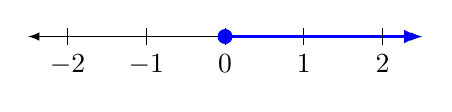
\begin{tikzpicture}
\draw[latex-latex] (-2.5,0) -- (2.5,0) ; %edit here for the axis
\draw [very thick, - latex, blue] (0,0) -- (2.5,0);
\node[circle,draw=blue, fill=blue, inner sep=0pt,minimum size=5pt] (a) at (0,0) {};
\foreach \x in  {-2,-1,0,1,2} % edit here for the vertical lines
\draw[shift={(\x,0)},color=black] (0pt,3pt) -- (0pt,-3pt);
\foreach \x in {-2,-1,0,1,2} % edit here for the numbers
\draw[shift={(\x,0)},color=black] (0pt,0pt) -- (0pt,-3pt) node[below] 
{$\x$};
\end{tikzpicture}
\end{center}

\end{example}

\begin{remark}
While we will only refer to the domain and range of a function, there is another set that you may encounter relating to functions: the \textbf{codomain}. When we use the notation
$$f:A\to B$$
to represent a function, the set $A$ is the domain but the set $B$ is called the \textit{codomain} and does not have to be the same as the range of the function. The range of a function is either equal to or is a subset of the codomain. For example, when looking at the function $f:\mathbb{R}\to\mathbb{R}$ defined by $f(x) = x^2$ in Example \autoref{ex:xsquared}, the codomain is $\mathbb{R}$ while the range is the set of numbers greater than or equal to $0$. 
\end{remark}

\begin{example}[A Function with a Square Root]\label{ex:introsqrt}
Consider the function $g(x) = \sqrt{4-x}$. We can successfully use the value $x=0$ as an input because
$$g(0) = \sqrt{4-0}=\sqrt{4}=2$$
So we see that the output $g(0)=2$ is defined as the input of $x=0$, hence $x=0$ is in the domain of $g$. Similarly, we can plug in the values $x=1, 2, 3,$ and $4$, along with the values $x=-1, -2,-3$ and $-4$:

\begin{table}[H] % Use [H] to suppress floating and place the figure/table exactly where it is specified in the text
	\centering % Horizontally center the table on the page
	\begin{tabular}{c c c c c c c c c c}
		\toprule
		$x$ & $-4$ & $-3$ & $-2$ & $-1$ & 0 & 1 & 2 & 3 &4\\
		\midrule
		$g(x)$ & $\sqrt{8}$ & $\sqrt{7}$ & $\sqrt{6}$ & $\sqrt{5}$ & 2 & $\sqrt{3}$ & $\sqrt{2}$ & $\sqrt{1}=1$ & $\sqrt{0}=0$\\
		\bottomrule
		\end{tabular}
	\caption{A table of values of the function $g(x)=\sqrt{4-x}$.}
	\label{tab:introsqrt} % Unique label used for referencing the table in-text
\end{table}

However, if we try to plug in $x=5$, we do not get an output because we cannot take square roots of negative numbers:
$$g(5) = \sqrt{4-5} = \sqrt{-1}\text{ is undefined}.$$
Thus $x=-4, -3,\ldots, 3, 4$ ARE in the domain of $g$ while $x=5$ is NOT in the domain of $g$. How can we determine exactly where the domain begins and ends? Since we need the quantity inside the square root to be non-negative, meaning 0 or greater, we set up and solve the inequality
$$\begin{aligned}
4-x &\geq 0\\
+x & & +x\\
\hline
4 &\geq x
\end{aligned}$$
Hence any value of $x$ that is equal or less than 4 is in the domain, which we write as either $x\leq 4$ or $(-\infty,4]$. 

Determining the range of $g(x)$ is aided by looking at a graph:


\begin{figure}[] % Use [H] to suppress floating and place the figure/table exactly where it is specified in the text
	\centering % Horizontally center the figure on the page
	\includegraphics[width=0.5\textwidth]{introsqrt.png} % Include the figure image
	\caption{A graph of the function $y=\sqrt{4-x}$.}
	\label{fig:introsqrt} % Unique label used for referencing the figure in-text
\end{figure}

Thus we see that the smallest value we can get as an output is $y=0$, while it looks like the values of $y$ continue to increase as the values of $x$ become more and more negative. Thus from the graph, it appears that the range of the function is $y\geq 0$. 

\end{example}


\begin{example}[A Function with a Denominator]\label{ex:graphfunction}
Below is the graph  of the function $h(x) = \dfrac{1}{x^2-4}$. Note that even though there are three distinct curves that make up the graph, each $x$-value only has one part of the curve above or below it, so we can determine from the curve the associated $y$-value given by the function. For instance, the point on the graph $(1,h(1))$ is plotted in blue, and we can estimate from the picture that $y=h(1)\approx -0.3$. Finding the precise value from the formula, we see that
$$h(1) = \dfrac{1}{1^2-4} = \frac{1}{1-4} = -\frac{1}{3}.$$

\begin{figure}[H] % Use [H] to suppress floating and place the figure/table exactly where it is specified in the text
	\centering % Horizontally center the figure on the page
	\includegraphics[width=0.65\textwidth]{Ch1Sec1RationalFunction.png} % Include the figure image
	\caption{A graph of the function $y=h(x)$.}
	\label{fig:ch1sec1rationalfunction} % Unique label used for referencing the figure in-text
\end{figure}

Looking closely at the graph, it appears that the parts of the curve near $x=-2$ and $x=2$ become nearly vertical, and it's not clear what $y$-value we are meant to use for $h(-2)$ and $h(2)$. In fact, there are NO $y$-values associated with $h(-2)$ and $h(2)$; $x=-2$ and $x=2$ are not in the domain of this function! 

We can see algebraically that when we try to compute the value of the function at $x=-2$, we end up dividing by $0$, which is undefined:
$$h(-2)  = \frac{1}{(-2)^2-4} = \frac{1}{4-4} = \frac{1}{0}\text{, which is undefined.}$$
Similarly, $h(2)$ is undefined:
$$h(2)  = \frac{1}{(2)^2-4} = \frac{1}{4-4} = \frac{1}{0}\text{, which is undefined.}$$
These are the only $x$-values for which the denominator is equal to $0$,\footnote{You will learn how to determine this in  \autoref{sec:linearandquadraticfunctions}.} so we can confirm from both the graph and the formula of the function $h$ that its domain is 
$$x\neq -2,2.$$
which we can write using interval notation as
$$x\in (-\infty,-2)\cup(-2,2)\cup(2,\infty).$$
The round parentheses mean we do not include the endpoints at $-2$ and $2$, and  $\cup$ is the "union" symbol, which means we are glueing the intervals together. 

From the graph, it appears that the range of $y=h(x)$ does not include all values of $y$; the right- and left-most parts of the graph approach the $x$-axis, and so the $y$-values get close to $0$, but the middle part of the graph has a distinct gap at the top and the $y$-values do not seem to quite reach 0. 
Experiment with the graph of $y=h(x)$ by clicking on the Desmos graph 
\begin{quotation}\href{https://www.desmos.com/calculator/7sh4jaq0ox}{https://www.desmos.com/calculator/7sh4jaq0ox}. 
\end{quotation}
The point $(a,h(a))$ is plotted in purple and there is a slider where you can adjust the values of $a$. Note that Desmos gives a value for $y=h(a)$ everywhere except for when $a=-2$ and $a=2$. 

We can see using the Desmos graph that the highest point on the middle part of the graph occurs at $x=0$ when $h(0) = -\frac{1}{4} = -0.25$. Thus the range of $h(x)$ includes all values of $y$ that are greater than 0, from the left and right curves, or that are less than or equal to $-\frac{1}{4}$, from the middle curve. This is written in interval notation as:
$$(-\infty,-1/4)\cup(0,\infty)$$%Can you determine from the graph what the range of the function $h(x)$ is? %\todo{Range of $h(x)$ on worksheet?}


\end{example}




\subsection{Non-Functions and the Vertical Line Test}

So, what {\it isn't} a function? If a rule assigns a real-number input to more than one output, then that rule is not a function. In this subsection, we learn a theorem to help us determine graphically whether or not a relationship is a function. 


\begin{example}[A Non-Example]
For example, consider the relationship between the independent variable $x$ and the dependent variable $y$ where the square of $y$ is equal to $x$. We could write this as $y^2 = x$, where we remember that the input is $x$. For example, if we take $x=4$, then the output $y$ is a number that squares to $4$. This could be either $y=2$ or $y=-2$, since $2^2=4$ and $(-2)^2 = 4$. Since we don't know which to choose, we say that "$y$ is not defined as a function of $x$." 

Algebraically, we could try to "solve" the equation $y^2=x$ for $y$ by writing $y=\pm\sqrt{x}$, and we see that we have the same issue where the input $x=4$ corresponds to \underline{two} different $y$-values, both $y=-2$ and $y=2$. 

If you think of a function as a machine or algorithm that is required to return a single value, this ambiguity in having either $y=2$ or $y=-2$ as our output can be thought of as a program that crashes and fails to complete its task. 
\end{example}

Here is another example of a relationship between variables that does not describe a function. 

\begin{example}[A relationship described by a formula and graph that is NOT a function]
%APC 1.2.4 a
The relationship between the variables $x$ and $y$ given by the equation
$$x^2+y^2=16$$
is graphed in \autoref{fig:ch1sec1circle} below in red. 

\begin{figure}[] % Use [H] to suppress floating and place the figure/table exactly where it is specified in the text
	\centering % Horizontally center the figure on the page
	\includegraphics[width=0.5\textwidth]{Ch1Sec1Circle.png} % Include the figure image
	\caption{The red circle is the points $(x,y)$ that satisfy the equation $x^2+y^2=16$.}
	\label{fig:ch1sec1circle} % Unique label used for referencing the figure in-text
\end{figure}

If we let $x=1$, we can solve for $y$:
$$\begin{aligned}
(1)^2+y^2 &=16\\
y^2 &=16-1\\
y^2 &=15\\
y &= \pm\sqrt{15}\approx \pm3.873
\end{aligned}$$
The points $(1,\sqrt{15})$ and $(1,-\sqrt{15})$ are labeled in blue and green, respectively. Thus we see that when $x=1$, there are \textit{two} $y$-values given by the equation instead of $1$, and without more information, we do not know which to use. So we see that $y$ cannot be defined as a function of $x$ from the equation $x^2+y^2=16$, even though it defines a very nice curve (a circle of radius 4). 

Note that $x=1$ was picked at random. You can see from the picture of the circle that there are many other points where a single $x$-value corresponds to two different $y$-values, in particular anywhere that a vertical line passes through the circle twice. 

\end{example}

Let's summarize the key property that determines whether or not a relationship or process is a function: 
\begin{quotation}
each input has one and only one output. 
\end{quotation}
Thus, the usual way to demonstrate that a relationship or process is \textit{not} a function is to find a particular input that is associated with two or more outputs. When the relationship is given graphically, we can use the vertical line test to determine whether or not the graph represents a function:

\begin{theorem}[The Vertical Line Test]\index{Functions!Vertical Line Test}\label{thm:vlt}
A graph represents a function if and only if every vertical line intersects the graph in at most one point. 

When the graph passes this test, the vertical coordinate of each point on the graph can be viewed as a function of the horizontal coordinate of the point. When the graph does not pass this test, the vertical coordinate cannot be viewed as a function of the horizontal coordinate. 
\end{theorem}




\begin{example}[A graph that is not a function]
In \autoref{fig:TaalmanPage39b}, the marked vertical line passes through the graph twice, and so the graph does not pass the Vertical Line Test. Thus the vertical coordinate $y$ cannot be viewed as a function of the horizontal coordinate $x$. 

\begin{figure}[H] % Use [H] to suppress floating and place the figure/table exactly where it is specified in the text
	\centering % Horizontally center the figure on the page
	\includegraphics[width=0.35\textwidth]{TaalmanPage39b.png} % Include the figure image
	\caption{A graph that does not pass the Vertical Line Test is not a function.}
	\label{fig:TaalmanPage39b} % Unique label used for referencing the figure in-text
\end{figure}

This graph corresponds to the equation $y^2-4y = x-5$. Because we already know from the Vertical Line Test that $y$ is not a function of $x$, we \textit{cannot} rewrite this equation as $y=f(x)$, where $f(x)$ is some expression involving only the variable $x$. 
\end{example}

\begin{exercise}
Think about a relationship between two quantities in an area of your own interest that satisfies the definition of a function. First, give a verbal description of this relationship. Next, pick variable names for each of the quantities involved and specify which is the independent and dependent variable. Lastly, explain why this relationship assigns to each input one and only one output (in other words, the relationship passes the Vertical Line Test if you graph the dependent variable on the vertical axis and the independent variable on the horizontal axis).
\end{exercise}




\begin{example}\label{ex:functionexamples}
Which of the relationships below are functions? Which are not?

    \begin{enumerate}[label=\large{\textbf{\alph*.}},itemsep=20pt,topsep=20pt]
\item The relationship between the circumference of a circle and its diameter. 
\item The relationship between people and phone numbers. 
\item %From APC Activity 1.1.2 and Section 1.1.2
\label{ex:conicaltank1-1} The relationship between $t$ and $V$ given by \autoref{tab:conicaltank1-1}.


\begin{table}[H] % Use [H] to suppress floating and place the figure/table exactly where it is specified in the text
	\centering % Horizontally center the table on the page
	\begin{tabular}{c c c c c c c}
		\toprule
		$t$ & $0$ & $1$ & $2$ & 3 & 4 & 5 \\
		\midrule
		$V$  & 0 & $0.75$ & $1.5$ & $2.25$ & $3.0$ & $3.75$ \\
		\bottomrule
		\end{tabular}
	\caption{A relationship between $t$ and $V$.}
	\label{tab:conicaltank1-1} % Unique label used for referencing the table in-text
\end{table}
\item The relationship between $x$ and $y$ given by \autoref{tab:notfunc}. 

\begin{table}[H] % Use [H] to suppress floating and place the figure/table exactly where it is specified in the text
	\centering % Horizontally center the table on the page
	\begin{tabular}{c c c c c c c c}
		\toprule
		$x$ & $3$ & $2$ & $-1$ & 0 & 1 & 2 & 3\\
		\midrule
		$y$ & $-9$ & $-7$ & $1$ & 0 & 1 & 4 & 9\\
		\bottomrule
		\end{tabular}
	\caption{A relationship between $x$ and $y$.}
	\label{tab:notfunc} % Unique label used for referencing the table in-text
\end{table}


%\item The relationship between $x$ and $f(x)$ given by the rule $f(x) = 2-\sqrt{x+5}$
%
%\item The relationship between $x$ and $y$ given by the graph 
%
%\begin{figure}[H] % Use [H] to suppress floating and place the figure/table exactly where it is specified in the text
%	\centering % Horizontally center the figure on the page
%	\includegraphics[width=0.6\textwidth]{Ch1Sec1RationalFunctiona.png} % Include the figure image
%	\caption{A graph of a relationship between $x$ and $y$.}
%	\label{fig:ch1sec1rationalfunctiona} % Unique label used for referencing the figure in-text
%\end{figure}
%

\end{enumerate}

\end{example}


\begin{solution}
\begin{enumerate}[label=\textbf{\alph*.},itemsep=10pt]
\item The relationship between the circumference of a circle and its diameter is a function. If we are given a diameter, we can determine the circumference of the correspondingly sized circle in an unambiguous way. Can you remember how? This will be answered later in this section. 

\item %APC Example 1.2.12
The relationship between people and phone numbers is NOT a function. \\

A given individual person can be associated with more than one phone number, such as their cell phone and their work telephone. This means that we can't view phone numbers as a function of people: one input (a person) can lead to two different outputs (phone numbers). We also can't view people as a function of phone numbers, since more than one person can be associated with a phone number, such as when a family shares a single phone at home.


\item The relationship between  $t$ and  $V$  is a function. If we view $t$ as the independent variable, there is only one value of $V$ associated to each. The reverse is also true: if we view $V$ as the independent variable, there is only one value of $t$ associated to each. 


\item \autoref{tab:notfunc}  does NOT represent a function. $y$ cannot be a function of $x$ because if $x$ is the independent variable, the input $x=3$ corresponds to two different outputs $y=-9$ and $y=9$. Similarly, the input $x=2$ corresponds to two different outputs $y=-7$ and $y=4$. \\

We also cannot view $x$ as a function of $y$ because if $y$ is the independent variable, the input $y=1$ corresponds to two different outputs $x=-1$ and $x=1$.  


%\item The relationship between $x$ and $f(x)$ given by the rule $f(x) = 2-\sqrt{x+5}$ defines a function.  
%
%\item The relationship between $x$ and $y$ given by the graph in \autoref{fig:ch1sec1rationalfunctiona} defines $y$ as a function of $x$. Even though there are three distinct curves that make up the graph, each $x$-value only has one part of the curve above or below it, so we can determine from the curve the associated $y$-value given by the function. \\
%
%However, the graph in \autoref{fig:ch1sec1rationalfunction} does NOT define $x$ as a function of $y$ since, for example, $y=5$ corresponds to two different $x$-values (it looks from the picture like $x\approx -2$ and $x\approx 2$). 
\end{enumerate}
\end{solution}

%Now let's take a closer look at some of the functions described in Example \autoref{ex:functionexamples} in order to practice our new terminology of independent and dependent variables, domain, and range. 


\subsection{Real-world Examples of Functions}

Let's take a closer look at two of the functions described in Example \autoref{ex:functionexamples} in order to get a sense of how functions can be used in the real-world.

\begin{example}[A function described in words]
%https://mathshistory.st-andrews.ac.uk/HistTopics/Pi_through_the_ages/
%https://www.exploratorium.edu/pi/history-of-pi#:~:text=1650%20BC)%20gives%20us%20insight,mathematicians%20of%20the%20ancient%20world
Consider again the function defined by the relationship between the circumference of a circle and its diameter. The circumference of a circle is \textbf{directly proportional} to the diameter of the circle, meaning that the ratio of the two quantities is a constant value. The ratio of the circumference to the diameter of a circle\footnote{Chinese mathematician and astronomer Zu Chongzhi (429–501) estimated the value of $\pi$ by calculating the value of the ratio of the circumference of a circle to its diameter. His approximation was $355/113$. Other historical mathematicians independently estimated $\pi$ using the ratio of the area and radius of a circle. The ancient Babylonians (ca. 1900–1680 BC) estimated $\pi$ as $3.125$. On the Rhind Papyrus (ca.1650 BC), Egyptian mathematicians recorded the value of $\pi$ as 3.1605. Archimedes of Syracuse (287–212 BC) showed that $\pi$ is between $3\frac{1}{7}$ and $3\frac{10}{71}$. \href{https://www.exploratorium.edu/pi/history-of-pi}{https://www.exploratorium.edu/pi/history-of-pi} accessed August 4, 2022.} happens to be the constant value $\pi$, so we can write this relationship explicitly as
$$\frac{C}{d}=\pi$$
where $C$ represents the circumference and $d$ is the diameter. If we choose to make $C$ the \textit{dependent variable}  and $d$ the \textit{independent variable}, we can rewrite this relationship so that $C$ is a function of $d$:
$$C=\pi d.$$
Given the diameter of a circle, you can find its circumference by multiplying by $\pi$. 
%Could we also rewrite this relationship so that $d$ is a function of $C$? Think about it\ldots
\end{example}


%\todo{worksheet problem: area as a function of radius, relationship between radius and diameter, is the relationship between the area and circumference of a circle a function? If it is, find a formula for one in terms of the other}


\begin{example}[A function described in a table]\label{ex:tablefunction}
Recall the table of values in \autoref{tab:conicaltank1-1}. Typically, we would view $t$ as the \textit{independent variable} and view $V$ as the \textit{dependent variable}, meaning that $V$ is a function of $t$, which we could write as $V=f(t)$. If we read from the table alone without any interpretation, the domain for the function $V=f(t)$ is $\text{Domain}(V) = \in\{0, 1, 2, 3, 4,5\}$ while the range is $\text{Range}(V) = \{0, 0.75, 1.5, 2.25, 3.0, 3.75\}$. 


Now we add some context! Consider a tank in the shape of an inverted circular cone (point down) where the tank's radius is 2 feet and its depth is 4 feet. See \autoref{fig:conicaltank1-1} below. 

\begin{figure}[H]
	\centering
	\begin{subfigure}[H]{0.4\textwidth}
    		\centering
    		\includegraphics[width=0.7\textwidth]{APCFigure1-1-7.png}
    		\caption{The empty conical tank.}
    		\label{fig:conicaltank1-1a}
	\end{subfigure}
	\hspace{.5in}
	\begin{subfigure}[H]{0.4\textwidth}
		\centering
		\includegraphics[width=0.7\textwidth]{APCFigure1-1-8.png}
		\caption{The conical tank, partially filled.}
		\label{fig:conicaltank1-1b}
	\end{subfigure}
\caption{A tank in the shape of an inverted circular cone (point down) with radius 2 feet and depth 4 feet is being filled with water.}
\label{fig:conicaltank1-1}
\end{figure}

Suppose that the tank is being filled with water that is entering at a constant rate of $0.75$ cubic feet per minute. Initially, there is no water in the tank and after each subsequent minute, there is $0.75$ ft$^3$ more water in the tank. \autoref{tab:conicaltank1-1b} below summarizes the relationship between the time $t$ that has passed and the volume $V$ of the water in the tank. This is the same as \autoref{tab:conicaltank1-1}, except that now $t$ represents time and $V$ represents volume in a physical context where water is being added continuously to the tank. 


\begin{table}[H] % Use [H] to suppress floating and place the figure/table exactly where it is specified in the text
	\centering % Horizontally center the table on the page
	\begin{tabular}{c c c c c c c}
		\toprule
		$t$ (in minutes) & $0$ & $1$ & $2$ & 3 & 4 & 5 \\
		\midrule
		$V$ (in ft$^3$) & 0 & $0.75$ & $1.5$ & $2.25$ & $3.0$ & $3.75$ \\
		\bottomrule
		\end{tabular}
	\caption{How time and volume change in tandem in a conical tank.}
	\label{tab:conicaltank1-1b} % Unique label used for referencing the table in-text
\end{table}


We can now use some of our intuition from this new context to interpret the table. In the first five minutes, the values for $V$ tell us that the tank starts at 0 ft$^3$ of water (empty) and fills to $3.75$ ft$^3$ of water. We know that the volume is increasing steadily and so contains \textit{all values} between 0 and $3.75$, and no values outside that range, during the time frame from $t=0$ to $t=5$.  These are significant assumptions that come from our knowledge of the physical setting of the problem! Based on this deeper interpretation, we can say that on a domain of $t$ between 0 and 5 minutes, the range for $V$ is from 0 to $3.75$ ft$^3$. 

Exercise \autoref{ex:conicaltank1-1exercise} will have you explore this function in even greater depth (no pun intended). We will also review it during class, but if you have time you should attempt it now. 



%But what if we allow the tank to keep filling until it overflows? In general, the volume of a cone is 
%$$V=\frac{1}{3}\pi r^2h$$
%and so the volume of the entire cone is $\frac{1}{3}\pi (2)^2(4) = \frac{48\pi}{3}\approx 50.2655$ ft$^3$. Thus the range for the function until the cone overflows is from 0 to approximately $50.2655$ ft$^3$, representing the amount of water in the cone up from when it is empty to when it is full. One way to write this mathematically is using inequalities: 
%$$0\leq V\leq 50.2655$$
%which is read "0 is less than or equal to $V$, which is less than or equal to $50.2655$".
%
%Another way is using interval notation:
%$$V\in[0,50.2655]$$
%which is read "$V$ is in the set of numbers from 0 (inclusive) to $50.2655$ (inclusive)." The symbol $\in$ means "in" and the square brackets indicate the the endpoints of the interval are included. 
\end{example}







%
%\begin{example}[A function described by a formula]\label{ex:formulafunction}
%$f(x) = 2-\sqrt{x+5}$ is a formula that describes a function. For each value $x$ for which the formula makes sense, there is exactly one real number described by $2-\sqrt{x+5}$.  However, we have to be careful what values we allow for $x$, meaning what numbers are in the \textit{domain} of the function. Recall that you cannot take the square root of a negative number. For instance, $x=-10$ will result in $f(-10) = 2-\sqrt{-10+5} = 2-\sqrt{-5}$, which is undefined; if you plug it into a calculator, you will get an error message! What are the values of $x$ that are in the domain? Plug in a few different values for $x$ and see when the quantity $x+5$ under the square root is negative. 
%
% After a bit of guess and check,\footnote{You will learn how to solve this algebraically in Section \ref{sec:solvinginequalities}.} we can see that any value of $x$ that is smaller than $-5$ will make the $x+5$ in the square root negative and the function undefined. Thus we are allowed to use values of $x$ that are $-5$ or greater, so the domain of the function is 
%$$x\geq -5, $$
%read "$x$ is greater than or equal to  negative 5". %or if we want to use interval notation, it is
%%$$x\in[5,\infty),$$
%%read "$x$ is in the interval from 5 (inclusive) to infinity," where by "infinity" we mean that the values become  larger and larger without any upper limit to what they can be.
%
%We can confirm the domain by graphing the function on Desmos:
%
%\begin{figure}[H] % Use [H] to suppress floating and place the figure/table exactly where it is specified in the text
%	\centering % Horizontally center the figure on the page
%	\includegraphics[width=0.65\textwidth]{Ch1Sec1SquareRootFunction.png} % Include the figure image
%	\caption{A graph of the function $f(x)=2-\sqrt{x+5}$.}
%	\label{fig:ch1sec1squarerootfunction} % Unique label used for referencing the figure in-text
%\end{figure}
%
%It looks from the graph that the range of the function may be $y\leq 2$, but we can't be certain. %Explore the graph and see whether you think that is the range, or if it is something else: \href{https://www.desmos.com/calculator/mnekavlqzl}{https://www.desmos.com/calculator/mnekavlqzl}. 
%
%
%\end{example}
%


%
%\begin{exercise}
%\autoref{fig:ch1sec1squarerootfunction} was generated using Desmos, an online graphing calculator. Click on this link \href{https://www.desmos.com/calculator/tst09nwwvz}{https://www.desmos.com/calculator/tst09nwwvz} to open a window with the graph on your computer. 
%
%Near the top on the left, you will see a slider for the letter $a$. Drag the slider left and right to change the value of $a$. On the graph, you will see a green dot corresponding to the point $(a,f(a))$ on the graph that moves as you change the value of $a$. 
%
%\begin{enumerate}[label=\alph*.]
%\item The values of $a$ are currently set to stay between $-5$ and $10$, making that the \textit{domain} for the points that you can move around with the slider. What is the corresponding \textit{range} for that choice of domain, meaning what are the outputs of the function that you can get if the inputs are between $-5$ and $10$? You might need to zoom out on the graph to be able to see. 
%
%\item You can change the domain of the slider for $a$ by clicking on the $-5$ and $10$. Define at least one other domain for $a$ and give the corresponding range for that domain. For example, you could write:
%\begin{quotation}
%"For input values of $a$ between $\_\_\_$ and $\_\_\_$, the output values $y=f(a)$ are between $\_\_\_$ and $\_\_\_$."
%\end{quotation}
%
%\item The domain of the entire function $f(x) = 2-\sqrt{x+5}$ is the set $x\geq -5$. Confirm that by seeing that values of $a$ smaller than $-5$ do not generate a point on the graph. Convince yourself that the entire range of $f(x) =2-\sqrt{x+5}$ is $y\leq 2$ by zooming out on the graph far enough to see that the values of $y$ continue to decrease without any limit. How large does $x$ need to be in order to have, say, $y=-10$? $y=-100$? 
%\end{enumerate}
%\end{exercise}
%
%




\begin{exercise}\label{ex:conicaltank1-1exercise}
Recall the conical tank being filled with water in Example \autoref{ex:tablefunction}. The table of values that we are given stops at $t=5$ seconds. How long could we continue to fill the tank before it overflows?

\begin{enumerate}[label=\alph*.]
\item Plot the points given in \autoref{tab:conicaltank1-1b} on a set of axes with time $t$ in minutes on the horizontal axis and volume $V$ in ft$^3$ on the vertical axis. What shape does the graph of the function seem to be?
\item Try to think of a formula for the function that gives the volume as a function of time, meaning a formula for $V=f(t)$. Use your graph from part (a) as inspiration.
\item Graph your formula from part (b) for $V=f(t)$ (using Desmos) and confirm our earlier intuition that if $t$ takes on all values between $0$ and $5$, $V$ steadily increases from $0$ to $3.75$, and takes on no values outside of that range. 
\item Now return to your intuitive understanding of the problem. What is the total volume of the conical tank?\footnote{Hint: the volume of a cone is $V=\frac{1}{3}\pi r^2h$.} What does this tell you about the largest possible volume of water in the cone? Use this and your formula for $V=f(t)$ to determine how long it will take for the cone to overflow. 

%\textit{Challenge:} Think about how the height of the water changes in tandem with time. Without attempting to determine specific values of $h$ at particular values of $t$, how would you expect the data for the relationship between $h$ and $t$ to appear? Sketch at least one possible graph on a set of axes with time $t$ in minutes on the horizontal axis and height $h$ in feet on the vertical axis. 
\end{enumerate}
\begin{figure}[H]
	\centering
	\includegraphics[width=0.4\textwidth]{APCFigure1-1-8.png}
	\caption{The conical tank, partially filled.}
	\label{fig:conicaltank1-1d}
\end{figure}
\end{exercise}

%\todo{More on the cone/water rising on the worksheet. Shape of the graph of h as a function of t. Range for h. If having students do algebra relating circumference and area, could do volume and height; nice teaser for similar triangles. Check APC for more follow-up questions. }





\subsection{Interval Notation for Sets}

When we talk about functions, they will always take some set of numbers as their domain and have some set of numbers as their range. In this section, we talk briefly about what a "set" is and some different notations for how to write them down. 

You have already seen one mathematical shorthand for a commonly used set: $\mathbb{R}$ denotes the set of all real numbers. Another useful notation is the \textbf{empty set}: $\emptyset$ denotes the set that contains nothing. 

\begin{remark}
Please do not confuse $\emptyset$ with the number 0. They are VERY different and should NOT be used interchangeably. 
\end{remark}

Another set we discussed was the domain and range of the water in the tank in Example \autoref{ex:tablefunction}. We said that if the time $t$ is between 0 and 5 minutes, then the volume $V$ was between 0 and $3.75$ ft$^3$. We can write these using inequalities:
$$0\leq t\leq 5 \qquad\text{and}\qquad 0\leq V \leq 3.75,$$
which are read "0 is less than or equal to $t$, which is less than or equal to 5" and "0 is less than or equal to $V$, which is less than or equal to $3.75$." An alternate notation for writing these two sets is called \textbf{interval notation}. The set $0\leq t \leq 5$ is written 
$$[0,5]$$
and the set $0\leq V\leq 3.75$ is written
$$[0,3.75].$$
This notation is nice and concise, but does not specify a variable and so can be confusing or ambiguous. If we wish to name the variable $t$, we would write $t\in[0,5]$, read "$t$ is in the set of numbers from 0 (inclusive) to 5 (inclusive)." Likewise for $V$, we can write $V\in[0,3.75]$, read "$V$ is in the set of numbers from 0 (inclusive) to 3.75 (inclusive)." The symbol $\in$ means "in" and the square brackets indicate the the endpoints of the interval are included.

%If we did not want to include the endpoints of the intervals, we would leave out the bar under the inequality and use parentheses instead of square brackets: $0<t<5$ is read "$0$ is less than $t$, which is less than 5" and means that $t$ is strictly between 0 and 5. The corresponding interval notation is $(0,5)$ or $t\in (0,5)$, which is read "$t$ is in the set of numbers between 0 and 5, not inclusive." Likewise, $0<V<3.75$ is read "0 is less than $V$, which is less than $3.75$" and can be written in interval notation as $(0,3.75)$ or $V\in(0,3.75)$, read "$V$ is in the set of numbers from 0 to $3.75$, not inclusive." 

Other sets that you saw were the domain and range of the function $g(x) = \sqrt{4-x}$ in Example \ref{ex:introsqrt}. The range $y\geq 0$ can be written in interval notation as $y\in [0,\infty)$. The domain $x\leq 4$ can be written in interval notation as $x\in (-\infty,4]$. The meaning of this set is best illustrated on a number line:

\begin{center}
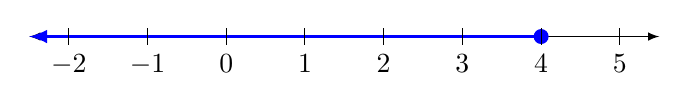
\begin{tikzpicture}
\draw[latex-latex] (-2.5,0) -- (5.5,0) ; %edit here for the axis
\draw [very thick,  latex-, blue] (-2.5,0) -- (4,0);
\node[circle,draw=blue, fill=blue, inner sep=0pt,minimum size=5pt] (a) at (4,0) {};
\foreach \x in  {-2,-1,0,1,2, 3, 4,5} % edit here for the vertical lines
\draw[shift={(\x,0)},color=black] (0pt,3pt) -- (0pt,-3pt);
\foreach \x in {-2,-1,0,1,2, 3, 4,5} % edit here for the numbers
\draw[shift={(\x,0)},color=black] (0pt,0pt) -- (0pt,-3pt) node[below] 
{$\x$};
\end{tikzpicture}
\end{center}

The values of $x$ are allowed to be any number below $x=4$, denoted by the open parentheses and $-\infty$ on the left of the interval $(-\infty,4]$. 


Another set that you saw was the domain of the function $h$ in Example \autoref{ex:graphfunction}. We wrote this using the standard shorthand of $x\neq -2,2$, which means that $x$ can take on any value except for $-2$ and $2$. To write this using inequalities, we would need three different parts:
$$x<-2\quad\text{or}\quad -2<x<2\quad\text{or}\quad 2<x.$$
The corresponding interval notation also has three parts:
$$(-\infty,-2)\cup(-2,2)\cup(2,\infty). $$
The round parentheses mean we do not include the endpoints at $-2$ and $2$, and  $\cup$ is the "union" symbol, which means we are glueing the intervals together. 

Finally, one more standard notation is an alternate way of writing the set of all real numbers: instead of writing $\mathbb{R}$, we can write $(-\infty,\infty)$. There is no way to write the empty set $\emptyset$ using interval notation; WeBWorK will typically have you enter the word "none" in cases where there is no solution.

Here is a table summarizing all of the above examples, along with a few more to help you understand when to use "$($" vs. "$[$" and how to incorporate "$\cup$".

\begin{table}[H] % Use [H] to suppress floating and place the figure/table exactly where it is specified in the text
	\centering % Horizontally center the table on the page
	\begin{tabular}{c c}
		\toprule
		& \textbf{Interval notation}\\
		\midrule
		$\mathbb{R}$ & $(-\infty,\infty)$\\
		\midrule
		$\emptyset$ & none\\
		\midrule
		$0\leq t\leq 5$ & $[0,5]$ or $t\in [0,5]$\\
%		\midrule
%		$0<t<5$ & $(0,5)$ or $t\in(0,5)$\\
		\midrule
		$0\leq V\leq 3.75$ & $[0,3.75]$ or $V\in [0,3.75]$\\
%		\midrule
%		$0<V<3.75$ & $(0,3.75)$ or $V\in(0,3.75)$\\
		\midrule
		$x\leq 4$ & $(-\infty, 4]$ or $x\in (-\infty,4]$\\
		\midrule
		$y\geq 0 $ & $[0,\infty)$ or $y\in[0,\infty)$\\
		\midrule
		$x\neq -2,2$ & $(-\infty,-2)\cup(-2,2)\cup(2,\infty)$\\
		\midrule
		$-1\leq x<3$ & $[-1,3)$\\
		\midrule
		$-1<x\leq 3$ & $(-1,3]$\\
		\midrule
		$x<-4$ or $x\geq 5$ & $(-\infty,-4)\cup [5,\infty)$\\
		\midrule
		$-3\leq x\leq 7$ and $x\neq 0$ & $[-3,0)\cup(0,7]$\\
		\bottomrule
		\end{tabular}
	\caption{A table of intervals written using interval notation.}
	\label{tab:intervalnotation} % Unique label used for referencing the table in-text
\end{table}


%\subsection{Properties of Functions}
%
%\todo{I think this is going to have to wait for the next section. I feel like this section is long enough.}


\subsection*{Summary}
The following terms were introduced in this section: 
\begin{quotation}
function, set $\mathbb{R}$ of all real numbers, domain, range, function notation, independent variable, dependent variable, graph,  directly proportional, interval notation, the empty set $\emptyset$
\end{quotation}

\textbf{Key ideas:} A relationship or process is a function if each individual input is associated with one and only one output. This is represented visually on graphs via the Vertical Line Test. There are four different ways to represent a function (words, formula, table, graph). The domain of a function is the set of all inputs with a defined output. The range of a function is the set of all realized outputs. 

\textbf{Other ideas introduced:}\footnote{You do not have to understand them now and likely have many questions about them. We will work on these ideas much more over the next few sections. } interval notation will become a convenient way to represent sets of numbers, the inside of a square root cannot be negative and the denominator of a fraction cannot be zero, the range of a function is not easy to find without a graph or table.


\begin{center}
\textcolor{ocre}{\fbox{\fbox{\Large \bf \sc End of Section 1.1}}}
\end{center}

\hspace{-.5in}\rule{1.1\textwidth}{2pt}

%----------------------------------------------------------------------------------------
%	Section 2
%----------------------------------------------------------------------------------------



\section{Linear and Quadratic Functions}\index{Functions!Linear Functions}\index{Functions!Quadratic Functions}\label{sec:linearandquadraticfunctions}


\subsection*{Learning Goals}
\begin{itemize}
	\item Understand the definition of linear and quadratic functions. 
	\item Explore how the parameters of a linear or quadratic function change the shape of its graph and its properties. 
	\item Use the different forms for equations for lines. 
	\item Solve quadratic equations via factoring or the quadratic formula. 
\end{itemize}


\subsection{Definitions of linear and quadratic functions}



Linear and quadratic functions are important for modeling relationships between many different quantities. For example, in statistics, the method of Linear Regression seeks to find a line that best describes the relationship between quantities that appear to change at a constant rate relative to each other. Quadratic functions are used to model the height of an object falling under the force of gravity. We will explore several models that use linear and quadratic functions in \autoref{sec:linearandquadraticmodeling} after we develop our mathematical understanding of them. 

We begin with the mathematical definitions of linear and quadratic functions. Recall that a \textit{mathematical definition} is "used to give a precise meaning to a new term, by describing a condition which unambiguously qualifies what a mathematical term is and is not."\footnote{\href{https://en.wikipedia.org/wiki/Definition}{https://en.wikipedia.org/wiki/Definition} accessed August 4, 2022.} Thus the definitions below give us the precise meaning of a linear or quadratic function. Remember that we generally need a few examples to make sense of definitions, and these follow below each of the definitions. 

%From Taalman Section 0.5
%Since linear functions will be central to our study of derivatives, we will spend some time studying them in depth right away. As we will do for all of our investigations of functions in this book, we begin with the algebraic definition:

\begin{definition}[Linear Functions]\label{def:linearfunction}
A {\bf linear function} is a function that can be written in the form $f(x) = mx+b$ for some real numbers $m$ and $b$. Alternately, a linear function can be written as a \textbf{linear equation} $y=mx+b$, where $y$ is a dependent variable of the independent variable $x$. 
\end{definition}



\begin{example}[Examples of linear functions]\label{ex:linfuncs}
Below are three examples of linear functions. 
\begin{enumerate}[label=\textbf{\alph*.}]
\item The equation
$$y=3x+1$$
defines $y$ as a linear function of $x$, taking $m=3$ and $b=1$ in Definition \autoref{def:linearfunction}

\item The equation
$$y=x$$
also defines $y$ as a linear function of $x$ if we rewrite it as
$$y=1\cdot x+0$$
so that we see that we must take $m=1$ and $b=0$. This function, $f(x) = x$ is a special function, called the \textbf{identity function}, where the output and input are the same. 

\item The equation
$$y=1.2$$
is also a linear equation, so defines $y$ as a linear function (the independent variable isn't specified, though we can infer it to be $x$). To see this, rewrite it as
$$y=0\cdot x+1.2$$
so that we can see that we must take $m=0$ and $b=1.2$. $f(x)=1.2$ is an example of a \textbf{constant function}, which is a function of the form $f(x) = b$. For any input, the output is always $b$, meaning the output is a constant number. 
\end{enumerate}
\end{example}

An important detail of the above definition is that a linear function \textit{can} be rewritten in the form $f(x)=mx+b$; it may not look like that originally. 

\begin{exercise}
Rewrite 
$$y=\frac{3x+1}{2}, \quad \text{and} \quad 2y-1=6x$$
in the form $y=mx+b$ and identify $m$ and $b$. These are two more examples of linear functions. 
\end{exercise}




\begin{definition}[Quadratic Function]
A {\bf quadratic function} is one that may be written in the form
$$f(x)=ax^2+bx+c,$$
where $a, b, $ and $c$ are real numbers with $a\neq 0$. Alternately, a quadratic function can be written as a \textbf{quadratic equation} 
$$y=ax^2+bx+c,$$
where $y$ is a dependent variable of the independent variable $x$. 
\end{definition}

Similar to linear functions, quadratic functions \textit{can} be written in the form $f(x) = ax^2+bx+c$ but do not need to begin that way. 

\begin{exercise}
Rewrite each of the expressions below in the form 
$$y=ax^2+bx+c$$
and identify $a, b$, and $c$. These are examples of quadratic functions. 

\begin{enumerate}[label=\roman*.]
\item $y=(x-2)^2$
\item $y=x^3-x(x^2+3x-7)+2$
\item $y=x^2$
%\item $y=a(x-h)^2+k$ \textit{Hint:} In this expression, $a=a$. $b$ and $c$ will be in terms of the letters $h$ and $k$. 
\end{enumerate}
\end{exercise}

%\todo{For worksheet or homework: Is it possible to find a formula for a quadratic function that passes through the points $(0,8)$, $(1,12)$, and $(2,12)$? If yes, do so; if not, explain why not. yes: the quadratic $q(x) = -2x^2+6x+8$ passes through all three points. }


\subsubsection{Parameters}

%From Juliana's F22 MATH1100 handout for parameters

It is important to note that when we write an expression like $f(x) = mx+b$ or $f(x) = ax^2+bx+c$, only $x$ and $y$ are variables. The extra letters $a, b, c,$ and $m$ that are not variables are called \textbf{parameters} of the function. How should you think about these parameters and what they represent? 

While the word \textit{parameter} may be new to you, the concept is probably not so unfamiliar. We can think of a \textit{parameter} as a "dial" on the function machine. Setting the dials to different values creates different functions.\footnote{Analogy and Image from \href{https://mathinsight.org/function\_machine\_parameters}{https://mathinsight.org/function\_machine\_parameters}}



\begin{figure}[H]
	\begin{subfigure}[H]{0.45\textwidth}
    		\centering
    		\includegraphics[width=0.9\textwidth]{mathinsight-functionmachine.png}
    		\caption{Think of a function as a machine that turns inputs into outputs.}
    		\label{fig:func-machine}
	\end{subfigure}
	\hfill
	\begin{subfigure}[H]{0.45\textwidth}
		\centering
		\includegraphics[width=0.9\textwidth]{mathinsight-functionmachine-withdials.png}
		\caption{Parameters are "dials" that adjust how the function machine works.}
		\label{fig:functionmachinewithdials}
	\end{subfigure}
\caption{}
\label{fig:functionmachine}
\end{figure}



\begin{example}[Parameters of Linear Functions] Consider the linear function:

$$y = mx + b.$$

Here $x$ is the independent variable and $y$ is the dependent variable. The letters $m$ and $b$ are parameters of the linear equation. 


    \begin{itemize}
    \item 
    If we choose a specific value of $m$ and $b$ ("set the dials"), we get a specific line. 
    %To get a specific line, we have to choose a specific value of $m$ and $b$ (``set the dials"). 
    
    For example, if $m = 3$ and $b = -7$ we get the linear function $y = 3x - 7$.
    
    \item When we change the dials, we get a different line. %Any given line has a fixed $m$ and $b$. We can change $m$ and $b$ to describe different lines.
    
    \end{itemize}

\end{example}


When we have a \textbf{function with parameters}, we can think of this function representing a whole family of functions, one for each combination of parameter values. 

\begin{exercise}
To get a hands-on feel for this, go to the Desmos site 
\begin{quotation}\href{https://www.desmos.com/calculator/uo5qirntxg}{https://www.desmos.com/calculator/uo5qirntxg}. 
\end{quotation}
You'll see the equation $y = mx+b$ in the top left and below that, sliders for $m$ and $b$ (these are our \textit{parameters}). The graph is currently set for $m = 3$ and $b = -7$. 

\begin{enumerate}[label=\alph*.]
\item Play around with the values of $m$ and $b$. What happens to the graph? What does each parameter represent in this example?
\item Can you find values of $m, b$ that represents a horizontal line? Can you find values of $m, b$ that represents a vertical line? If so, what are they? If not, why not?
\end{enumerate}
\end{exercise}


\begin{example}[Parameters of Quadratic Functions]
Consider the quadratic equation $$y = ax^2 + bx + c,$$ where $a \neq 0$. Graphically, this describes a family of parabolas. 

\autoref{fig:quadfuncfamily} shows a graph of some members of this family. This graph shows parabolas with $a = -2; b = 0, 1, \text{or } 2$; and $c = 2.5$ 
and parabolas with $a = -1; b = 0, 1, \text{or } 2$; and $c = -1$ 



\begin{figure}[H] % Use [H] to suppress floating and place the figure/table exactly where it is specified in the text
	\centering % Horizontally center the figure on the page
	\includegraphics[width=0.7\textwidth]{1100-QuadraticSpecific.png} % Include the figure image
	\caption{$y=ax^2+bx+c$ for different values of the parameters $a, b,$ and $c$.}
	\label{fig:quadfuncfamily} % Unique label used for referencing the figure in-text
\end{figure}
%https://www.desmos.com/calculator/wsazn7prei

\end{example}


\begin{exercise}\label{ex:quadraticparameters}
Take a moment to use \href{https://www.desmos.com/calculator/yayrd6etuz}{https://www.desmos.com/calculator/yayrd6etuz} to explore how changing the values of the parameters $a, b$, and $c$ impact the graph of $y=ax^2+bx+c$. What do the members of the family of parametric functions $y=ax^2+bx+c$ have in common? How do they differ? Which parameter seems to have the simplest effect? Which parameter seems to have the most complicated effect?
\end{exercise}



\subsection{Properties of Functions}\label{subsec:propgraphs1}


%From Taalman Section 0.4
The table that follows gives us vocabulary and precise mathematical definitions for various types of graphical behavior. Rows 1, 2, 5, 6, and 8 describe behaviors that a function could exhibit at a specific point. Rows 3, 4, and 7 describe graphical behaviors that occur over an interval $I$ of real numbers.  


%\todo{Use different letters for the constants here since we are using a, b, c, and m as parameters for linear and quadratic functions. Not sure what to use...}

\begin{remark}
\autoref{tab:funcprops1} uses $x$ as the independent variable and $y$ as the dependent variable. The notation $x_1, x_2, y_1,\ldots$ is used to indicate particular values of $x$ and $y$. We are using these instead of other letters because we have been using other letters to indicate parameters. A subscript is called an "index" (plural "indices"). The benefit to using these is that it is easier to keep track of whether they represent a value of the independent variable (for example, $x=x_1$ or $x=x_2$) or the dependent variable (for example, $y=y_1$ or $y=y_2$). 
\end{remark}


\setlength{\tabcolsep}{14pt}
\begin{table}[H]
\centering
\begin{tabular}{p{0.1in} p{1.25in} p{1.25in} p{1.75in}}
\toprule
&\textbf{Vocabulary} & \textbf{Definition} & \textbf{Behavior}\\
\midrule
1. & $f$ has a \textbf{$x$-intercept} or  {\bf zero}  at $x=x_1$ & $f(x_1)=0$ & graph intersects the $x$-axis at $x=x_1$ \\
\hline
2.  & $f$ has a \textbf{$y$-intercept} at $y=y_1$ & $f(0)=y_1$ & graph intersects the $y$-axis at $y=y_1$ \\
\hline
3. & $f$ is {\bf positive} on $I$ & $f(x)>0$ for all $x\in I$ & graph is above the $x$-axis on $I$ \\
\hline
4. & $f$ is {\bf increasing} on $I$ & $f(x_2)>f(x_1)$ for all $x_2>x_1$ in $I$  & graph moves up as we look from left to right on $I$  \\
\midrule
5. & $f$ has a {\bf local maximum} at $x=x_1$ & $f(x_1)\geq f(x)$ for all $x$ near $x=x_1$  & graph has a relative "hilltop" at $x=x_1$  \\
\hline
6. & $f$ has a {\bf global maximum} at $x=x_1$ & $f(x_1)\geq f(x)$ for all $x\in\text{Domain}(f)$  & graph is the highest at $x=x_1$  \\
\hline
7. & $f$ is {\bf concave up} on $I$ & values of $f$ grow at a faster and faster rate as $x$ increases on $I$  &  graph curves upwards on $I$ like part of a "U" \\
\hline
8. & $f$ has an {\bf inflection point} at $x=x_1$ & $x=x_1\in\text{Domain}(f)$ and the concavity of $f$ changes at $x=x_1$  & graph of $f$ changes from curving upward to curving downward, or vice versa, at $x=x_1$  \\
\bottomrule
\end{tabular}
\caption{Properties of functions in terms of the behavior of their graphs.}
\label{tab:funcprops1} 
\label{tab:funcprops2}% Unique label used for referencing the table in-text
%\addcontentsline{toc}{table}{Table \ref{tab:example}} % Uncomment to add the table to the table of contents
\end{table}


There are similar definitions for negative, decreasing, and concave down behavior, as well as local and global minima. 

Notice that we describe \textbf{extrema} (maxima and minima) by \textit{where} on the $x$-axis they occur, since we can always find the corresponding $y$-values from these $x$-values. The concept of "near" in the description of a local maximum will be made more precise in Chapters 2 and 3. Inflection points and concavity cannot be precisely defined until we learn about \textit{derivatives} in Chapter 3. In that chapter we will also learn ways for algebraically calculating the locations of extrema and inflection points. For now we present them just to set terminology and to familiarize ourselves with various types of function behavior; we will have to be content with examining such things graphically. 


\begin{example}
The $x$-intercepts of $f(x) = 1-3x$ are where $f(x) = 0$, so at the values of $x$ with $1-3x=0$. Solving for $x$:
$$\begin{aligned}
1-3x &= 0\\
1 &=3x\\
\frac{1}{3} &=x
\end{aligned}$$
So we see that $f(x) = 1-3x$ has an $x$-intercept at $x=\frac{1}{3}$. 

View a graph of $f(x)$ via \href{https://www.desmos.com/calculator/uo5qirntxg}{https://www.desmos.com/calculator/uo5qirntxg} and set the sliders to $m=-3, b=1$. From this we see that $f(x)$ is positive (above the $x$-axis) for $x<\frac{1}{3}$ and negative (below the $x$-axis) for $x>\frac{1}{3}$. The graph also tells us that $f(x)$ is decreasing for $x\in\mathbb{R}$, meaning for all values of $x$. 

The graph of $f(x)$ has no local or global maxima or minima. This is true of all linear functions: none of them have any local or global extrema. Similarly, since the graphs of linear functions are lines, they are neither concave up nor concave down and do not have any inflection points. 
\end{example}


\begin{example}
The list that follows at the right describes each of the properties in the table above of the graph $y=f(x)$ shown on the left. 

\begin{center}
\fbox{
\parbox{.9\textwidth}{Use this example to check your understanding of each of the properties, going back and forth between \autoref{tab:funcprops1} and \autoref{fig:TaalmanPage40} to identify each feature.}}
\end{center}



\begin{figure}[H]
	\begin{subfigure}[H]{0.45\textwidth}
    		\centering
    		\includegraphics[width=0.9\textwidth]{TaalmanPage40.png}
%    		\caption{}
%    		\label{}
	\end{subfigure}
	\hfill
	\begin{minipage}{0.6\textwidth}
	\begin{itemize}
	%\begin{subtable}[H]{0.45\textwidth}
		%\centering
			%\begin{tabular}{l}
			\item $x$-intercepts at $x=-3, x\approx -0.4,$ and $x=3$\\
			\item $y$-intercept at $y=-1$\\
			\item local maxima at $x=-2$ and $x=3$\\
			\item global maximum at $x=-2$\\
			\item inflection points at $x=-1$ and $x=2$\\
			\item positive on $(-3,-0.4)$, meaning from $x=-3$ to $x=-0.4$ (non-inclusive)\\
			\item increasing on $(-\infty,-2)$ and $(1,3)$, meaning for $x<-2$ and $1<x<3$\\
			\item concave up on $(-1,2)$
			%\end{tabular}
%		\caption{}
%		\label{}
	%\end{subtable}
	\end{itemize}
	\end{minipage}
\caption{The graph of $y=f(x)$ (left) and its properties (right).}
\label{fig:TaalmanPage40}
\end{figure}


\end{example}

%A linear function $f(x) = mx+b$ has exactly one root if $m\neq 0$, and either no roots or infinitely many roots if $m=0$. To see this, set $f(x) = mx+b = 0$ and solve for $x$:
%$$\begin{aligned}
%mx+b &= 0\\
%mx &= -b\\
%x &= -\frac{b}{m}
%\end{aligned}$$
%and so we have a root at $x=-\frac{b}{m}$, provided that $m\neq 0$. If $m=0$, the function $f(x) = b$ is constant and does not cross the $x$-axis if $b\neq 0$. When $b=0$, $f(c)=0$ for all $x=c$, and so in this special case, {\it every} $x$-value is a root. 







\begin{exercise}[Conjecture]
A mathematical \textbf{conjecture} is "is a conclusion or a proposition that is proffered on a tentative basis without proof."\footnote{\href{https://en.wikipedia.org/wiki/Conjecture}{https://en.wikipedia.org/wiki/Conjecture} accessed August 5, 2022}

Use the Desmos graph at 
\begin{quotation}
\href{https://www.desmos.com/calculator/yayrd6etuz}{https://www.desmos.com/calculator/yayrd6etuz}
\end{quotation}
and set the parameters to $a=1, b=-1,$ and $c=-6$ to graph the function $f(x) = x^2-x-6$.
\begin{enumerate}[label=\alph*.]
	\item Determine whether $f(x) = x^2-x-6$ has any $x$-intercepts. \textit{Conjecture:} Do all quadratic functions have $x$-intercepts?
	\item Determine the intervals on which $f(x)= x^2-x-6$ is increasing/decreasing. \textit{Conjecture:} Do all quadratic functions have both intervals on which they are increasing, as well as intervals on which they are decreasing? 
	\item Determine the locations of any local and global extrema (minima or maxima) of  $f(x)= x^2-x-6$. \textit{Conjecture:} Do all quadratic functions have local/global extrema?
	\item Determine the intervals on which $f(x)= x^2-x-6$ is concave up/down. Are there any inflection points (where the concavity changes)? \textit{Conjecture:} Play with the parameters $a, b$, and $c$ and determine which parameter controls the concavity of a quadratic function.  
\end{enumerate}
\end{exercise}

\begin{example}[Finding a "good" graphing window]
Since we are using graphs to determine the properties of functions (for now), we should be especially careful that we can create a "good" graph of a function, meaning a graph that captures all of the key features and properties of the graph. 

Here, we demonstrate finding a "good" graphing window for the graph of the function 
$$f(x) = x^3-6x^2-x+6.$$

The three graphs that follow show $y=f(x)$ in various graphing windows. Each of these windows is "bad" in the sense that the true behavior of the graph of $f$ is not represented. 



\begin{figure}[H] % Use [H] to suppress floating and place the figure/table exactly where it is specified in the text
	\centering % Horizontally center the figure on the page
	\includegraphics[width=0.9\textwidth]{TaalmanPage43b.png} % Include the figure image
	\caption{Three "bad" graphing windows for $f(x)$. The properties of the graph are not accurately represented.}
	\label{fig:badgraphingwindows} % Unique label used for referencing the figure in-text
\end{figure}



A "good" window (if one exists) is a window in which the local behavior of the graph of $f$ is clear and the global behavior is accurately represented (the "ends" of the graph keep going in the direction indicated). The following figure shows the graph of $f$ in a "good" window:

\begin{figure}[H] % Use [H] to suppress floating and place the figure/table exactly where it is specified in the text
	\centering % Horizontally center the figure on the page
	\includegraphics[width=0.4\textwidth]{TaalmanPage44.png} % Include the figure image
	\caption{A "good" graphing windows for $f(x)$. The properties of the graph are accurately represented.}
	\label{fig:badgraphingwindows} % Unique label used for referencing the figure in-text
\end{figure}


For now we will use trial and error to find an effective graphing window. Later, we will learn algebraic methods for determining all of these properties. 

\end{example}









\subsection{Different Equations of Lines}



A line in the plane is completely described by its slope $m$ and $y$-intercept $b$. You could tell someone the values of $m$ and $b$ in a text message and they would know exactly which line you were referring to, without needing to attach a picture. We can also describe a line in the plane with its slope and the coordinates of any point on the line, or with the coordinates of any two points on the line.\footnote{This last is how Euclid's Elements begin to develop geometry. Book I Postulate 1 states that given any two points, there is a line that joins them. \href{https://mathcs.clarku.edu/~djoyce/elements/bookI/post1.html}{https://mathcs.clarku.edu/~djoyce/elements/bookI/post1.html} accessed August 17, 2022.} 

These three ways of describing lines give us three forms of equations for lines found in \autoref{tab:linfuncforms}: \textbf{slope-intercept form}, \textbf{point-slope form}, and \textbf{two-point form}. Note that here we are again using indices to represent different values of the variables $x$ and $y$. $x_0, x_1, $ and $x_2$ represent values of the independent variable $x$, while $y_0, y_1,$ and $y_2$ represent values of the dependent variable $y$. 

\setlength{\tabcolsep}{6pt}
\renewcommand{\arraystretch}{1.5}
\begin{table}[H]
\centering
\begin{tabular}{p{1.5in} p{1.5in} p{1.75in}}
\toprule
\textbf{Name of form} & \textbf{Information given} & \textbf{Equation of line}\\
\midrule
slope-intercept form & slope $m$, $y$-intercept $b$ & $y=mx+b$ \\
\hline
point-slope form & slope $m$ and any point $(x_0,y_0)$ on the line & $y=m(x-x_0)+y_0$\\
\hline
two-point form & any two points $(x_1,y_1)$ and $(x_2,y_2)$ on the line & $y=\left(\frac{y_2-y_1}{x_2-x_1}\right) (x-x_1)+y_1$ or $y=\left(\frac{y_2-y_1}{x_2-x_1}\right) (x-x_2)+y_2$\\
\bottomrule
\end{tabular}
\caption{Three forms for the equation of a line. }
\label{tab:linfuncforms} % Unique label used for referencing the table in-text
%\addcontentsline{toc}{table}{Table \ref{tab:example}} % Uncomment to add the table to the table of contents
\end{table}

There is an advantage to slope-intercept form in that we can tell from looking at any two functions in that form whether they represent the same line. However, the other forms are sometimes easier to use based on our given information. 


Let's explore the point-slope and two-point forms a bit more. The slope $m$ of a line can be interpreted as how much the line "rises" (increases or decreases) given a "run" of one unit increase in $x$. Thus the slope can be calculated by the formula
\begin{center}
\fbox{$m =\frac{\text{rise}}{\text{run}}=\dfrac{y_2-y_1}{x_2-x_1}$}
\end{center}
for any two points $(x_1,y_1)$ and $(x_2,y_2)$ on the line. From this we see that the two-point form of the equation of a line is the same as the point-slope form, as long as we calculate the slope $m$ from the two points ahead of time. Note that when we do that, we may use either point  $(x_1,y_1)$ or $(x_2,y_2)$ to determine the equation, but we must stick with one or the other. 

%
%use our $\frac{\text{rise}}{\text{run}}$ formula from above for the slope and see that
%$$m = \frac{y-y_0}{x-x_0}$$
%for any other point $(x,y)$ on the graph. Rearranging this, we have
%$$\begin{aligned}
%m &= \frac{y-y_0}{x-x_0}\\
%m(x-x_0) &= y-y_0\\
%m(x-x_0) +y_0 &= y
%\end{aligned}$$
%Similarly, for the two-point form, we observe that $m=\dfrac{y_2-y_1}{x_2-x_1}$ and we can use either $(x_0,y_0) = (x_1,y_1)$ or $(x_0,y_0) = (x_2,y_2)$ in the point-slope form of the line to get the two-point form. 

\begin{example}[Finding equations of lines]
Find equations for each of the linear functions described. Two lines are said to be {\bf parallel} if they have the same slopes, and {\bf perpendicular} if their slopes, $m_1$ and $m_2$, are negative reciprocals of each other (meaning that $m_2 =-1/m_1$ or vice versa). 

\begin{enumerate}[label=\textbf{\alph*.},itemsep=10pt,topsep=10pt]
\item The line with slope $-2$ that passes through the point $(3,1)$, in slope-intercept form. 
\item The line that passes through the points $(-1, 2)$ and $(3,4)$, in slope-intercept form. 
\item The line that passes through the point $(2,0)$ and is perpendicular to the line $y=\frac{1}{3}+1$, in slope-intercept form. 
\end{enumerate}
\end{example}

\begin{solution}
\begin{enumerate}[label=\textbf{\alph*.},itemsep=10pt,topsep=10pt]
\item Using the point-slope formula with slope $m=-2$ and point $(x_0,y_0)=(3,1)$, we get the equation $y = -2(x-3)+1$. To put this equation into slope-intercept form, we just simplify:
$$y = -2(x-3)+1\quad\Rightarrow\quad y=-2x+6+1 \quad\Rightarrow\quad y=-2x+7$$

(The symbol $\Rightarrow$ used in the calculation above denotes that the equality to the left of the symbol logically implies the equality to the right of the symbol.)

\item The slope of the line through the points $(x_1,y_1) = (-1,2)$ and $(x_2,y_2) =(3,4)$ is $\frac{y_2-y_1}{x_2-x_1} = \frac{4-2}{3-(-1)} =\frac{2}{4} = \frac{1}{2}$. Using this slope, the point $(-1,2)$, and the two-point formula, we get
$$y = \frac{1}{2}(x-(-1))+2\quad\Rightarrow\quad y = \frac{1}{x}(x+1)+2 \quad\Rightarrow\quad y=\frac{1}{2}x+\frac{5}{2}$$

Using the point $(3,4)$ will give you the same equation in slope-intercept form after simplifying. Try it!

\item The line we are looking for is perpendicular to $y=\frac{1}{3}x+1$ and thus has slope $m=-\frac{1}{1/3} = -3$. Using the point-slope form with slope $m=-3$ and point $(x_0,y_0)=(2,0)$, we obtain $y=-3(x-2)+0$. In slope-intercept form the equation is written $y=-3x+6$. 
\end{enumerate}
\end{solution}

\begin{example}[Checking the Answer]
To verify that the three linear functions we just found are reasonable, we can graph them with a graphing utility (such as Desmos). In particular, let's graph the lines $y=-3x+6$ (red) and $y=\frac{1}{3}x+1$ (green) in part c to make sure they appear to be perpendicular:

\begin{center}
\includegraphics[width=2.5in]{TaalmanPage57mod.png}
\end{center}

Notice that the scales on the $x$- and $y$-axes are the same, so the lines correctly appear as perpendicular. Additionally, we can see that the point $(2,0)$ is on the line $y=-3x+6$. 
\end{example}

\begin{exercise}
Find an equation for the line passing through $(4,9)$ that is parallel to the line $2x-3y=5$. Write your answer first in point-slope form and then in slope-intercept form. 
\end{exercise}

%\begin{solution}
%We need to find the slope of the line $2x-3y=5$. There are several ways to do this (we could put it in point-slope form, put it in slope-intercept form, or use it to find two points). The easiest is to put it in slope-intercept form:
%$$\begin{aligned}
%2x-3y &= 5\\
%-3y &=5-2x\\
%y &= -\frac{5}{3}+\frac{2}{3}x
%\end{aligned}$$
%and we can see that the slope we want is $m=\frac{2}{3}$. Using the given point $(4,9)$, we have
%$$y = 9+\frac{2}{3}(x-4)$$
%\end{solution}


%MOVED TO WORKSHEET
%\begin{exercise}
%Find a formula for the linear function shown below
%
%\begin{center}
%\includegraphics[width=2.5in]{APCFigure1-4-6.png}
%\end{center}
%\end{exercise}

%\begin{solution}
%Two points that lie on the graph are $(1,2)$ and $(4,1)$. The change between those points is $m = \frac{1-2}{4-1} = -\frac{1}{3}$. Using the point $(1,2)$, we have
%$$y = 2-\frac{1}{3}(x-1)$$
%\end{solution}


\subsection{Finding $x$-intercepts of Quadratic Functions} 




In this section, we develop algebraic methods for finding the $x$-intercepts of quadratic functions. This is where the graph of the function crosses the $x$-axis. 
%
%A quadratic function $f(x)=ax^2+bx+c$ has $y$-intercept $y=f(0)=c$; changing the value of the parameter $c$ will move the graph of the quadratic up and down vertically. 
As we can see in Figure \ref{fig:quadratics}, by shifting the graph of a quadratic function vertically, we can make its graph cross the $x$-axis 0 times (as in the graph labeled $p$), exactly 1 time ( as in the graph labeled $q$), or twice (as in the graph labeled $r$). These points are the $x$-intercepts, sometimes referred to as \textit{zeros} of the graph, because these are the points where the quadratic function is equal to 0. 

\begin{figure}[H]
\centering\includegraphics[width=2in]{APCFigure1-5-3.png}
\caption{Three examples of quadratic functions that open up.}
\label{fig:quadratics} % Unique label used for referencing the figure in-text
%\addcontentsline{toc}{figure}{Figure \ref{fig:placeholder}} % Uncomment to add the figure to the table of contents
\end{figure}



If we want to find the zeros of a quadratic equation, we must find the values of $x$ that make the quadratic function $f(x) = ax^2+bx+c$ equal to zero, meaning we must solve solve the \textit{quadratic equation} $ax^2+bx+c=0$ for the variable $x$. Some quadratic equations can be solved easily by \textbf{factoring} the quadratic expression $ax^2+bx+c$. To factor an algebraic expression, you write that expression as a product of simpler expressions. There are a few different common methods for factoring that we will discuss here:

\begin{example}\label{ex:factoring1}
For example, the expression $3x^2-6x$ can be factored  by recognizing that both terms share common factors of 3 and $x$ that can be un-distributed from the expression:
$$3x^2-6x = 3x\cdot x-3x\cdot 2 = 3x(x-2)$$ 
We can think of this factoring as "reverse distributing."

\end{example}


Some quadratic expressions can be factored by doing the "FOIL" ("First-Outside-Inside-Last") method backwards: 

\begin{example}
For example, the expression $x^2-3x-4$ can be factored as $(x-4)(x+1)$. Breaking this down, observe that the first terms in both $x-4$ and $x+1$ are $x$ and multiply to the $x^2$. The outside terms $x$ and $1$ multiply to $x$ while the inside terms $-4$ and $x$ multiply to $-4x$, and that these can be added together to get $-3x$. The last terms $-4$ and $1$ multiply to $-4$. 

Here is a good \href{https://www.purplemath.com/modules/factquad.htm}{Purplemath article}  and here is a \href{https://www.khanacademy.org/math/algebra/x2f8bb11595b61c86:quadratics-multiplying-factoring/x2f8bb11595b61c86:factor-quadratics-intro/v/factoring-quadratic-expressions}{Khan Academy video} on factoring this type of quadratic. 
\end{example}



\begin{exercise}
Factor $x^2+11x+24$ as much as possible by working backwards ("reverse FOILing") to find constants $a$ and $b$ with $x^2+11x+24 = (x+a)(x+b)$. You may need to guess-and-check a few times to determine the answer. 

\textit{Challenge:} Factor $4x^2-7x-2$ as much as possible. 
\end{exercise}



Differences of squares can be factored with the use of the following formula:

\begin{theorem}[Formulas for Factoring Differences of Squares]
For all real numbers $n$ and $m$, 
$$n^2-m^2 = (n-m)(n+m).$$
\end{theorem}

\begin{example}
The expression $x^2-4$ can be rewritten as $x^2-2^2$, which is the difference of the square of $x$ and the square of $2$. Thus the quadratic expression $x^2-4$ can be factored as $(x-2)(x+2)$.%, meaning that the quadratic function $q(x) = x^2-4$ has roots at $x=\pm 2$. 
\end{example}



There are more formulas for factoring differences of higher powers, but we won't introduce them here. 


The reason that factoring can help solve an equation is that a basic property of the real numbers is that a product can be equal to zero only if one of the factors in the product is zero. In the following theorem we use the term \textbf{real expressions,} which will denote any expressions that when calculated are real numbers. 

\begin{theorem}[A Product Is Zero If and Only If One of the Factors Is Zero]\label{thm:prodiszero}
For any real expressions $A$ and $B$, $AB=0$ if and only if $A=0$ or $B=0$.
\end{theorem}

\begin{example}
Returning to $3x^2-6x = 3x(x-2)$ from Example \autoref{ex:factoring1}, the real expression $3x(x-2)$ is a product of the real expressions $3x$ and $x-2$. $3x=0$ when $x=0$ whereas $x-2=0$ when $x=2$, and so the product $3x(x-2)=0$ when {\it either} $x=0$ or $x=2$. 

Thus the quadratic function $f(x) = 3x^2-6x $ has zeros at $x=0$ and $x=2$. Use the Desmos graph at 
\begin{quotation}
\href{https://www.desmos.com/calculator/yayrd6etuz}{https://www.desmos.com/calculator/yayrd6etuz}
\end{quotation}
to verify that $f(x) = 3x^2-6x$ crosses the $x$-axis at $x=0$ and $x=2$.
\end{example}



\begin{example}
We can solve the quadratic equation $x^2-4 = 0$ via factoring the difference of squares as before and setting each factor equal to 0:
$$\begin{aligned}
x^2-4 &=0\\
(x-2)(x+2) &=0\\
x-2=0 \quad &\text{or} \quad x+2=0\\
x=2 \quad &\text{or} \quad x=-2
\end{aligned}$$
Thus the function $f(x) = x^2-4$ has $x$-intercepts at $x=\pm 2$. 
\end{example}

\begin{remark}
If you try to solve $x^2-4=0$ by adding 4 to both sides and taking the square root of both sides, you may think that there is only one solution when $x=2$. For this reason, factoring is a more reliable method for solving this type of equation! We will explore why exactly we get the positive and negative square root of 4 as the solutions to $x^2=4$ in Section 1.7. %\ref{sec:pdfuncsandabsval}.
\end{remark} 



The phrase "if and only if" in Theorem \ref{thm:prodiszero} is shorthand for saying that the implication goes both ways. The forward direction of this implication says that if $AB$ is zero, then either $A$ or $B$ (or both) is zero. the backwards direction says that if $A$ or $B$ is zero, then $AB$ is also zero. This theorem can be generalized to products involving more than two factors; for example, a product $ABCD=0$ if and only if one or more of the factors $A$, $B$, $C$, and $D$ is zero. 



{\bf Warning!} Theorem \ref{thm:prodiszero} applies only to equations that are set to zero, that is, equations of the form $AB=0$. Theorem does {\it not} say, for example, that $3x(x-2)=2$ if and only if $3x=2$ or $x-2=2$. 


\begin{example}
To find the solutions of the equation $x^2-3x=4$, we CANNOT factor the left-hand side and then set each factor equal to a divisor of $4$. \textcolor{red}{For example, the following calculation is INCORRECT:
$$\begin{aligned}
x^2-3x &= 4\\
x(x-3) &= 2\cdot 2\\
x=2 \quad &\text{or} \quad x-3=2\\
x=2 \quad &\text{or} \quad x=5
\end{aligned}$$
However, when $x=2$, 
$$x^2-3x = (2)^2-3(2) = 4-6=-2\neq 4,$$
 and when $x=5$, 
 $$x^2-3x = (5)^2-3(5) = 25-15 = 10\neq 4.$$}

The correct method is to first subtract the 4 from both sides so that the right side is 0, and then factor the left-hand side:
$$\begin{aligned}
x^2-3x &= 4\\
x^2-3x-4 &= 0\\
(x-4)(x+1) &= 0\\
x-4 = 0 \quad &\text{or} \quad x+1 = 0\\
x = 4 \quad &\text{or} \quad x = -1
\end{aligned}$$
You should check that $x^2-3x = 4$ when either $x=4$ or $x=-1$ by plugging in those values and simplifying. 
\end{example}



Unfortunately, some quadratic expressions, such as $3x^2-7x+1$, are not so easy to factor. If we wish to find the $x$-values that satisfy the quadratic equation $3x^2-7x+1=0$ without factoring, we can apply the \textbf{quadratic formula} to determine the solutions. 

\begin{theorem}[The Quadratic Formula]
If $a, b$, and $c$ are real numbers, the solutions of the quadratic equation $ax^2+bx+c=0$ are of the form
$$x = \frac{-b\pm\sqrt{b^2-4ac}}{2a}.$$
\end{theorem}

\begin{proof}
Deriving the quadratic formula involves a process called "completing the square" that we aren't going to get into, but \href{https://www.youtube.com/watch?v=oUZ3s3JtrBE}{here's a good video} on deriving this formula, in case you are interested. 
\end{proof}


\begin{example}
Applying the quadratic formula to the equation $3x^2-7x+1=0$, we have $a=3$, $b=-7$, and $c=1$, so the solutions are
$$\begin{aligned}
x &=  \frac{-(-7)\pm\sqrt{(-7)^2-4(3)(1)}}{2(3)}\\
&= \frac{7\pm\sqrt{49-12}}{6}\\
&=\frac{7\pm\sqrt{37}}{6}
\end{aligned}$$
and so the quadratic function $q(x)=3x^2-7x+1$ has two roots at $x=\frac{7+\sqrt{37}}{6}\approx 2.18046$ and at $x=\frac{7-\sqrt{37}}{6}\approx 0.152873$. Once again, you should verify this using this \href{https://www.desmos.com/calculator/4gsu8trpg8}{Desmos graph}.
\end{example}

The expression $b^2-4ac$ is called the {\bf discriminant}, and it determines the number of solutions of the quadratic equation $ax^2+bx+c=0$. 
\begin{itemize}
\item If $b^2-4ac$ is positive, then there will be two solutions: one when the $\pm$ symbol is a plus and one when it is a minus.
\item If $b^2-4ac$ is zero, then there is only one solution, namely, $x=-\frac{b}{2a}$. 
\item If $b^2-4ac$ is negative, then its square root is not a real number and thus the equation $ax^2+bx+c=0$ has no real solutions. In this case the equation does have complex-number solutions, but in this book we will be concerned only with real numbers, so a quadratic equation with a negative discriminant will be said to have "no solutions."
\end{itemize}


\begin{exercise}
Find the zeros (if there are any) of the quadratic functions below, either by factoring or using the quadratic formula. Use a graph to check your answers. 
\begin{enumerate}[label=\alph*.]
\item $f(x)=2x-48+x^2$
\item $g(x)=3x^2-9x-4$
\item $h(x) = 4x^2-81$
\item $k(x) = x^2+x+1$
\end{enumerate}
\end{exercise}








\subsection*{Summary}
The following terms and formulas were introduced in this section: 
\begin{quotation}
linear function, linear equation, identity function, constant function, quadratic function, quadratic equation, parameter, function with parameter;  $x$-intercept, zero of a function, $y$-intercept, positive (and negative), increasing (and decreasing), local maximum (and minimum), global maximum (and minimum), concave up (and concave down), inflection point; extrema, conjecture; slope-intercept form, point-slope form, and two-point form of a line; parallel, perpendicular; real expressions, difference of squares, quadratic formula, discriminant
\end{quotation}

\textbf{Key ideas:} Linear and quadratic functions can be written in the forms $f(x)=mx+b$ and $f(x) = ax^2+bx+c$, respectively, for particular values of the parameters $m, a, b,$ and $c$. There are alternate forms for the equations of a line that can be useful. There are many methods for factoring quadratic equations and finding the $x$-intercepts of a quadratic function, including using the Quadratic Formula. 

\textbf{Other ideas introduced:} Families of functions can have similar properties that change depending on the values of the parameters of the function. We wish to develop algebraic methods for determining the properties of functions so we do not have to rely on computer-generated graphs. 




\begin{center}
\textcolor{ocre}{\fbox{\fbox{\Large \bf \sc End of Section 1.2}}}
\end{center}

\hspace{-.5in}\rule{1.1\textwidth}{2pt}








\section{Average Rate of Change}\index{Functions!Average Rate of Change}\label{sec:avgchange}

\subsection*{Learning Goals}
\begin{itemize}
	\item Learn the formula for average rate of change and be able to use it to calculate the average rate of change of a function on an interval. 
	\item Visualize average rate of change on the graph of a function. 
	\item See how the idea of average rate of change can be useful in some applied contexts. 
	\item Understand the units for average rate of change in the context of a mathematical model. 
	\item Compare the average rate of change of a linear function and a quadratic function. 
	\item Revisit the idea of concavity in terms of average rate of change. 
\end{itemize}


\subsection{Definition of Average Rate of Change of a Function}

In the previous section, we looked at linear and quadratic functions in some depth. We now know that each type of function has a predictable shape. In particular, linear function have a constant slope, while quadratic functions do not. Another way to say this is that linear functions change at a constant rate. In this section, we learn one way to describe how functions change when they do not increase or decrease at a constant rate. 

%Example 1 from HH
\begin{example}
\autoref{tab:polevault} below shows the height of the winning pole vault at the Olympics\footnote{\textit{The World Almanac and Book of Facts, 2005},p. 866 (New York). As found in \textit{Applied Calculus} by Hughes Hallet et al.} during the 1960s and more recently. Find the rate of change of the winning height between 1960 and 1968, and between 2008 and 2016. In which of these two periods did the height increase faster?

\begin{table}[H]
\centering
\begin{tabular}{| l |c|c|c|c|c|c|c|}
\toprule
Year & 1960 & 1964 & 1968 & \ldots & 2008 & 2012 & 2016\\
\midrule
Height (cm) & 470 & 510 & 540 & \ldots & 596 & 597 & 603\\
\bottomrule
\end{tabular}
\caption{Winning height in men's Olympic pole vault (approximate).}
\label{tab:polevault}% Unique label used for referencing the table in-text
%\addcontentsline{toc}{table}{Table \ref{tab:example}} % Uncomment to add the table to the table of contents
\end{table}

\end{example}

\begin{solution}
To compare the 1960s and the more recent period, we calculate the average change over each time period, similar to how we calculate the slope of a line as $\frac{\text{rise}}{\text{run}}$:


$$\substack{\text{\normalsize{Average rate of change of height}}\\ \text{\normalsize{1960 to 1968}}} = \frac{\text{Change in height}}{\text{Change in time}} = \frac{540-470}{1968-1960} = 8.75 \text{ cm/year}$$

$$\substack{\text{\normalsize{Average rate of change of height}}\\ \text{\normalsize{2008 to 2016}}} = \frac{\text{Change in height}}{\text{Change in time}} = \frac{603-596}{2016-2008} = 0.88 \text{ cm/year}$$

Thus, on average, the height was increasing more quickly during the 1960s. 

\end{solution}

The data in \autoref{tab:polevault} does not have a constant rate of change (it is not linear). However, we can compute an \textit{average rate of change} over any interval. The word average is used because the rate of change may vary within the interval. 

%APC 1.3
In general, given a function that models a certain phenomenon, it's natural to ask such questions as "how is the function changing on a given interval" or "on which interval is the function changing more rapidly?" The concept of \textit{average rate of change} enables us to make these questions more mathematically precise.

%%Taalman 0.4 pg 41
%The increasing/decreasing behavior of a function is also related to its average rate of change on various intervals. The average rate of change of a function $f$ on an interval $[a,b]$ measures how much the output $f(x)$ changes over that interval. Average rates of change will be extremely important in Chapter 3 when we study the derivative. 

We use the symbol $\Delta$ (the Greek letter capital delta) to mean "change in," so $\Delta x$ means "change in $x$ and $\Delta y$ means "change in y." The average rate of change of a dependent quantity is then expressed as a fraction of the change in the dependent variable divided by the amount of change in the independent variable:

\begin{definition}[Average Rate of Change]\label{def:averagerateofchange}
If $y$ is a function of $x$, so $y=f(x)$, then 
$$\substack{\text{\normalsize{\textbf{Average rate of change} of $y$}}\\\text{\normalsize{between $x=a$ and $x=b$}}} = \frac{\Delta y}{\Delta x} = \frac{f(b)-f(a)}{b-a}.$$
The units of average rate of change of a function are units of $y$ per units of $x$. \\

We will often abbreviate the average rate of change on the interval $[a,b]$ as 
$$AV_{[a,b]} $$
\end{definition}

The quantity $\frac{f(b)-f(a)}{b-a}$ is called a \textbf{difference quotient} because it is the quotient of two differences. This formula may look familiar to you; it resembles the formula we use in  \autoref{sec:linearandquadraticfunctions} to compute the slope of the line between two points. As we will explore later, the average rate of change of a function $f$ on an interval $[a,b]$ can be visualized as the slope of the line from $(a,f(a))$ to $(b,f(b))$. 



\begin{example}\label{ex:avgchange1}
For example, the function graphed below in  \autoref{fig:taalmanpage40a} is increasing  until $x=-2$, decreasing from $x=-2$ to $x=1$, increasing again from $x=1$ until $x=3$, and then decreasing after $x=3$. 

\begin{figure}[H]
\centering
\includegraphics[width=2.5in]{TaalmanPage40.png}
\caption{A function that both increases and decreases.}
\label{fig:taalmanpage40a}
\end{figure}

The function is not linear and so has no "slope." In order to discuss how much it increases or decreases, we can look at each interval separately. 

On the interval $[-2,1]$, we calculate the average rate of change of $y$ between $x=-2$ and $x=1$. First, we observe that $f(-2)=4$ and $f(1)=-2$ in order to use these quantities in the formula for Average Rate of Change with $a=-2$ and $b=1$:
$$AV_{[-2,1]} = \frac{f(1)-f(-2)}{1-(-2)} = \frac{-2-4}{1+2} = \frac{-6}{3} = -2$$
and so we see that, on average, the function is changing by $-2$ units of $y$ per unit of $x$ between $x=-2$ and $x=1$. We could also say that the function is decreasing by 2 units of $y$ per unit of $x$, which matches what we see in the picture. 

Similarly, we calculate the average rate of change of $y$ on the interval $[1,3]$. Observe that $f(1)=-2$ and $f(3)=0$ will be used in the formula for Average Rate of Change, using $a=1$ and $b=3$:
$$AV_{[1,3]} = \frac{f(3)-f(1)}{3-1} = \frac{0-(-2)}{3-1} = \frac{2}{2} = 1$$
so, on average, the function is increasing by 1 unit of $y$ per unit of $x$ between $x=1$ and $x=3$. 

We can also measure average rate of change over intervals where the function both increases and decreases. For example, on the interval $[-1,2]$ the function first decreases and then increases. Note that $f(-1) = 2$ and $f(2) = -1$. Computing the average rate of change from $x=-1$ to $x=2$:
$$AV_{[-1,2]} = \frac{f(2)-f(-1)}{2-(-1)} = \frac{-1-2}{2+1} = \frac{-3}{3} = -1$$
so, on average, the function is decreasing by 1 (or changing by $-1$) unit of $y$ per unit of $x$ between $x=-1$ and $x=2$. 

As another example, the average rate of change on the interval $[0,2]$ is
$$AV_{[0,2]} = \frac{f(2)-f(0)}{2-0} = \frac{-1-(-1)}{2} = \frac{0}{2} = 0$$
where we observe that since $f(0) = -1$ and $f(2) = -1$, the function has not changed \textit{on average} from $x=0$ to $x=2$. 


%on the interval $[1,3]$, moving up from $(1,f(1))=(1,-2)$ to $(3,f(3))=(3,0)$. The average rate of change tells us how much the function increases, on average, for each unit change in $x$:
%$$\frac{f(3)-f(1)}{3-1} = \frac{0-(-2)}{2} = 1.$$
%On average, the function goes 1 unit up for every unit across from $x=1$ to $x=3$. We can see this visually on the graph of $f$ if we draw the line between the points $(1,f(1))=(1,-2)$ and $(3,f(3))=(3,0)$ and observe that it has a slope of 1:
%
%\begin{center}
%\includegraphics[width=2.5in]{TaalmanPage40b.png}
%\end{center}
%
%We can also measure average rate of change over intervals where the function both increases and decreases; for example, with the same function, on the interval $[-3,3]$ there is an average rate of change of 
%$$\frac{f(3)-f(-3)}{3-(-3)} = \frac{0-0}{6} = 0$$
%units up for every unit across. We can see this in the graph if we draw a line segment between the two points $(-3,f(-3)) = (-3,0)$ and $(3,f(3))=(3,0)$ and observe that the line is horizontal:
%
%\begin{center}
%\includegraphics[width=2.5in]{TaalmanPage40c.png}
%\end{center}
\end{example}




\begin{exercise}
What is another interval where the function pictured above in \autoref{fig:taalmanpage40a} has an average rate of change of 0? 
\end{exercise}



\subsection{Average Change of a Linear Function}

%\begin{exercise}\label{ex:APC1-4-1}
%Let $y=f(x) = 7-3x$. Determine $AV_{[-3,-1]}, AV_{[2,5]}$, and $AV_{[4,10]}$. What do you notice?
%\end{exercise}
%%\begin{solution}
%%$AV_{[-3,-1]}=\frac{f(-1)-f(-3)}{-1-(-3)} = \frac{10-16}{2} = \frac{-6}{2} = -3$. 
%%
%%$AV_{[2,5]} = \frac{f(5)-f(2)}{5-2} = \frac{-8-1}{3} = \frac{-9}{3} = -3$
%%
%%$AV_{[4,10]}= \frac{f(10)-f(4)}{10-4} = \frac{-23-(-5)}{6} = \frac{-18}{6} = -3$
%%\end{solution}

Let's examine the average change of linear functions using the function $f(x) = 7-3x$. Before we begin and without doing any calculations, think about what the average change of a line \textit{should} be. 

Now let's compute the average change of $f(x) = 7-3x$ on three different, random intervals: $[-3,-1]$, $[2,5]$, and $[4,10]$. Before reading the calculations below, you should evaluate the values of $f$ at each of the endpoints of the intervals ($f(-3), f(-1), f(2), f(4), f(5),$ and $f(10)$) to make following it less confusing. 

$$AV_{[-3,-1]}=\frac{f(-1)-f(-3)}{-1-(-3)} = \frac{10-16}{2} = \frac{-6}{2} = -3.$$

$$AV_{[2,5]} = \frac{f(5)-f(2)}{5-2} = \frac{-8-1}{3} = \frac{-9}{3} = -3$$

$$AV_{[4,10]}= \frac{f(10)-f(4)}{10-4} = \frac{-23-(-5)}{6} = \frac{-18}{6} = -3$$

We notice that we have gotten the same average change of $-3$ for all three intervals. We wonder if this is a coincidence. In order to confirm that this is \textit{not} a coincidence, we calculate the average change of $f(x) = 7-3x$ on any interval $[a,b]$:

$$\begin{aligned}
AV_{[a,b]} &= \frac{f(b)-f(a)}{b-a}\\
&= \frac{(7-3(b))-(7-3(a))}{b-a}\\
&=\frac{7-3b-7+3a}{b-a}\\
&= \frac{-3b+3a}{b-a}\\
&= \frac{-3(b-a)}{b-a}\\
&=-3
\end{aligned}$$

So now we have confirmed that the average rate of change of $f(x) = 7-3x$ on \textit{any} interval is $-3$, which is the same as the slope $m=-3$. 

There was nothing special about this function. The average change of any linear function $f(x) = mx+b$ on any interval is the slope $m$ of the function. In fact, we may take this to be the definition of a linear function, if we want:

\begin{definition}[Alternate Definition of a Linear Function]
A function $f$ is \textbf{linear} provided that its average rate of change is constant on every choice of interval in its domain. 
\end{definition}

\begin{exercise}
Let $y=g(x)$ be given by the data in the table

\includegraphics[width=.7\textwidth]{APC1-4Soln1b.png}

Determine $AV_{[-5,-2]}, AV_{[-1,1]}$, and $AV_{[0,4]}$ for the function $g$. Could $g$ be a linear function?
\end{exercise}


\subsection{Visualizing Average Rate of Change}

So far we have practiced using the formula for average rate of change from a graph, function, and table. We also established that the average rate of change of a line is its slope. In this section, we connect these two ideas:

\begin{quotation}
\fbox{\parbox{5in}{The average rate of change of a function $f$ on an interval $[a,b]$ can be visualized as the slope of the line between the points $(a,f(a))$ and $(b,f(b))$. }}
\end{quotation}




\begin{example}[Visualizing Average Rate of Change as Slope]
Calculate the average rate of change of the function $f(x) = x^2-x+1$ (a) on the interval $[0,3]$ and (b) on the interval $[-1,1]$. Then (c) illustrate these average rates of change graphically. 
\end{example}


\begin{solution}

\begin{enumerate}[label=\alph*.]
\item To find the average change on $[0,3]$, first we compute $f(0) = 0^2-0+1 = 1$ and $f(3) = 3^2-3+1 = 7$. Now using the formula, we have
$$AV_{[0,3]} = \frac{f(3)-f(0)}{3-0} = \frac{7-1}{3-0} = \frac{6}{3} = 2. $$

\item To find the average change on $[-1,1]$, let's first compute that $f(-1) = (-1)^2-(-1)+1 = 3$ and $f(1) = 1^2-1+1 = 1$. Using the  formula again, we have
$$AV_{[-1,1]} = \frac{f(1)-f(-1)}{1-(-1)} = \frac{1-3}{2} = \frac{-2}{2} = -1. $$

\item Graphically, the two average rates we found can be represented as slopes of line segments, as follows:



\begin{figure}[H]
	\centering
	\begin{subfigure}[H]{0.4\textwidth}
    		\centering
    		\includegraphics[width=0.7\textwidth]{TaalmanPage46L.png}
    		\caption{The slope between $(0,f(0))$ and $(3,f(3))$ is 2.}
    		\label{fig:taalmanpage46l}
	\end{subfigure}
	\hspace{.5in}
	\begin{subfigure}[H]{0.4\textwidth}
		\centering
		\includegraphics[width=0.7\textwidth]{TaalmanPage46R.png}
		\caption{The slope between $(-1,f(-1))$ and $(1,f(1))$ is $-1$.}
		\label{fig:taalmanpage46r}
	\end{subfigure}
\caption{The average rate of change can be visualized as slope.}
\label{fig:taalmanpage46}
\end{figure}


%
%\begin{center}
%\includegraphics[width=4.5in]{TaalmanPage46.png}
%\end{center}


\end{enumerate}

\end{solution}


\begin{exercise}
Copy the graph from Example \autoref{ex:avgchange1} on to your paper and visualize the average change on $[-2,1], [1,3], [-1,2],$ and $[0,2]$ as the slope of the line between the endpoints of each interval (one line for each interval). Make sure these appear to be reasonable based on the calculated average rates of change in Example \autoref{ex:avgchange1}. 


\begin{figure}[H]
\centering
\includegraphics[width=2.5in]{TaalmanPage40.png}
\caption{The graph from Example \autoref{ex:avgchange1}.}
\label{fig:taalmanpage40again}
\end{figure}

\end{exercise}


\subsection{Average Change in Context}

Let's now return to the question of describing the rate of change of a quantity in context, paying special attention to the units and interpretation for these calculations. 

%\begin{exercise}\label{ex:APC1.3.1}
\begin{example}\label{ex:avgchangefallingball}
Let the height function for a ball tossed vertically be given by $$s(t) = 64-16(t-1)^2,$$ where $t$ is measured in seconds since the ball was thrown and $s$ is measured in feet above the ground. 

Plotting the function $s(t)$ using Desmos in  \autoref{fig:APCEx1-3-1Graph}, it looks like the ball is thrown from a height of 48 feet, reaches its maximum height of 64 feet after 1 second, and hits the ground after 3 seconds:


\begin{figure}[H]
\centering
\includegraphics[width=2.5in]{APCEx1-3-1Graph.png}
\caption{The function $s(t) = 64-16(t-1)^2$ graphed with key points labeled.}
\label{fig:APCEx1-3-1Graph}
\end{figure}
%https://www.desmos.com/calculator/lvzjho7ktm

The average rate of change of $s(t)$ on the interval $[1.5,2.5]$ is calculated below, using the fact that $s(1.5) = 64-16(1.5-1)^2=60$ and $s(2.5)=64-16(2.5-1)^2 = 28$:

$$AV_{[1.5,2.5]} = \frac{s(2.5)-s(1.5)}{2.5-1.5} = \frac{28-60}{1} = -32$$

According to Definition \autoref{def:averagerateofchange}, the units for the average rate of change of $s(t)$ should be "units of $s$ per units of $t$." Since the units of $s$ are feet and the units of $t$ are seconds, the units for $AV_{[1.5,2.5]} = -32$ are "feet per second." In the context of the ball, this means that from 1.5 seconds to 2.5 seconds after the ball is thrown, it falls at an average speed of 32 feet per second toward the ground. 

We can visualize the quantity $-32$ as the slope of the line connecting the points $(1.5,60)$ and $(2.5,28)$ on the graph of $s(t)$:

\begin{center}
\includegraphics[width=2in]{APCFigure1-3-2.png}
\end{center}

\end{example}

In the context of a function that measures height or position of a moving object at a given time, such as in Example \autoref{ex:avgchangefallingball}, the meaning of the average rate of change of the function on a given interval is the {\bf average velocity} of the moving object because it is the ratio of $\Delta s=\,$ change in position to $\Delta t=\,$ change in time:

$$AV_{[a,b]} = \frac{s(b)-s(a)}{b-a} =\frac{ \Delta s}{\Delta t} = \frac{\text{change in position}}{\text{change in time}} = \text{average velocity}$$

For example, in Exercise \autoref{ex:avgchangefallingball}, the units on $AV_{[1.5,2.5]}=-32$ are "feet per second" since the units on the numerator are "feet" and on the denominator "seconds." 
%Moreover, $-32$ is numerically the same value as the slope of the line that connects the two corresponding points on the graph of the position function, as seen below:
%
%\begin{center}
%\includegraphics[width=2in]{APCFigure1-3-2.png}
%\end{center}
The fact that the average rate of change is negative in this example indicates that the ball is falling. In every situation, the units on the average rate of change help us interpret its meaning, and those units are always "units of output per unit of input." 


Here is another context in which we consider an average rate of change:


\begin{example}
According to the US census, the populations of Kent and Ottawa Counties in Michigan from 1960 to 2010, measured in $10$-year intervals are given in the following tables.

\begin{center}

Kent County population data.
$$
\begin{array}{cccccc}
1960	&1970&	1980	&1990&	2000	&2010\\
\hline
363,187	&411,044	&444,506	&500,631	&574,336	&602,622\\
\end{array}
$$

Ottawa county population data.
$$
\begin{array}{cccccc}
1960	&1970	&1980&1990	&2000	&2010\\
\hline
98,719	&128,181&	157,174	&187,768	&238,313&	263,801\\
\end{array}
$$

\end{center}

Let $K(Y)$ represent the population of Kent County in year $Y$ and $W(Y)$ the population of Ottawa County in year $Y$.
\begin{enumerate}[label=\textbf{\alph*.},itemsep=10pt,topsep=10pt]
\item Compute $AV_{[1990,2010]}$ for both $K$ and $W$.

\item What are the units on each of the quantities you computed in part a?


\item Write a careful sentence that explains the meaning of the average rate of change of the Ottawa county population on the time interval $[1990,2010]$.  Your sentence should begin something like ``In an average year between 1990 and 2010, the population of Ottawa County was ..."


\item Which county had a greater average rate of change during the time interval $[2000,2010]$? Were there any intervals in which one of the counties had a negative average rate of change?


\item Using the given data, what do you predict will be the population of Ottawa County in 2018? Why?

\end{enumerate}

\end{example}


\begin{solution}
If you have time, attempt the questions yourself, then read the solutions below. 


\begin{enumerate}[label=\textbf{\alph*.},itemsep=10pt,topsep=10pt]
\item For $K$, we have $AV_{[1990,2010]}=\frac{K(2010)-K(1990)}{2010-1990}=\frac{602,622-500,631}{20}=5,099.55.$ \\

For $W$, we have $AV_{[1990,2010]}=\frac{W(2010)-W(1990)}{2010-1990}=\frac{263,801-187,768}{20}=3,801.65.$\\

\item Population is measured in people, time here is measured in years.  So, the units are people per year.

\item In an average year between 1990 and 2010, the population of Ottawa County was increasing by about $3,802$ people per year.

\item Between 2000 and 2010, the Kent County population increased by about $2,829$ people per year, and the Ottawa County population  increased by about $2,549$ people per year.  So, Kent county had a greater average rate of change.

Since the populations always increase from one decade to the next, neither county has an interval with a negative average rate of change.

\item The average rate of change between $2000$ and $2010$ in Ottawa county is $2,549$ people per year; if we assume this holds over the next $8$ years, then in $2018$ the total population will be:

 $263,801$ people $+8$ years $\times \ 2,549$ people per year $=284,193$ people. 
 \end{enumerate}

 \end{solution}

The average rate of change of a function on an interval gives us an excellent way to describe how the function behaves, on average. For instance, if we compute $$AV_{[1970,2000]}$$ for Kent County, we find that
$$AV_{[1970,2000]}=\frac{574,336-411,044}{30} = 5443.07,$$
which tells us that in an average year from 1970 to 2000, the population of Kent County increased by about 5443 people. Said differently, we could also say that from 1970 to 2000, Kent County was growing at an average rate of 5443 people per year. These ideas also afford the opportunity to make comparisons over time. Since
$$AV_{[1990,2000]} = \frac{574366-500,631}{10} = 7370.5,$$
we can not only say that Kent County's population increased by about 7370 in an average year between 1990 and 2000, but also that the population was growing faster from 1990 to 2000 than it did from 1970 to 2000. 

Finally, we can even use the average rate of change of a function to predict future behavior. Since the population was changing on average by 7370.5 people per year from 1990 to 2000, we can estimate that the population in 2002 is
$$K(2002)\approx K(2000)+2\cdot 7370.5 = 574,336+14,741 = 589,077.$$
This of course assumes that the average increase in population during the next two years remains the same as it has been in the past 10 years. 



\subsection{Concavity and Average Change of a Quadratic Function}

In contrast to linear functions, quadratic functions do not have a constant rate of change. Instead, their rates of change follow a different pattern. We'll begin to see this pattern by looking at the graphs of functions whose rates of change are increasing throughout an interval or decreasing throughout an interval. 

\autoref{fig:TaalmanPage250Increasing} below shows graphs that are concave up: they are bending upward because the rate of change of the function is increasing. 

\begin{figure}[H]
	\centering
	\begin{subfigure}[H]{0.2\textwidth}
    		\centering
    		\includegraphics[width=0.7\textwidth]{TaalmanPage250ICU.png}
    		\caption{An increasing, concave up function.}
    		\label{fig:TaalmanPage250ICU}
	\end{subfigure}
	\hspace{.5in}
	\begin{subfigure}[H]{0.2\textwidth}
		\centering
		\includegraphics[width=0.7\textwidth]{TaalmanPage250DCU.png}
		\caption{A decreasing, concave up function.}
		\label{fig:TaalmanPage250DCU}
	\end{subfigure}
\caption{Graphs that are concave up. Their rates of change are increasing.}
\label{fig:TaalmanPage250Increasing}
\end{figure}


On the other hand, \autoref{fig:TaalmanPage250Decreasing} below shows graphs that are concave down: they are bending downward because the rate of change of the function is decreasing. 

\begin{figure}[H]
	\centering
	\begin{subfigure}[H]{0.2\textwidth}
    		\centering
    		\includegraphics[width=0.7\textwidth]{TaalmanPage250ICD.png}
    		\caption{An increasing, concave down function.}
    		\label{fig:TaalmanPage250ICU}
	\end{subfigure}
	\hspace{.5in}
	\begin{subfigure}[H]{0.2\textwidth}
		\centering
		\includegraphics[width=0.7\textwidth]{TaalmanPage250DCD.png}
		\caption{A decreasing, concave down function.}
		\label{fig:TaalmanPage250DCU}
	\end{subfigure}
\caption{Graphs that are concave down. Their rates of change are decreasing.}
\label{fig:TaalmanPage250Decreasing}
\end{figure}



We know that quadratic functions are always either concave up or concave down, so we can expect their rates of change to  increase (if the quadratic function in concave up) or for them to decrease (if the quadratic function is concave down). Note that a line is neither concave up nor concave down, and its rate of change is constant. 

Here is an example in the context of a falling object to help us look even further into what pattern rates of change of quadratic functions follow:

\begin{example}\label{ex:APC1-5-3}
Suppose a water balloon is tossed vertically from a fifth story window. Its height, $h$, in meters, at time $t$, in seconds, is modeled by the function 
$$h(t) = -5t^2+20t+25.$$
Below is a table for values of average rates of change for $h$ on select intervals. Can you spot a pattern?



%\setlength{\tabcolsep}{6pt}
%\renewcommand{\arraystretch}{1.5}
%\begin{table}[H]
%\centering
%\begin{tabular}{ll}
%$t$ & $h=q(t)$\\
%\midrule
%0 & $25$\\
%1 & $40$\\
%2 & $25$\\
%3 & $40$\\
%4 & $25$\\
%5 & $0$
%\end{tabular}
%\caption{Function values for $h$ at select inputs.}
%\label{tab:APC1-5-8} % Unique label used for referencing the table in-text
%%\addcontentsline{toc}{table}{Table \ref{tab:example}} % Uncomment to add the table to the table of contents
%\end{table}

\setlength{\tabcolsep}{6pt}
\renewcommand{\arraystretch}{1.5}
\begin{table}[H]
\centering
\begin{tabular}{ll}
$[a,b]$ & $AV_{[a,b]}$\\
\midrule
$[0,1]$ & $15$ m/s\\
$[1,2]$ & $5$ m/s\\
$[2,3]$ & $-5$ m/s\\
$[3,4]$ & $-15$ m/s\\
$[4,5]$ & $-25$ m/s
\end{tabular}
\caption{Average rates of change for $h$ on several unit-length intervals.}
\label{tab:APC1-5-9} % Unique label used for referencing the table in-text
%\addcontentsline{toc}{table}{Table \ref{tab:example}} % Uncomment to add the table to the table of contents
\end{table}

In Table \ref{tab:APC1-5-9} we see an interesting pattern in the average velocities of the ball: they decrease by exactly 10 m/s on each subsequent unit-length interval. Indeed, if we remove the endpoint of each interval and focus on the starting value of each interval, viewing the resulting average rate of change $r$ as a function of the starting value, we may consider the related table, Table \ref{tab:APC1-5-10} seen below:

\setlength{\tabcolsep}{6pt}
\renewcommand{\arraystretch}{1.5}
\begin{table}[H]
\centering
\begin{tabular}{ll}
$a$ & $r(a)$\\
\midrule
$0$ & $r(0)=15$ m/s\\
$1$ & $r(1)=5$ m/s\\
$2$ & $r(2)=-5$ m/s\\
$3$ & $r(3)=-15$ m/s\\
$4$ & $r(4)=-25$ m/s
\end{tabular}
\caption{Data from Table \ref{tab:APC1-5-9},  recast with average velocity $r(a)$ as a function of the starting point $a$ of the interval.}
\label{tab:APC1-5-10} % Unique label used for referencing the table in-text
%\addcontentsline{toc}{table}{Table \ref{tab:example}} % Uncomment to add the table to the table of contents
\end{table}

We observe that the average rate of change of $h$ is decreasing by 10 m/s for each second that passes. It is  itself changing in a way that seems to be represented by a linear function. Thus it appears that the average rate of change $r$ is a linear function of $a$. Moreover, we can also visualize the  \textit{concave down} quadratic function $h$ and its \textit{decreasing} average rates of change. The picture below graphs these average rates of change as slope on each interval, and we can see that the slopes of the lines on each interval are getting more and more negative (from $m=15$ to $m=5$, then $m=-5$, etc.). 

\begin{center}
\includegraphics[width=3in]{APCFigure1-5-11.png}
\end{center}
\end{example}

While it takes key ideas from calculus to formalize this observation, for now we will simply note that for a quadratic function, there seems to be a related linear function that tells us something about how the quadratic function changes. 


\begin{exercise}
Summarize the difference between average rates of change for linear and quadratic functions. 
\end{exercise}

%A key closing observation here is that the fact the parabola in Example \ref {ex:APC1-5-3} "bends down" is apparently connected to the fact that its average rate of change decreses as we move left to right. By contrast, for a quadratic function that "bends up," we can show that its average rate of change increases as we move left to right. Moreover, we also see that it's possible to view the average rate of change of a function on 1-unit intervals as {\it itself} being a function: a process that relates an input (the starting value of the interval) to a corresponding output (the average rate of change of the original function on the resulting 1-unit interval). This idea is closely related to the idea of a derivative: the main tool of calculus. 
%
%
%\todo{will need to modify this as the theorem and exercise referenced are in the next section}
%\begin{exercise}
%Recall from Theorem \ref{thm:fallingobject} that an object's height at time $t$ (in seconds) is given by the formula
%$$h(t) = -16t^2+v_0t+s_0$$
%where $s_0$ is the object's initial height (in feet) and $v_0$ is the object's initial velocity (in feet per second). In Exercise \ref{ex:APC1-5-4} you determined that for a water balloon tossed vertically from a window at an initial height of 37 feet and with an initial velocity of 41 feet per second, 
%$$s(t) = -16t^2+41t+37$$
%models the height of the water balloon at time $t$. 
%
%\begin{enumerate}[label=\alph*.]
%\item Compute the average rate of change of $s$ on the interval $[1,2]$. What are the units for the number you computed?
%\item Plot the function $s(t)$ in Desmos and copy the sketch in your notes. Draw an appropriate line on the graph whose slope is the value of the average rate of change in part a. 
%\item Compute the average rate of change of $s$ on the intervals $[0,1]$ and $[2,3]$. What pattern do you notice in the average rates of change on the three 1-unit intervals $[0,1]$, $[1,2]$ and $[2,3]$?
%\end{enumerate}
%\end{exercise}


\subsection*{Summary}
The following terms, symbols, and formulas were introduced in this section: 
\begin{quotation}
$\Delta$ meaning "change in," average rate of change of a function on an interval, difference quotient, average velocity. 
\end{quotation}

\textbf{Key ideas:} The average rate of change of a function on an intervals describes how much, on average, that function is increasing or decreasing on the interval. Linear functions have constant average rate of change. Quadratic functions do not have a constant average rate of change. Average rate of change can be visualized as slope between points on the graph. The units for average rate of change are units of output per unit of input. 

\textbf{Other ideas introduced:} Functions that are concave up have increasing rates of change while functions that are concave down have decreasing rates of change. Quadratic functions have rates of change that appear to be changing linearly. 




\begin{center}
\textcolor{ocre}{\fbox{\fbox{\Large \bf \sc End of Section 1.3}}}
\end{center}

\hspace{-.5in}\rule{1.1\textwidth}{2pt}









\section{Modeling with Linear and Quadratic Functions}\index{Functions!Modeling}\label{sec:linearandquadraticmodeling}


\subsection*{Learning Goals}
\begin{itemize}
	\item Examine the mathematical modeling cycle. 
	\item Use linear and quadratic functions to describe real-world problems.
	\item Practice translating back and forth between the context and mathematical calculations in a problem. 
	\item Revisit ideas of domain and range, increasing and decreasing, intercepts, and average rate of change in a context that gives these concepts a practical meaning. 
\end{itemize}

%\todo{Add general intro to mathematical modeling. In each section find a way to emphasize how the properties from section 2 can be usefully interpreted, where average rate of change is a useful quantity. Look at the early sections in HH for more material to include}
\subsection{The Mathematical Modeling Process}

%Inspired by Stewart Calculus Section 1.2 intro
A \textbf{mathematical model} is a mathematical description (often by means of a function or an equation) of a real-world phenomenon such as the size of a population, the demand for a product, the speed of a falling object, the concentration of a product in a chemical reaction, the life expectancy of a person at birth, or the cost of emission reductions. The purpose of the model is to understand the phenomenon and perhaps to make predictions about future behavior. 


\autoref{fig:modeling_cycle} below illustrates the process of mathematical modeling. 

\begin{figure}[H]
\centering
\includegraphics[width=.8\textwidth]{modelling_cycle.png}
\caption{The modeling cycle. Graphic from \href{https://www.educationaldesigner.org/ed/volume4/issue13/article53/links/link21.html}{www.educationaldesigner.org}.}
\label{fig:modeling_cycle}
\end{figure}

\noindent
Given a real-world problem, our first task is to formulate a mathematical problem by
\begin{itemize}
\item identifying and naming the independent and dependent variables
\item making assumptions that simplify the problem so it is easy enough to describe with mathematics 
\item using knowledge of the physical situation to brainstorm relevant equations, formulas, and theorems, possibly working from data or a graph
\item obtaining equations that relate the variables
\end{itemize}
The second step is to apply the mathematics that we know (such as the calculus that we will be developing over the year) to the mathematical equations that we have formulated in order to derive a mathematical solution. 

In the third step, we take those mathematical conclusions and interpret them as information about the original real-world phenomenon by way of offering explanations or making predictions. The final step is to test our predictions by checking against new real data. If the predictions don't compare well with reality, we need to refine our model or formulate a new model and start the cycle over again. 

This is similar to the framework for problem-solving described in  \autoref{sec:problemsolving}, except that in a truly real-world problem, the actual question may not be stated explicitly or formulated in a way that can be answered without further refinement of the question (getting more information, simplifying more assumptions, building more theory). Since we are working in the context of a calculus course, all of our "real-world" questions will be very well-behaved and tractable. 

A mathematical model is never a completely accurate representation of a physical situation. Instead, it is an \textit{idealization} or an \textit{approximation}. A good model simplifies reality enough to permit mathematical calculations but is accurate enough to provide valuable conclusions. It is important to realize the limitations of the model. 



\subsection{Using Linear Functions as Models}


Since linear functions have a constant slope, linear functions perfectly model quantities that change at a constant rate. In context, we can often think of slope as a rate of change. Paying careful attention to units can help determine whether given information is a value of a variable or a rate of change. %; analyzing units carefully often yields significant insight.

\begin{example}[Dolbear's Law]\label{ex:DolbearTake1}
One example of a mathematical model is found in Dolbear's Law.\footnote{You can read more in the \href{https://en.wikipedia.org/wiki/Dolbear\%27s\_law}{Wikipedia entry} for Dolbear's Law, which has proven to be remarkably accurate for the behavior of snowy tree crickets. For even more of the story, including a reference to this phenomenon on the popular show The Big Bang Theory, see \href{https://priceonomics.com/how-to-tell-the-temperature-using-crickets/}{this article}.} In the late 1800s, the physicist Amos Dolbear was listening to crickets chirp and noticed a pattern: how frequently the crickets chirped seemed to be connected to the outside temperature. If we let $T$ represent the temperature in degrees Fahrenheit and $N$ the number of chirps per minute, we can summarize Dolbear's observations in the following table.

\begin{table}[h]
\centering
\begin{tabular}{l l l l l}
\toprule
$N$ (chirps per minute) & 40 & 80 & 120 & 160\\
\midrule
$T$ ($^\circ$ Fahrenheit) & $50^\circ$ & $60^\circ$ & $70^\circ$ & $80^\circ$\\
\bottomrule
\end{tabular}
\caption{Data for Dolbear's observations.}
\label{tab:dolbear1} % Unique label used for referencing the table in-text
%\addcontentsline{toc}{table}{Table \ref{tab:example}} % Uncomment to add the table to the table of contents
\end{table}


For a mathematical model, we often seek an algebraic formula that captures observed behavior accurately and can be used to predict behavior not yet observed. When we graph the data, we can see a pattern that tells us what kind of formula to use:


\begin{figure}[H]
\centering
\includegraphics[width=3in]{APCFigure1-2-3.pdf}
\caption{Graph of Dolbear's data and the underlying curve.}
\label{fig:dolbear1}
\end{figure}


The data appear to fit a line. If we calculate the average rate of change between any two points, this should give us the slope of the line. Using the points $(40,50)$ and $(80,60)$, we find
$$AV_{[40,80]} = \frac{60-50}{80-40} = \frac{10}{40} = 0.25.$$
Using point-slope form with the point\footnote{You could use the point $(80,60)$ instead, or any of the other points.} $(40,50)$ and simplifying to slope-intercept form, we have
$$\begin{aligned}
T &= 0.25(N-40)+50\\
T &= 0.25N-10+50\\
T &= 0.25N+40
\end{aligned}$$

Before we attempt any further calculations, we may want to check that our model accurately represents the collected data. Let's check that the point $(120,70)$ is indeed on the line. For $N=120$, we have
$$T=0.25(120)+40 = 30+40 = 70$$
Success! Now that we have found a formula, and convinced ourselves that it's correct,\footnote{If you are not convinced yet, think about how you could further verify that this model is accurate.} let's give it a name. Let $D$ be the name of our "Dolbear" function that takes $N$ number of chirps per minute as inputs and gives $T$ temperature in degrees Fahrenheit as outputs:

\begin{center}
\fbox{\parbox{5in}{
Dolbear's function, $T = D(N) = 0.25N+40$, models the relationship between the number $N$ of cricket chirps per minute and the temperature $T$ in degrees Fahrenheit.}}
\end{center}


\end{example}

\begin{exercise}\label{ex:dolbear1}
Now that we have a model for Dolbear's observations, let's use it to make some predictions. 

\begin{enumerate}[label=\alph*., itemsep=5pt]
\item If we hear snowy tree crickets chirping at a rate of 92 chirps per minute, what does Dolbear's model suggest should be the outside temperature?
\item If the outside temperature is $77^\circ$ F, how many chirps per minute should we expect to hear?
%\item Is the model valid for determining the number of chirps one should hear when the outside temperature is $35^\circ$ F? Why or why not?
\item Suppose that in the morning an observer hears 65 chirps per minute, and several hours later hears 75 chirps per minute. How much has the temperature risen between observations?
%\item Dolbear's Law is known to be accurate for temperatures from $50^\circ$ F to $85^\circ$ F. What is the fewest number of chirps per minute an observer could expect to hear? the greatest number of chirps per minute?
\end{enumerate}

\end{exercise}



\begin{example}[More about Dolbear's Law]\label{ex:DolbearTake2}
Let's continue to explore the limits of our model for Dolber's observations. Suppose we wish to know the number of chirps we should hear when the outside temperature is $35^\circ$ F. There is no point on the graph with $T=35$ and so we solve numerically for $N$ to determine the number of chirps one should hear when the outside temperature is $35^\circ$ F. 

$$\begin{aligned}
35&=40+0.25N\\
-5 &= 0.25N\\
-20 &=N
\end{aligned}$$

So we see that $D(-20)=35$. In context, this means that when it's $35^\circ$ outside, we should hear $-20$ chirps per minute. A negative number of chirps per minute does not make sense, and so we can see that the model is not valid when the outside temperature is  $35^\circ$ F. 



At this point in the modeling process, a scientist would need to revisit the physical situation and make further observations. Indeed, Dolbear observed that  temperatures below  $50^\circ$ F are too cold for the crickets and temperatures above $85^\circ$ F are too hot for the crickets, so the model is only accurate for temperatures between $50^\circ$ F and $85^\circ$ F. What is the fewest number of chirps per minute an observer could expect to hear? The greatest number of chirps per minute?

From the original observations in \autoref{tab:dolbear1}, we can see that $D(40)=50$. Using the algebraic function, we can compute 
$$\begin{aligned}
85 &= 0.25N+40\\
45 &= 0.25N\\
180 &=N
\end{aligned}$$
so that $D(180)=85$. Thus we can expect to observe between 40 and 180 chirps per minute for temperatures between $50^\circ$ F and $85^\circ$ F. Note that we are using our understanding of the shape of linear functions here: this is an increasing linear function, so the values of the outputs increase steadily with the values of the inputs. 

\end{example}


\begin{remark}
When working with a model, it is common to have to restrict the domain of a function based on real-world conditions, rather than algebraic requirements, so that the model makes sense in the context it is meant to represent. 
\end{remark}





%\begin{exercise}
%Consider a spherical tank of radius $4$ m that is filling with water. Let $V$ be the volume of water in the tank (in cubic meters) at a given time, and $h$ the depth of the water (in meters) at the same time. It can be shown using calculus that $V$ is a function of $h$ according to the rule
%$$V=f(h)=\frac{\pi}{3}h^2(12-h).$$
%
%\begin{enumerate}[label=\alph*.]
%\item What values of $h$ make sense to consider in the context of the function $f$? What values of $V$ make sense in the same context?
%\item What is the domain of the function $f$ in the context of the spherical tank? Why?
%\item Determine and interpret (with appropriate units) the values $f(2)$, $f(4)$ and $f(8)$. What is important about the value of $f(8)$?
%\item What is the range of the function $f$ in the context of the spherical tank? Make sure to include appropriate units!
%\item Consider the claim:``since $f(9)=\frac{\pi}{3}9^2(12-9)=81\pi\simeq 254.47,$ when the water is $9$ meters deep, there is about $254.47$ cubic meters of water in the tank. Is this claim valid? Why or why not? Further, does it make sense to observe that ``$f(13)=-\frac{169\pi}{3}$"? Why or why not?
%\item Can you determine a value of $h$ for which $f(h)=300$ cubic meters?
%\end{enumerate}
%\end{exercise}
%
%\begin{solution}
%\begin{enumerate}[label=\alph*.]
%\item Algebraically, the domain of $f$ is the set of possible inputs into $f$. In the context of the abstract expression $f(h)=\frac{\pi}{3}h^2(12-h)$ (not the model), $h$ could be any number and we get a corresponding number for $f(h)$, and so the domain is $(-\infty,\infty)$ or all real numbers. This means that $V$ could also be any real number (graph $f(h)$ to see why). 
%\item In the context of the tank, both $h$ and $V$ only make sense if they are positive, so they must both be greater than or equal to zero.  The tank has radius $4$ m, and therefore its height is equal to the diameter of the sphere, $8$ m.  So, it makes sense to consider values of $h$ such that $0\textrm{ m}\leq h\leq 8\textrm{ m}.$ In interval notation, the domain is $[0,8]$. 
%%\item At $h=2\textrm{ m}$, then volume is $f(2\textrm{ m})=\frac{\pi}{3}(2\textrm{ m})^2(12\textrm{ m}-2\textrm{ m})=\frac{40\pi}{3}\textrm{ m}^3.$
%%
%%At $h=4\textrm{ m}$, then volume is $f(4\textrm{ m})=\frac{\pi}{3}(4\textrm{ m})^2(12\textrm{ m}-4\textrm{ m})=\frac{128\pi}{3}\textrm{ m}^3.$
%%
%%At $h=8\textrm{ m}$, then volume is $f(4\textrm{ m})=\frac{\pi}{3}(8\textrm{ m})^2(12\textrm{ m}-8\textrm{ m})=\frac{256\pi}{3}\textrm{ m}^3.$ The volume given by $f(8)$ is important, because it is the maximum possible value for $V$;  i.e., it is the volume of the spherical tank when it is completely full!
%%\item The smallest volume we can have is 0 m$^3$ and we found in part c that $V=f(8)=\frac{256\pi}{3}\textrm{ m}^3$ when the tank is full. Thus the range of $f$ in context is $[0,\frac{256\pi}{3}]$. 
%%\item Note that $9$ is not in the domain of the function $f$, so the formula given by $f$ to compute volume is not valid. To think about it in words, when we say $f(9)$, we mean ``the volume of the water in a tank $8$ m high, when the water is $9$ m high.  Thats impossible! 
%%
%%Note that $13$ is not in the domain of $f$, so using the formula to compute volume doesn't make sense.  Moreover, $f(13)$ gives us a negative volume, which is ridiculous. 
%%
%%\item Lets check first that $300\textrm{ m}^3$ lies in the range of $f$; if not, then we cannot find a value $h$ such that $f(h)=300$.  The range is the interval $\left[0,\frac{256\pi}{3}\right]$, and $\frac{256\pi}{3}\simeq 268.03\textrm{ m}^3$; which is smaller that $300\textrm{ m}^3$.  So, no, we cannot find such an $h$.
%\end{enumerate}
%\end{solution}

Here is another physical phenomenon where a linear function provides an appropriate model: measuring the area of a glacier over time. Remember: linear functions have constant average rates of change, so are ideal for modeling quantities that change at a constant rate. 


\begin{example}[Modeling Glacier Areas]
The summit of Africa's largest peak, Mt. Kilimanjaro, has two main ice fields and a glacier at its peak. Geologists measured the ice cover in the year 2000 ($t=0$) to be approximately $1951$ m$^2$; in the year 2007, the ice cover measured $1555$ m$^2$. 
\begin{enumerate}[label=\textbf{\alph*.},itemsep=10pt, topsep=10pt]
\item Suppose that the amount of ice cover at the peak of Mt. Kilimanjaro is changing at a constant average rate from year to year. Find a linear model $A=f(t)$ whose output is the area, $A$ in square meters in year $t$ (where $t$ is the number of years after 2000).
\item What do the slope and $A$-intercept mean in the model you found in (a)? In particular, what are the units on the slope?
\item Compute $f(17)$. What does this quantity measure? Write a complete sentence to explain.
\item If the model holds further into the future, when do we predict the ice cover will vanish?
\item In light of your work above, what is a reasonable domain to use for the model $A=f(t)$?
 What is the corresponding range?
\end{enumerate}
\end{example}


\begin{solution}
If you have time, work through the example on your own first, then read the solution below. 

\begin{enumerate}[label=\textbf{\alph*.},itemsep=10pt, topsep=10pt]
\item We are told that the ice cover starts at $b=1951$, so the point $(0,1951)$ lies on the graph of the function. We are also given the point $(7,1555)$. The slope is then 
$$\begin{aligned}
m &= \frac{1555-1951}{7-0}\\
&= \frac{-396}{7}\\
&\approx -56.5714
\end{aligned}$$
The linear model is then $A=f(t) = 1951-\frac{396}{7}t$. 
\item The slope is the rate at which the glacier is losing ice each year, measured in m$^2$/year. The $A$-intercept is the area of the ice at $t=0$ (in 2000). 
\item $f(17) = 1951-\frac{396}{7}(17)\approx 989.2857$. In 2017, the ice cover on the glacier is approximately 989.2857 m$^2$.  
\item The ice cover will vanish when $A=1951-\frac{396}{7}t=0$. Solving for $t$, we have $t\approx 34.4874$. The ice cover will vanish toward the end of May of 2034. 
\item A reasonable domain for the model is $t\in[0,34.4874]$. The corresponding range is $A\in[0,1951]$, meaning the ice cover will take on values between 1951 m$^2$ and 0 m$^2$. (Note that we still write this interval as 0 to 1951 when using interval notation, even though the ice cover is vanishing.)
\end{enumerate}
\end{solution}

\begin{exercise}
What is a quantity or phenomenon that you observe to have a constant rate of change? Assign names to the independent and dependent variables and create a linear model of this phenomenon. If relevant, include an appropriate domain and/or range. Is your model an increasing or decreasing linear function?
\end{exercise}

%\begin{exercise}
%The Dolbear function $T=D(N) = 40+0.25N$ from Section \ref{subsec:modeling} is a linear function whose slope is $m=0.25$.  What is the meaning of the slope in this context?
%\end{exercise}

%\begin{solution}
%Recall that $T$  is measured in degrees Fahrenheit and $N$  in chirps per minute. We know that $m = 0.25$ can be interpreted as $m=\frac{\Delta T}{\Delta N}$, in other words the change in temperature, in degrees Fahrenheit, per change in $N$, in chirps per minute. Thus the slope has units "degrees Fahrenheit per chirp per minute." This tells us that the rate of change of the temperature function is $0.25$ degrees Fahrenheit per chirp per minute, which means that for each additional chirp per minute observed, we expect the temperature to rise by 0.25 degrees Fahrenheit.
%
%Indeed, we can observe this through function values. We note that  $T(60)=55$  and  $T(61)=55.25$:  one additional observed chirp per minute corresponds to a $0.25$  degree increase in temperature. We also see this in the graph of the line, as seen in the picture below: the slope between the points  $(40,50)$  and $(120,70)$ is
%$$
%m =\frac{70-50}{120-40} = \frac{20}{80} = 0.25\frac{\text{degrees F}}{\text{chirp per minute}}
%$$
%
%\begin{center}
%\includegraphics[width=2in]{APCFigure1-4-12.png}
%\end{center}
%\end{solution}

\subsection{Modeling with Quadratic Functions: Falling Objects}
One of the reasons that quadratic functions are so important is because of a physical fact of the universe we inhabit: for an object only being influenced by gravity, \textit{acceleration due to gravity is constant}. If we measure time in seconds and a rising or falling object's height in feet, the gravitational constant is $-32$ feet per second per second, where the negative sign signifies that gravity is pulling "down," meaning toward the ground.

One of the fantastic consequences of calculus -- which, like the realization that acceleration due to gravity is constant, is largely due to Sir Isaac Newton in the late 1600s -- is that the height of a falling object at time $t$ is modeled by a quadratic function.

\begin{theorem}[Height of an object falling under the force of gravity]\label{thm:fallingobject}
For an object tossed vertically from an initial height of $s_0$ feet with a velocity of $v_0$ feet per second, the object's height at time $t$ (in seconds) is given by the formula
$$h(t) = -16t^2+v_0t+s_0$$
and corresponds to a gravitational constant of $g=-32$ ft/s$^2$. 

If height is measured instead in meters and velocity in meters per second, the gravitational constant is $g=-9.8$ m/s$^2$ and the function $h$ has form $h(t) = -4.9t^2+v_0t+s_0$.

\end{theorem}

We will see where this formula comes from later in the course!


\begin{example}\label{ex:APC1-5-4}
A water balloon is tossed vertically from a dorm room window at an initial height of 37 feet with an initial velocity of 41 feet per second. We can use Theorem \autoref{thm:fallingobject} to model the height of the water balloon. First, we notice that since the information is given in feet and seconds, we should use the formula
$$h(t) = -16t^2+v_0t+s_0$$
corresponding to a gravitational constant of $-32$ ft/s$^2$. Next, we determine the constants in the formula. The initial height in the problem is given as 37 feet, so we have
$$s_0 = 37.$$
The initial velocity is given as 41 feet per second. Note the units! This is the rate of change of position. Thus we have
$$v_0 = 41.$$
Thus our model is
$$h(t) = -16t^2+41t+37$$
where $t$ is measured in seconds, $t=0$ denotes the time at which the water balloon is thrown, and $h(t)$ is measured in feet. 

Now that we have our model, let's answer some questions. First, let's determine the time that the water balloon hits the ground. At that time, the height will be 0, so our mathematical task is to solve
$$h(t) = -16t^2+41t+37 = 0$$
for $t$, noting that we would like to have a positive time since our model only becomes valid after $t=0$. That quadratic equation does not look like it will factor nicely, so we will immediately use the quadratic formula:
$$\begin{aligned}
t&= \frac{-b\pm\sqrt{b^2-4ac}}{2a}\\
&= \frac{-41\pm\sqrt{(41)^2-4(-16)(37)}}{2(-16)}\\
&= \frac{-41\pm\sqrt{4049}}{-32}\\
&\approx 3.2697, -0.7072
\end{aligned}$$

Since we are looking for a time \textit{after} the balloon is thrown, the answer we are looking for is 
$$\text{the balloon hits the ground }t\approx 3.27\text{ seconds after it is thrown.}$$

This implies a domain for our model since the balloon cannot pass through the ground: the model $h(t) = -16t^2+41t+37$ gives the height of the water balloon $t$ seconds after it is thrown until it hits the ground, so for $t\in[0,3.27]$. 

Lastly, let's graph our function and use that to estimate the time the water balloon reaches its highest point, along with its height at that time. This will give us the range of our model, as well. 


%https://www.desmos.com/calculator/eum1sipsd9

\begin{figure}[H]
\centering
\includegraphics[width=3in]{waterballoongraph.png}
\caption{The function $h(t) = -16t^2+41t+37$ that models the height of the water balloon for $t\in[0,3.27]$.}
\label{fig:waterballoongraph}
\end{figure}

From the Desmos graph, we can see that the quadratic function reaches its maximum at approximately the point $(1.281, 63.266)$. (We can also check that our model has the correct vertical intercept and that our computation for when the balloon hits the ground is correct.) The range of our model is $h\in[0,63.266]$. Interpreting this information back into the context of the balloon, we can say that the balloon reaches its highest point approximately $1.281$ second after it is thrown, and that its height is $63.266$ feet at that time.
\end{example}

\begin{remark}
One of our main goals this semester will be to develop algebraic methods with which to answer this last question of when and where a maximum occurs. But we need calculus in order to do that.
\end{remark}


\begin{exercise}
Use the model developed in Example \autoref{ex:APC1-5-4} to answer the following questions. Recall the formula from Section \autoref{def:averagerateofchange} for the Average Rate of Change of a function $f(x)$ on an interval $[a,b]$:
$$AV_{[a,b]} = \frac{f(b)-f(a)}{b-a}$$


\begin{enumerate}[label=\alph*.,itemsep=5pt]
\item Compute the average rate of change of $h$ on the interval $[1,2]$. What are the units for the number you computed? 
\item Copy the graph of $h(t)$ from \autoref{fig:waterballoongraph} to your notes. Draw an appropriate line on the graph whose slope is the value of the average rate of change in part (a). 
\item You should have computed in part (a) and be able to see in part (b) that the average rate of change of $h$ on the interval $[1,2]$ is negative. Does this mean that the balloon is falling between $t=1$ and $t=2$? 
\item Compute the average rate of change of $h$ on the interval $[2,3]$. Is the balloon speeding up or slowing down as it approaches the ground?
\end{enumerate}
\end{exercise}


\subsection{Cost, Revenue, and Profit}\label{sec:costrevenueprofit-take1}

%\todo{Definitions of cost, revenue, and profit functions from pages 31-33 of Hughes Hallett. Definition of the demand curve from page 35 of Hughes Hallett. Include Example 7 from page 35. }

In this section, we look at some of the functions of interest to decision-makers in a firm or industry. 


\begin{definition}[The Cost Function]
The \textbf{cost function}, $C(q)$ gives the total cost of producing a quantity $q$ of some good. 
\end{definition}

What sort of function do you expect $C$ to be? The more goods that are made, the higher the total cost, so $C$ is an increasing function. Costs of production can be separated into two parts: the \textbf{fixed costs,} which are incurred even if nothing is produced, and the \textbf{variable costs,} which depend on how many units are produced. 

\begin{example}
Let's consider a company that makes radios. The factory and machinery needed to begin production are fixed costs, which are incurred even if no radios are made. The costs of labor and raw materials are variable costs since these quantities depend on how many radios are made. The fixed costs for this company are \$24,000 and the variable costs are \$7 per radio. Then
$$\begin{aligned}
\text{Total costs for the company } &= \text{ Fixed costs }+\text{ Variable costs}\\
&= 24,000 + 7\cdot\text{Number of radios,}
\end{aligned}$$
so, if $q$ is the number of radios produced,
$$C(q) = 24,000+7q.$$
This is the equation of a line with slope 7 and vertical intercept of 24,000!
\end{example}

The variable cost for one additional unit is called the \textbf{marginal cost}. For a linear cost function, the marginal cost is the rate of change, or slope, of the cost function. 

\begin{exercise}
In each case, draw a graph of a linear cost function satisfying the given conditions:
\begin{enumerate}[label=\alph*.]
\item Fixed costs are large but marginal cost is small. 
\item There are no fixed costs but marginal cost is high. 
\end{enumerate}
\end{exercise}



\begin{definition}[The Revenue Function]
The \textbf{revenue function}, $R(q)$, gives the total revenue received by a firm from selling a quantity, $q$ of some good. 
\end{definition}

If the goods sell for a price of $p$ per unit, and the quantity sold is $q$, then
$$\text{Revenue } = \text{Price}\cdot\text{Quantity,}\quad\text{so}\quad R=pq.$$
If the price does not depend on the quantity sold, so $p$ is a constant, the graph of revenue as a function of $q$ is a line through the origin, with slope equal to the price $p$. 

\begin{example}
If radios sell for \$15 each, then the manufacturer's revenue function is 
$$R(q) = pq = 15q$$
\end{example}



\begin{example}
Graph the cost function $C(q) = 24,000+7q$ and the revenue function $R(q) = 15q$ on the same axes. For what values of $q$ does the company make money?

\begin{solution}
The company makes money whenever revenues are greater than costs, so we find the values of $q$ for which the graph of $R(q)$ lies above the graph of $C(q)$:

\begin{center}
\includegraphics[width=3in]{Hughes-HallettPage33b.png}
\end{center}

We find the point at which the graph of $R(q)$ and $C(q)$ cross:
$$\begin{aligned}
\text{Revenue} &= \text{Cost}\\
15q &= 24,000+7q\\
8q &= 24,000\\
q &= 3000.
\end{aligned}$$
The company makes a profit if it produces and sells more than 3000 radios. The company loses money if it produces and sells fewer than 3000 radios. 
\end{solution}
\end{example}

This difference between the revenue and cost is called  \textit{profit}, and many decisions are made based on this quantity, rather than cost or revenue alone:

\begin{definition}[The Profit Function]
The \textbf{profit function}, written as $\pi$ to distinguish it from the price, $p$, is the difference
$$\text{Profit} = \text{Revenue}-\text{Cost}\quad \text{so}\quad \pi=R-C.$$

The \textbf{break-even} point for a company is the point where the profit is zero and revenue equals cost. 
\end{definition}


\begin{example}
For our radio manufacturer, a formula for the profit function is
$$\begin{aligned}
\pi(q) &= R(q) - C(q)\\
&= 15q-(24,000+7q)\\
&=-24,000+8q
\end{aligned}$$
Notice that the negative of the fixed cost is the vertical intercept and the break-even point is the horizontal intercept when we graph $\pi(q)$ in \autoref{fig:radioprofitgraph}:

\begin{figure}[H]
\centering
\includegraphics[width=4in]{radioprofitgraph.png}
\caption{Profit $\pi(q) = -24,000+8q$ for the radio manufacturer.}
\label{fig:radioprofitgraph}
\end{figure}
%https://www.desmos.com/calculator/kagonj60tx
\end{example}


\begin{exercise}
If cost, $C$, and revenue, $R$, are given by the graph below, what is the break-even point for the company? For what production quantities does the firm make a profit?

\begin{center}
\includegraphics[width=2in]{Hughes-HallettPage121e.png}
\end{center}

\end{exercise}


Just as we used the term marginal cost to mean the rate of change, or slope, of a linear cost function, we use the terms \textbf{marginal revenue} and \textbf{marginal profit} to mean the rate of change, or slope, of linear revenue and profit functions, respectively. The term \textit{marginal} is used because we are looking at how the cost, revenue, or profit change "at the margin," that is, by the addition of one more unit. 

\begin{example}
For example, for the radio manufacturer, the marginal cost is 7 dollars/item (the additional cost of producing one more item is \$7), the marginal revenue is 15 dollars/item (the additional revenue from selling one more item is \$15), and the marginal profit is 8 dollars/item (the additional profit from selling one more item is \$8). 
\end{example}



\begin{exercise}
How is the idea of a "marginal" cost, revenue, or profit similar to the idea of the average rate of change of a function?
\end{exercise}

%The quantity $q$, of an item that is manufactured and sold depends on its price, $p$. As the price increases, manufacturers are usually willing to supply more of the product, whereas the quantity demanded by consumers falls. 
%
%\begin{definition}[Supply and Demand]
%The \textbf{supply curve}, for a given item, relates the quantity, $q$, of the item that manufacturers are willing to make to make per unit time to the price, $p$, for which the item can be sold. 
%
%The \textbf{demand curve} relates the quantity, $q$, of an item demanded by consumers per unit time to the price, $p$, of the item
%\end{definition}
%
%Economists often think of the quantities supplied and demanded as functions of price. However, for historical reasons, the economists put price (the independent variable) on the vertical axis and quantity (the dependent variable) on the horizontal axis. (The reason for this state of affairs is that economists originally took price to be the dependent variable and put it on the vertical axis. Later, when the point of view changed, the axes did not.) Thus, typical supply and demand curves look like those shown below. 
%
%
%
%\begin{center}
%\includegraphics[width=5in]{Hughes-HallettPage35.png}
%\end{center}
%
%\begin{example}
%What is the economic meaning of the prices $p_0$ and $p_1$ and the quantity $q_1$ graphed above?
%
%The vertical axis corresponds to a quantity of zero. Since the price $p_0$ is the vertical intercept on the supply curve, $p_0$ is the price at which the quantity supplied is zero. In other words, for prices below $p_0$, the suppliers will not produce anything. The price $p_1$ is the vertical intercept on  the demand curve, so it corresponds to the price at which the quantity demanded is zero. In other words, for prices above $p_1$, consumers buy none of the product. 
%
%The horizontal axis corresponds to a price of zero, so the quantity $q_1$ on the demand curve is the quantity demanded if the price were zero -- the quantity that could be given away for free. 
%\end{example}
%
%%For an exercise on demand. 
%\begin{exercise}
%The demand curve for a quantity $q$ of a product is $q=5500-100p$ where $p$ is the price in dollars. Interpret the 5500 and 100 in terms of demand, meaning in terms of the price and demand. 
%\end{exercise}


\subsection*{Summary}
The following terms were introduced in this section: 
\begin{quotation}
mathematical model, height of a falling object, cost function, fixed cost, variable cost, marginal cost, revenue function, profit function, break-even point, marginal revenue, marginal profit.
\end{quotation}

\textbf{Key ideas:} Linear and quadratic functions are extremely useful for modeling real-world phenomena. Properties of functions and average rate of change have meaningful interpretations in such contexts. 

%\textbf{Other ideas introduced:}


\begin{center}
\textcolor{ocre}{\fbox{\fbox{\Large \bf \sc End of Section 1.4}}}
\end{center}

\hspace{-.5in}\rule{1.1\textwidth}{2pt}





\section{Polynomial and Rational Functions}\index{Functions!Polynomial Functions}\index{Functions!Quadratic Functions}\label{sec:polyandratfuncs}


\subsection*{Learning Goals}
\begin{itemize}
	\item Learn the definition of polynomial and rational functions. 
	\item Understand how zeros of polynomial functions correspond to linear factors. 
	\item Review the rules for fractions.
	\item Discover how to find the domain of a rational functions. 
	\item Take a first look at the graphical properties of rational functions at points where they are undefined. 
\end{itemize}

So far we have looked at linear and quadratic functions. Now we will expand to larger categories of functions, called \textit{polynomial} and \textit{rational} functions. These functions are much more complicated, both in appearance and in their properties. 

\subsection{Definition of Polynomial Functions}



\begin{example}
Here are some examples of polynomials:
$$f(x) = 1-5x$$
$$f(x) = x^3$$
$$f(x) = 3$$
$$f(x) = x^4+1$$
$$f(x) = x^7+x^6+x^5+x^4+x^3+x^2+x+1$$
$$f(x) = x^5 -2x^3+2x^2-8x+10$$
$$f(x) = -x^3-x-1$$
$$f(x) = 4.23x^{517}-0.5x^{24}+x^{6}-\pi$$
\end{example}


Some things that we notice: there can be many terms added together in a polynomial, rather than just one, two, or three, but there cannot be an unlimited number of terms added together. Each term is either constant or a number times a power of $x$. The power of $x$ is always a positive whole number, though the numbers in front of the $x$'s may be decimals. Here is another way of saying this exact same thing using more formal mathematical language: 

%Taalman 4.3
\begin{quotation}
A \textbf{polynomial function} is a finite sum of terms of the form $ax^i$ where $a$ is some real number and $i$ is any nonnegative integer (meaning $i=0, 1, 2, 3, \ldots$). 
\end{quotation}

The following definition provides a general notation for writing down an arbitrary polynomial, in much the same way that $f(x)=mx+b$ is an arbitrary linear function and $f(x)=ax^2+bx+c$ is an arbitrary quadratic function (those are also both polynomials). Since we may have many many terms, we use indices for the parameters $a_0, a_1, a_2,$ etc. in front of the powers of $x$, and it's convenient to have the index match the power:

\begin{definition}[Polynomial Functions]\label{def:polynomialfunction}
A {\bf polynomial function} is a function that can be written in the form 
$$f(x) = a_nx^n+a_{n-1}x^{n-1}+a_{n-2}x^{n-2}+\ldots+a_2x^2+a_1x+a_0$$
for some integer $n\geq 0$ and some real numbers $a_0, a_1, \ldots a_n$ with $a_n\neq 0$. The integer $n$ is called the \textbf{degree} of the polynomial, and is the largest power of $x$ that appears in the polynomial.  
\end{definition}

\begin{remark}
As a matter of convention, we also say that the constant zero function $f(x) = 0$ is a polynomial function (and that its degree is undefined). 
\end{remark}

The parameters $a_n, a_{n-1}, a_{n-2}, \ldots a_1, a_0$ are called the {\bf coefficients} of the polynomial. The subscripts $n, n-1, n-2, \ldots 2, 1, 0$ on the coefficients  are called {\it indices} (a single one is called an {\it index}) and are a way of labeling lots of different parameters without running out of letters. Note that the coefficient belonging to the term containing the power $x^i$ is conveniently named $a_i$. For example, the coefficient of the term $x^2$ is called $a_2$. Each of the coefficients represents a single real number. There are no restrictions on what the coefficients could be equal to, but if we want the highest power of $x$ in the polynomial to be $n$ (so that the degree is $n$), then we need that coefficient, labeled $a_n$ to not be zero. The coefficient $a_n$ belonging to the highest power of $x$ is called the {\bf leading coefficient}, and the term $a_nx^n$ containing the highest power of $x$ with $a_n\neq 0$ is called the {\bf leading term}. The coefficient $a_0$ is called the {\bf constant term.}

\begin{example}
For the polynomial $f(x) = x(3x+1)(x-2)^2$, determine the leading coefficient, leading term, degree, constant term, and coefficients $a_1$ and $a_3$. 
\end{example}

\begin{solution}
We can expand $f(x)$ as
$$\begin{aligned}
f(x) &= x(3x+1)(x-2)^2\\
&= (3x^2+x)(x^2-4x+4)\\
&= 3 x^4 - 11 x^3 + 8 x^2 + 4 x
\end{aligned}$$

From this, we can see that the leading coefficient is 3, the leading term is $3x^4$, the degree is 4, the constant term is 0, the coefficient of $x=x^1$ is $a_1$ and so is equal to 4, and the coefficient of $x^3$ is $a_3$ and so is equal to $-11$. 
\end{solution}

\begin{exercise}
For the polynomial $g(x) = x^5(1-2x)(1-x^3)$, determine the leading coefficient, leading term, degree, constant term, and coefficients $a_1$ and $a_5$. 
\end{exercise}


We have special names for some polynomials according to their degrees. For example, polynomials of degree 0 are called \textbf{constant}, of degree 1 are called \textbf{linear}, of degree 2 are called \textbf{quadratic}, of degree 3 are called \textbf{cubic}, of degree 4 are called \textbf{quartic}, and of degree 5 are called {\bf quintic} polynomials. (Note: We require non-zero leading coefficients for quadratics and higher degrees, but not for linear functions; in other words, we will consider constant functions to be linear as we did in  \autoref{sec:linearandquadraticfunctions}.)



\subsection{The Structure of Polynomial Functions: Factors and Zeros}

Higher degrees often result in more $x$-intercepts, a.k.a. zeros, and more local minima and maxima in the graph of a polynomial.

\begin{example}
Examine the cubic, quartic, and quintic polynomials in Figure \ref{fig:polynomials} below. 


\begin{figure}[h]
\centering\includegraphics[scale=1]{TaalmanPage313.pdf}
\caption{A cubic (left), quartic (middle), and quintic (right) polynomial and their graphs. }
\label{fig:polynomials} % Unique label used for referencing the figure in-text
%\addcontentsline{toc}{figure}{Figure \ref{fig:placeholder}} % Uncomment to add the figure to the table of contents
\end{figure}

The cubic polynomial $f(x) = x^3+x^2-2x$ on the left has three $x$-intercepts at $x=-2$, $x=0$ and $x=1$. Note that we can see this from the factored form of $f(x) = x(x-1)(x+2)$ by setting each factor equal to zero and solving for $x$:
$$x=0\quad\text{and}\quad x-1=0\quad\text{and}\quad x+2=0.$$ 
The quartic polynomial $g(x) = x^4+x^3-2x^2$ in the middle also has three $x$-intercepts $x=-2$, $x=0$ and $x=1$. When factored, $g(x) = x^2(x-1)(x+2)$, and we can see that the $x$-intercept $x=0$ comes from setting the factor $x^2$ equal to 0, while $x=1$ and $x=-2$ come from $x-1=0$ and $x+2=0$, respectively. 

The quintic polynomial $h(x) = x^5-x^4-4x^3+4x^2$ on the right has four zeros: $x=-2, 0, 1,$ and $2$. When factored, $h(x) = x^2(x-1)(x+2)(x-2)$ and we can see that each factor corresponds to an $x$-intercept again. 

Note that $f(x)$ has one local minimum and one local maximum. $g(x)$ has two local minima and one local maxima,  and that the local minimum at $x\approx-1.5$ is also a global minimum. $h(x)$ has two local maxima and two local minima. 

\end{example}

You may be wondering if there is a pattern or rule in the number of $x$-intercepts and local minima/maxima that a polynomial function has. It turns out that, yes, there is, but it is more complicated than our observations of linear and quadratic functions. There is a very powerful theorem (called \textbf{The Fundamental Theorem of Algebra}) that says that every polynomial function can be factored into linear factors and/or \textit{irreducible} quadratic factors. Each of the linear factors corresponds to an $x$-intercept. 

A quadratic expression is  \textbf{irreducible} if it cannot be factored with real-number coefficients; that is $ax^2+bx+c$ is irreducible if it cannot be written in the form $a(x-r_1)(x-r_2)$ for some real numbers $r_1$ and $r_2$. Since each factor would correspond to an $x$-intercept:
$$x-r_1=0\quad\text{when}\quad x=r_1\text{ is an $x$-intercept}$$
$$x-r_2=0\quad\text{when}\quad x=r_2\text{ is an $x$-intercept}$$
a quadratic expression is irreducible if the equation $ax^2+bx+c=0$ has no solution. We already know that the equation $ax^2+bx+c=0$ has no solution if the discriminant $b^2-4ac$ is negative, so we know that a quadratic expression $ax^2+bx+c$ is irreducible if and only if its discriminant $b^2-4ac$ is negative

\begin{example}
 For example, the quadratic expression $x^2+1$ is irreducible. We can rewrite 
 $$x^2+1 =1\cdot x^2+0\cdot x+1$$
 in order to see that $a=1, b=0, c=1$ and then compute the discriminant:
 $$b^2-4ac = 0^2-4(1)(1)  = -4$$
Since the discriminant $-4$ is negative, the quadratic expression $x^2+1$ is irreducible. It does not factor and we can see graphically that it does not have any zeros:

\begin{figure}[H]
\centering
\includegraphics[width=2.5in]{xsquaredplus1.png}
\caption{The graph of $f(x) = x^2+1$ has no $x$-intercepts.}
\label{fig:xsquaredplus1}
\end{figure}
 
 \end{example}

\begin{exercise}
Show that $x^2+5$ and $x^2+x+7$ are irreducible, first by computing their discriminants, then by graphing and observing that they are never equal to zero. 
\end{exercise}

\fbox{
\parbox{5in}{Note that every linear factor $(x-r)$ of a polynomial corresponds to an $x$-intercept $x=r$ of that polynomial, since if a polynomial $f(x)$ can be factored as $(x-r)g(x)$ for some other polynomial $g(x)$ (meaning, if $(x-r)$ is a factor of $f(x)$), then $$f(r)=(r-r)g(r) = 0$$ and thus $x=r$ is an $x$-intercept of $f(x)$. The converse is also true: if $x=r$ is an $x$-intercept of $f(x)$, then $f(x)$ has linear factor $x-r$:
$$f(x) = (x-r)g(x)$$
for some other polynomial $g(x)$.  
}}

\begin{example}
The polynomials in Figure \ref{fig:polynomials} on the previous page have already been factored for us. We can see that the cubic polynomial $f(x) = x^3+x^2-2x = x(x-1)(x+2)$ has three $x$-intercepts. The $x$-intercept at $x=-2$ corresponds to the linear factor $x+2$. The $x$-intercept  at $x=1$ corresponds to the linear factor $x-1$. The $x$-intercept  at $x=0$ corresponds to the linear factor $x=x-0$. 

Note that $g(x)$ also has three $x$-intercept, despite being a fourth-degree polynomial. This is because there are two linear factors with the same $x$-intercept  of $x=0$ since the factorization of $g(x)$ includes $x^2 = x\cdot x$. 

The quintic (degree-five) polynomial $h(x)$ has four $x$-intercepts, again with a double-$x$-intercept  at $x=0$ corresponding to the linear factor $x^2$. 
\end{example}

When a linear factor $x-r$ occurs more than once in the factorization of a polynomial $f$, we say that $f$ has a {\bf repeated zero} at $x=r$. We say that repeated zeros are {\bf double zeros} if the factorization includes $(x-r)^2$, {\bf triple zeros} if the factorization includes $(x-r)^3$, and so on, according to the number of times the factor $x-r$ is  repeated. 

\begin{example}
For example, the function $f(x) = (x+1)(x-2)^2(x-6)$ has a double zero at $x=2$ and the polynomial $g(x) = (x+1)^3(x-2)^4$ has a triple zero at $x=-1$ and a quadruple zero at $x=2$. Notice in the graphs of these functions that there is some interesting behavior at the repeated zero:

\begin{center}
\includegraphics{TaalmanPage316.pdf}
\end{center}

In the first figure, the graph of $f$ does not go straight through the $x$-axis at the double zero $x=2$; instead, it bounces off, much like a concave-down parabola. In the second graph, the triple zero at $x=-1$ behaves like the graph of $y=x^3$ near its $x$-intercept and the quadruple zero behaves like the graph of $y=x^4$ next its $x$-intercept. This phenomenon happens in general: a zero repeated $m$-times as a linear factor is graphically similar to the graph of $y=x^m$ near its $x$-intercept. 
\end{example}


The next theorem describes some key graphical properties of polynomial functions. The second part of Theorem \ref{thm:graphsofpolynomials1} is related to the Fundamental Theorem of Algebra, and the proof of this deep theorem is far, far beyond the score of this course. We will prove the third part after we learn more about derivatives. 


\begin{theorem}[Graphical Properties of Polynomial Functions]\label{thm:graphsofpolynomials1}
If $f$ is a polynomial function of degree $n$, then the graph of $f$
\begin{enumerate}[label=\alph*.]
\item has domain $\mathbb{R}$
\item has at most $n$ real roots. 
\item has at most $n-1$ local minima/maxima; which we will call {\bf turning points}
\end{enumerate}
\end{theorem}

\begin{example}
Give formulas and graphs for three cubic polynomials: one with three distinct real zeros, one with two distinct real zeros, and one with only one real, non-repeated, zero. 
\end{example}

\begin{solution}
To construct a cubic polynomial with three distinct real zeros we simply multiply together three distinct linear factors, as shown in the picture below at the left. To obtain exactly two distinct zeros we can make one of our factors repeated, as in the middle picture. Finally, to have only one zero that is not repeated, we can multiply a linear factor and an irreducible quadratic factor, since irreducible quadratic factors do not have any real zeros; see the right-most picture. Note that the left and middle pictures both have two turning points, while the third picture has none. 

\begin{figure}[H]
\centering
\includegraphics{TaalmanPage317.pdf}
\label{fig:cubics}
\caption{Three cubic polynomials with one, two, and three distinct zeros, from right to left, respectively.}
\end{figure}
\end{solution}



 However, just because a polynomial {\it has} a factorization doesn't mean that we have an easy way to actually factor that polynomial! In general, factoring a polynomial is extremely hard, and is often impossible; there is no mathematical formula for finding the zeros of polynomials of degree 5 and higher.\footnote{ It's not that nobody has found such a formula yet. It has actually been proven as mathematical fact that it is {\it impossible} to find such a formula. How would you even prove that something is impossible? Mathematics can!} The only "manageable" formulas for factoring higher-degree polynomials are generalizations of the "difference of squares" formula from  \autoref{sec:linearandquadraticfunctions}: 

\begin{theorem}[Formulas for Factoring Differences of Powers]
For all real numbers $a$ and $b$, and any positive integer $n$, 
$$\begin{aligned}
a^2-b^2 &= (a-b)(a+b)\\
a^3-b^3 &= (a-b)(a^2+ab+b^2)\\
a^5-b^5 &= (a-b)(a^4+a^3b+a^2b^2+ab^3+b^4)\\
a^n-b^n &= (a-b)(a^{n-1}+a^{n-2}b+a^{n-3}b^2+a^{n-4}b^3+\ldots+a^2b^{n-3}+ab^{n-2}+b^{n-1})
\end{aligned}$$

\end{theorem}

\begin{example}\label{ex:6degreepoly}
The sixth-degree polynomial $x^6-64$ can first factor as a difference of squares:
$$x^6-64 = ((x^3)^2-8^2)  = (x^3-8)(x^3+8)$$
and then we can factor the cubic polynomial $x^3-8$ using the above formula for the difference of cubes:
$$x^3-8 =  x^3-2^3  = (x-2)(x^2+2x+4)$$
The factorization
$$x^6-64 = (x-2)(x^2+2x+4)(x^3+8)$$
is the best that we can do with our current methods, though the cubic factor $x^3+8$ does have a zero and can be reduced (we just don't know how). 

Note that we also could have used the formula for 6-degree differences first and gotten
$$x^6-64 = x^6-2^6 = (x-2)(x^5+2x^4+4x^3+8x^2+16x+32)$$
but then we do not know how to factor the resulting degree-five polynomial. As we already mentioned, factoring is a seriously non-trivial mathematical endeavor.\footnote{This could be another Expansion Project, if you are very interested in knowing how to do it. Just ask.} 
\end{example}

\begin{exercise}
In Example \autoref{ex:6degreepoly}, we factored
$$x^6-64 = (x-2)(x^2+2x+4)(x^3+8)$$
as much as we are able. 
Verify that $x^2+2x+4$ is irreducible (use the discriminant) and does not factor further. Then graph $x^3+8$ and estimate the location of its zero $x=r$. This tells us that $x^6-64$ has another linear factor of $x-r$ that we could not find directly via factoring. 
\end{exercise}


\subsection{Rules for Fractions}

In the next subsection, we will define \textit{rational} functions. 
Because the word "rational" means that we will be working with fractions, before we talk about rational functions, we must recall some rules for adding, multiplying, and dividing fractions. 

\begin{theorem}[Algebraic Rules for Fractions]\label{thm:fractionrules1}
Let $a, b, c,$ and $d$ be any real numbers. Then (assuming that no denominator in any expression is zero)

\begin{enumerate}[label=\textbf{\alph*.},itemsep=10pt]
\item \textbf{Adding Fractions:} $\dfrac{a}{b}+\dfrac{c}{d}  = \dfrac{ad+bc}{bd}$
\item \textbf{Multiplying Fractions:} $\left(\dfrac{a}{b}\right)\left(\dfrac{c}{d}\right) = \dfrac{ac}{bd}$
\item \textbf{Dividing Fractions:} $\dfrac{(a/b)}{(c/d)} = \left(\dfrac{a}{b}\right)\left(\dfrac{d}{c}\right) = \dfrac{ad}{bc}$
\end{enumerate}
\end{theorem}

You can also add fractions by forming the lowest common denominator. 

\begin{example}
We can calcuate $\dfrac{1}{6}+\dfrac{2}{3}$ using the formula above:
$$\frac{1}{6}+\frac{2}{3} = \frac{(1)(3)+(6)(2)}{(6)(3)} = \frac{3+12}{18} = \frac{15}{18} = \frac{5}{6}$$
but it is easier to convert to a common denominator of 6 instead:
$$\frac{1}{6}+\frac{2}{3} = \frac{1}{6}+\frac{4}{6} = \frac{5}{6}$$
\end{example}

The following are some more useful rules that are consequences of Theorem \ref{thm:fractionrules1}, meaning that you can manage just using the rules in Theorem \ref{thm:fractionrules1}, but these are convenient to remember as well. 

\begin{theorem}[More Algebraic Rules for Fractions]\label{thm:fractionrules2}
Let $a, b, c,$ and $d$ be any real numbers. Then (assuming that no denominator in any expression is zero)

\begin{enumerate}[label=\textbf{\alph*.},itemsep=10pt]
\item \textbf{Subtracting Fractions:} $\dfrac{a}{b}-\dfrac{c}{d} = \dfrac{ad-bc}{bd}$
\item \textbf{Multiplying a Fraction by a Number:} $c\left(\dfrac{a}{b}\right) = \dfrac{ac}{b}$
\item \textbf{Dividing a Fraction by a Number:} $ \dfrac{(a/b)}{c} = \dfrac{a}{bc}$
\item \textbf{Dividing a Number by a Fraction:} $ \dfrac{a}{(b/c)} = \dfrac{ac}{b}$

\end{enumerate}
\end{theorem}

\begin{exercise}
Which of the  rules  for fractions in Theorem \autoref{thm:fractionrules1} and Theorem \autoref{thm:fractionrules2}  are familiar to you? Which are new to you? Pick one rule that is new to you and give an example using it with numbers. Check your work by plugging both sides into a calculator. 
%Pick {\it one} of the rules in Theorem \ref{thm:fractionrules2} and explain how it is a result of one of the rules in Theorem \ref{thm:fractionrules1}. 
\end{exercise}

\subsection{Definition of Rational Functions}

A rational number is a number that can be written as a quotient (a.k.a. fraction) of the simplest possible numbers you can imagine, namely, integers. For example, $\frac{1}{3}$ and $-\frac{10}{7}$. Similarly, a rational \textit{function} is a quotient of simpler functions, namely, polynomials. 

\begin{definition}[Rational Functions are Quotients of Polynomials]\label{def:rationalfunctions}
A {\bf rational function} is a function that can be written as the quotient of two polynomial functions
$$f(x) = \frac{p(x)}{q(x)} = \frac{a_nx^n+a_{n-1}x^{n-1}+\ldots+a_1x+a_0}{b_mx^m+b_{m-1}x^{m-1}+\ldots+b_1x+b_0}$$
for any $x$ such that $q(x)\neq 0$. 
\end{definition}

Just like  our previous definitions for functions, the key realization is that a rational function \textit{can} be written in such a form. It does not have to begin that way. 

\begin{example}
We rewrite the function $f(x) = x-1+\frac{1}{2x+1}$ as a rational function by finding a common denominator, adding fractions, then simplifying:
$$\begin{aligned}
x-1+\frac{1}{2x+1}  &= (x-1)\cdot\frac{2x+1}{2x+1}+\frac{1}{2x+1}\\
&\\
&= \frac{(x-1)(2x+1)}{2x+1}+\frac{1}{2x+1}\\
&\\
&= \frac{(x-1)(2x+1)+1}{2x+1}\\
&\\
&= \frac{(2x^2-x-2x-1)+1}{2x+1}\\
&\\
&=\frac{2x^2-3x}{2x+1}
\end{aligned}$$
Thus we see that $f(x)$ is rational because it can be written as a fraction of the polynomial $2x^2-3x$ divided by the polynomial $2x+1$. 
\end{example}

\begin{exercise}
Use the rules for fractions in Theorem \autoref{thm:fractionrules1} and Theorem \autoref{thm:fractionrules2} to write the following function in the form of a rational function, that is, in the form $\frac{p(x)}{q(x)}$ where $p(x)$ and $q(x)$ are polynomial functions. 
$$f(x) = \frac{\frac{3}{x+2}-\frac{1}{x}}{x-1}$$
Begin by subtracting the fractions in the numerator, then divide by the denominator using Theorem \autoref{thm:fractionrules2}  part (c). 
\end{exercise}


\subsection{Domain and Zeros of Rational Functions}

Remember that we cannot divide by 0. Using this idea, we can see from Definition \autoref{def:rationalfunctions} that the \textbf{domain of a rational function} is all $x$-values that are \textit{not} zeros of the denominator of that function. 

\begin{example} Let's find the domains of $f(x) = \frac{1}{x}$, $g(x) = \frac{1}{x-1}$, and $h(x) = \frac{1}{(x-1)(x+2)}$. \\

The domain of $f(x) = \frac{1}{x}$ is $x\neq 0$. We can write this using interval notation as $(-\infty,0)\cup(0,\infty)$.  \\

The domain of $g(x) = \frac{1}{x-1}$ is $x\neq 1$. We can write this using interval notation as $(-\infty,1)\cup(1,\infty)$. \\

The domain of $h(x) = \frac{1}{(x-1)(x+2)}$ is $x\neq 1, -2$. We can write this using interval notation as $(-\infty,-2)\cup(-2,1)\cup(1,\infty)$. 

\end{example}


\begin{example}\label{ex:domainofrational}
Find the domain of $f(x) = \dfrac{x+5}{x^3+x^2-2x}$. 

\begin{solution}
We know that the domain of a rational function is all $x$-values that are \textit{not} zeros of the denominator. Thus we set the denominator $x^3+x^2-2x$ equal to 0 and solve for $x$, which will give us the $x$-values to exclude from the domain. 

Factoring, we have
$$\begin{aligned}
x^3+x^2-2x &= x(x^2+x-2)\\
&= x(x+2)(x-1) &=0
\end{aligned}$$
when 
$$x=0\quad x+2=0 \quad x-1=0$$
and so when $x=0, -2, 1$. 

Thus the domain is $x\neq -2, 0, 1$ since those are the $x$-values where the denominator is equal to 0. Using interval notation we can write the domain as 
$$(-\infty,-2)\cup(-2,0)\cup(0,1)\cup(1,\infty).$$
\end{solution}
\end{example}



What do the graphs of rational functions look like? They can be very interesting, especially because as we get close to $x$-values that are not in the domain of the function, we are getting close to a  point where we are dividing by 0. However, graphs of rational functions are highly dependent on small changes in their numerators and denominators. Pay careful attention to the details in the next example, especially the number of times that each linear factor is repeated in the numerator and/or denominator: 

\begin{example}\label{ex:rationalfunctions}
What is the domain of the three following rational functions? What do the graphs look like near the $x$-values that are not in the domain?

\begin{center}
\includegraphics[width=6in]{TaalmanPage326.pdf}
\end{center}

The domain of all three functions is $\{x\in\mathbb{R}\mid x\neq 1, 3\} = (-\infty,1)\cup(1,3)\cup(3,\infty)$ since in all three functions, $x=1$ and $x=3$ are the zeros of the denominator. However, we can see that the functions have very different properties at $x=1$ and $x=3$. $f(x)$ and $g(x)$ have a {\bf vertical asymptote} at $x=1$ and a {\bf hole} at $x=3$. On the other hand, $h(x)$ has vertical asymptotes at both $x=1$ and $x=3$. We will look at some of the reasons for these here, but we will have to leave the details to explore later when we develop our language of \textit{limits}. 
\end{example}


The reason why $f(x)$ and $g(x)$ above have a hole at $x=3$ instead of a vertical asymptote is related to the following theorem:

\begin{theorem}[Cancellation when Variables are Involved]
Given any real expression $A$ that depends on a variable $x$, 
$$\frac{A}{A}=
\begin{cases}
1, & \text{for values of }x\text{ that make }A\neq 0\\
\text{undefined},&\text{for values of }x\text{ that make }A=0
\end{cases}$$
\end{theorem}

\begin{example}
For example, if you can cancel a common factor $x-c$ from the numerator and denominator of a fraction, the cancelled expression will equal the original expression for all values of $x$ {\it except} $x=c$. One illustration of this theorem is the cancellation
$$\frac{(x-3)}{(x-3)(x-1)} = \begin{cases}
\frac{1}{x-1},& \text{if }x\neq 3\\
\text{undefined}, & \text{if }x=3
\end{cases}$$
\end{example}


\begin{example}
In Example \ref{ex:rationalfunctions}, the function $f(x) = \frac{x-3}{(x-3)(x-1)}$ has a hole at $x=3$ instead of a zero or vertical asymptote because algebraically, we can cancel the common $x-3$:
$$f(x) = \frac{(x-3)}{(x-3)(x-1)} = \begin{cases}
\frac{1}{x-1},& \text{if }x\neq 3\\
\text{undefined}, & \text{if }x=3
\end{cases}$$
Thus the graph of $f(x)$ in Example \ref{ex:rationalfunctions} looks identical to the graph of $y=\frac{1}{x-1}$ {\it except} at the point $x=3$ where $f(x)$ is undefined. We represent this undefined point on the graph with a hole. 

\end{example}

The next theorem tells us when a quotient $\frac{A}{B}$ can be equal to zero. This theorem will help us solve equations that can be written as quotients. 

\begin{theorem}[When Is a Quotient Equal to Zero?]\label{thm:zeroquotient}
If $A$ and $B$ are any real expressions, then $\dfrac{A}{B}=0$ if and only if $A=0$ and $B\neq 0$. 
\end{theorem}


\begin{example}
For example, the function $g(x)$ in Example \ref{ex:rationalfunctions} does {\it not} have a zero at $x=3$, even though its numerator $x-3$ is equal to zero when $x=3$, even after canceling:
$$g(x) = \frac{(x-3)^2}{(x-3)(x-1)} = \begin{cases}
\frac{x-3}{x-1},& \text{if }x\neq 3\\
\text{undefined}, & \text{if }x=3
\end{cases}$$
Because the original denominator of the function is zero when $x=3$, the function is forever undefined at $x=3$. 

\end{example}

\fbox{\parbox{5in}{
Note in particular that $B=0$ does {\it not} imply that $\dfrac{A}{B}=0$. \\

In fact, if $B=0$, then $\dfrac{A}{B}$ is undefined. That is why we require not only that $A=0$ but also that $B\neq 0$. \\

Note also that Theorem \ref{thm:zeroquotient} is valid only for equations that are set to zero. 
}}


\begin{example}\label{ex:rationalzero}
Find the zeros of the function $f(x) = \dfrac{x+5}{x^3+x^2-2x}$. 

\begin{solution}
As we saw in Example \autoref{ex:domainofrational}, the domain of the function $f(x) = \dfrac{x+5}{x^3+x^2-2x}$ is found by setting the denominator equal to zero. According to Theorem \autoref{thm:zeroquotient}, we find the zeros by setting the numerator equal to zero, and also checking that the denominator is not equal to zero. 

The numerator is $x+5$ and 
$$x+5=0\quad\text{when}\quad x=-5.$$

We already found in Example \autoref{ex:domainofrational} that the denominator is equal to zero for $x=-2,0,1$, and so is not equal to zero when $x=-5$. 

Thus the only zero of $f(x) = \dfrac{x+5}{x^3+x^2-2x}$ is at $x=-5$. 
\end{solution}
\end{example}


\begin{example}\label{ex:rationalzeroandhole}
Find the domain of the function $g(x) = \dfrac{x^2-1}{x+1}$. What are the zeros, if any, of $f(x)$? 

\begin{solution}
The domain of $g(x) = \dfrac{x^2-1}{x+1}$ is where the denominator $x+1\neq 0$, so $x\neq -1$. 

The zeros of $g(x)  = \dfrac{x^2-1}{x+1}$ are where the numerator $x^2-1=0$ \textit{and} the denominator $x+1\neq 0$. Using the difference of squares, 
$$x^2-1 =  (x-1)(x+1) = 0\quad\text{when}\quad x=\pm1$$
But we already know that the denominator is 0 when $x=-1$, so the only zero of the function $g(x)$ is
$$x=1$$
\end{solution}
\end{example}

\begin{exercise}
Graph the functions $f(x) = \frac{x+5}{x^3+x^2-2x}$ and $g(x) = \frac{x^2-1}{x+1}$ using Desmos. Verify the zeros found in Example \autoref{ex:rationalzero} and Example \autoref{ex:rationalzeroandhole} are correct. Do the functions have vertical asymptotes or holes at their non-domain points? \textit{Note that Desmos will not automatically display an empty circle if there is a hole on a graph. However, if you try to evaluate the function at the point, it will tell you it is undefined.}
\end{exercise}


\subsection*{Summary}
The following terms were introduced in this section: 
\begin{quotation}
polynomial function, degree, coefficient, leading coefficient, leading term, constant term; cubic, quartic, quintic polynomial; irreducible quadratic, repeated zero, double zero, triple zero; turning point; vertical asymptote, hole.
\end{quotation}

\textbf{Key ideas:} Linear factors of a polynomial function correspond to zeros, and a polynomial function of degree $n$ can have at most $n$ zeros. Rational functions are undefined where their denominators are equal to zero. They have zeros where their numerators are equal to zero, provided that the denominator is not also equal to zero. 

\textbf{Other ideas introduced:} Polynomial functions of degree $n$ can have at most $n-1$ turning points. Rational functions can have either vertical asymptotes or holes at points where they are undefined. Factoring is \textit{really hard} and often impossible for higher-degree polynomials. 



\begin{center}
\textcolor{ocre}{\fbox{\fbox{\Large \bf \sc End of Section 1.5}}}
\end{center}

\hspace{-.5in}\rule{1.1\textwidth}{2pt}












\section{Power Functions and Other Algebraic Functions}\index{Functions!Power Functions}


\subsection*{Learning Goals}
\begin{itemize}
	\item Strengthen algebraic skills: working with exponents
	\item Learn the definition of power functions and algebraic functions
	\item Recognize the graphs of integer and rational power functions
	\item Classify algebraic functions as linear, polynomial, rational, power, or other
	\item Expand your understanding of distance via algebraic functions
\end{itemize}


\subsection{Review of Exponent Rules}

Before we begin discussing power functions, let's review some basic rules for manipulating expressions with exponents:

\begin{theorem}[Rules for Exponents]\label{thm:rulesforexponents}
For any numbers $b, c, n$, and $m$ for which the expressions that follow are defined, 
\begin{multicols}{2}
\begin{enumerate}[label=\textbf{\alph*.},itemsep=10pt,topsep=10pt]
\item $b^{n+m} = b^nb^m$
\item $(bc)^n = b^nc^n$
\item $b^{nm} = (b^n)^m = (b^m)^n$
\item $b^{-m} = \dfrac{1}{b^m}$
\item $b^{n-m} = \dfrac{b^n}{b^m}$
\item $\left(\dfrac{b}{c}\right)^n = \dfrac{b^n}{c^n}$
\item $b^{1/n} = \sqrt[n]{b}$
\item $b^{n/m} = (b^n)^{1/m} = \sqrt[m]{b^n}$
\item $b^{n/m} =  (b^{1/m})^n = (\sqrt[m]{b})^n$
\end{enumerate}
\end{multicols}
\end{theorem}

%\todo{JIT exercises on simplifying exponents}

\begin{exercise}
Simplify the following expressions using the Rules for Exponents in Theorem \autoref{thm:rulesforexponents}. Your final answer should include only positive exponents. 
\begin{enumerate}[label=\alph*.,itemsep=10pt,topsep=10pt]
\item $2k^4\cdot 3k^5$
\item $4a^3b^{-2}\cdot 3a^{-4}b^3$
\item $(7x^3y)^{-2}$
\item $\dfrac{2h^3j^{-3}k^4}{3j\sqrt{k}}$
\end{enumerate}
\end{exercise}

\subsection{Definitions of Power Functions}

%From Taalman Section 4.2

\begin{definition}
A {\bf power function} is a function that can be written in the form 
$$f(x) = Ax^k$$
for some nonzero real number $A$ and some rational number $k$. 
\end{definition}

For example, $f(x)=8x^3$, $g(x) = 8x^{17/5}$, and $h(x) = 1 $ are all power functions. Note that $h(x)$ can be rewritten in the form
$$h(x) = 1\cdot x^0,$$
which is why it is a power function (with $A=1$ and $k=0$). 


In this definition, the constant $k$ is called the {\bf power} or {\bf exponent}, and the constant $A$ is called the {\bf coefficient}. Note that the exponent $k$ must be a {\bf rational number}. A rational number is a real number that can be written as a quotient of the form $\frac{p}{q}$ for some integers $p$ and $q$ with $q\neq 0$. The variable must be in the base; this means that, for example, $f(x) = x^{\pi}$ and $f(x) = 10^x$ are not considered power functions. 

\begin{example}[Identifying power functions]
Which of the following are power functions?
\begin{enumerate}[label=\textbf{\alph*.},topsep=5pt,itemsep=5pt]
\item $3x^2$
\item $4x^{\sqrt{2}}$
\item $5x^{3/2}$
\item $\pi x^8$
\item $3(5^x)$
\end{enumerate}
\end{example}

\begin{solution}
Recall that power functions can be written in the form $f(x) = Ax^k$. $A$ can be any nonzero real number, while $k$ must be a rational number, meaning a fraction or finite/repeating decimal. 
\begin{enumerate}[label=\textbf{\alph*.},topsep=5pt,itemsep=5pt]
\item $3x^2$ is a power function with $A=3$ and $k=2$. 
\item $4x^{\sqrt{2}}$ is not a power function since the power $k = \sqrt{2}$ is not rational. As a decimal, $\sqrt{2}$ never repeats or ends, and we cannot write $\sqrt{2}$ as a fraction. 
\item $5x^{3/2}$ is a power function with $A=5$ and $k=3/2$. 
\item $\pi x^8$ is a power function with $A=\pi$ and $k=8$. Remember that $A$ is allowed to be any real number, not just integers or rational numbers. 

\item $3(5^x)$ is not a power function because the variable $x$ is in the exponent, instead of the base. This is an example of a \textit{transcendental} function, and we will learn about those next semester. 
\end{enumerate}

\end{solution}



Notice that we say a function $f$ is a power function if it {\it can} be written in the form $f(x) = Ax^k$ for some constants $A$ and $k$; it may not start out written that way. Sometimes it can take a great deal of algebra to determine whether or not a function is a power function "in disguise." 

\begin{example}
For example, is the function 
$$f(x) = \frac{(2x)^3+8x^{17/5}}{x^{2/5}+1}$$
a power function? If so, what are the numbers $A$ and $k$? 
\end{example}

\begin{solution}
We can expand, factor, and then make a lucky cancellation to write this expression in the form $Ax^k$:
$$f(x) = \frac{(2x)^3+8x^{17/5}}{x^{2/5}+1} = \frac{8x^3+8x^{17/5}}{x^{2/5}+1} = \frac{8x^3(1+x^{17/5-3})}{x^{2/5}+1} = \frac{8x^3(1+x^{2/5})}{x^{2/5}+1} = 8x^3$$
\end{solution}

\begin{exercise}
Write the function
$$g(x) = \frac{4x^{1/6}(\sqrt[3]{x})^4}{\sqrt[3]{8x^4}}$$
in the form $Ax^k$ to see that it is a power function. What is the value of $A$? What is the value of $k$?
\end{exercise}



\subsection{Integer Power Functions}

\textbf{Four Shapes of Integer Power Functions:} The simplest power functions are those whose exponents are integers. It turns out that we can classify  power functions with integer exponents into four types, depending on whether $k$ is even or odd, and also positive or negative. The next theorem illustrates these types for $f(x) = Ax^k$ when $A=1$. The graphs for $A<0$ are reflected over the $x$-axis. 

\begin{theorem}[Integer Power Functions]\label{thm:intpowerfunc}
If $k$ is an integer with $k\neq 1$ and $k\neq 0$, then the graph of $f(x) = x^k$ has the following shape, domain, range, and zeros, depending on whether $k$ is even or odd, and positive or negative:


\begin{figure}[H]
	\centering
	\begin{subfigure}[H]{0.325\textwidth}
    		\centering
    		\includegraphics[width=0.7\textwidth]{TaalmanPage301a-1.png}
    		\caption{$k>0$ is even.}
    		\label{fig:TaalmanPage301a-1}
	\end{subfigure}
	\hspace{.5in}
	\begin{subfigure}[H]{0.325\textwidth}
		\centering
		\includegraphics[width=0.7\textwidth]{TaalmanPage301a-2.png}
		\caption{$k>0$ is odd.}
		\label{fig:TaalmanPage301a-2}
	\end{subfigure}
\caption{A power function $f(x) = x^k$ with $k$ an integer and $k>0$.}
\label{fig:TaalmanPage301a}
\end{figure}

\begin{figure}[H]
	\centering
	\begin{subfigure}[H]{0.325\textwidth}
    		\centering
    		\includegraphics[width=0.7\textwidth]{TaalmanPage301b-1.png}
    		\caption{$k<0$ is even.}
    		\label{fig:TaalmanPage301b-1}
	\end{subfigure}
	\hspace{.5in}
	\begin{subfigure}[H]{0.325\textwidth}
		\centering
		\includegraphics[width=0.7\textwidth]{TaalmanPage301b-2.png}
		\caption{$k<0$ is odd.}
		\label{fig:TaalmanPage301b-2}
	\end{subfigure}
\caption{A power function $f(x) = x^k$ with $k$ an integer and $k<0$.}
\label{fig:TaalmanPage301b}
\end{figure}
%\todo{replace picture in figure environments}
%\begin{center}
%\includegraphics[width=5in]{TaalmanPage301.png}
%\end{center}
\end{theorem}

For example, the first graph could be the graph of $f(x) = x^2$ or $f(x) =x^6$. The second graph could be the graph of $f(x) = x^5$ or $f(x) = x^{13}$. The third and fourth graphs could be the graphs of $f(x) = x^{-4}=\dfrac{1}{x^4}$ and $f(x) = x^{-7} = \dfrac{1}{x^7}$, respectively. \\

Recalling Definition \autoref{def:polynomialfunction} from the previous section, polynomial functions are sums of power functions with positive integer exponents $k>0$, along with an additional constant term. Power functions with negative integer exponents $k<0$ are examples of rational functions. 

\begin{exercise}
Using the graphs from Theorem \autoref{thm:intpowerfunc} as a guide, determine the domain and range of $f(x) = x^k$ if:
\begin{enumerate}[label=\alph*.,topsep=5pt,itemsep=5pt]
\item $k>0$ is even?
\item $k>0$ is odd?
\item $k<0$ is even?
\item $k<0$ is odd?
\end{enumerate}
Instead of trying to memorize these, see if you can figure out {\it why} the domains and ranges of these functions are what they are. 
\end{exercise}


\textbf{The Size of $k$ Affects the Steepness:} While the sign and parity (whether it's even or odd) of the integer power $k$ together determine the general shape of a power function $f(x) = x^k$, the {\it size} of $k$ determines the steepness of the curve. 

For example, in  \autoref{fig:TaalmanPage303a-1} below, $f(x) = x^2, f(x) = x^4, $ and $f(x) = x^6$ all have the same basic "U" shape, but the red graph of $f(x) = x^4$ is steeper on the ends and flatter in the middle than the blue graph of $f(x) = x^2$, and the green graph of $f(x) = x^6$ is steeper and flatter still. In each of the following figures, the largest value of $|k|$ has the steepest and flattest curve. 



\begin{figure}[H]
	\centering
	\begin{subfigure}[H]{0.325\textwidth}
    		\centering
    		\includegraphics[width=0.7\textwidth]{TaalmanPage303a-1.png}
    		\caption{$x^2, x^4$, and $x^6$.}
    		\label{fig:TaalmanPage303a-1}
	\end{subfigure}
	\hspace{.5in}
	\begin{subfigure}[H]{0.325\textwidth}
		\centering
		\includegraphics[width=0.7\textwidth]{TaalmanPage303a-2.png}
		\caption{$x^3, x^5,$ and $x^7$.}
		\label{fig:TaalmanPage303a-2}
	\end{subfigure}
\caption{Power functions $f(x) = x^k$ with $k$ an integer and $k>0$.}
\label{fig:TaalmanPage303a1-2}
\end{figure}


\begin{figure}[H]
	\centering
	\begin{subfigure}[H]{0.325\textwidth}
    		\centering
    		\includegraphics[width=0.7\textwidth]{TaalmanPage303a-3.png}
    		\caption{$x^{-2}, x^{-4}$, and $x^{-6}$.}
    		\label{fig:TaalmanPage303a-3}
	\end{subfigure}
	\hspace{.5in}
	\begin{subfigure}[H]{0.325\textwidth}
		\centering
		\includegraphics[width=0.7\textwidth]{TaalmanPage303a-4.png}
		\caption{$x^{-1}, x^{-3},$ and $x^{-5}$.}
		\label{fig:TaalmanPage303a-4}
	\end{subfigure}
\caption{Power functions $f(x) = x^k$ with $k$ an integer and $k<0$.}
\label{fig:TaalmanPage303a3-4}
\end{figure}

%\todo{replace picture in figure environments}
%\begin{center}
%\includegraphics[width=6in]{TaalmanPage303a.png}
%\end{center}

%\todo{elaborate more on the shape of the graphs in the previous figure, split up}

Note that each of the four graphs shown in  \autoref{fig:TaalmanPage303a1-2} and \autoref{fig:TaalmanPage303a3-4}  goes through the point $(1,1)$, because if $f(x) = x^k$, then $f(1)=1^k=1$ regardless of the sign or the parity of the power $k$. This means that none of the graphs are a vertical or horizontal stretch of one another. For example, the graph of $y=x^4$ is not a vertical or horizontal stretch of the graph of $y=x^2$. 

\textbf{The Coefficient $A$ Stretches and Compresses:} Multiplying $f(x) = x^k$ by a positive constant $A>1$ produces a vertical stretch, multiplying by $0<A<1$ causes a vertical compression of $x^k$, and multiplying by a negative number $A$ will in addition reflect the graph over the $x$-axis. In each figure that follows we see the graphs of $f(x) = x^k, f(x) = 0.5x^k$, and $f(x) = 2x^k$ for some value of $k$. In each case the graph of $f(x) = x^k$ is the blue middle graph, the graph of $f(x) = 2x^k$ is the green graph with heights doubled, and the graph of $f(x) = 0.5x^k$ is the red graph whose heights are halved. 



\begin{figure}[H]
	\centering
	\begin{subfigure}[H]{0.325\textwidth}
    		\centering
    		\includegraphics[width=0.7\textwidth]{TaalmanPage303b-1.png}
    		\caption{$x^2, 0.5x^2$, and $2x^2$.}
    		\label{fig:TaalmanPage303b-1}
	\end{subfigure}
	\hspace{.5in}
	\begin{subfigure}[H]{0.325\textwidth}
		\centering
		\includegraphics[width=0.7\textwidth]{TaalmanPage303b-2.png}
		\caption{$x^3, 0.5x^3,$ and $2x^3$.}
		\label{fig:TaalmanPage303b-2}
	\end{subfigure}
\caption{Vertical stretching and compressing of $x^2$ and $x^3$.}
\label{fig:TaalmanPage303b1-2}
\end{figure}


\begin{figure}[H]
	\centering
	\begin{subfigure}[H]{0.325\textwidth}
    		\centering
    		\includegraphics[width=0.7\textwidth]{TaalmanPage303b-3.png}
    		\caption{$x^{-2}, 0.5x^{-2}$, and $2x^{-2}$.}
    		\label{fig:TaalmanPage303b-3}
	\end{subfigure}
	\hspace{.5in}
	\begin{subfigure}[H]{0.325\textwidth}
		\centering
		\includegraphics[width=0.7\textwidth]{TaalmanPage303b-4.png}
		\caption{$x^{-1}, 0.5x^{-1},$ and $2x^{-1}$.}
		\label{fig:TaalmanPage303b-4}
	\end{subfigure}
\caption{Vertical stretching and compressing of $x^{-2}$ and $x^{-1}$.}
\label{fig:TaalmanPage303b3-4}
\end{figure}


%\begin{center}
%\includegraphics[width=6in]{TaalmanPage303b.png}
%\end{center}

\subsection{Power Functions with Rational Powers}

Things get a little more complicated when we consider graphs of power functions $f(x) = x^k$ where $k$ is a reduced rational number $\frac{p}{q}$, meaning that $k$ is a fraction that cannot be simplified. For example, when $q$ is even, $x^{p/q}=(\sqrt[q]{x})^p$ will be undefined for negative values of $x$, since we cannot take an even root of a negative number. A concrete example of this is when $q=1$ and $p=2$, so that 
$$x^{p/q} = x^{1/2} = \sqrt{x},$$
and we know that the domain of $\sqrt{x}$ is $x\geq 0$. 

For positive rational powers $\frac{p}{q}$ there are six possible types of graphs that a power function $x^{p/q}$ can have:

\begin{theorem}[Power Functions with Positive Rational Powers]\label{thm:ratpowerfunc}
If $\frac{p}{q}$ is a positive reduced rational number, then the graph of $f(x) = x^{p/q} = (\sqrt[q]{x})^p$ has the following shape, domain, range, and roots, depending on the parity of $p$ and $q$ and whether $\frac{p}{q}$ is greater than or less than 1:

\begin{enumerate}[label=\textbf{\alph*.}, itemsep=10pt,topsep=5pt]
\item If $0<\frac{p}{q}<1$, then $f(x) = x^{p/q} = (\sqrt[q]{x})^p$ has one of the following three types of graphs:

\begin{figure}[H]
\centering
\includegraphics[width=5in]{TaalmanPage304a-1.png}
\caption{$f(x) = (\sqrt[q]{x})^p$ with $\frac{p}{q}$ between 0 and 1.}
\label{fig:TaalmanPage304a-1}
\end{figure}

\item If $\frac{p}{q}>1$, then $f(x) = x^{p/q} = (\sqrt[q]{x})^p$ has one of the following three types of graphs:

\begin{figure}[H]
\centering
\includegraphics[width=5in]{TaalmanPage304a-2.png}
\caption{$f(x) = (\sqrt[q]{x})^p$ with $\frac{p}{q}$ larger than 1.}
\label{fig:TaalmanPage304a-2}
\end{figure}



\end{enumerate}

%\todo{split up into figure environments}
%\begin{center}
%\includegraphics[width=5.5in]{TaalmanPage304a.png}
%\end{center}

Note that since $\frac{p}{q}$ is assumed to be reduced, we cannot have both $p$ even and $q$ even. Thus in the cases when $q$ is even, we must have that $p$ is odd. 
\end{theorem}

\begin{example}
%\todo{elaborate on p, q even odd and what they are equal to}
For example, the graphs in \autoref{fig:TaalmanPage304a-1} could be the graphs of $y=x^{2/3}, y = x^{1/3}$, and $y=x^{1/2}$, from left to right, since $2/3, 1/3,$ and $1/2$ are all between 0 and 1. Additionally, $y=x^{2/3}$ has $p=2$ even and $q=3$ odd. $y = x^{1/3}$ has $p=1$ odd and $q=3$ odd. $y=x^{1/2}$ has $p=1$ odd and $q=2$ even. 

The graphs in \autoref{fig:TaalmanPage304a-2} could be $y=x^{4/3}, y=x^{5/3},$ and $y=x^{3/2}$, from left to right, since $4/3, 5/3,$ and $3/2$ are all greater than 1. $y=x^{4/3}$ has $p=4$ even and $q=3$ odd. $y=x^{5/3}$ has $p=5$ odd and $q=3$ odd. $y=x^{3/2}$ has $p=3$ odd and $q=2$ even. 
\end{example}

\fbox{\parbox{6in}{
The point is \textit{not} to memorize these graphs, but rather to think about what kind of shape they \textit{should} have based on the power!\\

 For example, when $p$ is even and $q$ is odd, the graph must be above the $x$-axis because for $x^{p/q} = (\sqrt[q]{x})^p$, after taking the $q$th root, we are raising to an even power of $p$, which will make the function greater than or equal to zero. 
 
 On the other hand, when $p$ and $q$ are both odd, $x^{p/q} = (\sqrt[q]{x})^p$ will be negative when $x$ is negative, and positive when $x$ is positive, since raising to an odd power $p$ will preserve whether the expression is positive or negative. 
 
 In the cases where the denominator of the power $q$ is even, $x^{p/q} = (\sqrt[q]{x})^p$ requires us to take the $q^{th}$ root first. Always remember that we cannot take even roots of negative numbers, hence the domain is restricted to $x\geq 0$. 
}}





So far, we have examined power functions $f(x) = x^{p/q}$ where $\frac{p}{q}$ is positive. What happens when the power is negative? By properties of exponents, we have 
$$f(x) = x^{-p/q} = \frac{1}{x^{p/q}}$$
and thus the function $f(x) = x^{-p/q}$ is the reciprocal of the function $g(x) = x^{p/q}$. This means that the height of $f(x)$ at any point $x$ is simply the reciprocal of the height of $g(x)$ at that point $x$. For example, whenever $g(x)$ is equal to 1, $f(x)$ will also equal $\frac{1}{1} = 1$. Whenever $g(x)$ is large, $f(x)$ will be small; and whenever $g(x)$ is small, $f(x)$ will be large. Finally, if $g(x)$ is zero, then $f(x)$ will have a vertical asymptote, and vice versa, as illustrated in the following three figures.  

\begin{figure}[H]
\centering
\includegraphics[width=5.5in]{TaalmanPage304b.png}
\caption{Graphs of $y=x^{p/q}$ and their reciprocals $y=x^{-p/q} = \dfrac{1}{x^{p/q}}$}
\label{fig:TaalmanPage304b}
\end{figure}
%\todo{replace with figure environments}
%\begin{center}
%\includegraphics[width=6in]{TaalmanPage304b.png}
%\end{center}

\begin{exercise}
In the graphs in \autoref{fig:TaalmanPage304b}, do the blue graphs or the red graphs correspond to the functions with the negative exponents? \textit{Feel free to use a graphing calculator or Desmos. Then think about how you can tell from the formula. As a hint: what happens when $x=0$? What does the negative exponent mean?}
\end{exercise}

\begin{example}[Finding domains of power functions]
Find the domains of the following power functions:
\begin{enumerate}[label=\textbf{\alph*.},itemsep=10pt, topsep=5pt]
\item $f(x) = 3x^{-2}$
\item $g(x) = 2x^{3/4}$
\item $h(x) = \frac{1}{2}x^{-4/5}$
\end{enumerate}
\end{example}

\begin{solution}
\begin{enumerate}[label=\textbf{\alph*.},itemsep=10pt]
\item If we rewrite the power function as a fraction with positive powers, the calculation of the domain is more clear:
$$f(x) = 3x^{-2} = \frac{3}{x^2}$$
is defined everywhere but at $x=0$, so its domain is $(-\infty,0)\cup(0,\infty)$. 

Note that the power of $-2$ is not being applied to the coefficient $3$, only to the $x$. 

\item Again, it's helpful to rewrite the function so that we can see roots and powers clearly.  
$$g(x) = 2x^{3/4} = 2(\sqrt[4]{x})^3$$
The function is defined everywhere except $x<0$, because of the even root, so its domain is $[0,\infty)$. 

Again, note that the coefficient 2 is not affected by the exponent. 

\item Start by rewriting again. This time we must first rewrite as a fraction with positive exponents and then using integer roots and powers. 
$$h(x) = \frac{1}{2}x^{-4/5} =\frac{1}{2}\cdot\frac{1}{x^{4/5}} =  \frac{1}{2(\sqrt[5]{x})^4}$$
is defined for all $x\neq 0$, because we can take odd roots of negative numbers but we cannot divide by 0, so its domain is $(-\infty,0)\cup(0,\infty)$. 
\end{enumerate}
\end{solution}

\begin{exercise}
Find the domain of $k(x) = 8x^{-1/2}$.
\end{exercise}

\begin{example}[Modeling graphs with power functions]
Find power functions that could have the following graphs:

\begin{figure}[H]
\centering
\includegraphics[width=3.5in]{TaalmanPage308a.png}
\end{figure}
\end{example}

\begin{solution}
\begin{enumerate}[label=\textbf{\alph*.},itemsep=10pt]
\item From the shape of the first graph $y=f(x)$, we know that if $f(x) = Ax^k$ is a power function, then $k$ must be an even negative integer by \autoref{fig:TaalmanPage301b-1} in Theorem \ref{thm:intpowerfunc}. Let's try the simplest possible case: $k=-2$. Then $f(x) = Ax^{-2}$ and $f(-2) = 1$ imply that
$$1 = A(-2)^{-2} = \frac{A}{(-2)^2} = \frac{A}{4}\quad \Longrightarrow\quad A=4$$

\item For the middle graph $y=g(x)$, we need a power function of the form $g(x) = Ax^{p/q}$ where $q$ is odd, $p$ is odd, and $\frac{p}{q}<1$ by looking at the middle picture of \autoref{fig:TaalmanPage304a-1} of Theorem \ref{thm:ratpowerfunc}. Since the graph here is reflected over the $x$-axis, we need $A$ to be negative. The simplest power $k=\frac{p}{q}$ that satisfies these conditions is $\frac{p}{q} = \frac{1}{3}$. Since $g(1) = -3$, we have 
$$-3 = A(1)^{1/3} = A \quad \Longrightarrow\quad A=-3$$
\end{enumerate}
\end{solution}


\begin{exercise}
By Theorem \autoref{thm:ratpowerfunc} , the graph below belongs to a power function $h(x) = Ax^k$ where $k=\frac{p}{q}$ is rational with $q$ even, $p$ odd, and $0<\frac{p}{q}<1$. 

\begin{figure}[H]
\centering
\includegraphics[width=1.75in]{TaalmanPage308b.png}
\end{figure}


\begin{enumerate}[label=\alph*.,itemsep=10pt]
\item Which part of Theorem \autoref{thm:ratpowerfunc} matches this shape? 
\item Assuming that $\frac{p}{q} = \frac{1}{2}$ (since this is the simplest possibility) so that $h(x) = Ax^{1/2}$, determine the value of $A$ by using the labeled point $(4,1)$. 
\end{enumerate}
\end{exercise}



%From Taalman Section 0.1 but quite modified
\subsection{Using Square Roots to Find Distance}

Power functions are extremely useful because square roots are used in many practical calculations. We have already seen the square root used when applying the quadratic formula to find the $x$-intercepts of quadratic functions. Another use of square roots is in calculating distance. 


\begin{definition}[Distance Between Two Real Numbers]\label{def:distwithsquareroot}
The {\bf distance} between two real numbers $a$ and $b$ is $\text{dist}(a,b) = \sqrt{(b-a)^2}$. 
\end{definition}

\begin{example}
For example, we know that the distance between 5 and 3 is 2. Using the above formula:
$$\text{dist}(3,5) = \sqrt{(5-3)^2} = \sqrt{(2)^2} = \sqrt{4} = 2$$

Note that it doesn't matter whether we compute $\text{dist}(3,5)$ or $\text{dist}(5,3)$:
$$\text{dist}(5,3) = \sqrt{(3-5)^2} = \sqrt{(-2)^2} = \sqrt{4} = 2$$
since once we square $5-3 = 2$ or $3-5 = -2$, they are both equal to positive 4. 
\end{example}

The above formula is a one-dimensional version of the more familiar formula for the distance between two points in the Cartesian plane:\footnote{The Cartesian plane was named after the philosopher-mathematician Ren\'e Descartes, who is credited as the father of analytic geometry and whose work formed the basis for the development of calculus. \href{https://en.wikipedia.org/wiki/Ren\'e\_Descartes\#Mathematical\_legacy}{https://en.wikipedia.org/wiki/Ren\'e\_Descartes\#Mathematical\_legacy}}

\begin{definition}[Distance Between Two Points in the Plane]
The {\bf distance} between two points $P=(x_1,y_1)$ and $Q=(x_2,y_2)$ in the plane is given by the {\bf distance formula}:

$$\text{dist}(P,Q) = \sqrt{(x_2-x_1)^2 +(y_2-y_1)^2}.$$
\end{definition}

Here is a basic example of how to use this formula:

\begin{example}
Plot the points $P=(-1,3)$ and $Q=(4,-2)$ on a set of axes, and sketch the line segment connecting these two points. Use the distance formula to find the length of this line segment. 
\end{example}

\begin{solution}
The points $P=(-1,3)$ and $Q=(4,-2)$ and the line segment between them are shown in \autoref{fig:TaalmanPage10}:

\begin{figure}[H]
\centering
\includegraphics[width=2in]{TaalmanPage10.png}
\caption{The points $P=(-1,3)$ and $Q=(4,-2)$ and the line segment between them.}
\label{fig:TaalmanPage10}
\end{figure}

The distance between $P$ and $Q$ is 
$$\text{dist}(P,Q) = \sqrt{(-4-(-1))^2+(-2-3)^2} = \sqrt{5^2+(-5)^2} = \sqrt{50}\approx 7.071\text{ units}.$$


\end{solution}

Here is an example of how this formula might be used in a real-world problem:

\begin{example}
Suppose a straight road runs past a monument. If we create a set of axes that puts the monument at the origin (the point $(0,0)$), the road is described by the function $f(x) = 2-x$, where $x$ is measured in hundreds of feet. Find a function $d(x)$ that gives the {\it distance} from a point $(x,f(x))$ on the road to the monument.  
\end{example}

\begin{solution}
If we call the monument $P=(x_1,y_1)$, we have $x_1=0$ and $y_1=0$. If we call a point on the road $Q=(x_2,y_2)$, then we have $x_2=x$ and $y_2=f(x)$, since any point on the road has coordinates $(x,f(x))$. Since $f(x) = 2-x$, we have that $y_2 = f(x) = 2-x$. 

The distance $d(x)$ is then
$$\begin{aligned}
d(x) = \text{dist}(P,Q) & = \sqrt{(x-0)^2+(2-x-0)^2} \\
&= \sqrt{x^2+(4-4x+x^2)} \\
&= \sqrt{2x^2-4x+4}\quad \text{hundred feet}.
\end{aligned}$$
\end{solution}


Let's take a moment to think about the function we created in the previous example and the properties it should have based on the context from which it was developed. 

\begin{example}
Let's consider the domain of the function $d(x) = \sqrt{2x^2-4x+4}$, the distance (in hundreds of feet) between the monument and a point on the road with location $(x,f(x))$. 

Intuitively, if we consider the problem of finding the distance between a road and a monument, we should be able to find a distance for any point on the road. So in our model $d(x)$, the domain should be all real numbers. 

Algebraically, note that since there is a square root involved, we need the quantity within the square root to be non-negative. The quantity in the square root is $2x^2-4x+4$. This is a quadratic expression with discriminant $b^2-4ac = (-4)^2-4(2)(4) = 16-32=-16$, and so the expression is never zero. Plugging in, for example $x=0$, we see that $2x^2-4x+4 = 2(0)^2-4(0)+4=4$, and so the quadratic expression is always positive. In other words, the quadratic has no zeros and there is a point above the $x$-axis, so we know it is always above the $x$-axis. In other-other words, the expression $2x^2-4x+4$ is always positive! So the quantity under the square root is never negative, meaning that the function is defined for all $x$. 

We are relieved that our algebra and our intuition match. It bodes well that we did not make a mistake in developing our model. 

We could also ask whether $d(x) = \sqrt{2x^2-4x+4}$ has any zeros and whether it is increasing and/or decreasing. This would correspond to whether the road passes through the monument (it doesn't) and whether we get closer or farther away from the monument as we travel along the road (intuitively, we should first get closer and then as we pass the monument, we get farther). A graph of $d(x)$ confirms both of these facts:

\begin{figure}[H]
\centering
\includegraphics[width=3in]{MonumentDistanceGraph.png}
\caption{The graph of $d(x) = \sqrt{2x^2-4x+4}$ is never zero and first decreases, then increases.}
\end{figure}

Here is another thing we can see from the graph: the closest point on the road to the monument is at the location with $x=1$. We will learn to determine all of these properties algebraically using calculus later in the course. 
\end{example}



Another application of calculating the distance between points is the method of Least Squares Regression, which finds the line of best fit given a collection of data points: 
\begin{quotation}
\href{https://www.mathsisfun.com/data/least-squares-regression.html}{https://www.mathsisfun.com/data/least-squares-regression.html}. 
\end{quotation}
This method works by making the square of the errors between the points and the line as small as possible. These "errors" are precisely distances between points and the line that is being found. Least Squares Regression is a common method used for Statistical analysis in many different fields, from finance and economics to politics and sociology. 
%\todo{Mention linear regression or least squares regression? with this section. Have brief summary and a link to an outside resource.}

\subsection{A Summary of Algebraic Functions}

%From Taalman Section 0.5
A function is {\bf algebraic} if it can be expressed in terms of constants and a variable $x$ by using only arithmetic operations $(+, -, \times, $ and $\div)$ and rational constant powers of the variables. For example
$$f(x) = \frac{3x^2-5}{1-x} \quad \text{and}\quad g(x) = (\sqrt{x}+\sqrt[3]{x})^{7/2}$$
are algebraic functions, but $h(x) = 2^x$ and $k(x)=\sin x$ are not. 

There are four basic types of algebraic functions, which we have already investigated: linear functions, polynomial functions, rational functions, and power functions. More complicated algebraic functions can be constructed by using sums ($+$), differences ($-$), products ($\times$), and quotients ($\div$) of these four basic types. \autoref{tab:liboffunctions}  gives a general form and examples for each type:

\setlength{\tabcolsep}{6pt}
\renewcommand{\arraystretch}{1.5}
\begin{table}[H]
\centering
\begin{tabular}{p{1in} p{2.5in} p{1.75in}}
\toprule
\textbf{Type} & \textbf{General Form} & \textbf{Examples}\\
\midrule
Linear & $f(x) = mx+b$ where $m$ and $b$ are any real numbers & $f(x) = 2x-1$, $f(x) = 1.4x$ \\
\hline
Polynomial & $f(x) = a_0x^n+a_{n-1}x^{n-1}+\ldots+a_1x+a_0$, where $n$ is a nonnegative integer and each $a_i$ is a real number & $f(x) = 3x^5-2x^3+x-6$\\
\hline
Rational & $f(x) = \frac{p(x)}{q(x)}$ where $p(x)$ and $q(x)$ are polynomials & $f(x) = \dfrac{3x^2-1}{x^5+x^3+1}$ \\
\hline
Power & $f(x) = ax^k$ where $a\neq 0$ is real and $k$ is rational  & $f(x) = 3x^3, f(x) = 1.7x^{-1.5}$  \\
\hline
Other & sums ($+$), differences ($-$), products ($\times$), and quotients ($\div$) of linear, polynomial, rational, and power functions  & $f(x) = \frac{1+\sqrt{x}}{1+x}$, $f(x) = x^{2/3}+5$  \\
\bottomrule
\end{tabular}
\caption{A summary of algebraic functions.}
\label{tab:liboffunctions} 
\end{table}

There is a certain amount of overlap among the types listed in the table; for example, $f(x) = x^2$ is both a power function and a polynomial function, and $f(x) = \frac{1}{x} = x^{-1}$ is both a power function and a rational function. 

Functions that are not algebraic are called {\bf transcendental} functions. In later chapters of this book, we will investigate four basic types of transcendental functions: exponential, logarithmic, trigonometric, and inverse trigonometric functions. We will not go into their definitions or general forms right now; however, \autoref{tab:transdencentalfunctions} provides some examples:

\begin{table}[H]
\centering
\begin{tabular}{l|l}
\textbf{Type} & \textbf{Examples}\\
\hline
\hline
Exponential & $f(x) = 2^x,\quad f(x) = 3e^{4x},\quad f(x) = 1.2(3.4)^x$\\
\hline 
Logarithmic & $f(x) = \log_{10}x,\quad f(x) = \ln x,\quad f(x) = \log_2 x$\\
\hline
Trigonometric & $f(x) = \sin x, \quad f(x) = \cos x,\quad f(x) = \cot x$\\
\hline
Inverse Trigonometric & $f(x) = \arcsin x,\quad f(x) = \cos^{-1} x,\quad f(x) = \arctan x$\\
\hline
Other & $f(x) = x+\sin x,\quad f(x) = \ln(\sqrt{x}+12),\quad f(x) = 2^x\arctan x$
\end{tabular}
\caption{A summary of transcendental functions.}
\label{tab:transdencentalfunctions}
\end{table}
%\todo{create nicer table}
%\begin{center}
%\includegraphics[width=5in]{TaalmanPage56.png}
%\end{center}

\begin{example}[Identifying algebraic function types]
For each function listed, determine whether it is a linear, power, polynomial, rational, algebraic or transcendental function. Some functions may satisfy more than one classification. 

\begin{enumerate}[label=\textbf{\alph*.},itemsep=10pt,topsep=5pt]
\item $f(x) = x^{-2}$
\item $g(x) = 3x^2+2^x+1$
\item $h(x) = \frac{\sqrt{x}}{1+x}$
\item $k(x) = (x-1)^2-x^2$
\end{enumerate}
\end{example}

\begin{solution}
\begin{enumerate}[label=\textbf{\alph*.},itemsep=10pt,topsep=5pt]
\item $f(x) = x^{-2}$ is a power function of the form $Ax^k$ with real-number coefficient $A=1$ and rational-number exponent $k=-2$. Since $x^{-2}=\frac{1}{x^2}$, $f$ is also a rational function of the form $\frac{p(x)}{q(x)}$ with the polynomials $p(x) = 1$ and $q(x) = x^2$. Thus $f$ is an algebraic function that is both a power function and a rational function. 

\item The function $2^x$ is not algebraic, because it involves a nonconstant exponent. Therefore the function $g(x) = 3x^2+2^x+1$ also fails to be algebraic and thus is transcendental. 

\item $h(x) = \frac{\sqrt{x}}{1+x}$ is a quotient of algebraic functions, but not a quotient of {\it polynomials}, since $\sqrt{x}$ is not a polynomial. Therefore $h(x)$ is an algebraic function, but not a rational function. 

\item This function can be simplified: $k(x) = (x-1)^2-x^2 = x^2-2x+1-x^2 = -2x+1$. After the last simplification it is easy to see that $k(x)$ is also a polynomial function, with degree $n=1$, and coefficients $a_1 = -2$ and $a_0 = 1$. Furthermore, since we can write $-2x+1 = \frac{-2x+1}{1}$, $k(x)$ is a rational function as well, with $p(x) = -2x+1$ and $q(x) = 1$. Therefore $k(x)$ is an algebraic function that is linear, polynomial, and rational. 
\end{enumerate}
\end{solution}

\begin{exercise}
What is an example of a single algebraic function that is linear, polynomial, rational, \textit{and} a power function (all of these at once). You have seen several\ldots
\end{exercise}







\subsection*{Summary}
The following terms and formulas were introduced in this section: 
\begin{quotation}
power function, power, exponent, coefficient, rational number; distance between two real numbers, distance between two points in the plane; algebraic and transcendental functions
\end{quotation}

\textbf{Key ideas:} Just like linear and quadratic functions, power functions have predictable shapes. There are too many of them to memorize, but we can remember some of them based on the size and parity of the exponent, the domain, and whether the function is always positive or not. Power functions are used to find the distance between points. We have now learned about all of the different types of algebraic functions and will learn about transcendental functions later.  

\textbf{Other ideas introduced:} The coefficient $A$ of a power function $f(x) = Ax^k$ affects the shape of the graph by vertical stretching or compression, and reflects it over the $x$-axis if $A<0$. An expression under an even root must be non-negative in order for the root to be defined. 



\begin{center}
\textcolor{ocre}{\fbox{\fbox{\Large \bf \sc End of Section 1.6}}}
\end{center}

\hspace{-.5in}\rule{1.1\textwidth}{2pt}







\section{Piecewise-Defined Functions and Absolute Value}\index{Functions!Piecewise-Defined Functions}\index{Functions!Absolute Value}\label{sec:pdfuncsandabsval}


\subsection*{Learning Goals}
\begin{itemize}
	\item Know the definition of piecewise-defined and absolute value functions
	\item Calculate values of piecewise-defined and absolute value functions
	\item Be able to graph piecewise-defined and absolute value functions
	\item See a few applications where piecewise-defined and absolute value functions are useful
\end{itemize}


\subsection{Definition of Piecewise-Defined Functions}

So far, you have learned about the different types of algebraic functions. In this section we discuss functions that are NOT algebraic functions. Instead, they are pieced together by parts of algebraic functions.

%Taalman Section 0.4 Example 7

A {\bf piecewise-defined function} is a function that is defined in multiple pieces, with different formulas on different parts of its domain. 

\begin{example}
Let $f$ be the function defined piecewise by
$$f(x) = \begin{cases}
x^2,& \text{if } x\leq -1\\
2x, &\text{if }x>-1
\end{cases}$$

This means that if we want to plug in an $x$-value that is $-1$ or less, we use the formula $x^2$ in the first row. If we want to plug in an $x$-value that is greater than $-1$, we use the formula $2x$. So the domain for the function is still $(-\infty,\infty)$, but we use $x^2$ on $(-\infty,-1]$ and use $2x$ on $(-1,\infty)$. 

If we want to find the value $f(-5)$, we observe that $x=-5\leq -1$, and so we use the formula $x^2$ for this value of $x$:
$$f(-5) = (-5)^2 = 25.$$

If we want to find the value $f(3)$, we observe that $x=3>-1$, and so we use the formula $2x$ for this value of $x$:
$$f(3) = 2(3) = 6.$$

If we want to find the value $f(-1)$, we observe that $x=-1\leq -1$, because of the equal sign, and so we once again use the formula $x^2$ for this value of $x$:
$$f(-1) = (-1)^2 = 1$$. 

To graph $f$, we begin by graphing the functions $y=x^2$ and $y=2x$ that are used in the definition of $f$, as shown in \autoref{fig:TaalmanPage46b}: 


\begin{figure}[H]
	\centering
	\begin{subfigure}[H]{0.4\textwidth}
    		\centering
    		\includegraphics[width=0.7\textwidth]{TaalmanPage46b-1.png}
    		\caption{The graph of $y=x^2$.}
    		\label{fig:TaalmanPage46b-1}
	\end{subfigure}
	\hspace{.5in}
	\begin{subfigure}[H]{0.4\textwidth}
		\centering
		\includegraphics[width=0.7\textwidth]{TaalmanPage46b-2.png}
		\caption{The graph of $y=2x$.}
		\label{fig:TaalmanPage46b-2}
	\end{subfigure}
\caption{The graphs of $y=x^2$ and $y=2x$.}
\label{fig:TaalmanPage46b}
\end{figure}


%\begin{center}
%\includegraphics[width=3.5in]{TaalmanPage46b.png}
%\end{center}


To graph $f$, we use the graph of $y=x^2$ on the interval $(-\infty,-1]$ and use $y=2x$ on $(-1,\infty)$. Whether these intervals are open or closed is important. To find $f(-1)$ we used the {\it first} equation $y=x^2$: $f(-1)=(-1)^2 = 1$. Note that when we sketch the graph of $f$ below, we use open and closed dots to represent the function values corresponding to the ends of open and closed intervals in the domain, respectively. 

\begin{figure}[H]
\centering
\includegraphics[width=2.5in]{TaalmanPage46c.png}
\caption{The graph of $f(x)$ uses $y=x^2$ for $x\leq -1$ and $y=2x$ for $x>-1$.}
\label{fig:TaalmanPage46c}
\end{figure}


%\begin{center}
%\includegraphics[width=2.5in]{TaalmanPage46c.png}
%\end{center}

\end{example}

\begin{exercise}
For the piecewise-defined function 
$$f(x) = \begin{cases}
3x+1, &\text{if }x\leq 0\\
4, &\text{if }0<x\leq 1\\
x^3, &\text{if }x>1
\end{cases}$$

calculate $f(-1), f(0), f(1),$ and $f(2)$. Then sketch a graph of $f$. 

\end{exercise}

\subsection{An Application of Piecewise-defined Functions}

Piecewise-defined functions are useful for many real-word problems where the relationship between the quantities involved are different on different time-frames. For example, a person's salary changes when they get a raise, which changes the amount that they earn each year. 

\begin{example}\label{ex:incomefunction}
Suppose that in your first job after graduating from college you make \$36,000 a year before taxes. After four years you get a raise of \$2,500. Two years after that you change jobs and go to work for a company that pays you \$49,000 a year. 

We can construct a piecewise-defined function that describes your pretax income in the year that is $t$ years after you graduate from college as follows. Note that this is just the function that describes your income rate per year at a time $t$ (the units are dollars per year). 

$$\text{income}(t) = \begin{cases}
36000,& \text{if }0\leq t<4\\
38500,& \text{if }4\leq t<6\\
49000,& \text{if }t\geq6
\end{cases}$$

What may be more interesting is to describe that amount that you will have {\it earned} $t$ years after graduating from college. During the first four years, you make \$36,000 per year, and so the amount that you earn after $t$ years is $36000t$. After four years, you have already earned \$$36,000\cdot 4 = 144,000$. Then for the next two years, you earn \$38,500 per year, so your additional income for $4\leq t<6$ is given by $38500(t-4)$ (because we have to measure in years \textit{since} $t=4$). Thus overall for $4\leq t<6$, you have earned $144000+38500(t-4)$ by time $t$. Lastly, after 6 years you have earned \$$36,000\cdot 4+38,500\cdot2 = 221,000$, and for each additional year you earn \$49,000, so by time $t$ you have earned $21000+4900(t-6)$ when $t\geq 6$. 

Summarizing this, the function for total {\it earnings} at time $t$ years since graduation is

$$\text{earnings}(t) = \begin{cases}
36000t,& \text{if }0\leq t<4\\
144000+38500(t-4),& \text{if }4\leq t<6\\
221000+49000(t-6),& \text{if }t\geq 6\\
\end{cases}$$

If you continue at that pay rate, how long will it have taken you to earn a million dollars? Well, we know we did not make that much by $t=6$, so we use the equation for $t\geq 6$ and solve for $t$:

$$\begin{aligned}
221000+49000(t-6) &= 1000000\\
49000(t-6) &= 779000\\
t-6 &= \frac{779000}{49000}\approx 15.8980\\
t &\approx 21.8980
\end{aligned}$$
 
 So in your 22nd year after graduating you will have earned one million pretax dollars. 
\end{example}



\begin{exercise}
How much will you have earned five years after graduating, according to the model described in Example \autoref{ex:incomefunction}? What is your salary in that year?

\end{exercise}

\begin{example}
For another example, suppose a doctor charges a different amount of money based on the length of the appointment.\footnote{Example from \href{https://www.mathsisfun.com/sets/functions-piecewise.html}{https://www.mathsisfun.com/sets/functions-piecewise.html}, accessed Sept 15, 2022.}
\begin{itemize}
\item Up to 6 minutes costs \$50
\item Over 6 and up to 15 minutes costs \$80
\item Over 15 minutes costs \$80 plus \$5 per minute above 15 minutes
\end{itemize}

We can write the price $p$ of an office visit like this:
$$p(t) = \begin{cases}
50, &\text{if }t\leq 6\\
80, & \text{if }6<t\leq 15\\
80+5(t-15), & \text{if }t>15
\end{cases}$$
\end{example}



%Taalman 0.1
\subsection{Absolute Value and Distance}
The absolute value function measures the size of a quantity, disregarding whether it is positive or negative. For a number visualized on the real number line, this also describes the distance of that number from 0. Said in another way, the absolute value of a real number $a$ is the magnitude, or size, of $a$ and is denoted $|a|$. 

\begin{example}
For example, $|3|=3$ and $|-3|=3$. 
\end{example}

The absolute value of $a$ "makes the number $a$ positive." More precisely, if $a$ is positive or zero, then taking the absolute value should do nothing: in this case $|a|=a$. However, if $a$ is negative, then taking the absolute value should change the sign: in this case $|a|=-a$. 

\begin{example}
For example, $|-3|=-(-3) = 3$. 
\end{example}

To define the absolute value function rigorously, we must use a piecewise-defined function. As just discussed, for positive numbers and zero, we must apply one rule (do nothing), and for negative numbers, we must apply another rule (multiply by $-1$). Here is the formal definition, which says precisely that. 


\begin{definition}[Absolute Value]\label{def:absval}
The {\bf absolute value} of a real number $x$ is 
$$|x| = \begin{cases} x, & \text{if }x\geq 0\\ -x, &\text{if }x<0.\end{cases}$$
\end{definition}

\begin{remark}
The quantity $-x$ is not necessarily negative; it depends on whether the number $x$ is positive or negative. For example, if $x=-3$, then $-x = -(-3)=3$ is positive. In Definition \ref{def:absval}, $|x|=-x$ only if $x$ is negative, in which case $-x$ is a {\it positive number}.
\end{remark}

Absolute values distribute over products and quotients; for example, the absolute value of a product is simply the product of the absolute values. 

\begin{theorem}[Absolute Values Distribute over Products and Quotients]
Given any real numbers $a$ and $b$, $|ab| = |a||b|$ and $\left|\dfrac{a}{b}\right| = \dfrac{|a|}{|b|}$. 
\end{theorem}

\begin{example}
For example, $|(-2)(3)| = |-6| = 6$ is equal to $|-2||3| = (2)(3) = 6$. 
\end{example}

\begin{example}[Non-Example]
Note that absolute values do {\it not} distribute over sums and differences. For example, $|-2+3| = |1| = 1$ is not equal to $|-2|+|3| = 2+3 = 5$. 
\end{example}



The absolute value $|a|$ of any real number $a$ is the distance between $a$ and 0 on the real number line. Geometrically, the distance between any two real numbers $a$ and $b$ is the length of the line segment from $a$ to $b$ on the number line. Algebraically, this distance is given by $|b-a|$, regardless of the signs of $a$ and $b$. 

\begin{example}
For example, the diagram that follows shows that the distance between $a=2$ and $b=-1$ is 3 units. Algebraically, $|b-a| = |-1-2| = |-3| = 3$. 
\end{example}

\begin{definition}[Distance Between Two Real Numbers]\label{def:distwithabsvals}
The {\bf distance} between two real numbers $a$ and $b$ is $\text{dist}(a,b) = |b-a|$. 
\end{definition}




\begin{exercise}
For each of the values of $a$ and $b$ that follow, sketch $a$ and $b$ on the real number line and visually find the distance between $a$ and $b$. Then calculate $|b-a|$ and verify that it is equal to the geometric distance. 

\begin{enumerate}[label=\alph*.,itemsep=5pt]
\item $a=3$ and $b=5$
\item $a=5$ and $b=3$
\item $a=-3$ and $b=5$
\item $a=3$ and $b=-5$
\item $a=-3$ and $b=-5$ 
\end{enumerate}
\end{exercise}

You may remember that we gave a different definition for the distance between two real numbers in Definition \ref{def:distwithsquareroot}. These two definitions are the same, because of the following alternate definition of the absolute value function:

\begin{definition}[Alternate Definition of Absolute Value]\label{def:altdefabsval}
For any real number $x$, 
$$|x| = \sqrt{x^2}$$
\end{definition}

When $x$ is positive, the square root of $x^2$ returns us to the original $x$-value. When $x$ is negative, $x^2$ is positive and the square root denotes only the {\it positive} square root, so the square root of $x^2$ will give us $|x| = -(x)$. (Remember, if $x$ is negative, $-x$ is positive!) So this different definition is exactly the same as \autoref{def:absval}, just stated in a different way. 


This idea can help us in solving the following types of common equations:

\begin{example}
Find the solution of $x^2=25$. 
\end{example}

\begin{solution}
If we take the square root of both sides, we have
$$\begin{aligned}
x^2 &= 25\\
\sqrt{x^2} &=\sqrt{25}\\
|x| &= 5\\
x &=\pm 5
\end{aligned}$$
The $\pm$ comes from the following logic: if the magnitude of $x$ is 5, $x$ is 5 units away from 0 on the number line to either the right or the left. So $x$ could be either positive or negative 5 units from 0, meaning that $x=5, -5$.

Alternately, we could solve via factoring. Approached in this way, we have
$$\begin{aligned}
x^2 &= 25\\
x^2-25 &= 0\\
(x-5)(x+5) &=0\\
x-5 = 0 & \text{or} & x+5 = 0\\
x &= 5, -5
\end{aligned}$$


Thus using either method, we can see that both $x=-5$ and $x=5$ are solutions to the equation $x^2=25$. Verify this by plugging in both numbers!

\textbf{Important!} It is very common for students to forget to include the $\pm$ when taking the square root of a square. The main lesson to be learned from this example is that equations $x^2 = r^2$ have \textit{two} solutions: $x=\pm r$. 
\end{solution}



Let's reconcile the two definitions for the distance between real numbers. Definition \autoref{def:distwithsquareroot} tell us that
$$\text{dist}(a,b) = \sqrt{(b-a)^2}$$
while Definition \autoref{def:distwithabsvals} combined with Definition \autoref{def:altdefabsval} tells us that
$$\text{dist}(a,b) = |b-a| = \sqrt{(b-a)^2}.$$
Hooray! The two definitions agree. 

\begin{exercise}
Which definition of distance do you prefer? $\text{dist}(a,b) = \sqrt{(b-a)^2}$ or $\text{dist}(a,b) = |b-a|$? Why? \textit{You can use either one. As we showed, they agree with each other.}
\end{exercise}


\subsection{Graphs of Absolute Values}

%From Taalman Section 0.5

The graph of $y=|x|$ is a combination of the graph of $y=x$ on $[0,\infty)$ and the graph of $y=-x$ on $(-\infty,0)$:

\begin{figure}[H]
\centering
\includegraphics[width=2.5in]{TaalmanPage55a.png}
\caption{The graph of $y=|x|$.}
\label{fig:absval}
\end{figure}

Of course, in general we might wish to take the absolute value of a more complicated expression. In the more general case, we do exactly the same thing: the absolute value will leave positive quantities untouched, but flip the sign of negative quantities. 

\begin{definition}[The Absolute Value of a Function]
The {\bf absolute value of a function} $g(x)$ is 
$$|g(x)| = \begin{cases}
g(x), &\text{for all }x\text{ with }g(x)\geq 0\\
-g(x),&\text{for all }x\text{ with }g(x)< 0
\end{cases}$$
\end{definition}

\begin{example}
For example, consider the function $g(x) = 2x-1$ and its absolute value $f(x) = |g(x)| = |2x-1|$. When $2x-1$ is positive or zero (meaning when $x\geq 1/2$), the absolute value remains $2x-1$. But when $2x-1$ is negative (meaning when $x<1/2$) the absolute value of $g$ is $-(2x-1)$. The graph of $y=|2x-1|$ is a combination of the graphs of $y=2x-1$ and $y=-(2x-1)$, switching between graphs at $x=1/2$ as shown in \autoref{fig:TaalmanPage55b}. 


\begin{figure}[H]
	\centering
	\begin{subfigure}[H]{0.4\textwidth}
    		\centering
    		\includegraphics[width=0.8\textwidth]{TaalmanPage55b-1.png}
    		\caption{The graph of $y=2x-1$.}
    		\label{fig:TaalmanPage55b-1}
	\end{subfigure}
	\hspace{.25in}
	\begin{subfigure}[H]{0.4\textwidth}
		\centering
		\includegraphics[width=0.8\textwidth]{TaalmanPage55b-2.png}
		\caption{The graph of $y=-(2x-1)$.}
		\label{fig:TaalmanPage55b-2}
	\end{subfigure}
	\hspace{.25in}
		\begin{subfigure}[H]{0.4\textwidth}
		\centering
		\includegraphics[width=0.8\textwidth]{TaalmanPage55b-3.png}
		\caption{The graph of $y=|2x-1|$.}
		\label{fig:TaalmanPage55b-3}
	\end{subfigure}
\caption{The graphs of $y=2x-1$,  $y=-(2x-1)$, and $y=|2x-1|$.}
\label{fig:TaalmanPage55b}
\end{figure}

\end{example}

\noindent
Try applying the absolute value to a function in Exercise \autoref{ex:TaalmanSec0.5Ex4}:

\begin{exercise}\label{ex:TaalmanSec0.5Ex4}
For $f(x) = |x^2-1|$, calculate $f(-2), f(0),$ and $f(1)$. 
\end{exercise}

\begin{example}
%\todo{Graph only here. Save rewriting for section on solving inequalities.}
Let's write $f(x) =  |x^2-1|$ from Exercise \ref{ex:TaalmanSec0.5Ex4} as a piecewise-defined function and then graph it. 

When $x^2-1$ is positive or zero, its absolute value will remain $x^2-1$. When $x^2-1$ is negative, its absolute value will be $-(x^2-1)$. Therefore we have
$$f(x) = |x^2-1| = \begin{cases}
x^2-1, & \text{for all }x\text{ with }x^2-1\geq 0\\
-(x^2-1), & \text{for all }x\text{ with }x^2-1< 0\\
\end{cases}$$

Although this is one way to write $|x^2-1|$ as a piecewise-defined function, it is difficult to work with. For example, to evaluate $f(-2)$ we would need to know whether $x^2-1\geq 0$ or $x^2-1<0$ when $x=-2$. To simplify this piecewise-defined function, we need to rewrite the conditions as intervals of $x$-values.


Here is the graph of $y=x^2-1$. We will use it to determine where $x^2-1\geq 0$ and $x^2-1<0$:

\begin{figure}[H]
\centering
\includegraphics[width=2.5in]{xquaredminusonegraph.png}
\caption{The graph of $y=x^2-1$.}
\label{fig:xquaredminusonegraph}
\end{figure}

So we see that $x^2-1\geq 0$ for $x\leq -1$ and $x\geq 1$, and that $x^2-1<0$ for $-1<x<1$. Rewriting the piecewise-defined function in terms of these intervals:


Thus we have
$$f(x) = |x^2-1| = \begin{cases}
x^2-1, & \text{if } x\leq -1\\
-(x^2-1), &  \text{if } -1<x<1\\
x^2-1, & \text{if } x\geq 1
\end{cases}$$

You should take a moment to use this formula to check your answers to Exercise \ref{ex:TaalmanSec0.5Ex4}. 

\autoref{fig:TaalmanPage59} contains the graph of $y=|x^2-1|$. Note that the graph of $y=|x^2-1|$ is the same as the graph of $y=x^2-1$ on the intervals $(-\infty,-1]$ and $[1,\infty)$. On the interval $(-1,1)$ where $x^2-1$ was negative, the graph must be reflected above the $x$-axis to make the values positive when applying the absolute value. 


\begin{figure}[H]
\centering
\includegraphics[width=2in]{TaalmanPage59.png}
\caption{The graph of $y=|x^2-1|$ is found by reflecting the negative parts of the graph of $y=x^2-1$ up above the $x$-axis.}
\label{fig:TaalmanPage59}
\end{figure}
\end{example}


\begin{exercise}
For the graph $y=f(x)$ shown below, sketch the graph of $y=|f(x)|$ by reflecting the parts of the graph with negative values over the $x$-axis. 

\begin{figure}[H]
\centering
\includegraphics[width=2in]{TaalmanPage60.png}
\caption{The graph of $y=f(x)$.}
\label{fig:TaalmanPage59}
\end{figure}


\end{exercise}





\subsection*{Summary}
The following terms were introduced in this section: 
\begin{quotation}
piecewise-defined function, absolute value, distance between real numbers (again)
\end{quotation}

\textbf{Key ideas:} Piecewise-defined functions are not algebraic functions. They use different formulas on different intervals and their graphs are found by piecing together the graphs of the different formulas. Absolute value is an example of a piecewise-defined function and can be used to find distance. The graph of the absolute value of a function reflects the negative parts of the graph of the original function up over the horizontal axis. 

\textbf{Other ideas introduced:} It would be great to have an algebraic way to determine when an expression is positive and negative, so we don't have to use a graph to find the absolute value of a function. 


\begin{center}
\textcolor{ocre}{\fbox{\fbox{\Large \bf \sc End of Section 1.7}}}
\end{center}

\hspace{-.5in}\rule{1.1\textwidth}{2pt}









\section{Solving Inequalities}\index{Solving Inequalities}\label{sec:solvinginequalities}


\subsection*{Learning Goals}
\begin{itemize}
	\item Learn how to solve inequalities involving linear, quadratic, polynomial, and rational expressions
	\item Solve an inequality to determine when a function is positive and negative
	\item Solve an inequality to rewrite an absolute value
	\item Solve an inequality to determine the domain of a function
\end{itemize}


\subsection{Rules for Inequalities and Solving Linear Inequalities}

As we have seen over the last few sections, in order to determine when a function is positive and negative, find the domain of a function involving an even root, and rewrite an absolute value, we will need to be able to work with inequalities. We will need to solve inequalities in order to explore functions in general and answer many interesting questions, and so we summarize the relevant rules and develop the necessary techniques for solving inequalities. Let's begin by defining what we mean by an "inequality." 

%From Taalman Section 0.3
An {\bf inequality} consists of two mathematical expressions related by a greater-than $(>)$, less-than $(<)$, greater-than-or-equal-to $(\geq)$, or less-than-or-equal-to $(\leq)$ sign. The {\bf solution set} of an inequality is the set of all values that make the inequality true. Wheres the solution set of an equation often consists of a finite number of points, the solution set of an inequality is often an {\it interval} of real numbers. 

\begin{example}
For example, the solution to $x-1=0$ is the single number $x=1$. The solution to $x-1>0$ is the \textit{interval} of numbers $x>1$, or, written using interval notation, $(1,\infty)$. This means that if we take any number greater than one and subtract one, the result will be positive (meaning greater than 0). 
\end{example}

The next theorem describes what happens to inequalities when they are inverted or multiplied by a nonzero constant. 

\begin{theorem}[Algebraic Rules for Inequalities]\label{thm:algrulesineq}
Suppose $a, b$, and $c$ are nonzero real numbers. 
\begin{enumerate}[label=\alph*., itemsep=5pt,topsep=5pt]
\item If $a<b$, then $a+c<b+c$. In other words, adding a number to both sides of an inequality does not reverse the inequality. 
\item If $a<b$ and $c>0$, then $ac<bc$. In other words, multiplying both sides of an inequality by a positive number does not reverse the inequality. 
\item If $a<b$ and $c<0$, then $ac>bc$. In other words, multiplying both sides of an inequality by a negative number \textit{reverses the inequality}. 
\item If $0<a<b$, then $\frac{1}{a}>\frac{1}{b}$. In other words, taking reciprocals of two positive numbers reverses the inequality between the numbers. 
\end{enumerate}
\end{theorem}

In particular, notice that part (c) implies that multiplying an inequality by a negative number "flips" the inequality; for example, if $a<b$, then $-a>-b$. Part (a) illustrates that we may add any number to, or subtract any number from, both sides of an inequality without changing the direction of the inequality. Theorem \ref{thm:algrulesineq} is written in terms of {\bf strict inequalities} $>$ and $<$, but similar results apply for the inequalities $\geq$ and $\leq$. 

\begin{exercise}
\textbf{Generate Examples:} Create your own examples for parts (a)-(d) of Theorem \autoref{thm:algrulesineq} by picking explicit, nonzero number for $a, b,$ and $c$. Note that for part (b), $c$ must be positive and for part (c), $c$ must be negative (so you will need to pick different values of $c$ to illustrate those two parts). For part (d), $a$ and $b$ must both be positive. 
\end{exercise}


We can use the rules in Theorem \autoref{thm:algrulesineq} to solve linear inequalities in \textit{almost} the same way that we solve equalities. The only exception is multiplying (or dividing) by negative numbers, or taking reciprocals.


\begin{example}[Solving a simple inequality]
Find the solution set of the inequality $3-2x>7$. 

\begin{solution}
First, we can use part (a) of Theorem \autoref{thm:algrulesineq} to add $-3$ to both sides, which is the same as subtracting $3$ from both sides:
$$
\begin{aligned} 
3-2x &>7\\
 (3-2x)-3 &>7-3\\
  -2x&>4
  \end{aligned}$$
Next, we can use part (c) of Theorem \autoref{thm:algrulesineq} to multiply both sides by $-\frac{1}{2}$, which is the same as dividing both sides by $-2$. Remember that this requires flipping the inequality!
$$\begin{aligned}
-2x&>4\\
-\frac{1}{2}(-2x)&<-\frac{1}{2}(4) \\
 x&<-2
 \end{aligned}$$

Therefore the solution set of the original inequality is $(-\infty,-2)$. 
\end{solution}
\end{example}



\begin{example}[Checking the Answer]
You can check the solution we just found by graphing $y=3-2x$ (in red) and $y=7$ (in green), as shown in  \autoref{fig:TaalmanPage30mod}. The values of $x$ for which the line described by $3-2x$ has $y$-coordinate greater than $7$ are those to the left of $x=-2$. 


\begin{figure}[H]
\centering
\includegraphics[width=2.5in]{TaalmanPage30mod.png}
\caption{$y=3-2x$ is above $y=7$ for $x<-2$.}
\label{fig:TaalmanPage30mod}
\end{figure}
\end{example}

\begin{exercise}
Consider the problem:
\begin{quotation}
\textit{Determine where the function $f(x) = 1-3x$ is positive.}
\end{quotation}
Translate the phrase "$f(x) = 1-3x$ is positive" into an inequality. Solve the inequality and then check your answer by graphing $f(x) = 1-3x$ on Desmos or another graphing calculator.  
\end{exercise}


\fbox{\parbox{5.5in}{
\noindent\textbf{Important Note!} 
Since multiplying both sides of an inequality by a negative number "flips" the inequality, you cannot multiply both sides of an inequality by a quantity whose sign you do not know. The following example illustrates a calculation where you must be especially careful about the algebraic steps you follow for precisely this reason. 
}}

\begin{example}
Suppose we wish to solve $\frac{3}{x}>2$. You \textbf{cannot} multiply both sides of the inequality $\frac{3}{x}>2$ by $x$, because $x$ may be positive or negative. Therefore, you do not know whether or not multiplying both sides of an inequality by $x$ will change the direction of the inequality. We will look at how to solve such an inequality later in this section. 
\end{example}


\subsection{Solving Inequalities That Involve Quadratics}
If we want to know where a quadratic function $f(x) = ax^2+bx+c$ is positive and negative, we need to be able to solve the inequalities $ax^2+bx+c>0$ and $ax^2+bx+c<0$. However, this comes with significantly more complication than solving a quadratic equality, which we see in the next example. 

\begin{example}
If we try to solve the inequality $x^2-x<0$ by adding $x$ to both sides, we get
$$x^2<x.$$
We may be tempted to divide by $x$ here, but remember, we do not know whether $x$ is positive or negative, so we do not know whether to flip the inequality! We must use an alternate method for this problem, which is motivated by Theorem \ref{thm:signofproducts} below. 
\end{example}

Solving quadratic inequalities is best accomplished by factoring and using a key property of the real numbers: a product of two real numbers is positive if the numbers have the same sign and negative if the numbers have opposite signs. This property is stated carefully in the following theorem:

\begin{theorem}[The Sign of a Product depends on the Signs of Its Factors]\label{thm:signofproducts}
If $A$ and $B$ are any real expressions, then
\begin{enumerate}[label=\alph*.,itemsep=5pt,topsep=5pt]
\item $AB>0$ if and only if both $A$ and $B$ are positive ($A>0$ and $B>0$) or both $A$ and $B$ are negative ($A<0$ and $B<0$). 
\item $AB<0$ if and only if $A$ is positive and $B$ is negative ($A>0$ and $B<0$) or $A$ is negative and $B$ is positive ($A<0$ and $B>0$). 
\end{enumerate}
\end{theorem}

An easy {\it corollary} (meaning an immediate logical consequence that is interesting on its own) of this theorem is that $AB\geq 0$ if and only if either $A$ and $B$ have the same sign or one of $A$ and $B$ is zero. 

Theorem \ref{thm:signofproducts} reduces the problem of solving a factored inequality to the problem of solving a collection of related simpler inequalities. 

\begin{example}\label{ex:quadsignanalysis}
For example, the expression in the inequality $x^2-x<0$ factors as $x(x-1)<0$. The product of $x$ and $x-1$ is negative exactly when $x$ and $x-1$ have opposite signs. It's difficult to recognize exactly which values of $x$ satisfies this condition, but it looks like it depends on whether $x$ is below 0, between 0 and 1, or above 1. (Note that $x-1<0$ when $x<1$, and $x-1>0$ when $x>1$.) In other words, the zeros of $x^2-x$ seem to break up the intervals where $x^2-x$ could be positive or negative. 

In \autoref{tab:quadsignanalysis}, we look at the sign of each factor of $x(x-1)$ on the intervals between its zeros in order to determine the sign of the product. If we plug in a sample value of $x$ on each of these intervals, it becomes easier to determine the signs:

\begin{table}[H]
\centering
\begin{tabular}{c|c|c|c}
\toprule
Interval & Sign of $x$ & Sign of $x-1$ & Sign of $x(x-1)$\\
\hline
\hline
$x<0$ & $-$ & $-$ & $(-)(-)=+$\\
e.g. $x=-1$ & $-1$ & $-1-1 = -2$ & $(-1)(-2) = 2$ \\
\hline
$0<x<1$ & $+$ & $-$ & $(+)(-)=-$\\
e.g. $x=0.5$ & $0.5$ & $0.5-1 = -0.5$ & $(0.5)(-0.5) = -0.25$\\
\hline
$x>1$ & $+$ & $+$ & $(+)(+)=+$\\
e.g. $x=2$ & $2$ & $2-1 = 1$ & $(2)(1) = 1$\\
\bottomrule
\end{tabular}
\caption{A sign analysis of $x^2-x = x(x-1)$.}
\label{tab:quadsignanalysis}
\end{table}

For example, on the interval $0<x<1$, we can plug in a sample value of $x=0.5$. Then $x=0.5$ is positive, $x-1 = 0.5-1 = -0.5$ is negative, so the product $x(x-1) = (0.5)(-0.5) = -0.25$ is negative. From this we conclude that $x(x-1)$ is negative on the entire interval $0<x<1$.  We will see in a later section \textit{why} we can use a sample value on this interval to draw a conclusion about the sign on the entire interval.\footnote{The theorem that tells us this is called the Intermediate Value Theorem.}


We can summarize the information from Table \ref{tab:quadsignanalysis} in a \textbf{sign chart} on a number line by making tick marks at each $x$-value that made the expression zero and writing $+$ (for positive) or $-$ (for negative) above each interval we tested, as shown in Figure \ref{num:quadsignanalysis}. Note that we include tick marks {\it only} at the potential sign-changing points. 


%%%%%%%%%%%%%%%
%%%%%%%%%Number line
%%%%%%%%%%%%%%%

\begin{figure}[H]
\begin{center}
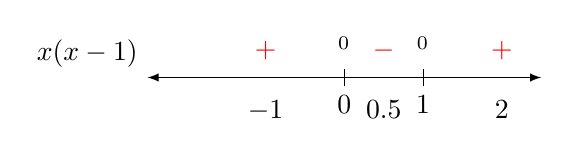
\begin{tikzpicture}
\draw[latex-latex] (-2.5,0) node[above left] {$x(x-1)$} -- (2.5,0) ; %edit here for the axis
%\draw [very thick, - latex, blue] (0,0) -- (2.5,0);
%\node[circle,draw=blue, fill=blue, inner sep=0pt,minimum size=5pt] (a) at (0,0) {};
\foreach \x in  {0,1} % edit here for the vertical lines
\draw[shift={(\x,0)},color=black] (0pt,3pt)  node[above] {$^0$} -- (0pt,-3pt);
\foreach \x in  {0,1}  % edit here for the numbers on vertical lines
\draw[shift={(\x,0)},color=black] (0pt,0pt) -- (0pt,-3pt) node[below] 
{$\x$};
\foreach \x in  {-1,0.5, 2}  % edit here for the numbers below + and -, if desired
\draw[shift={(\x,0)},color=black] (0pt,-5pt) -- (0pt,-5pt) node[below] 
{$\x$};
\foreach \x in  {-1,2}  % edit here for +'s
\draw[shift={(\x,3pt)},color=red] node[above] {$+$};
\foreach \x in  {0.5}  % edit here for -'s
\draw[shift={(\x,3pt)},color=red] node[above] {$-$};
\end{tikzpicture}
\caption{A sign analysis of $x^2-x = x(x-1)$, represented on a number line.}
\label{num:quadsignanalysis}
\end{center}
\end{figure}

From our sign analysis, we see that $x(x-1)$ is positive for $x<0$ and $x>1$, and negative  for $0<x<1$. We wished to find the solution to the inequality
$$x^2-x<0\quad\text{meaning}\quad x(x-1)<0$$
and so we see that the solution is values of $x$ on the interval $0<x<1$, which we write using interval notation as 
$$x\in(0,1).$$
\end{example}

In Example \autoref{ex:quadsignanalysis} above, we can see that the quadratic function $q(x) = x^2-x$ { changes sign} at $x=0$ and $x=1$, where it is equal to zero. Visually, this is where the graph fully crosses the $x$-axis:

\begin{center}
\includegraphics[width=2in]{QuadExample1.png}
\end{center}

As a rule, quadratic functions (and polynomials in general) are only able to change sign only where their graph crosses the $x$-axis:

\begin{theorem}[When Can a Polynomial Change Sign?]\label{thm:polynomialchangesign}
A polynomial can change sign only at values where it is equal to zero. 
\end{theorem}

This theorem is a special case of the Intermediate Value Theorem, which we will explore in Chapter 2. 

\textbf{Important!} 
Just because a polynomial {\it can} change sign does not mean that it {\it does} change sign. The following example illustrates this fact. 


\begin{example}
The quadratic function $q(x) = x^2+2x+1$ factors as $(x+1)(x+1)$ and so has a single zero at $x=-1$ where it can change sign. We test points above and below $x=-1$ to determine the sign of the expression by determining the sign of each factor:

\begin{table}[H]
\centering
\begin{tabular}{c|c|c|c}
\toprule
Interval & Sign of $x+1$ & Sign of $x+1$ & Sign of $(x+1)(x+1)$\\
\hline
$x<-1$ & $-$ & $-$ & $(-)(-)=+$\\
e.g. $x=-2$ & $-2+1 = -1$ & $-2+1 = -1$ & $(-1)(-1) = 1$\\
\hline
$x>-1$ & $+$ & $+$ & $(+)(+)=+$\\
e.g. $x=2$ & $2+1 = 3$ & $2+1 = 3$ & $(3)(3) = 9$\\
\bottomrule
\end{tabular}
\caption{A sign analysis of $x^2+2x+1 = (x+1)(x+1)$.}
\label{tab:posquadsignanalysis}
\end{table}

Summarizing this on a number line:


%%%%%%%%%%%%%%%
%%%%%%%%%Number line
%%%%%%%%%%%%%%%

\begin{figure}[H]
\begin{center}
\begin{tikzpicture}
\draw[latex-latex] (-2.5,0) node[above left] {$(x+1)(x+1)$} -- (2.5,0) ; %edit here for the axis
%\draw [very thick, - latex, blue] (0,0) -- (2.5,0);
%\node[circle,draw=blue, fill=blue, inner sep=0pt,minimum size=5pt] (a) at (0,0) {};
\foreach \x in  {-1} % edit here for the vertical lines
\draw[shift={(\x,0)},color=black] (0pt,3pt)  node[above] {$^0$} -- (0pt,-3pt);
\foreach \x in  {-1}  % edit here for the numbers on vertical lines
\draw[shift={(\x,0)},color=black] (0pt,0pt) -- (0pt,-3pt) node[below] 
{$\x$};
\foreach \x in  {-2,2}  % edit here for the numbers below + and -, if desired
\draw[shift={(\x,0)},color=black] (0pt,-5pt) -- (0pt,-5pt) node[below] 
{$\x$};
\foreach \x in  {-2,2}  % edit here for +'s
\draw[shift={(\x,3pt)},color=red] node[above] {$+$};
%\foreach \x in  {0.5}  % edit here for -'s
%\draw[shift={(\x,3pt)},color=red] node[above] {$-$};
\end{tikzpicture}
\caption{A sign analysis of $x^2+2x+1 = (x+1)(x+1)$, represented on a number line.}
\label{num:posquadsignanalysis}
\end{center}
\end{figure}


We see that despite having an $x$-intercept at $x=-1$, $q(x)=x^2+2x+1$ does not change sign at $x=-1$.  $q(x)$ is positive (meaning $q(x) = x^2+2x+1>0$) on the intervals $(-\infty,-1)\cup(-1,\infty)$, is zero at $x=-1$, and is never negative. You should graph $q(x)$ to confirm. 
\end{example}

\begin{exercise}\label{ex:quadineqmethod}
\textbf{Method for solving quadratic inequalities:} Follow the steps below to determine the intervals where 
$$f(x) = x^2-x-6$$
is positive and negative. 
\begin{enumerate}[label=\alph*., itemsep=5pt,topsep=5pt]
\item Factor $f(x)$ to see that it is equal to zero at $x=-2$ and $x=3$. 
\item Copy the table below to your notes and fill it in, picking suitable values of $x$ on each interval to test the signs of the linear factors of $x^2-x-6$:  $x+\rule[-.25em]{0.15in}{1pt}$ and $x-\rule[-.25em]{0.15in}{1pt}$.

\begin{table}[H]
\centering
\begin{tabular}{c|c|c|c}
\toprule
Interval & Sign of $x-\rule[-.25em]{0.15in}{1pt}$ & Sign of $x+\rule[-.25em]{0.15in}{1pt}$& Sign of $(x-\rule[-.25em]{0.15in}{1pt})(x+\rule[-.25em]{0.15in}{1pt})$\\
\hline
$x<-2$ &  &  & \\
e.g. $x=\rule[-.25em]{0.15in}{1pt}$ &  &  & \\
\hline
$-2<x<3$ &  &  & \\
e.g. $x=\rule[-.25em]{0.15in}{1pt}$ &  &  & \\
\hline
$x>3$ & &  & \\
e.g. $x=\rule[-.25em]{0.15in}{1pt}$ &  &  & \\
\bottomrule
\end{tabular}
\end{table}
\item Summarize your table on a number line, marking where $f(x)=x^2-x-6$ is equal to zero with a tick mark and a 0, positive with a $+$, and negative with a $-$.
\item On what interval(s) is $f(x)=x^2-x-6$ positive? On what interval(s) is $f(x) = x^2-x-6$ negative?
\item Suppose you wanted to find where $g(x) = x^2+1$ is positive and negative, but you discover that $x^2+1=0$ has no solutions. What should you conclude?
\end{enumerate}
\end{exercise}

\fbox{\parbox{5.5in}{
\textbf{Note:} The method outlined in Exercise \ref{ex:quadineqmethod} will be used throughout this course! With enough practice, you will eventually be able to complete a sign analysis with only a number line to keep track of details and will not have to write out the entire table. In fact, by the end of the course, you will likely be able to carry out the majority of Exercise \ref{ex:quadineqmethod} in your head, and in only a fraction of the amount of time it now takes. However, we will continue to provide the full table, along with the sign charts on number lines, throughout the rest of this section while you continue to develop your skills at this method.
}}


\subsubsection{Application: Rewriting a Piecewise-Defined Function by Solving an Inequality}

In this subsection we see how to use inequalities to rewrite functions involving absolute values as piecewise-defined functions. 

\begin{example}
We wish to write $f(x) =  |x^2-1|$ from Exercise \ref{ex:TaalmanSec0.5Ex4} as a piecewise-defined function without needing to rely on a graph of $y=x^2-1$. 

When $x^2-1$ is positive or zero, its absolute value will remain $x^2-1$. When $x^2-1$ is negative, its absolute value will be $-(x^2-1)$. Therefore we have
$$f(x) = |x^2-1| = \begin{cases}
x^2-1, & \text{for all }x\text{ with }x^2-1\geq 0\\
-(x^2-1), & \text{for all }x\text{ with }x^2-1< 0\\
\end{cases}$$

Thus we need to determine where $y=x^2-1$ is positive and negative. For this, we factor and complete a sign analysis:

Since $x^2-1=(x+1)(x-1)=0$ when $x=\pm1$, we  test the sign of $x^2-1$ for $x<-1, -1<x<1,$ and $x>1$:



\begin{table}[H]
\centering
\begin{tabular}{c|c|c|c}
\toprule
Interval & Sign of $x+1$ & Sign of $x-1$ & Sign of $(x+1)(x-1)$\\
\hline
\hline
$x<-1$ & $-$ & $-$ & $(-)(-)=+$\\
e.g. $x=-2$ & $-2+1=-1$ & $-2-1 = -3$ & $(-1)(-3) = 3$ \\
\hline
$-1<x<1$ & $+$ & $-$ & $(+)(-)=-$\\
e.g. $x=0$ & $0+1=1$ & $0-1 = -1$ & $(1)(-1) = -1$\\
\hline
$x>1$ & $+$ & $+$ & $(+)(+)=+$\\
e.g. $x=2$ & $2+1=3$ & $2-1 = 1$ & $(3)(1) = 3$\\
\bottomrule
\end{tabular}
\caption{A sign analysis of $x^2-1 = (x+1)(x-1)$.}
\label{tab:absvalquadsignanalysis}
\end{table}


Summarizing this on a number line:


%%%%%%%%%%%%%%%
%%%%%%%%%Number line
%%%%%%%%%%%%%%%

\begin{figure}[H]
\begin{center}
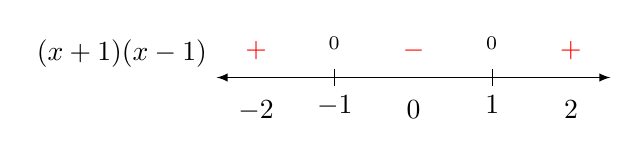
\begin{tikzpicture}
\draw[latex-latex] (-2.5,0) node[above left] {$(x+1)(x-1)$}  -- (2.5,0) ; %edit here for the axis
%\draw [very thick, - latex, blue] (0,0) -- (2.5,0);
%\node[circle,draw=blue, fill=blue, inner sep=0pt,minimum size=5pt] (a) at (0,0) {};
\foreach \x in  {-1,1} % edit here for the vertical lines
\draw[shift={(\x,0)},color=black] (0pt,3pt)  node[above] {$^0$} -- (0pt,-3pt);
\foreach \x in  {-1,1}  % edit here for the numbers on the vertical lines
\draw[shift={(\x,0)},color=black] (0pt,0pt) -- (0pt,-3pt) node[below] 
{$\x$};
\foreach \x in  {-2,0,2}  % edit here for the numbers below + and -, if desired
\draw[shift={(\x,0)},color=black] (0pt,-5pt) -- (0pt,-5pt) node[below] 
{$\x$};
\foreach \x in  {-2,2}  % edit here for +'s
\draw[shift={(\x,3pt)},color=red] node[above] {$+$};
\foreach \x in  {0}  % edit here for -'s
\draw[shift={(\x,3pt)},color=red] node[above] {$-$};
\end{tikzpicture}
\end{center}
\caption{A sign analysis of $x^2-1 = (x+1)(x-1)$, represented on a number line.}
\label{num:absvalquadsignanalysis}
\end{figure}

We see that $x^2-1 = (x+1)(x-1)$ is positive on $(-\infty,-1)\cup(1,\infty)$ and negative on $(-1,1)$. Thus we have
$$f(x) = |x^2-1| = \begin{cases}
x^2-1, & \text{if } x\leq -1 \text{ or } x\geq 1\\
-(x^2-1), &  \text{if } -1<x<1
\end{cases}$$

%You should take a moment to use this formula to check your answers to Example \ref{ex:TaalmanSec0.5Ex4}. 
%
%The graph of $y=|x^2-1|$ is the same as the graph of $y=x^2-1$ on the intervals $(-\infty,-1]$ and $[1,\infty)$. On the interval $(-1,1)$, the quantity $|x^2-1|$ has the sign opposite that of $x^2-1$, so its graph is the reflection of the negative parts of $x^2-1$ across the $x$-axis, as the following figure shows:
%
%\begin{center}
%\includegraphics[width=2in]{TaalmanPage59.png}
%\end{center}
\end{example}



\subsection{Solving Inequalities That Involve Products and Quotients}




Recall Theorem \ref{thm:signofproducts}: The Sign of a Product $AB$ Depends on the Signs of its Factors.  This theorem also holds for quotients: $\frac{A}{B}$ is greater than zero if $A$ and $B$ have the same sign and is less than zero if $A$ and $B$ have opposite signs. We can also generalize this theorem to products with more than two factors:

\begin{theorem}[The Sign of a Product or Quotient Depends on the Number of Its Negative Factors]\label{thm:gensignofproduct}
A product or quotient of nonzero real numbers is positive if and only if it has an even number of negative factors and is negative if and only if it has an odd number of negative factors. 
\end{theorem}

For example, the product $(-2)(-1)(2)(-6)$ is negative because it has an odd number of negative factors. In contrast, $\frac{(-3)(-2)(-8)}{(7)(-4)}$ is positive because it has an even number of negative factors. 




\begin{example}
As an illustration of the power of Theorem \ref{thm:gensignofproduct}, consider the problem of solving the inequality 
$$(x^2+2)(x+1)(x-1)<0.$$

 Applying  Theorem \ref{thm:quotientchangesign}, the expression $(x^2+2)(x+1)(x-1)$ is zero only when $x=-1$ and $x=1$. (Note that $x^2+2$ is never zero; it is irreducible.) Therefore, these are the only two $x$-values at which the expression can change sign. That means that the expression has the same sign on the entire interval $(-\infty, -1)$, and the same sign on all of $(-1,1)$, and the same sign on all of $(1,\infty)$. Applying Theorem \ref{thm:gensignofproduct}, we can test the sign of each factor and multiply to find the sign of the entire product:

\begin{table}[H]
\centering
\begin{tabular}{c|c|c|c|c}
\toprule
Interval & Sign of $x^2+2$ & Sign of $x+1$ & Sign of $x-1$ & Sign of $(x^2)(x+1)(x-1)$\\
\hline
\hline
$x<-1$ & $+$ & $-$ & $-$ &  $(+)(-)(-)=+$\\
e.g. $x=-2$ & $(-2)^2+2=6$ & $-2+1 = -1$ & $-2-1 = -3$ &$(6)(-1)(-3) = 18$ \\
\hline
$-1<x<1$ & $+$ & $+$ & $-$ & $(+)(+)(-)=-$\\
e.g. $x=0$ & $(0)^2+2=2$ & $0+1 = 1$ & $0-1 = -1$ &$(2)(1)(-1) = -2$ \\
\hline
$x>1$ & $+$ & $+$ & $+$ & $(+)(+)(+)=+$\\
e.g. $x=2$ & $(2)^2+2=6$ & $2+1 = 3$ & $2-1 = 1$ &$(6)(3)(1) = 18$ \\
\bottomrule
\end{tabular}
\caption{A sign analysis of $(x^2+2)(x+1)(x-1)$.}
\label{tab:quarticsignanalysis}
\end{table}

Summarizing this on a number line:


%%%%%%%%%%%%%%
%%%%%%%%Number line
%%%%%%%%%%%%%%
\begin{figure}[H]
\begin{center}
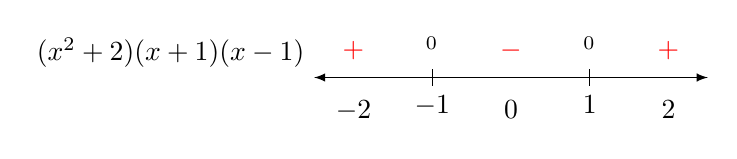
\begin{tikzpicture}
\draw[latex-latex] (-2.5,0) node[above left] {$(x^2+2)(x+1)(x-1)$} -- (2.5,0) ; %edit here for the axis
%\draw [very thick, - latex, blue] (0,0) -- (2.5,0);
%\node[circle,draw=blue, fill=blue, inner sep=0pt,minimum size=5pt] (a) at (0,0) {};
\foreach \x in  {-1,1} % edit here for the vertical lines
\draw[shift={(\x,0)},color=black] (0pt,3pt)  node[above] {$^0$} -- (0pt,-3pt);
\foreach \x in  {-1,1}  % edit here for the numbers on the vertical lines
\draw[shift={(\x,0)},color=black] (0pt,0pt) -- (0pt,-3pt) node[below] 
{$\x$};
\foreach \x in  {-2, 0,2}  % edit here for the numbers below + and -, if desired
\draw[shift={(\x,0)},color=black] (0pt,-5pt) -- (0pt,-5pt) node[below] 
{$\x$};
\foreach \x in  {-2,2}  % edit here for +'s
\draw[shift={(\x,3pt)},color=red] node[above] {$+$};
\foreach \x in  {0}  % edit here for -'s
\draw[shift={(\x,3pt)},color=red] node[above] {$-$};
\end{tikzpicture}
\end{center}
\caption{A sign analysis of $(x^2+2)(x+1)(x-1)$, represented on a number line.}
\label{num:quarticsignanalysis}
\end{figure}

From this, we can conclude that $(x^2+2)(x+1)(x-1)$ is less than zero exactly when $x\in(-1,1)$, and we have solved the inequality. 
\end{example}


There is also a version of Theorem \ref{thm:polynomialchangesign} that holds for rational functions:

\begin{theorem}[When Can a Quotient of Polynomials Change Sign?]\label{thm:quotientchangesign}
A quotient of polynomials can change sign only at values where its numerator or denominator is equal to zero. 
\end{theorem}

The next example applies this theorem to solving an inequality involving a rational function. 

\begin{example}\label{ex:signofquotient}
Determine where 
$$h(x) = \frac{1-2x}{x+1}$$
is positive and negative.

\begin{solution}
The expression $\frac{1-2x}{x+1}$ can change sign only when either the numerator or denominator is equal to zero, by Theorem \ref{thm:quotientchangesign}. 
$$\text{The numerator}\quad 1-2x = 0\quad\text{when}\quad x=\frac{1}{2}$$
and 
$$\text{the denominator}\quad x+1 = 0\quad\text{when}\quad x=-1.$$
Thus we perform a sign analysis on the intervals $(-\infty,-1)$, $\left(-1,\frac{1}{2}\right)$, and $\left(\frac{1}{2},\infty\right)$, testing the sign of each factor in the numerator and denominator and combining to determine the sign of the quotient according to Theorem \ref{thm:gensignofproduct}.

\begin{table}[H]
\centering
\begin{tabular}{c|c|c|c}
\toprule
Interval & Sign of $1-2x$ & Sign of $x+1$ & Sign of $\frac{1-2x}{x+1}$\\
\hline
\hline
$x<-1$ & $+$ & $-$ & $\dfrac{+}{-}=-$\\
e.g. $x=-2$ & $1-2(-2)=5$ & $-2+1 = -1$ & $\frac{5}{-1}=-5$ \\
\hline
$-1<x<\frac{1}{2}$ & $+$ & $+$ & $\dfrac{+}{+}=+$\\
e.g. $x=0$ & $1-2(0)=1$ & $0+1 = 1$ & $\frac{1}{1}=1$\\
\hline
$x>\frac{1}{2}$ & $-$ & $+$ & $\dfrac{-}{+}=-$\\
e.g. $x=2$ & $1-2(2) =-3$ & $2+1 = 3$ & $\frac{-3}{3}=-1$\\
\bottomrule
\end{tabular}
\caption{A sign analysis of $\frac{1-2x}{x+1}$.}
\label{tab:quotientsignanalysis}
\end{table}

Summarizing this on a number line:


%%%%%%%%%%%%%%%
%%%%%%%%%Number line
%%%%%%%%%%%%%%%

\begin{figure}[H]
\begin{center}
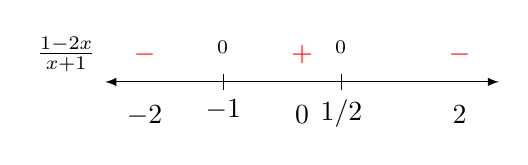
\begin{tikzpicture}
\draw[latex-latex] (-2.5,0) node[above left] {$\frac{1-2x}{x+1}$}  -- (2.5,0) ; %edit here for the axis
%\draw [very thick, - latex, blue] (0,0) -- (2.5,0);
%\node[circle,draw=blue, fill=blue, inner sep=0pt,minimum size=5pt] (a) at (0,0) {};
\foreach \x in  {-1,0.5} % edit here for the vertical lines
\draw[shift={(\x,0)},color=black] (0pt,3pt)  node[above] {$^0$} -- (0pt,-3pt);
\foreach \x in  {-1,1/2}  % edit here for the numbers on the vertical lines
\draw[shift={(\x,0)},color=black] (0pt,0pt) -- (0pt,-3pt) node[below] 
{$\x$};
\foreach \x in  {-2,0,2}  % edit here for the numbers below + and -, if desired
\draw[shift={(\x,0)},color=black] (0pt,-5pt) -- (0pt,-5pt) node[below] 
{$\x$};
\foreach \x in  {0}  % edit here for +'s
\draw[shift={(\x,3pt)},color=red] node[above] {$+$};
\foreach \x in  {-2,2}  % edit here for -'s
\draw[shift={(\x,3pt)},color=red] node[above] {$-$};
\end{tikzpicture}
\end{center}
\caption{A sign analysis of $\frac{1-2x}{x+1}$, represented on a number line.}
\label{num:quotientsignanalysis}
\end{figure}


So we see that $h(x) = \frac{1-2x}{x+1}$ is positive on $\left(-1,\frac{1}{2}\right)$ and negative on $(-\infty,-1)\cup \left(\frac{1}{2},\infty\right)$.
\end{solution}

\end{example}


In the next example, we see how to solve an inequality where neither side is 0: we must rewrite the inequality so that one side \textit{is} 0 and then perform a sign analysis. This requires further simplifying the nonzero expression to be a quotient of fully factored expressions. 

\begin{example}\label{ex:nonzeroineq}
Solve the inequality 
$$\frac{3}{x+1}\geq 2$$

\end{example}

\begin{solution}
Although it is tempting, recall that we can't multiply both sides of the inequality by $x+1$ because $x+1$ may be positive or may be negative (depending on the value of $x$). Instead, we will use some algebra to turn this inequality into one that involves a product or quotient of factors on one side and zero on the other:

$$\begin{aligned}
\frac{3}{x+1} &\geq2 & \quad& \leftarrow \text{ original inequality}\\
\frac{3}{x+1}-2 &\geq 0 & \quad& \leftarrow \text{ collect terms so 0 is on the right-hand side}\\
\frac{3}{x+1}-\frac{2(x+1)}{x+1}&\geq 0 & \quad& \leftarrow \text{find common denominator}\\
\frac{3-2(x+1)}{x+1}&\geq 0 & \quad& \leftarrow \text{combine fractions}\\
\frac{3-2x-2}{x+1}&\geq 0 & \quad& \leftarrow \text{simplify numerator}\\
\frac{1-2x}{x+1}&\geq 0 & \quad& \leftarrow \text{simplify numerator some more}\\
\end{aligned}$$

Note that none of the above steps has changed the values of $x$ that can satisfy the inequalities. In other words, the inequality $\frac{3}{x+1} \geq2$ has the same solution set as the inequality $\frac{1-2x}{x+1}\geq 0 $. 

Notice that the latter inequality $\frac{1-2x}{x+1}\geq 0 $ is now a problem we have already solved! In Example \autoref{ex:signofquotient}, we found that the function $h(x) = \frac{1-2x}{x+1}$ is positive for $x\in \left(-1,\frac{1}{2}\right)$. Additionally, the fraction $\frac{1-2x}{x+1}$ is equal to zero when its numerator is zero, so for $x = \frac{1}{2}$. Thus 
$$\frac{1-2x}{x+1}\geq 0 \quad\text{for}\quad x\in  \left(-1,\frac{1}{2}\right].$$
Remembering that the two inequalities have the same solution sets, we realize that we have now solved the original problem, and conclude
$$\frac{3}{x+1}\geq 2\quad\text{for}\quad x\in  \left(-1,\frac{1}{2}\right].$$

\end{solution}



\begin{exercise}
Why is the square bracket used for the endpoint $x=\frac{1}{2}$ in Example \autoref{ex:nonzeroineq} but not the endpoint $x=-1$?
\end{exercise}

%\begin{exercise}
%Use point testing and a sign chart to find the solution set of the inequality $\frac{1}{x-2}\leq \frac{1}{6-x}$, as demonstrated above. {\it Start by moving everything to one side of the inequality so that one side is 0, combine fractions and factor the numerator and denominator, then test points for the signs of the factors.} 
%\end{exercise}


\subsubsection{Application: Finding the Domain of a Function with an Even Root}


%From Taalman Section 0.4 Example 5
\begin{example}
Find the domain of the algebraic function
$$f(x) = \sqrt{\frac{3}{x}-2}$$
\end{example}

%\todo{return to $\frac{3}{x}>2$}

\begin{solution}
To find the domain of $f$, we ask which values of $x$ can be plugged into the equation that defines $f(x)$ and produce a real number when the expression is simplified. In order for the value of $f$ to be defined for a real number $x$, that value of $x$ must make the expression underneath the square-root sign nonnegative (meaning $\frac{3}{x}-2\geq 0$) and the denominator appearing in $\frac{3}{x}$ nonzero (meaning $x\neq 0$). Thus the domain of $f(x)$ is the set of real numbers that satisfy:
$$\frac{3}{x}-2\geq 0\quad\text{and}\quad x\neq 0$$

In order to tackle the inequality, we need to rewrite the left-hand side as a single fraction:
$$\begin{aligned}
\frac{3}{x}-2 &\geq 0& \quad& \leftarrow \text{ original inequality}\\
\frac{3}{x}-\frac{2x}{x} &\geq 0 & \quad& \leftarrow \text{find common denominator}\\
\frac{3-2x}{x}&\geq 0 & \quad& \leftarrow \text{combine fractions}\\
\end{aligned}$$

The fraction can change sign when the numerator is zero:
$$3-2x=0\quad\text{when}\quad x=\frac{3}{2}$$
or when the denominator is zero:
$$x=0.$$
Performing a sign analysis for $\frac{3-2x}{x}$:


\begin{table}[H]
\centering
\begin{tabular}{c|c|c|c}
\toprule
Interval & Sign of $3-2x$ & Sign of $x$ & Sign of $\frac{3-2x}{x}$\\
\hline
\hline
$x<0$ & $+$ & $-$ & $\dfrac{+}{-}=-$\\
e.g. $x=-1$ & $3-2(-1)=5$ & $-1$ & $\frac{5}{-1}=-5$ \\
\hline
$0<x<\frac{3}{2}$ & $+$ & $+$ & $\dfrac{+}{+}=+$\\
e.g. $x=1$ & $3-2(1)=1$ & $ 1$ & $\frac{1}{1}=1$\\
\hline
$x>\frac{3}{2}$ & $-$ & $+$ & $\dfrac{-}{+}=-$\\
e.g. $x=2$ & $3-2(2)=-1$ & $ 2$ & $\frac{-1}{2}=-\frac{1}{2}$\\
\bottomrule
\end{tabular}
\caption{A sign analysis of $\frac{3-2x}{x}$.}
\label{tab:anotherquotientsignanalysis}
\end{table}



Summarizing this on a number line: 

%%%%%%%%%%%%%%
%%%%%%%%Number line
%%%%%%%%%%%%%%
\begin{figure}[H]
\begin{center}
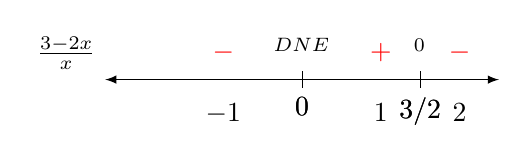
\begin{tikzpicture}
\draw[latex-latex] (-2.5,0) node[above left] {$\frac{3-2x}{x}$} -- (2.5,0) ; %edit here for the axis
%\draw [very thick, - latex, blue] (0,0) -- (2.5,0);
%\node[circle,draw=blue, fill=blue, inner sep=0pt,minimum size=5pt] (a) at (0,0) {};
\foreach \x in  {0, 3/2} % edit here for the vertical lines
\draw[shift={(\x,0)},color=black] (0pt,3pt) -- (0pt,-3pt);
\foreach \x in  {0,3/2}  % edit here for the numbers on the vertical lines
\draw[shift={(\x,0)},color=black] (0pt,0pt) -- (0pt,-3pt) node[below] 
{$\x$};
\foreach \x in  {0,3/2}  % edit here for the numbers on the vertical lines
\draw[shift={(\x,0)},color=black] (0pt,0pt) -- (0pt,-3pt) node[below] 
{$\x$};
\foreach \x in  {-1,1,2}  % edit here for the numbers below + and -, if desired
\draw[shift={(\x,0)},color=black] (0pt,-5pt) -- (0pt,-5pt) node[below] 
{$\x$};
\foreach \x in  {3/2}  % edit here for 0's
\draw[shift={(\x,3pt)}] node[above] {$^0$};
\foreach \x in  {0}  % edit here for DNE's
\draw[shift={(\x,3pt)}] node[above] {$^\text{DNE}$};
\foreach \x in  {1}  % edit here for +'s
\draw[shift={(\x,3pt)},color=red] node[above] {$+$};
\foreach \x in  {-1,2}  % edit here for -'s
\draw[shift={(\x,3pt)},color=red] node[above] {$-$};
\end{tikzpicture}
\end{center}
\caption{A sign analysis of $\frac{3-2x}{x}$, represented on a number line.}
\label{num:anotherquotientsignanalysis}
\end{figure}


Thus $\frac{3-2x}{x}$ is positive on $\left(0,\frac{3}{2}\right)$, and we know that it is equal to zero at $x=\frac{3}{2}$; it is undefined at $x=0$. The equivalent inequality $\frac{3}{x}-2\geq 0$ thus has solution $\left(0,\frac{3}{2}\right]$. Note that the second condition, $x\neq 0$, on the domain is also satisfied. 

Hence overall we have found the domain of the function $f(x) = \sqrt{\frac{3}{x}-2}$ by determining that $\frac{3}{x}-2\geq 0$ and $x\neq 0$ on the interval 
$$\left(0,\frac{3}{2}\right].$$


%The only $x$-values at which the quotient in the inequality can change sign are $x=\frac{1}{2}$ and $x=-1$, since those are the values that make either the numerator or denominator equal to zero. To determine the intervals on which the quotient is positive or negative we need only check its sign between the possible change points $x=\frac{1}{2}$ and $x=-1$. 
%
%We can record this information on a number line with a {\bf sign chart} as follows:
%
%
%


\end{solution}





\subsection*{Summary}
The following terms and methods were introduced in this section: 
\begin{quotation}
inequality, solution set, sign analysis of products and quotients. 
\end{quotation}

\textbf{Key ideas:} The solutions of inequalities are intervals of numbers. Multiplying or dividing an inequality by a negative number requires flipping the inequality. The sign of a product or quotient depends on the number of its negative factors. A polynomial can only change sign where it is equal to zero. A quotient of polynomials can only change sign where its numerator or denominator is equal to zero. In order to solve an inequality involving a product or quotient, algebraically manipulate the inequality so that one side is 0, then perform a sign analysis on the nonzero side. 

\textbf{Other ideas reinforced:} Finding the domain of a function with an even root can involve solving an inequality. Writing a function involving an absolute value as a piecewise-defined function can involve solving an inequality. 



\begin{center}
\textcolor{ocre}{\fbox{\fbox{\Large \bf \sc End of Section 1.8}}}
\end{center}

\hspace{-.5in}\rule{1.1\textwidth}{2pt}






\section{Composition of Functions}\index{Functions!Composition of Functions}


\subsection*{Learning Goals}
\begin{itemize}
	\item Understand what it means to compose two functions
	\item Calculate values of compositions of functions given tables, graphs, or formulas
	\item Simplify the formula for a composition of functions
	\item Determine the domain of a composition of functions
	\item See an example where composition of functions is vital to studying calculus
\end{itemize}


\subsection{Motivation and Examples}

%APC Section 1.6
Recall that a function, by definition, is a process that takes a collection of inputs and produces a corresponding collection of outputs in such a way that the process produces one and only one output value for any single input value. Because every function is a process, it makes sense to think that it may be possible to take two function processes and do one of the processes first, and then apply the second process to the result.


Recall Dolbear's function, $F=D(N)=40+0.25N$, from Example \autoref{ex:DolbearTake1} that relates the number $N$ of chirps per minute from a snowy cricket to the Fahrenheit temperature, $F$. 

The Celsius and Fahrenheit temperature scales are connected by a linear function. Indeed, the function that converts Fahrenheit to Celsius is
$$C = G(F) = \frac{5}{9}(F-32).$$

For instance, a Fahrenheit temperature of 32 degrees corresponds to $C=G(32) = 0$ degrees Celsius. 

If we are given a number of chirps, $N$, we can combine the two processes given by Dolbear's function and the conversion from Fahrenheit to Celsius to obtain a new function $C=H(N)$ that takes as input the number of chirps per minute and gives as output the temperature in degrees Celsius. 

\begin{example}
Suppose that we observe 80 chirps per minute. What is the temperature in degrees Celsius?

First, we compute that the temperature in degrees Fahrenheit is
$$F = D(80) = 40+0.25(80) = 60.$$
Then, we compute that the temperature in degrees Celsius is
$$C = G(60) = \frac{5}{9}(60-32) = \frac{140}{9} =15\frac{5}{9}^\circ C.$$
\end{example}

We could do this individually for each value of $N$, but it would be more convenient to have a single formula that can go directly from number of chirps per minute to degrees Celsius. In the above example, we took the output $F=D(80)$ and used it as the input for the temperature conversion $C=G(F)$ from Fahrenheit to Celsius. We can do the same thing using the variable $N$ instead of the explicit input $N=80$:

\begin{example}
Determine a formula for the new function $C=H(N)$ that takes as input the number $N$ of cricket chirps per minute and gives as output the temperature $C$ in degrees Celsius. 

Using $F=D(N)$ as the input for the function $C=G(F)$, we simplify to find a formula directly from $N$ to $C$ that does not involve the variable $F$:
$$\begin{aligned}
C &= G(F)\\
&= G(D(N))\\
&= \frac{5}{9}(D(N)-32)\\
&= \frac{5}{9}((40+0.25N)-32)\\
&=\frac{5}{9}(8+0.25N)
\end{aligned}$$
So the function $C=H(N)$ is given by
$$C = \frac{5}{9}(8+0.25N).$$
\end{example}

There is, of course, a shorthand notation for this process of using the output of $D$ as the input of $G$:
$$H=G\circ D$$

$G\circ D$ is the function that  first applies the process given by the function $D$ and then applies the process given by the function $G$. Two natural questions we could begin by asking are:
\begin{quotation}
"What is the domain of $H = G\circ D$?" \quad and \quad "What is the range of $H=G\circ D$?"
\end{quotation}

\begin{example}
Find the domain and range of the function $C=H(N)$. 

We established in Example \autoref{ex:DolbearTake2} that $F=D(N)$ has a domain of $[40,180]$ cricket chirps per minute and a corresponding range of $[50,85]$ degrees Fahrenheit. 


The domain for $H=G\circ D$ is the inputs of $H$, so is also the inputs of $D$ as that is the function that is applied first. Thus we can use the same set of $N$-values and the domain of $H$ is also $[40,180]$. 

In order to determine the range, we must find the resulting degrees Celsius from the range of degrees Fahrenheit of $[50,85]$. $$G(50) = \frac{5}{9}(50-32) = 10$$ and $$G(85) = \frac{5}{9}(85-32) = \frac{265}{9}= 29\frac{4}{9}.$$
We know that a linear function's range will stay within these two values based on the shape of the graph. Thus the range of $H$ is in degrees Celsius instead of Fahrenheit, and is $[10,29\frac{4}{9}]$. 

\end{example}



%\todo{Try to find a real-world situation (maybe Dolbear?) that's a better example of this. Cost and demand would be good. Originally have $C(q)$ where $q$ is the quantity, but also have demand function $q(p)$ where $p$ is the price. Can rewrite the cost in terms of price. Pull ideas from HH 4.4}



\subsection{Definition of Composition of Functions}


Suppose we have two function, $g$ and $f$. $g$ has domain $A$ and range $B$, while $f$ has domain $B$ and range $C$. We write $g$ and $f$ along with their domains and ranges as $g:A\to B$ and $f:B\to C$. As long as the range of $g$ matches the domain of $f$, it is possible to link the two processes together to create a new process that we call the \textbf{composition of $f$ and $g$}. 

\begin{definition}[The Composition of Two Functions]
If $f$ and $g$ are functions such that  $g:A\to B$ and $f:B\to C$, we define the \textbf{composition of $f$ and $g$} to be the new function $h:A\to C$ given by
$$h(t) = f(g(x)).$$
We also sometimes use the notation $h = f\circ g$, where $f\circ g$ is the single function defined by 
$$(f\circ g)(x) = f(g(x)).$$ 
 
\end{definition}



\begin{figure}[H]
\centering
\includegraphics[width=5in]{CompositionOfFunctions.png}
\caption{The composition $(f\circ g)(x) = f(g(x))$ uses the outputs $g(x)$ as the inputs of $f$.}
\label{fig:comositionoffunctions}
\end{figure}



We sometimes call $g$ the “inner function” and $f$ the “outer function”. It is important to note that the inner function is actually the first function that gets applied to a given input, and then outer function is applied to the output of the inner function. In addition, in order for a composite function to make sense, we need to ensure that the range of the inner function lies within the domain of the outer function so that the resulting composite function is defined at every possible input.

%In addition to the possibility that functions are given by formulas, functions can be given by tables or graphs. We can think about composite functions in these settings as well, and the following activities prompt us to consider functions given in this way.

In the following examples, we consider compositions of functions given by tables, then by graphs, and finally by formulas. 


\begin{example}\label{ex:compositionbytables}
Suppose that  $f$ and $g$ are given by the table

\begin{center}
\includegraphics[width=1.5in]{APCTable1-6-3.png}
\end{center}

This means, for example, that $f(0)=6$, $f(1)=4$, $f(2) = 3$, etc., and that $g(0)=1, g(1)=3, g(2)=0$, etc. 

 We can calculate $(f\circ g)(2) = f(g(2))$. Since $g(2) = 0$ and $f(0) = 6$, $f(g(2)) = f(0) = 6$. 
 
We can also calculate $(g\circ f)(2) = g(f(2))$. Since $f(2) = 3$ and $g(3)=4$, $g(f(2)) = 4$. 
\end{example}

\begin{exercise}
For $f$ and $g$ as in Example \autoref{ex:compositionbytables}, compute each of the following quantities or explain why they are not defined. 

\begin{enumerate}[label=\alph*.]
\item $(g\circ f)(3)$
\item $g(f(0))$
\item For what value(s) of $x$ is $f(g(x))=4$?
\end{enumerate}
\end{exercise}

\begin{example}\label{ex:compositionbygraphs}
If $p$ and $q$ are given by the graphs

\begin{center}
\includegraphics[width=2.7in]{APCFigure1-6-4.png}
\end{center}

then $(p\circ q)(0) = p(q(0))$. Since $q(0) = 2$ and $p(2) = 2$, $p(q(0)) = p(2) = 2$. 
\end{example}

\begin{exercise}
For $p$ and $q$ as in Example \autoref{ex:compositionbygraphs}, compute each of the following quantities or explain why they are not defined. 

\begin{enumerate}[label=\alph*.]
\item $(q\circ p)(0)$
\item $(p\circ p)(-1.5)$
\item $(q\circ p)(2)$
\end{enumerate}
\end{exercise}





\begin{example}\label{ex:compositionbyformulas}
Suppose that
$$f(x) = x^2-1$$
and that 
 $$g(x) = 3x-\frac{4}{x}$$
 
 The composition $f\circ g$ means that we use $g(x)$ as the inputs for the function $f$. Think of $f$ as the process that squares its input, then subtracts 1:
 $$f(?) = (?)^2-1$$
 If the input is $g(x) = 3x-\frac{4}{x}$, we can simplify: 
 $$\begin{aligned}
 (f\circ g)(x) &= f(g(x))\\
 &= (g(x))^2-1\\
 &= \left(3x-\frac{4}{x}\right)^2-1
 \end{aligned}$$
 We could simplify this further if we wanted to, thought it isn't really necessary:
 $$\begin{aligned}
  (f\circ g)(x) &= \left(3x-\frac{4}{x}\right)^2-1\\
  &= \left(9x^2-24+\frac{16}{x^2}\right)-1\\
  &= 9x^2+\frac{16}{x^2}-25
  \end{aligned}$$
  
We could also compose the other direction. The composition $g\circ f$ means that we use $f(x)$ as the inputs for the function $g$. Think of $g$ as the function that multiplies 3 times its input, divides 4 by its input, then subtracts the latter from the former:
$$g(?) = 3(?)-\frac{4}{?}$$
If the input is $f(x) = x^2-1$, 
$$\begin{aligned}
(g\circ f)(x) &= g(f(x))\\
&= 3(f(x))-\frac{4}{f(x)}\\
&= 3(x^2-1)-\frac{4}{x^2-1}
\end{aligned}$$
We could simplify a littler further if we wanted to by distributing the 3, but anything farther would be a waste of time (like writing it as a single fraction over a common denominator):
$$\begin{aligned}
(g\circ f)(x) &= 3(x^2-1)-\frac{4}{x^2-1}\\
&= 3x^2-3-\frac{4}{x^2-1}
\end{aligned}$$

 
%It is possible to combine these processes to generate a new function so that $y$ is a function of $t$. 
%
%Since $y$ depends on $x$ and $x$ depends on $t$, it follows that we can also think of $y$ depending directly on $t$. We can use substitution and the notation of functions to determine this relationship. 
%
%First, it's important to realize what the rule for $f$ tells us. In words, $f$ says "to generate the output that corresponds to an input, take the input and square it, and then subtract 1." In symbols, we might express $f$ more generally by writing
%$$f(?) = (?)^2-1$$
%
%Now, observing that $y=f(x) = x^2-1$ and that $x=g(t)=3t-4$, we can substitute the expression $g(t)$ for $x$ in $f$. Doing so, 
%$$\begin{aligned}
%y &= f(x)\\
%&= f(g(t))\\
%&= f(3t-4).
%\end{aligned}$$
%
%Applying the process defined by the function $f$ to the input $3t-4$, we see that
%$$y=(3t-4)^2-1$$
%which defines $y$ as a function of $t$. 
\end{example}

%When we have a situation such as in this example where we use the output of one function as the input of another, we often say that we have “composed two functions”. In addition, we use the notation $h(t) = f(g(t))$ to denote that a new function, $h$, results from composing the two functions $f$ and $g$. 


\begin{exercise}\label{ex:compositionbyformulas2}
Let $p(x) = \frac{1}{x+4}$ and $q(x) = x^2-4$. 

\begin{enumerate}[label=\alph*.]
\item Find and simplify (as much as is reasonable) a formula for $p\circ q$. 
\item Find and simplify (as much as is reasonable) a formula for $q\circ p$. 
\end{enumerate}
\end{exercise}


\begin{example}
Suppose that $h(x) = \sqrt{2x^2+5}$. Determine formulas for two related functions, $f(x)$ and $g(x)$, so that $h(x) = f(g(x))$. 
\end{example}

\begin{solution}
One possibility is that $f(x) = \sqrt{x}$ and $g(x) = 2x^2+5$. 

Another possibility is that $f(x) = \sqrt{2x+5}$ and $g(x) = x^2$. 

Do you see any additional possibilities?
\end{solution}



\fbox{\parbox{5.5in}{
\textbf{Important!} 
Function composition is \textbf{not at all} like multiplication. As we have seen in Example \autoref{ex:compositionbyformulas} and Exercise \autoref{ex:compositionbyformulas2}, it is not necessarily true that $f\circ g = g\circ f$ or that $p\circ q = q\circ p$. In fact, that is usually not true at all. 
}}




\subsection{Domain of Compositions}

%Stewart Section 1.3
Suppose we have two functions, $y=f(x)$ and $x=g(t)$. The domain of $f\circ g$ is the set of all $t$ in the domain of $g$ such that $x=g(t)$ is in the domain of $f$. In other words, $(f\circ g)(t)$ is defined whenever both $g(t)$ and $f(g(t))$ are defined. 

%Taalman Section 0.6 Example 1 parts d and e
\begin{example}
For $y=f(x) = \frac{1}{x}$ and $x=g(t) = \sqrt{t+1}$, we find the domain of $f\circ g$. 

For a value $t$ to be in the domain of $f\circ g$, it must first be in the domain $[-1,\infty)$ of $g$. Then the value of $g(t) = \sqrt{t+1}$ must be in the domain of $f$, so we must have $\sqrt{t+1}\neq 0$, or in other words, $t\neq 1$. Therefore the domain of $f\circ g$ is $(-1,\infty)$. 

For values of $t$ in this domain, we have 
$$(f\circ g)(t) = f(g(t)) = f(\sqrt{t+1}) = \frac{1}{\sqrt{t+1}}.$$
Notice that this equation is consistent with our calculation of the domain. 
\end{example}


\begin{exercise}
For $y=g(x) =\sqrt{x+1}$ and $x=f(t) = \dfrac{1}{t}$, find the domain of $g\circ f$. 
\end{exercise}


\begin{example}
Recall the functions $f(x) = x^2-1$
and  
 $g(x) = 3x-\frac{4}{x}$ from Example \autoref{ex:compositionbyformulas}. Let's find the domains of $f\circ g$ and $g\circ f$. 
 
The domain of $g(x)$ is $x\neq 0$. The domain of $f(x)$ is all real numbers, so there is no need to limit the outputs of $g$. Hence the domain is $(-\infty,0)\cup (0,\infty)$. We found a simplified formula of 
 $$(f\circ g)(x) = 9x^2+\frac{16}{x^2}-25,$$
which agrees with our previous analysis. 

In the other direction, the domain of $f(x) = x^2-1$ has no restrictions, but when we plug $f(x)$ into $g(x) = 3x-\frac{4}{x}$, we notice that this requires the input to be nonzero because of the $x$ in the denominator, hence we must have $f(x) = x^2-1\neq 0$ in order for $g(f(x))$ to be defined. Thus the domain for $g\circ f$ should be $x\neq \pm1$. Indeed, we found a simplified formula of
$$(g\circ f)(x) = 3x^2-3-\frac{4}{x^2-1}$$
Since $x^2-1$ is in the denominator, we cannot have $x=1$ or $x=-1. $ Thus the domain is indeed $(-\infty,-1)\cup(-1,1)\cup(1,\infty)$. 
\end{example}


\begin{example}[A Cautionary Example]
Let's consider the functions $f(x) =g(x) =  \frac{1}{x}$ and look at the domain of $f\circ g$. If we view $g(x)$ as the first function applied to $x$, we know that we must have $x\neq 0$. 

However, if we first simplify the formula for the composition:
$$\begin{aligned}
(f\circ g)(x) &= f(g(x))\\
&= \frac{1}{g(x)}\\
&=\frac{1}{1/x}\\
&= x
\end{aligned}$$
we might think that the domain is all real numbers, which would be incorrect!
\end{example}

\fbox{\parbox{5.5in}{
\textbf{Remember!} The domain of $(f\circ g)(x)$ is the values of $x$ in the domain of $g$ so that the output of $g(x)$ is \textit{also} in the domain of $f$.
}}

\subsection{Function Composition and Average Rate of Change}

In this section, we see how the idea of composition can be used in concert with the formula for average rate of change. You have already seen a few WeBWorK problems that involve doing this! Hopefully this section clears up any lingering confusion. 


Recall that the average rate of change of a function $f$ on the interval $[a,b]$ is given by
$$AV_{[a,b]} = \frac{f(b)-f(a)}{b-a}.$$
In the figure below, we see the familiar representation of $AV_{[a,b]}$ as the slope of the line joining the points $(a,f(a))$ and $(b,f(b))$ on the graph of $f$. In the study of calculus, we progress from the {\it average rate of change on an interval} to the \textbf{instantaneous rate of change} of a function at a single value (what we might want to call the "slope" of a nonlinear curve).  The core idea that allows us to move from an {\it average} rate to an {\it instantaneous} one is letting the interval $[a,b]$ shrink in size. 



To think about the interval $[a,b]$ shrinking while $a$ stays fixed, we often change our perspective and think of $b$ as $a+h$, where $h$ measures the horizontal difference from $b$ to $a$. See \autoref{fig:abtoaplush} below. 


\begin{figure}[H]
\centering
\includegraphics[width=.7\textwidth]{APCFigure1-6-7-8.png}
\caption{Think of the interval $[a,b]$ as the interval $[a,a+h]$.}
\label{fig:abtoaplush}
\end{figure}

This allows us to eventually think about $h$ getting closer and closer to $0$, and in that context we consider the equivalent expression
$$AV_{[a,a+h]}  = \frac{f(a+h)-f(a)}{(a+h)-a} =\frac{f(a+h)-f(a)}{h}$$
for the average rate of change of $f$ on $[a,a+h]$. 

In this most recent expression for $AV_{[a,a+h]}$, we see the important role that the composite function "$f(a+h)$" plays. In particular, to understand the expression for $AV_{[a,a+h]}$ we need to evaluate $f$ at the quantity $(a+h)$. 


\begin{example}\label{ex:APC1-6-9}\label{ex:teaserinstchangewithcomposition}

Suppose that $f(x) = x^2+1$. Determine the simplest possible expression you can find for $AV_{[3,3+h]}$, the average rate of change of $f$ on the interval $[3,3+h]$. 

\end{example}

\begin{solution}
By definition, we know that
$$AV_{[3,3+h]} = \frac{f(3+h)-f(3)}{h}$$

Using the formula for $f$, we have $f(3+h) = (3+h)^2+1$ and $f(3) = 3^2+1$, so that
$$AV_{[3,3+h]} = \frac{((3+h)^2+1)-(3^2+1)}{h}$$
Expanding the numerator and combining like terms, it follows that
$$\begin{aligned}
AV_{[3,3+h]} &= \frac{9+6h+h^2+1-10}{h}\\
&= \frac{6h+h^2}{h}\\
&=\frac{h(6+h)}{h}\\
&= 6+h.
\end{aligned}$$

Hence $AV_{[3,3+h]} = 6+h$, which is the average rate of change of $f(x) = x^2+1$ on the interval $[3,3+h]$. 

\end{solution}

\begin{exercise}
\begin{enumerate}[label=\alph*.,itemsep=10pt]
\item Rewrite each interval $[3,4]$, $[3,3.5]$, $[3,3.1]$ in the form $[3,3+h]$ for some value of $h$. What is $h$ for each interval. 
\item Confirm the formula $AV_{[3,3+h]}=6+h$ from Example \ref{ex:APC1-6-9} by calculating the average rate of change of $f(x) = x^2+1$ on $[3,4]$, $[3,3.5]$, and $[3,3.1]$ using the original formula $AV_{[a,b]} = \frac{f(b)-f(a)}{b-a}$ and comparing it to the value of $6+h$. 
\item What would you estimate the "instantaneous" rate of change of $f(x) = x^2+1$ at $x=3$ to be, based on this calculation? Remember that the instantaneous rate of change is what we get as we let the interval $[3,3+h]$ get smaller and smaller.
\end{enumerate}
\end{exercise}

%\begin{exercise}
%Let $g(x) = \frac{5}{x}$. What is $g(1+h)$? Use this to determine the most simplified expression you can for the average rate of change of $g$ on the interval $[1,1+h]$. You will need to use all of the rules we learned for simplifying rational expressions in Section \ref{sec:polyandratfuncs}
%\end{exercise}





\subsection*{Summary}
The following terms were introduced in this section: 
\begin{quotation}
composition of functions, instantaneous rate of change
\end{quotation}

\textbf{Key ideas:} The composition $(f\circ g)(x) = f(g(x))$ means to use $g(x)$ as the input of the function $f$. The domain of $f\circ g$ is a subset of the domain of $g$ so that $g(x)$ is in the domain of $f$. 

\textbf{Other ideas introduced:} Composition of functions plays an important role in defining the instantaneous rate of change of a function, which is a central idea in calculus. 



\begin{center}
\textcolor{ocre}{\fbox{\fbox{\Large \bf \sc End of Section 1.9}}}
\end{center}

\hspace{-.5in}\rule{1.1\textwidth}{2pt}






\section{Transformations and Symmetry}\index{Functions!Transformations of Functions}\index{Functions!Symmetry}


\subsection*{Learning Goals}
\begin{itemize}
	\item  Learn about transformations of functions and how they influence the shape of a graph. 
	\item Understand how the definitions of even and odd functions correspond to certain types of symmetry in the graph of a function. 
	\item Determine algebraically whether a function is even, odd, or neither. 
	\item Application: the vertex form of a quadratic function arises from a series of transformations of the function $y=x^2$. 
\end{itemize}


\subsection{Transformations}

%Based on Taalman 0.6
In this section, we examine a few specific compositions of functions that give rise to what are called \textbf{transformations}. Given a function $f(x)$ and constants $a, b, c,$ and $d$, we could consider such modifications as $f(x+a), f(x)+b, f(cx),$ and $df(x)$. Each of these transformations changes $f(x)$ graphically and algebraically. 

What exactly is the result of adding or multiplying, and what difference does it make to do so on the inside versus the outside of the function? Take a moment to use this Desmos graph 
\begin{quotation}
\href{https://www.desmos.com/calculator/zq0dcadodr}{https://www.desmos.com/calculator/zq0dcadodr}
\end{quotation}
 to explore for yourself. The original function $f(x)$ is graphed in blue. Adjusting each of the sliders for $a, b, c,$ and $d$ will generate a new graph $g(x)$ in orange corresponding to the modification $f(x+a), f(x)+b, f(cx),$ and $df(x)$. \textit{Note: you will probably need to access the Desmos graph via a computer, rather than a tablet or phone, in order for the sliders to work correctly.}




\begin{example}[Vertical Translation]
Transforming $f(x)$ to $f(x)\pm b$ adds/subtracts $b$ units to every output of $f(x)$. This means that the graph of $y=f(x)$ shifts up or down vertically $b$ units everywhere, to become the graph of $y=f(x)+b$ or $y=f(x)-b$, as illustrated by the red and green graphs, respectively, shown in \autoref{fig:taalmanpage64a} below. 

\begin{figure}[H]
\centering
\includegraphics[width=2.5in]{TaalmanPage64a.png}
\caption{$y=f(x)+2$ shifts $f(x)$ up two units. $y=f(x)-2$ shifts $f(x)$ down two units.}
\label{fig:taalmanpage64a}
\end{figure}

\end{example}

\begin{example}[Horizontal Translation]
If we instead add or subtract a constant to the independent variable and transform $f(x)$ to $f(x\pm a)$, the graph shifts left or right horizontally by $a$ units, as illustrated in the green and red graphs shown in  \autoref{fig:taalmanpage64b}  below. 

\begin{figure}[H]
\centering
\includegraphics[width=2.5in]{TaalmanPage64b.png}
\caption{$y=f(x+5)$ shifts $f(x)$ left five units. $y=f(x-5)$ shifts $f(x)$ right five units.}
\label{fig:taalmanpage64b}
\end{figure}

Note that the shift to the left for $f(x+5)$ and to the right for $f(x-5)$ might be the opposite of what we might initially expect. 
\end{example}

\begin{example}[Vertical Stretch or Shrink]\label{ex:vstretch}
If we instead transform $f(x)$ by multiplication to $df(x)$, then the graph of $y=f(x)$ expands or contracts vertically by a factor of $d$ to become the graph of $y=df(x)$, as shown in the red and green graphs in \autoref{fig:taalmanpage65a}. 

\begin{figure}[H]
\centering
\includegraphics[width=2.5in]{TaalmanPage65a.png}
\caption{$y=2f(x)$ stretches $f(x)$ vertically by 2. $y=\frac{1}{2}f(x)$ compresses $f(x)$ vertically by 2.}
\label{fig:taalmanpage65a}
\end{figure}

\end{example}



\begin{example}[Horizontal Stretch or Shrink]\label{ex:hstretch}
In contrast, if we do the same transformation to the independent variable and transform $f(x)$ to $f(cx)$, this contracts or expands the graph of $y=f(x)$ by a factor of $c$ in the horizontal direction, as illustrated in the red and green graphs in \autoref{fig:taalmanpage65b}. 

\begin{figure}[H]
\centering
\includegraphics[width=2.5in]{TaalmanPage65b.png}
\caption{$y=f(2x)$ compresses $f(x)$ horizontally by 2. $y=f\left(\frac{1}{2}x\right)$ stretches $f(x)$ horizontally by 2.}
\label{fig:taalmanpage65b}
\end{figure}

\end{example}

\noindent
\textbf{Reflections:} Note that in Examples \autoref{ex:vstretch} and \autoref{ex:hstretch}, the values of $c$ and $d$ used were positive. What happens if we multiply $x$ or $f(x)$ by a negative number? We can answer that question just by looking at what happens when we multiply by $-1$. 


\begin{example}[Vertical and Horizontal Reflection]
Changing $f(x)$ to $-f(x)$ transforms all positive outputs into negative outputs, and vice versa. The graph of $y=f(x)$ is then reflected across the $x$-axis to become the graph of $y=-f(x)$, as shown in the red graph in \autoref{fig:taalmanpage65c}.

If we instead multiply the independent variable by $-1$, then we obtain a reflection across the $y$-axis, as shown in the graph graph in \autoref{fig:taalmanpage65c}.


\begin{figure}[H]
\centering
\includegraphics[width=2.5in]{TaalmanPage65c.png}
\caption{$y=f(-x)$ reflects across the $y$-axis (red). $y=-f(x)$ reflects across the $x$-axis (green). }
\label{fig:taalmanpage65c}
\end{figure}

\end{example}

Now if we want to transform $f(x)$ to $f(-2x)$, for example, we can transform $f(x)$ first to $f(2x)$ and then by reflection to $f(-2x)$. 

The table that follows summarizes the graphical and algebraic effects of the transformations just discussed. 

%\todo{Table from Taalman page 66}

\begin{table}[H]
\centering
\begin{tabular}{|c | l | c |}
\hline
\textbf{Transformation} & \textbf{Graphical Result} & \textbf{Algebraic Result}\\
\hline \hline
$f(x+a)$ & shifts left $a$ units if $a>0$ & $(x,y)\rightarrow (x-a,y)$\\
 & shifts right $a$ units if $a<0$ & \\
\hline
$f(x)+b$ &shifts up $b$ units if $b>0$ & $(x,y)\rightarrow (x,y+b)$\\
 & shifts down $b$ units if $b<0$ & \\
\hline
$f(cx)$ & horizontal compression by $c$ if $c>1$ & $(x,y)\rightarrow\left(\frac{1}{c} x,y\right)$\\
& horizontal stretch by $c$ if $0<c<1$ & \\
\hline
$df(x)$ & vertical stretch by $d$ if $d>1$ & $(x,y)\rightarrow (x,dx)$\\
& vertical compression by $d$ if $0<d<1$ & \\
\hline
$-f(x)$ & graph reflects across the $x$-axis & $(x,y)\rightarrow (x,-y)$\\
\hline
$f(-x)$ & graph reflects across the $y$-axis & $(x,y)\rightarrow (-x,y)$\\
\hline
\end{tabular}
\caption{}
\label{}
\end{table}

%APC Activity 1-8-3 and following exposition
\begin{example}
Consider the function $r$ given in \autoref{fig:APCfigure1-8-13} below. Describe in words how the function $m(x)  = 2r(x+1)-1$ is the result of three transformations of $r(x)$. Does the order in which these transformations occur matter? Why or why not?

\begin{figure}[H]
\centering
\includegraphics[width=2in]{APCFigure1-8-13.png}
\caption{The function $y=r(x)$.}
\label{fig:APCfigure1-8-13}
\end{figure}

\begin{solution}
There are three basic transformations involved: a vertical shift of 1 unit down, a horizontal shift of 1 unit left, and a vertical stretch by a factor of 2. To understand the order in which these transformations are applied, it's essential to remember that a function is a \textit{process} that converts inputs to outputs. 

By the algebraic rule for $m$, $m(x) = 2r(x+1)-1$. In words, this means that given an input $x$ for $m$, we do the following processes in this particular order:
\begin{enumerate}
\item add 1 to $x$ and then apply the function $r$ to the quantity $x+1$;
\item multiply the output of $r(x+1)$ by 2;
\item subtract 1 from the output of $2r(x+1)$. 
\end{enumerate}

\noindent
These three steps correspond to three basic transformations:
\begin{enumerate}
\item shift the graph of $r$ to the left by 1 unit;
\item stretch the resulting graph vertically by a factor of 2;
\item shift the resulting graph vertically by $-1$ units.
\end{enumerate}

\noindent
We can see the graphical impact of these algebraic steps by taking them one at a time. Note that in each of the following figures, we track the point $(2,-1)$ from the original function. 

\begin{enumerate}
\item In \autoref{fig:APCfigure1-8-14}, we see the function that results from a shift of 1 unit left of the function $y=r(x)$ in \autoref{fig:APCfigure1-8-13}. The tracked point first moves left 1 unit to $(1,-1)$. (Each time we take an additional step, we will de-emphasize the preceding function by having it appear in lighter color and dashed.)

\begin{figure}[H]
\centering
\includegraphics[width=2in]{APCFigure1-8-14.png}
\caption{The function $y=r(x+1)$.}
\label{fig:APCfigure1-8-14}
\end{figure}

\item Continuing, we now consider the function $y=2r(x+1)$, which results in a vertical stretch away from the $x$-axis by a factor of 2, as seen in \autoref{fig:APCfigure1-8-15}. The tracked point is stretched vertically by a factor of 2 away from the $x$-axis to $(1,-2)$. 

\begin{figure}[H]
\centering
\includegraphics[width=2in]{APCFigure1-8-15.png}
\caption{The function $y=2r(x+1)$.}
\label{fig:APCfigure1-8-15}
\end{figure}

\item Finally, we arrive at $y=2r(x+1)-1$ by subtracting 1 from the previous graph; this of course is a vertical shift of $-1$ units, and produces the graph of $m$ shown in red in \autoref{fig:APCfigure1-8-16}. The tracked point is shifted 1 unit down to the point $(1,-3)$. 


\begin{figure}[H]
\centering
\includegraphics[width=2in]{APCFigure1-8-16.png}
\caption{The function $m(x)=2r(x+1)-1$.}
\label{fig:APCfigure1-8-16}
\end{figure}

\end{enumerate}

While there are some transformations that can be executed in either order (such as the combination of a horizontal translation and a vertical translation, in other situations order matters. In this example, we have to apply the vertical stretch \textit{before} applying the vertical shift, Algebraically, this is because
$$2r(x+1)-1\neq 2[r(x+1)-1].$$
The quantity $2r(x+1)-1$ multiplies the function $r(x+1)$ by 2 first (the stretch) and then the vertical shift follows; the quantity $2[r(x+1)-1]$ shifts the function $r(x+1)$ down 1 unit first, and then executes a vertical stretch by a factor of 2. In the latter scenario, the point $(1,-1)$ that lies on $r(x+1)$ gets transformed first to $(1,-2)$ and then to $(1,-4)$, which is not the same as the point $(1,-3)$ that lies on  $m(x)=2r(x+1)-1$. 

\end{solution}
\end{example}


\begin{exercise}[Vertical and horizontal translations, stretches, and reflections]
The figure that follows shows a piece of the graph of a parabola with five marked points. Sketch graphs for each of the given transformations. On each graph, mark the new coordinates of the five marked points

\begin{figure}[H]
\centering
\includegraphics[width=2in]{TaalmanPage69.png}
\end{figure}

\begin{enumerate}[label=\alph*.]
\item $f(x)+3, f(x)-3, f(x+3),$ and $f(x-3)$
\item $2f(x), \frac{1}{2}f(x), f(2x),$ and $f\left(\frac{1}{2} x\right)$
\item $-f(x)$ and $f(-x)$
\end{enumerate}
%\todo{This and the algebraic part on the worksheet for class. $f(x) = 3+2x-x^2$. }
\end{exercise}


\subsection{Symmetry}\label{sec:symmetry}


Some graphs do not change under certain transformations. For example, the graph of $f(x) = x^2$ shown in \autoref{fig:taalmanpage66a} below remains the same if we reflect it across the $y$-axis. We say that this function has \textbf{$y$-axis symmetry}. 


\begin{figure}[H]
\centering
\includegraphics[width=2.5in]{TaalmanPage66a.png}
\caption{$y=x^2$ is preserved under reflection across the $y$-axis.}
\label{fig:taalmanpage66a}
\end{figure}

As another example, the graph of $g(x) = x^3$ shown in \autoref{fig:taalmanpage66b} below remains the same if we reflect it first across the $y$-axis and then across the $x$-axis. This double-reflection across the $x$- and $y$-axis is equivalent to rotation around the origin by $180^\circ$. Take a moment to experiment with this: on a piece of scrap paper, draw a smiley face or some other picture. Flip the paper vertically and then horizontally (or horizontally and then vertically). This gives you the same result as rotating the paper by 180 degrees. A function that is preserved under the transformation of $180^\circ$ rotation is said to have $180^\circ$ \textbf{rotational symmetry}. 

\begin{figure}[H]
\centering
\includegraphics[width=2.5in]{TaalmanPage66b.png}
\caption{$y=x^3$ is preserved under $180^\circ$ rotation about the origin.}
\label{fig:taalmanpage66b}
\end{figure}



These types of symmetries are also called \textbf{even symmetry} and \textbf{odd symmetry}, since power functions with even powers all have $y$-axis symmetry and power functions with odd powers all have rotational symmetry. Because graphical reflections correspond to multiplication by $-1$, we can describe functions with even and odd symmetry algebraically as follows:

\begin{definition}[Even and Odd Functions] Even functions have $y$-axis symmetry while odd functions have rotational symmetry:

\begin{itemize}
\item A function $f$ is an \textbf{even function} if $f(-x)=f(x)$ for all $x$ in the domain of $f$. 
\item A function $f$ is an \textbf{odd function} if $f(-x)=-f(x)$ for all $x$ in the domain of $f$. 
\end{itemize}

\end{definition}

For example, the function $f(x) = x^2$ is even because for all $x$ we have
$$f(-x) = (-x)^2 = (-1)^2(x)^2 = x^2 = f(x).$$
In contrast, the function $g(x) = x^3$ is odd because for all $x$ we have
$$g(-x) = (-x)^3 = (-1)^3(x)^3 = -x^3 = -g(x).$$

Note that many functions are neither even nor odd. In fact, it is quite hard for a function to be either even or odd, since this would require the graph to have one of these two specific symmetries. 

\begin{example}
$h(x) = x^2+x$ is neither even nor odd. 
$$h(-x) = (-x)^2+(-x) = x^2-x$$
and so we can see that $h(-x)\neq h(x)$, thus $h(x)$ is not even. 
Similarly, since $-h(x) = -x^2-x$, we can also see that $h(-x)\neq -h(x)$, thus $h(x)$ is not odd. Consequently, the function $h(x) = x^2+x$ has neither $y$-axis symmetry nor rotational symmetry. Confirm this for yourself by graphing $h(x)$ using Desmos or a graphing calculator. 
\end{example}

\begin{exercise}
Sketch a graph that has neither $y$-axis symmetry nor $180^\circ$ rotational symmetry. Congratulations! You have drawn the graph of a function that is neither even nor odd. 
\end{exercise}

\begin{example}[Testing if functions are even or odd]
Determine whether each of the following function is even, odd, or neither. 
\begin{enumerate}[label=\textbf{\alph*.}, itemsep=10pt,topsep=5pt]
\item $f(x) = \frac{1}{x}$
\item $g(x) =  x^4-x^2$
\item $h(x) = \frac{2+x}{1+x^2}$
\end{enumerate}
%\todo{example 3 from pages 71-72 of taalman, including graphs}


\begin{solution} 
We first determine algebraically whether each function satisfies the definition of even  or odd (or if it does not) and then verify graphically. 


\begin{enumerate}[label=\textbf{\alph*.}, itemsep=10pt,topsep=5pt]
\item To determine whether $f$ is even or odd (or neither) we must calculate $f(-x)$ and determine if it is equal to $f(x), -f(x)$, or neither. If $f(-x)=f(x)$, it is even, and if $f(-x)=-f(x)$, it is odd. We have
$$f(-x) = \frac{1}{-x} = -\frac{1}{x}  = -f(x),$$
so $f(x) = \frac{1}{x}$ is an odd function since it satisfies $f(-x)=-f(x)$. 


\item We follow the same procedure to determine whether $g(x)$ is even, odd, or neither. If $g(-x)=g(x)$, it is even, if $g(-x)=-g(x)$, it is odd, and if neither of those two things is true, then it is neither even nor odd. Well
$$g(-x) = (-x)^4-(-x)^2  = x^4-x^2 = g(x),$$
so $g(x)$ is an even function. 

\item Following the same line of reasoning, we must examine $h(-x)$ to determine if it is equal to either $h(x)$ or $-h(x)$, or neither. 
$$h(-x) = \frac{2+(-x)}{1+(-x)^2} = \frac{2-x}{1+x^2}.$$
This does not appear to be equal to either $h(x)$ or $-h(x)$. Indeed, 
$$-h(x) = -\frac{2+x}{1+x^2} = \frac{-2-x}{1+x^2}\neq h(-x) =  \frac{2-x}{1+x^2}.$$
Hence the function $h(x)$ is neither even nor odd. 
\end{enumerate}

The graphs of $f(x), g(x)$, and $h(x)$ appear below in \autoref{fig:taalmanpage72a-c}:

\begin{figure}[H]
\centering
    \begin{subfigure}[H]{0.3\textwidth}
        \centering
        \includegraphics[width=0.7\textwidth]{TaalmanPage72a.png}
        \caption{$f(x) =  \frac{1}{x}$ is an odd function.}
        \label{fig:taalmanpage72a}
    \end{subfigure}
    	\hspace{.25in}
        \begin{subfigure}[H]{0.3\textwidth}
        \centering
        \includegraphics[width=0.7\textwidth]{TaalmanPage72b.png}
        \caption{$g(x) =  x^4+x^2$ is an even function.}
        \label{fig:taalmanpage72b}
    \end{subfigure}
    	\hspace{.25in}
        \begin{subfigure}[H]{0.3\textwidth}
        \centering
        \includegraphics[width=0.7\textwidth]{TaalmanPage72c.png}
        \caption{$h(x) = \frac{2+x}{1+x^2}$ is neither even nor odd.}
        \label{fig:taalmanpage72c}
    \end{subfigure}
    \caption{The graphs of $f(x), g(x)$, and $h(x)$ confirm whether the functions are even, odd, or neither.}
    \label{fig:taalmanpage72a-c}
\end{figure}

We can see in \autoref{fig:taalmanpage72a} that $f(x)  = \frac{1}{x}$ has $180^\circ$ rotational symmetry about the  origin, which confirms that $f(x)$ is an  odd function. In \autoref{fig:taalmanpage72b}, we see that $g(x) = x^4+x^2$ has reflectional symmetry across the $y$-axis, confirming that $g(x)$ is an even function. Lastly, in \autoref{fig:taalmanpage72c}, we see that $h(x) = \frac{2+x}{1+x^2}$ has neither type of symmetry, confirming that $h(x)$ is neither even nor odd. 
\end{solution}

\end{example}

\subsection{Application: The Vertex Form of a Quadratic Function}

There is another "standard" form in which you may see a quadratic function, called the \textbf{vertex form}:

\begin{definition}[Vertex form of a quadratic function]
A quadratic function with vertex $(h,k)$ may be written in the form
$$y=a(x-h)^2+k.$$
The constant $a$ may be determined from one other point on the graph of the function.%function value for an input $x\neq h$. 
\end{definition}


This form arises from taking the parabola $f(x)=x^2$ and applying appropriate transformations to obtain any other parabola as follows:
\begin{itemize}
\item First, shift $f(x)=x^2$ horizontally via $f(x-h)$. If the parabola must shift to the right, use a positive value for $h$. If the parabola must shift to the left, use a negative value for $h$. 
\item Next, stretch the parabola vertically via $af(x-h)$. If the parabola must shrink, use a value of $a$ that is between $-1$ and $1$. If the parabola must be reflected across the $x$-axis, use a negative value of $a$. 
\item Finally, shift the parabola vertically via $af(x-h)+k$. If the parabola must shift up, use a positive value for $k$. If the parabola must shift down, use a negative value for $k$. 
\end{itemize}

\begin{example}
We can reason graphically via transformations of $y=x^2$ to determine whether the parabola
$$p(x) = -3(x+1)^2+9$$
has 0, 1, or 2 $x$-intercepts. 

The vertex of the parabola has shifted left by one unit ($h=-1$) and up by nine units ($k=9$) from the graph of $y=x^2$, so the vertex of $p(x)$ is in the second quadrant at the point $(-1,9)$. The coefficient of $-3$ has reflected the graph over the $x$-axis, so $p(x)$ opens downward. Thus we know that $p(x)$ must have 2 $x$-intercepts. See if you can find them algebraically. 
\end{example}

\begin{exercise}
Simplify the vertex form of a quadratic function
$$f(x) = a(x-h)^2+k$$
by combining like terms in order to determine formulas for the parameters $a,b,$ and $c$ such that 
$$f(x) = a(x-h)^2+k = ax^2+bx+c.$$
These will be in terms of the letters $a, h,$ and $k$. (Hint: the formula for $a$ is $a=a$.) 

Recall from Exercise \autoref{ex:quadraticparameters} that we explored how the parameters $a, b,$ and $c$ impact the graph of $y=ax^2+bx+c$. Experiment with the Desmos graph at 
\begin{quotation}
\href{https://www.desmos.com/calculator/yayrd6etuz}{https://www.desmos.com/calculator/yayrd6etuz} 
\end{quotation}
if you do not remember. We see in this exercise how the values of $a, b$, and $c$ are obtained based on the location of the vertex and width of the parabola.  
\end{exercise}

%\subsection{Applications of Transformations}

%\todo{Brief example of an application. eg HH page 68 example 5. Exercise based on page 71 exercise 52 or 53? Save for worksheet?}

\subsection*{Summary}
The following terms were introduced in this section: 
\begin{quotation}
transformations: vertical, horizontal, vertical stretch or compression, horizontal stretch or compression, reflection; $y$-axis symmetry and even functions; $180^\circ$ rotational symmetry and odd functions; the vertex form of a quadratic equation 
\end{quotation}

\textbf{Key ideas:} Adding, subtracting, multiplying, or dividing a function by a number results a predictable change in the graph that leaves some aspects of the shape of the graph unchanged. Some graphs have particular types of symmetry that confer special names on those functions (even and odd), and we can determine algebraically whether or not a function has these types of symmetry. 

%\textbf{Other ideas introduced:}











%----------------------------------------------------------------------------------------
%	Chapter 2
%----------------------------------------------------------------------------------------

\chapterimage{Zeno.png} % Chapter heading image
%image from https://www.astronomytrek.com/quantum-physics-unravels-zenos-ancient-greek-paradox/
\chapterspaceabove{1cm} % Whitespace from the top of the page to the chapter title on chapter pages
\chapterspacebelow{8.5cm} % Amount of vertical whitespace from the top margin to the start of the text on chapter pages

%------------------------------------------------



\chapter{An Introduction to Limits}\index{Limits}



%----------------------------------------------------------------------------------------
%	Section 1
%----------------------------------------------------------------------------------------


\section{Instantaneous Velocity and the Definition of Limits}


\subsection*{Learning Goals}

\begin{itemize}
	\item Understand the meaning of a limit as describing the behavior of a function near a point, rather than at a point. 
	\item Understand limit notation: What is $c$? What is $L$?
	\item Identify the value of a limit from a graph or table, or from an algebraic formula only for a few simpler examples.
	\item Determine left and right limits from graphs. 
\end{itemize}



\subsection{The Idea of a Limit}
There are many instances when studying natural phenomena where we wish to know what happens near a point, but not specifically at a point. Alternately, we may wish to know about the long-term behavior of a quantity, but not specifically at some time in the future, no matter how distant. The mathematical idea of a "limit" is precisely designed to describe such things using the language of functions. Instead of looking at the output value of a function when plugging in a specific input, we look at the pattern of the output values over a sequence of input values. 

\begin{example}[Using Limits to Describe Zeno's Paradox]
Zeno's paradox\footnote{See a delightful Numberphile video at \href{https://youtu.be/u7Z9UnWOJNY}{https://youtu.be/u7Z9UnWOJNY} for more on Zeno's Paradox and infinite processes.} is a wonderful example of a limit. Consider that in moving from one place to another, you must first travel half the distance, then half of the remaining distance, then half of that remaining distance, etc. Since there will never be zero distance left to travel, you will never reach your destination. We can express these distances as a sequence of fractions of the total distance:
$$\left\{\frac{1}{2}, \frac{1}{4}, \frac{1}{8}, \frac{1}{16}, \ldots\right\}$$
Note that each term in the sequence has the form
$$\frac{1}{2^n}$$
for a positive integer $n$. Note as well that as $n$ increases, the denominator $2^n$ increases, with the result that the fractions $\frac{1}{2^n}$ become smaller and smaller as $n$ gets bigger and bigger. Eventually, the fractions $\frac{1}{2^n}$ are so small as to be indistinguishable from zero; in a theoretical way we have not yet reached our destination, but in a practical sense, it makes no difference. 

With the "limit" notation that you will be learning in this section, we would express this idea as
$$\lim_{n\to\infty}\frac{1}{2^n} = 0.$$
What it is saying is that we will eventually have 0 distance left to travel, though it will take us infinitely long to get there. So do we ever actually get where we are going?
\end{example}

While interesting, thousands-of-years-old Greek riddles are not our main motivation for being interested in limits. Instead, they are motivated by the hundreds-of-years-old\footnote{Calculus was invented in the 17th century by Isaac Newton and Gottfried Leibnitz (independently, and they disagreed with each other). See \href{https://www.livescience.com/50777-calculus.html}{https://www.livescience.com/50777-calculus.html} accessed September 27, 2022.} question, "How much is a quantity changing?" We already studied one way to answer: average rates of change. The following example shows how this answer can be made more precise by studying smaller and smaller intervals of time, resulting in a limit. 

\begin{example}[Instantaneous Velocity as a Limit of Average Velocity]\label{ex:fallingball}
Recall that, for an object moving in a straight line with position function $s(t)$, the \textbf{average velocity} of the object on the interval from $t=a$ to $t=b$, denoted $AV_{[a,b]}$, is given by the formula
$$AV_{[a,b]} = \frac{s(b)-s(a)}{b-a}$$
where $s(t)$ is the position of the object. Average velocity is the same as average rate of change of position. 

Suppose that the height $s$ of a ball at time $t$ (in seconds) is given in feet by the formula $s(t) = 64-16(t-1)^2$. A graph of $s(t)$ for $0\leq t\leq 3$ is:

\begin{center}
\includegraphics[width=2.5in]{ACPrev1-1-1Graph.png}
\end{center}

We can see from the graph that the ball is 48 feet high when it is released, it is 64 feet high at its highest point, which occurs 1 second after it is released, and that the ball lands after 3 seconds. 

Additionally, we can see that the ball is going up on the interval $0<t<1$ and going down on the interval $1<t<3$. Think about what the ball is doing at the exact moment corresponding to $t=1$. How fast is it rising or falling?

To begin to answer this, we could look at the average velocity of the ball on the half-seconds before and after $t=1$. On the interval $[0.5,1]$ the average velocity is:
$$AV_{[0.5,1]} = \frac{s(1)-s(0.5)}{1-0.5} = \frac{64-60}{0.5} = 8 \text{ ft/sec.}$$
On the interval $[1,1.5]$, the average velocity is
$$AV_{[1,1.5]} = \frac{s(1.5)-s(1)}{1.5-1} = \frac{60-64}{0.5} = -8 \text{ ft/sec.}$$
Neither of these seems particularly precise and we aren't sure what we should conclude. (Maybe you are. What do you think we should do with these two numbers?) Half-second intervals seem fairly long, so let's make the intervals shorter. \autoref{tab:instvelocityfallingball} below gives the average velocity on intervals that are smaller and smaller on either side of $t=1$:

\begin{table}[H]
\centering
\begin{tabular}{|l||c|c|c|c|c|c|c|}
\hline
Interval & $[0.5,1]$ & $[0.9,1]$ & $[0.99,1]$ & $\mathbf{t=1}$ & $[1,1.01]$ & $[1,1.1]$ & $[1,1.5]$\\
\hline
Avg. Vel. (ft/sec) & 8 & $1.6$ & $0.16$ & \textbf{?} & $-0.16$ & $-1.6$ & $-8$\\
\hline
\end{tabular}
\caption{Average velocities for $s(t) = 64-16(t-1)^2$ on intervals around $t=1$.}
\label{tab:instvelocityfallingball}
\end{table}

We start to notice a pattern: the average velocities get smaller and smaller as the interval gets narrower and narrower. Because the numbers are consistently on either side of 0, we could now guess that the ball's speed at the precise moment $t=1$ is 0 ft/sec. This momentary speed is called the \textbf{instantaneous velocity at $t=1$}. 

Our answer makes some intuitive sense: for the tiniest fraction of a millisecond, the ball is suspended in the air before it begins to fall. This is similar to the moment on a swing when you reach the peak of your swing and feel weightless, before going the other way. 

As a limit, we express this idea as 
$$\lim_{b\to a} AV_{[a,b]} = \lim_{b\to a}\frac{s(b)-s(a)}{b-a} = 0 \text{ ft/sec}.$$
This  same idea of shrinking the interval was introduced in \autoref{ex:teaserinstchangewithcomposition}. 

Notice, though, that we cannot simply have $b=a$ in the average velocity formula, since in that case $b-a = 0$ and we would be dividing by 0. So is the ball actually ever motionless in the air?
\end{example} 

\begin{exercise}
What is an example from your own life or interests of a quantity that approaches a value, but maybe is never actually equal to that value?
\end{exercise}

\subsection{The Definition of a Limit}

Let's make these ideas more precise and also explain what this "limit notation" actually means. The basic idea is that we ask what output values the function gets close to near an input value. 

\begin{definition}[Definition of a Limit]\label{def:limit}
Given a function $f$, a fixed input $x=c$, and a real number $L$, we say that \textbf{$f$ has limit $L$ as $x$ approaches $c$} and write
$$\lim_{x\to c}f(x) = L$$
provided that we can make $f(x)$ as close to $L$ as we like by taking $x$ sufficiently close (but not equal) to $c$. \\

If we cannot make $f(x)$ as close to a single value as we would like as $x$ approaches $c$, then we say that \textbf{$f$ does not have a limit as $x$ approaches $c$. }Another way to say this is that the limit ``does not exist," and we abbreviate with 
$$\ds \lim_{x\to c}f(x) \quad \text{DNE}. $$
\end{definition}

\noindent
\fbox{\parbox{6in}{
The symbols $\ds\lim_{x\to c} f(x)  = L$ are read, "the limit as $x$ approaches $c$ of $f(x)$ is equal to $L$."
}}

Here is an example of finding  the limit of a function at a point that is not in the domain of a rational function:

\begin{example}\label{ex:TaalmanPage95b}
For example, the function $g(x) = \dfrac{x^2-1}{x-1}$ can be simplified by factoring the numerator as $\dfrac{x^2-1}{x-1} = \dfrac{(x-1)(x+1)}{x-1}$ so that
$$g(x) = \begin{cases}
x+1, & \text{for }x\neq 1\\
\text{undefined}, & \text{for } x=1
\end{cases}$$
Then for values of $x$ {\it near} 1, the values of $g(x)$ are still {\it near} $x+1=(1)+1=2$, even though $g(1)$ is undefined, pictured in \autoref{fig:taalmanpage95b} below: 

\begin{figure}[H]
\centering
\includegraphics[width=2in]{TaalmanPage95b.png}
\caption{$\ds\lim_{x\to 1}g(x) = 2$ but $g(1)$ is undefined.}
\label{fig:taalmanpage95b}
\end{figure}

Note the small hole in the graph of the line at the point $(1,2)$ because the graph does not actually contain this point. This is precisely the kind of situation that limits are designed for; we write
$$\lim_{x\to 1} g(x) = 2$$
because the limit does not care what happens \underline{at} the point where $x=1$, only \underline{close} to it. 

In this example $x=c=1$ is the value that the input approaches, and $y=L=2$ is the value that the outputs approach. 

\end{example}


Many times, we can determine limits visually from the graph of a function, without needing to know the algebraic formula for the function. 

\begin{example}\label{ex:ACPreview1-2-1}
Suppose that $g$ is the function given by the graph below. 

\begin{center}
\includegraphics[width=2.5in]{ACPreview1-2-1.png}
\end{center}

We can see by the closed dots on the graph that $g(0) = 1$ and $g(1) = 3$. There is a hole at $x=2$ so $g(2)$ is undefined. Let's decsribe the limits of the function at all three of these $x$-values. 

Near $x=0$, the $y$-values of $g(x)$ get close to 4. Even though the function is equal to 1 at $x=0$,  the limit is 
$$\ds\lim_{x\to 0}g(x) = 4.$$ 
Note that the value $y=L=4$ of the limit is not equal to the value of the function $y=g(0)=1$. This is because the limit only looks at what happens as $x$ approaches $x=0$, not when it is equal to $x=0$. 

Near $x=1$, we have a problem because some of the $y$-values (the ones to the left of the jump) get close to 3 while others (the ones to the right) get close to 2. Referring back to the definition of a limit, because the values of the function do not get close to a single value, this limit does not exist:
$$\lim_{x\to 1}g(x) \quad\text{DNE}.$$

Near $x=2$, the $y$-values of $g$ get close to $y=L=1$, though they never actually get there because $y=g(2)$ is undefined. Nevertheless, we write
$$\ds\lim_{x\to 2}g(x) = 1$$
to express the fact that for values of $x$ \textit{approaching} $x=2$, the $y$-values of $g(x)$ \textit{approach} $y=1$. 

\end{example}


\begin{exercise}
Use the picture below to determine 

\begin{multicols}{3}
\begin{enumerate}[label=\textbf{\alph*.},itemsep=10pt]
\item $\ds\lim_{x\to -2} f(x)$
\item $f(-2)$
\item $\ds\lim_{x\to -1} f(x)$
\item $\ds\lim_{x\to 0} f(x)$
\item $\ds\lim_{x\to 1} f(x)$
\end{enumerate}
\end{multicols}

\begin{center}
\includegraphics[width=2in]{TaalmanPage99a.png}
\end{center}
\end{exercise}


It's not always the case that the output of a function will approach a finite number at a non-domain point. 

\begin{example}
Consider the function 
$$f(x) = \frac{1}{(x-1)^2}.$$
We can see that the domain of $f(x)$ is $x\neq 1$ since the denominator is equal to zero when $x-1=0$, hence when $x=1$. Graphing $f(x)$, we see that the values of $f(x)$ become infinitely large as $x$ gets close to $x=1$:

\begin{figure}[H]
\centering
\includegraphics[width=2in]{TaalmanPage97a.png}
\end{figure}

Because the values of $f(x)$ do not approach an actual \textit{number}, technically the limit \emph{does not exist} according to Definition \autoref{def:limit}. However, we write 
$$\lim_{x\to 1}f(x) = \infty$$
to describe the fact that the values of the function become infinitely large as $x\to 1$. 

\end{example}



As a last preliminary example, let's see how to determine a limit numerically using a table of values. Before we begin this example, I want to establish that tables are a method that we are using \textit{temporarily} until we learn algebraic methods for approaching such a problem. It is too laborious to use as a main method of finding the value of a limit, and is not necessarily precise. 

\begin{example}\label{TaalmanSec1-1Ex43}
Consider the function 
$$h(x) = \frac{x-3}{x^3 - 3 x^2 - 2 x + 6}.$$
Note that $h(3)$ is undefined since the denominator is $0$ at $x=3$: 
$$(3)^3-3(3)^2-2(3)+6 = 27-27-6+6=0.$$
Let's see if we can determine $\ds\lim_{x\to 3}h(x)$ anyway. Below in \autoref{tab:taalmansec1-1ex43}, we have a table of values for $x$, as it approaches 3 (from the left and right), and the corresponding values of $h(x)=\dfrac{x-3}{x^3 - 3 x^2 - 2 x + 6}$:


\begin{table}[H]
\centering
\begin{tabular}{c|c|c|c|c|c|c|c|c|c|c|c}
$x$ & 2 & 2.5 & 2.9 & 2.99 & 2.999 & \textbf{3} & 3.001 & 3.01 & 3.1 & 3.5 & 4\\
\hline
$h(x)$ & 0.5 & 0.235 & 0.156 & 0.144 & 0.14298 & \textbf{?} & 0.14273 & 0.142 & 0.131 & 0.098 & 0.071
\end{tabular}
\caption{A table of values of $h(x)$ as $x\to 3$.}
\label{tab:taalmansec1-1ex43}
\end{table}

It's not easy to spot a pattern, but it does look like for values of $x$ that are very close to 3, the values of $y=h(x)$ look to be very close to, and on either side of, $0.1428$. We can't be entirely sure of the precise value from the table, but you could plug in numbers like 2.99999999 and 3.000000001 that are {\sc very} close to 3 to get a better and better estimate. From the information available to us, we guess that
$$\lim_{x\to 3}h(x)\approx 0.1428$$
and we eagerly await the tools to be able to get a precise answer without having to resort to using a table. 

\end{example}



\subsection{One-Sided Limits}
We've seen that limits can be quite useful for describing what happens when a function is undefined. They are also useful for describing what happens when two parts of a piecewise-defined function do not line up smoothly, as occurred at the point $x=2$ in Example \ref{ex:ACPreview1-2-1}. 


\begin{definition}[Definition of One-Sided Limits]\label{def:onesidedlimit}
Given a function $f$, a fixed input $x=c$ and real numbers $L$ and $R$, we say that {\bf $f$ has limit $L$ as $x$ approaches $c$ from the left} and write
$$\lim_{x\to c^-}f(x) = L$$
provided that we can make $f(x)$ as close to $L$ as we like by taking $x$ sufficiently close (but not equal) to $c$, while keeping $x$ {\it less} than $c$. 

Similarly, we say that {\bf $f$ has limit $R$ as $x$ approaches $c$ from the right} and write
$$\lim_{x\to c^+}f(x) = R$$
provided that we can make $f(x)$ as close to $R$ as we like by taking $x$ sufficiently close (but not equal) to $c$, while keeping $x$ {\it greater} than $c$. 
\end{definition}


\begin{example}
Recall the graph of the function $g$ from Example \autoref{ex:ACPreview1-2-1}:

\begin{center}
\includegraphics[width=2.5in]{ACPreview1-2-1.png}
\end{center}


On the left of the jump at $x=1$, the $y$-values approached 3. Since $x<1$ on that side, we write
$$\lim_{x\to 1^-} g(x) = 3$$
and we say ``the limit from the left at 1 of $g(x)$ is equal to 3". On the right of the jump, the $y$-values approached 2. Since $x>1$ on that side, we write
$$\lim_{x\to 1^+} g(x) = 2$$
and we say ``the limit from the right at 1 of $g(x)$ is equal to 2."

\end{example}

The terminology of ``left" and ``right" limit refers to the orientation around $x=c$ on the $x$-axis and can be visualized: 


\begin{figure}[H]
\centering
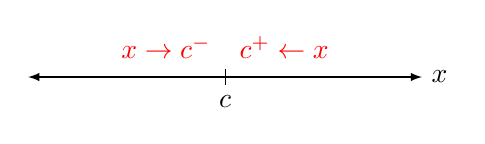
\begin{tikzpicture}
\draw[latex-latex] (-2.5,0) -- (2.5,0) node[right]{$x$} ; %edit here for the axis
%\draw [very thick, - latex, blue] (0,0) -- (2.5,0);
%\node[circle,draw=blue, fill=blue, inner sep=0pt,minimum size=5pt] (a) at (0,0) {};
\foreach \x in  {0} % edit here for the vertical lines
\draw[shift={(\x,0)},color=black] (0pt,3pt)  -- (0pt,-3pt);
\foreach \x in  {0}  % edit here for the numbers
\draw[shift={(\x,0)},color=black] (0pt,0pt) -- (0pt,-3pt) node[below] 
{$c$};
\foreach \x in  {-.75}  
\draw[shift={(\x,3pt)},color=red] node[above] {$x\to c^-$};
\foreach \x in  {.75}  
\draw[shift={(\x,3pt)},color=red] node[above] {$c^+\leftarrow x$};
\end{tikzpicture}
\caption{The notation $x\to c^-$ means that $x$ is approaching $c$ and $x<c$. The notation $x\to c^+$ means that $x$ is approaching  $c$ and $x>c$. }
\label{fig:leftrightlimit}
\end{figure}

\noindent
\fbox{\parbox{6in}{
The regular limit $\ds\lim_{x\to c}f(x)$ is sometimes called the ``two-sided" limit of $c$, and requires that $f(x)$ approaches one number for values of $x$ on both sides of $c$. This means that in order for $\ds\lim_{x\to c}f(x)$ to exist, the left and right limits at $c$ must exist and be equal:
\begin{quotation}
$\ds\lim_{x\to c}f(x)=L$  \qquad if and only if \qquad $\ds\lim_{x\to c^-}f(x) =L $ and $\ds\lim_{x\to c^+}f(x) =L $
\end{quotation}
}}

\begin{remark}
Remember that the phrase "if and only if" is shorthand for saying that one thing can only be true if the other is also true. In particular, if either right or left limit does not exist, or the left and right limits are equal to different numbers, then the two-sided limit does not exist. 
\end{remark}

\begin{example}
For example, the function $f$ graphed in \autoref{fig:TaalmanPage97-1} has a different limit from the left than from the right as $x$ approaches 1:

\begin{figure}[H]
\centering
\includegraphics[width=2in]{TaalmanPage97-1.png}
\caption{$\ds\lim_{x\to 1^-}f(x) = 2$ but $\ds\lim_{x\to 1^+} f(x) = 3$. So $\ds\lim_{x\to 1}f(x)\text{ DNE}$ even though $f(1)=3$. }
\label{fig:TaalmanPage97-1}
\end{figure}

The purple sequence of values of $x$ that approach $x=1$ from the left determines a sequence of values of $f(x)$ that approach $y=2$, while the red sequence determines values that approach $y=3$. The value of the function at $x=1$ happens to be $f(1)=3$, but that is not relevant to either limit calculation. Since the limits from the left and right are not the same, there is no one real number that the function approaches as $x\to c$ and we say the two-sided limit does not exist. 

In summary, there are {\bf three} limits associated to the point $x=1$ in the above picture:
$$\lim_{x\to 1^-} f(x) = 2,\quad \lim_{x\to 1^+} f(x) = 3, \quad \lim_{x\to 1} f(x) \text{ DNE}$$
\end{example}

\begin{exercise}
The function $g(x)$ is graphed below. Use the picture below to determine $\ds\lim_{x\to 1^-} g(x)$, $\ds\lim_{x\to 1^+} g(x)$, and $\ds\lim_{x\to 1} g(x)$. Are any of these equal to $g(1)$?
\begin{center}
\includegraphics[width=2.5in]{TaalmanPage99b.png}
\end{center}

\end{exercise}


%\todo{another example with VA of 1/x-1, pic from Taalman Page 97b}

\begin{example}
The function $f(x) = \frac{1}{x-1}$ is undefined at $x=1$ because the denominator $x-1$ is equal to zero. We can see in \autoref{fig:taalmanpage97b} that as $x$ approaches $1$ from the right, the values of the function increase without bound, so that
$$\lim_{x\to 1^+} f(x) = \infty.$$
As $x$ approaches $1$ from the left, the values of the function decrease without bound, so that
$$\lim_{x\to 1^-} f(x) = -\infty.$$
Since these the left and right limits do not agree with each other, we cannot make any nice statement about the two-sided behavior of the function at the point, and we write
$$\lim_{x\to 1} f(x) \text{ DNE}.$$

\begin{figure}[H]
\centering
\includegraphics[width=2.5in]{Images/TaalmanPage97b.png}
\caption{$\ds\lim_{x\to 1^-} f(x) = -\infty$ and $\ds\lim_{x\to 1^+} f(x) = \infty$. }
\label{fig:taalmanpage97b}
\end{figure}

\end{example}



%\todo{with one-sided limits: a real-world example and do the inst vel of the falling ball at $t=3$.}



\begin{example}[Application: A Real-World One-Sided Limit]
Let's return to our falling ball from Example \autoref{ex:fallingball}. Recall that the height of the ball at time $t$ (in seconds) is given in feet by the formula $s(t) = 64-16(t-1)^2$ and that the ball hits the ground at $t=3$. A graph of $s(t)$ for the domain of $0\leq t\leq 3$ is:

\begin{center}
\includegraphics[width=2.5in]{ACPrev1-1-1Graph.png}
\end{center}

How fast is the ball going when it hits the ground? In other words, what is the instantaneous velocity of the ball at $t=3$? Since this is the moment when our model ends, we can only consider values of $t$ that are less than $3$, and so we are interested in the limit 
$$\lim_{a\to 3^-} AV_{[a,3]}  = \lim_{a\to 3^-} \frac{s(3)-s(a)}{3-a}$$

Looking at a table of values for the average velocity on intervals getting smaller and smaller to the left of $t=3$:

\begin{table}[H]
\centering
\begin{tabular}{|l||c|c|c|c|c|c|c|}
\hline
Interval & $[2.5,3]$ & $[2.9,3]$ & $[2.99,3]$ & $[2.999,3]$ &  $[2.9999,3]$ & $[2.99999,3]$ &$t=3$ \\
\hline
Avg. Vel. (ft/sec) & $-56$ & $-62.4$ & $-63.84$ & $-63.984$ & $-63.9984$ & $-63.99984$ & $?$\\
\hline
\end{tabular}
\caption{Average velocities for $s(t) = 64-16(t-1)^2$ on intervals approaching $t=3$ from the left.}
\label{tab:instvelocityfallingball-landing}
\end{table}

Thus from this we infer that the limit is approaching $-63.999999\ldots  = -64$ and we write
$$\lim_{a\to 3^-} AV_{[a,3]}  = -64.$$

In context, we conclude that the ball is going 64 feet per second downward when it hits the ground. 


\end{example}

\subsection*{Summary}
The following terms were introduced in this section: 
\begin{quotation}
instantaneous velocity; limit of $f$ as $x$ approaches $c$ is equal to $L$, written $\ds\lim_{x\to c}f(x) = L$; DNE, meaning "does not exist"; limit of $f$ as $x$ approaches $c$  from the left is equal to $L$, written $\ds\lim_{x\to c^-}f(x) = L$; limit of $f$ as $x$ approaches $c$ from the right is equal to $L$, written $\ds\lim_{x\to c^+}f(x) = L$.
\end{quotation}

\textbf{Key ideas:} The limit of a function describes the behavior of the $y$-values of a function \textit{near} a point, rather than at a point. A limit does not exist if the $y$-values of a function do not approach a single number. We can take limits separately from the left (less than the input value) or the right (greater than the input value). 

\textbf{Other ideas introduced:} A limit only exists if both the right and left limits exist and are equal. Even though we can write that a limit is "equal to infinity," such a limit \textit{does not exist}. Instantaneous velocity is the (one- or two-sided) limit of average velocity. 




\begin{center}
\textcolor{ocre}{\fbox{\fbox{\Large \bf \sc End of Section 2.1}}}
\end{center}

\hspace{-.5in}\rule{1.1\textwidth}{2pt}








\section{Continuity}


\subsection*{Learning Goals}

\begin{itemize}
	\item What does it mean for a function to be continuous at a point, both visually and algebraically?
	\item What does it mean for a function to be continuous on an interval? On its domain?
	\item What does it mean for a function to be left or right continuous at a point?
	\item Be able to classify different types of discontinuity, visually and via limits. 
	\item See how continuous functions can be built from simpler functions so that "most" limits can be evaluated simply by plugging in. 
	\item Think about what limits we still cannot evaluate. 
\end{itemize}



\subsection{Definition of Continuity}
What do you think of when you hear the word "continuous?" A quick Google search will tell you that \textit{continuous} is an adjective that means
\begin{quotation}
\textit{forming an unbroken whole; without interruption.}
\end{quotation}
In this section, we define what it means for a function to be continuous, or to "have continuity."


\begin{example}\label{ex:continuity}
Consider the graph of the function $f(x) = \frac{1}{2}x+3$ below and the limit $\ds\lim_{x\to 2} f(x)$. 

\begin{figure}[H]
\centering
\includegraphics[width=2.5in]{altTaalmanPage125a.png}
\caption{The graph of $f(x) =  \frac{1}{2}x+3$. What is $\ds\lim_{x\to 2} f(x)$?}
\label{fig:taalmanpage125a}
\end{figure}

The limit asks us to consider what value the function $f(x)= \frac{1}{2}x+3$ approaches as $x$ approaches 2. We can see in the picture that the $y$-values of the function approach 4, and that this is also what we get when we evaluate the function at 2 since $f(2) = \frac{1}{2}(2)+3 = 1+3 = 4$. For this limit and this function, it is the case that 
$$\lim_{x\to 2}f(x) = f(2)=4$$
so that taking the limit is the same as evaluating the function. There is a particular name for this situation where the value of the limit is the same as the function's value: such a function is called \textbf{continuous}. 

\end{example}

Visually, a function is \textbf{continuous} if its graph has no breaks, jumps, or holes. Loosely speaking, you can sketch the graph of a continuous function "without picking up your pencil." 

\begin{example}[Non-examples]\label{ex:noncontinuity}
The three graphs in \autoref{fig:TaalmanPage125b-d} are not continuous at $x=1$. 

\begin{figure}[H]
	\centering
	\begin{subfigure}[H]{0.3\textwidth}
    		\centering
    		\includegraphics[width=0.8\textwidth]{TaalmanPage125b.png}
    		\caption{$y=g(x)$ is not continuous at $x=1$.}
    		\label{fig:TaalmanPage125b}
	\end{subfigure}
	\hspace{.2in}
	\begin{subfigure}[H]{0.3\textwidth}
		\centering
		\includegraphics[width=0.8\textwidth]{TaalmanPage125c.png}
		\caption{$y=h(x)$ is not continuous at $x=1$.}
		\label{fig:TaalmanPage125c}
	\end{subfigure}
	\hspace{.2in}
		\begin{subfigure}[H]{0.3\textwidth}
		\centering
		\includegraphics[width=0.8\textwidth]{TaalmanPage125d.png}
		\caption{$y=k(x)$ is not continuous at $x=1$.}
		\label{fig:TaalmanPage125d}
	\end{subfigure}
\caption{}
\label{fig:TaalmanPage125b-d}
\end{figure}

Visually, we notice the "gaps" in all three graphs at $x=1$. The left-most function $g(x)$ in \autoref{fig:TaalmanPage125b} has a "jump" at $x=1$. The left limit approaches 1 while the right limit approaches 2. The middle function $h(x)$ in \autoref{fig:TaalmanPage125c} and the right function $k(x)$ in \autoref{fig:TaalmanPage125d} have "holes" at $x=1$. All three graphs have "interruptions" at $x=1$, and so all three are not continuous at $x=1$. 



%all have some sort of ``special behavior" at $x=1$. The limits as $x\to 1$ detect exactly this special behavior: In each case, {\it the limit as $x\to 1$ is not the same as the value at $x=1$.}
%
%For example, in the left-most graph, $\ds\lim_{x\to 1}g(x)$ does not exist, but $g(1)=2$. 
%
%In the middle graph, $\ds\lim_{x\to 1}h(x)$ is equal to 1, while the value $h(1)$ is equal to 2. 
%
%Finally, in the right-most graph, $\ds\lim_{x\to 1}k(x)=1$ but the value of $k(1)$ does not exist. 
%
%Contrast all three of those behaviors with $\ds\lim_{x\to 1}f(x)=1$, which is equal to $f(1)=1$. You don't even notice the point on the graph; it's that boring.
\end{example}



The algebraic notation of limits makes the idea of continuity more precise. A function is continuous at a point $x=c$ if its limit as $x\to c$ is equal to a real number that is the same as the value of the function at $x=c$. 

\begin{definition}[Continuity of a Function]\label{def:continuous}
A function $f$ is \textbf{continuous at $x=c$} if $$\ds\lim_{x\to c}f(x) = f(c).$$
\end{definition}

\noindent
\fbox{\parbox{6in}{
The following three things need to be true about $f(x)$  in order for it to be continuous at $x=c$
\begin{itemize}
\item The function must be defined at $x=c$. In other words,  $x=c$ must be in the domain of $f$. 
\item The limit of $f(x)$ must exist at $x=c$. In other words, $\ds\lim_{x\to c}f(x)$ must be equal to a number. 
\item The limit of $f(x)$ at $x=c$ must be equal to the value of the function at $x=c$. 
\end{itemize}
}}

\begin{example}
In Example \ref{ex:continuity}, $f(x) = \frac{1}{2}x+3$ is continuous at $x=2$ because $\ds\lim_{x\to 2} f(x) = 4$ and $f(2)=4$, and these two things are equal. Note that $f(x)$ is continuous at every point pictured since at every point, the limit will equal the value of the function. 

\begin{figure}[H]
\centering
\includegraphics[width=2in]{altTaalmanPage125a.png}
\caption{The graph of $f(x) =  \frac{1}{2}x+3$ is continuous at all points pictured.}
\label{fig:taalmanpage125a-again}
\end{figure}

\end{example}

\begin{example}

By contrast, $g(x)$, $h(x)$, and $k(x)$ in Example \autoref{ex:noncontinuity} are not continuous at $x=1$ because the limits at $x=1$ are not equal to the values of the functions at $x=1$. 

%\todo{will need to break up into three subfigures pg 125 b-d}
%%\begin{center}
%%\includegraphics[width=4.5in]{TaalmanPage125b.png}
%%\end{center}



\begin{figure}[H]
	\centering
	\begin{subfigure}[H]{0.3\textwidth}
    		\centering
    		\includegraphics[width=0.8\textwidth]{TaalmanPage125b.png}
    		\caption{$\ds\lim_{x\to 1}g(x)$ DNE while \\$g(1)=2$.}
    		\label{fig:TaalmanPage125bagain}
	\end{subfigure}
	\hspace{.2in}
	\begin{subfigure}[H]{0.3\textwidth}
		\centering
		\includegraphics[width=0.8\textwidth]{TaalmanPage125c.png}
		\caption{$\ds\lim_{x\to 1}h(x)=1$  while $h(1)=2$.}
		\label{fig:TaalmanPage125cagain}
	\end{subfigure}
	\hspace{.2in}
		\begin{subfigure}[H]{0.3\textwidth}
		\centering
		\includegraphics[width=0.8\textwidth]{TaalmanPage125d.png}
		\caption{$\ds\lim_{x\to 1}k(x)=1$  while $k(1)$ is undefined.}
		\label{fig:TaalmanPage125dagain}
	\end{subfigure}
\caption{}
\label{fig:TaalmanPage125b-dagain}
\end{figure}

For $g(x)$, the limit does not exist and so cannot equal $g(1)=2$. For $h(x)$, the limit at $x=1$ is $1\neq h(1)=2$. For $k(x)$, the limit exists and is $\ds\lim_{x\to 1}k(x)=1$ while $k(1)$ is undefined, so cannot equal the limit. 

However, $g(x)$, $h(x)$, and $k(x)$ are continuous at every other $x$-value pictured. It is only at $x=1$ that these functions are not continuous. 

\end{example}

The functions that we will work with are almost always continuous, meaning that they are continuous at almost all points except for a few isolated points where they are discontinuous. Thus it makes sense for us to define what it means for a function to be continuous on an interval of points, rather than just point-by-point. 

\begin{definition}[Continuity of a Function on an Interval]
A function $f$ is \textbf{continuous on an interval} $(a,b)$ if it is continuous for every point $x=c$ with $a<c<b$. 

We say that a function is \textbf{continuous on its domain} if it is continuous on every interval on which it is defined. 
\end{definition}

\begin{example}
For instance, the function $h(x)$ from \autoref{fig:TaalmanPage125cagain} is continuous on the interval $(1,4)$ because it is continuous at all points $x=c$ with $1<c<4$. (Note the strict inequalities.) However, it is \textit{not} continuous on $(0,4)$ because it is not continuous at the point $x=1$ contained within the interval $(0,4)$. 

\begin{figure}[H]
\centering
		\includegraphics[width=1.5in]{TaalmanPage125c.png}
		\caption{$h(x)$ is continuous on $(1,4)$ but not on $(0,4)$.}
		\label{fig:TaalmanPage125cagain-again}
\end{figure}
\end{example}




\subsubsection{Left and Right Continuity}


\begin{example}\label{ex:rightcontinuityintro}
Note that in Example \ref{ex:noncontinuity}, the \textit{right} limit of $g(x)$ at $x=1$ is equal to the value of the function:
%$$\lim_{x\to 1^+} g(x) = 2 = g(1).$$

\begin{figure}[H]
\centering
		\includegraphics[width=1.5in]{TaalmanPage125b.png}
		\caption{The right limit $\ds\lim_{x\to 1^+}g(x) = 2$ is the same as $g(1) = 2$.}
		\label{fig:TaalmanPage125cagain-again}
\end{figure}

The {\it left} limit of $g(x)$, on the other hand, goes to 1, which is not the same as the value of the function at $x=1$:
$\ds\lim_{x\to 1^-} g(x) = 1\neq 2 = g(1).$
\end{example}

 Example \autoref{ex:rightcontinuityintro} above illustrates the need for yet another version of continuity that applies to only the left or right limit, instead of the two-sided limit. 

\begin{definition}[Left and Right Continuity at a Point]
A function $f$ is {\bf continuous from the left at $x=c$}, a.k.a. {\bf left-continuous}, if 
$$\lim_{x\to c^-}f(x) = f(c).$$


A function $f$ is {\bf  continuous from the right at $x=c$}, a.k.a {\bf right-continuous}, if 
$$\lim_{x\to c^+}f(x) = f(c).$$

\end{definition}

So the function $g(x)$ in Example \autoref{ex:rightcontinuityintro} above is  continuous from the right at $x=1$ but is not continuous from the left at $x=1$. 

We can use interval notation to express whether a function is right or left continuous at the edges of an interval. 

\begin{example}
The graphs that follow provide examples of continuity on the four possible types of bounded intervals. 

\begin{figure}[H]
\center
\includegraphics[width=6in]{TaalmanPage126.png}
\caption{Continuity on four different types of bounded intervals.}
\label{fig:taalmanpage126}
\end{figure}

For example, a function $f$ is continuous on $[1,3)$ if it is continuous at every point in the interior $(1,3)$ and continuous from the right at the left endpoint $x=1$, as shown in the second from left picture above. This is because the left endpoint is closed on the graph so that the left limit $\ds\lim_{x\to 1^+}f(x)$ at the left endpoint equals the value of the function $f(1)$. 

By contrast, the right-most picture above is continuous on $[1,3]$ since both endpoints are closed, so the right limit at $x=1$ matches $f(1)$, while the left limit at $x=3$ matches $f(3)$. This function is right-continuous at $x=1$ and left-continuous at $x=3$. 
\end{example}

\begin{example}\label{ex:jumpdisc}
Describe the continuity of the piecewise-defined function
$$g(x) = \begin{cases}
4-x^2, & \text{if }x\leq 1\\
x-1, & \text{if }x>1
\end{cases}$$
at the value $x=1$ by using the graph in  \autoref{fig:taalmanpage131b} below to determine the left, right, and two-sided limits at $x=1$. Then describe the intervals on which $g(x)$ is continuous. 

\begin{figure}[H]
\centering
\includegraphics[width=2in]{TaalmanPage131b.png}
\caption{Where is the function $g(x)$ continuous?}
\label{fig:taalmanpage131b}
\end{figure}
\end{example} 

\begin{solution}
We can see that 
$$\ds\lim_{x\to 1^-} g(x) = 3, \quad \ds\lim_{x\to 1^+}g(x) = 0,\quad \text{and}\quad g(1)=3.$$

$g(x)$ is  continuous from the left at $x=1$ because 
$$\ds\lim_{x\to 1^-} g(x) = 3=g(1).$$

$g(x)$ is not continuous from the right at $x=1$ because 
$$\ds\lim_{x\to 1^-} g(x) = 0\neq g(1)=3.$$ 

The two-sided limit $\ds\lim_{x\to 1}g(x)$ does not exist, and so $g(x)$ is not (both-sided) continuous at $x=1$. 

$g(x)$ is continuous at every other point, and so overall is continuous on the intervals
$$(-\infty, 1]\quad\text{and}\quad (1,\infty).$$
Remember that the closed endpoint on the interval $(-\infty,1]$ means that the function is continuous from the left at $x=1$. The open endpoint on the interval $(1,\infty)$ means that the function is not continuous from the right at $x=1$. 

\end{solution}


\begin{exercise}\label{ex:notdisc}
Follow the same process as in Example \autoref{ex:jumpdisc} to describe the continuity of the piecewise-defined function
$$f(x) = \begin{cases}
x+1, & \text{if }x< 1\\
3-x^2, & \text{if }x\geq1
\end{cases}$$
at the value $x=1$.  Use the graph in  \autoref{fig:taalmanpage131a} below to determine the left, right, and two-sided limits at $x=1$, and compare them to the value $f(1)$. Then describe the intervals on which $f(x)$ is continuous. 

\begin{figure}[H]
\centering
\includegraphics[width=2in]{TaalmanPage131a.png}
\caption{Where is the function $f(x)$ continuous?}
\label{fig:taalmanpage131a}
\end{figure}

\end{exercise}



\subsection{Types of Discontinuities}

When a function is not continuous at a point $x=c$, we say that it is {\bf discontinuous} at $x=c$. In terms of limits this means that 
\begin{quotation}
the limit $\ds\lim_{x\to c}f(x)$ is not equal to the value $f(c)$. 
\end{quotation}
The three  types of discontinuities that a function can have are illustrated as follows:

\begin{figure}[H]
\centering
\includegraphics[width=6in]{TaalmanPage126b.png}
\caption{The three types of discontinuities.}
\label{fig:taalmanpage126b}
\end{figure}

In the left-most picture, we see that the function is discontinuous at $x=2$ because $\ds\lim_{x\to 2}f(x) = 1$ while $f(2)=2$. This is called a \textbf{removable discontinuity}. Intuitively, we say that a discontinuity is removable if we could get rid of the discontinuity just by changing one value of the function. This type of discontinuity is also called a {\bf hole}.

In the middle picture, we can see that the function is discontinuous at $x=2$ because the left and right limits are different, so $\ds\lim_{x\to 2}f(x)$ does not exist. When the left and right limits both exist but are not equal, this is called a \textbf{jump discontinuity}. Here, $\ds\lim_{x\to 2^-} f(x) = 1$ and $\ds\lim_{x\to 2^+}f(x)  = 2$ both exist, but are not equal. At a jump discontinuity, the function jumps from one value to another. 

In the right-most picture, we see that the function is discontinuous at $x=2$ because $f(2)$ is undefined and the limit is not finite, and so does not exist. Anytime a left or right limit is infinite, we call this an \textbf{infinite discontinuity}. Infinite discontinuities are also called \textbf{vertical asymptotes}. 

To summarize, these types of discontinuities can be described precisely in terms of limits as follows:

\begin{definition}[Removable, Jump, and Infinite Discontinuities]
Suppose $f$ is discontinuous at $x=c$. We say that $x=c$ is a
\begin{enumerate}[label=\alph*.]
\item {\bf removable discontinuity} or {\bf hole} if $\ds\lim_{x\to c}f(x)$ exists but is not equal to $f(c)$, including the case where $f(c)$ is undefined. 
\item {\bf jump discontinuity} if $\ds\lim_{x\to c^-}f(x)$ and $\ds\lim_{x\to c^+} f(x)$ both exist and are finite but are not equal. It does not matter whether $f(c)$ is defined. 
\item {\bf infinite discontinuity} or {\bf vertical asymptote} if one or both of $\ds\lim_{x\to c^-} f(x)$ and $\ds\lim_{x\to c^+} f(x)$ is infinite. 
\end{enumerate}
\end{definition}

\begin{example}
What type of discontinuity does the function
$$g(x) = \begin{cases}
4-x^2, & \text{if }x\leq 1\\
x-1, & \text{if }x>1
\end{cases}$$
from Example \ref{ex:jumpdisc} have at $x=1$? 

\end{example}

\begin{solution}
Without looking at the picture, notice that as $x\to 1^-$, the piece of the function given by $4-x^2$ approaches $3$ algebraically:
$$\text{as }x\to 1^-,\quad 4-x^2\to 4-(1)^2 = 3.$$
Similarly, as $x\to 1^+$, the piece of the function given by $x-1$ approaches $0$ algebraically:
$$\text{as }x\to 1^+,\quad x-1\to 1-1 = 0.$$
Thus we can see algebraically that the function has a jump at $x=1$. We can confirm this by looking at the graph of $g(x)$:
\begin{figure}[H]
\centering
\includegraphics[width=2in]{TaalmanPage131b.png}
\caption{The function $g(x)$ has a jump discontinuity at $x=1$.}
\label{fig:taalmanpage131b-again}
\end{figure}
\end{solution}

\begin{exercise}
Is the function
$$f(x) = \begin{cases}
x+1, & \text{if }x< 1\\
3-x^2, & \text{if }x\geq1
\end{cases}$$
from Exercise \ref{ex:notdisc} discontinuous at $x=1$? If so, what type of discontinuity is it? Use the picture provided in \autoref{fig:taalmanpage131a} and then explain how you could see this algebraically from the formula for the function if you did not have a picture. 

Now consider the function 
$$h(x) = \begin{cases}
x+1, & \text{if }x< 1\\
3-x^2, & \text{if }x>1
\end{cases}$$
How is $h(x)$ different from $f(x)$? Is $h(x)$ discontinuous at $x=1$? If so, what type of discontinuity is it?
\end{exercise}


\subsection{Rules for Calculating Limits}
Now we know that limits of continuous function are easy to evaluate: we simply plug in the $x$-value of the limit to the formula, the same way we would if we just wanted to know the value of the function. In this section, we build up a list of functions that we know to be continuous. We begin with the simplest functions: constant and linear functions:



\begin{theorem}[Continuity of Linear Functions]\label{thm:contlinearfunctions}
Constant and linear functions are continuous for all $x$-values:
\begin{itemize}[]
\item For any real numbers $k$ and $c$, 
$$\lim_{x\to c}k = k$$%,\quad \lim_{x\to c}x = c,\quad \text{and}\quad\lim_{x\to c}(mx+b) = mc+b$$
\item For any real numbers $c, m,$ and $b$, 
$$\lim_{x\to c}(mx+b) = mc+b$$
\end{itemize}
\end{theorem}

Now we know that for any constant or any linear function, evaluating a limit is no different than evaluating the function. 

\begin{theorem}[Continuity of Power Functions]\label{thm:contpowerfunctions}

Power functions are continuous on their domains:
\begin{itemize}[]
\item For any real number $A$ and rational number $k$, then for any values $x=c$ for which $x^k$ is defined, 
$$\lim_{x\to c} Ax^k = Ac^k.$$
\end{itemize}
\end{theorem}

They key difference in Theorem \autoref{thm:contpowerfunctions} is that power functions are sometimes undefined, and so cannot be continuous where they are not defined, meaning outside of their domain. 


These are powerful theorems, because it tells us that we can calculate limits of certain simple functions at domain points just by evaluating the functions at those points. 

\begin{example}
For example, $f(x) = \frac{1}{x} = x^{-1}$ is a power function, so by Theorem \autoref{thm:contpowerfunctions}, it is continuous on its domain, which is $(-\infty,0)\cup(0\infty)$. This means that at any point $c\neq 0$ we can calculate $\ds\lim_{x\to c}\frac{1}{x}$ by simply calculating the value $f(c) = \frac{1}{c}$. 

For instance, 
$$\lim_{x\to 5}\frac{1}{x} = \frac{1}{5}$$
and 
$$\lim_{x\to -17}\frac{1}{x} = \frac{1}{-17}.$$

However, we \textit{cannot} yet compute $\ds\lim_{x\to 0}\frac{1}{x}$.  We will examine this limit in depth in a later section. 
\end{example}

\begin{example}
The function $f(x) = 2$ is constant. Hence using Theorem \autoref{thm:contlinearfunctions}, we know that
$$\lim_{x\to 3} 2 = 2.$$

The function $g(x) = x$ is linear, so again using Theorem \autoref{thm:contlinearfunctions}, we know that
$$\lim_{x\to 5} x = 5$$


The function $h(x) = \sqrt{x} = x^{1/2}$ is a power function, so using Theorem \autoref{thm:contpowerfunctions}, we know that
$$\lim_{x\to 16} \sqrt{x} = \lim_{x\to 16} x^{1/2} = (16)^{1/2} = \sqrt{16} = 4.$$

%We cannot yet compute 
%$$\lim_{x\to 4}\sqrt{x-1}$$
%but we will in a moment, and you can probably guess what it is equal to. 
\end{example}

%\begin{exercise}
%\todo{save this for later in the section}
%What do you think $$\lim_{x\to 4}\sqrt{x-1}$$ is equal to? 
%
%Note that this function isn't included in the previous theorem. It is an algebraic function, made up of the composition of the linear function $x-1$ inside the power function $\sqrt{x}$. 
%\end{exercise}


In Theorem \autoref{thm:contpowerfunctions}, the limit may sometimes be only one-sided. 

\begin{example}
For example, $f(x) = \sqrt{x} = x^{1/2}$ is defined at $x=0$ and for $x>0$, meaning to the right of $x=0$. However it is not defined for $x<0$, meaning to the left of $x=0$. Therefore the corresponding limit statement is one-sided:
$$\ds\lim_{x\to 0^+} \sqrt{x} = 0\quad \text{but}\quad \ds\lim_{x\to 0^-}\sqrt{x} \text{ DNE,}\quad\text{hence}\quad \lim_{x\to 0}\sqrt{x}\text{ DNE.}$$
\end{example}

\begin{exercise}
On what interval is $f(x) = \sqrt{x}$ continuous? {\it Hint: remember that $\sqrt{x}$ is a power function and Theorem \ref{thm:contpowerfunctions} says that power functions are continuous on their domains.}
\end{exercise}


\subsubsection{Limits of Combinations of Functions}
What about more complicated functions? Can we put together two continuous functions and still have a continuous function?

\begin{example}
For example, we already know from the continuity of power functions that
$$\lim_{x\to 2}x^2 = 2^2 = 4\quad\text{and}\quad\lim_{x\to 2}x^3 = 2^3 = 8.$$
Can we use these results to say something about
$$\lim_{x\to 2} (x^2+x^3)?$$
\end{example}

The key theorem that follows in Theorem \autoref{thm:limitrules} will help us answer this question; it says that limits can be evaluated within all of the arithmetic operations between function and even sometimes within a composition of functions. 

\newpage

\begin{theorem}[Rules for Calculating Limits of Combinations]\label{thm:limitrules}
If $\ds\lim_{x\to c} f(x)$ and $\ds\lim_{x\to c} g(x)$ exist and are finite, then the following rules hold for their combinations:

\begin{center}
\begin{tabular}{r l}
{\bf Constant Multiple Rule:} & $\ds\lim_{x\to c}k f(x) = k\lim_{x\to c} f(x)$ for any real number $k$\\
&\\
{\bf Sum Rule:} & $\ds\lim_{x\to c} (f(x)+g(x)) = \ds\lim_{x\to c}f(x) +\ds\lim_{x\to c}g(x)$\\
&\\
{\bf Difference Rule:} & $\ds\lim_{x\to c}(f(x)-g(x)) = \ds\lim_{x\to c}f(x)-\ds\lim_{x\to c}g(x)$\\
&\\
{\bf Product Rule:} &$\ds\lim_{x\to c}(f(x)\cdot g(x)) = \left(\ds\lim_{x\to c}f(x)\right)\cdot\left(\ds\lim_{x\to c}g(x)\right)$\\
&\\
{\bf Quotient Rule:} & $\ds\lim_{x\to c}\dfrac{f(x)}{g(x)} = \dfrac{\ds\lim_{x\to c}f(x)}{\ds\lim_{x\to c}g(x)}$, if $\ds\lim_{x\to c}g(x)\neq 0$ \\
&\\
{\bf Composition Rule:} & $\ds\lim_{x\to c}f(g(x)) = f\left(\ds\lim_{x\to c}g(x)\right)$, if $f$ is continuous at $\ds\lim_{x\to c}g(x)$. 
\end{tabular}
\end{center}

\end{theorem}

This theorem is a powerful tool for calculating limits, since it tells us how to find limits of compound functions in terms of the limits of their components. 

\begin{example}
For example, we can now calculate the limit of the \textbf{sum} $x^2+x^3$ as $x\to 2$ by taking the sum of the limits of $x^2$ and $x^3$ as $x\to 2$:
$$\lim_{x\to 2}(x^2+x^3) = \lim_{x\to 2}x^2+\lim_{x\to 2}x^3 = 2^2+2^3 = 4+8=12$$
\end{example}

\begin{example}
We can calculate $\ds\lim_{x\to 4}\sqrt{x-1}$ using the \textbf{Composition Rule}. For $f(x) = \sqrt{x}$ and $g(x) = x-1$, we have 
$$f(g(x)) = \sqrt{x-1}.$$ 
Since $\ds\lim_{x\to 4}x-1 = 3$ is in the domain of $f(x) = \sqrt{x}$, we know that $f(x)$ is continuous at $x=3$ and so
$$\lim_{x\to 4}\sqrt{x-1} = \sqrt{\lim_{x\to 4}(x-1)} = \sqrt{4-1} = \sqrt{3}$$
\end{example}


\begin{exercise}
Calculate the limits below using the continuity of linear and power functions and the limit rules in Theorem \ref{thm:limitrules}. Cite each part of Theorem \ref{thm:limitrules} that you apply. 

\begin{enumerate}[label=\alph*.,topsep=5pt,itemsep=10pt]
\item $\ds\lim_{x\to 3}(3x^2-2x+1)$
\item $\ds\lim_{x\to 1}(3x-1)^{12}$
\end{enumerate}
\end{exercise}


An immediate consequence of Theorem \ref{thm:limitrules} is that constant multiples, sums, differences, and products, quotients, and compositions of continuous functions are continuous:

\begin{theorem}[Combinations of Continuous Functions are Continuous]
Suppose that $f$ and $g$ are continuous at $x=c$ and $k$ is any constant. 
\begin{itemize}
\item The functions 
$$kf,\quad f+g,\quad f-g,\quad\text{and}\quad fg$$
are also continuous at $x=c$. \\

\item If $g(c)\neq 0$ then $\dfrac{f}{g}$ is continuous at $x=c$. \\

\item 
If $f$ is also continuous at $g(c)$, then $f\circ g$ is continuous at $x=c$. 
\end{itemize}
\end{theorem}


\begin{example}
For example, since $f(x)=x^2$ and $g(x) = x^3$ are continuous at $x=2$, we know that $(f+g)(x) = f(x)+g(x) = x^2+x^3$ must also be continuous at $x=2$. This makes sense given Theorem \ref{thm:limitrules} since
$$\lim_{x\to 2} (f+g)(x) = \lim_{x\to 2} (x^2+x^3) = \lim_{x\to 2} x^2+\lim_{x\to 2} x^3 = 2^2+2^3 = 4+8=12=(f+g)(2).$$
The key equality here is at either end: $\ds\lim_{x\to 2} (f+g)(x) = (f+g)(2)$. Remember, this is the definition of continuous from Definition \ref{def:continuous}.

\end{example}

What is the point of these rules and theorems? We now know that we can start with linear and power functions, and build up to any \textit{algebraic}\footnote{Recall that a function is \textit{algebraic} if it can be expressed with the use of only arithmetic operations ($+,-, \times, \div$) and rational  powers.} function via sums, differences, multiplication, division, or composition, and that the resulting function will be continuous as long as it is defined. In other words, as long as we stay within the domain of an algebraic function, we know that in order to evaluate the limit, we just plug it in. 


\begin{theorem}[Continuity of Algebraic Functions]\label{thm:contofalgebraicfunctions}
All algebraic functions are continuous on their domains. \\

\noindent
In particular, if $x=c$ is in the domain of an algebraic function $f$, then we can calculate $\ds\lim_{x\to c}f(x)$ by evaluating $f(c)$. 
\end{theorem}



With this theorem, we can evaluate any limit at a value where the expression is defined. Here are a few more examples:

\begin{example}
We can evaluate all of the following limits by simply plugging in:
\begin{enumerate}[label=\textbf{\alph*.},itemsep=10pt,topsep=5pt]
\item The expression $5\sqrt{x}+3$ is defined at $x=4$, so
$$\lim_{x\to 4}(5\sqrt{x}+3) = 5\sqrt{4}+3 = 5(2)+3 = 13$$


\item The expression $3x^4-7x$ is defined at $x=1$, so
$$\lim_{x\to 1} (3x^4-7x) = 3(1)^4-7(1) = -4$$


\item The expression $\dfrac{1+x}{3-x}$ is defined at $x=2$, so
$$\lim_{x\to 2}\frac{1+x}{3-x} = \frac{1+2}{3-2} = 3.$$
\end{enumerate}
\end{example}

\noindent
\textbf{Caution!} We have to be careful at the edge of a function's domain. The limits can only be one-sided. 

\begin{example}
For example, 
$$\lim_{x\to 2^+}\sqrt{x-2} = 0$$
since if $x\to 2^+$, this means $x>2$ and so $x$ is in the domain of $\sqrt{x-2}$. \\

\noindent
On the other hand, 
$$\lim_{x\to 2^-}\sqrt{x-2} \quad\text{ DNE}$$
since if $x\to 2^-$, this means $x<2$ and so $x$ is not in the domain of $\sqrt{x-2}$. We cannot take the limit on this side because the function is undefined, and so there is no sequence of $y$-values to analyze. 

Overall, 
$$\lim_{x\to 2}\sqrt{x-2} \quad\text{ DNE}$$
because the left and right limits do not both exist. Only the right limit exists and the function is continuous on
$$[2,\infty),$$
the same as its domain. 
\end{example}

\begin{exercise}
Calculate each of the following limits:
\begin{enumerate}[label=\alph*.,itemsep=10pt,topsep=5pt]
\item $\ds\lim_{x\to 0}\frac{2-x}{4-x^2}$
\item $\ds\lim_{x\to -3}\frac{2x^2+x-3}{x-1}$
\item $\ds\lim_{x\to 1}\frac{1}{\sqrt{x^3+3}}$
\end{enumerate}
%Which limits $x\to c$ do we not yet know enough to calculate for the above functions? In other words, what values $x=c$ are {\it not} in the domains of the expressions?
\end{exercise}


Note that Theorem \autoref{thm:contofalgebraicfunctions} does not tell us how to calculate limits at non-domain points. For example, we still do not know how to calculate $\ds\lim_{x\to 2}\frac{1}{x-2}$ (though maybe you have a guess). 

\begin{example}
We do not know how to calculate
$$\lim_{x\to -2} \frac{2-x}{4-x^2}\quad\text{or}\quad \lim_{x\to 2} \frac{2-x}{4-x^2}$$
since those $x$-values are not in the domain of $\frac{2-x}{4-x^2}$. \\

\noindent
Nor do we know how to calculate
$$\lim_{x\to 1}\frac{2x^2+x-3}{x-1}.$$

\noindent
Lastly, since $x^3+3\leq 0$ for $x\leq -\sqrt[3]{3}$, the expression $\frac{1}{\sqrt{x^3+3}}$ is undefined, so we do not know how to calculate
$$\lim_{x\to -\sqrt[3]{3}^+} \frac{1}{\sqrt{x^3+3}}.$$
Note that for $x< -\sqrt[3]{3}$, the expression $\frac{1}{\sqrt{x^3+3}}$ is undefined so any limit will simply fail to exist. 
\end{example}




\textbf{Key Take-away:} The only limits we have to "worry" about are at non-domain points of algebraic functions, and also the points of piecewise-defined functions where algebraic functions have been glued together and may or may not have jumps. 



%
%\begin{exercise}
%Determine whether each of the functions below is continuous, right-continuous, left-continuous, or discontinuous at $x=1$. Try to work algebraically first, and then check your answer by graphing the functions on Desmos. 
%\begin{enumerate}[label=\alph*., itemsep=10pt,topsep=5pt]
%\item $f(x) = \begin{cases}
%x+1, & \text{if }x<1\\
%3-x^2, & \text{if }x\geq 1
%\end{cases}$
%\item $g(x) = \begin{cases}
%4-x^2, &\text{if }x\leq 1\\
%x-1, &\text{if }x>1
%\end{cases}$
%\end{enumerate}
%\end{exercise}


\subsection*{Summary}
The following terms were introduced in this section: 
\begin{quotation}
continuous and continuity of functions at a point and on an interval; continuous from the right and continuous from the left; discontinuous and discontinuity; removable discontinuity a.k.a. hole; jump discontinuity; infinite discontinuity a.k.a vertical asymptote
\end{quotation}

\textbf{Key ideas:} A function is continuous if the value of a limit is the same as the value of the function. This means the graph has no breaks. At a point of discontinuity, you can either have a hole, jump, or vertical asymptote. Algebraic functions are continuous on their domains. 

\textbf{Other ideas introduced:} We need other methods to evaluate limits at non-domain points. 




\begin{center}
\textcolor{ocre}{\fbox{\fbox{\Large \bf \sc End of Section 2.2}}}
\end{center}

\hspace{-.5in}\rule{1.1\textwidth}{2pt}







\section{The Intermediate Value Theorem}


\subsection*{Learning Goals}

\begin{itemize}
	\item Understand the statement of the Intermediate Value Theorem:
	\begin{itemize}
		\item Represent the variables and notation in the Theorem visually.
		\item Identify the hypotheses of the theorem and why they are necessary. 
		\item Identify the conclusion of the theorem and the ways in which it may fail if the hypotheses are not true. 
	\end{itemize}
	\item Understand how the IVT implies that a function can change sign only at zeros and discontinuities. 
	\item Determine where a piecewise-defined function is positive and negative. 
\end{itemize}


\subsection{Motivational Scenario}

I'm melting sugar into caramel while watching the latest episode of The Great British Baking Show on Netflix. It's taking forever for my stove to come up to temperature and I need to be careful: sugar caramelizes at 340 degrees Fahrenheit (170 degrees Celsius) and will quickly start to burn if it gets too hot. 

I'm momentarily transfixed by Abdul's stunning parrot mask biscuit showstopper. Oh no! My sugar has overheated and burned. I'm so annoyed with myself. If I had paid more attention, I could have caught the moment it reached the right temperature and prevented this disaster.  

There are several (mathematical) assumptions that feed into my frustration. 
\begin{enumerate}
\item The temperature of the sugar could not have jumped over $340^\circ$F. 
\item There is a point in time at which the temperature was exactly $340^\circ$F. 
\item That time must have been while I was distracted because the sugar went from too cool to too hot when I wasn't looking.
\end{enumerate}

All of these assumptions (and my resulting frustration) are encapsulated by the Intermediate Value Theorem, which states that continuous functions, such as temperature, cannot skip values, such as $340^\circ$F.


\subsection{The Intermediate Value Theorem}
In this section, we examine an important consequence of continuity that extends beyond our desire to describe a single value of a function. If $f$ is continuous between two values $x=a$ and $x=b$, then the corresponding values of $f(x)$ go through every possible intermediate value between the $y$-values $f(a)$ and $f(b)$. This is intuitively obvious if we think of continuous functions as having ``unbroken" graphs. 

For example, consider the function $f$ in the figure that follows. The function is equal to every {\t intermediate} value $y=K$ between $y=f(a)$ and $y=f(b)$:

\begin{figure}[H]
\centering
\includegraphics[width=2in]{TaalmanPage129c.png}
\caption{The continuous function $f(x)$ has height $y=K$ at $x=c$.}
\label{fig:taalmanpage129c}
\end{figure}

In general, passing through all  such "intermediate values" is a property that holds for every function that is continuous on a closed interval $[a,b]$:

\begin{theorem}[The Intermediate Value Theorem]
Suppose that $f$ is a continuous function on a closed interval $[a,b]$ such that $f(a)\neq f(b)$ and $K$ is any $y$-value strictly between $y=f(a)$ and $y=f(b)$. 
Then there exists at least one $x$-value $c$ between $x=a$ and $x=b$ such that $f(c)=K$. 
\end{theorem}

This important consequence of continuity may seem obvious, but in fact it relies on a subtle mathematical property of the real numbers called the {\it Least Upper Bound Axiom.} Properly explaining why the Intermediate Value Theorem is true is outside of the scope of this book.

In the Intermediate Value Theorem, the hypothesis that $f$ be continuous on a closed interval is essential. If $f$ either fails to be continuous on the interior of the interval or fails to be continuous at a closed endpoint, then the conclusion of this theorem does not necessarily hold. For example, the function below fails to be continuous on $[a,b]$ and also fails to satisfy the conclusion of the Intermediate Value Theorem for the pictured value of $K$. 

Note that this theorem has two different parts: 
\begin{itemize}
\item The \textbf{hypothesis} of the theorem are the conditions that need to be met in order to apply the theorem. 
\item The \textbf{conclusion} of the theorem is what the theorem tells us to be true, given that the conditions in the hypothesis are met.
\end{itemize}
The \textbf{hypotheses} of the Intermediate Value Theorem are
\begin{itemize}[topsep=10pt,leftmargin=1.5in]
\item $f$ must be continuous on the closed interval $[a,b]$, 
\item $f(a)\neq f(b)$, and
\item $K$ must be a $y$-value strictly between $f(a)$ and $f(b)$.
\end{itemize}

\noindent
The \textbf{conclusion} of the Intermediate Value Theorem is
\begin{itemize}[topsep=10pt,leftmargin=1.5in]
\item that there is at least one value $x=c$ that is between $x=a$ and $x=b$ such that $f(c)=K$, meaning that the function $f$ has height $y=K$ \textit{somewhere} on the interval from $x=a$ to $x=b$. 
\end{itemize}



\begin{example}\label{ex:IVTintroex}
We can use the Intermediate Value Theorem to show that
$$x^4+x=3$$
has a solution for some $x$-value between $x=1$ and $x=2$. 

First, define the function $f(x) = x^4+x$. We are given $x$-values $x=1$ and $x=2$, so in the IVT, we are using $a=1$ and $b=2$. We want to know that $f(x) = 3$, so in the IVT we are using $K=3$. 

Let's check that the hypotheses of the IVT are true:
\begin{itemize}
\item $f$ is algebraic with domain $\mathbb{R}$, hence $f$ is continuous on $[1,2]$. 
 \item $f(1) = (1)^4+1 = 2$ and $f(2) = (2)^4+2 = 18$, so $f(1)\neq f(2)$. 
 \item $K=3$ is strictly between $f(1) = 2$ and $f(2) = 18$. 
\end{itemize}
Since the hypotheses are all met, we may use the conclusion:
\begin{itemize}
 \item There is a value of $x=c$ between $x=1$ and $x=2$ such that
 $$\begin{aligned}
 f(c) &= 3\\
 c^4+c &= 3
\end{aligned}$$
\end{itemize}
Thus we know that $x=c$ is a solution to the equation $x^4+x=3$ and that $1<c<2$. 

Do we know the precise value of $c$? No, we do not. We can \textit{guess} that $x=c$ is fairly close to $x=1$, since $f(1)=2$ is close to $K=3$ (especially compared to $f(2) = 18$), but we don't know that for a fact. It's also possible that there is more than one solution to the equation $x^4+x=3$ between $x=1$ and $x=2$. The IVT does not specify how many values of $c$ there are, just that at least one exists. 

\end{example}

\begin{exercise}
Use Desmos to graph $f(x) = x^4+x$ and $y=3$. How many values of $x=c$ are there with $f(c) = 3$ and $1<c<2$? Estimate them from the graph. 
\end{exercise}


As noted in Example \autoref{ex:IVTintroex}, there may be more than one value of $c$ which satisfies the conclusion of the IVT:

\begin{figure}[h]
	\centering
	\begin{subfigure}[H]{0.4\textwidth}
    		\centering
    		\includegraphics[width=\textwidth]{IVTPic1.png}
    		\caption{There may be only one $x=c$ with $f(c) = K$ (pictured here $f(c)=N$).}
    		\label{fig:IVTPic1}
	\end{subfigure}
	\hspace{.2in}
	\begin{subfigure}[H]{0.4\textwidth}
		\centering
		\includegraphics[width=\textwidth]{IVTPic2.png}
		\caption{There may be more than one $x=c$ with $f(c) = K$ (pictured here $f(c)=N$).}
		\label{fig:IVTPic2}
	\end{subfigure}
	\caption{There is \textit{at least} one $x=c$ with $f(c) = K$ (pictured here $f(c) = N$). }
	\label{fig:IVTPics}
\end{figure}



\begin{example}[A real-world illustration of the Intermediate Value Theorem]
Consider the function $w(t)$ that describes a particular person's weight at $t$ years of age between the ages of 18 and 45. 

The weight function $w(t)$ should be continuous on $[18,45]$ because a person's weight changes continuously over time and cannot jump from one value to another. (We are assuming typical circumstances, so that a person does not get a serious haircut, lose a limb, or somehow otherwise get their weight to change drastically in an instant.)

The Intermediate Value Theorem tells us that for every weight $K$ between $w(18)$ and $w(45)$, there is some time $c$ between 18 and 45 for which $w(c) = K$. For example, if the person weighed $w(18)=130$ pounds at age 18 and $w(45)=163$ pounds at age 45, then there must be some age between 18 and 45 at which the person weighed, say, exactly 144 pounds. In fact, we know that the person must have weighed all of the weights between 130 and 163 pounds, at least once between ages 18 and 45. 

It's also entirely possible that the person may have weighed exactly 144 pounds multiple times between ages 18 and 45, and we don't know exactly when the person weighed exactly 144 pounds from the theorem. 
\end{example}


\begin{example}[Applying the Intermediate Value Theorem]\label{ex:applyingIVT}
The function $f(x) = x^3-3x+1$ is continuous everywhere as we saw in Theorem \ref{thm:contofalgebraicfunctions}. We use the Intermediate Value Theorem to conclude that there is some point $c$ for which $f(c)=2$, even though we cannot solve the equation $x^3-3x+1=2$ by hand. 

To show that there is some $c$ with $f(c)=2$, we need to find values $a$ and $b$ such that $K=2$ is between $y=f(a)$ and $y=f(b)$, and apply the Intermediate Value Theorem. By trial and error, we can find such values $a$ and $b$, by testing different value of $f(x)$ until we find one that is less than and one that is greater than $2$. For example, 
$$\begin{aligned}
f(0)&=0^3-3(0)+1 = 1<2,\\
f(2)&=2^3-3(2)+1 = 3>2.
\end{aligned}$$
Since $f$ is continuous on $[0,2]$ and $K=2$ satisfies $f(0)<K<f(2)$, by the Intermediate Value Theorem there is some value $c$ between $x=0$ and $x=2$ for which $f(c)=2$. Note that the Intermediate Value Theorem doesn't tell us where $c$ is, only that such a $c$ exists somewhere in the interval $(0,2)$. 

\end{example}

\begin{exercise}
Use Desmos to graph $f(x) = x^3-3x+1$ and $y=2$. Click on the point of intersection that is between the $x$-values $x=0$ and $x=2$ and estimate the value of $c$ predicted by the IVT in Example \ref{ex:applyingIVT}. There are other values of $c$ that also satisfy $f(c)=2$, but they are not on the interval where we used the Theorem. 
\end{exercise}


\subsection{Why All of the Hypotheses of the IVT are Necessary}

The conclusion of the Intermediate Value Theorem may fail if any one of the hypotheses of the theorem is not satisfied. 


\begin{description}
\item[Continuous on an interval] Suppose that $f(x)$ is discontinuous somewhere on the interval $[a,b]$. Such a graph may look like the one in \autoref{fig:taalmanpage129e}.

\begin{figure}[H]
\centering
\includegraphics[width=2in]{TaalmanPage129e.png}
\caption{A discontinuous function may miss a $y$-value $K$ between $f(a)$ and $f(b)$.}
\label{fig:taalmanpage129e}
\end{figure}

We can see from the graph that a function that is not continuous on $[a,b]$ may miss a $y$-value between $f(a)$ and $f(b)$. 

\item[The interval is closed] Suppose that $f(x)$ is discontinuous at one of the endpoints of the interval $[a,b]$. Such a graph may look like the one in \autoref{fig:taalmanpage129d-mod}. 


\begin{figure}[H]
\centering
\includegraphics[width=2in]{TaalmanPage129d-mod.png}
\caption{A function continuous on $[a,b)$ may miss a $y$-value $K$ between $f(a)$ and $f(b)$.}
\label{fig:taalmanpage129d-mod}
\end{figure}

We can see from the graph that a function that is not continuous at one of the endpoints, for example at $x=b$, may miss a $y$-value between $f(a)$ and $f(b)$. 


\item[$K$ is between $f(a)$ and $f(b)$] If $K$ is not between the $y$-values $f(a)$ and $f(b)$, then that value may be outside the range of $y$-values that the function has, as displayed in \autoref{fig:taalmanpage129a-mod} below. 

\begin{figure}[H]
\centering
\includegraphics[width=2in]{TaalmanPage129a-mod.png}
\caption{A function may miss a $y$-value $K$ that is not between $f(a)$ and $f(b)$.}
\label{fig:taalmanpage129a-mod}
\end{figure}


\item[$\mathbf{f(a)\neq f(b)}$] If $f(a)=f(b)$, then there are no $y$-values $K$ that are strictly between $f(a)$ and $f(b)$. In other words, there are no "intermediate" values to consider. 

\end{description}


\subsection{Where a Function Can Change Sign}
Dear reader, you have been using the Intermediate Value Theorem for some time now without knowing it! An extremely useful special case of the Intermediate Value Theorem is the case when we consider the intermediate value $K=0$. In this case, the Intermediate Value Theorem says that if $f$ is continuous on $[a,b]$ and $f(a)$ and $f(b)$ have opposite signs (one positive, one negative), then there exists at least one $x=c$ between $x=a$ and $x=b$ where $f(c)=0$, meaning that $x=c$ is a zero of $f(x)$. 

Said another way: if a function is going to switch from positive to negative or vice versa, it either has to pass through the $x$-axis somewhere (where $y=0$), or else it has to jump over it somehow, meaning it is discontinuous. The IVT forces the function to cross the $x$-axis at a specific value $x=c$ in order to change signs, unless the function is discontinuous, in which case the IVT does not apply. 

We use this special application of the IVT every time we solve an inequality by checking signs between zeros and discontinuities!

\begin{theorem}[A Function Can Change Sign Only at Zeros and Discontinuities]\label{thm:changesign}
A function $f$ can change sign (from positive to negative or vice versa) at a point $x=c$ only if $f(x)$ is zero, undefined, or discontinuous at $x=c$. 
\end{theorem}

The graph in \autoref{fig:taalmanpage130a} at the left shows a function $f$ that is continuous on $[a,b]$, and changes sign only at its zeros $c_1, c_2$, and $c_3$. The graph in \autoref{fig:taalmanpage130b} at the right is discontinuous somewhere in $[a,b]$ and therefore can change sign as we move from left to right without ever crossing the $y$-axis. 



\begin{figure}[h]
	\centering
	\begin{subfigure}[H]{0.4\textwidth}
    		\centering
    		\includegraphics[width=\textwidth]{TaalmanPage130a.png}
    		\caption{$f(x)$ can change sign at zeros.}
    		\label{fig:taalmanpage130a}
	\end{subfigure}
	\hspace{.2in}
	\begin{subfigure}[H]{0.4\textwidth}
		\centering
		\includegraphics[width=\textwidth]{TaalmanPage130b.png}
		\caption{$f(x)$ can change sign at a discontinuity.}
		\label{fig:taalmanpage130b}
	\end{subfigure}
	\caption{A function can change sign only at zeros and discontinuities. }
	\label{fig:taalmanpage130}
\end{figure}



%\todo{replace pic and put in figure}
%\begin{center}
%\includegraphics[width=5in]{TaalmanPage130.png}
%\end{center}

\begin{exercise}
Explain in your own words why a function $f$ can change sign at $x=c$ only if $f(x)$ is zero, undefined, or discontinuous at $x=c$. (Imagine that you are explaining this to one of your classmates while working at the board during class.)
\end{exercise}


\begin{example}
Determine the intervals on which the function 
$$f(x) = \begin{cases}
x+1,& \text{if } x<-2\\
(x+1)^2,& \text{if } -2\leq x\leq 1\\
2-x,& \text{if } x>1
\end{cases}$$
is positive and negative. 
\end{example}

\begin{solution}
The piecewise-defined function $f$ can be discontinuous only at its break points $x=-2$ and $x=1$. We check whether the left and right limits at each point are the same. 

\begin{itemize}
\item At $x=-2$, we use the piece $x+1$ to the left and the piece $(x+1)^2$ to the right:
$$\begin{aligned}
\lim_{x\to -2^-}f(x) &= \lim_{x\to -2^-}x+1 = -2+1 = -1\\
\lim_{x\to -2^+}f(x) &=\lim_{x\to -2^+}(x+1)^2 = (-2+1)^2 = (-1)^2 = 1
\end{aligned}$$
The left and right limits are different, so the function is discontinuous at $x=-2$; it has a jump. 


\item At $x=1$ we use the piece $(x+1)^2$ to the left and the piece $2-x$ to the right:
$$\begin{aligned}
\lim_{x\to 1^-}f(x) &= \lim_{x\to 1^-}(x+1)^2 = (1+1)^2 = (2)^2 = 4\\
\lim_{x\to 1^+}f(x) &=\lim_{x\to 1^+}2-x = 2-1 = 1
\end{aligned}$$
The left and right limits are different, so the function is discontinuous at $x=1$; this is also a jump. 
\end{itemize}
Thus $f(x)$ is discontinuous at $x=-2,1$. \\

\noindent
Next, let's check whether $f(x)$ is ever equal to zero. We must look at each piece of the function separately, and remember what $x$-values we use for each piece. 

\begin{itemize}
\item Its first piece, $x+1$ is equal to zero when $x=-1$, which is not on the interval $x<-2$ where that piece is used. So that part of the function is never equal to zero. 

\item The second piece $(x+1)^2$ is zero  at $x=-1$. That is within the interval $-2\leq x\leq 1$ on which the piece is used, so the function is equal to zero at $x=-1$. 

\item The third piece $2-x$ is zero when $x=2$. That is on the interval $x>1$ where that piece is used, so the function is also equal to zero at $x=2$. 
\end{itemize}
Thus $f(x)$ is equal to zero at $x=-1, 2$. \\


\noindent
By Theorem \ref{thm:changesign} the function $f$ can change sign only at the zeros, $x=-1, 2$, and discontinuities, $x=-2,1$. We put these points on a number line, marking 0 for zeros and {\sc DC} for discontinuities, then check the sign of $f$ one time between each of these points: 


%%%%%%%%%%%%%%
%%%%%%%%Number line
%%%%%%%%%%%%%%
\begin{center}
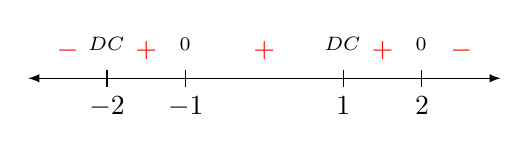
\begin{tikzpicture}
\draw[latex-latex] (-3,0) -- (3,0) ; %edit here for the axis
%\draw [very thick, - latex, blue] (0,0) -- (2.5,0);
%\node[circle,draw=blue, fill=blue, inner sep=0pt,minimum size=5pt] (a) at (0,0) {};
\foreach \x in  {-2,-1,1,2} % edit here for the vertical lines
\draw[shift={(\x,0)},color=black] (0pt,3pt) -- (0pt,-3pt);
\foreach \x in  {-2,-1,1,2}  % edit here for the numbers
\draw[shift={(\x,0)},color=black] (0pt,0pt) -- (0pt,-3pt) node[below] 
{$\x$};
\foreach \x in  {-1,2}  % edit here for 0's
\draw[shift={(\x,3pt)}] node[above] {$^0$};
\foreach \x in  {-2,1}  % edit here for DC's
\draw[shift={(\x,3pt)}] node[above] {$^\text{DC}$};
\foreach \x in  {-1.5,0,1.5}  % edit here for +'s
\draw[shift={(\x,3pt)},color=red] node[above] {$+$};
\foreach \x in  {-2.5,2.5}  % edit here for -'s
\draw[shift={(\x,3pt)},color=red] node[above] {$-$};
\end{tikzpicture}
\end{center}

\noindent
Lastly, recall that $f(x)$ is defined at each of the discontinuities. $f(-2) = 1$ and $f(1) = 4$, so $f(x)$ is positive at both of these endpoints. Remember that $0$ is neither positive nor negative. Thus reading from the signs on the number line, we see that $f(x)$ is positive between $-2$ and $-1$, including at $-2$, and also between $-1$ and $2$, where at $x=1$ the function remains positive. 


\begin{center}
\fbox{
$f(x)$ is negative on $(-\infty,-2)\cup(2,\infty)$ and positive on $[-2,-1)\cup(-1,2)$. 
}
\end{center}

\end{solution}







\subsection*{Summary}
The following terms and theorems were introduced in this section: 
\begin{quotation}
the Intermediate Value Theorem, hypothesis, conclusion.
\end{quotation}

\textbf{Key ideas:} The hypotheses of a theorem must be true in order to apply the conclusion of the theorem, so we must always check the hypotheses before using a theorem. The Intermediate Value Theorem tells us that a continuous function on a closed interval must be equal to all of its intermediate $y$-values at some point (or multiple points). Because of the  IVT, a function can only change sign at zeros or discontinuities. 

\textbf{Other ideas introduced:} We can apply the IVT to find intervals of $x$-values on which a continuous function must be equal to a particular value $y=K$, provided that we know the function is equal to values that are larger and smaller than $K$. 




\begin{center}
\textcolor{ocre}{\fbox{\fbox{\Large \bf \sc End of Section 2.3}}}
\end{center}

\hspace{-.5in}\rule{1.1\textwidth}{2pt}








\section{Infinite Limits and Limits at Infinity}


\subsection*{Learning Goals}

\begin{itemize}
	\item What does it mean mathematically to have an infinite limit, or to take a limit at infinity?
	\item Learn the definitions of vertical and horizontal asymptotes and be able to identify them visually. 
	\item Use limit notation to describe vertical and horizontal asymptotes.
	\item Learn about limits of the form $\frac{1}{0}$
	\item Use sign analyses to determine whether infinite limits approach positive or negative infinity
\end{itemize}



\subsection{Definitions: Infinite Limits and Limits at Infinity}

The wonderful thing about continuity is that it lets us calculate limits by evaluation. But what are we supposed to do with the limits that we cannot just evaluate, such as at $x$-values that are not in the domain of a function? We begin to investigate with a simple example:

%\todo{Quick example with $f(x) = \frac{1}{x}$ at $x=0$. }

\begin{example}\label{ex:VAmotivation}
For example, the function $f(x) = \frac{1}{x}$ is undefined when $x=0$, so the only limit of this function that we cannot calculate by simply plugging in is
$$\lim_{x\to 0}\frac{1}{x}.$$

The graph of $f(x) = \frac{1}{x}$ is in \autoref{fig:taalmanpage52binfinitelimit} below:

\begin{figure}[H]
\centering
\includegraphics[width=2in]{TaalmanPage52b.png}
\caption{$f(x) = \frac{1}{x}$ is undefined at $x=0$.}
\label{fig:taalmanpage52binfinitelimit}
\end{figure}

Based on \autoref{fig:taalmanpage52binfinitelimit}, you may be able to see what $\ds\lim_{x\to0}\frac{1}{x}$ should be. In case it isn't clear to you, here is a table of values for $f(x) = \frac{1}{x}$ as $x\to 0$ from both the left and right. 

\begin{table}[H]
\centering
\begin{tabular}{|c||c|c|c|c|c|c|c|c|c|c|c|}
\hline
$x$ & $-1$ & $-0.5$ & $-0.1$ & $-0.01$ & $-0.001$ & \textbf{0} & 0.001 & 0.01 & 0.1 & 0.5 & 1\\
\hline
$1/x$ & $-1$ & $-2$ & $-10$ & $-100$ & $-1000$ & \textbf{?} & 1000 & 100 & 10 &2 & 1\\
\hline
\end{tabular}
\caption{A table of values for $f(x) = \frac{1}{x}$ as $x\to 0$.}
\label{tab:vaofoneoverx}
\end{table}

We can see that as $x\to 0^+$, the values of $\frac{1}{x}$ become larger and larger. We write this using limit notation as
$$\lim_{x\to 0^+}\frac{1}{x} = \infty.$$
Similarly, we can see that as $x\to 0^-$, the values of $\frac{1}{x}$ become larger and larger, and are negative. We write this using limit notation as
$$\lim_{x\to0^-}\frac{1}{x} = -\infty.$$
Since the right and left limits do not agree, we cannot make any two-sided limit statement, other than to say that
$$\lim_{x\to 0}\frac{1}{x}\text{ DNE, because the right and left limits are not equal.}$$
This last answer is not particularly informative or useful, and so our REAL answer for the limit as $x\to 0$ is to describe both the left and right limits as precisely as we can: 
$$\boxed{\lim_{x\to 0^+}\frac{1}{x} = \infty\quad\text{and}\quad \lim_{x\to0^-}\frac{1}{x} = -\infty.}$$
\end{example}

%\todo{Definition of infinite limit. What I have here? Compare with Taalman and APC. Not sure what's easiest to understand}

Example \autoref{ex:VAmotivation} demonstrates the necessity of defining a notation that describes the values of a function becoming infinitely large, either positively or negatively. This is stated more carefully in Definition \autoref{def:infinitelimit} below: 

\begin{definition}[Definition of Infinite Limits]\label{def:infinitelimit}
Given a function $f$ and a fixed input $x=c$, we say that {\bf $f$ approaches infinity as $x$ approaches $c$} and write
$$\lim_{x\to c}f(x) = \infty$$
provided that we can make the values of $f(x)$ as large as we like by taking $x$ sufficiently close (but not equal) to $c$. 


Similarly, we say that {\bf $f$ approaches negative infinity as $x$ approaches $c$} and write
$$\lim_{x\to c}f(x) = -\infty$$
provided that we can make the values of $f(x)$ as large and negative as we like by taking $x$ sufficiently close (but not equal) to $c$. 

Either of these statements can be modified appropriately for left and right limits. 
\end{definition}

%\todo{remark about limits existing or not}

\noindent
\fbox{
\parbox{6in}{
Recall that in Definition \autoref{def:limit}, a limit does not exist if there is no single value that $f(x)$ approaches as $x\to c$. That is the case for \textit{every} infinite limit: there is no finite value that the function approaches. Even though we write that the limit is "equal to" $\infty$ or $-\infty$, these limits \textit{do not exist} because $\infty$ and $-\infty$ are not real numbers. 
}}

\begin{example}\label{ex:moreVAmotivation}
We can see from the graph of $g(x) = \frac{1}{x^2}$ in \autoref{fig:taalmanpage301b-1verticalasymptote} that
$$\lim_{x\to 0^-}\frac{1}{x^2} = \infty\quad\text{and}\quad \lim_{x\to 0^+}\frac{1}{x^2} = \infty$$
so that
$$\lim_{x\to 0}\frac{1}{x^2} = \infty.$$
This means only that the values of $\frac{1}{x^2}$ become infinitely large as $x\to 0$. The limit still does not \textit{exist}. However, we do NOT write $\lim_{x\to 0}\frac{1}{x^2}$ DNE because that does not give us any useful information. Remember: limits are used to describe the behavior of functions, not simply spit out an answer, so we want our answers to be as descriptive as possible. 

\begin{figure}[H]
\centering
\includegraphics[width=1.5in]{TaalmanPage301b-1.png}
\caption{$\ds\lim_{x\to 0}\frac{1}{x^2} = \infty$.}
\label{fig:taalmanpage301b-1verticalasymptote}
\end{figure}


\end{example}


\begin{exercise}
In your own words, explain what it means for a limit to be "equal to infinity."
\end{exercise}

The graphs of $f(x) = \frac{1}{x}$ and $g(x) = \frac{1}{x^2}$ motivate another type of limit. Notice that the $y$-values of both functions approach the $x$-axis at the far left and right ends of the graph. There appears to be a particular "long-term" behavior for both functions that is worth describing. 

%\todo{Quick example with $f(x) = \frac{1}{x}$ as $x\to\pm\infty$}


\begin{example}
If instead of looking at the middle of the graphs, we look at the \textit{ends}, we can see that as $x$ becomes very large, either positively or negatively, the values of both $f(x) = \frac{1}{x}$ and $g(x) = \frac{1}{x^2}$ become smaller and smaller. 

\begin{figure}[H]
	\centering
	\begin{subfigure}[H]{0.3\textwidth}
    		\centering
    		\includegraphics[width=0.8\textwidth]{TaalmanPage150c.png}
    		\caption{$\ds\lim_{x\to\infty}\frac{1}{x} = 0$.}
    		\label{fig:TaalmanPage150c}
	\end{subfigure}
	\hspace{.2in}
	\begin{subfigure}[H]{0.3\textwidth}
		\centering
		\includegraphics[width=0.8\textwidth]{TaalmanPage150d.png}
		\caption{$\ds\lim_{x\to\infty}\frac{1}{x^2} = 0$.}
		\label{fig:TaalmanPage150c}
	\end{subfigure}
	\caption{$f(x) = \frac{1}{x}$ and $g(x) = \frac{1}{x^2}$ have finite limits as $x\to\infty$. }
	\label{fig:taalmanpage150cd}
%\centering
%\includegraphics[width=1.5in]{TaalmanPage150c.png}
%\includegraphics[width=1.5in]{TaalmanPage150d.png}
%\caption{As $x$ becomes very large, the values of $f(x) = \frac{1}{x}$ and $g(x) = \frac{1}{x^2}$ become smaller and smaller.}
\end{figure}

Let's see this explicitly in a table of values for $f(x) = \frac{1}{x}$:


\begin{table}[H]
\centering
\renewcommand{\arraystretch}{1.5}
\begin{tabular}{|c||c|c|c|c|c|c|}
\hline
$x$ & 1 & 10 & 100 & 1,000 & 10,000 & 100,000\\
\hline
$\frac{1}{x}$ & 1 & $\frac{1}{10} = 0.1$ & $\frac{1}{100} = 0.01$ & $\frac{1}{1000} = 0.001$ & $\frac{1}{10000} = 0.0001$ &  $\frac{1}{100000} = 0.00001$\\
\hline
\end{tabular}
\end{table}

We use the notation $x\to\infty$ to mean that the values of $x$ are getting larger and larger. This is said verbally as "$x$ approaches infinity." Thus we see that the values of $f(x) = \frac{1}{x}$ become approximately $0$ as $x\to\infty$. We write
$$\lim_{x\to\infty}\frac{1}{x} = 0.$$

Similarly, 

\begin{table}[H]
\centering
\renewcommand{\arraystretch}{1.5}
\begin{tabular}{|c||c|c|c|c|c|}
\hline
$x$ & -1 & -10 & -100 & -1,000 & -10,000  \\
\hline
$\frac{1}{x}$ & -1 & $-\frac{1}{10} = -0.1$ & $-\frac{1}{100} = -0.01$ & $-\frac{1}{1000} = -0.001$ & $-\frac{1}{10000} = -0.0001$  \\
\hline
\end{tabular}
\end{table}

We use the notation $x\to-\infty$ to mean that the values of $x$ are \textit{negative} and getting larger and larger. This is said verbally as "$x$ approaches negative infinity." We see that the values of $f(x) = \frac{1}{x}$ become approximately $0$ as $x\to-\infty$ as well and write
$$\lim_{x\to-\infty}\frac{1}{x} = 0.$$

Intuitively, as $x$ becomes larger, $\frac{1}{x}$ becomes smaller. "Smaller" here means close to 0.

%We can see that $\ds\lim_{x\to \infty} \frac{1}{x} = 0$ and $\ds\lim_{x\to -\infty}\frac{1}{x} = 0$. This becomes clear if we think of $x\to\infty$ as meaning that $x$ is a larger and larger positive number, so that $\frac{1}{x}$ is a smaller and smaller number, and similarly that we understand $x\to-\infty$ as meaning that $x$ is a larger and larger {\it negative} number, so that $\frac{1}{x}$ is also a smaller and smaller number; even though it is negative, it is still getting closer and closer to 0. 

\end{example}

%\todo{definition of limit at infinity.} 


\begin{definition}[Finite Limit at Infinity]\label{def:finitelimitatinfinity}
If the values of a function $f(x)$ approach $L$ as $x$ grows without bound, then we say that $L$ is the {\bf limit of $f(x)$ as $x$ approaches $\infty$} and we write
$$\lim_{x\to\infty} f(x) =L.$$


If the values of a function $f(x)$ approach $L$ as $x$ grows without bound {\it and is negative}, then we say that $L$ is the {\bf limit of $f(x)$ as $x$ approaches $-\infty$} and we write
$$\lim_{x\to-\infty} f(x) = L.$$

\end{definition}

Of course, it is entirely possible that the limit of a function as $x\to\pm\infty$ does NOT approach a finite number. In the cases where the values of the function become infinitely large, either positively or negatively, as $x$ becomes infinitely large, either positively or negatively, we have what is called an "infinite limit at infinity." The four cases of this are described in Definition \autoref{def:infinitelimitatinfinity}:



\begin{definition}[Infinite Limit at Infinity]\label{def:infinitelimitatinfinity}
If the values of a function $f(x)$ grow without bound as $x$ grows without bound, then we say that $\infty$ is the {\bf limit of $f(x)$ as $x$ approaches $\infty$} and we write
$$\lim_{x\to\infty} f(x) = \infty.$$

If the values of a function $f(x)$ grow without bound {\it and are negative} as $x$ grows without bound, then we say that $-\infty$ is the {\bf limit of $f(x)$ as $x$ approaches $\infty$} and we write
$$\lim_{x\to\infty} f(x) = -\infty.$$

If the values of a function $f(x)$ grow without bound as $x$ grows without bound {\it and is negative}, then we say that $\infty$ is the {\bf limit of $f(x)$ as $x$ approaches $-\infty$} and we write
$$\lim_{x\to-\infty} f(x) = \infty.$$

If the values of a function $f(x)$ grow without bound {\it and are negative} as $x$ grows without bound {\it and is negative}, then we say that $-\infty$ is the {\bf limit of $f(x)$ as $x$ approaches $-\infty$} and we write
$$\lim_{x\to-\infty} f(x) = -\infty.$$

\end{definition}


\begin{example}
Consider the graphs of $f(x) = x^2$ and $g(x) = x^3$ below, where the infinite behavior of the values of the function as $x\to\infty$ have been highlighted:


\begin{figure}[H]
	\centering
	\begin{subfigure}[H]{0.3\textwidth}
    		\centering
    		\includegraphics[width=0.8\textwidth]{TaalmanPage150a.png}
    		\caption{$\ds\lim_{x\to\infty}x^2 = \infty$.}
    		\label{fig:TaalmanPage150a}
	\end{subfigure}
	\hspace{.2in}
	\begin{subfigure}[H]{0.3\textwidth}
		\centering
		\includegraphics[width=0.8\textwidth]{TaalmanPage150b.png}
		\caption{$\ds\lim_{x\to\infty}x^3 = \infty$.}
		\label{fig:TaalmanPage150b}
	\end{subfigure}
	\caption{$f(x) = x^2$ and $g(x) = x^3$ have infinite limits as $x\to\infty$. }
	\label{fig:taalmanpage150ab}
\end{figure}

%\begin{center}
%\includegraphics[width=3.5in]{TaalmanPage52a.png}
%\end{center}

We can see that $\ds\lim_{x\to \infty} x^2 = \infty$ and $\ds\lim_{x\to -\infty}x^2 = \infty$ since the values of $f(x) = x^2$ become large and are positive as $x$ becomes large and is either positive or negative. If you're not sure what to look at on the graph, consider the values of $x^2$ for $x=10, 100, 1000, \ldots$ (meaning as $x\to\infty$) and for $x = -10, -100, -1000\ldots$ (meaning as $x\to-\infty$). 

Similarly, we can see that $\ds\lim_{x\to \infty} x^3 = \infty$ and $\ds\lim_{x\to -\infty}x^3 = -\infty$. This becomes clear if we think of $x\to\infty$ as meaning that $x$ is a larger and larger positive number, so that $x^3$ also becomes larger and larger, and is positive. Meanwhile, we can understand $x\to-\infty$ as meaning that $x$ is a larger and larger {\it negative} number, so that $x^3$ is a larger and larger {\it negative} number. For example, $$(-10)^3 = -1000, (-100)^3 = -1,000,000, (-1000)^3 = -1,000,000,000,\ldots.$$ 
\end{example}


\begin{exercise}
In your own words, explain what it means to take a limit "at infinity."
\end{exercise}

\subsection{Vertical and Horizontal Asymptotes}\label{sec:VAsandHAs}

Infinite limits (Definition \autoref{def:infinitelimit}) and finite limits at infinity (Definition \autoref{def:finitelimitatinfinity}) correspond to two different visual features of graphs: vertical and horizontal asymptotes. 

%\todo{definitions of VAs and HAs with some examples}

A function has a \textbf{vertical asymptote} at the point $x=c$ if the values of the function become infinitely large, either positively or negatively, to either the left or the right (or both) as $x$ approaches $c$. 

\begin{definition}[Vertical Asymptote]\label{def:verticalasymptote}
A function $f$ has a {\bf vertical asymptote} at $x=c$ if one or more of the following are true:
$$\lim_{x\to c^+} f(x) = \infty, \quad\lim_{x\to c^-} f(x) = \infty, \quad \lim_{x\to c^+} f(x) = -\infty, \quad \lim_{x\to c^-} f(x) = -\infty$$

\end{definition}


\begin{example}
If $f(x)$ approaches $\infty$ from both the left and the right as $x\to c$, as happens in \autoref{fig:TaalmanPage97b-1} below to the left, then we say that 
$$\ds\lim_{x\to c}f(x) = \infty.$$  
If $g(x)$ approaches different signs of infinity from the left and the right, then the two-sided limit $\ds\lim_{x\to c} g(x)$ does not exist, as happens in \autoref{fig:TaalmanPage97b-2} below to the right. In this case, we specify the infinite behavior of the right and left limits separately as 
$$ \ds\lim_{x\to1^-}g(x) = -\infty\quad\text{ and }\quad\ds\lim_{x\to1^+}g(x) = \infty.$$

%\todo{what picture is supposed to go here??}
%\begin{center}
%\includegraphics[width=4in]{TaalmanPage97b.png}
%\end{center}


\begin{figure}[H]
	\centering
	\begin{subfigure}[H]{0.4\textwidth}
    		\centering
    		\includegraphics[width=0.8\textwidth]{TaalmanPage97b-1.png}
    		\caption{$\ds\lim_{x\to1}f(x) = \infty$.}
    		\label{fig:TaalmanPage97b-1}
	\end{subfigure}
	\hspace{.2in}
	\begin{subfigure}[H]{0.4\textwidth}
		\centering
		\includegraphics[width=0.8\textwidth]{TaalmanPage97b-2.png}
		\caption{$\ds\lim_{x\to1^-}g(x) = -\infty$ and $\ds\lim_{x\to1^+}g(x) = \infty$.}
		\label{fig:TaalmanPage97b-2}
	\end{subfigure}
	\caption{Vertical asymptotes can sometimes be described by two-sided limits, when both sides agree, or must sometimes be described separately from the right and left.}
	\label{fig:taalmanpage97bverticalasymptotes}
\end{figure}

\end{example}

A function has a \textbf{horizontal asymptote} if the values of the function approach a finite real number  as $x$ becomes infinitely large, either positively or negatively.  

\begin{definition}[Horizontal Asymptote]\label{def:horizontalasymptote}
A function $f$ has a {\bf horizontal asymptote} at $y=L$ if one or both of the following are true:
$$\lim_{x\to\infty}f(x) = L\quad \text{or}\quad\lim_{x\to-\infty}f(x) = L.$$
If $\ds\lim_{x\to\infty}f(x) = L$, then $f(x)$ has a {\bf right horizontal asymptote} at $y=L$, and if $\ds\lim_{x\to-\infty}f(x) = L$, then $f(x)$ has a {\bf left horizontal asymptote} at $y=L$.
\end{definition} 


\begin{example}
For example, the function $f(x)$ graphed below shows a function with a right horizontal asymptote at $y=10$. We describe this using the limit
$$\lim_{x\to\infty}f(x) = 10.$$

\begin{figure}[H]
\centering
\includegraphics[width=2in]{TaalmanPage97c.png}
\caption{$\ds\lim_{x\to\infty} f(x) = 10$.}
\label{fig:taalmanpage97c}
\end{figure}
\end{example}

\begin{exercise}
{\sc True or False?} A function cannot cross a horizontal asymptote. 
\end{exercise}




\begin{example}[A Vertical Asymptote]
The function $f(x) = \frac{x}{x-1}$ is undefined at $x=1$. We create a table of values for $f(x)$ as $x$ approaches 1 from the left and right:

\begin{table}[H]
\centering
\renewcommand{\arraystretch}{1.5}
\begin{tabular}{|r||c|c|c|c|c|c|c|c|c|c|c|}
\hline
$x$ & 0 & 0.5 & 0.9 & 0.99 & 0.999 & \textbf{1} & 1.001 & 1.01 & 1.1 & 1.5 & 2\\
\hline
$\frac{x}{x-1}$ & 0 & -1 & -9 & -99 & -999 & \textbf{?} & 1001 & 101 & 11 &1 & 2\\
\hline
\end{tabular}
\end{table}

We can see two distinct patterns begin to emerge from the left and right of $x=1$. As $x$ approaches 1 from the left, the values of $\frac{x}{x-1}$ are negative and are getting bigger and bigger (we expect the next few numbers to be -9999,  -99999, etc.). On the other hand, as $x$ approaches 1 from the right, the values of $\frac{x}{x-1}$ are positive and are getting bigger and bigger (on this side, we expect the next few numbers to be 10001, 100001, etc.). The common feature is that the function is getting larger on both sides, one negative and one positive, and the function will continue to get bigger and bigger the closer and closer we get to 1. \\

There is no limit (pun intended) to how large $\frac{x}{x-1}$ will become near $x=1$!\\

We summarize this behavior as 
$$\lim_{x\to 1^-} f(x) = -\infty\quad\text{and}\quad \lim_{x\to 1^+} f(x) = \infty$$
and conclude that $f(x) = \frac{x}{x-1}$ has a vertical asymptote at $x=1$. 
\end{example}

\begin{example}[A Horizontal Asymptote]
\label{ex:basicHAexample}
We use tables of values to find $\ds\lim_{x\to\infty}\frac{x}{x-1}$ and $\ds\lim_{x\to-\infty}\frac{x}{x-1}$. 

To see what happens to $\frac{x}{x-1}$ as $x\to\infty$, we choose a sequence of values of $x$ that gets larger and larger, and record the corresponding (rounded) values of $\frac{x}{x-1}$:

\begin{table}[H]
\centering
\renewcommand{\arraystretch}{1.5}
\begin{tabular}{|r||c|c|c|c|c|}
\hline
$x$ & 25 & 50 & 100 & 1000 & 10,000\\
\hline
$\frac{x}{x-1}$ & $1.04167$ & $1.02041$ & $1.0101$ & $1.001$ & $1.0001$\\
\hline
\end{tabular}
\end{table}

As $x$ grows larger, the quantity $\frac{x}{x-1}$ approaches 1, so assuming that the pattern in the table continues for even larger values of $x$, we have 
$$\lim_{x\to\infty}\frac{x}{x-1} = 1.$$
We conclude that $f(x) = \frac{x}{x-1}$ has a right horizontal asymptote at $y=1$. 

To see what happens to $\frac{x}{x-1}$ as $x\to-\infty$, we choose a sequence of values of $x$ that get larger and larger and are \textit{negative}, and record the corresponding (rounded) values of $\frac{x}{x-1}$:


\begin{table}[H]
\centering
\renewcommand{\arraystretch}{1.5}
\begin{tabular}{|r||c|c|c|c|c|}
\hline
$x$ & $-25$ & $-50$ & $-100$ & $-1000$ & $-10,000$\\
\hline
$\frac{x}{x-1}$ & $0.96154$ & $0.98039$ & $0.990099$ & $0.99900$ & $0.99990$\\
\hline
\end{tabular}
\end{table}

As $x$ approaches negative infinity, the quantity $\frac{x}{x-1}$ approaches $0.999999\ldots = 1$, so assuming that the pattern in the table continues for even larger values of $x$, we have
$$\lim_{x\to-\infty}\frac{x}{x-1} = 1.$$
We conclude that $f(x) = \frac{x}{x-1}$ has a left horizontal asymptote at $y=1$. \\

Thus we have seen that $f(x) = \frac{x}{x-1}$ has a horizontal asymptote to both the right and left, and that the function approaches the finite value of $y=1$ on both sides of its graph. 

\end{example}


\begin{example}[Visualizing Vertical and Horizontal Asymptotes]
By graphing $f(x) = \frac{x}{x-1}$ in \autoref{fig:VAandHAExample} below, we confirm that is has a vertical asymptote at $x=1$ (marked in red) and a horizontal asymptote to both the right and left at $y=1$ (marked in green):



\begin{figure}[H]
\centering
\includegraphics[width=3in]{VAandHAExample.png}
\caption{$f(x) = \frac{x}{x-1}$ has a vertical asymptote at $x=1$ and a horizontal asymptote at $y=1$.}
\label{fig:VAandHAExample}
\end{figure}
\end{example}


\begin{exercise}
%\todo{something to help them understand the difference between VAs and HAs. matching limit statements with graphs/verbal descriptions. }
Identify whether each of the limits below describes a vertical asymptote, horizontal asymptote, or neither. 
\begin{enumerate}[label=\alph*., itemsep=10pt, topsep=5pt]
\item $\ds\lim_{x\to 2} f(x) = 500$
\item $\ds\lim_{x\to \infty} g(x) = -4$
\item $\ds\lim_{x\to -40} h(x) = \infty$
\item $\ds\lim_{x\to -\infty} k(x) = \infty$
\end{enumerate}

\end{exercise}


\subsection{Limits of the form $\frac{1}{0}$}\label{sec:oneoverzerolimits}

As we saw in Example \autoref{ex:VAmotivation} and Example \autoref{ex:moreVAmotivation} the graphs of $y= \frac{1}{x}$ and $y= \frac{1}{x^2}$ have vertical asymptotes at $x=0$. These two examples motivate a category of limits that "have the form $\frac{1}{0}$" and that result in vertical asymptotes. 


As we saw in  Example \autoref{ex:moreVAmotivation} in the case of $y=\frac{1}{x^2}$, when the denominator approaches $0$ and is positive, the limit will approach $\infty$. We denote this behavior as having the form $\frac{1}{0^+}$ since the denominator is always positive. However, as we saw in Example \autoref{ex:VAmotivation} in the case of $y=\frac{1}{x}$, it is possible for the denominator to approach $0$ and be positive on one side of the limit (which we denote by the form $\frac{1}{0^+}$) but approach $0$ and be negative on the other side of the limit (which we denote by the form $\frac{1}{0^-}$). Thus with limits of the form $\frac{1}{0}$, it is necessary to determine whether the denominator is positive or negative on either side of the limit. Only then will we be able to determine whether the limit approaches $\infty$ or $-\infty$. 

The above discussion is summarized in Theorem \autoref{thm:VAthm} below:


\begin{theorem}[Limits Whose Denominators Approach Zero from the Right or the Left]\label{thm:VAthm}
For any real number $c$, 
\begin{enumerate}[label=\alph*.]
\item If $\ds\lim_{x\to c}\frac{f(x)}{g(x)}$ is of the form $\frac{1}{0^+}$, then $\ds\lim_{x\to c}\frac{f(x)}{g(x)} = \infty$. 
\item If $\ds\lim_{x\to c}\frac{f(x)}{g(x)}$ is of the form $\frac{1}{0^-}$, then $\ds\lim_{x\to c}\frac{f(x)}{g(x)} = -\infty$. 
\end{enumerate}
The above statements also apply to one-sided limits. 
\end{theorem}


Of course, the numerator of the limit need not be exactly equal to 1. Any nonzero finite number divided by a very small number will become very large. For instance, 
$$\frac{2}{0.000001} = 2,000,000.$$
For ease of notation, we say that limits that evaluate to $\dfrac{\text{"non-zero"}}{\text{zero}}$ have \textbf{the form $\mathbf{\frac{1}{0}}$}, even though the numerator may be any nonzero number. As we shall see later, the sign of the numerator does have an influence on whether the overall limit is positive or negative, even though the size of the nonzero numerator does not matter. 


\begin{example}\label{ex:lengthyVAcalculation}
Consider the function 
$$f(x) = \frac{x}{3-x}.$$
 Its domain is $x\neq 3$ and so the only limit that we cannot compute by plugging in is $\ds\lim_{x\to 3}\frac{x}{3-x}$. If we do try to evaluate the limit by plugging in, we have
$$\lim_{x\to 3}\frac{x}{3-x} = \frac{3}{0}.$$
As a value, this is undefined. However, we are attempting to describe the \textit{behavior of the function} near $x=3$. Instead we recognize that this limit "has the form $\frac{1}{0}$" since its numerator approaches a non-zero number (3) and its denominator approaches zero. Thus we expect this limit to be infinite and to describe a vertical asymptote of $f(x) = \frac{x}{3-x}$ at $x=3$. 

In order to apply Theorem \autoref{thm:VAthm}, we need to determine whether the denominator approaches a small positive number or a small negative number. To accomplish this, we complete a brief sign analysis for the denominator $3-x$:

\begin{table}[H]
\centering
\begin{tabular}{c|c}
\toprule
Interval & $3-x$\\
\hline
\hline
$x<3$ & $+$\\
\hline
$x>3$ & $-$\\
\bottomrule
\end{tabular}
\end{table}

This is much easier to visualize on a number line, where we mark the points at which the expression $3-x$ is equal to zero and test values on either side:


%%%%%%%%
%Number line
%%%%%%%%
\begin{figure}[H]
\centering
\begin{tikzpicture}
\draw[latex-latex] (0,0) node[above left] {$3-x$} -- (6,0)  ; %edit here for the axis
\foreach \x in  { 3} % edit here for the vertical lines
\draw[shift={(\x,0)},color=black] (0pt,3pt) -- (0pt,-3pt);
\foreach \x in  {3}  % edit here for the numbers
\draw[shift={(\x,0)},color=black] (0pt,0pt) -- (0pt,-3pt) node[below] {$\x$};
\foreach \x in  {3}  % edit here for 0's
\draw[shift={(\x,3pt)}] node[above] {$^0$};
%\foreach \x in  {-1, 2}  % edit here for DNE's
%\draw[shift={(\x,3pt)}] node[above] {$^\text{DNE}$};
\foreach \x in  {1.5}  % edit here for +'s
\draw[shift={(\x,3pt)},color=red] node[above] {$+$};
\foreach \x in  {4.5}  % edit here for -'s
\draw[shift={(\x,3pt)},color=red] node[above] {$-$};
\end{tikzpicture}
\end{figure}

We see that as $x\to 3^-$, the values of $x$ are less than 3 while approaching $3$, hence that $3-x$ is positive while approaching $0$. Thus we can calculate the left limit as:
$$\lim_{x\to 3^-}\frac{x}{3-x} = \frac{3}{0^+} = \infty$$
Similarly, we see that as $x\to 3^+$, the values of $x$ are greater than 3 while approaching 3, hence that $3-x$ is negative while approaching $0$. Thus we  can calculate the right limit as:
$$\lim_{x\to 3^+}\frac{x}{3-x} = \frac{3}{0^-} = -\infty$$

In case you are not convinced, the same information is displayed in  \autoref{tab:valeftlimit} and \autoref{tab:varightlimit} below. \autoref{tab:valeftlimit} shows the values of $x$ approaching $3$ from the left. The values of $3-x$ approach 0 and are positive, while the values of $\frac{x}{3-x}$ approach $\infty$. 


\begin{table}[H]
\centering
\begin{tabular}{r||c|c|c|c|c|c}
$x$ & 2.9 & 2.99 & 2.999 & 2.9999 & 2.99999 & $\to 3^-$\\
\hline
$3-x$ & $0.1$ & $0.01$ & $0.001$ & $0.0001$ & $0.00001$ & $\to 0^+$\\
\hline
$\frac{x}{3-x}$ & 29 & 299 & 2999 & 29,999 & 299,999 & $\to \infty$
\end{tabular}
\caption{As $x\to 3^-$, the values of $3-x\to 0^+$ so that the values of $\frac{3}{3-x}\to\infty$.}
\label{tab:valeftlimit}
\end{table}


\autoref{tab:varightlimit} shows the values of $x$ approaching $3$ from the right. The values of $3-x$ approach 0 and are negative, while the values of $\frac{x}{3-x}$ approach $-\infty$. 

\begin{table}[H]
\centering
\begin{tabular}{r||c|c|c|c|c|c}
$x$ & 3.1 & 3.01 & 3.001 & 3.0001 & 3.00001 & $\to 3^+$\\
\hline
$3-x$ & $-0.1$ & $-0.01$ & $-0.001$ & $-0.0001$ & $-0.00001$ & $\to 0^-$\\
\hline
$\frac{x}{3-x}$ & $-31$ & $-301$ & $-3001$ & $-30,001$ & $-300,001$ & $\to -\infty$
\end{tabular}
\caption{As $x\to 3^+$, the values of $3-x\to 0^-$ so that the values of $\frac{3}{3-x}\to-\infty$.}
\label{tab:varightlimit}
\end{table}


Vistually, $f(x)=\frac{x}{3-x}$ has a vertical asymptote at $x=3$, the left side of which approaches positive infinity and the right side of which approaches negative infinity.

\begin{figure}[H]
\centering
\includegraphics[width=2.5in]{VAExample2.png}
\caption{$f(x) = \frac{x}{3-x}$ has a vertical asymptote at $x=3$.}
\label{ex:vaexample2}
\end{figure}
\end{example}


\noindent
How do we identify the value of $x=c$ at which to look for a vertical asymptote? Recall that vertical asymptotes are also called infinite discontinuities. As long as we are working with algebraic functions, discontinuities occur only at points that are not in the domain of a function, and we are specifically interested in limits with denominators of zero. Therefore, we expect vertical asymptotes to occur only at the values of $x$ for which the denominator of an algebraic function is equal to zero.\\

\noindent
\fbox{\parbox{6in}
{
\textbf{In order to determine whether an algebraic function has a vertical asymptote:}
\begin{itemize}
\item An algebraic function can only have a vertical asymptote if it can be written in the form of a fraction with a non-constant denominator. 
\item Find the value(s) $x=c$ for which the denominator of the function is equal to zero. If there is no such value, the function cannot have a vertical asymptote. 
\item Calculate the limit at $x=c$. If the limit has the form $\frac{1}{0}$, the limit is infinite. 
\item Determine the precise behavior of the function to the left and right at $x=c$ by performing a sign analysis on the denominator. 
\item If necessary, describe right and left limits separately. 
\end{itemize}
}} 


\begin{exercise}
At what $x$-values could
$$f(x) = \frac{2-x}{x^2-3x-4}$$
have a vertical asymptote? Graph the function to confirm your conjecture.
\end{exercise}

\medskip
\noindent 
As we have seen, it is often (but not always) necessary to evaluate a limit of the form $\frac{1}{0}$ using separate right and left limits. The key observation is whether the denominator changes sign at the $x$-value where it is equal to zero. 

\begin{example}
It was necessary in Example \autoref{ex:lengthyVAcalculation} to evaluate $\ds\lim_{x\to 3}\frac{x}{3-x}$ using separate left and right limits at $x=3$ because $3-x$ changes sign at $x=3$. It is positive for $x<3$ and negative for $x>3$. 
\end{example}

\begin{example}
It is not necessary to evaluate $\ds\lim_{x\to -2}\frac{7}{(x+2)^4}$ using separate left and right limits because $(x+2)^4$ is positive for both $x>-2$ and $x<-2$. We know this because even powers of an expression cannot be negative. A sign analysis for $(x+2)^4$ looks like: 

\begin{table}[H]
\centering
\begin{tabular}{c|c}
\toprule
Interval & $(x+2)^4$\\
\hline
\hline
$x<-2$ & $+$\\
\hline
$x>-2$ & $+$\\
\bottomrule
\end{tabular}
\end{table}

This information can also be written using a number line:

\begin{figure}[H]
\centering
\begin{tikzpicture}
\draw[latex-latex] (-5,0) node[above left] {$(x+2)^4$} -- (1,0)  ; %edit here for the axis
\foreach \x in  { -2} % edit here for the vertical lines
\draw[shift={(\x,0)},color=black] (0pt,3pt) -- (0pt,-3pt);
\foreach \x in  {-2}  % edit here for the numbers
\draw[shift={(\x,0)},color=black] (0pt,0pt) -- (0pt,-3pt) node[below] {$\x$};
\foreach \x in  {-2}  % edit here for 0's
\draw[shift={(\x,3pt)}] node[above] {$^0$};
%\foreach \x in  {-1, 2}  % edit here for DNE's
%\draw[shift={(\x,3pt)}] node[above] {$^\text{DNE}$};
\foreach \x in  {-3.5,-0.5}  % edit here for +'s
\draw[shift={(\x,3pt)},color=red] node[above] {$+$};
%\foreach \x in  {-0.5}  % edit here for -'s
%\draw[shift={(\x,3pt)},color=red] node[above] {$-$};
\end{tikzpicture}
\end{figure}

Thus from both sides, $(x+2)^4\to 0^+$ and 
$$\lim_{x\to -2}\frac{7}{(x+2)^4} = \frac{7}{0^+} = \infty.$$


\end{example}

\medskip
\noindent
Once we know whether to use separate right and left limits, we evaluate the sign of the rest of the expression in the limit to determine whether the limit goes to positive or negative infinity. 

\begin{example}
For example, the function $f(x) = \frac{x}{\sqrt{x+1}}$ likely has a vertical asymptote at $x=-1$ since that is where the denominator is equal to 0. Note as well that $\sqrt{x+1}$ is undefined for $x<-1$ since we must have $x+1\geq 0$ inside the square root. 

Evaluating the limit from the right only, 
$$\lim_{x\to -1^+}\frac{x}{\sqrt{x+1}} = \frac{-1}{0^+}$$
The denominator is positive and the numerator is negative, hence the fraction is negative overall for values of $x$ near $-1$. Thus we conclude that the values of the expression become very large and are negative, which we summarize using limit notation as
$$\lim_{x\to -1^+}\frac{x}{\sqrt{x+1}} = -\infty.$$
\end{example}

\medskip
\noindent
Let's examine one more fairly complicated example. 


\begin{example}\label{ex:twoVAsoneHole}
Determine algebraically whether the function $h(x) = \dfrac{x-3}{x^3 - 3 x^2 - 4 x + 12}$ has any vertical asymptotes, and if so, where they occur and the precise behavior of the function. 

$h(x)$ is undefined when its denominator is equal to zero. In order to determine the $x$-values where the denominator is zero, we factor by grouping\footnote{Some videos on factoring by grouping: Organic Chemistry Tutor \href{https://www.youtube.com/watch?v=t7-JCa7phCQ}{https://www.youtube.com/watch?v=t7-JCa7phCQ} \\or Mario's Math Tutoring \href{https://www.youtube.com/watch?v=VYUhUeeD\_Z0}{https://www.youtube.com/watch?v=VYUhUeeD\_Z0}, accessed October 6, 2022.} and then by difference of squares:
$$\begin{aligned}
x^3 - 3 x^2 - 4 x + 12 &= 0\\
x^2(x-3)-4(x-3) &=0\\
 (x-3)(x^2-4) &= 0\\
 (x-3)(x-2)(x+2) &=0
 \end{aligned}$$

Thus $h(x)$ is undefined at $x=\pm 2$ and $x=3$. 

\textbf{First, we examine the limit at $x=2$ in detail.} Note that the linear factor $x-2$ in the denominator causes the limit to have the form $\frac{1}{0}$:
$$\lim_{x\to2} \frac{x-3}{ (x-3)(x-2)(x+2) } = \frac{-1}{(-1)(0)(4)}$$
Second, observe that $x-2$ changes sign at $x=2$:

\begin{figure}[H]
\centering
\begin{tikzpicture}
\draw[latex-latex] (-1,0) node[above left] {$x-2$} -- (5,0)  ; %edit here for the axis
\foreach \x in  { 2} % edit here for the vertical lines
\draw[shift={(\x,0)},color=black] (0pt,3pt) -- (0pt,-3pt);
\foreach \x in  {2}  % edit here for the numbers
\draw[shift={(\x,0)},color=black] (0pt,0pt) -- (0pt,-3pt) node[below] {$\x$};
\foreach \x in  {2}  % edit here for 0's
\draw[shift={(\x,3pt)}] node[above] {$^0$};
%\foreach \x in  {-1, 2}  % edit here for DNE's
%\draw[shift={(\x,3pt)}] node[above] {$^\text{DNE}$};
\foreach \x in  {3.5}  % edit here for +'s
\draw[shift={(\x,3pt)},color=red] node[above] {$+$};
\foreach \x in  {0.5}  % edit here for -'s
\draw[shift={(\x,3pt)},color=red] node[above] {$-$};
\end{tikzpicture}
\end{figure}

\noindent
Hence we compute left and right limits separately:
$$\lim_{x\to2^-} \frac{x-3}{ (x-3)(x-2)(x+2) } = \frac{-1}{(-1)(0^-)(4)} = -\infty$$
The overall sign of the left limit is negative, because there are three negative factors. 
$$\lim_{x\to2^+} \frac{x-3}{ (x-3)(x-2)(x+2) } = \frac{-1}{(-1)(0^+)(4)} = \infty$$
The overall sign of the right limit is positive, because there are two negative factors. Thus overall, the limit at $x=2$ is best described by separate right and left limits:
$$\lim_{x\to2^-} \frac{x-3}{ (x-3)(x-2)(x+2) }  = -\infty\quad\text{and}\quad \lim_{x\to2^+} \frac{x-3}{ (x-3)(x-2)(x+2) }  = \infty$$
and we have determined that $h(x)$ has a vertical asymptote at $x=2$ along with the precise behavior of the function to the left and right of $x=2$. 


\bigskip
\textbf{Next, let's  calculate $\ds\lim_{x\to-2}h(x)$.} In this case, it is the linear factor $x+2$ in the denominator that causes the limit to have the form $\frac{1}{0}$: 
$$\lim_{x\to-2} \frac{x-3}{ (x-3)(x-2)(x+2) } = \frac{-5}{(-5)(-4)(0)}$$
Note that $x+2$ also changes sign at $x=-2$:

\begin{figure}[H]
\centering
\begin{tikzpicture}
\draw[latex-latex] (-5,0) node[above left] {$x+2$} -- (1,0)  ; %edit here for the axis
\foreach \x in  { -2} % edit here for the vertical lines
\draw[shift={(\x,0)},color=black] (0pt,3pt) -- (0pt,-3pt);
\foreach \x in  {-2}  % edit here for the numbers
\draw[shift={(\x,0)},color=black] (0pt,0pt) -- (0pt,-3pt) node[below] {$\x$};
\foreach \x in  {-2}  % edit here for 0's
\draw[shift={(\x,3pt)}] node[above] {$^0$};
%\foreach \x in  {-1, 2}  % edit here for DNE's
%\draw[shift={(\x,3pt)}] node[above] {$^\text{DNE}$};
\foreach \x in  {-0.5}  % edit here for +'s
\draw[shift={(\x,3pt)},color=red] node[above] {$+$};
\foreach \x in  {-3.5}  % edit here for -'s
\draw[shift={(\x,3pt)},color=red] node[above] {$-$};
\end{tikzpicture}
\end{figure}

\noindent
Hence we compute left and right limits separately:
$$\lim_{x\to-2^-} \frac{x-3}{ (x-3)(x-2)(x+2) } = \frac{-5}{(-5)(-4)(0^-)} = \infty$$
The overall sign of the left limit is positive, because there are four negative factors. 
$$\lim_{x\to-2^+} \frac{x-3}{ (x-3)(x-2)(x+2) } = \frac{-5}{(-5)(-4)(0^+)} = -\infty$$
The overall sign of the right limit is negative, because there are three negative factors. Thus overall, the limit at $x=-2$ is best described by separate right and left limits:
$$\lim_{x\to-2^-} \frac{x-3}{ (x-3)(x-2)(x+2) }  = \infty\quad\text{and}\quad \lim_{x\to-2^+} \frac{x-3}{ (x-3)(x-2)(x+2) }  = -\infty$$
and we have determined that $h(x)$ has a vertical asymptote at $x=-2$ along with the precise behavior of the function to the left and right of $x=-2$. 

\bigskip
\textbf{Finally, let's look at $\ds\lim_{x\to 3}h(x)$.} In this case, the linear factor $x-3$ appears in both the numerator and denominator, so that the limit does NOT have the form $\frac{1}{0}$:
$$\lim_{x\to3} \frac{x-3}{ (x-3)(x-2)(x+2) } = \frac{0}{(0)(1)(5)} = \frac{0}{0}$$
We do not yet know how to calculate such limits algebraically (though maybe you can guess what we should do). Examining a table of values:

\begin{table}[H]
\centering
\begin{tabular}{|r||c|c|c|c|c|c|c|c|c|}
\hline
$x$ & 2.5 & 2.9 & 2.99 & 2.999  & \textbf{3}  & 3.001 & 3.01 & 3.1 & 3.5\\
\hline
$h(x)$ & $0.44444$ & $0.22676$ & $0.20243$ & $0.200240$  & \textbf{?}  & $0.19976$ & $0.19762$ & $0.17825$ & $0.12121$\\
\hline
\end{tabular}
\end{table}

From this table, we might conclude that the limit approaches $0.2$. We can't tell whether this number is precise, but we can tell that the limit does approach a finite number, rather than becoming infinite. Thus if we conclude that $h(x)$ does not have a vertical asymptote at $x=3$, we are still correct, even though we do not yet know the precise value of the limit at $x=3$.\footnote{We'll cover that in the next section, but I think we can all agree that this section is long enough already.} 

We can confirm from a graph that there are only the two vertical asymptotes of this function at $x=\pm2$:


\begin{figure}[H]
\centering
\includegraphics[width=3in]{twoVAsoneHole.png}
\end{figure}

\end{example}

\begin{exercise}
Determine where $x^3+2x^2+x$ is equal to zero. Then use this to determine where $g(x) = \dfrac{5}{x^3+2x^2+x}$ may have vertical asymptotes and whether you need separate right and left limits to determine the precise behavior of the function at each limit (whether it approaches $\infty$ or $-\infty$). 
\end{exercise}









\subsection*{Summary}
The following terms were introduced in this section: 
\begin{quotation}
infinite limit, limit at infinity, infinite limit at infinity; vertical asymptote, horizontal asymptote; limits of the form $\frac{1}{0}$. 
\end{quotation}

\textbf{Key ideas:} Limits that have infinite $y$-values for finite $x$-values are called vertical asymptotes. Limits that have finite $y$-values for infinite $x$-values are called horizontal asymptotes. Limits of the form $\frac{1}{0}$ are always infinite, and often need to be computed separately from the left and right to determine whether the limit is positive or negative from either side. 

\textbf{Other ideas introduced:} We still have a long way to go to be able to calculate limits algebraically. We do not yet know how to calculate limits at infinity, except in very simple cases. We also do not yet know how to manage limits that evaluate to $\frac{0}{0}$. 




\begin{center}
\textcolor{ocre}{\fbox{\fbox{\Large \bf \sc End of Section 2.4}}}
\end{center}

\hspace{-.5in}\rule{1.1\textwidth}{2pt}











\section{Calculating Limits Algebraically: $\frac{0}{0}$ Limits and Cancellation}


\subsection*{Learning Goals}

\begin{itemize}
	\item Use algebra and the Cancellation Theorem to evaluate limits of the form $\frac{0}{0}$. 
	\item See how instantaneous velocity is an example of a limit of the form $\frac{0}{0}$. 
	\item Understand that indeterminate limits can be either finite or infinite, and require further evaluation to determine their precise behavior. 
	\item Visualize limits as either holes (removable discontinuities) or vertical asymptotes (infinite discontinuities) based on the value of the limit. 
	\item Recognize algebraically where a rational function has an $x$-intercept vs. a hole vs. a vertical asymptote. 
\end{itemize}



\subsection{The Cancellation Theorem}\label{sec:zerooverzerolimits}

In the last section, we saw that some limits at points outside the domain of a function become infinite when they have the form $\frac{1}{0}$. However, we also saw that some functions can have limits \textbf{of the form} $\mathbf{\frac{0}{0}}$ at points that are not in their domains. In this section, we learn one way to calculate such limits: algebraic manipulation and cancellation. As we shall see, such limits are sometimes infinite and are sometimes finite. 

%The continuity of algebraic functions and the limit rules can help us calculate a great many limits, but only at  points that are in the domain. Let's begin, counterintuitively, by using the property of continuity at certain non-domain points, nonetheless. One thing that can help us at some non-domain points is the cancellation of common factors. 

\begin{example}
For example, consider the limit 
$$\lim_{x\to 1}\dfrac{x^2-1}{x-1}.$$ 
At $x=1$, the numerator is $(1)^2-1 = 0$ and the denominator is $(1)-1=0$, and therefore the limit evaluates to $\frac{0}{0}$ if we try to plug in $x=1$:. %Limits of this form are said to be {\bf indeterminate}, which means that they may or may not exist, depending on the situation. We will examine another indeterminate form in the next section, and will study more forms in depth throughout the rest of the year. 

$$
\lim_{x\to 1}\dfrac{x^2-1}{x-1} = \frac{(1)^2-1}{(1)-1}=\frac{0}{0}
$$

As a function, $\frac{0}{0}$ is undefined. But remember that for limits, we wish to know the behavior near such points, so are not satisfied until we know precisely what happens. 


Fortunately for us in this example, we can determine the limit by factoring the numerator and cancelling a common factor of $x-1$ in the numerator and denominator:
$$\frac{x^2-1}{x-1} =\frac{(x-1)(x+1)}{x-1} = \begin{cases} x+1,&\text{if }x\neq 1\\
\text{undefined} & \text{if }x=1\end{cases}$$
Remember that limits describe the behavior of a function \textit{near} the $x$-value of the limit. So if we look \textit{near} $x=1$, we can cancel the $x-1$ and evaluate the limit of the continuous function $x+1$:
$$
\lim_{x\to 1}\frac{x^2-1}{x-1} = \lim_{x\to 1}\frac{(x-1)(x+1)}{x-1} 
= \lim_{x\to 1}(x+1)
=1+1 = 2.$$
The cancellation of the common factor $x-1$ is valid \textit{within the limit computation} because $\frac{(x-1)(x+1)}{x-1}$ and $x+1$ are equal to each other anytime $x\neq 1$, and when we take the limit, we are not concerned with what happens {\it at} the point $x=1$, only nearby. 
\end{example}

In general, by definition, limits as $x\to c$ never have anything to do with what happens at $x=c$, only near $x=c$, which proves the following theorem:

\begin{theorem}[The Cancellation Theorem for Limits]\label{thm:cancellationforlimits}
If $\ds\lim_{x\to c}g(x)$ exists, and $f$ is a function that is equal to $g$ for all $x$ sufficiently close to $c$ except possibly at $c$ itself, then $\ds\lim_{x\to c}f(x) = \ds\lim_{x\to c}g(x)$. 
\end{theorem}

\noindent
\fbox{\parbox{6in}{
What this theorem is saying is that we can simplify via cancellation within a limit, and we can use the value of the limit of the simplified function for the value of the original function. 

Said slightly differently, if we have a function $f(x)$ that is discontinuous at $x=c$, but we can algebraically simplify $f(x)$ into a function $g(x)$ that {\it is continuous} at $x=c$ (or at least that has a limit at $x=c$ that we know), then we can use the value of the limit of $g(x)$ instead. 
}}

\begin{example}
Let's evaluate $\ds\lim_{x\to 1}\dfrac{2x^2+x-3}{x-1}$. At first, we get
$$\lim_{x\to 1}\frac{2x^2+x-3}{x-1} = \frac{2(1)^2+1-3}{1-1} = \frac{0}{0},$$
which is not helpful. However, we can factor the numerator and cancel:
$$\frac{2x^2+x-3}{x-1} = \frac{(2x+3)(x-1)}{x-1} = \begin{cases}
2x+3,&\text{if }x\neq1\\
\text{undefined},&\text{if }x=1.
\end{cases}$$
By Theorem \ref{thm:cancellationforlimits}, we have
$$\lim_{x\to 1}\frac{2x^2+x-3}{x-1} = \lim_{x\to 1}(2x+3) = 2(1)+3 = 5$$
by the continuity of $2x+3$ at $x=1$. 
\end{example}

\begin{example} Recall $h(x) = \dfrac{x-3}{x^3 - 3 x^2 - 4 x + 12}$  from Example  \autoref{ex:twoVAsoneHole}. There, we factored
$$h(x) =  \frac{x-3}{ (x-3)(x-2)(x+2) } $$
and noted that
$$\lim_{x\to 3} h(x) = \frac{0}{0}$$
Now, we see that we can simply cancel the common factor of $x-3$ and evaluate:
$$\lim_{x\to 3} \frac{x-3}{ (x-3)(x-2)(x+2) }  = \lim_{x\to 3} \frac{1}{(x-2)(x+2)} = \frac{1}{(3-2)(3+2)} = \frac{1}{5}.$$
Thus our guess from the table in Example \autoref{ex:twoVAsoneHole} that the limit approaches $\frac{1}{5} = 0.2$ was correct! There is NOT a vertical asymptote at $x=3$. Instead, there is a hole, a.k.a. removable discontinuity, because the original expression is undefined but the limit approaches a finite number. 

\end{example}

\begin{exercise}\label{ex:oneholeoneva}
Use cancellation to evaluate
$$\lim_{x\to 2}\frac{2-x}{4-x^2}.$$
Does cancellation also help to evaluate
$$\lim_{x\to -2}\frac{2-x}{4-x^2}?$$
Why or why not?
\end{exercise}



\begin{example}[Instantaneous Velocity as a Limit of Average Velocity]
Recall that in Example \autoref{ex:fallingball} we approximated the instantaneous velocity of a ball with position $$s(t) = 64-16(t-1)^2$$ at the time $t=1$ using smaller and smaller intervals that approached $t=1$ from the left:
$$[0.5,1], \quad [0.9,1], \quad [0.99,1], \quad \ldots$$
and from the right:
$$[1,1.5], \quad[1,1.1], \quad  [1,1.01], \quad \ldots$$
We can use the notation $[1,1+h]$ to represent each interval if we agree to reverse the order of the interval for negative values of $h$. For example, when $h=-0.5$, the interval is
$$[1,1+(-0.5)] = [1,0.5] = [0.5,1]$$
and when $h=-0.1$, the interval is
$$[1,1+(-0.1)] = [1,0.9] = [0.9,1].$$
So when we consider intervals to the left of $t=1$, we are taking the limit as $h\to 0^-$. When we consider intervals to the right of $t=1$, we are taking limits as $h\to 0^+$. This idea leads to limit calculations that we will study in great depth at the beginning of Chapter 3. For the moment, note that we can find a general formula for the average velocity of $s(t)$ on intervals $[1,1+h]$:
$$\begin{aligned}
AV_{[1,1+h]} &= \frac{s(1+h)-s(1)}{(1+h)-1}\\
&= \frac{(64-16(1+h-1)^2) - (64-16(1-1)^2)}{(1+h)-1}\\
&= \frac{64-16h^2 - 64}{h}\\
&= \frac{-16h^2}{h}
\end{aligned}$$
If we take $h\to 0$, meaning we let the interval shrink down to the point $t=1$, we get a limit of the form $\frac{0}{0}$, but as we've seen, we can cancel in order to evaluate the limit:
$$\lim_{h\to 0}AV_{[1,1+h]} = \lim_{h\to 0} \frac{-16h^2}{h} = \lim_{h\to 0}{-16h} = 0.$$
Thus the limit of the average velocities (the instantaneous velocity) at $t=1$ appears to indeed be 0, meaning that the ball is momentarily motionless in the air at $t=1$ before beginning its descent back to the ground. 
\end{example}


\begin{exercise}
Determine a simplified expression for $AV_{[3,3+h]}$ for the function $f(x) = x^2$, and then take the limit as $h\to 0$ to find a formula for the instantaneous rate of change of $f(x) = x^2$ at $x=3$. 
\end{exercise}


\subsection{Indeterminate Limit Forms}

You have now been introduced to two different limit forms: $\frac{1}{0}$ and $\frac{0}{0}$. Limits of the form $\frac{1}{0}$ are  always infinite, though we don't always know whether they are positive or negative infinity (or one of each from the right and left). Limits of the form $\frac{0}{0}$ are what is called "indeterminate." If a limit is {\bf indeterminate}, then we cannot initially say whether or not it exists -- or if it exists, what real number it is equal to. Many indeterminate limits can be resolved with algebra such as cancellation or factoring. 



\begin{example}
For example, the four limits that follow are all initially of the indeterminate form $\frac{0}{0}$. After some algebra, we see that three limits exist (and describe holes) and one limit becomes infinite (and describes a vertical asymptote). The three that exist are each equal to different real numbers. 

\begin{enumerate}[label=\textbf{\alph*.},itemsep=10pt,topsep=5pt]

\item Consider $f(x) = \frac{x^2-2x+1}{x-1}$ at $x=1$. Initially, 
$$\ds\lim_{x\to 1}\frac{x^2-2x+1}{x-1} = \frac{1-2+1}{1-1} = \frac{0}{0}$$ 
However, we can factor the numerator: $x^2-2x+1 = (x-1)(x-1) = (x-1)^2$ and then evaluate the limit by cancelling: 
$$\lim_{x\to 1}\frac{(x-1)^2}{x-1}  = \lim_{x\to 1}\frac{x-1}{1} = \frac{0}{1} = 0$$
The function $f(x)$ has a hole at the point $(1,0)$. 

\item Now consider $g(x) = \frac{x-1}{(x-1)^3}$ at $x=1$. Again, technically originally the limit has the form $\frac{0}{0}$:
$$\lim_{x\to 1}\frac{x-1}{(x-1)^3} = \frac{0}{0}$$
but we can cancel one of the factors of $x-1$ and re-evaluate to get an infinite limit:
$$ \lim_{x\to 1}\frac{x-1}{(x-1)^3} = \lim_{x\to 1}\frac{1}{(x-1)^2} = \frac{1}{0^+} = \infty$$
The function $g(x)$ has a vertical asymptote at $x=1$. 

\item Now consider $h(x) = \frac{x-1}{x-1} $. $h(x)$ is undefined at $x=1$ and the limit as $x\to 1$ has the form $\frac{0}{0}$. However, when we simplify: 
$$ \lim_{x\to 1}\frac{x-1}{x-1} = \lim_{x\to 1}1 = 1$$
Thus $h(x)$ is the constant function $y=1$, except for the hole at the point $(1,1)$. 

\item Lastly, consider the function $k(x) = \frac{x-1}{3x-3}$, which is also undefined at $x=1$. We can factor a 3 from the denominator and then cancel: 
$$ \lim_{x\to 1}\frac{x-1}{3x-3}= \lim_{x\to 1}\frac{x-1}{3(x-1)} = \lim_{x\to 1}\frac{1}{3} = \frac{1}{3}$$
So $k(x)$ is equal to the constant function $y=\frac{1}{3}$, except for the hole at the point $\left(1,\frac{1}{3}\right)$. 

\end{enumerate}

%\todo{split these up, show that they are all 0/0 limits at first}
%$$\begin{aligned}
%&\lim_{x\to 1}\frac{(x-1)^2}{x-1}  = \lim_{x\to 1}\frac{x-1}{1} = \frac{0}{1} = 0\\
%& \lim_{x\to 1}\frac{x-1}{(x-1)^3} = \lim_{x\to 1}\frac{1}{(x-1)^2} = \frac{1}{0^+} = \infty\\
%& \lim_{x\to 1}\frac{x-1}{x-1} = \lim_{x\to 1}1 = 1\\
%& \lim_{x\to 1}\frac{x-1}{3x-3}= \lim_{x\to 1}\frac{x-1}{3(x-1)} = \lim_{x\to 1}\frac{1}{3} = \frac{1}{3}
%\end{aligned}$$
\end{example}


$\frac{0}{0}$ is just one of several different indeterminate limit forms that we will encounter this semester. We summarize the indeterminate limit forms that arise from algebraic function below.  

\begin{theorem}[Indeterminate Forms for Algebraic Functions]
Each of the following is an {\bf indeterminate form,} meaning that a limit in one of these forms may or may not exist, depending on the situation:
$$\frac{0}{0}\qquad \frac{\infty}{\infty}\qquad 0\cdot\infty\qquad \infty-\infty$$
\end{theorem}

We will study the indeterminate forms $\frac{\infty}{\infty}, 0\cdot\infty$, and $ \infty-\infty$ in the next section, and will see more indeterminate limit forms next semester when we explore transcendental functions.



\begin{exercise}
Your friends Jamaal and Taylin are disagreeing about what it means for a limit form to be indeterminate. Jamaal says that such a limit "does not exist" while Taylin says that the limit could be either infinite or finite. Who is correct? Explain to the person who is wrong why the other person is correct, using the example given in this subsection as support for your explanation. 
\end{exercise}



\subsection{Hole or Vertical Asymptote?}\label{sec:holeorVA}

Recall that limits of the form $\frac{0}{0}$ can be finite or infinite. These limits are indeterminate because we do not know whether they exist (and are finite) or not. We have seen that some can be evaluated by algebra. On the other hand, limits of the form $\frac{1}{0}$ are always infinite, but we don't know whether they are positive or negative. Some of these limits must be broken into separate right and left limits in order to determine their signs. In this section, we will focus on identifying which limit form we are dealing with, and how to best proceed once we have identified the form. Then, once we have finished evaluating the limit, we will interpret graphically whether it describes a hole or vertical asymptote. 


\begin{example}
Consider 
$$f(x) = \frac{(x-1)^2}{x-1}$$
% \quad g(x) = \frac{x-1}{x-1}, \quad h(x) = \frac{x-1}{(x-1)^2}$$
This function is undefined at $x=1$, with both the numerator and denominator being equal to 0, so the limit at $x=1$ has the form $\frac{0}{0}$. For now, whenever we encounter this limit form, we attempt to apply the Cancellation Theorem. We can cancel and compute
$$\lim_{x\to 1} \frac{(x-1)^2}{x-1} = \lim_{x\to 1} x-1 = 1-1 = 0.$$
Thus $f(x)$ has a hole at $(1,0)$, rather than a vertical asymptote, as the limit is finite. 

Here is a graph of $f(x) = \frac{(x-1)^2}{x-1}$, demonstrating the hole visually that we found via limits:

\begin{figure}[H]
\centering
\includegraphics[width=2.5in]{TaalmanPage330b-1.png}
\caption{The graph of $f(x) = \frac{(x-1)^2}{x-1}$ has a hole at the point $(1,0)$. }
\label{fig:taalmanpage330b-1hole}
\end{figure}

Note that the function $f(x) =  \frac{(x-1)^2}{x-1}$ is equal to the function $y=x-1$, except at the point $x=1$ where $f(x)$ is undefined. We can write
$$f(x) = \begin{cases}
x-1, & x\neq 1\\
\text{undefined}, & x=1
\end{cases}.$$
\end{example}

\begin{example} Now consider
$$g(x) = \frac{x-1}{(x-1)^2}$$

If we try to evaluate $\ds\lim_{x\to 1}g(x)$ without canceling, we get
$$\lim_{x\to 1}\frac{x-1}{(x-1)^2} = \frac{0}{0}.$$

%Since $g(x)=1$ except at $x=1$, where it is undefined, the graph of $g(x)$ is the same as the graph of $y=1$ but with a hole at $x=1$. Computing the limit:
%$$\lim_{x\to 1}g(x) = \lim_{x\to 1} 1 = 1.$$

Cancelling one of the factors of $x-1$, we can see that $g(x) = \frac{x-1}{(x-1)^2} = \frac{1}{x-1}$ everywhere they are defined, meaning for $x\neq 1$. Now when we compute the limit as $x\to 1$, we see that we have the form $\frac{1}{0}$, so this limit is infinite:
$$\lim_{x\to 1}g(x) = \lim_{x\to 1}\frac{1}{x-1} = \frac{1}{0}$$
Since $x-1$ changes sign at $x=1$, we compute the left and right limits separately and find that
$$\lim_{x\to 1^-}g(x) = \lim_{x\to 1^-}\frac{1}{x-1} = \frac{1}{0^-} = -\infty$$
and 
$$\lim_{x\to 1^+}g(x) = \lim_{x\to 1^-}\frac{1}{x-1} =\frac{1}{0^+} =  -\infty$$
Thus $g(x)$ has a vertical asymptote at $x=1$, despite originally having the form $\frac{0}{0}$, since we could cancel and arrive at the form $\frac{1}{0}$ instead. 

Here is a graph of $g(x) = \frac{x-1}{(x-1)^2}$, demonstrating the vertical asymptote visually that we found via limits:

\begin{figure}[H]
\centering
\includegraphics[width=2.5in]{TaalmanPage330b-3.png}
\caption{The graph of $g(x) = \frac{x-1}{(x-1)^2}$ has a vertical asymptote at $x=1$. }
\label{fig:taalmanpage330b-3VA}
\end{figure}
%, so the graph of $g(x)$ is the same as the graph of $y=\frac{1}{x-1}$. We computed the limits of $\frac{1}{x-1}$ at $x=1$ earlier, and saw that
%$$\lim_{x\to 1^-}g(x) = \lim_{x\to 1^-}\frac{1}{x-1} = -\infty\quad\text{and}\quad \lim_{x\to 1^+}g(x) = \lim_{x\to 1^-}\frac{1}{x-1} = -\infty$$

%Here are the graphs of $f(x), g(x)$, and $h(x)$. We can see each of the discontinuities at $x=1$. 
%\begin{center}
%\includegraphics[width=5in]{TaalmanPage330b.png}
%\end{center}

Note that in this example, we originally had the form $\frac{0}{0}$, but then the limit became of the form $\frac{1}{0}$ after cancelling, so we ended up with an infinite limit. 
\end{example}



\begin{example}\label{ex:HoleVAex1}
For the function $f(x) = \frac{x-3}{(x-3)(x-1)}$, what form are the limits $\ds\lim_{x\to 3}f(x)$ and $\ds\lim_{x\to 1}f(x)$ originally? Does the form change after canceling? How does each limit evaluate in the end, and what visual feature of the graph does it describe?

\begin{solution}
$\ds\lim_{x\to 3} f(x) = \frac{0}{0}$ before cancelling. However, after cancelling, we have
$$\lim_{x\to 3}\frac{x-3}{(x-3)(x-1)} = \lim_{x\to 3}\frac{1}{x-1} = \frac{1}{3-1} = \frac{1}{2}.$$
This is neither form $\frac{0}{0}$ nor is it $\frac{1}{0}$. It's a finite value. This means that the function has a hole when $x=3$ and that the $y$-value of the hole is $y=\frac{1}{2}$, meaning that there is a hole in the graph at the point $\left(3,\frac{1}{2}\right)$. \\

\noindent
$\ds\lim_{x\to 1} f(x) = \frac{-2}{(-2)(0)}$ has the form $\frac{1}{0}$. After cancelling, it still has this form, but is simpler:
$$\lim_{x\to 1}\frac{x-3}{(x-3)(x-1)} = \lim_{x\to 1}\frac{1}{x-1}  = \frac{1}{0}.$$
Let's work with the simplified expression $\frac{1}{x-1}$. A quick sign analysis tells us that $x-1$ is positive to the right of $x=1$ and negative to the left of $x=1$, so that
$$\lim_{x\to 1^-}f(x) = \lim_{x\to 1^-}\frac{1}{x-1} = \frac{1}{0^-} = -\infty$$
and
$$\lim_{x\to 1^+}f(x) = \lim_{x\to 1^+}\frac{1}{x-1} = \frac{1}{0^+} = \infty$$
This tells us that the function has a vertical asymptote at $x=1$ and that the left side approaches $-\infty$ while the right side approaches $\infty$. 
\end{solution}
\end{example}


\begin{example}\label{ex:HoleVAex2}
For the function $g(x) = \frac{(x-3)^2}{(x-3)(x-1)}$, what form are the limits $\ds\lim_{x\to 3}g(x)$ and $\ds\lim_{x\to 1}g(x)$ originally? Does the form change after cancelling? How does each limit evaluate in the end, and what visual feature of the graph does it describe?

\begin{solution}
$\ds\lim_{x\to 3} g(x) = \frac{0}{0}$ before cancelling. However, after cancelling, we have
$$\lim_{x\to 3} \frac{(x-3)^2}{(x-3)(x-1)} = \lim_{x\to 3}\frac{x-3}{x-1} = \frac{0}{3-1} = \frac{0}{2} = 0.$$
This is neither form $\frac{0}{0}$ nor is it $\frac{1}{0}$. It's a finite value. This means that the function has a hole when $x=3$ and that the $y$-value of the hole is $y=0$, meaning that there is a hole in the graph at the point $\left(3,0\right)$. \\

\noindent
$\ds\lim_{x\to 1}g(x) = \frac{(-2)^2}{(-2)(0)}$ has the form $\frac{1}{0}$. After cancelling, it still has this form, but is simpler:
$$\lim_{x\to 1} \frac{(x-3)^2}{(x-3)(x-1)} = \lim_{x\to 1}\frac{x-3}{x-1} = \frac{-2}{0}.$$
Let's work with the simplified expression $\frac{x-3}{x-1}$. We know that $x-1$ is positive to the right of $x=1$ and negative to the left of $x=1$, so that
$$\lim_{x\to 1^-}g(x) = \lim_{x\to 1^-}\frac{x-3}{x-1} = \frac{-2}{0^-} = \infty$$
and 
$$\lim_{x\to 1^+}g(x) = \lim_{x\to 1^+}\frac{x-3}{x-1} = \frac{-2}{0^+} = -\infty$$
This tells us that the function has a vertical asymptote at $x=1$ and that the left side approaches $\infty$ while the right side approaches $-\infty$. 
\end{solution}
\end{example}

\begin{example}\label{ex:HoleVAex3}
For the function $h(x) = \frac{(x-3)^2}{(x-3)^3(x-1)}$, what form are the limits $\ds\lim_{x\to 3}g(x)$ and $\ds\lim_{x\to 1}g(x)$ originally? Does the form change after cancelling? How does each limit evaluate in the end, and what visual feature of the graph does it describe?

\begin{solution}
$\ds\lim_{x\to 3} h(x) = \frac{0}{0}$ before cancelling. However, after cancelling, we have
$$\lim_{x\to 3}  \frac{(x-3)^2}{(x-3)^3(x-1)} = \lim_{x\to 3}\frac{1}{(x-3)(x-1)} = \frac{1}{(3-3)(3-1)} = \frac{1}{(0)(2)} .$$
This has the form $\frac{1}{0}$, so is infinite. Splitting up into right and left limits, we have
$$\lim_{x\to 3^-}h(x) = \lim_{x\to 3^-}\frac{1}{(x-3)(x-1)} = \frac{1}{(0^-)(2)} = -\infty$$
and 
$$\lim_{x\to 3^+}h(x) = \lim_{x\to 3^+}\frac{1}{(x-3)(x-1)} = \frac{1}{(0^+)(2)} = \infty$$ 
This tells us that the function has a vertical asymptote at $x=3$ and that the left side approaches $-\infty$ while the right side approaches $\infty$. \\

\noindent
$\ds\lim_{x\to 1}h(x) = \frac{(-2)^2}{(-2)^3(0)}$ has the form $\frac{1}{0}$. After cancelling, it still has this form, but is simpler:
$$\lim_{x\to 1} \frac{(x-3)^2}{(x-3)^3(x-1)} = \lim_{x\to 1}\frac{1}{(x-3)(x-1)}  = \frac{1}{(-2)(0)}.$$
Let's work with the simplified expression $\frac{1}{(x-3)(x-1)}$. We know that $x-1$ is positive to the right of $x=1$ and negative to the left of $x=1$, so that
$$\lim_{x\to 1^-}h(x) = \lim_{x\to 1^-}\frac{1}{(x-3)(x-1)} = \frac{1}{(-2)(0^-)} = \infty$$
and 
$$\lim_{x\to 1^+}h(x) = \lim_{x\to 1^+}\frac{1}{(x-3)(x-1)} = \frac{1}{(-2)(0^+)} = -\infty$$
This tells us that the function has a vertical asymptote at $x=1$ and that the left side approaches $\infty$ while the right side approaches $-\infty$. 

\end{solution}
\end{example}




\begin{example}
Below are the graphs of $f(x) = \frac{x-3}{(x-3)(x-1)}$, $g(x) = \frac{(x-3)^2}{(x-3)(x-1)}$, and $h(x) = \frac{(x-3)^2}{(x-3)^3(x-1)}$ from Examples \autoref{ex:HoleVAex1}-\autoref{ex:HoleVAex3}. We now have the mathematical tools to be able to explain why, precisely, the different functions have either holes or vertical asymptotes at $x=3$ and $x=1$, depending on the factors of $x-3$ and $x-1$ in the numerator and denominator, and whether they remain after canceling. 


\begin{figure}[H]
	\centering
	\begin{subfigure}[H]{0.4\textwidth}
    		\centering
    		\includegraphics[width=0.9\textwidth]{TaalmanPage326a.png}
    		\caption{$f(x) = \frac{x-3}{(x-3)(x-1)}$ has a vertical asymptote at $x=1$ and a hole at $x=3$.}
    		\label{fig:TaalmanPage326a}
	\end{subfigure}
	\hspace{.2in}
	\begin{subfigure}[H]{0.4\textwidth}
		\centering
		\includegraphics[width=0.9\textwidth]{TaalmanPage326b.png}
		\caption{$g(x) = \frac{(x-3)^2}{(x-3)(x-1)}$ has a vertical asymptote at $x=1$ and a hole at $x=3$.}
		\label{fig:TaalmanPage326b}
	\end{subfigure}
	\hspace{.2in}
		\begin{subfigure}[H]{0.4\textwidth}
		\centering
		\includegraphics[width=0.9\textwidth]{TaalmanPage326c.png}
		\caption{$h(x) = \frac{(x-3)^2}{(x-3)^3(x-1)}$ has vertical asymptotes at $x=1$ and at $x=3$.}
		\label{fig:TaalmanPage326c}
	\end{subfigure}
\caption{}
\label{fig:TaalmanPage326}
\end{figure}


%\begin{center}
%\includegraphics[width=5in]{TaalmanPage326.pdf}
%\end{center}
\end{example}

\begin{exercise}
Assume that $m$ and $n$ are positive integers. Based on Examples \autoref{ex:HoleVAex1}-\autoref{ex:HoleVAex3}, what needs to be true about the powers $m$ and $n$ of $x-3$ in
$$f(x) = \frac{(x-3)^m}{(x-3)^n(x-1)}$$
in order for $f(x)$ to have (a) a hole at $x=3$ or (b) a vertical asymptote at $x=3$. What would need to be true in order for $f(x)$ to have an $x$-intercept at $x=3$?
\end{exercise}


We are now able to put all of this information about limits together to be able to determine
\begin{itemize}
\item Where a rational function is equal to zero, meaning that it has an $x$-intercept. This is where the numerator is zero and the denominator is nonzero (because we need the function to be defined). 
\item Where a rational function has a hole, meaning that it is undefined but the limit results in a finite value. For this, we need common linear factors in the numerator and the denominator, and after cancelation, the factor no longer appears in the denominator. 
\item Where a rational function has a vertical asymptote, meaning that it is undefined and the limit results in an infinite value. For this, we need linear factors in the denominator that are still present after cancelation. 
\end{itemize}

\begin{example}
Find the $x$-intercepts, holes, and vertical asymptotes of the function
$$f(x) = \frac{2x^3-8x}{x^3+2x^2-x-2}.$$
\end{example}

\begin{solution}
First, we factor the numerator and denominator of $f(x)$: 
$$2x^3-8x = 2x(x^2-4) = 2x(x-2)(x+2)$$ 
and
$$\begin{aligned}
x^3+2x^2-x-2 &= x^2(x+2)-(x+2) \\
&= (x+2)(x^2-1) \\
&= (x+2)(x-1)(x+1)
\end{aligned}$$
so that
$$f(x) = \frac{2x(x-2)(x+2)}{(x+2)(x-1)(x+1)}.$$

$f(x)=0$ when the numerator is equal to 0, provided that $f(x)$ is defined, meaning that the denominator is not equal to 0. So $f(x)=0$ for $x=0$ and $x=2$, but not $x=-2$ since $f(-2)$ is undefined. Thus we have $x$-intercepts for $x=0, 2$. 

$f(x)$ is undefined when the denominator is equal to 0, so when $x=-1, 1,$ and $2$. Since the $x+2$ factors will cancel, we know that we will have a hole at $x=-2$. Indeed:
$$\begin{aligned}\lim_{x\to -2}f(x) &= \lim_{x\to -2}\frac{2x(x-2)(x+2)}{(x+2)(x-1)(x+1)}\\
&= \lim_{x\to -2}\frac{2x(x-2)}{(x-1)(x+1)}\\
&=\frac{2(-2)(-4)}{(-3)(-1)}\\
&= \frac{16}{3}
\end{aligned}$$
and so the precise location of the hole is $(-2,16/3)$. 

When $x=\pm1$, we have no cancellation, and so both limits have the form $\frac{1}{0}$ and are infinite, thus we have vertical asymptotes at $x=\pm 1$. We compute right and left limits separately for $x=-1$ and $x=1$, using the simplified form of $f(x)$ and analyzing whether the factors that are $0$ are slightly positive and negative to the left/right.  %Completing a sign analysis for $f(x)$: 
%
%%%%%%%%%%%%%%%
%%%%%%%%%Number line
%%%%%%%%%%%%%%%
%\begin{center}
%\begin{tikzpicture}
%\draw[latex-latex] (-3,0) -- (3,0) ; %edit here for the axis
%%\draw [very thick, - latex, blue] (0,0) -- (2.5,0);
%%\node[circle,draw=blue, fill=blue, inner sep=0pt,minimum size=5pt] (a) at (0,0) {};
%\foreach \x in  {-2, -1, 0, 1, 2} % edit here for the vertical lines
%\draw[shift={(\x,0)},color=black] (0pt,3pt) -- (0pt,-3pt);
%\foreach \x in  {-2, -1, 0, 1, 2}  % edit here for the numbers
%\draw[shift={(\x,0)},color=black] (0pt,0pt) -- (0pt,-3pt) node[below] 
%{$\x$};
%\foreach \x in  {0,2}  % edit here for 0's
%\draw[shift={(\x,3pt)}] node[above] {$^0$};
%\foreach \x in  {-2,-1,1}  % edit here for DNE's
%\draw[shift={(\x,3pt)}] node[above] {$^\text{DNE}$};
%\foreach \x in  {-2.5, -1.5, 0.5, 2.5}  % edit here for +'s
%\draw[shift={(\x,3pt)},color=red] node[above] {$+$};
%\foreach \x in  {-0.5, 1.5}  % edit here for -'s
%\draw[shift={(\x,3pt)},color=red] node[above] {$-$};
%\end{tikzpicture}
%\end{center}

At $x=-1$, the factor $x+1$ is slightly negative as $x\to -1^-$ and slightly positive as $x\to -1^+$:
$$\lim_{x\to -1^-} f(x) = \lim_{x\to -1^-} \frac{2x(x-2)}{(x-1)(x+1)} = \frac{(-2)(-3)}{(-2)(0^-)} = +\infty$$
$$\lim_{x\to -1^+} f(x) = \lim_{x\to -1^+} \frac{2x(x-2)}{(x-1)(x+1)} = \frac{(-2)(-3)}{(-2)(0^+)} = -\infty$$

At $x=1$, the factor $x-1$ is slightly negative as $x\to 1^-$ and slightly positive as $x\to 1^+$:
$$\lim_{x\to 1^-} f(x) = \lim_{x\to 1^-} \frac{2x(x-2)}{(x-1)(x+1)} = \frac{(2)(-1)}{(0^-)(2)} = +\infty$$
$$\lim_{x\to 1^+} f(x) = \lim_{x\to 1^+} \frac{2x(x-2)}{(x-1)(x+1)} = \frac{(2)(-1)}{(0^+)(2)} = -\infty$$
\noindent
Thus we have
$$\lim_{x\to-1^-}f(x) = \infty\quad\text{and}\quad \lim_{x\to-1^+}f(x) = -\infty$$
and
$$\lim_{x\to1^-}f(x) = \infty\quad\text{and}\quad \lim_{x\to1^+}f(x) = -\infty$$

To summarize, there are $x$-intercepts at $x=0, 2$, a hole at $x=-2$, and vertical asymptotes at $x=-1, 1$. 
\end{solution}



\begin{exercise}
Where are the $x$-intercepts, holes, and vertical asymptotes of the function
$$g(x) = \frac{x^2-1}{x^3-2x^2-5x+6},$$
given that $x^3-2x^2-5x+6=(x-1)(x+2)(x-3)$? No need to compute precise limits.  
\end{exercise}



\subsection*{Summary}
The following terms and theorems were introduced in this section: 
\begin{quotation}
limits of the form $\frac{0}{0}$, the Cancellation Theorem for limits, indeterminate limit forms
\end{quotation}

\textbf{Key ideas:} Limits of the form $\frac{0}{0}$ are indeterminate and may be either infinite (in which case there is a vertical asymptote) or finite (in which case there is a hole). One way to evaluate limits of the form $\frac{0}{0}$ is by cancellation. After cancelling, we may be able to evaluate the limit (either as a number or as an infinite limit of the form $\frac{1}{0}$). 

\textbf{Other ideas introduced:} Instantaneous velocity is a limit of average velocities, and always has the form $\frac{0}{0}$ before simplifying. We can tell quickly from factored formulas for rational functions where they have $x$-intercepts, holes, or vertical asymptotes. 




\begin{center}
\textcolor{ocre}{\fbox{\fbox{\Large \bf \sc End of Section 2.5}}}
\end{center}

\hspace{-.5in}\rule{1.1\textwidth}{2pt}







\section{Calculating Limits Algebraically: Factoring}


\subsection*{Learning Goals}

\begin{itemize}
	\item Learn algebraic methods that are effective at modifying indeterminate limits of the forms $\infty-\infty$ and $\frac{\infty}{\infty}$.
	\item Identify which method to use based on the indeterminate form and what kind of limit is being taken (finite or at infinity). 
	\item Begin to develop some intuition for when limits should be finite or infinite, based on the relative sizes of the parts of the function. 
	\item Recognize limit forms that are NOT indeterminate and can be evaluated immediately by logical reasoning. 
\end{itemize}


\subsection{Limits at Infinity of Power Functions}\label{subsec:endbehaviorpowerfuncs}


In the last section, we saw a method for evaluating one form of indeterminate limit: limits of the form $\frac{0}{0}$. In this section, we begin to see how to calculate limits of the other indeterminate forms that algebraic functions can have: limits of the form $\infty-\infty$, $\frac{\infty}{\infty}$, and $0\cdot\infty$. 


We begin by examining limits at infinity of power functions with integer exponents. 


\begin{example}
Recall from the graphs of $f(x) = x^2$ and $f(x) = x^3$ in \autoref{fig:taalmanpage52a} that 
$$\lim_{x\to\infty}x^2 = \infty\quad\text{and}\quad \lim_{x\to\infty}x^3 = \infty$$
while
$$\lim_{x\to-\infty}x^2 = \infty\quad\text{and}\quad \lim_{x\to-\infty}x^3 = -\infty$$



This becomes clear if we think of $x\to\infty$ as meaning that $x$ is a larger and larger positive number, so that both $x^2$ and $x^3$ also become larger and larger, and are positive. Meanwhile, we can understand $x\to-\infty$ as meaning that $x$ is a larger and larger {\it negative} number, so that $x^2$ is a larger and larger {\it positive} number, while $x^3$ is a larger and larger {\it negative} number. 


\begin{figure}[H]
\centering
\includegraphics[width=3.5in]{TaalmanPage52a.png}
\caption{The graphs of $f(x) = x^2$ (left) and $f(x) = x^3$ (right).}
\label{fig:taalmanpage52a}
\end{figure}
\end{example}

This logic holds in general for any positive integer power of $x$:

\begin{theorem}[Limits of Positive Integer Power Functions at Infinity]\label{thm:pospowerfuncsatinfinity}
For any positive integer $k$, 
\begin{itemize}
\item $\ds\lim_{x\to \infty}x^k = \infty$. 

\item |f $k$ is an even integer, then $\ds\lim_{x\to-\infty}x^k = \infty$. 

\item If $k$ is an odd integer, then $\ds\lim_{x\to-\infty} x^k = -\infty$. 
\end{itemize}
\end{theorem}


Recall that the above Theorem \autoref{thm:pospowerfuncsatinfinity} is \textit{not} true for \textit{negative} integer powers of $x$. For example, we have seen that
$$\lim_{x\to\pm\infty}\frac{1}{x^2} = 0\quad\text{and}\quad\lim_{x\to\pm\infty}\frac{1}{x^3} = 0$$
since when we divide 1 by a larger and larger number, either positive or negative, the resulting fraction will become smaller and smaller, and so approach 0. 

This logic holds in general for any negative integer power of $x$:

\begin{theorem}[Limits of Negative Integer Power Functions at Infinity]\label{thm:negpowerfuncsatinfinity}
For any negative integer $k$, 
\begin{itemize}
\item $\ds\lim_{x\to \infty}x^k = 0$. 

\item$\ds\lim_{x\to-\infty}x^k = 0$. 
\end{itemize}
\end{theorem}

Rather than memorizing these limits, it is better to remember the behavior on the right and left sides of the graphs of power functions as $x\to\infty$ and $x\to-\infty$. Several pictures of the case where $x\to\infty$ are:

\begin{figure}[H]
\center
\includegraphics[width=6in]{TaalmanPage150.png}
\end{figure}

We can use the results of Theorem \autoref{thm:pospowerfuncsatinfinity}  and Theorem \autoref{thm:negpowerfuncsatinfinity} along with the limit rules in Theorem \ref{thm:limitrules} to compute limits at infinity for sums of such terms. 

\begin{example}
For example, given that $\ds\lim_{x\to\infty}x^{-2} =0$ and $\ds\lim_{x\to \infty}x^{-3}=0$, we can conclude that
$$\lim_{x\to\infty}(x^{-2}+x^{-3}) =0+0 = 0.$$
\end{example}



\subsection{Limits at Infinity of Polynomial Functions}\label{subsec:endbehaviorofpolys}

Let's now consider limits at $\infty$ and $-\infty$ for general polynomials:

\begin{example}
We know that $\ds\lim_{x\to \infty}x^2 = \infty$ and $\ds\lim_{x\to \infty}x^3 = \infty$, but what about
$$\lim_{x\to \infty}x^2-x^3?$$
We would like to be able to split up this limit:
$$\lim_{x\to \infty}x^2-x^3 = \left(\lim_{x\to\infty} x^2\right) - \left(\lim_{x\to\infty} x^3\right) = \infty-\infty.$$
However, this is not possible because neither of the limits involved in the expression exist; remember that the limit rules in Theorem \ref{thm:limitrules} that allow us to distribute limits over sums rely on the (finite) existence of the limits involved. 
\end{example}

The limit $\ds\lim_{x\to \infty}x^2-x^3$ is an example of a limit that has the  indeterminate \textbf{limit form} $\mathbf{\infty-\infty}$. Similar to how we cannot cancel $\frac{0}{0}$ and get $1$, $\infty$ is not a number and we cannot simply cancel $\infty-\infty$ and get 0. Recall that we call such limits "indeterminate" because they may be finite (either zero or nonzero) or infinite, as we shall see shortly. 

\begin{example}
We could factor the expression $x^2-x^3$ by dividing out $x^2$ from both terms:
$$x^2-x^3 = x^2(1-x)$$
Now when we take the limit, we have
$$\lim_{x\to\infty} x^2-x^3 = \lim_{x\to\infty} x^2(1-x) = (\infty)(-\infty) = -\infty$$
since the product of two very large numbers will be very large, and if one number is positive while the other is negative, the product will be negative. 
%to factor $x^2-x^3 = x^3\left(\frac{1}{x}-1\right)$ and then reexamine the limit:
%$$\lim_{x\to\infty}x^2-x^3 = \lim_{x\to\infty}x^3\left(\frac{1}{x}-1\right) = \infty(0-1) = \infty(-1)$$
%since we know that $\ds\lim_{x\to \infty}x^3 = \infty$ and $\ds\lim_{x\to\infty}\frac{1}{x} = 0$. We now understand this last expression of $\infty(-1)$ to mean that we approach the product of a very large number times something close to $-1$, meaning that we get a very large {\it negative} number. Thus
%$$\lim_{x\to\infty}x^2-x^3= \lim_{x\to\infty}x^3\left(\frac{1}{x}-1\right)= \infty(-1) = -\infty.$$
This also makes sense if we consider the fact that $x^3$ will get larger faster than $x^2$, so that the expression $x^2-x^3$ will become be overwhelmed by the $x^3$ term for large values of $x$. 
\end{example}

\begin{example}
On the other hand, 
$$\lim_{x\to-\infty} x^2-x^3 =  \left(\lim_{x\to-\infty} x^2\right) - \left(\lim_{x\to-\infty} x^3\right) = \infty-(-\infty) = \infty+\infty,$$
which is NOT indeterminate, since we can understand the last expression as adding two large, positive numbers, which results in an even larger positive number, hence:
$$\lim_{x\to-\infty} x^2-x^3 = \infty+\infty = \infty.$$
\end{example}

Let's see one more example of evaluating a polynomial at $\infty$ and $-\infty$ before trying to generalize a rule to use for all limits at infinity of polynomial functions:

\begin{example}\label{ex:quarticinfinitelimit}
The polynomial $f(x) = x^4-x^3-11x^2+9x+18$ cannot be factored by dividing through by any common terms. However, we can "force" it to factor by dividing a factor of $x^4$ from every term, which leaves negative powers of $x$ in all but the leading term:
$$\begin{aligned}
f(x) & = x^4-x^3-11x^2+9x+18 \\
&= x^4\left(1-x^{-1}-11x^{-2}+9x^{-3}+18x^{-4}\right) \\
&= x^4\left(1-\frac{1}{x}-\frac{11}{x^2}+\frac{9}{x^3}+\frac{18}{x^4}\right).
\end{aligned}$$
Having done this, we can now evaluate the limits at infinity, recalling that the limits of the terms with negative powers of $x$ will now go to 0:
$$\begin{aligned}\lim_{x\to \infty}f(x) &= \lim_{x\to \infty}x^4\left(1-\frac{1}{x}-\frac{11}{x^2}+\frac{9}{x^3}+\frac{18}{x^4}\right)\\
&=\infty(1-0-0+0+0) \\
&=\infty
\end{aligned}$$
and
$$\begin{aligned}\lim_{x\to -\infty}f(x) &= \lim_{x\to -\infty}x^4\left(1-\frac{1}{x}-\frac{11}{x^2}+\frac{9}{x^3}+\frac{18}{x^4}\right)\\
&=\infty(1-0-0+0+0) \\
&=\infty
\end{aligned}$$

Notice that the only term which ended up being relevant in the limit calculation was the leading term. Again, this makes sense since the leading term has the highest power, which will overwhelm the smaller terms for very large values of $x$. %The figures that follow show the function $f(x) = x^4-x^3-11x^2+9x+18$ in blue and its leading term $y=x^4$ in red, in three different viewing windows. The more we enlarge the graphing window, the more the graph of the function $y=f(x)$ looks like the graph of its leading term $y=x^4$. 

%\begin{center}
%\includegraphics[width=6in]{TaalmanPage157.png}
%\end{center}
\end{example}


All of these examples suggest the following method, which tells us that in order to evaluate limits at infinity of polynomial functions, we must "force-factor" the highest power of $x$: 

\noindent
\fbox{\parbox{6in}{
\textbf{Evaluating $\infty-\infty$ limits via force-factoring:} 
If $f$ is a polynomial function of degree $n$, follow the steps below in order to compute the limits $\ds\lim_{x\to\pm\infty} f(x)$ of the form $\infty-\infty$: 
\begin{itemize}
\item \textbf{Force-factor} $f(x)$ by factoring out $x^n$, the highest power of $x$. The "forced" common factor of $x^n$ is pulled out, and multiplied by the result of dividing all terms of the polynomial by $x^n$.  If $f(x) = a_nx^n+a_{n-1}x^{n-1}+\ldots+a_0$, then we can rewrite the divided terms either with negative powers of $x$ or as fractions with powers of $x$ in the denominator:
$$\begin{aligned}
f(x) &= a_nx^n+a_{n-1}x^{n-1}+\ldots+a_0\\
&= x^n\left(a_n+a_{n-1}x^{-1}+\ldots+a_0x^{-n}\right) 
&= x^n\left(a_n+a_{n-1}\frac{1}{x}+\ldots+a_0\frac{1}{x^n}\right) 
%&= \left(\lim_{x\to\infty} x^n\right)(a_n+0+\ldots 0)\\
%&= \left(\lim_{x\to\infty} a_nx^n\right)
\end{aligned}$$

\item Note that all terms in $\left(a_n+a_{n-1}\frac{1}{x}+\ldots+a_0\frac{1}{x^n}\right) $ except for the first $a_n$ now have powers of $x$ in the denominator. These are negative powers of $x$, and so will have a limit of $0$ by Theorem \ref{thm:negpowerfuncsatinfinity}. 
\item Reevaluate the limit $\ds\lim_{x\to\pm\infty} f(x) = \ds\lim_{x\to\pm\infty}x^n\left(a_n+a_{n-1}\frac{1}{x}+\ldots+a_0\frac{1}{x^n}\right)$. Only the power $x^n$ and the leading coefficient $a_n$ of $f(x)$ will be nonzero, resulting in a limit that is no longer indeterminate:
 $$\begin{aligned}
\lim_{x\to\pm\infty} (a_nx^n+a_{n-1}x^{n-1}+\ldots+a_0) &= 
\lim_{x\to\pm\infty} x^n\left(a_n+a_{n-1}\frac{1}{x}+\ldots+a_0\frac{1}{x^n}\right) \\
&= \left(\lim_{x\to\pm\infty} x^n\right)(a_n+0+\ldots 0)\\
&= \left(\lim_{x\to\pm\infty} x^n\right)\cdot a_n
\end{aligned}$$
\end{itemize}
}}

%
%All of these examples suggest the following theorem, which tells us that in order to evaluate limits at infinity of polynomial functions, we need only evaluate the limit of the leading term: 
%
%\begin{theorem}[End Behavior of Polynomial Functions]\label{thm:endbehaviorofpolynomials}
%If $f$ is a polynomial function of degree $n$, then the graph of $f$ behaves like the graph of its leading term at the "ends" of the graph. \\
%
%\noindent
%In terms of limits, 
%$$\lim_{x\to\pm\infty}a_nx^n+a_{n-1}x^{n-1}+\ldots+a_0 = \lim_{x\to\pm\infty} a_nx^n.$$
%\end{theorem}
%
%We will actually prove this theorem, since the the proof is a general version of the limit calculation in Example \ref{ex:quarticinfinitelimit}. The key is to force the leading power of $x$ to factor:
%
%$$\begin{aligned}
%\lim_{x\to\infty} (a_nx^n+a_{n-1}x^{n-1}+\ldots+a_0) &= 
%\lim_{x\to\infty} x^n\left(a_n+a_{n-1}\frac{1}{x}+\ldots+a_0\frac{1}{x^n}\right) \\
%&= \left(\lim_{x\to\infty} x^n\right)(a_n+0+\ldots 0)\\
%&= \left(\lim_{x\to\infty} a_nx^n\right)
%\end{aligned}$$

\begin{exercise}
Use the method of force-factoring as described above to compute
$$\lim_{x\to\infty}(-3x^5+4x+11)$$
and
$$\lim_{x\to-\infty}(-3x^5+4x+11).$$
Does your answer match your intuition about which term will become larger fastest as $x\to\pm\infty$?
\end{exercise}


%\noindent
%\fbox{\parbox{6in}{
%Note that the proof of Theorem \autoref{thm:endbehaviorofpolynomials} also provides us with a general algebraic method to use when approaching limits of the form $\infty-\infty$: we can force the largest power of $x$ to factor by dividing the remaining terms by that power of $x$, resulting in negative exponents whose limits become 0 in all but the leading term. 
%}}


\subsection{Limits at Infinity of Rational Functions}\label{sec:endbehaviorofrationalfunctions}

Now, we broaden our examination of limits at infinity to include rational functions. We have already seen that power functions with negative integer exponents have limits that approach 0 at infinity:
$$\lim_{x\to\pm\infty}x^{-k} = \lim_{x\to\pm\infty}\frac{1}{x^k} = 0$$
since the denominator approaching $\pm\infty$ will cause the entire fraction to approach 0. This same logic can be generalized to any fraction with a finite, nonzero numerator and infinite denominator:



\begin{theorem}[Limits Whose Denominators Become Infinite Approach Zero]\label{thm:HAthm}
The statements below also apply to limits  as $x\to-\infty$ and as $x\to c$:
\begin{enumerate}[label=\alph*.]
\item If $\ds\lim_{x\to\infty}\frac{f(x)}{g(x)}$ is of the form $\frac{1}{\infty}$, then $\ds\lim_{x\to \infty}\frac{f(x)}{g(x)} = 0$. 
\item If $\ds\lim_{x\to \infty}\frac{f(x)}{g(x)}$ is of the form $\frac{1}{-\infty}$, then $\ds\lim_{x\to c\infty}\frac{f(x)}{g(x)} = 0$. 
\end{enumerate}
\end{theorem}


\begin{example}
Consider $\ds\lim_{x\to\infty}\frac{1}{x+1}$. As $x\to\infty$, we know that $x+1\to\infty$ and so by Theorem \ref{thm:HAthm}, $\frac{1}{x+1}\to 0$. We can write this as a one-line computation that shows our thought process:
$$\lim_{x\to\infty}\frac{1}{x+1} = \frac{1}{\infty} = 0$$
\end{example}

\noindent
Now suppose instead that the numerator of a rational function is not finite, but is also infinite. For example, 
$$\lim_{x\to\infty}\frac{x}{2x-1} = \frac{\infty}{\infty}$$
Such limits have the form $\frac{\infty}{\infty}$ and are another type of indeterminate limit that may be either finite or infinite. Let's begin exploring the value of such limits via tables of values:

\begin{example}\label{ex:basicHAexample}
The limit
$$\lim_{x\to\infty}\frac{x}{2x-1} = \frac{\infty}{\infty}$$
is indeterminate. Use a table of values to estimate $\ds\lim_{x\to\infty}\frac{x}{2x-1}.$

To see what happens to $\frac{x}{2x-1}$ as $x\to\infty$, we choose a sequence of values for $x$ that get larger and larger, and record the corresponding (rounded) values of $\frac{x}{2x-1}$:

\begin{table}[H]
\centering
\renewcommand{\arraystretch}{1.5}
\begin{tabular}{|r||c|c|c|c|c|}
\hline
$x$ & 25 & 50 & 100 & 1000 & 10,000\\
\hline
$\frac{x}{2x-1}$ & $0.51020408$ & $0.50505051$ & $0.50251256$ & $0.50025013$ & $0.500025$\\
\hline
\end{tabular}
\end{table}

As $x$ grows larger, the quantity $\frac{x}{2x-1}$ appears to approach $0.5 = \frac{1}{2}$, so assuming that the pattern in the table continues for even larger values of $x$, we can conjecture that 
$$\lim_{x\to\infty}\frac{x}{2x-1} = \frac{1}{2}.$$
\end{example}

How can we approach such a limit algebraically, rather than using a table? One method is to divide both the numerator and denominator by powers of $x$ so that the limit is no longer indeterminate. 

\begin{example}
Rewrite the indeterminate limit
$$\lim_{x\to\infty}\frac{x}{2x-1} = \frac{\infty}{\infty}$$
from Example \ref{ex:basicHAexample} algebraically by dividing the numerator and denominator by $x$ or, equivalently, multiplying the numerator and denominator by $1/x$, then simplifying:
$$\begin{aligned} \lim_{x\to\infty}\frac{x}{2x-1}&= \lim_{x\to\infty}\frac{x}{2x-1}\cdot\frac{1/x}{1/x} \\
&=  \lim_{x\to\infty}\frac{1}{\frac{2x}{x}-\frac{1}{x}}\\
&=  \lim_{x\to\infty}\frac{1}{2-\frac{1}{x}} = \frac{1}{2-0} =\frac{1}{2} 
\end{aligned}$$
This algebraic manipulation removes the indeterminate nature of the limit and we are able to finish the evaluation. 

Note that this algebraically-acquired answer of $\frac{1}{2}$ matches the answer we conjectured via the table of values in  Example \ref{ex:basicHAexample}. 

Visually, this limit describes a right horizontal asymptote at $y=\frac{1}{2}$, as shown in Figure \ref{fig:basicHAexample} below:

\begin{figure}[H]
\centering
\includegraphics[width=3.5in]{basicHAexample.png}
\caption{$\lim_{x\to\infty}\frac{x}{2x-1}=\frac{1}{2}$ describes a right horizontal asymptote at $y=\frac{1}{2}$.}
\label{fig:basicHAexample}
\end{figure}



\end{example}


Let's examine some more limits of the form $\frac{\infty}{\infty}$ arising from rational functions. 


\begin{example}\label{ex:5-2Example2}
Consider the function
$$g(x) = \frac{7x^2+14x+7}{x^2-2x+1}$$
%=\frac{7(x+1)^2}{(x-1)^2}
 We can begin to evaluate $\ds\lim_{x\to\infty} g(x)$ and $\ds\lim_{x\to-\infty}g(x)$ by evaluating the limits of the numerators and denominators separately, force-factoring when necessary. 
 For the limit as $x\to\infty$: 
 $$\begin{aligned}
 \lim_{x\to\infty}7x^2+14x+7 &= \infty+\infty+7 = \infty\\
 \text{and} &\\
  \lim_{x\to\infty} x^2-2x+1 &= \infty-\infty+1\\
 & \text{indeterminate, so force-factor}\\
  &=  \lim_{x\to\infty} x^2(1-\frac{2}{x}+\frac{1}{x^2})\\
  &= \infty\cdot(1-0+0) = \infty
 \end{aligned}$$
 This tells us that 
 $$\lim_{x\to\infty}g(x) = \frac{\infty}{\infty},$$
 and so is indeterminate. 
 
 For the limit as $x\to-\infty$:
 $$\begin{aligned}
 \lim_{x\to-\infty}7x^2+14x+7 &= \infty-\infty+7 \\
  & \text{indeterminate, so force-factor}\\
 &= \lim_{x\to-\infty} x^2(7+\frac{14}{x}+\frac{7}{x^2})\\
 &= \infty\cdot(7+0+0) = \infty\\
 \text{and} &\\
  \lim_{x\to-\infty} x^2-2x+1 &= \infty+\infty+1 = \infty
 \end{aligned}$$
 This tells us that 
 $$\lim_{x\to-\infty}g(x) = \frac{\infty}{\infty}$$
 and so is also indeterminate. 

 
 Let's first explore these limits numerically via a table to see what we should expect:
 
 \begin{table}[H]
 \centering
\renewcommand{\arraystretch}{1.5}
\begin{tabular}{|r||c|c|c|c|c|}
\hline
$x$ & 25 & 50 & 100 & 1000 & 10,000\\
\hline
$g(x)\approx$ & $8.2153$ & $7.5831$ & $7.2857$ & $7.0281$ & $7.0028$\\
\hline
\end{tabular}
\end{table}

We  start to suspect that $\ds \lim_{x\to\infty}g(x) = 7$. 

 \begin{table}[H]
 \centering
\renewcommand{\arraystretch}{1.5}
\begin{tabular}{|r||c|c|c|c|c|}
\hline
$x$ & $-25$ & $-50$ & $-100$ & $-1000$ & $-10,000$\\
\hline
$g(x)\approx$ & $5.9645$ & $6.4617$ & $6.7255$ & $6.9721$ & $6.9972$\\
\hline
\end{tabular}
\end{table}

We  likewise start to suspect that $\ds \lim_{x\to-\infty}g(x) = 7$. 

But how can we be sure about the value of either of these limits? We saw in the previous example that we may be able to use algebra to convert such limits from an indeterminate form to a non-indeterminate form. Here are two different algebraic methods for doing so \\

\noindent
\textbf{\textit{Method 1:}} Divide the numerator and denominator by $x^2$. This is equivalent to multiplying the numerator and denominator by $1/x^2$:
$$\begin{aligned}
\lim_{x\to\pm\infty}\frac{7x^2+14x+7}{x^2-2x+1} &= \lim_{x\to\pm\infty}\frac{7x^2+14x+7}{x^2-2x+1}\cdot\frac{1/x^2}{1/x^2}\\
&= \lim_{x\to \pm\infty}\frac{7+\frac{14}{x}+\frac{7}{x^2}}{1-\frac{2}{x}+\frac{1}{x^2}}\\
&= \frac{7+0+0}{1-0+0}\\
&= \frac{7}{1}\\
&=7
\end{aligned}$$

\noindent
\textbf{\textit{Method 2:}} Force-factor $x^2$ from both the numerator and denominator. The result is the same as in the previous method, since after factoring $x^2$ from both the numerator and denominator, the $x^2$'s will cancel:
$$\begin{aligned}
\lim_{x\to\pm\infty}\frac{7x^2+14x+7}{x^2-2x+1} &= \lim_{x\to \pm\infty}\frac{x^2\left(7+\frac{14}{x}+\frac{7}{x^2}\right)}{x^2\left(1-\frac{2}{x}+\frac{1}{x^2}\right)}\\
&= \lim_{x\to \pm\infty}\frac{7+\frac{14}{x}+\frac{7}{x^2}}{1-\frac{2}{x}+\frac{1}{x^2}}\\
&= \frac{7+0+0}{1-0+0}\\
&= \frac{7}{1}\\
&=7
\end{aligned}$$

 
% \noindent
%\textbf{\textit{Method 3:}} Since the numerator and denominator are both polynomials, they will behave like their leading terms as $x\to\pm\infty$ by Theorem \autoref{thm:endbehaviorofpolynomials}:
%$$\begin{aligned}
%\lim_{x\to\pm\infty}\frac{7x^2+14x+7}{x^2-2x+1} &= \lim_{x\to \pm\infty}\frac{7x^2}{x^2}\\
%&= \lim_{x\to \pm\infty}\frac{7}{1}\\
%&= \frac{7}{1}\\
%&=7
%\end{aligned}$$
 
 
 It is no coincidence that both of these methods result in the same answer: $g(x)$ has both right and left horizontal asymptotes at $y=7$, as we suspected from the numerical tables, and as shown below in Figure \ref{fig:5-2Example2}. Besides, mathematics should be consistent! Either of these methods provides a valid algebraic way of evaluating this limit, and you may choose to use whichever method you prefer. 
 
 \begin{figure}[H]
\centering
\includegraphics[width=3.5in]{5-2Example2.png}
\caption{$\lim_{x\to\pm\infty} \frac{7x^2+14x+7}{x^2-2x+1}=7$ describes a right and left horizontal asymptotes at $y=7$.}
\label{fig:5-2Example2}
\end{figure}

 
\end{example}

\begin{exercise}
How are the two methods presented in Example \autoref{ex:5-2Example2} similar? How are they different?
\end{exercise}


So far we have seen one rational function with right and left horizontal asymptotes at $y=\frac{1}{2}$ and another rational function with right and left horizontal asymptotes at $y=7$. \textit{We may ask: do all rational functions have horizontal asymptotes?} Here is an example to answer this question:

\begin{example}\label{ex:5-2Example3}
Let's use limits to determine any horizontal asymptotes of 
$$h(x) = \frac{x^3-4x}{x^2-1}.$$

First, note that 
$$\lim_{x\to\infty} h(x) = \lim_{x\to\infty}\frac{x^3-4x}{x^2-1} = \frac{\infty}{\infty}$$
and 
$$\lim_{x\to-\infty} h(x) = \lim_{x\to-\infty}\frac{x^3-4x}{x^2-1} = \frac{-\infty}{\infty}$$
are both indeterminate. Here are the same two methods as in Example \ref{ex:5-2Example2}. We only really need one but give both so that you can see more examples of using each. \\

\noindent
\textbf{\textit{Method 1:}} Divide the numerator and denominator by $x^2$, \textit{the highest power of $x$ that appears in the denominator}. This is equivalent to multiplying the numerator and denominator by $1/x^2$:
$$\begin{aligned}
\lim_{x\to\infty}\frac{x^3-4x}{x^2-1} &= \lim_{x\to\infty}\frac{x^3-4x}{x^2-1}\cdot\frac{1/x^2}{1/x^2}\\
&= \lim_{x\to \infty}\frac{x-\frac{4}{x}}{1-\frac{1}{x^2}}\\
&= \frac{\infty-0}{1-0}\\
&= \frac{\infty}{1}\\
&=\infty
\end{aligned}$$
and similarly
$$\begin{aligned}
\lim_{x\to-\infty}\frac{x^3-4x}{x^2-1} &= \lim_{x\to-\infty}\frac{x^3-4x}{x^2-1}\cdot\frac{1/x^2}{1/x^2}\\
&= \lim_{x\to -\infty}\frac{x-\frac{4}{x}}{1-\frac{1}{x^2}}\\
&= \frac{-\infty-0}{1-0}\\
&= \frac{-\infty}{1}\\
&=-\infty
\end{aligned}$$

\noindent
\textbf{\textit{Method 2:}} Factor $x^3$ from  the numerator and  factor $x^2$ from the denominator. Notice in this case that not all of the $x$'s cancel. 
$$\begin{aligned}
\lim_{x\to\infty}\frac{x^3-4x}{x^2-1} &= \lim_{x\to\infty}\frac{x^3(1-\frac{4}{x^2})}{x^2(1-\frac{1}{x^2})}\\
&= \lim_{x\to \infty}\frac{x(1-\frac{4}{x^2})}{1-\frac{1}{x^2}}\\
&= \frac{\infty\cdot (1-0)}{1-0}\\
&= \frac{\infty}{1}\\
&=\infty
\end{aligned}$$
and similarly
$$\begin{aligned}
\lim_{x\to-\infty}\frac{x^3-4x}{x^2-1} &= \lim_{x\to-\infty}\frac{x^3(1-\frac{4}{x^2})}{x^2(1-\frac{1}{x^2})}\\
&= \lim_{x\to -\infty}\frac{x(1-\frac{4}{x^2})}{1-\frac{1}{x^2}}\\
&= \frac{-\infty\cdot (1-0)}{1-0}\\
&= \frac{-\infty}{1}\\
&=-\infty
\end{aligned}$$

% \noindent
%\textbf{\textit{Method 3:}} Using just the leading terms of the numerator and denominator by \autoref{thm:endbehaviorofpolynomials}:
%$$\begin{aligned}
%\lim_{x\to\infty}\frac{x^3-4x}{x^2-1} &= \lim_{x\to\infty}\frac{x^3}{x^2}\\
%&= \lim_{x\to\infty}\frac{x}{1}\\
%&= \lim_{x\to\infty}x\\
%&=\infty
%\end{aligned}$$
%and similarly
%$$\begin{aligned}
%\lim_{x\to-\infty}\frac{x^3-4x}{x^2-1} &= \lim_{x\to-\infty}\frac{x^3}{x^2}\\
%&= \lim_{x\to-\infty}\frac{x}{1}\\
%&= \lim_{x\to-\infty}x\\
%&=-\infty
%\end{aligned}$$

From both methods, we see that $h(x)$ does NOT have any horizontal asymptotes, since the limits as $x\to\infty$ and $x\to-\infty$ are not finite. 
\end{example}

\begin{exercise}
Answer the question asked prior to Example \ref{ex:5-2Example3}: Do all rational functions have horizontal asymptotes?
\end{exercise}


\noindent
\fbox{\parbox{6in}{
\textbf{A technical note:} In Method 1, it is easier to divide through by the highest power of $x$ that appears in the \textit{denominator}, rather than overall. This will prevent you from arriving at a limit of the form $\frac{1}{0}$, which are are difficult to compute: we must determine the sign of the form $\frac{1}{0}$ to see if the limit approaches $\infty$ or $-\infty$. This detail is for convenience, rather than any mathematical rule. Dividing by the highest power of $x$ that appears overall is not wrong, but it can sometimes result in a harder-than-necessary computation. 
}}

Looking back at the results of Examples \autoref{ex:5-2Example2} and \autoref{ex:5-2Example3}, we realize that we should not be surprised by the results. In Example \autoref{ex:5-2Example2}, the numerator and denominator have the same degree, so it makes sense that they will grow at about the same rate and the resulting limit will be finite. In Example \autoref{ex:5-2Example3}, the numerator has a higher degree, so it makes sense that it will grow faster and the resulting limit will be infinite. 


Here is one last example for you to demonstrate these two methods for evaluating limits of the form $\frac{\infty}{\infty}$. In this example, note that the degree of the denominator is larger than the degree of the numerator. How can this observation help you to predict the value of the limit ahead of time?


\begin{example}\label{ex:5-2Example4}
Use limits to determine the horizontal asymptotes of
$$k(x) = \frac{x^2-1}{x^3-4x}.$$

Again, note that
$$\lim_{x\to\infty}k(x) = \lim_{x\to\infty} \frac{x^2-1}{x^3-4x} = \frac{\infty}{\infty}$$
and
$$\lim_{x\to-\infty}k(x) = \lim_{x\to-\infty} \frac{x^2-1}{x^3-4x} = \frac{\infty}{-\infty}$$
are both indeterminate. Once again, we work through both methods to provide you with more examples. This time, try to decide which method you prefer while reading, and plan to use that method in problems like this from now on. \\

\noindent
\textbf{\textit{Method 1:}} Divide the numerator and denominator by $x^3$, \textit{the highest power of $x$ that appears in the denominator}. This is equivalent to multiplying the numerator and denominator by $1/x^3$:
$$\begin{aligned}
\lim_{x\to\pm\infty}\frac{x^2-1}{x^3-4x} &= \lim_{x\to\pm\infty}\frac{x^2-1}{x^3-4x}\cdot\frac{1/x^3}{1/x^3}\\
&= \lim_{x\to \pm\infty}\frac{\frac{1}{x}-\frac{1}{x^3}}{1-\frac{4}{x^2}}\\
&= \frac{0-0}{1-0}\\
&=\frac{0}{1}\\
&=0
\end{aligned}$$

\noindent
\textbf{\textit{Method 2:}} Factor $x^2$ from  the numerator and  factor $x^3$ from the denominator. Notice in this case that not all of the $x$'s cancel. 
$$\begin{aligned}
\lim_{x\to\pm\infty}\frac{x^2-1}{x^3-4x} &= \lim_{x\to\pm\infty}\frac{x^2(1-\frac{1}{x^2})}{x^3(1-\frac{4}{x^2})}\\
&= \lim_{x\to \pm\infty}\frac{1-\frac{1}{x^2}}{x(1-\frac{4}{x^2})}\\
&= \frac{1-0}{\pm\infty(1-0)}\\
&= \frac{1}{\pm\infty}\\
&=0
\end{aligned}$$

% \noindent
%\textbf{\textit{Method 3:}} Using just the leading terms of the numerator and denominator by Theorem \ref{thm:graphsofpolynomials2} part (d):
%$$\begin{aligned}
%\lim_{x\to\pm\infty}\frac{x^2-1}{x^3-4x} &= \lim_{x\to\pm\infty}\frac{x^2}{x^3}\\
%&= \lim_{x\to\pm\infty}\frac{1}{x}\\
%&=\frac{1}{\pm\infty}\\
%&=0
%\end{aligned}$$

From both methods, we can see that there is a right and left horizontal asymptote of $y=0$. 
\end{example}



\begin{exercise}
Which method of computing $\dfrac{\infty}{\infty}$ limits of rational functions do you prefer? Why? Summarize the steps in that method. 
\end{exercise}



\subsection{Other Limit Forms}

The previous subsections have focused on indeterminate limits of the form $\infty-\infty$ and $\frac{\infty}{\infty}$. For both forms, we have seen various algebraic methods that involve factoring for changing the form of the limit to one that is no longer indeterminate. When approaching an indeterminate limit, it's always a good idea to experiment with various algebraic manipulations and then reevaluate the limit to see if it is no longer indeterminate, or indeterminate of a type that you know how to deal with. Be warned that it takes a good deal of practice to be able to "see" ahead of time which manipulations will be effective. You may need to experiment and should approach limit calculations with patience and perseverance. 


\begin{example}\label{ex:fractionVA}
For example, consider the limit
$$\lim_{x\to 0}\frac{1}{x^2}-\frac{1}{x^4}.$$
Even though this limit is not being taken at infinity, it results in a limit of the form $\infty-\infty$:
$$\lim_{x\to 0}\frac{1}{x^2}-\frac{1}{x^4} = \frac{1}{0^+}-\frac{1}{0^+} = \infty-\infty$$

We try to resolve this by using algebra via finding a common denominator:
$$\lim_{x\to 0}\left(\frac{1}{x^2}-\frac{1}{x^4}\right) = \lim_{x\to 0}\left(\frac{x^2}{x^4}-\frac{1}{x^4}\right) =\lim_{x\to 0}\frac{x^2-1}{x^4}  = \frac{0-1}{0^+} = \frac{-1}{0^+} = -\infty$$
Thus we see that this limit describes a vertical asymptote that becomes infinitely negative to both the right and left of $x=0$, as illustrated in Figure \ref{fig:fractionVA}. \\

\noindent
\textbf{Alternate solution:} Could we instead have approached this calculation in the same way as suggested for $\infty-\infty$ limits: factor out the largest power of $x$? In this case the "largest" power is $x^{-2}$:
$$\frac{1}{x^2}-\frac{1}{x^4} = x^{-2}-x^{-4} = x^{-2}(1-x^{-2}) = \frac{1}{x^2}\left(1-\frac{1}{x^2}\right)$$
Having done this, we can reevaluate the limit:
$$\lim_{x\to 0}\frac{1}{x^2}-\frac{1}{x^4} = \lim_{x\to 0} \frac{1}{x^2}\left(1-\frac{1}{x^2}\right) = (\infty)(1-\infty) = (\infty)(-\infty) = -\infty$$
It worked!!!


 \begin{figure}[H]
\centering
\includegraphics[width=3.5in]{fractionVA.png}
\caption{$\lim_{x\to 0}\frac{1}{x^2}-\frac{1}{x^4}=-\infty$ describes a vertical asymptote at $x=0$ that approaches $-\infty$ from the right and left.}
\label{fig:fractionVA}
\end{figure}

\end{example}


\noindent
One last type of indeterminate limit that we have not yet addressed is the form $0\cdot\infty$. For algebraic functions, these can usually be resolved by simplifying the given expression:

\begin{example}
The limit 
$$\lim_{x\to\infty}\left(\frac{1}{x}\cdot(x^2-1)\right) = 0\cdot \infty$$
is initially indeterminate, but simplifies easily by distributing and then is no longer indeterminate:
$$\lim_{x\to\infty}\left(\frac{1}{x}\cdot(x^2-1)\right) = \lim_{x\to\infty}\left(x-\frac{1}{x}\right) = \infty-0 = \infty$$
This limit tells us that there is no right horizontal asymptote for $f(x) = \frac{1}{x}\cdot(x^2-1)$ since the values of the function do not become finite as $x$ grows without bound. 
\end{example}


\subsubsection{Non-indeterminate Limit Forms}

Though we have been focused lately on difficult "indeterminate" limits, remember that many limits are not indeterminate and can be evaluated immediately, using a bit of intuition about the size of the quantities involved in the limit. 

If we can determine immediately whether a limit exists or not, then it is not an indeterminate limit. We have seen many non-indeterminate forms for limits already and summarize some of the most common the occur for algebraic functions in the theorem below. We will see more next semester when we explore transcendental functions. 

\begin{remark}
You should NOT memorize these limit forms or their values. Each of the limit forms in the theorem can be easily determined by investigation or intuition. In each case, there is no "fight" for the value of the limit; it is clear what limits of each form much approach. 
\end{remark}

\begin{theorem}[Non-Indeterminate Forms for Algebraic Functions]\label{thm:nonindeterminateforms}
In the forms below, the number 1 can be understood to be any nonzero finite number. 
\begin{enumerate}[label=\alph*.]
\item A limit in any of these forms must be equal to 0:
$$\frac{1}{\infty}\qquad \frac{0}{\infty} \qquad \frac{0}{1}$$
\item A limit in any of these forms must be $\infty$ or $-\infty$, depending on the sign of all of the expressions:
$$\frac{1}{0}\qquad \frac{\infty}{0}\qquad \frac{\infty}{1} \qquad \infty+\infty\qquad -\infty-\infty\qquad \infty\cdot\infty$$
\end{enumerate}
\end{theorem}

\begin{example}
For example, in a limit of the form $\frac{0}{\infty}$, the numerator approaches zero, making the quotient smaller and smaller; at the same time, the denominator grows without bound, which also makes the quotient smaller and smaller. Thus for the form $\frac{0}{\infty}$, the behavior of both the numerator and the denominator causes the limit to approach 0. 
\end{example}

\begin{exercise}
Determine which of the given forms are indeterminate. For each form that is NOT indeterminate, describe the behavior of a limit of that form. 
\begin{enumerate}[label=\alph*.,itemsep=10pt,topsep=10pt]
\item $\infty+\infty$, \quad $\infty-\infty$,\quad $\infty+1$,\quad $0+\infty$
\item $\infty\cdot(-\infty)$, \quad$0\cdot\infty$, \quad$5\cdot\infty$,\quad $5\cdot 0$, \quad$0\cdot 0$
\item $\dfrac{0}{0}$,\quad $\dfrac{0}{\infty}$, \quad$\dfrac{\infty}{0}$, \quad$\dfrac{1}{0}$, \quad$\dfrac{0}{1}$
\item $\dfrac{\infty}{1}$, \quad$\dfrac{1}{\infty}$, \quad$\dfrac{\infty}{\infty}$
\end{enumerate}
\end{exercise}


\subsection*{Summary}
The following results were introduced in this section: 
\begin{quotation}
Limits at infinity of positive integer power function, of negative integer power functions, of polynomial functions, of rational functions. 
\end{quotation}

\textbf{Key ideas:} We can use algebra to change indeterminate limits of the forms $\frac{\infty}{\infty}$, $\infty-\infty$, and $0\cdot\infty$ into non-indeterminate limit forms. There are often several methods that will work equally well, especially for limits of the form $\frac{\infty}{\infty}$, such as dividing through by the highest power of $x$ in the denominator or force-factoring the numerator and denominator. 

\textbf{Other ideas introduced:} Evaluating limits requires patience. Indeterminate limits must be evaluated, manipulated, evaluated again, and then sometimes manipulated and evaluated some more until they are no longer indeterminate. DNE is never a sufficient answer to any limit problem without detailed explanation of why the limit does not exist!!!

Yes, there is a short-cut to finding horizontal asymptotes of rational functions. No, I will not tell you what it is (until next semester) and no, you can't use it if you know it. We'll do these types of limits via the algebraic methods presented for now. 




\begin{center}
\textcolor{ocre}{\fbox{\fbox{\Large \bf \sc End of Section 2.6}}}
\end{center}

\hspace{-.5in}\rule{1.1\textwidth}{2pt}














%----------------------------------------------------------------------------------------
%	Chapter 3
%----------------------------------------------------------------------------------------


\chapterimage{chapter3image-mod.jpg} % Chapter heading image
%image from https://www.astronomytrek.com/quantum-physics-unravels-zenos-ancient-greek-paradox/
\chapterspaceabove{6cm} % Default whitespace from the top of the page to the chapter title on chapter pages
\chapterspacebelow{5.5cm} % Default amount of vertical whitespace from the top margin to the start of the text on chapter pages

%https://www.oliverwyman.com/content/dam/oliver-wyman/v2/publications/2018/september/Velocity-2018/Velocity-2018-1600x602.jpg.imgix.banner.jpg




\chapter{An Introduction to Derivatives}


%----------------------------------------------------------------------------------------
%	Section 1
%----------------------------------------------------------------------------------------


\section{Three Perspectives of the Derivative}\label{sec:threeperspectivesofthederivative}


\subsection*{Learning Goals}

\begin{itemize}
	\item Calculate derivatives as instantaneous rates of change. 
	\item Recognize instantaneous rates of change as limits of average rates of change. 
	\item Visualize derivatives as slopes of tangent lines. 
	\item Recognize tangent lines as limits of secant lines. 
	\item Graph derivatives as associated slope functions.
	\item Recognize where an associated slope function will be zero, increasing, and decreasing. 
\end{itemize}


\subsection{The Derivative as Instantaneous Rate of Change}


The {\bf instantaneous rate of change} of a function is an idea that sits at the foundation of calculus. It is a generalization of the notion of instantaneous velocity and measures how fast a particular function is changing at a given point. If the original function represents the position of a moving object, this instantaneous rate of change is precisely the velocity of the object. In other contexts, instantaneous rate of change could measure the number of cells added to a bacteria culture per day, the change in fuel efficiency resulting from increasing a car's speed, or the increase in a mortgage payment for each percentage point increase in interest rate. The instantaneous rate of change can also be interpreted geometrically on the function's graph, and this connection is fundamental to many of the main ideas in calculus.


Recall from Section \autoref{sec:avgchange} that for a moving object with position function $s(t)$, its \textbf{average velocity} on the time interval from $t=a$ to $t=b$ is given by the quotient
$$AV_{[a,b]} = \frac{s(b)-s(a)}{b-a}.$$
If we look at an interval starting at $t=a$ and ending at $t=a+h$, then this formula becomes
$$AV_{[a,a+h]} = \frac{s(a+h)-s(a)}{(a+h)-a}.$$
The denominator can simplify by cancelling the $a$'s, and so we arrive at the formula:
$$AV_{[a,a+h]} = \frac{s(a+h)-s(a)}{h}.$$
This represents the average velocity of an object starting at time $t=a$ and measuring over a time interval of length $h$. We can estimate the \textbf{instantaneous velocity} of the object at $t=a$ by taking smaller and smaller values of $h$ for the width of the interval. 



\begin{example}\label{ex:fallingballaveragevelocitylimits}
Suppose that the height $s$ of a ball at time $t$ (in seconds) is given in feet by the formula $s(t) = 64-16(t-1)^2$. A graph of $s(t)$ for $0\leq t\leq 3$ is:

\begin{center}
\includegraphics[width=2.5in]{ACPrev1-1-1Graph.png}
\end{center}

Let's find the average velocity of the ball on intervals approaching $t=0.8$. 

On $[0.8,1.2]$, the average velocity is
$$AV_{[0.8,1.2]} = \frac{s(1.2)-s(0.8)}{1.2-0.8} = \frac{63.36-63.36}{0.4} = 0 \text{ ft/sec.}$$
Note that this average velocity is on an interval of length $h=0.4$ starting at $t=0.8$. The ball has zero \textit{average} velocity, but we know from the graph that the ball is not stationary during this interval. 


If we calculate the average velocity on $[0.8,0.9]$, $[0.8,0.81]$, $[0.8,0.801]$, and $[0.8,0.8001]$, corresponding to $h=0.1, 0.01$, and $0.001$, as well, we have the  average rates of change in \autoref{tab:fallingballavgvelocitiesrightlimit} on intervals that approach the time $t=0.8$. 


\begin{table}[H]
\centering
\begin{tabular}{|l||c|c|c|c|c|}
\hline
Interval & $[0.8,1.2]$ & $[0.8,0.9]$ & $[0.8,0.81]$ &  $[0.8,0.801]$ & $[0.8,0.8001]$ \\
\hline
Avg. Vel. (ft/sec) & 0 & 4.8 & 6.24 & 6.384 & 6.3984\\
\hline
\end{tabular}
\caption{Average velocities of a falling ball on intervals to the right of $t=0.8.$}
\label{tab:fallingballavgvelocitiesrightlimit}
\end{table}



Notice that we can't use our average velocity formula to calculate the exact instantaneous velocity at time $t=0.8$, as $AV_{[0.8,0.8]}$ is undefined. However, the table above leads us to think that the instantaneous velocity of the ball at $t=0.8$ seconds is probably very close to 6.4 ft/sec. 

What were we doing in the previous calculations? We were taking the limit as $h\to 0$ of $AV_{[0.8,0.8+h]}$. Note however that we only used \textit{positive} values for $h$, so really we were taking $h\to 0^+$. Let's see what happens when we consider $h\to 0^-$. 


On $[0.4,0.8]$, the average velocity is
$$AV_{[0.4,0.8]} = \frac{s(0.8)-s(0.4)}{0.8-0.4} = \frac{63.36-58.24}{0.4} = 12.8 \text{ ft/sec.}$$
On this interval, we are using $h=-0.4$ to represent taking an interval of length $0.4$ \textit{prior to} $t=0.8$. In the same way, we consider $h=-0.1, -0.01,$ and $-0.001$, corresponding to the intervals $[0.7,0.8], [0.79,0.8],$  $[0.799,0.8]$, and $[7.999,0.8]$. The average velocities are recorded in \autoref{tab:fallingballavgvelocitiesleftlimit}.

\begin{table}[H]
\centering
\begin{tabular}{|l||c|c|c|c|c|}
\hline
Interval & $[0.4,0.8]$ & $[0.7,0.8]$ & $[0.79,0.8]$ & $[0.799,0.8]$ & $[7.999,0.8]$\\
\hline
Avg. Vel. (ft/sec) & 12.8 & 8 & 6.56 & 6.416 & 6.4016\\
\hline
\end{tabular}
\caption{Average velocities of a falling ball on intervals to the left of $t=0.8.$}
\label{tab:fallingballavgvelocitiesleftlimit}
\end{table}




Moreover, let's remember how we can interpret average velocities visually: $AV_{[0.4,0.8]}$ is the slope of the line segment between the points $(0.4,s(0.4))$ and $(0.8,s(0.8))$. As the interval gets smaller, the line segment gets shorter and the slope approaches the velocity at $t=0.8$. 

\begin{center}
\includegraphics[width=3.5in]{Example2-2Pic.png}
\end{center}

Experiment with the Desmos graph
\begin{quotation}
\href{https://www.desmos.com/calculator/vjtx5t1wkv}{https://www.desmos.com/calculator/vjtx5t1wkv}
\end{quotation}
Use the slider for $h$ to move the point at $(b,s(b))$ closer and farther from $t=0.8$, to see how the slope of this line changes. From our work above, we know that the slope of the line "at $t=0.8$" is approximately 6.4, even though Desmos tells us that it's undefined. 

If we zoom in very close to the point $(0.8,s(0.8))$ on the Desmos graph above, note that the graph appears straighter and straighter. In fact, it gets closer and closer to the orange line as long as $h$ is small enough. Try setting $h=0.001$ and zooming in very close to $(0.8,s(0.8))$ to see this. 

\end{example}

In a similar way, we make the following definition for an arbitrary function $y=f(x)$:

\begin{definition}
For a function $f$, the {\bf average rate of change} of $f$ on the interval $[a,a+h]$ is given by the value
$$AV_{[a,a+h]} = \frac{f(a+h)-f(a)}{h}$$
\end{definition}

It is essential that you understand how the average rate of change of $f$ on an interval is connected to its graph, so we review this concept from Section \ref{sec:avgchange}

\begin{example}
Suppose that $f$ is the function given by the graph below and that $a$ and $a+h$ are the input values as labeled on the $x$-axis. 

\begin{center}
\includegraphics[width=2.5in]{ACPrev1-3-1Graph.png}
\end{center}

The points $(a,f(a))$ and $(a+h,f(a+h))$ are labeled in red on the graph. We draw a line segment between these two points, and from it construct a right triangle whose hypotenuse is the line segment between the points and whose legs are parallel to the $x$- and $y$-axes. 

\begin{center}
\includegraphics[width=2.5in]{ACPrev1-3-1GraphwTriangle.pdf}
\end{center}

The base of the triangle has length $h=(a+h)-a$ and the height of the triangle has length $f(a+h)-f(a)$. Thus the slope of the line segment connecting $(a,f(a))$ and $(a+h,f(a+h))$ is
$$\frac{\text{rise}}{\text{run}} = \frac{f(a+h)-f(a)}{h}=\dfrac{\Delta f}{\Delta x}$$
where we can use the notation $\Delta f$, read "delta $f$", to represent the \textbf{change in $\mathbf{f}$} and $\Delta x$, read "delta $x$", to represent the \textbf{change in $\mathbf{x}$} as a quick way of writing these quantities. They will be extremely important for our study of rates of change. 
\end{example}






Just as we defined instantaneous velocity in terms of average velocity, we now define the instantaneous rate of change of a function at a point in terms of the average rate of change of the function $f$ over related intervals. This instantaneous rate of change of $f$ at $x=a$ is called {\bf the derivative of $f$ at $x=a$}, and is denoted by $f\,'(a)$, which is pronounced "$f$-prime of $a$". Another common notation for $f\,'(a)$ is
$$f\,'(a) =  \frac{df}{dx}\Big|_{x=a}$$
which is pronounced "dee $f$ dee $x$ at $x$ equal to $a$." This is called Leibniz notation, after the mathematician Gottfried Leibniz.\footnote{\href{https://en.wikipedia.org/wiki/Gottfried\_Wilhelm\_Leibniz}{https://en.wikipedia.org/wiki/Gottfried\_Wilhelm\_Leibniz} Leibniz is credited as one of the inventors of calculus. Isaac Newton is the other, and the two of them did not agree about their approach to the subject, so we have two different sets of notation (Leibniz notation and prime notation, developed by Newton).}


%Taalman def 2.1
\begin{definition}[The Derivative of a Function at a Point]\label{def:derivoffunctionatpoint}
The {\bf derivative of $f$ with respect to $x$ evaluated at $x=a$} is the number

$$f\,'(a)=\frac{df}{dx}\Big|_{x=a}=\displaystyle\lim_{h\to0}\frac{f(a+h)-f(a)}{h}$$

provided that this limit exists.\\


%or, equivalently, 
%
%$$f\,'(c)=\displaystyle\lim_{z\to c}\frac{f(z)-f(c)}{z-c},$$


\end{definition}

There is a curious phrase at the end of this definition that you may have missed:
\begin{quotation}
"provided that this limit exists."
\end{quotation}
Note that this limit has the form $\frac{0}{0}$ and so is indeterminate. We saw in Example \autoref{ex:fallingballaveragevelocitylimits} that such a limit may exist, but we know from experience that not all $\frac{0}{0}$ limits exist. A function is said to be \textbf{differentiable} if the limit in Definition \autoref{def:derivoffunctionatpoint} exists. We give a visual interpretation of what it means for a function to be differentiable in the next section. 

\begin{exercise}
In your own words, explain how the derivative (a.k.a. the instantaneous rate of change) of a function is the limit of average rates of change. 
\end{exercise}

%Much of the next several chapters will be devoted to understanding, computing, applying, and interpreting derivatives. For now, we observe the following important things.\\
%
%\noindent
%{\bf Important Notes:}
%
%\begin{itemize}
%\item The derivative of $f$ at the value $x=a$ is defined as the limit of the average rate of change of $f$ on the interval $[a,a+h]$ as $h\to 0$. This limit may not exist, so not every function has a derivative at every point. 
%\item We say that a function is {\it differentiable} at $x=a$ if it has a derivative at $x=a$. We will explore this concept more in a later section. 
%\item The derivative is a generalization of the instantaneous velocity of a position function: if $y=s(t)$ is a position function of a moving body, $s'(a)$ tells us the instantaneous velocity of the body at time $t=a$. Taking this idea further, if $v(t)=s'(t)$ is the velocity function, then $v'(t) = s''(t)$ is acceleration. We will explore this concept more in a later section. 
%\item Because the units on $\frac{f(a+h)-f(a)}{h}$ are "units of $f(x)$ per unit of $x$," the derivative has these very same units. For instance, if $s$ measure position in feet and $t$ measures time in seconds, the units on $s'(a)$ are feet per second. Likewise, the units on $v'(a)=s''(a)$ are (feet per second) per second, or ft/s$^2$. 
%\item Because the quantity $\frac{f(a+h)-f(a)}{h}$ represents the slope of the line through $(a,f(a))$ and $(a+h,f(a+h))$, when we compute the derivative we are taking the limit of a collection of slopes of lines. Thus the derivative itself represents the slope of a particularly important line, the tangent line. 
%\end{itemize}


\subsection{The Derivative as the Slope of the Tangent Line}

In this section, we consider the derivative at a given value as the slope of a certain line, which we will call the \textbf{tangent line}. What exactly is a tangent line? Read on\ldots

When we compute an instantaneous rate of change, we allow the interval $[a,a+h]$ to shrink as $h\to 0$. We can think of one endpoint of the interval as "sliding towards" the other. In particular, provided that $f$ has a derivative at $(a,f(a))$, the point $(a+h,f(a+h))$ will approach $(a,f(a))$ as $h\to 0$. 

On each interval $[a,a+h]$ there is a line through the two points  $(a,f(a))$ and $(a+h,f(a+h))$. This line is called a \textbf{secant line}.  A secant line to a curve is simply a line that passes through two points on the curve.  The line that these secant lines approach as $h\to 0$ is the tangent line. 




The picture below shows a sequence of figures with several different lines through the points $(a,f(a))$ and $(a+h, f(a+h))$, generated by different values of $h$.  These lines (shown in the first three figures in magenta), are the secant lines to the curve $y=f(x)$. For each such line, the slope of the secant line is $m=\frac{f(a+h)-f(a)}{h}$,  where the value of $h$ depends on the location of the point we choose. We can see in the diagram how, as $h\to 0$, the secant lines start to approach the single line that passes through the point $(a,f(a))$. If the limit of the slopes of the secant lines exists, we say that the resulting value is the {\bf slope of the tangent line to the curve}. This {\bf tangent line} (shown in the right-most figure in green) to the graph of $y=f(x)$ at the point $(a,f(a))$ has slope $m=f\,'(a)$. 

\begin{center}
\includegraphics[width=\textwidth]{ACFigure1_3_SecToTanSeq.png}
\end{center}


Because the process of taking a limit is a dynamic one, it can be helpful to use computing technology to visualize it. Use the Desmos graph at \href{https://www.desmos.com/calculator/jezop0dekw}{https://www.desmos.com/calculator/jezop0dekw} to explore this idea. You can drag the points around on the graph, adjust the slider for $x=a$ to change the point where you're taking the derivative, adjust the slider for $h$ to change how far apart the points are, and even change the function that you're taking the derivative of. It also tells you the value $m$ of the slope of the line between the points. 

\begin{exercise}
Use the Desmos graph from above: 
\begin{quotation}
\href{https://www.desmos.com/calculator/jezop0dekw}{https://www.desmos.com/calculator/jezop0dekw}
\end{quotation}
to:
\begin{itemize}
\item graph a function $f(x)$ of your choice, 
\item pick a value $x=a$ and 
\item estimate the slope of the line between $(a,f(a))$ and $(a+h, f(a+h))$ for a very small value of $h$. This is calculated in the fourth line from the top on the left as the quantity
$$m = \frac{f(a+h)-f(a)}{h}.$$
\end{itemize}
%As your answer to this question, write down $f(x)$, $a$, $h$, and the value given by Desmos for $m$. 
\end{exercise}

If the tangent line at $x=a$ exists, the graph of $f$ looks like a straight line when viewed up close at $(a,f(a))$.  In the picture below we combine the four graphs in the picture above into the single one on the left, and zoom in on the box centered at $(a,f(a))$ on the right. Note how the tangent line sits relative to the curve $y=f(x)$ at $(a,f(a))$ and how closely it resembles the curve near $x=a$. A function is differentiable precisely when the tangent line is close to the curve when viewed up close. We will revisit this idea in great detail in a later section. 


\begin{figure}[H]
\centering
\includegraphics[width=.7\textwidth]{ACFigure1-3-6.png}
\caption{The tangent line is a limit of secant lines. When viewed up close, a function is differentiable precisely when the tangent line is close to the curve. }
\end{figure}

\noindent
\fbox{\parbox{6in}{
The derivative $f\,'(a)$ measures the slope of the tangent line to the curve $y=f(x)$ at $(a,f(a))$. 
}}

\begin{definition}
The {\bf tangent line to a function $f(x)$ at the point $x=a$ } is the line with slope $m=f\,'(a)$ that passes through the point $(a,f(a))$, provided that $f\,'(a)$ exists. This can be visualized as the limit as $h\to 0$ of secant lines through the points $(a,f(a))$ and $(a+h,f(a+h))$. 
\end{definition}


\begin{example}[Estimating the slope of a tangent line with a sequence of secant lines]
Estimate the slope of the line tangent to the graph of $f(x) = -\frac{1}{2}x^2+3x$ at the point $(2,f(2))$ by calculating a sequence of slopes of secant lines. 
\end{example}

\begin{solution}

The tangent line passes through the point $(2,f(2)) = (2,4)$ since $f(2) = -\frac{1}{2}(2)^2+3(2)=4$. It is shown in red in each of the graphs that follow. Since we only know one point on this line, we cannot compute its slope directly. We will approximate its slope by considering a sequence of slopes of secant lines on smaller and smaller intervals, namely $[2,3], [2,2.5], [2,2.25],$ and $[2,2.1]$, as shown in the graphs below:

\begin{center}
\includegraphics[width=\textwidth]{TaalmanPage170a.png}
\end{center}

In the definition of the derivative, we can think of this as a sequence of $h$-values $h=1, h=0.5, h=0.25$, and $h=0.1$ approaching zero. 

The slope of the secant line from $x=2$ to $x=3$ in the leftmost graph is given by
$$\frac{f(3)-f(2)}{3-2} = \frac{\left(-\frac{1}{2}(3)^2+3(3)\right)-\left(-\frac{1}{2}(2)^2+3(2)\right)}{3-2} = \frac{4.5-4}{3-2} = 0.5$$

Similarly, the slopes of the remaining three secant lines are given by
$$\frac{f(2.5)-f(2)}{2.5-2}=0.75, \quad \frac{f(2.25)-f(2)}{2.25-2}=0.875, \quad \text{and}\quad \frac{f(2.1)-f(2)}{2.1-2}=0.95.$$

Each of these slopes is an approximation to the slope of the red tangent line. As the graphs shown suggest, we would expect this sequence of slopes to be getting closer and closer to the actual slope of the red tangent line; notice for example that, in the last figure shown, the green secant line is almost indistinguishable from the red tangent line. 

In a similar fashion we can calculate the slopes of secant lines from the left of $x=2$. For example, the slope of the secant line from $x=1$ to $x=2$ is given by
$$\frac{f(1)-f(2)}{1-2} = \frac{\left(-\frac{1}{2}(1)^2+3(1)\right)-\left(-\frac{1}{2}(2)^2+3(2)\right)}{1-2} = \frac{2.5-4}{1-2} = 1.5.$$

Over the smaller intervals $[1,5,2], [1.75,2], $ and $[1.9,2]$ we have secant lines with slopes given by
$$\frac{f(1.5)-f(2)}{1.5-2}=1.25, \quad \frac{f(1.75)-f(2)}{1.75-2}=1.125, \quad\text{and}\quad \frac{f(1.9)-f(2)}{1.9-2} = 1.05.$$

Putting all this information together, we obtain the following table:

\begin{center}
\begin{tabular}{r||c|c|c|c|c|c|c|c|c}
Interval & $[1,2]$ & $[1.5,2]$ & $[1.75,2]$ & $[1.9,2]$ & $t=2$ & $[2,2.1]$ & $[2,2.25]$ & $[2,2.5]$ & $[2,3]$\\
\hline
Slope & 1.5 & 1.25 & 1.125 & 1.05 & $\ast$ & 0.95 & 0.875 & 0.75 & 0.5
\end{tabular}
\end{center}

From this table, we might guess that the slope of the tangent line is 1. This guess is only an estimate; the slope of the tangent line might instead be something like 0.97 or 1.02, but we don't have enough information to say otherwise at this point. 
\end{solution}

\begin{exercise}
In your own words, explain how the derivative (a.k.a. the slope of the tangent line) is a limit of slopes of secant lines to a curve. 
\end{exercise}


\subsection{The Derivative as an Associated Slope Function}\label{sec:associatedslopefunction}


Let's see another approach at visualizing the derivative. Intuitively speaking, if the graph of a function $f$ is {\bf smooth} on an interval $(a,b)$, meaning that it does not have any corners, cusps, jumps, or holes, then at every point $(x,f(x))$ on the graph of $f$ on the interval $(a,b)$ we can consider the direction, or {\bf slope}, of the function at that point. What we really mean by this is that we consider the slope of the tangent line at that point. 

\begin{example}
For example, in the figure that follows, the tangent line drawn at $x=-1$ points in the same direction as the function $f$ at $(-1, f(-1))$. More precisely, if you imagine yourself in a tiny car driving along the graph of $f$ with your headlights on, then that line represents the direction that your headlights are pointing when you reach the point $(-1,f(-1))$ from the right or left. Similarly, the line drawn at $x=4$ represents the direction of the graph of $f$ at the point $(4,f(4))$. 


\begin{figure}[H]
\centering
\includegraphics[width=2in]{TaalmanPage164a.png}
\end{figure}

%
%\begin{center}
%\includegraphics[width=\textwidth]{TaalmanPage164.png}
%\end{center}


We can use the graph of a smooth function $f$ to define a new function whose output at each point $x$ is the slope of the tangent line at $x$. For example, the slopes shown on the graph of $f$ in \autoref{fig:taalmanpage164bc} on the left are used to define heights on the graph of the {\bf associated slope function} at the right. This associated slope function is what we will define in the next section as the {\bf derivative function} of $f(x)$ and denote as $f\,'(x)$, that assigns to each input value $x=a$ a number corresponding to the slope of the tangent line to $f(x)$ at $x=a$. 

\begin{figure}[H]
\centering
\includegraphics[width=4.5in]{TaalmanPage164b-c.png}
\caption{The height of the derivative $f'(x)$ is the slope of the tangent line to $f(x)$.}
\label{fig:taalmanpage164bc}
\end{figure}

\end{example}


\begin{definition}
The {\bf associated slope function of $f$} is the function that assigns to each $x=a$ the slope of the tangent line to $f$ at $x=a$. This is the derivative function $f\,'(x)$, to be defined using limits in the next section. 
\end{definition}





%\noindent
%\fbox{\parbox{6in}{
%A few things to remember about the relationship between $f(x)$ and $f\,'(x)$:
%\begin{itemize}
%\item For each $x$, the slope of the tangent line to $f(x)$ is the height of $f\,'(x)$. 
%\item Where $f$ has a horizontal tangent line, the derivative $f\,'$ has a root. 
%\item Where the graph of $f$ is increasing, the derivative $f\,'$ is above the $x$-axis. 
%\item Where the graph of $f$ is decreasing, the derivative $f\,'$ is below the $x$-axis. 
%\item Where $f$ has steep slope, the derivative $f\,'$ has large magnitude. 
%\item Where $f$ has shallow slope, the derivative $f\,'$ has small magnitude. 
%\end{itemize}
%}


\begin{example}[Sketching the graph of an associated slope function]
Given the following graph of the smooth function $f$, sketch the graph of its associated slope function $f\,'$: 

\begin{figure}[H]
\centering
\includegraphics[width=2.5in]{TaalmanPage168a.png}
\caption{The graph of a function $f(x)$.}
\end{figure}
\end{example}

\begin{solution}
A good place to begin is by marking all the locations on the graph of $f$ where the tangent line is horizontal and thus has slope 0. In this case that happens at $x=0$ and $x=2$, as shown next at the left. Thus the associated slope function $f\,'$ has zeroes at $x=0$ and $x=2$, as shown next at the right. 
\begin{figure}[H]
\centering
\includegraphics[width=5.5in]{TaalmanPage168b.png}
\end{figure}

Looking again at the graph of $f$, we see that its tangent lines have positive slope between $x=0$ and $x=2$ (see, for example, the positive slope marked at $x=1$). This means that, in the graph of $f\,'$, the heights will be positive between $x=0$ and $x=2$. Similarly, the negative slopes on the graph of $f$ to the left of $x=0$ and to the right of $x=2$ correspond to negative heights on the graph of $f\,'$. 
\end{solution}


\noindent
The next example shows four more graphs of functions and their associated slope functions. 

\begin{example}
For each given graph, sketch an approximate graph of its associated slope function. 

\begin{multicols}{2}
\includegraphics[width=.4\textwidth]{ACActivity1-4-2-f.png}

\includegraphics[width=.4\textwidth]{ACActivity1-4-2-g.png}

\includegraphics[width=.4\textwidth]{ACActivity1-4-2-r.png}

\includegraphics[width=.4\textwidth]{ACActivity1-4-2-w.png}

\end{multicols}
\end{example}


\begin{solution}


For each graph, look at\ldots
\begin{itemize}
\item where the tangent line is horizontal. The slope function will have a zero (cross the $x$-axis) at the same $x$-value.
%\item where there is no tangent line (because of a discontinuity, cusp, corner, or vertical tangent line). The derivative will be discontinuous there (have a jump, hole, or vertical asymptote). 
\item where the function is increasing. The slope function will be positive there. 
\item where the function is decreasing. The slope function will be negative there.  
\item where the function is steep. The slope function will have a large magnitude (be large and positive or large and negative).
\item where the function is not steep. The slope function will have a small magnitude (be small and positive or small and negative). 
\end{itemize}



\begin{multicols}{2}
\includegraphics[width=.4\textwidth]{ACActivity1-4-2-f-s.png}

\includegraphics[width=.4\textwidth]{ACActivity1-4-2-g-s.png}

\includegraphics[width=.4\textwidth]{ACActivity1-4-2-r-s.png}

\includegraphics[width=.4\textwidth]{ACActivity1-4-2-w-s.png}

\end{multicols}

Notice that the slope function for $w(x)$ is not continuous for some $x$-values. This is because the graph of $w(x)$ changes slopes suddenly at all of the "cusps" where it touches the $x$-axis. We will examine this phenomenon later when we discuss where a function is differentiable. 

\end{solution}

For a dynamic investigation that allows you to experiment with graphing $f'$ when given the graph of $f$ see \href{http://gvsu.edu/s/8y}{http://gvsu.edu/s/8y}. 



\begin{exercise}
Draw the associated slope function for the graph below. Meaning, if the curve below is the graph of $y=s(t)$, draw $s\,'(t)$ by considering the slopes of the tangent lines to $s(t)$ at different values of $t$. 
\begin{itemize}
\item Start with where the curve has a horizontal tangent line and fill in the spaces between. 
\item The slope function is positive where the graph below is increasing, and negative where the graph below is decreasing.
\end{itemize}

\begin{center}
%From AC Section 1.1 Exercise #6 about the height of a bungee jumper https://activecalculus.org/single/sec-1-1-vel.html
\includegraphics[width=2in]{BungeeJumper.png}
\end{center}
\end{exercise}


%\begin{exercise}
%Your turn! For each given graph, sketch an approximate graph of its derivative function. 
%
%
%\begin{multicols}{2}
%\includegraphics[width=.4\textwidth]{ACActivity1-4-2-p.png}
%
%\includegraphics[width=.4\textwidth]{ACActivity1-4-2-q.png}
%
%\includegraphics[width=.4\textwidth]{ACActivity1-4-2-s.png}
%
%\includegraphics[width=.4\textwidth]{ACActivity1-4-2-z.png}
%
%\end{multicols}
%\end{exercise}





%\begin{solution}
%\begin{multicols}{2}
%\includegraphics[width=.4\textwidth]{ACActivity1-4-2-p-s.png}
%
%\includegraphics[width=.4\textwidth]{ACActivity1-4-2-q-s.png}
%
%\includegraphics[width=.4\textwidth]{ACActivity1-4-2-s-s.png}
%
%\includegraphics[width=.4\textwidth]{ACActivity1-4-2-z-s.png}
%
%\end{multicols}
%\end{solution}


\noindent
Since we began this section with an example of finding the velocity of an object given its position function, let's end by revisiting this application. In the language we have developed in this section, we can now say that
\begin{quotation}
"Velocity is the derivative of position."
\end{quotation}

\begin{example}[Graphing Velocity from Position]
Suppose that the graph that follows describes your distance from home one morning as you drive back and forth from your sister's house. Describe a possible scenario for your travels that morning. Then sketch the corresponding graph of your velocity. 

\begin{center}
\includegraphics[width=3in]{TaalmanPage168c.png}
\end{center}
\end{example}


\begin{solution}
One possible scenario is this: You drive to your sister's house for a visit. After talking to her for a few minutes, you realize you forgot something at home and race back to get it. In the middle of returning to your sister's house, you have to stop at a red light for a couple of minutes. Following the times marked on the time axis, we see that from 0 to $a$ you drive to your sister's house, you talk until $b$, race home from $b$ to $c$, leave your house at $d$ and get stopped at the light at $e$, and move on at $f$ until you get back to your sister's house at $g$. 
\begin{center}
\includegraphics[width=5in]{TaalmanPage169a.png}
\end{center}

The graph of your velocity that morning is the graph of the associated slope function for the given position graph. The slope of the position graph is positive from 0 to $a$, zero from $a$ to $b$, negative and steep from $b$ to $c$, zero from $c$ to $d$, positive and steep from $d$ to $e$, zero from $e$ to $f$, positive and steep from $f$ to $g$, and finally zero again after $g$. The previous sentence also describes the height of the corresponding velocity graph, where steep slope values correspond to large magnitudes of velocity:

\begin{center}
\includegraphics[width=3in]{TaalmanPage169b.png}
\end{center}


\end{solution}


\begin{exercise}
In your own words, explain how to graph the derivative function (a.k.a. associated slope function) from the graph of a function (with just a picture, not a formula for the function). 
\end{exercise}


\subsection*{Summary}
The following terms were introduced in this section: 
\begin{quotation}
instantaneous rate of change, instantaneous velocity, average rate of change on an interval $[a,a+h]$; $\Delta f$, meaning the change in $f$, and $\Delta x$, meaning the change in $x$; the derivative of a function at a point; the tangent line to a function at a point, secant line, slope of the tangent line to the curve; a smooth function, associated slope function, derivative function
\end{quotation}

\textbf{Key ideas:} The derivative of $f$ at the value $x=a$ is defined as the limit of the average rate of change of $f$ on the interval $[a,a+h]$ as $h\to 0$. Because the quantity $\frac{f(a+h)-f(a)}{h}$ represents the slope of the line through $(a,f(a))$ and $(a+h,f(a+h))$, when we compute the derivative we are taking the limit of a collection of slopes of lines. Thus the derivative itself represents the slope of a particularly important line, the tangent line. For each $x$, the slope of the tangent line to $f(x)$ is the height of $f\,'(x)$. Where the graph of $f$ is increasing, the derivative $f\,'$ is above the $x$-axis. Where the graph of $f$ is decreasing, the derivative $f\,'$ is below the $x$-axis. Where $f$ has a horizontal tangent line, the derivative $f\,'$ has a $x$-intercept. 

\textbf{Other ideas introduced:}  The limit defining the derivative of $f$ at the value $x=a$ may not exist, so not every function has a derivative at every point. We say that a function is {\it differentiable} at $x=a$ if it has a derivative at $x=a$. We will explore this concept more in a later section.




\begin{center}
\textcolor{ocre}{\fbox{\fbox{\Large \bf \sc End of Section 3.1}}}
\end{center}

\hspace{-.5in}\rule{1.1\textwidth}{2pt}





\section{The Definition of the Derivative}


\subsection*{Learning Goals}

\begin{itemize}
	\item Recognize how the intuitive notion of the derivative leads to the limit definition of the derivative. 
	\item Calculate the derivative of a function at a point. 
	\item Find the equation of the tangent line to a function at a point. 
	\item Calculate the derivative of a function. 
	\item Calculate higher order derivatives of a function. 
	\item Understand the meaning of first and second derivatives of position: velocity and acceleration.
\end{itemize}


\subsection{The Limit Definition of the Derivative at a Point}

In the previous section, we examined derivatives intuitively by discussing instantaneous rate of change, tangent lines, and associated slope functions. In this section, we revisit the meaning of the definition of the derivative and practice computing derivatives. 


Recall  from Definition \autoref{def:derivoffunctionatpoint} that the \textbf{derivative at} $x=a$ of a function $f$ is the number

$$f\,'(a)=\frac{df}{dx}\Big|_{x=a}=\displaystyle\lim_{h\to0}\frac{f(a+h)-f(a)}{h},$$

provided that this limit exists. 

The expression $\frac{f(a+h)-f(a)}{h}$arises as the simplification of the average change of $f(x)$ on the interval $[a,a+h]$, which measures the change in value of $f$ between $x=a$ and $x=a+h$:
$$AV_{[a,a+h]} = \frac{\Delta f}{\Delta x}= \frac{f(a+h)-f(a)}{(a+h)-a}=\frac{f(a+h)-f(a)}{h}$$
Visually, the average change is the slope between the points on the graph at $x=a$ and $x=a+h$, also called a secant line to the graph (a line between two points). 

The $\ds\lim_{h\to0}$ narrows the interval and causes it to approach the single point $x=a$, thus visually the secant lines approach the tangent line at $x=a$. Hence the derivative measures
\begin{itemize}
\item the slope of the tangent line to $f(x)$ at $x=a$ and
\item the instantaneous rate of change of $f(x)$ at $x=a.$
\end{itemize}


\begin{example}\label{ex:derivativexsquared}
Use the definition to calculate the derivative of $f(x)=x^2$ at the point $x=3$. Interpret as an instantaneous rate of change and illustrate by drawing the tangent line to $f(x)$ at $x=3$. 
\end{example}

\begin{solution}
Using the $h\to 0$ definition of the derivative at the point $x=3$, we have
\[
\begin{split}
f\,'(3)&=\displaystyle\lim_{h\to0}\frac{f(3+h)-f(3)}{h}\\
&=\displaystyle\lim_{h\to0}\frac{(3+h)^2-3^2}{h}\\
&=\displaystyle\lim_{h\to0}\frac{3^2+6h+h^2-3^2}{h}\\
&=\displaystyle\lim_{h\to0}\frac{6h+h^2}{h}\\
&=\displaystyle\lim_{h\to0}\frac{h(6+h)}{h}\\
&=\displaystyle\lim_{h\to0}6+h\\
&=6.
\end{split}
\]



Thus we showed that the instantaneous rate of change of $f(x)=x^2$ at $x=3$ is equal to 6. At the instant that we have $x=3$, the function $f(x)=x^2$ is changing at a rate of 6 vertical units for each horizontal unit. This is equivalent to saying that the slope of the tangent line is equal to 6, as shown here:


\begin{figure}[H]
\centering
\includegraphics[width=3in]{TaalmanPage177.png}
\caption{The tangent line to $f(x) = x^2$ at $x=3$ has slope $f'(3) = 6$.}
\label{fig:taalmanpage177}
\end{figure}



\end{solution}

\begin{example}\label{ex:quadraticderivative}
For the function $f(x) = x-x^2$, use the $h\to 0$ definition of the derivative to compute $f\,'(2)$. In addition, discuss the meaning of this value and draw a labeled graph that supports your explanation. 
\end{example}

\begin{solution}
From the limit definition, we know that
$$f\,'(2) = \lim_{h\to 0}\frac{f(2+h)-f(2)}{h}.$$
Now we use the rule for $f$, and observe that 
$$f(2) = 2-2^2=-2$$
 and 
 $$\begin{aligned}
 f(2+h)&=(2+h)-(2+h)^2\\
 &= (2+h)-(4+4h+h^2)\\
 &= -2-3h-h^2
 \end{aligned}$$
  Substituting these values into the limit definition, we have that
$$f\,'(2) = \lim_{h\to 0}\frac{(-2-3h-h^2)-(-2)}{h}.$$
this limit has the form $\frac{0}{0}$. In order to evaluate $\ds\lim h\to 0$, we must simplify the quotient. Combining like terms, we have
$$f\,'(2) = \lim_{h\to 0}\frac{-3h-h^2}{h}.$$
Next, we remove a common factor of $h$ in both the numerator and denominator and find that
$$f\,'(2) = \lim_{h\to 0}\frac{h(-3-h)}{h} = \lim_{h\to 0}(-3-h)=-3.$$
Finally, we are able to conclude that $f\,'(2) = -3$. We note that $f\,'(2)$ is the instantaneous rate of change of $f$ at the point $(2,-2)$. It is also the slope of the tangent line to the graph of $y=x-x^2$ at the point $(2,-2)$. The picture below shows both the function and the line through $(2,-2)$ with slope $m=f\,'(2)=-3$. 

\begin{figure}[H]
\centering
\includegraphics[width=1.5in]{ACFigure1-3-9.png}
\end{figure}

\end{solution}


\begin{exercise}
Consider the function $f$ whose formula is $f(x)=3-2x$. 

\begin{enumerate}[label=\alph*.]
\item What familiar type of function is $f$? What can you say about the slope of $f$ at every value of $x$?
\item What is the average rate of change of $f(x)$ on \textit{every} interval $[a,b]$? What does this imply about the instantaneous rate of change of $f(x)$ at \textit{every} point $x=a$?
\item Use the $h\to 0$ definition of the derivative to compute the  instantaneous rate of change of $f$ with respect to $x$ at the value $a=1$. That is, compute $f\,'(1)$ using the limit definition. Show your work. Does your answer match what you said in part (b) about the instantaneous rate of change?
\item Without doing any additional computations, what are the values of $f\,'(2)$, $f\,'(\pi)$, and $f\,'(-\sqrt{2})$? Why?
\end{enumerate}
\end{exercise}


\begin{example}\label{ex:xcubedat2}
In this example, we will find the equation of the tangent line to $f(x)=x^3$ at $x=2$. In order to find the equation of a line, we need a slope. The slope of the tangent line is the value of the derivative at the point $x=2$, so we find the derivative $f\,'(2)$:
$$\begin{aligned}
f\,'(2) &=\lim_{h\to 0}\frac{f(2+h)-f(2)}{h} = \lim_{h\to 0}\frac{(2+h)^3-2^3}{h} &\leftarrow\text{ derivative def'n with }x=2\\
&=\lim_{h\to 0}\frac{(8+12h+6h^2+h^3)-8}{h}  &\leftarrow\text{multiply out }(2+h)^3\\
&=\lim_{h\to0}\frac{12h+6h^2+h^3}{h} = \lim_{h\to 0}\frac{h(12+6h+h^2}{h} &\leftarrow\text{combine like terms, factor }h\\
&=\lim_{h\to 0}(12+6h+h^2) =12+6(0)+(0)^2 = 12 &\leftarrow\text{cancellation, limit rules}
\end{aligned}$$
So we see that the slope of the tangent line is $m=f\,'(2)=12$. We want the line to go through the point on the graph with $x=2$, so the $y$-value of the point is $y=f(2) = 2^3=8$. Thus, using point-slope form and simplifying, the equation of the line is
$$y=12(x-2)+8\Longrightarrow y=12x-24+8 \Longrightarrow y=12x-16.$$

When we graph the line along with the original function, we see that  the line $y=12x-16$ is indeed the tangent line to $f(x)=x^3$ at $x=2$:

\begin{figure}[H]
\centering
\includegraphics[width=2.5in]{TaalmanPage184.png}
\caption{$y=12x-16$ is the tangent line to $f(x) = x^3$ at $x=2$.}
\label{fig:taalmanpage184}
\end{figure}
\end{example}





\begin{example}\label{ex:rationaltangentline}
Suppose $f(x)=\frac{2}{x}$. Find the equation of the tangent line to $f$ at $x=1$. 
\end{example}

\begin{solution}
By definition, the tangent line to $f$ at $x=1$ has slope $f\,'(1)$ and passes through the point $(1,f(1)) = \left(1,\frac{2}{1}\right) = (1,2)$. Before we can find the equation of this line, we must calculate the value of $f\,'(1)$. A lot of algebra will be needed before we can cancel a common factor of $h$ and solve the limit:

$$\begin{aligned}
f\,'(1) &= \lim_{h\to 0}\frac{f(1+h)-f(1)}{h} = \lim_{h\to 0}\frac{\frac{2}{1+h}-\frac{2}{1}}{h} & \leftarrow\text{definition of the derivative with }x=1\\
&= \lim_{h\to 0}\frac{\frac{2}{1+h}-\frac{2(1+h)}{1+h}}{h} = \lim_{h\to 0}\frac{\left(\frac{2-2(1+h)}{1+h}\right)}{h}&\leftarrow\text{common denominator in the numerator}\\
&= \lim_{h\to 0} \left(\frac{2-2-2h}{1+h}\right)\cdot \frac{1}{h}&\leftarrow\text{distribute, multiply by the reciprocal of }h\\
&=\lim_{h\to 0}\frac{-2h}{(1+h)h} = \lim_{h\to 0}\frac{-2}{1+h} = \frac{-2}{1+0} = -2 &\leftarrow\text{cancellation, limit rules}
\end{aligned}$$

So we have our derivative $f\,'(1) = -2$ at last. Now we use the point-slope form of a line to find the equation of the tangent line, using $m=-2$ and the point $(1,f(1)) = (1,2)$, then simplifying to slope-intercept form:
$$y=-2(x-1)+2 = -2x+4$$

We can verify the reasonableness of the answer we just found by graphing the function $f(x) = \frac{2}{x}$ and the line $y=-2x+4$ on the same set of exes and checking that the line appears to be tangent to the graph of $f$ at the point $(1,f(1))$:

\begin{figure}[H]
\centering
\includegraphics[width=2.5in]{TaalmanPage186.png}
\caption{$f(x) = \frac{2}{x}$ and $y=-2x+4$.}
\label{fig:taalmanpage186}
\end{figure}
\end{solution}




\subsection{The Derivative as a Function}
We saw in Section \ref{sec:associatedslopefunction} that we can think of the derivative as a function, specifically the function that assigns to every $x$-value the slope of the tangent line to $f(x)$ at that point. In other words, by putting all of the point-derivatives of a function together, we can define a function $f\,'(x)$ whose output at any value of $x$ is defined to be the derivative, or instantaneous rate of change, of $f$ at that point. 

%Taalman def 2.2
\begin{definition}[The Derivative of a Function]\label{def:derivativefunction}
The {\bf derivative} of a function $f(x)$ is the function $f\,'(x)$ defined by

$$f\,'(x)=\frac{df}{dx} = \displaystyle\lim_{h\to0}\frac{f(x+h)-f(x)}{h}$$

%This is equivalent to 
%
%$$f\,'(x)=\displaystyle\lim_{z\to x}\frac{f(z)-f(x)}{b-x}.$$

In terms of the change in the $x$- and $f$-values, we can also write

$$f\,'(x) = \lim_{\Delta x\to 0}\frac{\Delta f}{\Delta x}, $$

meaning that the derivative is the limit of the change in $f$ as the change in $x$ becomes infinitely small. The domain of $f\,'(x)$ is the set of values $x$ for which the defining limit of $f\,'(x)$ exists.
\end{definition}

The function $f\,'(x)$ is also called the \textit{associated slope function } that we investigated in Section \ref{sec:associatedslopefunction}, since at each point $x$ its value is the slope of the graph of $f$. In addition, the function $f\,'(x)$ represents the instantaneous rate of change of $f(x)$ at every point $x$. 


%example x^2, needs picture of x^2 and 2x in taalman, page 178
\begin{example}
Recall that in Example \autoref{ex:derivativexsquared} we calculated the derivative of $f(x)=x^2$ at the point $x=3$. We can calculate the derivative of $f(x)=x^2$ for {\it all} values of $x$ with a very similar  computation, using the variable $x$ instead of plugging in $x=3$, but still simplifying, factoring and canceling an $h$, then taking the limit as $h\to 0$:
\[
\begin{split}
f\,'(x)&=\displaystyle\lim_{h\to0}\frac{f(x+h)-f(x)}{h}\\
&=\displaystyle\lim_{h\to0}\frac{(x+h)^2-x^2}{h}\\
&=\displaystyle\lim_{h\to0}\frac{x^2+2xh+h^2-x^2}{h}\\
&=\displaystyle\lim_{h\to0}\frac{2xh+h^2}{h}\\
&=\displaystyle\lim_{h\to0}\frac{h(2x+h)}{h}\\
&=\displaystyle\lim_{h\to0}(2x+h)\\
&=2x.
\end{split}
\]

In Example \autoref{ex:derivativexsquared} we found that $f'(3) = 6$, but would have needed to redo our entire limit computation to find the derivative at another point. Now, we can tell that 
$$f'(3) = 2(3)=6$$
and, for instance, that
$$f'(-3) = 2(-3)=-6, \quad f'(0) = 2(0)=0,\quad f'(15)=2(15) = 30,\quad \text{etc.}$$
\end{example}



Finding $f\,'(x)$ for general $x$ is like calculating $f\,'(a)$ for all possible values $x=a$ at the same time. Once we have a formula for $f\,'(x)$, we can easily calculate any particular value $f\,'(a)$. We collect all of these values and use them as the height of this slope function $f'(x)$. 

\begin{example}
For example, for $f(x) = x^2$, we calculated $f'(x) = 2x$. Taking all of the slopes of all tangent lines of the function $f(x) = x^2$, we get the slope function, a.k.a. the derivative, shown to the right in \autoref{fig:taalmanpage178} below. 

\begin{figure}[H]
\centering
\includegraphics[width=5in]{TaalmanPage178.png}
\caption{Slopes of $f(x) = x^2$ are heights of $f'(x) = 2x$. }
\label{fig:taalmanpage178}
\end{figure}

The point $(-2,-4)$ on $f'(x)$ on the right comes from the slope $m=f'(-2) = 2(-2)=-4$ of the tangent line at $x=-2$ on the left. 

The point $(0,0)$ on $f'(x)$ on the right comes from the slope $m=f'(0) = 2(0) = 0$ of the tangent line at $x=0$ on the left. 

The point $(3,6)$ on $f'(x)$ on the right comes from the slope $m = f'(3) = 2(3) = 6$ of the tangent line at $x=3$ on the left. 

\end{example}

\begin{example}
We saw in Example \autoref{ex:quadraticderivative} that for $f(x) = x-x^2$, the slope of the tangent line at $x=2$ is $m=f'(2) = -3$. Calculating the derivative function $f'(x)$ using the definition:

\[
\begin{split}
f\,'(x)&=\displaystyle\lim_{h\to0}\frac{f(x+h)-f(x)}{h}\\
&=\displaystyle\lim_{h\to0}\frac{((x+h)-(x+h)^2)-(x-x^2)}{h}\\
&=\displaystyle\lim_{h\to0}\frac{x+h-x^2-2xh-h^2-x+x^2}{h}\\
&=\displaystyle\lim_{h\to0}\frac{h-2xh-h^2}{h}\\
&=\displaystyle\lim_{h\to0}\frac{h(1-2x-h)}{h}\\
&=\displaystyle\lim_{h\to0}(1-2x-h)\\
&=1-2x.
\end{split}
\]

This agrees with our earlier calculation:
$$f\,'(2) = 1-2(2) = 1-4 = -3.$$
But now we also know that $f'(3) = 1-2(3) = 1-6 = -5,$ $f'(4) = 1-2(4) = 1-8 = -7$, etc. 

What else can we observe with this full function of the derivative? Well, we can determine that $f'(x) = 1-2x$ is equal to zero when $x=\frac{1}{2}$:
$$\begin{aligned}
f'(x) &= 0\\
1-2x &= 0\\
1 &= 2x\\
\frac{1}{2} &= x
\end{aligned}$$
So we know that $f(x) = x-x^2$ has a horizontal tangent line at $x=\frac{1}{2}$, since a horizontal tangent line will have slope $m = f'(1/2) = 0$ as seen in \autoref{fig:quadraticderivative-horiztangent} below. 

\begin{figure}[H]
\centering
\includegraphics[width=3in]{quadraticderivative-horiztangent.png}
\caption{$f(x) = x-x^2$ has a horizontal tangent line at $x=\frac{1}{2}$ where $f'(x) = 1-2x = 0$.}
\label{fig:quadraticderivative-horiztangent}
\end{figure}

There are many other things we can see from the fact that $f'(x) = 1-2x$ that we will spend the rest of the semester exploring. 

\end{example}


\begin{example}
In Example \autoref{ex:xcubedat2}, we found the equation of the tangent line to $f(x) = x^3$ at $x=2$ by finding the slope $m=f\,'(2) = 12$. Here, we calculate the full derivative function of $f(x)=x^3$. The calculations in this example will be similar to those in Example \ref{ex:xcubedat2}, except that we will not specify a specific value of $x$ here. Using the $h\to 0$ definition of the derivative, we have
$$\begin{aligned}
f\,'(x) &=\lim_{h\to 0}\frac{f(x+h)-f(x)}{h} = \lim_{h\to 0}\frac{(x+h)^3-x^3}{h} &\leftarrow\text{ derivative}\\
&=\lim_{h\to 0}\frac{(x^3+3x^2h+3xh^2+h^3)-x^3}{h}  &\leftarrow\text{multiply out }(x+h)^3\\
&=\lim_{h\to0}\frac{3x^2h+3xh^2+h^3}{h} = \lim_{h\to 0}\frac{h(3x^2+3xh+h^2}{h} &\leftarrow\text{combine like terms, factor }h\\
&=\lim_{h\to 0}(3x^2+3xh+h^2) =3x^2+3x(0)+(0)^2 = 3x^2 &\leftarrow\text{cancellation, limit rules}
\end{aligned}$$

We just saw that if $f(x)=x^3$, then $f\,'(x)=3x^2$. This matches our computation from earlier that $m=f'(2) = 3(2)^2 = 3(4) = 12$. 

Let's compare the graphs of $f(x) = x^3$ and $f\,'(x) = 3x^2$. If we view $f\,'(x)$ through the lens of an associated slope function, when we graph these two functions, we can see that at each value of $x$, the slope of the graph of $f(x)=x^3$ is equal to the height of the graph of $f\,'(x)=3x^2$. In particular, notice that the slopes of $f(x)=x^3$ are always positive and the graph of $f\,'(x)=3x^2$ is always positive. The graph of $f(x)=x^3$ is steeper for larger negative values of $x$, gets less steep for values of $x$ closer to 0, and then steeper again for larger positive values of $x$. Likewise, the graph of $f(x)=3x^2$ has higher $y$-values for larger negative and positive values of $x$, and is closer to 0 for values of $x$ closer to 0. 

\begin{center}
\includegraphics[width=5in]{TaalmanPage185.png}
\end{center}

\end{example}



\begin{exercise}
Consider the linear function $f(x)=3x+1$. 
\begin{enumerate}[label=\alph*.]
%\item Use the $h\to 0$ definition of the derivative to show that $f\,'(1)=3$. 
\item Use the $h\to 0$ definition of the derivative to show that $f\,'(x)=3$. 
\item Why does it make intuitive sense that the derivative of the linear function $f(x)=3x+1$ is the constant function $f\,'(x)= 3$?
\end{enumerate}
\end{exercise}


\begin{example}
In Example \autoref{ex:rationaltangentline}, we found that $f'(1)=2$ when $f(x) = \frac{2}{x}$. Here, we find a formula for the full derivative $f\,'(x)$:


$$\begin{aligned}
f\,'(x) &= \lim_{h\to 0}\frac{f(x+h)-f(x)}{h} = \lim_{h\to 0}\frac{\frac{2}{x+h}-\frac{2}{x}}{h} & \leftarrow\text{definition of the derivative}\\
&= \lim_{h\to 0}\frac{\frac{2x}{x(x+h)}-\frac{2(x+h)}{x(x+h)}}{h} = \lim_{h\to 0}\frac{\left(\frac{2x-2(x+h)}{x(x+h)}\right)}{h}&\leftarrow\text{common denominator in the numerator}\\
&= \lim_{h\to 0} \left(\frac{2x-2x-2h}{x(x+h)}\right)\cdot \frac{1}{h}&\leftarrow\text{distribute, multiply by the reciprocal of }h\\
&=\lim_{h\to 0}\frac{-2h}{x(x+h)h} = \lim_{h\to 0}\frac{-2}{x(x+h)} = \frac{-2}{x(x+0)} = -\frac{2}{x^2} &\leftarrow\text{cancellation, limit rules}
\end{aligned}$$

This agrees with the previous calculation that $f'(1) = -\frac{2}{1^2} = -2$, and we are certainly glad not to have to manage that calculation again! 

One thing that is very much worth observing: the function $f(x) = \frac{2}{x}$ has domain $x\neq 0$, and its derivative $f\,'(x) = -\frac{2}{x^2}$ also has domain $x\neq 0$. This makes a certain amount of sense: when $f(x)$ is undefined, it cannot have a tangent line, so there can be no value for the slope of the tangent line, thus no value of $f\,'(x)$. 

\end{example}


\subsection{Higher Order Derivatives}

Once we have taken one derivative, there is nothing stopping us from taking more derivatives. We will leave interpretation for later and for the moment simply focus on calculation. The \textbf{second derivative} is defined to be the derivative of the function $f\,'(x)$, and we use the notation
$$f''(x) = \frac{d^2f}{dx^2}$$
The \textbf{third derivative} is defined to be the derivative of the function $f\,''(x)$, and we use the notation
$$f'''(x) = \frac{d^3f}{dx^3}$$
The \textbf{fourth derivative} is defined to be the derivative of the function $f\,'''(x)$. At this point we start using numbers in parentheses instead of tick marks to denote the number of derivatives that have been taken:
$$f^{(4)}(x) = \frac{d^4f}{dx^4}$$


\begin{example}
Given the function $f(x)$, we have already computed that $f\,'(x) = 2x$. Computing the derivative of $f\,'(x) = 2x$, we have
\[
\begin{split}
f\,''(x)&=\displaystyle\lim_{h\to0}\frac{f\,'(x+h)-f\,'(x)}{h}\\
&=\displaystyle\lim_{h\to0}\frac{2(x+h)-2x}{h}\\
&=\displaystyle\lim_{h\to0}\frac{2x+2h-2x}{h}\\
&=\displaystyle\lim_{h\to0}\frac{2h}{h}\\
&=\displaystyle\lim_{h\to0}2\\
&=2.
\end{split}
\]

Computing the derivative of $f\,''(x) = 2$, we have
\[
\begin{split}
f\,'''(x)&=\displaystyle\lim_{h\to0}\frac{f\,''(x+h)-f\,''(x)}{h}\\
&=\displaystyle\lim_{h\to0}\frac{2-2}{h}\\
&=\displaystyle\lim_{h\to0}0\\
&=0.
\end{split}
\]

If we want to compute yet another derivative, we will get the same thing:
\[
\begin{split}
f^{(4)}(x)&=\displaystyle\lim_{h\to0}\frac{f\,'''(x+h)-f\,'''(x)}{h}\\
&=\displaystyle\lim_{h\to0}\frac{0-0}{h}\\
&=\displaystyle\lim_{h\to0}0\\
&=0.
\end{split}
\]

Thus we have
$$f(x) = x^2, \quad f\,'(x) = 2x,\quad f\,''(x) = 2,\quad f\,'''(x) = 0$$
and $f^{(n)}(x) = 0$ for any integer $n\geq 4$. Visually, here is the function and its first three derivatives, from left to right:

\begin{figure}[H]
\centering
\includegraphics[width=4.5in]{FourDerivatives.png}
\caption{From left to right: $f(x) = x^2,  f\,'(x) = 2x, f\,''(x) = 2, f\,'''(x) = 0$.}
\label{fig:fourderivatives}
\end{figure}
\end{example}

%A while ago (in Subsection \autoref{subsec:propgraphs1} to be precise), we defined the idea of \textbf{concavity}:
%
%\begin{quotation}
%"$f$ is {\bf concave up} on an interval $I$ if the values of $f$ grow at a faster and faster rate as $x$ increases on $I$."
%\end{quotation}
%
%Now we know that the derivative $f\,'(x)$ measures the rate of change of $f(x)$. So if $f$ grows at a faster and faster rate, that means that the rate of change must be increasing. Thus we can rephrase the definition of concavity to say that 
%\begin{quotation}
%$f(x)$ is concave up if $f\,'(x)$ is increasing
%\end{quotation}
%


\begin{example}
The function $f(x) = x-x^2$ has derivative $f\,'(x) = 1-2x$. The second derivative is
\[
\begin{split}
f\,''(x)&=\displaystyle\lim_{h\to0}\frac{f\,'(x+h)-f\,'(x)}{h}\\
&=\displaystyle\lim_{h\to0}\frac{(1-2(x+h))-(1-2x)}{h}\\
&=\displaystyle\lim_{h\to0}\frac{1-2x-2h-1+2x}{h}\\
&=\displaystyle\lim_{h\to0}\frac{-2h}{h}\\
&=\displaystyle\lim_{h\to0}-2\\
&=-2.
\end{split}
\]

The third derivative is
\[
\begin{split}
f\,'''(x)&=\displaystyle\lim_{h\to0}\frac{f\,''(x+h)-f\,''(x)}{h}\\
&=\displaystyle\lim_{h\to0}\frac{(-2)-(-2)}{h}\\
&=\displaystyle\lim_{h\to0}\frac{0}{h}\\
&=\displaystyle\lim_{h\to0}0\\
&=0.
\end{split}
\]
We know now that any higher order derivatives will also be 0. Thus we have
$$f(x) = x-x^2, \quad f\,'(x) = 1-2x,\quad f\,''(x) = -2,\quad f\,'''(x) = 0$$
Below is the function (in blue) and its first derivative (in red), second derivative (in green), and third derivative (in orange):

\begin{figure}[H]
\centering
\includegraphics[width=3in]{FourMoreDerivatives.png}
\caption{$f(x) = x-x^2$ (blue),  $f\,'(x) = 1-2x$ (red), $f\,''(x) = -2$ (green), $f\,'''(x) = 0$ (orange).}
\label{fig:fourderivatives}
\end{figure}
\end{example}

\begin{example}
The function $f(x) = x^3$ has derivative $f\,'(x) = 3x^2$. Can you guess how many derivatives we can take before we get zero? Let's find out. The second derivative is
\[
\begin{split}
f\,''(x)&=\displaystyle\lim_{h\to0}\frac{f\,'(x+h)-f\,'(x)}{h}\\
&=\displaystyle\lim_{h\to0}\frac{3(x+h)^2-3x^2}{h}\\
&=\displaystyle\lim_{h\to0}\frac{3(x^2+2xh+h^2)-3x^2}{h}\\
&=\displaystyle\lim_{h\to0}\frac{3x^2+6xh+3h^2-3x^2}{h}\\
&=\displaystyle\lim_{h\to0}\frac{6xh+3h^2}{h}\\
&=\displaystyle\lim_{h\to0}\frac{h(6x+3h)}{h}\\
&=\displaystyle\lim_{h\to0}(6x+3h)\\
&=6x.
\end{split}
\]

The third derivative is
\[
\begin{split}
f\,'''(x)&=\displaystyle\lim_{h\to0}\frac{f\,''(x+h)-f\,''(x)}{h}\\
&=\displaystyle\lim_{h\to0}\frac{6(x+h)-6x}{h}\\
&=\displaystyle\lim_{h\to0}\frac{6x+6h-6x}{h}\\
&=\displaystyle\lim_{h\to0}\frac{6h}{h}\\
&=\displaystyle\lim_{h\to0}6\\
&=6.
\end{split}
\]

The fourth derivative is
\[
\begin{split}
f^{(4)}(x)&=\displaystyle\lim_{h\to0}\frac{f\,'''(x+h)-f\,'''(x)}{h}\\
&=\displaystyle\lim_{h\to0}\frac{6-6}{h}\\
&=\displaystyle\lim_{h\to0}\frac{0}{h}\\
&=\displaystyle\lim_{h\to0}0\\
&=0.
\end{split}
\]


Visually, here is the function and its first four derivatives, from left to right:

\begin{figure}[H]
\centering
\includegraphics[width=5.5in]{FiveDerivatives.png}
\caption{From left to right: $f(x) = x^3,  f\,'(x) = 3x^2, f\,''(x) = 6x, f\,'''(x) = 6, f^{(4)}(x) = 0$.}
\label{fig:fivederivatives}
\end{figure}

\end{example}


\subsection{Velocity and Acceleration}

In this section, we give one interpretation of higher order derivatives in terms of position functions. In particular, if $s(t)$ is the position of an object moving in a straight line, then its instantaneous rate of change is the velocity function $v(t)=s'(t)$. Similarly, the instantaneous rate of change of velocity $v(t)$ is the acceleration function $a(t)=v'(t)$, which is also the second derivative of the position function $s(t)$. 

Recall that the height of a falling object is given by the function 
$$s(t) = -16t^2+v_0t+s_0,$$
where $v_0$ is the object's initial velocity and $s_0$ is the object's initial position. 


\begin{example}
A water balloon is tossed vertically in the air from a window. The balloon's height in feet at time $t$ in seconds after being launched is given by $s(t)=-16t^2+16t+32,$ corresponding to an initial velocity of 16 ft/sec and an initial height of 32 ft. 

\begin{figure}[H]
\centering
\includegraphics[width=3in]{ACActivity1-3-3pic.png}
\caption{The height of a water balloon is $s(t) = -16t^2+16t+32$ feet at time $t$ seconds.}
\end{figure}

We can see from the picture (or from factoring $s(t)$) that the balloon hits the ground  $t=2$ seconds after it is launched. 

The average velocity of the balloon in its last second is 
$$AV_{[1,2]} = \frac{s(2)-s(1)}{2-1} = \frac{0-32}{1} = -32\text{ feet/second}.$$
This means that, during the second before it hits the ground, the balloon falls at an average speed of 32 feet each second. 


Let's find the instantaneous velocity of the balloon at $t=1$ second. Using the limit definition to compute the instantaneous rate of change of $s$ with respect to time $t$, at the instant $t=1$, we have
$$s'(1) =\lim_{h\to 0}\frac{s(1+h)-s(1)}{h}.$$
We compute  $s(1) = -16(1)^2+16(1)+32 = 32$ and  $s(1+h) = -16(1+h)^2+16(1+h)+32 = -16h^2-16h+32$. Substituting into the formula for $s'(1)$, 
$$s'(1) =\lim_{h\to 0}\frac{(-16h^2-16h+32)-32}{h} = \lim_{h\to 0}\frac{-16h^2-16h}{h}.$$
Now we can factor an $h$ and cancel (notice how that keeps happening?!?), to get
$$s'(1) = \lim_{h\to 0}\frac{h(-16h-16)}{h} = \lim_{h\to 0}-16h-16 = -16(0)-16 = -16.$$

This tells us that the velocity of the balloon at precisely $t=1$ second after being launched is $v(1)=s'(1)=-16$ feet/second. Note that the units for the derivative are the same as the units for the average velocity, since the derivative is the limit of average velocities. 

This instantaneous velocity at $t=1$ has a smaller magnitude than the average velocity on the interval $[1,2]$. We can intuit that the balloon will speed up as it falls, so it makes sense for the average speed on the interval to be larger than the instantaneous speed at the beginning. 

In order to confirm this intuition, let's find the velocity of the balloon the entire time between when it is launched and when it hits the ground. Now, we use the limit definition to compute the derivative for any time $t$. Our calculations will be very similar to those above, with $1$ replaced by $t$:

$$\begin{aligned}
s'(t) &=\lim_{h\to 0}\frac{s(t+h)-s(t)}{h}\\
&=\lim_{h\to 0}\frac{(-16(t+h)^2+16(t+h)+32)-(-16t^2+16t+32)}{h}\\
&=\lim_{h\to 0}\frac{-16(t^2+2th+h^2)+16t+16h+32+16t^2-16t-32}{h}\\
&=\lim_{h\to 0}\frac{-16t^2-32th-16h^2+16h+16t^2}{h}\\
&=\lim_{h\to 0}\frac{-32th-16h^2+16h}{h}\\
&=\lim_{h\to 0}\frac{h(-16h-32t+16)}{h}\\
&=\lim_{h\to 0}(-16h-32t+16)\\
&=-16(0)-32t+16 \\
&= -32t+16
\end{aligned}$$

Thus we see that at any time $t$, the velocity of the balloon is $v(t)=s'(t)=-32t+16$ feet/second. For example, at $t=1$, we confirm our earlier calculation that the velocity is $v(1) = -32(1)+16 = -16$ ft/sec. We can also see very quickly that 
$$v(1.5) = -32(1.5)+16 = -32\quad\text{ft/sec}$$
$$v(1.9) = -32(1.9)+16 = -44.8\quad\text{ft/sec}$$
and that 
$$v(2) = -32(2)+16 = -48\quad\text{ft/sec.}$$
These numbers confirm our intuition that the balloon will speed up as it falls. 

Notice also that there appears to be a point where the velocity is zero. Indeed, $v(t) = -32t+16 = 0$ when $t=0.5$ On the graph of $s(t)$, this is the vertex of the parabola where there is a horizontal tangent  line. In terms of the motion of the balloon, this is the moment when the balloon transitions from rising to falling, and is momentarily still in the air. 

\end{example}

Let's now take a closer look at the parameters involved in the formula for the height of a falling object:
$$s(t) = -16t^2+v_0t+s_0$$
The "initial position" is literally the value of the position function at $t=0$:
$$s(0) = -16(0)^2+v_0(0)+s_0 = 0+0+s_0 = s_0.$$
If we take the first derivative of $s(t)$, we get the velocity $v(t)$, which is
\[
\begin{split}
v(t) = s'(t) &= \lim_{h\to 0}\frac{s(t+h)-s(t)}{h}\\
&=\lim_{h\to 0}\frac{(-16(t+h)^2+v_0(t+h)+s_0)-(-16t^2+v_0t+s_0)}{h}\\
&=\lim_{h\to 0}\frac{-16(t^2+2th+h^2)+v_0t+v_0h+s_0+16t^2-v_0t-s_0}{h}\\
&=\lim_{h\to 0}\frac{-16t^2-32th-16h^2+v_0h+16t^2}{h}\\
&=\lim_{h\to 0}\frac{-32th-16h^2+v_0h}{h}\\
&=\lim_{h\to 0}\frac{h(-16h-32t+v_0)}{h}\\
&=\lim_{h\to 0}(-16h-32t+v_0)\\
&=-16(0)-32t+v_0 \\
&= -32t+v_0
\end{split}
\]
Thus the velocity of a falling object at time $t$ seconds is
$$v(t) = -32t+v_0\quad\text{ft/sec}$$
The "initial velocity" is literally the velocity at time $t=0$:
$$v(0) = -32(0)+v_0 = 0+v_0 = v_0$$
If we take the derivative of velocity, we get acceleration, which is also the second derivative of position:
\[
\begin{split}
a(t) = v'(t) = s''(t) &=\lim_{h\to 0}\frac{v(t+h)-v(t)}{h}\\
&=\lim_{h\to 0}\frac{(-32(t+h)+v_0)-(-32t+v_0)}{h}\\
&=\lim_{h\to 0}\frac{-32t-32h+v_0+32t-v_0}{h}\\
&=\lim_{h\to 0}\frac{-32h}{h}\\
&=\lim_{h\to 0}-32\\
&=-32
\end{split}
\]
Thus the acceleration of a falling object at time $t$ seconds is
$$a(t) = -32\quad\text{ft/sec}^2.$$
This is \textit{precisely} the reason\footnote{I got a lot of questions about this recently.} why the coefficient of $t^2$ in the formula for $s(t)$ is $-16$: the 2 from the $t^2$ has multiplied to make it $-32$ (remember how the derivative of $x^2$ is $2x$?), and we know that acceleration due to gravity is $-32$ ft/sec$^2$. The basic assumption of this model is that this is the only force acting on the object as it falls, so this is the only condition that our model must satisfy. 



To see where these units come from, note that $a(t)=v'(t)$ is the change in velocity divided by the change in time, so has units
$$\frac{\Delta v}{\Delta t} = \frac{\text{ft/sec}}{\text{sec}} = \frac{\text{ft}}{\text{sec}^2}$$

We can keep taking derivatives of the position function: the \textit{jerk} is the third derivative of position, \textit{snap} is the fourth derivative of position, \textit{crackle} is the fifth derivative of position, and \textit{pop} is the sixth derivative of position.\footnote{Physicists, like mathematicians, often have a strange sense of humor.}

\begin{exercise}
If a position function of an object is  $s(t)$, measured in feet at time $t$ seconds,  the units for the velocity $v(t) = s'(t)$ are ft/sec and the units for acceleration $a(t) = v'(t) = s''(t)$ are ft/sec$^2$. What are the units for jerk, snap, crackle, and pop? 
\end{exercise}





\subsection*{Summary}
The following formulas were introduced in this section: 
\begin{quotation}
The limit definition of $f'(a)$ (the derivative at a point), the limit definition of $f'(x)$ (the derivative of a function); the second derivative, third derivative, fourth derivative. 
\end{quotation}

\textbf{Key ideas:} The limit definition of the derivative comes from taking the limit of average rates of change on smaller and smaller intervals. Thus the derivative at a point is the instantaneous rate of change, and also the slope of the tangent line. The derivative is also a function, where the independent variable is the original input $x$ and the output is the slope of the original function at $x$. We can keep taking derivatives forever (at least until we get a derivative of 0, at which point further derivatives will also be 0). 

\textbf{Other ideas introduced:} The units for derivatives are the same as the units for average rates of change:
$$\frac{\text{units of output}}{\text{units of input}}.$$
Units for higher order derivatives follow a similar pattern. There is an alternative notation for derivatives, called Leibniz notation, that we will use more later. 







\begin{center}
\textcolor{ocre}{\fbox{\fbox{\Large \bf \sc End of Section 3.2}}}
\end{center}

\hspace{-.5in}\rule{1.1\textwidth}{2pt}






\section{Differentiability and Local Linearity}

\subsection*{Learning Goals}

\begin{itemize}
	\item Categorize the types of graphical features that cause a continuous function to fail to have a derivative at a point, meaning to fail to be differentiable. 
	\item Calculate derivatives using the $h\to 0$ definition at non-differentiable points to see ways in which the limit can fail to exist. 
	\item Key theorem: If $f$ is not continuous at $x=a$ then $f$ is not differentiable at $x=a$. 
	\item At points where a function is differentiable, it can be approximated "locally" by its tangent line.
\end{itemize}



\subsection{When is a Function Differentiable?}

We now know that the instantaneous rate of change of a function $f(x)$ at $x=a$, or equivalently the slope of the tangent line to the graph of $y=f(x)$ at $x=a$, is given by the value $f\,'(a)$. The process of "taking the derivative" generates a new function, $f\,'(x)$, derived from the original function $f(x)$. In this section, we look at the domain of the function $f\,'(x)$ and what can cause it to be undefined. The key observation is that the derivative arises from a limit, and it is possible for a limit to fail to exist for several different reasons. 

\begin{example}\label{ex:parabolasaresmooth}
The derivative of the function $f(x) = 4x-x^2$ is
$$f\,'(x) = \lim_{h\to 0}\frac{f(x+h)-f(x)}{h} = \lim_{h\to 0}\frac{(4(x+h)-(x+h)^2)-(4x-x^2)}{h}.$$
The numerator simplifies as follows:
$$\begin{aligned}
(4(x+h)-(x+h)^2)-(4x-x^2) &= 4x+4h-a^2-2hx-h^2-4x+x^2\\
&= 4h-2hx-h^2
\end{aligned}$$
Then returning to the limit, we can factor an $h$ in the numerator and cancel, before evaluating the limit:
$$\lim_{h\to 0}\frac{4h-2hx-h^2}{h} = \lim_{h\to 0}\frac{h(4-2x-h)}{h} = \lim_{h\to 0} (4-2x-h) = 4-2x-0 = 4-2x$$

Thus we have $f\,'(x) = 4-2x$. As a function, $f\,'(x)$ is defined for all values of $x$. %It is positive when $x<2$ and negative when $x>2$. It is linear with constant slope $-2$. Remember that we observed this pattern in the rate of change of quadratic functions back in Example \ref{ex:APC1-5-3}. (It may be worth re-reading that subsection in view of what we now know. Look how far we have come already!)
%
Below, we see the graph of $f(x)$ on the left, with several tangent lines, and the graph of $f\,'(x)$ on the right, with several values corresponding to the marked tangent lines. We see that where $f(x)$ is increasing, $f\,'(x)$ is positive. Where $f(x)$ is decreasing, $f\,'(x)$ is negative. We also notice that the graph of $f(x)$ has a tangent line at every point, so the graph of $f\,'(x)$ has a value at every point, meaning that it is defined for all $x$-values. Indeed, the function $f\,'(x) = 4-2x$ is defined for all real numbers $x$. 

\begin{center}
\includegraphics[width=4in]{ACFigure1-4-1.png}
\end{center}
\end{example}

\begin{remark}
Remember that when taking the derivative, it is always the variable $h$ that approaches 0, not $x$. 
\end{remark}

\bigskip

The function $f(x)$ in Example \ref{ex:parabolasaresmooth} is a polynomial, one of the most well-behaved functions we have looked at so far, and so we expect its derivative to be similarly well-behaved. Let's look at a more complicated function and see what happens with its derivative. 


\begin{example}\label{ex:derivativeofabsolutevalue}
The function $f(x)=|x|$ is actually a piecewise-defined function

$$f(x) = \begin{cases}
x,& x\geq 0\\
-x, & x <0
\end{cases}$$

Away from the break point at $x=0$, $f(x)$ is linear. For $x<0$, $f(x) = -x$, which has derivative $f\,'(x) = -1$.  For $x>0$, $f(x) = x$, which has derivative $f\,'(x) = 1$. 

Let's look specifically at the break point $x=0$ and calculate $f\,'(0)$. 
$$f\,'(0) = \lim_{h\to 0}\frac{f(0+h)-f(0)}{h} = \lim_{h\to 0} \frac{|0+h|-0}{h} = \lim_{h\to 0} \frac{|h|}{h}$$
In order to simplify further, we have to know what to do with $|h|$. When $h>0$, $|h|=h$, and when $h<0$, $|h| = -h$. This means that we need to split up the limit into right and left limits in order to finish the calculation, since we get a different formula for $|h|$ depending on whether $h\to 0^-$ or $h\to 0^+$:

$$\begin{aligned}
\lim_{h\to 0^-} \frac{|h|}{h} &= \lim_{h\to 0^-} \frac{-h}{h} = \lim_{h\to 0^-} -1 = -1\\
\lim_{h\to 0^+} \frac{|h|}{h} &= \lim_{h\to 0^+} \frac{h}{h} = \lim_{h\to 0^+} 1 = 1
\end{aligned}$$

Since the right and left limits as $h\to 0^{\pm}$ are not equal, we conclude that the two-sided limit as $h\to 0$ does not exist:
$$f\,'(0) = \lim_{h\to 0} \frac{|h|}{h} \quad \text{DNE}$$

This means that the derivative $f\,'(x)$ is {\it undefined} at $x=0$. Summarizing all of the above, we have
$$f\,'(x) = \begin{cases}
1,& x>0\\
\text{DNE}, & x=0\\
-1, & x<0
\end{cases}$$

As a function, $f\,'(x)$ has domain $x\neq 0$, or $(-\infty,0)\cup(0,\infty)$. It's interesting to note that this is {\it different} than the domain of the original function $f(x)=  |x|$, which is $\mathbb{R} = (-\infty,\infty)$. 

Below, we see the graph of $f(x) = |x|$ with slopes marked for $h<0$ (left) and $h>0$ (middle), along with the graph of $f\,'(x)$ (right). Note that where $f(x)$ is increasing, $f\,'(x)$ is positive, and where $f(x)$ is decreasing, $f\,'(x)$ is negative. At $x=0$, the graph of $f(x)$ has a "corner" where there is no clearly defined tangent line, while the graph of $f\,'(x)$ has a jump and is undefined at $x=0$. 

\begin{center}
\includegraphics[width=6in]{TaalmanPage179.png}
\end{center}
\end{example}

\begin{exercise}
We saw in Example \autoref{ex:derivativeofabsolutevalue} that the derivative of $f(x) = |x|$ is 
$$f\,'(x) = \begin{cases}
1,& x>0\\
\text{DNE}, & x=0\\
-1, & x<0
\end{cases}$$
What is the equation of the tangent line to $f(x) = |x|$ at $x=2$? At $x=-2$? At $x=0$?
%Make sure to explain why the derivative is $1$ for $x>0$, why the derivative is $-1$ for $x<0$, and why the derivative does not exist for $x=0$. 
\end{exercise}




We have seen in the two examples above that, given a function $f(x)$ and a value $x=a$, the derivative $f\,'(a)$ may or may not exist, meaning there may or may not be a well-defined tangent line to the graph at $(a,f(a))$. When $f\,'(a)$ exists, there is a well-defined tangent line with a finite slope and we say that $f$ is {\bf differentiable} at $x=a$ (literally "able to be differentiated," meaning "able to take the derivative"):

\begin{definition}[Differentiability]
A function $f$ is {\bf differentiable at $x=a$} if 
$$\lim_{h\to 0}\frac{f(a+h)-f(a)}{h}$$
exists (and is finite). 


We say that a function is {\bf differentiable on an interval $(a,b)$} if it is differentiable at every point in the interior of $(a,b)$. Either endpoint of the interval may be infinite. 
\end{definition}


\begin{example}
Here are pictures of three functions that are {\it not} differentiable at $x=2$. 


\begin{figure}[H]
\centering
\includegraphics[width=6in]{TaalmanPage180.png}
\caption{Three functions that are \textit{not} differentiable at $x=2$. }
\label{fig:taalmanpage180}
\end{figure}

In the left graph, the derivative at $x=2$ does not exist since the limits as $h\to 0^{\pm}$ around $x=2$ will be different. From the picture, it looks like the left limit may be $2$ while the right limit is $-2$, by examining the slope of each of the lines. 

In the middle graph, the derivative at $x=2$ also does not exist since the limits as $h\to 0^{\pm}$ around $x=2$ will be different. It's not clear from the picture whether they are finite or infinite, but we can expect the limit as $h\to 0^-$ to be negative and the limit as $h\to 0^+$ to be positive. This is because the function to the left of $x=2$ is decreasing and the function to the right of $x=2$ is increasing. Also, since the function gets steeper as $x\to 2^-$ and $x\to 2^+$, the slopes cannot simply both approach 0. 

In the right graph, the derivative at $x=2$ is infinite because the tangent line is vertical. However, infinite values of a function do not exist since $\infty$ is not a number. What kind of graphical feature does the derivative of the right-most function have at $x=2$? 

\end{example}

\begin{exercise}
Explore the tangent lines to the functions pictured in \autoref{fig:taalmanpage180} using this Desmos graph:
\begin{quotation}
\href{https://www.desmos.com/calculator/yuxyhqektr}{https://www.desmos.com/calculator/yuxyhqektr}
\end{quotation}
\begin{enumerate}[label=\alph*., itemsep=10pt, topsep=5pt]
\item The function on Desmos is originally set to $f(x) = 3-|x-2|$, pictured at the far left in \autoref{fig:taalmanpage180}. The slider for $a$ is set at $a=-2$. Move the slider right and left to change the point of tangency. Notice that when $a<0$, the slope $m=f'(a)$ of the tangent line is $m=-1$, when $a>0$, the slope $m=f'(a)$ of the tangent line is $m=1$, and that when $a=0$, the slope $m=f'(a)$ is undefined. 

\item Change the function $f(x)$ on Desmos to $f(x) = 0.5+2(x-2)^{2/3}$ in order to explore the middle graph in \autoref{fig:taalmanpage180}. Observe that when $a=1.9$, the slope of the tangent line is $m=f'(1.9)\approx -2.87$. If you type in $a=1.99, 1.999,$ etc. What do you get?When $a=2.1$, the slope of the tangent line is $m=f'(2.1)\approx 2.87$. If you type in $a=2.01, 2.001$, what do you get? Note in particular that at $a=2$, the slope $m=f'(2)$ of the tangent line is undefined. 

\item Change the function $f(x)$ on Desmos to $f(x) = 1.5+1.3(x-2)^{1/3}$ in order to explore the right-most graph in \autoref{fig:taalmanpage180}. Observe that when $a=1.999$, the slope of the tangent line is $m=f'(1.999)\approx 201.14$, when when $a=2.001$, the slope of the tangent line is $m=f'(2.0001)\approx 201.14$. However, as $a\to 2$ (try adding more 9's or 0's), the slope becomes larger and larger, and at $a=2$, the slope $m=f'(2)$ is undefined. 
\end{enumerate}
\end{exercise}

If a point-derivative $f\,'(a)$ is (either positive or negative) infinite, then we say that $f$ has a {\bf vertical tangent line} at $x=a$. In this case, a line exists that is tangent to the graph of the function, but since that line is vertical, its slope is undefined and the function fails to be differentiable at that point. 

The precise mathematical distinction between a corner and a cusp is not clear and is different depending on which sources you consult and who you talk to. Let's say that a \textbf{cusp} is a point where the two pieces of the curve appear asymptotic to each other, while a \textbf{corner} has a nonzero angle between the two pieces of the curve. I have seen the two terms used interchangeably and \textit{you will not be tested on the difference between them. }



Let's see some explicit calculations of derivatives where vertical tangent lines and cusps are involved: 

\begin{example}\label{ex:cuberootofx}
The function $f(x) = \sqrt[3]{x} = x^{1/3}$ is defined for all values of $x$. Its graph is pictured in \autoref{fig:cuberootofx} below.


\begin{figure}
\centering
\includegraphics[width=3in]{cuberootofx.png}
\caption{The graph of $f(x) = \sqrt[3]{x}$ has a vertical tangent line at $x=0$.}
\label{fig:cuberootofx}
\end{figure}

At $x=0$, it looks like there is a vertical tangent line. Let's confirm this by computing $f\,'(0)$. 
$$\begin{aligned}
f\,'(0) &= \lim_{h\to 0}\frac{f(0+h)-f(0)}{h}\\
&= \lim_{h\to 0}\frac{(0+h)^{1/3}-0^{1/3}}{h}\\
&= \lim_{h\to 0}\frac{h^{1/3}}{h}\\
&= \lim_{h\to 0}\frac{1}{h^{2/3}}\\
&=\frac{1}{0^+}\\
&=\infty
\end{aligned}$$
We know that the limit at the end will be infinite because it has the form $\frac{1}{0}$, and that it will be positive because $h^{2/3} = \sqrt[3]{h^2}$ will be positive for $h\to 0^{\pm}$. 

Thus we have confirmed that $f(x) = x^{1/3}$ has a vertical tangent line at $x=0$, and so is not differentiable at $x=0$. We will see in later sections that $f\,'(x) = \frac{1}{3}x^{-2/3} = \dfrac{1}{3x^{2/3}}$, which is undefined when $x=0$, matching our answer here. 
\end{example}

\begin{exercise}
Sketch a rough graph of the derivative of $f(x) = x^{1/3}$, using the graph of $f(x)$ and the calculation of $f\,'(0)$ in the last example. 
\end{exercise}


\begin{example}\label{ex:cuberootofxsquared}
The function $g(x) = \sqrt[3]{x^2}=x^{2/3}$ is likewise defined for all values of $x$. Its graph is pictured in \autoref{fig:cuberootofxsquared} below.

\begin{figure}
\centering
\includegraphics[width=3in]{cuberootofxsquared.png}
\caption{The graph of $g(x) = \sqrt[3]{x^2}$ has a cusp at $x=0$.}
\label{fig:cuberootofxsquared}
\end{figure}
At $x=0$, it looks like there is a cusp. Let's examine the precise way in which $g\,'(0)$ fails to exist: 

$$\begin{aligned}
g'(0) &= \lim_{h\to 0}\frac{f(0+h)-f(0)}{h}\\
&= \lim_{h\to 0}\frac{h^{2/3}}{h}\\
&= \lim_{h\to 0}\frac{1}{h^{1/3}}\\
&= \frac{1}{0}\\
&= \pm\infty \text{ so does not exist.}
\end{aligned}$$
We know that this last limit will be infinite because it has the form $\frac{1}{0}$. It will be positive for $h\to 0^+$ and negative for $h\to 0^-$, since $h^{1/3} = \sqrt[3]{h}$ will be positive for $h>0$ and negative for $h<0$. Thus the limit from the left is $-\infty$ while the limit from the right is $\infty$, hence the two-sided limit does not exist. 

Thus we have confirmed that $g(x) = x^{2/3}$ is not differentiable at $x=0$ since the secant lines from the right and left at $0$ approach different infinitites. We will see in later sections that $$g\,'(x) = \frac{2}{3}x^{-1/3} = \dfrac{2}{3x^{1/3}},$$ which is undefined when $x=0$, matching our answer here. 
\end{example}

\begin{exercise}
Sketch a rough graph of the derivative of $g(x) = x^{2/3}$, using the graph of $g(x)$ and the calculation of $g'(0)$ in the last example. 
\end{exercise}

\subsection{Differentiable vs. Continuous}

The examples we have seen so far have all been of  functions that were continuous for all values of $x$ but were not differentiable at a single point. Another way that a function $f$ can fail to be differentiable at a point $x=a$ is if $f$ fails to be continuous at $x=a$. 

If a function is not continuous, then it has absolutely no chance of being differentiable. Think about the different ways that a function can be discontinuous: a jump, removable discontinuity (hole), or infinite discontinuity (vertical asymptote). 


At a vertical asymptote or at some holes, the function is undefined at $x=a$. If the function is undefined at $x=a$, it cannot have a tangent line at $x=a$. To see this, think of the definition of $f\,'(a)$:
$$f\,'(a) = \lim_{h\to 0}\frac{f(a+h)-f(a)}{h}$$
In order to even begin to calculate this limit, we have to be able to use the value $f(a)$ in the numerator. If $f$ is undefined at $x=a$, then $f(a)$ does not exist, and we can't even write down this definition!

Even if a function is defined at $x=a$, if it is not continuous, it is still not differentiable. Use this Desmos graph:
\begin{quotation}
\href{https://www.desmos.com/calculator/m1wecjgsgq}{https://www.desmos.com/calculator/m1wecjgsgq}
\end{quotation}
 to explore what happens to the secant lines around a jump. A similar thing happens at a hole where the value of the function is different than the limit of the function. 

\begin{exercise}
Click on the Desmos graph
\begin{quotation}
\href{https://www.desmos.com/calculator/m1wecjgsgq}{https://www.desmos.com/calculator/m1wecjgsgq}
\end{quotation}
Set $a=1$ and experiment with sliding $h\to 0^-$ and $h\to 0^+$. In your own words, describe what happens to the slopes of the secant lines as you try to find $f\,'(1)$. 
\end{exercise}

Summarizing all of these observations: although not every continuous function is differentiable, every differentiable function is continuous. 

\begin{theorem}[Differentiability Implies Continuity]\label{thm:diffimpliescont}
If $f$ is differentiable at $x=a$, then $f$ is continuous at $x=a$. \\

\noindent
Equivalently, if $f$ is {\it not} continuous at $x=a$, then $f$ is {\it not} differentiable at $x=a$. 
\end{theorem}


\noindent
\fbox{\parbox{6in}{
The equivalent statement in the theorem above is what's called the {\bf contrapositive} of the original statement. In general, the contrapositive of the implication "If P, then Q" is "If not Q, then not P." If an implication is true, then its contrapositive is also true. 
}}

\begin{exercise}\label{ex:contrapositives}
Write down your own (true) implication (a statement of the form "If P, then Q."). Then write down the contrapositive (the statement "If not Q, then not P.). Make sure your contrapositive is also true. 

My example is: "If I spill my coffee, then I am sad." This has contrapositive "If I am not sad, then I did not spill my coffee." 
\end{exercise}

It's important to notice in Exercise \autoref{ex:contrapositives}  that I can be sad in other ways than spilling my coffee, but since spilling my coffee always makes me sad, if I'm not sad, at least I know I didn't spill my coffee. Likewise, there are other ways than being discontinuous for a function to \textit{not} be differentiable (the cusps, corners, and vertical tangent lines that we already saw), but since being discontinuous always makes a function not differentiable, if our function is differentiable, we know it has to be continuous. 

Taking this analogy even further, just because I didn't spill my coffee this morning doesn't mean I won't spill it another morning. For a function, it can be differentiable at some points and not differentiable at other points. 

\noindent
\textbf{To summarize:}
\begin{itemize}
\item Being differentiable is harder than being continuous. 
\item Differentiability and continuity are properties that are defined at each point for a function. 
\end{itemize}


\begin{example}
At what points is the function $f(x)$ graphed below discontinuous? At what points does $f(x)$ fail to be differentiable? 

\begin{center}
\includegraphics[width=2in]{TaalmanPage193a.png}
\end{center}
\end{example}

\begin{solution}
The graph has a jump at $x=-1$, thus is discontinuous at $x=-1$. It is continuous for all other $x$-values. 

The graph has a vertical tangent line at $x=1$, thus is not differentiable at $x=1$. It also cannot be differentiable at $x=-1$, because it was not continuous there, so the graph is not differentiable at 
$x=-1,1.$ It is differentiable for all other $x$-values. 
\end{solution}

\begin{exercise}
At what points is the function $g(x)$ graphed below discontinuous? At what points does $g(x)$ fail to be differentiable? 

\begin{center}
\includegraphics[width=2in]{TaalmanPage193b.png}
\end{center}
\end{exercise}

\begin{example}\label{ex:piecewisedifferentiable}
Is it possible for the function
$$f(x) = \begin{cases}
3x+c, & \text{if }x<1\\
6-x, & \text{if }x\geq 1
\end{cases}$$
to be differentiable at $x=1$ for an appropriate choice of $c$? Why or why not? 
\end{example}

\begin{solution}
In order for the function to be differentiable at $x=1$, it must first be continuous at $x=1$. Thus we find the limits to the right and left of $x=1$:
$$\lim_{x\to 1^-}f(x) = \lim_{x\to 1^-}(3x+c) = 3(1)+c = 3+c$$
$$\lim_{x\to 1^+}f(x) = \lim_{x\to 1^+}(6-x) =6-1 = 5$$
We know that to be continuous at $x=1$ we cannot have a jump, and need
$$3+c = 5\quad\Longrightarrow c = 2$$

We discovered that for $c=2$, the function is continuous. We can ask if it is differentiable. The slope of the function for $x<1$ is $m=3$, while the slope of the function for $x>1$ is $m=-1$. So even if the function \textit{is} continuous, the derivatives to the left and right at 1 will change suddenly from $m=3$ to $m=-1$. That is a corner, hence the function is \textit{not} differentiable at $x=1$. 

If you are still not convinced, here is a graph of $f(x)$ using $c=2$, and its derivative:

%https://www.desmos.com/calculator/uc4pmfdj0c
\begin{figure}[H]
\centering
\includegraphics[width=2.5in]{piecewiseandderivative.png}
\caption{The function $f(x)$ with $c=2$ (in blue) and its derivative $f'(x)$ (in red).}
\label{ex:piecewiseandderivative}
\end{figure}
\end{solution}


\subsection{Local Linearizations and Approximating Functions} 

Let's use this notion of differentiability to take another look at tangent lines. The tangent line to $f$ at a point $x=a$ is defined in terms of the derivative $f\,'(a)$:

\begin{definition}[Equation of the Tangent Line to a Function at a Point]\label{def:tangentline}
The {\bf tangent line} to the graph of a function $f$ at a point $x=a$ is defined to be the line passing through $(a,f(a))$ with slope $f\,'(a)$, provided that the derivative $f\,'(a)$ exists. This line has equation
$$y=f\,'(a)(x-a)+f(a)$$
\end{definition}

The equation in \autoref{def:tangentline} comes from the point-slope equation of a line
$$y=m(x-x_0)+y_0$$
where we use the slope $m=f'(a)$ and the point $(x_0,y_0) = (a,f(a))$ so that $x_0=a$ and $y_0 = f(a)$. 

\begin{example}
For example, we have seen that the derivative of $f(x)=x^2$ is $f'(x) = 2x$, and so $f\,'(3)=6$. This means that the tangent line to the graph of $f(x)=x^2$ at $x=3$ has slope $f\,'(3)=6$ and passes through the point where $x=3$ and $y=f(3) = 3^2 = 9$. This line has equation $y=6(x-3)+9$, which we can simplify to slope-intercept form as $y=6x-9$. 
\end{example}

When it exists, the tangent line to a function $f$ at a point $x=a$ is the unique line that "agrees with" both the height of the function and the slope of the function at $x=a$. This means that near $x=a$ the graph of a function is very close to the graph of its tangent line; the graph is "locally linear," meaning linear near the point. Therefore we can use the tangent line as a rough approximation to the function $f$ itself near $x=a$. When we use the tangent line to approximate the function near a point, we call it the {\bf local linearization of $f$ around $x=a$} and we write
$$f(x)\approx L(x) = f\,'(a)(x-a)+f(a)$$

Why do we not just use the name "tangent line?" The perspective here is that we are "linearizing", meaning making linear, the function $f(x)$ by approximating it by its tangent line. The word "local" here is used to mean nearby, or in a neighborhood of, the point $x=a$. 

The definition of the tangent line does not tell us how good an approximation one can make by using the tangent line. What constitutes "near" and what constitutes "good" will be determined by the context of the problem at hand. 

\begin{example}
For example, since the tangent line to $f(x) = x^2$ at $x=3$ is the line $y=6x-9$, the linear equation $L(x)=6x-9$ can be used as a rough approximation to the graph of the function $f(x) = x^2$, at least for values of $x$ close to 3. This approximation will be better the closer we are to $x=3$. As the following figure shows, the two graphs have nearly the same height at the point $x=3.5$ and are still relatively close even at $x=4$. 

\begin{center}
\includegraphics[width=2.5in]{TaalmanPage181.png}
\end{center}

Comparing values, $L(3.5) = 6(3.5)-9 = 12$ while $f(3.5) = 12.25$, so $L(3.5)\approx f(3.5)$. The further we get from $x=3$, the farther $L(x)$ and $f(x)$ are from each other, and the worse the approximation $f(x)\approx L(x)$ will be. 
\end{example}

The linearization can be used to estimate values of a quantity for which we have information about its present value and current rate of change. 

\begin{example}
Suppose the cost of manufacturing $q=180$ pairs of shoes is $C(q) = \$3,600$ and the change in cost to produce one more shoe is estimated to be \$15 when the company is already producing 180 shoes. We can use this information to estimate the cost to produce more or less shoes. 

For example, we can reasonably expect it to cost $3600+15 = \$3615$ to produce 181 shoes, and even that it will cost approximately $3600+15(2) = \$3530$ to produce 182 shoes. We could even expect it to cost $3600-15 = \$3585$ to produce 179 shoes. In terms of the function $C(q)$, we are saying

$$C(179) \approx 3585$$
$$C(181)\approx 3615$$
and
$$C(182)\approx 3630.$$

Can we reasonably expect it to cost $3600+15(50) = \$4350$ to produce $180+50 = 230$ shoes? Maybe or maybe not. This depends on whether the cost function is linear, which maybe it is and maybe it isn't: we don't know. 

In the language of local linearizations, we can approximate the cost function $C(q)$ with its linearization
$$C(q)\approx 15(q-180)+3600$$
for values of $q$ near 180, but not necessarily for values relatively far from 180, such as 230. 
\end{example}

By contrast, note that if a function is not differentiable at a point, it does not have a tangent line. Visually, no matter how much we zoom in around the point, it will never look like a line that we could describe using an equation of the form $y=mx+b.$ 

\begin{example}
The function 
$$f(x) = \begin{cases}
3x+2, & \text{if }x<1\\
6-x, & \text{if }x\geq 1
\end{cases}$$
from Example \autoref{ex:piecewisedifferentiable} is not differentiable at $x=1$. Click on the Desmos graph
\begin{quotation}
\href{https://www.desmos.com/calculator/uc4pmfdj0c}{https://www.desmos.com/calculator/uc4pmfdj0c}
\end{quotation}
and zoom in around the point $(1,5)$ where there is a corner. No matter how close you get, you will still see the corner, so near the point $(1,5)$, there is no linear function $y=mx+b$ that looks the same as the function. 
\end{example}


\begin{exercise}
Use Desmos to graph $f(x) = x^{1/3}$ and zoom in around the point $(0,0)$. The graph does begin to look like a line, but there still no linear equation $y=mx+b$ that looks like the graph near $(0,0)$. Why? What would $m$ have to be? 
\end{exercise}

The concept of local linearity is particularly helpful when working with functions in the sciences. Many complicated problems are made simpler by estimating functions using their tangent lines. The most famous example of this is
$$\sin x\approx x \text{ for values of $x$ near } x=0,$$
which is used to estimate the value of small vibrations in particles in physics models. We will derive this approximation next semester. 





\subsection*{Summary}
The following terms were introduced in this section: 
\begin{quotation}
Differentiable and differentiability (the property of being differentiable), vertical tangent line, cusp, corner; local linearization of a function around a point
\end{quotation}

\textbf{Key ideas:} Differentiable means the derivative exists, or in other words that the tangent line exists, at a point. A function is differentiable except where it is not continuous, or at cusps, corners, or vertical tangent lines. When the derivative exists, it can be used to estimate values of a function nearby via the tangent line, called the local linearization of the function at the point. 

\textbf{Other ideas introduced:}  Derivatives of piecewise-defined functions are tricky because we have to check continuity at break-points before knowing whether there is a derivative at that point. It's not clear at the moment exactly how to take derivatives at the break-point if the function is continuous, except if there is an obvious corner that causes the derivative to be undefined. 




\begin{center}
\textcolor{ocre}{\fbox{\fbox{\Large \bf \sc End of Section 3.3}}}
\end{center}

\hspace{-.5in}\rule{1.1\textwidth}{2pt}









\section{Elementary Derivative Rules}


\subsection*{Learning Goals}

\begin{itemize}
	\item Learn and apply formulas for derivatives of constant, linear, and power functions. 
	\item Develop a better understanding of Leibniz notation. 
	\item Learn and apply the constant multiple, sum, and difference derivative rules. 
	\item Begin to practice taking derivatives using  variables other than $x$ and also taking higher order derivatives. 
\end{itemize}


\subsection{Derivatives of Constant and Linear Functions}




You may have noticed by now that using the definition of the derivative to calculate derivatives via limits can be rather tedious. While the definition is important for understanding the meaning of the derivative, and is sometimes necessary in advanced applications, derivatives are predominantly calculated through a collection of formulas. We start with the simplest formulas: for constant and linear functions. If $f$ is a linear function, then it has slope $m$ everywhere, and therefore its derivative is always equal to $m$ at every point. Since constant functions are linear functions with slope 0, their derivatives are always equal to 0 at every point. These are our first differentiation rules:

%Taalman Theorem 2.8
\begin{theorem}[Derivatives of Constant and Linear Functions]\label{thm:derivativeslinear}
For any real numbers $k,m,$ and $b$,
\begin{enumerate}[label=\alph*.]
\item If $f(x) = k$, then $f'(x)=0$
\item If $f(x) = x$, then $f'(x)=1$
\item If $f(x) = mx+b$, then $f'(x)=m$
\end{enumerate}
\end{theorem}

With this differentiation rule we can find derivatives of linear function very quickly, without having to consider the definition of the derivative. 

\begin{example}
The derivative of $f(x) = 3$ is $f'(x) = 0$. \\

\noindent
The derivative of $g(x) = 3x+1$ is $g'(x) = 3$.\\

\noindent
The derivative of $h(x) = 2x-99$ is $h'(x) = 2$. 
\end{example}

%basic examples
\begin{exercise} Find the derivatives of $s(x)=4$, $m(t)=4t$, and $y(z)=12z+800$.
\end{exercise}
%\begin{solution} Using Theorem ~\ref{thm:derivativeslinear}, we find $\frac{d}{dx}(4)=0$,  $\frac{d}{dx}(4x)=4$, and  $\frac{d}{dx}(12x+800)=12$.
%\end{solution}






\subsection{Leibniz Notation}

Before introducing more derivative rules, we take a  detailed look at  "Leibniz notation," which will make writing down the derivative rules much easier. This notation is named after Gottfried Leibniz who, along with Isaac Newton, is credited with discovering (inventing?) calculus. From \href{https://en.wikipedia.org/wiki/Gottfried\_Wilhelm\_Leibniz}{his Wikipedia article} (with added emphasis): 

\begin{quotation}"Gottfried Wilhelm (von) Leibniz (1 July 1646 – 14 November 1716) was a German polymath active as a mathematician, philosopher, scientist, and diplomat. He is a prominent figure in both the history of philosophy and the history of mathematics. He wrote works on philosophy, theology, ethics, politics, law, history, and philology. Leibniz also made major contributions to physics and technology, and anticipated notions that surfaced much later in probability theory, biology, medicine, geology, psychology, linguistics, and computer science\ldots

As a philosopher, he was one of the greatest representatives of 17th-century rationalism and idealism. As a mathematician, his greatest achievement was the development of the main ideas of differential and integral calculus, independently of Isaac Newton's contemporaneous developments. {\it Mathematical works have consistently favored Leibniz's notation as the conventional expression of calculus.}"\end{quotation}

A fun piece of mathematical mythology is that Newton and Leibniz really did not like each other, which is one possible explanation for why there are two distinct notations for derivatives. Up until now, we have been using "prime notation," which is attributed to Lagrange, another early founder of Calculus. As noted above, the notation developed by Leibniz is more widely used. We reintroduce it here and will use it interchangeably with prime notation from now on. 

According to Leibniz, if we wish to take the derivative of a function named $f$ that depends on the independent variable $x$, we can apply the operator $\frac{d}{dx}$ to $f$ and write
$$\frac{d}{dx}(f) \quad\text{or}\quad \frac{df}{dx}.$$


The expression $\frac{d}{dx}$ is read "dee, dee-ex" and means "take the derivative using $x$ as the variable." It is what is called a \textbf{mathematical operator,} which is a symbol that indicates an operation to be performed. In this case, that operation is "taking the derivative." The expression $\frac{d}{dx}(f)$ is read "dee, dee-ex of $f$" and means "take the derivative of $f$, using $x$ as the variable." The operation of "taking the derivative" is being applied to the function $f$. The notation $\frac{df}{dx}$ is read "dee-eff, dee-ex" and also means "take the derivative of $f$ using $x$ as the variable." 

\textbf{$\mathbf{\frac{df}{dx}}$ is exactly what you are already used to seeing written as $\mathbf{f'(x)}$!} Similarly, if $y$ is a dependent variable with independent variable $x$, then we can write any\footnote{Physicists use even more notations for derivatives, such as using dots over variable to indicate the number of derivatives. Think of these multiple notations as evidence of how widely used derivatives are: all of the different disciplines who use derivatives have developed their own short-hand for them.}  of
$$y' = \frac{d}{dx}(y) = \frac{dy}{dx}$$
for the derivative of $y$.

The main benefit of Leibniz notation is that it is very clear about what letter is the independent variable.

\begin{example} For example, if we have a position function $s(t)$, then the function is named $s$ and the independent variable is $t$, so here are all of the different ways we have of writing the derivative:
$$v(t) = s'(t) = \frac{d}{dt}(s) = \frac{ds}{dt}$$
where by $v(t)$ we mean the velocity function. 

The notation $\frac{d}{dt}$ means to take the derivative, treating $t$ as the independent variable. 

\end{example}


 We see the full use of Leibniz notation when we consider expressions that have more than one letter that could be the independent variable. In this course, only one letter can serve as the independent variable at a time. If you wish to let more than one letter serve as a variable, you will need to take Multivariable Calculus. 

\begin{example}
For example, the volume of a cylinder is $V=\pi r^2 h$. If we think of the radius $r$ of the cylinder as being a changeable number (meaning a variable) while the height $h$ is constant, then the volume is a function of $r$: $V(r) = \pi r^2 h$. We can take its derivative:
$$V'(r) = \frac{d}{dr}(V).$$

On the other hand, the radius $r$ may be constant while the height $h$ changes, so the volume is a function of $h$: $V(h) = \pi r^2 h$. Note that the formula is the same, but our perspective of which letter is the variable has changed. We can take the derivative of this function instead:
$$V'(h) = \frac{d}{dh}(V).$$

If we just write the prime notation $V'$, we don't know which letter we are using for the variable. However, if we write $\dfrac{dV}{dr}$ or $\dfrac{dV}{dh}$, we know exactly which letter we are using for the variable. We will revisit this example again later. 

\end{example}



Leibniz notation is intentionally structured to remind us of the connection between derivatives and average rates of change. Intuitively, the expression $dx$ represents an infinitesimally small change in $x$, just as we have used $\Delta x$ to represent a finite change in $x$, and $dy$ represents an infinitesimally small change in $y$, just as we have used $\Delta y$ to represent a finite change in $y$. In Leibniz notation, we can rewrite the definition of the derivative in terms of the changes in the independent and dependent variable. If we let $\Delta x = (x+h)-x = h$ and $\Delta y = f(x+h)-f(x)$, then the definition of the derivative as a limit of average rates of change is strikingly clear:
$$\frac{dy}{dx} = \lim_{\Delta x\to 0}\frac{\Delta y}{\Delta x}$$
This notation means that the instantaneous change in $y$ with respect to the instantaneous change in  $x$ is the limit as the change in $x$ approaches 0 of the average rate of change (the change in $y$ divided by the change in $x$). Once you unpack this notation, it's  exactly same as what we were doing. However, writing the derivative in this way can provide a clearer understanding of its meaning.

TL;DR? The $\Delta$ (pronounced "delta") turns into a $d$ when going from average change to instantaneous change using Leibniz notation.  


%Theorem \ref{thm:derivativeslinear} is much easier to write down using Leibniz notation:
%
%%Taalman Theorem 2.8
%\begin{theorem}[Derivatives of Constant, Identity, and Linear Functions]\label{thm:derivativeslinear-leibniz}
%For any real numbers $k,m,$ and $b$,
%\begin{enumerate}[label=\alph*., itemsep=10pt]
%\item $\frac{d}{dx}(k)=0$
%\item $\frac{d}{dx}(x)=1$
%\item $\frac{d}{dx}(mx+b)=m$
%\end{enumerate}
%\end{theorem}
%
%
%Although Leibniz notation is sometimes more convenient or informative than the usual "prime" notation, it has one drawback: it is cumbersome to write down the point-derivative of a function in Leibniz notation.
%
%\begin{example}
%For example, as we showed earlier, the derivative of $f(x) = x^2$ is $f'(x)=2x$. This derivative is easy to express in Leibniz notation as $\dfrac{d}{dx}(x^2) = 2x$. 
%
%Now suppose we wish to consider the same derivative at the point $x=3$. In "prime notation" it is easily expressed as $f'(3) = 2(3) = 6$. In Leibniz notation, it is more difficult to work the $x=3$ evaluation into the notation. We could write any of the following:
%
%$$\frac{df}{dx}\Big|_3 = 6,\quad \frac{d}{dx}(x^2)\Big|_{x=3} = 6,\quad\text{or}\quad \frac{d}{dx}(x^2)\Big|_3 = 6.$$
%\end{example}
%
%\begin{exercise}
%Evaluate $\dfrac{d}{dx}(x^2)\Big|_{x=-4}$. 
%\end{exercise}

\subsection{The Power Rule}

Now we return to listing more formulas for derivatives. We'll use Leibniz notation to avoid needing to refer to explicit names of functions. 

You may have already noticed a particular pattern for the derivatives of power functions. Collecting a few examples of derivatives that we have computed (either in the course notes or on worksheets):

$$\frac{d}{dx}(x^2) = 2x\quad \text{and} \quad \frac{d}{dx}(x^3) = 3x^2.$$

Additionally, we saw that if $f(x) = \frac{1}{x}$, then $f'(x) = -\frac{1}{x^2}$. Rewriting this last relationship in terms of powers of $x$:
$$\frac{d}{dx}(x^{-1}) = -x^{-2}.$$

%\begin{itemize}
%\item $\dfrac{d}{dz}(z^2) = 2z$
%
%\item $\dfrac{d}{ds}(s^3) =3s^2$
%
%\item $ \dfrac{d}{dt}\left(\dfrac{1}{t}\right) = -\dfrac{1}{t^2}$, which we can rewrite as $\dfrac{d}{dt}(t^{-1}) = -t^{-2}.$
%
%\item $ \dfrac{d}{dw}(\sqrt{w}) = \dfrac{1}{2\sqrt{w}}$, which we can rewrite as $\dfrac{d}{dw}(w^{1/2}) = \dfrac{1}{2}w^{-1/2} $. 
%
%\end{itemize}

From these examples, it appears that, to take the derivative of the power function $x^n$, we bring down the exponent $n$ to the front of the expression and then decrease the exponent by one, to get $nx^{n-1}$. 

%Taalman Theorem 2.9
\begin{theorem}[The Power Rule]\label{thm:powerrule}
For any non-zero real number $n$, 
$$\frac{d}{dx}(x^n)=nx^{n-1}.$$
\end{theorem}

Although we have only seen examples where $n$ is an integer, the power rule is actually true for any nonzero real number $n$. (If $n=0$, then $x^0=1$ is a constant function, which we already know has derivative equal to 0.) 

For example, recall that $\sqrt{x} = x^{1/2}$ so that
$$\begin{aligned}
\frac{d}{dx}(\sqrt{x}) &= \frac{d}{dx}(x^{1/2}) \\
&= \frac{1}{2}x^{1/2-1}\\
& = \frac{1}{2}x^{-1/2}\\
&= \frac{1}{2\sqrt{x}}.
\end{aligned}$$

Considering the algebra involved in applying the definition of the derivative, it is a relief to have such a simple formula for finding derivatives of power functions! With this formula we can quickly say, for example that
$$\frac{d}{dx}(x^{15}) = 15x^{14}$$
or that 
$$\frac{d}{dx}(x^{-1000}) = -1000x^{-1001}$$
or even that 
$$\frac{d}{dx}(x^{17/12}) = \frac{17}{12}x^{5/12}.$$
Note that  the exponent in the last derivative comes from $\frac{17}{12}-1 = \frac{17}{12} - \frac{12}{12} = \frac{5}{12}$. 


Believe it or not, we can even say that
$$\frac{d}{dx}(x^\pi) = \pi x^{\pi-1}.$$

%basic examples
\begin{exercise} 
Find the derivatives of $x^{5}$, $\frac{1}{x^4} = x^{-4}$, and $\sqrt[7]{x} = x^{1/7}$.
\end{exercise}
%\begin{solution}
% Using the power rule, we find $\frac{d}{dx}(x^{15})=15x^{14}$,  $\frac{d}{dx}(x^{-1000})=-1000x^{-1001}$, and  $\frac{d}{dx}(x^{17/12})=\frac{17}{12}x^{5/12}$.
%\end{solution}

\subsection{The Constant Multiple and Sum Rules}

In Chapter 2 we saw that limits can be split up over arithmetic combinations of functions. For example, limits can distribute over sums: $\ds\lim_{x\to c}(f(x)+g(x)) = \ds\lim_{x\to c}f(x)+\lim_{x\to c}g(x)$. See Theorem \ref{thm:limitrules} for a reminder of the limit rules. Since derivatives are limits, \textbf{some} of the same types of rules are true for derivatives:

%Taalman Theorem 2.10, written in leibniz notation
\begin{theorem}[Derivatives of Constant Multiples and Sums of Function]\label{thm:derivativesmultiplessums}
If $f$ and $g$ are functions and $k$ is a constant, then for all $x$ where the functions involved are differentiable, we have the following differentiation formulas:
\[
\begin{split}
\textrm{{\bf Constant Multiple Rule:}}&\qquad \frac{d}{dx}(k f(x))=k\cdot\frac{d}{dx}(f(x))\\
\\
\textrm{{\bf Sum Rule:}}&\qquad  \frac{d}{dx}(f(x)+g(x))=\frac{d}{dx}(f(x))+\frac{d}{dx}(g(x))\\
\\
\textrm{{\bf Difference Rule:}}&\qquad  \frac{d}{dx}(f(x)-g(x))=\frac{d}{dx}(f(x))-\frac{d}{dx}(g(x))\\
\end{split}
\]
\end{theorem}

Note that the difference rule is just a combination of the sum and constant multiple rules, since $f(x)-g(x) = f(x)+(-g(x))$.

These rules mean that we can factor out constants and split up sums when calculating derivatives. 

\begin{example}
For example, derivatives of sums or constant multiples of the functions $f(x)=x^2$ and $g(x) = x^4$ can be expressed as sums or constant multiples of their derivatives $f'(x) = 2x$ and $g'(x) = 4x^3$, as we can see here:

$$\begin{aligned}
 \frac{d}{dx}(5x^2+2x^4)&= \frac{d}{dx}(5x^2)+\frac{d}{dx}(2x^4) & \leftarrow\text{ sum rule}\\
 &= 5\frac{d}{dx}(x^2)+2\frac{d}{dx}(x^4)& \leftarrow\text{ constant multiple rule}\\
  &= 5(2x)+2(4x^3)& \leftarrow\text{ power rule}\\
    &=10x+8x^3.& \leftarrow\text{ simplify}\\
\end{aligned}$$
\end{example}




\begin{example}
Find the derivative of $f(z) = 4\sqrt{z}+\dfrac{3}{z^4}$. {\it Hint: rewrite both terms as powers of $z$.}


\end{example}

\begin{solution}
Rewriting in terms of powers of $z$:
$$f(z) = 4z^{1/2}+3z^{-4}$$
so that 
$$\begin{aligned}
f'(z) &= 4\left(\frac{1}{2}z^{1/2-1}\right)+3(-4z^{-4-1})\\
&= 2z^{-1/2}-12z^{-5}\\
&= \frac{2}{\sqrt{z}}-\frac{12}{z^5}
\end{aligned}$$
\end{solution}

\begin{exercise}\label{ex:derivativeofp}
Find $\dfrac{dp}{dt}$ if $p(t) = 3t^5-7t^4+t^2+9.$
\end{exercise}


\bigskip
\noindent
\fbox{\parbox{6in}{
A good follow-up question to ask is:
\begin{quotation}
What \textit{can't} we do when taking derivatives that we \textit{could} do when taking limits? 
\end{quotation}
We \textit{cannot} distribute derivatives over products, fractions, or composition of functions. We will see why and how to handle such calculations in the next two sections. 
}}

\bigskip

\begin{example}
Let's return to our cylinder with volume $V=\pi r^2h$ of radius $r$ and height $h$. Viewing $r$ as the variable and $h$ as a constant (meaning a number), $V(r) = \pi r^2 h = (\pi h)r^2$ is a multiple of the power function $r^2$, with coefficient $\pi h$. By the constant multiple rule and the power rule, we have
$$\begin{aligned}
\frac{d}{dr} (V)&= \frac{d}{dr}(\pi r^2h)\\
&= \pi h\frac{d}{dr}(r^2)\\
&= (\pi h)(2r)\\
&= 2\pi r h.
\end{aligned}$$


On the other hand, if $h$ is the variable and $r$ is the constant, then $V(h) = \pi r^2 h = (\pi r^2)h$ is a linear function of $h$ with coefficient $\pi r^2$. Since this is a linear function, its derivative is the slope, which is the coefficient $\pi r^2$ of $h$:
$$\frac{dV}{dh} = \pi r^2.$$
\end{example}

\begin{example}[The Meaning of Derivatives]
Let's take a look at the meaning of the last two derivatives we calculated. 

When viewing $r$ as the variable, we get
$$\frac{dV}{dr} = 2\pi r h,$$
meaning that the instantaneous rate of change of the volume of the cylinder is $2\pi rh$. $2\pi r h$ is also the formula for the area of the side of the cylinder (the part of the cylinder that looks like a toilet paper tube). So this derivative means that if we increase the radius, the volume increases by the area of the side of the cylinder. Think of the cylinder expanding out from the middle by layering on more and more tubes so the sides. 

On the other hand, when $h$ is the variable, we get
$$\frac{dV}{dh} = \pi r^2.$$
You may recognize the expression $\pi r^2$ as the area of the circle at the top of the cylinder. So this derivative means that if we increase the height, the volume increases by the area of the top of the cylinder. Think of the cylinder getting taller by layering on more and more circles on the top (or bottom). 

\end{example}




\begin{exercise}
Find $\dfrac{dy}{dw}$ and $\dfrac{dy}{dz}$ if $y=5w^2+3z^{-1}$. {\it Hint: if $w$ is the variable, then $z$ is constant (think of it like a number), and vice versa.}
\end{exercise}



\subsection{Higher Order Derivatives}

Leibniz notation can also be used for second derivatives. For example, the second derivative is the derivative of the first derivative, so
$$f''(x) = \frac{d}{dx}\left[\frac{df}{dx}\right] = \frac{d^2 f}{dx^2}$$



Similarly, we could find the third, fourth, fifth, etc. derivatives of a function $f$:
$$f'''(x) = \frac{d^3f}{dx^3},\quad f^{(4)}(x) = \frac{d^4f}{dx^4},\quad f^{(5)}(x) = \frac{d^5f}{dx^5}, \ldots$$
Notice that in the prime notation, we replace the primes with a parenthetical notation for 4$^\text{th}$ derivatives and higher. In general, the \textbf{$\mathbf{n^{\text{th}}}$ derivative of a function $\mathbf{f}$} is denoted by
$$f^{(n)}(x) = \frac{d^nf}{dx^n} = \underbrace{\frac{d}{dx}\Big(\frac{d}{dx}\Big(\frac{d}{dx}\ldots\Big(\frac{d}{dx}}_{n\text{ times}}(f(x))\Big)\ldots\Big)\Big).$$

\begin{example}
For example, if $f(x) = x^4$, then $f'(x) = 4x^3$, $f''(x) = 12x^2$, $f'''(x) = 24 x$, $f^{(4)}(x) = 24$, and $f^{(5)}(x) = 0$. These functions are graphed next; each one is the associated slope function for the one before. 

\begin{center}
\includegraphics[width=\textwidth]{TaalmanPage196.png}
\end{center}
\end{example}


\begin{example}
Now that we can do it quickly, let's see again that the acceleration of a falling object with height modeled by 
$$s(t) = -16t^2+v_0t+s_0$$
is $-32$ ft/sec$^2$. 

Taking the first derivative, we have
$$v(t) = s'(t) = -32t+v_0$$
where the units for $v(t) = \frac{ds}{dt}$ are $\frac{\text{ft}}{\text{sec}}$. Taking the second derivative, we have
$$a(t) = \frac{d}{dt}(-32t+v_0) = -32$$
where the units for $a(t) = \frac{d^2s}{dt^2}$ are $\frac{\text{ft/sec}}{\text{sec}} = \frac{\text{ft}}{\text{sec}^2}$. 

Summarizing the key point to take away: the model $s(t) = -16t^2+v_0t+s_0$ accurately describes an object with constant acceleration of $-32$ ft/sec$^2$ due to gravity. 
\end{example}


\begin{exercise}
For $p(t) = 3t^5-7t^4+t^2+9$, calculate $\dfrac{d^2p}{dt^2}$ and $\dfrac{d^3p}{dt^3},$\  $\dfrac{d^4p}{dt^4},$ \  $\dfrac{d^5p}{dt^5}$, etc. until you run out of derivatives to take (meaning the derivatives become 0). {\it Remember, you already found $\frac{dp}{dt}$ in Exercise  \ref{ex:derivativeofp}.}
\end{exercise}





\subsection*{Summary}
The following terms and formulas were introduced in this section: 
\begin{quotation}
Derivatives of constant and linear functions, mathematical operator, the power rule, the constant multiple and sum rules, $n^\text{th}$ derivative of $f$.
\end{quotation}

\textbf{Key ideas:} The derivative of a constant function is its slope, while the derivatives of power functions involves taking the power down and subtracting one. Leibniz notation is extremely useful, especially for specifying which letter to use as a variable in situations where there could be more than one choice. We need to be careful not to apply "extra" formulas that we have not explicitly said are "legal" when taking derivatives, such as derivatives of products, fractions, and compositions. 

\textbf{Other ideas introduced:}  Leibniz notation is a better visual representation of the units and meaning of the derivative as coming from an average rate of change. Don't worry about the cylinder examples for the moment if they do not make sense. They are laying the foundation for future material. 




\begin{center}
\textcolor{ocre}{\fbox{\fbox{\Large \bf \sc End of Section 3.4}}}
\end{center}

\hspace{-.5in}\rule{1.1\textwidth}{2pt}






\section{The Product and Quotient Rules}


\subsection*{Learning Goals}

\begin{itemize}
	\item Recognize when to apply the Product Rule. 
	\item Successfully apply the Product Rule and simplify the result. 
	\item Recognize when to apply the Quotient Rule. 
	\item Successfully apply the Quotient Rule and simplify the result. 
\end{itemize}

\subsection{Derivatives Do NOT Distribute Over Products and Quotients}

As mentioned in the previous section, the following are \textcolor{red}{\sc NOT} valid rules for taking derivatives:


\textcolor{red}{
$$\frac{d}{dx}\left[f(x)\cdot g(x)\right] = \frac{d}{dx}[f(x)]\cdot\frac{d}{dx}[g(x)]$$
\begin{center}
and
\end{center}
$$\frac{d}{dx}\left[\frac{f(x)}{g(x)}\right] = \frac{\frac{d}{dx}[f(x)]}{\frac{d}{dx}[g(x)]}$$
}

Here are two basic examples illustrating why:

\begin{example}[Non-example: The Derivative Does NOT Distribute Over a Product]
We can calculate the derivative of $x^2\cdot x^3$ by simplifying:
$$x^2\cdot x^3 = x^5$$
and then taking the derivative:
$$\frac{d}{dx}(x^2\cdot x^3) = \frac{d}{dx}(x^5) = 5x^4.$$

However, if we try to multiply the derivatives $\frac{d}{dx}(x^2) = 2x$ and $\frac{d}{dx}(x^3) = 3x^2$, we get
$$\frac{d}{dx}(x^2)\cdot \frac{d}{dx}(x^3) = (2x)\cdot (3x^2) = 6x^3.$$

So we can clearly see that 
$$\frac{d}{dx}(x^2\cdot x^3) \neq \frac{d}{dx}(x^2)\cdot \frac{d}{dx}(x^3).$$

\end{example}

\begin{example}[Non-example: The Derivative Does NOT Distribute Over a Quotient]
Similarly, we can calculate the derivative of $\dfrac{x^3}{x^2}$ by simplifying first:
$$\frac{d}{dx}\left(\frac{x^3}{x^2}\right) = \frac{d}{dx}(x) = 1.$$

However, if we try to make a quotient from the derivatives $\frac{d}{dx}(x^2) = 2x$ and $\frac{d}{dx}(x^3) = 3x^2$, we get
$$\frac{\frac{d}{dx}(x^3)}{\frac{d}{dx}(x^2) } = \frac{3x^2}{2x} = \frac{3x}{2}.$$

So we can clearly see that
$$\frac{d}{dx}\left(\frac{x^3}{x^2}\right)\neq \frac{\frac{d}{dx}(x^3)}{\frac{d}{dx}(x^2) }$$.

\end{example}

\begin{exercise}
Consider the functions $f(x) = x^2+1$ and $g(x) = x^3$. 
\begin{enumerate}[label=\alph*.,itemsep=10pt,topsep=5pt]
\item Simplify $f(x)\cdot g(x) = (x^2+1)(x^3)$ by distributing. 
\item Use your answer to part (a) to calculate $\frac{d}{dx}[f(x)\cdot g(x)].$
\item Calculate $f'(x)$ and $g'(x)$. 
\item Simplify $f'(x)\cdot g'(x)$ using your answers to part (c). 
\item Observe that your answers to parts (b) and (d) are NOT the same.
\end{enumerate}
\end{exercise}

How exactly, then, are we supposed to take derivatives of product and quotients without simplifying first? Read on\ldots

\subsection{Real-World Motivation for the Derivative of a Product}\label{sec:productruleincontext}

%From https://activecalculus.org/single/sec-2-3-prod-quot.html
Say that an investor is regularly purchasing stock in a particular company. Let $N(t)$ represent the number of shares owned on day $t$, where $t=0$ represents the first day on which shares were purchased. Let $S(t)$ give the value of one share of the stock on day $t$; note that the units on $S(t)$ are dollars per share. To compute the total value of the stock on day $t$, we take the product
$$V(t) \text{ dollars } = N(t)\cdot S(t) \text{ (shares)$\cdot$ (dollars per share).}$$

Observe that over time, both the number of shares and the value of a given share will vary. The derivative $N\,'(t)$ measures the rate at which the number of shares is changing, while $S\,'(t)$ measures the rate at which the value per share is changing. How do these respective rates of change affect the rate of change of the total value function?

To help us understand the relationship among changes in $N,S,$ and $V$, let's consider some specific data.
\begin{itemize}
\item Suppose that on day 100, the investor owns 520 shares of stock and the stock's current value is \$27.50 per share. This tells us that $N(100) = 520$ and $S(100) = 27.50.$
\item On day 100, the investor purchases an additional 12 shares (so the number of shares held is rising at a rate of 12 shares per day).
\item On that same day the price of the stock is rising at a rate of 0.75 dollars per share per day.
\end{itemize}

In calculus notation, the latter two facts tell us that $N\,'(100)=12$ (shares per day) and $S\,'(100)=0.75$ (dollars per share per day). At what rate is the value of the investor's total holdings changing on day 100?

Observe that the increase in total value comes from two sources: the growing number of shares, and the rising value of each share. If only the number of shares is increasing (and the value of each share is constant), the rate at which which total value would rise is the product of the current value of the shares and the rate at which the number of shares is changing. That is, the rate at which total value would change is given by

$$S(100)\cdot N\,'(100) = 27.50 \frac{\text{dollars}}{\text{share}}\cdot 12\frac{\text{shares}}{\text{day}} = 330\frac{\text{dollars}}{\text{day}}.$$

Note particularly how the units make sense and show the rate at which the total value $V$ is changing, measured in dollars per day.

If instead the number of shares is constant, but the value of each share is rising, the rate at which the total value would rise is the product of the number of shares and the rate of change of share value. The total value is rising at a rate of

$$N(100)\cdot S\,'(100) = 520\text{ shares}\cdot 0.75\frac{\text{dollars per share}}{\text{day}} = 390\frac{\text{dollars}}{\text{day}}.$$

Of course, when both the number of shares and the value of each share are changing, we have to include both of these sources. In that case, the rate at which the total value is rising is 

$$V\,'(100) = S(100)\cdot N\,'(100)+N(100)\cdot S\,'(100) =330+390=720\frac{\text{dollars}}{\text{day}}.$$

We expect the total value of the investor's holdings to rise by about \$720 on the 100th day.

The key observation is the following formula, which we will soon learn is called the Product Rule:
$$V\,' = \frac{d}{dt}\left[N\cdot S\right] = S\cdot N\,'+N\cdot S\,'$$

%While this example highlights why the product rule is true, there are some subtle issues to recognize. For one, if the stock's value really does rise exactly \$0.75 on day 100, and the number of shares really rises by 12 on day 100, then we'd expect that  $V(101) = N(101)\cdot S(101) = 532\cdot 28.25 = 15029.$  If, as noted above, we expect the total value to rise by \$720, then with  $V(100) = N(100)\cdot S(100) = 520\cdot 27.50 = 14300$,  then it seems we should find that  $V(101) = V(100)+720 = 15020$.  Why do the two results differ by 9? One way to understand why this difference occurs is to recognize that  $N\,'(100) = 12$  represents an instantaneous rate of change, while our (informal) discussion has also thought of this number as the total change in the number of shares over the course of a single day. The formal proof of the product rule reconciles this issue by taking the limit as the change in the input tends to zero.


\subsection{The Product Rule}

%Taalman Theorem 2.11, written in leibniz notation
\begin{theorem}[Derivatives of Products of Functions]\label{thm:productrule}
If $f$ and $g$ are functions, then for all $x$ where the functions involved are differentiable, 
\[
\begin{split}
\textrm{{\bf Product Rule:}}&\qquad \frac{d}{dx}(f(x)g(x))=f'(x)g(x)+f(x)g'(x)\\
%\textrm{{\bf Quotient Rule:}}&\qquad  \frac{d}{dx}\left(\frac{f(x)}{g(x)}\right)=\frac{f'(x)g(x)-f(x)g'(x)}{(g(x))^2}\\
\end{split}
\]
\end{theorem}



Some people remember the product rule by remembering the pattern of differentiating one piece and not the other in both possible ways and then adding them; there is one derivative and one original function in each term (this generalizes to products of more than two functions; we'll play with that in class later).

You will have to practice the product rule enough that it becomes automatic, because it will be needed often throughout the rest of the course. 


\begin{example}
For example, with our earlier example of $f(x) = x^2+1$ and $g(x) = x^3$, we can differentiate $f(x)g(x)$ without multiplying it out first:

$$
\begin{aligned}
\frac{d}{dx}(f(x)g(x)) &= f'(x) g(x)+f(x) g'(x) & \quad \leftarrow\text{ product rule}\\
&= (2x)(x^3) +(x^2+1)(3x^2)& \quad \leftarrow f'(x) = 2x, \text{ and }g(x)=3x^2\\
&= 2x^4+3x^4+3x^2 & \quad \leftarrow\text{ algebra}\\
&= 5x^4+3x^2
\end{aligned}$$

This is exactly what you should have found earlier by multiplying out $f(x)g(x)$ first and then taking the derivative. 
\end{example}

The rest of this subsection attempts to provide sufficient examples for you to begin to understand the product rule. Approach these examples with patience. 



\begin{example}
Find the derivative of $h(x) = (3x+1)(2-7x)$ two ways:
\begin{itemize}
\item using the product rule
\item by simplifying first
\end{itemize}

Using the product rule, we need to know that $\frac{d}{dx}(3x+1) = 3$ and $\frac{d}{dx}(2-7x) = -7$ so that
$$
\begin{aligned}
h'(x) &= f'(x) g(x)+f(x) g'(x) & \quad \leftarrow\text{ product rule}\\
&= (3)(2-7x)+(3x+1)(-7)& \quad \leftarrow \frac{d}{dx}(3x+1) = 3, \text{ and }\frac{d}{dx}(2-7x) = -7\\
&= 6-21x-21x-7 & \quad \leftarrow\text{ algebra}\\
&= -42x-1
\end{aligned}$$

Simplifying first, 
$$h(x) = 6x-21x^2+2-7x = -21x^2-x+2$$
which has derivative
$$h'(x) = -21(2x)-1 = -42x-1.$$
\end{example}

\noindent
Your turn!

\begin{exercise}
Find the derivative of $h(x) = (x^{5})(x^{12})$ two ways:
\begin{itemize}
\item using the product rule
\item by simplifying first
\end{itemize}
Make sure your answers match each other.  
\end{exercise}


\begin{example}
Find the derivative of $q(t)\cdot r(t)$ given that $q(t) = 4t^3-2t^7+5$ and $r(t) = \frac{1}{t^3}+ \frac{1}{t}-15$. 
\end{example}

\begin{solution}
While we \textit{could} simplify the product $q(t)\cdot r(t)$, it would be a headache. Instead, we compute the derivative via the product rule. First, we calculate the individual derivatives:
$$\begin{aligned}
q'(t) &= 12t^2-14t^6\\
r'(t) &= -\frac{3}{t^4}-\frac{1}{t^2}
\end{aligned}$$
so that we can plug them into the product rule:
$$\begin{aligned}
\frac{d}{dx}[q(t)\cdot r(t)]&= q'(t) r(t)+q(t) r'(t)\\
&= (12t^2-14t^6)\left( \frac{1}{t^3}+ \frac{1}{t}-15\right)+(4t^3-2t^7+5)\left(-\frac{3}{t^4}-\frac{1}{t^2}\right)
\end{aligned}$$ 
We will not attempt to simplify this last expression. WeBWorK will accept it as it is.
\end{solution}

We can even take derivatives of functions without having an explicit formula, provided that we know a few appropriate values:

\begin{example}
If $h(x) = \sqrt{x}\ g(x)$ and we know that $g(4) = 7$ and $g'(4) = 3$, we can still find $h'(4). $

Applying the product rule, we get
$$\begin{aligned}
h'(x) &= \frac{d}{dx}\left[\sqrt{x}\ g(x)\right]\\
&= \frac{d}{dx}\left[\sqrt{x}\right]\cdot g(x)+ \sqrt{x}\cdot \frac{d}{dx}\left[g(x)\right]\\
&=\frac{1}{2}x^{-1/2}\cdot g(x)+\sqrt{x}\cdot g'(x)\\
&= \frac{g(x)}{2\sqrt{x}}+\sqrt{x}\ g'(x)
\end{aligned}$$

Now we can evaluate at $x=4$:
$$h'(4) = \frac{g(4)}{2\sqrt{4}}+\sqrt{4}\ g'(4) = \frac{7}{2(2)}+2(3) = \frac{7}{4}+6 = \frac{31}{4}$$
\end{example}


\begin{example}
Let $h(t) = f(t)\cdot g(t)$. Use the figures below to find the exact value of $h'(1)$. 

\begin{figure}[H]
	\centering
	\begin{subfigure}[H]{0.4\textwidth}
    		\centering
    		\includegraphics[width=0.8\textwidth]{AC-sec-2-3-Ex-8-f.png}
    		\caption{The graph of $y=f(t)$.}
    		\label{fig:AC-sec-2-3-Ex-8-f}
	\end{subfigure}
	\hspace{.5in}
	\begin{subfigure}[H]{0.4\textwidth}
    		\centering
    		\includegraphics[width=0.8\textwidth]{AC-sec-2-3-Ex-8-g.png}
    		\caption{The graph of $y=g(t)$.}
    		\label{fig:AC-sec-2-3-Ex-8-g}
	\end{subfigure}
\caption{Graphs of $y=f(t)$ and $y=g(t)$.}
\label{fig:AC-sec-2-3-Ex-8}
\end{figure}
\end{example}

\begin{solution}
First, observe that 
$$h'(t) = f'(t)g(t)+f(t)g'(t)$$
so that 
$$h'(1) = f'(1)g(1)+f(1)g'(1).$$
Thus we will need the values $f(1), g(1), f'(1),$ and $g'(1)$ from the graphs. 

On the graph of $y=f(t)$, we can see that $f(1) = 0$. On the graph of $y=g(t)$, we cannot see the value of $g(1)$ without determining the equation of the line segment containing $x=1$. The slope looks to be $\frac{\text{rise}}{\text{run}}  = \frac{2}{3/2} = \frac{4}{3}$ and we can see that the $y$-intercept is $0$, so that $g(t) = \frac{4}{3}x$. Thus $g(1) = \frac{4}{3}$. 

Since $f(t)$ and $g(t)$ are piecewise-linear functions, their derivatives at any point is given by the slope of the line segment at that point. On the graph of $y=f(t)$, the slope of the line segment containing $x=1$ looks to be $\frac{\text{rise}}{\text{run}} = \frac{1}{3/2} = \frac{2}{3}$. Thus $f'(1) = \frac{2}{3}$. On the graph of $y=g(t)$, we already observed that the slope of the line segment containing $x=1$ looks to be $\frac{4}{3}$. Thus $g'(1) = \frac{4}{3}$. 

Putting these values together, we have
$$h'(1) = f'(1)g(1)+f(1)g'(1) = \left(\frac{2}{3}\right)\left(\frac{4}{3}\right)+(0)\left(\frac{4}{3}\right) = \frac{8}{9}.$$
\end{solution}


\begin{exercise}
Let $f$ and $g$ be differentiable functions for which the following information is known: 
$$f(2)=5,\quad g(2)=-3,\quad f'(2)=-1/2,\quad g'(2)=2.$$
\begin{enumerate}[label=\alph*.,itemsep=10pt,topsep=5pt]
\item Let $h$ be the new function defined by the rule $h(x) = g(x)\cdot f(x)$. Determine $h(2)$ and $h'(2)$. 
\item Find an equation for the tangent line to $y=h(x)$ at the point $(2,h(2))$. 
\end{enumerate}


\end{exercise}


\subsection{The Quotient Rule}

%Taalman Theorem 2.11, written in leibniz notation
\begin{theorem}[Derivatives of Quotients of Functions]\label{thm:quotientrule}
If $f$ and $g$ are functions, then for all $x$ where the functions involved are differentiable,
\[
\begin{split}
%\textrm{{\bf Product Rule:}}&\qquad \frac{d}{dx}(f(x)g(x))=f'(x)g(x)+f(x)g'(x)\\
\textrm{{\bf Quotient Rule:}}&\qquad  \frac{d}{dx}\left(\frac{f(x)}{g(x)}\right)=\frac{f'(x)g(x)-f(x)g'(x)}{(g(x))^2}\\
\end{split}
\]
\end{theorem}


Some people remember the quotient rule with a phrase like, 
\begin{quotation}
{\it lo d-hi minus hi d-lo, square the bottom down below}
\end{quotation}
where the "lo" function is the one in the denominator, the "hi" function is the one in the numerator, and the "d" means to take the derivative.\footnote{I (Dr. Goldstein) have known this formula for over 20 years and still cannot use it reliably without this mnemonic. You'll see me get it wrong at least once, so please always be on your guard and catch my mistakes!}

Similar to the product rule, you will have to practice the quotient rule enough that it becomes automatic, because it will be needed often throughout the rest of the course. 


Once again, the rest of this subsection attempts to provide sufficient examples for you to begin to understand the quotient rule. This rule takes lots of practice to get the hang of. 


\begin{example} 
Let $f(x)=x^2+1$ and $g(x)=x^3$.  Find the derivative of the quotient $\frac{f(x)}{g(x)}$.
\end{example}

\begin{solution}

Using the quotient rule, we find

 \[
 \begin{split}
\frac{d}{dx}\left(\frac{f(x)}{g(x)}\right)&=\frac{f'(x)g(x)-f(x)g'(x)}{(g(x))^2}\\
&=\frac{(2x)(x^3)-(x^2+1)(3x^2)}{(x^3)^2}\\
&=\frac{2x^4-(3x^4+3x^2)}{x^6}\\
&=\frac{-x^4-3x^2}{x^6}\\
&=\frac{x^2(-x^2-3)}{x^6}\\
&=\frac{-x^2-3}{x^4.}\\
 \end{split}
 \]

\end{solution}

Note that in the last example, 
$$\frac{f(x)}{g(x)} = \frac{x^2+1}{x^3}  = \frac{x^2}{x^3}+\frac{1}{x^3} = x^{-1}+x^{-3}$$
and it is much easier to take the derivative of this:
$$\frac{d}{dx}\left[\frac{f(x)}{g(x)}\right] = -x^{-2}-3x^{-4}$$
If we want, we could consolidate this into a single fraction without any negative exponents, and thereby get the same expression, $\frac{-x^2-3}{x^4}$, as at the end of the last example. (It's very much up to opinion which of these expressions is the "simplest." Both are correct and are expressed concisely.)

\begin{example}
Find the derivative of $h(x) = \dfrac{x^7+\sqrt{x}}{x^3}$ two ways:
\begin{itemize}
\item using the quotient rule
\item by simplifying first
\end{itemize}

Using the quotient rule, we need to know that $\frac{d}{dx}(x^7+\sqrt{x}) = 7x^6+\frac{1}{2}x^{-1/2}$ and $\frac{d}{dx} (x^3)= 3x^2$ so that
$$h'(x) = \frac{(x^3)\cdot \left(7x^6+\frac{1}{2}x^{-1/2}\right) - \left(x^7+\sqrt{x}\right)\cdot (3x^2)}{(x^3)^2}$$
This is a bit of a mess, but we can simplify it by first distributing and combining like terms in the numerator, then distributing the denominator and simplifying powers of $x$:

$$\begin{aligned}
h'(x) &= \frac{7x^9+\frac{1}{2}x^{5/2} - 3x^9-3x^{5/2}}{x^6}\\
&= \frac{4x^9-\frac{5}{2}x^{5/2}}{x^6}\\
&=\frac{4x^9}{x^6}-\frac{\frac{5}{2}x^{5/2}}{x^6}\\
&= 4x^3 - \frac{5}{2}x^{-7/2}
\end{aligned}$$

Now let's simplify $h(x)$ first:
$$h(x) = \frac{x^7+\sqrt{x}}{x^3} = \frac{x^7}{x^3}+\frac{\sqrt{x}}{x^3} = x^4+x^{-5/2}$$
and thus the derivative is 
$$h'(x) = 4x^3-\frac{5}{2}x^{-7/2}$$
as we found before. 

{\it Be very careful with the fractions in the exponents!}

\end{example}




%exercise 2 section 2.3 taalman
\begin{exercise}
Find the derivative of the functions below in two ways:
\begin{itemize}
\item using the quotient rule
\item by simplifying first
\end{itemize}

\medskip
\begin{enumerate}[label=\alph*.,topsep=5pt,itemsep=5pt]
%\item $f(x)=\dfrac{4}{3x^2}$
\item $g(x)=\dfrac{x^2}{x^{-3}}$
\item $h(x)=\dfrac{x^7+\sqrt{x}}{x^3}$.
\end{enumerate}

\noindent
\textbf{Note:} no matter what method you choose to differentiate, you should get the same derivative.  But, as always is true in math, there are many different ways to solve the same problem!
\end{exercise}

We can see in all of the examples above that it is much easier to avoid using the quotient rule whenever possible. Thus: always try simplifying with algebra before taking the derivative! However, sometimes using the quotient rule is unavoidable:

\begin{example}
Let $y=\dfrac{x^2+x-2}{x^3+6}$. There is no algebra that will make this expression simpler in order to make taking the derivative easier. Thus using the quotient rule, we have

$$\begin{aligned}
y' &= \frac{(x^3+6)\frac{d}{dx}(x^2+x-2) - (x^2+x-2)\frac{d}{dx}(x^3+6)}{(x^3+6)^2}\\
&=\frac{(x^3+6)(2x+1) - (x^2+x-2)(3x^2)}{(x^3+6)^2}\\
&= \frac{(2x^4+x^3+12x+6)-(3x^4+3x^3-6x^2)}{(x^3+6)^2}\\
&= \frac{-x^4-2x^3+6x^2+12x+6}{(x^3+6)^2}
\end{aligned}$$

Note that there was no use in simplifying the denominator of the above fraction. It is simpler left factored. 
\end{example}

%Save for worksheet
%\begin{exercise}
%Find the derivative of $F(t) = \dfrac{At}{Bt^2+Ct^3}$. Note that $t$ is the variable, while $A, B$, and $C$ are constants and should be treated like numbers. {\it This expression does not simplify; you will need to use the  quotient rule.}
%\end{exercise}


\begin{example}
Let $f$ and $g$ be differentiable functions for which the following information is known: 
$$f(2)=5,\quad g(2)=-3,\quad f'(2)=-1/2,\quad g'(2)=2.$$
\begin{enumerate}[label=\alph*.,itemsep=10pt,topsep=5pt]
\item Let $r$ be the function defined by the rule $r(x) = \frac{g(x)}{f(x)}$. Determine $r'(2)$. 
\item Is $r$ increasing, decreasing, or neither at $x=2$? Why?
\item Estimate the value of $r(2.06)$ by using the local linearization of $r$ at the point $(2,r(2))$.
\end{enumerate}
\end{example}

\begin{solution}
\begin{enumerate}[label=\alph*.,itemsep=10pt,topsep=5pt]
\item 
First observe that if $r(x) = \frac{g(x)}{f(x)}$, then $r'(x) = \frac{f(x)g'(x)-g(x)f'(x)}{(f(x))^2}$ so that
$$\begin{aligned}
r'(2) &=  \frac{f(2)g'(2)-g(2)f'(2)}{(f(2))^2}\\
&= \frac{(5)(2)-(-3)(-1/2)}{(5)^2}\\
&=\frac{10-3/2}{25}\\
&= \frac{17/2}{25}\\
&= \frac{17}{50}
\end{aligned}$$

\item $r$ is increasing at $x=2$ since $r'(2) = \frac{17}{50}$ is positive. 

\item First note that we expect $r(2.06)$ to be larger than $r(2)$ since $r$ is increasing at $x=2$ by part (b). $r(2) = \frac{g(2)}{f(2)} = -\frac{3}{5}$. The local linearization of $r$ at the point $(2,r(2))$ is 
$$y=\frac{17}{50}(x-2)-\frac{3}{5}.$$
Then
$$r(2.06)\approx \frac{17}{50}(2.06-2)-\frac{3}{5} = \frac{17}{50}(0.06)-\frac{3}{5} = -0.5796.$$
Since $r(2) = -\frac{3}{5} = -0.6$, $r(2.06)$ is indeed larger than $r(2)$, as we expected. 
\end{enumerate}
\end{solution}


\begin{exercise}
Let $k(t) = f(t)/ g(t)$. Use the figures below to find the exact value of $k'(-2)$. 

\begin{figure}[H]
	\centering
	\begin{subfigure}[H]{0.4\textwidth}
    		\centering
    		\includegraphics[width=0.8\textwidth]{AC-sec-2-3-Ex-8-f.png}
    		\caption{The graph of $y=f(t)$.}
    		\label{fig:AC-sec-2-3-Ex-8-fagain}
	\end{subfigure}
	\hspace{.5in}
	\begin{subfigure}[H]{0.4\textwidth}
    		\centering
    		\includegraphics[width=0.8\textwidth]{AC-sec-2-3-Ex-8-g.png}
    		\caption{The graph of $y=g(t)$.}
    		\label{fig:AC-sec-2-3-Ex-8-gagain}
	\end{subfigure}
\caption{Graphs of $y=f(t)$ and $y=g(t)$.}
\label{fig:AC-sec-2-3-Ex-8again}
\end{figure}
\end{exercise}




\subsection{The Proof of the Product Rule}

The proof of the product rule is interesting enough to include, though you will not need to do any calculations like it; feel free to skip it if you are running short on time or attention. The proof uses the definition of the derivative with a small "trick" of adding a fancy "0" in the numerator. In the next section, we will prove the quotient rule once we have learned the chain rule.  



\begin{proof}
Suppose $f$ and $g$ are differentiable functions (meaning that the derivatives $f'$ and $g'$ exist. We wish to show that $(fg)' = f'g+fg'$. We will apply the definition of the derivative to the left side of that equation and then use a long string of algebra and limit rules to rewrite it in terms of $f', g, f,$ and $g'$. This will be made possible in the second step of the following calculating by adding and subtracting the same expression, 
$$f(x)g(x+h)$$
from the numerator, effectively adding an overly-complicated 0. 

$$\begin{aligned}
(fg)' &= \lim_{h\to 0}\frac{f(x+h)g(x+h)+f(x)g(x)}{h} \\
&= \lim_{h\to 0}\frac{f(x+h)g(x+h)-f(x)g(x+h)+f(x)g(x+h)+f(x)g(x)}{h} 
\end{aligned}$$
Notice in the middle of the numerator, we have inserted $-f(x)g(x+h)+f(x)g(x+h)$, which is equal to 0. This allows us in the next step to factor $g(x+h)$ from the first two terms and $f(x)$ from the third and fourth terms. Then we split up the fractions slightly using algebra and distribute the limits, using limit rules. 

$$\begin{aligned}
(fg)' &= \lim_{h\to 0}\frac{\Big(f(x+h)-f(x)\Big)\cdot g(x+h)+f(x)\cdot\Big(g(x+h)+g(x)\Big)}{h} \\
&= \lim_{h\to 0}\left(\frac{\Big(f(x+h)-f(x)\Big)\cdot g(x+h)}{h}+\frac{f(x)\cdot\Big(g(x+h)+g(x)\Big)}{h} \right)\\
&= \lim_{h\to 0}\left(\frac{\Big(f(x+h)-f(x)\Big)}{h}\cdot g(x+h)+f(x)\cdot\frac{\Big(g(x+h)+g(x)\Big)}{h} \right)\\
&= \lim_{h\to 0}\left(\frac{\Big(f(x+h)-f(x)\Big)}{h}\right)\cdot\lim_{h\to 0}g(x+h)+ \lim_{h\to 0}f(x)\cdot \lim_{h\to 0}\left(\frac{\Big(g(x+h)+g(x)\Big)}{h} \right)\\
&= \lim_{h\to 0}\left(\frac{\Big(f(x+h)-f(x)\Big)}{h}\right)\cdot g(x)+f(x)\cdot \lim_{h\to 0}\left(\frac{\Big(g(x+h)+g(x)\Big)}{h} \right)\\
\end{aligned}$$
In this last step, we have used the fact that $g(x)$ must be continuous, since it is differentiable, so the limit at $h=0$ of $g(x+h)$ is the value $g(x+0) = g(x)$. Now we recognize the derivative of $f$ at the beginning of the first term, and the derivative of $g$ a the end of the second term. At last, this is equal to
$$\begin{aligned}
(fg)'  = f'(x)g(x)+f(x)g'(x)
\end{aligned}$$

Notice that throughout the entire calculation, our goal was to extract the expressions that represent the derivatives of $f$ and $g$. The algebra steps were not meant to "simplify"; they were meant to get us closer to the final form of $f'g+fg'$. 
\end{proof}

If you would like a more intuitive justification of the product rule, there is a good explanation in terms of areas at \href{https://www.youtube.com/watch?v=Q7GpE\_jQ1Jo}{https://www.youtube.com/watch?v=Q7GpE\_jQ1Jo}. You should also go back and reread Subsection \ref{sec:productruleincontext} now that you have learned and practiced the Product Rule. 


\subsection*{Summary}
The following formulas were introduced in this section: 
\begin{quotation}
The Product Rule, the Quotient Rule. 
\end{quotation}

\textbf{Key ideas:} Derivatives do NOT distribute over products and quotients. In order to take the derivative of two functions that are multiplied together, you need to use the product rule. In order to take the derivative of a fraction of functions, you need to use the quotient rule. Both require a LOT of practice in order to do them correctly and quickly. 

\textbf{Other ideas reinforced:} Derivatives are instantaneous rates of change and have units of output units per input unit. Derivatives are also slopes of tangent lines. Functions are increasing when their derivatives are positive and are decreasing when their derivatives are negative. The local linearization, a.k.a. the equation of the tangent line, can be used to estimate the value of a function near the point of tangency. 




\begin{center}
\textcolor{ocre}{\fbox{\fbox{\Large \bf \sc End of Section 3.5}}}
\end{center}

\hspace{-.5in}\rule{1.1\textwidth}{2pt}









\section{The Chain Rule}


\subsection*{Learning Goals}

\begin{itemize}
	\item Recognize the structure of a composition of functions to determine the "inner" and "outer" function. 
	\item Understand the chain rule as the product of rates of change. 
	\item Apply the chain rule to take the derivative of a composition of functions. 
	\item Combine multiple derivative rules and recognize in which order to apply them. 
\end{itemize}


\subsection{A Review of Function Composition}

With the rules we have developed so far, we can differentiate any constant multiple, sum, difference, product, or quotient of functions\footnote{Another way to say this is, "any arithmetic combination of functions."} whose components have known derivatives. There is one last common way to combine  functions algebraically, and that is by {\it composing} them. 

For instance, let's consider the function 
$$h(x) = \sqrt{x^2+1}$$
and observe that any input $x$ passes through a \textit{chain} of functions. In the process that defines the function $h(x)$, $x$ is squared and increased by 1, and then the square root of the result is taken. Using an arrow diagram, 
$$x\quad \rightarrow \quad x^2+1\quad \rightarrow \quad \sqrt{x^2+1}.$$
In terms of the elementary functions $f(x)   = \sqrt{x}$ and $g(x) = x^2+1$, we observe that $x$ is the input for the function $g$ and the output of $g$ is used as the input for $f$. We write
$$h(x) = f(g(x)) =\sqrt{x^2+1}$$
and say that $h$ is the \textit{composition} of $f$ and $g$. We will refer to $g$, the function that is first applied to $x$, as the \textit{inner} function, while $f$, the function that is applied to the result, is the {\bf outer} function. 

Given a composite function $h(x) = f(g(x))$ that is built from differentiable functions $f$ and $g$, how do we compute $h'(x)$ in terms of $f, g, f'$, and $g'$? In the same way that the rate of change of a product of two functions, $p(x) = f(x)g(x)$, depends on the behavior of both $f$ and $g$ and their derivatives, it makes sense intuitively that the rate of change of a composite function $h(x) = f(g(x))$ will also depend on some combination of $f$ and $g$ and their derivatives. The rule that describes how to compute $h'$ in terms of $f$ and $g$ and their derivatives is called  the {\bf chain rule.}

\begin{exercise}\label{ex:prechainrule}
Let $f(x) = -4x+7$ and $g(x) = 3x-5$. Simplify a formula for $h(x) = f(g(x))$ and compute $h'(x)$ using the derivatives rules you already know. Can you see how $h'$ is related to $f$ and $g$ and their derivatives? Read on to find out\ldots
\end{exercise}



\subsection{Real-World Motivation for the Chain Rule}

Let's consider an example involving rates of change. Suppose you are making some extra money selling pumpkins this fall. On a busy Saturday, you can sell 30 pumpkins in an hour. Suppose you get the pumpkins bulk and mark them up, so you make \$10 for each pumpkin you sell. How much money do you make per hour on a busy Saturday?

We arrive at the answer by using a product:

$$ 300\ \frac{\text{dollars}}{\text{hour}}=\left(10\ \frac{\text{dollars}}{\text{pumpkin}}\right)\cdot\left(30\ \frac{\text{pumpkins}}{\text{hour}}\right) $$

Let's now relate this to derivatives and  composition of functions. Let $p(t)$ be the number of pumpkins sold $t$ hours after you start selling, and let $m(p)$ be the amount of money you make selling $p$ pumpkins. Then the composition $m(p(t))$ is the amount of money you've made $t$ hours after you start selling. We are interested in the rate of change of profit per hour, which is the derivative $\frac{dm}{dt}$. The fact that you make a profit of $\frac{dm}{dp} = 10$ dollars per pumpkin and the fact that you sell $\frac{dp}{dt} = 30$ pumpkins per hour are also statements about derivatives. Pay careful attention to the units of all of these derivatives, along with which variable is used for the derivative! Repeating our previous calculation, we can relate the derivatives of the composition $m(p(t))$ to the derivatives of $m(p)$ and $p(t)$:
$$\frac{dm}{dt} = \left(\frac{dm}{dp}\right)\cdot \left(\frac{dp}{dt}\right).$$

If we take a closer look at the Leibniz notation, we'll get a better idea of what's going on. $\frac{dm}{dt}=\frac{d}{dt}\left(m(p(t))\right)$ means that we are viewing $m$ as a function of $t$, so the input is time $t$ in hours and the output is the change in money in dollars per hour.\footnote{The pumpkins are being ignored. Note that in the Leibniz notation for the chain rule, the $dp$'s look like they cancel with each other.} $\frac{dp}{dt}=p'(t)$ means that we are viewing $p$ as a function of $t$, so the input is time $t$ in hours and the output the change in pumpkins per hour. 

However, $\frac{dm}{dp}$ means that we are viewing $m$ as a function of $p$, so the input is pumpkins $p$ while the output is the change in money per pumpkin. In other words, we are taking pumpkins $p(t)$ and getting out the change in money $m'$. In prime notation, 
$$\frac{dm}{dp} = m'(p) = m'(p(t))$$

So the computation that we did in computing $300\text{ dollars/hour } = (10\text{ dollars/pumpkin})\times (30\text{ pumpkins/hour})$ was actually
$$\big[m(p(t))\big]' = m'(p(t))\cdot p'(t).$$





\subsection{The Formula for the Chain Rule}

%Taalman Theorem 2.12, 
\begin{theorem}[The Chain Rule]
Suppose that $f(u(x))$ is a composition of functions.  Then for all values of $x$ at which $u$ is differentiable at $x$ and $f$ is differentiable at $u(x)$, the derivative of $f$ with respect to $x$ is equal to the product of the derivative of $f$ with respect to $u$ and the derivative of $u$ with respect to $x$.  In Leibniz notation, we write this as

$$\frac{df}{dx}=\frac{df}{du}\cdot\frac{du}{dx}.$$

\noindent
In ``prime" notation, we write it as 

$$(f\circ u)'(x)=f'(u(x))\cdot u'(x).$$
\end{theorem}



\begin{example}
Consider the function $f(x) = (x^4+5x)^3$. The "inner" function is $u(x) = x^4+5x$ while the "outer" function is $f(u) = u^3$. Taking the derivative of each:
$$\frac{du}{dx} = u'(x) = 4x^3+5$$
and
$$\frac{df}{du} = f'(u) =  3u^2.$$
We will need to use $f'(u(x))$ in the chain rule, not just $f'(u)$. Substituting $u=x^4+5x$ into $f'(u)$ results in
$$f'(u(x)) = 3(x^4+5x)^2.$$
Putting all of this together in the whole chain rule, the derivative of $f(x)$ is
\[
\begin{split}
\frac{df}{dx} &= \frac{df}{du}\cdot\frac{du}{dx} & \leftarrow \text{ Chain Rule}\\
&= (3u^2)\cdot (4x^3+5) & \leftarrow \frac{df}{du} = 3u^2\text{ and }\frac{du}{dx} = 4x^3+5\\
&= 3(x^4+5x)^2 \cdot (4x^3+5) & \leftarrow \text{ Substitute }u=x^4+5x
\end{split}
\]

\end{example}


Let's return to the first example at the start of the section and find the derivative using the chain rule. 

%% examples
\begin{example} 
The function $h(x) =\sqrt{x^2+1} = (x^2+1)^{1/2}$ is a composition of the outer function $f(u)=\sqrt{u}=u^{1/2}$ with the inner function $u(x)=x^2+1$. The chain rule says that we should take the derivative of the outside function $f$ with respect to $u$ and then multiply the result by the derivative of the inside function:

$$h'(x) =\frac{df}{du}\cdot\frac{du}{dx}= f'(u(x))\cdot u'(x)$$

First let's calculate the derivatives of $f$ and $u$, then put them into the formula. 
$$\frac{df}{du}=f'(u) = \frac{1}{2}u^{-1/2}$$
 and 
 $$\frac{du}{dx} = u'(x)  = 2x.$$ 
 We don't want our derivative in terms of $u$'s, however, so we will substitute the function  $u=x^2+1$ into our final answer:

 \[
 \begin{split}
h'(x)&=f'(u(x))\cdot u'(x)& \leftarrow \text{ Chain Rule}\\
&=\frac{1}{2}(u)^{-1/2}\cdot(2x)& \leftarrow f'(u) = \frac{1}{2}u^{-1/2}\text{ and }u'(x)  = 2x\\
&=\frac{1}{2}(x^2+1)^{-1/2}(2x). & \leftarrow \text{ Substitute }u=x^2+1
 \end{split}
 \]

\end{example}

\noindent
\fbox{\parbox{6in}{
If you have never learned the chain rule before, you should not expect to have a good understanding of it until you have seen many, many examples. Watch the videos included with the R\&R on Canvas to get a sense for how the Chain Rule works "in action." %\href{https://www.khanacademy.org/math/ap-calculus-ab/ab-differentiation-2-new/ab-3-1a/v/chain-rule-definition-and-example}{Here} is a good example and \href{https://www.youtube.com/watch?v=HaHsqDjWMLU}{here} are a few more, though you can skip the examples with trigonometric functions as we haven't covered those yet. 
}}




%\begin{example}[Exercise \ref{ex:prechainrule} using the Chain Rule]
%If $h(x) = f(g(x))$ where $f(x) = -4x+7$ and $g(x) = 3x-5$, then we have
%$$h'(x) = f'(g(x))\cdot g'(x)$$
%since $g(x)$ is our inside function and $f(x)$ is the outside function. $f'(x) = -4$ and so $f'(\text{anything})=-4$, including $f'(g(x))=-4$. $g'(x) = 3$. Thus we have
%$$h'(x) = (-4)(3) = -12$$
%where we have multiplied $-4$, the rate of change of $f$,  by $3$, the rate of change of $g$ , similar to the intuitive example about pumpkins in the previous section. 
%\end{example}


\begin{exercise}
Consider the function $h(x) = (x^3)^7$. 
\begin{enumerate}[label=\alph*),itemsep=10pt,topsep=5pt]
\item Identify the inside function $u(x)$ and the outside function $f(u)$. 
\item Calculate $u'(x)$ and $f'(u)$. 
\item Use the chain rule $h'(x) = f'(u(x))\ u'(x)$ to calculate the derivative of $h$. {\it Don't leave $u$'s in your answer!}
\item Check your work by simplifying $h(x)$ and using the power rule to take the derivative. 
\end{enumerate}
\end{exercise}

\noindent
{\bf If that last exercise made no sense or you got it wrong, watch some videos of examples and try it again! }



\begin{example}

Let $h(x) = f(g(x))$ and $k(x) = g(f(x))$. Evaluate (a) $h'(1)$ and (b) $k'(1)$ given that
$$f(1) = 1,\quad f'(0) = 0, \quad f'(1) = 3,\quad g(1)=0, \quad g'(1) = 1.$$

\begin{enumerate}[label=(\alph*),itemsep=10pt,topsep=5pt]
\item The chain rule tells us that $h'(x) = f'(g(x))\cdot g'(x)$, so
$$\begin{aligned}
h'(1) &=  f'(g(1))\cdot g'(1)\\
&= f'(0)\cdot g'(1)\\
&= 0\cdot 1\\
&=0.
\end{aligned}$$

\item The chain rule tells us that $k'(x) = g'(f(x))\cdot f'(x)$, so
$$\begin{aligned}
k'(1) &= g'(f(1))\cdot f'(1)\\
&= g'(1)\cdot f'(1)\\
&= 1\cdot 3\\
&= 3.
\end{aligned}$$
\end{enumerate}

\end{example}


\subsection{More Examples Using the Chain Rule}

Because using the chain rule takes practice, here are many more examples. If you have time, try to compute the derivatives yourself first, before checking your work against the solution. Or come back later and use these for practice after class. 

\begin{example}
Take the derivative of $y=(4x^2+3x)^9$. 
\end{example}

\begin{solution}
The inside function is $u(x) = 4x^2+3x$ while the outside function is $f(u) = u^9$. $u'(x) = 8x+3$ and $f'(u) = 9u^8$, so that $f'(u(x)) = f'(4x^2+3x) = 9(4x^2+3x)^8$. Then

$$
 \begin{aligned}
 y' &= f'(u(x)) u'(x)\\
 &=9(u(x))^8 (8x+3)\\
 &= 9(4x^2+3x)^8(8x+3)
 \end{aligned}
 $$
\end{solution}



\begin{example}
Take the derivative of $y=\dfrac{1}{(4x^2+3x)^9}$. 
\end{example}

\begin{solution}
First we notice that we can rewrite

$$y=\dfrac{1}{(4x^2+3x)^9} = (4x^2+3x)^{-9}$$
so that we DO NOT have to use the quotient rule. Yay! 

The inside function is $u(x) = 4x^2+3x$ while the outside function is $f(u) = u^{-9}$. $u'(x) = 8x+3$ and $f'(u) = -9u^{-10}$, so that $f'(u(x)) = f'(4x^2+3x) = -9(4x^2+3x)^{-10}$. Then

 $$
 \begin{aligned}
 y' &= f'(u(x)) u'(x)\\
 &=-9(u(x))^{-10} (8x+3)\\
 &= -9(4x^2+3x)^{-10}(8x+3)\\
 &= \frac{-9(8x+3)}{(4x^2+3x)^{10}}
 \end{aligned}
$$
\end{solution}

\begin{exercise}
The derivative of $y=(3x^2+2)^2$ is NOT equal to $2(9x)$. NOR is it equal to $2(3x^2+2)$. 
\begin{enumerate}[label=\alph*),itemsep=10pt,topsep=5pt]
\item Simplify $y=(3x^2+2)^2$ and find $y'$ without using the chain rule. 
\item Simplify $2(9x)$ and $2(3x^2+2)$ to make sure NEITHER is equal to $y'$
\item Take the derivative of $y=(3x^2+2)^2$ using the chain rule {\it correctly} and verify that it is equal to the $y'$ that you found in part (a). 
\end{enumerate}
\end{exercise}



\begin{example}
The derivative of 
$$y = (x^3+4x^2+5)^7$$
is
$$y' = 7(x^3+4x^2+5)^6\ (3x^2+8x)$$
where the outside function is $f(u) = u^7$ with derivative $f'(u) = 7u^6$ and the inside function is $u(x) = x^3+4x^2+5$ with derivative $u'(x) = 3x^2+8x$. 
\end{example}

\begin{example}
The derivative of 
$$y=\sqrt[3]{5-2x}$$
is 
$$y' = \frac{1}{3}(5-2x)^{-2/3}(-2) = \frac{-2}{(5-2x)^{2/3}}.$$
where the outside function is $f(u) = \sqrt[3]{u} = u^{1/3}$ with derivative $f'(u) = \frac{1}{3}u^{-2/3}$ and the inside function is $u(x) = 5-2x$ with derivative $u'(x) = -2$. 
\end{example}

\begin{example}
The derivative of $$y=4(2x+1)^3+5x$$
is 
$$y' = 4(3)(2x+1)^2\cdot(2)+5 = 24(2x+1)^2+5$$
We use the chain rule in the first term, where the outside function is $f(u) = 4u^3$ with derivative $f'(u) = 4(3u^2)$ and the inside function is $u(x) = 2x+1$ with derivative $u'(x) = 2$. The second term is $5x$ and has derivative $5$, which we calculate separately using the sum rule. 
\end{example}

\begin{example}
The derivative of 
$$y = \frac{3}{\sqrt{x^2-1}} = 3(x^2-1)^{-1/2}$$
is 
$$y' = 3\left(-\frac{1}{2}\right)(x^2-1)^{-3/2}\ (2x) = \frac{-3}{(x^2-1)^{3/2}}$$
\end{example}


\begin{exercise}
Find the derivative of $y=(2x-1)^3$ using the chain rule. 
\end{exercise}

\subsection{Combining Derivative Rules}

Take a moment to refresh your memory of the previous derivative rules in Theorem \ref{thm:derivativesmultiplessums}, Theorem \ref{thm:productrule}, and Theorem \ref{thm:quotientrule}. We will be using them along with the chain rule in a moment. 

\begin{example}[Chaining the chain rule]
Let's find the derivative of $y=\sqrt{1+(2x-1)^3}$. The outer-most function is $f(u) = \sqrt{u}$ where $u(x) = 1+(2x-1)^3$. However, this has {\it its own} inside function of $2x-1$, whose derivative is $2$, so we will need to use the chain rule while taking the derivative of $u$. You found in the previous exercise that the derivative of $(2x-1)^3$ is $3(2x-1)^2\cdot (2) = 6(2x-1)^2$.  Putting these together and simplifying, we have

\[
\begin{split}
y'& = \frac{1}{2}\left(1+(2x-1)^3\right)^{-1/2}\cdot 3(2x-1)^2\cdot (2) \\
&= \frac{(3)(2)(2x-1)^2}{2\left(1+(2x-1)^3\right)^{1/2}}\\
&=\frac{3(2x-1)^2}{\sqrt{1+(2x-1)^3}}
\end{split}
\]
Note that some 2's cancel. 
\end{example}


%exercise 1 section 2.4
\begin{exercise}
Use the chain rule to find the derivative of $h(x)=\left(\dfrac{x}{1-3x^2}\right)^4$. Start by identifying the inside function and taking its derivative.
\end{exercise}


\begin{example}
Find the derivative of 
$$h(x) = (x^2-1)^5(3x-1)^2$$.
\end{example}

\begin{solution}
The function $h(x)$ at its outermost layer is a product of $(x^2-1)^5$ and $(3x-1)^2$. We begin by applying the product rule, using Leibniz notation to denote derivatives that we have not yet computed:

$$h'(x) = \frac{d}{dx}\Big[(x^2-1)^5\Big]\cdot (3x-1)^2 + (x^2-1)^5\cdot \frac{d}{dx}\Big[(3x-1)^2\Big]$$

We must use the chain rule to find the derivatives $\frac{d}{dx}\left[(x^2-1)^5\right]$ and $ \frac{d}{dx}\left[(3x-1)^2\right]$:

$$\frac{d}{dx}\left[(x^2-1)^5\right] = 5(x^2-1)^4(2x)$$

$$ \frac{d}{dx}\left[(3x-1)^2\right] = 2(3x-1)^1(3)$$

Putting these into the product rule that we already started, we have 

$$
\begin{aligned}
h'(x) &= \frac{d}{dx}\Big[(x^2-1)^5\Big]\cdot (3x-1)^2 + (x^2-1)^5\cdot \frac{d}{dx}\Big[(3x-1)^2\Big]\\
&=\left(5(x^2-1)^4(2x)\right)\cdot (3x-1)^2+(x^2-1)^5\cdot \left(2(3x-1)^1(3)\right)
\end{aligned}
$$
This expression can be simplified \textit{substantially}. To do so, first notice that there are common factors of $2$, $(x^2-1)^4$, and $(3x-1)$ in both terms that can be pulled out:
$$
\begin{aligned}
h'(x) &=\left(5(x^2-1)^4(2x)\right)\cdot (3x-1)^2+(x^2-1)^5\cdot \left(2(3x-1)^1(3)\right)\\
&= 2(x^2-1)^4(3x-1)\left[5(x)(3x-1)+(x^2-1)(3)\right]
\end{aligned}$$
Lastly, we can simplify the remaining expression inside the brackets, leaving the rest factored:
$$
\begin{aligned}
h'(x) &= 2(x^2-1)^4(3x-1)\left[5(x)(3x-1)+(x^2-1)(3)\right]\\
&= 2(x^2-1)^4(3x-1)[15x^2-5x+3x^2-3]\\
&= 2(x^2-1)^4(3x-1)(18x^2-5x-3)
\end{aligned}$$
While simplifying to this final form is not essential (WeBWorK will not require you to simplify), it will be necessary for actually being able to use the derivative in the context of an application. 
\end{solution}


%exercise 2 section 2.4
\begin{exercise}
For each function below, what differentiation rules must you use? Which rule must be applied while using another rule? In other words, in what order must the rules be applied?
\begin{enumerate}[label=\alph*.,topsep=5pt,itemsep=5pt]
\item $f(x)=\left(\sqrt[3]{x}-\frac{1}{x}\right)^{-2}$
\item $g(x)=\frac{\sqrt{x^2-1}}{1-\frac{1}{x}}$
%\item $h(x)=(x^2-1)^5(3x-1)^2$.
\end{enumerate}
\end{exercise}


\subsection{A Proof of the Quotient Rule}

If you are like me (Dr. Goldstein) and always manage to make some kind of error while using the Quotient Rule, you may be interested in the proof below. It essentially amounts to showing you how to use the Chain Rule and the Product Rule instead of the Quotient Rule. It's not "easier" or "better," but it's another way of doing the same computation. You may safely ignore it if that does not sound appealing to you. 

Suppose we wish to take the derivative of 
$$h(x) = \frac{f(x)}{g(x)}$$
but would rather not use the Quotient Rule. Instead, we can rewrite $h(x)$ using a negative exponent with $g(x)$:
$$h(x) = f(x)\cdot (g(x))^{-1}$$
This is now a product of $f(x)$ and $(g(x))^{-1}$, where we would need to use the chain rule to take the derivative of $(g(x))^{-1}$. Carrying out these rules (in the proper order), we have
$$\begin{aligned}
h'(x) &= f'(x)\cdot (g(x))^{-1} + f(x)\cdot \left(-(g(x))^{-2}\cdot g'(x)\right)\\
&= \frac{f'(x)}{g(x)}-\frac{f(x)g'(x)}{g(x)^2}
\end{aligned}$$
In the second line, we have simplified by writing anything with a negative exponent in the denominator. Rewriting this as a single fraction via a common denominator of $g(x)^2$, we arrive at the Quotient Rule:
$$\begin{aligned}
h'(x) &=\frac{f'(x)\cdot g(x)}{g(x)\cdot g(x)}-\frac{f(x)g'(x)}{(g(x))^2}\\
&= \frac{f'(x)g(x)-f(x)g'(x)}{g(x)^2}
\end{aligned}$$

\subsection*{Summary}
The following formulas were introduced in this section: 
\begin{quotation}
The Chain Rule. 
\end{quotation}

\textbf{Key ideas:} The Chain Rule is used to take the derivative of a composition of functions. The Chain Rule consists of taking the derivative of an "outer" function, then multiplying by the derivative of the "inner" function. Watching many examples of the Chain Rule is typically necessary in order to be able to carry out the procedure yourself. 

\textbf{Other ideas introduced:} We will soon need to use all of the derivative rules in combination with each other, along with simplifying our answers, so you should start practicing. The Product and Chain Rules can be used in place of the Quotient Rule. 




\begin{center}
\textcolor{ocre}{\fbox{\fbox{\Large \bf \sc End of Section 3.6}}}
\end{center}

\hspace{-.5in}\rule{1.1\textwidth}{2pt}




















%----------------------------------------------------------------------------------------
%	Chapter 4
%----------------------------------------------------------------------------------------




\chapterimage{chapter4image.png} % Chapter heading image
%image from https://www.astronomytrek.com/quantum-physics-unravels-zenos-ancient-greek-paradox/
\chapterspaceabove{7.5cm} % Default whitespace from the top of the page to the chapter title on chapter pages
\chapterspacebelow{7cm} % Default amount of vertical whitespace from the top margin to the start of the text on chapter pages

%https://static9.depositphotos.com/1010826/1179/v/600/depositphotos_11791918-stock-illustration-tower-cranes.jpg


\chapter{Using Derivatives, Part 1}


%----------------------------------------------------------------------------------------
%	Section 1
%----------------------------------------------------------------------------------------


\section{Implicit Differentiation}


\subsection*{Learning Goals}

\begin{itemize}
	\item Determine whether a point is on the curve defined by an equation. 
	\item Understand what it means for a variable to be an implicit function of another variable, and how this affects the derivative of that variable. 
	\item Calculate a formula for the derivative of an implicitly defined function. 
	\item Visualize tangent lines to implicitly defined curves, including horizontal and vertical tangent lines.  
\end{itemize}


\subsection{Curves Described by Equations}


In all of our studies with derivatives so far, we have worked with functions where the value of the dependent variable (often $y$) is given explicitly in terms of the value of the independent variable (often $x$). But there are many interesting curves that are defined by  equations involving variables that are impossible to solve for one in terms of the other. In this section, you will see several examples of such curves and learn how to use calculus to study such curves in the absence of an explicit formula. %$x$ and $y$ are impossible to solve for $y$ in terms of $x$. 

\begin{example}[A Lemniscate]\label{ex:lemniscate}
The curve pictured below, called a {\it lemniscate}, is the collection of points that satisfy the equation $x^3-y^3 = 6xy$:

\begin{figure}[H]
\centering
\includegraphics[width=2in]{ACFigure2-7-1b.png}
\caption{The lemniscate defined by the equation $x^3-y^3=6xy$.}
\label{fig:ACFigure2-7-1b}
\end{figure}

What does it mean for a point to "satisfy the equation?" It means that when we plug in the values of the variables given by the point, we get a true statement from the equation. 

For instance, if $x=0$ and $y=0$, then the left side of the equation $x^3-y^3 = 6xy$ is
$$x^3-y^3 = 0^3-0^3 = 0$$
and the right side of the equation is
$$6xy = 6(0)(0) = 0 $$
Since both sides of the equation evaluate to the same number, they are equal to each other for the given values of $x$ and $y$, making the equation "true." Hence the point $(x,y)=(0,0)$ "satisfies the equation" $x^3-y^3 = 6xy$ and is included on the curve. 

Similarly, if $x=-3$ and $y=3$, then the left side of the equation $x^3-y^3 = 6xy$ is
$$x^3-y^3 = (-3)^3-(3)^3 = -27-27=-54$$
and the right side of the equation is
$$6xy = 6(-3)(3) = -54$$
so the point $(-3,3)$ also satisfied the equation and is on the curve. 

Take a moment to find the points $(0,0)$ and $(-3,3)$ on the curve in \autoref{fig:ACFigure2-7-1b}. 

We can see that the lemniscate does not pass the vertical line test -- for example, the line $x=-2$ passes through the curve at three different $y$-values. Because the vertical line test fails, we know that the curve cannot be the graph of a function $y=f(x)$. 

\end{example}


\begin{example}[A Circle]

Perhaps the simplest and most natural of all such curves are circles. Because of the circle's symmetry, for each $x$ value strictly between the endpoints of the horizontal diameter, there are two corresponding $y$-values. For instance, in Figure \ref{fig:ACFig2-7-1a} below, we have labeled $A=(-3,\sqrt{7})$ and $B=(-3,-\sqrt{7})$, and these points demonstrate that the circle fails the vertical line test. Hence it is impossible to represent the circle through a single function of the form $y=f(x)$. 

But portions of the circle can be represented explicitly as a function of $x$, such as the highlighted arc that is magnified to the right of Figure \ref{fig:ACFig2-7-1a} below:

\begin{figure}[h]
\centering\includegraphics[width=3.5in]{ACFigure2-7-1a.png}
\caption{At left, the circle given by $x^2+y^2=16$. At right, the portion of the circle $x^2+y^2=16$ that has been highlighted in the box at left. }
\label{fig:ACFig2-7-1a} % Unique label used for referencing the figure in-text
%\addcontentsline{toc}{figure}{Figure \ref{fig:placeholder}} % Uncomment to add the figure to the table of contents
\end{figure}

Moreover, we ought to be able to find a tangent line to the curve at every point since the graph appears to be smooth (without any breaks, cusps, corners, or vertical parts). Thus it makes sense to wonder if we can compute $\dfrac{dy}{dx}$ at any point on the circle, even though we cannot write $y$ explicitly as a function of $x$. We say that the equation $x^2+y^2=16$ defines $y$ {\bf implicitly} as a function of $x$. 

\end{example}


\begin{exercise}\label{exercise:quadrifolium}
The curve below is called a {\it quadrifolium} and is defined by the equation 
$$(x^2+y^2)^3 = 4x^2y^2$$
\begin{center}
\includegraphics[width=2.5in]{quadrifolium.png}
\end{center}

Plug the points $(0,0)$ and  $\left(\dfrac{1}{\sqrt{2}},\dfrac{-1}{\sqrt{2}}\right)$ into both sides of the equation $(x^2+y^2)^3 = 4x^2y^2$. Simplify each side and observe that the values are equal, so that the points "satisfy the equation" $(x^2+y^2)^3 = 4x^2y^2$, and so lie on the curve. Based on the picture, do you think there are tangent lines at these points?
\end{exercise}


\begin{example}[Describing a Circle with Functions]

For a circle, the graph of the equation could be broken into pieces where each piece can be defined by an explicit function of $x$. Below we see the circle $x^2+y^2=1$ broken into the top and bottom half. 

\begin{center}
\includegraphics[width=5in]{TaalmanPage211.png}
\end{center}


These halves correspond to the two expressions, $\sqrt{1-x^2}$ and $-\sqrt{1-x^2}$, that we get when we solve the equation for $y$:

$$\begin{aligned}
x^2+y^2 &= 1\\
y^2 &= 1-x^2\\
y &= \pm\sqrt{1-x^2}
\end{aligned}$$

\end{example}

For the lemniscate in Example \autoref{ex:lemniscate} or the quadrifolium in Exercise \autoref{exercise:quadrifolium}, we would need many more pieces and it is algebraically {\it extremely} difficult to solve either of those equations for $y$. \\

\noindent
\fbox{\parbox{6in}{
\textbf{Motivating Question:} How can we find an equation for $\frac{dy}{dx}$ without an explicit formula for $y$ in terms of $x$? 
}}


\subsection{Finding Derivatives of Implicit Functions}


The following three examples remind us of some ways we can compute derivatives of functions in settings where the function's formula is not known. 

\begin{example}
Let $f$ be a differentiable function of $x$ (whose formula is not known) and recall that $\frac{df}{dx}$ and $f'(x)$ mean the same thing: the derivative of $f$. Then  

$$\frac{d}{dx}[x^2+f(x)] = 2x+\frac{df}{dx}$$
where we have used the sum rule to take the derivative of each term separately. 

Likewise, if we are told that $y$ is a function of $x$ and wish to take the derivative of $x^2+y$, we can write:
$$\frac{d}{dx}[x^2+y] = x^2+\frac{dy}{dx}$$
where $\frac{dy}{dx}$ means "take the derivative of $y$ using $x$ as the variable."
\end{example}







\begin{example}
If $f$ is a differentiable function, find an expression in terms of $x, f,$ and $\frac{df}{dx}$ for 
$$\frac{d}{dx}[x^2f(x)].$$
Similarly, if $y$ is a function of $x$, find the derivative of $x^2y$. 
\end{example}

\begin{solution}
The derivative of $x^2f(x)$ requires us to use the product rule, because we are multiplying $x^2$ and $f(x)$:
$$\frac{d}{dx}[x^2f(x)] = (2x)\cdot f(x)+(x^2)\cdot \frac{df}{dx} = 2xf(x)+x^2\frac{df}{dx}$$

Similarly, if $y$ is a function of $x$, then $x^2y$ is also a product of $x^2$ and $y$, so we use the product rule to take the derivative:
$$\frac{d}{dx}[x^2y] = 2xy+x^2\frac{dy}{dx}.$$
\end{solution}


\begin{example}\label{ex:implicitchain}
If $f(x)$ is a differentiable function with derivative $\frac{df}{dx}$, then 
$$\frac{d}{dx}[(f(x))^2] = 2f(x)\, f'(x)$$
by the chain rule. Likewise, 
$$\frac{d}{dx}[(f(x))^3] = 3(f(x))^2\, f'(x).$$

If we use the variable $y$ in place of $f(x)$, and specify that $y$ is a function of $x$, then we must still use the chain rule in order to compute the following derivatives:
$$\frac{d}{dx}[y^2] = 2y\,\frac{dy}{dx}$$
and 
$$\frac{d}{dx}[y^3] = 3y^2\,\frac{dy}{dx}$$
\end{example}

The key idea being used is that we can treat the variable $y$ as a function of $x$ while taking the derivative. In other words, we treat $y$ as an \textbf{implicit function} of $x$.  In so doing, we can "compute" the derivative of $y$ as $\frac{dy}{dx}$ without having a formula for $y$, and we can also "compute" the derivative of equations involving the variables $x$ and $y$ without needing to solve for $y$ explicitly. This process is what is called \textbf{implicit differentiation} and is demonstrated fully in the next example. 

\begin{example}[The Circle]
Let's consider again the example of the circle given by $x^2+y^2 = 16$. How can we find a formula for the derivative $\frac{dy}{dx}$?

By viewing $y$ as an implicit function of $x$, we think of $y$ as some function whose formula $f(x)$ is unknown, but which we can differentiate. Just as $y$ represents an unknown formula, we can treat its derivative $\frac{dy}{dx}$ as an unknown formula; we use it purely as a symbol.

Viewing $y$ as an unknown differentiable function of $x$, we take the derivative of both sides of the equation with respect to $x$:

$$\frac{d}{dx}[x^2+y^2] = \frac{d}{dx}[16].$$

On the right, the derivative of the constant $16$ is $0$, and on the left we can apply the sum rule, so it follows that

$$\frac{d}{dx}[x^2]+\frac{d}{dx}[y^2] =0.$$

Pay attention to the different roles being played by $x$ and $y$. Because $x$ is the independent variable, $\frac{d}{dx}[x^2]=2x$ as usual. But $y$ is the dependent variable, meaning $y$ is an implicit function of $x$. Recall Example \ref{ex:implicitchain}, where we computed $\frac{d}{dx}[(f(x))^2] = 2f(x)\, f'(x)$. Computing $\frac{d}{dx}[y^2]$ is exactly the same, and requires the chain rule, by which we find that $\frac{d}{dx}[y^2] = 2y\,\frac{dy}{dx}$. 

The derivative of the equation $x^2+y^2=16$ is then
$$2x+2y\,\frac{dy}{dx} = 0$$
once we put together the left and right sides computed above. \\


\noindent
Now, we can solve this equation for $\frac{dy}{dx}$ by subtracting $2x$ from both sides and dividing by $2y$, then canceling the 2. Some people refer to this as "isolating $\frac{dy}{dx}$."

$$\begin{aligned}
2x+2y\,\frac{dy}{dx} &= 0\\
2y\frac{dy}{dx}  &= -2x\\
\frac{dy}{dx} &=\frac{-2x}{2y}\\
\frac{dy}{dx} &= -\frac{x}{y}
\end{aligned}$$
And voila! We have managed to compute the derivative $\frac{dy}{dx}$ without ever knowing an explicit formula for $y$ as a function of $x$.

\end{example}

%
%\begin{figure}[H]
%\centering
%\includegraphics[width=2.5in]{ACFigure2-7-2.png}
%\caption{The slope of the tangent line to the circle $x^2+y^2=16$ at the point $(a,b)$ is given by $m=-\frac{a}{b}$.}
%\label{fig:ACFigure2-7-2}
%\end{figure}
%
%
%\noindent
%There are several important things to observe about the result that $\frac{dy}{dx} = -\frac{x}{y}$. 
%
%\begin{itemize}
%\item The expression $\frac{dy}{dx} = -\frac{x}{y}$ for the derivative involves both $x$ and $y$. This is not what we are used to seeing since previously all of our derivatives had only the independent variable. However, this makes sense visually because there are two corresponding points on the circle for each value of $x$ between $-4$ and $4$, and the slope of the tangent line is different at each of these points. In other words, the slope of the tangent line \textit{should} depend on both the $x$-coordinate and the $y$-coordinate of the point on the curve, not just the $x$-coordinate. 
%
%\item Second, this formula is entirely consistent with our understanding of circles. The slope of the radius from the origin to the point $(a,b)$ is $m_r = \frac{b}{a}$ (see the picture below). The tangent line to the circle at $(a,b)$ is perpendicular to the radius, and thus has slope $m_t = -\frac{a}{b}$, as shown in the picture below. 
%
%\end{itemize}
%
%
%
%
%In particular, the slope of the tangent line is zero at $(0,4)$ and $(0,-4)$, and is undefined at $(-4,0)$ and $(4,0)$. All of these value are consistent with the formula $\frac{dy}{dx} = -\frac{x}{y}$. 
%


\begin{example}\label{ex:cubicimplicitdiff-deriv}
For the curve given implicitly by $x^3+y^3-2xy = 2$, find the derivative $\frac{dy}{dx}$ if we view $y$ as an implicit function of $x$. 
\end{example}


\begin{solution}
We begin by differentiating the curve's equation implicitly, meaning by treating $y$ as an implicit function of $x$. Taking the derivative of each side with respect to $x$, 
$$\frac{d}{dx}[x^3+y^2-2xy] = \frac{d}{dx}[2],$$
by the sum rule and the fact that the derivative of a constant is zero, we have
$$\frac{d}{dx}[x^3]+\frac{d}{dx}[y^2]-\frac{d}{dx}[2xy] = 0.$$
We have three derivatives to compute. $\frac{d}{dx}[x^3]$ uses the power rule applied to the variable $x$.  $\frac{d}{dx}[y^2]$ requires the chain rule since $y$ is an implicit function of $x$. And $\frac{d}{dx}[2xy]$ requires the product rule since $y$ is a function of $x$ and we are multiplying $2x$ by $y$. Applying these rules, we now find that
$$3x^2+2y\frac{dy}{dx}-\left(2x\frac{dy}{dx}+2y\right) = 0.$$


Now we want to solve this equation for $\frac{dy}{dx}$. To do so, we first collect all of the terms involving $\frac{dy}{dx}$ on one side of the equation, factor $\frac{dy}{dx}$, then divide to isolate $\frac{dy}{dx}$:
$$\begin{aligned}
3x^2+2y\frac{dy}{dx}-\left(2x\frac{dy}{dx}+2y\right) &= 0\\
3x^2+2y\frac{dy}{dx}-2x\frac{dy}{dx}-2y &= 0\\
2y\frac{dy}{dx}-2x\frac{dy}{dx} &= 2y-3x^2\\
\frac{dy}{dx}(2y-2x) &= 2y-3x^2\\
\frac{dy}{dx} &= \frac{2y-3x^2}{2y-2x}.\\
\end{aligned}$$

\end{solution}

\noindent
\fbox{\parbox{6in}{
\textbf{Summary:} The process for computing $\frac{dy}{dx}$ via implicit differentiation is as follows.
\begin{itemize}
\item Take the derivative of the equation by applying $\frac{d}{dx}$ to both sides.
\item Split the derivative up over each term and apply the appropriate derivative rules. 
\item Remember that $y$ is an \textit{implicit function} of $x$ and use the chain rule whenever taking the derivative of $y$. Use the notation $\frac{dy}{dx}$ to represent  the derivative of $y$. 
\item Once you are finished taking the derivative of the equation, solve for $\frac{dy}{dx}$ by isolating it. Usually this consists of:
\begin{itemize}
\item Moving all terms containing $\frac{dy}{dx}$ to one side of the equation and all terms without $\frac{dy}{dx}$ to the other side of the equation.
\item Factor out $\frac{dy}{dx}$ from all terms on one side of the equation. 
\item Divide to finish isolating $\frac{dy}{dx}$. 
\end{itemize}
\end{itemize}

\noindent
\textbf{Note:} When you are done solving for $\frac{dy}{dx}$, it will usually be equal to an expression involving both variables $x$ and $y$. 
}}




\begin{exercise}
Suppose that each of the equations below defines $y$ as an implicit function of $x$. Use implicit differentiation to find $\frac{dy}{dx}$. 

\begin{enumerate}[label=\alph*),itemsep=10pt,topsep=10pt]
\item $3x^4+2y^4+x+y=0$
\item $x^2y+xy^2 = 1$
\end{enumerate}
\end{exercise}

\bigskip
\noindent
\fbox{\parbox{6in}{
\textbf{Notation Detail:} There is a big difference between writing $\frac{d}{dx}$ and $\frac{dy}{dx}$. The first means "take the derivative using $x$ as the variable" while the second means "the derivative of $y$ using $x$ as the variable." Remember that $\frac{d}{dx}$ is called a \textit{mathematical operator}. It is not a derivative until it is applied to a function. $\frac{dy}{dx}$ is the derivative that results from applying $\frac{d}{dx}$ to the function $y$. 
}}


\begin{example}
For example, 
$$\frac{d}{dx}[x^2+y^2]$$
gives an instruction to take the derivative with respect to $x$ of the quantity $x^2+y^2$, presumably where $y$ is a function of $x$. On the other hand, 
$$\frac{dy}{dx}(x^2+y^2)$$
means the product of the derivative of $y$ with respect to $x$ with the quantity $x^2+y^2$. Understanding this notational subtlety is essential to completing these problems without getting lost in a random mess of symbols. 
\end{example}


\subsection{Tangent Lines to Implicitly Defined Curves}

Now that we have a formula for $\frac{dy}{dx}$, meaning the derivative of $y$ with respect to the variable $x$, we can find equations for tangent lines. Remember that the value of the derivative at a point is the slope of the tangent line. We simply plug in the $x$- and $y$-coordinate of the point to the expression for $\frac{dy}{dx}$, as demonstrated in the next example. We use the notation 
$$\frac{dy}{dx}\Big|_{(x,y)=(a,b)}$$
to denote the {\bf evaluation of $\frac{dy}{dx}$ at the point $(a,b)$}. This is analogous to writing $f'(a) = \frac{df}{dx}\Big|_{x=a}$ when $f'(x)$ is the derivative of an explicit function. 

\begin{example}\label{ex:cubicimplicitdiff}
For the curve given implicitly by $x^3+y^3-2xy = 2$, shown in \autoref{fig:ACFigure2-7-4} below, find the slope of the tangent line at $(-1,1)$, and then the equation of the tangent line. 

\begin{figure}[H]
\centering
\includegraphics[width=2.5in]{ACFigure2-7-4.png}
\caption{The curve defined by the equation $x^3+y^3-2xy = 2$ and its tangent line at the point $(-1,1)$.}
\label{fig:ACFigure2-7-4}
\end{figure}
\end{example}


\begin{solution}
We found the derivative of this implicit equation in Example \autoref{ex:cubicimplicitdiff-deriv}: 
$$\frac{dy}{dx} = \frac{2y-3x^2}{2y-2x}.$$

Note that the expression for $\frac{dy}{dx}$ depends on both $x$ and $y$. To find the slope of the tangent line at $(-1,1)$, we substitute the coordinates into the formula for $\frac{dy}{dx}$, using the notation
$$\frac{dy}{dx}\Big|_{(x,y)=(-1,1)} = \frac{2(1)-3(-1)^2}{2(1)-2(-1)} = -\frac{1}{4}.$$
This value matches the picture above, as the line appears to have a small, negative slope. 

The tangent line is at the point $(-1,1)$ and has slope $m=-\frac{1}{4}$, so has equation
$$y = -\frac{1}{4}(x+1)+1.$$
\end{solution}








\begin{example}
Consider the equation $y^3+xy+2=0$ that defines $y$ as an implicit function of $x$. 

\begin{enumerate}[label=\textbf{\alph*.},itemsep=5pt]
\item Find the points on the curve with $x$-coordinate of $-5$. 
\item Then find the slope of the tangent line to $y^3+xy+2=0$ at the point $(-5,2)$. 
\item Lastly, give the equation of the tangent line and graph it on the curve. 
\end{enumerate}


\begin{solution}
\large{\textbf{a.}} If we let $x=-5$ in $y^3+xy+2=0$, We get the cubic equation 
$$y^3-5y+2=0.$$
It just so happens that $y^3-5y+2$ factors as $(y-2)(y^2+2y-1)$. This is not a factorization that we can do by hand, but you can verify that it is true by simplifying the factored form. 

If $(y-2)(y^2+2y-1)=0$ we must have either $y-2=0$ or $y^2+2y-1=0$. The first has solution $y=2$ and the second has solutions $y=-1+\sqrt{2}$ and $y=-1-\sqrt{2}$, by the quadratic formula. 

Thus $(-5,2)$, $(-5,-1+\sqrt{2})$, and $(-5,-1-\sqrt{2})$ are points on the graph of $y^3+xy+2=0$. Note that this alone shows that $y$  could not possibly be written as an explicit function of $x$, since the curve does not satisfy the vertical line test.

\begin{figure}[H]
\centering
\includegraphics[width=2.5in]{TaalmanPage215a.png}
\caption{$y^3+xy+2=0$ and the three points with $x$-coordinate $x=-5$.}
\label{fig:TaalmanPage215a}
\end{figure}

\noindent
\large{\textbf{b.}} Next, we find the slope of the tangent line to $y^3+xy+2=0$ at the point $(-5,2)$. We must first calculate $\frac{dy}{dx}$. Using implicit differentiation and the chain rule, with the product rule for the middle term, we have
$$\begin{aligned}
y^3+xy+2 &= 0\\
\frac{d}{dx}[y^3+xy+2] &= \frac{d}{dx}[0]\\
\frac{d}{dx}[y^3]+\frac{d}{dx}[xy]+\frac{d}{dx}[2] &= 0\\
3y^2\frac{dy}{dx}+\left((1)(y)+(x)\left(\frac{dy}{dx}\right)\right)+0 &= 0\\
3y^2\frac{dy}{dx}+y+x\,\frac{dy}{dx} &= 0\\
3y^2\frac{dy}{dx}+x\,\frac{dy}{dx} &= -y\\
\frac{dy}{dx}(3y^2+x) &= -y\\
\frac{dy}{dx} &= \frac{-y}{3y^2+x}
\end{aligned}$$

Therefore the slope of the tangent line at the point $(a,b) = (-5,2)$ is
$$\frac{dy}{dx}\Big|_{(-5,2)} = \frac{-2}{3(2)^2+(-5)} = \frac{-2}{12-5} = -\frac{2}{7}.$$


\noindent
\large{\textbf{c.}}
The equation of the tangent line at the point $(-5,2)$ with slope $-\frac{2}{7}$ is
$$y = -\frac{2}{7}(x+5)+2.$$
 This line is illustrated below. Note that the three different points labeled with $x$-coordinate of $-5$ will all have different slopes that depend on both the $x$ and the $y$-value of the point, and there are three different tangent lines "at $x=-5$," one for each different $y$-value on the curve. 


\begin{figure}[H]
\centering
\includegraphics[width=2.5in]{TaalmanPage215b.png}
\caption{The tangent line to $y^3+xy+2=0$ at the point $(-5,2)$. }
\label{fig:TaalmanPage215b}
\end{figure}

\end{solution}

\end{example}





\begin{exercise}\label{ex:quinticimplicitdiff}
Consider the curve defined by the equation $x=y^5-5y^3+4y$, whose graph is pictured below

\begin{center}
\includegraphics[width=2.5in]{ACFigure2-7-5.png}
\end{center}

\begin{enumerate}[label=\alph*),itemsep=10pt,topsep=10pt]
\item Use the picture to explain why it is \underline{not} possible to express $y$ as an explicit function $y=f(x)$ of $x$. \textit{Hint: think about vertical lines.}
\item Use implicit differentiation to find a formula for $\frac{dy}{dx}$. 
\item Use your result from part (b) to find the equation of the line tangent to the graph of $x=y^5-5y^3+4y$ at the point $(0,1)$. Make sure that the slope you have is reasonable based on the picture. 
%\item Use your result from part (b) to determine all of the points at which the graph of $x=y^5-5y^3+4y$ has a vertical tangent line. {\it Think about what the slope of a vertical line must be.}
\end{enumerate}
\end{exercise}


\subsection{Vertical and Horizontal Tangent Lines}

On an explicitly defined function, we say that the derivative is undefined at points where the tangent line is vertical, since we do not have an explicit value of the derivative at those points. However, on an implicitly defined curve, we wish to also consider vertical tangent lines since we are not restricting ourselves to explicit functions. While the slope of a horizontal tangent line must be zero,  the slope of a vertical tangent line is  infinite. 

In many of the examples we have considered,  the formula for $\frac{dy}{dx}$ is expressed as a fraction of expressions  involving $x$ and $y$:
$$\frac{dy}{dx} = \frac{p(x,y)}{q(x,y)}.$$
The tangent line is horizontal precisely when $p(x,y)=0$ and $q(x,y)\neq 0$, making the slope of the tangent line zero. 
Similarly, the tangent line is vertical whenever $q(x,y)=0$ and $p(x,y)\neq 0$, making the slope infinite.% (Now take another look at part (d) of Exercise \ref{ex:quinticimplicitdiff} after reading this last sentence.)






\begin{example}
Consider the curve defined by the equation 
$$y(y^2-1)(y-2) = x(x-1)(x-2),$$
whose graph is pictured below. 

\begin{figure}[H]
\centering
\includegraphics[width=2.5in]{ACFigure2-7-6.png}
\caption{The curve defined by $y(y^2-1)(y-2) = x(x-1)(x-2)$.}
\end{figure}

Implicit differentiation can show that
$$\frac{dy}{dx} = \frac{(x-1)(x-2)+x(x-2)+x(x-1)}{(y^2-1)(y-2)+2y^2(y-2)+y(y^2-1)}.$$
We won't take the time to do that calculation. It's very long and tedious. I calculated it using a Computer Algebra System called Mathematica. 

If we simplify the numerator of $\frac{dy}{dx}$, we get
$$\begin{aligned}
(x-1)(x-2)+x(x-2)+x(x-1) &= (x^2-3x+2)+(x^2-2x)+(x^2-x) \\
&= 3x^2-6x+2.
\end{aligned}$$
Setting this equal to zero and solving for $x$ using the quadratic formula:
$$3x^2-6x+2 = 0 \quad \text{when}\quad x=1-\frac{1}{\sqrt{3}}\quad \text{and}\quad x=1+\frac{1}{\sqrt{3}}$$
This tells us that the curve has a horizontal tangent line when $x=1\pm\frac{1}{\sqrt{3}}$ (provided that the denominator of $\frac{dy}{dx}$ is nonzero). This looks reasonable based on the graph, since we can see that there should be horizontal tangent lines at the four points on the curve where $x = 1-\frac{1}{\sqrt{3}}\approx 0.42265$ and  at the four points on the curve where $x = 1+\frac{1}{\sqrt{3}}\approx1.5774$. 

The tangent line will be vertical when the denominator is equal to zero (provided that the numerator is nonzero). Simplifying the denominator, we get 
$$\begin{aligned}
(y^2-1)(y-2)+2y^2(y-2)+y(y^2-1) &= (y^3-2y^2-y+2)+2y^3-4y^2+y^3-y\\
&= 4 y^3 - 6 y^2 - 2 y + 2
\end{aligned}$$
We cannot easily factor $4 y^3 - 6 y^2 - 2 y + 2$ in order to determine where it is equal to zero. I typed "Solve $4 y^3 - 6 y^2 - 2 y + 2=0$" into the website  \href{https://www.wolframalpha.com/}{https://www.wolframalpha.com/} and got the answers
$$y=\frac{1}{2},\quad  \frac{1-\sqrt{5}}{2}\approx -0.61803,\quad \text{and}\quad \frac{1+\sqrt{5}}{2}\approx1.6180$$

Comparing these numbers to what's shown on the graph, we can see that there should be vertical tangent lines at three points at the three different $y$-values. 

\end{example}


\begin{exercise}
Use implicit differentiation to find $\frac{dy}{dx}$ and determine the equation of the tangent line to the lemniscate
$$x^3-y^3=6xy$$
at the point $(-3,3)$. Then verify that $\frac{dy}{dx}$ is undefined at the point $(0,0)$. What appears to be happening to the tangent line at $(0,0)$?

\begin{center}
\includegraphics[width=2in]{ACFigure2-7-1b.png}
\end{center}


\end{exercise}



\subsection*{Summary}
The following terms were introduced in this section: 
\begin{quotation}
implicit function, implicit differentiation, evaluation of $\frac{dy}{dx}$ at the point $(a,b)$:
$$\frac{dy}{dx}\Big|_{(x,y)=(a,b)}$$
\end{quotation}

\textbf{Key ideas:} Curves can be defined by equations that are not explicit functions, and we can use implicit differentiation to compute derivatives in order to find slopes of tangent lines to the curves. The chain rule is used to take derivatives of variables implicitly defined as a function. 

\textbf{Other ideas reinforced:}  Equations of lines can be found using a point and a slope. The slope of a tangent line is the derivative evaluated at the point of tangency. Tangent lines are horizontal when their slopes are zero. Tangent lines are vertical when their slopes are infinite. 




\begin{center}
\textcolor{ocre}{\fbox{\fbox{\Large \bf \sc End of Section 4.1}}}
\end{center}

\hspace{-.5in}\rule{1.1\textwidth}{2pt}








%----------------------------------------------------------------------------------------
%	Section 2
%----------------------------------------------------------------------------------------


\section{Related Rates}\label{sec:relatedrates}


\subsection*{Learning Goals}

\begin{itemize}
	\item Revisit the problem solving framework from Chapter 0. 
	\item Translate from word problem to mathematical expressions, representing quantities and rates of change with variables and derivatives. 
	\item Recognize the pattern of a related rates problem and be able to implement those steps. 
	\item Think critically about the suitability of an answer in the context of a given problem. 
	\item Build a tool box of typical "relationships" used for such problems. 
\end{itemize}


\subsection{Review: Problem Solving Framework}

Since we are about to solve a lot of word problems, let's take a moment to review the problem solving framework introduced in  \autoref{sec:problemsolving}. 


\begin{description}
\item[1. Meet the Problem (Understanding the Problem)]
Here are some possible things to do to help you understand the problem. You don’t need to necessarily do all of them or to do them in a particular order. 


\begin{itemize}
\item Read it over once.
\item Visualize if possible: draw a diagram or picture, or sketch a rough graph.
\item Focus on what is being asked: What is the unknown information or the goal of the problem? What information is known? 
\item Identify different quantities that might be relevant. Are they constant? Are they variables? Are they parameters?  
\item Define notation and variables. Translate known and unknown information into notation and variables.
\end{itemize}



\item[2. Make a Plan]
In this step, the big point is to slow down and allow yourself to think versus trying to rely on a memorized approach. You brainstorm what could be relevant or useful to know or to do, and then make a plan to do it. You can actually carry out the plan in the next step. Here are some questions to help you. 

\begin{itemize}
\item What connections or relationships are there between known and unknown quantities? Does one change with the other?
\item What math tools, concepts, or formulas might be relevant? 
\item Would making a table, function formula or graph be useful? 
\item Is this like any familiar problem? 
\end{itemize}
\noindent Then
\begin{itemize}
\item Read over the problem again and decide which of the tools, relationships, are actually relevant and useful and make a step-by-step plan to use them. 
\end{itemize}

\noindent
\textbf{Note:} Your plan might not be the same as another person’s. There are many pathways to solve a problem! Also, you may have done some work in "Meet the Problem" that helps you make a plan. These two steps are very connected. 



\item[3.  Carry out Your Plan ]
In this step, you actually do the work of the plan, computing a value, graphing, solving an equation or whatever you planned. 

\begin{itemize}
\item Along the way, look back at what you planned. Are you on track? 
\item Do you need to modify your plan? 
\end{itemize}



\item[4. Reflect Back (Looking Back)]
In this step, we look back to see if we’ve solved the problem, check our work and think about what we’ve learned. Here are some questions to help you. 

\begin{itemize}
\item Have you answered the question(s)? 
\item Can you check your answer? 
\item Did you include units, if necessary? Do a unit check: do the units make sense? 
\item Can you interpret the answer? Does it make sense? 
\item Was all of the information relevant or needed? 
\item Does the answer fit your intuition? What surprised you, if anything? 
\end{itemize}


\item[5. Critique and Change the Problem] 
This is an optional step, but it is a great way to exercise your critical thinking, get curious and creative, and think about how the problem might connect to more real-world situations. 

\begin{itemize}
\item Were assumptions made in the problem? What were they? Are they reasonable?
\item "Word Problems" in math classes are notoriously artificial. In what ways is the problem NOT realistic or practical? How could you change it to better reflect reality?
\item How would you change the problem to make it more interesting?
\item What other questions are you curious about after solving this problem?
\end{itemize}


\end{description}



\subsection{Rates of Change that are Related}


In this section, we consider situations where several changing quantities are related, but where each quantity is implicitly a function of time, which will be represented by the variable $t$. If two quantities that change over time are related to each other, then their rates of change over time will also be related to each other. In particular, this is true even when one of the quantities is not an explicit function of the other, and so we can use the ideas developed from implicit differentiation in the previous section to study the derivatives of related quantities. 

What do we mean when we say that {\it two quantities are related?} This simply means that there is some equation that they satisfy. 

\begin{example}
For example, the area $A$ and the radius $r$ of a circle are related by the equation 
$$A=\pi r^2.$$
The circumference $C$ and the radius of a circle are also related, and satisfy the equation
$$C=2\pi r.$$

\end{example}

\begin{example}\label{ex:legsoftriangle}
The lengths $a$ and $b$ of the legs of a right triangle with hypotenuse of length 7 inches are also related to each other. In particular, they are related via the Pythagorean Theorem:
$$a^2+b^2 = 7^2$$
where since we are told the length of the hypotenuse, we include that information in the relationship. 

\end{example}

Through knowing how quantities are related, we are interested in determining how their respective rates of change with respect to time are related. 


%\begin{exercise}\label{ex:relatequantities}
%Write down an equation that relates the two given quantities. 
%\begin{enumerate}[label=\alph*.,itemsep=10pt] 
%\item The surface area $S$ and the radius $r$ of a cylinder with a fixed height of 4 units.\footnote{The surface area of a cylinder of radius $r$ and height $h$ is $S=2\pi rh+2\pi r^2$. See later in the section for a collection of useful formulas.}
%\item The lengths $a$ and $b$ of the legs of a right triangle with hypotenuse of length 7 inches. {\it Hint: Pythagoras invented this formula. }
%\end{enumerate}
%\end{exercise}

\begin{example}[Ripples in a Pond]
A stone dropped in a pond creates circular ripples that spread out from the center where the stone was dropped. If the radius of a particular circle is increasing at a constant rate of half a foot per second, we can ask how fast the area inside the circle is increasing at the moment the radius is 3 feet. 



\textbf{Meet the Problem:} Having read the problem, we begin by drawing a diagram of a circle with radius $r$, including an arrow indicating that the radius is increasing. 

\begin{center}
\includegraphics[width=1.5in]{TaalmanPage223.png}
\end{center}

The problem involves the area $A$ of the circle as well. The quantities $A$ and $r$ are not just variables, but are also functions $A(t)$ and $r(t)$ of time since the problem suggests that they are changing. We are told that when $r=3$, the radius is changing at a positive rate of 0.5 ft/sec. We can write this mathematically as $\frac{dr}{dt}=0.5$. Note that the derivative is respect to $t$ because the rate describes how $r$ changes over \textit{time}. We are asked to find how fast the area is changing, again inferring that we are measuring over time, meaning we wish to find $\frac{dA}{dt}$. 


\textbf{Make a Plan:}
We know that $A$ and $r$ are related by $A=\pi r^2$. If we take the derivative with respect to $t$ (NOT $r$; see emphasis on using $t$ as the independent variable in the previous paragraph), then we will know how $\frac{dA}{dt}$ and $\frac{dr}{dt}$ are related. We expect to need to plug in the information that we are given and then arrive at a number for $\frac{dA}{dt}$. 

\textbf{Carry out Your Plan:} 
$$\begin{aligned}
\frac{d}{dt}[A] &= \frac{d}{dt}[\pi r^2]\\
\frac{dA}{dt} &= \pi \left(2r\,\frac{dr}{dt}\right)\\
\frac{dA}{dt} &= 2\pi r\, \frac{dr}{dt}
\end{aligned}$$
Note that we have used that $A$ and $r$ are implicit functions of $t$, and so have needed to use the chain rule when taking the derivative $\frac{d}{dt}[r^2] = 2r\,\frac{dr}{dt}$. 

At this point, we have "related the rates" of changes of the area and the radius, $\frac{dA}{dt}$ and $\frac{dr}{dt}$. Then if we remember that we are given $r=3$ and $\frac{dr}{dt} = 0.5$, we can see that
$$\frac{dA}{dt} \Big|_{r=3}=  2\pi (3)(0.5) = 3\pi\approx 9.42\text{ ft}^2\text{/sec}.$$


\textbf{Reflect Back:} We have successfully found a value for the quantity $\frac{dA}{dt}$ when $r=3$, as asked for in the problem. Our units are accurate since $A$ is measured in square feet and $t$ is measured in seconds. The positive answer makes sense since the area should be increasing as the radius increases. The area is additionally increasing at a larger rate than the radius, which also makes sense since the area of a circle of radius $r=3$ is proportional to the square of the radius, so should increase more. 

\textbf{Critique and Change the Problem:} Here is an observation that goes beyond what was asked in the problem: Notice that even though the radius of the circle is changing at a constant rate, the area of the circle will not be changing at a constant rate. As the radius gets larger, the change in the area will increase. When the radius is $r=5$, the change in the area will be
$$\frac{dA}{dt}\Big|_{r=5} = 2\pi(5)(0.5) = 5\pi\approx 15.7\text{ ft}^2\text{/sec}.$$
When the radius is $r=10$, the change in the area will be
$$\frac{dA}{dt}\Big|_{r=10} = 2\pi(10)(0.5) = 10\pi\approx 31.4\text{ ft}^2\text{/sec}.$$
When the radius of is $r=20$ feet, the change in the area will be
$$\frac{dA}{dt}\Big|_{r=20} = 2\pi(20)(0.5) = 20\pi\approx 62.8\text{ ft}^2\text{/sec}.$$
\end{example}


Most related-rates problems involve two rates, one of which is known and one of which you are asked to find. These rates will be related in some way that is determined by the way the corresponding quantities are related. Translating a related-rates problem from words to equations should result in an equation that relates the two quantities whose derivatives you either know or want to find. You can then implicitly differentiate the equation relating the quantities to get an equation relating the derivatives, as we did in the previous example. 

The next two exercises practice the computational steps of solving a related rates problem: taking the derivative and plugging in numbers. Once we have an equation relating the two quantities, we take the derivative:

\begin{exercise}\label{ex:relatingrates}
Suppose that the lengths $a$ and $b$ of the legs of a right triangle with hypotenuse of length 7 inches are changing over time. Using implicit differentiation, obtain a relationship between the rates of change of $a$ and $b$. In other words, take $\frac{d}{dt}$ of the equation from Example \autoref{ex:legsoftriangle}.  
\end{exercise}


Finishing a related rates problem involves using quantities and rates of change given in the problem to solve for the rate of change you wish to know. 

\begin{exercise}
Suppose that the leg of length $a$ in Example \autoref{ex:legsoftriangle} is growing at a rate of $0.2$ inches per second. How is the length of leg $b$ changing at the moment when leg $a$ is $6$ inches and $b$ is $\sqrt{13}$ inches? In other words, given $\frac{da}{dt}=0.2$, find $\frac{db}{dt}$ when $a=6$ and $b = \sqrt{13}$, using the equation relating $\frac{da}{dt}$ and $\frac{db}{dt}$ from Exercise \ref{ex:relatingrates}. {\it Include units in your answer!}\footnote{If we were only told that $a=6$, we could find $b=\sqrt{13}$ by using the original equation: $a^2+b^2=7^2$ and solving for $b$.}
\end{exercise}


Here is another example of a Related Rates problem. Again, notice the structure of the problem: quantities that are changing over time are described, and we are given one of their rates of change.  We are asked to find the  rate of change of the other quantity. After finding an equation relating the quantities, we take the derivative via implicit differentiation, plug in the numbers we are given, and solve for the desired quantity. 


\begin{example}
The circumference of a circular shadow is increasing at a rate of 3 inches per minute. At what rate is the area of the  shadow changing when the circumference is 16 inches?

\end{example}


\begin{solution}

\textbf{Meet the Problem:} The quantities involved in the problem are the circumference, $C$, and area, $A$, of a circle. 

\begin{center}
\includegraphics[width=1.5in]{CircAndArea.png}
\end{center}

We are told that the circumference is increasing at a rate of 3 inches per minute, so if we let $t$ represent time in minutes, we can write $\frac{dC}{dt} =3$. We are asked to find the rate at which the area of the shadow is changing, so we would like to find $\frac{dA}{dt}$. Specifically, we want to find $\frac{dA}{dt}$ when $C=16$. 


\textbf{Make a Plan:} It is not entirely obvious how to get an equation involving the circumference $C$ and area $A$ of a circle. Since the area and radius are related, and the radius and circumference are related, we may reasonably expect the area and the circumference to be related. That means we should be able to find an equation containing both $A$ and $C$. 

The area and radius are related via
$$A=\pi r^2$$
while the circumference and radius are related via
$$C=2\pi r.$$
We can find an equation involving only $A$ and $C$ by solving one equation for $r$ and substituting it into the other equation, eliminating the variable $r$. 

Once we have that equation, we take its derivative and plug in the information that we are given: $C=16$ and $\frac{dC}{dt}=3$, then solve for $\frac{dA}{dt}$. 

\textbf{Carry out Your Plan:}
The equation $C=2\pi r$ is easier to solve for $r$, so we solve for $r$ in terms of $C$ and substitute into $A=\pi r^2$:
$$\begin{aligned}
C &=2 \pi r\\
\frac{C}{2\pi} &= r
\end{aligned}$$
and so
$$\begin{aligned}
A &= \pi r^2\\
A &=\pi \left(\frac{C}{2\pi}\right)^2\\
A &= \frac{C^2}{4\pi}
\end{aligned}$$
where we have simplified and cancelled one of the $\pi$'s in the last step. 

So we see that, yes indeed, the area and circumference of a circle are related, specifically by the equation 
$$A=\frac{C^2}{4\pi}$$

We take the derivative $\frac{d}{dt}$ of both sides. Note that we do not actually need to use the quotient rule because $4\pi$ is a constant, so we rewrite the equation first to make this more obvious:
$$\begin{aligned}
\frac{dA}{dt} &= \frac{d}{dt}\left[\frac{1}{4\pi} \cdot C^2\right]\\
&= \frac{1}{4\pi}\cdot 2C\, \frac{dC}{dt}\\
&= \frac{C}{2\pi}\,\frac{dC}{dt}
\end{aligned}$$

Plugging in $C=16$ and $\frac{dC}{dt}=3$, we have
$$\frac{dA}{dt}\Big|_{C=16} = \frac{16}{2\pi}\cdot 3 = \frac{24}{\pi}\approx 7.6394 \text{ ft}^2/\text{min}$$

\textbf{Reflect Back:} We can check that our answer makes sense in context. In particular, the area is increasing since the derivative is positive, which it should since the circle is getting larger. The units are correct since area is measured in ft$^2$ while time is measured in feet. We can even notice that the area is increasing faster than the circumference, which makes sense since area is proportional to the square of the circumference in the original equation we had. 

\textbf{Critique and Change the Problem:} Here we could think about ways to change the problem. For instance, what if we were given the rate of change of the area and were asked to find the rate of change of the circumference? Our work would be mostly the same, except for the final step when we plug in and solve. If we are additionally given the value of the area instead of the circumference, we would have to do a bit more work. 

For example: what if we are told that the area is decreasing by 2 ft$^2$/min and are asked to find the rate at which the circumference decreases when the area is 9 ft$^2$? Then we can plug in $\frac{dA}{dt}=-2$ but we would still need a value of $C$ in order to solve for $\frac{dC}{dt}$ in
$$\frac{dA}{dt}=\frac{C}{2\pi}\,\frac{dC}{dt}.$$
Since we are told that $A=9$, we can use the original equation $A=\frac{C^2}{4\pi}$  to find the value of $C$:
$$\begin{aligned}
9 &=\frac{C^2}{4\pi}\\
36\pi &= C^2\\
\pm\sqrt{36\pi} &= C\\
\pm6\sqrt{\pi} &= C
\end{aligned}$$
Circumference is a length and should be positive, so $C = 6\sqrt{\pi}\approx 10.6347$. Now we can plug in and solve for $\frac{dC}{dt}$:
$$\begin{aligned}
\frac{dA}{dt} &= \frac{C}{2\pi}\,\frac{dC}{dt}\\
-2 &= \frac{6\sqrt{\pi}}{4\pi}\,\frac{dC}{dt}\\
-2\cdot \frac{4\pi}{6\sqrt{\pi}} &=\frac{dC}{dt}\\
-\frac{4\pi}{3\sqrt{\pi}} &=\frac{dC}{dt}
\end{aligned}$$
And so the circumference is decreasing by $\frac{4\pi}{3\sqrt{\pi}}\approx 2.3633$ ft/min. 
\end{solution}





\subsection{Useful Formulas for Related Rates Problems}\label{sec:relatedratesformulas}


This subsection gives many useful relationships that can be used in related rates problems. None of these need to be memorized, though you should know how to use them and should add them to your sheet of notes.

\begin{theorem}[Area and Circumference of a Circle]
A circle with radius $r$ has {\bf area} 
$$A=\pi r^2$$
and {\bf circumference}
$$C=2\pi r.$$
\end{theorem}

\begin{theorem}[Area and Perimeter of a Rectangle]
A rectangle with length $l$ and width $w$ has {\bf area}
$$A=lw$$
and {\bf perimeter}
$$P=2l+2w.$$
\end{theorem}

\begin{theorem}[Area of a Triangle]
A triangle with base $b$ and height $h$ has {\bf area}
$$A=\frac{1}{2}bh.$$
\end{theorem}

The formulas that follow describe the volume and surface areas of some common shapes: rectangular boxes, spheres, right circular cylinders, and right circular cones. 

\begin{theorem}[Volume and Surface Area of a Rectangular Box]
A rectangular box of length $x$, width $y$, and height $z$ has {\bf volume}
$$V=xyz$$
and {\bf surface area}
$$S=2xy+2yz+2xy.$$
\end{theorem}

\begin{center}
\includegraphics[width=1.5in]{TaalmanPage276a.png}
\end{center}

\begin{theorem}[Volume and Surface Area of a Sphere]
A sphere of radius $r$ has {\bf volume}
$$V=\frac{4}{3}\pi r^3$$
and {\bf surface area}
$$S=4\pi r^2$$
\end{theorem}

\begin{center}
\includegraphics[width=1.5in]{TaalmanPage276b.png}
\end{center}

\begin{theorem}[Volume and Surface Area of a Cylinder]
A right circular cylinder of radius $r$ and height $h$ has {\bf volume}
$$V=\pi r^2 h$$
and {\bf surface area}
$$A=2\pi r h+2\pi r^2.$$
The {\bf lateral surface area}, meaning the surface area of only the side of the cylinder, is
$$L=2\pi r h.$$
\end{theorem}

\begin{center}
\includegraphics[width=1.5in]{TaalmanPage276c.png}
\end{center}

\begin{theorem}[Volume and Surface Area of a Cone]
A right circular cone of radius $r$ and height $h$ has {\bf volume}
$$V=\frac{1}{3}\pi r^2 h$$
and {\bf surface area}
$$S=\pi r\sqrt{r^2+h^2}+\pi r^2.$$
The {\bf lateral surface area}, meaning the surface area of only the side of the cone, is
$$L = \pi r\sqrt{r^2+h^2}.$$
\end{theorem}

\begin{center}
\includegraphics[width=1.5in]{TaalmanPage276d.png}
\end{center}

It is also common for related-rates word problems to involve the following two well-known theorems concerning right triangles. 

\begin{theorem}[The Pythagorean Theorem]
If a right triangle has legs of lengths $a$ and $b$ and hypotenuse of length $c$, then 
$$a^2+b^2 = c^2$$
\end{theorem}

\begin{center}
\includegraphics[width=1.75in]{TaalmanPage277a.png}
\end{center}

\begin{theorem}[The Law of Similar Triangles]
If two right triangles have the same three angle measures, so that one is just a scaled-up version of the other, then the ratios of the side lengths on one triangle are equal to the ratios of corresponding side lengths on the other two. 

Specifically, with the side lengths shown in the diagram below, we have
$$\frac{h}{b} = \frac{H}{B}, \qquad \frac{d}{b} = \frac{D}{B},\qquad \frac{d}{h} = \frac{D}{H}$$
\end{theorem}

\begin{center}
\includegraphics[width=1.75in]{TaalmanPage277b.png}
\end{center}

\begin{exercise}
Consider two similar right triangles where the larger triangle has base 4 and height 6, and the smaller triangle has base 1. What is the height of the smaller triangle?
\end{exercise}




\subsection{How to Solve Related Rates Problems}\label{sec:relatedratesmethod}

Related rates problems are complicated enough that it's extremely useful to have a step-by-step method to follow in order to solve them. We summarize the main approach for these problems here, incorporating the specific steps for related rates problems within the general problem solving framework: 

\noindent
\textbf{Meet the Problem (Understanding the Problem)}\\
\begin{itemize}
\item Read the problem at least once before writing anything. Then reread while extracting information from the problem. 
\item Identify the quantities in the problem that are changing and choose clearly defined variable names for them. Draw one or more figures that clearly represent the situation.
\item Determine all rates of change that are known or given and identify the rate(s) of change to be found.
\end{itemize}


\noindent
\textbf{Make a Plan}\\
\begin{itemize}
\item Find an equation that relates the variables whose rates of change are known to those variables whose rates of change are to be found. 
\item Think about what kind of answer you expect and if there is any additional work to be done, such as solving for a variable whose value is not given. 
\end{itemize}


\noindent
\textbf{Carry out Your Plan}\\
\begin{itemize}
\item Differentiate implicitly with respect to $t$ to relate the rates of change of the involved quantities.
\item Evaluate the derivatives and variables at the information relevant to the instant at which a certain rate of change is sought. Use proper notation to identify when a derivative is being evaluated at a particular instant, such as $\frac{dA}{dt}\Big|_{r=3}$. 
\end{itemize}

\noindent
\textbf{Reflect Back (Looking Back)}
\begin{itemize}
\item Reread the problem again and make sure that you have solved for the correct quantity. 
\item Check your units. 
\item Think about whether the sign and size of your answer make sense in the context of the problem, based on any available physical intuition. 
\end{itemize}

Consider critiquing or changing the problem when working on homework as this will help you to be able to solve similar, but not identical, problems more easily in the future. 


\begin{remark}
When identifying variables and drawing a picture, it is important to think about the dynamic ways in which the quantities change. Sometimes a sequence of pictures can be helpful. In general, quantities that change should be given variable names, labeled in the picture. Quantities that are constant should not be given extra letter names (to avoid confusion) and should be labeled with numbers in the picture. % In general, you should draw at least two pictures: one with the variable quantities marked with their names, and the other representing a "snapshot" of the situation at the "moment of interest" in the problem. 
\end{remark}

The following example demonstrates this method applied to two different questions involving the same situation of an inflating party balloon. As you read it, think about the structure of the solution. Which part of the framework is being applied at a given time? It is left to the reader to reflect on the suitability of the answers and whether such a problem is realistic or how it could be changed. 

\begin{example}
Suppose a pink spherical party balloon is being inflated at a constant rate of 44 cubic inches per second. 
\begin{enumerate}[label=\alph*.,itemsep=10pt] 
\item How fast is the radius of the balloon increasing at the instant that the balloon has a radius of 4 inches?
\item How fast is the radius of the balloon increasing at the instant that the balloon contains 100 cubic inches of air?
\end{enumerate}
\end{example}

\begin{solution}
In this problem, the two quantities that are changing are the radius of the balloon, which we'll call $r$, and the volume of the balloon, which we'll call $V$. Below is a picture of the spherical balloon with the radius marked with the variable $r$, along with the value of the radius, $r=4$, specified in part (a) of the problem. 

\begin{center}
\includegraphics[width=2in]{TaalmanPage279.png}
\end{center}

\begin{remark}Note that $r$ is {\it not always} equal to 4. We are interested in the {\it single moment of time} when it is 4 (for part a). \end{remark}

We are told that the balloon is "being inflated at a constant rate of 44 cubic inches per second," which translates  to $\frac{dV}{dt} = 44$. We wish to find "how fast the radius of the balloon is increasing," which translates to wanting to find $\frac{dr}{dt}$. 

An equation relating the volume and radius of a sphere is
$$V=\frac{4}{3}\pi r^3.$$
Differentiating both sides of the equation with respect to $t$ (using implicit differentiation):
$$\begin{aligned}
\frac{d}{dt}[V] &= \frac{d}{dt}\left[\frac{4}{3} \pi r^3\right]\\
\frac{dV}{dt} &= \frac{4}{3}\pi \left(3r^2\,\frac{dr}{dt}\right)\\
\frac{dV}{dt} &= 4\pi r^2\,\frac{dr}{dt}
\end{aligned}$$

Since we wish to find $\frac{dr}{dt}$, let's solve for it. This isn't absolutely necessary, but it will make what follows easier to understand:
$$\frac{dr}{dt} = \frac{dV/dt}{4\pi r^2}$$

\noindent
{\bf Part (a):} We wish to find $\frac{dr}{dt}$ at the "instant that the balloon has a radius of 4 inches," meaning when $r=4$. Since we also know $\frac{dV}{dt} = 44$, we can just plug these in:
$$\frac{dr}{dt}\Big|_{r=4} = \frac{44}{4\pi (4)^2} \approx 0.2188 \text{ inches per second}.$$

\noindent
{\bf Part (b):} We wish to find $\frac{dr}{dt}$ at the "instant that the balloon contains 100 cubic inches of air," meaning when $V=100$. This we cannot just plug in, since we need to know the value of $r$ for this value of $V$. Hence we use the original equation $V=\frac{4}{3}\pi r^3$ to find the corresponding $r$:
$$\begin{aligned}
100& = \frac{4}{3}\pi r^3\\
\frac{100}{(4/3)\pi} &= r^3\\
\left(\frac{100}{(4/3)\pi}\right)^{1/3} &=r\\
2.879 \approx r
\end{aligned}$$
Now we can solve for $\frac{dr}{dt}$, remembering that $\frac{dV}{dt} = 44$:
$$\frac{dr}{dt}\Big|_{V=100} = \frac{dr}{dt}\Big|_{r\approx 2.879} = \frac{44}{4\pi(2.879)}\approx 0.422\text{ inches per second}.$$
\end{solution}


The exercise below has you practice starting a related rates problem. We will review the answer in class and finish solving the problem together. 

\begin{exercise}
Boyle's Law states that when a sample of gas is compressed at a constant temperature, the pressure $P$ and volume $V$ satisfy the equation $PV=C$, where $C$ is a constant. At a certain instant the volume of a gas is 600 cm$^3$ and the pressure is 150 kPa. 

Suppose that the pressure is increasing at a rate of 20 kPa/min. At what rate is the volume decreasing at the instant when the volume of the gas is 600 cm$^3$ and the pressure is 150 kPa? 


\begin{enumerate}[label=\alph*.,itemsep=10pt] 
\item \textbf{Meet the Problem} Read the problem at least twice and then identify which variables are changing and which are constant. What information are we given, in terms of those variables? What are we asked to find? 
\item \textbf{Make a Plan} Don't "do any math," but think about the structure of the math you will do. What equation will you take the derivative of? What derivative rules will you need? What numbers get plugged in for what? What quantity will you solve for? Is there any additional work you will need to do, such as solving for the value of an unknown variable? What will the units of your answer be? Will your answer be positive or negative, based on the context of the problem? \textit{You don't have to do all of this\ldots}
%\item Find the value of the constant $C$ for the particular gas described in the problem. 
%\item Take the derivative of $PV=C$ with respect to time (meaning take $\frac{d}{dt}$ of both sides), using the value of $C$ you found in part a. This will give you a relationship between $\frac{dV}{dt}$ and $\frac{dP}{dt}$. {\it Note that $V$ and $P$ are both implicit functions of $t$ as they describe quantities that are changing over time. $C$ is not changing; it is constant. {\bf Caution!} What derivative rule do you need to use?}
%\item Suppose that the pressure is increasing at a rate of 20 kPa/min. At what rate is the volume decreasing at the instant when the volume of the gas is 600 cm$^3$ and the pressure is 150 kPa? Use the relationship between the rates you found in part b.  
\end{enumerate}
\end{exercise}






\subsection*{Summary}
%The following terms were introduced in this section: 
%\begin{quotation}
%
%\end{quotation}

\textbf{Key ideas:} If two quantities are related, then their rates of change are also related. We can take the derivative of an equation relating the quantities in order to find the relationship between the rates of change. Such "related rates problems" have a predictable format that you should learn to recognize in order to not get lost while solving these types of problems. 

\textbf{Other ideas reinforced:}  A derivative is a rate of change. Units are extremely useful for identifying the meaning of a given number in the context of a word problem. Word problem should be read at least three times while completing the problem, twice at the beginning and once again at the end. 




\begin{center}
\textcolor{ocre}{\fbox{\fbox{\Large \bf \sc End of Section 4.2}}}
\end{center}

\hspace{-.5in}\rule{1.1\textwidth}{2pt}






\section{The Mean Value Theorem and Critical Points}


\subsection*{Learning Goals}

\begin{itemize}
	\item Explain the meaning of the Mean Value Theorem. 
	\item Understand why the hypotheses of the Mean Value Theorem are necessary for the conclusion of the theorem to be true. 
	\item Visualize the Mean Value Theorem in terms of secant and tangent lines. 
	\item The Mean Value Theorem implies that local extrema must occur at points where the derivative is equal to zero or is undefined. 
\end{itemize}



\subsection{Real-World Motivation for the Mean Value Theorem}


Let's begin with a practical question: should the driver of the car photographed below be issued a speeding ticket?

The two cameras that took these images are located at a distance of 0.2 miles apart on this particular roadway, which has a speed limit of 70 mph. The times printed in the upper left hand corner of each image are (top photo) 12:03:52 and (bottom photo) 12:04:01 (in the format hours:minutes:seconds).


\begin{center}
\includegraphics{speedcamera.pdf}
\end{center}

This means that it took the car 9 seconds to travel the 0.2 miles between cameras, so had an average speed of
$$\frac{0.2\text{ miles}}{9\text{ seconds}} = \frac{1}{45} = 0.0\overline{2} \text{ miles per second}.$$
Converting this to a more standard unit of miles per hour, we multiply by $60\times60 = 3600\,\frac{\text{seconds}}{\text{hour}}$:
$$ \frac{1}{45} \,\frac{\text{miles}}{\text{second}}\times 3600\,\frac{\text{seconds}}{\text{hour}} =  80 \text{ miles per hour}.$$
The speed limit on this stretch of road is 70 mph, so this driver will get a speeding ticket. 


\textbf{What assumptions underly this decision?} 
Here are a few observations about this: we calculated that the driver's \textit{average speed} was 80 mph, so we don't actually know that they were going 80 mph the entire time. Intuitively, they were probably going faster sometimes and slower at other times, and so naturally at some point they must have been going exactly 80 mph. 

Said using mathematical language, our intuition tells us that the driver's \textit{instantaneous speed} must have been 80 mph at some point, meaning that the derivative of the driver's position function must have been equal to 80 mph at some point. We don't know {\it when} precisely, but it must have been somewhere between the two cameras. 

Intuitively and mathematically, this driver has no chance of getting out of the speeding ticket because of a very important theorem called the Mean Value Theorem. 

\begin{exercise}
In your own words, explain how the average speed of a car on a stretch of road is different from the instantaneous speed of the car at a particular point on that road. 
\end{exercise}

\subsection{The Mean Value Theorem}

The Mean Value Theorem states what we understand intuitively to be true for moving objects: 
\begin{quotation}
An average rate of change on an interval must be realized as the instantaneous rate of change at some point on that interval.
\end{quotation}
This intuition requires that the movement of that object is continuous (it cannot jump forward or backward) and that the movement is "smooth," meaning that the derivative should be defined everywhere. We state this theorem formally and then explain the details of the notation. %follow it with several examples clarifying these conditions:

\begin{theorem}[The Mean Value Theorem]\label{thm:meanvaluetheorem}
If $f$ is continuous on $[a,b]$ and differentiable on $(a,b)$, then there exists at least one value $x=c$  with $a<c<b$ such that
$$f'(c) = \frac{f(b)-f(a)}{b-a}.$$
\end{theorem}


Let's look at the right-hand side of the equation in Theorem \autoref{thm:meanvaluetheorem}. 
The "mean" in the "Mean Value Theorem" refers to an \textit{average}, specifically the \textit{average rate of change} of $f$ on $[a,b]$:
$$AV_{[a,b]} = \frac{f(b)-f(a)}{b-a}$$
that we studied extensively in previous sections. Recall that we can visualize the average rate of change on an interval $[a,b]$ as the slope of the secant line between the points $(a,f(a))$ and $(b,f(b))$. 

The left-hand side of the equation in Theorem \autoref{thm:meanvaluetheorem} is the derivative, which we remember is also called the \textit{instantaneous rate of change}. We can visualize this as the slope of the tangent line at the point $(c,f(c))$. 


Visually, the Mean Value Theorem tells us that there is a tangent line at some point $x=c$ that is parallel to the secant line through the points at $x=a$ and $x=b$, as illustrated in the figures below:

\begin{center}
\includegraphics[width=5in]{TaalmanPage226.png}
\end{center}

\noindent
There could in fact be several points $x=c_1, c_2, \ldots$ where the tangent line is parallel to the secant line through the points at $x=a$ and $x=b$:

\begin{center}
\includegraphics[width=2in]{MVT2.png}
\end{center}

\noindent
In our example of the car going an average speed of 80 mph, it is very reasonable to believe that the car's speed varied over the 0.2 miles and that there were quite a few points when the car was traveling exactly 80 mph. As in this example, the Mean Value Theorem does not tell us precisely where the instantaneous rate of change is equal to the average rate of change, simply that it must be equal somewhere. If we had an equation for the velocity of the car, of course, we could determine where precisely the velocity was equal to 80. In the examples that follow, since we have a function, we can find its derivative, and so solve for the value of $c$ algebraically. 


\begin{example}\label{ex:MVTExample1}
Verify that the function $f(x) = 2x^3-4x+5$ satisfies the hypotheses of the Mean Value Theorem on the interval $[-1,2]$. What does the conclusion of the Mean Value Theorem tell us? 

Separately, find all numbers $x=c$ that satisfy the conclusion of the Mean Value Theorem. Sketch the secant line between $(-1,f(-1))$ and $(2,f(2))$ along with the tangent line at the value $x=c$ to check that they are indeed parallel. 
\end{example}

\begin{solution}
First, we check the hypotheses of the Mean Value Theorem: $f(x)$ must be
\begin{itemize}
\item continuous on $[-1,2]$ and
\item differentiable on $(-1,2)$
\end{itemize}
Since $f(x)$ is a polynomial (a type of algebraic function), it is continuous everywhere within its domain by Theorem \ref{thm:contofalgebraicfunctions}. In particular, it is continuous on $[-1,2]$. 

$f'(x) = 6x^2-4$ and this is defined for all $x$-values, so including on $(-1,2)$, making $f(x)$ differentiable\footnote{Remember that "differentiable" means "able to take the derivative," so as long as the derivative is defined, a function is differentiable.} on $(-1,2)$. 

The conclusion of the Mean Value Theorem tells us:
\begin{quotation}
There exists at least one value $x=c$  with $-1<c<2$ such that
$$f'(c) = \frac{f(2)-f(-1)}{2-(-1)}.$$
\end{quotation}

The Mean Value Theorem does not tell us what the value of $c$ is, besides knowing that there must be one between $x=-1$ and $x=2$. However, since we have a function for $f(x)$, we can find $c$ explicitly. 

First, we simplify $\frac{f(2)-f(-1)}{2-(-1)}$. 
Since $f(2) = 2(2)^3-4(2)+5 = 13$ and $f(-1) = 2(-1)^3-4(-1)+5 = 7$, we have
$$\frac{f(2)-f(-1)}{2-(-1)} = \frac{13-7}{2+1} = \frac{6}{3}=2.$$
Thus we are trying to find $c$ with $f'(c) = 2$. 
$$\begin{aligned}
f'(c)  &= 2\\
6c^2-4 &= 2\\
6c^2 &= 6\\
c^2 &= 1\\
c &=\pm 1
\end{aligned}$$
Even though $f'(1)=2$ and $f'(-1)=2$, we notice that the Mean Value Theorem specifies that $-1<c<2$, and so only $c=1$ satisfies the conclusion of the Mean Value Theorem on this particular interval. 

$f(x)$ is graphed below along with the secant line between $(-1,f(-1))$ and $(2,f(2))$ (in green) and the tangent line at $(1,f(1))$, which are indeed parallel. 

\begin{center}
\includegraphics[width=2.5in]{MVTExample1.png}
\end{center}
\end{solution}


\begin{exercise}
Repeat the same steps from Example \ref{ex:MVTExample1} with $g(x) = \sqrt{x}$ on the interval $[0,4]$:
\begin{enumerate}[label=\alph*)]
\item Verify that $g(x) = \sqrt{x}$ is continuous on $[0,4]$ (by stating its domain) and differentiable on $(0,4)$ (by calculating the derivative $g'(x)$ and stating its domain). 
\item What does the Mean Value Theorem allow you to conclude?
\item Find all numbers $x=c$ that satisfy the conclusion of the Mean Value Theorem on the interval $[0,4]$ by explicitly solving the equation $g'(c) = \frac{g(4)-g(0)}{4-0}$. 
\item Sketch the graph of $y=g(x) = \sqrt{x}$ and the secant line between $(0,g(0))$ and $(4,g(4))$, along with the tangent line at the value $x=c$ to check that they are indeed parallel. 
\end{enumerate}
\end{exercise}


\begin{example}[An Application of the Mean Value Theorem]
Two runners start a race at the same time and finish in a tie. We can use the Mean Value Theorem to show that at some time during the race, the two runners have the same speed. 

Let $s_1(t)$ be the position of the first runner, and let $s_2(t)$ be the position of the second runner. If we let $t=a$ denote the beginning of the race and $t=b$ denote the end of the race, we translate the information given in the problem into $s_1(a)=s_2(a)$ (the runners start a race at the same time) and $s_1(b) = s_2(b)$ (the runners finish in a tie). 

Let $f(t) = s_1(t)-s_2(t)$ be the difference in the positions of the two runners. The runner's position functions are both continuous on $[a,b]$ and differentiable\footnote{Position functions of moving objects are always continuous since objects cannot jump from one place to another. And since the runners must have some speed at every moment, the position functions are also differentiable.} on $(a,b)$, so $f(x)$ is also continuous on $[a,b]$ and differentiable on $(a,b)$ as a difference of continuous and differentiable functions. Hence we know $f(x)$ satisfies the hypotheses of the Mean Value Theorem. 

Since $s_1(a)=s_2(a)$ and $s_1(b) = s_2(b)$, we know that $f(a)=s_1(a)-s_2(a)=0$ and $f(b)=s_1(b)-s_2(b)=0$. Thus the conclusion of the mean value theorem tells us
\begin{quotation}
There exists at least one value $x=c$  with $a<c<b$ such that
$$f'(c) = \frac{f(b)-f(a)}{b-a} = \frac{0-0}{b-a} = 0.$$
\end{quotation}
$f'(t) = s_1'(t)-s_2'(t)$ and so we have some $c$ with $f'(c) =  s_1'(c)-s_2'(c)=0$. This tells us that $s_1'(c)=s_2'(c)$, meaning that the runners' speeds are the same at $t=c$, which is exactly what we said we would show. 
\end{example}


\subsection{The Hypotheses of the Mean Value Theorem are Important}

If the driver of our speeding car could convince a judge that they were able to skip instantaneously from the first camera to the second, they would stand a chance of getting out of paying the speeding ticket, at least if the judge knows mathematics. If the hypotheses of the Mean Value Theorem are not satisfied (if the function is not continuous or not differentiable) then the conclusion does not have to be true. 

\begin{example}[Non-Examples]
The functions in the pictures below are either not continuous or not differentiable at some point, and the conclusion of the Mean Value Theorem is false for all three:

\begin{center}
\includegraphics[width=6in]{TaalmanPage228b.png}
\end{center}

\noindent
For all three functions, $f(1)=f(3)=0$ and so in the conclusion of the theorem, we would want to have 
$$f'(c) = \frac{f(3)-f(1)}{3-1} = \frac{0}{2} = 0.$$
Recall that points where $f'(c)=0$ are where the tangent line is horizontal. None of the three graphs have a horizontal tangent line at any point, and so there is no $x=c$ with $f'(c)=0$. 

The function $f$ in the left-most graph fails to be differentiable at $x=2$, and therefore can "turn around" at $x=2$ without having a horizontal tangent line. 

In the middle graph, the function $g(x)$ fails to be continuous at the very place where we would have expected its derivative to be zero. Since this function is not continuous at $x=2$, it is also not differentiable at $x=2$, and $g'(2)$ does not exist, so cannot be equal to 0. 

The right-most graph illustrates a function $h(x)$ that fails to be continuous at the right endpoint $x=3$ of the interval. There is no value of $c$ with $h'(c)=0$; the function never has to "turn around" since it just jumps down to the zero at $x=3$. 

\end{example}

\begin{exercise}
Draw an example of a function for which $AV_{[1,3]} = -1$ but $f'(c)$ is never equal to $-1$ for any $c$ with $1<c<3$. {\it Note: For this to be true, the hypotheses of the Mean Value Theorem must be false on $[1,3]$, so the function must either fail to be continuous or differentiable at some point.}
\end{exercise}




\subsection{Critical Points}
The Mean Value Theorem is important for many theoretical reasons in mathematics. Our main use for this theorem will be in understanding the ways in which the graph of a function can have a local minimum or maximum. 


Suppose a differentiable function has the same value at $x=a$ and $x=b$, meaning that $f(a)=f(b)$. What does the Mean Value Theorem say about the graph of $f$ between $a$ and $b$? The three graphs that follow next provide a clue: if the graph of a function is smooth and unbroken, and if the function is not constant between $x=a$ and $x=b$, then somewhere between $x=a$ and $x=b$ the function must turn around. The Mean Value Theorem tells us what we can see visually: there must be a point (or several points) between $x=a$ and $x=b$ where $f'(c)=\frac{f(b)-f(a)}{b-a} = \frac{0}{b-a} = 0$, since we are assuming that $f(a)=f(b)$ so that $f(b)-f(a)=0$. In other words, $f$ must have a horizontal tangent line, and the location $x=c$ of that horizontal tangent is the turning point:

\begin{center}
\includegraphics[width=6in]{TaalmanPage225.png}
\end{center}

However, it may be the case that a continuous function can turn around without having a horizontal tangent line, as the pictures below illustrate. In this case, the function must either be discontinuous or not differentiable, so that the Mean Value Theorem does not apply. 

\begin{center}
\includegraphics[width=2.5in]{ACFigure3-1-5.png}
\includegraphics[width=2.5in]{ACFigure3-1-5b.png}
\end{center}

These "turning points" are also called {\bf local extrema,} since they are the largest or smallest (most extreme) points nearby (locally). 

\begin{definition}[Local Extrema of a Function]\label{def:localextrema}
We say that $f(c)$ is a {\bf local maximum} or {\bf relative maximum} of $f$ provided that $f(c)\geq f(x)$ for all $x$ near $c$. 

Similarly, $f(c)$ is a {\bf local } or {\bf relative minimum} of $f$ whenever $f(c)\leq f(x)$ for all $x$ near $c$. 
\end{definition}


\begin{example}
For example, the function $g(x)$ below has a local minimum, a.k.a. relative minimum, of $g(b)$ at the point $(b,g(b))$ (the center red dot) and two relative maxima, one of $g(a)$ at $x=a$ and one of $g(c)$ at $x=c$. 

\begin{center}
\includegraphics[width=2.5in]{ACFigure3-1-2.png}
\end{center}
\end{example}

We would like to be able to find local minima and maxima of a function, and calculus provides us with the tools to do this. Of course, if we are given the graph of a function, it is often straightforward to locate these important behaviors visually. But how can we find them algebraically if we only have the formula that defines a function? The following graphs below give us a clue:

\begin{center}
\includegraphics[width=6in]{TaalmanPage224.png}
\end{center}

Intuitively, at a local minimum or maximum, the tangent line of a function must be either horizontal or undefined. If a continuous function has a relative maximum at $x=c$, then it must be that the function changes from being increasing just before $c$ to decreasing just after $c$. A continuous function has a relative minimum at $x=c$ if and only if the function changes from decreasing to increasing at $c$. Because of the Intermediate Value Theorem and Theorem \ref{thm:changesign}, there are only two possible ways for these changes in behavior to occur: either $f'(c)=0$ or $f'(c)$ is undefined. Because these values of $c$ are so important, we call them {\bf critical numbers} or {\bf critical points}. 


\begin{definition}[Critical Points of a Function]\label{def:criticalnumbers}
We say that a function $f$ has a {\bf critical point} at $x=c$ provided that $c$ is in the domain of $f$, and $f'(c)=0$ or $f'(c)$ is undefined. 
\end{definition}

Notice that only points in the domain of $f$ are considered critical points. 

\begin{example}
For example, consider the function $f(x) = \frac{1}{x}$, whose derivative is $f'(x) = -\frac{1}{x^2}$. Clearly $f'(0)$ does not exist; however, since $x=0$ is not in the domain of $f$, it is not called a critical point. 
\end{example}

The preceding graphs suggest that every local extremum must occur at a critical point. This seemingly obvious relationship between critical points and extrema turns out to be the foundation on which we will build our development of calculus:

\begin{theorem}[Local Extrema are Critical Points]\label{thm:localextremaarecriticalpoints}
If $x=c$ is the location of a local extremum of $f$, then $x=c$ is a critical point of $f$. 
\end{theorem}


\noindent
\fbox{\parbox{5.8in}{
The converse of Theorem \autoref{thm:localextremaarecriticalpoints} is not true. That is, not every critical point is a local extremum of $f$. Theorem \ref{thm:localextremaarecriticalpoints} is also known as {\it Fermat's Theorem for Local Extrema} when formulated equivalently as saying that if $x=c$ is a local extremum and $f$ is differentiable at $x=c$, then $f'(c)$ must be zero. }}

\begin{example}[Not every critical point is a local extremum]\label{ex:notallcriticalpoints}
The function $f(x) = x^3-3x^2+3x$ has derivative $f'(x) = 3x^2-6x+3$. In order to find the critical points of $f$, we set this derivative equal to 0 and solve (by factoring). 
$$f'(x) =  3x^2-6x+3 = 3(x^2-2x+1) = 3(x-1)(x-1) = 0$$
when $x=1$. Note that since $f$ is a polynomial, $f'$ is also a polynomial and so is defined everywhere, thus there are no critical points where $f'$ undefined. 

Thus $x=1$ is the critical point of $f(x)$. 

However, looking at the following graph of $f$, we can see that $f$ has neither a local minimum nor a local maximum at $x=1$:

\begin{center}
\includegraphics[width=3in]{TaalmanPage228a.png}
\end{center}


\end{example}

\begin{example}
The critical points of the function $f(x) = \sqrt{x-2}$ are the points in the domain of $f$ where $f'(x)=0$ or is undefined. The domain of $f$ is $x-2\geq 0$, or $x\geq 2$. 
$$f'(x) = \frac{1}{2}(x-2)^{-1/2} = \frac{1}{2\sqrt{x-2}}$$
Since the numerator of this expression cannot be equal to 0, $f'(x)\neq 0$ for any $x$. On the other hand, the denominator can be 0, making $f'(x)$ undefined:
$$2\sqrt{x-2}=0 \quad \Leftrightarrow \quad x-2=0 \quad \Leftrightarrow \quad x=2$$
and since $x=2$ is in the domain of $f$, it is a critical point. 
\end{example}

\begin{example}
The function $f(x) = x^3-4x^2+3x$ has two critical points since $f'(x) = 3x^2-8x+3 = 0$ when
$$x=\frac{-(-8)\pm\sqrt{8^2-4(3)(3)}}{2(3)} = \frac{8\pm\sqrt{28}}{6} \approx 0.451, 2.215.$$
If we look at the graph of $f(x)$, then we can see that the smaller of these two $x$-values is the location of a local maximum and the larger is the location of a local minimum: 

\begin{center}
\includegraphics[width=3in]{TaalmanExample3-1-4Graph.png}
\end{center}
\end{example}


\begin{exercise}
If $f$ has a local maximum at $x=1$, then what can you say about $f'(1)$? What if you also know that $f$ is differentiable?
\end{exercise}


\subsection*{Summary}
The following terms and theorems were introduced in this section: 
\begin{quotation}
The Mean Value Theorem, local extrema, critical point. 
\end{quotation}

\textbf{Key ideas:} The Mean Value Theorem tells us that a continuous and differentiable function must have a point within an interval where the instantaneous rate of change is equal to the average rate of change on the interval.  The theorem does not tell us exactly where that point is, but we can calculate it separately by setting the derivative equal to the average rate of change on the interval and solving for $x$. The Mean Value Theorem allows us to conclude that local extrema (minimum or maximum values) must occur at critical points, meaning where the derivative is zero or undefined. 

\textbf{Other ideas reinforced/introduced:}  Algebraic functions are continuous on their domains, and differentiable on the domain of their derivative. Average rates of change can be visualized as slopes of secant lines. Instantaneous rates of change can be visualized as slopes of tangent lines. Horizontal tangent lines occur where the derivative is equal to zero. A continuous function has a local minimum where the derivative changes from negative to positive, and a local maximum where the derivative changes from positive to negative. 





\begin{center}
\textcolor{ocre}{\fbox{\fbox{\Large \bf \sc End of Section 4.3}}}
\end{center}

\hspace{-.5in}\rule{1.1\textwidth}{2pt}












\section{Minimum and Maximum Values}
\label{sec:maxandminvalues}


\subsection*{Learning Goals}

\begin{itemize}
	\item Use the first derivative to classify critical points as local minima and maxima. 
	\item The second derivative describes the concavity of a function. 
	\item Use the second derivative to classify critical points as local minima and maxima. 
	\item (Optional) See how the Mean Value Theorem can be used to formally connect the sign of the first derivative to the idea of increasing and decreasing. 
\end{itemize}


\subsection{The First Derivative Test}

Given the graph of a function, it is straightforward to visually locate any local minimum or maximum points. With our new knowledge from Theorem \autoref{thm:localextremaarecriticalpoints} in the last section, we even have a computational way to identify the precise $x$-value where a local minimum or maximum occurs via critical points. However, we would like to be able to work without a graph entirely. In order to accomplish this, we develop a method of using the sign of the first derivative to classify when a critical point is a local minimum, maximum, or neither. 


%In many different settings, we are interested in knowing where a function achieves its least and greatest values. These can be important in applications -- say to identify a point at which maximum profit or minimum cost occurs -- or in theory to characterize the behavior of a function or a family of related functions.
%
%Consider the simple and familiar example of a parabolic function such as
%$$s(t) = -16t^2+32t+48$$
%(graphed below) that represents the height of an object tossed vertically: its maximum value occurs at the vertex of the parabola and represents the greatest height the object reaches. This maximum value is an especially important point on the graph, the point at which the curve changes from increasing to decreasing. 
%
%\begin{center}
%\includegraphics[width=2.5in]{ACFigure3-1-2a.png}
%\end{center}
%
%\begin{definition}[Global or Absolute Extrema]
%Given a function $f$, we say that $f(c)$ is a {\bf global} or {\bf absolute maximum} of $f$ provided that $f(c)\geq f(x)$ for all $x$ in the domain of $f$, and similarly we call $f(c)$ a {\bf global} or {\bf absolute minimum} of $f$ whenever $f(c)\leq f(x)$ for all $x$ in the domain of $f$. 
%\end{definition}
%
%For instance, in the picture below, $g(x)$ has a global maximum of $g(c)$ at $x=c$, but $g$ does not appear to have a global minimum, as the graph of $g$ seems to decrease without bound. Note that the point $(c,g(c))$ marks a fundamental change in the behavior of $g$, where $g$ changes from increasing to decreasing; similar things happen at both $(a,g(a))$ and $(b,g(b))$, although these points are not global minima or maxima. 
%
%
%\begin{center}
%\includegraphics[width=2.5in]{ACFigure3-1-2.png}
%\end{center}
%
%As discussed in the previous section, specifically in Definition \ref{def:localextrema}, $(a,g(a))$ and $(b,g(b))$ are {\bf local} or {\bf relative extrema}. $g$ has a local minimum value of $y=g(b)$ at $x=b$ and a local maximum of $y=g(a)$ at $x=a$. We have already identified the global maximum of $g$ as $g(c)$; it can also be considered a relative maximum. Any maximum or minimum may also be called an {\bf extreme value} of a function. 
%
%We would like to use calculus ideas to identify and classify key function behavior, including the location of relative extremes. Of course, if we are given a graph of a function, it is often straightforward to locate these important behaviors visually, as you will practice in the next exercise. 
%
%\begin{exercise}[Visual identification of local and global extrema]\label{ex:visualminmax}
%Consider the function $h$ given by the graph below. Use the graph to answer each of the following questions. 
%
%\begin{center}
%\includegraphics[width=3.in]{ACFigure3-1-4.png}
%\end{center}
%
%\begin{enumerate}[label=\alph*),itemsep=10pt]
%\item Identify all of the values of $c$ such that $-3<c<3$ for which $h(c)$ is a local maximum of $h$. 
%\item Identify all of the values of $c$ such that $-3<c<3$ for which $h(c)$ is a local minimum of $h$. 
%\item Does $h$ have a global maximum on the interval $[-3,3]$? If so, what is the value of this global maximum?
%\item Does $h$ have a global minimum on the interval $[-3,3]$? If so, what is the value of this global maximum?
%\item Identify all values of $c$ for which $h'(c)=0$. 
%\item Identify all values of $c$ for which $h'(c)$ does not exist. 
%%\item True or false: every local maximum and minimum of $h$ occurs at a point where $h'(c)$ is either zero or does not exist. {\it Hint: Recall Theorem \ref{thm:localextremaarecriticalpoints}.}
%%\item True or false: at every point where $h'(c)$ is zero or does not exist, $h$ has a local maximum or minimum. 
%\end{enumerate}
%\end{exercise} 

We know from Theorem  \ref{thm:localextremaarecriticalpoints} that every local maximum or minimum must occur at a critical point, that is a point $x=c$ in the domain of $f$ where $f'(c)=0$ or $f'(c)$ does not exist. So critical points are {\it candidates} for where a function may have a local minimum or maximum. Remember that not all critical points are local extrema! See Example \ref{ex:notallcriticalpoints}. The first derivative is our tool for determining whether a function actually has a local minimum or maximum at its critical points. 

Before seeing how, exactly, we must collect some results connecting the sign of the  first derivative with whether a function is increasing or decreasing. We have explored some of these ideas already when we first defined derivatives, but in order to justify them formally, we need the Mean Value Theorem. Theorem \autoref{thm:firstderivativeinfo} is proven formally at the end of this section. 

\begin{theorem}[The First Derivative Measures Where a Function is increasing or Decreasing]\label{thm:firstderivativeinfo}
Let $f$ be a function that is differentiable on an interval $I$. 
\begin{enumerate}[label=\alph*),itemsep=10pt]
\item  If $f'$ is positive on $I$, then $f$ is increasing on $I$. 
\item If $f'$ is negative on  $I$, then $f$ is decreasing on $I$. 
\item If $f'$ is zero on $I$, then $f$ is constant on $I$. 
\end{enumerate}
\end{theorem}



%\begin{proof}
%A function $f$ is increasing on an interval $I$ if $f(a)<f(b)$ for any $a$ and $b$ in $I$ with $a<b$; if $b$ is bigger than $a$, then $f(b)$ is bigger than $f(a)$. The reverse is true for a decreasing function: if $b$ is bigger than $a$, then $f(b)$ will be smaller than $f(a)$ if $f$ is decreasing. 
%
%According to the Mean Value Theorem, 
%$$\frac{f(b)-f(a)}{b-a} = f'(c)$$
%for some $c$ between $a$ and $b$. If we know that $f'(c)$ is positive, then since $b-a$ is also positive (when $b$ is bigger than $a$, we must have that $f(b)-f(a)$ is positive, meaning that $f(b)$ is bigger than $f(a)$. Overall, if we know that $f'$ is positive, the Mean Value Theorem tells us that $f$ is increasing. 
%
%The same argument works if we know $f'$ is negative: According to the Mean Value Theorem, 
%$$\frac{f(b)-f(a)}{b-a} = f'(c)$$
%for some $c$ between $a$ and $b$. If we know that $f'(c)$ is negative, then since $b-a$ is still positive (when $b$ is bigger than $a$, we must have that $f(b)-f(a)$ is negative, meaning that $f(b)$ is {\it smaller} than $f(a)$. Thus, if we know that $f'$ is negative, the Mean Value Theorem tells us that $f$ is decreasing.
%
%Lastly, if $f'$ is zero, then we know that $f$ must be constant, since in this case,  
%$$\frac{f(b)-f(a)}{b-a} = f'(c)=0$$
%and so we must have $f(b)-f(a)=0$, meaning $f(b)=f(a)$, and $f$ must have the same value for all $a$ and $b$ on the interval $I$ (since we could pick any $a$ and $b$ we like on $I$). 
%\end{proof}

Intuitively, the first derivative $f'$ in some sense measures the direction of the graph of a function $f$ at each point, since $f'$ is the associated slope function for $f$. In particular, if $f'$ is positive at a point $x=c$, then the graph of $f$ must be moving in an upwards direction, that is, increasing, as it passes $x=c$. Similarly, if $f'(c)$ is negative, then the graph of $f$ must be decreasing at $x=c$.  

\begin{example}
For example, we can divide the real number line into intervals according to where the function $f(x) = x^3-3x^2-9x+11$ is increasing or decreasing, as shown in the figure that follows at the left. This same division into subintervals descries where the derivative $f'(x)=3x^2-6x-9$ is positive and negative, as shown at the right. 

\begin{center}
\includegraphics[width=5in]{TaalmanPage234.png}
\end{center}

The function $f(x) = x^3-3x^2-9x+11$ is increasing on $(-\infty,-1)\cup (3,\infty)$ where $f'(x) = 3x^2-6x-9$ is positive, and decreasing on $(-1,3)$  where $f'(x) = 3x^2-6x-9$ is negative. 
\end{example}


%
%Recall from Definition \ref{def:criticalnumbers} that a function $f$ has a critical number at $x=c$ if $c$ is in the domain of $f$ and either $f'(c)=0$ or $f'(c)$ is undefined. When $c$ is a critical number, we say that $(c,f(c))$ is a critical point of the function, or that $f(c)$ is a critical value. We saw that the set of critical points of a function is a complete list of all the possible local extrema of $f$. We now develop a method for using the first derivative to determine which critical points are local maxima, which are local minima, and which are neither. 

Now let's consider the case of a critical point where $f'(c)=0$ and $f$ is differentiable near $c$. Then as long as $f$ is not constant, there are four different ways that $f$ can behave near $x=c$:

\begin{center}
\includegraphics[width=6in]{TaalmanPage236.png}
\end{center}

On the one hand, if $f$ changes from increasing to decreasing at $x=c$, then $f$ has a local maximum at $x=c$. If $f$ changes from decreasing to increasing at the point $x=c$, then $f$ has a local minimum at $x=c$. On the other hand, if $f$ does not change direction at $x=c$, then $f$ does not have a local extremum at $x=c$. Since a function $f$ is increasing or decreasing according to whether its derivative is positive or negative, we can record the preceding four situations on sign charts for the derivative $f'$, with the corresponding information for $f$ recorded as the following sign analyses:

\begin{center}
\includegraphics[width=6in]{TaalmanPage237.png}
\end{center}


The first derivative test summarizes how sign changes in the first derivative (which can only occur at critical points thanks to the Intermediate Value Theorem) indicate the presence of a local maximum or minimum for a given function. 

\begin{theorem}[The First Derivative Test]\label{thm:firstderivativetest}
If $c$ is a critical number of a continuous function $f$ that is differentiable near $c$ (except possibly at $x=c$), then 
\begin{enumerate}[label=\textbf{\alph*)},itemsep=20pt,topsep=10pt]
\item $f$ has a local maximum at $c$ if and only if $f'$ changes sign from positive to negative at $c$. 
\item $f$ has a local minimum at $c$ if and only if $f'$ changes sign from negative to positive at $c$. 
\item $f$ has neither a local minimum nor a local maximum at $c$ if $f'$ does not change sign at $c$, meaning $f'$ is positive on both sides of $c$ or $f'$ is negative on both sides of $c$. 
\end{enumerate}
\end{theorem}

\begin{remark}
Note that we are using the {\it sign of the first derivative} to give us information about whether the {\it function is increasing or decreasing.} The sign of the first derivative does not tell us anything about whether the original function itself is positive or negative. 
\end{remark}

\begin{example}
Let's determine where the function $f(x) = x^2-2x+1$ is increasing and decreasing, and where it has a local maximum or minimum. (Note that $f$ is a parabola so you may already have some ideas about whether it will have a max or a min.)

First, we locate the critical points of $f$, which are the candidates for local extrema. To do this, we take the derivative and check where it is equal to 0 or undefined: 
$$f'(x) = 2x-2$$
and there are critical points where $f'(x) = 2x-2=0$ (at $x=1$) or undefined (nowhere, since this expression is always defined). 

Now we create a number line for the {\it derivative} $f'(x) = 2x-2$, marking the point $x=1$ where it could change sign:

%%%%%%%%%%%%%%
%%%%%%%%Number line
%%%%%%%%%%%%%%
\begin{center}
\begin{tikzpicture}
\draw[latex-latex] (-1.5,0) -- (3.5,0) node[right]{$f'$} ; %edit here for the axis
%\draw [very thick, - latex, blue] (0,0) -- (2.5,0);
%\node[circle,draw=blue, fill=blue, inner sep=0pt,minimum size=5pt] (a) at (0,0) {};
\foreach \x in  {1} % edit here for the vertical lines
\draw[shift={(\x,0)},color=black] (0pt,3pt)  node[above] {$^0$} -- (0pt,-3pt);
\foreach \x in  {1}  % edit here for the numbers
\draw[shift={(\x,0)},color=black] (0pt,0pt) -- (0pt,-3pt) node[below] 
{$\x$};
\foreach \x in  {2}  % edit here for +'s
\draw[shift={(\x,3pt)},color=red] node[above] {$+$};
\foreach \x in  {0}  % edit here for -'s
\draw[shift={(\x,3pt)},color=red] node[above] {$-$};
\end{tikzpicture}
\end{center}


Recall our method for testing a point on each interval between tick marks: if we plug in, say, $x=0$, we have $f'(0) = -2<0$ and so $f'(x)<0$ for all $x$ in $(-\infty,1)$. If we plug in, say, $x=2$, we have $f'(2) = 2>0$ and so $f'(x)>0$ for all $x$ in $(1,\infty)$. 

By Theorem \ref{thm:firstderivativeinfo}, the information on the sign chart for $f'(x)$ shows that $f(x)$ is decreasing  on $(-\infty,1)$ and increasing on $(1,\infty)$. 

By the First Derivative Test (Theorem \ref{thm:firstderivativetest}), we know that $f(x)$ has a local minimum at $x=1$. The $y$-value of the local minimum is $y=f(1) = (1)^2-2(1)+1 = 0$, so the minimum point is at $(1,0)$. 

We can check our answer using what we know about parabolas: $f(x) = x^2-2x+1$ has a positive leading coefficient $a=1$, so $f(x)$ is a concave up parabola and thus must have a minimum at its vertex. 
\end{example}

\begin{example}\label{ex:rationalfirstderivtest}
Determine the critical points of 
$$g(x) = \frac{x^2+10x+1}{x-2}$$
and use the first derivative test to classify each as a local maximum, minimum, or neither. 
\end{example}

\begin{solution}
First, let's observe that $g(x)$ is undefined at $x=2$ since that is where the denominator is equal to 0. (Think about what kind of discontinuity $g$ has at $x=2$.) 

In order to find critical points, we wish to know where $g'(x)$ is either 0 or undefined. We find $g'(x)$ using the quotient rule and simplify fully in order to determine where it is 0 or undefined:
$$\begin{aligned}
g'(x) &= \frac{(x-2)(2x+10) - (x^2+10x+1)(1)}{(x-2)^2}\\
&= \frac{2x^2+6x-20-(x^2+10x+1)}{(x-2)^2}\\
&= \frac{x^2-4x-21}{(x-2)^2}\\
&= \frac{(x+3)(x-7)}{(x-2)^2}
\end{aligned}$$
Note that the "simplest" form of the numerator is factored in order to be able to tell where $g'(x)=0$. We  also left the denominator factored because it's easier to see where the denominator is zero (where $g'(x)$ is undefined) when it's in this form. 

Now we see that $g'(x)=0$ when $x=-3, 7$ and that $g'(x)$ is undefined when $x=2$. But remember that  the original function $g(x)$ is undefined when $x=2$ and that critical points must be in the domain of the function. So only $x=-3$ and $x=7$ are critical points of $g(x)$. In particular, since $g(2)$ is undefined, $x=2$ cannot be a local max or min. \textit{This is why non-domain points are not included in the list of critical points!}

We would like to use the First Derivative Test to classify the critical points. We create a sign chart for $g'$ in order to know where it is positive and negative. For the sign chart, we need to test intervals between all three of the $x$-values $x=-3$, $x=7$, and $x=2$, even though $x=2$ is not a critical point. This is because we need to know where $g'$ can change sign for the sign chart, which includes all of the critical points as well as any additional points where $g'$ is undefined. 


%%%%%%%%%%%%%%
%%%%%%%%Number line
%%%%%%%%%%%%%%
\begin{center}
\begin{tikzpicture}
\draw[latex-latex] (-2.5,0) -- (5,0) node[right] {$g'$}; %edit here for the axis
%\draw [very thick, - latex, blue] (0,0) -- (2.5,0);
%\node[circle,draw=blue, fill=blue, inner sep=0pt,minimum size=5pt] (a) at (0,0) {};
\foreach \x in  {-3,2,7} % edit here for the vertical lines
\draw[shift={(0.5*\x,0)},color=black] (0pt,3pt) -- (0pt,-3pt);
\foreach \x in  {-3,2,7}  % edit here for the numbers
\draw[shift={(0.5*\x,0)},color=black] (0pt,0pt) -- (0pt,-3pt) node[below] 
{$\x$};
\foreach \x in  {-3,7}  % edit here for 0's
\draw[shift={(0.5*\x,3pt)}] node[above] {$^0$};
\foreach \x in  {2}  % edit here for DNE's
\draw[shift={(0.5*\x,3pt)}] node[above] {$^\text{DNE}$};
\foreach \x in  {-4,9}  % edit here for +'s
\draw[shift={(0.5*\x,3pt)},color=red] node[above] {$+$};
\foreach \x in  {0,5}  % edit here for -'s
\draw[shift={(0.5*\x,3pt)},color=red] node[above] {$-$};
\end{tikzpicture}
\end{center}

Since $g'$ changes from increasing to decreasing at $x=-3$, there is a local maximum at $x=3$. The $y$-value on the graph is $y=g(3)=40$, so there is a local maximum at the point $(3,40)$. Since $g'$ changes from decreasing to increasing at $x=7$, there is a local minimum at $x=7$. The $y$-value on the graph is $y=g(7)=24$, so there is a local minimum at the point $ (7,24)$. 
\end{solution}

\begin{exercise}
What kind of discontinuity does $g(x) = \frac{x^2+10x+1}{x-2}$ have at $x=2$? This was the function from Example \ref{ex:rationalfirstderivtest}.

If you think visually about what $g(x)$ looks like when it is decreasing around $x=2$, you can use the sign chart from Example \ref{ex:rationalfirstderivtest} to help you compute $\ds\lim_{x\to 2^-}g(x)$ and $\ds\lim_{x\to 2^+} g(x)$. 
\end{exercise}



\begin{example}\label{ex:localminmaxexample}
Determine the critical points of $f(x) = x^3-3x+2$ and classify each as a local minimum, maximum, or neither. 
\end{example}

\begin{solution}
The derivative of $f(x)=x^3-3x+2$ is   
$$f'(x) = 3x^2-3.$$ 
This derivative is always defined and continuous, so the critical points of $f$ are just the places where $f'(x)=0$:
$$\begin{aligned}
3x^2-3 &=0\\
3x^2 &=3\\
x^2 &=1\\
x &=\pm 1
\end{aligned}$$

These critical points divide the real-number line into three intervals and we test the sign of $f'$ on each interval:

%%%%%%%%%%%%%%
%%%%%%%%Number line
%%%%%%%%%%%%%%
\begin{center}
\begin{tikzpicture}
\draw[latex-latex] (-2.5,0) -- (2.5,0) node[right]{$f'$} ; %edit here for the axis
%\draw [very thick, - latex, blue] (0,0) -- (2.5,0);
%\node[circle,draw=blue, fill=blue, inner sep=0pt,minimum size=5pt] (a) at (0,0) {};
\foreach \x in  {-1,1} % edit here for the vertical lines
\draw[shift={(\x,0)},color=black] (0pt,3pt)  node[above] {$^0$} -- (0pt,-3pt);
\foreach \x in  {-1,1}  % edit here for the numbers
\draw[shift={(\x,0)},color=black] (0pt,0pt) -- (0pt,-3pt) node[below] 
{$\x$};
\foreach \x in  {-2,2}  % edit here for +'s
\draw[shift={(\x,3pt)},color=red] node[above] {$+$};
\foreach \x in  {0}  % edit here for -'s
\draw[shift={(\x,3pt)},color=red] node[above] {$-$};
\end{tikzpicture}
\end{center}

Thus we see that $f$ has a local maximum at $x=-1$, where $f'$ changes from positive to negative, and a local minimum at $x=1$, where $f'$ changes from negative to positive. 
\end{solution}

\begin{exercise}
Suppose you know the function $g(x)$ is defined and continuous for all real numbers $x$ and that $g'(x)$ has the sign chart below. 
%%%%%%%%%%%%%%
%%%%%%%%Number line
%%%%%%%%%%%%%%
\begin{center}
\begin{tikzpicture}
\draw[latex-latex] (-2.5,0) -- (5,0) node[right] {$g'$}; %edit here for the axis
%\draw [very thick, - latex, blue] (0,0) -- (2.5,0);
%\node[circle,draw=blue, fill=blue, inner sep=0pt,minimum size=5pt] (a) at (0,0) {};
\foreach \x in  {-1, 2} % edit here for the vertical lines
\draw[shift={(\x,0)},color=black] (0pt,3pt) -- (0pt,-3pt);
\foreach \x in  {-1,2}  % edit here for the numbers
\draw[shift={(\x,0)},color=black] (0pt,0pt) -- (0pt,-3pt) node[below] 
{$\x$};
\foreach \x in  {-1}  % edit here for 0's
\draw[shift={(\x,3pt)}] node[above] {$^0$};
\foreach \x in  {2}  % edit here for DNE's
\draw[shift={(\x,3pt)}] node[above] {$^\text{DNE}$};
\foreach \x in  {-2,3}  % edit here for +'s
\draw[shift={(\x,3pt)},color=red] node[above] {$+$};
\foreach \x in  {0.5}  % edit here for -'s
\draw[shift={(\x,3pt)},color=red] node[above] {$-$};
\end{tikzpicture}
\end{center}

What are the critical points of $g$? Classify each as a local minimum, maximum, or neither. 
\end{exercise}





\subsection{Concavity}\label{sec:concavity}

In addition to asking {\it whether} a function is increasing or decreasing, it is also natural to inquire {\it how} a function is increasing or decreasing. There are three basic behaviors that an increasing function can demonstrate on an interval, as pictured below: the function can increase more and more rapidly, it can increase at the same rate, or it can increase in a way that is slowing down. Fundamentally, we are beginning to think about how a particular curve bends, with the natural comparison being made to lines, which don't bend at all. More than this, we want to understand how the bend in a function's graph is tied to behavior characterized by the first derivative of the function.


\begin{figure}[H]
\centering
\includegraphics[width=5in]{ACFigure1-6-7.png}
\caption{Three possible shapes for an increasing function.}
\end{figure}

For the leftmost curve above, we draw a sequence of tangent lines to the curve:

\begin{figure}[H]
\centering
\includegraphics[width=2.5in]{Concavity1.png}
\caption{The slopes of $f$ increase, meaning that $f$ increases at an increasing rate.}
\end{figure}

As we move from left at $A$ to right at $B$, the slopes of those tangent lines will increase. Therefore, the slope, a.k.a. rate of change, of the pictured function is increasing, and we say this function is {\it increasing at an increasing rate}. In other words, $f'$ is increasing. 

For the rightmost graph above, observe that as $x$ increases from $A$ to $B$, the function increases, but the slopes of the tangent lines decrease. 

\begin{figure}[H]
\centering
\includegraphics[width=2.5in]{Concavity2.png}
\caption{The slopes of $g$ decrease, meaning that $g$ increases at a decreasing rate.}
\end{figure}

This function is {\it increasing at a decreasing rate}, meaning $g'$ is decreasing. 


Similar options hold for how a function can decrease. Here we must be extra careful with our language, because decreasing functions involve negative slopes. Negative numbers present an interesting tension between common language and mathematical language. For example, it can be tempting to say that "$-100$ is bigger than $-2$." But we must remember that “greater than” describes how numbers lie on a number line: $x>y$ provided that $x$ lies to the right of $y$. So $-2$ is actually bigger than $-100$.  Informally, it might be helpful to say that "$-100$ is more negative than $-2$." When a function's values are negative, and those values get more negative as the input increases, the function is actually decreasing.

From left to right below, we see three functions that are all decreasing, but doing so in different ways. 

\begin{figure}[H]
\centering
\includegraphics[width=5in]{ACFigure1-6-8.png}
\caption{Three possible shapes for a decreasing function.}
\end{figure}

The middle graph depicts a function decreasing at a constant rate. 

\begin{exercise}
Draw a sequence of tangent lines on the left-most and right-most graphs above. Which depicts $f'$ increasing and which depicts $f'$ decreasing?
\end{exercise}

We now formally introduce the notion of {\bf concavity} which provides simpler language to describe these behaviors. When a curve opens upward on a given interval, like the parabola $y=x^2$, we say that the curve is {\bf concave up} on that interval. Likewise, when a curve opens down, like the parabola $y=-x^2$, we say that the function is {\bf concave down}. Concavity is linked to both the first and second derivatives of the function; it describes the change in the first derivative. 

In the pictures below, we see two functions and a sequence of tangent lines to each. On the left-hand plot, where the function is concave up, observe that the tangent lines always lie below the curve itself, and the slopes of the tangent lines are increasing as we move from left to right. In other words, the function $f$ is concave up on the interval shown because its derivative, $f'$, is increasing on that interval. Similarly, on the right-hand plot below, where the function shown is concave down, we see that the tangent lines always lie above the curve, and the slopes of the tangent lines are decreasing as we move from left to right. The fact that its derivative, $f'$ is decreasing makes $f$ concave down on the interval. 

\begin{center}
\includegraphics[width=5in]{ACFigure1-6-9.png}
\end{center}

We state these most recent observations formally as the definitions of the terms concave up and concave down:

\begin{definition}[Concavity]\label{def:concavity}
Let $f$ be a differentiable function on an interval $I$. Then $f$ is {\bf concave up} on $I$ if and only if $f'$ is increasing on $I$. $f$ is {\bf concave down} on $I$ if and only if $f'$ is decreasing on $I$. 

Stated differently:
\begin{itemize}
\item  If $f''$ is positive on $I$, then $f$ is concave up on $I$. 
\item If $f''$ is negative on  $I$, then $f$ is concave down on $I$. 
\item If $f''$ is zero on $I$, then $f$ is linear on $I$. 
\end{itemize}
\end{definition}

Compare this to Theorem \ref{thm:firstderivativeinfo}. While the first derivative gives us information about whether $f$ is increasing or decreasing, the second derivative gives us information about whether $f$ is concave up or concave down. The relationship between the function and its first and second derivatives is pictured below:

\begin{center}
\includegraphics[width=6in]{TaalmanPage248.png}
\end{center}

The function $f(x) = x^3$ is pictured at the left and is concave down on $(-\infty,0)$ and concave up on $(0,\infty)$. The derivative $f'(x) = 3x^2$ is pictured in the middle, and is decreasing on $(-\infty,0)$ and increasing on $(0,\infty)$. The second derivative $f''(x) = 6x$ is picture at the right, and is negative on $(-\infty,0)$ and positive on $(0,\infty)$. 

Just as a first derivative sign chart reveals all of the increasing and decreasing behavior of a function, we can construct a second derivative sign chart that demonstrates all of the important information involving concavity.


\begin{example}\label{ex:concavityexample}
The first derivative of $f(x) = 2x^3 -9x^2 +12x-4$ is 
$$f'(x) = 6x^2-18x+12$$ 
and its second derivative is 
$$f''(x) = 12x-18.$$ 
We can see that $f''(x)=0$ when $12x-18 = 6(2x-3) = 0$, so at $x=3/2$. A sign analysis for $f''(x)$ is:

%%%%%%%%%%%%%%
%%%%%%%%Number line
%%%%%%%%%%%%%%
\begin{center}
\begin{tikzpicture}
\draw[latex-latex] (-1.5,0) -- (4.5,0) node[right]{$f''$} ; %edit here for the axis
%\draw [very thick, - latex, blue] (0,0) -- (2.5,0);
%\node[circle,draw=blue, fill=blue, inner sep=0pt,minimum size=5pt] (a) at (0,0) {};
\foreach \x in  {3/2} % edit here for the vertical lines
\draw[shift={(\x,0)},color=black] (0pt,3pt)  node[above] {$^0$} -- (0pt,-3pt);
\foreach \x in  {3/2}  % edit here for the numbers
\draw[shift={(\x,0)},color=black] (0pt,0pt) -- (0pt,-3pt) node[below] 
{$\x$};
\foreach \x in  {3}  % edit here for +'s
\draw[shift={(\x,3pt)},color=red] node[above] {$+$};
\foreach \x in  {0}  % edit here for -'s
\draw[shift={(\x,3pt)},color=red] node[above] {$-$};
\end{tikzpicture}
\end{center}

Thus $f(x)$ is concave down on $(-\infty, 3/2)$ and concave up on $(3/2,\infty)$. We can confirm this by graphing $f(x)$:

\begin{center}
\includegraphics[width=2.5in]{ConcavityEx.png}
\end{center}

The point at $x=3/2$ where the concavity changes can be most easily seen on the graph by seeing where the function switches from looking like a concave down parabola with vertex at $(1,1)$, to looking like a concave up parabola with vertex at $(2,0)$. 
\end{example}



\subsection{The Second Derivative Test}

We can also use the second derivative to determine whether some critical points are local minima or maxima. At a point where $f'(c)=0$,  the sign of the second derivative determines whether $f$ has a local minimum or local maximum at the critical point $c$. 

\begin{center}
\includegraphics[width=5in]{ACFigure3-1-9.png}
\end{center}

Above, we see the four possibilities for a function $f$ that has a critical point at $x=c$ at which $f'(c)=0$, provided $f''(c)$ is not zero on an interval including $c$ (except possibly at $c$). On either side of the critical point, $f''$ can be either positive or negative, and hence $f$ can be either concave up or concave down. In the first two graphs, $f$ does not change concavity at $c$,  and in those situations, $f$ has either a local minimum or local maximum. In particular, if $f'(c)=0$ and $f''(c)<0$, then $f$ is concave down at $c$ with horizontal tangent line, so $f$  has a local maximum there. This fact, along with the corresponding statement for when $f''(c)$ is positive, is the substance of the {\bf second derivative test.}

\begin{theorem}[The Second Derivative Test]
If $c$ is a critical number of a continuous function $f$ such that $f'(c)=0$, then 
\begin{enumerate}[label=\textbf{\alph*)},itemsep=20pt,topsep=10pt]
\item $f$ has a local maximum at $c$ if and only if $f''(c)<0$
\item $f$ has a local minimum at $c$ if and only if $f''(c)>0$
\item if $f''(c)=0$, this test tells us nothing and we should use a different test (like the First Derivative Test).
\end{enumerate}
\end{theorem}

\begin{remark}
In the event that $f''(c)=0$, the second derivative test is "inconclusive," meaning that the test doesn't provide us any information. This is because if $f''(c)=0$, it is possible that $f$ has a local minimum, local maximum, or neither. Consider the functions $f(x) = x^4, g(x) = -x^4, $ and $h(x) =x^3$ at the critical point $c=0$, for example.
\end{remark}





\begin{example}\label{ex:concavityexamplesecondderivtest}
We saw in Example \ref{ex:concavityexample} that the first derivative of $f(x) = 2x^3 -9x^2 +12x-4$ is $f'(x) = 6x^2-18x+12$ and its second derivative is $f''(x) = 12x-18$. We find the critical points of $f(x)$ by setting the derivative equal to zero and solving for $x$:
$$f'(x)  = 0$$
$$6x^2-18x+12 = 0$$
$$6(x^2-3x+2) = 0$$
$$6(x-2)(x-1) = 0$$
and so the critical points are $x=1, 2$. Using the second derivative test, we compute the value of $f''$ at each of the critical points:
$$f''(1) = 12(1)-18 = -6<0$$
$$f''(2) = 12(2)-18 = 6>0$$
Thus we see that $f$ has a local maximum at $x=1$, since $f$ is concave down with a horizontal tangent line. $f$ has a local minimum at $x=2$, since $f$ is concave up with a horizontal tangent line. 
\end{example}



\begin{exercise}
Find the critical points of $f(x) = x^3-3x+2$ by setting the first derivative equal to zero. Then use the second derivative test to classify each critical numbers as a local minimum, maximum, or neither by finding the sign of $f''$ at each critical point. Compare your answer to Example \ref{ex:localminmaxexample}. 
\end{exercise}


The nice thing about the Second Derivative Test is that it can be quicker than the First Derivative Test. The down-side is that it only applies to critical points where the derivative is 0, and does not work when the second derivative is also 0. We finish with one more example to illustrate this:

\begin{example}
For $h(x) = x^4(x+1)$, we find the first derivative to locate critical points and then find the value of the second derivative to classify them. 
$$h(x) = x^4(x+1) = x^5+x^4\quad\Longrightarrow\quad h'(x) = 5x^4+4x^3 = x^3(5x+4)$$
Thus $h$ has critical numbers $x=0, -4/5$. The second derivative is 
$$h''(x) = 20x^3+12x^2$$
and so its values at the critical numbers are
\begin{center}
\begin{tabular}{c|l|c|c}
$x=c$ & {\centering $h''(c)$} & $h$ is\ldots &  $x=c$ is\ldots\\
\hline
\hline
$-4/5$ & $h''(-4/5) =20(-4/5)^3+12(-4/5)^2$ &&\\
& $=-2.56$ & concave down & a local max\\
\hline
$0$ & $h(0) =20(0)^3+12(0)^2=0$ & neither concave up nor down & ???
\end{tabular}
\end{center}

Because $h''(0)=0$, the Second Derivative Test didn't tell us anything about whether $x=0$ is a local minimum or maximum or neither. If we want to know whether $x=0$ is a local minimum or maximum, we will need to use the First Derivative Test. Creating a number line for the first derivative:


%%%%%%%%%%%%%%
%%%%%%%%Number line
%%%%%%%%%%%%%%
\begin{center}
\begin{tikzpicture}
\draw[latex-latex] (-2.5,0) -- (2.5,0) node[right]{$h'$} ; %edit here for the axis
%\draw [very thick, - latex, blue] (0,0) -- (2.5,0);
%\node[circle,draw=blue, fill=blue, inner sep=0pt,minimum size=5pt] (a) at (0,0) {};
\foreach \x in  {-4/5,0} % edit here for the vertical lines
\draw[shift={(\x,0)},color=black] (0pt,3pt)  node[above] {$^0$} -- (0pt,-3pt);
\foreach \x in  {-4/5,0}  % edit here for the numbers
\draw[shift={(\x,0)},color=black] (0pt,0pt) -- (0pt,-3pt) node[below] 
{$\x$};
\foreach \x in  {-1.5, 1.5}  % edit here for +'s
\draw[shift={(\x,3pt)},color=red] node[above] {$+$};
\foreach \x in  {-0.5}  % edit here for -'s
\draw[shift={(\x,3pt)},color=red] node[above] {$-$};
\end{tikzpicture}
\end{center}

Thus we see that $x=0$ is a local minimum, since $h'$ changes from negative to positive. This also confirms that $x=-4/5$ is a local maximum. (Remember, we always want mathematics to be consistent, so answers found using multiple methods should still be the same.)

To check our answers, let's graph $h(x)$:

\begin{center}
\includegraphics[width=2.5in]{SDTcanfailEx.png}
\end{center}

$x=-4/5$ is indeed a local maximum and $x=0$ is a local minimum. But notice how flat the graph is near $x=0$. This is the result of having $h''(0)=0$; the graph is neither concave up nor concave down at $x=0$. 
 
\end{example}

\noindent
\fbox{\parbox{6in}{
In general, you can use either the First or Second Derivative test to classify critical points $x=c$. However:
\begin{itemize}
\item you must use the First Derivative Test whenever $f'(c)$ is undefined. 
\item you will need to use the First Derivative Test if the Second Derivative Test fails, meaning if $f''(c)=0$ as well. 
\end{itemize}
}}

\subsection{Proof of Theorem \autoref{thm:firstderivativeinfo} Using the Mean Value Theorem}

Theorem \autoref{thm:firstderivativeinfo} tells us that a positive derivative corresponds to an increasing function, a negative derivative corresponds to a decreasing function, and a derivative of zero corresponds to a constant function, all on an interval that we will call $I$. We have been using this fact informally ever since intuitively defining the derivative  as an associated slope function in Section \autoref{sec:associatedslopefunction}. 

The proof below is not necessary to read for your understanding of derivatives or functions and you can safely skip reading the rest of this section if you are not interested. However, it is a good example of how mathematicians encode intuitive ideas into rigorous definitions and then formally connect those ideas into theorems using deductive arguments. In order to prove that a positive/negative derivative corresponds to an increasing/decreasing function, we must first give a more formal definition of what it means for a function to be increasing or decreasing. 


\begin{definition}[Formal Definition of Increasing and Decreasing]
A function $f$ is \textbf{increasing on an interval $I$} if 
\begin{quotation}
$f(a)<f(b)$ for any $a$ and $b$ in $I$ with $a<b$.
\end{quotation}
In other words, if $b$ is bigger than $a$, then $f(b)$ is bigger than $f(a)$. \\

\noindent
The reverse is true for a decreasing function: A function $f$ is \textbf{decreasing on an interval $I$} if 
\begin{quotation}
$f(a)>f(b)$ for any $a$ and $b$ in $I$ with $a<b$.
\end{quotation} 
In other words, if $b$ is bigger than $a$, then $f(b)$ will be \textit{smaller} than $f(a)$ if $f$ is decreasing. 
\end{definition}


\begin{proof}
First we consider the case where $f'$ is positive and show that $f$ must be increasing. Suppose that $f'(x)$ is positive for all values of $x$ on the interval $I$, and that $a$ and $b$ are values of $x$ that are in $I$. Since $f'$ is positive, we know that $f'$ is defined, thus $f$ is differentiable and so also continuous by Theorem \autoref{thm:diffimpliescont}. Hence the Mean Value Theorem applies to $f$ on the interval $[a,b]$. 

According to the Mean Value Theorem, 
$$\frac{f(b)-f(a)}{b-a} = f'(c)$$
for some $c$ between $a$ and $b$. We are assuming that $f'(c)$ is positive. Observe that $b-a$ is also positive since $b$ is bigger than $a$. Hence in the equation above, the right-hand side is positive and the denominator of the left-hand side is positive, thus the numerator of the left-hand side must also be positive. Thus we see that
$$f(b)-f(a)>0 \quad\Longrightarrow \quad f(b)>f(a).$$
This means that $f(b)$ is bigger than $f(a)$, showing that $f$ is increasing on $[a,b]$. Overall, if we know that $f'$ is positive, the Mean Value Theorem tells us that $f$ is increasing. 

The same argument works to argue that $f$ is decreasing if we know that $f'$ is negative. Again, the Mean Value Theorem applies since we are assuming $f'$ exists, thus $f$ is differentiable and continuous.  According to the Mean Value Theorem, 
$$\frac{f(b)-f(a)}{b-a} = f'(c)$$
for some $c$ between $a$ and $b$. If we know that $f'(c)$ is negative, then since $b-a$ is still positive ($b$ is still bigger than $a$), we must have that $f(b)-f(a)$ is negative so that the fraction on the left-hand side of the equation is negative. Then 
$$f(b)-f(a)<0\quad \Longrightarrow \quad f(b)<f(a),$$
meaning that $f(b)$ is {\it smaller} than $f(a)$. Thus, if we know that $f'$ is negative, the Mean Value Theorem tells us that $f$ is decreasing.

Lastly, we can show that if $f'$ is zero, then  $f$ must be constant. In this case,  the Mean Value Theorem still applies (since $f'(x)=0$, it does still exist, so $f$ is differentiable and continuous). Thus
$$\frac{f(b)-f(a)}{b-a} = f'(c)=0.$$
Since $f(b)-f(a)=0$, it must be true that $f(b)=f(a)$, so $f$ must have the same value for all $a$ and $b$ on the interval $I$ (since we could pick any $a$ and $b$ we like on $I$). If the value of $f$ is the same for all inputs, then $f$ is constant. 

Collecting all three arguments above, we see that when $f'$ is positive, $f$ is increasing, when $f'$ is negative, $f$ is decreasing, and when $f'$ is zero, $f$ is constant, all thanks to the Mean Value Theorem and the formal definitions of an increasing/decreasing function. 
\end{proof}



\subsection*{Summary}
The following terms and theorems were introduced in this section: 
\begin{quotation}
The First Derivative Test, concavity, concave up, concave down, the Second Derivative Test. 
\end{quotation}

\textbf{Key ideas:} A function is increasing where the derivative is positive and decreasing where the derivative is negative. This implies that a continuous function will have a local minimum where the derivative changes from negative to positive, and a local maximum where the derivative changes from positive to negative (the First Derivative Test). The second derivative is positive where a function is concave up and negative where a function is concave down. This implies that a critical point of a differentiable function with positive second derivative is a local minimum and a critical point with negative second derivative is a local maximum (the Second Derivative Test). 

\textbf{Other ideas reinforced/introduced:}  A critical point is where the first derivative is either zero or undefined, but must be in the domain of the function. Expressions can change sign whenever they are zero or undefined. The second derivative is the rate of change of the first derivative, so the first derivative is increasing where the second derivative is positive, and the first derivative is decreasing where the second derivative is negative. 





\begin{center}
\textcolor{ocre}{\fbox{\fbox{\Large \bf \sc End of Section 4.4}}}
\end{center}

\hspace{-.5in}\rule{1.1\textwidth}{2pt}















%----------------------------------------------------------------------------------------
%	Section 4
%----------------------------------------------------------------------------------------



\section{Global Extrema and Optimization}\label{sec:findingglobalextrema}


\subsection*{Learning Goals}

\begin{itemize}
	\item Define global extrema, also called absolute extrema. 
	\item Visually identify global extrema on a graph. 
	\item Understand where global extrema of a function can occur and how a function can fail to have global extrema. 
%	\item Follow a method for algebraically finding global extrema without needing a graph. 
%	\item The Extreme Value Theorem tells us conditions under which a function must have global extrema.
	\item The Single Critical Point Theorem tells us conditions under which a local extrema is also a global extrema. 
	\item Solve applied optimization word problems by modeling the objective quantity with a function and finding the global extremum of the function. 
\end{itemize}







\subsection{Defining Global Extrema}



%Taalman Section 3.4 intro

Many real-world problems involve optimization, that is, finding the overall  largest or smallest values of a function on an interval. For example, a company might be interested in the maximum amount of profit it can make or in the minimum cost of producing an object. In this section, we will learn conditions under which local minima and maxima are also global minima and maxima (extrema), so that we can solve such real-world problems. In a later section, we will learn a general method for finding global extrema on an interval, and consider the more theoretical problem of whether they exist. 


Global extrema, also called absolute extrema, are defined to be the most extreme values of a function, meaning the largest and smallest $y$-values of the function. More formally:

\begin{definition}[Global or Absolute Extrema]
Given a function $f$, we say that $f(c)$ is a {\bf global} or {\bf absolute maximum} of $f$ \textbf{on an interval $I$} provided that $f(c)\geq f(x)$ for all $x$ in the interval $I$, and similarly we call $f(c)$ a {\bf global} or {\bf absolute minimum} of $f$ whenever $f(c)\leq f(x)$ for all $x$ in the interval $I$.

We can also talk about the global maximum or minimum of $f$ without referring to a specific interval, in which case we mean the global maximum or minimum on the entire domain of $f$. 
\end{definition}

Another way to say this is that $f$ has a global minimum at $x=c$ if $y=f(c)$ is smaller than (or equal to) all other values of $f$, and that $f$ has a global maximum at $x=c$ if $y=f(c)$ is bigger than (or equal to) all other values of $f$. 


Recall from Section \ref{subsec:propgraphs1} that a local maximum is the largest value of a function within a small region (like a "hilltop") and that a local minimum is the smallest value of a function within a small region (like a "valley).  Sometimes, local extrema are also global extrema, and sometimes they are not. 

\begin{example}\label{ex:firstglobalmaxpictures}
For example, the following four functions each have a local maximum at the critical point $x=2$. However, the local maximum is not always a global maximum:

\begin{center}
\includegraphics[width=\textwidth]{TaalmanPage261.png}
\end{center}

Only in the left-most graph is the local maximum also a global maximum. In the graph of $g$, the global maximum on $[1,5]$ is instead at the right endpoint $x=5$. In the right two graphs of $h$ and $k$, there is no global maximum on the interval, because there is no point on either graph that is higher than all other points on its graph. 
\end{example}

%The previous example suggests a way of finding global extrema: it's possible that they will occur at a critical point or at the endpoint of an interval, or a global extrema may not occur at all if the interval is not closed or the function is discontinuous on the interval. 

\begin{exercise}
Which of the functions in Example \ref{ex:firstglobalmaxpictures} has a global maximum at an endpoint? Which has a global maximum at a critical point? Which has no global maximum, and why?
\end{exercise}



\begin{example}[Algebraically Finding Global Extrema]\label{ex:algfindingglobalextr}
We can use derivatives to help us determine where a function has a global extremum, using our knowledge from finding local extrema. 

Recall from Example \ref{ex:concavityexample} that the function $f(x) = 2x^3 -9x^2 +12x-4$ has first derivative
$$f'(x) = 6x^2-18x+12 = 6(x^2-3x+2) = 6(x-1)(x-2)$$ 
and so has critical points at $x=1$ and $x=2$. In Example \ref{ex:concavityexamplesecondderivtest} we used the second derivative to show that $x=1$ is a local maximum and $x=2$ is a local minimum. Is either of these local extrema also a global extrema? 

The answer depends on context: do we want to consider the entire domain of the function or only part of it? Let's use the graph of $f(x)$ below to help us decide: 



\begin{figure}[H] % Use [H] to suppress floating and place the figure/table exactly where it is specified in the text
	\centering 
	\includegraphics[width=2.5in]{ConcavityEx.png}
	\caption{The graph of $f(x) = 2x^3 -9x^2 +12x-4$.}
	\label{fig:algfindingglobalextr}
\end{figure}


If we are looking on the entire domain of $f(x)$, namely on the interval $(-\infty,\infty)$, then we can see that neither local extrema is a global extrema, since the function has infinitely large values in both the positive and negative direction; in terms of limits, 
$$\lim_{x\to-\infty}f(x) = -\infty$$
so that $f(x)$ has no global minimum, and 
$$\lim_{x\to\infty}f(x) = \infty$$
so that $f(x)$ has no global maximum. 

What if we restrict our attention to a smaller interval of $x$-values? For example, let's consider intervals that only contain one critical point:

We can see that on the interval $[0,1.5]$, the local maximum at $x=1$ is also a global maximum, because the largest $y$-value of the function \textit{on that interval} occurs at $x=1$; we do not consider the points whose $x$-coordinate is outside of $[0,1.5]$. 

Similarly, on the interval $[1.5,\infty)$, the local minimum at $x=2$ is also a global minimum, because the smallest $y$-value of the function \textit{on that interval} occurs at $x=2$; we do not consider the points whose $x$-coordinate is outside of $[1.5,\infty)$. 


\end{example}


The key in Example \ref{ex:algfindingglobalextr}  to seeing why we only include one critical point is a variation on Theorem \ref{thm:localextremaarecriticalpoints}: turning points of a function must be critical points, so if we are working on an interval that does not contain any additional turning points, the local minimum or maximum must provide the overall largest or smallest $y$-value. This is because a continuous function cannot achieve larger or smaller value than the local extrema without first "turning around" (technically: switching between increasing and decreasing). 



The following theorem summarizes these details and provides us with one way of determining whether a local minimum or maximum is also a global minimum or minimum without needing a graph of the function. Note that the theorem specifies a specific interval $I$, which we saw in Example \ref{ex:algfindingglobalextr} is crucial for determining whether or not the local extrema is also a global extrema (on that particular interval). 

 

\begin{theorem}[Single Critical Point Theorem]\label{thm:SCPT}
Suppose that $f$ is a continuous function on an interval $I$ that contains only one local extremum (minimum or maximum) at the point $x=c$. 
\begin{itemize}
\item If $x=c$ is a local maximum, then $f(c)$ is the absolute maximum on the interval $I$. 
\item If $x=c$ is a local minimum, then $f(c)$ is the absolute minimum on the interval $I$. 
\end{itemize}
\end{theorem}


The Single Critical Point Theorem (SCPT for short) applies to many real-world applications where, due to physical constraints, the quantity under consideration will have only one critical point. If this theorem applies, we can instead test to see whether the critical point is a local minimum or maximum (via either the first or second derivative test), rather than comparing the value at the critical point to limits or values at endpoints. We will use this theorem extensively in the next section. 

\begin{exercise}
Use a few pictures to illustrate why a local min/max of a continuous function must automatically also be a global min/max if the function only has the one local min/max.
\end{exercise}

\subsection{Optimization: Global Extrema in Context}


For the remainder of this section, we practice solving optimization problems (finding global extrema) that arise as the result of real-world problems. Finding the global extrema of a function $f$ on an interval $I$ is a mathematical problem that we need limits and derivatives to solve. On the other hand, real-world problems are less straightforward, since they are expressed in full sentences in which the variables, constants, functions, and relationships are describe in words instead of in mathematical notation.  To solve a real-world problem we must first translate it into a mathematical global extrema problem.  Once we solve the mathematical problem, we can translate the solution back into the real world context.  

%This translating procedure is illustrated in the following diagram:
%
%\begin{center}
%\includegraphics[width=3in]{TaalmanPage262a.png}
%\end{center}

Many students have difficulty getting started with word problems because of the translation from words to equations, and don't even get to the mathematical solving step. Here is an example of how to approach translating to mathematical equations, using the problem-solving framework we have been working on this semester:

\begin{example}
Let's translate
\begin{quotation}
``Calvin throws a baseball straight into the air at 50 feet per second, releasing the ball when his hand is 5 feet above the ground. How high did Calvin throw the baseball?"
\end{quotation}
into a mathematical problem of finding a global extrema on an interval. 

To figure out how to answer this problem with calculus, we need to get some equations and variables to work with. As we saw in the Problem Solving Framework of Section \ref{sec:problemsolving}, good place to start is to \textbf{Meet the Problem:} list what you know and what you want to find, choose variable names. 
\medskip

\begin{itemize}
\item We are measuring the height of the ball as a function of time, so let $s(t)$ be the height/position of the baseball at time $t$, measured in feet, with $t$ measured in seconds. 
\item We are told that $v(0) = 50$ ft/sec is the velocity of the ball at time $t=0$ sec. 
\item We are told that $s(0) = 5$ ft is the height of the ball at time $t=0$ sec. 
\item We want to find the maximum height of the baseball during the time that it is in the air. 
\item We know from our own intuition that the ball will rise and then fall, so the graph of the height of the ball should have a single local maximum and no other critical points. 
\end{itemize}

\medskip

Now we can begin to \textbf{Make a Plan:} brainstorm relevant formulas and theorems and make a step-by-step plan:

\begin{itemize}
\item We saw in our study of quadratic functions that the equation $s(t) = -16t^2+v_0t+s_0$ models the height of  an object with initial velocity $v_0$ and initial height $s_0$. Thus we can set $v_0=50$ and $s_0=5$ so that we have a function
$$s(t) = -16t^2+50t+5.$$
\item The maximum value we are looking for should be at a critical point, where the ball reaches its peak and begins to fall, so we can take the derivative of $s(t)$, set it equal to zero and solve. 
\item We want to make sure that the critical point we found is a local maximum, and we could use either the First or Second Derivative Test to confirm this. 
\item Our intuition tells us that there should be only one critical point, so we should be able to use the Single Critical Point Theorem in order to conclude that the local maximum is a global maximum. 
\end{itemize}

Thus we see that the mathematical problem we wish to solve is one of maximizing a function: 
\begin{quotation}
``Find the global maximum value of $s(t) = -16t^2+50t+5$."
\end{quotation}
We also know that our first step will be to take the derivative and the second step will be to set it equal to zero and solve. From there, our plan depends on the details of our answers. 

Let's \textbf{Carry Out the Plan} and see how it goes: 

%We have our function to be maximized, which is a good start. It would be nice to know what interval we are working on. For that, we need to know what time the ball hits the ground. Translating from real-world problem to mathematical problem, we need to solve $s(t) = 0$, 
%$$s(t) = -16t^2+50t+5 = 0\qquad\Longleftrightarrow\qquad t = \frac{-50\pm\sqrt{50^2-4(-16)(5)}}{2(-16)}\approx-0.097, 3.22$$
%so realistically (notice that we are translating back from mathematical answer to real-world answer), the ball hits the ground after about 3.22 seconds. 

\begin{itemize}
\item Begin by taking the derivative: $$s'(t)=-32t+50.$$
\item Find the critical points of $s(t)$: 
$$\begin{aligned}s'(t) &=0\\
-32t+50&= 0\\
t&=\frac{50}{32}=1.5625
\end{aligned}$$  
\item Since the second derivative of $s(t)$ is easy to calculate, we will use the Second Derivative Test to confirm that the critical point is a local maximum: 
$$s''(t) = -32 \quad\text{thus}\quad s''(1.5625) = -32 <0$$
Thus $t=1.5625$ is a local maximum. 
\item There is indeed only a single critical point, $t=1.5625$, and so the Single Critical Point Theorem tells us that the local maximum $t=1.5625$ is also the global maximum.
\end{itemize}

Let's now \textbf{Reflect Back:} Translating back into context, we have found the time $t=1.5625$ seconds at which the ball attains its maximum height. However, the problem asked us to find the height of the ball at this time, so we still have work to do! Since the height of the ball is given by $s(t) = -16t^2+50t+5$, we can plug in $t=1.5625$ to get our answer:
$$s(1.5625) = -16(1.5625)^2+50(1.5625)+5\approx 44.06$$
Translating back to the real-world context, we can say that Calvin threw the baseball to a height of just over 44 feet.

%\todo{Finish the rest of the problem. Please DO NOT take the second derivative and see that the CP is a local minimum. It's not relevant. Just find the CP and test points in a table as in Section 8.1. }

%Compare this mathematical statement with our earlier real-world statement.  After the hard work of translating, we now have a fairly straightforward calculus problem to solve. You learned how to find global maxima of functions in \autoref{sec:findingglobalextrema}.  
%\begin{itemize}
%\item Begin by taking the derivative: $$s'(t)=-32t+50.$$
%\item Find the critical points of $s(t)$: 
%$$\begin{aligned}s'(t) &=0\\
%-32t+50&= 0\\
%t&=\frac{50}{32}=1.5625
%\end{aligned}$$  
%\item Test the critical point, along with the end points of the interval, to find the global maximum:
%\begin{center}
%\begin{tabular}{c|c}
%$t$ & $s(t)$\\
%\hline
%0 & 5\\
%1.5625 &44.06\\
%3.22 & 0.1056\\
%\end{tabular}
%\end{center}
%\end{itemize}

%So we can see that $s(t)$ is at its maximum when $t=1.5625$.  This means the maximum value of $s(t)$ on the interval $[0,3.22]$ is approximately 44.06.  Translating back to the real-world context, we can say that Calvin threw the baseball to a height of just over 44 feet.
\end{example}

%\todo{Paragraph above Examples and Explorations from page 263 of Taalman.}

In general, when translating a word problem, we must identify any variables or functions and express them in mathematical notation with letters and symbols.  With those same letters and symbols we can construct labeled diagrams, formulas and relationships in mathematical notation.  We must keep translating until we form a well-posed mathematical problem that we know how to solve with the tools and techniques of calculus.  In the context of optimization problems, this means that we must identify a specific function of which we wish to find a global maximum or minimum value.  At the moment, our numerical techniques are limited to finding \textit{local} maximum and minimum values, so we use the Single Critical Point Theorem (Theorem \ref{thm:SCPT}) as often as we can.


The following is another problem that involves translating carefully from word problem to mathematical function. 

\begin{example}[Minimization with Distance and Speeds]\label{ex:Taalman3-4Example4}
%\todo{Taalman Section 3.4 Example 4}
While you are on a camping trip, your tent accidentally catches fire.  Luckily, you happen to be standing right at the edge of a stream with a bucket in your hand!  The stream runs east-west, and the tent is 40 feet north of the stream and 100 feet farther east than you are, as shown below.

\begin{center}
\includegraphics[width=4in]{TaalmanPage267a.png}
\end{center}

You can run only half as fast while carrying the full bucket as you can with the empty bucket, and thus any distance travelled with the full bucket is effectively twice as long.  What is the fastest way for you to get water to the tent?
\begin{solution}
\textbf{Meet the Problem:} This is a complicated problem so let's get started by thinking about two explicit possibilities: getting water immediately or getting water as late as possible. 
On the one hand, notice that if you were to get water immediately and run diagonally to the tent, you would run the entire distance with a full bucket of water at half your normal speed.  On the other hand, if you were to run along the side of the stream until you were directly south of the tent, get water and run north to the tent, you would have a lot of total distance to run.  Clearly, it would be more efficient for you to run along the side of the stream for a while, fill the bucket, and then run diagonally to the tent.  The question is, how far should you run along the side of the stream before you stop to full up the bucket?


Here is a list of what we know so far:
\begin{itemize}
\item The tent is 40 feet from the stream and 100 feet east. 
\item We want to run partway along the stream before scooping up water and then run diagonally to the tent. 
\item It will take us twice as long to run the distance on the diagonal, since our bucket will be full of water. 
\item We want to minimize the amount of time it takes us to get to our burning tent. This means minimizing the "effective distance" that we run, taking into account our slower speed after filling the bucket.
\end{itemize}


We need some mathematical notation to get our heads around this problem.  Suppose $x$ is the distance you will run along the stream before filling your bucket.  The distance you will run with the full bucket is then the hypotenuse $h$ of a right triangle with legs of length $40$ feet and $100-x$ feet.  


\begin{center}
\includegraphics[width=4in]{TaalmanPage267b-nohyp.png}
\end{center}


\textbf{Make a Plan:} 
\begin{itemize}
\item We can see that there is a right triangle in the picture above whose hypotenuse we need to use, so we will probably need the Pythagorean Theorem. 
\item We also need to multiply the distance $h$ by 2 when finding our function for how long it will take us to run, because it will take us twice as long to run that distance. 
\item Once we have a function for our "effective" distance, we can find critical points by taking the derivative and setting it equal to zero.
\item We want to find the critical point that gives us the shortest total trip, so we are looking for a local minimum.
\item Again, based on intuition, we think that there is probably one shortest path that fits the context of the problem, so we will hopefully be able to use the Single Critical Point Theorem (SCPT) to justify why a local minimum is also an absolute minimum.
\end{itemize}

\textbf{Carry out the Plan:}
We have two variables: $x$ and $h$, but this is a single-variable calculus course and we only know how to take derivatives when there is one variable! Fortunately, we can use the Pythagorean Theorem to solve for $h$ in terms of $x$. By the Pythagorean Theorem, we know that $h^2 = 40^2+(100-x)^2$, so you will have to run $h=\sqrt{40^2+(100-x)^2}$ feet with a full bucket of water, as show here:

\begin{center}
\includegraphics[width=4in]{TaalmanPage267b.png}
\end{center}

Since it takes you twice as long to run with a full bucket of water, the total {\em effective} distance you will have to run is 
$$\begin{aligned}
D(x) &= x+2h\\
&=x+2\sqrt{40^2+(100-x)^2}.
\end{aligned}$$

This is the function we want to minimize.  

\begin{itemize}
\item Take the derivative:  

$$\begin{aligned}
D(x)&=x+2\sqrt{40^2+(100-x)^2}\\
 &= x+(40^2+(100-x)^2)^{1/2}\\
 \textrm{so} &\\
 D'(x) &=1+2(1/2)(40^2+(100-x)^2)^{-1/2}\cdot (2(100-x)\cdot (-1))\\
 &= 1+\frac{-2(100-x)}{\sqrt{40^2+(100-x)^2}}
 \end{aligned}$$

\item Find critical points:  We need to simplify $D'(x)$ before we attempt to find its zeros or the values where it does not exist.  With a bit of algebra we are able to write $D'(x)$ in the form of a quotient:

$$\begin{aligned}
D'(x) &= 1+\frac{-2(100-x)}{\sqrt{40^2+(100-x)^2}}\\
&= \frac{\sqrt{40^2+(100-x)^2}}{\sqrt{40^2+(100-x)^2}}+\frac{-2(100-x)}{\sqrt{40^2+(100-x)^2}}\\
&=\frac{\sqrt{40^2+(100-x)^2}-2(100-x)}{\sqrt{40^2+(100-x)^2}}.
\end{aligned}$$

From this quotient form it is easier to pick out any places where $D'(x)$ is zero or undefined. To find values for which $D'(x)$ is undefined, we set the denominator equal to 0:
$$\begin{aligned}
\sqrt{40^2+(100-x)^2} &=0\\
40^2+(100-x)^2 &=0\\
(100-x)^2 &= -40
\end{aligned}$$
Because we cannot take the square root of a negative number, at this point we know that there are no $x$-values that are solutions to this equation. Thus the denominator of $D'(x)$ is never zero, and  $D'(x)$ is never undefined.  

 To find values for which $D'(x)=0$, we set the numerator equal to 0 and solve
$$\begin{aligned}
\sqrt{40^2+(100-x)^2}-2(100-x)&=0\\
\sqrt{40^2+(100-x)^2}&=2(100-x)\\
40^2+(100-x)^2&=4(100-x)^2\\
1600+10,000-200x+x^2&=40,000-800x+4x^2\\
0&=3x^2-600x+28400\\
x&=100\pm\frac{40}{3}\sqrt{3},
\end{aligned}$$

with the last equality coming from use of the quadratic formula for $3x^2-600x+28400=0.$
\end{itemize}

At this point we are a little concerned because we have two critical points. But what is the interval of $x$-values that we are interested in?  From the diagram we can see that $x$ must be between 0 and 100 feet, since you clearly would not want to run away from your tent, or past the tent.  The endpoint cases $x=0$ and $x=100$ correspond to the two special cases we discussed earlier:  the case when you get water immediately and the case when you run the full 100 feet along the stream before getting water.  

%We have now translated the word problem into the following mathematical optimization problem:
%
%\begin{quotation}
%``Find the global minimum value of $D(x)=x+2\sqrt{40^2+(100-x)^2}$ on the interval $[0,100]$."
%\end{quotation}
%
%Once again we follow the steps to solve this global extremum problem.  

Notice that $x=100+\frac{40}{3}\sqrt{3}\approx 123.1$ is not in the interval $[0,100]$, but $x=100-\frac{40}{3}\sqrt{3}\approx 76.9$ is. Thus using our intuition about the context of the problem, we are able to reduce the problem to an interval where we have only a single critical point, and thus use the SCPT. 

\begin{itemize}
\item We will use the First Derivative Test instead of the Second Derivative Test in order to confirm that $x = 100-\frac{40}{3}\sqrt{3} \approx 76.9$ is a local minimum, mainly because calculating the second derivative of $D(x)$ seems prohibitively complex. Testing points on either side of the critical point $x=100-\frac{40}{3}\sqrt{3}\approx 76.9$, say $x=75$ and $x=80$, we get
$$D'(75)\approx -0.06 \quad \text{and}\quad D'(80)\approx 0.106.$$
This tells us that $D(x)$ changes from decreasing to increasing at $x = =100-\frac{40}{3}\sqrt{3}\approx 76.9$, and thus that $x=100-\frac{40}{3}\sqrt{3}\approx 76.9$ is a local minimum on $[0,100]$. 

%%%%%%%%%%%%%%%
%%%%%%%%%Number line
%%%%%%%%%%%%%%%
%\begin{center}
%\begin{tikzpicture}
%\draw[latex-latex] (-2.5,0) -- (2.5,0) node[right]{$f'$} ; %edit here for the axis
%%\draw [very thick, - latex, blue] (0,0) -- (2.5,0);
%%\node[circle,draw=blue, fill=blue, inner sep=0pt,minimum size=5pt] (a) at (0,0) {};
%\foreach \x in  {-1,1} % edit here for the vertical lines
%\draw[shift={(\x,0)},color=black] (0pt,3pt)  node[above] {$^0$} -- (0pt,-3pt);
%\foreach \x in  {-1,1}  % edit here for the numbers
%\draw[shift={(\x,0)},color=black] (0pt,0pt) -- (0pt,-3pt) node[below] 
%{$\x$};
%\foreach \x in  {-2,2}  % edit here for +'s
%\draw[shift={(\x,3pt)},color=red] node[above] {$+$};
%\foreach \x in  {0}  % edit here for -'s
%\draw[shift={(\x,3pt)},color=red] node[above] {$-$};
%\end{tikzpicture}
%\end{center}

%
%\item We can then test the critical point, along with the end points of our interval, to find the global maximum:
%\begin{center}
%\begin{tabular}{c|c}
%$x$ & $D(x)$\\
%\hline
%0 & $\approx215.407$\\
%76.9 & $\approx169.82$\\
%100 & 180\\
%\end{tabular}
%\end{center}

\item Using the SCPT, we know that on the interval $[0,100]$, the value $x = 100-\frac{40}{3}\sqrt{3} \approx 76.9$ gives us the absolute minimum of $D(x)=x+2\sqrt{40^2+(100-x)^2}$. 
\end{itemize}

\textbf{Reflect Back:} The work that we just did shows that the global minimum of $D(x)$ on the interval $[0,100]$ is at $x=100-\frac{40}{3}\sqrt{3}\approx 76.9$.  This means that the quickest way to bring water to our burning tent is for us to run a little under 77 feet along the side of the stream, fill the bucket, and then run diagonally to the tent. This matches our intuition that we would want to run partway along the stream before filling our bucket.  
\end{solution}
\end{example}


\begin{exercise}
In your own words, explain why the length $\sqrt{40^2+(100-x)^2}$ of the hypotenuse in Example \ref{ex:Taalman3-4Example4} was multiplied by 2 in the distance function $D(x)$. 
\end{exercise}


\subsection{Optimization with Constraint Equations}

At this point we only know how to find global extrema of single-variable functions, meaning functions with one independent variable, so to solve more complicated problems, we will sometimes have to use what are called "constraint equations" to reduce multivariable functions to single-variable functions.

Notice that in Example \ref{ex:Taalman3-4Example4}, we had two different distances, $x$, the distance run along the stream, and the hypotenuse $h$, the distance run with the bucket full. We were able to relate $x$ and $h$ via $h=\sqrt{40^2+(100-x)^2}$, using the Pythagorean Theorem and the observation that the base of the triangle must have length $100-x$. This kind of additional relationship between variables is called a \textbf{constraint equation}. 

In the examples that follow, we will examine problems that initially appear to involve multiple variables, but can be reduced to a problem in a single variable by using a constraint equation to substitute for one variable in terms of another. In these problem, we have an additional task of distinguishing between the constraint and the quantity to be optimized, also called the \textbf{objective function}. We will proceed very carefully. 

\begin{example}\label{ex:Taalman3-4Example2}
%\todo{Taalman Section 3.4 Example 2., very carefully. For this solution, find the interval and test points. Do not mention local extrema or the second derivative. }
Farmers Ben and Jerry want to build a rectangular pen for their chickens.  They want to build the pen so that it has the largest area possible, and they have only 100 feet of chicken wire fencing.  What dimensions should they use for the pen?
\begin{solution}

Let $l$ and $w$ represent the length and width of the pen, in feet.  We know that the perimeter $P=2w+2l$ of the pen must be 100 feet, since that is how much chicken wire fencing Ben and Jerry have; therefore $2w+2l=100$.   We are interested in maximizing the area $A=lw$ of the pen.  The following diagram summarizes this information:
\begin{center}
\includegraphics[width=4in]{TaalmanPage264b.png}
\end{center}

At this point, the function $A$ that we wish to maximize is written in terms of two variables, but our calculus techniques work only for functions of one variable.  Luckily, we can use the constraint equation $2w+2l=100$ to solve for one variable in terms of the other, substitute into the equation for $A$, and reduce $A$ to a one-variable function that we can optimize.  Solving for $l$ in terms of $w$ we have:

$$\begin{aligned}
2w+2l&=100\\
2l & =100-2w\\
 l&=50-w.
 \end{aligned}$$

Using this equation, we can write the area function completely in terms of $w$:

$$A=lw=(50-w)w=50w-w^2.$$

We now have our objective function: the single-variable function $A(w)=50w-w^2$ that we wish to maximize. 
%On what interval?  We need to know which values of $w$ we are willing to consider in this problem.  We must have $w\geq0$, since the width of the chicken pen cannot be negative.  What is the upper bound on $w$?  The key is to realize that the width $w$ is largest when $l$ is smallest.  The smallest value that $l$ could have is $l=0$, and when $l=0$, we have $0=50-w$, or $w=50$.  Therefore, we must have $w\leq50$.  
We have now determined that the underlying mathematical problem for this word problem is:

\begin{quotation}
``Find the global maximum value of $A(w)=50w-w^2$."
% on the interval $[0,50]$."
\end{quotation}
  
  
We know how to solve problems like this: take the derivative and set it equal to zero to find critical points, verify that the critical point is a local maximum, provided that there is only one critical point allowed by our problem, use the Single Critical Point Theorem to conclude that the local maximum is a global maximum.  

\begin{itemize}
\item Take the derivative: 

$$A'(w)=50-2w.$$

\item Find critical points:  $A'(w)=0$ when $w=25$.
\item Use the second derivative test on the critical point $w=25$ to check and see whether this point is a local maximum.  We see that $A''(w)=-2$, so that $A''(25)=-2<0$, which tells us that the function is concave down at $w=25$, and therefore, by the second derivative test, $A(w)$ has a local maximum at $w=25$. 

\item This tells us that $w=25$ is also a global maximum, by the Single Critical Point Theorem. Since $A(w)=50w-w^2$ is continuous for all values of $w$, it is not necessary to specify an interval.
%\item We can then test the critical point, along with the end points of our interval, to find the global maximum:
%\begin{center}
%\begin{tabular}{c|c}
%$w$ & $A(w)$\\
%\hline
%0 & 0\\
%25 &625\\
%50 & 0\\
%\end{tabular}
%\end{center}
\end{itemize}

%From this work, we see that $w=25$ is indeed the global maximum of $A(w)$ on the interval $[0,50]$.  
Thus the width of the fence should be 25 feet long, and the length of the fence, $l$, should be $l=50-25=25$ feet as well.  The final answer to the word problem is that Farmers Ben and Jerry should build a square chicken pen where each side is 25 feet long.

\end{solution}
\end{example}

%
%\noindent
%\textbf{Alternate ending to Example \ref{ex:Taalman3-4Example2}:} 
%Notice that in the previous example, there was only one critical point. Because of this, we could use the Single Critical Point Theorem, which tells us that a single critical point of a continuous function on an interval is a global extrema if it is a local extrema.
%
%\begin{solution}
%%\todo{Now find the second derivative and observe that the critical point is a local maximum (per Taalman's solution), which implies that it is also a global maximum by the Single Critical Point Theorem. Since $A(w)=50w-w^2$ is continuous for all values of $w$, it is not necessary to specify an interval.}  
%%\robyn{check this is what you wanted to say}
%After finding that there is only one critical point of the function $A(w)$, we may use the second derivative test on the critical point $w=25$ to check and see whether this point is a local maximum.  We see that $A''(w)=-2$, so that $A''(25)=-2<0$, which tells us that the function is concave down at $w=25$, and therefore, by the second derivative test, $A(w)$ has a local maximum at $w=25$.  This tells us that $w=25$ is also a global maximum, by the Single Critical Point Theorem. Since $A(w)=50w-w^2$ is continuous for all values of $w$, it is not necessary to specify an interval.
%\end{solution}

\begin{exercise}
Consider the problem
\begin{quotation}
''Find two real numbers $x$ and $y$ whose sum is 36 and whose product is as large as possible."
\end{quotation}
What is the constraint given in the problem? How would you write it as an equation in $x$ and $y$? What is the quantity to be optimized? How would you write it as an equation in $x$ and $y$? 
\end{exercise}

%\todo{Some kind of transition/introduction to the next problem...}

Let's look at a similar problem to Example \ref{ex:Taalman3-4Example2}. This time, instead of being constrained by an amount of building material available, we are limited by a budget for the materials. We must think about the quantities involved, and also about how much they cost. 

\begin{example}\label{ex:Taalman3-4Example3}


You work for a company that makes jewelry boxes.  Your boss tells you that each jewelry box must have a square base and an open top, and that you can spend \$3.75 on the materials for each box.  The people in production tell you that the material for the sides of the box cost 2 cents per square inch while the reinforced material for the base of the box costs 5 cents per square inch.  What is the largest volume that you can make and still stay within budget?

\begin{solution}
%\todo{Taalman Section 3.4 Example 3, but without finding the entire interval. Observe that we must have $x\geq 0$, so we can eliminate the critical point $x=-5$, but then use the Single Critical Point Theorem on the interval $[0,\infty)$. }

From a quick reading of the problem, we can see that we wish to maximize the volume of a jewelry box given certain monetary constraints.  Let's begin with a simple picture, assign variable names, and list what we know in mathematical language.  Suppose that $x$ is the length of the sides of the square base and $y$ is the height of the jewelry box, both measured in inches.  The surface area of each of the sides is $xy$ square inches and will cost $0.02$ dollars per square inch, so the material to make each of the four sides of the box will cost $0.02xy$ dollars. The surface area of the base of the box is $x^2$ and will cost $0.05$ dollars per square inch, so the material to make the base of the box will cost $0.05x^2$.  The budget for the box is \$3.75, therefore we must have $0.02(4xy)+0.05x^2=3.75$.  We wish to maximize the volume $x^2y$ of the box:

\begin{center}
\includegraphics[width=6in]{TaalmanPage265.png}
\end{center}


Again, the function to be optimized is written in terms of two variables at this point, but we can use the constraint to solve for one variable in terms of the other.  It is easiest to solve for $y$ in terms of $x$:

$$\begin{aligned}
0.08xy+0.05x^2 &=3.75\\
0.08xy &= 3.75-0.05x^2\\
y&=\frac{3.75-0.05x^2}{0.08x}.
\end{aligned}$$

We can use this equation for $y$ to write the volume $V$ in terms of one variable.  Doing this and simplifying as much as possible, we have

$$\begin{aligned}
V&= x^2y\\
&=x^2\left(\frac{3.75-0.05x^2}{0.08x}\right)\\
&=\frac{1}{0.08}x(3.75-0.05x^2)\\
&=46.875x-0.625x^3.
\end{aligned}$$

%Now we must determine the appropriate domain for $V(x)=46.875x-0.625x^3$ in the context of the problem.  The smallest length that we can have for $x$ is zero.  To find the largest that the base side length $x$ can be, consider that the smallest possible value of the height of the box is $y=0$.  When $y=0$, we have
%
%$$0=\frac{3.75-0.05x^2}{0.08x} \ \implies \ 0=3.75-0.05x^2\ \implies x=\sqrt{\frac{3.75}{0.05}}=\sqrt{75}.$$
%
%Note that we do not consider the negative square root of 75, since we know that the length $x$ must be nonnegative.  We have now completely translated this word problem into the following math problem:

Notice that it would not make sense to have a negative value for $x$, so we may assume that our domain for the problem is $x\geq 0$. We have now completely translated this word problem into the following math problem:


\begin{quotation}
``Find the global minimum value of $V(x)=46.875x-0.625x^3$ on the interval $[0,\infty)$."
\end{quotation}
  
  
To solve this problem, we will begin by finding the critical points of $V(x)$ in the interval $[0,\infty)$.% and compare their values with the values of $V$ at the endpoints of the interval.

\begin{itemize}
\item Take the derivative: 

$$V'(x)=46.875-3(0.625)x^2 = 46.875-1.875x^2.$$

\item Find critical points:  $V'(x)=0$ when 
$$\begin{aligned}
46.875-1.875x^2 &= 0\\
x^2 &= \frac{46.875}{1.875} \\
x^2&= 25\\
x &= \pm 5
\end{aligned}$$
but only $x=5$ is in the interval $[0,\infty)$.
\item Since there is only one critical point on the interval and the function is continuous, we can check to make sure that this is a local maximum, and the Single Critical Point Theorem will tell us that it is also the global maximum.%\footnote{We could also test the critical point, along with the endpoints of the interval, to find the global maximum, but this is easier.}
%\item We can then test the critical point, along with the end points of our interval, to find the global maximum:
%\begin{center}
%\begin{tabular}{c|c}
%$x$ & $V(x)$\\
%\hline
%0 & 0\\
%5 &156.25\\
%$\to\infty$ & $\to-\infty$\\
%\end{tabular}
%\end{center}


Using the Second Derivative Test, we calculate that $V''(x) = -2(1.875)x = 3.75x$ and $V''(5) = 3.75(5) = 18.75>0$. Thus $V$ is concave down at $x=5$, telling us that $x=5$ is a local maximum. By the Single Critical Point Theorem, it is also a global maximum. 
\end{itemize}
We now see that $x=5$ is the location of the global maximum of $V(x)$ on $[0,\infty)$.  Therefore, the largest jewelry box that we can make with the given cost restrictions has a volume of $V(5) = 156.25$ cubic inches.

\end{solution}
\end{example}

\begin{exercise}
Suppose the box in Example \ref{ex:Taalman3-4Example3} has a lid made out of the same material as the sides that costs 2 cents per square inch. %What is the new constraint equation for the cost, in terms of $x$ and $y$? Solve the constraint equation for $y$ and substitute into the same equation for volume: $V=x^2y$. What is the new function $V(x)$ that needs to be maximized? \\

\noindent
\textit{Think about it:} Should the maximum possible volume of the box be larger or smaller with the addition of the lid, given the same budget for the box? Why?
\end{exercise}











\subsection*{Summary}
The following terms and theorems were introduced in this section: 
\begin{quotation}
Global or absolute maximum on an interval, global or absolute minimum on an interval, global extrema; the Single Critical Point Theorem; constraint equation, objective function.
%the Extreme Value Theorem, 
\end{quotation}

\textbf{Key ideas:} A global maximum is the largest overall $y$-value on an interval. A global minimum is the smallest overall $y$-value on an interval. A continuous function with a single local extrema on an interval has a global maximum or minimum at that extremum. We can use the problem-solving framework to carefully translate optimization word problems into functions and use derivatives to determine global maxima or minima. In some problems, we need to use an extra "constraint" equation to eliminate a variable in a multivariable problem, and thereby obtain a single-variable "objective" function to maximize or minimize. 

%Global extrema can occur at critical points, endpoints, and discontinuous points on an interval. 

%A continuous function on a closed interval has both a global maximum and minimum. Functions that are discontinuous on an interval \textit{can} fail to have either a global minimum or maximum (but they don't have to). 

\textbf{Other ideas reinforced:}  The Problem Solving Framework is indispensable for solving optimization word problems: Meet the Problem, Make a Plan, Carry out Your Plan, Reflect Back. Critiquing the Problem is a fun alternate step, and you can feel free to point out how ridiculous some of these textbook problems are. Can you think of better problems? Can you solve them?
%




\begin{center}
\textcolor{ocre}{\fbox{\fbox{\Large \bf \sc End of Section 4.5}}}
\end{center}

\hspace{-.5in}\rule{1.1\textwidth}{2pt}






%----------------------------------------------------------------------------------------
%	Section 6
%----------------------------------------------------------------------------------------


\section{Introduction to Curve Sketch Analysis}


\subsection*{Learning Goals}

\begin{itemize}
	\item Define and characterize inflection points. 
	\item Identify which key features of a graph can be determined from first and second derivative information. 
	\item Translate first and second derivative information into the shape of a graph.
	\item Sketch the graph of a function based on the graph of its derivative. 
\end{itemize}


\subsection{Inflection Points: Where Concavity Changes}

We begin by reviewing the type of information we can determine using the first and second derivatives, and see two more characterizations of concavity. 

Recall how the sign of the first derivative (Theorem \ref{thm:firstderivativeinfo}) and the definition of concavity (Definition \ref{def:concavity}) give us information about the shape of a function:

\begin{center}
\renewcommand{\arraystretch}{1.5}
\begin{tabular}{|c|c|c|}
\hline
{\bf Derivative}  & {\bf Sign} & {\bf The function $f(x)$} \\
\hline
\hline
First derivative $f'$ & is positive & $f$ is increasing\\
\hline
First derivative $f'$ & is negative & $f$ is decreasing\\
\hline
Second derivative $f''$ & is positive & $f$ is concave up\\
\hline
Second derivative $f''$ & is negative & $f$ is concave down\\
\hline
\end{tabular}
\end{center}

From the First Derivative Test (Theorem \ref{thm:firstderivativetest}), a change in the sign of the first derivative at a critical point indicates a local extrema, a.k.a. a local maximum or minimum (for a function $f(x)$ that is continuous and differentiable near $x=c$):

\begin{center}
\begin{tabular}{|c|c|c|}
\hline
{\bf Left of $x=c$} & {\bf Right of $x=c$} & {\bf The function $f(x)$ has }\\
\hline
\hline
$f'$ positive & $f'$ negative & a local maximum at $x=c$\\
\hline
$f'$ negative & $f'$ positive & a local minimum at $x=c$\\
\hline
$f'$ positive & $f'$ positive & neither a min nor max at $x=c$\\
\hline
$f'$ negative & $f'$ negative & neither a min nor max at $x=c$\\
\hline
\end{tabular}
\end{center}



There is also a special name for the points on the curve at which the second derivative changes sign: {\bf inflection points}

\begin{definition}
If $x=c$ is a value in the domain of a continuous function $f(x)$ at which $f(x)$ changes concavity, then we say that $(c,f(c))$ is an {\bf inflection point} or {\bf point of inflection} of $f$. 
\end{definition}


Just as we look for locations where $f$ changes from increasing to decreasing at points where $f'(c)=0$ or $f'(c)$ is undefined, so too we find where $f''(c)=0$ or $f''(c)$ is undefined to see if there are points of inflection at these locations. 

\begin{example}
For example, consider the function $f(x) = x^3$. Calculating the first two derivatives,  
$$f'(x) = 3x^2\quad \text{and}\quad  f''(x) = 6x.$$
$f''(x)=6x=0$ only when $x=0$ and is defined for all $x$-values, hence $f''(x)$ can only change sign at $x=0$. Completing a sign analysis for $f''(x) = 6x$: 

%%%%%%%%%%%%%%
%%%%%%%%Number line
%%%%%%%%%%%%%%
\begin{center}
\begin{tikzpicture}
\draw[latex-latex] (-2.5,0) -- (2.5,0) node[right]{$f''$} ; %edit here for the axis
%\draw [very thick, - latex, blue] (0,0) -- (2.5,0);
%\node[circle,draw=blue, fill=blue, inner sep=0pt,minimum size=5pt] (a) at (0,0) {};
\foreach \x in  {0} % edit here for the vertical lines
\draw[shift={(\x,0)},color=black] (0pt,3pt)  node[above] {$^0$} -- (0pt,-3pt);
\foreach \x in  {0}  % edit here for the numbers
\draw[shift={(\x,0)},color=black] (0pt,0pt) -- (0pt,-3pt) node[below] 
{$\x$};
\foreach \x in  {1.5}  % edit here for +'s
\draw[shift={(\x,3pt)},color=red] node[above] {$+$};
\foreach \x in  {-1.5}  % edit here for -'s
\draw[shift={(\x,3pt)},color=red] node[above] {$-$};
\end{tikzpicture}
\end{center}

we see the sign of $f''$ changes from negative to positive at $x=0$, and therefore the concavity of $f$ changes from down to up at $x=0$. Hence $x=0$ is an inflection point of $f(x)$. (It is also correct to say that $x=0$ is a critical point for $f'(x)$ since the derivative of $f'(x)$ is equal to zero at $x=0$.)  

We can see this on the graph of $f(x)=x^3$ below, where the function changes from concave down to concave up at the point $(0,0)$. 

\begin{figure}[H]
\centering
\includegraphics[width=3in]{xcubed-inflectionpoint.png}
\caption{The function $f(x)=x^3$ has an inflection point at $x=0$.}
\end{figure}
\end{example}

Here is another interesting characterization of concavity: when a function is concave up, the tangent lines are below the curve, while when a function is concave down, the tangent lines are above the curve. At an inflection point, the tangent line will pass through the curve, and will be above on one side of the point of inflection and below on the other side of the point of inflection. This sometimes helps people see inflection points more easily on the graph of a function. 

\begin{example}
For example, we can see on the graph of $f(x)=x^3$ below that at $x=0$, the tangent line to the graph passes through the curve. To the left of $x=0$, the tangent lines are above the curve, while to the right of $x=0$, the tangent lines are below the curve: 

\begin{figure}[H]
\centering
\includegraphics[width=2.5in]{InflectionPointofxcubed.png}
\caption{Tangent lines to $f(x)=x^3$ are above the curve for $x<0$, below the curve for $x>0$, and pass through the curve at $x=0$. }
\end{figure}

\end{example}


If $x=c$ is an inflection point of $f$ and $f''(c)=0$, then the graph of $f$ could look one of the following four ways near $x=c$, depending on how $f$ changes concavity and whether $f$ is increasing or decreasing:

%\begin{figure}[H]
%\centering
%\includegraphics[width=6in]{TaalmanPage248b.png}
%\end{figure}



\begin{figure}[H]
	\centering
	\begin{subfigure}[H]{0.24\textwidth}
    		\centering
    		\includegraphics[width=0.9\textwidth]{TaalmanPage248b-1.png}
    		\caption{$f(x)$ is increasing.}
    		\label{fig:TaalmanPage248b-1}
	\end{subfigure}
%	\hspace{.2in}
	\begin{subfigure}[H]{0.24\textwidth}
		\centering
		\includegraphics[width=0.9\textwidth]{TaalmanPage248b-2.png}
		\caption{$f(x)$ is increasing.}
		\label{fig:TaalmanPage248b-2}
	\end{subfigure}
%	\hspace{.2in}
	\begin{subfigure}[H]{0.24\textwidth}
		\centering
		\includegraphics[width=0.9\textwidth]{TaalmanPage248b-3.png}
		\caption{$f(x)$ is decreasing.}
		\label{fig:TaalmanPage248b-3}
	\end{subfigure}
	\begin{subfigure}[H]{0.24\textwidth}
		\centering
		\includegraphics[width=0.9\textwidth]{TaalmanPage248b-4.png}
		\caption{$f(x)$ is decreasing.}
		\label{fig:TaalmanPage248b-4}
	\end{subfigure}
\caption{}
\label{fig:TaalmanPage248b}
\end{figure}

Here is one last interpretation of inflection points in terms of the shape of the graph of $f'(x)$. We know that at an inflection point of a function $f$, the function changes concavity and the second derivative $f''$ changes sign. What happens to the first derivative $f'$? The answer lies in the fact that the second derivative $f''$ is the derivative of the first derivative $f'$. Thus if we know that if $f''$ is positive, then $f'$ is increasing, and if $f''$ is negative then $f'$ is decreasing. (Recall Definition \ref{def:concavity}.) Hence when the concavity of $f(x)$ changes and $f''(x)$ changes sign, the first derivative $f'(x)$ has either a local minimum or maximum. %The four possible scenarios corresponding to the preceding graphs are shown in the following sign charts:
%
%\begin{center}
%\includegraphics[width=6in]{TaalmanPage249a.png}
%\end{center}
%
%Notice that in each case the sign of $f''$ changes at $x=c$, causing $f$ to have an inflection point at $x=c$ and in addition causing $f'$ to have a local maximum or minimum at $x=c$. If you sketch tangent lines on the four graphs shown, you should be able to see that the slopes are at their maximum or minimum values at the inflection points. 

\begin{example}
Below is the graph of $f(x)=x^3$ in blue, $f'(x)=3x^2$ in red, and $f''(x)=6x$ in green. We can see that when $f''(x) = 6x$ changes sign from negative to positive, not only does $f(x) = x^3$ change concavity, but also $f'(x) = 3x^2$ has a local minimum. 

\begin{figure}[H]
\centering
\includegraphics[width=3in]{xcubed-andtwoderivatives.png}
\caption{When $f''(x)$ changes sign, $f'(x)$ has a local minimum or maximum.}
\end{figure}
%We can see in the picture of $f(x) = x^3$ that the slopes of the tangent lines are positive except at $x=0$, where they are 0. Thus the slopes of the tangent lines have a minimum at the inflection point $x=0$, meaning that $x=0$ is a local minimum for the derivative $f'(x) = 3x^2$:
%
%\begin{center}
%\includegraphics[width=2.5in]{InflectionPointofxcubed.png}
%\end{center}
\end{example}

\begin{exercise}
Suppose that $g$ is a function whose {\bf second derivative} $g''$ is given by the graph below:

\begin{center}
\includegraphics[width=2.5in]{ACFigure3-1-15.png}
\end{center}

\begin{enumerate}[label=\alph*),itemsep=10pt]
\item Find the $x$-coordinates of all inflection points of $g$. {\it Remember, the graph is of $g''$, not $g$.}
\item On what intervals is $g$ concave up and concave down? {\it Remember, the graph is of $g''$, not $g$.}
\item What are the local minima and maxima of the \textit{derivative} $g'(x)$?  {\it Remember, the graph is of $g''$, not $g$.}
\item Suppose you are told that $g'(1)=0$. Use the second derivative test to determine if there is a local minimum, local maximum, or neither on the graph of $g$ at $x=1$. {\it Remember, the graph is of $g''$, not $g$.}
\end{enumerate}
\end{exercise}




\subsection{Curve Sketching with  First and Second Derivative Information}\label{sec:curvesketching}

%When we graph a function by hand, a good place to start is to use algebra, derivatives, and sign charts to determine the intervals where the function is positive or negative, increasing or decreasing, and concave up or down, as well as the coordinates of any roots, extrema, and inflection points of $f$. Armed with this information and occasionally a few strategic function values and limits, we can often sketch a fairly accurate graph. 
%
%Of course, actually sketching a graph based on the information just described can take a little bit of practice. One useful thing to notice is that a continuous, differentiable function can 
%\begin{itemize}
%\item change sign only at its roots, 
%\item change direction only at its local extrema, and 
%\item change concavity only at its inflection points. 
%\end{itemize}
%We must pay special attention to any points where the function is not continuous or not differentiable, as the function could change sign, direction, or concavity at such points as well. This means that on the intervals between such points, the graph of the function will always look the same. In fact, if $f$ is a sufficiently well-behaved function, then we can connect each adjacent pair of dots determined by the coordinates of its local extrema and inflection points with one of the following four types of arcs:
%
%
%\begin{center}
%\includegraphics[width=5in]{TaalmanPage250.png}
%\end{center}

In the examples that follow, we use information from the first and second derivatives to sketch reasonably accurate graphs of functions. For now, we will include the following important features of a graph, though we will be adding to this list in the next two sections:
\begin{enumerate}[label=\textbf{\alph*.},itemsep=5pt,topsep=5pt]
\item the domain.
\item the $y$-intercept. 
\item any $x$-intercepts that we can find easily (many times this is not possible without more advanced algebraic methods). 
%\item any points of discontinuity, including the precise behavior of the function at the discontinuity. In particular, we make special note of any vertical asymptotes. 
\item any local minima or maxima, along with  where the function is increasing and decreasing using the first derivative. 
\item any inflection points and where the function is concave up and concave down using the second derivative. 
\end{enumerate}

We then plot all of the intercepts, local minima and maxima, and inflection points, and "connect the dots" using the following four possible shapes:

\begin{center}
\includegraphics[width=5in]{TaalmanPage250.png}
\end{center}


\begin{example}\label{introcurvesketch1}
Consider the function 
$$f(x) = x^3-3x+2.$$

\begin{enumerate}[label=\textbf{\alph*.},itemsep=5pt,topsep=5pt]
\item The domain of $f(x) = x^3-3x+2$ is all real numbers, since $f(x)$ is a polynomial. 
\item The $y$-intercept of $f(x)$ is the point where $x=0$ and $y=f(0) = 0^3-3(0)+2 = 2$, meaning the point $(0,2)$. 

\item $f(x)$ is cubic and does not factor easily, so we will not find its $x$-intercepts or where the function is positive and negative. (After finishing our sketch, we will likely have a better idea of where the roots are.)
%
%$f(x)$ is a polynomial and so there are no points where it is discontinuous, and in particular no vertical asymptotes. 

\item The first derivative of $f(x) = x^3-3x+2$ is 
$$f'(x) = 3x^2-3.$$ 
This derivative is always defined and continuous, so the critical points of $f$ are just the places where $f'(x)=0$:
$$\begin{aligned}
3x^2-3 &=0\\
3x^2 &=3\\
x^2 &=1\\
x &=\pm 1
\end{aligned}$$

These critical points divide the real-number line into three intervals and we test the sign of $f'$ on each interval:

%%%%%%%%%%%%%%
%%%%%%%%Number line
%%%%%%%%%%%%%%
\begin{center}
\begin{tikzpicture}
\draw[latex-latex] (-2.5,0) -- (2.5,0) node[right]{$f'$} ; %edit here for the axis
%\draw [very thick, - latex, blue] (0,0) -- (2.5,0);
%\node[circle,draw=blue, fill=blue, inner sep=0pt,minimum size=5pt] (a) at (0,0) {};
\foreach \x in  {-1,1} % edit here for the vertical lines
\draw[shift={(\x,0)},color=black] (0pt,3pt)  node[above] {$^0$} -- (0pt,-3pt);
\foreach \x in  {-1,1}  % edit here for the numbers
\draw[shift={(\x,0)},color=black] (0pt,0pt) -- (0pt,-3pt) node[below] 
{$\x$};
\foreach \x in  {-2,2}  % edit here for +'s
\draw[shift={(\x,3pt)},color=red] node[above] {$+$};
\foreach \x in  {0}  % edit here for -'s
\draw[shift={(\x,3pt)},color=red] node[above] {$-$};
\end{tikzpicture}
\end{center}

Thus we see that $f$ has a local maximum at $x=-1$, where $f'$ changes from positive to negative, and a local minimum at $x=1$, where $f'$ changes from negative to positive. $f$ is increasing on $(-\infty,-1)\cup(1,\infty)$ and decreasing on $(-1,1)$. 

The local maximum at $x=-1$ has $y$-value $y=f(-1) = (-1)^3-3(-1)+2 = 4$, so the point where the maximum occurs is $(-1,4)$. 

The local minimum at $x=1$ has $y$-value $y=f(1) = (1)^3-3(1)+2 = 0$, so the point where the minimum occurs is $(1,0)$. Note that we have found one of the $x$-intercepts that we could not find directly via factoring! This is a happy coincidence. 


\item Moving on to the second derivative, we have $f''(x) = 6x$. This is zero when $x=0$ and is never undefined. Drawing a sign chart:

%%%%%%%%%%%%%%
%%%%%%%%Number line
%%%%%%%%%%%%%%
\begin{center}
\begin{tikzpicture}
\draw[latex-latex] (-2.5,0) -- (2.5,0) node[right]{$f''$} ; %edit here for the axis
%\draw [very thick, - latex, blue] (0,0) -- (2.5,0);
%\node[circle,draw=blue, fill=blue, inner sep=0pt,minimum size=5pt] (a) at (0,0) {};
\foreach \x in  {0} % edit here for the vertical lines
\draw[shift={(\x,0)},color=black] (0pt,3pt)  node[above] {$^0$} -- (0pt,-3pt);
\foreach \x in  {0}  % edit here for the numbers
\draw[shift={(\x,0)},color=black] (0pt,0pt) -- (0pt,-3pt) node[below] 
{$\x$};
\foreach \x in  {1}  % edit here for +'s
\draw[shift={(\x,3pt)},color=red] node[above] {$+$};
\foreach \x in  {-1}  % edit here for -'s
\draw[shift={(\x,3pt)},color=red] node[above] {$-$};
\end{tikzpicture}
\end{center}

Thus we see that $f$ has an inflection point at $x=0$, where $f''$ changes from negative to positive. $f$ is concave down on $(-\infty,0)$ and concave up on $(0,\infty)$. 

The inflection point at $x=0$ has $y$-value $y=f(0) = (0)^3-3(0)+2 = 2$, so the point where the graph changes concavity is $(0,2)$. This also happens to be the $y$-intercept of the function (though that is a coincidence). 

\end{enumerate}

Having determined intercepts, local minima and maxima, and inflection points, we begin to sketch $f(x)$ by plotting the points we have identified, along with some suggestive bits of curves according to whether they are extrema or inflection points:

\begin{figure}[H]
\centering
\includegraphics[width=3in]{CurveSketch1Points.png}
\caption{Plotting the key points on the graph of $f(x) = x^3-3x+2.$}
\end{figure}

We can now connect these points with a reasonably-shaped graph, keeping track of which of the four shapes of graphs we should use between each of the points:

\begin{table}[H]
\centering
\begin{tabular}{| l | c|c|c|c|}
\hline
Interval & $(-\infty,-1)$ & $(-1,0)$ & $(0,1)$ & $(1,\infty)$\\
\hline
\hline
$f'$ is\ldots & $+$ & $-$ & $-$ & $+$\\
$f$  is\ldots & increasing & decreasing & decreasing & increasing\\
\hline
$f''$  is\ldots & $-$  & $-$ & $+$ & $+$\\
$f$ is\ldots & concave down & concave down & concave up & concave up\\
\hline
\end{tabular}
\end{table}

Thus we know that the function is increasing and concave down on $(-\infty,1)$ leading up to the local maximum at the point $(-1,4)$. Next, the function is decreasing and concave down on the interval $(-1,0)$ until the point $(0,2)$. On the next interval $(0,1)$, the function continues to decreasing but is concave up until the point $(1,0)$. Then on the interval $(1,\infty)$, the function is increasing and concave up:

\begin{figure}[H]
\centering
\includegraphics[width=3in]{CurveSketch1Graph.png}
\caption{The completed graph of $f(x) = x^3-3x+2.$}
\end{figure}
\end{example}

\begin{remark}
Recall that in Example \autoref{introcurvesketch1} we found an $x$-intercept by chance when finding the local minimum at $x=1$. It looks from the graph that $x=1$ is actually a double zero, and that there is another $x$-intercept at $x=-2$. We can confirm this by expanding the expression $(x+2)(x-1)^2$ that corresponds to this configuration of $x$-intercepts and seeing that it is equal to the function $f(x) = x^3-3x+2$:
 $$\begin{aligned}
(x+2)(x-1)^2 &= (x+2)(x^2-2x+1)\\
&= x(x^2-2x+1)+2(x^2-2x+1)\\
&= (x^3-2x^2+x)+(2x^2-4x+2)\\
&= x^3-3x+2
\end{aligned}$$
Amazing! A task that we were initially unable to complete by hand (factoring $f(x) = x^3-3x+2$) was made possible by graphing the function. This is \textit{not} a common occurrence, because most functions do not have "nice" $x$-intercepts. However, it \textit{is} common to use the graph of a function to \textit{estimate} $x$-intercepts, which can then be approximated to whatever degree of precision is desired via a numerical method, such as the Bisection Method introduced in Expansion Project \#3.
\end{remark}

The next two functions we will sketch by hand are $g(x) = x^{1/3}$ and $h(x) = x^{2/3}$. It is actually great if you have no memory of what these functions look like since that will give you more practice in working from first and second derivative information. 

%\todo{Another example graphing $y=x^1/3$}

\begin{example}
Consider $g(x) = x^{1/3}$
\begin{enumerate}[label=\textbf{\alph*.},itemsep=5pt,topsep=5pt]
\item  $g(x) = x^{1/3} = \sqrt[3]{x}$ is defined for all real numbers. (Yes, we can take the cube root of a negative number. For example $\sqrt[3]{-1} = -1$.) Hence the domain of $g(x)$ is $(-\infty,\infty)$. 

\item The $y$-intercept of $g(x)$ is $y=g(0) = \sqrt[3]{0} = 0$. 

\item The $y$-intercept found in part (b) is also an $x$-intercept, and is in fact the only $x$-intercept since 
$$\begin{aligned}
\sqrt[3]{x} &= 0\\
x &= 0^3 = 0
\end{aligned}$$

\item The first derivative is
$$g'(x) = \frac{1}{3}x^{-2/3} = \frac{1}{3x^{2/3}} = \frac{1}{3\sqrt[3]{x^2}}.$$
We can see that $g'(x)$ is undefined at $x=0$, which is a critical point since it is in the domain of the function. Creating a number line for $g'(x)$ and plugging in points:

%%%%%%%%%%%%%%
%%%%%%%%Number line
%%%%%%%%%%%%%%
\begin{center}
\begin{tikzpicture}
\draw[latex-latex] (-3,0) -- (3,0) node[right] {$g'$} ; %edit here for the axis
\foreach \x in  { 0} % edit here for the vertical lines
\draw[shift={(\x,0)},color=black] (0pt,3pt) -- (0pt,-3pt);
\foreach \x in  {0}  % edit here for the numbers
\draw[shift={(\x,0)},color=black] (0pt,0pt) -- (0pt,-3pt) node[below] {$\x$};
%\foreach \x in  {0}  % edit here for 0's
%\draw[shift={(\x,3pt)}] node[above] {$^0$};
\foreach \x in  {0}  % edit here for DNE's
\draw[shift={(\x,3pt)}] node[above] {$^\text{DNE}$};
\foreach \x in  {-1.5,1.5}  % edit here for +'s
\draw[shift={(\x,3pt)},color=red] node[above] {$+$};
%\foreach \x in  {-2,2}  % edit here for -'s
%\draw[shift={(\x,3pt)},color=red] node[above] {$-$};
\end{tikzpicture}
\end{center}

we see that $g(x)$ is increasing on $(-\infty,0)$ and on $(0,\infty)$ and that $x=0$ is neither a local minimum nor maximum. 


\item The second derivative is 
$$g''(x) = -\frac{2}{9}x^{-5/3} = -\frac{2}{9x^{5/3}} = -\frac{2}{9\sqrt[3]{x^5}}.$$
Again we see that $g''(x)$ is undefined at $x=0$. Creating a number line for $g''(x)$: 

%%%%%%%%%%%%%%
%%%%%%%%Number line
%%%%%%%%%%%%%%
\begin{center}
\begin{tikzpicture}
\draw[latex-latex] (-3,0) -- (3,0) node[right] {$g''$} ; %edit here for the axis
\foreach \x in  { 0} % edit here for the vertical lines
\draw[shift={(\x,0)},color=black] (0pt,3pt) -- (0pt,-3pt);
\foreach \x in  {0}  % edit here for the numbers
\draw[shift={(\x,0)},color=black] (0pt,0pt) -- (0pt,-3pt) node[below] {$\x$};
%\foreach \x in  {0}  % edit here for 0's
%\draw[shift={(\x,3pt)}] node[above] {$^0$};
\foreach \x in  {0}  % edit here for DNE's
\draw[shift={(\x,3pt)}] node[above] {$^\text{DNE}$};
\foreach \x in  {-1.5}  % edit here for +'s
\draw[shift={(\x,3pt)},color=red] node[above] {$+$};
\foreach \x in  {1.5}  % edit here for -'s
\draw[shift={(\x,3pt)},color=red] node[above] {$-$};
\end{tikzpicture}
\end{center}

we see that $g(x)$ is concave up on $(-\infty,0)$ and concave down on $(0,\infty)$, thus $x=0$ is an inflection point. The $y$-coordinate of this point is $y=g(0)=0$. The inflection point $(0,0)$ is the same as the $x$- and $y$-intercepts found in parts (b) and (c). 

\end{enumerate}

The only point we have to plot is $(0,0)$, which is an inflection point. Summarizing the information from the first and second derivatives:

\begin{table}[H]
\centering
\begin{tabular}{| l | c|c|}
\hline
Interval & $(-\infty,0)$  & $(0,\infty)$\\
\hline
\hline
$g'$ is\ldots & $+$ & $+$\\
$g$  is\ldots & increasing &  increasing\\
\hline
$g''$  is\ldots & $+$  & $-$ \\
$g$ is\ldots & concave up & concave down \\
\hline
\end{tabular}
\end{table}

Thus we know that the function is increasing and concave up on $(-\infty,0)$ leading up to the point $(0,0)$. Then it is still increasing but changes to concave down on $(0,\infty)$:

\begin{figure}[H]
\centering
\includegraphics[width=3in]{CurveSketch2Graph.png}
\caption{The completed graph of $g(x) = x^{1/3}.$}
\end{figure}


\end{example}

\begin{remark}
It looks like there is a vertical tangent line on the graph of $g(x) = x^{1/3}$ at the point $x=0$. This is indeed the case if we look at the derivative $g'(x) = \frac{1}{3\sqrt[3]{x^2}}$ and observe that it has the form $\frac{1}{0}$ as $x\to 0$, and is positive for $x\to 0^+$ and $x\to 0^-$. This matches our calculation that $g'(x)$ is undefined at $x=0$, and we note that $g(x)$ is differentiable on $(-\infty,0)\cup(0,\infty)$. 
\end{remark}


%\todo{another example graphing $y=x^2/3$}
Our last explicit function that we will graph in this section is $h(x) = x^{2/3}$. 

\begin{example}
Consider $h(x) = x^{2/3}$
\begin{enumerate}[label=\textbf{\alph*.},itemsep=5pt,topsep=5pt]
\item  $h(x) = x^{2/3} = \sqrt[3]{x^2}$ is defined for all real numbers. Hence the domain of $h(x)$ is $(-\infty,\infty)$. 

\item The $y$-intercept of $h(x)$ is $y=h(0) = \sqrt[3]{0^2} = 0$. 

\item The $y$-intercept found in part (b) is also an $x$-intercept, and is in fact the only $x$-intercept since 
$$\begin{aligned}
\sqrt[3]{x^2} &= 0\\
x^2 &= 0^3 = 0\\
x &=\sqrt{0}=0
\end{aligned}$$

\item The first derivative is
$$h'(x) = \frac{2}{3}x^{-1/3} = \frac{2}{3x^{1/3}} = \frac{2}{3\sqrt[3]{x}}.$$
We can see that $h'(x)$ is undefined at $x=0$, which is a critical point since it is in the domain of the function. Creating a number line for $h'(x)$ and plugging in points:

%%%%%%%%%%%%%%
%%%%%%%%Number line
%%%%%%%%%%%%%%
\begin{center}
\begin{tikzpicture}
\draw[latex-latex] (-3,0) -- (3,0) node[right] {$h'$} ; %edit here for the axis
\foreach \x in  { 0} % edit here for the vertical lines
\draw[shift={(\x,0)},color=black] (0pt,3pt) -- (0pt,-3pt);
\foreach \x in  {0}  % edit here for the numbers
\draw[shift={(\x,0)},color=black] (0pt,0pt) -- (0pt,-3pt) node[below] {$\x$};
%\foreach \x in  {0}  % edit here for 0's
%\draw[shift={(\x,3pt)}] node[above] {$^0$};
\foreach \x in  {0}  % edit here for DNE's
\draw[shift={(\x,3pt)}] node[above] {$^\text{DNE}$};
\foreach \x in  {1.5}  % edit here for +'s
\draw[shift={(\x,3pt)},color=red] node[above] {$+$};
\foreach \x in  {-1.5}  % edit here for -'s
\draw[shift={(\x,3pt)},color=red] node[above] {$-$};
\end{tikzpicture}
\end{center}

we see that $h(x)$ is decreasing on $(-\infty,0)$ and increasing on $(0,\infty)$, so that $x=0$ is a local minimum. The $y$-value of the minimum point is $y=h(0) = \sqrt[3]{0^2} = 0$. The minimum point   $(0,0)$ is the same as the $x$- and $y$-intercepts found in parts (b) and (c). 


\item The second derivative is 
$$h''(x) = -\frac{2}{9}x^{-4/3} = -\frac{2}{9x^{4/3}} = -\frac{2}{9\sqrt[3]{x^4}}.$$
Again we see that $h''(x)$ is undefined at $x=0$. Creating a number line for $h''(x)$: 

%%%%%%%%%%%%%%
%%%%%%%%Number line
%%%%%%%%%%%%%%
\begin{center}
\begin{tikzpicture}
\draw[latex-latex] (-3,0) -- (3,0) node[right] {$h''$} ; %edit here for the axis
\foreach \x in  { 0} % edit here for the vertical lines
\draw[shift={(\x,0)},color=black] (0pt,3pt) -- (0pt,-3pt);
\foreach \x in  {0}  % edit here for the numbers
\draw[shift={(\x,0)},color=black] (0pt,0pt) -- (0pt,-3pt) node[below] {$\x$};
%\foreach \x in  {0}  % edit here for 0's
%\draw[shift={(\x,3pt)}] node[above] {$^0$};
\foreach \x in  {0}  % edit here for DNE's
\draw[shift={(\x,3pt)}] node[above] {$^\text{DNE}$};
%\foreach \x in  {-1.5}  % edit here for +'s
%\draw[shift={(\x,3pt)},color=red] node[above] {$+$};
\foreach \x in  {-1.5,1.5}  % edit here for -'s
\draw[shift={(\x,3pt)},color=red] node[above] {$-$};
\end{tikzpicture}
\end{center}

we see that $h(x)$ is concave down on both $(-\infty,0)$ and on $(0,\infty)$, thus $x=0$ is not an inflection point. 

\end{enumerate}

The only point we have to plot is $(0,0)$, which is a local minimum. Summarizing the information from the first and second derivatives:

\begin{table}[H]
\centering
\begin{tabular}{| l | c|c|}
\hline
Interval & $(-\infty,0)$ & $(0,\infty)$\\
\hline
\hline
$h'$ is\ldots & $-$ & $+$\\
$h$  is\ldots & decreasing &  increasing\\
\hline
$h''$  is\ldots & $-$  & $-$ \\
$h$ is\ldots & concave down & concave down \\
\hline
\end{tabular}
\end{table}

Thus we know that the function is decreasing and concave down on $(-\infty,0)$ leading up to the point $(0,0)$. Then it is increasing but still concave down on $(0,\infty)$:

\begin{figure}[H]
\centering
\includegraphics[width=3in]{CurveSketch3Graph.png}
\caption{The completed graph of $g(x) = x^{2/3}.$}
\end{figure}


\end{example}

\begin{remark}
It looks like there is a cusp on the graph of $h(x) = x^{2/3}$ at the point $x=0$. This is indeed the case if we look at the derivative $h'(x) = \frac{2}{3\sqrt[3]{x}}$ and observe that it has the form $\frac{1}{0}$ as $x\to 0$, and is positive for $x\to 0^+$ and negative for $x\to 0^-$. This matches our calculation that $h'(x)$ is undefined at $x=0$, and we note that $h(x)$ is differentiable on $(-\infty,0)\cup(0,\infty)$. 
\end{remark}


\subsection{Sketching from Only Derivative Information}

The first and second derivatives capture the shape of a function, and so it is possible to sketch a graph of functions directly from their derivatives without knowing the formula for the function itself. 

%\todo{one of the sign charts below, leave the other as an exercise}

\begin{example}
Below is the sign chart for the first and second derivatives of a mystery function $f(x)$. Sketch a possible graph of the function, assuming that it is both continuous and differentiable for all $x$, and that each tick mark is where the first or second derivative is equal to 0. 

\begin{figure}[H]
\centering
\includegraphics[width=3in]{Taalman3-3Ex48.png}
\end{figure}
\end{example}

\begin{solution}
We can see that the first derivative changes sign at $x=-1$ and $x=2$. Since it changes from negative to positive at $x=-1$, this is a local minimum. Since it changes from positive to negative at $x=2$, this is a local maximum. We cannot determine the $y$-values of the function at these two points, but we can infer from the "maximum/minimum" designations that the $y$-value at $x=2$ is higher than the $y$-value at $x=-1$. 

The second derivative changes sign at $x=0.5$, making this an inflection point. Again, we do not know the $y$-value of this point. However, since it is NOT a minimum or maximum, it must be between the $y$-values of the points at $x=-1$ and $x=2$. We could begin to sketch these points in approximate positions, as shown below:

\begin{figure}[H]
\centering
\includegraphics[width=4in]{DerivativeSketchPoints.png}
\caption{The graph has a local maximum at $x=2$, a local minimum at $x=-1$, and an inflection point at $x=0.5$. The $y$-values of the points are arbitrary, except for their relative locations to each other.}
\end{figure}

Collecting the first and second derivative information for the intervals between these points can be useful:

\begin{table}[H]
\centering
\begin{tabular}{| l | c|c|c|c|}
\hline
Interval & $(-\infty,-1)$ & $(-1,0.5)$ & $(0.5,2)$ & $(2,\infty)$\\
\hline
\hline
$f'$ is\ldots & $-$ & $+$& $+$ & $-$\\
$f$  is\ldots & decreasing &  increasing & increasing & decreasing\\
\hline
$f''$  is\ldots & $+$  & $+$ & $-$ & $-$ \\
$f$ is\ldots & concave up & concave up & concave down & concave down \\
\hline
\end{tabular}
\end{table}


Here is a rough sketch of what this function could look like. Note that we cannot determine precise $y$-values from the given information; we could shift this graph up or down without changing the signs of the first or second derivatives:

\begin{figure}[H]
\centering
\includegraphics[width=4in]{DerivativeSketchGraph.png}
\caption{The graph is decreasing and concave up on $(-\infty,-1)$, increasing and concave up on $(-1,0.5)$, increasing and concave down on $(0.5,2)$, and decreasing and concave down on $(2,\infty)$. }
\end{figure}
\end{solution}




\begin{exercise}
Below is the sign chart for the first and second derivatives of a mystery function $f(x)$. Sketch a possible graph of the function, assuming that it is both continuous and differentiable for all $x$, and that each tick mark is where the first or second derivative is equal to 0. 

\begin{center}
\includegraphics[width=3in]{Taalman3-3Ex49.png}
\end{center}
\end{exercise}


Now that we have some practice graphing a function based only on the signs of the first and second derivatives, let's revisit a task that you saw on Homework \#7: sketching the graph of a function given the graph of its derivative. 

\begin{example}\label{ex:graphingfromsignchart}
Let $g(x)$ be a function whose derivative $g'(x)$ is shown in \autoref{fig:TaalmanPage240a}:


%has the signs indicated on the sign chart shown below. We use the sign chart to sketch possible graphs for $g$ and $g'$. 

%%%%%%%%%%%%%%%
%%%%%%%%%Number line
%%%%%%%%%%%%%%%
%\begin{center}
%\begin{tikzpicture}
%\draw[latex-latex] (-2.5,0) -- (5,0) node[right] {$g'$}; %edit here for the axis
%%\draw [very thick, - latex, blue] (0,0) -- (2.5,0);
%%\node[circle,draw=blue, fill=blue, inner sep=0pt,minimum size=5pt] (a) at (0,0) {};
%\foreach \x in  {-1, 2} % edit here for the vertical lines
%\draw[shift={(\x,0)},color=black] (0pt,3pt) -- (0pt,-3pt);
%\foreach \x in  {-1,2}  % edit here for the numbers
%\draw[shift={(\x,0)},color=black] (0pt,0pt) -- (0pt,-3pt) node[below] 
%{$\x$};
%\foreach \x in  {-1}  % edit here for 0's
%\draw[shift={(\x,3pt)}] node[above] {$^0$};
%\foreach \x in  {2}  % edit here for DNE's
%\draw[shift={(\x,3pt)}] node[above] {$^\text{DNE}$};
%\foreach \x in  {-2,3}  % edit here for +'s
%\draw[shift={(\x,3pt)},color=red] node[above] {$+$};
%\foreach \x in  {0}  % edit here for -'s
%\draw[shift={(\x,3pt)},color=red] node[above] {$-$};
%\end{tikzpicture}
%\end{center}



%We know that the derivative $g'$ must have a root at $x=-1$ and some kind of discontinuity at $x=2$. It changes sign from positive to negative at $x=-1$, and changes back to positive at $x=2$. Here is {\bf one possible graph} of the {\bf derivative} $g'$:

\begin{figure}[H]
\centering
\includegraphics[width=2.5in]{TaalmanPage240a.png}
\caption{The graph of the derivative $g'(x)$. }
\label{fig:TaalmanPage240a}
\end{figure}

Since the derivative $g'(x)$ is positive for $x<-1$, we know that the function $g(x)$ must be increasing for $x<-1$. Because the derivative $g'(x)$ has a zero at $x=-1$ and switches to negative, we know that the function $g(x)$ must have a local maximum at $x=-1$ and decrease from $x=-1$ to $x=2$. The derivative $g'(x)$ is positive for $x>2$, so the function $g(x)$ is increasing for $x>2$. The open dots on the graph at $x=2$ tell us that the derivative is undefined at $x=2$, so $g(x)$ is not differentiable at $x=2$, but we do not know in what way $g(x)$ fails to be differentiable. 

Speaking of things we \textit{do not know}, we are missing the following information about the function $g(x)$:
\begin{itemize}
\item The precise $y$-values of any points on the graph. In particular, we cannot determine any $x$- or $y$-intercepts from the sign chart of $g'(x)$, nor do we know the $y$-values of any local maximum or minimum points. 
\item Whether the function $g(x)$ is continuous at $x=2$ or not. Since the derivative $g'(x)$ exists for all other $x$-values, we know that the function $g(x)$ must be differentiable, hence continuous, at all $x$-values other than $x=2$. 
\end{itemize}

Based on the shape of $g'(x)$, we can infer that $g$ is a parabola for $x<2$ (since $g'(x)$ is linear for $x<2$) and that $g(x)$ is a linear function for $x>2$ (since $g'(x)$ is constant for $x>2$). Here is \textit{one possible graph} of the function $g$, assuming that $g(x)$ is continuous at $x=2$ (so the graph must have a corner at that point):

\begin{figure}[H]
\centering
\includegraphics[width=2.5in]{TaalmanPage240b.png}
\caption{One possible graph of $g(x)$ that assumes $g(x)$ is continuous at $x=2$.}
\end{figure}
\end{example}

\begin{exercise}
Draw another possible graph of $g(x)$ that could have the derivative $g'(x)$ as in \autoref{fig:TaalmanPage240a} but that is \textbf{not continuous} at $x=2$.
\end{exercise}





\subsection*{Summary}
The following terms were introduced in this section: 
\begin{quotation}
Inflection points.
\end{quotation}

\textbf{Key ideas:} Inflection points are where the concavity of a graph changes. They are also where the first derivative has a local maximum or minimum. We can use first and second derivative information, along with the four shapes of nonlinear functions, to play "connect-the-dots" between intercepts, local minima and maxima, and inflection points, on a graph. 

\textbf{Other ideas reinforced/introduced:}  If we are not given an explicit function, we cannot determine precise $y$-values for points on the graph of the function. However, we can still sketch a remarkably accurate graph of a function based only on the first, and maybe also second, derivatives. 





\begin{center}
\textcolor{ocre}{\fbox{\fbox{\Large \bf \sc End of Section 4.6}}}
\end{center}

\hspace{-.5in}\rule{1.1\textwidth}{2pt}








\section{Curve Sketch Analysis of Rational Functions}


\subsection*{Learning Goals}

\begin{itemize}
	\item   Follow the Curve Sketching Summary to construct an accurate, labeled graph of a polynomial or rational function. 
	\item Recall the definitions of even and odd symmetry of a function and the visual properties of even and odd functions. 
	\item Recall how to determine vertical asymptotes, holes, and horizontal asymptotes via limit calculations. 
	\item Reflect on the information collected in the various steps of the method and whether they support or contradict each other. 
\end{itemize}


\subsection{Curve Sketching Summary}

In this section, we focus on sketching accurate graphs of rational functions by hand (as much as possible), using information calculated from the first and second derivatives. We must also be concerned with identifying any points where the function is undefined and determining the behavior of the function at those points via limits (either finding a hole or a vertical asymptote). Additionally, the end-behavior of rational functions may be infinite, or the function may have a horizontal asymptote. Below is a summary of all of the information we will collect and use in our graphs:
\begin{enumerate}[label=\textbf{\alph*.},itemsep=5pt,topsep=5pt]
\item the domain.
\item the $y$-intercept. 
\item any $x$-intercepts that we can find easily (many times this is not possible without more advanced algebraic methods). Potentially a sign analysis for the function itself that shows where it is above and below the $x$-axis, but this requires complete knowledge of all $x$-intercepts. 
\item any even or odd symmetry. 
\item the behavior of the function at any non-domain points, meaning the limits as $x\to c$ for any value $x=c$ not in the domain of the function. We make special note of any holes or vertical asymptotes. 
\item the "end behavior" of the graph, meaning the limits as $x\to\pm\infty$. We make special note of any horizontal asymptotes. 
\item any local minima or maxima, along with  where the function is increasing and decreasing using the first derivative. 
\item any inflection points and where the function is concave up and concave down using the second derivative. 
\end{enumerate}

To begin graphing the function, we first plot all of the intercepts, holes, local minima and maxima, and inflection points. We draw dashed vertical lines for any vertical asymptotes, and dashed horizontal lines for any horizontal asymptotes. Then we "connect the dots" using the following four possible shapes of nonlinear functions:

\begin{center}
\includegraphics[width=5in]{TaalmanPage250.png}
\end{center}


\begin{exercise}
Before reading the examples in the rest of the section, write down the steps above (or at least a brief summary of them) so you can more easily follow the calculations without having to scroll back up to this list.
\end{exercise}


\subsubsection{A Brief Review of Symmetry}

It has been several chapters since we thought about even and odd symmetry, so here is a quick reminder. For a more thorough review, you could reread \autoref{sec:symmetry}. 

Remember that a function $f(x)$ is called \textbf{even} if $f(-x)=f(x)$. This means that it has reflectional symmetry across the $y$-axis. A function $f(x)$ is called \textbf{odd} if $f(-x)=-x$. An odd function has $180^\circ$ rotational symmetry about the origin, or equivalently is the same if reflected over both the $x$- and $y$-axes. 

\begin{example}
For example, the function $f(x) = x^2$ is even since
$$f(-x) = (-x)^2 = x^2 = f(x).$$
The function $g(x) = x^3$ is odd since
$$g(-x) = (-x)^3 = -x^3  = -g(x).$$
The graphs of $f(x)$ and $g(x)$ both have the expected symmetry:

\begin{figure}[H]
	\centering
	\begin{subfigure}[H]{0.4\textwidth}
    		\centering
    		\includegraphics[width=0.8\textwidth]{TaalmanPage66a.png}
    		\caption{$f(x)=x^2$ is preserved under reflection across the $y$-axis..}
    		\label{fig:TaalmanPage66a-again}
	\end{subfigure}
	\hspace{.2in}
	\begin{subfigure}[H]{0.4\textwidth}
		\centering
		\includegraphics[width=0.8\textwidth]{TaalmanPage66b.png}
		\caption{$g(x)=x^3$ is preserved under $180^\circ$ rotation about the origin.}
		\label{fig:TaalmanPage66b-again}
	\end{subfigure}
	\caption{Even (a) and odd (b) symmetry.}
\end{figure}

\end{example}

While not essential for sketching the graph of a function, recognizing any symmetry present can help you catch errors and can be used as a short-cut while carrying out these lengthy computations. 


\subsection{Examples of Sketching Polynomial Functions}

Each of the following examples is quite long, though each individual step is manageable enough. When carrying out your own "curve sketch," make sure to organize your work and keep careful track of whether you are using information from the original function, the first derivative, or the second derivative. It is often useful to keep a  list of "key points" discovered (intercepts, local max/mins, inflection points). Alternately,  you can begin your graph early and add each point as it is discovered. 




\begin{example}\label{ex:quinticsketch}
Consider the function
$$g(x) = x^5-15x^3.$$

\begin{enumerate}[label=\textbf{\alph*.},itemsep=5pt,topsep=5pt]
\item The domain of any polynomial function is all real numbers. 


\item The $y$-intercept of $g(x)$ is $y=g(0) = 0^5-15(0)^3 = 0$, meaning the point $(0,0)$. 

\item $g(x)$ factors by hand with a little persistence and a difference of "squares" involving the observation that $(\sqrt{15})^2 = 15$:
$$g(x) = x^5-15x^3 = x^3(x^2-15) = x^3(x-\sqrt{15})(x+\sqrt{15})$$
and we see that there are $x$-intercepts at $x=0$ and $x=\pm\sqrt{15}\approx \pm 3.87$. Notice that $x=0$ was also the $y$-intercept. We can additionally draw a number line for where the function $g$ is positive and negative, which will be useful when we go to draw the function:

%%%%%%%%%%%%%%
%%%%%%%%Number line
%%%%%%%%%%%%%%
\begin{center}
\begin{tikzpicture}
\draw[latex-latex] (-5,0) -- (5,0) node[right]{$g$} ; %edit here for the axis
%\draw [very thick, - latex, blue] (0,0) -- (2.5,0);
%\node[circle,draw=blue, fill=blue, inner sep=0pt,minimum size=5pt] (a) at (0,0) {};
\foreach \x in  {-3.87, 0,3.87} % edit here for the vertical lines
\draw[shift={(\x,0)},color=black] (0pt,3pt)  node[above] {$^0$} -- (0pt,-3pt);
\foreach \x in  {-3.87, 0,3.87}  % edit here for the numbers
\draw[shift={(\x,0)},color=black] (0pt,0pt) -- (0pt,-3pt) node[below] 
{$\x$};
\foreach \x in  {-2, 4.5}  % edit here for +'s
\draw[shift={(\x,3pt)},color=red] node[above] {$+$};
\foreach \x in  {-4.5, 2}  % edit here for -'s
\draw[shift={(\x,3pt)},color=red] node[above] {$-$};
\end{tikzpicture}
\end{center}

\item $g(x)$ is odd since
$$g(-x) = (-x)^5-15(-x)^3 = -x^5+15x^3 = -(x^5-15x^3) = -g(x).$$
This confirms the accuracy of the previous sign analysis for $g(x)$: if $g(x)$ is positive at a certain $x$-value $x=a$, it will be negative at the value $x=-a$, and vice versa. For instance, $g(-1)$ is positive while $g(1)$ is negative. Additionally, if we had not found both $x$-intercepts $x=\pm \sqrt{15}$, this would have told us that we were missing one. (Finding only $x=+\sqrt{15}$ is a fairly common error.)


\item There are no non-domain points of $g(x)$ since $g(x) =  x^5-15x^3$ is a polynomial. In particular, there are no holes or vertical asymptotes in the graph of $g(x)$. 


\item Recall that for limits of the form $\infty-\infty$, we can determine the precise behavior by force-factoring the highest power of $x$. Thus
$$\lim_{x\to\infty} (x^5-15x^3) = \lim_{x\to\infty} x^5\left(1-\frac{15}{x^2}\right) = (\infty)^5(1-0) = \infty$$
and 
$$\lim_{x\to-\infty} (x^5-15x^3) = \lim_{x\to-\infty} x^5\left(1-\frac{15}{x^2}\right) = (-\infty)^5(1-0) =  -\infty$$


\item 
Computing the first derivative, and factoring as much as possible, 
$$g'(x) = 5x^4-45x^2 = 5x^2(x^2-9) = 5x^2(x-3)(x+3).$$
So $g(x)$ has critical points at $x=-3, 0, 3$ where $g'(x)=0$. Polynomials are differentiable everywhere and so we will never have critical points for them where $g'(x)$ is undefined. The sign analysis for the first derivative is 

%%%%%%%%%%%%%%
%%%%%%%%Number line
%%%%%%%%%%%%%%
\begin{center}
\begin{tikzpicture}
\draw[latex-latex] (-4.5,0) -- (4.5,0) node[right]{$g'$} ; %edit here for the axis
%\draw [very thick, - latex, blue] (0,0) -- (2.5,0);
%\node[circle,draw=blue, fill=blue, inner sep=0pt,minimum size=5pt] (a) at (0,0) {};
\foreach \x in  {-3, 0,3} % edit here for the vertical lines
\draw[shift={(\x,0)},color=black] (0pt,3pt)  node[above] {$^0$} -- (0pt,-3pt);
\foreach \x in  {-3, 0,3}  % edit here for the numbers
\draw[shift={(\x,0)},color=black] (0pt,0pt) -- (0pt,-3pt) node[below] 
{$\x$};
\foreach \x in  {-4, 4}  % edit here for +'s
\draw[shift={(\x,3pt)},color=red] node[above] {$+$};
\foreach \x in  {-1.5, 1.5}  % edit here for -'s
\draw[shift={(\x,3pt)},color=red] node[above] {$-$};
\end{tikzpicture}
\end{center}

$g$ is increasing on $(-\infty,-3)\cup(3,\infty)$ and decreasing on $(-3,0)\cup(0,3)$. Thus we see that $g$ has a local maximum at $x=-3$, a local minimum at $x=3$, and neither a min nor a max at $x=0$. 

The $y$-value for the local maximum at $x=-3$ is $g(-3) = (-3)^5-15(-3)^3 = 162$.  So there is a local maximum at the point $(-3,162)$. 

\begin{exercise}
Before reading any further, use the odd symmetry of $g(x)$ to determine the $y$-value of the local minimum at $x=3$. 
\end{exercise}

The $y$-value for the local minimum at $x=3$ is $g(3) = (3)^5-15(3)^3 = -162$.   So there is a local minimum at the point $(3,-162)$. (Again, confirmed via odd symmetry.) We can also confirm from the sign analysis for $g(x)$ that the $y$-value at $x=-3$ should be positive while the $y$-value at $x=3$ should be negative. 


\item 
Calculating the second derivative and factoring, 
$$g''(x) = 20x^3-90x = 10x(2x^2-9)$$
We can see that $g''(x)$ is equal to zero when $x=0$ or when $2x^2-9=0$, so when $x^2=9/2$, meaning $x=\pm\sqrt{9/2} = \pm 3/\sqrt{2}\approx\pm 2.12$. The sign analysis for the second derivative is

%%%%%%%%%%%%%%
%%%%%%%%Number line
%%%%%%%%%%%%%%
\begin{center}
\begin{tikzpicture}
\draw[latex-latex] (-4.5,0) -- (4.5,0) node[right]{$g''$} ; %edit here for the axis
%\draw [very thick, - latex, blue] (0,0) -- (2.5,0);
%\node[circle,draw=blue, fill=blue, inner sep=0pt,minimum size=5pt] (a) at (0,0) {};
\foreach \x in  {-2.12, 0,2.12} % edit here for the vertical lines
\draw[shift={(\x,0)},color=black] (0pt,3pt)  node[above] {$^0$} -- (0pt,-3pt);
\foreach \x in  {-2.12, 0,2.12}  % edit here for the numbers
\draw[shift={(\x,0)},color=black] (0pt,0pt) -- (0pt,-3pt) node[below] 
{$\x$};
\foreach \x in  {-1, 3.5}  % edit here for +'s
\draw[shift={(\x,3pt)},color=red] node[above] {$+$};
\foreach \x in  {-3.5, 1}  % edit here for -'s
\draw[shift={(\x,3pt)},color=red] node[above] {$-$};
\end{tikzpicture}
\end{center}

$g$ is concave down on $(-\infty,-3/\sqrt{2})\cup(0,3/\sqrt{2})$ and concave up on $(-3/\sqrt{2},0)\cup(3/\sqrt{2},\infty)$. Thus we see that $g$ has  inflection points at $x=\pm3/\sqrt{2}$ and $x=0$. 

The $y$-value of the inflection point at $x=0$ is $y=g(0)=0$, the same as the $y$- and $x$-intercept found earlier. 

We can find the $y$-values of the inflection points at $x=-3/\sqrt{2}$ and $x=3/\sqrt{2}$ with one calculation thanks to the odd symmetry of $g(x)$:
$$g(3/\sqrt{2}) = (3/\sqrt{2})^5-15(3/\sqrt{2})^3\approx -100.232$$
and so 
$$g(-3/\sqrt{2}) = -g(3/\sqrt{2}) = -(-100.232) = 100.232.$$
Thus we have inflection points at $(0,0)$ and at approximately $(-2.12, 100.232)$ and $(2.12,-100.232)$. 
\end{enumerate}


On your own paper, begin to sketch $g(x)$ by plotting the key points identified above, namely the $x$- and $y$-intercepts, local maximum and minimum, and inflection points:
\begin{itemize}
\item \textbf{Intercepts} $(-\sqrt{15},0)\approx (-3.87,0),\quad (0,0), \quad (\sqrt{15},0)\approx (3.87,0)$
\item \textbf{Local extrema} Maximum  at $(-3,162)$ and minimum at $(3,-162)$
\item \textbf{Inflection points} $(-2.12, 100.232), \quad (0,0),\quad (2.12,-100.232)$
\end{itemize}

Now  connect the dots with appropriate arcs according to the sign information in the first and second derivative sign analyses. It can help to collect all of the information about the derivatives in one place, such as the tables in the previous section. Below we demonstrate another way to organize this information and you may use whatever method works best for you. The arc shapes on each subinterval between key points are recorded on the combined number-line that follows. Notice that on this number line, the tick-marks represent the locations of all key points on the graph of $g$, meaning that they are a composite of the tick-marks from the sign charts for $g, g'$ and $g''$:

\begin{center}
\includegraphics[width=3.5in]{TaalmanPage254a.png}
\end{center}

Recall as well that 
$$\lim_{x\to-\infty} g(x) = -\infty\quad\text{and}\quad \lim_{x\to\infty} g(x) = \infty,$$
which matches the odd symmetry and also the information from the first derivative that $g(x)$ is increasing on $(-\infty,-3)$ and on $(3,\infty)$. 
Putting all of this information together onto a  graph with appropriately labeled axes, we sketch


\begin{center}
\includegraphics[width=3.5in]{TaalmanPage254b.png}
\end{center}



\end{example}

The main goal for any of these sketches is to get a good overall sense of the shape of the graph. 
Some things to note about the "accuracy" of the graph in the previous example:
\begin{itemize}
\item The scales of the two axes are different from each other and are appropriate for highlighting the overall shape of the graph. This is preferable to having a graph with comparable scales but indistinguishable features. 
\item Points are in correct relative position to each other, with minima/maxima clearly below/above surrounding points. 
\item Increasing/decreasing behavior and concavity clearly change at each labeled point as appropriate, and at no other points. In particular, no part of the graph appears to be a straight line, nor does any part of the graph appear to be vertical or entirely horizontal. 
\end{itemize}



\begin{example}
Consider the function 
$$f(x) = x^4+4x^3-16x.$$


\begin{enumerate}[label=\textbf{\alph*.},itemsep=5pt,topsep=5pt]
\item The domain of any polynomial function is all real numbers. 

\item The $y$-intercept of $f(x)$ is $y = f(0) = 0^4+4(0)^3-16(0) = 0$, meaning the point $(0,0)$. 

\item We can begin to factor $f(x)$:
$$f(x) = x^4+4x^3-16x = x(x^3+4x^2-16).$$
but cannot factor further. This tells us that there is an $x$-intercept at $x=0$, which is also the $y$-intercepts at the point $(0,0)$. There are potentially up to three other $x$-intercepts that we  cannot find algebraically. 


\item We check to see whether $f(x)$ is even or odd by simplifying $f(-x)$ and seeing if this is equal to either $f(x)$ or $-f(x)$. 
$$f(-x) = (-x)^4+4(-x)^3-16(-x) = x^4-4x^3+16x.$$
We can see that $f(-x)\neq f(x)$, so $f(x)$ is not even and does not have reflectional symmetry across the $y$-axis. $f(-x)\neq -f(x)$ as well since $-f(x) = -x^4-4x^3+16x$, so $f(x)$ is also not odd and does not have $180^\circ$ rotational symmetry about the origin. $f(x)$ is neither even nor odd and there are no helpful symmetries that we can use to save us time in sketching the graph. 

\item There are no non-domain points of $f(x)$ since $f(x) = x^4+4x^3-16x$ is a polynomial. In particular, there are no holes or vertical asymptotes in the graph of $f(x)$. 

\item The end-behavior of $f(x)$ is found by computing the limits at $\pm\infty$, which both result in a limit form of $\infty-\infty$, and so we force-factor. Thus
$$\lim_{x\to\infty} (x^4+4x^3-16x) = \lim_{x\to\infty} x^4\left(1+\frac{4}{x}-\frac{16}{x^3}\right) = (\infty)^4(1+0-0) = \infty$$
and 
$$\lim_{x\to-\infty} (x^4+4x^3-16x) = \lim_{x\to-\infty} x^4\left(1+\frac{4}{x}-\frac{16}{x^3}\right) = (-\infty)^4(1+0-0) = \infty$$
 
\item Next, we find the local extrema of $f(x)$ by first computing its critical points. The derivative of $f$ is 
$$f'(x) = 4x^3+12x^2-16,$$ 
which is a polynomial and thus always defined; we need only find its zeros. We can pull out a common factor of $4$:
$$f'(x) = 4x^3+12x^2-16 = 4(x^3+3x^2-4)$$
but that is all we can manage without some additional advanced factoring techniques.\footnote{There are some advanced factoring techniques that can do this by hand that are explained in Expansion Project \#6.} The polynomial $x^3+3x^2-4$ has no convenient groupings or common factors, so we use \href{https://www.wolframalpha.com/}{https://www.wolframalpha.com/} to factor it for us as
$$f(x) = 4(x-1)(x+2)^2.$$
Therefore the only critical points of $f$ are $x=1$ and $x=-2$. The sign analysis of $f'$ tells us that $x=-2$ is neither a local minimum nor local maximum, and that $x=1$ is a local minimum, since $f(x)$ is decreasing on  $(-\infty,-2)\cup(-2,1)$ and increasing on $(1,\infty)$:

\begin{figure}[H]
\centering
\includegraphics[width=2.5in]{TaalmanPage318b-1.png}
\caption{$f(x)$ is decreasing on $(-\infty,-2)\cup(-2,1)$ and increasing on $(1,\infty)$. There is a local minimum at $x=1$.}
\end{figure}

The $y$-value for the local minimum at $x=1$ is $y=f(1) = 1^4+4(1)^3-16(1) = -11$, so the minimum point is $(1,-11)$. 


\item The second derivative is finally possible to factor using the methods available to us:
$$f''(x) = 12x^2+24x = 12x(x+2).$$
Creating a sign analysis for $f''(x)$ using intervals between $x=-2$ and $x=0$ where $f''(x) = 0$, we can see that $f(x)$ is concave up on $(-\infty,-2)$ and $(0\infty)$ and concave down on $(-2,0)$. This means that $x=-2$ and $x=0$ are inflection points:

\begin{figure}[H]
\centering
\includegraphics[width=2.5in]{TaalmanPage318b-2.png}
\caption{$f(x)$ is concave up on $(-\infty,-2)$ and $(0,\infty)$ and concave down on $(-2,0)$. There are inflection points at $x=-2$ and $x=0$.}
\end{figure}

The $y$-value for the inflection point at $x=-2$ is $y=f(-2) = (-2)^4+4(-2)^3-16(-2) = 16$, so the inflection point is at the coordinates $(-2,16)$. The $y$-value for the inflection point at $x=0$ is $y=f(0)=0$, so the other inflection point of $(0,0)$ is also the $x$- and $y$-intercept. 


\end{enumerate}



On your own paper, begin to sketch $f(x)$ by plotting the key points identified above, namely the $x$- and $y$-intercepts, local maximum and minimum, and inflection points:
\begin{itemize}
\item \textbf{Intercepts} $(0,0)$
\item \textbf{Local extrema} Minimum  at $(1,-11)$
\item \textbf{Inflection points} $(-2,16)$ and $(0,0)$
\end{itemize}
Next, determine which of the four shapes the graph has between each of these points based on whether the graph is increasing/decreasing and concave up/down. This information is summarized in the table below:

\begin{table}[H]
\centering
\begin{tabular}{| l | c|c|c|c|}
\hline
Interval & $(-\infty,-2)$ & $(-2,0)$ & $(0,1)$ & $(1,\infty)$\\
\hline
\hline
$f'$ is\ldots & $-$ & $-$& $-$ & $+$\\
$f$  is\ldots & decreasing &  decreasing & decreasing & increasing\\
\hline
$f''$  is\ldots & $+$  & $-$ & $+$ & $+$ \\
$f$ is\ldots & concave up & concave down & concave up & concave up \\
\hline
\end{tabular}
\end{table}

\begin{exercise}
Before reading any further, attempt to sketch $f(x)$ by plotting the key points listed above and connecting them with appropriately shaped arcs. 
\end{exercise}

Lastly, we connect the key points using appropriately shaped arcs, making sure to accurately represent precisely where the function changes concavity or switches between increasing and decreasing. Note in particular that the graph should appear to have a horizontal tangent line at the inflection point $(-2,16)$, since the first derivative was indeed equal to zero at $x=-2$:

\begin{figure}[H]
\centering
\includegraphics[width=4in]{TaalmanSec4-3Ex3.png}
\end{figure}
We can confirm that there is no even or odd symmetry to the graph, and the end-behavior is correct. The points are all labeled, and the scale of both axes is appropriate for making the overall shape of the graph visible. 

We can see that there is indeed another $x$-intercept that we have not found. It does not appear to be passing through an integer $x$-value, so attempting to factor $f(x)$ further to find its exact value does not look like a good use of our time. 
\end{example}




In our last example, we sketch the graph of a function whose first derivative is known but without knowing the precise formula for the original function. Because of this, we will not be able to plot any of the key points with explicit $y$-values, though we can still put them in the correct relative positions to each other based on the roles they play in the shape of the graph. We also cannot complete steps (a)-(e) of the curve sketching summary that require knowledge of the function $f(x)$, and skip to completing parts (f) and (g):


\begin{example}\label{ex:unknownquintic}
Let $f(x)$ be a function whose first derivative is 
$$f'(x) = 3x^4-9x^2.$$
With only this information, we can construct both first and second derivative sign charts for $f$, discuss where $f$ is increasing and decreasing and concave up and concave down, identify all local extrema and inflection points, and sketch a possible graph of $f$. Note that since $f'(x)$ exists for all $x$, we know that $f(x)$ is differentiable, thus continuous, for all $x$.


\begin{enumerate}[label=\textbf{\alph*.},itemsep=5pt,topsep=5pt,start=7]

\item Since we know $f'(x) = 3x^4-9x^2$, we can find the critical points of $f(x)$ by solving $3x^4-9x^2 = 0$. Factoring, we observe that
$$0 = 3x^2(x^2-3) = 3x^2(x+\sqrt{3})(x-\sqrt{3}),$$
so that $x=0$ and $x= \pm\sqrt{3}\approx\pm1.73$ are the three critical points of $f(x)$. The sign analysis for the first derivative is

%%%%%%%%%%%%%%
%%%%%%%%Number line
%%%%%%%%%%%%%%
\begin{center}
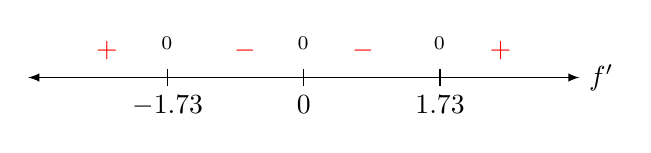
\begin{tikzpicture}
\draw[latex-latex] (-3.5,0) -- (3.5,0) node[right]{$f'$} ; %edit here for the axis
%\draw [very thick, - latex, blue] (0,0) -- (2.5,0);
%\node[circle,draw=blue, fill=blue, inner sep=0pt,minimum size=5pt] (a) at (0,0) {};
\foreach \x in  {-1.73, 0,1.73} % edit here for the vertical lines
\draw[shift={(\x,0)},color=black] (0pt,3pt)  node[above] {$^0$} -- (0pt,-3pt);
\foreach \x in  {-1.73, 0,1.73}  % edit here for the numbers
\draw[shift={(\x,0)},color=black] (0pt,0pt) -- (0pt,-3pt) node[below] 
{$\x$};
\foreach \x in  {-2.5, 2.5}  % edit here for +'s
\draw[shift={(\x,3pt)},color=red] node[above] {$+$};
\foreach \x in  {-0.75, 0.75}  % edit here for -'s
\draw[shift={(\x,3pt)},color=red] node[above] {$-$};
\end{tikzpicture}
\end{center}

We see that $f$ is increasing on $(-\infty,-\sqrt{3})\cup(\sqrt{3},\infty)$ and $f$ is decreasing on $(-\sqrt{3},0)\cup(0,\sqrt{3})$. $f$ has a local maximum at $x=-\sqrt{3}$ and a local minimum at $x=\sqrt{3}$, and neither a minimum nor a maximum at $x=0$. 

\item Next, we investigate concavity and inflection points. Differentiating, $f'(x) = 3x^4-9x^2$, we see that 
$$f''(x) = 12x^3-18x.$$ 
Since we are interested in knowing the intervals on which $f''$ is positive and negative, we find where $f''(x) = 0$:
$$0 = 12x^3-18x = 12x\left(x^2-\frac{3}{2}\right) = 12x\left(x+\sqrt{\frac{3}{2}}\right)\left(x-\sqrt{\frac{3}{2}}\right).$$
This equation has solutions $x=0$ and $x= \pm\sqrt{\frac{3}{2}}\approx1.22$. Building a sign chart for $f''$, we see

%%%%%%%%%%%%%%
%%%%%%%%Number line
%%%%%%%%%%%%%%
\begin{center}
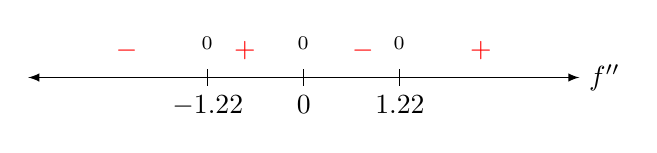
\begin{tikzpicture}
\draw[latex-latex] (-3.5,0) -- (3.5,0) node[right]{$f''$} ; %edit here for the axis
%\draw [very thick, - latex, blue] (0,0) -- (2.5,0);
%\node[circle,draw=blue, fill=blue, inner sep=0pt,minimum size=5pt] (a) at (0,0) {};
\foreach \x in  {-1.22, 0,1.22} % edit here for the vertical lines
\draw[shift={(\x,0)},color=black] (0pt,3pt)  node[above] {$^0$} -- (0pt,-3pt);
\foreach \x in  {-1.22, 0,1.22}  % edit here for the numbers
\draw[shift={(\x,0)},color=black] (0pt,0pt) -- (0pt,-3pt) node[below] 
{$\x$};
\foreach \x in  {-0.75, 2.25}  % edit here for +'s
\draw[shift={(\x,3pt)},color=red] node[above] {$+$};
\foreach \x in  {-2.25, 0.75}  % edit here for -'s
\draw[shift={(\x,3pt)},color=red] node[above] {$-$};
\end{tikzpicture}
\end{center}

Therefore $f$ is concave down on $\left(-\infty,-\sqrt{\frac{3}{2}}\right)\cup\left(0,\sqrt{\frac{3}{2}}\right)$ and concave up on $\left(-\sqrt{\frac{3}{2}},0\right)\cup\left(\sqrt{\frac{3}{2}},\infty\right)$. There are inflection points at $x=0, \pm\sqrt{\frac{3}{2}}$. 
\end{enumerate}

Putting all of this information together, we get a fairly accurate possible graph of $f(x)$, despite not knowing any of the actual $y$-values of $f(x)$. 
\begin{itemize}
\item There is a local maximum at $x=-\sqrt{3}$, labeled with the letter $A$.
\item There is an inflection point at $x=-\sqrt{3/2}$, labeled with the letter $B$.
\item There is an inflection point at $x=0$, labeled with the letter $C$.
\item There is an inflection point at $x=\sqrt{3/2}$, labeled with the letter $D$. 
\item There is a local minimum at $x=\sqrt{3}$, labeled with the letter $E$. 
\end{itemize}

\begin{figure}[H]
\centering
\includegraphics[width=3.5in]{ACFigure3-1-13.png}
\caption{An approximate graph of $f(x)$, without any precise $y$-values but correct relative positions.}
\end{figure}

\end{example}


\begin{exercise}
Determine a potential formula for $f(x)$ from Example \autoref{ex:unknownquintic}, based only on the knowledge that 
$$f'(x) = 3x^4-9x^2.$$
There are many different possible formulas. Double-check that your function $f(x)$ really does have the correct first derivative, then use it to complete steps (a)-(f) of the curve sketch summary that we skipped in Example \autoref{ex:unknownquintic}. Lastly, find the precise $y$-values using your formula for $f(x)$ and sketch the graph of $f(x)$ using those $y$-values. If you have done everything correctly, it should have the same overall shape as the graph at the end of Example \autoref{ex:unknownquintic}. 
\end{exercise}






\subsection{Some  general observations about graphs of polynomials}

We discussed in \autoref{sec:polyandratfuncs} that the degree of a polynomial determines an upper bound for the number of its $x$-intercepts and also of its turning points, a.k.a. local maxima and minima; revisit Theorem \autoref{thm:graphsofpolynomials1} if you do not remember. It turns out that the $x$-intercepts of the polynomial can give us a lower bound for the number of turning points. 

By the Mean Value Theorem (Theorem \ref{thm:meanvaluetheorem}), between every two $x$-intercepts of a polynomial $f(x)$ must lie at least one zero of its derivative (where $f'(c)=0$). In fact, we can guarantee even more: Between each adjacent pair of $x$-intercepts of $f(x)$ there must be some zero of $f'(x)$ at which the graph of $f(x)$ actually turns around and has a local maximum or minimum value. This observation is summarized in the following useful theorem:

\begin{theorem}[Turning Points Between Zeros of Polynomials]\label{thm:turningpointsofpolys}
If $f$ is a polynomial function of degree $n$ with $k$ real zeros, then $f$ has at least $k-1$ turning points, with at least one turning point between each zero. 
\end{theorem}

As a corollary (in other words, an immediate consequence) to this theorem, notice that if a polynomial of degree $n$ splits into $n$ distinct linear factors, then it will have the maximum number $n$ of $x$-intercepts and also the maximum number $n-1$ of turning points, one between and/or at each $x$-intercept. If the polynomial splits into $k$ linear factors, some of which are repeated, then it will have exactly $k-1$ turning points, one between each $x$-intercept.

You do not need to memorize these results, but they are useful in checking that your sign analyses for your first derivatives are correct. 


%
%
%\subsection*{Summary}
%The following method was introduced in this section: 
%\begin{quotation}
%Curve Sketching Summary for Polynomial Functions
%\end{quotation}
%
%\textbf{Key ideas:} In order to graph a polynomial function by hand, we determine the domain, intercepts, symmetry, end-behavior, and first- and second-derivative information for the function. We plot key points (intercepts, local extrema, inflection points), summarize the behavior of the graph between each point (increasing/decreasing, concave up/down), and then connect the points using the four possible shapes of nonlinear functions. 
%
%\textbf{Other ideas reinforced/introduced:}  A polynomial function must have a local minimum or maximum between each of its $x$-intercepts. Using only information about the first and second derivative of a function, we can still get a remarkably accurate graph without knowing any precise $y$-values. 
%
%
%
%
%
%\begin{center}
%\textcolor{ocre}{\fbox{\fbox{\Large \bf \sc End of Section 4.6}}}
%\end{center}
%
%\hspace{-.5in}\rule{1.1\textwidth}{2pt}
%
%
%




%
%\subsection{Curve Sketching with Rational Functions}\label{sec:curvesketchingwithasymptotes}
%
%
%\subsection*{Learning Goals}
%
%\begin{itemize}
%	\item   Follow the Curve Sketching Summary: Rational Functions method to construct an accurate, labeled graph of a rational function. 
%	\item Recall how to determine vertical asymptotes, holes, and horizontal asymptotes via limit calculations. 
%	\item Reflect on the information collected in the various steps of the method and whether they support or contradict each other. 
%\end{itemize}

%\subsection{Curve Sketching Summary: Rational Functions}
%
%In this section, we add a few more items to our check-list of features to identify when sketching graphs of functions. Because we expand from polynomial to rational functions, we must be concerned with identifying any points where the function is undefined and determining the behavior of the function at those points via limits (either finding a hole or a vertical asymptote). Additionally, the end-behavior of rational functions may be infinite, or the function may have a horizontal asymptote. When sketching a graph of a rational function, you should include:
%
%\begin{enumerate}[label=\textbf{\alph*.},itemsep=5pt,topsep=5pt]
%\item the domain.
%\item the $y$-intercept. 
%\item any $x$-intercepts that we can find easily (many times this is not possible without more advanced algebraic methods). Potentially a sign analysis for the function itself that shows where it is above and below the $x$-axis, but this requires complete knowledge of all $x$-intercepts. 
%\item any even or odd symmetry. 
%\item the behavior of the function at any non-domain points, meaning the limits as $x\to c$ for any value $x=c$ not in the domain of the function. We make special note of any holes or vertical asymptotes. 
%\item the "end behavior" of the graph, meaning the limits as $x\to\pm\infty$. We make special note of any horizontal asymptotes. 
%\item any local minima or maxima, along with  where the function is increasing and decreasing using the first derivative. 
%\item any inflection points and where the function is concave up and concave down using the second derivative. 
%\end{enumerate}
%
%To begin graphing the function, we first plot all of the intercepts, holes, local minima and maxima, and inflection points. We draw dashed vertical lines for any vertical asymptotes, and dashed horizontal lines for any horizontal asymptotes. Then we "connect the dots" using the following four possible shapes of nonlinear functions:
%
%\begin{center}
%\includegraphics[width=5in]{TaalmanPage250.png}
%\end{center}

\subsection{Reviewing Asymptotes and Limit Calculations}

Hopefully you remember how to find holes, vertical asymptotes, and horizontal asymptotes. If not, revisit the appropriate section below based on the information you have forgotten:

\begin{itemize}[itemsep=5pt]
\item Vertical and horizontal asymptotes are defined in \autoref{sec:VAsandHAs}. 
\item Calculating limits of the form $\frac{1}{0}$ is discussed in \autoref{sec:oneoverzerolimits}. 
\item Calculating limits of the form $\frac{0}{0}$ is discussed in \autoref{sec:zerooverzerolimits}.
\item Distinguishing between holes and vertical asymptotes is discussed in \autoref{sec:holeorVA}.
\item Determining end-behavior of rational functions is discussed in \autoref{sec:endbehaviorofrationalfunctions}. In particular, this section covers how to evaluate $\frac{\infty}{\infty}$ limits. 
\end{itemize}



\subsection{Examples of Sketching Rational Functions}\label{sec:curvesketchingwithasymptotes}


\begin{example}\label{ex:rationalsketch1}
For the first example, we sketch the graph of the function 
$$f(x) = \dfrac{x}{1+x^2}.$$


\begin{enumerate}[label=\textbf{\alph*.},itemsep=5pt,topsep=5pt]
\item 
%the domain.
$f(x) = \frac{x}{1+x^2}$  is defined for all real numbers since $1+x^2$ is never equal to zero. Indeed, if we try to solve for values of $x$ that make the denominator zero:
$$\begin{aligned}
1+x^2 &= 0\\
x^2 &= -1
\end{aligned}$$
we can see that there are no such $x$-values since the square of any number must be 0 or positive. Alternately, if we tried to take the square root of both sides, we would be taking the square root of a negative number, which is not possible (in this class). Thus the domain of $f(x)$ is
$$(-\infty,\infty).$$

\item 
%the $y$-intercept. 
The $y$-intercept of $f(x) = \frac{x}{1+x^2}$ is $y=f(0) = \frac{0}{1+0^2} = \frac{0}{1} = 0$, so at the point $(0,0)$. 

\item 
%any $x$-intercepts that we can find easily (many times this is not possible without more advanced algebraic methods). Potentially a sign analysis for the function itself that shows where it is above and below the $x$-axis, but this requires complete knowledge of all $x$-intercepts. 
$f(x)$ is equal to zero when its numerator is equal to zero, so when $x=0$. Thus we see that the only $x$-intercept of $f(x)$ is the same point $(0,0)$ that we found as the $y$-intercept. Since we have been able to find all of the $x$-intercepts and points where $f(x)$ is undefined, we can create a sign analysis for $f(x)$: 

%%%%%%%%%%%%%%
%%%%%%%%Number line
%%%%%%%%%%%%%%
\begin{center}
\begin{tikzpicture}
\draw[latex-latex] (-3,0) -- (3,0) node[right] {$f$} ; %edit here for the axis
%\draw [very thick, - latex, blue] (0,0) -- (2.5,0);
%\node[circle,draw=blue, fill=blue, inner sep=0pt,minimum size=5pt] (a) at (0,0) {};
\foreach \x in  { 0} % edit here for the vertical lines
\draw[shift={(\x,0)},color=black] (0pt,3pt) -- (0pt,-3pt);
\foreach \x in  {0}  % edit here for the numbers
\draw[shift={(\x,0)},color=black] (0pt,0pt) -- (0pt,-3pt) node[below] {$\x$};
\foreach \x in  {0}  % edit here for 0's
\draw[shift={(\x,3pt)}] node[above] {$^0$};
%\foreach \x in  {-1, 2}  % edit here for DNE's
%\draw[shift={(\x,3pt)}] node[above] {$^\text{DNE}$};
\foreach \x in  {1.5}  % edit here for +'s
\draw[shift={(\x,3pt)},color=red] node[above] {$+$};
\foreach \x in  {-1.5}  % edit here for -'s
\draw[shift={(\x,3pt)},color=red] node[above] {$-$};
\end{tikzpicture}
\end{center}


\item 
%any even or odd symmetry. 
We check whether $f(-x) = f(x)$ or $f(-x)=-f(x)$, or neither:
$$f(-x) = \frac{-x}{1+(-x)^2} = \frac{-x}{1+x^2} = -\,\frac{x}{x^2+1} = -f(x).$$
Hence $f(x)$ is odd and so has $180^\circ$ rotational symmetry about the origin. 


\item 
%the behavior of the function at any non-domain points, meaning the limits as $x\to c$ for any value $x=c$ not in the domain of the function. We make special note of any holes or vertical asymptotes. 
Because $f(x)$ is rational, thus algebraic, and is defined for all real numbers, it is also continuous for all real numbers, and thus cannot have any vertical asymptotes or holes. 

\item 
%the "end behavior" of the graph, meaning the limits as $x\to\pm\infty$. We make special note of any horizontal asymptotes. 
The limits as $x\to\pm \infty$ of $f(x)$ are both indeterminate of the form $\frac{\infty}{\infty}$ and so require algebraic methods to evaluate. Dividing through by $x^2$:
$$\begin{aligned}
\lim_{x\to\infty}\frac{x}{1+x^2} \cdot\frac{\frac{1}{x^2}}{\frac{1}{x^2}}&=\lim_{x\to\infty}\frac{\frac{1}{x}}{\frac{1}{x^2}+1}\\
&= \frac{0}{0+1}=0
\end{aligned}$$
Similarly, 
$$\begin{aligned}
\lim_{x\to-\infty}\frac{x}{1+x^2} &=\lim_{x\to-\infty}\frac{\frac{1}{x}}{\frac{1}{x^2}+1}\\
&= \frac{0}{0+1}=0
\end{aligned}$$
Thus $f(x)$ has right and left horizontal asymptotes at $y=0$. 


\item %any local minima or maxima, along with  where the function is increasing and decreasing using the first derivative. 
Moving on to the first derivative:
$$\begin{aligned}
f'(x) &= \frac{(1+x^2)(1)-(x)(2x)}{(1+x^2)^2}\\
&= \frac{1-x^2}{(1+x^2)^2}
\end{aligned}$$
$f'(x) = 0$ when $1-x^2 = (1-x)(1+x) = 0$. $f'(x)$ is never undefined as we have already noted that $1+x^2$ is never zero. Thus $f$ has critical points at $x=\pm1$. The sign analysis for $f'$ is 
%%%%%%%%%%%%%%
%%%%%%%%Number line
%%%%%%%%%%%%%%
\begin{center}
\begin{tikzpicture}
\draw[latex-latex] (-3,0) -- (3,0) node[right] {$f'$} ; %edit here for the axis
\foreach \x in  { -1,1} % edit here for the vertical lines
\draw[shift={(\x,0)},color=black] (0pt,3pt) -- (0pt,-3pt);
\foreach \x in  {-1,1}  % edit here for the numbers
\draw[shift={(\x,0)},color=black] (0pt,0pt) -- (0pt,-3pt) node[below] {$\x$};
\foreach \x in  {-1,1}  % edit here for 0's
\draw[shift={(\x,3pt)}] node[above] {$^0$};
%\foreach \x in  {-1, 2}  % edit here for DNE's
%\draw[shift={(\x,3pt)}] node[above] {$^\text{DNE}$};
\foreach \x in  {0}  % edit here for +'s
\draw[shift={(\x,3pt)},color=red] node[above] {$+$};
\foreach \x in  {-2,2}  % edit here for -'s
\draw[shift={(\x,3pt)},color=red] node[above] {$-$};
\end{tikzpicture}
\end{center}
Thus $f$ is decreasing on $(-\infty,-1)$ and $(1,\infty)$ and increasing on $(-1,1)$. There is a local minimum at $x=-1$ where $y=f(-1) = \frac{-1}{1+(-1)^2} = -\frac{1}{2}$. There is a local maximum at $x=1$ where $y=f(1) = \frac{1}{1+(1)^2} = \frac{1}{2}$.


\item %any inflection points and where the function is concave up and concave down using the second derivative. 

We calculate the second derivative, being careful to factor as much as possible:
$$\begin{aligned}
f''(x) &= \frac{(1+x^2)^2(-2x) - (1-x^2)(2(1+x^2)(2x))}{((1+x^2)^2)^2}\\
&= \frac{(1+x^2)(2x)\big[(1+x^2)(-1)-(1-x^2)(2)\big]}{(1+x^2)^4}\\
&= \frac{2x(-1-x^2-2+2x^2)}{(1+x^2)^3}\\
&= \frac{2x(x^2-3)}{(1+x^2)^3}\\
\end{aligned}$$
$f''(x)=0$ when $2x(x^2-3)=0$, so when $x=0$ or $x^2-3=0$. Solving this last equation, $x^2=3$, meaning $x=\pm\sqrt{3}\approx 1.732$. $f''(x)$ is never undefined as we have already noted that $1+x^2$ is never zero. Thus $f'$ has critical points at $x=0,\pm\sqrt{3}$, that may or may not be inflection points. The sign chart for $f''$ is 
%%%%%%%%%%%%%%
%%%%%%%%Number line
%%%%%%%%%%%%%%
\begin{center}
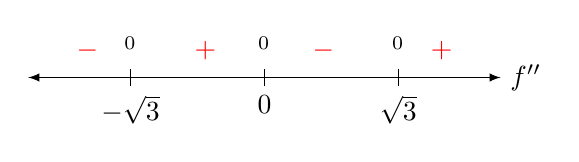
\begin{tikzpicture}
\draw[latex-latex] (-3,0) -- (3,0) node[right] {$f''$} ; %edit here for the axis
\foreach \x in  { -1.7,0,1.7} % edit here for the vertical lines
\draw[shift={(\x,0)},color=black] (0pt,3pt) -- (0pt,-3pt);
\foreach \x in  {0}  % edit here for the numbers
\draw[shift={(\x,0)},color=black] (0pt,0pt) -- (0pt,-3pt) node[below] {$\x$};
\draw[shift={(-1.7,0)},color=black] (0pt,0pt) -- (0pt,-3pt) node[below] {$-\sqrt{3}$};
\draw[shift={(1.7,0)},color=black] (0pt,0pt) -- (0pt,-3pt) node[below] {$\sqrt{3}$};
\foreach \x in  {-1.7,0,1.7}  % edit here for 0's
\draw[shift={(\x,3pt)}] node[above] {$^0$};
%\foreach \x in  {-1, 2}  % edit here for DNE's
%\draw[shift={(\x,3pt)}] node[above] {$^\text{DNE}$};
\foreach \x in  {-0.75, 2.25}  % edit here for +'s
\draw[shift={(\x,3pt)},color=red] node[above] {$+$};
\foreach \x in  {-2.25,0.75}  % edit here for -'s
\draw[shift={(\x,3pt)},color=red] node[above] {$-$};
\end{tikzpicture}
\end{center}
Hence $f$ is concave down on $(-\infty,-\sqrt{3})$ and $(0,\sqrt{3})$ and is concave up on $(-\sqrt{3},0)$ and $(\sqrt{3},\infty)$. $f$ has inflection points at $x=0$ where $y=f(0)=0$, at $x=-\sqrt{3}$ where $y=f(-\sqrt{3}) = \frac{-\sqrt{3}}{1+(-\sqrt{3})^2} = -\frac{\sqrt{3}}{4}\approx -0.433$, and at $x=\sqrt{3}$ where $y=f(\sqrt{3}) = \frac{\sqrt{3}}{1+(\sqrt{3})^2} = \frac{\sqrt{3}}{4}\approx 0.433$. 
\end{enumerate}



 


We first plot all of the key points and features found:
\begin{itemize}
\item \textbf{Intercepts} $(0,0)$
\item \textbf{Asymptotes and/or Holes} Horizontal asymptote at $y=0$ to the right and left. 
\item \textbf{Local extrema} Maximum  at $(1,1/2)$ and minimum at $(-1,-1/2)$
\item \textbf{Inflection points} $(-\sqrt{3},-\sqrt{3}/4)\approx (-1.732,-0.433), \quad (0,0),\quad (\sqrt{3},\sqrt{3}/4)\approx (1.732,0.433)$
\end{itemize}

Next, we determine which of the four shapes the graph has between each of these points based on whether the graph is increasing/decreasing and concave up/down. This information is summarized in the table below:

\begin{table}[H]
\centering
\begin{tabular}{| l | c|c|c|c|c|c|}
\hline
Interval & $(-\infty,-\sqrt{3})$ & $(-\sqrt{3},-1)$ & $(-1,0)$ & $(0,1)$ & $(1,\sqrt{3})$ &  $(\sqrt{3},\infty)$\\
\hline
\hline
$f'$ is\ldots & $-$ & $-$ & $+$ & $+$ & $-$ & $-$\\
$f$  is\ldots & dec &  dec & inc & inc & dec & dec\\
\hline
$f''$  is\ldots & $-$  & $+$ & $+$ & $-$ & $-$ & $+$ \\
$f$ is\ldots & ccd & ccu & ccu & ccd & ccd & ccu \\
\hline
\end{tabular}
\end{table}

Completing the graph:

\begin{center}
\includegraphics[width=4in]{4-7Example1Graph.png}
\end{center}

We note that this does appear to have the odd symmetry we found (and could have used to find some of the $y$-values). 

\end{example}

\begin{exercise}
Use the second derivative test to confirm that $f(x) = \frac{x}{1+x^2}$ from Example \autoref{ex:rationalsketch1} has a local minimum at $x=-1$ and a local maximum at $x=1$. \textit{Remember: there are often multiple ways to determine the same answer, and all of the different methods should agree with each other.}
\end{exercise}




\begin{example}\label{ex:rationalsketch2}
Consider the function 
$$g(x) = \frac{x^2}{x^2-2x+1}.$$


\begin{enumerate}[label=\textbf{\alph*.},itemsep=5pt,topsep=5pt]
\item 
%the domain.
Factoring the denominator of $g(x)$:
$$g(x) = \frac{x^2}{x^2-2x+1}. = \frac{x^2}{(x-1)(x-1)} = \frac{x^2}{(x-1)^2},$$
$g(x)$ is undefined when its denominator is equal to zero, so we see that $g(x)$ is undefined at $x=1$. Thus $g(x)$ has domain $(-\infty,1)\cup(1,\infty)$. 

\item 
%the $y$-intercept. 
$g(x)$ has $y$-intercepts $y=g(0) = \frac{0^2}{0^2-2(0)+1} = \frac{0}{1} = 0$, so at the point $(0,0)$. 


\item 
%any $x$-intercepts that we can find easily (many times this is not possible without more advanced algebraic methods). Potentially a sign analysis for the function itself that shows where it is above and below the $x$-axis, but this requires complete knowledge of all $x$-intercepts. 
The $x$-intercept of $g(x)$ is where its numerator, $x^2$, is equal to zero, so when $x=0$. Thus the only $x$-intercept is the point $(0,0)$ that is also the $y$-intercept. 

Since we can rewrite $g(x) = \dfrac{x^2}{(x-1)^2}$, we can tell without a sign analysis that $g(x)$ will always be above the $x$-axis when it is not equal to zero. This is because both the numerator and denominator are squared, hence cannot be negative. 

\item 
%any even or odd symmetry. 
Simplifying $g(-x)$:
$$\begin{aligned}
g(-x) &= \frac{(-x)^2}{(-x)^2-2(-x)+1}\\
&= \frac{x^2}{x^2+2x+1}
\end{aligned}$$
we see that $g(x)$ is neither even nor odd since $g(-x)\neq g(x)$ and $g(-x)\neq -g(x)$. 


\item 
%the behavior of the function at any non-domain points, meaning the limits as $x\to c$ for any value $x=c$ not in the domain of the function. We make special note of any holes or vertical asymptotes. 
$g(x)$ is undefined at $x=1$ where the denominator is equal to 0, so we suspect that it has a vertical asymptote there. Calculating the limit as $x\to 1$ explicitly:
$$\lim_{x\to 1}g(x) = \lim_{x\to 1}\frac{x^2}{(x-1)^2} = \frac{1}{0^+} = \infty$$
where we know that the denominator must be positive without taking right and left limits separately because $(x-1)^2>0$ for all $x$.%\footnote{Remember that even powers of numbers must be nonnegative.}

\item 
%the "end behavior" of the graph, meaning the limits as $x\to\pm\infty$. We make special note of any horizontal asymptotes. 
We calculate $\lim_{x\to\pm\infty}$ by force-factoring $x^2$ from the denominator, since both limits have the indeterminate form $\frac{\infty}{\infty}$:
$$\begin{aligned}
\lim_{x\to\infty}\frac{x^2}{x^2-2x+1} &= \lim_{x\to\infty}\frac{x^2}{x^2\left(1-\frac{2}{x}+\frac{1}{x^2}\right)}\\
&=\lim_{x\to\infty}\frac{1}{1-\frac{2}{x}+\frac{1}{x^2}} \\
&= \frac{1}{1-0-0}= 1
\end{aligned}$$
and similarly, 
$$\begin{aligned}
\lim_{x\to-\infty}\frac{x^2}{x^2-2x+1} &= \lim_{x\to-\infty}\frac{x^2}{x^2\left(1-\frac{2}{x}+\frac{1}{x^2}\right)}\\
&=\lim_{x\to-\infty}\frac{1}{1-\frac{2}{x}+\frac{1}{x^2}} \\
&= \frac{1}{1-0-0}= 1
\end{aligned}$$
Thus $g(x)$ has a horizontal asymptote at $y=1$ to the right and left. 

\item 
%any local minima or maxima, along with  where the function is increasing and decreasing using the first derivative. 
Now let's examine the first derivative. We use the quotient rule:
$$\begin{aligned}
g'(x) &= \frac{(x^2-2x+1)(2x)-(x^2)(2x-2)}{(x^2-2x+1)^2} \\
&= \frac{-2x^2+2x}{((x-1)^2)^2} \\
&= \frac{-2x(x-1)}{(x-1)^4} \\
&= \frac{-2x}{(x-1)^3}
\end{aligned}$$
$g'(x)$ is zero when its numerator is zero, meaning when $x=0$. It is undefined when its denominator is zero, so when $x=1$. Only $x=0$ is a critical point, but $g'(x)$ may change sign at either $x=0$ or $x=1$ and so we put both on the number line for $g'(x)$:
%%%%%%%%%%%%%%
%%%%%%%%Number line
%%%%%%%%%%%%%%
\begin{center}
\begin{tikzpicture}
\draw[latex-latex] (-3,0) -- (3,0) node[right] {$g'$} ; %edit here for the axis
\foreach \x in  { 0,1} % edit here for the vertical lines
\draw[shift={(\x,0)},color=black] (0pt,3pt) -- (0pt,-3pt);
\foreach \x in  {0,1}  % edit here for the numbers
\draw[shift={(\x,0)},color=black] (0pt,0pt) -- (0pt,-3pt) node[below] {$\x$};
\foreach \x in  {0}  % edit here for 0's
\draw[shift={(\x,3pt)}] node[above] {$^0$};
\foreach \x in  {1}  % edit here for DNE's
\draw[shift={(\x,3pt)}] node[above] {$^\text{DNE}$};
\foreach \x in  {0.5}  % edit here for +'s
\draw[shift={(\x,3pt)},color=red] node[above] {$+$};
\foreach \x in  {-2,2}  % edit here for -'s
\draw[shift={(\x,3pt)},color=red] node[above] {$-$};
\end{tikzpicture}
\end{center}
So $g(x)$ is decreasing on $(-\infty,0)$ and $(1,\infty)$ and increasing on $(0,1)$. Note that this confirms that both sides of the vertical asymptote at $x=1$ approach $+\infty$. $g(x)$ has local minimum at the critical point $x=0$ where $y=0$, so at the $x$- and $y$-intercept that we found earlier.

 
\item 
%any inflection points and where the function is concave up and concave down using the second derivative. 
Now let's move on to the second derivative, remembering to factor as much as possible at every step:
$$\begin{aligned}
g''(x) &= \frac{(x-1)^3(-2)-(-2x)(3(x-1)^2)}{((x-1)^3)^2}\\
&= \frac{(-2)(x-1)^2\big[(x-1)-(x)(3)\big]}{(x-1)^6}\\
&= \frac{-2(x-1-3x)}{(x-1)^4}\\
&=\frac{-2(-2x-1)}{(x-1)^4}\\
&=\frac{2(2x+1)}{(x-1)^4}
\end{aligned}$$
$g''(x)$ is equal to zero when $2(2x+1)=0$ so when $x=-\frac{1}{2}$ and is undefined when $x=1$, as expected. The critical point for $g'(x)$ is $x=-\frac{1}{2}$ and NOT $x=1$, since $g'(x)$ was also undefined when $x=1$. The sign analysis for $g''(x)$ is:

%%%%%%%%%%%%%%
%%%%%%%%Number line
%%%%%%%%%%%%%%
\begin{center}
\begin{tikzpicture}
\draw[latex-latex] (-3,0) -- (3,0) node[right] {$g''$} ; %edit here for the axis
\foreach \x in  { -1,2} % edit here for the vertical lines
\draw[shift={(\x,0)},color=black] (0pt,3pt) -- (0pt,-3pt);
\foreach \x in  {-0.5,1}  % edit here for the numbers
\draw[shift={(2*\x,0)},color=black] (0pt,0pt) -- (0pt,-1.5pt) node[below] {$\x$};
\foreach \x in  {-1}  % edit here for 0's
\draw[shift={(\x,3pt)}] node[above] {$^0$};
\foreach \x in  {2}  % edit here for DNE's
\draw[shift={(\x,3pt)}] node[above] {$^\text{DNE}$};
\foreach \x in  {0.5, 2.5}  % edit here for +'s
\draw[shift={(\x,3pt)},color=red] node[above] {$+$};
\foreach \x in  {-1.5}  % edit here for -'s
\draw[shift={(\x,3pt)},color=red] node[above] {$-$};
\end{tikzpicture}
\end{center}
Thus $g(x)$ is concave down on $\left(-\infty,-\frac{1}{2}\right)$ and is concave up on $\left(-\frac{1}{2},1\right)$ and on $(1,\infty)$. There is an inflection point at $x=-\frac{1}{2}$ where $y=f\left(-\frac{1}{2}\right) = \frac{\left(-\frac{1}{2}\right)^2}{(1+\frac{1}{2})^2} = \frac{1/4}{9/4} = \frac{1}{9}$. 
\end{enumerate}



We first plot all of the key points and features found:
\begin{itemize}
\item \textbf{Intercepts} $(0,0)$
\item \textbf{Asymptotes and/or Holes} Vertical asymptote to $\infty$ at $x=1$. Horizontal asymptote at $y=1$ to the right and left. 
\item \textbf{Local extrema} Minimum at $(0,0)$.
\item \textbf{Inflection points} $(-1/2, 1/9)\approx (-0.5,0.1111)$
\end{itemize}

Next, we determine which of the four shapes the graph has between each of these points based on whether the graph is increasing/decreasing and concave up/down. This information is summarized in the table below:

\begin{table}[H]
\centering
\begin{tabular}{| l | c|c|c|c|}
\hline
Interval & $(-\infty,-1/2)$ & $(-1/2,0)$ & $(0,1)$ & $(1,\infty)$\\
\hline
\hline
$g'$ is\ldots & $-$ & $-$ & $+$ & $-$ \\
$g$  is\ldots & dec &  dec & inc & dec\\
\hline
$g''$  is\ldots & $-$  & $+$ & $+$ & $+$ \\
$g$ is\ldots & ccd & ccu & ccu & ccu \\
\hline
\end{tabular}
\end{table}

Completing the graph:

\begin{center}
\includegraphics[width=5in]{4-7Example2Graph.png}
\end{center}


\end{example}

\begin{exercise}
\textit{Conjecture:} In both Example \autoref{ex:rationalsketch1} and Example \autoref{ex:rationalsketch2}, the rational functions had the same horizontal asymptotes to the right and left. Do you think it is always the case that a rational function with a horizontal asymptote will have the same value for both $x\to\infty$ and $x\to-\infty$? Why or why not?
\end{exercise}

The last function we sketch will be significantly complicated in order to illustrate some of the other types of behaviors you are likely to see when sketching rational functions. If you are already feeling fatigued, it's probably a good idea to take a break before returning to read this last example. 


\begin{example}
Consider the function 
$$h(x) = \frac{2(x-1)^2(x+2)}{(x-1)(x+1)(x-2)}.$$


\begin{enumerate}[label=\textbf{\alph*.},itemsep=5pt,topsep=5pt]
\item 
%the domain.
$h(x)$ is undefined when its denominator is equal to zero, thus when 
$$(x-1)(x+1)(x-2) = 0 \quad\Longleftrightarrow\quad x=-1, 1, 2$$
The domain of $h(x)$ is 
$$(-\infty,-1)\cup(-1,1)\cup(1,2)\cup (2,\infty).$$


\item 
%the $y$-intercept. 
The $y$-intercept of $h(x)$ is at
$$y = h(0) = \frac{2(-1)^2(2)}{(-1)(1)(-2)} = \frac{4}{2} = 2,$$
meaning at the point $(0,2)$. 



\item 
%any $x$-intercepts that we can find easily (many times this is not possible without more advanced algebraic methods). Potentially a sign analysis for the function itself that shows where it is above and below the $x$-axis, but this requires complete knowledge of all $x$-intercepts. 
The $x$-intercepts of $h(x)$ are when the numerator is equal to zero, but we must be careful to also stay in the domain of the function. 
$$2(x-1)^2(x+2)=0 \quad\Longleftrightarrow\quad x=-2,1$$
but $h(1)$ is undefined. Thus the only $x$-intercept of $h(x)$ is at the point $(-2,0)$. 

A  sign analysis of $h(x)$ tells us where the graph of $h(x)$ is above or below the $x$-axis. We must check the sign of $h(x)$ on each subinterval between the $x$-intercept and non-domain points:
%%%%%%%%%%%%%%
%%%%%%%%Number line
%%%%%%%%%%%%%%
\begin{center}
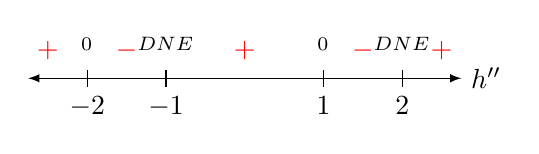
\begin{tikzpicture}
\draw[latex-latex] (-2.75,0) -- (2.75,0) node[right] {$h''$} ; %edit here for the axis
%\draw [very thick, - latex, blue] (0,0) -- (2.5,0);
%\node[circle,draw=blue, fill=blue, inner sep=0pt,minimum size=5pt] (a) at (0,0) {};
\foreach \x in  {-2, -1, 1, 2} % edit here for the vertical lines
\draw[shift={(\x,0)},color=black] (0pt,3pt) -- (0pt,-3pt);
\foreach \x in  {-2, -1, 1, 2}  % edit here for the numbers
\draw[shift={(\x,0)},color=black] (0pt,0pt) -- (0pt,-3pt) node[below] 
{$\x$};
\foreach \x in  {-2, 1}  % edit here for 0's
\draw[shift={(\x,3pt)}] node[above] {$^0$};
\foreach \x in  {-1, 2}  % edit here for DNE's
\draw[shift={(\x,3pt)}] node[above] {$^\text{DNE}$};
\foreach \x in  {-2.5, 0, 2.5}  % edit here for +'s
\draw[shift={(\x,3pt)},color=red] node[above] {$+$};
\foreach \x in  {-1.5, 1.5}  % edit here for -'s
\draw[shift={(\x,3pt)},color=red] node[above] {$-$};
\end{tikzpicture}
\end{center}




\item 
%any even or odd symmetry. 
Comparing $h(-x)$ to $h(x)$ and $-h(x)$ is quite challenging with $h(x)$ factored as it is. The best way to determine whether $h(x)$ is even or odd is to first expand $h(x)$:
$$\begin{aligned}
h(x) &= \frac{2(x-1)^2(x+2)}{(x-1)(x+1)(x-2)}\\
&= \frac{2 x^3 - 6 x + 4}{x^3 - 2 x^2 - x + 2}
\end{aligned}$$
and then simplify $h(-x)$ to compare it to $h(x)$ and $-h(x)$:
$$\begin{aligned}
h(-x) &= \frac{2(-x)^3-6(-x)+4}{(-x)^3-2(-x)^2-(-x)+2}\\
&= \frac{-2x^3+6x+4}{-x^3-2x^2+x+2}
\end{aligned}$$
We can see that $h(-x)$ is not equal to $h(x)$ as it is written, and also checking that it still is not equal after factoring and cancelling a $-1$ from both the numerator and denominator:
$$h(-x) = \frac{-(2x^3-6x-4)}{-(x^3+2x^2-x-2)} = \frac{2x^3-6x-4}{x^3+2x^2-x-2}.$$
Thus $h(x)$ is not even. $h(-x)$ is also not equal to $-h(x)$, which we could write in any of the following forms:
$$\begin{aligned}
-h(x) &= -\,\frac{2 x^3 - 6 x + 4}{x^3 - 2 x^2 - x + 2} \\
& = \frac{-2x^3+6x-4}{x^3 - 2 x^2 - x + 2}\\
&= \frac{2 x^3 - 6 x + 4}{-x^3+2x^2+x-2}
\end{aligned}$$
Thus $h(x)$ is also not odd.


\item 
%the behavior of the function at any non-domain points, meaning the limits as $x\to c$ for any value $x=c$ not in the domain of the function. We make special note of any holes or vertical asymptotes. 
Since $h(x)$ is undefined at $x=-1, 1, $ and $2$, we must evaluate the limits at all three of these $x$-values. 

At $x=-1$:
$$
\lim_{x\to -1}\frac{2(x-1)^2(x+2)}{(x-1)(x+1)(x-2)} = \frac{2(-2)^2(1)}{(-2)(0)(-3)} = \frac{8}{0} = \pm\infty$$
and so there is a vertical asymptote at $x=-1$. In order to determine the precise behavior, we take the limits from the left and right. Note that the factor $x+1$ in the denominator is negative as $x\to -1^-$ and is positive as $x\to -1^+$:
$$\lim_{x\to -1^-}\frac{2(x-1)^2(x+2)}{(x-1)(x+1)(x-2)} = \frac{2(-2)^2(1)}{(-2)(0^-)(-3)} = \frac{8}{0^-} = -\infty$$
and
$$\lim_{x\to -1^+}\frac{2(x-1)^2(x+2)}{(x-1)(x+1)(x-2)} = \frac{2(-2)^2(1)}{(-2)(0^+)(-3)} = \frac{8}{0^+} = \infty$$

At $x=1$:
$$\lim_{x\to 1}\frac{2(x-1)^2(x+2)}{(x-1)(x+1)(x-2)} = \frac{2(0)^2(3)}{(0)(2)(-1)} = \frac{0}{0},$$
which is indeterminate. After canceling one of the factors of $x-1$ from both the numerator and denominator:
$$
\begin{aligned}
\lim_{x\to 1}\frac{2(x-1)^2(x+2)}{(x-1)(x+1)(x-2)} &= \lim_{x\to 1}\frac{2(x-1)(x+2)}{(x+1)(x-2)}\\
&=\frac{2(0)(3)}{(2)(-1)} = \frac{0}{-2}=0
\end{aligned}$$
so we see that $h(x)$ has a hole at the point $(1,0)$. 


At $x=2$:
$$
\lim_{x\to 2}\frac{2(x-1)^2(x+2)}{(x-1)(x+1)(x-2)} = \frac{2(1)^2(4)}{(3)(3)(0)} = \frac{8}{0} = \pm\infty$$
and so there is a vertical asymptote at $x=2$. In order to determine the precise behavior, we take the limits from the left and right. Note that the factor $x-2$ in the denominator is negative as $x\to 2^-$ and is positive as $x\to 2^+$:
$$
\lim_{x\to 2^-}\frac{2(x-1)^2(x+2)}{(x-1)(x+1)(x-2)} = \frac{2(1)^2(4)}{(3)(3)(0^-)} = \frac{8}{0^-} = -\infty$$
and 
$$
\lim_{x\to 2^+}\frac{2(x-1)^2(x+2)}{(x-1)(x+1)(x-2)} = \frac{2(1)^2(4)}{(3)(3)(0^+)} = \frac{8}{0^+} = \infty$$


\item 
%the "end behavior" of the graph, meaning the limits as $x\to\pm\infty$. We make special note of any horizontal asymptotes. 
The expanded form of $h(x)$ that we found earlier is simpler to use when finding the limits as $x\to\pm\infty$. Both limits have the indeterminate form $\frac{\infty}{\infty}$ and so we calculate the limits dividing through by $x^3$:
$$\lim_{x\to\infty}\frac{2 x^3 - 6 x + 4}{x^3 - 2 x^2 - x + 2} \cdot\frac{\frac{1}{x^3}}{\frac{1}{x^3}}= \lim_{x\to\infty}\frac{2-\frac{6}{x^2}+\frac{4}{x^3}}{1-\frac{2}{x}-\frac{1}{x^2}+\frac{2}{x^3}} = \frac{2}{1} = 2$$
and similarly
$$\lim_{x\to-\infty}\frac{2 x^3 - 6 x + 4}{x^3 - 2 x^2 - x + 2}\cdot\frac{\frac{1}{x^3}} = \lim_{x\to-\infty}\frac{2-\frac{6}{x^2}+\frac{4}{x^3}}{1-\frac{2}{x}-\frac{1}{x^2}+\frac{2}{x^3}} = \frac{2}{1} = 2$$
Thus $h(x)$ has a horizontal asymptote of $y=2$ to the right and left. 

\item 
%any local minima or maxima, along with  where the function is increasing and decreasing using the first derivative. 
 Since we already found the hole at $x=1$, let's work with the simplified function that results from canceling one factor of $x-1$ from the numerator and denominator:
$$h(x) = \frac{2(x-1)(x+2)}{(x+1)(x-2)} = \frac{2x^2+2x-4}{x^2-x-2}$$
Taking the first derivative using the quotient rule, simplifying, and factoring, we have:
$$\begin{aligned}
h'(x) &= \frac{(x^2-x-2)(4x+2)-(2x^2+2x-4)(2x-1)}{(x^2-x-2)^2}\\
&= \frac{(4x^3-2x^2-4x^2-2x-8x-4)-(4x^3-2x^2+4x^2-2x-8x+4)}{((x+1)(x-2))^2}\\
&= \frac{(4x^3-2x^2-10x-4)-(4x^3+2x^2-10x+4)}{(x+1)^2(x-2)^2}\\
&= \frac{-4x^2-8}{(x+1)^2(x-2)^2}\\
&= \frac{-4(x^2+2)}{(x+1)^2(x-2)^2}
\end{aligned}$$
When looking for critical points, we set both the numerator equal to zero (to determine where $h'(x)=0$) and the denominator equal to zero (to determine where $h'(x)$ is undefined). 
Setting the numerator equal to zero:
$$-4(x^2+2) = 0\quad\Longleftrightarrow \quad x^2+2 = 0 \quad\Longleftrightarrow \quad x^2 = -2$$
From this, we can see that $h'(x)\neq 0$ for any $x$-values. Setting the denominator equal to zero:
$$(x+1)^2(x-2)^2=0 \quad\Longleftrightarrow \quad x = -1,2$$
and so $h'(x)$ is undefined when $x = -1,2$. However, these are not critical points because they are not in the domain of $h(x)$. Thus $h(x)$ has no critical points. 

In the sign analysis for $h'(x)$, we must remember that $h(x)$ is undefined at $x=-1,1,$ and $2$, and so could change sign at any of those $x$-values, despite the lack of critical points:
%%%%%%%%%%%%%%
%%%%%%%%Number line
%%%%%%%%%%%%%%
\begin{center}
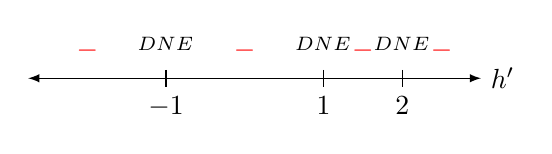
\begin{tikzpicture}
\draw[latex-latex] (-2.75,0) -- (3,0) node[right] {$h'$} ; %edit here for the axis
%\draw [very thick, - latex, blue] (0,0) -- (2.5,0);
%\node[circle,draw=blue, fill=blue, inner sep=0pt,minimum size=5pt] (a) at (0,0) {};
\foreach \x in  { -1, 1, 2} % edit here for the vertical lines
\draw[shift={(\x,0)},color=black] (0pt,3pt) -- (0pt,-3pt);
\foreach \x in  {-1, 1, 2}  % edit here for the numbers
\draw[shift={(\x,0)},color=black] (0pt,0pt) -- (0pt,-3pt) node[below] {$\x$};
%\foreach \x in  {-2, 1}  % edit here for 0's
%\draw[shift={(\x,3pt)}] node[above] {$^0$};
\foreach \x in  {-1, 1, 2}  % edit here for DNE's
\draw[shift={(\x,3pt)}] node[above] {$^\text{DNE}$};
%\foreach \x in  {-2.5, 0, 2.5}  % edit here for +'s
%\draw[shift={(\x,3pt)},color=red] node[above] {$+$};
\foreach \x in  {-2, 0, 1.5, 2.5}  % edit here for -'s
\draw[shift={(\x,3pt)},color=red] node[above] {$-$};
\end{tikzpicture}
\end{center}
We can see that since $h'(x)$ is always negative, hence $h(x)$ is always decreasing. There are no local minima or maxima. 



\item 
%any inflection points and where the function is concave up and concave down using the second derivative. 

Before we move on to the second derivative, notice that calculating derivatives of rational functions is a significant challenge, especially since we would like to be able to factor the result. Lacking more advanced algebraic techniques for factoring, a key skill to develop is to take derivatives in such a way that the result is left as factored as possible. In particular, we do not want to expand the denominator of $h'(x)$ before taking its derivative. In fact, we will leave it fully factored and instead opt to use the product rule when taking the derivative of the denominator:
$$\begin{aligned}
h''(x) &= \frac{(x+1)^2(x-2)^2\cdot (-8x)-(-4(x^2+2)\cdot \frac{d}{dx}\left[(x+1)^2(x-2)^2\right]}{\left((x+1)^2(x-2)^2\right)^2}\\
&= \frac{-8x(x+1)^2(x-2)^2+4(x^2+2)\cdot \frac{d}{dx}\left[(x+1)^2(x-2)^2\right]}{(x+1)^4(x-2)^4}
\end{aligned}$$
Taking the derivative of the denominator and simplifying separately will make this computation much less painful:
$$\begin{aligned}
\frac{d}{dx}\left[(x+1)^2(x-2)^2\right] &= 2(x+1)(x-2)^2+2(x+1)^2(x-1)\\
&= 2(x+1)(x-2)\big((x-2)+(x+1)\big)\\
&= 2(x+1)(x-2)(2x-1)
\end{aligned}$$
Returning to calculating $h''(x)$ and factoring as much as possible:
$$\begin{aligned}
f''(x) &=\frac{-8x(x+1)^2(x-2)^2+4(x^2+2)\cdot (2(x+1)(x-2)(2x-1))}{(x+1)^4(x-2)^4}\\
&= \frac{-8x(x+1)^2(x-2)^2+8(x^2+2)(x+1)(x-2)(2x-1)}{(x+1)^4(x-2)^4}\\
&=\frac{8(x+1)(x-2)\big(-x(x+1)(x-2)+(x^2+2)(2x-1)\big)}{(x+1)^4(x-2)^4}\\
&=\frac{8(-x(x+1)(x-2)+(x^2+2)(2x-1))}{(x+1)^3(x-2)^3}\\
&= \frac{8(x^3+6x-2)}{(x+1)^3(x-2)^3}
\end{aligned}$$

This is as far as we can proceed with algebra. We are familiar enough with cubic polynomials to know that the factor of $x^3-6x-2$ in the numerator must have at least one zero. Using \href{https://www.wolframalpha.com/}{https://www.wolframalpha.com/} to solve the equation
$$x^3+6x-2 = 0,$$
we are told that $x=\sqrt[3]{2}(\sqrt[3]{2}-1)\approx 0.32748.$ Thus we see that $h''(x)=0$ for $x\approx 0.32748$. Setting the denominator equal to zero, we see that $h''(x)$ is undefined for $x=-1,2$, as we expect. Recall that $x=1$ is also not in the domain of the original form of $h(x)$, so $h''(x)$ is also undefined for $x=1$. 

Creating a sign analysis for $h''(x)$:
%%%%%%%%%%%%%%
%%%%%%%%Number line
%%%%%%%%%%%%%%
\begin{center}
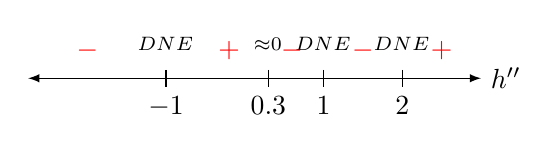
\begin{tikzpicture}
\draw[latex-latex] (-2.75,0) -- (3,0) node[right] {$h''$} ; %edit here for the axis
%\draw [very thick, - latex, blue] (0,0) -- (2.5,0);
%\node[circle,draw=blue, fill=blue, inner sep=0pt,minimum size=5pt] (a) at (0,0) {};
\foreach \x in  { -1,0.3, 1, 2} % edit here for the vertical lines
\draw[shift={(\x,0)},color=black] (0pt,3pt) -- (0pt,-3pt);
\foreach \x in  {-1, 0.3, 1,2}  % edit here for the numbers
\draw[shift={(\x,0)},color=black] (0pt,0pt) -- (0pt,-3pt) node[below] {$\x$};
\foreach \x in  {0.3}  % edit here for 0's
\draw[shift={(\x,3pt)}] node[above] {$^{\approx0}$};
\foreach \x in  {-1, 1, 2}  % edit here for DNE's
\draw[shift={(\x,3pt)}] node[above] {$^\text{DNE}$};
\foreach \x in  {-0.2, 2.5}  % edit here for +'s
\draw[shift={(\x,3pt)},color=red] node[above] {$+$};
\foreach \x in  {-2, 0.6, 1.5}  % edit here for -'s
\draw[shift={(\x,3pt)},color=red] node[above] {$-$};
\end{tikzpicture}
\end{center}

Hence we see that $h(x)$ is concave down on $(-\infty,-1)$ and $(0.32748,2)$, and is concave up on $(-1,0.32748)$ and $(2,\infty)$. Thus $h(x)$ has an inflection point at $x\approx 0.32748$ where 
$$y\approx h(0.32748) = \frac{2(0.32748-1)(0.32748+2)}{(0.32748+1)(0.32748-2)} \approx 1.41001.$$
There cannot be inflection points at $x=-1$ and $x=2$ because they are not in the domain of the function. 

Note that $h''(0.32748)\approx 9.58\times 10^{-9}$ is not zero, so the inflection point is not at $x=0.32748$. However, it is very close.


\end{enumerate}

We first plot all of the key points and features found:
\begin{itemize}
\item \textbf{Intercepts} $y$-intercept $(0,2)$ and $x$-intercept $(-2,0)$. 
\item \textbf{Asymptotes and/or Holes} Vertical asymptotes at $x=-1$ and $x=2$. A hole at $(1,0)$. Horizontal asymptote at $y=2$ to the right and left. 
\item \textbf{Local extrema} There are none. 
\item \textbf{Inflection points} Approximately $(0.32748,  1.41001)$
\end{itemize}

\begin{center}
\includegraphics[width=3in]{4-7Example3KeyPoints.png}
\end{center}

We can see that there are no key points to the right of the vertical asymptote at $x=2$, which may make it harder for us to "connect the dots" without any dots. There is nothing stopping us from plotting an extra point (or several). For instance, we can easily find
$$h(3) = \frac{2(2)^2(5)}{(2)(4)(1)} = 5$$
and add the point $(3,5)$ to our plot:

\begin{center}
\includegraphics[width=3in]{4-7Example3KeyPoints2.png}
\end{center}

Recall that $h(x)$ is decreasing everywhere on its domain. Recalling the concavity, we summarize the shape of $h(x)$ from left to right on the graph between all of the key features:
\begin{itemize}
\item $h(x)$ is decreasing and concave down on $(-\infty,-1)$, which fits between the horizontal asymptote to the left and the vertical asymptote at $x=-1$, passing through the $x$-axis at the point $(-2,0)$. 
\item $h(x)$ is decreasing and concave up from the vertical asymptote at $x=-1$ through the $y$-intercept at $(0,2)$, up until the inflection point at approximately $(0.32748,  1.41001)$. 
\item $h(x)$ is decreasing and concave down from the inflection point at $(0.32748,  1.41001)$ through the hole at $(1,0)$ and leading up to the vertical asymptote at $x=2$. 
\item $h(x)$ is decreasing and concave up from the vertical asymptote at $x=2$ to the far right edge of the graph, which fits with the horizontal asymptote to the right of the graph at $y=2$. 
\end{itemize}

In particular, note that the precise behavior of the vertical asymptotes we calculated matches the first-derivative information that the graph must be decreasing for all $x$-values. 

The remainder of the graph of $h(x)$ is filled in as shown below:


\begin{center}
\includegraphics[width=5in]{4-7Example3Graph.png}
\end{center}


\end{example}




\subsection*{Summary}
The following method was introduced in this section: 
\begin{quotation}
Curve Sketching Summary
\end{quotation}

\textbf{Key ideas:} In order to graph a rational function by hand, we determine the domain, intercepts, symmetry, vertical asymptotes and holes, end-behavior, and first- and second-derivative information for the function. We plot key points (intercepts, asymptotes, holes, local extrema, inflection points), summarize the behavior of the graph between each feature (increasing/decreasing, concave up/down), and then connect the points using the four possible shapes of nonlinear functions. 

\textbf{Other ideas reinforced/introduced:}  A polynomial function must have a local minimum or maximum between each of its $x$-intercepts. Using only information about the first and second derivative of a function, we can still get a remarkably accurate graph without knowing any precise $y$-values. Rational functions have vertical asymptotes and/or holes at points where they are undefined, depending on how the function cancels while taking the limit. Rational functions may also have horizontal asymptotes. 





\begin{center}
\textcolor{ocre}{\fbox{\fbox{\Large \bf \sc End of Section 4.7}}}
\end{center}

\hspace{-.5in}\rule{1.1\textwidth}{2pt}
























%----------------------------------------------------------------------------------------
%	PART
%----------------------------------------------------------------------------------------

\part{Spring Semester}

%----------------------------------------------------------------------------------------
%	CHAPTER 5 CONTENT
%----------------------------------------------------------------------------------------



\chapterimage{chapter5image1.jpg} % Chapter heading image
%image from https://www.sciencealert.com/known-universe-in-one-single-image-logarithmic-artwork-pablo-carlos-budassi
\chapterspaceabove{7.5cm} % Default whitespace from the top of the page to the chapter title on chapter pages
\chapterspacebelow{7cm} % Default amount of vertical whitespace from the top margin to the start of the text on chapter pages

%https://static9.depositphotos.com/1010826/1179/v/600/depositphotos_11791918-stock-illustration-tower-cranes.jpg

\chapter{Calculus with Exponential and Logarithmic Functions}


%----------------------------------------------------------------------------------------
%	Section 1
%----------------------------------------------------------------------------------------


\section{Inverse Functions}\label{sec:inversefunctions}


\subsection*{Learning Goals}

\begin{itemize}
	\item Understand the inverse of a function as reversing the process of the function, both intuitively and algebraically. 
	\item Identify algebraic and visual conditions under which a function does or does not have an inverse. 
	\item Summarize key properties of inverse functions and apply these to calculate and visualize inverses. 
\end{itemize}


\subsection{Why Inverse Functions?}

In order to study several categories of transcendental functions, you first need to know about inverse functions. Intuitively, an inverse function is a function that "undoes" another function. In this section we will first review some relevant properties of functions, define what it means to "undo" or  "invert" a function, determine conditions under which we \textit{can} invert a function, and then summarize some useful properties of inverse functions. 


\subsection{Brief Review of Functions}

Before discussing inverse functions, let's recall the basic definitions and terminology for functions from the beginning of the year: 

A {\bf function} $f$ from a set $A$ to a set $B$ is a rule $f$ that associates to each element $x$ of the {\bf domain} set $A$ exactly one element $y=f(x)$ of the {\bf range} set $B$. We will use the notation 
$$f: A\rightarrow B$$
to represent a function $f$ together with its domain set $A$ and range set $B$. This notation is pronounced "$f$ from $A$ to $B$." If $x$ and $y$ are variables that represent elements of the sets $A$ and $B$, respectively, then we say that $y$ is a function of $x$ and write $y=f(x)$. The variable $x$ is called the \textit{independent variable} and represents the "input" of the function. The function $f$ sends each input $x$ to \underline{one and only one} "output," some value of the \textit{dependent variable} $y$. Notice that $y$ depends on $x$, according to the assignment defined by the function $f$. 

\begin{example}
%https://activecalculus.org/prelude/sec-changing-inverse.html 
%MODIFY
%
%Function from APC Preview Activity 1.7.1 broken down to illustrate the above definitions. Verbal descriptions of domain and range, and an example of elements of each that map to each other, but do not give domain and range as sets. Note that I'm conflating codomain and range. This is intentional. I won't ever mention codomain. 

The rule $F=g(C)=\frac{9}{5}C+32$ is the function that takes Celsius temperature inputs $C$ and produces the corresponding Fahrenheit temperature outputs $F$.

Therefore, the domain of $g$ is all possible Celsius temperatures, and the range of $g$ is all possible Fahrenheit temperatures.  If we know that the temperature is 25 degrees Celsius, but want to know the corresponding Fahrenheit temperature, we can compute $g(25)=\frac{9}{5}(25)+32=77$ degrees Fahrenheit.
\end{example}

Recall that the graph of a function must pass the \textit{vertical line test} (Theorem \autoref{thm:vlt}):

\begin{quotation}
\textbf{The Vertical Line Test:} 
A graph represents a function if and only if every vertical line intersects the graph in at most one point. 
\end{quotation}

\begin{example}
%THE GRAPH OF THE FUNCTION FROM APC PREVIEW ACTIVITY 1.7.1 WITH A FEW DASHED VERTICAL LINES.
The following is the graph of the function $F=g(C)=\frac{9}{5}C+32$.  We can see that every vertical line intersects the graph in at most one point, so this graph represents a function, because it passes the vertical line test.

\begin{center}
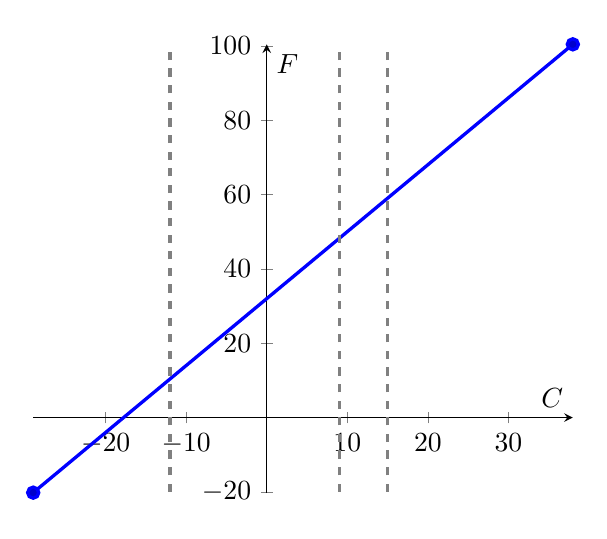
\begin{tikzpicture}[>=latex]
    \begin{axis}[
%width=6cm,
	axis lines=middle,
	xlabel=\(C\), ylabel=\(F\),
	every axis plot/.style={very thick},
                ]
    \addplot coordinates { (38,100.4) (-29,-20.2)};
    \addplot[gray, dashed] coordinates { (9,-20) (9,100.4)};
       \addplot[gray, dashed] coordinates { (-12,-20) (-12,100.4)};
            \addplot[gray, dashed] coordinates { (15,-20) (15,100.4)};
	\end{axis}
    \end{tikzpicture}
\end{center} 
\end{example}


\subsection{Defining Inverse Functions}

%From APC 1.7 intro:
Because every function is a process that converts a collection of inputs to a corresponding collection of outputs, a natural question is: for a particular function, can we \textit{change perspective and think of the original function's outputs as the inputs for a reverse process}? If we phrase this question algebraically, it is analogous to asking: given an equation that defines $y$ as a function of $x$, is it possible to find a corresponding equation where $x$ is a function of $y$?


\begin{example}\label{ex:Preview1-7-1}
  It is possible to solve the equation $F=\frac{9}{5}C+32$ for $C$. In other words, we are able to isolate $C$ through a series of algebraic steps. Doing so results in the equation which takes Fahrenheit temperature inputs $F$ and produces the corresponding Celsius temperature outputs $C$, meaning a function $C=h(F)$.

We start with the equation 
\[
F=\frac{9}{5}C+32
\]
and subtract $32$ from both sides, to get
\[
F-32=\frac{9}{5}C.
\]
Then to get $C$ by itself, we multiply both sides by $\frac{5}{9}$ to get 
\[
C=\frac{5}{9}(F-32).
\]

Note that the equation $C=\frac{5}{9}(F-32)$ expresses $C$ as a function of $F$.  Call this function $h$ so that $C=h(F)=\frac{5}{9}(F-32)$. 

Now, $g$ is a function which takes a temperature in degrees Celsius, and converts it to a temperature in degrees Fahrenheit, and $h$ is a function which takes a temperature in degrees Fahrenheit, and converts it to a temperature in degrees Celsius.  

Take a moment to think about what would happen if we convert from one system to the other and then back. In other words, what happens if we compose these functions? Lets find the simplest expression that we can for the composite function $j(C)=h(g(C))$.

\[
\begin{split}
j(C)&=h(g(C))\\
&=\frac{5}{9}(g(C)-32)\\
&=\frac{5}{9}\left(\frac{9}{5}C+32-32\right)\\
&=\frac{5}{9}\left(\frac{9}{5}C\right)\\
&=C.
\end{split}
\]

Next, we find the simplest expression that we can for the composite function $k(F)=g(h(F))$:

\[
\begin{split}
k(F)&=g(h(F))\\
&=\frac{9}{5}h(F)+32\\
&=\frac{9}{5}\left(\frac{5}{9}(F-32)\right)+32\\
&=(F-32)+32\\
&=F.
\end{split}
\]

Notice how simple both of these compositions become! This is not a coincidence\ldots

%Why are these functions so simple?  Let's think about how the functions $g$ and $h$ process inputs to generate outputs and what happens when we first execute one followed by the other. The composite function $g(h(F))$ takes a temperature in Fahrenheit, converts it to Celsius, and then converts it to Fahrenheit.  Since this should be the same as the original temperature in Fahrenheit, it makes sense that $g(h(F))=F.$  Similarly, the composite function $h(G(C)$ takes a temperature in Celsius, converts it to Fahrenheit, and then converts it to back to Celsius. 
\end{example}

\textbf{Inverses Reverse Each Other!} In Example \ref{ex:Preview1-7-1}, we found that for the function $F=g(C)=\frac{9}{5}C+32$,  it's  possible to solve for $C$ in terms of $F$ and write $C=h(F) = \frac{5}{9}(C-32)$.  The first function, $g$, converts Celsius temperatures to Fahrenheit ones; the second function, $h$, converts Fahrenheit temperatures to Celsius ones. Thus, the process $h$ \textit{reverses the process} of $g$,  and likewise the process of $g$ \textit{reverses the process} of $h$.  This is also why it makes sense that $j=h\circ g$ and $k = g\circ h$ are so simple, namely that $j(C) = h(g(C)) = C$ and $k(F) = g(h(F)) = F$, meaning both compositions end up back where they started. If, for instance, we take a Celsius temperature $C$,  convert it to Fahrenheit, and convert the result back to Celsius, we arrive back at the Celsius temperature we started with: $h(g(C)) = C$. 

Similar work is sometimes possible with other functions. When we can find a new function that reverses the process of the original function, we say that the original function "has an inverse function" and make the following formal definition.

\begin{definition}[The Inverse of a Function]\label{def:inverses}
Let $f:A\to B$ be a function.  If there exists a function $g: B\to A$ such that 
$$g(f(a))=a \textrm{  and  }f(g(b))=b$$
for each $a$ in $A$ and each $b$ in $B$, then we say that $f$ has an {\bf inverse function} and that the function $g$ is {\bf the inverse of $f$}.\\

\noindent
A function is called {\bf invertible} if it has in inverse function. \\

\noindent
\textbf{Notation:} When a given function $f$ has a corresponding inverse function $g$, we usually rename $g$ as $f^{-1}$ which we read aloud as ``$f$-inverse". The equation $g(f(a))=a$ now reads $$f^{-1}\big(f(a)\big)=a,$$ which we interpret as saying ``$f$-inverse converts $f(a)$ back to $a$. We similarly write that $$f\big(f^{-1}(b)\big)=b.$$
\end{definition}

Note particularly what the equation $g(f(a))=a$ says: for any input $a$ in the domain of $f$. the function $g$ will reverse the process of $f$ (which converts $a$ to $f(a)$) because $g$ converts $f(a)$ back to $a$.  



%From Taalman Section 0.6
Note that the two conditions in Definition \ref{def:inverses} guarantee that if a function $g$ is the inverse of a function $f$, then $f$ is the inverse of the function $g$. 

\begin{example}\label{ex:invertingxcubed}
%EXAMPLE FROM MIDDLE OF PAGE 67 OF TAALMAN

For example, the functions $f(x) = x^3$ and $g(x) = \sqrt[3]{x}$ are inverses of each other. Intuitively, taking the cube of a number is undone by taking the cube root, and vice versa.  Its easy to verify this algebraically by converting $\sqrt[3]{x} = x^{1/3}$:

$$g(f(x))=\sqrt[3]{x^3}=(x^3)^{1/3} = x^{3\cdot(1/3)} = x^1 = x, \textrm{ and}$$
$$f(g(x))=(\sqrt[3]{x})^3=(x^{1/3})^3 = x^{(1/3)\cdot 3} = x^1=x.$$
Thus we can write $f^{-1}(x) = \sqrt[3]{x}$ for the inverse of $f(x) = x^3$. Likewise, we can write $g^{-1}(x) = x^3$ for the inverse of $g(x) = \sqrt[3]{x}$. 

%AND CONTINUE THROUGH THE END OF BOTH COMPOSITIONS. 
\end{example}


\noindent
\fbox{\parbox{6in}{
\textbf{Very Important!}
It is  critical to note that although we use the notation $x^{-1}$ to denote the reciprocal $\frac{1}{x}$ of a number or variable $x$, the notation $f^{-1}$ does {\em not} stand for the reciprocal $\frac{1}{f}$.  The notation $f^{-1}$ stands for $f$-inverse!  We are now using the same notation for two very different concepts, but it should be clear from the context what we mean.
}}




\begin{exercise}\label{ex:dolbearinverse}
%ACTIVITY 1.7.2 FROM APC
Recall Dolbear's function $F=D(N)=40+\frac{1}{4}N$ that converts the number, $N$, of snowy tree cricket chirps per minute to a corresponding Fahrenheit temperature $F$. %We established in Section \ref{subsec:modeling} that the domain of $D$ is $[40,180]$ and the range of $D$ is $[50,85]$.
\begin{enumerate}[label=\alph*.,itemsep=5pt]
\item Solve the equation $F=40+\frac{1}{4}N$ for $N$ in terms of $F$. Call the resulting function $N=E(F)$. 
%\begin{solution}
%We start with the equation 
%\[
%F=40+\frac{1}{4}N
%\]
%and subtract $40$ from both sides, to get
%\[
%F-40=\frac{1}{4}N.
%\]
%Then to get $N$ by itself, we multiply both sides by $4$ to get 
%\[
%N=4(F-40).
%\]
%\end{solution}

\item Explain in words the process or effect of the function $N=E(F)$. What does it take as input? What does it generate as output?
%\begin{solution}
%The function $N=E(F)$ takes as its input a Fahrenheit temperature, and produces as its output, a number of snowy tree cricket chirps per minute.
%\end{solution}

\item Use the function $E$ that you found in (a) to compute $j(N)=E(D(N))$. Simplify your result as much as possible. Do likewise for $k(F)=D(E(F))$.What do you notice about these two composite functions $j$ and $k$? Compare this result to Definition \ref{def:inverses}.
%\begin{solution}
%\[
%\begin{split}
%j(N)&=E(D(N))\\
%&=4(D(N)-40)\\
%&=4\left(40+\frac{1}{4}N-40\right)\\
%&=4\left(\frac{1}{4}N\right)\\
%&=N.
%\end{split}
%\]
%
%\[
%\begin{split}
%k(F)&=D(E(F))\\
%&=40+\frac{1}{4}E(F)\\
%&=40+\frac{1}{4}(4(F-40))\\
%&=40+(F-40)\\
%&=F.
%\end{split}
%\]
%
%Both $j(N)$ and $k(F)$ are functions which give, as their output, whatever is given as the input.
%\end{solution}

\item Do the functions $F=D(N)$ and $N=E(F)$ express different relationships between $F$ and $N$ or do they express the same relationship in two different ways? Explain.
%\begin{solution}
%Since we are able to use algebra to get from one equation to another, these equations express the same relationship between $F$ and $N$.  The first allows one to compute a temperature given a number of chirps per minute, and the second allows one to compute a number of chirps per min from a temperature.
%\end{solution}

  \end{enumerate}

\end{exercise}





%AND EXPOSITION FOLLOWING ABOUT TWO PERSPECTIVES WITH THE BOX AS A REMARK

%\todo{Use variables x and y instead of y and t, and also show algebra reversing the relationship}
When a given function has an inverse function, it allows us to express the same relationship from two different points of view. 

\begin{example} 
For instance, if $w=f(z) = 2z+1$, we can show that the function $z=g(w)=\dfrac{w-1}{2}$ reverses the effect of $f$ (and vice versa), and thus $g=f^{-1}$.  We observe that

$$\begin{aligned}
w&= 2z+1\\
w-1 &= 2z\\
\frac{w-1}{2} &= z
\end{aligned}$$
so that 
$$w=f(z)=2z+1\qquad \textrm{ and }\qquad z=f^{-1}(w)=\dfrac{w-1}{2}$$
are equivalent forms of the same equation, and thus they say the same thing from two different perspectives. The first version of the equation is solved for $w$ in terms of $z$, while the second equation is solved for $z$ in terms of $w$.  
\end{example}


This important principle holds in general whenever a function has an inverse function:
 
\noindent
\fbox{\parbox{6in}{
\textbf{Two perspectives from a function and its inverse function.}  If $y=f(x)$ has an inverse function, then the equations
 
 $$y=f(x)\qquad \textrm{ and }\qquad x=f^{-1}(y)$$
 
 say the exact same thing but from two different perspectives.
}}
 
 
 \begin{example}
Suppose $f$ is an invertible function with inverse $f^{-1}$. If $f(3) = 7$, what does this tell us about $f^{-1}$?

The function $f^{-1}$ reverses the process of $f$, so that inputs become outputs and vice versa. Thus if $f$ takes the input of 3 to the output of 7:
$$f(3)=7$$
then $f^{-1}$ should reverse this process and take the input of 7 to the output of 3:
$$f^{-1}(7)=3.$$

Thus know that $f^{-1}(7) = 3$. 

We check this against Definition \ref{def:inverses} to make sure our line of reasoning is correct:
$$f^{-1}(f(3)) = f^{-1}(7)=3$$
and 
$$f(f^{-1}(7)) = f(3) = 7$$
as desired. 
\end{example}




\begin{example}
The number $N$ of operating drive-in movie theaters in the state of Virginia in various years $y$ is given in the table below. We can view $N$ as a function of $y$ and write $N=f(y)$. 

\begin{table}[H]
\centering
\begin{tabular}{|l|r|r|r|r|r|r|}
\hline
$y$ & 1958 &1967 & 1972 & 1977 & 1982 & 1999\\
\hline
$N$ & 143 & 109 & 102 & 87 & 56 & 9\\
\hline
\end{tabular}
\caption{$N=f(y)$ gives the number $N$ of operating drive-in movie theaters in the year $y$.}
\end{table}

Recall that tables are a convenient way of summarizing corresponding inputs and outputs of a function. For instance, we know that $f(1977)=87$, meaning that in 1977, there were 87 operating drive-in movie theaters. On the other hand, given the data available, it is accurate to say that when there were 87 operating movie theaters, the year was 1977. In terms of functions, we can write $f^{-1}(87) = 1977$. Is this saying anything meaningfully different? No. Remember: inverse functions are just a change in perspective. 

We can summarize the values of this inverse perspective in the table below simply by swapping the rows:

\begin{table}[H]
\centering
\begin{tabular}{|l|r|r|r|r|r|r|}
\hline
$N$ & 143 & 109 & 102 & 87 & 56 & 9\\
\hline
$y$ & 1958 &1967 & 1972 & 1977 & 1982 & 1999\\
\hline
\end{tabular}
\caption{The year $y$ when there were $N$ operating drive-in movie theaters.}
\end{table}

This table defines $y$ as a function of $N$, and we can write $y=f^{-1}(N)$. Lastly, we will finish by reorganizing the table so that our "input" values of $N$ appear in increasing order, as is typical (though not strictly necessary):

\begin{table}[H]
\centering
\begin{tabular}{|l|r|r|r|r|r|r|}
\hline
$N$ & 9 & 56 & 87 & 102 & 109 & 143\\
\hline
$y$  & 1999& 1982 &1977 & 1972 & 1967 & 1958\\
\hline
\end{tabular}
\caption{A table of values for $y=f^{-1}(N)$.}
\end{table}


\end{example}


\begin{remark}
Notice that we sometimes swap the input and output variables while finding the inverse function (as in Example \autoref{ex:invertingxcubed}), while sometimes we do not swap variables (as in Exercise \ref{ex:dolbearinverse}). It is only appropriate to switch input and output variable for functions that are entirely abstract, and especially if we are talking about the inverse as its own function and want to graph it on the same set of axes as the original function. In cases where the variables represent real-world quantities, such as number of cricket chirps and temperature, it would not make sense to switch variables.  
\end{remark}


\begin{exercise}
In your own words, explain the meaning and purpose of an inverse function. 
\end{exercise}


\subsection{When is a Function Invertible?}

Not all functions have inverses. 


%Taalman Section 0.6
\begin{example}\label{ex:nonHLT}
For example, consider the squaring function $f(x) = x^2$ with the domain $\mathbb{R}$. How could we reverse the process defined by $f$? 

Observe that $f(2) = 4$ and $f(-2)=4$.  An inverse of $f$ would have to send the input 4 back to both $2$ and $-2$ in order to reverse $f$. This violates our rules for a function since an input must have one and only one output. Thus $f(x) = x^2$ does \textit{not} have an inverse. 

In particular, $\sqrt{x^2} = x$ is \textit{not} always true, so that $\sqrt{x}$ is \textit{not} a true inverse to $x^2$. \textit{Why not? Find a value for $x$ such that $\sqrt{x^2}\neq x$.}
\end{example}

It's important to note in Definition \ref{def:inverses} that we say "\textit{If} there exists\ldots." That is, we are not guaranteed that an inverse function exists for a given function. Thus, we might ask: how can we determine whether or not a given function has a corresponding inverse function? As with many questions about functions, there are often three different possible ways to explore such a question: through a table, through a graph, or through an algebraic formula.




%APC 1.7

\begin{example}
%\todo{EXAMPLE 1.7.2 FROM APC, REPHRASED SO NOT ASKED AS A QUESTION, AND USE FUNCTION NAMES G (INSTEAD OF F) AND H (INSTEAD OF G). Maybe explicitly give the tabular forms of the inverse relationships as well for emphasis and observe that g is not a function. }
%\robyn{ Ive filled this out, but i am not exactly sure what you want for this last part, so I'm leaving this comment here for you to check!}

Let $g$ and $h$ be functions defined by the following tables:
\begin{table}[H]
    \begin{subtable}{.5\linewidth}
      \centering
         \begin{tabular}{c c c c c c}
\toprule
$x$ &0 & 1 & 2 & 3 & 4 \\
\midrule
$g(x)$ & 6 & 4 & 3 & 4 & 6 \\
\bottomrule
\end{tabular}
        \caption{A table defining $g$.}
        \label{tab:notinvertible}
    \end{subtable}%
    \begin{subtable}{.5\linewidth}\label{table1.7.4}
      \centering
  \begin{tabular}{c c c c c c}
\toprule
$x$ &0 & 1 & 2 & 3 & 4 \\
\midrule
$h(x)$ & 3 & 1 & 4 & 2 & 0 \\
\bottomrule
\end{tabular}
        \caption{A table defining $h$.}
        \label{tab:invertible}
    \end{subtable} 
        \caption{Tables defining $g$ and $h$}
\end{table}

The function $g$ does not have an inverse function because there are two different inputs that lead to the same output:  $g(0)=6$ and  $g(4)=6$. If we attempt to reverse this process, we have a situation where the input $6$ would correspond to two potential outputs, $0$ and $4$. 

Note that if we try to reverse the rows of  \autoref{tab:notinvertible},  we can see the "input" of 6 occurs twice in the top row and has two different "outputs." 
 \begin{table}[H]
      \centering
         \begin{tabular}{c c c c c c}
\toprule
$x$ (formerly $g(x)$) & 6 & 4 & 3 & 4 & 6 \\
\midrule
$g^{-1}(x)$ (formerly $x$) &0 & 1 & 2 & 3 & 4 \\
\bottomrule
\end{tabular}
    \caption{A table attempting to define $g^{-1}$ by swapping the rows of \autoref{tab:notinvertible}. This is not a function.}
\end{table}


However, the function $h$ does have an inverse function because if we reverse the rows in Table (b), each input  indeed corresponds to one and only one output:

\begin{table}[H]
\centering
  \begin{tabular}{c c c c c c}
\toprule
$x$ (formerly $h(x)$) & 3 & 1 & 4 & 2 & 0 \\
\midrule
$h^{-1}(x)$ (formerly $x$) &0 & 1 & 2 & 3 & 4 \\
\bottomrule
\end{tabular}
    \caption{Table defining $h^{-1}$ by swapping the rows of \autoref{tab:invertible}}
\end{table}

 We can thus make observations such as $h^{-1}(4)=2$, which is the same as saying that $h(2)=4$, just from a different perspective.
 
 If we "clean up" the table for $h^{-1}$ by putting its inputs in order, it looks like what we would expect to see in a table defining a function:
 
 \begin{table}[H]
\centering
  \begin{tabular}{c c c c c c}
\toprule
$x$  &0 & 1 & 2 & 3 & 4 \\
\midrule
$h^{-1}(x)$  &4 & 1 & 3 & 0 & 2 \\
\bottomrule
\end{tabular}
    \caption{Table defining $h^{-1}$}
\end{table}
 
 
\end{example}

In the above two examples, we see that  if we can identify at least one pair of distinct inputs that lead to the same output (such as $f(2)=f(-2)=4$ or $g(0)=g(4)=6$), then the process of the function cannot be reversed and the function does not have an inverse.

\begin{example}\label{ex:HLT}
%EXAMPLE 1.7.5 FROM APC BUT REPHRASED WITHOUT THE QUESTION. ALSO SHORTEN SOLUTION. REFER TO VLT BUT ASSUME STUDENTS KNOW HOW TO READ GRAPHS (SO CUT MOST OF FIRST PARAGRAPH). 
Consider the functions $p$ and $q$, defined by the graphs below:

\begin{figure}[H]
     \centering
     \begin{subfigure}[b]{0.4\textwidth}
         \centering
         \includegraphics[width=\textwidth]{ACFigure1-7-7.png}
         \caption{The graph that defines function $p$}
         \label{}
     \end{subfigure}
     \hfill
     \begin{subfigure}[b]{0.4\textwidth}
         \centering
         \includegraphics[width=\textwidth]{ACFigure1-7-6.png}
         \caption{The graph that defines function $q$}
         \label{}
     \end{subfigure}

\end{figure}

We note explicitly that  $p$ is a function because its graph passes the Vertical Line Test.  If we attempt to change perspective and use the graph of $p$ to view $x$ as a function of $y$, we see that this fails because the $y$-value $c$ is associated with two different $x$-values,  $a$ and $b$.  Said differently, because the horizontal line $y=c$ intersects the graph of $p$ at both $(a,c)$ and $(b,c)$, we cannot view $y$ as the input to a function process that produces the corresponding $x$-value. If we turn our head to the side and view the $y$-axis as our inputs, the graph would not pass this tipped over Vertical Line Test. Therefore, $p$ does not have an inverse function.

On the other hand, the function $q$ does have an inverse because we can view $x$ as a function of $y$ via the graph (provided that the behavior seen in the figure continues). This is because for any choice of $y$, there corresponds one and only one $x$ that results from $y$.  We can think of this visually by starting at a value such as $y=c$ on the $y$-axis, moving horizontally to where the line intersects the graph of $p$ and then moving down to the corresponding location (here $x=a$) on the horizontal axis. From the behavior of the graph of $q$ (a straight line that is always increasing), we see that this correspondence will hold for any choice of $y$, and thus indeed $x$ is a function of  $y$.  From this, we can say that $q$ indeed has an inverse function. We thus can write that $q^{-1}(c)=a$, which is a different way to express the equivalent fact that $q(a)=c$. Likewise, we can see that $q^{-1}(d) = b$, since $q(b) = d$. 

\end{example}


What have we observed so far? Functions are invertible provided that no two inputs produce the same output. Visually, no two points can be at the same height on the graph, so that no horizontal line intersects the graph in more than one point. The graphical observations that we made for the function $q$ in Example \ref{ex:HLT} provide a general test for whether or not a function given by a graph has a corresponding inverse function.

\begin{theorem}[Horizontal Line Test]\label{thm:HLT}
A function whose graph lies in the $xy$-plane has a corresponding inverse function if and only if every horizontal line intersects the graph at most once. When the graph passes this test, the horizontal coordinate of each point on the graph can be viewed as a function of the vertical coordinate of the point.
\end{theorem}


\begin{definition}[One-to-One]
A function $f$ whose graph passes the horizontal line test is said to be {\bf one-to-one}. This is because the inputs and outputs of such a function pair uniquely with each other, without any "doubling up" of multiple inputs to one output. \\

\noindent
Another way of stating that a function is one-to-one is that, for any values $a$ and $b$ of the independent variable, 
\begin{quotation}if $a\neq b$, then $f(a)\neq f(b)$. 
\end{quotation}

\noindent
Equivalently, using the contrapositive, we can phrase this as
\begin{quotation} if $f(a)=f(b)$, then $a=b$. \end{quotation}
\end{definition}



\begin{exercise}
Give an example from your own life or experience of a function that is invertible, a.k.a one-to-one. \textit{Recall that this means that each value of the dependent variable corresponds to only one value of the independent variable. In other words, the function cannot repeat output values.}
\end{exercise}


\begin{example}[Identifying An Invertible Function Visually]\label{ex:visualinvertible1}
%R(T) OF EXAMPLE 1.7.8 OF APC. PICTURE FIRST AND THEN ALGEBRAICALLY FINDING THE INVERSE. INCLUDE 1-1 TERMINOLOGY.
Consider the function $y=r(t)=3-\dfrac{1}{5}(t-1)^3$ defined by the graph below:

\begin{figure}[H]
     \centering

         \includegraphics[width=.3\textwidth]{ACFigure1-7-9-r.png}
         \caption{The graph that defines function $r$}
         \label{}
\end{figure}

We can see that $r(t)$ passes the horizontal line test, and is therefore one-to-one.  This means that each point on the graph can be viewed as a function of the vertical coordinate of the point, and therefore $r(t)$ has an inverse function. 
\end{example}

\begin{example}[Finding the Inverse of an Invertible Function Algebraically] Thanks to Example \autoref{ex:visualinvertible1}, we know that $y=r(t)=3-\dfrac{1}{5}(t-1)^3$ is invertible, meaning that the inverse function $t=r^{-1}(y)$ exists. To find an explicit formula for this function, we take the equation $y=3-\dfrac{1}{5}(t-1)^3$, and solve for $t$:

First, subtract $3$ from both sides to get

$$y-3=-\dfrac{1}{5}(t-1)^3.$$

Next, multiplying both sides by  $-5$, it follows that

$$-5(y-3)=(t-1)^3.$$

Because the cube root function has the property that $\sqrt[3]{z^3}=z$ for every real number $z$ (since the cube root function is the inverse function for the cubing function, and each function has both a domain and range of all real numbers), we can take the cube root of both sides of the preceding equation to get

$$\sqrt[3]{-5(y-3)}=t-1.$$

Finally, adding 1 to both sides, we have determined that
  
  $$t=1+\sqrt[3]{-5(y-3)}.$$
 
Because we have been able to express $t$ as a single function of $y$ for every possible value of $y$, this shows that $r$ indeed has an inverse and that $t=r^{-1}(y)=1+\sqrt[3]{-5(y-3)}$.
 
\end{example}

\begin{example}[Visually and Algebraically NOT Invertible]
%S(T) OF EXAMPLE 1.7.8 OF APC. PICTURE FIRST AND THEN SHOWING ALGEBRAICALLY WHAT GOES WRONG WHEN TRYING TO FIND THE INVERSE. INCLUDE 1-1 TERMINOLOGY AND AN EXPLICIT EXAMPLE OF AN A AND B THAT MAP TO THE SAME VALUE. 

Consider the function $y=s(t)=3-\dfrac{1}{5}(t-1)^2$ defined by the graph below:

\begin{figure}[H]
     \centering

         \includegraphics[width=.3\textwidth]{ACFigure1-7-10-s.png}
         \caption{The graph that defines function $s$}
         \label{}
\end{figure}


We can see that $s(t)$ does NOT pass the horizontal line test; in particular, it looks like $s(2)=s(0)$, and using the formula $s(t) = 3-\frac{1}{5}(t-1)^2$, we can indeed calculate that $s(2)=s(0)=\dfrac{14}{5}$.  Therefore $s(t)$ does not have an inverse function. \\

What if we did not have a picture? Would we still be able to determine that $y=s(t)$ is not invertible? 
If we were to try to solve for $t$ in terms of $y$ algebraically, we could again subtract $3$ from both sides to get
$$y-3=-\dfrac{1}{5}(t-1)^2.$$

Next, multiplying both sides by  $-5$, it follows that

$$-5(y-3)=(t-1)^2.$$

Here, however, we encounter a crucial issue. Recall from Example \ref{ex:nonHLT} that the function  $f(x)=x^2$ does not have an inverse. It takes any nonzero number and its opposite to the same output (e.g.  $(-5)^2=25=(5)^2$), this means that we have to account for both possible inputs that result in the same output. Based on our last equation, this means that either

$$t-1=\sqrt{-5(y-3)}\qquad\textrm{ or }\qquad t-1=-\sqrt{-5(y-3)}.$$

As such, we find not a single equation that expresses  $t$ as a function of $y$, but rather two:

$$t=1+\sqrt{-5(y-3)}\qquad\textrm{ or }\qquad t=1-\sqrt{-5(y-3)}.$$

It appears that $t$ cannot be expressed as a single function of $y$; and indeed, $y=s(t)=3-\dfrac{1}{5}(t-1)^2$ does not have an inverse function.


\end{example}



\begin{exercise}
%\todo{APC ACTIVITY 1.7.3 BUT NOT ALL PARTS. I THINK PARTS B, D, AND E. WE CAN USE THE OTHER PARTS ON THE WORKSHEET FOR TODAY. INCLUDE 1-1 TERMINOLOGY AND ASK IF THE FUNCTION IS NOT 1-1, GIVE AN EXAMPLE OF TWO INPUTS WITH THE SAME OUTPUT. }
%
%\robyn{ lmk if this is what you were thinking? I also adjusted the worksheet problem with the other parts of this, so if you change the wording below, we should change it there too!}


Determine, with justification, whether each of the following functions is one-to-one, and therefore whether it has an inverse function. \textit{Remember, both of these are the same as saying that the graph passes the Horizontal Line Test (Theorem \autoref{thm:HLT}).}\\

\noindent
 For each function that is \textbf{not} one-to-one, give an example of two inputs with the same output, such as $f(1)=3$ and $f(2)=3$.  \\
 For each function that \textbf{is} one-to-one, give two examples of values of the inverse function by writing statements such as ``$f^{-1}(3)=1$".
 
 \begin{enumerate}[label=\textbf{\alph*.},itemsep=10pt,topsep=10pt]
%
%\item The function $f: S\to S$ given by the following table, where $S=\{0,1,2,3,4\}$.
%
%Table 1.7.11:
%\[
%\begin{array}{cccccc}
%x&0&1&2&3&4\\
%\hline
%f(x)&1&2&4&3&2\\
%\end{array}
%\]
%\begin{solution}
%%The function $f(x)$ does not have an inverse function, as such a function $f^{-1}$ would need to have $f^{-1}(2)=1$ and $f^{-1}(2)=4$.  Since it is not possible for a function to associate a single input to two different outputs, $f$ does not have an inverse.
%%\end{solution}

\item The function $g: S\to S$, given by the following table,  where $S=\{0,1,2,3,4\}$.

\[
\begin{array}{cccccc}
x&0&1&2&3&4\\
\hline
g(x)&4&0&3&1&2\\
\end{array}
\]
%\begin{solution}
%The function $g(x)$ does have an inverse, as each value $g(x)$ is associated to exactly one $x$ value.  $g^{-1}(0)=1$ and $g^{-1}(1)=3$
%\end{solution}

%\item The function $p$ given by $p(t)=7-\frac{3}{5}t$. Assume that the domain and codomain of $p$ are both ``all real numbers."
%\begin{solution}
%The function $p(t)$ describes a line, and a line passes the horizontal line test!  So $p(t)$ has and inverse.  $p^{-1}(7)=0$, and $p^{-1}(0)=\frac{35}{3}$.
%\end{solution}

\item The function $q$ given by $q(t)=7-\frac{3}{5}t^4$. Assume that the domain of $q$ is ``all real numbers."
%\begin{solution}
%You may graph this to see that $q(t)$ does not pass the horizontal line test, and doesn't have an inverse.  Or, notice that $q(1)=q(-1)=\frac{32}{5}$, so that any inverse would need to have $q^{-1}\left(\frac{32}{5}\right)=1$ and $-1$, which would fail to be a function.
%\end{solution}

\item The function $r$  given by the following graph: 


\begin{center}
         \includegraphics[width=2in]{ACFigure1-7-13.png}
         \end{center}


Assume that the graph shows all of the important behavior of the function and that the apparent trends continue beyond what is pictured.

%\begin{solution}
%Figure 1.7.13 passes the horizontal line test, we can see from the graph that $r^{-1}(0)=0$ and $r^{-1}(-2)=1$.  Figure 1.7.14 is does not pass the horizontal line test for $1<y<2$, so does not have an inverse.
%\end{solution}
\end{enumerate}

\end{exercise}


\subsection{Properties of Inverse Functions}

When a function has an inverse function, we have observed several important relationships that hold between the original function and the corresponding inverse function, which we summarize here. Note that many of these properties seem to be saying the same thing, only with a different emphasis. 

\begin{theorem}[Properties of an inverse function]\label{thm:inverseproperties}
Let $f:A\to B$ be a function whose domain is $A$ and whose range is $B$ be such that $f$ has an inverse function $f^{-1}$.  Then:

 \begin{enumerate}[label=\textbf{\alph*.},itemsep=15pt,topsep=10pt]
 \item The functions $f$ and $f^{-1}$ reverse one another's processes.  Symbolically, $f^{-1}(f(a))=a$ for every input $a$ in the domain of $f$, and similarly, $f(f^{-1}(b))=b$ for every input $b$ in the domain of $f^{-1}$.
 
 
 \item If $b=f(a)$, then we can express the exact same relationship from a different perspective by writing $a=f^{-1}(b)$.
 
\item The domain of $f^{-1}$ is $B$ and its range is $A$. Symbolically, $f^{-1}:B\to A$, meaning that $f^{-1}$ is a rule that assigns to each element $b$ of the set $B$ and element $a$ of the set $A$ via $a=f^{-1}(b)$. 


\item If a point $(a,b)$ lies on the graph of $f$, then we write $b=f(a)$.  From this, we can equivalently say that $a=f^{-1}(b)$.  Hence, the point $(b,a)$ lies on the graph of $a=f^{-1}(b)$. 

\item The graph of $y=f^{-1}(x)$ is the graph of $y=f(x)$ reflected across the line $y=x$. 
\end{enumerate}
\end{theorem}


Property (e) above is new but follows immediately from property (d): because inverse functions reverse inputs and outputs, inverting a function reverses the $x$- and $y$-values in the $xy$-plane. This means that the graph of the inverse of a function is a reflection of the graph of the original function across the line $y=x$. 

%From Taalman page 68

\begin{example}[Applying Properties and Visualizing Inverse Functions]
For example, consider the function $f(x) = \sqrt{x+1}$. $f(x)$ has the domain $[-1,\infty)$ since we need $x\geq -1$ in order to have $x+1\geq 0$. 

We can see from the graph below that $f(x)$ is invertible and one-to-one because it passes the horizontal line test. We can also observe from the graph that $f(x)$ appears to have the range $[0,\infty)$. 

%\todo{GRAPH OF F(X) FROM TAALMAN PAGE 68 (LEFT MOST PICTURE)}

\begin{figure}[h]
\centering
 \includegraphics[width=2in]{TaalmanPage68a.png}
 \caption{The graph of $f(x) = \sqrt{x+1}$ has domain $[-1,\infty)$ and range $[0,\infty)$.}
 \end{figure}


To find the inverse function $f^{-1}$, we reverse inputs and outputs, meaning we solve $y=\sqrt{x+1}$ for $x$:

$$\begin{aligned}
y&= \sqrt{x+1}\\
y^2 &= x+1\\
y^2-1&= x
\end{aligned}$$

Changing notation so that $x$ is again the independent variable, we see that the inverse of $f(x)$ is given by the formula $$f^{-1}(x)=x^2-1.$$

 \autoref{fig:TaalmanPage68b} illustrates Property (d) of Theorem \ref{thm:inverseproperties} for $f(x)=\sqrt{x+1}$: the graph of $f^{-1}(x)$ is the graph of $f(x)$ reflected across the line $y=x$:


\begin{figure}[H]
\centering
 \includegraphics[width=2.5in]{TaalmanPage68b.png}
 \caption{Reflect $f(x)$ across the line $y=x$ to obtain $f^{-1}(x)$.}
 \label{fig:TaalmanPage68b}
 \end{figure}
 
Note that $y=x^2-1$ is not invertible; if you graph this, you will get a parabola that does not pass the horizontal line test. This appears to contradict our previous calculations! However, the important detail here comes from Theorem \ref{thm:inverseproperties} part (c):

\begin{quotation}
The domain of $f^{-1}$ is $B$ and its range is $A$.
\end{quotation}

In this example, the range of $f(x)=\sqrt{x+1}$ was $[0,\infty)$ so that the domain of $f^{-1}(x)$ must be the same set $[0,\infty)$. We see this in  \autoref{fig:TaalmanPage68b} above: only the half of the parabola with $x\geq 0$ results from reflecting $f(x) = \sqrt{x+1}$ across the line $y=x$. Thus when we consider $f^{-1}(x)=x^2-1$ as the inverse of $f(x) = \sqrt{x+1}$, we must restrict the domain to $[0,\infty)$, as in  \autoref{fig:TaalmanPage68c} below:


\begin{figure}[H]
\centering
 \includegraphics[width=2in]{TaalmanPage68c.png}
 \caption{$f^{-1}(x) = x^2-1$ has domain $[0,\infty)$ and range $[-1,\infty)$.}
 \label{fig:TaalmanPage68c}
 \end{figure}
 
\end{example}




\begin{exercise}
%APC ACTIVITY 1.74 (OR PART OF IT IF THIS SEEMS LIKE TOO MUCH OVERALL; ANYTHING THAT'S LEFT OFF CAN GO ON THE WORKSHEET)
 During a major rainstorm, the rainfall at Gerald R. Ford Airport is measured on a frequent basis for a 10-hour period of time. The following function $g$ models the rate, $R$, at which the rain falls (in cm/hr) on the time interval $t=0$ to $t=10$:
 
$$
 R=g(t)=\frac{4}{t+2}+1
$$
\begin{enumerate}[label=\alph*.,itemsep=5pt]
\item Compute $g(3)$ and write a complete sentence to explain its meaning in the given context, including units.
%\begin{solution}
%$g(3)=\frac{4}{3+2}+1=\frac{9}{5}$ cm/hr; This value tells us that at hour $3$, the rain falls at  $\frac{9}{5}$ cm/per hour.
%\end{solution}

%\item Compute the average rate of change of $g$ on the time interval $[3,5]$ and write two careful complete sentences to explain the meaning of this value in the context of the problem, including units. Explicitly address what the value you compute tells you about how rain is falling over a certain time interval, and what you should expect as time goes on.
%\begin{solution}
%First, we compute $g(5)=\frac{4}{5+2}+1=\frac{11}{7}$, so $AV_{[3,5]}=\frac{g(5)-g(3)}{5-3}=\frac{\frac{11}{7}-\frac{9}{5}}{2}=\frac{-\frac{8}{35}}{2}=-\frac{4}{35}\textrm{cm/}(\textrm{hr})^2$.  The average rate of change of $g$ is the average amount, per hour, that the rate at which the rain falls changes, between $t=3$ and $t=5$. Since this is negative, this means that the rate at which the rain falls is higher at $t=3$ than at $t=5$.  If this trend continues, then the rate at which the rain falls at $t=5$ should be higher than the rate at which the rain falls at $t=7$.
%
%\end{solution}

\item Plot the function $y=g(t)$ using a computational device. On the domain $[0,10]$, what is the corresponding range of $g$? Why does the function $g$ have an inverse function?
%\begin{solution}
%The corresponding range, for a domain of $[1,10]$, is $\left[\frac{4}{3},\frac{9}{5} \right]$.  On this domain, the function $g(t)$ passes the horizontal line test, and therefore has an inverse.
%\end{solution}

\item Determine $g^{-1}\left(\frac{9}{5}\right)$ and write a complete sentence to explain its meaning in the given context. \textit{Note: you could find a formula for $g^{-1}$, but you don't need to.}
%\begin{solution}
%Since $g(3)=\frac{9}{5}$ cm/hr then $g^{-1}\left(\frac{9}{5}\right)=3$ hours.  In this context, this means that when the rate of rain fall is $\frac{9}{5}$ cm/hr, then exactly $3$ hours have passed.
%\end{solution}

\item According to the model $g$ is there ever a time during the storm that the rain falls at a rate of exactly $1$ centimeter per hour? Why or why not? Provide an algebraic justification for your answer. 
%\begin{solution}
%For $R=g(t)$ to be $1$ cm/hr, then we would have $\frac{4}{t+2}+1=1$, or $\frac{4}{t+2}=0$.  However, there is no $t$ that has $\frac{4}{t+2}=0$. 
%\end{solution}

\item Interpret your answer to part (d) in terms of the range of $g$, and equivalently the domain of $g^{-1}$. 
%\begin{solution}
%$R=1$ is neither in the range of $g$, nor is it in the  domain of $g^{-1}$. 
%\end{solution}
 
    \end{enumerate} 


\end{exercise}











\subsection*{Summary}
The following terms were introduced in this section: 
\begin{quotation}
inverse function, $f^{-1}$ is the inverse of $f$, invertible; Horizontal Line Test, one-to-one function. 
\end{quotation}

\textbf{Key ideas:} An inverse function reverses the process of a function, swapping perspective between "input" and "output" of the original function. Functions are invertible if and only if they pass the Horizontal Line Test. Equivalently, functions are invertible if they are one-to-one. The graph of the inverse of a function is the reflection of the graph of the function over the line $y=x$. 

\textbf{Other ideas introduced:}  Some functions that are \textit{not} invertible have partial inverses, obtained by restricting the domain of the function to an interval on which the function passes the Horizontal Line Test. 




\begin{center}
\textcolor{ocre}{\fbox{\fbox{\Large \bf \sc End of Section 5.1}}}
\end{center}

\hspace{-.5in}\rule{1.1\textwidth}{2pt}








%----------------------------------------------------------------------------------------
%	Section 2
%----------------------------------------------------------------------------------------


\section{Exponential Functions}\label{sec:expfunctions}


\subsection*{Learning Goals}

\begin{itemize}
	\item Discover how exponential functions can describe percent growth or decay. 
	\item Learn the definition of exponential functions.
	\item Find the formula for an exponential function given two points on the graph of the function. 
	\item Understand how the values of the coefficient and base of an exponential function affect the shape of the graph. 
\end{itemize}


\subsection{Motivating Exponential Functions}



We saw in Section \ref{sec:avgchange} that linear functions have constant average rate of change while quadratic functions have a linear average rate of change (over intervals of a set length). After learning about derivatives, we know that all polynomials will have rates of change that are polynomial, of one lower degree. In this section, we will define and start to explore exponential functions, which have a fundamentally different pattern to their rates of change. It is this pattern that makes them exceptionally useful for modeling many real-world phenomena.


\begin{example}[Modeling Percent Change]
%Modified from APC Section 3.1
Let's suppose that a credit card company is offering a 10\% annual interest rate on a one-time loan. If you take out a loan for \$100 and don't make any payments, after one year you still owe the original \$100, plus 10\% of \$100, so your balance after a year is:
$$100\xrightarrow{\text{year 1}}100+0.1(100) = 100+(1+0.01) = 100(1.1).$$
If we instead borrowed \$100,000, after 1 year we again owe the original \$100,000, but now we also owe 10\% of \$100,000, and thus the balance after a year is:
$$100000\xrightarrow{\text{year 1}}100000+0.1(100000) = 100000(1.1).$$
If we were to borrow \$P, we reason the same way that after a year the balance on the loan is 
$$P+0.1P = P(1.1).$$

If we go another year without paying anything toward the loan, we repeat our calculations for a second year. If we started by borrowing \$100, after the second year we would owe
$$100\xrightarrow{\text{year 1}}100(1.1)\xrightarrow{\text{year 2}}(100(1.1))(1.1) = 100(1.1)^2.$$
 If we started by borrowing \$100,000, after the second year we would owe
$$100,000\xrightarrow{\text{year 1}}100000(1.1)\xrightarrow{\text{year 2}}(100000(1.1))(1.1) = 100000(1.1)^2.$$
Using the same reasoning, if we borrow $P$ dollars without paying anything back, in 2 years our loan will grow to 
$$P\xrightarrow{\text{year 1}}P(1.1)\xrightarrow{\text{year 2}}(P(1.1))(1.1) = P(1.1)^2.$$

What will happen after 3 years? Adding 10\% to the loan balance of $P(1.1)^2$ after two years, the original loan $P$ will have grown to 
$$P(1.1)^3.$$ 
After 4 years, the loan balance will be
$$P(1.1)^4$$
and after 5 years, the loan balance will be
$$P(1.1)^5.$$
Here we see a new kind of pattern developing: annual growth of 10\% is leading to \textit{powers} of the base $1.1$, where the power to which we raise $1.1$ corresponds to the number of years the loan has grown. Note that the change occurs in the \textit{exponent} of the formula:
$$P(1.1)^t$$
where $t$ is the number of years since we took out the loan. Each additional year results in an additional multiplication by $1.1$, so for each year that passes, the power of the base $1.1$ will increase by $1$. This phenomenon is called \textit{exponential growth}. 

\end{example}



\subsection{Defining Exponential Functions}

The pattern described by the example above is new to us. We have yet to see a function where the variable is in the exponent. Such a function does not fit into our previous classification of algebraic functions, and so it is the first of the \textit{transcendental  functions} that we will study this semester. 

%Taalman 5.1
Functions that are not algebraic are called \textbf{transcendental functions}. This semester, we will investigate four basic types of transcendental functions: exponential, logarithmic, trigonometric, and inverse trigonometric functions. Exponential functions look similar to power functions, but with the roles of constant and variable reversed in the base and exponent. 

\begin{definition}[Exponential Functions]
An \textbf{exponential function} is a function that can be written in the form 
$$f(x) = Ab^x$$
for some real numbers $A$ and $b$ such that $A\neq 0, b>0,$ and $b\neq 1$. 

\end{definition} 



Before moving on to exploring the properties of exponential functions, let's recall the rules of exponents so that we can work algebraically with these expressions. Recall from Theorem \ref{thm:rulesforexponents}:

\noindent
\fbox{\parbox{6in}{
For any numbers $b, c, n$, and $m$ for which the expressions that follow are defined, 
\begin{multicols}{2}
\begin{enumerate}[label=\textbf{\alph*.},itemsep=10pt,topsep=10pt]
\item $b^{n+m} = b^nb^m$
\item $(bc)^n = b^nc^n$
\item $b^{nm} = (b^n)^m = (b^m)^n$
\item $b^{-m} = \dfrac{1}{b^m}$
\item $b^{n-m} = \dfrac{b^n}{b^m}$
\item $\left(\dfrac{b}{c}\right)^n = \dfrac{b^n}{c^n}$
\item $b^{1/n} = \sqrt[n]{b}$
\item $b^{n/m} = (b^n)^{1/m} = \sqrt[m]{b^n}$
\item $b^{n/m} =  (b^{1/m})^n = (\sqrt[m]{b})^n$
\end{enumerate}
\end{multicols}
}}


\begin{exercise}[Rewriting Exponential Functions]
Use the exponent rules above to rewrite the functions below in the form $f(x) = Ab^x$. Explicitly identify the values of the coefficient $A$ and the base $b$. In this way, we see that all of these functions are also exponential functions. 
\begin{enumerate}[label=\alph*.,itemsep=10pt,topsep=5pt]
\item $f(x) = 3(2)^{4x}$
\item $f(x) = \dfrac{4}{5(3)^x}$
\item $f(x) = 6^{x/5}$
\item $f(x) = \sqrt[3]{\dfrac{8^x}{27}}$
\item $f(x) = 2^{x-1}$
\end{enumerate}
\end{exercise}



\subsection{Growth of Exponential Functions}

Let's look at another practical application of exponential functions in order to better understand their properties:


%APC Preview 3.1.1
\begin{example}\label{ex:APCPrev3-1-1}
Suppose that at age 25 you receive a signing bonus of \$20,000 at your new job\footnote{Congratulations!} and you can choose between one of two ways to use the money: you can invest it in a mutual fund that will, on average, earn 8\% interest annually, or you can purchase a used car that will, on average, depreciate 12\% annually. Let's explore how the \$20,000 changes over time. 

Let $M(t)$ denote the value of the \$20,000 after $t$ years if it is invested in the mutual fund. Let $C(t)$ denote the value of the car $t$ years after it is purchased. 

We know that $M(0)=20000$ since when $t=0$, you are starting with \$20,000. After one year you will have 8\% more, so that 
$$M(1) = 20000+0.8(20000) = 20000(1.08) = 21600.$$
In general, a quantity increasing by 8\% annually will be multiplied by 1.08 each year, so that
$$M(2) = 20000(1.08)^2 = 23,328\qquad\text{and}\qquad M(3) = 20000(1.08)^3 = 25194.24.$$
A formula for $M(t)$ after $t$ years is then
$$M(t) = 20000(1.08)^t.$$
A graph of $M(t)$ is

\begin{figure}[H]
\centering
\includegraphics[width=3in]{APCPreview3-1-1-M.png}
\caption{$M(t) = 20000(1.08)^t$ describes 8\% annual growth over $t$ years.}
\end{figure}

Let's now look at the value of the car. We know that $C(0) = 20000$. After one year, the value of the car will be 12\% \textit{less} than it was originally worth, so that
$$C(1) = 20000-0.12(20000) = 20000(1-0.12) = 20000(0.88)= 17600.$$
Note that if a quantity depreciates (meaning decreases by) 12\% annually, after a given year, $(100-12)\% = 88\%$ of that quantity remains. So for each year that passes, we multiply by another $0.88$:
$$C(2) =20000(0.88)^2= 15488\qquad\text{and}\qquad C(3) = 20000(0.88)^3= 13629.44.$$
A formula for $C(t)$ after $t$ years is then
$$C(t) = 20000(0.88)^t.$$
A graph of $C(t)$ is

\begin{figure}[H]
\centering
\includegraphics[width=3in]{APCPreview3-1-1-C.png}
\caption{$C(t) = 20000(0.88)^t$ describes 12\% annual depreciation over $t$ years.}
\end{figure}

\end{example}


Note the very different behavior of the two functions: 8\% growth results in an increasing, concave up function, while 12\% depreciation results in a decreasing, concave up function. Both functions have a coefficient of $A=20000$. The only difference in the formula is in the base $b$ of the exponential function: growth corresponds to a base of $b=1.08>1$, while depreciation corresponds to a base of $b=0.88<1$. This is \textit{not} a coincidence. Bases larger than 1 will increase as the exponent increases, while bases between 0 and 1 will decrease as the exponent increases. 

%APC 3.1.1
For an exponential function $f(x)=Ab^x$, we note that $f(0) = A\cdot b^0 = A\cdot 1 = A$, so an exponential function has $y$-intercept equal to the coefficient $A$. This is sometimes called the \textbf{initial value} of the quantity being modeled. In the example above, $M(0) = 20000$ and 
$C(0)=20000$ are the initial quantity of your bonus that you either invested or paid for the car.  

Note that because a positive number raised to any power is always positive (for instance, $2^{10} = 1024$ and $2^{-10} = \frac{1}{2^{10}} = \frac{1}{1024}$), the expression $b^x$ is also always positive. An exponential function $f(x) = Ab^x$ will then always be positive when the coefficient $A$ is positive and will always be negative when $A$ is negative. In particular, $f(x) = Ab^x$ is never zero, and thus has no $x$-intercepts. In the example above, $M(t)$ and $C(t)$ both have positive coefficient $A=20000$, so these two quantities will always be positive for any value of $t$. This makes sense intuitively in both examples: the values of the mutual fund and car cannot be negative. 


Again looking at Example \ref{ex:APCPrev3-1-1}, we call $1.08$ the "growth factor" of $M$ and similarly $0.88$ the growth factor of $C$ because we are multiplying by that factor for each 1-unit increase in time. In addition, we note that these values stem from the actual growth rates: $8\% = 0.08$ for $M$, so that the growth factor is $1+0.08$, and $-12\% = -0.12$ for $C$, so that the growth factor is $1-0.12$, the latter growth rate being negative because value is deprecating. In general, for a function of the form $f(x) = Ab^x$, we call $b$ the \textbf{growth factor}. Moreover, if $b = 1+r$, we call $r$ the \textbf{growth rate}. Whenever $b>1$, we often say that the function $f$ is exhibiting \textbf{exponential growth}, whereas if $0<b<1$, we say $f$ exhibits \textbf{exponential decay}.

\begin{exercise}
In your own words, explain the difference between growth factor and growth rate. Use the context of Example \ref{ex:APCPrev3-1-1} to help you explain. 
\end{exercise}



Let's compare linear and exponential functions to best illustrate this new growth pattern. 

\begin{example}[Patterns of Growth for Linear vs. Exponential Functions]\label{ex:linvsexpgrowthpattern}
In the tables below, we see output for two different functions $r$ and $s$ that correspond to equally spaced inputs:

\begin{table}[H]
\begin{subtable}{.5\linewidth}
\centering
\begin{tabular}{ccccc}
$t$ & 0 & 3 & 6 & 9\\
\hline
$r(t)$ & 12 & 10 & 8 & 6
\end{tabular}
\caption{A table of values for $r(t)$.}
\end{subtable}
\begin{subtable}{.5\linewidth}
\centering
\begin{tabular}{ccccc}
$t$ & 0 & 3 & 6 & 9\\
\hline
$s(t)$ & 12 & 9 & 6.75 & 5.0625
\end{tabular}
\caption{A table of values for $s(t)$.}
\end{subtable}
\caption{Two different functions $r$ and $s$, with equally spaced inputs.}
\end{table}

In the left-hand table, we see a function that exhibits constant average rate of change since the change in output is always $\Delta r = -2$ for any change in input of $\Delta t = 3$. Said differently, $r$ is a linear function with slope 
$$m =\frac{\Delta r}{\Delta t} =  -\frac{2}{3}.$$ 
Since its $y$-intercept is $(0,12)$, the function's formula is 
$$y=r(t) = -\frac{2}{3}t+12.$$
The difference between one output and the next is always a constant $-2$, as long as the input increases by 3.

By contrast, the function $s$ given by the right-hand table does not exhibit constant average rate of change:
$$AV_{[0,3]} = \frac{9-12}{3-0} = -1,\quad AV_{[3,6]} = \frac{6.75-9}{6-3} = -0.75,\quad AV_{[6,9]} = \frac{5.0625-6.75}{9-6} = -0.5625.$$
Thus the difference between one output and the next is \textit{not constant} as the input increases by a constant amount and $s(t)$ is \textit{not} a linear function.

Instead, observe that in the table for $s(t)$, \textit{each output is a multiple of the previous output}. The first two outputs have a ratio of 
$$\frac{9}{12} = \frac{3}{4}.$$
The second and third outputs have a ratio of 
$$\frac{6.75}{9} = 0.75 = \frac{3}{4}$$
The third and fourth outputs have a ratio of
$$\frac{5.0625}{6.75} = 0.75 = \frac{3}{4}.$$
For $r(t)$, we see that when the input increases by 3, the output is multiplied by $\frac{3}{4}$. 
As a formula, 
$$s(t) = 12\left(\frac{3}{4}\right)^{t/3}.$$


\end{example}

Summarizing the key difference between linear and exponential change:\\

\noindent
\fbox{\parbox{6in}{
Whereas the \textit{differences} in the outputs of a linear function are constant, the \textit{ratios} in the outputs of the exponential function are constant (over equally spaced inputs). }}

\begin{exercise}
In Example \ref{ex:linvsexpgrowthpattern}, the exponent of $\frac{3}{4}$ is $t/3$. Why does this translate to multiplying by $\frac{3}{4}$ when $t$ increases by $3$? What would happen if we used $3t$ as the exponent instead?
\end{exercise}

\subsection{Finding Formulas for Exponential Functions}
We now do some algebra. 
Recall that we can find the formula of a linear function from knowing only two points that lie on the line. Similarly, if we know two points on the graph of an exponential function, we can determine the function's formula. We demonstrate two different methods for doing so in the next example and the following exercise. 

\begin{example}\label{ex:APCExample3-1-6}
Suppose that $p$ is an exponential function and we know that $p(2)=11$ and $p(5) = 18$. Determine the exact values of $A$ and $b$ for which $p(t) = Ab^t$. 
\end{example}

\begin{solution}
Since we know that $p(t) = Ab^t$, the two data points give us two equations in the unknowns $A$ and $b$. First, using $t=2$, 
$$Ab^2 = 11,$$
and using $t=5$ we also have
$$Ab^5 = 18.$$
Because we know that the ratios of outputs of an exponential function corresponding to equally-spaced inputs must be constant, we consider the ratio of our outputs $\frac{18}{11}$:
$$\frac{18}{11} = \frac{Ab^5}{Ab^2} = \frac{b^5}{b^2} =b^3.$$
Solving for $b$, we find that 
$$b = \sqrt[3]{\frac{18}{11}}\approx 1.1784.$$
Using the exact value $b = \sqrt[3]{\frac{18}{11}}$ and substituting this value for $b$ in  $Ab^2 = 11$, we see that
$$A\left(\sqrt[3]{\frac{18}{11}}\right)^2 = 11 \quad \Rightarrow \quad A = \frac{11}{\left(\frac{18}{11}\right)^{2/3}}\approx 7.9215$$

Therefore, 
$$p(t) =  \frac{11}{\left(\frac{18}{11}\right)^{2/3}}\left(\sqrt[3]{\frac{18}{11}}\right)^t\approx 7.9215(1.1784)^t$$
and a plot of $y=p(x)$ confirms that the function indeed passes through $(2,11)$ and $(5,18)$:

\begin{center}
\includegraphics[width=2.5in]{APCExample3-1-6.png}
\end{center}
\end{solution}

\begin{exercise}[Another Approach]
In Example \ref{ex:APCExample3-1-6}, we saw that as the input $t$ increases by $5-2=3$, the ratio of the outputs is $\frac{18}{11}$. Since the ratio of outputs is constant for exponential functions, another increase of $3$ in $t$ will result in multiplication by another $\frac{18}{11}$, so that
$$p(t) = A\left(\frac{18}{11}\right)^{t/3}.$$


From here, use the fact that $p(2)=11$ (or $p(5)=18$; you can use either) to find $A$. Verify that this value of $A$ is the same as was found in Example \ref{ex:APCExample3-1-6}. (You will probably want to write what you found as a decimal.)

Lastly, observe that:
$$\left(\frac{18}{11}\right)^{t/3} = \left(\frac{18}{11}\right)^{(1/3)\cdot t} =\left(\sqrt[3]{\frac{18}{11}}\right)^t$$
so that the base of the two functions is the same if we isolate $t$ in the exponent. 
\end{exercise}



\subsection{Properties of Exponential Functions}

We’ve seen in our examples so far that exponential function arise when modeling quantities that change by a percent of their value. In this section, we will explore how this affects the shape of such functions.


\begin{exercise}[Exploring Exponential Functions in Desmos]
Note the conditions on the constants $A$ and $b$ in the definition of an exponential function:
$$f(x) = Ab^x\qquad\text{with}\qquad A\neq 0\qquad b>0\qquad b\neq 1$$
Open this Desmos graph: \href{https://www.desmos.com/calculator/r9fyqvhwpa}{https://www.desmos.com/calculator/r9fyqvhwpa} by clicking on the link and use it to answer the questions below. 
\begin{enumerate}[label=\textbf{\alph*.},itemsep=10pt,topsep=5pt]
\item The Desmos graph is initially set to $A=1$ and $b=2$. Describe the shape of the resulting function $f(x) = 2^x.$ Is the function positive? Negative? Increasing? Decreasing? Concave up? Concave down?
\item Experiment setting $A$ to any nonzero number (try both positive and negative) and setting $b$ to either a number between 0 and 1, or a number greater than 1. How do these different choices affect the shape of the graph?
\item Why can't we use $A=0$? Set $A=0$ in the Desmos graph. How does this change the shape of the graph? Would you call this graph "exponential?"
\item Why can't we have $b=1$? Set $A$ to any nonzero number and $b=1$. How does this change the shape of the graph? Would you call this graph "exponential?"
\item Set $b=-0.5$. It's going to look very strange (if Desmos shows you anything; sometimes it doesn't). Think about what values we can have for the exponent $x$ in the expression $f(x) = A(-0.5)^x$. What would happen with $x=\frac{1}{2}$? $x=-\frac{1}{4}$? $x=\frac{97}{6}$? There are infinitely many values of $x$ for which a negative base would result in an undefined expression. This is why the definition of an exponential function excludes $b<0$.
\end{enumerate}
\end{exercise}

 If we consider an exponential function $f$ with a growth factor $b>1$, such as the function pictured to the left below, then the function is always increasing because higher powers of $b$ are greater than lesser powers (for example, $(1.2)^3>(1.2)^2$). On the other hand, if $0<b<1$, such as the function pictured to the right below, then the exponential function will be decreasing because higher powers of positive numbers \textit{less than 1} get smaller (for example, $(0.9)^3<(0.9)^2$). If you don't believe this, plug the numbers into a calculator. 

\begin{center}
\begin{tabular}{cc}
\includegraphics[width=2in]{APCFigure3-1-8.png}
&
\includegraphics[width=2in]{APCFigure3-1-9.png}\\
$f(t) = Ab^t$ with $b>1$ & $g(t) = Ab^t$ with $0<b<1$
\end{tabular}
\end{center}

We also notice that each graph bends upward and is therefore concave up. We can better understand why this is so by considering the average rate of change of both $f$ and $g$ on consecutive intervals of width 1, so that the average rate of change can be computed by
$$AV_{[t,t+1]} = \frac{f(t+1)-f(t)}{1} = f(t+1)-f(t).$$
The tables below give the average rate of change of $f(t) = 2(1.25)^t$ and $g(t) = 8(0.75)^t$ on several consecutive unit intervals: 

\begin{center}
\begin{tabular}{cc}
\includegraphics[width=1.25in]{APCTable3-1-10.png}
&
\includegraphics[width=1.25in]{APCTable3-1-11.png}\\
Average change of $f(t) = 2(1.25)^t$ & Average change of $g(t) = 8(0.75)^t$
\end{tabular}
\end{center}

We can see that for $f$, the average rate of change is increasing as we increase the value of $t$. We say that $f$ appears to be "increasing at an increasing rate." In other words, that $f$ is concave up. For the function $g$, we first notice that its average rate of change is always negative, but also that the average rate of change gets \textit{less negative} as we increase the value of $t$. Said differently, the average rate of change of $g$ is also increasing as we increase the value of $t$, thus $g$ is also concave up.

We summarize a few of these observations here:

\begin{theorem}[Properties of Exponential Functions]\label{thm:propertiesofexpfunctions}
For an exponential function of the form $f(x) = Ab^x$ where $A$ and $b$ are both positive with $b\neq 1$, 
\begin{enumerate}[label=\textbf{\alph*.},itemsep=10pt,topsep=5pt]
\item The value of $f(x)$ is never zero for any $x\in\mathbb{R}$. 
\item If $b>1$, then $f$ is always increasing and concave up. 
\item If $0<b<1$, then $f$ is always decreasing and concave up. 
\item The graph of $f$ passes the Horizontal Line Test. 
\end{enumerate}
\end{theorem}

Note the last statement: the graph of $f$ passes the Horizontal Line Test. This is because $f$ is either increasing or decreasing and so its graph cannot repeat values. Another way to say this is that exponential functions are one-to-one and that \textit{every exponential function has an inverse!} Let's repeat that:

\begin{center}
\fbox{
Every exponential function has an inverse!!!
}
\end{center}

In the next section, we will define and explore the inverses of exponential functions. They are called \textit{logarithms}. 

\begin{exercise}
Since exponential functions are one-to-one, if $b^c = b^d$, then we must have $c=d$. Use this property to determine the value of $x$ that satisfies each equation below. This will be useful in the next section when we want to find values of logarithms. 
\begin{enumerate}[label=\alph*.,itemsep=10pt,topsep=5pt]
\item Find $x$ with $2^x = 8$ by rewriting $8$ as a power of $2$. 
\item Find $x$ with $3^x = \frac{1}{81}$ by rewriting $\frac{1}{81}$ as a power of $3$. 
\item Find $x$ with $\left(\frac{1}{25}\right)^x = 125$ by rewriting $\frac{1}{25}$ and $125$ as powers of $5$. 
\end{enumerate}
\end{exercise}









\subsection*{Summary}
The following terms were introduced in this section: 
\begin{quotation}
transcendental function, exponential function; initial value, growth factor, growth rate, exponential growth, exponential decay. 
\end{quotation}

\textbf{Key ideas:} Exponential functions model percent increase or decrease. We can describe this increase (respectively, decrease) via either a growth rate or growth factor (respectively, decay rate or decay factor). Exponential functions have a very predictable shape, determined by whether the coefficient is negative or positive, and whether the base is between 0 and 1 or greater than 1. 

\textbf{Other ideas introduced:} Exponential functions are never equal to 0 and are always one-to-one. Their inverses are called logarithms.   




\begin{center}
\textcolor{ocre}{\fbox{\fbox{\Large \bf \sc End of Section 5.2}}}
\end{center}

\hspace{-.5in}\rule{1.1\textwidth}{2pt}














%----------------------------------------------------------------------------------------
%	Section 3
%----------------------------------------------------------------------------------------


\section{Logarithmic Functions}\label{sec:logfunctions}



\subsection*{Learning Goals}

\begin{itemize}
	\item Define logarithms as the inverses of exponential functions. 
	\item Combine properties of inverse functions and exponential functions to develop properties of logarithmic functions. 
	\item Recognize key features of graphs of logarithmic functions, including domain, range, and $x$-intercept. 
	\item Memorize the logarithm rules, with or without justification (your choice). 
	\item Solve equations involving exponential and logarithmic functions. 
\end{itemize}


\subsection{Defining Logarithmic Functions}


We saw at the end of the last section in Theorem \ref{thm:propertiesofexpfunctions} that every exponential function  $f(x) = b^x$ passes the Horizontal Line Test, and so every exponential function has an inverse. In this section, we will define and explore inverse functions to the exponential functions. These inverse functions have a specific name: \textbf{logarithmic functions}. 

\begin{definition}[Logarithmic Functions as Inverses of Exponential Functions]\label{def:baseblogs}
The inverse of the base-$b$ exponential function $b^x$ is the \textbf{base-$b$logarithmic function}
$$\log_b x$$
which is the power that we raise $b$ to to get $x$. In other words, 
$$y=\log_b x \quad \Leftrightarrow\quad b^y=x.$$
\end{definition}

\begin{example}[Examples of Finding Values of Logarithms]\label{ex:logdefninaction}
The following examples demonstrate Definition \ref{def:baseblogs} in action:
\begin{enumerate}[label=\textbf{\alph*.},itemsep=5pt,topsep=5pt]
\item $\log_2 8$ is another way of asking "To what power do we raise 2 to get 8?" Since $2^3=8$, we have
$$2^3=8 \quad \Leftrightarrow\quad \log_2 8=3.$$

\item $\log_{36} 6$ is another way of asking "To what power do we raise 36 to get 6?" Since $\sqrt{36} = 36^{1/2}=6$, we have
$$36^{1/2}=6 \quad \Leftrightarrow\quad \log_{36} 6=\frac{1}{2}.$$

\item $\log_7 \frac{1}{49}$ is another way of asking "To what power do we raise 7 to get $\frac{1}{49}$?" Since $7^2=49$, $7^{-2} = \frac{1}{49}$, thus we have
$$7^{-2} = \frac{1}{49} \quad \Leftrightarrow\quad \log_7 \frac{1}{49}=-2.$$

\item $\log_b 1$ is another way of asking "To what power do we raise $b$ to get 1?" Since $b^0=1$ for any base $b$, we have 
$$ b^0=1 \quad \Leftrightarrow\quad \log_b 1=0.$$
\end{enumerate}
\end{example}


\noindent
\fbox{\parbox{6in}{
As a special case, the inverse of the base-$10$ exponential function $10^x$ is often written without an explicit base:
$$\log_{10} x = \log x,$$
This is the power to which we raise $10$ to get $x$:
$$y=\log_{10}x \quad \Leftrightarrow\quad 10^y=x$$
Why single out the base-$10$ logarithm as the meaning of $\log$ without an explicit base? This convention varies by discipline and is most common in the sciences where people make frequent use of scientific notation, where very large numbers are written in terms of powers of 10, such as 
$$5,000,000,000 = 5\times10^9.$$ 
In computer science, people are more likely to use base-$2$ logarithms without an explicit base due to the use of powers of 2 for the size of data (a byte is $2^8$, a kilobyte is $2^{10}$, a megabyte is $2^{20}$, etc.). Mathematicians typically use a base of $e$, which you will learn about in a future section. 

Note that on WeBWorK, the function $\log$ denotes $\log_e$, rather than either $\log_{10}$ or $\log_{2}$. On WeBWorK, you will need to enter $\log_{10}(x)$ as "log10$(x)$."

}}

We require that the base $b$ satisfy $b>0$ and $b\neq 1$, because these are exactly the conditions we must have for $y=b^x$ to be an exponential function. 



\begin{example}
A table of values for the function $f(x) = 2^x$ is 
\begin{table}[H]
\renewcommand{\arraystretch}{1.5}
\centering
\begin{tabular}{c|c}
$x$ & $f(x) = 2^x$\\
\hline
\hline
$-4$ & $\frac{1}{16}$\\\hline
$-3$ & $\frac{1}{8}$\\\hline
$-2$ & $\frac{1}{4}$\\\hline
$-1$ & $\frac{1}{2}$\\\hline
$0$ & $1$\\\hline
$1$ & $2$\\\hline
$2$ & $4$\\\hline
$3$ & $8$\\\hline
$4$ & $16$\\\hline
\end{tabular}
\caption{Table of values for $f(x)=2^x$.}
\end{table}
The inverse function must reverse inputs and outputs, thus a table of values for $f^{-1}(x) = \log_2x$ is
\begin{table}[H]
\renewcommand{\arraystretch}{1.5}
\centering
\begin{tabular}{c|c}
$x$ & $f^{-1}(x) = \log_2(x)$\\
\hline
\hline
$\frac{1}{16}$ & $-4$  \\\hline
 $\frac{1}{8}$ & $-3$ \\\hline
 $\frac{1}{4}$ & $-2$ \\\hline
 $\frac{1}{2}$ & $-1$ \\\hline
 $1$& $0$ \\\hline
 $2$ & $1$\\\hline
 $4$ & $2$ \\\hline
 $8$ & $3$ \\\hline
 $16$ & $4$ \\\hline
\end{tabular}
\caption{Table of values for $f^{-1}(x)=\log_2 x$.}
\end{table}
Both functions are graphed below. Note that the graph of $f^{-1}(x) = \log_2 x$ is the graph of $f(x) = 2^x$ reflected over the line $y=x$. 


\begin{figure}[H]
\centering
\includegraphics[width=3in]{ExpLog2.png}
\caption{The graph of $f^{-1}(x) = \log_2 x$ (in green) is the graph of $f(x) = 2^x$ (in blue) reflected over the line $y=x$ (in red).}
\label{fig:ExpLog2}
\end{figure}

The domain of $f(x) = 2^x$ is the set of all real numbers and its range is the set of all positive numbers: $(0,\infty)$. Inverse functions switch input and output, thus switch domain and range, hence we know that the domain of $f^{-1}(x) = \log_2 x$ is $(0,\infty)$ and its range is $(-\infty,\infty)$. We can confirm this graphically in Figure \ref{fig:ExpLog2}.
\end{example}




Recall that inverse functions describe the same relationship as the original function from a different perspective. In this way, logarithms are simply a different perspective on exponential relationships. In other words, logarithms give us an equivalent way to write exponential equations. 

\begin{example}
For instance, 
$$10^2 = 100\quad\text{and}\quad\log_{10}(100) = 2$$
each say the same thing from two different perspectives. The first says "100 is 10 to the power 2", while the second says "2 is the power to which we raise 10 to get 100." Similarly
$$10^{-3} = \frac{1}{1000}\quad\text{and}\quad\log_{10}\left(\frac{1}{1000}\right) = -3.$$
The first says "10 to the power of $-3$ is $\frac{1}{1000}$" while the second says "$-3$ is the power to which we raise 10 to get $\frac{1}{1000}$. 
\end{example}

Remember that we began by defining inverse functions as reverse processes of each other via the identities
$$f(f^{-1}(x))=x\qquad\text{and}\qquad f(f^{-1}(x))=x.$$

This is also true for exponential functions and logarithms. 


\begin{example}
If we rearrange the statements of the facts in $10^2 = 100$ and $\log_{10}(100) = 2$, we can see yet another important relationship between  the powers of 10 and base-10 logarithm function. Noting that $\log_{10}(100) = 2$ and $100 = 10^2$ are equivalent statements, and substituting the latter equation into the former, we see that
$$\log_{10}(10^2) = 2.$$
In words, this equation says that "the power to which we raise $10$ to get $10^2$ is 2." That is, the base-$10$ logarithm function reverses raising 10 to a power. 


In a similar way, if we rearrange the statements in $10^{-3} = \frac{1}{1000}$ and $\log_{10}\left(\frac{1}{1000}\right) = -3$, we can observe that by replacing $-3$ with $\log_{10}\left(\frac{1}{1000}\right)$ we have
$$10^{\log_{10}\left(\frac{1}{1000}\right)} = \frac{1}{1000}.$$
In words, this equation says that "when $10$ is raised to the power to which we raise $10$ in order to get $\frac{1}{1000}$, we get $\frac{1}{1000}$."
\end{example}



We can use properties of inverse functions to write down some relationships between logarithmic and exponential functions, all of which we have already observed explicitly in the examples above. 

\begin{theorem}[Relationships Between $\log_b x$ and $b^x$]\label{thm:relationshipsoflogsandexp}
Since exponential functions and logarithmic functions are inverses of each other, for $b>0$ and $b\neq 1$ we have the following relationships:

\begin{enumerate}[label=\textbf{\alph*.},itemsep=10pt,topsep=5pt]
\item $b^0=1$ and $\log_b 1 = 0$. 
\item The graph of $y=\log_b x$ is the graph of $y=b^x$ reflected over the line $y=x$
\item The domain of $b^x$ is the set of all real numbers and the range of $b^x$ is the set of all \textit{positive} numbers.
\item The domain of $\log_b x$ is the set of all \textit{positive} numbers and the range of $\log_b x$ is the set of all real numbers. 
\item For any real number $x$, $\log_b (b^x) = x$. 
\item For any \textit{positive} real number $x$, $b^{\log_b x} = x$. 
\end{enumerate}

\end{theorem}





\begin{example} \label{ex:solvingexplogequations} We can use the relationships between exponential functions and  logarithms from above to solve equations involving both exponential and logarithmic functions:

\begin{enumerate}[label=\textbf{\alph*.},itemsep=10pt,topsep=5pt]
\item We could not previously solve the equation
$$5^{2x} = 21$$
because 21 is not a power of $5$. Now, we can convert the above expression into a logarithm using Definition \ref{def:baseblogs} and solve for $x$:
$$\begin{aligned}
5^{2x} &= 21\\
\log_5 (21)&= 2x\\
\frac{\log_5(21)}{2} &= x
\end{aligned}$$
This answer may not look particularly nice, but we can use a calculator in order to estimate the value of $x$:
$$x = \frac{\log_5(21)}{2} \approx 0.9458.$$

\item We could also have used part (e) of Theorem \ref{thm:relationshipsoflogsandexp} to solve the equation in part (a) by applying $\log_5$ to both sides of the equation:
$$\begin{aligned}
5^{2x} &= 21\\
\log_5 \left(5^{2x}\right)&= \log_5(21)\\
2x&= \log_5(21)\\
x &= \frac{\log_5(21)}{2}
\end{aligned}$$

\item Suppose we wish to solve the equation 
$$\log_3(x+5)+6 = 10$$
we can begin by isolating the logarithm and then converting to an exponential form using Definition \ref{def:baseblogs}  in order to isolate $x$:
$$\begin{aligned}
\log_3(x+5)+6 &= 10\\
\log_3(x+5)  &= 4\\
3^4 &= x+5\\
81 &= x+5\\
76 &= x
\end{aligned}$$

\item We could also solve the equation in part (c) above using part (f) of Theorem \ref{thm:relationshipsoflogsandexp} by first isolating the logarithm, raising $3$ to the power of each side, and setting the two expressions equal:
$$\begin{aligned}
\log_3(x+5)+6 &= 10\\
\log_3(x+5)  &= 4\\
3^{\log_3(x+5)}&=3^4\\
x+5 &= 81\\
x &= 76
\end{aligned}$$
\end{enumerate}
\end{example}

Because of the many relationships between exponential and logarithmic functions, there are typically many different ways to solve such equations. If one of the methods outlined in Example \ref{ex:solvingexplogequations}  makes more sense to you than the other, that is the one you should use. 


\begin{exercise}
Use logarithms to find the value of the variable:
\begin{enumerate}[label=\textbf{\alph*.},itemsep=10pt,topsep=5pt]
\item $10^x = 0.00001$
\item $2^w = 37$
\item $5^t = 0.04$
\item $3\cdot 7^v+11 = 147$ \textit{Hint: Isolate the exponential function first.}
\end{enumerate}

\noindent
Use exponential functions to find the value of the variable:
\begin{enumerate}[label=\textbf{\alph*.},itemsep=10pt,topsep=5pt,start=5]
\item $\log_{10}(10,000) = r$
\item $\log_2 s = 1.375$
\item $2\log_{10}(y)+5 = 1$ \textit{Hint: Isolate the logarithmic function first.}
\end{enumerate}
%For each of the following equations, determine the exact value of the unknown variable. If the exact value involves a logarithm, use a computer or calculator\footnote{Most calculators will only have a button for base-$10$ logarithms, so you will probably want to use a computer for some of these.} to \textit{also} give an approximate value. 
%
%For instance, if the exact value is $y=\log_{10}2$, you should also note that $y=\log_{10}2\approx 0.301$. 
%
%\begin{enumerate}[label=\alph*),itemsep=5pt]
%\item $10^x = 0.00001$
%\item $\log_{10}(10,000) = r$
%\item $2^z = 37$
%\item $\log_2 w = 1.375$
%\item $5^t = 0.04$
%\item $3\cdot 7^v+11 = 147$
%\item $2\log_{10}(x)+5 = 1$
%\end{enumerate}
\end{exercise}

\subsection{The Shapes of Graphs of Logarithms}

As the inverse of exponential functions $f(x) = b^x$, we have already established that logarithmic functions $g(x) = \log_b x$ have the set of all positive real numbers as their domains and the set of all real numbers as their range. In addition, being the inverse of $f(x) = b^x$, we know that when we plot exponential and logarithmic functions on the same coordinate axes, their graphs are reflections of one another across the line $y=x$, as seen below

\begin{center}
\includegraphics[width=5in]{TaalmanPage345.png}
\end{center}

Consider $b=2$. Because the graph of $f(x) = 2^x$ increases more and more rapidly as $x$ increases, the graph of $\log_2{x}$ increases more slowly as $x$ increases. Even though the logarithmic function grows very slowly, it grows without bound (meaning without reaching a horizontal limit) because we can make $\log_2 x$ as large as we want by making $x$ sufficiently large. For instance, if we want $x$ such that $\log_2(x) = 100$, we choose $x=2^{100}$, since $\log_2(2^{100}) = 100.$ If we want $\log_2(x)=1,000$, we can choose $x=2^{1,000}$. If we want $\log_2(x) = 1,000,000$, we can choose $x=2^{1,000,000}$, etc. 

Summarizing:

\noindent
\fbox{\parbox{6in}{
For any base-$b$ logarithm with $b>1$, the graph of $y=\log_b(x)$:
\begin{itemize}
\item passes through the point $(1,0)$, 
\item is always increasing, 
\item is always concave down, 
\item increases without bound as $x\to\infty$. 
\end{itemize}
}}



\begin{exercise}
Use Desmos to graph $y=\log_{1/2} x$. Determine which of the above observations above are true for base-$b$ logarithms with $0<b<1$. Modify any that are not true appropriately. 
\end{exercise}


\subsection{The Logarithm Rules}

In this section, we cover a list of rules for manipulating logarithms. These can be memorized, if you like. However, it is far more satisfying (in my opinion) to have some idea \textit{why} these rules are true. We state the rules first and give justifications for them in the next section. If you do not care to read the justifications, that is your prerogative. 


\begin{theorem}[The Logarithm Rules]\label{thm:logproperties}
For any positive real numbers $c$ and $d$ and any real number $n$, 
\begin{enumerate}[label=\textbf{\alph*.},itemsep=10pt,topsep=5pt]
\item $\log_b(c\cdot d) = \log_b(c)+\log_b(d)$
\item $\log_b\left(\dfrac{c}{d}\right) = \log_b(c)-\log_b(d)$
\item $\log_b(c^n) = n\log_b(c)$. 
\end{enumerate}
\end{theorem}

\begin{example}[Simplifying Logarithmic Expressions]
We can use the logarithm rules to simplify expressions:
\begin{enumerate}[label=\textbf{\alph*.},itemsep=10pt,topsep=5pt]
\item We simplify $\log_64+2\log_63$ without needing a calculator. First observe that we can use rule (c) to rewrite
$$2\log_6 3 = \log_6 9$$
and then use rule (a) to combine terms, multiplying the arguments of both logarithms:
$$\log_6 4+\log_6 9 = \log_6(4\cdot 9) = \log_6 36.$$
We know that $36 = 6^2$ and so by Theorem \ref{thm:relationshipsoflogsandexp} part (e), 
$$\log_6 36 = \log_6 6^2 = 2.$$
In this way, we fully simplify 
$$\log_64+2\log_63=2$$
without needing to touch a calculator. 

\item Similarly, we can simplify $\frac{1}{2}\log_5 16-2\log_5 10$ without needing a calculator:
$$\begin{aligned}
\frac{1}{2}\log_5 16-2\log_5 10 &= \log_5 (16^{1/2})-\log_5 (10^2)\\
&= \log_5 4-\log_5 100\\
&= \log_5 \left(\frac{4}{100}\right)\\
&= \log_5\left(\frac{1}{25}\right)\\
&= \log_5(5^{-2})\\
&= -2
\end{aligned}$$
In order, we have applied Logarithm Rule (c), then Logarithm Rule (b), rewritten the fraction $1/25$ in terms of a power of $5$, and then applied Theorem \ref{thm:relationshipsoflogsandexp} part (e).
\end{enumerate}

\end{example}

\begin{exercise}
Solve the equation below for $x$ without using a calculator:
$$2\log_{10}x = \log_{10}12+\log_{10}3$$
Until you get used to applying all of these formulas, it is very important to keep track of which Logarithm Rule or part of Theorem \ref{thm:relationshipsoflogsandexp} you use at each step so that you do not misuse them. 
\end{exercise}





This last property of Theorem \ref{thm:logproperties} is extremely powerful: suppose that the exponent is a \textit{variable}. By working with logarithms appropriately, it enables us to move from having a variable in an exponential expression to the variable being part of a linear expression. Moreover, it enables us to solve exponential equations exactly, regardless of the base involved. 



\begin{example}\label{ex:hawksbill}
Hawksbill turtles are endangered and are extensively hunted as the traditional source of tortoiseshell. They currently have a population of 25,000 and the population is decreasing at a rate of 12\% each year. How long will it be until there are under 5,000 hawksbill turtles left?


\begin{solution}
We measure the population of hawksbill turtles with the function
$$P(t) = 25000(0.88)^t,$$
using the growth rate of $-12\%$ to determine the growth factor of $b=1-0.12 = 0.88$. We wish to solve the equation
$$25000(0.88)^t = 5000.$$
First divide by 25000:
$$\begin{aligned}
0.88^t &= \frac{5000}{25000}\\
0.88^t&=0.2.\end{aligned}$$
We could convert this to a logarithm with base $0.88$ in order to solve for $t$, or we could apply any other base logarithm (such as a base-10 logarithm) to both sides and use Theorem \ref{thm:logproperties} part (c) to bring the $t$ out of the exponent:
$$\begin{aligned}
\log_{10}(0.88^t) &= \log_{10}(0.2)\\
t\cdot\log_{10}(0.88) &= \log_{10}(0.2)\\
t &= \frac{\log_{10}(0.2)}{\log_{10}(0.88)}
\end{aligned}$$
The benefit to doing it this way is that most calculators have a $\log_{10}$ key. Evaluating this, we get 
$$t = \frac{\log_{10}(0.2)}{\log_{10}(0.88)}\approx 12.59.$$
So in a bit more than 12 and a half years, there will be only 5,000 hawksbill turtles left. 
\end{solution}
\end{example}
%
%\begin{example}\label{ex:APCExample3-5-1}
%Solve the equation $7\cdot 3^t-1 = 5$ exactly for $t$. 
%\end{example}
%\begin{solution}
%To solve for $t$, we first solve for $3^t$. Adding 1 to both sides and dividing by $7$:
%$$\begin{aligned}
%7\cdot 3^t-1 &= 5\\
%7\cdot 3^t &= 6\\
%3^t &=\frac{6}{7}
%\end{aligned}$$
%Next, we take the base-$10$ logarithm of both sides of the equation. We use this logarithm because the majority of scientific calculators do not have base-$3$ logarithm buttons. Doing so, we have
%$$\begin{aligned}
%\log_{10}(3^t) &= \log_{10}\left(\frac{6}{7}\right)\\
%t \log_{10}(3)&= \log_{10}\left(\frac{6}{7}\right)
%\end{aligned}$$
%Where on the left, we have applied the rule for the logarithm of an exponential expression. Both $\log_{10}(3)$ and $\log_{10}\left(\frac{6}{7}\right)$ are simply numbers, and thus we conclude that
%$$t = \frac{\log_{10}\left(\frac{6}{7}\right)}{\log_{10}(3)}\approx -0.14$$
%
%\end{solution}
%
%
%The approach used in Example \ref{ex:APCExample3-5-1} works in a wide range of settings: any time we have an exponential equation of the form $p\cdot b^t+r = s$, we can solve for $t$ by first isolating the exponential expression $b^t$ and then by taking the base-$10$ logarithm of both sides of the equation.\footnote{We could also take the base-$b$ logarithm of both sides of the equation, but most calculators don't have buttons for any base of a logarithm.} 
%
%\begin{exercise}
%Solve each of the following equations exactly using base-$10$ logarithms, and then find an estimate that is accurate to $5$ decimal places. 
%
%\begin{enumerate}[label=\alph*),itemsep=5pt]
%\item $3^t = 5$
%\item $4\cdot 2^t-2 = 3$
%\item $3.7\cdot(0.9)^{0.3t}+1.5 = 2.1$
%\item $72-30(0.7)^{0.05t} = 60$
%\end{enumerate}
%
%\end{exercise}
%
%
%\subsection{The Logarithmic Change of Base Formula}
%%From https://artofproblemsolving.com/wiki/index.php/Change_of_base_formula

Here is one final useful property of logarithms: the \textbf{change of base formula:}


\begin{theorem}[Change of Base Formula for Logarithms]
For any positive real numbers $d, a, b$ such that neither $d$ nor $b$ are $1$, we have
$$\log_b a = \frac{\log_d a}{\log_d b}.$$
\end{theorem}

This allows us to rewrite a logarithm in base $b$ in terms of logarithms in any base $d$. 


\begin{example}
The change of base formula is useful for simplifying certain gross computations involving logarithms. For example, 
$$\log_{1/4} 32\sqrt{2}$$
is a bit eye-melting. However, notice that all of the numbers involved are powers of $2$. Thus we might think to use the change of base formula with $d=2$:
$$\log_{1/4} 32\sqrt{2} = \frac{\log_2 32\sqrt{2}}{\log_2(1/4)}$$
We now have two simpler, more manageable logarithms to deal with:
$$\log_2 32\sqrt{2}\qquad\text{and}\qquad \log_2(1/4)$$
We could convert $32\sqrt{2}$ into a power of 2, or we could first use Logarithm Rule (a) to make this calculation even simpler:
$$\log_2(32\sqrt{2}) = \log_2 32+\log_2\sqrt{2} = \log_2 2^5+\log_2 2^{1/2} = 5+\frac{1}{2} = \frac{11}{2}$$
Similarly, we could either convert $1/4 = 2^{-2}$ in order to see that $\log_2(1/4) = -2$, or we could use Logarithm Rule (b):
$$\log_2\left(\frac{1}{4}\right) = \log_2 1-\log_2 4 = \log_2 2^0-\log_2 2^2 = 0-2 = -2.$$
Putting all of this together, we see that:
$$\begin{aligned}
\log_{1/4} 32\sqrt{2} &= \frac{\log_2 32\sqrt{2}}{\log_2(1/4)}\\
&= \frac{11/2}{-2}\\
&= -\frac{11}{4}
\end{aligned}$$

Which method is best? That depends entirely on which you think of first and can do most accurately. Just make sure not to make up your own "rules."
\end{example}

\begin{example}
We can use the Change of Base Formula to see why we can solve Example \ref{ex:hawksbill} using any base logarithm and still arrive at the same answer. In particular, suppose we did use a base-$0.88$ logarithm to solve the equation
$$0.88^t = 0.2.$$
We then have 
$$t = \log_{0.88}(0.2).$$
By the Change of Base Formula, we can rewrite this as a fraction using any base logarithm, including but not limited to base-10:
$$\begin{aligned}
\log_{0.88}(0.2) &= \frac{\log_{10}(0.2)}{\log_{10}(0.88)}\\
&=\frac{\log_{2}(0.2)}{\log_{2}(0.88)}\\
&= \frac{\log_{b}(0.2)}{\log_{b}(0.88)}
\end{aligned}$$
for any choice of $b$ with $b>0$ and $b\neq 1$. 
\end{example}

\begin{exercise}
As mentioned earlier, evaluating logarithms on a calculator can be tricky, since most calculators do not have buttons that allow you to use an arbitrary base. For this reason, you may end up using the Change of Base formula more than any other logarithm rule or property. 

Use the change of base formula to rewrite
$$\log_{7}(426)$$
in terms of base-10 logarithms. This is what you will need to do to enter such an expression into WeBWorK, using the function "log10$(\ldots)$."
\end{exercise}

%
%\subsection{The Exponential Change of Base Formula}
%
%We have observed that the behavior of functions of the form $f(x) = b^x$ is very consistent, where the only major differences depend on whether $b<1$ or $b>1$. Indeed, if we stipulate that $b>1$, the graphs of the functions with different bases $b$ look nearly identical, as seen in the plots of $p, q, r,$ and $s$ below:
%
%\begin{center}
%\includegraphics[width=2.5in]{APCFigure3-3-1.png}
%\end{center}
%
%Because the point $(0,1)$ lies on the graph of each of the four functions in the picture above, the functions cannot be vertical scalings of one another. However, it is possible that the function are horizontal scalings of each other. This leads us to a natural question: might it be possible to find a way to write an exponential function in terms of another base? 
%
%\begin{exercise}\label{ex:APCPreview3-3-1}
%Open a new Desmos window and define $f(t) = 2^t$, $g(t) = 3^t$, $h(t) = \left(\frac{1}{3}\right)^t$, and $p(t) = f(kt)$. After you define $p$, click the button to create a slider for $k$ and set the range of the slider to be $-2\leq k\leq 2$. 
%\begin{enumerate}[label=\alph*),itemsep=5pt,topsep=5pt]
%\item By experimenting with the value of $k$, find a value of $k$ so that the graph of $p(t) = f(kt) = 2^{kt}$ appears to align with the graph of $g(t) = 3^t$. What is the value of $k$?
%\item Similarly, experiment to find a value of $k$ so that the graph of $p(t) = f(kt) = 2^{kt}$ appears to align with the graph of $h(t) = \left(\frac{1}{3}\right)^t$. What is the value of $k$?
%\item For the value of $k$ you determined in (a), compute $2^k$. What do you observe?
%\item For the value of $k$ you determined in (b), compute $2^k$. What do you observe?
%\end{enumerate}
%\end{exercise}
%
%In the exercise above, we found that it appears plausible to find a value of $k$ so that given any base $b$ we can write the function $b^t$ as the horizontal scaling of $2^t$ given by
%$$b^t = 2^{kt}.$$
%There is nothing particularly special about "2": we could similarly write any function $b^t$ as a horizontal scaling of $3^t$ or $4^t$, albeit with a different scaling factor $k$ for each. In another section, we will see that there is a \textit{best} possible single base to use from the perspective of calculus. 
%
%For now, we will stay with converting all of our exponential functions to base $2$ and will determine the exact value of $k$ for which $f(t) = b^t = 2^{kt}$. 
%
%\begin{example}
%Let's determine the exact value of $k$ for which $f(t) = 3^t = 2^{kt}$. Since we want $3^t = 2^{kt}$ to hold for every value of $t$ and $2^{kt} = (2^k)^t$, we need to have
%$$3^t = (2^k)^t$$
%and thus 
%$$3 = 2^k.$$
%Therefore, $k$ is the power to which we raise $2$ to get $3$, which by definition means that $k=\log_2 3$. Compare this to your answer to part (a) of Exercise \ref{ex:APCPreview3-3-1}. 
%\end{example}
%
%We have the following general change of base formula for converting an exponential function of base $a$ to a horizontal scaling of an exponential function of base $b$:
%
%\begin{theorem}[Change of Base Formula for Exponents]\label{thm:exponentchangeofbase}
%For any positive real numbers $a$ and $b$ with neither $a$ nor $b$ equal to $1$, we have
%$$b^t = a^{(\log_a b)t}.$$
%\end{theorem}
%
%Here is a nice consequence of this formula: exponential functions of base $2$ arise naturally for quantities that double over a certain time period. For example, if $f(t) = 100\cdot 2^t$ is the number of epithelial cells in a petri dish, with $t$ measured in days, then when $t=0$ we have 100 cells, when $t=1$ we have 200 cells, when $t=2$ we have 400 cells, when $t=3$ we have 800 cells, etc. so we observe that the number of cells doubles every day. 
%
%If we use Theorem \ref{thm:exponentchangeofbase} to convert $f(t) = Ab^t$ to a base-$2$ exponential function:
%$$f(t) = A2^{(\log_2 b)t},$$
%we can see that $f(t)$ will double whenever the exponent $(\log_2 b)t$ increases by one unit. Thus \textbf{every exponential function has a constant doubling time}, meaning there is a set length of an interval over which the values of the function will double from the beginning of the interval to the end.\footnote{Note that we may have $\log_2b<0$, in which case time would need to go backward in order for the function to double. This is the case for any function that models exponential decay, and is typically called "half-life" rather than "doubling time." For example, the value of $k$ in part (b) of Exercise \ref{ex:APCPreview3-3-1} is $\log_2(1/3)$, which is negative.}
%
%Again, there is nothing special about the number 2. Exponential functions also have constant tripling, quadrupling, quintupling, etc. time, which we can see by converting to base 3, 4, 5, etc. respectively. We will explore this idea in much more depth in the next section as we study more applications of exponential functions. 
%



\subsection{Justifications for the Logarithm Rules}

Recall the Logarithm Rules from Theorem \ref{thm:logproperties}: 
For any positive real numbers $c$ and $d$ and any real number $n$, 
\begin{enumerate}[label=\textbf{\alph*.},itemsep=10pt,topsep=5pt]
\item $\log_b(c\cdot d) = \log_b(c)+\log_b(d)$
\item $\log_b\left(\dfrac{c}{d}\right) = \log_b(c)-\log_b(d)$
\item $\log_b(c^n) = n\log_b(c)$. 
\end{enumerate}
Also recall the Change of Base Formula for Logarithms: 
For any positive real numbers $d, a, b$ such that neither $d$ nor $b$ are $1$, we have
$$\log_b a = \frac{\log_d a}{\log_d b}.$$

As mentioned earlier, you can memorize and use these without knowing why they are true. However, many people remember better with some kind of understanding of why a formula is valid. They are a result of the exponent rules. It is your choice whether you read the justifications and proofs below, and if you only have time to read one, I recommend the justification for part (c) of Theorem  \ref{thm:logproperties}. 

\noindent
\textbf{Justification of Theorem \ref{thm:logproperties} part (a):} 
Let's begin by working with a base of 10 instead of an arbitrary base $b$. Recall some of the rules for exponents in Theorem \ref{thm:rulesforexponents}. In particular, we know that 
$$10^x\cdot 10^y = 10^{x+y}.$$
Applying $\log_{10}$ to both sides, we have
$$\begin{aligned}
\log_{10}(10^x\cdot 10^y) &= \log_{10}(10^{x+y}) \\
&= x+y
\end{aligned}$$
where the second equality is due to part (e) of Theorem \ref{thm:relationshipsoflogsandexp}. Part (e) of Theorem \ref{thm:relationshipsoflogsandexp} also tells us that $x = \log_{10}(10^x)$ and $y = \log_{10}(10^y)$, so that 
$$\begin{aligned}
\log_{10}(10^x\cdot 10^y) &= \log_{10}(10^{x+y}) \\
&= x+y\\
&=  \log_{10}(10^x)+\log_{10}(10^y)
\end{aligned}$$

Thus we have justified why, for any positive numbers $c=10^x$ and $d = 10^y$,
$$\log_b(c\cdot d) = \log_b(c)+\log_b(d).$$
This argument is valid because $c=10^x$ and $d=10^y$ can indeed be equal to any positive number for suitable values of $x$ and $y$, and the range of $10^x$ or $10^y$ is all positive real numbers. 

\bigskip
\noindent
\textbf{Proof of Theorem \ref{thm:logproperties} part (b):} 
In order to call this a "proof" rather than a "justification," we will use the arbitrary base of $b$ instead of an explicit base. Let $c=b^x$ and $d=b^y$. Recall this means that
$$x=\log_b(c)\qquad\text{and}\qquad y=\log_b(d).$$
By nearly the same argument as in the justification for part (a), we can say that
$$\begin{aligned}
\log_b\left(\frac{c}{d}\right) &= \log_b\left(\frac{b^x}{b^y}\right)\\
&= \log_b(b^{x-y})\\
&= x-y\\
&=\log_b(c)-\log_b(d)
\end{aligned}$$

\bigskip
\noindent
\textbf{Justification of Theorem \ref{thm:logproperties} part (c):} Because positive integer exponents are a shorthand way to express repeated multiplication, we can use the multiplication rule for logarithms to think about exponents as well. For example, 
$$\log_b(a^3) = \log_b(a\cdot a\cdot a)$$
and by repeated applications of part (a) of the Logarithm Rules, we see
$$\log_b(a^3) = \log_b(a\cdot a\cdot a)= \log_b(a) + \log_b(a) + \log_b(a) = 3\log_b(a).$$
A similar argument works to show that for every natural number $n$, 
$$\log_b(a^n) = n\log_b(a).$$
More sophisticated mathematics can be used to prove that this property holds for every real number exponent, not just for natural numbers. 




\bigskip
\noindent
\textbf{Proof of the Change of Base Formula:} 
Let $y = \log_b a$. Then $b^y = a$. Take $\log_d$ of both sides to get
$$\log_d(b^y) = \log_d(a).$$
By part (c) of Theorem \ref{thm:logproperties}, 
$$y\log_db = \log_da.$$
Substituting for $y$, 
$$\log_ba\cdot\log_d b = \log_d a.$$
Finally, dividing both sides by $\log_b a$, we have the change of base formula:
$$\log_b a = \frac{\log_d a}{\log_d b}.$$


\subsection*{Summary}
The following terms and formulas were introduced in this section: 
\begin{quotation}
logarithmic function; $y=\log_b x$ if and only if $b^y=x$; $\log_b(b^x)=x$ (for all $x$) and $b^{\log_b x} = x$ (for all \textit{positive} $x$); the Logarithm Rules and the Change of Base Formula. 
\end{quotation}

\textbf{Key ideas:} The base-$b$ logarithm $\log_b x$ is the inverse of the base-$b$ exponential function $b^x$. The domain of $\log_b x$ is the set of all positive numbers and the range of $\log_b x$ is the set of all real numbers. There are many rules and formulas associated with logarithms that allow us to solve equations involving exponential and logarithmic functions. 



\begin{center}
\textcolor{ocre}{\fbox{\fbox{\Large \bf \sc End of Section 5.3}}}
\end{center}

\hspace{-.5in}\rule{1.1\textwidth}{2pt}




%----------------------------------------------------------------------------------------
%	Section 4
%----------------------------------------------------------------------------------------




\section{Modeling with Exponential and Logarithmic Functions}


\subsection*{Learning Goals}

\begin{itemize}
	\item Review the idea of percent growth. 
	\item Define doubling time and half-life, and find the amount of time it takes for an exponential function to double or halve. 
	\item Convert between percent growth/decay and doubling time/half-life. 
	\item Model temperatures using transformations of exponential functions.
	\item Model earthquakes and sounds using logarithms. 
\end{itemize}


\subsection{Percentage Growth}




In this section, we explore in more depth several concrete applications where exponential functions are used to model real-world phenomena. The first of these was introduced in Section \ref{sec:expfunctions}. If a quantity changes by a fixed percentage over repeated periods of the same duration, then that quantity will be an exponential function of time. 

%From Taalman 5.4

\begin{example}\label{ex:potato}
For example, what if you start with 8 pounds of potatoes on day zero and then increase the number of pounds by 50 percent each subsequent day? Starting with 8 pounds, on day one you add 4 more pounds, for a total of 12 pounds. On day two you add 6 more pounds, for a total of 18 pounds. On day three you add 9 pounds, for a total of 27 pounds, and so on, as shown below

\begin{center}
\includegraphics[width=2in]{TaalmanPage376b.png}
\end{center}


\end{example}

\begin{example}
As another example, consider a savings account with an initial balance of \$1000.00 that earns 3\% interest each month. Let $B(t)$ represent the balance of the savings account $t$ months after the initial deposit. After one month, the amount in the savings account will be 
$$B(1) = 1000+0.03(1000) = \$1030.00.$$
Since $1000+0.03 = 1.03(1000)$, we could also write this equation as:
$$B(1) = 1000(1.03) = \$1030.00.$$
To find the balance after two months, we need to multiply $B(1)$ by $1.03$ (since the balance should grow by 3 percent more). The balance of the savings account after two months will be $B(1)(1.03) = (1000(1.03))(1.03) = 1000(1.03)^2$:
$$B(2) = 100(1.03)^2 = \$1060.90.$$
Similarly, after three months the savings account balance will be
$$B(3) = 1000(1.03)^3 = \$1092.73.$$
Each month the balance in the savings account will be $1.03$ times the amount in the savings account the previous month. The savings account balance $B(t)$ after $t$ months is the function $B(t) = 1000(1.03)(1.03)\dots(1.03)(1.03)$, with $t$ copies of $1.03$. This is an exponential function:
$$B(t) = 1000(1.03)^t.$$

\end{example}

In general, if a quantity $Q(t)$ increases by a fixed percentage $r$ each period of a given duration, where $t$ is measured in terms of that period and $r$ is written in decimal form, then $Q(t)$  is an exponential function with base $1+r$ and exponent $t$ and with coefficient given by the initial amount $Q_0$ of the quantity. 

\begin{theorem}[Percentage Growth Formula]
If $Q(t)$ with an initial quantity of $Q(0)=Q_0$ grows at a fixed decimal percentage $r$ over every period $t$, then $Q(t)$ is modeled by the exponential function
$$Q(t) = Q_0(1+r)^t.$$
\end{theorem}

The decimal percentage $r$ is what we have called the \textit{growth rate} and the base $b=1+r$ is what we have called the \textit{growth factor}.

This formula works for any real value of $t$, not just for integer values. For example, in the context of the savings balance problem, this formula says that you will have $B(3.5) = 1000(1.03)^{3.5}\approx \$1109.00$ in your savings account after three-and-a-half months. However, in real life your savings account balance might grow only at the beginning of each month, and thus $B(3.5)$ in real life would be the same as $B(3)$. \textit{The percentage growth formula is a continuous model for what in real life might be a discrete phenomenon.}

\begin{exercise}
Find a formula $Q(t)$ for the number of potatoes after day $t$ as described in Example \ref{ex:potato}. 
\end{exercise}


\begin{example}\label{ex:Taalman5-4-1}
%EXAMPLE 1 FROM TAALMAN SECTION 5.4 PAGES 381-382 BUT USE LOG-10 INSTEAD OF LN. INCLUDE THE CHECKING THTE ANSWER CONVERSATION
A termite colony is slowly dying off.  Three weeks ago, there were 2500 termites in the colony; now there are only 1250.  Assuming that the population of termites is decreasing by a fixed percentage each week, let's determine when there will be only 300 termites in the colony.

Let $P(t)$ be the population of termites after $t$ weeks, where $t=0$ represents three weeks ago.  Then $P_0=P(0)=2500$, and $P(3)=1250$.  Since the population of termites decreases by a fixed percentage each week, $P(t)$ is an exponential function  and we can write

$$P(t)=2500 b^t.$$

%We write $1-r$ instead of $1+r$, because we know that the size of the colony is decreasing, and thus the percentage rate will be negative.  
$P(0)=2500$ already told us the coefficient, so we use the other value $P(3)=1250$ to solve for $b$. 


$$\begin{aligned}
P(3)=&1250 \\
2500b^3=&1250\\
b^3=&\frac{1}{2}\\
b=&\left(\frac{1}{2}\right)^{1/3}
%r=&1-\left(\frac{1}{2}\right)^{1/3}\\
\end{aligned}$$

Thus $b=(1/2)^{1/3}\approx 0.7937$ and we model the population via
$$P(t) = 25000(0.7937)^t.$$

%So, $r=1-\left(\frac{1}{2}\right)^{1/3}\approx0.206$, meaning that the population of termites must be decreasing by about 20.6\% a week.  This tells us that the number of termites after $t$ weeks is given by the formula
%
%$$P(t)=2500(1-0.206)^t=2500(0.794)^t.$$

Now, we can solve for the time $t$ at which there are only 300 termites left in the colony by solving the equation $P(t)=300$:

$$\begin{aligned}
P(t)=&300 \\
2500(0.7937)^t=&300\\
(0.7937)^t=&\frac{300}{2500}\\
(0.7937)^t=&0.12\\
\log_{10}((0.7937)^t)=&\log_{10}\left(0.12\right)\\
t\log_{10}(0.7937)=&\log_{10}\left(0.12\right)\\
t=&\frac{\log_{10}\left(0.12\right)}{\log_{10}(0.7937)}\\
\end{aligned}$$
Note that in the 5th line, we applied $\log_{10}$ to both sides. The choice of base was arbitrary; we just needed a logarithm to be able to move the $t$ out of the exponent. By using the Change of Base formula, we could convert this fraction to any other base logarithm we wish. 

Overall, we found that $t=\frac{\log_{10}\left(0.12\right)}{\log_{10}(0.7937)}\approx9.17665$.  This means that there will be 300 termites in the colony just after nine weeks from $t=0$, and therefore just after 6 weeks from the time that was considered to be ``now" in the problem.

\textit{Note that we never determined by what percent the colony was decreasing. $b=0.7937$ was the growth factor, not the growth rate. Using the relationship $b=1+r$, we can determine that $r=0.7937-1=-0.2063$, meaning that the population of termites must be decreasing by about 20.6\% a week.}

%
%We can do a reality check on this answer by using the fact that the exponential function must change by a fixed percentage over periods of the same duration.  We were give that the population decreased by half in the first three weeks, from 2500 at time $t=0$  to 1250 at time $t=3$.  Since the population of termites is modeled by exponential decay, it should decrease by half again in the three weeks from $t=3$ to $t=6$, from 1250 to 625.  Then, the next three weeks from $t=6$ to $t=9$, it should decrease again by half, from 625 to 312.5.  This is nearly as low as the population of 300 termites that we seek, so it makes sense that it would take just over 9 weeks for the population to decrease from 2500 to 300.
\end{example}




\subsection{Doubling Time and Half-Life}\label{sec:doublingtime}

All exponential functions increase or decrease by a fixed percentage over each unit of the independent variable. But there is no reason to consider the percent increase or decrease over only one unit. Instead, let's consider the question of how long it takes for a function to increase or decrease by a fixed percentage and how long that will take. 

For instance, we could ask how long it would take a quantity to double, meaning to increase by 100\%. 



\begin{example}\label{ex:introdoubling}
%\todo{example using an initial population of 100 and we find the amount of time to get to 200. Then observe that it takes the same amount of time to get from 200 to 400. Then 400 to 800. Then observe that if we start with $Q_0$, it takes the same amount of time to get to $2Q_0$. }
Suppose we have a population of 100 cells in a petri dish that increase by 16\% every hour. How long will it take the population to double? The size of the population can be modeled by the equation
$$P(t) = 100(1.16)^t$$
and we wish to know when there are 200 cells. Thus we can find the amount of time $t$ by solving via logarithms:
$$\begin{aligned}
100(1.16)^t &= 200\\
(1.16)^t &= \frac{200}{100} = 2\\
\log_{10}(1.16)^t &= \log_{10}(2)\\
t\log_{10}(1.16) &= \log_{10}2\\
t &= \frac{\log_{10}2}{\log_{10}(1.16)}\approx 4.67
\end{aligned}$$

Thus it takes about 4.67 hours for the population of cells to double, mean to increase by 100\%. 

How long will it take the same cells to double again, meaning to increase from 200 to 400? Starting with 200 cells, we have
$$\begin{aligned}
200(1.16)^t &= 400\\
(1.16)^t &= \frac{400}{200} = 2\\
\log_{10}(1.16)^t &= \log_{10}(2)\\
t\log_{10}(1.16) &= \log_{10}2\\
t &= \frac{\log_{10}2}{\log_{10}(1.16)}\approx 4.67
\end{aligned}$$
Thus it will take an additional 4.67 hours for the cells to increase from 200 to 400. 

How long will it take the same cells to double again, meaning to increase from 400 to 800? Starting with 400 cells, we have
$$\begin{aligned}
400(1.16)^t &= 800\\
(1.16)^t &= \frac{800}{400} = 2\\
\log_{10}(1.16)^t &= \log_{10}(2)\\
t\log_{10}(1.16) &= \log_{10}2\\
t &= \frac{\log_{10}2}{\log_{10}(1.16)}\approx 4.67
\end{aligned}$$
Thus it will take an additional 4.67 hours for the cells to increase from 400 to 800. 

Note that all of the calculations above become the same after dividing by the number of cells we started with. In general, if we start with an initial population of $P_0$ cells that grow 16\% each hour, we can determine how long it will take for the population will double, meaning when we will have $2P_0$ cells:
$$\begin{aligned}
P_0(1.16)^t &= 2P_0\\
(1.16)^t &= \frac{2P_0}{P_0} = 2\\
\log_{10}(1.16)^t &= \log_{10}(2)\\
t\log_{10}(1.16) &= \log_{10}2\\
t &= \frac{\log_{10}2}{\log_{10}(1.16)}\approx 4.67
\end{aligned}$$
Thus it will take an additional 4.67 hours for the cells to increase from any initial population $P_0$ to $2P_0$, meaning it will take the cells about 4.67 hours to double no matter how many cells we start with. 
\end{example}

What we saw in Example \ref{ex:introdoubling} is that it takes a fixed length of time for an exponential function to double. This length of time is what is called the \textbf{doubling time} of the function. We can confirm this by observing that all exponential functions can be rewritten in the form 
$$f(t) = A2^{kt}$$
where $k$ is some nonzero number. Then, when the exponent $kt$ increases by 1, the function $f(t)$ is multiplied by 2, meaning it doubles. 

\begin{example}
The function $f(t) = 3^t$ can be rewritten as
$$f(t) = 3^t = 2^{(\log_2 3) t}\approx 2^{1.585 t}$$
since 
$$2^{(\log_2 3) t} = (2^{\log_2 3})^t = (3)^t$$
by the cancellation properties of logarithms. 

%
%
Similarly, the function $g(t) = \left(\frac{1}{3}\right)^t$ can be rewritten as
$$g(t) = \left(\frac{1}{3}\right)^t= 2^{(\log_2 (1/3)) t}\approx 2^{-1.585 t},$$
using the same property that $2^{(\log_2 (1/3)) t} = (2^{\log_2 (1/3)})^t = (1/3)^t$.

\end{example}


Notice in the above example that $k$ can be either positive or negative. We can always convert from base $b$ to base $2$ via
$$b^t = 2^{(\log_2 b)t}$$
and so we have
$$k = \log_2 b.$$
If we graph $y=\log_2x$, we can see that for $b>1$, $k = \log_2 b>0$. Thus when an exponential function models exponential growth, $k$ is positive.  For $0<b<1$, $k = \log_2 b<0$. Thus when an exponential function models exponential decay, $k$ is negative. 

\begin{example}
Both the graphs of $2^t$ and $3^t$ have the same basic shape, but $3^t$ grows faster, as we can see below:

%%graph of 2^t and 3^t

 \begin{center}
    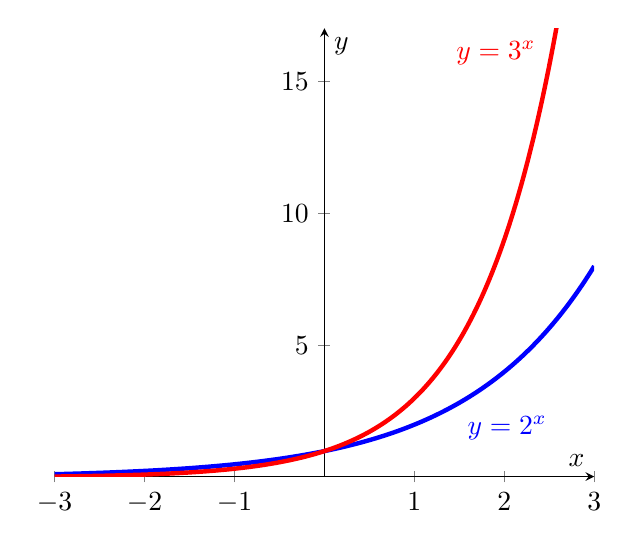
\begin{tikzpicture}
    \begin{axis}[
        axis lines=center,
        xmax = 3,
        ymax = 17,
        ylabel=$y$,
        xlabel=$x$,
        ]
        \addplot [domain=-3:3,samples=250, ultra thick, blue] {2^x}
            node [pos=0.5, below right] {$y=2^x$};
        \addplot [domain=-3:3,samples=250, ultra thick, red ] {3^x}
            node [pos=0.6, above left] {$y=3^x$};
    \end{axis}
    \end{tikzpicture}
    \end{center}

The graphs of $2^t$ and $\left(\frac{1}{3}\right)^t$ do not have as similar a shape. In particular, $\left(\frac{1}{3}\right)^t$ models exponential decay rather than exponential growth:

  %%graph of (2)^t and (1/3)^t

 \begin{center}
    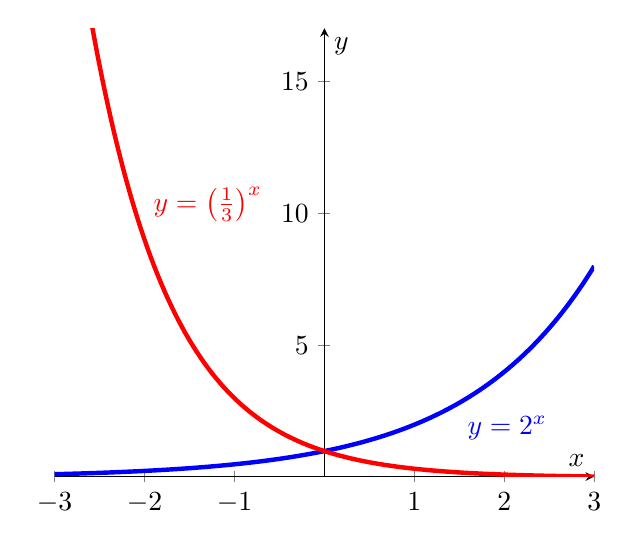
\begin{tikzpicture}
    \begin{axis}[
        axis lines=center,
        xmax = 3,
        ymax = 17,
        ylabel=$y$,
        xlabel=$x$,
        ]
        \addplot [domain=-3:3,samples=250, ultra thick, blue] {2^x}
            node [pos=0.5, below right] {$y=2^x$};
        \addplot [domain=-3:3,samples=250, ultra thick, red ] {0.3333333^x}
            node [pos=0.6, above right] {$y=\left(\frac{1}{3}\right)^x$};
    \end{axis}
    \end{tikzpicture}
    \end{center}

As a result, the coefficient $k = \log_2 (1/3)\approx -1.585$ is negative, which flips the graph of $2^{kt}$ across the vertical axis as needed. 
\end{example}

\begin{exercise}
Global human population growth amounts to around 83 million annually, or 1.1\% per year. In how many years will the population be double what it is now?
\end{exercise}


For an exponential function that models decay, it does not make sense to talk about doubling time since the values of the function are decreasing; we would have to move "backward" in time for the values of the function to double. Instead, exponential decay uses the idea of \textit{half-life}, meaning the amount of time for the values of the function to decrease by 50\%. 

\begin{example}\label{ex:introhalflife}
%\todo{intro example for half-life, so a population is decaying. start at 100 and halve, then halve again. do for arbitrary initial value.}
Radiocarbon dating (also referred to as carbon dating or carbon-14 dating) is a method for determining the age of an object containing organic material by using the properties of radiocarbon, a radioactive isotope of carbon. The method was developed in the late 1940s at the University of Chicago by Willard Libby.\footnote{Source: \href{https://en.wikipedia.org/wiki/Radiocarbon\_dating}{https://en.wikipedia.org/wiki/Radiocarbon\_dating}.}

Carbon-14 decays very slowly: about 0.0121\% per year. What is the half-life of carbon-14, meaning: how long will it take for an amount of carbon-14 to decay to half of its current mass?

Suppose that $C_0$ is the initial amount of carbon-14. The amount of carbon-14 after $t$ years is then
$$C(t) = C_0(1-0.000121)^t = C_0(0.9999879)^t.$$
We wish to find the amount of time it takes for the carbon-14 to reach a mass of $\frac{C_0}{2}$, and so we set $C(t) = \frac{C_0}{2}$ and solve for $t$:
$$\begin{aligned}
C_0(0.9999879)^t &= \frac{C_0}{2}\\
(0.9999879)^t &= \frac{C_0}{2C_0} = \frac{1}{2}\\
\log_{10}(0.9999879)^t &= \log_{10}\left( \frac{1}{2}\right)\\
t\log_{10}(0.9999879) &= \log_{10}\left( \frac{1}{2}\right)\\
t &=\frac{ \log_{10}\left( 1/2\right)}{\log_{10}(0.9999879)}\approx 57284.5
\end{aligned}$$
Thus it takes about 57284.5 years for the amount of carbon-14 to reduce by half, meaning that it has a half-life of 57284.5. 
\end{example}

\begin{exercise}
What is the quarter-life of carbon-14, meaning how long will it take for an amount of carbon-14 to become $1/4$ of its original amount?
\end{exercise}

What we saw in Example \ref{ex:introhalflife} is that it takes a fixed length of time for an exponential function to halve, meaning decrease by 50\%. This length of time is what is called the \textbf{half-life} of the function. 

%For exponential functions of the form $f(t) = A2^{kt}$, every time the exponent $kt$ increases by 1, the values of the function will be multiplied again by the base of 2. Thus when $kt$ increases by 1, the values of the function will double. When $k$ is positive, $kt$ will increase by $1$ when $t$ increases by $\frac{1}{k}$, thus the function doubles as $t$ increases. On the other hand, when $k$ is negative, $\frac{1}{k}$ is also negative so that $kt$ will increase by 1 as $t$ decreases, meaning the function will double as $t$ \textit{decreases}. Viewed another way: the function will \textit{halve} as $t$ increases by $|\frac{1}{k}|$. 
%
%\begin{example}
%Recall from the previous example that we can write
%$$g(t) = \left(\frac{1}{3}\right)^t= 2^{(\log_2 (1/3)) t}\approx 2^{-1.585 t}.$$
%Using logarithm properties to simplify $\log_2 (1/3)$, 
%$$\log_2 (1/3) = \log_2(3^{-1}) = -\log_2 3$$
%and so we see that we can write
%$$\left(\frac{1}{3}\right)^t= 2^{(-\log_2 3) t} = (2^{-1})^{(\log_2 3)t} = \left(\frac{1}{2}\right)^{(\log_2 3)t}\approx\left(\frac{1}{2}\right)^{1.585 t}$$
%Written in this form, every time the exponent $(\log_2 3) t$ increases by $1$, the function is multiplied by another $\frac{1}{2}$, and its values are halved. 
%\end{example}
%
%The length of time that it takes a function to double or halve is $|\frac{1}{k}|$. Using logarithm rules to simplify, 
%$$\begin{aligned}
%\frac{1}{k} &= \frac{1}{\log_2 b}\\
%&= \frac{\log_2 2}{\log_2 b}\\
%&= \log_b 2.
%\end{aligned}$$

%
%We summarize all of these observations in the following theorem:
%
%\begin{theorem}
%Every exponential function $f(t) = Ab^t$ can be written in the form $f(t) = A2^{kt}$, where $k = \log_2 b$. 
%\begin{itemize}
%\item When $b>1$, $k>0$ and the function $f(t)$ has a constant \textbf{doubling time}. 
%\item When $0<b<1$, $k<0$ and the function $f(t)$ has a constant \textbf{half-life}. 
%\end{itemize}
%In both cases, the time it takes for the function to double or halve is $|\log_b 2|$, meaning that the values of the function will double or halve on an interval of length $|\log_b 2|$. 
%\end{theorem}
%
%\begin{example}
%Below is a table of values for $2^x$. We can see that on every interval of length $\log_2 2 = 1$, the values of $2^x$ double (from 1 to 2, from 2 to 4, from 4 to 8, etc.):
%
%\begin{center}
%\begin{tabular}{c||ccccccc}
%$x$ & 0 & 1 & 2 & 3 & 4 & 5 & 6\\
%\hline
%$2^x$ & 1 & 2 & 4 & 8 & 16 & 32 & 64
%\end{tabular}
%\end{center}
%
%On the other hand, the values of the function $3^x$ more than double\footnote{In fact, they triple.} on an interval of length 1:
%
%\begin{center}
%\begin{tabular}{c||ccccccc}
%$x$ & 0 & 1 & 2 & 3 & 4 & 5 & 6\\
%\hline
%$3^x$ & 1 & 3 & 9 & 27 & 81 & 243 &729
%\end{tabular}
%\end{center}
%
%They will double on an interval of length $\log_3 2 = \frac{\log_{10}2}{\log_{10} 3}\approx 0.631$:
%
%\begin{center}
%\begin{tabular}{c||ccccccc}
%$x$ & 0 & $0.631$ & $1.262$ & $1.893$ & $2.524$ & $3.155$ & $3.786$\\
%\hline
%$3^x$ & 1 & $2.000$ & $4.000$ & $8.001$ & $16.005$ & $32.012$ & $64.030$
%\end{tabular}
%\end{center}
%
%\end{example}
%
%\begin{remark}
%Note that the rounding error in approximating $\log_3 2\approx 0.631$ in the above table has significant consequences for the values of the function. In general, values of exponential functions increase so rapidly that small errors in $x$-values result in large errors in values of the function. Therefore, we will always try to be as exact as possible when working with exponential functions. 
%\end{remark}
%
%\begin{example}
%The values of $\left(\frac{1}{3}\right)^x$ will not double, since the base $b=\frac{1}{3}$ is less than 1. Instead, they will halve on intervals of length $|\log_{1/3} 2| = \left|\frac{\log_{10}2}{\log_{10}(1/3)}\right|\approx|-0.631| = 0.631$:
%
%\begin{center}
%\begin{tabular}{c||ccccccc}
%$x$ & 0 & $0.631$ & $1.262$ & $1.893$ & $2.524$ & $3.155$ & $3.786$\\
%\hline
%$\left(\frac{1}{3}\right)^x$ & 1 & $0.500$ & $0.250$ & $0.125$ & $0.0625$ & $0.0312$ & $0.0156$
%\end{tabular}
%\end{center}
%
%\end{example}

We can use measures of doubling time and half-life to determine models for processes modeled by exponential functions, and use those models to predict the behavior of those processes. 

\begin{example}
Suppose a population of bacteria is growing in a petri dish in such a way that the number of bacteria doubles every 3 hours. If there are initially 1000 bacteria in the petri dish, how long will it take for there to be 1 million bacteria?

Let $B(t)$ be the number of bacteria in the dish after $t$ hours. Since $B(t)$ has a constant doubling time, we will model it with an exponential function of the form $B(t) = B_02^{kt}$ for some values $B_0$ and $k$. Moreover, we know that $B(0) = 1000$, therefore $B(t) = 1000(2)^{kt}$. Since the bacteria population doubles every three hours, $B(3) = 2B(0) = 2(1000) = 2000$. We can use this fact to solve for $k$:
$$\begin{aligned}
B(3) &= 2000\\
1000(2)^{3k} &= 2000\\
2^{3k} &= 2\\
3k &= 1\\
k &= \frac{1}{3}
\end{aligned}$$
This fits the information we are given: if $t$ is measured in hours, it takes 3 hours for the exponent $\frac{1}{3}t$ to increase one hour. 

Now we know the number of bacteria in the petri dish after $t$ hours is given by
$$B(t) = 1000(2)^{t/3}$$
and we can find out when there will be 1 million bacteria by solving the equation $B(t)= 1,000,000$ for $t$:
$$\begin{aligned}
B(t) &= 1,000,000\\
1000(2)^{t/3} &= 1,000,000\\
2^{t/3} &= 1000\\
\frac{t}{3} &= \log_2(1000)\\
t &= 3\log_2(1000)\approx 29.9
\end{aligned}$$
Therefore it will be approximately 29.9 hours before there are 1 million bacteria in the petri dish. 
\end{example}

\begin{remark}
This kind of calculation is extremely useful if you are working with cells trying to plan how long you need to wait for your sample to reach a particular size before running an assay that requires a certain number of cells, or if you want to split your sample for use in multiple experiments. In fact, the author has helped her biologist husband with such calculations in the past. His coworkers were impressed. 
\end{remark}

%\subsection{Converting between growth rate and doubling time/half-life}

It is possible to determine the doubling time/half-life of a quantity if given the percent growth rate, and vice versa. 

%\begin{example}
%Recall the population of termites from Exercise \ref{ex:Taalman5-4-1}.  We were give that the population decreased by half in the first three weeks, from 2500 at time $t=0$  to 1250 at time $t=3$.  It decreased by half again in the three weeks from $t=3$ to $t=6$, from 1250 to 625.  Then, the next three weeks from $t=6$ to $t=9$, it  decreased again by half, from 625 to 312.5. 
%
%We modeled the population by
%$$P(t)=2500(0.794)^t$$
%and we can see that our model has a half-life of $|\log_{0.794} 2| = \left|\frac{\log_{10} 2}{\log_{10}(0.794)}\right|\approx |-3.005| = 3.005$. Recall that $0.794\approx (\frac{1}{2})^{1/3}$ is an approximation, hence the small error in the half-life of our model. If we simplify the exact expression: 
%$$\log_{\sqrt[3]{1/2}} 2 = -3$$
%(we must raise $(\frac{1}{2})^{1/3} = \sqrt[3]{1/2}$ to the power of $-3$ in order to get $2$), we get a half-life of exactly $|-3| = 3$ weeks. 
%
%\end{example}





\begin{example}
%EXAMPLE 4 FROM TAALMAN SECTION 5.4 PAGES 383-384 BUT USE AN EXPONENTIAL FUNCTION WITH BASE 2, NOT E (I WILL HAVE EXPLAINED BEFORE THIS THAT FUNCTIONS WITH A BASE OF 2 HAVE CONSTANT DOUBLING TIME, AND IF YOU MAKE THE EXPONENT NEGATIVE THAT MAKES THEM DECAY SO THEY HAVE A CONSTANT HALF LIFE INSTEAD) AND BASE-2 LOGARITHMS INSTEAD OF LN. INCLUDE THE CHECKING THE ANSWER CONVERSATION. 

Radioactive substances have constant half-lives.  This means that the quantity of a radioactive substance always takes the same amount of time to decrease by half, no matter how much or how little of the substance that you start with.  For example - suppose that the half-life of the fictional substance unobtainium is 29 years.  A sample of rock is found with 80 grams of unobtainium.  Let's compute the percentage by which the amount of unobtainium in the rock decreases each year.

Let $S(t)$ represent the number of grams of unobtainium that are left after $t$ years.  Since $S(t)$ has a constant half-life, we will model $S(t)$ with an exponential function.  We also know that the initial value is $S_0=S(0)=80$ grams.  Therefore, $S(t)=80(b^{t})$ for some $b$.

We start by using the given half-life to solve for the value of the growth factor $b$.  Since unobtainium has a half-life, and we start with 80 grams of it, we know that $S(29)=\frac{S_0}{2}=40$ grams.  We use this fact to solve for $b$:

$$\begin{aligned}
S(29)=&40 \\
80(b^{29})=&40\\
b^{29}=&\frac{1}{2}\\
b &= \left(\frac{1}{2}\right)^{1/29}\\
b &= 2^{-1/29}
\end{aligned}$$

This means that the number of grams of unobtainium in the rock after $t$ years is given by the exponential function $S(t)=80(2^{-1/29})^t) = 80(2^{-t/29})$.

To find the percent decrease, we find the growth rate 
$$r = b-1 = 2^{-1/29}-1\approx -0.02362.$$ 
Therefore, the amount of unobtainium in the rock decreases by approximately 2.362\% each year.

To double check the answer we just found, we can verify that decreasing the original amount of 80 grams by 2.362\% per year for 29 years will bring us down to half the initial amount, 40 grams.  Indeed, we have 

$$S(29)=80(1-0.02362)^{29}\approx 39.9979.$$

The only reason we don't get exactly 40 grams is because we did some rounding when computing the decimal value of $r=2^{-1/29}-1$.

\end{example}



\begin{exercise}
The number of worms in a backyard garden increases every year by a percentage growth rate of 7\%. Follow the steps below to find the doubling time of the worm population. 
\begin{enumerate}[label=\alph*),itemsep=5pt]
\item Find a formula $W(t)$ for the worm population using the percent growth formula: $W(t) = W_0(1+r)^t$. \textit{You do not know the value of $W_0$, the initial quantity of worms. Leave it as an unknown constant in your formula.}
\item Solve the equation
$$  W(t) = 2W_0$$
for $t$, using the formula for $W(t) = W_0(1+r)^t$ that you found in part (a). This is the doubling time since we are finding how long it take for the worm population to double from the initial quantity $W_0$ to $2W_0$. 
\item \textbf{Check your answer:} Suppose you start with $W_0 = 100$ worms at time $t=0$. You should have approximately 200 worms after the amount of time you found in part (b), using your model from part (a). 
\end{enumerate}
\end{exercise} 


\subsection{Modeling Temperature Data}

If a quantity changes so that its growth or decay occurs at a constant percentage rate with respect to time, the function is exponential. Likewise, if a quantity doubles or halves over a constant time period, the function is exponential. 


A related situation arises when an object's temperature changes in response to its surroundings. For instance, if we have a cup of coffee at an initial temperature of 186 degrees Fahrenheit and the cup is placed in a room where the surrounding temperature is 71 degrees Fahrenheit, our intuition and experience tell us that over time the coffee will cool and eventually tend to the 71 degree Fahrenheit temperature of the surroundings. From an experiment with an actual temperature probe, we have the data in in the following table, that is plotted in the adjacent figure.
 

  \begin{table}[!htb]
  \centering
    \caption{Data for cooling coffee, measured in degrees Fahrenheit at time $t$ mintues}
         \begin{tabular}{c c c c c c c c c c c c c c}
\toprule
$t$ & 0 & 1 & 2 & 3 & 8 & 13 &18&23&28&33&38&43&48\\
\midrule
$F(t)$&186 & 179 & 175 & 171 & 156&144&135&127&120&116&111&107&104 \\
\bottomrule
\end{tabular}
      \label{tab:temp}
\end{table}

\begin{figure}[H]
\centering
         \includegraphics[width=0.5\textwidth]{ACFigure3-2-2.png}
         \caption{A plot of the data from Table \ref{tab:temp}}
         \label{}
\end{figure}

In one sense, the data looks exponential: the points appear to lie on a curve that is always decreasing and decreasing at an increasing rate. However, we know that the function can't have the form $f(t)=ab^t$,because such a function's range is the set of all positive real numbers, and it's impossible for the coffee's temperature to fall below room temperature (71 degrees).  It is natural to wonder if a function of the form $g(t)=ab^t+c$ will work. 

%SKIP TO SECTION 3.2.2: INCLUDE THE FIRST PARAGRAPH EXCEPT FOR "and then make the following general observations." AND THE TWO PICTURES BELOW IT. DO NOT INCLUDE BOX OF OBSERVATIONS. 

The function $g(t)=ab^t+c$ is a vertical translation of the function $f(t)=ab^t$. We now have extensive understanding of the behavior of $f(t)$, and how that behavior depends on $a$ and $b$. Since a vertical translation by $c$ does not change the shape of any graph, we expect that $g$ will exhibit very similar behavior to $f$,  Indeed, we can compare the two functions' graphs, as shown in the following figures.

\begin{figure}[H]
     \centering
     \begin{subfigure}[b]{0.4\textwidth}
         \centering
         \includegraphics[width=\textwidth]{ACFigure3-2-6.png}
         \caption{Plot of $f(t)=ab^t$}
         \label{}
     \end{subfigure}
     \hfill
     \begin{subfigure}[b]{0.4\textwidth}
         \centering
         \includegraphics[width=\textwidth]{ACFigure3-2-7.png}
         \caption{Plot of $g(t)=ab^t+c$}
         \label{}
     \end{subfigure}

\end{figure} 
 
%SKIP TO SECTION 3.2.3. THIS UP THROUGH ACTIVITY 3.2.3. NOT SURE IF THIS WILL BE AN EXAMPLE OR EXERCISE YET. IF YOU HAVE TIME, TYPE IN SOLUTIONS, IF NOT, DON'T. (Activity 3.2.4 will go on the worksheet, I think)

Newton's Law of Cooling states that the rate that an object warms or cools occurs in direct proportion to the difference between its own temperature and the temperature of its surroundings. If we return to the coffee temperature data in Table \ref{tab:temp} and recall that the room temperature in that experiment was $71$ degrees Fahrenheit, we can see how to use a transformed exponential function to model the data. In Table \ref{tab:tempshifted}, we add a row of information to the table where we compute $F(t)-71$ to subtract the room temperature from each reading.
 
   \begin{table}[!htb]
  \centering
    \caption{Data for cooling coffee, measured in degrees Fahrenheit at time $t$ mintues}
         \begin{tabular}{c c c c c c c c c c c c c c}
\toprule
$t$ & 0 & 1 & 2 & 3 & 8 & 13 &18&23&28&33&38&43&48\\
\midrule
$F(t)$&186 & 179 & 175 & 171 & 156&144&135&127&120&116&111&107&104 \\
\midrule
$f(t)=F(t)-71$&115 & 108 & 104 & 100 & 85&73&64&56&49&45&40&36&33 \\
\bottomrule
\end{tabular}
      \label{tab:tempshifted}
\end{table}

The data in the bottom row of Table \ref{tab:tempshifted} appears exponential, and if we test the data by computing the quotients of output values that correspond to equally-spaced input, we see a nearly constant ratio. In particular,

$$\frac{73}{85}\approx0.86, \ \ \frac{64}{73}\approx0.88, \ \ \frac{56}{64}\approx0.88, \ \ \frac{49}{56}\approx0.88, \ \ \frac{45}{49}\approx0.92,  \textrm{ and }\frac{40}{55}\approx0.89.$$

Of course, there is some measurement error in the data (plus it is only recorded to accuracy of whole degrees), so these computations provide convincing evidence that the underlying function is exponential. In addition, we expect that if the data continued in the bottom row of Table \ref{tab:tempshifted}, the values would approach $0$ because $F(t)$ will approach 71.

\begin{figure}[H]
     \centering
     \begin{subfigure}[b]{0.4\textwidth}
         \centering
         \includegraphics[width=\textwidth]{ACFigure3-2-9.png}
         \caption{Plot of $f(t)=103.503(0.974)^t$}
         \label{fig:temp}
     \end{subfigure}
     \hfill
     \begin{subfigure}[b]{0.4\textwidth}
         \centering
         \includegraphics[width=\textwidth]{ACFigure3-2-10.png}
         \caption{Plot of $F(t)=103.503(0.974)^t+71$}
         \label{fig:tempshifted}
     \end{subfigure}

\end{figure} 

If we choose two of the data points, say $(18,64)$ and $(23, 56)$, and assume that $f(t)=ab^t$, we can determine the values of $a$ and $b$. Doing so, it turns out that $a\approx103,503$ and $b\approx0.974$, so that $f(t)=103.503(0.974)^t$.  Since $f(t)=F(t)-71$, we can see that $F(t)=f(t)+71=103.503(0.974)^t+71$. Plotting $f$ against the shifted data and $F$ along with the original data in Figure \ref{fig:temp} and Figure \ref{fig:tempshifted}, we see that the curves go exactly through the points where $t=18$ and $t=23$ as expected, but also that the function provides a reasonable model for the observed behavior at any time $t$. If our data was even more accurate, we would expect that the curve's fit would be even better.

Our preceding work with the coffee data can be done similarly with data for any cooling or warming object whose temperature initially differs from its surroundings. Indeed, it is possible to show that Newton's Law of Cooling implies that the object's temperature is given by a function of the form $F(t)=ab^t+c$.

\begin{exercise}\label{ex:tempmodeling}
A can of soda (at room temperature) is placed in a refrigerator at time $t=0$ (in minutes) and its temperature, $F(t)$, in degrees Fahrenheit, is computed at regular intervals. Based on the data, a model is formulated for the object's temperature, given by

$$F(t)=42+30(0.95)^t.$$

\begin{enumerate}[label=\alph*),itemsep=5pt]
\item Consider the simpler (parent) function $p(t)=(0.95)^t$.  How do you expect the graph of this function to appear? How will it behave as time increases? Without using graphing technology, sketch a rough graph of $p$, and write a sentence of explanation.
\item For the slightly more complicated function $r(t)=30(0.95)^t$, how do you expect this function to look in comparison to $p$?What is the long-range behavior of this function as $t$ increases? Without using graphing technology, sketch a rough graph of $r$ and write a sentence of explanation.
\item Finally, how do you expect the graph of $F(t)=42+30(0.95)^t$ to appear? Why? First sketch a rough graph without graphing technology, and then use technology to check your thinking.
\item What is the temperature of the refrigerator? What is the room temperature of the surroundings outside the refrigerator? Why?
%\item Determine the average rate of change of $F$ on the intervals $[10,20]$, $[20,30]$, and $[30,40]$. Write at least two careful sentences that explain the meaning of the values you found, including units, and discuss any overall trend in how the average rate of change is changing.
 \end{enumerate}
 
\end{exercise}



\subsection{Measuring Earthquakes and Sound}

%Sources:
%http://content.nroc.org/DevelopmentalMath/COURSE_TEXT2_RESOURCE/U18_L4_T2_text_container.html
%https://www.sms-tsunami-warning.com/pages/richter-scale
%https://www.youtube.com/watch?v=l9J4YG5WsIU

Logarithmic functions are also used to model real-world phenomena. One of the most commonly used such models is the Richter magnitude scale (often shortened to Richter scale), used to rate the magnitude of an earthquake, that is the amount of energy released during an earthquake.Another model is the unit of measurement called a decibel, which is used to measure sound.\footnote{Sources: \href{https://www.sms-tsunami-warning.com/pages/richter-scale}{https://www.sms-tsunami-warning.com/pages/richter-scale} and \\
\href{http://content.nroc.org/DevelopmentalMath/COURSE\_TEXT2\_RESOURCE/U18\_L4\_T2\_text\_container.html}{http://content.nroc.org/DevelopmentalMath/COURSE\_TEXT2\_RESOURCE/U18\_L4\_T2\_text\_container.html}. Additional examples from \href{https://www.youtube.com/watch?v=l9J4YG5WsIU}{https://www.youtube.com/watch?v=l9J4YG5WsIU}.}



Let’s look at the \textbf{Richter scale}, a logarithmic function that is used to measure the magnitude of earthquakes. The magnitude of an earthquake is related to how much energy is released by the quake. Instruments called seismographs detect movement in the earth. If the smallest movement that can be detected shows on a seismograph as a wave with amplitude $A_0$, and we let $A$ be the measure of the amplitude of an earthquake wave, then
$$R=\log_{10}\left(\frac{A}{A_0}\right)$$
is the Richter scale measure of the magnitude of the earthquake. Note that this formula makes use of the relative size of the amplitude $A$ of the earthquake being measured to the amplitude of the smallest detectable wave, called a \textit{standard wave}. 

Using the logarithm rules, we can rewrite the formula for the Richter scale as
$$R = \log_{10}A-\log_{10}A_0.$$
Since $A_0$ is some fixed number (depending on the seismograph being used), $\log_{10}A_0$ is also a fixed number. Thus the increase in the Richter scale depends only on the term $\log_{10}A$ and we see that the Richter scale is a base-10 logarithmic scale, meaning that each order of magnitude is 10 times more intensive than the last one. In other words, a two is 10 times more intense than a one and a three is 100 times greater. In the case of the Richter scale, the increase is in wave amplitude. That is, the wave amplitude in a level 6 earthquake is 10 times greater than in a level 5 earthquake, and the amplitude increases 100 times between a level 7 earthquake and a level 9 earthquake. 

\begin{example}
An earthquake is measured with a wave amplitude 392 times as great as $A_0$. What is the magnitude of this earthquake using the Richter scale, to the nearest tenth?

\begin{solution}
Since $A$ is 392 times as large as $A_0$, $A = 392A_0$. Substituting this expression in for $A$:
$$R=\log_{10}\left(\frac{392A_0}{A_0}\right) = \log_{10}(392)\approx 2.6.$$
\end{solution}
\end{example}

A difference of 1 point on the Richter scale equates to a 10-fold difference in the amplitude of the earthquake (which is related to the wave strength). This means that an earthquake that measures 3.6 on the Richter scale has 10 times the amplitude of one that measures 2.6.

 \begin{example}
 Let’s look back at the previous example. In that example, the wave amplitude of the earthquake was 392 times normal. What if it were 10 times that, or 3,920 times normal? To find the measurement of that size earthquake on the Richter scale, you find 
 $$R = \log_{10}\left(\frac{ 3920A_0}{A_0}\right) = \log_{10}(3920)\approx 3.6.$$
 
 Thus one point on the Richter scale corresponds to a much, much more intense earthquake!
 \end{example}


The Richter scale is particularly useful in allowing us to measure the magnitude of earthquakes relative to each other. 

\begin{example}
An earthquake on July 30, 2018 in California measured 3.7 on the Richter scale. If an earthquake is 16,550 times more powerful than the California earthquake, what would be its magnitude on the Richter scale?

\begin{solution}
Suppose that the California earthquake had maximum wave amplitude of $C$. Then the Richter scale magnitude of the California earthquake tells us that 
$$\begin{aligned}
3.7 &= \log_{10}\left(\frac{C}{A_0}\right)\\
&= \log_{10}C - \log_{10}A_0
\end{aligned}$$
The magnitude $A$ of the earthquake we wish to measure is 16,550 times more powerful, meaning that
$$A = 16550C.$$
Substituting this into the Richter scale measurement for $A$, we are able to expand via the logarithm rules:
$$\begin{aligned}
R &= \log_{10}\left(\frac{A}{A_0}\right) \\
&=\log_{10}\left(\frac{16550C}{A_0}\right)\\
&= \log_{10}(16550)+\log_{10}C-\log_{10}A_0
\end{aligned}$$
However we already know that $\log_{10}C-\log_{10}A_0=3.7$, so in measuring $R$, we need only add $\log_{10}(16550)$ to the previous measurement of 3.7:
$$R = \log_{10}(16550)+3.7\approx 4.2+3.7 = 7.9.$$
\end{solution}
\end{example}

In general, in order to determine the Richter scale magnitude of an earthquake that is $m$ times more powerful than an earthquake with Richter scale measurement $R_0$, we must simply add $\log_{10}m$:
$$R = \log_{10}m+R_0.$$

\begin{exercise}
On March 22, 2011, an earthquake in Japan measured a 9.1 on the Richter scale. What is the Richter scale magnitude of an earthquake that is 100,000 times \textit{weaker} than the Japan earthquake? \textit{This means that $A=J/100000$, where $A$ is the maximum wave amplitude of the earthquake we wish to measure and $J$ is the maximum wave amplitude of the earthquake in Japan.}
\end{exercise}



The formula for \textbf{decibels} looks very similar to the Richter scale:
$$d=10\log_{10}\left(\frac{P}{P_0}\right)$$
where $P$ is the power or intensity of the sound and $P_0$ is the weakest sound that the human ear can hear.

\begin{example}
One hot water pump has a noise rating of 50 decibels. One dishwasher, however, has a noise rating of 62 decibels. The dishwasher noise is how many times more intense than the hot water pump noise?

\begin{solution}
You can’t easily compare the two noises using the formula, but you can compare them to $P_0$. Start by finding the intensity of noise for the hot water pump. Use $H$ for the intensity of the hot water pump’s noise. Then
$$\begin{aligned}
50 &=10\log_{10}\left(\frac{H}{P_0}\right)\\
5 &= \log_{10}\left(\frac{H}{P_0}\right)
\end{aligned}
$$
And rewriting in terms of exponents:
$$\begin{aligned}
10^5 &= \frac{H}{P_0}\\
10^5P_0 &= H
\end{aligned}$$
We repeat the same process to find the intensity $D$ of the noise for the dishwasher:
$$\begin{aligned}
62 &= 10\log_{10}\left(\frac{D}{P_0}\right)\\
6.2 &= \log_{10}\left(\frac{D}{P_0}\right)\\
10^{6.2} &= \frac{D}{P_0}\\
10^{6.2}P_0 &= D
\end{aligned}$$
Now to compare $D$ to $H$, we can divide:
$$\begin{aligned}
\frac{D}{H} &= \frac{10^{6.2}P_0}{10^5P_0}\\
&= 10^{1.2}
\end{aligned}$$

Thus we see that the dishwasher's noise is $10^{1.2}\approx 15.85$ times as intense as the hot water pump.
\end{solution}
\end{example}

With decibels, every increase of 10 means the sound is 10 times more intense. An increase of 20 would be 10 times more intense for the first 10, and another 10 times more intense for the second 1 --so a sound that is 75 decibels is 100 times more intense than a sound that is 55 decibels!

\begin{example}
%Library/LoyolaChicago/Precalc/Chap4Sec3/Q36.pg.
Let $D_1$ and $D_2$ represent the decibel ratings of sound intensity $P_1$ and $P_2$, respectively. Using logarithm rules, we can find a simplified formula for the difference between the two ratings $D_1$ and $D_2$ as follows:
$$\begin{aligned}
D_1-D_2 &= 10\log_{10}\left(\frac{P_1}{P_0}\right)-10\log_{10}\left(\frac{P_2}{P_0}\right)\\
&= 10(\log_{10}P_1 - \log_{10}P_0) - 10(\log_{10}P_2-\log_{10}P_0)\\
&= 10(\log_{10}P_1 - \log_{10}P_2)\\
&= 10\log_{10}\left(\frac{P_1}{P_2}\right)
\end{aligned}$$

If a sound's intensity triples, how many decibels louder does the sound become? In other words, what is $D_1-D_2$ if $P_1=3P_2$? Using the above formula, 
$$\begin{aligned}
D_1-D_2  &= 10\log_{10}\left(\frac{P_1}{P_2}\right)\\
&= 10\log_{10}\left(\frac{3P_2}{P_2}\right)\\
&= 10\log_{10}(3)\\
&\approx 4.77
\end{aligned}$$

Thus the sound becomes about 4.77 decibels louder. 
\end{example}


\subsection*{Summary}
The following terms were introduced in this section: 
\begin{quotation}
doubling time, half-life; Richter scale, decibel. 
\end{quotation}

\textbf{Key ideas:} Exponential functions model percent growth, and thus have constant doubling time (in the case of exponential growth) or half-life (in the case of exponential decay). Transformations of exponential functions can be used to model the temperature of an object being heated or cooled. Logarithms are used to measure magnitudes of earthquakes and intensities of sound.  

\textbf{Other ideas reinforced:} Logarithm rules, and the relationship between exponential and logarithmic functions. 




\begin{center}
\textcolor{ocre}{\fbox{\fbox{\Large \bf \sc End of Section 5.4}}}
\end{center}

\hspace{-.5in}\rule{1.1\textwidth}{2pt}













%----------------------------------------------------------------------------------------
%	Section 5
%----------------------------------------------------------------------------------------


\section{Limits of exponential and logarithmic functions}


\subsection*{Learning Goals}

\begin{itemize}
	\item Understand limits of exponential growth vs. decay functions via reflections, and limits of logarithmic functions via properties of inverse functions. 
	\item Calculate limits of exponential and logarithmic functions at the edges of their domains, and visualize these limits as vertical and/or horizontal asymptotes on graphs. 
	\item Apply these new limits to old techniques for evaluating indeterminate limits forms. 
\end{itemize}


\subsection{Exponential and Logarithmic Functions are Continuous on their Domains}




Similar to the algebraic functions we worked with in the fall, exponential and logarithmic functions are continuous on their domains. Note in particular that their graphs do not have any jumps or holes on their domains. 

\begin{theorem}[Continuity of Exponential and Logarithmic Functions]
All exponential and logarithmic functions are continuous on their domains.
\end{theorem}

%EXERCISE: CALCULATE EACH OF THE FOLLOWING LIMITS, OR EXPLAIN WHY THE LIMIT DOES NOT EXIST (TWO LIMITS OF EXPONENTIAL FUNCTIONS WHERE THEY ARE DEFINED, ONE BASE GREATER THAN 1, ONE BASE LESS THAN 1, ONE LIMIT OF A LOGARITHM WHERE IT'S DEFINED, ONE LIMIT OF A LOGARITHM WHERE IT'S NOT DEFINED - OUTSIDE OF ITS DOMAIN, NOT THE ASYMPTOTE)

Remember that, practically speaking, if a function $f(x)$ is continuous at $x=a$ it means that we can evaluate the limit by evaluation $\ds\lim_{x\to a}f(x) = f(a)$, provided that $f(a)$ is defined. 

\begin{exercise}
Calculate each of the limits below by evaluation and simplifying, or explain why the expression is undefined. 

\begin{multicols}{2}
\begin{enumerate}[label=\alph*.,itemsep=10pt,topsep=5pt]
\item $\ds\lim_{x\to 3} (3(25)^{-x/2}+1)$
\item $\ds\lim_{x\to -4} \left(\frac{2}{3}\right)^x$
\item $\ds\lim_{x\to 2}\ \log_2(x^2-1)$
\item $\ds\lim_{x\to 0}\ \log_2(x^2-1)$
\end{enumerate}
\end{multicols}
\end{exercise}

\subsection{Limits at Infinity of Exponential Functions}

%APC 3.2.1 \url{https://activecalculus.org/prelude/sec-exp-modeling.html}: DISCUSSES LIMITS AT INFINITY OF EXPONENTIAL FUNCTIONS WITH DIFFERENT BASES

We have already established that any exponential function of the form $f(t) = ab^t$ where $a$ and $b$ are positive real numbers with $b\neq 1$ is always concave up and is either always increasing or always decreasing. We next introduce precise language to describe the behavior of an exponential function's value as $t$ gets bigger and bigger. To start, let's consider the two basic exponential functions $p(t) = 2^t$ and $q(t) = \left(\frac{1}{2}\right)^t$ and their respective values at $t=10, t=20$, and $t=30$, as displayed below:


\begin{center}
\includegraphics[width=5in]{APC3-2-1Tables.png}
\end{center}

For the increasing function $p(t) = 2^t$, we see that the output of the function gets very large very quickly. In addition, there is no upper bound to how large the function can be. Indeed, we can make the value of $p(t)$ as large as we'd like by taking $t$ sufficiently big. We thus say that as $t$ increases, $p(t)$ \textit{increases without bound} and write
$$\lim_{t\to\infty}2^t = \infty.$$

For the decreasing function $q(t) = \left(\frac{1}{2}\right)^t$, we see that the output $q(t)$ is always positive but getting closer and closer to 0. Indeed, because we can make $2^t$ as large as we like, it follows that we can make its reciprocal $\frac{1}{2^t} = \left(\frac{1}{2}\right)^t$ as small as we'd like. We thus say that as $t$ increases, $q(t)$ \textit{approaches 0}. We write
$$\lim_{t\to\infty}\left(\frac{1}{2}\right)^t = 0.$$

We've seen several times how the value of $b$ affects the steepness of the graph of $f(t) = ab^t$, as well as how all graphs with $b>1$ have the similar increasing behavior, and all graphs with $0<b<1$ have similar decreasing behavior. For instance, by taking $t$ sufficiently large, we can make $(1.01)^t$ as large as we want; it just takes much larger values of $t$ to make $(1.01)^t$ big in comparison to $2^t$. In the same way, we can make $(0.99)^t$ as close to $0$ as we wish by taking $t$ sufficiently big, even though it takes longer for $(0.99)^t$ to get close to $0$ in comparison to $\left(\frac{1}{2}\right)^t$. For an arbitrary choice of $b$, we can say the following:

\begin{theorem}[Limits at Infinity of $b^t$]\label{thm:expatinfinity}
Let $f(t) = b^t$ with $b>0$ and $b\neq 1$. 
\begin{enumerate}[label=\textbf{\alph*.},itemsep=10pt,topsep=5pt]
\item If $0<b<1$, then $\ds\lim_{t\to\infty}b^t = 0$. 
\item If $b>1$, then $\ds\lim_{t\to\infty}b^t = \infty$. 
\end{enumerate}
\end{theorem}

In addition, we make a key observation about the use of exponents. For the function $q(t) = \left(\frac{1}{2}\right)^t$, there are three equivalent ways we may write the function:
$$\left(\frac{1}{2}\right)^t = \frac{1}{2^t} = 2^{-t}.$$
Now we can see that $q(t) = 2^{-t} = q(-t)$. Recall that the graph of a function $y=h(-t)$ is the reflection of the graph of $y=h(t)$ across the $y$-axis. Therefore, we can say that the graphs of $p(t) = 2^t$ and $q(t) = \left(\frac{1}{2}\right)^t = 2^{-t}$ are reflections of one another in the $y$-axis since $p(-t) = 2^{-t} = q(t)$. We see this fact verified in the picture below:

\begin{figure}[H]
\centering
\includegraphics[width=2in]{APCFigure3-2-5.png}
\caption{The graph of $q(t) = 2^{-t}$ is the graph of $p(t) = 2^t$ reflected across the $y$-axis, and vice versa.}
\label{fig:APCFigure3-2-5}
\end{figure}

Similar observations hold for the relationship between the graphs of $b^t$ and $\frac{1}{b^t} = b^{-t}$ for any $b\neq 1$. This allows us to analyze the limits at $-\infty$ of functions $f(t) = b^t$ quickly, using what we already know. For example, if $b>1$, we know that $0<\frac{1}{b}<1$ and hence
$$\lim_{t\to\infty}\left(\frac{1}{b}\right)^t = \lim_{t\to\infty} b^{-t} = 0$$
Reflecting this across the $y$-axis, we see then that
$$\lim_{t\to-\infty} b^t = 0$$
A similar statement holds for $0<b<1$, with the infinite limit of the exponential growth at infinity reflecting over the $y$-axis to the infinite limit of exponential decay at negative infinity (see the graphs in Figure \ref{fig:APCFigure3-2-5} to visualize this). Summarizing these observations:

\begin{theorem}[Limits at Negative Infinity of $b^t$]\label{thm:expatnegativeinfinity}
Let $f(t) = b^t$ with $b>0$ and $b\neq 1$. 
\begin{enumerate}[label=\textbf{\alph*.},itemsep=10pt,topsep=5pt]
\item If $0<b<1$, then $\ds\lim_{t\to-\infty}b^t = \infty$. 
\item If $b>1$, then $\ds\lim_{t\to-\infty}b^t = 0$. 
\end{enumerate}
\end{theorem}

\begin{remark}
It is very important and so we reiterate it again: values of $b^t$ are always positive, even for negative values of the exponent $t$. 
\end{remark}

Theorems \ref{thm:expatinfinity} and \ref{thm:expatnegativeinfinity} are easier to remember in pictures than in symbols.  Pay special attention to the values of $b$ that apply to each picture.  What the above theorems say is that the "ends" of the graphs of exponential functions behave like this:




\begin{figure}[H]
	\centering
	\begin{subfigure}[H]{0.4\textwidth}
    		\centering
    		\includegraphics[width=0.7\textwidth]{TaalmanPage355a-1.png}
    		\caption{For $b>1$, $\lim_{x\to\infty}b^x=\infty$ and $\lim_{x\to-\infty}b^x=0$.}
    		\label{fig:TaalmanPage355a-1}
	\end{subfigure}
	\hspace{.5in}
	\begin{subfigure}[H]{0.4\textwidth}
    		\centering
    		\includegraphics[width=0.7\textwidth]{TaalmanPage355a-2.png}
    		\caption{For $0<b<1$, $\lim_{x\to\infty}b^x=0$ and $\lim_{x\to-\infty}b^x=\infty$.}
    		\label{fig:TaalmanPage355a-2}
	\end{subfigure}
\caption{Limits of $b^x$ at $\infty$ and $-\infty$ are best remembered visually.}
\label{fig:TaalmanPage355a}
\end{figure}


Another way to write these Theorems \ref{thm:expatinfinity} and \ref{thm:expatnegativeinfinity} is in terms of base-2 exponential functions $f(t) = 2^{kt}$. If we insist that $k>0$ is a \textit{positive} number, then we have observed that $b^t = 2^{kt}$ when $b>1$, and that $b^t = 2^{-kt}$ when $0<b<1$. Rewriting Theorems \ref{thm:expatinfinity} and \ref{thm:expatnegativeinfinity}:

\begin{theorem}[Limits of Base-2 Exponential Functions at Infinity and Negative Infinity]
If $k$ is a positive real number, then
\begin{enumerate}[label=\textbf{\alph*.},itemsep=10pt,topsep=5pt]
\item $\ds\lim_{t\to\infty}2^{kt} = \infty$ and $\ds\lim_{t\to-\infty} 2^{kt} = 0$. 
\item $\ds\lim_{t\to\infty}2^{-kt} = 0$ and $\ds\lim_{t\to-\infty} 2^{-kt} = \infty$. 
\end{enumerate}

\end{theorem}


The following example is intended to remind us how finite limits at $\infty$ and $-\infty$ can be interpreted visually as horizontal asymptotes: 


\begin{example}
Consider the function $f(x)=\frac{3}{2+2^{-4x}}$.  What are the horizontal asymptotes of $f(x)$? 

\begin{solution}
 To find horizontal asymptotes, we must compute the limit of $f(x)$ as $x\to \infty$ as well as $x\to-\infty$.  

As $x\to \infty$, note that 
$$\lim_{x\to \infty} 2^{-4x} = 0$$
so that
$$\lim_{x\to\infty}f(x)=\lim_{x\to\infty}\frac{3}{2+2^{-4x}}=\frac{3}{2+0}=\frac{3}{2}.$$

As $x\to- \infty$, note that
$$\lim_{x\to -\infty} 2^{-4x} = \infty$$
so that
$$\lim_{x\to-\infty}f(x)=\lim_{x\to-\infty}\frac{3}{2+2^{-4x}}=\frac{3}{2+\infty}=\frac{3}{\infty}=0.$$

The graph of $f(x)=\frac{3}{2+2^{-4x}}$ therefore has \textit{two different horizontal asymptotes} to the right and left.  To the right there is an asymptote at $y=\frac{3}{2}$, and to the left there is an asymptote at $y=0$.  We can check this by looking at the graph:

\begin{figure}[H]
         \centering
         \includegraphics[width=2in]{TaalmanPage359.png}
         \caption{$f(x)=\frac{3}{2+2^{-4x}}$ has two different horizontal asymptotes to the right and left.}
\end{figure}

Notice that the graph does indeed have a horizontal asymptotes to the right at $y=\frac{3}{2}$ and to the left at $y=0$.
\end{solution}

\end{example}

%EXERCISE: RECALL TEMPERATURE MODELING EXERCISE FROM SECTION 6.4. VERIFY THAT THE LIMIT AT INFINITY GOES TO THE NUMBER THAT MAKES SENSE IN CONTEXT. WHAT IS THE LIMIT AT NEGATIVE INFINITY? IS THIS REALISTIC IN THE CONTEXT OF MODELING TEMPERATURE? 



\begin{exercise}
Recall the can of soda from Exercise \ref{ex:tempmodeling}: 

A can of soda (at room temperature) is placed in a refrigerator at time $t=0$ (in minutes) and its temperature, $F(t)$, in degrees Fahrenheit, is computed at regular intervals. Based on the data, a model is formulated for the object's temperature, given by

$$F(t)=42+30(0.95)^t.$$

\begin{enumerate}[label=\alph*),itemsep=5pt]
\item Calculate $\ds\lim_{t\to\infty}F(t)$. What does this tell you in the context of the can of soda? Does this make sense? \textit{Look back at your answers for Exercise \ref{ex:tempmodeling} and find the temperature of the refrigerator.}
\item Calculate $\ds\lim_{t\to-\infty}F(t)$. Is this realistic in the context of the can of soda? Why or why not?
\end{enumerate}
\end{exercise}

\subsection{Limits of Logarithmic Functions}

We know that we can calculate limits of logarithmic functions at domain points simply by evaluation. What about non-domain points? Logarithmic functions have domain $(0,\infty)$, so we need to examine their limits as $x\to0^+$ and as $x\to\infty$. 

%DISCUSSION OF LOG BASE B WHERE B IS GREATER THAN 1:
%
%FROM 6.3.1:
Consider $b=2$. Because the graph of $f(x) = 2^x$ increases more and more rapidly as $x$ increases, the graph of $\log_2{x}$ increases more slowly as $x$ increases. Even though the logarithmic function grows very slowly, it grows without bound because we can make $\log_2 x$ as large as we want by making $x$ sufficiently large. For instance, if we want $x$ such that $\log_2(x) = 100$, we choose $x=2^{100}$, since $\log_2(2^{100}) = 100.$

\begin{center}
\begin{tabular}{c|c|c|c|c|c|c|c|c|c|c|c}
$x$ & $2^{10}$ & $2^{100}$ & $2^{1,000}$ & $2^{10,000}$ & $2^{100,000}$ & $2^{1,000,000}$ & $\to\infty$\\
\hline
$\log_2(x)$ & 10&100 &  1,000& 10,000 &100,000  & 1,000,000 &  $\to\infty$
\end{tabular}
\end{center}

Using this table, we can see that as $x\to\infty$, $\log_2(x)\to\infty.$  Using limit notation, this means that $$\displaystyle\lim_{x\to\infty}\log_2(x)=\infty.$$ 



%DISCUSSION OF WHAT HAPPENS AT 0 FROM THE RIGHT WHEN VIEWED AS INVERSE OF EXPONENTIAL FUNCTION OF BASE 2. 

On the other hand, we saw that $\ds\lim_{x\to-\infty}2^x = 0$, meaning that when the input of $f(x) = 2^x$ becomes large and negative, the output becomes closer and closer to 0. Recall that since $2^x$ is always positive, the output is approaching 0 and is positive, which we can write as $\ds\lim_{x\to\infty} 2^x = 0^+$. 

Using our understanding of inverse functions as swapping input and output, this tells us that as the inputs of $f^{-1}(x) = \log_2 x$ approach 0 and are positive, the values of the output will become large and negative. Written as a limit:
$$\lim_{x\to 0^+}\log_2 x = -\infty.$$

In words, this tells us that we can make the values of $\log_2 x$ as large and \textit{negative} as we want by making $x$ sufficiently small, meaning sufficiently close to 0. For instance, if we want $x$ such that $\log_2(x) = -100$, we choose $x = 2^{-100}$, since $\log_2(2^{-100}) = -100$. If we want $x$ such that $\log_2(x) = -1,000$, we choose $x=2^{-1000}$, since $\log_2(2^{-1000}) = -1000$. (Recall that $2^{-100} = \frac{1}{2^{100}}$ is positive and very, very close to zero. $2^{-1000}$ is even close to 0.) Thus as the inputs of $x$ approach $0$ and are positive, the values of $2^x$ become infinitely large and negative, as illustrated in Table \ref{tab:zerolimitoflog2}:

\begin{table}[H]
\centering
\begin{tabular}{c|c|c|c|c|c|c|c|c|c|c|c}
$x$ & $2^{-10}$ & $2^{-100}$ & $2^{-1,000}$ & $2^{-10,000}$ & $2^{-100,000}$ & $2^{-1,000,000}$ & $\to0^+$\\
\hline
$\log_2(x)$ & $-10$&$-100$ &  $-1,000$& $-10,000$ &$-100,000$  & $-1,000,000$ &  $\to-\infty$
\end{tabular}
\caption{$\lim_{x\to0^+}2^x = -\infty.$}
\label{tab:zerolimitoflog2}
\end{table}

There is of course nothing special about the base $2$, and the above observations apply to logarithms of any base $b$ with $b>1$. When $0<b<1$, we have a different behavior, similar to the different behavior for exponential functions of base $0<b<1$:

$$\lim_{x\to\infty} \left(\frac{1}{2}\right)^x = 0^+ \qquad\text{ and so }\qquad \lim_{x\to0^+}\log_{1/2}x = \infty$$
and
$$\lim_{x\to-\infty} \left(\frac{1}{2}\right)^x =\infty\qquad\text{ and so }\qquad \lim_{x\to\infty}\log_{1/2}x = -\infty$$


Similarly to before, these limits are best remembered via pictures:

%\begin{center}
%\includegraphics[width=2.5in]{TaalmanPage355b.png}
%\end{center}



\begin{figure}[H]
	\centering
	\begin{subfigure}[H]{0.4\textwidth}
    		\centering
    		\includegraphics[width=0.7\textwidth]{TaalmanPage355b-1.png}
    		\caption{For $b>1$, $\lim_{x\to\infty}\log_bx=\infty$ and $\lim_{x\to0^+}b^x=-\infty$.}
    		\label{fig:TaalmanPage355b-1}
	\end{subfigure}
	\hspace{.5in}
	\begin{subfigure}[H]{0.4\textwidth}
    		\centering
    		\includegraphics[width=0.7\textwidth]{TaalmanPage355b-2.png}
    		\caption{For $0<b<1$, $\lim_{x\to\infty}\log_bx=-\infty$ and $\lim_{x\to0^+}b^x=\infty$.}
    		\label{fig:TaalmanPage355b-2}
	\end{subfigure}
\caption{Limits of $\log_bx$ at $\infty$ and $0^+$ are best remembered visually.}
\label{fig:TaalmanPage355b}
\end{figure}

Finally, we summarize these observations in the following theorem:

\begin{theorem}[Limits of Logarithmic functions at Infinity and Zero]\label{thm:limlog}

Let $b>0$.
\begin{enumerate}[label=\textbf{\alph*)},itemsep=10pt,topsep=5pt]
\item If $b>1$, then $\displaystyle\lim_{x\to\infty}\log_bx=\infty$ and $\displaystyle\lim_{x\to0^+}\log_bx=-\infty$.
\item If $0<b<1$, then $\displaystyle\lim_{x\to\infty}\log_bx=-\infty$ and $\displaystyle\lim_{x\to0^+}\log_bx=\infty$.
\end{enumerate}

\end{theorem}

%REMARK: LOGARITHMIC FUNCTIONS HAVE VERTICAL ASYMPTOTES WHEN THEIR ARGUMENTS APPROACH 0 FROM THE RIGHT. 

\noindent
\fbox{\parbox{6in}{
Something rather unexpected occurs for logarithms: they have vertical asymptotes! Previously, we have only encountered vertical asymptotes arising as the result of division by a quantity approaching zero. Add this fact to your collection of knowledge relating to vertical asymptotes: logarithmic functions have vertical asymptotes when their \textbf{arguments}, meaning the value the logarithm takes as input, approach 0 from the right. 
}}


\begin{example}
Consider the function $h(x) = \log_2(x^2-1)$. This can be viewed as a composition $f\circ g$ where $f(x) = \log_2 x$ and $g(x) = x^2-1$. 

The \textbf{argument} of the logarithm in $h(x) = \log_2(x^2-1)$ is the expression $x^2-1$, and the values of this argument determine whether $h(x)$ has a vertical asymptote

We have established that $f(x) = \log_2x$ has a vertical asymptote at $x=0$ for $x>0$. 

$g(x) = x^2-1=0$ for $x=\pm 1$ and we can check via a sign chart that $x^2-1>0$ for $x<-1$ and for $x>1$. 

Thus the composite function $h(x) = f(g(x) = \log_2(x^2-1)$ will have vertical asymptotes at $x=-1$ and $x=1$, but only on the sides where $x^2-1>0$, meaning from the left of $x=-1$ and the right of $x=1$. 

We see this illustrated in the graph below:

\begin{figure}[H]
\centering
\includegraphics[width=3in]{LogVAs.png}
\caption{$h(x) = \log_2(x^2-1)$ has vertical asymptotes as $x\to -1^-$ and $x\to 1^+$.}
\end{figure}

Note that the function $h(x) = \log_2(x^2-1)$ has domain $(-\infty,-1)\cup(1,\infty)$, since this is where its argument $x^2-1$ is positive, and that the vertical asymptotes occur at the edges of this domain. 

\end{example}

\begin{exercise}
For what $x$-value does $f(x) = \log_2(5-x)$ have a vertical asymptote? Is it to the right or left? \textit{Use what you know about the shape of $\log_2x$, along with appropriate transformations of functions.}
\end{exercise}


\subsection{Calculating limits involving exponential and logarithmic functions}\label{sec:examplesoflimitsoflogandexpfunctions}

The ideas covered so far in this section allow you to calculate many limits that involve exponential and logarithmic functions. We can use algebraic methods and logical reasoning from last semester in order to determine the behavior of these limits. It's important to note that limits involving exponential and logarithmic functions can still be indeterminate, but many of the same methods and ideas can be applied with small modifications. 

%EXAMPLE: EXAMPLE 2 PART A FROM TAALMAN PAGE 357; BASE OF 3 INSTEAD OF E. EMPHASIZE LOGIC BEHIND THE FACTORING AND THAT WE ARE STILL USING THE SAME CANCELLATION METHOD

\begin{example}
Calculate $\displaystyle\lim_{x\to0}\frac{3^{2x}+3^x-2}{3^x-1}$.

\begin{solution}
First, we try to evaluate the limit.  If we find that the limit is indeterminate, then we will use our limit-evaluating skills to rewrite the limit until it can be evaluated.  

As $x\to0$, both the numerator and the denominator approach zero, so this limit is of the form $\frac{0}{0}$, which is indeterminate.  So, we need to rewrite the limit, likely using algebra.  

Notice that we can factor the numerator in the following way: call $z=3^x$.  Then, $3^{2x}+3^x-2=(3^{x})^2+3^x-2=z^2+z-2$, which can be factored as $(z+2)(z-1)$.  We then replace $z$ with $3^x$ to obtain a factored numerator:  $3^{2x}+3^x-2=(3^x-1)(3^x+2)$.  

Returning to the limit, we use the factored form of the numerator:
$$\displaystyle\lim_{x\to0}\frac{3^{2x}+3^x-2}{3^x-1}=\displaystyle\lim_{x\to0}\frac{(3^x-1)(3^x+2)}{3^x-1}.$$
How does this help us?  Well, we now see that both the denominator and numerator have a factor of $3^x-1$.  Using the cancelation property for limits, we can cancel these factors, and then finish the limit via evaluation:

$$\displaystyle\lim_{x\to0}\frac{(3^x-1)(3^x+2)}{3^x-1}=\displaystyle\lim_{x\to0}(3^x+2)=3^0+2=3.$$

\end{solution}
\end{example}


%EXAMPLE: EXAMPLE 2 PART B FROM TAALMAN PAGE 357. EMPHASIZE LOGIC OF DIVIDING BY THE EXPONENTIAL FUNCTION WITH THE LARGEST BASE BECAUSE THIS WILL "DOMINATE" FOR LARGE VALUES OF X

\begin{example}\label{ex:dividebyhighestbase}
Calculate $\displaystyle\lim_{x\to\infty}\frac{3^{x}-2^x}{1+4^x}$.

\begin{solution}
By Theorem \ref{thm:expatinfinity}, we know that as $x\to\infty$, $2^x$, $3^x$, and $4^x$ all approach $\infty$.  Therefore, the limit in question is an indeterminate form, with $\infty-\infty$ in the numerator and another $\infty$ in the denominator.  An analog of the method of dividing by the highest power works in this case. Because $4^x$ grows faster than either $3^x$ or $2^x$ as $x\to\infty$, $4^x$ is the dominant term, hence we divide through by it:

$$\displaystyle\lim_{x\to\infty}\frac{3^{x}-2^x}{1+4^x}=\displaystyle\lim_{x\to\infty}\frac{3^{x}-2^x}{1+4^x}\cdot \frac{(1/4)^x}{(1/4)^x}=\displaystyle\lim_{x\to\infty}\frac{(3/4)^{x}-(2/4)^x}{(1/4)^x+1}=\frac{0-0}{0+1}=0/1=0.$$
Notice that by dividing by the exponential function with the largest base, all of the bases are now between $0$ and $1$, so their limits approach 0. 
\end{solution}
\end{example}

%EXERCISE: SAME FUNCTION AS EXAMPLE 2 PART B BUT TAKE THE LIMIT AT NEGATIVE INFINITY. 
\begin{exercise}
Calculate the limit at $-\infty$ of the expression in Example \ref{ex:dividebyhighestbase}:
$$\displaystyle\lim_{x\to-\infty}\frac{3^{x}-2^x}{1+4^x}.$$ \textit{Hint: This one is easier. Use Theorem \ref{thm:expatnegativeinfinity}.}
\end{exercise}

%EXAMPLE: EXAMPLE 3 PART A FROM TAALMAN PAGE 358. 

\begin{example}
Calculate $\displaystyle\lim_{x\to0^+}\frac{x^2}{\log_3x}$.

\begin{solution}
From Theorem \ref{thm:limlog}, we know that as $x\to0^+$, the quantity $\log_3x$ in the denominator approaches $-\infty$.  At the same time, the numerator $x^2$ approaches $0$, therefore the limit in question is of the form $\frac{0}{-\infty}$.  

This limit is \textit{not indeterminate}; limits of this form are always equal to zero!  As the numerator approaches zero, the quotient gets smaller.  Similarly, as the magnitude of the denominator gets larger, the quotient gets smaller,  Both the numerator and the denominator contribute to the quotient approaching 0.  Therefore, 

$$\displaystyle\lim_{x\to0^+}\frac{x^2}{\log_3x}=0.$$
\end{solution}
\end{example}

%EXAMPLE: EXAMPLE 3 PART B FROM TAALMAN PAGE 358. 

\begin{example}
Calculate $\displaystyle\lim_{x\to\infty}[\log_2(x+1)-\log_2(x^2+1)]$.

\begin{solution}
This limit is of the indeterminate form $\infty-\infty$, since as $x\to\infty$, both $\log_2(x+1)$ and $\log_2(x^2+1)$ approach $\infty$. Luckily, using the algebraic rules of logarithms, we can rewrite the limit in an alternative form with a fraction, as follows:

$$\displaystyle\lim_{x\to\infty}[\log_2(x+1)-\log_2(x^2+1)]=\displaystyle\lim_{x\to\infty}\log_2\left(\frac{x+1}{x^2+1}\right).$$

As $x\to\infty$, the rational function $\dfrac{x+1}{x^2+1}$ approaches $0$ and is positive, which in turn means that the quantity $\log_2\left(\frac{x+1}{x^2+1}\right)$ approaches $-\infty$.  Therefore, 

$$\displaystyle\lim_{x\to\infty}[\log_2(x+1)-\log_2(x^2+1)]=-\infty.$$
\end{solution}
\end{example}

%EXERCISE: CREATE A TABLE OF VALUES FOR $\lim_{h\to 0}\frac{3^h-1}{h}$. ESTIMATE THE VALUE OF THE LIMIT. 


\begin{exercise}
Fill in the following table of values for the function $f(x)=\dfrac{3^x-1}{x}$. 
\begin{table}[H]
\centering
\renewcommand{\arraystretch}{2}
\begin{tabular}{c|c|c|c|c|c|c|c|c|c|c|c}
$x$ & -1 & -0.5 & -0.1 & -0.01 & -0.001 & 0 & 0.001 & 0.01 & 0.1 & 0.5 & 1\\
\hline
$\dfrac{3^x-1}{x}$ &  &  &  &  &  & ? &  &  & & & 
\end{tabular}
\end{table}

Use this table to estimate $\ds\lim_{h\to 0}\frac{3^h-1}{h}$. Do you recognize what this particular limit represents? \textit{Hint: You're learning about derivatives next\ldots}
\end{exercise}










\subsection*{Summary}
The following terms were introduced in this section: 
\begin{quotation}
argument (of a logarithmic function)
\end{quotation}

\textbf{Key ideas:} Exponential and logarithmic functions are continuous on their domains, and we can remember their limits at the edges of their domains via a few illustrative graphs. Expressions involving exponential functions can have different right and left horizontal asymptotes. Logarithmic functions have vertical asymptotes. The algebraic methods learned in the fall for evaluating indeterminate limit forms can be modified to calculate indeterminate limits of expressions involving exponential and logarithmic functions. 

\textbf{Other ideas reinforced:}  Exponential functions $b^x$ are defined for all real numbers and are always positive. Logarithms are undefined for non-positive values of their argument.




\begin{center}
\textcolor{ocre}{\fbox{\fbox{\Large \bf \sc End of Section 5.5}}}
\end{center}

\hspace{-.5in}\rule{1.1\textwidth}{2pt}









%----------------------------------------------------------------------------------------
%	Section 6
%----------------------------------------------------------------------------------------







\section{Derivatives of exponential functions}

\subsection*{Learning Goals}

\begin{itemize}
	\item See how the natural base of $e$ arises from the need to compute derivatives of exponential functions via the limit definition of the derivative. 
	\item Rewrite any exponential function with a base of $e$. 
	\item Take the derivative of exponential functions. 
	\item Recognize how to use previous derivative rules, especially the chain rule, when taking derivatives of exponential functions. 
\end{itemize}


\subsection{Defining $e$ via Derivatives of Exponential Functions}


We have already made some observations about the derivatives of exponential functions $f(x) = b^x$ without ever having calculated them:
\begin{itemize}
\item When $b>1$, because $b^x$ models percent growth, $b^x$ is always increasing, thus its derivative is always positive. 
\item When $0<b<1$, because $b^x$ models percent decay, $b^x$ is always decreasing, thus its derivative is always negative. 
\item Because it models percent change,\footnote{The change in $b^x$ depends on its size, so an increasing exponential function will increase faster as $b^x$ grows, and a decreasing exponential function will decrease more slowly as $b^x$ decays, both of which translate to a concave up shape.} $b^x$ is always concave up, regardless of whether it models exponential growth or decay, thus its second derivative is always positive. 
\end{itemize}


\textbf{But how do we actually find a formula for the derivative of $f(x)=b^x$?} The power rule tells us that the derivative of $x^k$ is $kx^{k-1}$, but this rule only works for power functions, where the \textit{base} is the variable $x$ and the \textit{exponent} is a constant $k$. \textit{It does not tell us how to differentiate an exponential function like $2^x$ or $(1.07)^{3t}$, where the variable is in the exponent!!!} 


To determine the derivative of an exponential function $f(x) = b^x$, we must return to the limit definition of the derivative:

$$f'(x) = \lim_{h\to 0}\frac{f(x+h)-f(x)}{h}$$

Let's apply this definition to the function $f(x) = b^x$. Note that since the original limit has the form $\frac{0}{0}$, we anticipate needing to use some algebraic manipulation to evaluate the limit. 

\begin{align*}
\frac{d}{dx}(b^x) &= \lim_{h\to 0}\frac{b^{x+h} - b^x}{h}&\leftarrow& \text{ apply the definition }f'(x) = \lim_{h\to 0}\frac{f(x+h)-f(x)}{h}\\
&= \lim_{h\to 0}\frac{b^{x}b^h - b^x}{h}&\leftarrow& \text{ split up the exponent}\\
&= \lim_{h\to 0}\frac{b^{x}(b^h - 1)}{h}&\leftarrow& \text{ factor out }b^x\\
&= \left(\lim_{h\to 0}\ b^x\cdot \frac{b^h - 1}{h}\right)
\end{align*}
%In the last step, since the variable of the limit is $h$, not $x$, we can factor out $b^x$ as a "constant" in the limit. 
Although we have simplified as much as possible, this is a limit that we do not yet know how to calculate. The expression 
$$ \frac{b^h - 1}{h}$$
will still evaluate to $\frac{0}{0}$ as $h\to 0$ and so is still indeterminate. Let's numerically estimate (using a table) a few values of this expression as $h\to0$ to see if we can anticipate what it will be equal to:

\begin{example}[Estimating  $\ds\lim_{h\to 0}\frac{b^h-1}{h}$  Numerically]\label{ex:estimatingexplimits}

First, let $b=2$: 

\begin{table}[H]
\centering
\renewcommand{\arraystretch}{1.5}
\begin{tabular}{c|c|c|c|c|c|c|c|c|c|c|c}
$h$ & -1 & -0.5 & -0.1 & -0.01 & -0.001 & 0 & 0.001 & 0.01 & 0.1 & 0.5 & 1\\
\hline
$\dfrac{2^h-1}{h}$ & $0.5$ & $0.5858$ & $0.6697$ &$0.6906$  & $0.6929$ & ? & $0.6934$ & $0.6956$ &$0.7177$ & $0.8284$&  $1$
\end{tabular}
\caption{Estimating $\ds\lim_{h\to 0}\dfrac{2^h-1}{h}$ numerically.}
\label{tab:limitof2h}
\end{table}

For $b=2$, it looks like this limit approaches a value close to $0.693$. 

Now, let $b=3$. 

\begin{table}[H]
\centering
\renewcommand{\arraystretch}{1.5}
\begin{tabular}{c|c|c|c|c|c|c|c|c|c|c|c}
$h$ & -1 & -0.5 & -0.1 & -0.01 & -0.001 & 0 & 0.001 & 0.01 & 0.1 & 0.5 & 1\\
\hline
$\dfrac{3^h-1}{h}$ &$0.6667$  & $0.8453$ & $1.0404$ & $1.0926$ & $1.0980$ & ? & $1.0992$ & $1.1047$ & $1.1612$& $1.4641$& $2$
\end{tabular}
\caption{Estimating $\ds\lim_{h\to 0}\dfrac{3^h-1}{h}$ numerically.}
\label{tab:limitof3h}
\end{table}

For $b=3$, it looks like this limit approaches a value close to $1.099$. 
\end{example}

\textbf{What is the significance of these limits?} Interpreting them visually will give us some clue as to how to proceed. Note that, because $b^0 = 1$, the quantity
$$f'(0) =  \left(\lim_{h\to 0}\ b^0\cdot \frac{b^h - 1}{h}\right) =  \left(\lim_{h\to 0} \frac{b^h - 1}{h}\right)$$
 represents the slope $f'(0)$ of the tangent line to $f(x) = b^x$ at the point $(0,1)$. We can see these tangent lines visualized for $b=2$ and $b=3$ in the pictures below:




\begin{figure}[H]
     \centering
     \begin{subfigure}[b]{0.4\textwidth}
         \centering
         \includegraphics[width=\textwidth]{BACPage42a.png}
         \caption{The tangent line of $f(x) = 2^x$ at $x=0$ has slope approximately $0.7$.}
         \label{fig:BACPage42a}
     \end{subfigure}
     \hfill
     \begin{subfigure}[b]{0.4\textwidth}
         \centering
         \includegraphics[width=\textwidth]{BACPage42b.png}
         \caption{The tangent line of $f(x) = 3^x$ at $x=0$ has slope approximately $1.1$.}
	 \label{fig:BACPage42b}
      \end{subfigure}
      \caption{Slopes of tangent lines to $2^x$ and $3^x$ at $x=0$. One is slightly less than 1 while the other is slightly greater than 1.}
\end{figure}

Wouldn't it be fabulous if the entire expression
$$\frac{b^h-1}{h}$$
would just go away?? The amazing thing in this case is that yes, it can. There is a special number, called $e$, defined specifically so that the slope of the tangent line to $f(x) = e^x$ at the point $(0,1)$ is exactly 1:

\begin{figure}[H]
\centering
\includegraphics[width=2in]{BACPage42c.png}
 \caption{The tangent line of $f(x) = e^x$ at $x=0$ has slope exactly 1.}
  \label{fig:BACPage42c}
\end{figure}

In terms of the limit we have been trying to evaluate, we have defined this special number $e$ precisely so that the limit is equal to 1:

\begin{definition}[A Characterization of the Number $e$]\label{def:limitdefe}
The number $e$ satisfies the following limit statement:
$$\lim_{h\to 0}\frac{e^h-1}{h} = 1.$$
\end{definition}

Therefore, when $b=e$, the limit as $h\to 0$ of $\frac{b^h-1}{h}$ in our derivative calculation becomes 1 and "disappears," hence the derivative of the exponential function $f(x) = e^x$ is:
\begin{align*}
\frac{d}{dx}(e^x) &= \lim_{h\to 0}\frac{e^{x+h} - e^x}{h}&& \\
 &\vdots&&\\
&= e^x\left(\lim_{h\to 0}\frac{e^h - 1}{h}\right)\\
&= e^x(1) &\leftarrow&\text{since }\ds\lim_{h\to 0}\frac{e^h-1}{h} = 1\\
&=e^x
\end{align*}

We have just shown that the function $f(x) = e^x$ is its own derivative!  As illustrated in Figure \ref{fig:TaalmanPage363} below, $y=e^x$ is its own associated slope function, meaning that $y=e^x$ grows in such a way that its height is exactly how fast its height is increasing. 

\begin{figure}[H]
\centering
\includegraphics[width=6in]{TaalmanPage363.png}
\caption{Since $\frac{d}{dx}(e^x) = e^x$, the slope of $e^x$ is equal to the height of $e^x$ at each point.}
\label{fig:TaalmanPage363}
\end{figure}


Other exponential functions of the form $b^x$ have graphs similar to the graph of $e^x$, but only $e^x$ is scaled in exactly the right way to be its own derivative. The exponential function $e^x$ is called the \textbf{natural exponential function}. 

From the point of  view of derivatives, the base  $e$ is \textit{extremely} special. The number $e$ (named in homage to the great Swiss mathematician Leonard Euler (1707-1783)) is complicated to define. Like $\pi$, $e$ is an irrational number that cannot be represented exactly by a ratio of integers and whose decimal expansion never repeats. Because of our numerical estimates in Table \ref{tab:limitof2h} and Table \ref{tab:limitof3h}, we know that $e$ must be between $2$ and $3$ in order for the slope of the tangent line to $e^x$ at $x=0$ to be 1. Here is another definition for the number $e$, but showing that it is equivalent to Definition \ref{def:limitdefe} requires advanced mathematics that is beyond the scope of this course. 

\begin{definition}[The natural base $e$]
The number $e$ is the infinite sum
$$e = 1+\frac{1}{1!}+\frac{2}{2!}+\frac{3}{3!}+\ldots$$
From this,  $e\approx 2.718\ldots$. 
\end{definition}

However, we can use Desmos to estimate $e$ for ourselves. The following exercise will lead you through how to do this. 

\begin{exercise}
Click on this link \url{https://www.desmos.com/calculator/2bduq41gux} to open a Desmos graph that will help you estimate the value of $e$. 
\begin{enumerate}[label=\alph*),itemsep=5pt]
\item The slider for $b$ is set to $b=2.5$. What is the value of $m$, the slope of the tangent line to $f(x) = b^x$ at $x=0$?
\item \textit{Third decimal place of $e$:} Move the slider for $b$ to $2.716$ in order to get $m$ as close to 1 as possible without having $m>1$. Manually increase the digit "6" by deleting it and typing in a higher and higher number. What value can the third decimal place of $b$ be without having $m>1$?
\item \textit{Fourth decimal place of $e$:} Type in a fourth decimal place for $b$ and again experiment increasing and decreasing it until you find what value makes $m$ just below $1$. What value can the fourth decimal place of $b$ be without having $m>1$?
\item Repeat the above steps until you have 5 or 6 decimal places. This value of $b$ is an estimate for $e$, and you could theoretically keep going forever (though Desmos will run out of precision). 
\end{enumerate}
\end{exercise}



\subsection{Derivatives of Other Exponential Functions}

In order to take derivatives of an arbitrary exponential function $f(x) = Ab^x$, we will need to know that every exponential function can be written so that its base is the number $e$. In order to do this, we note that 
$$b^x = e^{(\log_e b) x}$$
 because of the cancellation properties of logarithms (part (f) of Theorem \ref{thm:relationshipsoflogsandexp}). Using a base of $e$ in a logarithm is so common that there is a special name and notation for such logarithmic functions: the base-$e$ logarithmic function is the \textbf{natural logarithmic function}
 \begin{center}
\fbox{$\log_e x = \ln x.$}
\end{center}

\begin{theorem}[Natural Exponential Functions]
Every exponential function $f(x) = Ab^x$ can be written in the form
$$f(x) = Ae^{kx}$$
for $k=\log_e b =\ln b$. 
\end{theorem}

Similar to when we rewrote functions in terms of a base of $2$ while exploring doubling time and half-life, when $b>1$, the value of $k$ is positive, and when $0<b<1$, the value of $k$ is negative:

\begin{figure}[H]
\centering
\includegraphics[width=5in]{TaalmanPage344.png}
\caption{Every exponential function $f(x) = b^x$  can be rewritten in the form $f(x) = e^{kx}$, with the sign of $k$ depending on whether $b>1$ or $0<b<1$.}
\end{figure}


With the chain rule, we can use the derivative of $e^x$ to find the derivatives of general exponential functions.

The previous discussion showed us that $\frac{d}{dx}(e^x) = e^x$. To find the derivative of $b^x$, we rewrite $b^x$ as $(e^{\ln b})^x$ and then apply the chain rule:
\begin{align*}
\frac{d}{dx}(b^x) &= \frac{d}{dx}((e^{\ln b})^x) &\leftarrow & \ b = e^{\ln b},\text{ remember that }\ln b = \log_e b\\
&= \frac{d}{dx}(e^{(\ln b)x}) &\leftarrow& \text{ algebra of exponents}\\
&= e^{(\ln b) x}\cdot\frac{d}{dx}((\ln b)x) &\leftarrow& \text{ chain rule and derivative of }e^x\\
&= (e^{\ln b})^x(\ln b) & \leftarrow & \text{ algebra and derivative of linear function}\\
&= (\ln b) b^x.& \leftarrow & \text{ algebra}
\end{align*}


We have now discovered the derivatives of the natural exponential function $e^x$ along with any base-$b$ exponential function $b^x$:


\begin{theorem}[Derivatives of Exponential Functions]\label{thm:derivativesofexponentialfunctions}
For any constant $b>0$ with $b\neq 1$, and all real numbers $x$, 
\begin{enumerate}[label=\alph*.,itemsep = 10pt,topsep=5pt]
\item $\dfrac{d}{dx}(e^x) = e^x$
\item $\dfrac{d}{dx}(b^x) = (\ln b)b^x$
\end{enumerate}
\end{theorem}

\begin{example}
How does this compare to the estimates of the limits 
$$\lim_{h\to 0}\frac{b^h-1}{h}$$
we found in Example \ref{ex:estimatingexplimits}?

When $b=2$, the derivative of $f(x) = 2^x$ at $x=0$ is $f'(0) = (\ln 2)2^0 = \ln 2\approx 0.693147\ldots$, which is close to the $0.693$ we guessed earlier. 

When $b=3$, the derivative of $f(x) = 3^x$ at $x=0$ is $f'(0) = (\ln 3)3^0 = \ln 3\approx 1.0986123\ldots$, which is close to the $1.099$ we guessed earlier. 
\end{example}

Now we can take derivatives of any exponential function $f(x) = Ab^x$ by applying Theorem \ref{thm:derivativesofexponentialfunctions}. 

\begin{exercise}
\textbf{True or False?} $\frac{d}{dx}(e^x) = xe^{x-1}$. 
\end{exercise}

\begin{example}
For example, we can quickly calculate
$$\frac{d}{dx}(5(2^x)) = 5\cdot \frac{d}{dx}(2^x) = 5(\ln 2)2^x,$$
first by applying the constant-multiple rule, then applying part (b) of Theorem \ref{thm:derivativesofexponentialfunctions} using a base of $b=2$. 
\end{example}

We can still use all of our old derivative rules, including the product, quotient, and chain rules. The chain rule looks very different than we are used to, and so we state it below with this new possible "outside" function of $b^x$:

\begin{theorem}[The chain rule for exponential functions]
$$\frac{d}{dx}\left(e^{g(x)}\right) = g'(x)e^{g(x)}$$
$$\frac{d}{dx}\left(b^{g(x)}\right) = (\ln b)g'(x)b^{g(x)}$$
\end{theorem}


\begin{proof}
The "outside" function is $f(u) = e^u$, and the "inside" function is $u=g(x)$, so that $e^{g(x)} = f(g(x))$.  The chain rule tells us that
$$\frac{d}{dx}(f(g(x))) = f'(g(x))g'(x)$$
and in this case we have 
$$f'(u) = e^u.$$ 
Combining these, 
$$\begin{aligned}
\frac{d}{dx}\left(e^{g(x)}\right) &= \frac{d}{dx}\left(f(g(x))\right)\\
&=f'(g(x))g'(x)\\
&= e^{g(x)} g'(x) && \text{since }f'(u) = e^u
\end{aligned}$$

Similarly, if $f(x) = b^x$, then $f'(x) = (\ln b)b^x$ and so
$$\begin{aligned}
\frac{d}{dx}\left(b^{g(x)}\right) &= \frac{d}{dx}\left(f(g(x))\right)\\
&=f'(g(x))g'(x)\\
&= (\ln b)b^{g(x)} g'(x) && \text{since }f'(u) = (\ln b)b^u
\end{aligned}$$
\end{proof}

\begin{example}
A special case of the chain rule is when we have a function of the form $f(x) = e^{kx}$. Then if $g(x) = kx$ is the "inside" function in the exponent, $g'(x) = k$ and so
$$ \frac{d}{dx}\left(e^{kx}\right)  = ke^{kx}$$
\end{example}

\begin{example}
For another example, we have
$$\begin{aligned}
\frac{d}{dx}(e^{x^2+1}) &= e^{x^2+1}\cdot \frac{d}{dx}(x^2+1)\\
&= e^{x^2+1}(2x)\\
&= 2xe^{x^2+1}
\end{aligned}$$
It's not required, but it is customary to rewrite products with the exponential function to the far right. This makes them less ambiguous if our handwriting gets sloppy and we can't tell whether the thing we are multiplying by is in the exponent or not. 
\end{example}

\begin{example}
Remember that when the base $b$ is not $e$, the derivative has an additional $\ln b$:
$$\begin{aligned}
\frac{d}{dx}(3^{x^2+1}) &= (\ln 3)3^{x^2+1}\cdot \frac{d}{dx}(x^2+1)\\
&= (\ln 3)3^{x^2+1}(2x)\\
&= (\ln 3)(2x)3^{x^2+1}
\end{aligned}$$
\end{example}


\begin{example}
Find the derivative of the function 
$$f(x) = \frac{5^{3x}}{1+x}$$


Starting with the quotient rule, we have
\begin{align*}
\frac{d}{dx}\left(\frac{5^{3x}}{1+x}\right) &= \frac{(1+x)\cdot \frac{d}{dx}(5^{3x})-5^{3x}\cdot\frac{d}{dx}(1+x)}{(1+x)^2} &\leftarrow&\text{ quotient rule}\\
&= \frac{(1+x)\cdot(\ln 5)5^{3x}(3)-5^{3x}\cdot(1)}{(1+x)^2} & \leftarrow & \text{ chain, exponential rules}\\
&= \frac{(3(\ln 5)(1+x)-1)5^{3x}}{(1+x)^2} &\leftarrow& \text{ simplify a bit by factoring $5^{3x}$}
\end{align*}
\end{example}


\begin{example}
Find the derivative of
$$g(x) = \sqrt{x}e^{x^2}$$

Using the product and chain rules, we have
$$\begin{aligned}
\frac{d}{dx}(\sqrt{x}) &=  \sqrt{x}\cdot \frac{d}{dx}(e^{x^2})+e^{x^2}\cdot\frac{d}{dx}(\sqrt{x})\\
&=\sqrt{x}\cdot e^{x^2}(2x)+e^{x^2}\cdot \frac{1}{2}x^{-1/2}\\
&= 2x^{3/2}e^{x^2}+\frac{e^{x^2}}{2\sqrt{x}}\\
&= \left(2x^{3/2}+\frac{1}{2\sqrt{x}}\right)e^{x^2}
\end{aligned}$$
Factoring the $e^{x^2}$ in the last step isn't necessary, but it will make any subsequent calculations (taking another derivative, finding critical points) much easier. 
\end{example}

\begin{example}
Find the derivative of 
$$h(x) = 3\sqrt{e^x}-x^2$$

There are two possible ways to approach this problem. The first is to recognize that the exponential function is on the \textit{inside} of a composition, since $e^x$ appears inside the square root. Thus we have
\begin{align*}
\frac{d}{dx}(3\sqrt{e^x}-x^2) &= \frac{d}{dx}(3(e^x)^{1/2}-x^2) &\leftarrow&\text{ rewrite so differentiation will be easier}\\
&= 3\left(\frac{1}{2}\right)(e^x)^{-1/2}(e^x)-2x &\leftarrow &\text{ don't forget the chain rule!}\\
&= \frac{3}{2}e^x(e^x)^{-1/2}-2x &\leftarrow&\text{ some algebra}
\end{align*}

We could simplify the answer further, but there's no need to do that right now. Here is another, arguably better way to approach this computation: we could have saved ourselves some differentiation work by doing some algebra first, as is often the case. In particular, we can combine the exponent of the exponential function with the square root:
\begin{align*}
\frac{d}{dx}(3\sqrt{e^x}-x^2) &= \frac{d}{dx}(3(e^x)^{1/2}-x^2) &\leftarrow & \text{ rewrite so differentiation will be easier}\\
&=\frac{d}{dx}(3e^{x/2}-x^2) &\leftarrow&\text{ combine exponents of $e$}\\
&= 3\left(\frac{1}{2}\right)e^{x/2}-2x&\leftarrow&\text{ differentiation is easier now}
\end{align*}
The answer is equivalent to the answer we got in the first calculation. (Do some algebra to see why.) Notice that the differentiation steps used in the second calculation were \textit{easier} than the differentiation steps used in the first calculation. 
\end{example}

\begin{exercise}
In a later section, we'll learn that another model for how a population grows over time can be given by a function of the form
$$P(t) = \frac{A}{1+Me^{-kt}}$$
where $A$, $M$, and $k$ are positive constants.
\begin{enumerate}[label=\alph*),itemsep=5pt]
\item What is the derivative of $e^{-kt}$?
\item What is the derivative of $1+Me^{-kt}$?
\item What is the derivative of $A$?
\item Find the derivative of $P(t) = \frac{A}{1+Me^{-kt}}$. \textit{You can either use the Quotient Rule or you can rewrite $P(t)$ and use the Chain Rule. It's your choice.}
\end{enumerate}
\end{exercise}






\subsection*{Summary}
The following terms were introduced in this section: 
\begin{quotation}
The natural base $e$, the natural exponential function $e^x$, the natural logarithmic function $\ln x = \log_e x$
\end{quotation}

\textbf{Key ideas:} $e$ is a special number defined so that the slope of the tangent line to $f(x) = e^x$ at $x=0$ is 1 and the change of $f(x) = e^x$ is exactly equal to $e^x$, meaning $\frac{d}{dx}(e^x) = e^x$. Every exponential function can be rewritten in terms of the base of $e$, and from this we see $\frac{d}{dx}(b^x) = (\ln b)b^x$. The chain rule looks strange when combined with exponential functions and is worth paying special attention to. 

\textbf{Other ideas introduced:} Factoring exponential functions out of a derivative can be a useful simplification.   




\begin{center}
\textcolor{ocre}{\fbox{\fbox{\Large \bf \sc End of Section 5.6}}}
\end{center}

\hspace{-.5in}\rule{1.1\textwidth}{2pt}















%----------------------------------------------------------------------------------------
%	Section 7
%----------------------------------------------------------------------------------------






\section{Derivatives of Logarithmic Functions}


\subsection*{Learning Goals}

\begin{itemize}
	\item See how to use inverse properties and derivatives of exponential function to compute derivatives of logarithmic functions. 
	\item Take the derivative of logarithmic functions. 
	\item Recognize how to use previous derivative rules, especially the chain rule, when taking derivatives of logarithmic functions. 
	\item Use the logarithm rules to make taking derivatives easier and also extend our derivative rules to functions with variables in both the base and exponent. 
\end{itemize}



\subsection{Computing Derivatives of Logarithmic Functions}



%TAALMAN PAGE 365 SECTION ON DERIVATIVES OF LOGS:

%INTRO PARAGRAPH



Since logarithms are defined as the inverse of exponential functions, we can use our knowledge of the derivatives of exponential functions to determine derivatives of logarithms, rather than having to start with the limit definition of the derivative. Here is how we can do this:

%PROOF USING BASE b. 

Since $y=\log_b x$ and $b^y=x$ are inverses, we know that
$$b^{\log_bx}=x.$$ 
This is also part (f) of Theorem \ref{thm:relationshipsoflogsandexp}. We can take the derivative of both sides of this equation:
$$\frac{d}{dx}\left(b^{\log_bx} \right)=\frac{d}{dx}( x)$$
%\begin{align*}
%b^{\log_bx} &= x&\leftarrow& \text{ property of inverses }\\
%\frac{d}{dx}\left(b^{\log_bx} \right)&=\frac{d}{dx}( x)&\leftarrow& \text{ differentiate both sides }
%\end{align*}
The derivative of the right side is $1$ since $\frac{d}{dx}(x) = 1$. On the left side, we know that the derivative of the composition $b^{g(x)}$ will be $(\ln b) b^{g(x)} g'(x)$, by the chain rule. If we let $g(x) = \log_bx$, then $g'(x) = \frac{d}{dx}(\log_bx)$ is precisely the derivative that we are trying to find: 
$$(\ln b)b^{\log_b x}\cdot \frac{d}{dx}(\log_bx) = 1$$
Now, we can solve for $\frac{d}{dx}(\log_bx)$:
$$\frac{d}{dx}(\log_bx) = \frac{1}{(\ln b)b^{\log_b x}}$$
We are technically done, but because we know $b^{\log_b x} = x$, we can simplify further to:
$$\frac{d}{dx}(\log_bx) = \frac{1}{(\ln b)x} $$

Thus we have discovered that the derivative of $\log_b x$ is the fraction $\frac{1}{(\ln b)x}$:
Notice that when $b=e$, $\log_bx=\log_ex = \ln x$, and $\ln(e)=1$.  This means that 
$$\frac{d}{dx}\left(\ln x \right)=\frac{1}{x}.$$


\begin{remark}
Up to this point, derivatives have been the same basic type as the original function from which they come.  For example, derivatives of power functions are power functions, derivatives of polynomials are polynomials, and derivatives of exponential functions are exponential functions.  Now something surprising happens:  derivatives of logarithmic functions are not logarithmic!  Even more surprisingly, logarithmic functions are transcendental, but their derivatives are algebraic.  
\end{remark}

Here are these derivative formulas summarized in a theorem:

%THEOREM 5.15 PARTS A AND B
\begin{theorem}[Derivatives of Logarithmic Functions]\label{thm:logder}
For any constant $b>0$ with $b\neq1$, and for all positive values of $x$,
\begin{enumerate}[label=\alph*),itemsep=10pt,topsep=5pt]
\item $\frac{d}{dx}\left(\log_b(x) \right)=\frac{1}{\ln(b)x}$
\item $\frac{d}{dx}\left(\ln (x) \right)=\frac{1}{x}$
%\item $\frac{d}{dx}\left(\ln |x| \right)=\frac{1}{x}$.
\end{enumerate}
\end{theorem}

\begin{example}
Here are a few basic examples of derivatives of logarithms:
\begin{enumerate}[label=\textbf{\alph*.},itemsep=10pt,topsep=5pt]
\item The derivative of $f(x) = \log_5 x$ is $$f'(x) = \frac{1}{(\ln 5)x}.$$ 

\item The derivative of $g(x) = 8\ln x$ is $$g'(x) = 8\cdot\frac{1}{x} = \frac{8}{x}.$$ 

\item The derivative of $h(x) = x^2 \ln x$ is 
$$\begin{aligned} h'(x) &= 2x\ln x+x^2\cdot\frac{1}{x} \\
&= 2x\ln x+x.
\end{aligned}$$ 
\end{enumerate}
\end{example}

\begin{exercise}
If $f(x) = \frac{\ln x}{x}$, compute $f'(x)$. 
\end{exercise}


%OBSERVATION ABOUT THE DOMAIN OF LOGS VS DOMAIN OF 1/X. 
\subsubsection{A Detail About Domains and Absolute Value:} 
Because $\ln x$ has domain $(0,\infty)$, when we say that $\frac{d}{dx}(\ln x) = \frac{1}{x}$, we are also restricting $\frac{1}{x}$ to the domain $(0,\infty)$; we cannot have a derivative where the original function is undefined! However, it would be a pity to let half of the derivative go to waste. Let's see how to use the entire domain $(-\infty,0)\cup (0,\infty)$ of $\frac{1}{x}$. 

%EXPLORATION OF LN|X| AND ITS DOMAIN, WHY ITS DERIVATIVE IS 1/X, DONE IN TWO CASES WITH X>0 AND X<0. 

Consider the function $f(x) = \ln|x|$. We know from our previous study that 
$$|x| = \begin{cases}
x, & \text{when }x\geq 0\\
-x, & \text{when }x<0
\end{cases}$$
In plain language, $|x|$ "makes $x$ positive", so for $x<0$, $\ln|x|$ is now defined. For example, when $x=-1$, we have that $|-1| = -(-1) = 1$ and so now, $f(-1) =\ln|-1| = \ln(1) = 0$ is indeed defined. 


However, when $x=0$, $|0|=0$ and so $f(0) = \ln |0| = \ln(0)$ is still undefined. Thus the domain of $f(x) = \ln|x|$ is $(-\infty,0)\cup(0,\infty)$ and we can write
$$f(x) = \ln|x| = \begin{cases}
\ln(x), & \text{when }x> 0\\
\ln(-x), & \text{when }x<0
\end{cases}$$

Now consider the derivative of $f(x) = \ln|x|$. When $x>0$, we can simplify $|x|=x$ so that $f(x) = \ln|x|=\ln x$ and so
$$f'(x) = \frac{d}{dx}(\ln x) = \frac{1}{x}.$$
On the other hand, when $x<0$, we can simplify $f(x) =\ln( -x)$. Now the function $y = -x$ is inside the logarithm, so using the chain rule, we have
$$f'(x) = \frac{d}{dx}(\ln(-x)) = \frac{1}{-x}\cdot \frac{d}{dx}(-x) = -\frac{1}{x}\cdot (-1) = \frac{1}{x}$$
Notice that we got $f'(x) = \frac{1}{x}$ for both $x>0$ and $x<0$. Thus we have discovered that
$$\frac{d}{dx}(\ln|x|) = \frac{1}{x}.$$
The benefit to this is that now both the original  function and its derivative have the full domain $(-\infty,0)\cup(0,\infty)$. 

%PICK UP AT THE BOTTOM OF PAGE 365 AND THE PICTURES FROM THE TOP OF PAGE 366
The two graphs that follow illustrate that the associated slope function for $\ln|x|$ is the function $\frac{1}{x}$.  For negative values of $x$, as we move from left to right, the slopes of $\ln|x|$ are negative with larger and larger magnitude while the heights of $\frac{1}{x}$ behave the same way.  For positive values of $x$, as we move from left to right, the slopes of $\ln x$ are positive but getting smaller while the heights of $\frac{1}{x}$ do the same.

%\robyn{taalman figures page 366 go here}
\begin{figure}[H]
\centering
\includegraphics[width=5in]{TaalmanPage366ab.png}
\caption{The slopes of $f(x)=\ln|x|$ are the heights of $f'(x) = \frac{1}{x}$. }
\end{figure}

We put this observation in a theorem as it will be useful in the next section:

\begin{theorem}[Derivatives of Logarithms of Absolute Values]
For all values of $x$ with $x\neq 0$, 
$$\frac{d}{dx}(\ln|x|) = \frac{1}{x}$$
\end{theorem}

\begin{exercise}
\textbf{True or False:} Determine whether each of the statements that follow is true or false. If a statement is true, explain why. If a statement is false, give a correct alternative. 
\begin{enumerate}[label=\alph*),itemsep=5pt]
\item \textbf{True or False:} $\dfrac{d}{dx}\left(\dfrac{1}{x}\right) = \ln x$
\item \textbf{True or False:} $\dfrac{d}{dx}(\ln|x|) = \dfrac{1}{|x|}$
\item \textbf{True or False:} $\dfrac{d^2}{dx^2}(\ln x) = \dfrac{1}{(\ln x)^2}$ \textit{Remember that the notation $\frac{d^2}{dx^2}$ means to take the second derivative.}
\end{enumerate}
\end{exercise}

\subsection{The Chain Rule with Logarithmic Functions}

%MIDDLE OF PAGE 366

By combining our new differentiation rules for logarithmic functions with the chain rule, we obtain the following rules for derivatives of logarithmic compositions:

$$\begin{aligned}
\frac{d}{dx}\left(\log_b(g(x))\right) &=\frac{1}{(\ln b)g(x)}\cdot g'(x)\\
&=\frac{g'(x)}{(\ln b)g(x)}
\end{aligned}$$
and

$$\begin{aligned}
\frac{d}{dx}\left(\ln g(x)\right )&=\frac{1}{g(x)}\cdot g'(x)\\
&=\frac{g'(x)}{g(x)}.
\end{aligned}$$

Because the chain rule looks sufficiently different for logarithmic functions, we state it below with this new possible "outside" function of $\log_b x$:

\begin{theorem}[The chain rule for logarithmic functions]
$$\frac{d}{dx}\left(\log_b(g(x))\right)  =\frac{g'(x)}{(\ln b)g(x)}$$
$$\frac{d}{dx}\left(\ln g(x)\right)=\frac{g'(x)}{g(x)}$$
\end{theorem}


\begin{example}
For example, 

$$\frac{d}{dx}\left(\log_5(x^2+1)\right)=\frac{1}{(\ln 5)(x^2+1)}\cdot (2x)=\frac{2x}{(\ln 5)(x^2+1)},$$

and

$$\frac{d}{dx}\left(\ln (x^2+1)\right)=\frac{1}{(x^2+1)}\cdot (2x)=\frac{2x}{x^2+1}.$$
\end{example}

\begin{exercise}
Compute the derivative of $g(x) = \log_3(4x)$. 
\end{exercise}

\begin{example}
%DERIVATIVES OF LN(KX), INLUDING SEEING HOW THIS CAN BE DONE VIA THE CHAIN RULE BUT ALSO FIRST APPLYING LOG RULES, AND WE GET THE SAME RESULT
Compute the derivative of $f(x)=\ln(kx)$, where $k$ is a constant.
\begin{solution}
We could use log rules to rewrite $f(x)=\ln(kx)=\ln k+\ln x$, and see that 

$$f'(x)=0+\frac{1}{x}=\frac{1}{x}.$$ 

 If we use the chain rule, we get the same result:

$$\frac{d}{dx}\left(\ln (kx)\right)=\frac{1}{kx}\cdot k=\frac{k}{kx}=\frac{1}{x}.$$

\end{solution}
\end{example}

\begin{example}\label{ex:middledifflogderiv}
%A MIDDLE-DIFFICULTY EXAMPLE OF USING THE CHAIN RULE WITH LOGS, MAYBE $f(x) = \ln(x^5-32)$. 
Find the derivative of $f(x) = \ln(x^5-32)$.
\begin{solution}
Using the chain rule, we have

$$\frac{d}{dx}( \ln(x^5-32))=\frac{1}{x^5-32}\cdot(5x^4)=\frac{5x^4}{x^5-32}.$$
\end{solution}
\end{example}

\begin{example}
%TAALMAN SECTION 5.3 EXAMPLE 1 PART B
Find the derivative of $f(x)=e^{x^2}\ln x$.
\begin{solution}
Using the product and chain rules, we have

$$\begin{aligned}
\frac{d}{dx}\left(e^{x^2}\ln x\right)&=\frac{d}{dx}\left(e^{x^2}\right)\cdot\ln x+e^{x^2}\frac{d}{dx}(\ln x)\\
&=2xe^{x^2}\ln x+e^{x^2}\ \frac{1}{x}\\
&=e^{x^2}\left(2x\ln x+\frac{1}{x}\right)
\end{aligned}$$
\end{solution}
\end{example}


\begin{example}
%TAALMAN SECTION 5.3 EXAMPLE 2 PART A
Find the derivative of $f(x)=\dfrac{7e^{3x}-x^22^x}{\log_5x}$.
\begin{solution}
We begin by applying the quotient rule:

$$f'(x)= \frac{\frac{d}{dx}(7e^{3x}-x^22^x)\cdot \log_5x-(7e^{3x}-x^22^x)\cdot \frac{d}{dx}(\log_5x)}{(\log_5x)^2}$$

Let's first calculate the necessary derivatives in the numerator separately. Begin with finding the derivative of $7e^{3x}-x^22^x$. In the first term, the derivative of $7e^{3x}-x^2 2^x$ requires the chain rule:
$$\frac{d}{dx}(7e^{3x}) = 7e^{3x}\cdot 3 = 21e^{3x}$$
and the derivative of  the second term $x^2 2^x$ requires the product rule:
$$\begin{aligned}
\frac{d}{dx}(x^2 2^x) &= 2x2^x+x^2(\ln2)2^x\\
&= 2^x(2x+(\ln 2)x^2)
\end{aligned}$$
Lastly, the derivative of $\log_5 x$ from the far right of the numerator is:
$$\frac{d}{dx}(\log_5 x) = \frac{1}{(\ln 5)x}.$$
Putting this all together, we have:
\begin{align*}
f'(x)&= \frac{\frac{d}{dx}(7e^{3x}-x^22^x)\log_5x-(7e^{3x}-x^22^x)\frac{d}{dx}(\log_5x)}{(\log_5x)^2}&\leftarrow& \text{ quotient rule }\\
%&= \frac{[21e^{3x}-\frac{d}{dx}(x^22^x)]\log_5x-(7e^{3x}-x^22^x)\frac{1}{(\ln5)x}}{(\log_5x)^2}&\leftarrow& \text{ other rules }\\
&= \frac{[21e^{3x}-(2^x(2x+(\ln 2)x^2))]\log_5x-(7e^{3x}-x^22^x)\frac{1}{(\ln5)x}}{(\log_5x)^2}&\leftarrow& \text{ finishing the derivatives }\\
\end{align*}

We will not attempt to simplify this expression. 

\end{solution}
\end{example}



\begin{example}
%TAALMAN SECTION 5.3 EXAMPLE 2 PART B
Find the derivative of $f(x)=\ln\left(\left(\frac{x^2-1}{1-2x}\right)^2\right)$.
\begin{solution}
There are a number of ways we could find $f'(x)$.  One way is to jump right in and start differentiating. We would need two chain rules, followed by the quotient rule. 

However, we can also use log rules to do a bit of algebra first, which will make our differentiation easier. First, bring the exponent of 2 down using part (c) of Theorem \ref{thm:logproperties}:
$$\frac{d}{dx}\left(\ln\left(\left(\frac{x^2-1}{1-2x}\right)^2\right)\right)= \frac{d}{dx}\left(2\ln\left(\frac{x^2-1}{1-2x}\right)\right)$$
Then, use part (b) of Theorem \ref{thm:logproperties} to rewrite the fraction inside of the logarithm as subtraction outside of the logarithm: 
$$  \frac{d}{dx}\left(2\ln\left(\frac{x^2-1}{1-2x}\right)\right)= \frac{d}{dx}\left(2[\ln(x^2-1)-\ln(1-2x)]\right)$$
Now, we can calculate the derivative using only one chain rule for each term:
$$\frac{d}{dx}\left(2[\ln(x^2-1)-\ln(1-2x)]\right) = 2\left[\frac{2x}{x^2-1}-\frac{-2}{1-2x}\right]$$
%\begin{align*}
%\frac{d}{dx}\left(\ln\left(\left(\frac{x^2-1}{1-2x}\right)^2\right)\right)&= \frac{d}{dx}\left(2\ln\left(\frac{x^2-1}{1-2x}\right)\right)&\leftarrow& \text{ algebra }\\
%&= \frac{d}{dx}\left(2[\ln(x^2-1)-\ln(1-2x)]\right)&\leftarrow& \text{ algebra }\\
%&= 2\left[\frac{2x}{x^2-1}-\frac{-2}{1-2x}\right]&\leftarrow& \text{ differentiate }\\
%\end{align*}

\end{solution}
\end{example}

This last example suggests a very useful method for finding derivatives of complicated functions: use the logarithm rules to break up a function algebraically in order to avoid using multiple derivative rules. 

\begin{exercise}
For the function $k(x) = \ln(\sqrt{x^2+5})$, find functions $f, g,$ and $h$ such that $k=f\circ g\circ h$. There may be more than one possible answer. Then use the chain rule to calculate $k'(x)$. \textit{You may wish to use logarithm rules to make this easier.}
\end{exercise}


%\begin{exercise}[Looking forward to the next topic\ldots]
%What do you think the derivative of $f(x) = x^x$ should be? What derivative rules do we have that apply to this function?
%\end{exercise}









\subsection{Logarithmic differentiation}




%Kind of from stewart's calculus

The calculation of derivatives of complicated functions involving products, quotients, or powers can often be simplified by taking logarithms. We saw a few examples of this in the last section. In this section, we will codify a new method of taking derivatives, called \textbf{logarithmic differentiation}, that takes advantage of the properties of logarithmic functions, and will also see how it can be used to take derivatives of yet another category of functions. 

%Before taking any derivatives, however, let's review the essential rules of logarithms that will be useful in this section. For any positive real numbers $a, b, c, d$ such that neither $d$ nor $b$ are $1$, and for any real number $n$, 
%
%\begin{itemize}[itemsep=5pt,topsep=5pt]
%\item $\log_b(c\cdot d) = \log_b(c)+\log_b(d)$
%\item $\log_b\left(\dfrac{c}{d}\right) = \log_b(c)-\log_b(d)$
%\item $\log_b(c^n) = n\log_b(c)$. 
%\item $\log_b a = \frac{\log_d a}{\log_d b}.$
%\end{itemize}
%
%\begin{example}
%For example, suppose $b$ is a number such that $\log_b 3 = 1.5$ and $\log_b 5 = 2.2$. We can evaluate $\log_b 15$ without knowing the value of the base $b$ by using the logarithm rules as follows:
%$$\log_b 15 = \log_b (3\cdot 5) = \log_b 3+\log_b 5 = 15+2.2 = 3.7$$
%
%Additionally, we could evaluate $\log_5 3$ without a calculator, using the change of base formula:
%$$\log_5 3 = \frac{\log_b3}{\log_b5} = \frac{1.5}{2.2} = \frac{15}{22}$$
%\end{example}
%
%\begin{exercise}
%Let $b$ be a number such that $\log_b3 = 1.5$ and $\log_b 5 = 2.2$. Evaluate each of the following \textit{using the above logarithm rules, {\sc not} solving for the value of $b$.}
%\begin{multicols}{3}
%\begin{enumerate}[label=\alph*),itemsep=5pt]
%\item $\log_b \frac{5}{3}$
%\item $\log_b \sqrt{5}$
%\item $\log_b 45$
%\item $\log_b 0.6$
%\item $\log_b (3b^2)$
%\item $\log_b\frac{b}{15}$
%\end{enumerate}
%\end{multicols}
%\end{exercise}
%
%\subsection{Using logarithms to make taking derivatives easier}

We can use logarithm rules to make taking derivatives easier, even if there are no logarithms involved in a problem. We cannot simply introduce a logarithm; that would change the function we are trying to differentiate. However, we can take the logarithm of \textit{both sides of the equation}:

\begin{example}
%Example 7 from Section 3.6 of Stewart
In order to take the derivative of 
$$y = \frac{x^{3/4}\sqrt{x^2+1}}{(3x+2)^5}$$
we would need to first apply the quotient rule, then use the product rule for the derivative of the numerator, which involves using the chain rule for the derivative of $\sqrt{x^2+1}$. We would also need the chain rule for the derivative of the denominator. Instead, we take the natural logarithm of both sides and simplify using algebra:

$$\begin{aligned}
\ln y &= \ln\left(\frac{x^{3/4}\sqrt{x^2+1}}{(3x+2)^5}\right)\\
&= \ln(x^{3/4}\sqrt{x^2+1})-\ln((3x+2)^5)\\
& = \ln(x^{3/4})+\ln(\sqrt{x^2+1})-5\ln(3x+2)\\
 &= \frac{3}{4} \ln x+\frac{1}{2}\ln (x^2+1) - 5\ln(3x+2)\\
\end{aligned}$$

Now we move on to taking derivatives. Pay very close attention to the left-hand side of this equation! Since $y$ is a function of $x$, we must use the chain rule/implicit differentiation to take its derivative. However, the right-hand side of the equation is now much simpler to differentiate as there are no quotients or products. 
$$\begin{aligned}
\frac{d}{dx}(\ln y) &= \frac{d}{dx}\left(\frac{3}{4} x+\frac{1}{2}\ln (x^2+1) - 5\ln(3x+2)\right)\\
\frac{1}{y}\frac{dy}{dx} &= \frac{3}{4}\cdot\frac{1}{x}+\frac{1}{2}\frac{2x}{x^2+1}-5\cdot\frac{3}{3x+2}
\end{aligned}$$

We can now solve  for $dy/dx$ by multiplying both sides of the equation by $y$:
$$\frac{dy}{dx} = y\left(\frac{3}{4x}+\frac{x}{x^2+1}-\frac{15}{3x+2}\right)$$
Because we started with an explicit expression for $y$, we would like to end with an explicit derivative $\frac{dy}{dx}$, meaning one that involves only the independent variable $x$. So we substitute $y$ from the beginning of the problem:
$$\frac{dy}{dx} =  \frac{x^{3/4}\sqrt{x^2+1}}{(3x+2)^5}\left(\frac{3}{4x}+\frac{x}{x^2+1}-\frac{15}{3x+2}\right)$$
This expression is not pretty, but it gives us a formula for the derivative $y'=\frac{dy}{dx}$. 
\end{example}

\noindent
\fbox{\parbox{6in}{
Here is a summary of the steps taken in this method, called \textbf{logarithmic differentiation}

\begin{itemize}
\item Take the natural logarithm of both sides of an equation $y=f(x)$ to get $\ln y = \ln f(x)$
\item Use the logarithm rules to simplify $\ln f(x)$ as much as possible, bringing exponents down and splitting up products and quotients into addition and subtraction. 
\item Differentiate implicitly with respect to $x$. The derivative of $\ln y$ is $\frac{1}{y}\frac{dy}{dx}$. 
\item Solve the resulting equation for $\frac{dy}{dx}$ by multiplying both sides by $y$.
\item Replace $y$ by the original expression for $f(x)$ in order to write your answer in terms of only the variable $x$.  
\end{itemize}
}}

\begin{remark}
If $f(x)<0$ for some values of $x$, then $\ln (f(x))$ is not defined, but we can write $|y| = |f(x)|$ and use the derivative rule 
$$\frac{d}{dx}\ln|x| =  \frac{1}{x}.$$
We can also distribute absolute values over products, quotients, and powers, so the computations are exactly the same:
$$|ab| = |a||b|, \quad \left|\frac{a}{b}\right| = \frac{|a|}{|b|},\quad |a^b| = |a|^b$$
\end{remark}

\begin{example} Use logarithmic differentiation to calculate the derivative of the function

$$f(x)=\frac{\sqrt{x}(x^2-1)^5}{(x+2)(x-4)^3}$$

\begin{solution} First, let's take the natural log of both sides, and use algebra:

$$\begin{aligned}
\ln(f(x)) &=\ln\left( \frac{\sqrt{x}(x^2-1)^5}{(x+2)(x-4)^3}\right)\\
&=\ln(\sqrt{x}(x^2-1)^5)-\ln((x+2)(x-4)^3)\\
&=\ln(\sqrt{x})+\ln((x^2-1)^5)-\ln((x+2))-\ln((x-4)^3)\\
&=\frac{1}{2}\ln(x)+5\ln(x^2-1)-\ln(x+2)-3\ln(x-4)\\
\end{aligned}$$

Now, lets take the derivative of both sides:
$$\begin{aligned}
\frac{d}{dx}(\ln(f(x))) &=\frac{d}{dx}\left(\ln\left( \frac{\sqrt{x}(x^2-1)^5}{(x+2)(x-4)^3}\right)\right)\\
\frac{f'(x)}{f(x)} &=\frac{1}{2x}+\frac{10x}{x^2-1}-\frac{1}{x+2}-\frac{3}{x-4}.\\
\end{aligned}$$

So, multiplying both sides by $f(x)$, we obtain:

$$\begin{aligned}
f'(x)&=f(x)\left(\frac{1}{2x}+\frac{10x}{x^2-1}-\frac{1}{x+2}-\frac{3}{x-4}\right)\\
&=\left(\frac{\sqrt{x}(x^2-1)^5}{(x+2)(x-4)^3}\right)\left(\frac{1}{2x}+\frac{10x}{x^2-1}-\frac{1}{x+2}-\frac{3}{x-4}\right)\\
\end{aligned}$$

\end{solution}
\end{example}

\begin{exercise}
Consider the function 
$$f(x) = 12x\sqrt[3]{1-x}\sqrt{x+1}$$
\begin{enumerate}[label=\alph*),itemsep=5pt]
\item What derivative rules would you need to use to take the derivative of $f(x)$ as it is written now?
\item Use the logarithm rules to rewrite $\ln(12x\sqrt[3]{1-x}\sqrt{x+1})$ so that it doesn't involve any products or exponents. 
\item Write
$$y = 12x\sqrt[3]{1-x}\sqrt{x+1}$$
and apply $\ln(\cdot)$ to both sides. Using the expanded form of $\ln(12x\sqrt[3]{1-x}\sqrt{x+1})$ you found in part (b), take the derivative of both sides. \textit{Remember to use the chain rule/implicit differentiation on the left!}
\item Solve for $y' = \frac{dy}{dx}$ and use the original function to replace $y$ on the right-hand side. Congratulations! You've found the derivative $y'=f'(x)$ without needing to apply all of the derivative rules you identified in part (a). 
\end{enumerate}

\end{exercise}


\subsection{Functions with Variables in the Base and Exponent}

Consider the function 
$$f(x) = x^x.$$

None of the derivative rules we know apply to this function! The power rule $\frac{d}{dx}(x^n) = nx^{n-1}$ applies only to functions where the exponent is a number. The rule $\frac{d}{dx}(b^x) = (\ln b)b^x$ applies only to functions where the base is a number. In general, we do not yet have a way to take derivatives of functions where the variable appears in both the base and the exponent. 

Logarithmic differentiation provides a method for taking derivatives of such functions. The key step in this method is to use the logarithm rule for moving the exponent in front of the logarithm, so that there is no longer an exponent with a variable:

\begin{example}
Use logarithmic differentiation to calculate the derivative of the function

$$f(x)=x^x$$

\begin{solution}
 First, let's take the natural log of both sides, and use algebra:

$$\begin{aligned}
\ln(f(x)) &=\ln\left( x^x\right)\\
&=x\ln x.
\end{aligned}$$

Now, lets take the derivative of both sides:
$$\begin{aligned}
\frac{d}{dx}(\ln(f(x))) &=\frac{d}{dx}\left(x\ln x\right)\\
\frac{f'(x)}{f(x)} & = x(1/x)+\ln x\\
\end{aligned}$$

So, multiplying both sides by $f(x)$, we obtain:

$$\begin{aligned}
f'(x)& =f(x)( x(1/x)+\ln x)\\
& =x^x( 1+\ln x)\\
&= x^x+x^x\ln x.
\end{aligned}$$

\end{solution}
\end{example}

\begin{exercise}
Graph $f(x) = x^x$ on Desmos.  
\begin{enumerate}[label=\alph*),itemsep=5pt]
\item Based on the Desmos graph, what is the domain of $f(x) = x^x$? 
\item We calculated that $f'(x) = x^x(\ln x+1)$. What does this tell you about where $f(x) = x^x$ is differentiable and/or continuous?
\end{enumerate}
\end{exercise}

\begin{example}
Use logarithmic differentiation to find $\frac{d}{dx}((x^2-3)^x)$.

\begin{solution}
We want to find the $\frac{dy}{dx}$ for $y=(x^2-3)^x$.  Lets start by taking the natural log of both sides:

$$\begin{aligned}
\ln(y) &=\ln\left((x^2-3)^x\right)\\
&=x\ln(x^2-3).
\end{aligned}$$

Now, lets take the derivative of both sides:
$$\begin{aligned}
\frac{d}{dx}(\ln(y) )&=\frac{d}{dx}\left(x\ln(x^2-3)\right)\\
\frac{1}{y} \left(\frac{dy}{dx}\right)& = x\left(\frac{2x}{x^2-3}\right)+\ln(x^2-3)\\
\end{aligned}$$

So, multiplying both sides by $y$, we obtain:

$$\begin{aligned}
\frac{dy}{dx}& =y\left( x\left(\frac{2x}{x^2-3}\right)+\ln(x^2-3)\right)\\
& =(x^2-3)^x\left( x\left(\frac{2x}{x^2-3}\right)+\ln(x^2-3)\right)\\
\end{aligned}$$

\end{solution}
\end{example}

\begin{example}
%ONE MORE EXAMPLE TAKING THE DERIVATIVE OF $f(x) = x^{\sqrt{x}}$. 

Use logarithmic differentiation to calculate the derivative of the function

$$f(x) = x^{\sqrt{x}}$$

\begin{solution}
 First, let's take the natural log of both sides, and use algebra:

$$\begin{aligned}
\ln(f(x)) &=\ln\left( x^{\sqrt{x}}\right)\\
&=\sqrt{x}\ln x.
\end{aligned}$$

Now, lets take the derivative of both sides:
$$\begin{aligned}
\frac{d}{dx}(\ln(f(x))) &=\frac{d}{dx}\left(\sqrt{x}\ln x\right)\\
\frac{f'(x)}{f(x)} & = \sqrt{x}(1/x)+\frac{1}{2}x^{-1/2}\ln x\\
\end{aligned}$$

So, multiplying both sides by $f(x)$, we obtain:

$$\begin{aligned}
f'(x)& =f(x)( \sqrt{x}(1/x)+\frac{1}{2}x^{-1/2}\ln x)\\
& =x^{\sqrt{x}}\left( \frac{1}{\sqrt{x}}+\frac{\ln x}{2\sqrt{x}}\right)\\
&=\frac{x^{\sqrt{x}}(2+\ln x)}{2\sqrt{x}}.\\
\end{aligned}$$

\end{solution}
\end{example}



%
%\subsection{Application: Semi-log Plots}
%
%We've seen that many natural phenomena are modeled by exponential functions:
%\begin{itemize}
%\item Quantities that increase/decrease by a constant percent. 
%\item Quantities that double or halve over a constant time period. 
%\item Quantities whose growth/decay is proportional to their size. 
%\end{itemize}
%
%In science and engineering, a semi-log plot/graph or semi-logarithmic plot/graph has one axis on a logarithmic scale, the other on a linear scale. It is useful for data with exponential relationships, where one variable covers a large range of values, or to zoom in and visualize that - what seems to be a straight line in the beginning - is in fact the slow start of a logarithmic curve that is about to spike and changes are much bigger than thought initially.\footnote{See \href{https://en.wikipedia.org/wiki/Semi-log\_plot}{https://en.wikipedia.org/wiki/Semi-log\_plot} for more details.}
%
%STUFF FROM JULIANA'S LAB 1 AND HW1 FROM MATH1100 FALL 2020 IF I HAVE TIME TO TYPE IT UP, OTHERWISE THIS SECTION IS GETTING COMMENTED OUT. 







\subsection*{Summary}
The following methods were introduced in this section: 
\begin{quotation}
Logarithmic differentiation.
\end{quotation}

\textbf{Key ideas:} Derivatives of logarithms are algebraic functions: $\frac{d}{dx}(\ln x) = \frac{1}{x}$ and $\frac{d}{dx}(\log_b x) = \frac{1}{(\ln b)x}$. The chain rule looks strange when combined with logarithmic functions and is worth paying special attention to. Applying a logarithm to (both sides of) a function can allow us to break apart the function and avoid using complicated derivative rules. In order to take the derivative of a function with variables in both the base and the exponent, we \textit{must} use logarithmic differentiation. 

\textbf{Other ideas introduced:} We can use an absolute value within a logarithm to extend the domain of the function. In the case of $\ln|x|$, this does not change the derivative:
$$\frac{d}{dx}(\ln |x|) = \frac{1}{x}$$

\textbf{Other ideas reinforced:}  The logarithm rules are extremely useful. 




\begin{center}
\textcolor{ocre}{\fbox{\fbox{\Large \bf \sc End of Section 5.7}}}
\end{center}

\hspace{-.5in}\rule{1.1\textwidth}{2pt}

















%----------------------------------------------------------------------------------------
%	CHAPTER 6 CONTENT
%----------------------------------------------------------------------------------------





\chapterimage{chapter4image.png} % Chapter heading image
\chapterspaceabove{7.5cm} % Default whitespace from the top of the page to the chapter title on chapter pages
\chapterspacebelow{7cm} % Default amount of vertical whitespace from the top margin to the start of the text on chapter pages

%https://static9.depositphotos.com/1010826/1179/v/600/depositphotos_11791918-stock-illustration-tower-cranes.jpg

\chapter{Using Derivatives, Part 2}








%----------------------------------------------------------------------------------------
%	Section 1
%----------------------------------------------------------------------------------------


\section{Curve Sketching and Applications of Derivatives}


\subsection*{Learning Goals}

\begin{itemize}
	\item Review the curve sketching method and the information we can obtain about a function from algebra, limits, and its first two derivatives. 
	\item Apply the curve sketching method to exponential and logarithmic functions. 
	\item Describe the growth of exponential functions as proportional to their size. 
	\item Learn about the logistic model for population growth. 
	\item Use curve sketching techniques to establish some key properties of the logistic model: carrying capacity and the point of maximum population growth. 
\end{itemize}

\subsection{Review of Curve Sketching Method}

In this section, we use our newfound derivative rules to confirm that exponential and logarithmic functions have the shapes we have observed. We will also learn one more model for population growth and use curve-sketching techniques to analyze its shape. 

Recall the information we can find about a function using either algebra or the first two derivatives:

\begin{enumerate}[label=\textbf{\alph*.},itemsep=5pt,topsep=5pt]
\item the domain.
\item the $y$-intercept. 
\item any $x$-intercepts that we can find easily (many times this is not possible without more advanced algebraic methods). Potentially a sign analysis for the function itself that shows where it is above and below the $x$-axis, but this requires complete knowledge of all $x$-intercepts. 
\item any even or odd symmetry. 
\item the behavior of the function at any non-domain points, meaning the limits as $x\to c$ for any value $x=c$ not in the domain of the function. We make special note of any holes or vertical asymptotes. 
\item the "end behavior" of the graph, meaning the limits as $x\to\pm\infty$. We make special note of any horizontal asymptotes. 
\item any local minima or maxima, along with  where the function is increasing and decreasing using the first derivative. 
\item any inflection points and where the function is concave up and concave down using the second derivative. 
\end{enumerate}

We may not use every part of this method in the examples that follow.


\subsection{Curve Sketching with Exponential Functions}

%LIMITS AT INFINITY AND NEGATIVE INFINITY OF EX AND LNX BEHAVE THE SAME THAT LIMITS OF 2X AND LOG2X BEHAVE SINCE THEY HAVE BASE B=E>1


In this section, we describe the shape of exponential functions, starting with the limits at $\infty$ and $-\infty$ of $e^x$. 

We know from our initial exploration of $e$ that $2<e<3$, and in particular that $e>1$. This means that the graphs of $e^x$ has the same general shape and behavior as the graphs of $b^x$ for $b>1$. Because of this, we already know the limits of $e^x$ and $\ln x$ as $x\to\pm\infty$:

\begin{theorem}[Limits of the Natural Exponential Function]\label{thm:limitsofe}
$$\lim_{x\to\infty} e^x = \infty\qquad\text{and}\qquad\lim_{x\to-\infty}e^x = 0$$

%$$\lim_{x\to\infty}\ln x = \infty\qquad\text{and}\qquad\lim_{x\to0^+}\ln x = -\infty$$
\end{theorem}



\begin{example}[The Shape of $e^{kx}$]


In this example, we confirm the basic shape of exponential functions $f(x) = e^{kx}$ for $k>0$.

\begin{enumerate}[label=\textbf{\alph*.},itemsep=5pt,topsep=5pt]
\item \textbf{Domain.} $f(x) = e^{kx}$ is defined for all real numbers, since any input of $x$ will result in a power of $e$. 

\item \textbf{$y$-intercept.} We know that there is a $y$-intercept of $y=f(0) = e^{k(0)} = e^0 = 1$. 


\item \textbf{$x$-intercepts and sign of $f(x)$}: For $f(x) = e^{kx}$ when $k>0$, we know that $f(x)$ is always positive, since any power of the positive number $e$ will be positive. Thus there are no $x$-intercepts. 


\item \textbf{even or odd symmetry.} There is no even or odd symmetry since $f(-x) = e^{-kx}$ is neither equal to $f(x) = e^{kx}$ nor equal to $-f(x) = -e^{kx}$. 


\item \textbf{Vertical Asymptotes.} Since $f(x) = e^{kx}$ is never undefined, there are no vertical asymptotes (or any other types of discontinuities whose limits we must evaluate). 


\item \textbf{Horizontal Asymptotes} Theorem \ref{thm:limitsofe} tells us that $f(x) = e^{kx}$ will have a horizontal asymptote to the left at $y=0$ since
$$\lim_{x\to-\infty}e^{kx} = e^{-\infty} = 0$$
There is no right horizontal asymptote since 
$$\lim_{x\to\infty}e^{kx} = e^{\infty} = \infty$$

\item \textbf{First-derivative information} The derivative is $f'(x) = ke^{kx}$, which is never 0 and never undefined. It is always positive, since $k$ is positive and $e^{kx}$ is positive for all $x$. Thus $f(x) = e^{kx}$ is always increasing. 


\item  \textbf{Second-derivative information} The second derivative is $f''(x) = k^2e^{kx}$, which is also always positive for the same reasons, and thus $f(x) = e^{kx}$ is always concave up. 


\end{enumerate}


Thus when $k>0$,  $f(x) = e^{kx}$ has the general shape we see below, which is the same as the shape of $f(x) = b^x$ for $b>1$:

\begin{figure}[H]
\centering
\includegraphics[width=2in]{TaalmanPage366c.png}
\caption{$f(x) = e^{kx}$ has the same shape as $f(x) = b^x$ for $k>0$ and $b>1$. }
\end{figure}
\end{example}


\begin{exercise}
\textbf{Fill in the Blank} The function $f(x) = Ae^{kx}$ models exponential growth when $k$\rule[-.25em]{.25in}{1pt} and models exponential decay when $k$\rule[-.25em]{.25in}{1pt}. 
\end{exercise}


In the next example, we use curve-sketching techniques to draw the graph of a function involving exponential functions whose shape we do not yet know: 

\begin{example}
Sketch an accurate labeled graph of the function $f(x) = \dfrac{6}{4-2^x}$. Include complete sign chart analyses of $f, f'$, and $f''$, and calculate any relevant limits. 

\begin{solution}
\textbf{Domain:} $f(x)$ is undefined when its denominator is zero. Solving for $x$:
$$\begin{aligned}
4-2^x &= 0\\
4 &= 2^{x}\\
2^2 &= 2^x\\
2 &= 2
\end{aligned}$$
we see that $f(x)$ has domain $(-\infty,2)\cup(2,\infty)$. 

\textbf{$x$-intercepts} $f(x)$ has no $x$-intercepts because its numerator is $6$ and is never equal to 0. 


\textbf{Limits.} Since the domain of $f$ is $(-\infty,2)\cup(2,\infty)$, we must investigate the limits of $f(x) = \frac{6}{4-2^x}$ as $x\to\pm\infty$ and as $x\to 2$ from the left and the right. 

As $x\to 2^-$ we have $4-2^x\to 0^+$ and thus
 $$\lim_{x\to 2^-}\frac{6}{4-2^x} = \frac{6}{0^+} = \infty,$$
 and as $x\to 2^+$ we have $4-2^x\to 0^-$ and thus
 $$\lim_{x\to 2^+}\frac{6}{4-2^x} = \frac{6}{0^-} = -\infty.$$
 Thus the graph of $f$ has a vertical asymptote at $x=2$, where the graph approaches $\infty$ to the left of 2 and approaches $-\infty$ to the right of $2$. 

As $x\to\infty$ the denominator $4-2^x$ of $f(x)$ approaches $-\infty$, and thus
 $$\lim_{x\to\infty}\frac{6}{4-2^x} = \frac{6}{-\infty} = 0.$$
 As $x\to-\infty$, the denominator $4-2^x$ approaches $4$, and thus
 $$\lim_{x\to-\infty}\frac{6}{4-2^x} = \frac{6}{4} = \frac{3}{2}.$$
 This information tells us that the graph of $f$ has \textit{two} horizontal asymptotes: at $y=0$ on the right and at $y=\frac{3}{2}$ on the left. 



\textbf{Derivatives:} 
Let's begin by finding and simplifying the first and second derivatives of $f(x)$. The first derivative of $f(x) = 6(4-2^x)^{-1}$ is
$$f'(x) = 6(-1)(4-2^x)^{-2}(-(\ln 2)2^x) = \frac{6(\ln 2)2^x}{(4-2^x)^2}.$$
Differentiating that result using the quotient rule and then factoring to simplify as much as possible so that we can easily identify roots, we find that the second derivative of $f$ is
$$\begin{aligned}
f''(x) &= \frac{6(\ln 2)(\ln 2)2^x(4-2^x)^2-(6(\ln 2)2^x)(2)(4-2^x)^1(-(\ln 2)2^x)}{(4-2^x)^4}\\
&=\frac{6(\ln 2)^22^x(4-2^x)((4-2^x)+2\cdot 2^x)}{(4-2^x)^4}\\
&=\frac{6(\ln 2)^2 2^x(4+2^x)}{(4-2^x)^3}.
\end{aligned}$$

To determine the intervals on which $f, f'$ and $f''$ are positive and negative we must first locate the values of $x$ for which these functions are zero or do not exist. The function
$$f(x) = \frac{6}{4-2^x}$$
is never zero, but is undefined where its denominator is zero, at $x=2$. 

Looking at the formula for 
$$f'(x) \frac{6(\ln 2)2^x}{(4-2^x)^2},$$
 we can see that it is never zero (since $2^x$ is never zero), but is also undefined at $x=2$.  Thus $x=2$ is the only critical point of $f$ and the only point we will mark on the number line for $f'$. 
 
 Similarly, from the formula for 
 $$f''(x) = \frac{6(\ln 2)^2 2^x(4+2^x)}{(4-2^x)^3},$$
 we can see that $f''(x)$ is never zero (since neither $2^x$ nor $4+2^x$ can ever be zero), but it is undefined at $x=2$. 
 
 Checking signs on either side of $x=2$ for each function, we obtain the following set of number lines:
 
 \begin{figure}[H]
 \centering
 \includegraphics[width=2.5in]{TaalmanPage370.png}
 \caption{Sign charts for $f(x), f'(x)$, and $f''(x)$. }
 \end{figure}
 
 We now know that $f(x)$ is positive, increasing, and concave up on $(-\infty,2)$ and negative, increasing, and concave down on $(2,\infty)$. The graph has no $x$-intercepts, no extrema, and no inflection points. The graph of $f$ has a vertical asymptote at $x=2$, where the graph approaches $\infty$ to the left of 2 and approaches $-\infty$ to the right of $2$. The graph of $f$ has \textit{two} horizontal asymptotes: at $y=0$ on the right and at $y=\frac{3}{2}$ on the left. 
 
 
 
 Putting all of this information together, we can now sketch the graph:
  \begin{figure}[H]
  \centering
 \includegraphics[width=2in]{TaalmanPage371.png}
 \caption{The graph of $f(x) = \dfrac{6}{4-2^x}$. }
 \end{figure}
\end{solution}
\end{example}





\subsection{Curve sketching with logarithms}

%DO A QUICK CURVE SKETCH OF $f(x) = \ln x$. 

In this section, we describe the shape of logarithmic functions, starting with the limits at $\infty$ and $-\infty$ of $\ln x$. 

Since $e>1$, the limits of $\ln x = \log_e x$ are the same as the limits of $\log_b x$ for $b>1$:


\begin{theorem}[Limits of the Natural  Logarithmic Function]\label{thm:limitsofln}
%$$\lim_{x\to\infty} e^x = \infty\qquad\text{and}\qquad\lim_{x\to-\infty}e^x = 0$$

$$\lim_{x\to\infty}\ln x = \infty\qquad\text{and}\qquad\lim_{x\to0^+}\ln x = -\infty$$
\end{theorem}

\begin{example}
In this example, we use derivatives to verify that the shape of the graph of $f(x) = \ln x$ is what we expect. 

First, note that the domain of $\ln x$ is $(0,\infty)$ and that $\ln x = 0$ when $x=1$. 

$f(x)$ has no even or odd symmetry since $f(-x) = \ln (-x)$ is not even defined for the same values of $x$ for which $f(x)$ is defined (its domain is $(-\infty,0)$). 

Theorem \ref{thm:limitsofln} establishes that $f(x)$ has a vertical asymptote to the right of $x=0$, and no horizontal asymptote. 

The first derivative is $f'(x) = \frac{1}{x}$, which is positive on the domain $x>0$, and thus $f(x) = \ln x$ is increasing on its domain. 

The second derivative is 
$$f''(x) = \frac{d}{dx}\left(\frac{1}{x}\right) = \frac{d}{dx}(x^{-1}) = -x^{-2} = -\frac{1}{x^2},$$ 
which is negative for all $x$-values with $x\neq 0$. Thus we see that $f(x) = \ln x$ is concave down. 

Overall, $f(x) = \ln x$ is increasing and concave down on $(0,\infty)$ with a root at $x=0$, so the graph is:

\begin{figure}[H]
\centering
\includegraphics[width=2in]{TaalmanPage367a.png}
\caption{The graph of $f(x)= \ln x$.}
\end{figure}
\end{example}

In the next example, we use curve-sketching techniques to draw the graph of a function involving logarithmic functions whose shape we do not yet know:

\begin{example}
Let's use calculus to sketch an accurate graph of the function $f(x) = \ln(x^5-32)$ from Example \ref{ex:middledifflogderiv}.


%NOTE THE DOMAIN OF F. CALCULATE ITS ROOTS. DO THE LIMIT FOR THE VERTICAL AND HORIZONTAL ASYMPTOTES. FIND THE CRITICAL POINTS (I THINK THERE ARE NONE), WHERE INCREASING/DECREASING, INFLECTION POINTS AND WHERE CONCAVE UP/DOWN. GRAPH F.
\begin{solution}
To determine the domain of $f(x)$, we realize that we need to require $x^5-32>0$.  This means $x^5>32$, or $x>(32)^{1/5}=2$.  In interval notation, the domain of $f(x)$ is $(2,\infty)$.

The $x$-intercepts of $f(x)$ are $x$ values where $\ln(x^5-32)=0$, or when $x^5-32=1$.  This happens when $x=(33)^{1/5}\approx 2.0123$.

Since $\ln x$ has a vertical asymptote as $x\to0^+$, we see that $f(x) = \ln(x^5-32)$ will have a vertical asymptote where $x^5-32\to 0^+$, meaning as $x\to2^+$ since $32 = 2^5$:

$$\ds\lim_{x\to2^+} \ln(x^5-32)=\ln(0^+)=-\infty.$$

We check for a horizontal asymptote as $x\to\infty$:

$$\ds\lim_{x\to\infty} \ln(x^5-32)=\ln(\infty)=\infty,$$

\noindent so $f(x)$ has no right horizontal asymptote.   Additionally, $f(x)$ has no left horizontal asymptote, since the domain is $(2,\infty)$, so $\ds\lim_{x\to-\infty} \ln(x^5-32)$ does not exist.

We computed 
$$f'(x)=\frac{5x^4}{x^5-32}$$
 in Example \ref{ex:middledifflogderiv}, and can use this to find the critical points of $f(x)$.  The roots of $f'(x)$ are values where $5x^4=0$, so $x=0$.  The values where $f'(x)$ does not exist are values where $x^5-32=0$, so $x=2$.  However, neither $x=0$ nor $x=2$ are in the domain of $f(x)$, so $f$ has no critical points.  Therefore, we test one value in the domain of $f(x)$ to see if $f$ is increasing or decreasing on its domain.  We see that $f'(3)=\frac{5(3)^4}{(3)^5-32}=\frac{405}{211}>0$, so $f$ is increasing from $(2,\infty)$.

Finally, we compute and simplify 
$$f''(x)=\frac{20x^3(x^5-32)-5x^4(5x^4)}{(x^5-32)^2}=\frac{x^3(-5x^5-32)}{(x^5-32)^2}$$
 to find inflection points and intervals of concavity.  The roots of $f''(x)$ are values where $x^3(-5x^5-32)=0$,  so $x=0$ or $-5x^5-32=0$, so roots of $f''(x)$ are $x=0$ and $x=\left(\frac{32}{5}\right)^{1/5}\approx1.449$.  The values where $f''(x)$ does not exists are values where $x^5-32=0$, so $x=2$.  Again, none of these values is in the domain of $f(x)$, so $f$ has no critical points.  We test one value in the domain of $f(x)$ to see if $f$ is concave up or concave down on its domain. We see that $f''(3)=\frac{3^3(-1247))}{44521}<0$, so $f$ is concave down from $(2,\infty)$.

Putting this all together, we get a graph of $f(x)=\ln(x^5-32)$:

 \begin{center}
    \begin{tikzpicture}
    \begin{axis}[
        axis lines=center,
        xmax = 10,
        ymax = 10,
        xmin = -1,
        ymin = -5,
        ylabel=$y$,
        xlabel=$x$,
        ]
        \addplot [domain=-2:10,samples=250, ultra thick, blue] {ln(x^5-32)}
            node [pos=0.5, below right] {$y=\ln(x^5-32)$};

    \end{axis}
    \end{tikzpicture}
    \end{center}

\end{solution}
\end{example}


\begin{exercise}\label{ex:logcurvesketch}
For the function $g(x) = x\log_2 x$, determine its domain and first and second derivatives. \textit{We will sketch its graph together at the start of class.} 
%\begin{enumerate}[label=\alph*),itemsep=5pt]
%\item Determine the domain of $g(x)$. 
%\item Find any roots of $g(x)$. 
%\item Calculate $g'(x)$ and use it to determine where $g(x)$ is increasing and decreasing. 
%\item Calculate $g''(x)$ and use it to determine where $g(x)$ is concave up and concave down. 
%\item If  $g(x)$ is going to have a vertical asymptote, where would it occur? Does your intuition about the value of the limit match the information from $g'(x)$ about where $g(x)$ is increasing or decreasing? Explain. 
%\end{enumerate}
\end{exercise}




\subsection{Exponential Functions Grow Proportionally to Themselves}

Recall that we motivated the development of exponential functions by observing that they model percent change. We have observed in several different ways that exponential functions grow according to their size, doubling and halving over constant periods of time. Now that we can compute derivatives of exponential functions, we can state this same fact in another way:

\begin{center}
Exponential functions grow proportionally to their size. In symbols:
$$\frac{d}{dx}(f(x)) = k f(x)$$
if $f(x) = Ae^{kx}$ is an exponential function. 
\end{center}

Another way to say this is that all exponential functions have the property that their derivatives are constant multiples of the original function.
For example $\frac{d}{dx}(e^{2x}) = 2e^{2x}$ is just 2 times the original function $e^{2x}$. In fact, the converse (opposite direction) is also true, although proving it is true is outside the scope of this course: if a function's derivative is proportional to the function, that function must be an exponential function. Together, both of these observations give us the following two-sided statement, which will prove useful in many application problems:

\begin{theorem}[Rates of Change and Exponential Functions]\label{thm:rateofchangeexpfunctions}
$f'(x) = kf(x)$ for some constant $k$ if and only if $f$ is an exponential function of the form $f(x) = Ae^{kx}$. 
\end{theorem}

Recall that one quantity $y$ is \textbf{proportional} to another quantity $x$ if $y$ is a constant multiple of $x$. Therefore the preceding theorem gives us a nice characterization of exponential functions:

\begin{quotation}
All exponential functions $f$, and only exponential functions, have the property that $f'$ is proportional to $f$, meaning
$$f' = kf.$$
\end{quotation}

\textbf{How does this fit with what we already know?} We know already that if a word problem states that the rate of change of a function is constant, this tells us that the function is linear. Similarly, by Theorem \ref{thm:rateofchangeexpfunctions}, if a word problem states that the rate of change of a function is proportional to the function itself, we immediately know that that function is exponential. Then it is just a question of finding values $A$ and $k$ to determine the function $f(x) = Ae^{kx}$ that models the situation. 


As we have seen, exponential functions often arise when modeling populations. For example, a larger population can produce greater numbers of offspring than a smaller population and can therefore grow at a faster rate. 

\begin{example}
Suppose a population of wombats on a small island is growing at a rate proportional to the number of wombats on the island. If there were 12 wombats on the island in 1990 and 37 wombats on the island in 1998, how many wombats were on the island in the year 2010?

\begin{solution}
We are given that the rate of change $W'(t)$ of the population of wombats is proportional to the population $W(t)$ of wombats at time $t$; in other words, 
$$W'(t) = kW(t)$$
for some real number $k$. By Theorem \ref{thm:rateofchangeexpfunctions}, this means that the population $W(t)$ of wombats on the island must be an exponential function 
$$W(t) = Ae^{kt}.$$
We now only need to find constants $A$ and $k$ that match the information given in the problem. 

If we let $t=0$ represent 1990 (so that $t=8$ will represent 1998), then from the information given in the problem, we have 
$$W(0) = 12\quad\text{and}\quad W(8)=37.$$
We will use these two data points to find $A$ and $k$. Using the first data point, we have
$$W(0) = Ae^0 = A = 12$$
so $W(t) = 12e^{kt}$ for some $k$. Using the second data point, we can now solve for the value of $k$:
$$\begin{aligned}
W(8) = 12e^{k(8)} &=37\\
e^{8k} &=\frac{37}{12}\\
\ln(e^{8k}) &=\ln\left(\frac{37}{12}\right)\\
8k &= \ln\left(\frac{37}{12}\right)\\
k &= \frac{\ln\left(\frac{37}{12}\right)}{8}\approx 0.14
\end{aligned}$$
Thus $W(t) = 12e^{0.14 t}$. Using this function, we can now easily calculate the number of wombats that were on the island in the year 2010. Since 2010 is 20 years after 1990, we need to find 
$$W(20) = 12e^{0.14(20)}\approx 197.34.$$
In the year 2010, there were approximately 197 wombats on the island, assuming of course that we cannot have "parts" of wombats. 
\end{solution}
\end{example}


When modeling quantities that grow proportionally their size, people often use a base of $e$ and write their models as 
$$Q(t) = Q_0 e^{kt}$$
where $Q_0 = Q(0)$ is the \textit{initial value} of the quantity, and $k$ is called the \textbf{continuous growth rate} of the quantity. 

\begin{exercise}
The number of worms in a backyard garden increases every year by a \textit{percentage growth rate} of $7\%$. What is the equivalent \textit{continuous growth rate} of the worm population? Begin by writing down a model of the form
$$W(t) = W_0(1+r)^t$$
and find the value of $k$ such that
$$W(t) = W_0e^{kt}.$$
The value of $k$ is the continuous growth rate. Is this higher or lower than the percentage growth rate?
\end{exercise}


\subsection{A more realistic model for population growth}
If we assume that a population grows at a rate that is proportionate to the size of the population, it follows that the population grows exponentially according to the model
$$P(t) = Ae^{kt}$$
where $A$ is the initial population and $k$ is the continuous growth rate of the population. Since $k>0$, we know that $e^{kt}$ is an always increasing, always concave up function that grows without bound. While $P(t) = Ae^{kt}$ may be a reasonable model for how a population grows when it is relatively small, because the function grows without bound as time increases, it can't be a realistic long-term representation of what happens in reality. Indeed, whether it is the number of fish who can survive in a lake, the number of cells in a petri dish, or the number of human beings on earth, the size of the surroundings and the limitations of resources will keep the population from being able to grow without bound.

In light of these observations, a different model is needed for population, one that grows exponentially at first, but that levels off later. Calculus can be used to develop such a model, and the resulting function is usually called the \textbf{logistic function}, which has form
$$P(t) = \frac{A}{1+Me^{-kt}},$$
where $A,M,$ and $k$ are positive constants. 

A logistic growth curve is also called a \textbf{sigmoidal curve}. They all have the same basic shape, shown in Figure \ref{fig:sigmoidalcurve} below: 

\begin{figure}[H]
\centering
\includegraphics[width=2.5in]{Larson-Log-growth_ch07_f0029-t2.png}
\caption{Graphs of logistic functions are \textit{sigmoidal}. They increase at an increasing rate until their inflection point, and then increase at a decreasing rate.}
\label{fig:sigmoidalcurve}
\end{figure}

Populations that are modeled by the logistic function initially have rapid growth, followed by a declining rate of growth. They approach a horizontal asymptote as $t\to\infty$, meaning that the population does not grow past a certain threshold. The value of the asymptote is often referred to as the \textbf{carrying capacity} of the population. 

\begin{example}\label{ex:echidna}
%BAC Section 3.6 Example 6
A population of echidnas is modeled by
$$P(t) = \frac{1000}{1+9e^{-0.08t}}$$
where $t$ is the time elapsed in years. 
\begin{itemize}
\item What is the initial population? 
\item What is the population after 40 years? 
\item What is the population after a long time? 
\item How long will it take the population to reach 90\% of the carrying capacity?
\item How does the growth of the population change over time? In particular, when does the rate of growth appear to slow down?
\end{itemize}

\begin{solution}
Let's take each of these questions in order: 
\begin{itemize}
\item The initial population is $P(0) = \frac{1000}{1+9e^0} = \frac{1000}{10}= 100$ echidnas. 

\item The population after 40 years is 
$$P(40) =   \frac{1000}{1+9e^{-0.08(40)}}=\frac{1000}{1+9e^{-3.2}}\approx 732\text{ echidnas.}$$

\item 
Calculating the limit as $t\to\infty$, we see that the carrying capacity is 
$$\lim_{t\to\infty}\frac{1000}{1+9e^{-0.08t}} = \frac{1000}{1+0} = 1000\text{ echidnas.}$$
We can confirm this by observing that $A=1000$ is the value of the carrying capacity if we compare to the formula given for a general logistic function. 

\item Let's see how long it will take the population to reach 90\% of the carrying capacity, meaning how long it will be until there are 900 echidnas. The population reaches 900 when
$$\frac{1000}{1+9e^{-0.08t}} =900$$
Solving this equation for $t$, we get
$$\begin{aligned}
1+9e^{-0.08t} &= \frac{10}{9}\\
9e^{-0.08t} &= \frac{1}{9}\\
e^{-0.08t} &= \frac{1}{81}\\
\ln(e^{-0.08t}) &=\ln\frac{1}{81}\\
-0.08t &= \ln\frac{1}{81}\\
t &= -\frac{\ln\frac{1}{81}}{0.08}\approx 54.9
\end{aligned}$$
So the population reaches 900 in approximately 55 years. 

\item The population seems to be growing quite rapidly, and we wonder what will happen as it nears the carrying capacity. To further explore how the population of echidnas grows, let's compare the rates of change after 0, 40, and 80 years. 

The derivative is easier to calculate if we first rewrite $P$ as
$$P(t) = 1000(1+9e^{-0.08t})^{-1}$$
Then, using the Chain Rule, we have
$$P'(t) = 1000(-1)(9+e^{-0.08t})^{-2}\cdot\frac{d}{dt}(1+9e^{-0.08t})$$
Notice that the Chain Rule is again required in evaluating the derivative of $(1+9e^{-0.08t})$, giving
$$\begin{aligned}
P'(t) &= 1000(-1)(9+e^{-0.08t})^{-2}\cdot 9e^{-0.08t}(-0.08)\\
&= 720(1+9e^{-0.08t})^{-2}e^{-0.08t}\\
&= \frac{720e^{-0.08t}}{(1+9e^{-0.08t})^2}
\end{aligned}$$

Then
$$\begin{aligned}
P'(0)&=\frac{720e^{0}}{(1+9e^{0})^2} = \frac{720}{100} = 7.2\\
P'(40) &= \frac{720e^{-3.2}}{(1+9e^{-3.2})^2}\approx 15.71\\
P'(80) &= \frac{720e^{-6.4}}{(1+9e^{-6.4})^2}\approx 1.16
\end{aligned}$$

The initial growth rate is 7.2 echidnas per year (when the population is 100 echidnas). After 40 years the population is much larger, 732 echidna, and  the growth rate is 15.71 echidnas per year, more than double the initial growth rate. But after 80 years, the population is $P(80)\approx 985$, very close to the carrying capacity, so the growth rate is much smaller; about 1.16 echidnas per year. 

The function $P(t)$ is graphed to the left below, and its derivative $P'(t)$ is graphed to the right. We can see on the graph of $P(t)$ that the population does indeed appear to be approximately 900 after 55 years, and that as the population approaches 1000 echidnas, its growth slows. From the graph of $P'(t)$, we can see that the growth rate increases to a maximum around $t=27$ years and then decreases to almost 0. 


\begin{figure}[H]
     \centering
     \begin{subfigure}[b]{0.4\textwidth}
         \centering
         \includegraphics[width=\textwidth]{EchidnaPopulation.png}
         \caption{The graph of $P(t)$, the echidna population.}
         \label{}
     \end{subfigure}
     \hfill
     \begin{subfigure}[b]{0.4\textwidth}
         \centering
         \includegraphics[width=\textwidth]{EchidnaDerivative.png}
         \caption{The graph of $P'(t)$, the growth rate of the echidna population.}
         \label{}
     \end{subfigure}

\end{figure}

The inflection point on the graph of $P(t)$ occurs at $t\approx 27$, the same $t$-value where the graph of $P'(t)$ has its maximum, and on the graph of $P(t)$, this point appears to have a $y$-value of $P(27)\approx 500$, which is half of the carrying capacity. It would make sense that the population's growth starts to slow when the population reaches about half of the carrying capacity, but is this true in general? 
\end{itemize}
\end{solution}
\end{example}



Let's use our curve-sketching techniques to explore the shape of the logistic growth function and see which of the observations in Example \ref{ex:echidna} are always true. 

First, observe that 
$$P(t) = \frac{A}{1+Me^{-kt}}$$
is never equal to zero since its numerator $A$ is a positive constant. The denominator is also never equal to zero. Indeed, if we try to solve
$$\begin{aligned}
1+Me^{-kt} &= 0\\
Me^{-kt} &= -1\\
e^{-kt} &= -\frac{1}{M}
\end{aligned}$$
we can see that this will have no solutions. Because $M$ is positive, $-\frac{1}{M}$ is negative, and exponential functions can never be negative. 

Thus the domain of $P(t)$ is all real numbers and there are no $x$-intercepts. 

The $y$-intercept of $P(t)$ is
$$P(0) = \frac{A}{1+Me^{0}} = \frac{A}{1+M}.$$


The graph in Figure \ref{fig:sigmoidalcurve} suggests that $P(t)$ has horizontal asymptotes. We calculate the limits of $P(t)$ as $t\to\pm\infty$ to confirm this and to find their values. 

Note that since $k>0$, it follows that $e^{-kt}\to 0$ as $t\to\infty$:
$$\lim_{t\to \infty} \frac{A}{1+Me^{-kt}} = \frac{A}{1+0} = A.$$
Thus, we observe that $P(t)$ tends to $A$ as $t$ increases without bound. $A$ is thus the carrying capacity. 

On the other hand, $\ds\lim_{t\to-\infty}e^{-kt} = e^{\infty} = \infty$, so that
$$\lim_{t\to -\infty} \frac{A}{1+Me^{-kt}} = \frac{A}{1+\infty} = 0.$$
In other words, if we were to go "backward" in time, the population would eventually shrink to zero. This may or may not be realistic, depending on the precise context of the problem. 


Now let's use the first and second derivatives to study the shape of $P(t)$. First we rewrite
$$P(t) = A(1+Me^{-kt})^{-1}$$
and use the chain rule to calculate $P'(t)$:
$$\begin{aligned}
P'(t) &= -A(1+Me^{-kt})^{-2}(-kMe^{-kt})\\
&= \frac{kAMe^{-kt}}{(1+Me^{-kt})^2}
\end{aligned}$$
Note that since $k, A, M$, and $e^{-kt}$ are all positive, the numerator of $P'(t)$ is positive. Similarly, $(1+Me^{-kt})^2$ is always positive since the expression $1+Me^{-kt}$ is never zero and is being squared. 

Thus we see that $P(t)$ is always increasing. 

Now we compute $P''(t)$ and determine the inflection point where the growth of the logistic function slows down. \textbf{Warning!} The following computation is awful and you can feel free to skip to the end. It is more computationally intensive than you are responsible for being able to do. I include it only so you see that there is no "magic" here, just (seriously nasty) algebra. 


We start with 
$$P'(t) = -A(1+Me^{-kt})^{-2}(-kMe^{-kt})$$
The product rule is the easiest way to calculate $P''(t)$ (believe it or not). 
$$P''(t) = 2A(1+Me^{-kt})^{-3}(-kMe^{-kt})\cdot(-kMe^{-kt})-A(1+Me^{-kt})^{-2}(-kMe^{-kt})(-k)$$
Now we set this equal to 0 and simplify:
$$\begin{aligned}
2A(1+Me^{-kt})^{-3}(-kMe^{-kt})\cdot(-kMe^{-kt}) &-A(1+Me^{-kt})^{-2}(-kMe^{-kt})(-k) =0\\
2A(1+Me^{-kt})^{-3}(-kMe^{-kt})\cdot(-kMe^{-kt}) &= A(1+Me^{-kt})^{-2}(-kMe^{-kt})(-k)\\
2(1+Me^{-kt})^{-1}(-kMe^{-kt})\cdot(-kMe^{-kt}) &= (-kMe^{-kt})(-k)\\
2(1+Me^{-kt})^{-1}(Me^{-kt}) &= 1\\
2(Me^{-kt}) &= 1+Me^{-kt}\\
2Me^{-kt} -Me^{-kt} &= 1\\
Me^{-kt} &=1\\
e^{-kt} &= \frac{1}{M}\\
-kt &= \ln(1/M)\\
t &= \frac{\ln(1/M)}{-k}
\end{aligned}$$
Thus the inflection point is when $t =  \frac{\ln(1/M)}{-k}$. Plugging this in to $P(t)$:
$$\begin{aligned}
P\left( \frac{\ln(1/M)}{-k}\right) &= \frac{A}{1+Me^{-k(\ln(1/M)/-k)}}\\
&= \frac{A}{1+Me^{\ln(1/M)}}\\
&=\frac{A}{1+M(1/M)}\\
&= \frac{A}{1+1}\\
&= \frac{A}{2}
\end{aligned}$$
So after ALL of that, we see that yes indeed, the population growth will peak at $\frac{A}{2}$, meaning at half of the carrying capacity, and will then will start to decrease. 


\begin{exercise}
Use the fact (justified above) that the inflection point of a logistic function 
$$P(t) = \frac{A}{1+Me^{-kt}}$$
is $\left(\frac{\ln(1/M)}{-k}, \frac{A}{2}\right)$ to confirm that the growth of the echidna population in Example \ref{ex:echidna} is the greatest after approximately 27 years, when the population is 500 echidna. 
\end{exercise}











\subsection*{Summary}
The following terms were introduced in this section: 
\begin{quotation}
proportional, continuous growth rate; logistic function, sigmoidal curve, carrying capacity. 
\end{quotation}

\textbf{Key ideas:} Exponential functions are precisely those functions that grow proportionally to their size. Populations that are limited by a carrying capacity can be modeled using the logistic function, 
$$P(t) = \frac{A}{1+Me^{-kt}},$$
which grows quickly at first and then more slowly after the greatest growth rate at the point $\left(\frac{\ln(1/M)}{-k}, \frac{A}{2}\right)$.

\textbf{Other ideas reinforced:} Limits and the first and second derivatives of a function determine the overall shape of the graph of a function. We can accurately graph a function by finding vertical and horizontal asymptotes, intervals of increase/decrease and concavity, and local extrema and inflection points. 




\begin{center}
\textcolor{ocre}{\fbox{\fbox{\Large \bf \sc End of Section 6.1}}}
\end{center}

\hspace{-.5in}\rule{1.1\textwidth}{2pt}









%----------------------------------------------------------------------------------------
%	Section 2
%----------------------------------------------------------------------------------------



\section{L'H\^opital's Rule}


\subsection*{Learning Goals}

\begin{itemize}
	\item Recognize visually how derivatives can be used to calculate indeterminate limits of the forms $\frac{0}{0}$ or $\frac{\infty}{\infty}$. 
	\item Learn L'H\^opital's rule, how to apply it, and when it can be applied. 
	\item See how to rewrite other indeterminate forms in order to apply L'H\^opital's rule.
\end{itemize}


\subsection{A Visual Approach to Indeterminate Limits}

%Taalman Section 5.5 modified

As you know very well by now, limits of the form $\frac{0}{0}$ or $\frac{\infty}{\infty}$ are indeterminate. This means that, at first glance, it is not clear whether such a limit exists or what it might be equal to. In some cases we can resolve the indeterminate form with  algebra, as we did last semester. However, with the introduction of exponential and logarithmic functions, algebra at last meets its "limit." 

\begin{example}
Consider the limits 
$$\lim_{x\to 0}\frac{\ln(1+x)}{x}\qquad\text{and}\qquad\lim_{x\to\infty}\frac{x}{e^x}$$
The first limit evaluates to
$$\lim_{x\to 0}\frac{\ln(1+x)}{x} = \frac{\ln(1)}{0} = \frac{0}{0}$$
and thus is indeterminate. There is no algebra that will let us alter this expression so that it is not indeterminate. 

The second limit evaluates to
$$\lim_{x\to\infty}\frac{x}{e^x} = \frac{\infty}{\infty}$$
and thus is also indeterminate. Again, there is no algebra that will let us alter this expression so that it is not indeterminate. 
\end{example}

In general, limits of fractions that involve a mixture of different types of functions (polynomial, exponential, logarithmic \ldots) are usually more resistant to algebra. By looking at the graphs of the functions that make up such a fraction, we get some clue as to how to approach such limits, as the next two examples illustrate. 


\begin{example}[Graphically Comparing Functions in a $\frac{0}{0}$ Limit]\label{ex:lhopital0limitgraph}
 For another example, consider the limit
 $$\lim_{x\to0}\frac{x^2}{2^x-1}.$$
  
%\todo{the rest of page 388 from "Geometrical motivation for l'hopital's rule". Here are the pictures: }
 As $x\to0$, we have $x^2\to0$ and $(2^x-1)\to (1-1)\to0$ and thus this limit is of the indeterminate form $\frac{0}{0}$.  This indeterminate limit cannot be simplified with algebra.  So what can we do?
 
 We can approach the problem graphically.  The graphs of $f(x)=x^2$ and $g(x)=2^x-1$ are shown below.  Since we are interested in the limit as $x\to0$, we should focus on what happens as we look at smaller and smaller graphing windows around $x=0$, as shown in the second and third graphs.


\begin{figure}[H]
	\centering
	\begin{subfigure}[H]{0.3\textwidth}
    		\centering
    		\includegraphics[width=0.9\textwidth]{TaalmanPage388a.png}
    		\caption{From $x=-2$ to $x=2$.}
    		\label{fig:TaalmanPage388a}
	\end{subfigure}
	\begin{subfigure}[H]{0.3\textwidth}
		\centering
		\includegraphics[width=0.9\textwidth]{TaalmanPage388b.png}
		\caption{From $x=-0.5$ to $x=0.5$.}
		\label{fig:TaalmanPage388b}
	\end{subfigure}
	\begin{subfigure}[H]{0.3\textwidth}
		\centering
		\includegraphics[width=0.9\textwidth]{TaalmanPage388c.png}
		\caption{From $x=-0.1$ to $x=0.1$. The graphs appear almost linear.}
		\label{fig:TaalmanPage388c}
	\end{subfigure}
\caption{The graphs of $f(x)=x^2$ and $g(x) = 2^x$ on smaller and smaller windows around $x=0$.}
\label{fig:TaalmanPage388}
\end{figure}

Near $x=0$, the graph of $f(x)=x^2$ loks a lot like its horizontal tangent line $y=0$, and the graph of $g(x)=2^x-1$ looks a lot like its tangent line $y=x$.  Thus, we would anticipate the behavior of the quotient $\frac{f(x)}{g(x)}=\frac{x^2}{2^x-1}$ as $x\to0$ to be similar to that of the quotient $\frac{0}{x}$ of the corresponding tangent lines at $x=0$.  From this information it would be reasonable to guess that 
$$\lim_{x\to0}\frac{x^2}{2^x-1}=\lim_{x\to 0}\frac{0}{x} = \lim_{x\to 0}0=0.$$
\end{example}

%As we are about to see, that is in fact the case.  Indeed, we will soon see that, in general, limits of the indeterminate form $\frac{0}{0}$ are related to the limit of the quotient of slopes, or derivatives, of those numerator and denominator functions.


The previous example suggests that we may be able to use the limit of tangent lines in place of the limit of the functions. We can also use tangent lines to examine limits of the indeterminate form $\frac{\infty}{\infty}$ as we will see in the next example. 


%\todo{continue with the discussion from the top of page page 389 of Taalman. here's the pictures:}
\begin{example}[Graphically Comparing Functions in a $\frac{\infty}{\infty}$ Limit]\label{ex:lhopitalinfinitylimitgraph}
  For example, consider the limit 
$$\displaystyle\lim_{x\to\infty}\frac{x^2}{2^x-1}.$$
This is the same quotient $\frac{x^2}{2^x-1}$ of functions as before, but with the limit as $x\to\infty$ instead of as $x\to0$.  As $x\to\infty$, we have $x^2\to\infty$ and $2^x-1\to\infty$, and therefore the limit is of the indeterminate form $\frac{\infty}{\infty}$.

Again, we cannot simplify this expression with algebra.  Let's examine what happens as we look at larger graphing windows to see the behavior of $f(x)=x^2$ and $g(x)=2^x-1$ as $x\to\infty$:

\begin{center}
\includegraphics[width=\textwidth]{TaalmanPage389.png}
\end{center}


\begin{figure}[H]
	\centering
	\begin{subfigure}[H]{0.3\textwidth}
    		\centering
    		\includegraphics[width=0.9\textwidth]{TaalmanPage389a.png}
    		\caption{From $x=-2$ to $x=2$.}
    		\label{fig:TaalmanPage388a}
	\end{subfigure}
	\begin{subfigure}[H]{0.3\textwidth}
		\centering
		\includegraphics[width=0.9\textwidth]{TaalmanPage389b.png}
		\caption{From $x=-2$ to $x=6$.}
		\label{fig:TaalmanPage388b}
	\end{subfigure}
	\begin{subfigure}[H]{0.3\textwidth}
		\centering
		\includegraphics[width=0.9\textwidth]{TaalmanPage389c.png}
		\caption{From $x=-2$ to $x=12$. The graphs are much different here.}
		\label{fig:TaalmanPage388c}
	\end{subfigure}
\caption{The graphs of $f(x)=x^2$ and $g(x) = 2^x$ on larger and larger windows as $x\to\infty$.}
\label{fig:TaalmanPage388}
\end{figure}

From the right most graph, we can see that the heights on the graph of $g(x)=2^x-1$ are in some sense approaching $\infty$ in a fundamentally faster way than the heights on the graph of $f(x)=x^2$.  Specifically, the slopes of $g(x)=2^x-1$ are significantly steeper than the slopes of $f(x)=x^2$ for large values of $x$.  Accordingly, we would anticipate that as $x\to\infty$ the values of $2^x-1$ would win the race to infinity and that the limit $\displaystyle\lim_{x\to\infty}\frac{x^2}{2^x-1}=0$.  Once again, a ratio of slopes has helped us to guess the value of the limit of a quotient.  

\end{example}

This geometric interpretation is the basis for the powerful limit technique known as {\bf L'H\^opital's Rule}. To summarize, we can use the derivatives of the functions involved in either $\frac{0}{0}$ or $\frac{\infty}{\infty}$ limits in order to evaluate the limit. 


\begin{exercise}\label{ex:introlhopital}
The above two examples suggest that we can use the derivatives of the functions involved in either $\frac{0}{0}$ or $\frac{\infty}{\infty}$ limits in order to evaluate the limit. 

 \begin{enumerate}[label=\alph*),itemsep=5pt]
 \item The limit
 $$\lim_{x\to 0}\frac{\ln(1+x)}{x}$$
 has indeterminate form $\frac{0}{0}$. Find the derivatives of $f(x) = \ln(1+x)$ and $g(x) = x$. Is the limit of the derivatives
 $$\lim_{x\to 0}\frac{f'(x)}{g'(x)}$$
still indeterminate?
 \item The limit 
 $$\lim_{x\to \infty}\frac{x}{e^x}$$
 has indeterminate form $\frac{\infty}{\infty}$. Find the derivatives of $f(x) = x$ and $g(x) = e^x$. Is the limit of the derivatives
  $$\lim_{x\to \infty}\frac{f'(x)}{g'(x)}$$
still indeterminate?
 \end{enumerate}
\end{exercise}

%\todo{modify these exercises. students did not know what to do with them last semster and they wwould maek better in-class explorations}
%\begin{exercise}
%  Graph $f(x) = \ln(1+x)$ and $g(x) = x$ in the same window and zoom in around $(0,0)$ until both graphs appear to be linear. 
%  \begin{enumerate}[label=\alph*),itemsep=5pt]
%\item What is the slope of both of these "linear" functions? In other words, find the derivatives $f'(0)$ and $g'(0)$. 
%\item The previous discussion tells us that we should expect
%$$\lim_{x\to 0}\frac{\ln(1+x)}{x}\approx \lim_{x\to 0}\frac{f'(x)}{g'(x)} = \frac{f'(0)}{g'(0)}.$$
%Using your answer to part (a), what should we get for this limit? Does this match what you get if you approximate $\lim_{x\to 0}\frac{\ln(1+x)}{x}$ using the sequence of values $x = 0.01, 0.001, 0.0001,$ etc.?
%\end{enumerate}
%\end{exercise}
%
%\begin{exercise}
%  Graph $f(x) = x$ and $g(x) = e^x$ in the same window and zoom out so that you can see what happens for large values of $x$. 
%  \begin{enumerate}[label=\alph*),itemsep=5pt]
%\item Which function grows faster as $x\to\infty$? 
%\item The previous discussion tells us that we should expect
%$$\lim_{x\to \infty}\frac{x}{e^x}\approx \lim_{x\to \infty}\frac{f'(x)}{g'(x)} .$$
%Using your answer to part (a), what should we get for this limit? Does this match what you get if you approximate $\lim_{x\to \infty}\frac{x}{e^x}$ using the sequence of values $x = 10, 100, 1000,$ etc.?
%\end{enumerate}
%\end{exercise}

\subsection{L'H\^opital's Rule for the Indeterminate Forms $\frac{0}{0}$ and $\frac{\infty}{\infty}$}


The ideas we have developed regarding limits of fractions suggest the theorem that follows. This key theorem will allow us to solve some limits of the indeterminate form $\frac{0}{0}$ or $\frac{\infty}{\infty}$ by relating them to the fractions of the corresponding derivatives:

\begin{theorem}[L'H\^opital's Rule]\label{thm:lhopital}
If $f$ and $g$ are differentiable and both approach zero or both approach $\pm\infty$ as $x\to a$ (where $a$ is allowed to be $\infty$), then
$$\lim_{x\to a}\frac{f(x)}{g(x)}  = \lim_{x\to a}\frac{f'(x)}{g'(x)}$$
provided the righthand limit exists. 

\textit{Theoretical detail:} To be technically correct, we need to add the additional hypothesis that $g'(x)\neq0$ on an open interval that contains $a$ or in every neighborhood of infinity if $a$ is $\infty$; this is almost always met in practice.
\end{theorem}




\begin{example}\label{ex:lhopital0limitcalculation}
%\todo{Taalman Example 2 part a, emphasizing again that this limit has the form 0/0}
Use L'H\^opital's rule to calculate the limit of $\displaystyle\lim_{x\to0}\frac{x^2}{2^x-1}$.
\begin{solution}
Since the limit $\displaystyle\lim_{x\to0}\frac{x^2}{2^x-1}$ is of the indeterminate form $\frac{0}{0}$, L'H\^opital's rule applies and says that we can calculate it by considering instead the limit of the quotient of the derivatives of the numerator and denominator:

$$\begin{aligned}
\displaystyle\lim_{x\to0}\frac{x^2}{2^x-1} &= \frac{0}{0}\\
&\stackrel[L'H]{}=\displaystyle\lim_{x\to0}\frac{\frac{d}{dx}(x^2)}{\frac{d}{dx}(2^x-1)}\\
&=\displaystyle\lim_{x\to0}\frac{2x}{(\ln2)2^x}\\
&=\frac{0}{(\ln2)2^0}\\
&=\frac{0}{(\ln2)(1)}\\
&=0.
\end{aligned}$$


%Also note that we did not apply the quotient rule to differentiate the quotient $\frac{f(x)}{g(x)}$, because that is not the way that L'H\^opital's rule works.  Instead, following L'H\^opital's rule, we differentiated the numerator and denominator individually.
\end{solution}
\end{example}




\noindent
\fbox{\parbox{6in}{
Two things to note:
\begin{itemize}
\item It is considered good mathematical practice to write ``L'H" under the equals sign where you apply L'H\^opital's rule, to indicate your reasoning in that step. It not only makes the calculation more clear, but also indicates that we are using a major Theorem. 
\item Do NOT using the quotient rule to compute derivatives because you are NOT taking the derivative
$$\frac{d}{dx}\left(\frac{f(x)}{g(x)}\right)$$
when using L'H\^opital's rule. As explained in the previous section, this theorem is comparing the rates of change of each function (meaning their derivatives) in order to compute the limit. 
\end{itemize}
}}


\begin{example}\label{ex:lhopitalinfinitylimitcalculation}
%\todo{Taalman Example 2 part b, emphasizing again that this limit has the form $\infty/\infty$}
Use L'H\^opital's rule to calculate the limit of $\displaystyle\lim_{x\to\infty}\frac{x^2}{2^x-1}$.
\begin{solution}
The limit $\displaystyle\lim_{x\to\infty}\frac{x^2}{2^x-1}$ is of the indeterminate form $\frac{\infty}{\infty}$, so L'H\^opital's rule applies. Again, we replace the numerator and denominator of the quoitent with their derivatives:

$$\begin{aligned}
\displaystyle\lim_{x\to\infty}\frac{x^2}{2^x-1}&= \frac{\infty}{\infty}\\
&\stackrel[L'H]{}=\displaystyle\lim_{x\to\infty}\frac{\frac{d}{dx}(x^2)}{\frac{d}{dx}(2^x-1)}\\
&=\displaystyle\lim_{x\to\infty}\frac{2x}{(\ln2)2^x}\\
&=\frac{\infty}{\infty}.
\end{aligned}$$

Unfortunately, our application of L'H\^opital's rule was not sufficient to resolve the limit here, because if we let $x\to\infty$, we have $2x\to\infty$ and $(\ln2)2^x\to\infty$, so our limit is still in the indeterminate form $\frac{\infty}{\infty}$.  However, this means that we can apply  L'H\^opital's rule again!

$$\begin{aligned}
\displaystyle\lim_{x\to\infty}\frac{2x}{(\ln2)2^x}&= \frac{\infty}{\infty}\\
&\stackrel[L'H]{}=\displaystyle\lim_{x\to\infty}\frac{\frac{d}{dx}(2x)}{\frac{d}{dx}((\ln2)2^x)}\\
&=\displaystyle\lim_{x\to\infty}\frac{2}{(\ln2)^22^x}\\
&= \frac{2}{\infty}\\
&= 0
\end{aligned}$$

As $x\to\infty$ the denominator of this limit approaches $\infty$ while the numerator is equal to $2$, hence the limit goes to 0. Combining these two applications of L'H\^opital's rule, we see that the original limit is equal to zero: 
$$\displaystyle\lim_{x\to\infty}\frac{x^2}{2^x-1}=0.$$


\end{solution}
\end{example}


Notice that the answers in Example \ref{ex:lhopital0limitcalculation} and Example \ref{ex:lhopital0limitgraph} agree, and that the answers in Example Example \ref{ex:lhopitalinfinitylimitcalculation} and Example \ref{ex:lhopitalinfinitylimitgraph} agree. The graphical motivation of comparing the growth of the two functions is precisely the reason why L'H\^opital's rule is true. 

%\begin{remark}
%Note that we are NOT using the quotient rule to compute derivatives because we are NOT taking the derivative
%$$\frac{d}{dx}\left(\frac{f(x)}{g(x)}\right)$$
%when using L'H\^opital's rule. As explained in the previous section, this theorem is comparing the rates of change of each function in order to compute the limit. 
%\end{remark}

\noindent
\fbox{\parbox{6in}{
Pay special attention to the fact that L'H\^opital's Rule is a \textit{Theorem} and has hypotheses:
\begin{center}
The limit must be of the form $\frac{0}{0}$ or $\frac{\infty}{\infty}$.
\end{center}
It is vital  to check when applying L'H\^opital's rule is that the limit is of  one of those two indeterminate forms. If the limit is not in one of those two forms, then L'H\^opital's rule cannot be applied. Not only that, if you DO use L'H\^opital's rule when it does not apply, you will not necessarily get the correct value of the limit. }}


\begin{example}
%\todo{Taalman Example 1 part b}
Determine whether or not L'H\^opital's rule applies to $\displaystyle\lim_{x\to0}\frac{x^2}{1+2^x}$.
\begin{solution}
L'H\^opital's rule does not apply, as $\displaystyle\lim_{x\to0}\frac{x^2}{1+2^x}$ does not have either form $\frac{0}{0}$ or $\frac{\infty}{\infty}$. Instead, it approaches $\frac{0}{1+2^0}=\frac{0}{1+1}=0$ as $x\to0$.
\end{solution}
\end{example}


\begin{exercise}
Determine whether or not L'H\^opital's rule applies to each of the following limits. In other words, determine whether the limit has the form $\frac{0}{0}$ or $\frac{\infty}{\infty}$. 
\begin{enumerate}[label=\alph*),itemsep=5pt]
\item $\ds\lim_{x\to 1}\frac{x^2-2x+1}{x-1}$
\item $\ds\lim_{x\to \infty} (2^x-\ln x)$
\item $\ds\lim_{x\to\infty}\frac{2^x}{1-3^x}$
\end{enumerate}
\end{exercise}




\begin{example}
Evaluate each of the following limits. If you use L'H\^opital's rule, indicate where it was used, and be certain its hypotheses are met before you apply it. 

\begin{enumerate}[label=\alph*),itemsep=5pt]
\item $\ds\lim_{x\to 1}\frac{2\ln(x)}{1-e^{x-1}}$
\item $\ds\lim_{x\to\infty}\frac{2\ln(x)}{1-e^{x-1}}$
\end{enumerate}

\begin{solution}
%\todo{Solutions for these two limits, using $\stackrel[L'H]{}=$ in the step that uses l'hoptial. I'm tempted to put the form of the limit above the = in later sections where we're using l'hopital more casually, but not here}
\begin{enumerate}[label=\alph*),itemsep=5pt]
\item Since $\ds\lim_{x\to 1}\frac{2\ln(x)}{1-e^{x-1}}$ is indeterminate of the form $\frac{0}{0}$, we may apply L'H\^opital's rule.

$$\begin{aligned}
\ds\lim_{x\to 1}\frac{2\ln(x)}{1-e^{x-1}}  &= \frac{0}{0}\\
&\stackrel[L'H]{}=\ds\lim_{x\to 1}\frac{\frac{2}{x}}{-e^{x-1}} \\
&=\frac{2}{-e^{0}}\\
&= \frac{2}{1}\\
&=-2.
\end{aligned}$$

\item Since $\ds\lim_{x\to\infty}\frac{2\ln(x)}{1-e^{x-1}}$ is indeterminate of the form $\frac{\infty}{-\infty}$, we may apply L'H\^opital's rule.

$$\begin{aligned}
\ds\lim_{x\to \infty}\frac{2\ln(x)}{1-e^{x-1}}  &= \frac{\infty}{-\infty}\\
&\stackrel[L'H]{}=\ds\lim_{x\to \infty}\frac{\frac{2}{x}}{-e^{x-1}} \\
&=\frac{\frac{2}{\infty}}{-e^{\infty}}\\
&=\frac{0}{-\infty}\\
&=0.
\end{aligned}$$
\end{enumerate}

\end{solution}
\end{example}


\begin{exercise}
Evaluate each of the following limits. If you use L'H\^opital's rule, indicate where it was used, and be certain its hypotheses are met before you apply it. 
\begin{enumerate}[label=\alph*),itemsep=10pt,topsep=5pt]
\item $\ds\lim_{x\to 0}\frac{\ln(1+x)}{x}$
\item $\ds\lim_{x\to\infty}\frac{x}{e^x}$
\end{enumerate}
\textit{Note: these are the same limits from Exercise \ref{ex:introlhopital}.}
\end{exercise}

Sometimes L'H\^opital's rule must be applied multiple times to a limit. After each application, we must check to make sure that the hypotheses of L'H\^opital's rule still apply (in other words, that the limit is still of the form $\frac{0}{0}$ or $\frac{\infty}{\infty}$) before applying it again. We should also ask ourselves whether L'H\^opital's rule has made the limit easier to compute. 

\begin{example}
The limit 
$$\lim_{x\to\infty}\frac{e^x}{x^2}$$
has the form $\frac{\infty}{\infty}$, and so we may apply L'H\^opital's rule:
$$\begin{aligned}
\lim_{x\to\infty}\frac{e^x}{x^2}  &= \frac{\infty}{\infty}\\
&\stackrel[L'H]{}= \lim_{x\to\infty}\frac{e^x}{2x}\\
&= \frac{\infty}{\infty}
\end{aligned}$$
The new limit $\ds\lim_{x\to\infty}\frac{e^x}{2x}$ still has the form $\frac{\infty}{\infty}$, and so we may use L'H\^opital's rule again. Additionally, we note that while the numerator has not changed, the denominator has gone down a degree, and so we have made the limit a little simpler than it was originally:
$$\begin{aligned}
 \lim_{x\to\infty}\frac{e^x}{2x} &= \frac{\infty}{\infty}\\
&\stackrel[L'H]{}= \lim_{x\to\infty}\frac{e^x}{2}\\
&= \frac{\infty}{2} \\
&= \infty
\end{aligned}$$
Thus the original limit is also equal to $\infty$:
$$\lim_{x\to\infty}\frac{e^x}{x^2} = \infty.$$
Note that it would be wrong to use L'H\^opital's rule for a third time because $\ds\lim_{x\to\infty}\frac{e^x}{2}$ does not have the form $\frac{\infty}{\infty}$. 
\end{example}

\subsection{L'H\^opital's Rule for the Indeterminate Forms $0\cdot \infty$ and $\infty-\infty$}

As mentioned, L'H\^opital's rule can only be used for limits of the form $\frac{0}{0}$ or $\frac{\infty}{\infty}$. However, we can use it for limits of other forms, for example $0\cdot \infty$ and $\infty-\infty$, if we are first able to use algebra to rewrite the limit to have the form $\frac{0}{0}$ or $\frac{\infty}{\infty}$. 

\begin{example}\label{ex:rewriting0infty}
%\todo{Taalman example 3 part a with all of the exposition of the solution included, including the alternate way to rewrite the limit. It's actually really good as it's written.}
Use L'H\^opital's rule to calculate the limit of $\displaystyle\lim_{x\to\infty}x^2e^{-3x}$.
\begin{solution}
As $x\to\infty$ we have $x^2\to\infty$ and $e^{-3x}\to0$, so the limit $\displaystyle\lim_{x\to\infty}x^2e^{-3x}$ is in the indeterminate form $\infty\cdot 0$ :
$$\lim_{x\to\infty}x^2e^{-3x} = \infty\cdot 0.$$
Therefore, this limit is \textit{not yet} in a form to which we can apply L'H\^opital's rule.  Luckily, limits of the indeterminate form $\infty\cdot0$ can always be rewritten as a quotient of the form $\frac{\infty}{\infty}$ or $\frac{0}{0}$, by moving one of the factors to the denominator via using an exponent of $-1$.  In this example, since $e^{-3x}$ has a negative exponent already, it is natural to move it to the denominator: 

$$\displaystyle\lim_{x\to\infty}x^2e^{-3x}=\displaystyle\lim_{x\to\infty}\frac{x^2}{e^{3x}}$$

The limit is now indeterminate and has the form $\frac{\infty}{\infty}$.  Hence we can apply L'H\^opital's rule:

%Another way we could write the limit is
%
%$$\displaystyle\lim_{x\to\infty}x^2e^{-3x}=\displaystyle\lim_{x\to\infty}\frac{e^{-3x}}{1/x^2},$$ 
%
%which is indeterminate of the form $\frac{0}{0}.$


\begin{align*}
\displaystyle\lim_{x\to\infty}x^2e^{-3x} &=\displaystyle\lim_{x\to\infty}\frac{x^2}{e^{3x}} = \frac{\infty}{\infty}&\leftarrow&\textrm{ rewrite to form }\frac{\infty}{\infty} \\
&\stackrel[L'H]{}=\displaystyle\lim_{x\to\infty}\frac{2x}{3e^{3x}} = \frac{\infty}{\infty}&\leftarrow&\textrm{ apply L'H\^opital's rule; still of the form }\frac{\infty}{\infty} \\
&\stackrel[L'H]{}=\displaystyle\lim_{x\to\infty}\frac{2}{9e^{3x}} &\leftarrow&\textrm{ apply L'H\^opital's rule } \\
&= \frac{2}{\infty} &\leftarrow&\textrm{ Since }9e^{3x}\to\infty\textrm{ as }x\to\infty \\
&=0. 
\end{align*}

\end{solution}

\end{example}


\begin{exercise}
Let's see what happens if we try to compute the limit from Example \ref{ex:rewriting0infty} by rewriting
$$\lim_{x\to \infty} x^2e^{-3x} = \lim_{x\to\infty}\frac{e^{-3x}}{x^{-2}}$$
\begin{enumerate}[label=\alph*), itemsep=5pt]
\item Compute $\frac{d}{dx}(e^{-3x})$ and $\frac{d}{dx}(x^{-2})$. 
\item Apply L'H\^opital's rule to $\ds\lim_{x\to\infty}\frac{e^{-3x}}{x^{-2}}$ using the derivatives you calculated from part (a). This is still "correct" because the limit has the form $\frac{0}{0}$, but is this new limit an improvement over $\ds\lim_{x\to\infty}\frac{e^{-3x}}{x^{-2}}$? Why or why not?
\end{enumerate}
\textit{We will begin class by discussing this Exercise.}
\end{exercise}


\begin{example}
%\todo{Taalman example 3 part b with all of the exposition of the solution included}
Use L'H\^opital's rule to calculate the limit of $\displaystyle\lim_{x\to0^+}x\ln x$.
\begin{solution}

Note that we consider only the limit from the right of 0, since $\ln x$ is not defined for negative numbers.  

As $x\to0^{+}$, we have $x\to0$ and $\ln x\to-\infty$, and therefore the limit $\displaystyle\lim_{x\to0^+}x\ln x$ is in the indeterminate form $0(-\infty)$:
$$\displaystyle\lim_{x\to0^+}x\ln x = 0(-\infty)$$
In order to apply L'H\^opital's rule we must rewrite the limit in the form $\frac{0}{0}$ or $\frac{\infty}{\infty}$.  In this case, it is easier to leave $\ln x$ in the numerator; as $x\to0^+$ we have

\begin{align*}
\displaystyle\lim_{x\to0^+}x\ln x &=\displaystyle\lim_{x\to0^+}\frac{\ln x}{x^{-1}} = \frac{-\infty}{\infty}&\leftarrow&\textrm{ limit is now in form }\frac{-\infty}{\infty} \\
&\stackrel[L'H]{}=\displaystyle\lim_{x\to0^+}\frac{1/x}{-1/x^2} = \frac{\infty}{-\infty}&\leftarrow&\textrm{ apply L'H\^opital's rule } 
\end{align*}
This last expression still has an indeterminate form, but now it can be simplified using algebra:
$$\frac{1/x}{-1/x^2}  = \frac{1}{x}\cdot\frac{-x^2}{1} = \frac{-x^2}{x} = -x$$
Lastly, we finish computing the limit
$$\displaystyle\lim_{x\to0^+}-x=0$$

Thus we have found that
$$\lim_{x\to0^+}x\ln x = 0.$$

\noindent
\textbf{Note:} We \textit{could} have applied L'H\^opital's rule a second time in this problem. Immediately after the first application of the rule, the limit $\displaystyle\lim_{x\to0^+}\frac{1/x}{-1/x^2}$ was again in the indeterminate form $\frac{\infty}{-\infty}$.  However, simplifying via algebra instead resulted in a very easy limit that we could evaluate. You should \textit{always} look for the simplest possible means of evaluating any limit, applying algebraic methods before using a fancy theorem like L'H\^opital's rule. 
\end{solution}
\end{example}

\noindent
\fbox{\parbox{6in}{
In general, we have two choices for rewriting limits of the form $0\cdot\infty$ in order to use L'H\^opital's rule. We can rewrite
$$0\cdot\infty = \frac{0}{\infty^{-1}} = \frac{0}{0}$$
or
$$0\cdot\infty = \frac{\infty}{0^{-1}} = \frac{\infty}{\infty}.$$
Which one we choose depends entirely on whether the  derivatives of the rewritten numerator and denominator are "easier" to work with in the new limit. 
}}

We can also rewrite some limits of the form $\infty-\infty$ in order to use L'H\^opital's rule. However, this generally only works if the original limit contains fractions in one or both terms: 

\begin{example}
%\todo{Taalman example 3 part (c), again with all of the exposition. }
Use L'H\^opital's rule to calculate the limit of $\displaystyle\lim_{x\to0}\left(\frac{1}{x}-\frac{1}{e^x-1}\right)$.
\begin{solution}

As $x\to0$, both $\dfrac{1}{x}$ and $\dfrac{1}{e^x-1}$ become infinite, so the limit $\displaystyle\lim_{x\to0}\left(\frac{1}{x}-\frac{1}{e^x-1}\right)$ is potentially of the indeterminate form $\infty-\infty$.

To be honest, we are playing pretty fast and loose here. Specifically, we are not bothering to examine whether the terms $\dfrac{1}{x}$ and $\dfrac{1}{e^x-1}$ approach $\infty$ or $-\infty$.  Without knowing that, we don't know for sure whether this limit is of the indeterminate form $\infty-\infty$ or the non-indeterminate form $\infty+\infty$. We could look from the left and right and do this more precisely if we are asked to, but it is easier to instead do some algebra so that we can apply L'H\^opital's rule:

\begin{align*}
\displaystyle\lim_{x\to0}\left(\frac{1}{x}-\frac{1}{e^x-1}\right)&= \ds\lim_{x\to 0}\left(\frac{e^x-1}{x(e^x-1)}-\frac{x}{x(e^x-1)}\right) & \leftarrow&\textrm{ find a common denominator}\\
&= \displaystyle\lim_{x\to0}\frac{(e^x-1)-x}{x(e^x-1)} = \frac{0}{0}&\leftarrow&\textrm{ combine fractions; form is now} \frac{0}{0} \\
&\stackrel[L'H]{}=\displaystyle\lim_{x\to0}\frac{e^x-1}{(e^x-1)+xe^x} = \frac{0}{0}&\leftarrow&\textrm{ apply L'H\^opital's rule; still } \frac{0}{0} \\
&\stackrel[L'H]{}=\displaystyle\lim_{x\to0}\frac{e^x}{e^x+e^x+xe^x}&\leftarrow&\textrm{ apply L'H\^opital's rule again } \\
&=\frac{e^0}{e^0+e^0+0e^0}&\leftarrow&\textrm{ evaluate the limit } \\
&= \frac{1}{1+1+0}\\
&=\frac{1}{2}
\end{align*}

\end{solution}
\end{example}

In case you are still skeptical about using L'H\^opital's rule, we can check that the above three limits are correct using graphs:

\begin{center}
\includegraphics[width=\textwidth]{TaalmanPage394.png}
\end{center}

\begin{exercise}
Determine whether each of the statements below is \textbf{True} or \textbf{False}. In general, a mathematical statement is only true if it is \textit{always} true; if there are \textit{any} situations in which it is not true, it is considered false. 
\begin{enumerate}[label=\alph*),itemsep=5pt]
\item \textit{True or False:} If a limit has an indeterminate form, then that limit does not exist. 
\item \textit{True or False:} L'H\^opital's rule can be used to find the limit of any fraction $\frac{f(x)}{g(x)}$ as $x\to a$. 
\item \textit{True or False:} When using L'H\^opital's rule, you need to apply the quotient rule in the differentiation step. 
\item \textit{True or False:} L'H\^opital's rule applies only to limits as $x\to0$ or $x\to\infty$. 
\item \textit{True or False:} L'H\^opital's rule rule applies only to limits of the indeterminate form $\frac{0}{0}$ or $\frac{\infty}{\infty}$. 
\end{enumerate}
\end{exercise}

















\subsection*{Summary}
The following theorem was introduced in this section: 
\begin{quotation}
L'H\^opital's rule.
\end{quotation}

\textbf{Key ideas:} L'H\^opital's rule applies only to limits of the form $\frac{0}{0}$ and $\frac{\infty}{\infty}$. L'H\^opital's rule does NOT involve using the quotient rule. L'H\^opital's rule can be applied to limits of the forms $0\cdot \infty$ or $\infty-\infty$ only after algebraically manipulating them to be of either form $\frac{0}{0}$ or $\frac{\infty}{\infty}$.

\textbf{Other ideas introduced:}  Algebra is still the best way to evaluate a limit. Only resort to fancy methods if there are no algebraic options. 




\begin{center}
\textcolor{ocre}{\fbox{\fbox{\Large \bf \sc End of Section 6.2}}}
\end{center}

\hspace{-.5in}\rule{1.1\textwidth}{2pt}





















%----------------------------------------------------------------------------------------
%	Section 3
%----------------------------------------------------------------------------------------





\section{Finding Global Extrema}\label{sec:findingglobalextrema}


\subsection*{Learning Goals}

\begin{itemize}
	\item Define global extrema, also called absolute extrema. 
	\item Visually identify global extrema on a graph. 
	\item Understand where global extrema of a function can occur and how a function can fail to have global extrema. 
	\item Follow a method for algebraically finding global extrema without needing a graph. 
	\item The Extreme Value Theorem tells us conditions under which a function must have global extrema.
	\item The Single Critical Point Theorem tells us conditions under which a local extrema is also a global extrema. 
\end{itemize}


\subsection{Defining Global Extrema}



%Taalman Section 3.4 intro

Many real-world problems involve optimization, that is, finding the overall  largest or smallest values of a function on an interval. For example, a company might be interested in the maximum amount of profit it can make or in the minimum cost of producing an object. In this section and the next, we will learn how to use limits, derivatives, and values to find the global extrema of a function on an interval, so that we can solve such real-world problems. 


Global extrema, also called absolute extrema, are defined to be the most extreme values of a function, meaning the largest and smallest $y$-values of the function. More formally:

\begin{definition}[Global or Absolute Extrema]
Given a function $f$, we say that $f(c)$ is a {\bf global} or {\bf absolute maximum} of $f$ \textbf{on an interval $I$} provided that $f(c)\geq f(x)$ for all $x$ in the interval $I$, and similarly we call $f(c)$ a {\bf global} or {\bf absolute minimum} of $f$ whenever $f(c)\leq f(x)$ for all $x$ in the interval $I$.

We can also talk about the global maximum or minimum of $f$ without referring to a specific interval, in which case we mean the global maximum or minimum on the entire domain of $f$. 
\end{definition}

Another way to say this is that $f$ has a global minimum at $x=c$ if $y=f(c)$ is smaller than (or equal to) all other values of $f$, and that $f$ has a global maximum at $x=c$ if $y=f(c)$ is bigger than (or equal to) all other values of $f$. 


Recall from Section \ref{subsec:propgraphs1} that a local maximum is the largest value of a function within a small region (like a "hilltop") and that a local minimum is the smallest value of a function within a small region (like a "valley).  Sometimes, local extrema are also global extrema, and sometimes they are not. 

\begin{example}\label{ex:globalmaxpictures}
For example, the following four functions each have a local maximum at the critical point $x=2$. However, the local maximum is not always a global maximum:

\begin{center}
\includegraphics[width=\textwidth]{TaalmanPage261.png}
\end{center}

Only in the left-most graph is the local maximum also a global maximum. In the graph of $g$, the global maximum on $[1,5]$ is instead at the right endpoint $x=5$. In the right two graphs of $h$ and $k$, there is no global maximum on the interval, because there is no point on either graph that is higher than all other points on its graph. 
\end{example}

The previous example suggests a way of finding global extrema: it's possible that they will occur at a critical point or at the endpoint of an interval, or a global extrema may not occur at all if the interval is not closed or the function is discontinuous on the interval. 

\begin{exercise}
Which of the functions in Example \ref{ex:globalmaxpictures} has a global maximum at an endpoint? Which has a global maximum at a critical point? Which has no global maximum, and why?
\end{exercise}

\subsection{How to Find Global Maxima and Minima}

Although derivatives can help us locate local extrema, they do not always provide enough information to detect global extrema. The pictures in Example \ref{ex:globalmaxpictures} suggest that to find a global extremum of a function on an interval, we must compare the following:

\noindent
\fbox{\parbox{6in}{
\begin{itemize}
\item The values $y=f(c)$ for each critical point $x=c$ within the interval. 
\item The values $y=f(c)$ at any closed endpoints $x=c$ of the interval.
\item The limits $\ds\lim_{x\to c}f(x)$ at any open endpoints or discontinuous points $x=c$ on the interval.
\end{itemize}
}}

Whichever of these three values is largest determines the location, if any, of the global maximum of $f$ on the interval. Whichever is smallest determines the location, if any, of the global minimum. 

We begin with the functions $f$ and $h$ pictured in Example \ref{ex:globalmaxpictures} to get a sense for how this process works in practice in a setting where we can see the values of the function from a graph:

\begin{example}\label{ex:globalminmaxf}
For example, in the graph of $f$ from Example \ref{ex:globalmaxpictures}, there is a critical point at $x=2$ and the endpoints of the interval are $x=1$ and $x=5$. There are no discontinuous points on the interval. 

We list these $x$-values as potential locations of global extrema:


\begin{table}[H]
\centering
\begin{tabular}{c|c}
$x$ & $f(x)$\\
\hline
1 & \\
2 & \\
5 & 
\end{tabular}
\caption{The function $f$ has potential global extrema at its critical point $x=2$ and the endpoints of the interval $[1,5]$.}
\end{table} 

From the graph, we can see that the $y$-value at $x=2$ is $f(2) = 2$, and that the $y$-values at $x=1$ and $x=5$ are $f(1)=f(5) = 0$. 

\begin{figure}[H]
\centering
\includegraphics[width=2in]{TaalmanPage261f.png}
\caption{The function $f$ on the interval $[1,5]$ has a critical point at $x=2$.}
\end{figure}

Listing these values in the table:

\begin{table}[H]
\centering
\begin{tabular}{c|c}
$x$ & $f(x)$\\
\hline
1 & 0\\
2 & 2\\
5 & 0
\end{tabular}
\caption{The largest value of $f$ is $y=2$ at $x=2$. The smallest value of $f$ is $y=0$ at $x=1, 5$.}
\end{table}

We can see that the highest value of the function is $y=2$ at $x=2$, so $y=2$ is the global maximum  value of $f$ on $[1,5]$, and it occurs at $x=2$. We can also see that the lowest value is $y=0$, so $y=0$ is the global minimum of $f$ on $[1,5]$, and it occurs at the two points $x=1$ and $x=5$. 
\end{example}

%\begin{exercise}
%Explain why we only considered the values of $f$ at $x=1, 2,$ and $5$ in Example \ref{ex:globalminmaxf}.
%
%\end{exercise}

\begin{example}\label{ex:globalminmaxh}
Now we consider the function $h$ from Example \ref{ex:globalmaxpictures}:

\begin{figure}[H]
\centering
\includegraphics[width=2in]{TaalmanPage261h.png}
\caption{The function $h$ on the interval $[1,5)$ has a critical point at $x=2$.}
\end{figure}

$h$ has a critical point at $x=2$ and there is a closed endpoint at $x=1$. The function is not defined at $x=5$, represented by the hole on the graph and the parenthesis on the right of the interval $[1,5)$. Thus we have potential global extrema at $x=1$ and $x=2$, but we also have to check the limit of the function at $x=5$ to determine if the values of the function are bigger or smaller there than at other points. We record these values in a table, making note that we are taking the limit from the left at $x=5$:

\begin{table}[H]
\centering
\begin{tabular}{c|c}
$x$ & $h(x)$\\
\hline
1 & \\
2 & \\
${\to 5^-}$ & 
\end{tabular}
\caption{The function $h$ has potential global extrema at $x=1$ and $x=2$, and may be larger or smaller as $x\to 5^-$. }
\end{table}

We can see that $h(2)=2$ and $h(1)=0$ at the left endpoint. At the open right endpoint we have $\ds\lim_{x\to 5^-} h(x) = 4$. Organizing this information in a table:
\begin{table}[H]
\centering
\begin{tabular}{c|c}
$x$ & $h(x)$\\
\hline
1 & 0\\
2 & 2\\
${\to 5^-}$ & $\to 4$
\end{tabular}
\caption{The smallest value of $h$ on $[1,5)$ is $y=0$ at $x=1$, and $h$ does not have a largest value on $[1,5)$.}
\end{table}
Since the limit at the open right endpoint is larger than the value at the left endpoint and the value a the critical point, the function $h$ has no global maximum on $[1,5)$. However, the value $y=0$ is  the global minimum of $h(x)$ on $[1,5)$, and occurs at $x=1$. 
\end{example}

\begin{exercise}
In your own words, explain why $h(x)$ in Example \ref{ex:globalminmaxh} does not have a global maximum at $x=5$. 
\end{exercise}

Now, let's see an example of finding the global minimum and maximum values of a function when we do not have a graph. Remember that we have to compare the values of the function at critical points, endpoints, and any non-domain points. 

\begin{example}\label{ex:globalminmaxopeninterval}
%\todo{Example 1 form page 263-264 of Taalman. Organize values at endpoints and critical points into a table with arrows to the values at the endpoints to indicate that they are limits. }
Find the global maximum and minimum values, if any, of the function $f(x) = 2x^3-15x^2+24x+20$ on the interval $(0,6)$. 

\begin{solution}
Our goal will be to use the derivative to identify critical points on the interior of the interval and then compare the values at the critical points with values or limits at the ends of the interval or any non-domain points. In this case the function is a polynomial, so there are not any non-domain points. However, the interval is open, so we will compare the values at the critical points with the limits at $x\to 0$ and $x\to 6$. Step by step, we have

\begin{enumerate}[label=\Roman*.,itemsep=5pt,topsep=5pt]
\item Take the derivative and factor. 

$$f'(x) = 6x^2-30x+24=6(x^2-5x+4) = 6(x-1)(x-4)$$

\item Find critical points and list all of the "points of interest." 

$$f'(x) = 6(x-1)(x-4) = 0\text{ at }x=1\text{ and }x=4$$

\begin{center}
\begin{tabular}{c|c}
$x$ & $f(x)$\\
\hline
$x\to 0^+$ & \\
1 & \\
4 &\\
${\to 6^-}$ & 
\end{tabular}
\end{center}

\item Compute the values of $f$ at each critical point and the limits at the open endpoints. 

$$\begin{aligned}
\lim_{x\to 0^+}f(x) &=  2(0)^3-15(0)^2+24(0)+20 = 20\\
f(1) &=  2(1)^3-15(1)^2+24(1)+20 = 31\\
f(4) &=  2(4)^3-15(4)^2+24(4)+20 = 4\\
\lim_{x\to 6^-}f(x) &=   2(6)^3-15(6)^2+24(6)+20 = 56
\end{aligned}$$

\item Compare the values of $f$ at the key points to determine the largest and smallest overall value, and whether the function achieves that value. 

\begin{center}
\begin{tabular}{c|c}
$x$ & $f(x)$\\
\hline
$x\to 0^+$ & $\to 20$\\
1 & 31\\
4 & 4\\
${\to 6^-}$ & $\to 56$
\end{tabular}
\end{center}
\end{enumerate}

The value of $y=31$ at $x=1$ is exceeded by the limit $y\to 56$ of $f$ at the right endpoint $x\to 6^-$, so the function $f$ has no global maximum on the interval $(0,6)$. The minimum value $y=4$ at $x=4$ is less than the limit at either end of the interval, thus is indeed the smallest overall $y$-value of the function on the interval. Therefore, $y=4$ is the global minimum of $f$ on $(0,6)$ and occurs at $x=4$. 

The graph of $f$ on $(0,6)$ looks like this:

\begin{center}
\includegraphics[width=2in]{TaalmanPage264a.png}
\end{center}

We can see that there is a local maximum at $x=1$, even though it is not a global maximum. The local minimum at $x=4$ is also the global minimum. 
\end{solution}
\end{example}


\begin{exercise}
Use the steps below to find the global maximum and minimum of 
$$f(x) = 3x^4-16x^3+18x^2\text{ on the interval }[-1,4].$$
\begin{enumerate}[label=\alph*),itemsep=5pt]
\item Find the derivative $f'(x)$ and factor it completely. 
\item Determine the critical points of $f(x)$. There are three and they are all between $x=-1$ and $x=4$.  Organize the values of the function in a table (like the one below; $c_1, c_2,$ and $c_3$ should be the critical points, arranged in order).

\begin{center}
\begin{tabular}{c|c}
$x$ & $f(x)$\\
\hline
$-1$ & \\
$c_1$ &\\
$c_2$ & \\
$c_3$ & \\
$4$ &   \\
\end{tabular}
\end{center}

\item Calculate the value of the original function $f(x) = 3x^4-16x^3+18x^2$ at all three of the critical points, along with the two endpoints $x=-1$ and $x=4$. Put these values in the table. 

\item Use the table to determine the smallest $y$-value (this is the global minimum) and largest $y$-value (this is the global maximum), along with the $x$-value(s) where they occur. 
\end{enumerate}
\end{exercise}


\subsection{The Extreme Value Theorem}

We have seen that some functions have both a global maximum and minimum, a.k.a. \textit{extreme values}, whereas others do not. The following theorem gives conditions under which a function is guaranteed to have extreme values, meaning possess both a global maximum value and a global minimum value. 


\begin{theorem}[The Extreme Value Theorem]
If $f$ is continuous on a closed interval $[a,b]$, then it always attains an absolute maximum value and an absolute minimum value on that interval. 
\end{theorem}

In the Extreme Value Theorem, there are two essential hypotheses:
\begin{itemize}
\item That $f$ is continuous. 
\item That the interval is closed. 
\end{itemize}
If $f$ either fails to be continuous on the interior of the interval or fails to be continuous at a closed endpoint, then the conclusion of this theorem does not necessarily hold. 

\begin{example}
For example, each of the following functions is NOT continuous on $[a,b]$, and also is missing either a global minimum or global maximum on $[a,b]$:

\begin{center}
\includegraphics[width=2in]{TaalmanPage129d.png}\qquad\includegraphics[width=2in]{TaalmanPage129f.png}
\end{center}
\end{example}

\begin{exercise}
\textbf{True or False:} If $f$ is discontinuous or the interval is open, then $f$ will never have a global minimum nor a global maximum value on the interval. 

\textit{Hint: Look back at Example \ref{ex:globalminmaxh} and Example \ref{ex:globalminmaxopeninterval}.}
\end{exercise}

\begin{example}[A real-world illustration of the Extreme Value Theorem]
Consider the function $w(t)$ that describes a particular person's weight at $t$ years of age between the ages of 18 and 45. The function $w(t)$ is continuous on $[18,45]$ because a person's weight changes continuously over time and cannot jump from one value to another. (We are assuming typical circumstances, so that a person does not get a serious haircut, lose a limb, or somehow otherwise get their weight to change drastically in an instant.)

The Extreme Value Theorem tells us that there is some time $t_{max}$ between 18 and 45 at which the person's weight was greatest, and some time $t_{min}$ between 18 and 45 at which the person's weight was the least. In other words, at some time between 18 and 45 years of age, the person must have had a maximum weight and a minimum weight. 

\end{example}

\subsection{Examples of Global Extrema in Context}

Here are two preliminary examples of problems whose solutions rely on finding a global minimum or maximum. The next section will feature an in-depth exploration of two other applications where finding a global minimum or maximum is useful for solving real-word problems. 

\begin{example}
For time $t\geq 0$, in days, the rate at which photosynthesis takes place in the leaf of a plant, represented by the rate at which oxygen is produced, is approximated by
$$p(t) = 100(e^{-0.02t}-e^{-0.1t}).$$
When is photosynthesis occurring the fastest? What is the rate at that time?\footnote{Examples adapted from Rodney Gentry, \textit{Introduction to Calculus for the Biological and Health Sciences} Addison-Wesley, 1978. Found in Hughes-Hallet, \textit{Applied Calculus} 6ed, Wiley. }

\begin{solution}
Photosynthesis is fastest at the global maximum of $p(t)$. To find this maximum value, we first find critical points. We differentiate, set equal to zero, and solve for $t$:

$$\begin{aligned}
p'(t) = 100(-0.02e^{-0.02t}+0.1e^{-0.1t}) &= 0\\
-0.02e^{-0.02t} &=-0.1e^{-0.1t}\\
\frac{e^{-0.02t}}{e^{-0.1t}} &= \frac{0.1}{0.02}\\
e^{-0.02t+0.1t} &= 5\\
e^{0.08t} &= 5\\
0.08t &= \ln 5\\
t &=\frac{\ln 5}{0.08}\approx 20.12\text{ days}
\end{aligned}$$

We are working on the interval $t\geq 0$, as so we compute $p(0)$, $p(20.12)$, and $\ds\lim_{t\to\infty}p(t)$ to determine whether $t\approx 20.12$ gives us the global maximum value we are looking for:

\begin{center}
\begin{tabular}{c|c}
$t$ & $p(t)=100(e^{-0.02t}-e^{-0.1t})$\\
\hline
0 & $p(0) = 0$ \\
$20.12$ & $p(20.12)\approx 53.50$\\
$\to\infty$ &   $\lim_{t\to\infty}p(t) = 0$
\end{tabular}
\end{center}

So we see that $t\approx 20.12$ days does indeed give us the maximum value of $p(t)$, meaning the maximum rate at which oxygen is produced. We already calculated the maximum rate. It is
$$p(20.12) = 100(e^{-0.02(20.12)}-e^{-0.1(20.12)})\approx 53.50.$$
Photosynthesis occurs fastest after about 20 days. The maximum rate is about 53.5 units of oxygen per day. 

Below is a graph illustrating $p(t)$ and the maximum value. Note that there is only one critical point and it is a local maximum. This will always result in a global maximum. 

\begin{center}
\includegraphics[width=3in]{HughesHallettPage189.png}
\end{center}
\end{solution}
\end{example}

\noindent
Here is a useful observation in the last example that is worth stating formally: 

\begin{theorem}[Single Critical Point Theorem]\label{thm:SCPT}
Suppose that $f$ is a continuous function on an interval $I$ that contains only one local extremum (minimum or maximum) at the point $x=c$. 
\begin{itemize}
\item If $x=c$ is a local maximum, then $f(c)$ is the absolute maximum on the interval $I$. 
\item If $x=c$ is a local minimum, then $f(c)$ is the absolute minimum on the interval $I$. 
\end{itemize}
\end{theorem}


The Single Critical Point Theorem (SCPT for short) applies to many real-world applications where, due to physical constraints, the quantity under consideration will have only one critical point. If this theorem applies, we can instead test to see whether the critical point is a local minimum or maximum (via either the first or second derivative test), rather than comparing the value at the critical point to limits or values at endpoints. We will use this theorem extensively in the next section. 

\begin{exercise}
Use a few pictures to illustrate why a local min/max of a continuous function must automatically also be a global min/max if the function only has the one local min/max.
\end{exercise}

\noindent
The last example here is one in which a function is given graphically and the maximum and minimum values are read from a graph, but not in the way you might think. We already know how to estimate the maximum and minimum values of $f(x)$ from a graph of $f(x)$ -- read off the highest and lowest values. In this example, we see how to estimate the minimum value of the quantity
$$\frac{f(x)}{x}$$
from a graph of $f(x)$. The context may be familiar to you from discussions of environmental policy: the fuel efficiency and gas consumption of cars.\footnote{Adapted from Peter D. Taylor, \textit{Calculus: The analysis of Functions} (Toronto: Wall \& Emerson, 1992). Found in Hughes-Hallett, \textit{Applied Calculus} 6ed, Wiley.}


\begin{example}
Let's  investigate what driving speed maximizes fuel efficiency, meaning the number of gallons needed to travel a certain number of miles. This is the same as finding the minimum amount of gas needed to drive a certain distance. The function $g(v)$ stands for gas consumption, where $g$ is measured in gallons/hour. It is a function of velocity, $v$, measured in mph. The graph of $g(v)$ is shown below. 

\begin{figure}[H]
\centering
\includegraphics[width=2.5in]{HughesHallettPage190a.png}
\caption{The graph of $g(v)$, gas consumption (gal/hour) as a function of velocity (mph).}
\label{fig:HughesHallettPage190a.png}
\end{figure}

We want to minimize the gas consumption per \textit{mile}, not the gas consumption per hour. So we do not want to minimize the function $g(v)$. It has the wrong units. However, notice that
$$\begin{aligned}
\text{Units of }\frac{g(v)}{v} &= \frac{\text{gallons/hour}}{\text{miles/hour}} \\
&= \frac{\text{gallons}}{\text{hour}}\cdot\frac{\text{hour}}{\text{miles}} \\
&= \frac{\text{gallons}}{\text{miles}},
\end{aligned}$$
suggesting we instead minimize the function $G(v)=g(v)/v$. We can still use the picture in Figure \ref{fig:HughesHallettPage190a.png} of gas consumption versus velocity to estimate the velocity which minimizes $G(v)=g(v)/v$. 

We want to find the minimum value of $G=g/v$ when $g$ and $v$ are related by the graph above. We could use the picture to sketch a graph of $G$ against $v$ and estimate a critical point. But there is an easier way. Because $g$ is the vertical measure of the graph in Figure \ref{fig:HughesHallettPage190a.png} and $v$ is the horizontal measure of the graph, $g/v$ is the slope of the line from the origin $(0,0)$ to the point $P=(v,g)$, viewed as rise over run:
$$\text{slope} = \frac{\text{rise}}{\text{run}} \frac{g-0}{v-0} = \frac{g}{v}$$


\begin{figure}[H]
\centering
\includegraphics[width=2.5in]{HughesHallettPage190b.png}
\caption{$g/v$ is the slope from the origin to $P = (v,g)$ on the graph of $g$.}
\label{fig:HughesHallettPage190b.png}
\end{figure}

Where on the curve should $P$ be to make the slope a minimum? From Figure \ref{fig:HughesHallettPage190b.png} above, we see that the slope of the line is both a local and global minimum when the line is tangent to the curve. From Figure \ref{fig:HughesHallettPage190c.png} below, we see that the velocity at this point is about 50 mph. 

\begin{figure}[H]
\centering
\includegraphics[width=3in]{HughesHallettPage190c.png}
\caption{The line from the origin to the graph has minimum slope at $v\approx 50$.}
\label{fig:HughesHallettPage190c.png}
\end{figure}

Thus to minimize gas consumption per mile, we should drive at a velocity of about 50 mph. This is the speed at which the fuel efficiency of the car is maximized, since the least gas is needed to drive a certain number of miles. 

\end{example}

You might ask why we need to work from a graph of $g$ in the above example instead of simply working from the graph of $G$. The quantity $g$ is much easier to measure: put a car on a test track and drive it at a fixed speed, measuring how much gas is used in an hour. 

%\begin{exercise}
%In your own words, explain why the slope of the line from the origin to $P$ is $g/v$. 
%\end{exercise}








\subsection*{Summary}
The following terms and theorems were introduced in this section: 
\begin{quotation}
Global or absolute maximum on an interval, global or absolute minimum on an interval, global extrema; the Extreme Value Theorem, the Single Critical Point Theorem. 
\end{quotation}

\textbf{Key ideas:} A global maximum is the largest overall $y$-value on an interval. A global minimum is the smallest overall $y$-value on an interval. Global extrema can occur at critical points, endpoints, and discontinuous points on an interval. A continuous function on a closed interval has both a global maximum and minimum. Functions that are discontinuous on an interval \textit{can} fail to have either a global minimum or maximum (but they don't have to). 

\textbf{Other ideas introduced:}  A continuous function with a single local extrema on an interval has a global maximum or minimum at that extremum. 




\begin{center}
\textcolor{ocre}{\fbox{\fbox{\Large \bf \sc End of Section 6.3}}}
\end{center}

\hspace{-.5in}\rule{1.1\textwidth}{2pt}


















%----------------------------------------------------------------------------------------
%	Section 4
%----------------------------------------------------------------------------------------










\section{Applied Optimization}


\subsection*{Learning Goals}

\begin{itemize}
	\item Learn the definition and behavior of surge functions, used to model drug concentrations. 
	\item Revisit the concepts of cost, revenue, and profit, adding on the ideas of supply and demand. 
	\item Formally define marginal quantities (marginal cost, revenue, and profit) in terms of derivatives. 
	\item Use derivatives to maximize profit and revenue. 
\end{itemize}


\subsection{Applications: Drug Concentrations, Maximizing Profit}



In this section we will study two particular applications of optimization: modeling drug concentrations in a patient's blood stream and optimizing profit, cost, and revenue. Throughout, we will see how derivatives help us analyze the behavior of real-world phenomena that can have a major impact on people's lives. 

\subsection{The Surge Function and Drug Concentration}
%\todo{From section 4.8 of Hughes Hallett (pdf in Notes folder). }

First, a motivational example with some data:

\begin{example}[Nicotine in the Blood]\label{ex:nicotine}
%\todo{From page 223 of Hughes Hallett} 
When a person smokes a cigarette, the nicotine from the cigarette enters the body through the lungs, is absorbed into the blood, and spreads throughout the body.  Most cigarettes contain between $0.5$ and $2.0$ mg of nicotine; approximately 20\% (between $0.1$ and $0.4$ mg) is actually inhaled and absorbed into the person's bloodstream.  As the nicotine leaves the blood, the smoker feels the need for another cigarette.  The half-life of nicotine in the bloodstream is about 2 hours.  The lethal dose is considered to be about $60$ mg.

The nicotine level in the blood rises as a person smokes, and tapers off when smoking ceases.  Table \ref{tab:nic} shows blood nicotine concentration (in ng/ml) during and after the use of cigarettes.  (smoking occurred during the first ten minutes and the experimental data shown represent average values for ten people.)

\begin{table}[H]
\centering
\begin{tabular}{llllllllllllll}
\toprule
t \textrm{ (mintues) } & 0 & 5&10&15&20&25&30&35&60&75& 90&105&120\\
\midrule
C \textrm{ (ng/ml) } & 4 & 12&17&14&13&12&11&9&8&7.5& 7&6.5&6\\
\bottomrule
\end{tabular}
\caption{Blood nicotine concentrations during and after the use of cigarettes}
\label{tab:nic} % Unique label used for referencing the table in-text
%\addcontentsline{toc}{table}{Table \ref{tab:example}} % Uncomment to add the table to the table of contents
\end{table}



The points in Table \ref{tab:nic} are plotted in Figure \ref{fig:nic}.  

\begin{figure}[H]
\centering\includegraphics[scale=0.5]{Section-8-3-nic.png}
\caption{Blood nicotine concentrations during and after the use of cigarettes}
\label{fig:nic} % Unique label used for referencing the figure in-text
%\addcontentsline{toc}{figure}{Figure \ref{fig:placeholder}} % Uncomment to add the figure to the table of contents
\end{figure}


\end{example}


Functions with the behavior exhibited in Example \ref{ex:nicotine} are called \textbf{surge functions}.  They have equations of the form $y=ate^{-bt}$, where $a$ and $b$ are positive constants.

\begin{figure}[H]
\centering\includegraphics[scale=0.5]{Section-8-3-surge.png}
\caption{One member of the family of functions $y=ate^{-bt}$, with $a=1$ and $b=1$}
\label{fig:surge} % Unique label used for referencing the figure in-text
%\addcontentsline{toc}{figure}{Figure \ref{fig:placeholder}} % Uncomment to add the figure to the table of contents
\end{figure}

Let's examine the family of functions $y=ate^{-bt}$. %\todo{From page 223-224 of Hughes Hallett}

What effect do the positive parameters $a$ and $b$ have on the shape of the graph of $y=ate^{-bt}$?  Let's start by looking at the graph in Figure \ref{fig:surge} with $a=1$ and $b=1$.  We consider the effect of $b$ on the graph of $y=ate^{-bt}$ first.  Graphs of $y=te^{-bt}$ for different $b$ values are show in Figure \ref{fig:diffbsurge}.  The general shape of the graph does not change as $b$ changes, but as $b$ decreases, the curve rises for a longer period of time to a higher value.

\begin{figure}[H]
\centering\includegraphics[scale=0.5]{Section-8-3-diffbsurge.png}
\caption{Graph of $y=te^{-bt}$, with $b$ varying}
\label{fig:diffbsurge} % Unique label used for referencing the figure in-text
%\addcontentsline{toc}{figure}{Figure \ref{fig:placeholder}} % Uncomment to add the figure to the table of contents
\end{figure}



We see in Figure \ref{fig:surgemax} that, when $b=1$, the maximum occurs at about $t=1$.  When $b=2$, the maximum occurs at about $t=1/2$, and when $b=3$, it occurs at about $t=1/3$.

\begin{figure}[H]
\centering\includegraphics[scale=0.5]{Section-8-3-surgemax.png}
\caption{How does the maximum depend on $b$?}
\label{fig:surgemax} % Unique label used for referencing the figure in-text
%\addcontentsline{toc}{figure}{Figure \ref{fig:placeholder}} % Uncomment to add the figure to the table of contents
\end{figure}


The next example shows that the maximum of the function $y=te^{-bt}$ occurs at $t=1/b$. 

\begin{example}[Formulas for the Maximum of a Surge Function]\label{ex:surgefunctionformulas}
For $b>0$, show that the maximum value of $y=te^{-bt}$ occurs at $t=1/b$ and increases as $b$ decreases. 

\begin{solution}
The maximum must occur at a critical point where $dy/dt=0$. Differentiating gives
$$\frac{dy}{dt} = 1\cdot e^{-bt}+t(-be^{-bt}) = e^{-bt}-bte^{-bt} = e^{-bt}(1-bt).$$
Since $e^{-bt}$ is always positive, $dy/dt=0$ only where
$$\begin{aligned}
1-bt &= 0\\
t=\frac{1}{b}.
\end{aligned}$$

By the Single Critical Point Theorem (Theorem \ref{thm:SCPT}), we only need to check that $t=\frac{1}{b}$ is a local maximum in order to know that it is a global maximum, since it is the only critical point on the interval $(-\infty,\infty)$. To do this, we observe that the sign of $dy/dt = e^{-bt}(1-bt)$ depends only on the sign of $1-bt$, since $e^{-bt}$ is positive for all values of $t$. When $t<1/b$, 
$$\begin{aligned}
t &<1/b\\
bt &< 1\\
0 &<1-bt.
\end{aligned}$$
Similarly, when $t>1/b$, 
$$\begin{aligned}
t &>1/b\\
bt &> 1\\
0 &>1-bt.
\end{aligned}$$
Hence $dy/dt = e^{-bt}(1-bt)$ is positive for $t<1/b$ and negative for $t>1/b$, thus $t=1/b$ is the location of a local maximum, and by the Single Critical Point Theorem, also a global maximum. 

The maximum $y$-value is found from substituting $t=1/b$ into $y=te^{-bt}:$
$$y=\frac{1}{b}e^{-b(1/b)} = \frac{e^{-1}}{b}.$$
We can see that for $b>0$, as $b$ increases, the denominator of $ \frac{e^{-1}}{b}$ will increase, making the value of $y$ decrease overall. Thus the maximum value of $y$ decreases as $b$ increases. Similarly, when $b$ decreases, the maximum value of $y$ increases. 
\end{solution}
\end{example}

The surge function $y=ate^{-bt}$, for positive constants $a$ and $b$, increases rapidly and then decreases toward zero with a maximum at $t=1/b$, as we can see in Figure \ref{fig:drugconcentration}.  

\begin{figure}[h]
\centering\includegraphics[scale=0.5]{Section-8-3-drugconcentration.png}
\caption{Curve showing drug concentration as a function of time}
\label{fig:drugconcentration} % Unique label used for referencing the figure in-text
%\addcontentsline{toc}{figure}{Figure \ref{fig:placeholder}} % Uncomment to add the figure to the table of contents
\end{figure}

\begin{exercise}\label{ex:drugconcentrationpractice}
%\todo{Problem 1 parts a and b from page 226 of Hughes Hallett} 

If time, $t$, is in hours, and concentration, $C$ is in ng/ml, the drug concentration curve for a drug is given by 

$$C(t)=12.4te^{-0.2t}.$$

\begin{enumerate}[label=\alph*),itemsep=5pt]
\item Use Desmos to graph $C(t)$. 
\item How many hours does it take for the drug to reach its peak concentration?  What is the concentration at that time? \textit{First, use the formulas developed in Example \ref{ex:surgefunctionformulas}. Then, use Desmos to confirm your answers.}
\end{enumerate}

\end{exercise}

%\todo{Pages 225-226 of Hughes Hallett}

As with nicotine, the graph of concentration against time is called the \textbf{drug concentration curve.} If $t$ is the time since the drug was administered, the concentration $C$ can be modeled by the surge function $C=ate^{-bt}$, where $a$ and $b$ are positive constants, as in Figure \ref{fig:drugconcentration} above. 

What factors affect drug absorption? Drug interaction and the age of the patient can affect the drug concentration curve. Food intake can also affect the rate of absorption of a drug. Perhaps most surprisingly, drug concentration curves can vary markedly between different commercial versions of the same drug. 


\begin{example}[The Effect of Drug Interaction]
Figure \ref{fig:paracetamolnormal} shows the drug concentration curves for paracetamol (acetaminophen) alone and for paracetamol taken in conjunction with propantheline. Figure \ref{fig:paracetamolslow} shows drug concentration curves for patients known to be slow absorbers of the drug, for paracetamol alone and for paracetamol in conjunction with metoclopramide. Discuss the effects of the additional drugs on peak concentration and the time to reach peak concentration. 



\begin{figure}[H]
     \centering
     \begin{subfigure}[b]{0.4\textwidth}
	\centering
	\includegraphics[width=\textwidth]{Section-8-3-paracetamol-normal.png}
	\caption{Drug concentration curves for paracetamol, normal patients}
	\label{fig:paracetamolnormal} 
     \end{subfigure}
     \hfill
     \begin{subfigure}[b]{0.4\textwidth}
         \centering
         \includegraphics[width=\textwidth]{Section-8-3-paracetamol-slow.png}
        \caption{Drug concentration curves for paracetamol, patients with slow absorption}
	\label{fig:paracetamolslow}
     \end{subfigure}
\caption{Paracetamol absorption with and without either propantheline or metoclopramide.}
\end{figure}

%\begin{figure}[H]
%\centering\includegraphics[scale=1]{Section-8-3-paracetamol-normal.png}
%\caption{Drug concentration curves for paracetamol, normal patients}
%\label{fig:paracetamolnormal} % Unique label used for referencing the figure in-text
%%\addcontentsline{toc}{figure}{Figure \ref{fig:placeholder}} % Uncomment to add the figure to the table of contents
%\end{figure}
%
%\begin{figure}[H]
%\centering\includegraphics[scale=1]{Section-8-3-paracetamol-slow.png}
%\caption{Drug concentration curves for paracetamol, patients with slow absorption}
%\label{fig:paracetamolslow} % Unique label used for referencing the figure in-text
%%\addcontentsline{toc}{figure}{Figure \ref{fig:placeholder}} % Uncomment to add the figure to the table of contents
%\end{figure}

\begin{solution}
Figure \ref{fig:paracetamolnormal} shows it takes about 1.5 hours for the paracetamol to reach its peak concentration, and that the maximum concentration reached is about 23 $\mu$g of paracetamol per ml of blood. However, if propantheline is administered with paracetamol, it takes much longer to reach the peak concentration (about three hours, or approximately double the time) and the peak concentration is much lower, at about 16 $\mu$g/ml.

Comparing the curves for paracetamol alone, Figures \ref{fig:paracetamolnormal} and \ref{fig:paracetamolslow} shows that the time to reach peak concentration is the same (about 1.5 hours), but the maximum concentration is lower for the patients with slower absorption. When metoclopramide is given with paracetamol in Figure \ref{fig:paracetamolslow}, the peak concentration is reached faster and higher. 
\end{solution}

\end{example}


The \textbf{minimum effective concentration} of a drug is the blood concentration necessary to achieve a pharmacological response. The time at which this concentration is reached is referred to as \textbf{onset}; \textbf{termination} occurs when the drug concentration falls below this level. See Figure \ref{fig:effecctive}. 


\begin{figure}[H]
\centering\includegraphics[scale=0.5]{Section-8-3-effective.png}
\caption{When is the drug effective?}
\label{fig:effecctive} % Unique label used for referencing the figure in-text
%\addcontentsline{toc}{figure}{Figure \ref{fig:placeholder}} % Uncomment to add the figure to the table of contents
\end{figure}

\begin{example}
Depo-Provera was approved for use in the US in 1992 as a contraceptive. The picture in Figure \ref{fig:Hughes-HallettPage226b} shows the drug concentration curve for a dose of 150 mg given intramuscularly. The minimum effective concentration is about 4 ng/ml. How often should the drug be administered?

\begin{figure}[H]
\centering
\includegraphics[width=.5\textwidth]{Hughes-HallettPage226b.png} 
\caption{Drug concentration curve for Depo-Provera.}
\label{fig:Hughes-HallettPage226b}
\end{figure}

\begin{solution}
The minimum effective concentration on the drug concentration curve is plotted as a dotted horizontal line at 4 ng/ml in Figure \ref{fig:Hughes-HallettPage226c} below. 

\begin{figure}[H]
\centering
\includegraphics[width=.5\textwidth]{Hughes-HallettPage226c.png} 
\caption{The minimum effective concentration is 4 ng/ml.}
\label{fig:Hughes-HallettPage226c}
\end{figure}

We see that the drug becomes effective almost immediately and ceases to be effective after about four months. Doses should be given about every four months. 

Although the dosage interval is four months, notice that it takes ten months after injections are discontinued for Depo-Provera to be entirely eliminated from the body. Fertility during that period is unpredictable. 

\end{solution}
\end{example}

\begin{exercise}
%\todo{Problem 1 parts c and d from page 226 of Hughes Hallett}
Let's return to the drug concentration curve from Exercise \ref{ex:drugconcentrationpractice}, which you already graphed. Time, $t$, is in hours, and the concentration, $C$  in ng/ml, is the drug concentration curve for a drug, given by
$$C(t)=12.4te^{-0.2t}.$$


\begin{enumerate}[label=\alph*),itemsep=5pt]
\item If the minimum effective concentration is 10 ng/ml, use your graph to estimate the time period during which the drug is effective. \textit{It may be helpful to graph the line $y=10$ along with $C(t)$.}
\item Complications can arise whenever the concentration of the drug is above 4 ng/ml.  How long must a patient wait before being safe from complications? \textit{It may be helpful to graph the line $y=4$ along with $C(t)$.}
\end{enumerate}
\end{exercise}

\subsection{Defining Marginal Cost and Revenue}

%\todo{Definitions of cost, revenue, and profit functions from pages 31-33 of Hughes Hallett. Definition of the demand curve from page 35 of Hughes Hallett. Include Example 7 from page 35. }

In this section, we look at some of the functions of interest to decision-makers in a firm or industry. Recall the definitions of cost, revenue, and profit originally given in Section \ref{sec:costrevenueprofit-take1}:

\begin{definition}[Cost, Revenue, and Profit Functions]
The \textbf{cost function}, $C(q)$ gives the total cost of producing a quantity $q$ of some good. 

The \textbf{revenue function}, $R(q)$, gives the total revenue received by a firm from selling a quantity, $q$ of some good. 

If the good sells for a \textbf{price} of $p$ per unit, and the quantity sold is $q$, then
$$\text{Revenue} = \text{Price}\cdot\text{Quantity},\quad \text{so}\quad R=pq.$$

The \textbf{profit function}, written as $\pi$ to distinguish it from the price, $p$, is the difference
$$\text{Profit} = \text{Revenue}-\text{Cost}\quad \text{so}\quad \pi=R-C.$$

The \textbf{break-even} point for a company is the point where the profit is zero and revenue equals cost. 
\end{definition}

%\begin{example}
%Let's consider a company that makes radios. The factory and machinery needed to begin production are fixed costs, which are incurred even if no radios are made. The costs of labor and raw materials are variable costs since these quantities depend on how many radios are made. The fixed costs for this company are \$24,000 and the variable costs are \$7 per radio. Then if $q$ is the number of radios produced, 
%$$C(q) = 24,000 +7q.$$
%If radios sell for \$15 each, the manufacture's revenue function is
%$$R(q) = pq = 15q.$$
%Graph the cost function $C(q) = 24,000+7q$ and the revenue function $R(q) = 15q$ on the same axes. For what values of $q$ does the company make money?
%
%\begin{solution}
%The company makes money whenever revenues are greater than costs, so we find the values of $q$ for which the graph of $R(q)$ lies above the graph of $C(q)$:
%
%\begin{center}
%\includegraphics[width=3in]{Hughes-HallettPage33b.png}
%\end{center}
%
%We find the point at which the graph of $R(q)$ and $C(q)$ cross:
%$$\begin{aligned}
%\text{Revenue} &= \text{Cost}\\
%15q &= 24,000+7q\\
%8q &= 24,000\\
%q &= 3000.
%\end{aligned}$$
%The company makes a profit if it produces and sells more than 3000 radios. The company loses money if it produces and sells fewer than 3000 radios. 
%\end{solution}
%\end{example}
%
%\begin{exercise}
%If cost, $C$, and revenue, $R$, are given by the graph below, for what production quantities does the firm make a profit?
%
%\begin{center}
%\includegraphics[width=2in]{Hughes-HallettPage121e.png}
%\end{center}
%
%\end{exercise}

The quantity $q$, of an item that is manufactured and sold depends on its price, $p$. As the price increases, manufacturers are usually willing to supply more of the product, whereas the quantity demanded by consumers falls. 

\begin{definition}[Supply and Demand]
The \textbf{supply curve}, for a given item, relates the quantity, $q$, of the item that manufacturers are willing to make to make per unit time to the price, $p$, for which the item can be sold. 

The \textbf{demand curve} relates the quantity, $q$, of an item demanded by consumers per unit time to the price, $p$, of the item
\end{definition}

Economists often think of the quantities supplied and demanded as functions of price. However, for historical reasons, the economists put price (the independent variable) on the vertical axis and quantity (the dependent variable) on the horizontal axis. (The reason for this state of affairs is that economists originally took price to be the dependent variable and put it on the vertical axis. Later, when the point of view changed, the axes did not.) Thus, typical supply and demand curves look like those shown below. 



\begin{center}
\includegraphics[width=5in]{Hughes-HallettPage35.png}
\end{center}

\begin{example}
What is the economic meaning of the prices $p_0$ and $p_1$ and the quantity $q_1$ graphed above?

The vertical axis corresponds to a quantity of zero. Since the price $p_0$ is the vertical intercept on the supply curve, $p_0$ is the price at which the quantity supplied is zero. In other words, for prices below $p_0$, the suppliers will not produce anything. The price $p_1$ is the vertical intercept on  the demand curve, so it corresponds to the price at which the quantity demanded is zero. In other words, for prices above $p_1$, consumers buy none of the product. 

The horizontal axis corresponds to a price of zero, so the quantity $q_1$ on the demand curve is the quantity demanded if the price were zero -- the quantity that could be given away for free. 
\end{example}

%For an exercise on demand. 
\begin{exercise}
The demand curve for a quantity $q$ of a product is $q=5500-100p$ where $p$ is the price in dollars. What do the 5500 and 100 in this equation mean in terms of demand?
\end{exercise}

%\todo{"The revenue function is $R=pq$..." from page 121 of Hughes Hallett. I can't find another place where this is explained/defined.FOUND IT!! ABOVE. Include Example 1 from page 121 (maybe earlier, before defining demand curves.}

%\todo{Definitions of marginal cost and revenue from pages 122-123 of Hughes Hallett. Include Example 4 from pages 123-124}


Many economics decisions are based on analysis of the costs and revenues "at the margin," meaning the additional cost or revenue generated by producing and selling one additional item. For example, the additional  cost "at the margin" of producing $q$ items is
$$C(q+1)-C(q) = \frac{C(q+1)-C(q)}{(q+1)-q}.$$
We recognize this as the average rate of change of $C$ on the interval $[q,q+1]$. If the graph of the cost function is not curving too fast near the point, the slope of the secant line is close to the slope of the tangent line. Therefore, the average rate of change is close to the instantaneous rate of change. Since these rates of change are not very different, many economists choose to define marginal cost, $MC$, and marginal revenue, $MR$, as the instantaneous rate of change of cost or revenue with respect to quantity:


\begin{definition}[Marginal Cost and Revenue]
The \textbf{marginal cost}, $$MC=C'(q)$$ is the instantaneous rate of change of the cost of producing a quantity $q$ of some good. 

The \textbf{marginal revenue}, $$MR=R'(q)$$ is the instantaneous rate of change of the revenue from producing a quantity $q$ of some good. 
\end{definition}


\begin{example}
If the revenue and cost functions, $R$ and $C$, are given by the graphs below, sketch graphs of the marginal revenue and marginal cost functions, $MR$ and $MC$. 

\begin{center}
\includegraphics[width=4in]{Hughes-HallettPage123c.png}
\end{center}

The revenue graph is a line through the origin, with equation 
$$R=pq$$
where $p$ represents the constant price, so the slope is $p$ and 
$$MR = R'(q) = p.$$

The total cost is increasing, so the marginal cost is always positive. For small $q$ values, the graph of the cost function is concave down, so the marginal cost is decreasing. For larger $q$, say $q>100$, the graph of the cost function is concave up and the marginal cost is increasing. Thus, the marginal cost has a minimum at about $q=100$. 

\begin{center}
\includegraphics[width=4in]{Hughes-HallettPage124.png}
\end{center}

\end{example}

\subsection{Maximizing Profit and Revenue}


%\todo{Pages 194-198 of Hughes Hallett}


A fundamental issue for a producer of goods is how to maximize profit. For a quantity, $q$, the profit $\pi(q)$ is the difference between the revenue, $R(q)$, and the cost, $C(q)$, of supplying that quantity. Thus $\pi(q) = R(q)-C(q)$. 

Now we look at how to maximize total profit, given functions for revenue and cost. The next example suggests a criterion for identifying the optimal production level. 

\begin{example}
Estimate the maximum profit if the revenue and cost curves are given by the curves $R$ and $C$, respectively, below:

\begin{center}
\includegraphics[width=2in]{Hughes-HallettPage194.png}
\end{center}

Since profit is revenue minus cost, the profit is represented by the vertical distance between the cost and revenue  curves, marked by the vertical arrows. When revenue is below cost, the company is taking a loss; when revenue is above cost, the company is making a profit. The maximum profit must occur between about $q=70$ and $q=200$, which is the interval in which the company is making a profit. Profit is maximized when the vertical distance between the curves is largest (and revenue is above cost). This occurs at approximately $q=140$. 

The profit accrued at $q=140$ is the vertical distance between the curves, so the maximum profit is approximately $\$80,000-\$60,000 = \$20,000$. 

\end{example}

We now analyze the marginal costs and marginal revenues near the optimal point. Zooming in on the picture above around $q=140$ results in the picture below. 

\begin{center}
\includegraphics[width=2in]{Hughes-HallettPage195.png}
\end{center}

At a production level $q_1$ to the left of 140, marginal cost is less than marginal revenue, as indicated by the slopes on the two curves. The company would make more money by producing more units, so production should be increased (toward a production level of 140). At any production level $q_2$ to the right of 140, marginal cost is greater than marginal revenue. The company would lose money by producing more units and would make more money by producing fewer units. Production should be adjusted down toward 140. 

What about the marginal revenue and marginal cost at $q=140$? Since $MC<MR$ to the left of 140, and $MC>MR$ to the right of 140, we expect $MC=MR$ at 140. (Note that we are assuming that cost, revenue, marginal cost, and marginal revenue are all continuous, so we can use the Intermediate Value Theorem!). In this example, profit is maximized at the point where the slopes of the cost and revenue graphs are equal. 

We can get the same result analytically. Global maxima and minima of a function can only occur at critical points of the function or at the endpoints of the interval. To find a critical points of profit $\pi(q)$, look for zeros of the derivative:
$$\pi'(q) = R'(q)-C'(q) = 0.$$
So
$$R'(q) = C'(q),$$
that is, the slopes of the graphs of $R(q)$ and $C(q)$ are equal at $q$. In economic language, \\

\noindent
\fbox{\parbox{6in}{
The maximum (or minimum) profit can occur where
$$\text{Marginal profit} = 0$$
that is, where
$$\text{Marginal revenue} = \text{Marginal cost}$$
}}
\medskip

Of course, maximum or minimum profit does not \textit{have} to occur when $MR=MC$; either one could occur at an endpoint. The Example below shows how to visualize maxima and minima of the profit on a graph of marginal revenue and marginal cost. 

\begin{example}
The total revenue and total cost curves for a product are given below:

\begin{center}
\includegraphics[width=2.2in]{Hughes-HallettPage196a.png}
\end{center}

The graphs of marginal cost and revenue are below. Note that $R(q)$ is a straight line, hence $MR$ is a horizontal line, and that $C(q)$ is always increasing, so $MC$ is always positive. 

\begin{center}
\includegraphics[width=2in]{Hughes-HallettPage196b.png}
\end{center}

Where is profit maximized? We know that the maximum profit can occur when Marginal revenue  = Marginal cost, that is where the curves above cross at $q_1$ and $q_2$. Do these points give the maximum profit?

We first consider $q_1$. To the left of $q_1$, we have $MR<MC$, so $\pi' = MR-MC$ is negative and the profit function is decreasing there. To the right of $q_1$, we have $MR>MC$, so $\pi'$ is positive and the profit function is increasing. This behavior, decreasing and then increasing, means that the profit function has a local minimum at $q_1$. This is certainly not the production level we want. 

What happens at $q_2$? To the left of $q_2$, we have $MR>MC$, so $\pi'$ is positive and the profit function is increasing. To the right of $q_2$, we have $MR<MC$, so $\pi'$ is negative and the profit function is decreasing. This behavior, increasing and then decreasing, means that the profit function has a local maximum at $q_2$. The global maximum profit occurs either at the production level $q_2$ or at an endpoint (the largest and smallest possible production levels). Since the profit is negative at the endpoints (because $R<C$ at the endpoints), the global maximum occurs at $q_2$. A graph of $\pi(q)$ is below:

\begin{center}
\includegraphics[width=2.2in]{Hughes-HallettPage196c.png}
\end{center}

Note that since $R(0)=0$ and $C(0)$ represents the fixed costs of production, we have $\pi(0) = R(0)-C(0) = -C(0)$. Therefore the vertical intercept of the profit function is a negative number, equal in magnitude to the size of the fixed cost. 

\end{example}

\begin{exercise}
Use derivatives to find the quantity which maximizes profit if the total revenue and total cost (in dollars) are given by
$$R(q) = 5q-0.003q^2$$
$$C(q) = 300+1.1q,$$
where $q$ is quantity and $0\leq q\leq 1000$ units. What production level gives the minimum profit? \textit{Make sure to check the endpoints as well as the critical points!}
\end{exercise}

For some companies, costs do not depend on the number of items sold. For example, a city bus company with a fixed schedule has the same costs no matter how many people ride the buses. In such a situation, profit is maximized by maximizing revenue. 

\begin{example}
At a price of \$80 for a half-day trip, a white-water rafting company attracts 300 customers. Every \$5 decrease in price attracts an additional 30 customers. How can we find the price that will maximize the revenue?

In order to find revenue $R=pq$, we must first find the demand equation, meaning the equation relating price to demand. If price, $p$, is 80, the number of trips sold, $q$, is 300. If $p$ is 75, then $q$ is 330, and so on. Because demand changes by a constant (30 people) for every \$5 drop in price, $q$ is a linear function of $p$. Then
$$\text{Slope} = \frac{300-330}{80-75} = -\frac{30}{5} = -6\text{ people/dollar},$$
so the demand equation is $q=-6p+b$. Since $p=80$ when $q=300$, we have (using the point-slope equation)
$$q = -6(p-80)+300 $$
$$q= -6p+780$$
The demand equation is $q=-6p+780$. 

Since revenue $R=pq$, revenue as a function of price is
$$R(p) = p(-6p+780) = -6p^2+780p.$$

To find the maximum of the revenue function, we differentiate:
$$\begin{aligned}
R'(p) &= -12p+780 = 0\\
p &= \frac{780}{12} = 65.
\end{aligned}$$

There is a single critical point on the domain $p\geq 0$ of $R(p)$, so as long as we verify that the critical point is a local maximum, it must be the global maximum by the Single Critical Point Theorem. Using the second derivative test, we calculate
$$R''(p) = -12$$
and so in particular, 
$$R''(65) = -12.$$
This tells us that $R(p)$ is concave down at the critical point of $p=65$, and so $p=65$ is the location of a local maximum. 

Thus the maximum revenue is achieved when the price is \$65. 


\end{example}








\subsection*{Summary}
The following terms were introduced in this section: 
\begin{quotation}
surge function, drug concentration curve, minimum effective concentration, onset, termination; supply curve, demand curve, marginal cost, marginal revenue. 
\end{quotation}

\textbf{Key ideas:} Surge functions $y=ate^{-bt}$ have the same basic shape, and the location of the maximum value is determined by the parameter $b$. Adding supply and demand to the ideas of cost, revenue, and profit, we can model revenue and profit relative to either the quantity of an item or the price of an item. Marginal is another word for "derivative of," and refers to the instantaneous change of either the cost, revenue, or profit function.  

\textbf{Other ideas reinforced:} The Single Critical Point Theorem is useful for finding global minima and maxima in the case where a real-world problem has only a single critical point. 




\begin{center}
\textcolor{ocre}{\fbox{\fbox{\Large \bf \sc End of Section 6.4}}}
\end{center}

\hspace{-.5in}\rule{1.1\textwidth}{2pt}



















%----------------------------------------------------------------------------------------
%	CHAPTER 7 CONTENT
%----------------------------------------------------------------------------------------






\chapterimage{chapter7image1.png} % Chapter heading image https://www.istockphoto.com/photos/orange-blue-sound-waves
\chapterspaceabove{7.5cm} % Default whitespace from the top of the page to the chapter title on chapter pages
\chapterspacebelow{7cm} % Default amount of vertical whitespace from the top margin to the start of the text on chapter pages

%https://static9.depositphotos.com/1010826/1179/v/600/depositphotos_11791918-stock-illustration-tower-cranes.jpg

\chapter{Calculus with Trigonometric Functions}




%----------------------------------------------------------------------------------------
%	Section 1
%----------------------------------------------------------------------------------------



\section{Trigonometric Functions via Circles}


\subsection*{Learning Goals}

\begin{itemize}
	\item Understand how the motion of a point around a circle can define a "circular" function. 
	\item Learn terminology associated to circular functions and their properties. 
	\item Define radians and how to measure them along the unit circle. 
	\item Define the sine and cosine functions, and how they can be seen as circular functions defined by the unit circle. 
\end{itemize}


\subsection{Functions Defined by Circular Motion}






Certain naturally occurring phenomena eventually repeat themselves, especially when the phenomenon is somehow connected to a circle. 

\begin{example}[The Height of a Point on a Circle]
For example, suppose that you are taking a ride on a ferris wheel and we consider your height, $h$, above the ground and how your height changes in tandem with the distance, $d$, that you have traveled around the wheel.

\begin{figure}[H]
\centering
\includegraphics[width=4.5in]{FerrisWheel.png}
\caption{How does the height of a point change as the point travels around a wheel?}
\end{figure}

Click on this link: \href{https://www.nctm.org/Classroom-Resources/Illuminations/Interactives/Investigating-Functions-with-a-Ferris-Wheel-Distance-vs-Height/}{https://www.nctm.org/Classroom-Resources/Illuminations/Interactives/Investigating-Functions-with-a-Ferris-Wheel-Distance-vs-Height/} and then click on "Animate Point" so see how this motion creates a curve. 

 Here is another animation of this relationship between height and distance traveled around a circle, where the point is allowed to travel more than once around the circle: 
 \begin{quotation}
 \href{https://www.desmos.com/calculator/g1s2zpqsfl}{https://www.desmos.com/calculator/g1s2zpqsfl}.
 \end{quotation}
\end{example}

The natural phenomenon of a point moving around a circle leads to interesting relationships. It is apparent that each point on the circle corresponds to one and only one height, and thus we can view the height of a point as a function of the distance the point has traversed around the circle, say $h=f(d)$. This is one example of what is known as a \textbf{circular function}. Such functions arise from
\begin{itemize}
\item taking any circle in the plane, 
\item choosing a starting location for a point on the circle,
\item letting the point traverse the circle continuously,
\item and tracking the height of the point as it traverses the circle.
\end{itemize}


 
 Every circular function has several important features that are connected to the circle that defines the function. For the discussion that follows, we focus on circular functions that result from tracking the $y$-coordinate of a point moving counterclockwise around a circle of radius $a$ centered at the point $(k,m).$ Further, we will denote the circumference of the circle by the lowercase letter $p$ (for "period").  
 
 
\begin{figure}[h]
\centering \includegraphics[width=2in]{APCFigure2-1-9.png}
\caption{A point traversing the circle.}
\label{fig:APCFigure2-1-9} % Unique label used for referencing the figure in-text
%\addcontentsline{toc}{figure}{Figure \ref{fig:placeholder}} % Uncomment to add the figure to the table of contents
\end{figure}

We assume that the point traversing the circle starts at the point $P$ in Figure \ref{fig:APCFigure2-1-9}. Its height is initially $y=m+a$,  and then its height decreases to $y=m$ as we traverse to $Q$.  Continuing, the point's height falls to $y=m-a$ at $R$, and then rises back to $y=m$ at $S$,  and eventually back up to $y=m+a$ at the top of the circle. If we plot these heights continuously as a function of distance, $d$,  traversed around the circle, we get the curve shown in Figure \ref{fig:APCFigure2-1-10}. This curve has several important features for which we introduce important terminology.

\begin{figure}[h]
\centering
 \includegraphics[width=4in]{APCFigure2-1-10.png}
\caption{Plotting $h$ as a function of $d$.}
\label{fig:APCFigure2-1-10} % Unique label used for referencing the figure in-text
%\addcontentsline{toc}{figure}{Figure \ref{fig:placeholder}} % Uncomment to add the figure to the table of contents
\end{figure}
 
 The \textbf{midline} of a circular function is the horizontal line $y=m$ for which half the curve lies above the line and half the curve lies below. If the circular function results from tracking the $y$-coordinate of a point traversing a circle, $y=m$ corresponds to the $y$-coordinate of the center of the circle. In addition, the \textbf{amplitude} of a circular function is the maximum deviation of the curve from the midline. Note particularly that the value of the amplitude, $a$, corresponds to the radius of the circle that generates the curve.

Because we can traverse the circle in either direction and for as far as we wish, the domain of any circular function is the set of all real numbers. From our observations about the midline and amplitude, it follows that the range of a circular function with midline $y=m$ and amplitude $a$ is the interval $[m-a,m+a]$.

Note that in Figure \ref{fig:APCFigure2-1-10}, the heights repeat once the point has traveled once around the circle, meaning once the point has traveled a distance of $p$ units. The amount of time $p$ that it takes the circular function to begin repeating is called the \textbf{period}, and we introduce the formal definition of a \textbf{periodic function}. This means a function that repeats itself after a fixed-length interval. 

\begin{definition}
Let $f$ be a function whose domain is the set of real numbers. We say that $f$ is \textbf{periodic} provided that there exists a real number $k$ such that $f(x+k) = f(x)$ for every possible choice of $x$. The smallest value $p$ for which $f(x+p)=f(x)$ for every choice of $x$ is called the \textbf{period} of $f$. 
\end{definition}

For a circular function, the period is always the circumference of the circle that generates the curve. In Figure \ref{fig:APCFigure2-1-10}, we see how the curve has completed one full cycle of behavior every $p$ units, regardless of where we start on the curve.

Circular functions arise as models for important phenomena in the world around us, such as in a \textit{harmonic oscillator}: Consider a mass attached to a spring where the mass sits on a frictionless surface. After setting the mass in motion by stretching or compressing the spring, the mass will oscillate indefinitely back and forth, and its distance from a fixed point on the surface turns out to be given by a circular function. This may seem irrelevant to your everyday life, but it is the model of motion that vibrating particles obey, as well as planets in the solar system: picture the gravitational pull of the sun on a planet as the "spring." The planets oscillate along in their orbits.


\begin{example}
A weight is placed on a frictionless table next to a wall and attached to a spring that is fixed to the wall. From its natural position of rest, the weight is imparted an initial velocity that sets it in motion. The weight then oscillates back and forth, and we can measure its distance, $h = f(t)$ (in inches) from the wall at any given time, $t$ (in seconds). A graph of $f$ and a table of select values are given below.

\begin{table}[H]
\centering
\begin{tabular}{lllllllll}
\toprule
$t$  & $0.25$ & $0.5$ & $0.75$ & $1$ & $1.25$ & $1.5$ & $1.75$ & $2$  \\
\midrule
$f(t)$& $6.807$ & $4.6764$ & $3.381$ & $3$ & $3.381$ & $4.464$ & $ 6.087$ & $8$ \\
\midrule\\
\midrule
$t$  &  $2.25$ & $2.5$& $2.75$ & $3$ & $3.25$ & $3.5$ & $3.75$ & $4$\\
\midrule
$f(t)$&  $9.913$ & $11.536$ &  $12.619$ & $13$ & $12.619$ & $11.536$ & $9.913$ & $8$\\
\bottomrule
\end{tabular}
\caption{Select values of $h=f(t)$, the height of an oscillating weight}
\label{tab:APC2-1-3} % Unique label used for referencing the table in-text
%\addcontentsline{toc}{table}{Table \ref{tab:example}} % Uncomment to add the table to the table of contents
\end{table}

\begin{figure}[H]
\centering
 \includegraphics[width=2in]{APCActivity2-1-3.png}
\caption{Plotting $h$ as a function of $t$.}
\label{fig:APCActivity2-1-3} % Unique label used for referencing the figure in-text
%\addcontentsline{toc}{figure}{Figure \ref{fig:placeholder}} % Uncomment to add the figure to the table of contents
\end{figure}

The period of $f$ is 4 units, since we can see from the graph in Figure \ref{fig:APCActivity2-1-3} that the values of $f$ repeat themselves once we move 4 units to the right. The midline is $y=8$ and the amplitude is $5$ since the values of $f$ oscillate back and forth between $3=8-5$ and $13=8+5$.  

Interpreting this in the context of the weight, we see that it oscillates between 3 and 13 inches from the wall, repeating its motion every 4 seconds. At rest, the weight was 8 inches from the wall, and while it oscillates, the longest the spring stretches is 5 inches. 

We can use these patterns to predict the distance of the weight from the wall at a future time. For example, $f(6.75)$ will be the same as $f(2.75) = 12.619$, since the function repeats every four units. Likewise, $f(11.25) = f(7.25)=f(3.25) = 12.619$. Thus the weight will be $12.619$ inches from the wall after $2.75$ seconds, $3.25$ seconds, $6.75$ seconds, $7.25$ seconds, $11.25$ seconds, etc.
\end{example}



\subsection{The Unit Circle}\label{sec:theunitcircle}

As demonstrated in the previous section, certain periodic phenomena are closely linked to circles and circular motion. Rather than regularly work with circles of different center and radius, it turns out to be ideal to work with one standard circle and build all circular functions from it. The \textbf{unit circle} is the circle of radius $1$ that is centered at the origin, $(0,0)$.

\begin{figure}[H]
\centering
 \includegraphics[width=2in]{APCFigure2-2-1.png}
\caption{Coordinates of a point on the unit circle.}
\label{fig:APCFigure2-2-1} % Unique label used for referencing the figure in-text
%\addcontentsline{toc}{figure}{Figure \ref{fig:placeholder}} % Uncomment to add the figure to the table of contents
\end{figure}

If we pick any point $(x,y)$ that lies on the unit circle, the point is associated with a right triangle whose horizontal leg has length $|x|$ and whose vertical leg has length $|y|$,  as seen in Figure \ref{fig:APCFigure2-2-1}. By the Pythagorean Theorem, it follows that
$$x^2+y^2=1.$$
This is the equation of the unit circle: a point $(x,y)$ lies on the unit circle if and only if $x^2+y^2=1$. 




To study the circular functions generated by the unit circle, we will also animate a point and let it move around the circle:
\begin{figure}[H]
\centering
 \includegraphics[width=2in]{APCFigure2-2-2.png}
\caption{A point traversing the unit circle.}
\label{fig:APCFigure2-2-2} % Unique label used for referencing the figure in-text
%\addcontentsline{toc}{figure}{Figure \ref{fig:placeholder}} % Uncomment to add the figure to the table of contents
\end{figure}

Starting at $(1,0)$ indicated by $t_0$ in Figure \ref{fig:APCFigure2-2-2}, we see a sequence of points that result from traveling a distance along the circle that is $1/24$ the circumference of the unit circle. Recall that the circumference of a circle of radius $r$  is $C=2\pi r$, so the unit circle's circumference is $C=2\pi (1) = 2\pi$. It follows that the distance from $t_0$ to $t_1$ is 
$$d = \frac{1}{24}\cdot 2\pi = \frac{\pi}{12}.$$
As we work to better understand the unit circle, we will commonly use fractional multiples of $\pi$ as these result in natural distances traveled along the unit circle.

\begin{exercise}\label{ex:APCPreview2-2-1}
In the picture below, there are 24 equally spaced points on the unit circle. Since the circumference of the unit circle is $2\pi$,  each of the points is 
$$\frac{1}{24}\cdot2\pi = \frac{\pi}{12}$$
 units apart (traveled along the circle). Thus, the first point counterclockwise from $(1,0)$ corresponds to the distance $t=\frac{\pi}{12}$ traveled along the unit circle. The second point is twice as far, and thus $t = 2\cdot\frac{\pi}{12} = \frac{\pi}{6}$ units along the circle away from $(1,0)$. 

\begin{center}
\includegraphics[width=3.5in]{APCFigure2-2-3.png}
\end{center}

\begin{enumerate}[label=\alph*),itemsep=5pt]
\item Label each of the subsequent points on the unit circle with the exact distance they lie counter-clockwise away from $(1,0)$;  write each fraction in lowest terms.
\item Which distance along the unit circle corresponds to $\frac{1}{4}$ of a full rotation around? To $\frac{5}{8}$ of a full rotation?
%\item Click on this link to see an illustration of the definition of a \textbf{radian}: 
%
%\href{https://en.wikipedia.org/wiki/File:Circle\_radians.gif}{https://en.wikipedia.org/wiki/File:Circle\_radians.gif}
%
%Locate $\frac{\pi}{3}$ on your circle from part (a). Draw a ray from $(0,0)$ through that point. The angle from the $x$-axis to that ray is $\frac{\pi}{3}$ radians. Also locate $\frac{3\pi}{4}$ and sketch a similar ray to illustrate an angle of $\frac{3\pi}{4}$ radians. 
%\item What is the radian measure that corresponds to a $90^\circ$ angle? A $45^\circ$ angle?
\end{enumerate}
\end{exercise}

For reasons you will see later, mathematicians prefer to use radians to measure angles, rather than degrees. (This is for similar reasons to why mathematicians prefer the base of $e$ in exponential functions and logarithms. It has to do with derivatives.) Radians are defined by intersecting a \textbf{central angle}, meaning an angle with vertex at the center of the circle, with the perimeter of the circle. 

\begin{definition}[Radians]
An angle whose vertex is at the center of a circle measures \textbf{1 radian} provided that the arc the angle intercepts on the circle equals the radius of the circle as in Figure \ref{fig:APCFigure2-2-4}. 
\end{definition}

\begin{figure}[H]
\centering
 \includegraphics[width=2in]{APCFigure2-2-4.png}
\caption{An angle $\theta$ of measure $1$ radian.}
\label{fig:APCFigure2-2-4} % Unique label used for referencing the figure in-text
%\addcontentsline{toc}{figure}{Figure \ref{fig:placeholder}} % Uncomment to add the figure to the table of contents
\end{figure}

Click on this link to see an illustration of the definition of a \textit{radian}, found by taking the radius of the circle and measuring the same length around the perimeter: 
\begin{quotation}
\href{https://en.wikipedia.org/wiki/File:Circle\_radians.gif}{https://en.wikipedia.org/wiki/File:Circle\_radians.gif}
\end{quotation}

As seen in Figure \ref{fig:APCFigure2-2-4}, on the unit circle this means that a central angle has measure $1$ radian whenever it intercepts an arc of length $1$ unit along the circumference. Because of this important correspondence between the unit circle and radian measure (one unit of arc length on the unit circle corresponds to $1$ radian), we focus our discussion of radian measure within the unit circle.


Since there are $2\pi$ units of length along the unit circle's circumference it follows there are $\frac{1}{4}\cdot2\pi = \frac{\pi}{2}$ units of length in $\frac{1}{4}$ of a revolution. We also know that $\frac{1}{4}$ of a revolution corresponds to a central angle that is a right angle, whose familiar degree measure is $90^\circ$ If we extend to a central angle that intercepts half the circle, we see similarly that $\pi$ radians corresponds to $180^\circ$; this relationship enables us to convert angle measures from radians to degrees and vice versa.

\begin{center}
\fbox{\parbox{6in}{
\noindent
\textbf{Converting between radians and degrees:}

An angle whose radian measure is $1$ radian has degree measure $\frac{180^\circ}{\pi}$. An angle whose degree measure is $1^\circ$ has radian measure $\frac{\pi}{180}$. 
}}
\end{center}



%
%Note that in Exercise \ref{ex:APCPreview2-2-1}, we labeled $24$ equally spaced points with their respective distances around the unit circle counterclockwise from $(1,0)$.  Because these distances are on the unit circle, they also correspond to the radian measure of the central angles that intercept them. In particular, each central angle with one of its sides on the positive $x$-axis generates a unique point on the unit circle, and with it, an associated length intercepted along the circumference of the circle. 

We can place any angle in \textbf{standard position} in the $xy$-plane by placing its vertex at the origin and its \textbf{initial edge} along the positive side of the $x$-axis. The angle then opens up in either a counterclockwise or clockwise direction until it reaches its \textbf{terminal edge}. A \textbf{positive angle} is measured counterclockwise from its initial edge, while a \textbf{negative angle} is measured clockwise from its initial edge. 

\begin{figure}[H]
\centering
 \includegraphics[width=2in]{TaalmanPage405a.png}
\caption{An angle $\theta$ in standard position.}
\label{fig:TaalmanPage405a} % Unique label used for referencing the figure in-text
%\addcontentsline{toc}{figure}{Figure \ref{fig:placeholder}} % Uncomment to add the figure to the table of contents
\end{figure}

\begin{exercise}
Return to your labeled unit circle from Exercise \ref{ex:APCPreview2-2-1}. In this exercise, we will determine the radian measure corresponding to some of the labeled points. 
\begin{enumerate}[label=\alph*),itemsep=5pt]
\item Locate $\frac{\pi}{3}$ on your circle from  Exercise \ref{ex:APCPreview2-2-1}. Draw a ray from $(0,0)$ through that point. The angle from the positive $x$-axis to that ray is $\frac{\pi}{3}$ radians. Also locate $\frac{3\pi}{4}$ and sketch a similar ray to illustrate an angle of $\frac{3\pi}{4}$ radians. 
\item What is the radian measure that corresponds to a $45^\circ$ angle? A $30^\circ$ angle? Draw rays from $(0,0)$ through those points to illustrate angles of those radians on the unit circle, measured from the positive $x$-axis. 
\end{enumerate}
\end{exercise}

%\begin{exercise}
%Return to Exercise \ref{ex:APCPreview2-2-1} and label each of the noted points with the degree measure of the angle in standard position. The arc lengths (radian measures) from $(1,0)$ to each point are what you have already identified.
%\end{exercise}

\subsection{The Sine and Cosine Functions}

The circular function that tracks the height of a point on the unit circle traversing counterclockwise from $(1,0)$ as a function of the corresponding central angle (in radians) is one of the most important functions in mathematics. As such, we give the function a name: the \textbf{sine} function. Just as we can view the height ($y$-coordinate) as a function of the angle $\theta$, the $x$-coordinate is likewise a function of $\theta$ and is called the \textbf{cosine} function. 

\begin{definition}[Sine and Cosine Functions]
Given any angle $\theta$ measured in radians and in standard position, let $(x,y)$ be the point where the terminal edge of $\theta$ intersects the unit circle. The \textbf{sine} and \textbf{cosine functions} of an angle $\theta$ are the coordinates $y$ and $x$ for $\theta$:
$$\sin\theta = y \qquad \cos\theta = x$$

\begin{center}
\includegraphics[width=2in]{TaalmanPage406a.png}
\end{center}

\end{definition}

\begin{example}
For example, because an angle of 0 radians in standard position has terminal edge equal to the positive $x$-axis, it intercepts the unit circle at the point $(1,0)$:

\begin{figure}[H]
\centering
\includegraphics[width=4in]{0radians.png}
\caption{The terminal edge of an angle of 0 radians intercepts the unit circle at the point $(1,0)$. }
\end{figure}

 Because of this, 
$$\sin(0) = 0\qquad\text{and}\qquad\cos(0) = 1.$$

An angle of $-\frac{\pi}{2}$ radians in standard position has terminal edge equal to the \textit{negative} $y$-axis, because negative angles are measured clockwise from the positive $x$-axis. So the terminal edge of the angle $-\frac{\pi}{2}$ intercepts the unit circle at the point $(0,-1).$ 

\begin{figure}[H]
\centering
\includegraphics[width=3.5in]{negativepiover2radians.png}
\caption{The terminal edge of an angle of $-\pi/2$ radians intercepts the unit circle at the point $(0,-1)$. }
\end{figure}


Because of this, 
$$\sin\left(-\frac{\pi}{2}\right) = -1\qquad\text{and}\qquad\cos\left(-\frac{\pi}{2}\right) = 0.$$
\end{example}

\begin{exercise}[Values of Sine and Cosine]
Sketch the angles $\theta = \frac{\pi}{2}, \pi,\frac{3\pi}{2},$ and $2\pi$ in standard position on the unit circle, and determine the coordinates of the point where each intersects the unit circle. 

Then, using the definition of $\sin\theta$ and $\cos\theta$ above, determine the values of each function for $\theta = \frac{\pi}{2}, \pi,\frac{3\pi}{2},$ and $2\pi$, using the coordinates of the points on the unit circle.  
\end{exercise}


Here is a Desmos animation showing the sine (green) and cosine (purple) functions generated by the $y$- and $x$-coordinate, respectively, of a point moving around the unit circle: 

\noindent
\href{https://www.desmos.com/calculator/gpwmrxbwkc}{https://www.desmos.com/calculator/gpwmrxbwkc}. 
Because the sine function results from tracking the $y$-coordinate of a point traversing the unit circle and the cosine function from the $x$-coordinate, the two functions have several shared properties of circular functions:

\begin{center}
\fbox{\parbox{6in}{
\noindent
\textbf{Properties of sine and cosine:}

For both $f(t)=\sin(t)$ and $g(t) = \cos(t)$, 
\begin{itemize}
\item the domain of the function is all real numbers;
\item the range of the function is $[-1,1]$;
\item the midline of the function is $y=0$;
\item the amplitude of the function is $a=1$;
\item the period of the function is $p=2\pi$. 
\end{itemize}

}}
\end{center}

There is one more function that we will introduce here: the \textbf{tangent function}. 

\begin{definition}
For any real number $t$ for which $\cos(t)\neq 0$, we define the \textbf{tangent of $t$,} denoted $\tan(t)$, by 
$$\tan(t) = \frac{\sin(t)}{\cos(t)}.$$
\end{definition}

Here is a Desmos animation showing the tangent function generated by the sine and cosine functions: \href{https://www.desmos.com/calculator/znp1tth5kc}{https://www.desmos.com/calculator/znp1tth5kc}

\begin{exercise}
Here is a Desmos animation showing the tangent function generated by the sine and cosine functions: 
\begin{quotation}
\href{https://www.desmos.com/calculator/znp1tth5kc}{https://www.desmos.com/calculator/znp1tth5kc}
\end{quotation}
Based on the graph of the tangent function, what is its domain? What is its range? Is it periodic, and if so, what is its period?
\end{exercise}


If all of this seems like a HUGE amount of material to digest, don't panic! We will spend the rest of this chapter becoming very familiar with these functions and you will see all of the ideas presented here repeated many times. 



\subsection*{Summary}
The following terms were introduced in this section: 
\begin{quotation}
Circular function, midline, amplitude, period, periodic function; unit circle, central angle, radians, standard position, initial edge, terminal edge, positive angle, negative angle; the sine function, the cosine function, the tangent function. 
\end{quotation}

\textbf{Key ideas:} The motion of a point around a circle defines circular functions, which have a predictable shape (with a midline, amplitude, and period). Mathematicians use radians instead of degrees to measure angles, based on the length around the perimeter of a circle of radius 1 (called a unit circle). We use the unit circle to define two important circular functions: sine and cosine. 

\textbf{Other ideas introduced:}  If you \textit{really} understand the definitions of sine and cosine, all of their properties and values can be determined by the unit circle. We will get MUCH more practice with this in the next section. 




\begin{center}
\textcolor{ocre}{\fbox{\fbox{\Large \bf \sc End of Section 7.1}}}
\end{center}

\hspace{-.5in}\rule{1.1\textwidth}{2pt}




%----------------------------------------------------------------------------------------
%	Section 2
%----------------------------------------------------------------------------------------




\section{Calculating Values of Trigonometric Functions}


\subsection*{Learning Goals}

\begin{itemize}
	\item Derive the side lengths of $45-45-90$ and $30-60-90$ triangles. 
	\item Use reference triangles to calculate certain values of sine and cosine exactly. 
	\item Think critically about the difference between radian and degree measures of angles, and the resulting values of sine and cosine. 
	\item See how the alternate definition of sine and cosine via right triangles results in the same values for acute angles. 
	\item Define the remaining trigonometric functions. There are six in all. 
\end{itemize}


\subsection{$45-45-90$ and $30-60-90$ Triangles}



Our in-depth study of the unit circle is motivated by our desire to better understand the behavior of circular functions. Recall that as we traverse a circle, the height of the point moving along the circle generates a function that depends on distance traveled along the circle. Wherever possible, we'd like to be able to identify the exact height of a given point on the unit circle. Two special right triangles enable us to determine precisely an important collection of points on the unit circle.


\begin{theorem}[Side Lengths of Two Important Right Triangles]\label{thm:trianglesidelengths}
The $45-45-90$ right triangle and $30-60-90$ right triangle with hypotenuse of length 1 unit have side lengths as shown in the following figures:

\begin{center}
\includegraphics[width=4in]{TaalmanPage403b.png}
\end{center}
\end{theorem}


\noindent
The sides lengths of these triangles is a consequence of the Pythagorean Theorem:

\begin{proof}
Let's start with the $45-45-90$ triangle. Suppose a right triangle with a hypotenuse of length 1 has two angles of 45 degrees. Then the triangle is an isosceles triangle; that is, its two legs have the same length $a$, as shown in Figure \ref{fig:TaalmanPage404c}:

\begin{figure}[H]
\centering
\includegraphics[width=1.5in]{TaalmanPage404c.png}
\caption{A $45-45-90$ triangle must have legs of the same length.}
\label{fig:TaalmanPage404c}
\end{figure}

By the Pythagorean Theorem, 
$$\begin{aligned}
a^2+a^2 &= 1^2\\
2a^2 &= 1\\
a^2 &= \frac{1}{2}\\
a &= \sqrt{\frac{1}{2}}= \frac{1}{\sqrt{2}} \left(\frac{\sqrt{2}}{\sqrt{2}}\right)= \frac{\sqrt{2}}{2} \\
\end{aligned}$$

Notice that we considered only the positive square root of $\frac{1}{2}$ since we know that $a$ is a length and thus must be positive. 

Now suppose that a right triangle has a hypotenuse of length 1, and angles of 30, 60, and 90 degrees. Let $a$ be the length of the leg across from the 30-degree angle, and let $b$ be the length of the leg across from the 60-degree angle. Two of these triangles together make the equilateral triangle in Figure \ref{fig:TaalmanPage404d} below:

\begin{figure}[H]
\centering
\includegraphics[width=1.75in]{TaalmanPage404d.png}
\caption{A $30-60-90$ triangle can be doubled to form an equilateral triangle, with all three sides the same length as the hypotenuse.}
\label{fig:TaalmanPage404d}
\end{figure}

Since this triangle is equilateral, it follows that
$$2a = 1\qquad \Longleftrightarrow\qquad a = \frac{1}{2}.$$
By the Pythagorean Theorem, 
$$\begin{aligned}
a^2+b^2 &= 1^2\\
\frac{1}{4}+b^2 &= 1\\
b^2 &=\frac{3}{4}\\
b &= \sqrt{\frac{3}{4}} = \frac{\sqrt{3}}{2}
\end{aligned}$$

Note that we considered only the positive square root in this calculation since $b$ is a length and must be positive. 
\end{proof} 


\subsection{Using Reference Triangles to Calculate Values of Sine and Cosine}

Using $45-45-90$ and $30-60-90$ triangles we can calculate the trigonometric functions of the angles $45^\circ = \frac{\pi}{4}$ radians, $30^\circ = \frac{\pi}{6}$ radians, and $60^\circ = \frac{\pi}{3}$ radians. 

In order to do this, we recall that for a point $(x,y)$ on the unit circle (meaning, the circle of radius 1), we can interpret $x=\cos \theta$ and $y=\sin\theta$ where $\theta$ is measured from the positive $x$-axis:

 \begin{figure}[H]
 \centering
\includegraphics[width=3in]{TaalmanPage406a.png}
\end{figure}



\begin{example}\label{ex:piover4}
The angle $\pi/4$ radians, drawn in standard position, intersects the unit circle at the point $(\cos(\pi/4),\sin(\pi/4))$ as shown below in Figure \ref{fig:APCFigure2-2-9}:

 \begin{figure}[H]
 \centering
\includegraphics[width=2in]{APCFigure2-2-9.png}
\caption{A reference triangle for $\pi/4$ radians.}
\label{fig:APCFigure2-2-9}
\end{figure}

The green triangle drawn in Figure \ref{fig:APCFigure2-2-9} above is often referred to as a \textbf{reference triangle}. This is a $45-45-90$ triangle so we know from Theorem \ref{thm:trianglesidelengths} that the lengths of both legs are $x=y=\frac{\sqrt{2}}{2}$. Thus the coordinates of the red point are $(x,y) = (\cos(\pi/4),\sin(\pi/4))$. This implies that 
$$x = \cos(\pi/4) = \frac{\sqrt{2}}{2}\quad \text{ and }\quad y = \sin(\pi/4) = \frac{\sqrt{2}}{2}$$
are the values of $\cos(\pi/4)$ and $\sin(\pi/4)$. 

\end{example}


\noindent
\fbox{\parbox{6in}{
In the previous example, we calculated the values of the functions sine and cosine by
\begin{itemize}
\item Drawing the angle $\theta$ in standard position on the unit circle. 
\item Drawing an appropriate $45-45-90$ or $30-60-90$ reference triangle. 
\item Finding the lengths of the legs of the reference triangle.
\item Labeling the point $(x,y)$ on the unit circle using the coordinates from the reference triangle.
\item Recalling that the $x$-coordinate is the value of cosine of the angle $\theta$ and the $y$-coordinate is the value of sine of the angle $\theta$
\end{itemize}
}}


\medskip
\noindent
Let's see this same process in another example:


\begin{example}\label{ex:piover6}
The angle $\pi/6$ radians, drawn in standard position, intersects the unit circle at the point $(\cos(\pi/6),\sin(\pi/6))$ as shown below in Figure \ref{fig:APCFigure2-2-8}:

 \begin{figure}[H]
 \centering
\includegraphics[width=2in]{APCFigure2-2-8.png}
\caption{A reference triangle for $\pi/6$ radians.}
\label{fig:APCFigure2-2-8}
\end{figure}

The green reference triangle in Figure \ref{fig:APCFigure2-2-8} is a $30-60-90$ triangle so we know from Theorem \ref{thm:trianglesidelengths} that $x = \frac{\sqrt{3}}{2}$ and $y = \frac{1}{2}$. Thus
$(x,y) = (\cos(\pi/6),\sin(\pi/6))$. This implies that 
$$x = \cos(\pi/6) =  \frac{\sqrt{3}}{2} \quad \text{ and }\quad y = \sin(\pi/6) = \frac{1}{2}$$
are the values of $\cos(\pi/6)$ and $\sin(\pi/6)$. 
\end{example}

\medskip
\noindent
Let's see this same process in one more example:

\begin{example}\label{ex:piover3}
The angle $\pi/3$ radians, drawn in standard position, intersects the unit circle at the point $(\cos(\pi/3),\sin(\pi/3))$:

 \begin{figure}[H]
 \centering
\includegraphics[width=2in]{APCFigure2-2-10.png}
\caption{A reference triangle for $\pi/3$ radians.}
\label{fig:APCFigure2-2-10}
\end{figure}

The green reference triangle in Figure \ref{fig:APCFigure2-2-10}  is a $30-60-90$ triangle too, only with the long and short legs reversed from the previous example. We know from Theorem \ref{thm:trianglesidelengths} that $x =\frac{1}{2}$ and $y =  \frac{\sqrt{3}}{2}$. Thus
$(x,y) = (\cos(\pi/3),\sin(\pi/3))$.  This implies that 
$$x = \cos(\pi/3) = \frac{1}{2}\quad  \text{ and }\quad y = \sin(\pi/3) =  \frac{\sqrt{3}}{2}$$
are the values of $\cos(\pi/3)$ and $\sin(\pi/3)$. 

\end{example}

\medskip
\noindent
The above method and examples are enough to determine the values of sine and cosine for all multiples of $\pi/6, \pi/4,$ and $\pi/3$. The last piece of information needed is that the signs of the coordinates $x$ and $y$ change depending on the quadrant in which the point is located:

\begin{figure}[H]
\centering
\includegraphics[width=3in]{Quadrants.png}
\caption{The four quadrants of the Cartesian plane are labeled counterclockwise from the top right.}
\label{fig:Quadrants}
\end{figure}

Both coordinates in Quadrant I are positive. In Quadrant II, the $x$-coordinate is negative while the $y$-coordinate is positive. In Quadrant III, both coordinates are negative. In Quadrant IV, the $x$-coordinate is positive while the $y$-coordinate is negative. 

\begin{exercise}\label{ex:trigvaluesonunitcircle}
In Example \ref{ex:piover4}, Example \ref{ex:piover6}, and Example \ref{ex:piover3}, we found the precise coordinates of the points at $t=\pi/6$, $t=\pi/4$, and $t=\pi/3$ radians, shown in Quadrant I below. 
%we located the three noted points in the picture below along with their respective radian measures. In addition, we note that there are four additional points on the circle that we can locate exactly: the four points that correspond to angle measures of $0, \frac{\pi}{2}, \pi,$ and $\frac{3\pi}{2}$ radians. By symmetry across the coordinate axes and thinking about the signs of coordinates in the other three quadrants, we can now identify all of the coordinates of all of these points. 

\textbf{Use symmetry to label the coordinates of all of the remaining points in Quadrants II-IV, along with their radian measures.}

 \begin{center}
\includegraphics[width=4.5in]{APCFigure2-2-11.png}
\end{center}

\end{exercise}

\subsection{Calculating Values of Sine and Cosine Beyond $0$ to $2\pi$.}

It is important to note that the values of the trigonometric functions depend only on the terminal edge of $\theta$ in standard position, and not on how many times or in what direction the angle rotates around the unit circle. Therefore, angles whose terminal edges intersect the unit circle at the same point will have the same trigonometric function values. 

For values of $\theta$ that are not between $0$ and $2\pi$, we can find an angle between $0$ and $2\pi$ with the same terminal edge and calculate the values of sine as cosine with a $45-45-90$ or $30-60-90$ reference triangle as before. 

\begin{example}\label{ex:fivepioversix}
For example, the angles $\frac{5\pi}{6}$, $\frac{17\pi}{6}$, and $-\frac{7\pi}{6}$ all have the same terminal edge (check this for yourself by drawing them all in standard position!) and thus all have the same trigonometric values  (this is another way to see that the sine and cosine functions have period $2\pi$ as observed in the last section). 

Now to actually calculate, say, the sine and cosine of the angle $\frac{5\pi}{6}$, we have to know the coordinates $(x,y)$ at  which the terminal edge of $\frac{5\pi}{6}$ meets the unit circle. You can look this up on your work from Exercise \ref{ex:trigvaluesonunitcircle}, or you can follow the method presented here. 

As shown below, we can make a reference triangle by dropping down a line from the point where the terminal edge of $\frac{5\pi}{6}$ meets the unit circle. 

 \begin{center}
\includegraphics[width=2in]{TaalmanPage407a.png}
\end{center}

Luckily for us, this reference triangle is a $30-60-90$ triangle and therefore we already know its side lengths:

 \begin{center}
\includegraphics[width=2.25in]{TaalmanPage407b.png}
\end{center}

The $x$-coordinate of the point where the terminal edge meets the unit circle tells us that $\cos(5\pi/6) = -\frac{\sqrt{3}}{2}$ and the $y$-coordinate of that point tells us that $\sin(5\pi/6) = \frac{1}{2}$. 

As mentioned above, the values of sine and cosine at $\frac{5\pi}{6}$, $\frac{17\pi}{6}$, and $-\frac{7\pi}{6}$ will all be the same, thus 
$$\cos\left(\frac{5\pi}{6}\right) = \cos\left(\frac{17\pi}{6}\right)  = \cos\left(-\frac{7\pi}{6}\right) = -\frac{\sqrt{3}}{2}$$
and
$$\sin\left(\frac{5\pi}{6}\right) = \sin\left(\frac{17\pi}{6}\right)  = \sin\left(-\frac{7\pi}{6}\right) = \frac{1}{2}$$
\end{example}

\begin{exercise}
Verify that $\frac{5\pi}{6}$, $\frac{17\pi}{6}$, and $-\frac{7\pi}{6}$ all have the same terminal edge by drawing all three in standard position on the same coordinate plane. 

Then use the values of $\cos(5\pi/6)$ and $\sin(5\pi/6)$ from Exercise \ref{ex:fivepioversix} to determine the value of $\tan(5\pi/6)$. Because the three angles have the same terminal edge, this is also the value of $\tan(17\pi/6)$ and of $\tan(-7\pi/6)$. 
\end{exercise}


For angles whose reference triangles are not our convenient $30-60-90$ or $45-45-90$ triangles, we must resort to calculating trigonometric values with a calculator. This is the same as needing to use a calculator to find the values of $f(x) = \log_b x$ for all values of $x$ that are not powers of the base $b$. 

One thing to note is that you may need to change the mode of your calculator depending on whether you are working with degrees or radians. 

\begin{example}
For example, with a calculator in \textbf{degree mode}, we can approximate that $\cos 12^\circ\approx 0.978$ and that $\sin 75^\circ\approx 0.966$. 
\end{example}

\begin{example}
With a calculator in \textbf{radian mode} we can approximate $\cos\left(-\frac{\pi}{5}\right)\approx 0.809$. We can verify that this makes sense with a picture. As shown in the picture below, it does seem realistic that the angle $-\frac{\pi}{5}$ (which is one-fifth of the way clockwise on the bottom half of the unit circle) meets the unit circle at a point whose $x$-coordinate is approximately $0.809$ (relatively close to $1$). 

 \begin{center}
\includegraphics[width=2.25in]{TaalmanPage407c.png}
\end{center}
\end{example}

It is essential to keep track of which units are being used and to check that the answer on a calculator makes sense with the position of the angle on the unit circle. After all, our tools are only as smart as we are!

\begin{exercise}
\textit{Do not use a calculator!} The values $\cos(3)$, with 3 measured in radians, and $\cos(3^\circ)$ are close to either $1$ or $-1$. Which is which? Why?
\end{exercise}


\subsection{Right-Triangle Trigonometry}

There is another standard approach to defining the trigonometric functions, at least for \textbf{acute} angles, meaning angles  measure between $0^\circ$ and  $90^\circ$. Sine, cosine, and tangent can be defined in terms of side lengths of triangles. Every acute angle $\theta$ can be realized as part of a right triangle with opposite and adjacent sides as labeled in Figure \ref{fig:TaalmanPage402a} below:

 \begin{figure}[H]
 \centering
\includegraphics[width=2.25in]{TaalmanPage402a.png}
\caption{Opposite and adjacent sides to an acute angle. The hypotenuse is opposite the right angle.}
\label{fig:TaalmanPage402a}
\end{figure}

For any given acute angle there are many possible right triangles that we could draw, but as illustrated in Figure \ref{fig:TaalmanPage402b}, all of the possibilities will have the same three angles and thus be similar triangles. 

 \begin{figure}[H]
 \centering
\includegraphics[width=2.25in]{TaalmanPage402b.png}
\caption{Right triangles with the same acute angles must be similar.}
\label{fig:TaalmanPage402b}
\end{figure}

This relationship is key, since the Law of Similar Triangles tells us that the similar triangles may have different side lengths, but always have the same \textit{ratios} of side lengths:

$$\frac{a}{b} = \frac{A}{B},\qquad \frac{a}{c} = \frac{A}{C}, \qquad \frac{b}{c} = \frac{B}{C}$$

We have defined three of the functions that result from these ratios already: sine results from the ratio of the opposite side to the hypotenuse, cosine results from the ratio of the adjacent side to the hypotenuse, and tangent results from the ratio of the opposite side to the adjacent side. There are three other trigonometric functions that we have not yet mentioned that result from the reciprocals of these ratios: cosecant, secant, and cotangent, respectively. 

In the following definition, "opp," "adj," and "hyp" denote the lengths of the opposite side, adjacent side, and hypotenuse, respectively:

\begin{definition}[Trigonometric Functions for Acute Angles]
Given an acute angle $\theta$, the six \textbf{trigonometric functions} are defined as the following six ratios of side lengths:

\begin{multicols}{3}
\begin{enumerate}[label=\alph*),itemsep=5pt]
\item $\sin\theta = \frac{\text{opp}}{\text{hyp}}$
\item $\csc\theta = \frac{\text{hyp}}{\text{opp}} = \frac{1}{\sin\theta} $

\item $\cos\theta = \frac{\text{adj}}{\text{hyp}}$
\item $\sec\theta = \frac{\text{hyp}}{\text{adj}} = \frac{1}{\cos\theta} $

\item $\tan\theta = \frac{\text{opp}}{\text{adj}} = \frac{\sin\theta}{\cos\theta}$
\item $\cot\theta = \frac{\text{adj}}{\text{opp}} = \frac{\cos\theta}{\sin\theta} $
\end{enumerate}
\end{multicols}

It is worth noting in particular that $\cot\theta = \frac{1}{\tan\theta}$ for most values of $\theta$.
\end{definition}

\begin{example}\label{ex:3-4-5}
For example, consider the angle $\theta$ shown in the $3-4-5$ right triangle shown below:

 \begin{center}
7\end{center}

The side lengths here are opp$=3$, adj$=4$, and hyp$=5$. The ratios of these side lengths give us
$$\sin\theta = \frac{3}{5},\quad\cos\theta = \frac{4}{5},\quad\tan\theta  = \frac{3}{4}$$
$$\csc\theta = \frac{5}{3},\quad \sec\theta = \frac{5}{4},\quad\cot\theta = \frac{4}{3}$$
\end{example}

\begin{exercise}
The same angle $\theta$ as in Example \ref{ex:3-4-5} can be thought of inside the $6-8-10$ triangle:

 \begin{center}
\includegraphics[width=1.5in]{TaalmanPage403ab.png}
\end{center}

Although all the side lengths are twice as large, their ratios will be exactly the same. Find $\sin\theta$, $\cos\theta$, and $\tan\theta$ using the side lengths in the $6-8-10$ triangle, and simplify in order to verify that they are the same as in Example  \ref{ex:3-4-5}. 

\end{exercise}

The right-triangle definitions of sine, cosine and tangent for acute angles are compatible with the original definitions via the unit circle. Acute angles in standard position must terminate in the first quadrant, as illustrated below:

 \begin{center}
\includegraphics[width=2in]{TaalmanPage406b.png}
\end{center}

If the radius of the circle is 1, then the hypotenuse of the triangle is 1, and so we can see that
$$\sin\theta = \frac{\text{opp}}{\text{hyp}} = \frac{y}{1} = y$$
$$\cos\theta =  \frac{\text{adj}}{\text{hyp}} = \frac{x}{1} = x$$
$$\tan\theta = \frac{\text{opp}}{\text{adj}} = \frac{y}{x} = \frac{\sin\theta}{\cos\theta}$$

The functions cosecant, secant, and cotangent are defined for arbitrary angles as the reciprocals of sine, cosine, and tangent, respectively, just as they are for acute angles. 

\begin{remark}
One thing to notice is that it is not necessary to use the \textit{unit} circle to define the sine and cosine functions. It is simply convenient. We see from the right-triangle definitions that any size radius will give us the same value for sine and cosine, provided that we take the \textit{ratio} of the side lengths to the radius. So we could define
$$\sin\theta = \frac{y}{r}\quad\text{and}\quad\cos\theta = \frac{x}{r}$$
if we choose to use a circle of radius $r$, instead of radius 1. 
\end{remark}

\noindent
Now that we have formally defined all six of the trigonometric functions, here is one more example of calculating the values of the trigonometric functions by hand using a reference triangle:

\begin{example}\label{ex:negative11piover4}
Sketch the angle $-\frac{11\pi}{4}$ in standard position, and then use the unit circle to find the values of all six trigonometric functions of that angle. 

\begin{solution}
Note that $$-\frac{11\pi}{4} = -\frac{8\pi}{4}-\frac{3\pi}{4} = -2\pi-\frac{3\pi}{4}.$$ Since $2\pi$ radians is one full revolution around the unit circle, the angle $-\frac{11\pi}{4}$ opens up in the clockwise direction for one full revolution and then an additional three-quarters of the bottom half of the unit circle, as shown at the left:


\begin{center}
\includegraphics[width=5in]{TaalmanPage410a.png}
\end{center}

In the right-hand picture above, we see a $45-45-90$ reference triangle with the labeled side lengths of $\sqrt{2}/2$. Because the angle terminates in Quadrant III, both coordinates of the point on the unit circle are negative. By the unit-circle definitions of sine and cosine, 
$$(x.y) =\left(\cos\left(-\frac{11\pi}{4}\right),\sin\left(-\frac{11\pi}{4}\right)\right)= \left(-\frac{\sqrt{2}}{2},-\frac{\sqrt{2}}{2}\right)$$
Therefore
$$\cos\left(-\frac{11\pi}{4}\right) =-\frac{\sqrt{2}}{2} \quad\text{and}\quad \sin\left(-\frac{11\pi}{4}\right) =-\frac{\sqrt{2}}{2}$$

\end{solution}
\end{example}

\begin{exercise}
Finish Example \ref{ex:negative11piover4}: Use the values of $\cos\left(-\frac{11\pi}{4}\right)$ and $\sin\left(-\frac{11\pi}{4}\right)$ calculated there to determine
\begin{enumerate}[label=\alph*),itemsep=10pt,topsep=5pt]
\item $\tan\left(-\frac{11\pi}{4}\right)$
\item $\csc\left(-\frac{11\pi}{4}\right)$,
\item $\sec\left(-\frac{11\pi}{4}\right)$, and 
\item $\cot\left(-\frac{11\pi}{4}\right)$
\end{enumerate}
\end{exercise}








\subsection*{Summary}
The following terms and theorems were introduced in this section: 
\begin{quotation}
Side lengths of $45-45-90$ and $30-60-90$ triangles, reference triangle; degree mode and radian mode of a calculator; the cosecant, secant, and cotangent functions. 
\end{quotation}

\textbf{Key ideas:} We can use $45-45-90$ and $30-60-90$ triangles to find the exact values of trigonometric functions for certain angles by drawing the angles in standard position and using a reference triangle to label the corresponding point on the unit circle, whose coordinates are the values of cosine and sine of the angle. There are alternate definitions for sine and cosine using right triangles, and we can define all six trigonometric functions in terms of ratios of side lengths of right triangles. 

\textbf{Other ideas introduced or reinforced:}  The quadrant of the terminal edge of the angle determines the signs of the coordinates of the points, thus the signs of sine and cosine. Sine and cosine are periodic functions, with period equal to $2\pi$ radians, meaning that their values repeat after one full rotation around the unit circle. 




\begin{center}
\textcolor{ocre}{\fbox{\fbox{\Large \bf \sc End of Section 7.2}}}
\end{center}

\hspace{-.5in}\rule{1.1\textwidth}{2pt}










%----------------------------------------------------------------------------------------
%	Section 3
%----------------------------------------------------------------------------------------




\section{Properties of Trigonometric Functions}\label{sec:identitiespart1}


\subsection*{Learning Goals}

\begin{itemize}
	\item Connect the shapes of the graphs of trigonometric functions with their unit-circle definition. 
	\item Solve equations involving trigonometric functions, using intuition from both the unit-circle and their graphs. 
	\item Derive properties and identities of trigonometric functions from their unit-circle definitions. 
\end{itemize}






\subsection{Trigonometric Functions as Graphs}

%\todo{Beginning of APC Section 2.3, including the picture of the labeled unit circle}
We have seen how tracking the height of a point that is traversing a circle generates a periodic function, such as Figure \ref{fig:APCFigure2-1-10}.  
We also identified a collection of 16 special points on the unit circle, as seen in Figure \ref{fig:unitcircle} below, for which we know the exact values of the coordinates, and thereby the exact values of sine and cosine.

\begin{figure}[H]
\centering\includegraphics[scale=0.7]{APC-unitcircle.png}
\caption{The unit circle with 16 labeled points}
\label{fig:unitcircle}
\end{figure}

%\todo{Preview activity 2.3.1 but using $\sin$ instead of $f$. }

\begin{exercise}

If we consider the unit circle in Figure \ref{fig:unitcircle}, start at $t=0$, and traverse the circle counterclockwise, we may view the height, $h$, of the traversing point as a function of the angle, $t$, in radians. From there, we can plot the resulting  ordered pairs $(t,h)$ and connect them to generate the circular function $h=f(t)$ pictured in Figure \ref{fig:sinapc}.  

\begin{figure}[H]
\centering\includegraphics[scale=0.5]{APC-figure2-3-2.png}
\caption{Plot of the function $f(t)=\sin(t)$.}
\label{fig:sinapc}
\end{figure}

Recall, the height of a point $t$ radians along the unit circle is given by $\sin(t)$, which in this exercise is being called either $h$ or $f(t)$. 

\begin{enumerate}[label=\alph*),itemsep=5pt]
\item What is the exact value of $f\left(\frac{\pi}{4}\right) = \sin\left(\frac{\pi}{4}\right)$? of $f\left(\frac{\pi}{3}\right) = \sin\left(\frac{\pi}{3}\right)$
\item Complete the following table with the exact values of $h=\sin t$ that correspond to the stated inputs. 

\begin{center}
\includegraphics[width=2.5in]{APCPreview2-3-1Table.png}
\end{center}

\item What is the exact value of $f\left(\frac{11\pi}{4}\right) = \sin\left(\frac{11\pi}{4}\right)$? of $f\left(\frac{14\pi}{3}\right) = \sin\left(\frac{14\pi}{3}\right)$
\item Give four different values of $t$ for which $f(t) = \sin t = -\frac{\sqrt{3}}{2}$. 
\end{enumerate}

%The following is a table which summarizes the exact values of $\sin(t)$ as a function of $t$.
%
%\begin{table}[h!]
%\centering
%\begin{tabular}{llllllllllllllllll}
%$t$ & $0$ & $\frac{\pi}{6}$ &$\frac{\pi}{4}$&$\frac{\pi}{3}$&$\frac{\pi}{2}$&$\frac{2\pi}{3}$&$\frac{3\pi}{4}$&$\frac{5\pi}{6}$&$\pi$&$\frac{7\pi}{6}$&$\frac{5\pi}{4}$&$\frac{4\pi}{3}$&$\frac{3\pi}{2}$&$\frac{5\pi}{3}$&$\frac{7\pi}{4}$&$\frac{11\pi}{6}$&$2\pi$\\
%\midrule
%$\sin(t)$& $0$& $\frac{1}{2}$ & $\frac{\sqrt{2}}{2}$ & $\frac{\sqrt{3}}{2}$ &$1$ &$\frac{\sqrt{3}}{2}$ &$\frac{\sqrt{2}}{2}$ &  $\frac{1}{2}$ &$0$& $-\frac{1}{2}$ & $-\frac{\sqrt{2}}{2}$ & $-\frac{\sqrt{3}}{2}$ &$-1$ &$-\frac{\sqrt{3}}{2}$ &$-\frac{\sqrt{2}}{2}$ &  $-\frac{1}{2}$ &$0$\\
%\bottomrule
%\end{tabular}
%%\caption{Table caption}
%\label{tab:example} \end{table}


\end{exercise}

The above exercise illustrates how the values of the function $f(t) = \sin t$ translate from the unit circle to the graph of the function where the values are plotted on the vertical axis and the angles along the horizontal axis. The same can be done for the other five trigonometric functions. 


%\todo{Second paragraph of page 408 from Taalman Section 6.1}

The graphs of the six trigonometric functions are shown next.  Each of the graphs in the second column is the \textit{reciprocal} of the graph immediately to the left of it.  Remember that you can use the graph of a function $f$ to sketch the graph of its reciprocal, $\frac{1}{f}$.  In particular, the zeros of $f$ will be the vertical asymptotes of $\frac{1}{f}$, large heights on the graph $f$ will become small heights on the graph $\frac{1}{f}$, and vice versa. 



\setlength{\tabcolsep}{.75in}
\renewcommand{\arraystretch}{2}
\begin{longtable}{cc}
%%%%%%%
     %sin
\hspace{-.75in} \begin{minipage}{0.3\textwidth}  
\scalebox{.95}{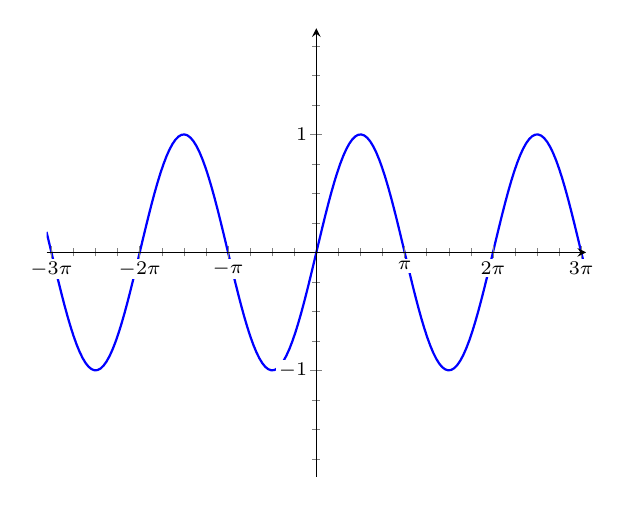
\begin{tikzpicture}
\begin{axis}[
    axis lines = middle,
    axis on top,
    minor tick num=3,
    ticklabel style={fill=white,font=\scriptsize, inner sep=1pt},
    xmin=-550, xmax=550,
    xtick={-540,-360,-180, 0, 180, 360, 540},
    xticklabels={$-3\pi$ ,$-2\pi$, $-\pi$, 0, $\pi$, $2\pi$,$3\pi$},
    ymin=-1.9, ymax=1.9,
    ytick={-2,-1,...,2},
    domain=-550:550,
    samples=181,
    no marks]         
\addplot +[blue,thick] {sin(x)};
\end{axis}
    \end{tikzpicture}}
    \end{minipage}
    
    
    
    &
    
    
     %%%%%%%%%%
     %csc
 \begin{minipage}{0.3\textwidth}
\scalebox{.95}{  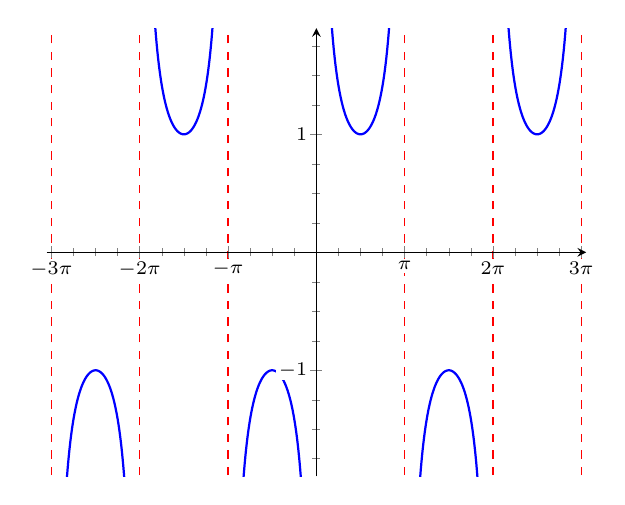
\begin{tikzpicture}
\begin{axis}[
    axis lines = middle,
    axis on top,
    minor tick num=3,
    ticklabel style={fill=white,font=\scriptsize, inner sep=1pt},
    xmin=-550, xmax=550,
    xtick={-540,-360,-180, 0, 180, 360, 540},
    xticklabels={$-3\pi$ ,$-2\pi$, $-\pi$, 0, $\pi$, $2\pi$,$3\pi$},
    ymin=-1.9, ymax=1.9,
    ytick={-2,-1,...,2},
    domain=-550:550,
    samples=181,
    no marks
            ]
  \addplot[dashed, red] coordinates{(-540,-4) (-540,4)};
 \addplot [domain=-540:-360, blue,thick] {cosec(x)};
\addplot[dashed, red] coordinates{(-360,-4) (-360,4)};
 \addplot [domain=-360:-180, blue,thick] {cosec(x)};
 \addplot[dashed, red] coordinates{(-180,-4) (-180,4)};
 \addplot [domain=-180:0, blue,thick] {cosec(x)};
  \addplot[dashed, red] coordinates{(0,-4) (0,4)};
   \addplot [domain=0:180, blue,thick] {cosec(x)};
  \addplot[dashed, red] coordinates{(180,-4) (180,4)};
   \addplot [domain=180:360, blue,thick] {cosec(x)}; 
  \addplot[dashed, red] coordinates{(360,-4) (360,4)};
\addplot [domain=360:540, blue,thick] {cosec(x)};
 \addplot[dashed, red] coordinates{(540,-4) (540,4)};
\end{axis}
    \end{tikzpicture}}
     \end{minipage}
     
     \\
     
     $y=\sin t$ & $y=\csc t = \frac{1}{\sin t}$\\
     &\\
    
    %%%%%%%%%
     %cos
\hspace{-.75in} \begin{minipage}{0.3\textwidth}    
          \scalebox{0.95}{  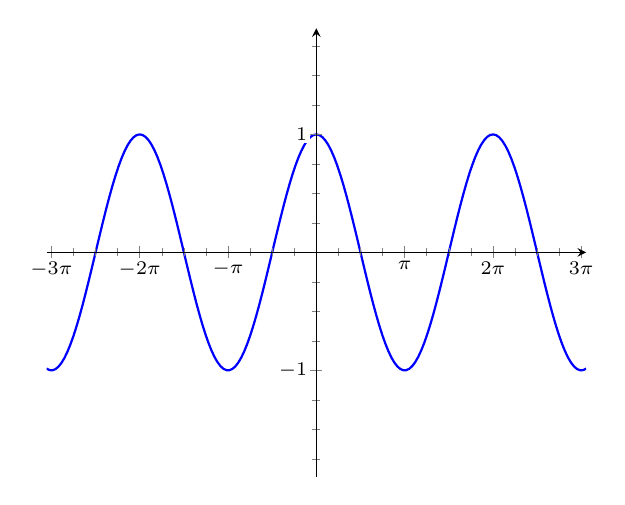
\begin{tikzpicture}
\begin{axis}[
    axis lines = middle,
    axis on top,
    minor tick num=3,
    ticklabel style={fill=white,font=\scriptsize, inner sep=1pt},
    xmin=-550, xmax=550,
    xtick={-540,-360,-180, 0, 180, 360, 540},
    xticklabels={$-3\pi$ ,$-2\pi$, $-\pi$, 0, $\pi$, $2\pi$,$3\pi$},
    ymin=-1.9, ymax=1.9,
    ytick={-2,-1,...,2},
    domain=-550:550,
    samples=181,
    no marks]
\addplot +[blue,thick] {cos(x)};
\end{axis}
    \end{tikzpicture}}
     \end{minipage}     
     
     
     
     &
     
     
%%%%%%%%%%%%%
%sec
 \begin{minipage}{0.3\textwidth}
         \scalebox{0.95}{    \begin{tikzpicture}
\begin{axis}[
    axis lines = middle,
    axis on top,
    minor tick num=3,
    ticklabel style={fill=white,font=\scriptsize, inner sep=1pt},
    xmin=-550, xmax=550,
    xtick={-540,-360,-180, 0, 180, 360, 540},
    xticklabels={$-3\pi$ ,$-2\pi$, $-\pi$, 0, $\pi$, $2\pi$,$3\pi$},
    ymin=-1.9, ymax=1.9,
    ytick={-2,-1,...,2},
    domain=-550:550,
    samples=181,
    no marks
            ]

 \addplot [domain=-550:-460, blue,thick] {sec(x+2*pi)};
  \addplot[dashed, red] coordinates{(-450,-4) (-450,4)};
 \addplot [domain=-450:-270, blue,thick] {sec(x)};
 \addplot[dashed, red] coordinates{(-270,-4) (-270,4)};
 \addplot [domain=-270:-90, blue,thick] {sec(x)};
  \addplot[dashed, red] coordinates{(-90,-4) (-90,4)};
   \addplot [domain=-90:90, blue,thick] {sec(x)}; 
  \addplot[dashed, red] coordinates{(0,-4) (0,4)};
\addplot [domain=90:270, blue,thick] {sec(x)};
 \addplot[dashed, red] coordinates{(90,-4) (90,4)};
 \addplot [domain=270:450, blue,thick] {sec(x)};
 \addplot[dashed, red] coordinates{(270,-4) (270,4)};
 \addplot [domain=450:550, blue,thick] {sec(x)};
 \addplot[dashed, red] coordinates{(450,-4) (450,4)};
\end{axis}
    \end{tikzpicture}}
     \end{minipage}
     
     
     \\
     
     
     
$y=\cos t$ & $y=\sec t = \frac{1}{\cos t}$\\
&\\
    
    %%%%%%%%%
%tan
\hspace{-.75in}\begin{minipage}{0.3\textwidth} 
      \scalebox{0.95}{   \begin{tikzpicture}
\begin{axis}[
    axis lines = middle,
    axis on top,
    minor tick num=3,
    ticklabel style={fill=white,font=\scriptsize, inner sep=1pt},
    xmin=-550, xmax=550,
    xtick={-540,-360,-180, 0, 180, 360, 540},
    xticklabels={$-3\pi$ ,$-2\pi$, $-\pi$, 0, $\pi$, $2\pi$,$3\pi$},
    ymin=-4, ymax=4,
    ytick={-4,-3,...,4},
    domain=-550:550,
    samples=181,
    no marks]
 \addplot [domain=-549:-460, blue,thick] {tan(x)};
  \addplot[dashed, red] coordinates{(-450,-4) (-450,4)};
 \addplot [domain=-450:-270, blue,thick] {tan(x)};
 \addplot[dashed, red] coordinates{(-270,-4) (-270,4)};
 \addplot [domain=-270:-90, blue,thick] {tan(x)};
  \addplot[dashed, red] coordinates{(-90,-4) (-90,4)};
   \addplot [domain=-90:90, blue,thick] {tan(x)}; 
  \addplot[dashed, red] coordinates{(0,-4) (0,4)};
\addplot [domain=90:270, blue,thick] {tan(x)};
 \addplot[dashed, red] coordinates{(90,-4) (90,4)};
 \addplot [domain=270:450, blue,thick] {tan(x)};
 \addplot[dashed, red] coordinates{(270,-4) (270,4)};
 \addplot [domain=450:550, blue,thick] {tan(x)};
 \addplot[dashed, red] coordinates{(450,-4) (450,4)};
\end{axis}
    \end{tikzpicture}}
     \end{minipage}
     
     
     
&
 
%%%%%%%%
%cot
 \begin{minipage}{0.3\textwidth}           
         \scalebox{0.95}{    \begin{tikzpicture}
\begin{axis}[
    axis lines = middle,
    axis on top,
    minor tick num=3,
    ticklabel style={fill=white,font=\scriptsize, inner sep=1pt},
    xmin=-550, xmax=550,
    xtick={-540,-360,-180, 0, 180, 360, 540},
    xticklabels={$-3\pi$ ,$-2\pi$, $-\pi$, 0, $\pi$, $2\pi$,$3\pi$},
    ymin=-1.9, ymax=1.9,
    ytick={-2,-1,...,2},
    domain=-550:550,
    samples=181,
    no marks
            ]

  \addplot[dashed, red] coordinates{(-540,-4) (-540,4)};
 \addplot [domain=-540:-360, blue,thick] {cot(x)};
\addplot[dashed, red] coordinates{(-360,-4) (-360,4)};
 \addplot [domain=-360:-180, blue,thick] {cot(x)};
 \addplot[dashed, red] coordinates{(-180,-4) (-180,4)};
 \addplot [domain=-180:0, blue,thick] {cot(x)};
  \addplot[dashed, red] coordinates{(0,-4) (0,4)};
   \addplot [domain=0:180, blue,thick] {cot(x)};
  \addplot[dashed, red] coordinates{(180,-4) (180,4)};
   \addplot [domain=180:360, blue,thick] {cot(x)}; 
  \addplot[dashed, red] coordinates{(360,-4) (360,4)};
\addplot [domain=360:540, blue,thick] {cot(x)};
 \addplot[dashed, red] coordinates{(540,-4) (540,4)};
\end{axis}
    \end{tikzpicture}}
         \end{minipage}
         
\\

$y=\tan t$ & $y=\cot t = \frac{\cos t}{\sin t}$\\

\end{longtable}


       
          

    
    
%\todo{I really wish we could just use these pictures but the vertical asymptotes for tangent are in the wrong places. It's been driving me crazy for almost 10 years. Robyn, can you tikz something that's similar to all of these?}

%\todo{Summary of domain and range for all six functions. Will probably need to discuss how to write the locations of the asymptotes using $k$'s. Also discuss period. }


We summarize some properties of the six trigonometric functions that can be seen in the graphs above:

\begin{theorem}[Domain, Range, and Period of the Six Trigonometric Functions] The six trigonometric functions $\sin t, \cos t, \tan t, \csc t, \sec t,$ and $\cot t$ have the following domain, range, and period:
\begin{itemize}[itemsep=10pt,topsep=5pt]
\item The domain of both $\sin t$ and $\cos t$ is the set of all real numbers and their range is $[-1,1]$. They are periodic with period $2\pi$. 

\item The domain of $\tan t$ is the set of all real numbers $t$ \textit{except} for odd multiples of $\pi/2$: $t\neq \ldots -\frac{3\pi}{2}, -\frac{\pi}{2}, \frac{\pi}{2}, \frac{3\pi}{2},\ldots$ and its range is $(-\infty,\infty)$. It is periodic with period $\pi$. 

\item The domain of $\csc t$ is the set of all real numbers $t$ \textit{except} for multiples of $\pi$: \\$t\neq \ldots -2\pi, -\pi, 0, \pi, 2\pi,\ldots$ and its range is $(-\infty,-1)\cup(1,\infty)$. It is periodic with period $2\pi$. 

\item The domain of $\sec t$ is the set of all real numbers $t$ \textit{except} for odd multiples of $\pi/2$: $t\neq \ldots -\frac{3\pi}{2}, -\frac{\pi}{2}, \frac{\pi}{2}, \frac{3\pi}{2},\ldots$ and its range is $(-\infty,-1)\cup(1,\infty)$. It is periodic with period $2\pi$. 

\item The domain of $\cot t$ is the set of all real numbers $t$ \textit{except} for multiples of $\pi$: \\$t\neq \ldots -2\pi, -\pi, 0, \pi, 2\pi,\ldots$ and its range is $(-\infty,-1)\cup(1,\infty)$. It is periodic with period $\pi$. 
\end{itemize}
\end{theorem}

\textit{The above properties should not be memorized}, but rather should be understood from the definitions. We have already explored how $\sin t$ and $\cos t$ are defined for all values of $t$, take on values between $-1$ and $1$ inclusive, and are periodic with period $2\pi$. These all come from their definition as the vertical/horizontal value of a point moving around the unit circle. 

The function $\tan t$ is undefined at all values of $t$ where $\cos t=0$, since we define $\tan t = \frac{\sin t}{\cos t}$. These are the angles corresponding to the vertical axis of the unit circle, so the odd multiples of $\pi/2$, which can be written
$$t = \frac{(2k+1)\pi}{2}\quad\text{where }k\text{ is a positive or negative whole number.}$$
At those points, $\tan t$ has vertical asymptotes since $\sin t = \pm1$ where $\cos t = 0$, thus $\ds\lim_{t\to (2k+1)\pi/2}\tan t$ has the form $\frac{1}{0}$. In particular, when $t\to\pi/2$, $\sin t\to 1$ and $\cos t\to 0$ from both above (when $t\to 0^-$) and below (when $t\to 0^+$), so we see that the asymptotes go to both $\infty$ and $-\infty$, so $\tan t$ has range $(-\infty,\infty)$. We cannot yet prove rigorously that $\tan t$ has period $\pi$, rather than $2\pi$, but it is clear to see from the graph, and is due to the fact that the sign of $\frac{\sin t}{\cos t}$ is positive for $t$ in the first quadrant, negative for $t$ in the second quadrant, then positive again for $t$ in the third quadrant, and negative for $t$ in the fourth quadrant. (The period of $\tan t$ will be the last thing we examine in this section.)

Let's take a closer look at the graph of $\csc t = \frac{1}{\sin t}$. It is undefined at all values of $t$ where $\sin t=0$.  These are the angles corresponding to the horizontal axis of the unit circle, which are the multiples of $\pi$, and can be written
$$t = k\pi\quad\text{where }k\text{ is a positive or negative whole number.}$$
At those points, $\csc t$ has vertical asymptotes since $\ds\lim_{t\to k\pi}\csc t$ has the form $\frac{1}{0}$, and we can see that for each such $t$, $\sin t$ approaches $0^+$ on one side and $0^-$ on the other. The range of $\csc t$ is \textit{not} all real numbers, however, since the values of $\csc t$ cannot be between $-1$ and $1$. This is because  $\sin t\leq1$ and $\sin t\geq-1$, so either $\csc t = \frac{1}{\sin t}\geq1$ or $\csc t = \frac{1}{\sin t}\leq-1$. The period of $\csc t$ is $2\pi$ because the period of $\sin t$ is $2\pi$. 

\begin{exercise}
For what values of $t$ does $\sec t$ have vertical asymptotes? How can you see this on the graph of $\cos t$? 
%Use the fact that $\sec t = \frac{1}{\cos t}$ to explain in your own words the domain, range, and period of $\sec t$. Use the fact that $\cot t = \frac{\cos t}{\sin t}$ to explain in your own words the domain and range of $\cot t$. \textit{Note that $\cot t$ has the same period, $\pi$, as $\tan t$, though we cannot explain fully why this is true yet.}
\end{exercise}








\subsection{Solving Equations Involving Trigonometric Functions}

Now that we know what the trigonometric functions look like, have a table of values that we could memorize (or look up), and have constant access to a calculator for all of the other values, it might be tempting to forget all about the unit circle definitions of sine and cosine. However, the unit circle provides a crucial perspective  that allows us to solve equations involving trigonometric functions, and also derive further useful properties of trigonometric functions. 

In the next example, we demonstrate how to use the unit circle to solve fairly basic equations involving sine and cosine.

\begin{example}
%\todo{Taalman Section 6.1 Example 5}
Find all of the solutions of the equation $\sin\theta=\cos\theta$.

\begin{solution}

If $\sin\theta=\cos\theta$, then $\theta$ is an angle whose terminal edge intersects the unit circle at a point $(x,y)$ with $x=y$, since the coordinates $(x,y)$ on the unit circle correspond to the points $(\cos\theta,\sin\theta)$.  The only such points on the unit circle are $\left(\frac{\sqrt{2}}{2},\frac{\sqrt{2}}{2}\right)$ and $\left(-\frac{\sqrt{2}}{2},-\frac{\sqrt{2}}{2}\right)$, as shown in Figure \ref{fig:TaalmanPage411} below.  

\begin{figure}[H]
\centering
\includegraphics[width=2in]{TaalmanPage411.png}
\caption{The line $y=x$ intersects the unit circle at the points  $\left(\frac{\sqrt{2}}{2},\frac{\sqrt{2}}{2}\right)$ and $\left(-\frac{\sqrt{2}}{2},-\frac{\sqrt{2}}{2}\right)$.}
\label{fig:TaalmanPage411}
\end{figure}

The angles that end at these points are all of the form $\theta=\frac{\pi}{4}+\pi k$ for some integer $k$.  Thus, the solution set for the equation is $\left\{\dots,-\frac{3\pi}{4},\frac{\pi}{4},\frac{5\pi}{4},\frac{9\pi}{4},\dots\right\}$.

\end{solution}
\end{example}

Below is another application of our understanding of the unit-circle origins of sine and cosine. We can often find the value of one function if we are given the value of another function, without having to know the precise angle involved. 


\begin{example}\label{ex:Taalman6-1-4}
%\todo{Taalman Section 6.1 Example 4}
Given that $\cos\theta=-\frac{1}{3}$ and $\theta$ is an angle that terminates in the third quadrant, find $\tan\theta$.
\begin{solution}
Since $\cos\theta=-\frac{1}{3}$, the angle $\theta$ must intersect the unit circle at a point whose $x$-coordinate is $-\frac{1}{3}$, as shown next.  Only one of these points is in the third quadrant, and it is of the form $\left(-\frac{1}{3},y\right)$ where $y$ is some negative number.

\begin{center}
\includegraphics[width=2in]{TaalmanPage410c.png}
\end{center}

To find the tangent of $\theta$, we need to know the $y$-coordinate of the point we have identified in the third quadrant.  Because the radius of the circle is 1 and is the hypotenuse of a right triangle with base $x=\frac{1}{3}$ and height $y$, by the Pythagorean Theorem, it follows that 

$$\begin{aligned}
y^2+\left(-\frac{1}{3}\right)^2 &=1 \\
y^2+\frac{1}{9}&=1\\
y &=\pm\sqrt{1-\frac{1}{9}}\\
&=\pm\sqrt{\frac{8}{9}}\\
&=\pm\frac{2\sqrt{2}}{3}.\end{aligned}$$

Since $\theta$ terminates in the third quadrant, the $y$-coordinate corresponding to $\theta$ is the negative choice:  
$$y= -\frac{2\sqrt{2}}{3}.$$  

As a reality check, $-\frac{2\sqrt{2}}{3}\approx -0.9428$ is a reasonable answer, since the point in question has a $y$ coordinate very close to $-1$.  

We can now say that 

$$\tan\theta=\frac{y}{x}=\frac{-\frac{2\sqrt{2}}{3}}{-\frac{1}{3}}=\frac{2\sqrt{2}}{1}=2\sqrt{2}.$$

It is interesting to note that we never actually had to determine the angle measure of $\theta$, we only needed to know the $(x,y)$ coordinates of the corresponding point on the unit circle.
\end{solution}
\end{example}


\begin{exercise}
Suppose as in Example \ref{ex:Taalman6-1-4} you know that $\cos\theta = -\frac{1}{3}$, but you are not told that $\theta$ is an angle that terminates in the third quadrant. What other value could $\tan\theta$ have?
\end{exercise}

\subsection{A Practical Example of Using Trigonometric Functions}

There are also many practical uses for trigonometric functions and reasons to want to solve problems like in the last section. The origins of trigonometry can be traced to the civilizations of ancient Egypt, Mesopotamia and the Indus Valley (India), more than 4000 years ago.\footnote{\href{https://www.newworldencyclopedia.org/entry/trigonometry}{https://www.newworldencyclopedia.org/entry/trigonometry}} Here is a modern application of some of these very old ideas. 

\begin{example}
%\todo{Taalman Section 6.1 Example 6}
Suppose you are 500 feet from the base of an office building, and suppose that the angle of elevation of your line of sight (i.e., the angle between the horizontal ground and your diagonal line of sight) to the top of the building is 36 degrees.  How tall is the building?
\begin{solution}

Suppose $h$ is the height of the building.  You are standing 500 feet away from the building as shown in the following diagram:


\begin{center}
\includegraphics[width=3.5in]{TaalmanPage412a.png}
\end{center}

We know the length of the side of the triangle adjacent to the 36 degree angle, and we would like to find the length of the side that is opposite that angle,  The tangent function relates those two sides, specifically, $\tan(36^{\circ})$ is the ratio of the height of the building to the distance you are from the building:

$$\tan(36^{\circ})=\frac{\textrm{opp}}{\textrm{adj}}=\frac{h}{500} \ \implies \ h=500\tan(36^{\circ}) \ \implies \ h\approx 363.27 \ \textrm{ feet.}$$

In the last step, we use a calculator to approximate $\tan(36^{\circ})\approx0.7265$.
\end{solution}
\end{example}

Some other disciplines that make regular use of trigonometric functions are architecture and carpentry, astronomy, navigation, climate science and meteorology, and image and sound processing. 



\begin{exercise}
What are a few situations in your own life where you either observe periodic behavior that could be modeled with a circular function, or where you need to make use of relationships between angles and side lengths of triangles? 
\end{exercise}







\subsection{A Few Trigonometric Identities}

%\todo{Picking up with APC Section 2.3.3 after the box with the properties.}

Another reason to remember the unit-circle definitions of sine and cosine is in establishing the many identities that these and the other trigonometric functions satisfy. An \textbf{identity} is an equation that is always true. 

\begin{example}
For example, the equation $x^2=4$ is \textit{not} an identity because it is true only for the values $x=2$ and $x=-2$. 

By contrast, the equation $3^{2x}=9^x$ is true for \textit{all} values of $x$ and thus is an identity. 
\end{example}

Because trigonometric functions are closely related to each other, there are a LOT of trigonometric identities that describe relationships between two seemingly different trigonometric expressions that are in fact equal for all relevant values of $x$. These identities will be the key to rewriting and simplifying trigonometric expressions, much like the logarithms rules of previous chapters.\footnote{Please try not to forget them as they will be on the final exam.} 

For instance, the sine and cosine of an angle $\theta$ are the $y$-coordinate and $x$-coordinates, respectively, of the point where the terminal edge of $\theta$ meets the unit circle. Since the unit circle has equation $x^2+y^2 = 1$, the quantities $x=\cos \theta$ and $y=\sin \theta$ are related by the trigonometric identity 
$$(\cos \theta)^2+(\sin \theta)^2 = 1.$$
This equation is known as a \textbf{Pythagorean Identity}, since, for acute angles, it follows from the Pythagorean Theorem as follows: If $\theta$ is an angle in a right triangle with hypotenuse $1$, then $\sin \theta = \frac{\text{opp}}{1}$ is the length of the side opposite $\theta$ and $\cos\theta = \frac{\text{adj}}{1}$ is the length of the side adjacent to $\theta$. By the Pythagorean Theorem, the sum of the squares of those lengths must be equal to the square of the hypotenuse, again giving us the identity just listed. The following Figure illustrates these two ways of obtaining that identity:


\begin{figure}[H]
\centering
\includegraphics[width=5.5in]{TaalmanPage417.png}
\caption{Two different ways to derive the Pythagorean Identity, either via the unit-circle definition or the right-triangle definition.}
\label{fig:TaalmanPage417}
\end{figure}

For notational convenience, people often use the abbreviation 
$$\sin^2\theta\quad\text{or}\quad \cos^2\theta$$
to represent $(\sin \theta)^2$ or $(\cos\theta)^2$, respectively. We will use exponents similarly for the other trigonometric functions and for higher integer powers. 

Thus the Pythagorean Identity is typically written
$$\cos^2 \theta+\sin^2 \theta = 1.$$

\begin{remark}
The notation $\sin^2\theta\quad\text{or}\quad \cos^2\theta$ \textbf{should not } be taken to mean $\sin(\sin(\theta))$ or $\cos(\cos(\theta))$. This is confusing and I apologize on behalf of the mathematical community. 
\end{remark}

From the preceding discussion, we get the following three trigonometric identities:

\begin{theorem}[Pythagorean Identities]\label{thm:pythagidentity}
For every angle $\theta$ for which the expressions that follow are defined, 
\begin{enumerate}[label=\alph*),itemsep=5pt]
\item $\sin^2\theta+\cos^2\theta = 1$
\item $\tan^2\theta+1 = \sec^2\theta$
\item $1+\cot^2\theta = \csc^2\theta$
\end{enumerate}
\end{theorem}

\begin{proof}
We have already proved (a). To prove (b), we simply divide both sides of (a) by $\cos^2\theta$ and then simplify:
$$\begin{aligned}
\sin^2\theta +\cos^2\theta &= 1\\
\frac{\sin^2\theta +\cos^2\theta}{\cos^2\theta} &= \frac{1}{\cos^2\theta}\\
\frac{\sin^2\theta}{\cos^2\theta} +\frac{\cos^2\theta}{\cos^2\theta} &= \frac{1^2}{\cos^2\theta}\\
\left(\frac{\sin\theta}{\cos\theta}\right)^2+1 &= \left(\frac{1}{\cos\theta}\right)^2\\
\tan^2\theta +1 &=\sec^2\theta
\end{aligned}$$
\end{proof}

\begin{exercise}
Use the Pythagorean Identity (part (a) of Theorem \ref{thm:pythagidentity}) to prove the identity in part (c). \textit{Hint: Divide by a suitable trigonometric expression. }
\end{exercise}



As another example, from the unit circle we can determine that each of the six trigonometric function is either an even function or an odd function. Recall that a function $f(x)$ is \textit{even} if $f(-x) = f(x)$ for all $x$ in its domain and \textit{odd} if $f(-x) = -f(x)$. Graphs of odd functions have $180^\circ$ rotational symmetry about the origin, while graphs of even functions have reflectional symmetry across the $y$-axis. The following theorem tells us that  sine and tangent  are odd functions while the cosine function is even. 

\begin{theorem}[Even and Odd Identities]\label{thm:evenoddidentity}
For every angle $\theta$, 
\begin{enumerate}[label=\alph*),itemsep=10pt,topsep=5pt]
\item $\sin(-\theta) = -\sin\theta$
\item $\cos(-\theta) = \cos\theta$
\item $\tan(-\theta) = -\tan\theta$
\end{enumerate}
\end{theorem}

We can easily see from the graphs of $\sin t, \cos t, $ and $\tan t$ that  sine and  tangent have odd (rotational) symmetry while the cosine has even (reflection) symmetry, as shown in the next three pictures. 

\setlength{\tabcolsep}{.75in}
\renewcommand{\arraystretch}{2}
\begin{longtable}{c}
%%%%%%%
     %sin
\hspace{-.75in} \begin{minipage}{0.3\textwidth}  
\scalebox{.95}{\begin{tikzpicture}
\begin{axis}[
    axis lines = middle,
    axis on top,
    minor tick num=3,
    ticklabel style={fill=white,font=\scriptsize, inner sep=1pt},
    xmin=-550, xmax=550,
    xtick={-540,-360,-180, 0, 180, 360, 540},
    xticklabels={$-3\pi$ ,$-2\pi$, $-\pi$, 0, $\pi$, $2\pi$,$3\pi$},
    ymin=-1.9, ymax=1.9,
    ytick={-2,-1,...,2},
    domain=-550:550,
    samples=181,
    no marks]         
\addplot +[blue,thick] {sin(x)};
\end{axis}
    \end{tikzpicture}}
    \end{minipage}
    
\\

$\sin t$ is odd and has $180^\circ$ rotational symmetry about the origin\\
    
    
        %%%%%%%%%
     %cos
\hspace{-.75in} \begin{minipage}{0.3\textwidth}    
          \scalebox{0.95}{  \begin{tikzpicture}
\begin{axis}[
    axis lines = middle,
    axis on top,
    minor tick num=3,
    ticklabel style={fill=white,font=\scriptsize, inner sep=1pt},
    xmin=-550, xmax=550,
    xtick={-540,-360,-180, 0, 180, 360, 540},
    xticklabels={$-3\pi$ ,$-2\pi$, $-\pi$, 0, $\pi$, $2\pi$,$3\pi$},
    ymin=-1.9, ymax=1.9,
    ytick={-2,-1,...,2},
    domain=-550:550,
    samples=181,
    no marks]
\addplot +[blue,thick] {cos(x)};
\end{axis}
    \end{tikzpicture}}
     \end{minipage}     
     
     
     \\
     $\cos t$ is even and has reflectional symmetry across the vertical axis\\
     
    \\
     
         %%%%%%%%%
%tan
\hspace{-.75in}\begin{minipage}{0.3\textwidth} 
      \scalebox{0.95}{   \begin{tikzpicture}
\begin{axis}[
    axis lines = middle,
    axis on top,
    minor tick num=3,
    ticklabel style={fill=white,font=\scriptsize, inner sep=1pt},
    xmin=-550, xmax=550,
    xtick={-540,-360,-180, 0, 180, 360, 540},
    xticklabels={$-3\pi$ ,$-2\pi$, $-\pi$, 0, $\pi$, $2\pi$,$3\pi$},
    ymin=-4, ymax=4,
    ytick={-4,-3,...,4},
    domain=-550:550,
    samples=181,
    no marks]
 \addplot [domain=-549:-460, blue,thick] {tan(x)};
  \addplot[dashed, red] coordinates{(-450,-4) (-450,4)};
 \addplot [domain=-450:-270, blue,thick] {tan(x)};
 \addplot[dashed, red] coordinates{(-270,-4) (-270,4)};
 \addplot [domain=-270:-90, blue,thick] {tan(x)};
  \addplot[dashed, red] coordinates{(-90,-4) (-90,4)};
   \addplot [domain=-90:90, blue,thick] {tan(x)}; 
  \addplot[dashed, red] coordinates{(0,-4) (0,4)};
\addplot [domain=90:270, blue,thick] {tan(x)};
 \addplot[dashed, red] coordinates{(90,-4) (90,4)};
 \addplot [domain=270:450, blue,thick] {tan(x)};
 \addplot[dashed, red] coordinates{(270,-4) (270,4)};
 \addplot [domain=450:550, blue,thick] {tan(x)};
 \addplot[dashed, red] coordinates{(450,-4) (450,4)};
\end{axis}
    \end{tikzpicture}}
     \end{minipage}
     
     \\
     
     $\tan t$ is odd and has $180^\circ$ rotational symmetry about the origin
     
\end{longtable}


We prove these symmetries by using the unit-circle definitions of these functions. 

\begin{proof}

We'll prove part (a) and leave you to think about how to prove parts (b) and (c). Given any angle $\theta$ in standard position, the angle $-\theta$ opens up by the same angle measure, but in the opposite direction, as shown in Figure \ref{fig:TaalmanPage418a} below. 


\begin{figure}[H]
\centering
\includegraphics[width=2in]{TaalmanPage418a.png}
\caption{The $y$-coordinate corresponding to the terminal edge of $-\theta$ is the negative of the $y$-coordinate corresponding to the terminal edge of $\theta$.}
\label{fig:TaalmanPage418a}
\end{figure}

This means that if $(x,y)$ is the point on the unit circle corresponding to $\theta$, then the point $(x,-y)$ is the point on the unit circle corresponding to $-\theta$. 

Since $\sin\theta$ is the $y$-coordinate of the point at which the terminal edge of $\theta$ meets the unit circle, and $\sin(-\theta)$ is the corresponding $y$-coordinate for $-\theta$, we have shown that $\sin(-\theta) = -\sin\theta$. 

In other words, we can tell from the picture above that the $y$-coordinate of one point is the negative of the $y$-coordinate of the other point because of the symmetry of the circle.

This identity means that $y=\sin\theta$ is an odd function, which is seen in the $180^\circ$ rotational symmetry about the origin of the graph of $y=\sin t$. 
\end{proof}

\begin{exercise}
Use the same picture of the unit circle in the proof of Theorem \ref{thm:evenoddidentity} part (a) to prove part (b): $\cos(-\theta) = \cos(\theta)$. 
\end{exercise}

\begin{example}
Determine algebraically whether the function
$$f(t) = \frac{\sin t}{1+\cos t}$$
is even, odd, or neither.
\end{example}

\begin{solution}
The function $f(t)$ is even only if $f(-t) = f(t)$ and is odd only if $f(-t) = -f(t)$. If neither of these identities are true, then the function is neither even nor odd. 

Let's see what we can say about $f(-t) = \frac{\sin(-t)}{1+\cos(-t)}$. We know that $\sin(-t) = -\sin t$ and that $\cos(-t) = \cos t$ are identities, so this tells us that
$$f(-t) = \frac{\sin(-t)}{1+\cos(-t)} = \frac{-\sin t}{1+\cos t} = -\left(\frac{\sin t}{1+\cos t} \right)= -f(t).$$
Since we have $f(-t) = -f(t)$, we can see that $f(t)$ is an odd function. 
\end{solution}

We will prove part (c) in class: that $\tan t$ is an odd function.


%\begin{exercise}
%Use the even and odd identities for $\sin t$ and $\cos t$ to prove that
%$$f(t) = \tan t = \frac{\sin t}{\cos t}$$
%is odd. 
%\end{exercise}

%\todo{Taalman Section 6.2 through the first two sections (only do the Pythagorean identity with sin and cos for now, or maybe have students do the others as exercises?). Also example 2, example 3 (modified; don't find angles for which it's true)}

We can quickly obtain one more identity by further examining the unit-circle definition of the trigonometric functions. 

\begin{example}
For example, for every angle $\theta$ we clearly have $$\sin (\theta+2\pi) = \sin\theta,$$ since $\theta+2\pi$ and $\theta$ have the same terminal edge and thus intersect the unit circle at the same point. This is the same as observing that the function $\sin \theta$ has period $2\pi$. Likewise, we have
$$\cos(\theta+2\pi) = \cos\theta.$$
\end{example}


Lest we forget the graphs with which we started this section, let's return to them and use them to justify a few more identities. If we juxtapose the sine and cosine functions' graphs on the same coordinate axes, as seen in Figure \ref{fig:APCFigure2-3-12} below, we see that the curves can be viewed as horizontal translations of one another.

\begin{figure}[H]
\centering
\includegraphics[width=3.5in]{APCFigure2-3-12.png}
\caption{The graph of $f(t) = \sin t$ is the graph of $g(t) = \cos t$ shifted to the right $\pi/2$ units.}
\label{fig:APCFigure2-3-12}
\end{figure}


In particular, since the sine graph can be viewed as the cosine graph shifted $\frac{\pi}{2}$ units to the right, it follows that for any value of $t$, 
$$\sin t = \cos (t-\frac{\pi}{2}).$$
Similarly, since the cosine graph can be viewed as the sine graph shifted left $\frac{\pi}{2}$ units, 
$$\cos t = \sin (t+\frac{\pi}{2}).$$


We can also see that if we shift the graph of sine $\pi$ units to the right or left, the result is the reflection of the graph of sine across the horizontal axis. See Figure \ref{fig:SineShiftByPi} below. 

\begin{figure}[H]
\centering
\includegraphics[width=2.5in]{SineShiftByPi.png}
\caption{The graph of $y=\sin(t\pm \pi)$ is the graph of $y=\sin t$ reflected over the $x$-axis.}
\label{fig:SineShiftByPi}
\end{figure}

The same is true for the graph of $\cos t$. This tells us that
$$ \sin (t+\pi) = \sin(t-\pi) = -\sin t $$
and
$$\cos(t+\pi) = \cos(t-\pi) = -\cos t.$$
. 



These identities allow us to observe, finally, why it is that $\tan t$ has period $\pi$. For all $t$, 
$$\tan(t+\pi) = \frac{\sin(t+\pi)}{\cos(t+\pi)} = \frac{-\sin t}{-\cos t} = \frac{\sin t}{\cos t} = \tan t.$$

\begin{exercise}
Skim through this last section and write down all of the trigonometric identities listed.
\end{exercise}




\subsection*{Summary}
The following terms and theorems were introduced in this section: 
\begin{quotation}
Identity, Pythagorean Identities, even and odd identities
\end{quotation}

\textbf{Key ideas:} The shapes of the graphs of the six trigonometric functions follow from their definitions. It is not worth memorizing the numerous properties of these functions, but rather understanding where they come from and re-deriving them from a small collection of basic principles when necessary. The unit-circle definition is particularly useful to keep in mind for solving equations involving trigonometric functions, and in remembering identities involving the trigonometric functions.

\textbf{Other ideas introduced:} There are many relationships between the various trigonometric functions that allow us to simplify expressions in order to more easily solve problems. 




\begin{center}
\textcolor{ocre}{\fbox{\fbox{\Large \bf \sc End of Section 7.3}}}
\end{center}

\hspace{-.5in}\rule{1.1\textwidth}{2pt}











%----------------------------------------------------------------------------------------
%	Section 4
%----------------------------------------------------------------------------------------






\section{Defining Inverse Trigonometric Functions}


\subsection*{Learning Goals}

\begin{itemize}
	\item Recall that functions must be one-to-one in order to have an inverse. As a result, we must restrict the domains of the trigonometric functions in order to define their (partial) inverse functions. 
	\item Define the inverse functions arccosine, arcsine, and arctangent, and determine their domains and ranges. 
	\item Practice calculating values of inverse trigonometric functions, and learn what common mistakes to avoid while doing so. 
\end{itemize}


\subsection{A Brief Recap of Inverse Functions}



Recall from Section \ref{sec:inversefunctions} that a function has an inverse only if the function is one-to-one, or in other words that it passes the Horizontal Line Test. This allows us to "reverse" a function $y=f(x)$ to obtain a function $f^{-1}(y) = x$. 

\begin{example}
For example, if $f(x) = x^3$, then $f^{-1}(y) = \sqrt[3]{y}$. 
\end{example}

\begin{example}
For another example, if $f(x) = e^x$, then $f^{-1}(y) = \ln y$. 
\end{example}


Given a one-to-one function $f(x)$, its inverse is by definition the function $f^{-1}(x)$ with the property that
$$f^{-1}(f(x)) = x\quad\text{and}\quad f(f^{-1}(y)) = y$$
for all $x$ in the domain of $f$ and for all $y$ in the domain of $f^{-1}$. 

\begin{example}
For $f(x) = x^3$, we have
$$f^{-1}(f(x)) = \sqrt[3]{x^3} = x,\quad\text{for all real numbers }x$$
$$f(f^{-1}(y)) = (\sqrt[3]{y})^3 = y,\quad\text{for all real numbers }y$$
\end{example}


\begin{example}
For $f(x) = e^x$, we have
$$f^{-1}(f(x)) = \ln(e^x) = x,\quad\text{for all real numbers }x$$
$$f(f^{-1}(y)) = e^{\ln y} = y,\quad\text{for all positive real numbers }y$$
\end{example}

If a function fails to be one-to-one, then it does not have an inverse. However, we can restrict the domain on which we consider the function in order to make the remaining function one-to-one, and define an inverse of the function restricted to that domain. 

\begin{example}
For example, the function $f(x) = x^2+1$ fails the horizontal line test and therefore is not one-to one on the domain $(-\infty,\infty)$. But on the restricted domain $[0,\infty)$, the function $f(x)  = x^2+1$ is one-to-one, as we can see in Figure \ref{fig:RestrictedDomain} below:

\begin{figure}[H]
\centering
\includegraphics[width=2.5in]{RestrictedDomain.png}
\caption{The function $f(x) = x^2+1$ on the \textit{restricted} domain $[0,\infty)$ is indeed one-to-one.}
\label{fig:RestrictedDomain}
\end{figure}

From the graph  in Figure \ref{fig:RestrictedDomain} we also see that the range of $f(x)$ is $[1,\infty)$. This tells us that the domain of $f^{-1}$ is $[1,\infty)$ before we do any computations. 

A formula for the inverse for $f$ can be computed via
$$\begin{aligned}
y &= x^2+1\\
y-1 &= x^2\\
\pm\sqrt{y-1} &= x
\end{aligned}$$
It seems that we have \textit{two} formulas for $f^{-1}$, consisting of $\sqrt{y-1}$ and $-\sqrt{y-1}$. However, since we have restricted the domain for $x$ to $x\geq 0$, we only want the positive square root and can write 
$$x = f^{-1}(y) = \sqrt{y-1}$$
Now we can verify explicitly that the domain of $f^{-1}$ is the range $[1,\infty)$ of $f$, since we need $y-1\geq 0$ within the square root, meaning that $y\geq 1$. 

Let's check our work both algebraically and geometrically:

We can check that the definition of an inverse function is satisfied by simplifying the compositions $f\circ f^{-1}$ and $f^{-1}\circ f$:
$$f^{-1}(f(x)) = \sqrt{(x^2+1)-1} = \sqrt{x^2} = x,\quad\text{for all }x\geq 0$$
$$f(f^{-1}(y)) = (\sqrt{y-1})^2+1 = (y-1)+1 = y,\quad\text{for all }y\geq 1$$

Visually, we see that the graph of $f^{-1}(x) = \sqrt{x-1}$ is the graph of $f(x)$ reflected over the line $y=x$:

\begin{figure}[H]
\centering
\includegraphics[width=2.5in]{RestrictedDomainAndInverse.png}
\caption{$f(x)$ (in blue) on the restricted domain $[0,\infty)$ and its inverse $f^{-1}(x)$ (in green).}
\end{figure}

\end{example}


In the rest of this section, we discuss inverses of the trigonometric functions. There is a rather significant obstacle to this: none of them are one-to-one. 

The function $y=\sin \theta$ takes angles as inputs and returns $y$-coordinates on the unit circle as outputs. Is there a way to reverse this function to an inverse function $\sin^{-1}y = \theta$ that takes $y$-coordinates on the unit circle as inputs and returns angles as outputs? Not immediately, since $\sin \theta$ is not one-to-one: many angles correspond to any given $y$-coordinate on the unit circle. 

In fact, \textit{none} of the six trigonometric functions are one-to-one, but after restricting domains we can construct the so-called inverse trigonometric functions. In this section, we will focus on the inverse of only three of the six inverse trigonometric functions: Those for cosine, sine, and tangent. 

\begin{exercise}
Give three examples of angles $\theta$ for which $\sin\theta = 1$. This shows us that we cannot "reverse" the function sine without restricting its domain. 
\end{exercise}

\subsection{The arccosine function}
The function cosine repeats itself over and over and over again, so there are many different intervals we could use to define an inverse. The important part is that we pick one domain and stick to it consistently. %There are many different restricted domains that we could use to obtain partial inverses to these three functions. We need to pick one restricted domain for each function and stick with it. 

Consider the plot of the standard cosine function in Figure \ref{fig:APCFigure4-3-1} below along with the emphasized portion of the graph on $[0,\pi]$. 

\begin{figure}[H]
\centering
\includegraphics[width=4.5in]{APCFigure4-3-1.png}
\caption{$y = \cos t$ is one-to-one on the interval $[0,\pi]$.}
\label{fig:APCFigure4-3-1}
\end{figure}

If we consider  $g(t) = \cos t$ for only $0\leq t\leq \pi$, then the domain of $g(t)$ is the interval $[0,\pi]$, but its range is still $[-1,1]$, the entire range of the cosine function. Since $g$ is decreasing on its domain, we can see that it passes the Horizontal Line Test. Thus $g$ has an inverse function, and before computing anything we know that the inverse $g^{-1}$ has domain $[-1,1]$ and range $[0,\pi]$. Note that $g$ is defined in terms of the cosine function, but because it has a different domain, it is \textit{not} the cosine function. This restricted version of the cosine function has an inverse function, which we call the \textbf{arccosine} function. 

\begin{definition}
For any real number $x$ that satisfies $-1\leq x\leq 1$, the \textbf{arccosine of $x$}, denoted
$$\arccos(x) = \cos^{-1}(x)$$
is the angle $\theta$ satisfying $0\leq \theta\leq \pi$ such that $\cos(\theta) = x$. 
\end{definition}

Note particularly that the \textit{output} of the arccosine function is an angle. In addition, recall that in the context of the unit circle, an angle measured in radians and the corresponding arc length along the unit circle are numerically equal. This is why we use the "arc" in "arccosine": given a value $1\leq x\leq 1$, the arccosine function produces the corresponding \textit{arc} (measured counterclockwise from $(1,0)$), such that the cosine of that arc is $x$. 



Below we see that graph of $y=\cos t$ restricted to the domain $[0,\pi]$ (in light blue) along with the graph of the arccosine function $y=\arccos t$ (in dark blue), plotted on the same axis. (If you ask me, the graph of arccosine is not particularly enlightening and not worth remembering, but here it is anyway.)


\begin{figure}[H]
\centering
\includegraphics[width=2in]{APCarccosgraph.png}
\caption{The graph of $y=\arccos t$ (dark blue) is the graph of $y=\cos t$ restricted to $0\leq t\leq \pi$ (light blue) reflected over $y=t$. }
\label{fig:APCarccosgraph}
\end{figure}

Just as the natural logarithm function allowed us to rewrite exponential equations in an equivalent way, the arccosine function allows us to do likewise for certain angles and cosine outputs. 

\begin{example}
For instance, saying $\cos(\frac{\pi}{2}) = 0$ is the same as writing $\frac{\pi}{2} = \arccos(0)$, which reads "$\frac{\pi}{2}$ is the angle whose cosine is $0$". 
\end{example}

Indeed, these relationships are reflected in the plot in Figure \ref{fig:APCarccosgraph} above, where we see that any point $(a,b)$ that lies on the graph of $y=\cos t$ corresponds to the point $(b,a)$ that lies on the graph of $y=\arccos t$. 


\begin{exercise}
We know that $\cos(\frac{\pi}{4}) = \frac{\sqrt{2}}{2}$. What is the exact value of $\arccos(\frac{\sqrt{2}}{2})$? How about the exact value of $\arccos(-\frac{\sqrt{2}}{2})$? \textit{Recall: the range of $\arccos(x)$ is $[0,\pi]$, meaning that  your answer should be an angle (in radian measure) between $0$ and $\pi$.}
\end{exercise}

\noindent
\fbox{\parbox{6in}{
There are two equivalent notations for all of the inverse trigonometric functions. 
$$\arccos x\quad\text{and}\quad \cos^{-1} x$$
mean the exact same thing: the inverse function of $\cos \theta$ restricted to the domain $0\leq \theta\leq \pi$. You will see the two notations used interchangeably, both here and in other sources. 
}}

\subsection{The arcsine function}

We can develop an inverse function for a restricted version of the sine function in a similar way. As with the cosine function, we need to choose an interval on which the sine function is always increasing or always decreasing in order to have the function pass the Horizontal Line Test. The standard choice is the domain $[-\frac{\pi}{2},\frac{\pi}{2}]$ on which $f(t) = \sin t$ is increasing and attains all of the values in the range of the sine function. Thus we consider $f(t) = \sin t$ with domain $[-\frac{\pi}{2},\frac{\pi}{2}]$ and range $[-1,1]$ and hence define the corresponding arcsine function. 

\begin{definition}
For any real number $x$ that satisfies $-1\leq x\leq 1$, the \textbf{arcsine of $x$}, denoted
$$\arcsin(x) = \sin^{-1}(x)$$
is the angle $\theta$ satisfying $-\frac{\pi}{2}\leq \theta\leq \frac{\pi}{2}$ such that $\sin(\theta) = x$. 
\end{definition}
 The graphs of $y=\sin x$ restricted to $[-\frac{\pi}{2},\frac{\pi}{2}]$ and $y=\arcsin x$ appear below. Note that the domain of the arcsine function is $[-1,1]$ and its range is $[-\frac{\pi}{2},\frac{\pi}{2}]$. 
 
 

 
 \begin{figure}[H]
	\centering
	\begin{subfigure}[H]{0.4\textwidth}
    		\centering
    		\includegraphics[width=0.7\textwidth]{TaalmanPage438a.png}
    		\caption{$y=\sin x$ restricted to the domain $[-\frac{\pi}{2},\frac{\pi}{2}]$.}
    		\label{fig:TaalmanPage438a}
	\end{subfigure}
	\hspace{.5in}
	\begin{subfigure}[H]{0.4\textwidth}
		\centering
		\includegraphics[width=0.7\textwidth]{TaalmanPage439a.png}
		\caption{$y=\sin^{-1}x$.}
		\label{fig:TaalmanPage439a}
	\end{subfigure}
\caption{The graph of $y=\sin x$ on the restricted domain $[-\frac{\pi}{2},\frac{\pi}{2}]$ (left) and the graph of $y=\sin^{-1}x$ (right).}
\label{fig:TaalmanPage439}
\end{figure}
 
 \begin{example}
 We can calculate the exact value of $ \sin^{-1}\left(\frac{1}{2}\right)$ using the unit circle. First, we translate from inverse trigonometric function to trigonometric function:
 $$\theta = \sin^{-1}\left(\frac{1}{2}\right) \qquad \Longleftrightarrow\qquad \sin\theta = \frac{1}{2}\quad\text{ with } -\frac{\pi}{2}\leq \theta\leq \frac{\pi}{2}$$
 
 There are infinitely many angles whose sine is $\frac{1}{2}$; recall that this means the $y$-value of the point on the unit circle must be $\frac{1}{2}$. Only one of those angles is in the restricted domain $[-\frac{\pi}{2},\frac{\pi}{2}]$ shown below:
 
  \begin{figure}[H]
  \centering
 \includegraphics[width=2in]{TaalmanPage442b.png}
 \caption{The only point on the unit circle in the restricted domain $[-\frac{\pi}{2},\frac{\pi}{2}]$ with height $\frac{1}{2}$.}
 \label{fig:TaalmanPage442b}
 \end{figure}
 
 Either using a labeled picture of the unit circle and finding where sine is $\frac{1}{2}$ on this domain, or fitting a $30-60-90$ triangle into the picture as shown below, we see that the only angle meeting both of these criteria is $\theta = \frac{\pi}{6}$. 
 
\begin{figure}[H]
\centering
 \includegraphics[width=2in]{TaalmanPage442c.png}
 \caption{$\theta = \frac{\pi}{6}$ is the only angle in $[-\frac{\pi}{2},\frac{\pi}{2}]$ whose sine is equal to $\frac{1}{2}$.}
 \end{figure}
 
 Therefore $\arcsin\left(\frac{1}{2}\right) = \frac{\pi}{6}$. 
 \end{example}
 
 \begin{exercise}
 Use the labeled picture of the unit circle you created in Exercise \ref{ex:trigvaluesonunitcircle} to determine the following values exactly: $\arcsin(-1), \arcsin\left(-\frac{\sqrt{2}}{2}\right),$ and $ \arcsin(0)$. 
 
 \textit{Remember, you should have only one answer for each, the answer should be an angle, and the angle should be between $-\frac{\pi}{2}$ and $\frac{\pi}{2}$. }
 \end{exercise}
 

 There are two standard notations for the arcsin function: $\arcsin t$ and $\sin^{-1} t$. The latter reminds us that the arcsin function is the inverse of the sine function, but we must be careful about how we apply this because of the restriction on the domain of sine. 
 
\begin{example}
For example, we can compute $\sin^{-1}\left(\sin\left(-\frac{\pi}{4}\right)\right) = -\frac{\pi}{4}$ via the property $\sin^{-1}(\sin x) = x$ of inverse functions. However, this is only true because $-\frac{\pi}{4}$ is within the restricted domain $[-\frac{\pi}{2},\frac{\pi}{2}]$ used to define the arcsine function. 

By contrast, suppose we wish to simplify $\sin^{-1}\left(\sin\left(\frac{3\pi}{4}\right)\right)$. You may be tempted to say that $\sin^{-1}\left(\sin\left(\frac{3\pi}{4}\right)\right)$ is equal to $ \frac{3\pi}{4}$. However, $ \frac{3\pi}{4}$ is not in the domain of the restricted sine function. We must calculate $\sin\left(\frac{3\pi}{4}\right)$ and then evaluate the inverse sine function at that value (or otherwise translate the angle $\frac{3\pi}{4}$ to the correct angle between $-\frac{\pi}{2}$ and $\frac{\pi}{2}$. We know that $\sin\left(\frac{3\pi}{4}\right)=\frac{\sqrt{2}}{2}$, as shown next at the left. To find the value of $\sin^{-1}\left(\frac{\sqrt{2}}{2}\right)$, we must find the angle in $[-\frac{\pi}{2},\frac{\pi}{2}]$ whose sine is $\frac{\sqrt{2}}{2}$. This angle is $\frac{\pi}{4}$, as shown at the right. 

\begin{center}
\includegraphics[width=4in]{TaalmanPage444.png}
\end{center}

Therefore $\sin^{-1}\left(\sin\left(\frac{3\pi}{4}\right)\right) =\sin^{-1}\left(\frac{\sqrt{2}}{2}\right)= \frac{\pi}{4}$.

Alternately, it is completely accurate to use our knowledge of the unit-circle definition of sine as the $y$-coordinate on the unit circle to say that we would like the angle between $-\frac{\pi}{2}$ and $\frac{\pi}{2}$ with the same $y$-coordinate. For this example, we must simply reflect the point on the unit circle over the $y$-axis, and determine that the appropriate angle at that point is $\frac{\pi}{4}$. Use whatever form of this intuition you prefer. In either case, I recommend drawing a quick picture of the unit circle to help your reasoning. 
\end{example}


 \begin{exercise}
 \textbf{True or False?} $\sin^{-1}(\sin(5\pi)) = 5\pi$. Write a complete sentence to explain your reasoning. 
 \end{exercise}

\noindent
\fbox{\parbox{6in}{
Although we use the notation $\sin^2 x$ to represent $(\sin x)^2$ and the notation $x^{-1}$ to represent $\frac{1}{x}$, the notation $\sin^{-1}x$ does \textbf{not} represent $\frac{1}{\sin x}$. Inverse functions in general have nothing to do with reciprocals, despite what one might imagine from the notation.
}}
 

 
 \subsection{The arctangent function}
 
 Finally, we develop an inverse function for a restricted version of the tangent function. We choose the domain $\left(-\frac{\pi}{2},\frac{\pi}{2}\right)$ on which $y=\tan t$ is increasing and attains all of the values in the range $(-\infty,\infty)$ of the tangent function. 
 
 
 
 
  \begin{figure}[H]
	\centering
	\begin{subfigure}[H]{0.4\textwidth}
    		\centering
    		\includegraphics[width=0.7\textwidth]{TaalmanPage438b.png}
    		\caption{$y=\tan x$ restricted to the domain $(-\frac{\pi}{2},\frac{\pi}{2})$.}
    		\label{fig:TaalmanPage438b}
	\end{subfigure}
	\hspace{.5in}
	\begin{subfigure}[H]{0.4\textwidth}
		\centering
		\includegraphics[width=0.7\textwidth]{TaalmanPage439b.png}
		\caption{$y=\tan^{-1}x$.}
		\label{fig:TaalmanPage439b}
	\end{subfigure}
\caption{The graph of $y=\tan x$ on the restricted domain $(-\frac{\pi}{2},\frac{\pi}{2})$ (left) and the graph of $y=\tan^{-1}x$ (right).}
\label{fig:TaalmanPage438}
\end{figure}

\textbf{Note:} The graph of $y=\arctan x$ is the only graph of an inverse trigonometric function that is worth remembering. This is also the most useful of all of the inverse trigonometric functions, the reason for which you will learn later. 
 
Since the range of the tangent function is $(-\infty,\infty)$, this is the domain of the arctangent function. Likewise the range of the arctangent function is the restricted domain $\left(-\frac{\pi}{2},\frac{\pi}{2}\right)$ on which the tangent function is one-to-one. 
 
 \begin{definition}
For any real number $x$, the \textbf{arctangent of $x$}, denoted
$$\arctan(x) = \tan^{-1}(x)$$
is the angle $\theta$ satisfying $-\frac{\pi}{2}< \theta< \frac{\pi}{2}$ such that $\tan(\theta) = x$. 
\end{definition}


\begin{example}
Let's calculate the value of $\arctan(-\sqrt{3}) = \tan^{-1}(-\sqrt{3})$ using the unit circle. Translating to the tangent function, we need:
 $$\theta = \tan^{-1}(-\sqrt{3}) \qquad \Longleftrightarrow\qquad \tan\theta =-\sqrt{3}\quad\text{ with } -\frac{\pi}{2}< \theta< \frac{\pi}{2}$$
 In terms of sine and cosine, this means that 
 $$\frac{\sin\theta}{\cos\theta} = -\sqrt{3} \qquad \Longleftrightarrow\qquad \sin\theta = -\sqrt{3}\cos\theta$$
 We now have to think of an angle $\theta$ in the first or fourth quadrant of the unit circle whose sine is $-\sqrt{3}$ times its cosine. Since $\tan^{-1} x$ is a function, there must be only one such angle; we will try to "guess" it. 
 
Since $\tan\theta$ is negative, the angle $\theta$ must be in the fourth quadrant. Since only $30-60-90$ triangles involve $\sqrt{3}$, we must have one as our reference triangle. Lastly, with a little guess-and-check, we can determine that the triangle must be in the position shown to the right of Figure  \ref{fig:TaalmanPage442d}. From this, we conclude that the angle must be $-\frac{\pi}{3}$. 

\begin{figure}[H]
 \includegraphics[width=5in]{TaalmanPage442d.png}
 \caption{In order to have $\tan\theta = -\sqrt{3}$, we must have a $30-60-90$ reference triangle, with terminal angle $-\frac{\pi}{3}$.}
 \label{fig:TaalmanPage442d}
 \end{figure}
 
 Thus we have now shown that $\tan^{-1}(-\sqrt{3}) = -\frac{\pi}{3}$. 
 
 
 Note that it is \textbf{not correct} to say $\tan^{-1}(-\sqrt{3}) = \frac{2\pi}{3}$, even though $\tan\left(\frac{2\pi}{3}\right) = -\sqrt{3}$, since we have specifically defined the range of the arctangent function to be $\left(-\frac{\pi}{2},\frac{\pi}{2}\right)$. Thus any angle that we get as an output from $\tan^{-1}$ must be between $-\frac{\pi}{2}$ and $\frac{\pi}{2}$. 
 
 Likewise, it is \textbf{not correct} to say that $\tan^{-1}(-\sqrt{3}) = \frac{5\pi}{3}$, even though $\frac{5\pi}{3}$ and $-\frac{\pi}{3}$ intersect the unit circle at the same point. Again, the function arctangent is specifically defined so that we are using only the angles between $-\frac{\pi}{2}$ and $\frac{\pi}{2}$. 

\end{example}


 \begin{exercise}
 Use the labeled picture of the unit circle you created in Exercise \ref{ex:trigvaluesonunitcircle} to determine the following values exactly: $\arctan(0), \arctan(1),$ and $\arctan(-1)$. 
 
 \textit{Remember that $\tan\theta = \frac{\sin\theta}{\cos\theta}$ and that your answer should be an angle between $-\frac{\pi}{2}$ and $\frac{\pi}{2}$. }
 \end{exercise}


\noindent
We summarize the domains and ranges of the functions defined in this section:

\noindent
\fbox{\parbox{6in}{
\textbf{Domains and Ranges for Arccosine, Arcsine, and Arctangent:}

\begin{itemize}[itemsep=10pt,topsep=5pt]

\item $\arccos x  = \cos^{-1} x$ has domain $[-1,1]$ and range $\left[0,\pi\right]$. 

\item $\arcsin x  = \sin^{-1} x$ has domain $[-1,1]$ and range $\left[-\frac{\pi}{2},\frac{\pi}{2}\right]$. 

\item $\arctan x  = \tan^{-1} x$ has domain $(-\infty,\infty)$ and range $\left(-\frac{\pi}{2},\frac{\pi}{2}\right)$. 
\end{itemize}
}}







\subsection*{Summary}
The following functions were introduced in this section: 
\begin{quotation}
The arccosine function: $\arccos x = \cos^{-1}$, the arcsine function: $\arcsin x = \sin^{-1}x$, and the arctangent function: $\arctan x = \tan^{-1}x$. 
\end{quotation}

\textbf{Key ideas:} Each of the inverse trigonometric functions arises from taking a restricted domain of the corresponding trigonometric function on which the latter is one-to-one. Take particular care that the output of any inverse trigonometric function is within these restricted intervals. Inverse functions "reverse" the original function, but in this case we only have "partial" inverse functions, so it's more complicated. 

\textbf{Other ideas reinforced:}  The notation $f^{-1}$ does NOT mean $\frac{1}{f}$. 




\begin{center}
\textcolor{ocre}{\fbox{\fbox{\Large \bf \sc End of Section 7.4}}}
\end{center}

\hspace{-.5in}\rule{1.1\textwidth}{2pt}











%----------------------------------------------------------------------------------------
%	Section 5
%----------------------------------------------------------------------------------------






\section{Trigonometric Identities and Formulas}


\subsection*{Learning Goals}

\begin{itemize}
	\item Simplify compositions of trigonometric and inverse trigonometric functions into algebraic expressions. 
	\item Apply the sum and difference identities to finding the exact values of $\sin\frac{\pi}{12}$ and $\cos\frac{\pi}{12}$. 
	\item Combine the sum and difference identities into the double-angle identities. 
\end{itemize}


\subsection{Overview: A Few More Identities}


We have seen over the past few sections that there are many relationships between the trigonometric functions and that these give rise to many ways of rewriting one function in terms of another function. Likewise, there are additional relationships between the trigonometric and inverse trigonometric functions, since the latter are derived from the former. In this section, we cover a few more of these relationships, called \textit{identities}, that are the last ones we will examine this semester. 

We begin by showing how compositions of trigonometric and inverse trigonometric functions can be simplified to purely algebraic expressions, which is either surprising or not (you can decide). The second subsection gives the sum and difference identities for sine and cosine, which gives us a way to calculate the values of the trigonometric functions for $\frac{\pi}{12}$ exactly (remember how there were more points on the unit circle back in Section \ref{sec:theunitcircle} that we never labeled?). Lastly, we will combine the sum and Pythagorean Identities into what are called \textit{Double-Angle Identities,} which are some of the standard, useful trigonometric identities that you may need to use in future math classes or elsewhere. 

It's worth noting that there are an \textit{unlimited number} of trigonometric identities, and that thousands of them have been "discovered" and recorded in some book or other over the centuries during which humanity has studied trigonometry. The most useful approach that I have found to them, however, is to know that they are out there, somewhere, and that Google is extremely good at finding the ones I need in any given situation. The useful skill is not in memorizing the identities, but in recognizing which ones are applicable to a given problem. 

\subsection{Simplifying compositions of inverse trigonometric and trigonometric functions}\label{sec:simplifyingcompositionsoftrigandinversetrig}

Recall that if we know the value of, say, $\sin\theta$ and the sign of $\cos\theta$, then we can determine the value of $\cos\theta$ without knowing the precise value of the angle $\theta$. In this way, we can think of the composition 
$$\cos(\sin^{-1} x)$$
as a single function that takes as input the value $x=\sin\theta$ and gives as output the value of $\cos\theta$, with the additional condition that $\theta$ must be on the interval $\left[-\frac{\pi}{2},\frac{\pi}{2}\right]$ (because this is the range of the function $\sin^{-1}x = \arcsin x$). It follows that, if $-\frac{\pi}{2}\leq\theta\leq\frac{\pi}{2}$, then $\theta$ is in the fourth or first quadrant on the unit circle, so the value of cosine, the horizontal coordinate, is positive. The conclusion is that $\cos(\sin^{-1} x)$ must be \textit{positive}. 

It turns out that this composition can be written as an \textit{algebraic} function, meaning a function without any trigonometric or inverse trigonometric functions. Once again, we have the Pythagorean Theorem to thank for this amazing occurrance. 

\begin{example}\label{ex:compoftrigandinvtrig}
Write $\cos(\sin^{-1}x)$ as an algebraic function, that is, a function that involves only arithmetic operations and rational powers. 

The first thing we do is to define $\theta = \sin^{-1}x$, so that we can write $\sin\theta = x$ where $\theta$ must be in the interval $\left[-\frac{\pi}{2},\frac{\pi}{2}\right]$. If  we draw $\theta$ in the first quadrant $\left[0,\frac{\pi}{2}\right]$, then we can draw a reference triangle for $\theta$ as shown in Figure \ref{fig:TaalmanPage446a} below. 

\begin{figure}[H]
\centering
\includegraphics[width=2in]{TaalmanPage446a.png}
\caption{A reference triangle for an angle $\theta$ in $\left[0,\frac{\pi}{2}\right]$.}
\label{fig:TaalmanPage446a}
\end{figure} 

If we wish $\theta$ to have a sine of $x$, then the ratio of the length of the opposite side to the length of the hypotenuse must be $x$. The hypotenuse is $1$, since we are working with the unit circle, so the ratio we want is $\frac{\text{opp}}{\text{hyp}} = \frac{x}{1}$. Thus we can label the vertical leg of the triangle with $x$, the hypotenuse with $1$, and use the Pythagorean Theorem to solve for the third side:


\begin{figure}[H]
\centering
\includegraphics[width=2in]{TaalmanPage446b.png}
\caption{Use the Pythagorean Theorem to determine the length of the remaining leg.}
\label{fig:TaalmanPage446b}
\end{figure} 

Now $\cos\theta$ is the horizontal coordinate of the point on the unit circle corresponding to $\theta$, or, in terms of "adjacent over hypotenuse," we have
$$\cos\theta = \frac{\sqrt{1-x^2}}{1} = \sqrt{1-x^2}.$$

The case where $\theta$ is in the fourth quadrant, that is, where $\theta$ is in $\left[-\frac{\pi}{2},0\right]$, is similar and also shows that $\cos\theta = \sqrt{1-x^2}$. Therefore we have shown that 
$$\cos(\sin^{-1}x) = \sqrt{1-x^2}.$$
\end{example}


\begin{exercise}
Draw an alternate picture of the unit circle for Example \ref{ex:compoftrigandinvtrig} where $\theta$ is in the fourth quadrant $\left[-\frac{\pi}{2},0\right]$ and explain why the equation 
$$\cos\theta = \sqrt{1-x^2}$$
is still true, including especially why we only consider the positive square root. 
\end{exercise}

\begin{example}[Testing Values]
To verify the remarkable fact that $\cos(\sin^{-1}x) = \sqrt{1-x^2}$, we evaluate both sides at some simple $x$-values. While looking at just a few $x$-values will not prove that the two expressions are equal for all $x$, it will at least give us some evidence that the equality is reasonable. 

For example, at $x=0$ we have
$$\cos(\sin^{-1} 0) = \cos 0 = 1\quad\text{and}\quad \sqrt{1-0^2} =\sqrt{1} = 1,$$
and at $x=1$ we have
$$\cos(\sin^{-1} 1) = \cos \left(\frac{\pi}{2}\right) = 0\quad\text{and}\quad \sqrt{1-1^2} =\sqrt{0} = 0.$$

As a less trivial example, consider $x=\frac{1}{2}$. At this value we have
$$\cos\left(\sin^{-1} \left(\frac{1}{2}\right)\right) = \cos \left(\frac{\pi}{6}\right) = \frac{\sqrt{3}}{2}\quad\text{and}\quad \sqrt{1-\left(\frac{1}{2}\right)^2} =\sqrt{1-\frac{1}{4}} =\sqrt{\frac{3}{4}} =\frac{ \sqrt{3}}{2}.$$
\end{example}



\subsection{The Sum Identities}

Given two angles $\alpha$ and $\beta$, is $\sin(\alpha+\beta)$ the same thing as $\sin\alpha+\sin\beta$?  That would be convenient, but alas, it is not true.  For example, if $\alpha=\frac{\pi}{4}$ and $\beta=\frac{\pi}{2}$, then $\sin\left(\frac{\pi}{4}+\frac{\pi}{2}\right)=\sin\frac{3\pi}{4}=\frac{\sqrt{2}}{2}$, which is different from $\sin\left(\frac{\pi}{4}\right)+\sin\left(\frac{\pi}{2}\right)=\frac{\sqrt{2}}{2}+1$.  We can, however, relate the sine of the sum of two angles to the sine and cosine of those angles:


%\todo{Page 418 at the bottom only including the sum identities in the theorem, but including the "proof" of the difference identity as an example of how we can use this identity with subtraction.}

\begin{theorem}[Sum and Difference Identites]\label{thm:sumdif}
For all angles $\alpha$ and $\beta$:
\begin{enumerate}[label=\textbf{\alph*)},topsep=5pt,itemsep=10pt]
\item $\sin(\alpha-\beta)=\sin\alpha\cos\beta-\sin\beta\cos\alpha$
\item $\cos(\alpha-\beta)=\cos\alpha\cos\beta+\sin\beta\sin\alpha$
\item $\sin(\alpha+\beta)=\sin\alpha\cos\beta+\sin\beta\cos\alpha$
\item $\cos(\alpha+\beta)=\cos\alpha\cos\beta-\sin\beta\sin\alpha$
\end{enumerate}
\end{theorem}

Here is a visual proof of parts (a) and (b) --- the difference identities:

\begin{figure}[H]
\centering
\includegraphics[width=3in]{GeometricProofDifferenceIdentity.png}
\end{figure}

We won't elaborate on the visual proof, though you can feel free to stare at it for a bit and figure out what it's saying and why it works. The proofs of the sum identities follow easily from the difference identities, using the fact that sine is an odd function and cosine is an even function.  For example, we can prove part (c):
$$
\begin{aligned}
\sin(\alpha+\beta)&=\sin(\alpha-(-\beta))&\leftarrow\textrm{ rewrite sum as a difference}\\
&=\sin\alpha\cos(-\beta)-\sin(-\beta)\cos\alpha&\leftarrow\textrm{ difference identity for sine}\\
&=\sin\alpha\cos(\beta)-(-\sin(\beta))\cos\alpha&\leftarrow\textrm{ cosine is even, sine is odd}\\
&=\sin\alpha\cos\beta+\sin\beta\cos\alpha&\leftarrow\textrm{ simplify, and voil\`a!}\\
\end{aligned}
$$

\begin{example}
%\todo{Taalman Example 1}
Calculate the exact value of $\sin\frac{\pi}{12}$ by hand.
\begin{solution}
The reference triangle for $\frac{\pi}{12}$ is not a 30-60-90 triangle, nor a 45-45-90 triangle, so we cannot calculate the value of $\sin\frac{\pi}{12}$ directly.  We can, however, write $\frac{\pi}{12}$ as a difference of angles that have the desired reference triangels:

$$\frac{\pi}{12}=\frac{3\pi}{12}-\frac{2\pi}{12}=\frac{\pi}{4}-\frac{\pi}{6}.$$

By the difference identity for sine, we have
$$
\begin{aligned}
\sin\left(\frac{\pi}{12}\right)&=\sin\left(\frac{\pi}{4}-\frac{\pi}{6}\right)&\\
&=\sin\left(\frac{\pi}{4}\right)\cos\left(\frac{\pi}{6}\right)-\sin\left(\frac{\pi}{6}\right)\cos\left(\frac{\pi}{4}\right)&\leftarrow\textrm{ difference identity for sine}\\
&=\left(\frac{\sqrt{2}}{2}\right)\left(\frac{\sqrt{3}}{2}\right)-\left(\frac{1}{2}\right)\left(\frac{\sqrt{2}}{2}\right)&\leftarrow\textrm{ using reference triangles}\\
&=\frac{\sqrt{6}}{4}-\frac{\sqrt{2}}{4}&\\
&=\frac{\sqrt{6}-\sqrt{2}}{4}&\\
\end{aligned}
$$
\end{solution}
\end{example}

\begin{exercise}
Calculate the exact value of $\cos\frac{\pi}{12}$ by hand. 
\end{exercise}

Note that we are now able to label all 24 of the points on our original picture of the unit circle with exact coordinates. We will not give this as an exercise, but recommend that you take a moment to consider how you would go about this:

\begin{center}
\includegraphics[width=3.5in]{APCFigure2-2-3.png}
\end{center}

Many of the identities in Section \ref{sec:identitiespart1} are a consequence of the sum identity. 

\begin{example}
For example, we can rewrite the expression $\sin\left(t+\frac{\pi}{2}\right)$:

$$
\begin{aligned}
\sin\left(t+\frac{\pi}{2}\right)&=\sin t\cdot\cos\left(\frac{\pi}{2}\right)+\sin\left(\frac{\pi}{2}\right)\cos t\\
&=\sin t\cdot 0+1\cdot\cos t\\
&=\cos t.\\
\end{aligned}
$$

Isn't that cool?!
%\todo{finish example, ending with $\cos t$. }
\end{example}

\begin{example}
As another example, we can rewrite the expression $\cos(t-\pi)$:

%todo{finish example, ending with $-\cos t$. }
$$
\begin{aligned}
\cos\left(t-\pi\right)&=\cos t\cdot\cos\pi+\sin t\cdot\sin \pi\\
&=\cos t\cdot(-1)+\sin t\cdot0\\
&=-\cos t.\\
\end{aligned}
$$
\end{example}

\begin{exercise}
Pick one more identity from Section \ref{sec:identitiespart1} that you could prove using the Sum or Difference Identities and then prove it!
\end{exercise}


\subsection{Double-Angle Identities}

%\todo{From Taalman pages 419-420}
Many more trigonometric identities can be obtained from the sum and difference identities. For example, we can write down identities for rewriting expressions like $\sin\left(\theta+\frac{\pi}{4}\right)$ or $\sin\left(\theta+3\pi\right)$.  (How would you do that?) We can also obtain identities for the sine and cosine of ``double angles" that tell us how to rewrite the sine and cosine of $2\theta$ in terms of the sine and cosine of $\theta$:


\begin{theorem}[Double-Angle Identites]\label{thm:doubleangle}
For every angle $\theta$:
\begin{enumerate}[label=\textbf{\alph*)},topsep=5pt,itemsep=10pt]
\item $\sin(2\theta)=2\sin\theta\cos\theta$
\item $\cos(2\theta)=\cos^2\theta-\sin^2\theta$
\item $\cos(2\theta)=1-2\sin^2\theta$
\item $\cos(2\theta)=2\cos^2\theta-1$
\end{enumerate}
\end{theorem}

Notice that we have three different ways to express the cosine of a double angle. These are the result of rewriting the first that we get from the Sum Identity by combining it with the Pythagorean Identity. Let's prove some of these:

\begin{proof}
To prove the double-angle identity for sine, we write $2\theta$ as the sum $\theta+\theta$ of two angles, and apply the sum identify for sine:
$$
\begin{aligned}
\sin\left(2\theta\right)&=\sin\left(\theta+\theta\right)&\leftarrow\text{ rewrite }\theta\textrm{ as a sum}\\
&=\sin\theta\cos\theta+\sin\theta\cos\theta&\leftarrow\textrm{ sum identity for sine}\\
&=2\sin\theta\cos\theta.&\leftarrow\textrm{ combine like terms}\\
\end{aligned}
$$

The proof for the first double-angle identity for cosine in part (b) is similar.  (Why? Try writing it out for yourself.)

We can prove the alternative double-angle identities for cosine by applying Pythagorean Identity.  For example, to prove part (c), we can use that fact that since $\sin^2\theta+\cos^2\theta=1$, we have $\cos^2\theta=1-\sin^2\theta$:
$$
\begin{aligned}
\cos\left(2\theta\right)&=\cos^2\theta-\sin^2\theta&\leftarrow\text{ first double-angle identity for cosine}\\
&=(1-\sin^2\theta)+\sin^2\theta&\leftarrow\text{ Pythagorean identity}\\
&=1-2\sin^2\theta.&\leftarrow\textrm{ combine like terms}\\
\end{aligned}
$$
The proof of part (d) is similar. (Why? Try writing it out for yourself.)
\end{proof}

\begin{example}
%\todo{Example 4 from page 422}
Prove the following double-angle identity for tangent:

$$\tan2\theta=\frac{2\tan\theta}{1-\tan^2\theta}.$$

\begin{solution}
Since most of the identities we know at this point involve sines and cosines, it is a good idea to recast this identity in terms of those functions.  We begin by simplifying the right side of the identity:

$$
\begin{aligned}
\frac{2\tan\theta}{1-\tan^2\theta}&=\frac{2\frac{\sin\theta}{\cos\theta}}{1-\left(\frac{\sin\theta}{\cos\theta}\right)^2}\\
&=\left(\frac{\cos^2\theta}{\cos^2\theta}\right)\left(\frac{2\frac{\sin\theta}{\cos\theta}}{1-\left(\frac{\sin\theta}{\cos\theta}\right)^2}\right)\\
&=\frac{\cos^2\theta\left(2\frac{\sin\theta}{\cos\theta}\right)}{\cos^2\theta\left(1-\left(\frac{\sin\theta}{\cos\theta}\right)^2\right)}\\
&=\frac{2\sin\theta\cos\theta}{\cos^2\theta-\sin^2\theta}.\\
\end{aligned}
$$

Now we simplify the left side:

$$
\begin{aligned}
\tan2\theta&=\frac{\sin2\theta}{\cos2\theta}\\
&=\frac{2\sin\theta\cos\theta}{\cos^2\theta-\sin^2\theta}.\\
\end{aligned}
$$

Combining these two equations, it follows that $\tan2\theta=\frac{2\tan\theta}{1-\tan^2\theta}.$
\end{solution}
\end{example}


\begin{exercise}
\textbf{True or False?} Is the equation
$$\sin(2\theta) = 2\sin\theta$$
true for every angle $\theta$? If so, prove it. If not, find an angle for which it is false. 
\end{exercise}









\subsection*{Summary}
The following formulas were introduced in this section: 
\begin{quotation}
The Sum and Difference Identities, the Double-Angle Identities. 
\end{quotation}

\textbf{Key ideas:} The underlying definitions of trigonometric and inverse trigonometric functions let us simplify their compositions using the unit circle and carefully-labeled reference triangles. The Sum and Difference Identities generalize some of the identities we already observed, and can be combined with the Pythagorean Identities in order to deduce the Double-Angle Identities. 

\textbf{Other ideas reinforced:}  An identity is a relationship between two expressions that are always equal, and give us a short-cut to rewriting an expression in terms of another. Thinking flexibly about the unit-circle and triangle definitions of sine and cosine is important for being able to calculate with them.  




\begin{center}
\textcolor{ocre}{\fbox{\fbox{\Large \bf \sc End of Section 7.5}}}
\end{center}

\hspace{-.5in}\rule{1.1\textwidth}{2pt}









%----------------------------------------------------------------------------------------
%	Section 6
%----------------------------------------------------------------------------------------


\section{Limits of Trigonometric and Inverse Trigonometric Functions}\label{sec:triglimits}

\subsection*{Learning Goals}

\begin{itemize}
	\item Establish the continuity of the trigonometric and inverse trigonometric functions on their domains. 
	\item Investigate the limits at infinity of the trigonometric functions, and the locations of vertical asymptotes of tangent, secant, cosecant, and cotangent. 
	\item The inverse function arctangent has horizontal asymptotes. 
\end{itemize}


\subsection{Continuity of Trigonometric Functions}

As usual, our first steps in learning to calculate limits of a new type of function is to determine when a function is continuous, so that taking a limit is the same as evaluating the function. Fortunately, as with all the previous types of functions we have studied, limits of trigonometric and inverse trigonometric functions are equal to their values everywhere that they happen to be defined:

\begin{theorem}[Continuity of Trigonometric and Inverse Trigonometric Functions]\label{thm:contoftrigfuncs}
All six trigonometric functions (sine, cosine, tangent, cosecant, secant, and cotangent) are continuous on their domains. Additionally, the three inverse trigonometric functions (arcsine, arccosine, and arctangent) are continuous on their domains. 
\end{theorem}

This continuity property means that we can calculate limits of trigonometric and inverse trigonometric functions by evaluation as long as we are approaching domain values. 

\begin{example}
For example, $\cos x$ is defined at $x=\pi$, and this theorem says that the limit $\ds\lim_{x\to\pi}\cos x$ is equal to the value $\cos(\pi) = -1$. 
\end{example}

\begin{example}
For another example, 
$$\lim_{x\to 1}\tan^{-1}x = \tan^{-1} 1  = \frac{\pi}{4}$$
since. 

As another example,  
$$\lim_{x\to 1^-} \sin^{-1}x = \sin^{-1} 1 = \frac{\pi}{2}$$
since $\frac{\pi}{2}$ is the unique angle in $\left[-\frac{\pi}{2},\frac{\pi}{2}\right]$ whose sine is 1. 

You can also verify these answers with the graphs of the inverse tangent and inverse sine functions as seen in Figure \ref{fig:Section10-1Pic1-2}. 

\begin{figure}[h]
\centering
\begin{subfigure}[h]{0.4\textwidth}
\centering
\includegraphics[width=\textwidth]{Section10-1-Pic2.png}
\caption{$\ds\lim_{x\to 1}\tan^{-1}x = \frac{\pi}{4}$}
\label{fig:Section10-1-Pic2} % Unique label used for referencing the figure in-text
%\addcontentsline{toc}{figure}{Figure \ref{fig:placeholder}} % Uncomment to add the figure to the table of contents
\end{subfigure}
\qquad
\begin{subfigure}[h]{0.4\textwidth}
\centering
\includegraphics[width=\textwidth]{Section10-1-Pic1.png}
\caption{$\ds\lim_{x\to 1^-}\sin^{-1}x = \frac{\pi}{2}$}
\label{fig:Section10-1-Pic1} % Unique label used for referencing the figure in-text
%\addcontentsline{toc}{figure}{Figure \ref{fig:placeholder}} % Uncomment to add the figure to the table of contents
\end{subfigure}
\caption{Inverse trigonometric functions are continuous on their domains. }
\label{fig:Section10-1Pic1-2}
\end{figure}

\end{example}

\begin{example}
Theorem \ref{thm:contoftrigfuncs} does not tell us how to calculate $\ds\lim_{x\to \pi/2}\sec x$, however, because $\pi/2$ is not in the domain of $\sec x$ since $\sec x = \frac{1}{\cos x}$ and $\cos(\pi/2) = 0$. 
\end{example}


\begin{exercise}
Use \href{https://www.desmos.com/calculator}{Desmos} to graph $y=\sec x$ and use the graph to determine $$\ds\lim_{x\to \pi/2}\sec x.$$ Be as specific as possible, including giving the values of the right and left limits at $\frac{\pi}{2}$ if they are different. %Think about how you could determine this limit without needing a graph. \textit{Hint: remember that $\sec x = \frac{1}{\cos x}$. }
\end{exercise}

Of course, we can still use the limit rules about combinations of continuous functions  (Theorem \ref{thm:limitrules}) in order to calculate more complicated limits involving trigonometric and inverse trigonometric functions. 

\begin{example}
Calculate
$$\lim_{x\to 0}\sqrt{\sin \left(x+\frac{\pi}{2}\right)}.$$
\begin{solution}
$f(x) = \sqrt{\sin \left(x+\frac{\pi}{2}\right)}$ is a combination of functions that are continuous on their domains, and thus is continuous on its domain. Since $x=0$ is in the domain of $f$, we can solve this limit by simple evaluation:
$$\begin{aligned}
\lim_{x\to 0}\sqrt{\sin \left(x+\frac{\pi}{2}\right)}  &= \sqrt{\sin \left(0+\frac{\pi}{2}\right)} \\
&=\sqrt{\sin \left(\frac{\pi}{2}\right)} \\
&=\sqrt{1} =  1.
\end{aligned}$$
\end{solution}
\end{example}

\begin{example}
Calculate
$$\lim_{x\to -1^+}\frac{\sin^{-1}x}{\tan^{-1}x}.$$
\begin{solution}
Both $\sin^{-1}x$ and $\tan^{-1}x$ are defined to the right of and at the point $x=-1$, so we can solve this limit by evaluation. We have $\sin^{-1}(-1)  = -\frac{\pi}{2}$, since $-\frac{\pi}{2}$ is the unique angle in $\left[-\frac{\pi}{2},\frac{\pi}{2}\right]$ whose sine is $-1$. We also have $\tan^{-1}(-1)  = -\frac{\pi}{4}$, since $-\frac{\pi}{4}$ is the unique angle in $\left(-\frac{\pi}{2},\frac{\pi}{2}\right)$ whose tangent is $-1$. Therefore
$$\lim_{x\to -1^+} \frac{\sin^{-1}x}{\tan^{-1}x} = \frac{-\pi/2}{-\pi/4} = 2.$$
\end{solution}
\end{example}


\subsection{Infinite Limits and Limits at Infinity of Trigonometric Functions}

Recall the graphs of the six trigonometric functions:


\setlength{\tabcolsep}{.75in}
\renewcommand{\arraystretch}{2}
\begin{longtable}{cc}
%%%%%%%
     %sin
\hspace{-.75in} \begin{minipage}{0.3\textwidth}  
\scalebox{.95}{\begin{tikzpicture}
\begin{axis}[
    axis lines = middle,
    axis on top,
    minor tick num=3,
    ticklabel style={fill=white,font=\scriptsize, inner sep=1pt},
    xmin=-550, xmax=550,
    xtick={-540,-360,-180, 0, 180, 360, 540},
    xticklabels={$-3\pi$ ,$-2\pi$, $-\pi$, 0, $\pi$, $2\pi$,$3\pi$},
    ymin=-1.9, ymax=1.9,
    ytick={-2,-1,...,2},
    domain=-550:550,
    samples=181,
    no marks]         
\addplot +[blue,thick] {sin(x)};
\end{axis}
    \end{tikzpicture}}
    \end{minipage}
    
    
    
    &
    
    
     %%%%%%%%%%
     %csc
 \begin{minipage}{0.3\textwidth}
\scalebox{.95}{  \begin{tikzpicture}
\begin{axis}[
    axis lines = middle,
    axis on top,
    minor tick num=3,
    ticklabel style={fill=white,font=\scriptsize, inner sep=1pt},
    xmin=-550, xmax=550,
    xtick={-540,-360,-180, 0, 180, 360, 540},
    xticklabels={$-3\pi$ ,$-2\pi$, $-\pi$, 0, $\pi$, $2\pi$,$3\pi$},
    ymin=-1.9, ymax=1.9,
    ytick={-2,-1,...,2},
    domain=-550:550,
    samples=181,
    no marks
            ]
  \addplot[dashed, red] coordinates{(-540,-4) (-540,4)};
 \addplot [domain=-540:-360, blue,thick] {cosec(x)};
\addplot[dashed, red] coordinates{(-360,-4) (-360,4)};
 \addplot [domain=-360:-180, blue,thick] {cosec(x)};
 \addplot[dashed, red] coordinates{(-180,-4) (-180,4)};
 \addplot [domain=-180:0, blue,thick] {cosec(x)};
  \addplot[dashed, red] coordinates{(0,-4) (0,4)};
   \addplot [domain=0:180, blue,thick] {cosec(x)};
  \addplot[dashed, red] coordinates{(180,-4) (180,4)};
   \addplot [domain=180:360, blue,thick] {cosec(x)}; 
  \addplot[dashed, red] coordinates{(360,-4) (360,4)};
\addplot [domain=360:540, blue,thick] {cosec(x)};
 \addplot[dashed, red] coordinates{(540,-4) (540,4)};
\end{axis}
    \end{tikzpicture}}
     \end{minipage}
     
     \\
     
     $y=\sin t$ & $y=\csc t$\\
     &\\
    
    %%%%%%%%%
     %cos
\hspace{-.75in} \begin{minipage}{0.3\textwidth}    
          \scalebox{0.95}{  \begin{tikzpicture}
\begin{axis}[
    axis lines = middle,
    axis on top,
    minor tick num=3,
    ticklabel style={fill=white,font=\scriptsize, inner sep=1pt},
    xmin=-550, xmax=550,
    xtick={-540,-360,-180, 0, 180, 360, 540},
    xticklabels={$-3\pi$ ,$-2\pi$, $-\pi$, 0, $\pi$, $2\pi$,$3\pi$},
    ymin=-1.9, ymax=1.9,
    ytick={-2,-1,...,2},
    domain=-550:550,
    samples=181,
    no marks]
\addplot +[blue,thick] {cos(x)};
\end{axis}
    \end{tikzpicture}}
     \end{minipage}     
     
     
     
     &
     
     
%%%%%%%%%%%%%
%sec
 \begin{minipage}{0.3\textwidth}
         \scalebox{0.95}{    \begin{tikzpicture}
\begin{axis}[
    axis lines = middle,
    axis on top,
    minor tick num=3,
    ticklabel style={fill=white,font=\scriptsize, inner sep=1pt},
    xmin=-550, xmax=550,
    xtick={-540,-360,-180, 0, 180, 360, 540},
    xticklabels={$-3\pi$ ,$-2\pi$, $-\pi$, 0, $\pi$, $2\pi$,$3\pi$},
    ymin=-1.9, ymax=1.9,
    ytick={-2,-1,...,2},
    domain=-550:550,
    samples=181,
    no marks
            ]

 \addplot [domain=-550:-460, blue,thick] {sec(x+2*pi)};
  \addplot[dashed, red] coordinates{(-450,-4) (-450,4)};
 \addplot [domain=-450:-270, blue,thick] {sec(x)};
 \addplot[dashed, red] coordinates{(-270,-4) (-270,4)};
 \addplot [domain=-270:-90, blue,thick] {sec(x)};
  \addplot[dashed, red] coordinates{(-90,-4) (-90,4)};
   \addplot [domain=-90:90, blue,thick] {sec(x)}; 
  \addplot[dashed, red] coordinates{(0,-4) (0,4)};
\addplot [domain=90:270, blue,thick] {sec(x)};
 \addplot[dashed, red] coordinates{(90,-4) (90,4)};
 \addplot [domain=270:450, blue,thick] {sec(x)};
 \addplot[dashed, red] coordinates{(270,-4) (270,4)};
 \addplot [domain=450:550, blue,thick] {sec(x)};
 \addplot[dashed, red] coordinates{(450,-4) (450,4)};
\end{axis}
    \end{tikzpicture}}
     \end{minipage}
     
     
     \\
     
     
     
$y=\cos t$ & $y=\sec t$\\
&\\
    
    %%%%%%%%%
%tan
\hspace{-.75in}\begin{minipage}{0.3\textwidth} 
      \scalebox{0.95}{   \begin{tikzpicture}
\begin{axis}[
    axis lines = middle,
    axis on top,
    minor tick num=3,
    ticklabel style={fill=white,font=\scriptsize, inner sep=1pt},
    xmin=-550, xmax=550,
    xtick={-540,-360,-180, 0, 180, 360, 540},
    xticklabels={$-3\pi$ ,$-2\pi$, $-\pi$, 0, $\pi$, $2\pi$,$3\pi$},
    ymin=-4, ymax=4,
    ytick={-4,-3,...,4},
    domain=-550:550,
    samples=181,
    no marks]
 \addplot [domain=-549:-460, blue,thick] {tan(x)};
  \addplot[dashed, red] coordinates{(-450,-4) (-450,4)};
 \addplot [domain=-450:-270, blue,thick] {tan(x)};
 \addplot[dashed, red] coordinates{(-270,-4) (-270,4)};
 \addplot [domain=-270:-90, blue,thick] {tan(x)};
  \addplot[dashed, red] coordinates{(-90,-4) (-90,4)};
   \addplot [domain=-90:90, blue,thick] {tan(x)}; 
  \addplot[dashed, red] coordinates{(0,-4) (0,4)};
\addplot [domain=90:270, blue,thick] {tan(x)};
 \addplot[dashed, red] coordinates{(90,-4) (90,4)};
 \addplot [domain=270:450, blue,thick] {tan(x)};
 \addplot[dashed, red] coordinates{(270,-4) (270,4)};
 \addplot [domain=450:550, blue,thick] {tan(x)};
 \addplot[dashed, red] coordinates{(450,-4) (450,4)};
\end{axis}
    \end{tikzpicture}}
     \end{minipage}
     
     
     
&
 
%%%%%%%%
%cot
 \begin{minipage}{0.3\textwidth}           
         \scalebox{0.95}{    \begin{tikzpicture}
\begin{axis}[
    axis lines = middle,
    axis on top,
    minor tick num=3,
    ticklabel style={fill=white,font=\scriptsize, inner sep=1pt},
    xmin=-550, xmax=550,
    xtick={-540,-360,-180, 0, 180, 360, 540},
    xticklabels={$-3\pi$ ,$-2\pi$, $-\pi$, 0, $\pi$, $2\pi$,$3\pi$},
    ymin=-1.9, ymax=1.9,
    ytick={-2,-1,...,2},
    domain=-550:550,
    samples=181,
    no marks
            ]

  \addplot[dashed, red] coordinates{(-540,-4) (-540,4)};
 \addplot [domain=-540:-360, blue,thick] {cot(x)};
\addplot[dashed, red] coordinates{(-360,-4) (-360,4)};
 \addplot [domain=-360:-180, blue,thick] {cot(x)};
 \addplot[dashed, red] coordinates{(-180,-4) (-180,4)};
 \addplot [domain=-180:0, blue,thick] {cot(x)};
  \addplot[dashed, red] coordinates{(0,-4) (0,4)};
   \addplot [domain=0:180, blue,thick] {cot(x)};
  \addplot[dashed, red] coordinates{(180,-4) (180,4)};
   \addplot [domain=180:360, blue,thick] {cot(x)}; 
  \addplot[dashed, red] coordinates{(360,-4) (360,4)};
\addplot [domain=360:540, blue,thick] {cot(x)};
 \addplot[dashed, red] coordinates{(540,-4) (540,4)};
\end{axis}
    \end{tikzpicture}}
         \end{minipage}
         
\\

$y=\tan t$ & $y=\cot t$\\

\end{longtable}



In terms of limits, these graphs suggest the following theorem:

\begin{theorem}[Asymptotes and Long-Term Behavior of Trigonometric Functions]
.
\begin{enumerate}[label=\textbf{\alph*)},itemsep=10pt,topsep=5pt]
\item All six trigonometric functions exhibit periodic behavior as $x\to\pm\infty$, and thus their limits as $x\to\pm\infty$ do not exist. 
\item $\tan x$ and $\sec x$ have vertical asymptotes at $x=\frac{\pi}{2}+k\pi$, where $k$ is any integer. 
\item $\csc x$ and $\cot x$ have vertical asymptotes at $x=k\pi$, where $k$ is any integer. 
\end{enumerate}
\end{theorem}


\begin{exercise}
Give five explicit values of $x$ for which $\tan x$ and $\sec x$ both have vertical asymptotes. Give five explicit values of $x$ for which $\csc x$ and $\cot x$ both have vertical asymptotes. 
\end{exercise}


\begin{example}
Here, we will calculate
$$\lim_{x\to -\pi}\csc x$$
without relying on the graph of the function in order to verify that the limit has the behavior suggested by the graph. 
\begin{solution}
Since $\csc x = \frac{1}{\sin x}$ and $\sin(-\pi)=0$, $\ds\lim_{x\to -\pi}\csc x$ is of the form $\frac{1}{0}$ and therefore the function $y=\csc x$ will have a vertical asymptote at $x=-\pi$. However, we don't yet know if the function approaches $-\infty$ or $\infty$ from the left and the righta. 

From the left, as $x\to-\pi^-$, we are considering angles slightly less than $-\pi$; these angles terminate in the second quadrant just above the negative horizontal-axis (for instance, $-\pi-0.1$). For such angles, the sine function is positive, and therefore as $x\to-\pi^-$, we have $\sin x\to 0^+$ and thus
$$\lim_{x\to -\pi^-}\csc x =\frac{1}{0^+} =  \infty.$$
Similarly, from the right, as $x\to -\pi^+$, we have $\sin x\to 0^-$ (these angles terminate in the third quadrant just below the negative horizontal-axis) and thus
$$\lim_{x\to -\pi^+}\csc x =\frac{1}{0^-} =  -\infty.$$
This means that $\lim_{x\to -\pi}\csc x$ does not exist, and we have verified that $\csc x$ has a vertical asymptote at $x=-\pi$ which approaches $\infty$ to the left and $-\infty$ to the right. 
\end{solution}
\end{example}


\begin{exercise}
Explain in your own words why $\tan x, \sec x, \csc x$, and $\cot x$ have vertical asymptotes where they do. 
\end{exercise}

Note that the graphs of sine and cosine \textbf{oscillate} between the values $-1$ and $1$, meaning that they repeat all of the values between $-1$ and $1$ over and over again. Additionally,  the values of these two functions are never smaller than $-1$ and never greater than $1$, meaning they are \textbf{bounded} between $-1$ and $1$. Both of these behaviors lead to functions with different behavior from anything we have seen before, as illustrated in the next example. 

\begin{example}\label{ex:boundedvsinfinitelimits}
Let's investigate the following two limits:
\begin{enumerate}[label=\alph*),itemsep=5pt]
\item $\ds\lim_{x\to\infty}x\sin x$
\item $\ds\lim_{x\to\infty}\frac{\sin x}{x}$
\end{enumerate}


\begin{enumerate}[label=\textbf{\alph*)},itemsep=5pt,topsep=15pt]
\item As $x\to\infty$, $\sin x$ oscillates between $-1$ and $1$. Your first thought might be that since $x$ is approaching $\infty$, the function $x\sin x$ will also approach infinity. However, because $\sin x$ oscillates between negative and positive numbers, so will the function $x\sin x$. Note that as $x$ increases in magnitude, so does $x\sin x$. Therefore as $x\to \infty$, the quantity $x\sin x$ oscillates without converging to any real number, and therefore $\ds\lim_{x\to\infty}x \sin x$ does not exist. The right side of the graph of $y=x\sin x$ is shown in the graph below:

\begin{center}
\includegraphics[width=2in]{TaalmanPage430a.png}
\end{center}

Since simply saying that "$\ds\lim_{x\to\infty}x \sin x$ does not exist" is not at all satisfying or complete, how should we give an answer for this limit that accurately captures the behavior of the function? One way to express this is that $x\sin x$ "oscillates with increasing magnitude and without bound" as $x\to\infty$. 

\item Again, as $x\to \infty$, $\sin x$ oscillates between $-1$ and $1$. Therefore the numerator $\sin x$ stays bounded (meaning it never becomes infinitely large) while the denominator $x$ becomes infinitely large. A bounded quantity divided by an infinite quantity that increases without bound is zero; in other words, loosely speaking, 
$$\frac{\text{bounded}}{\infty}\to 0.$$
Therefore $\ds\lim_{x\to\infty}\frac{\sin x}{x} = 0$. The right side of the graph of $y=\frac{\sin x}{x}$ is shown in the graph below:

\begin{center}
\includegraphics[width=2in]{TaalmanPage430b.png}
\end{center}

Note that $\frac{\sin x}{x}$ does indeed have a horizontal asymptote of $y=0$ as $x\to \infty$, even though the graph continues to cross the line $y=0$ (and will do so forever, whenever $x=k\pi$ for all integers $k>0$).  

\end{enumerate}

\end{example}


\subsection{Limits at Infinity of Inverse Trigonometric Functions}

None of arcsine, arccosine, and arctangent have vertical asymptotes. Additionally, since arcsine and arccosine have domains $[-1,1]$, neither has a limit as $x\to\pm\infty$. However, arctangent has domain $(-\infty,\infty)$ so we can explore the behavior of this function as $x\to\pm\infty$. 

The graph of arctangent is the reflection over the line $y=x$ of the graph of the part of tangent restricted to the domain of  $\left(-\frac{\pi}{2},\frac{\pi}{2}\right)$. Because of this, the vertical asymptotes of the graph of  tangent become horizontal asymptotes on the graph of arctangent. See Figure \ref{fig:tan-arctan-asymptotes}.

\begin{figure}[H]
\centering
\begin{subfigure}[h]{0.3\textwidth}
\centering
\includegraphics[width=\textwidth]{TaalmanPage438b.png}
\caption{$y=\tan x$ has vertical asymptotes as $x\to-\frac{\pi}{2}^+$ and $x\to\frac{\pi}{2}^-$}
\label{fig:tangentVAs} % Unique label used for referencing the figure in-text
%\addcontentsline{toc}{figure}{Figure \ref{fig:placeholder}} % Uncomment to add the figure to the table of contents
\end{subfigure}
\qquad
\begin{subfigure}[h]{0.3\textwidth}
\centering
\includegraphics[width=\textwidth]{TaalmanPage439b.png}
\caption{$y=\tan^{-1} x$ has horizontal asymptotes as $x\to-\infty$ and $x\to\infty$}
\label{fig:arctanHAs} % Unique label used for referencing the figure in-text
%\addcontentsline{toc}{figure}{Figure \ref{fig:placeholder}} % Uncomment to add the figure to the table of contents
\end{subfigure}
\caption{Vertical asymptotes of tangent give rise to horizontal asymptotes of arctangent. }
\label{fig:tan-arctan-asymptotes}
\end{figure}


From this we have the following theorem:

\begin{theorem}[Limits of Inverse Tangent]
$$\lim_{x\to\infty}\tan^{-1}x  = \frac{\pi}{2}\qquad\text{and}\qquad\lim_{x\to-\infty}\tan^{-1}x = -\frac{\pi}{2}$$
\end{theorem}

We can use these limits in combination with those of other functions, such as the natural logarithm:

\begin{example}
Calculate
$$\lim_{x\to\infty}\frac{\ln x}{\tan^{-1}x}.$$
\begin{solution}
As $x\to\infty$, $\ln x\to\infty$ and $\tan^{-1}x\to\frac{\pi}{2}$. Therefore the limit in question has the form $\frac{\infty}{\pi/2}$, which is infinite. Thus
$$\lim_{x\to \infty}\frac{\ln x}{\tan^{-1}x} = \infty.$$
\end{solution}
\end{example}

\begin{exercise}
Calculate
$$\lim_{x\to\infty}\frac{e^x}{\tan^{-1}x}\qquad\text{and}\qquad\lim_{x\to-\infty}\frac{e^x}{\tan^{-1}x}$$
\end{exercise}









\subsection*{Summary}
The following terms were introduced in this section: 
\begin{quotation}
Oscillate, bounded
\end{quotation}

\textbf{Key ideas:} The trigonometric and inverse trigonometric functions are continuous on their domains. Tangent, secant, cosecant, and cotangent have vertical asymptotes where their denominators are equal to zero. All six trigonometric functions do not have limits at infinity, though sine and cosine are bounded between $-1$ and $1$. Arctangent has horizontal asymptotes to $y=\pi/2$ to the right and $-\pi/2$ to the left. 

\textbf{Other ideas reinforced:}  In order to calculate limits involving trigonometric functions and inverse trigonometric, start as usual by evaluating. If the expression is undefined, determine the value of the limit based on the limit form. 




\begin{center}
\textcolor{ocre}{\fbox{\fbox{\Large \bf \sc End of Section 7.6}}}
\end{center}

\hspace{-.5in}\rule{1.1\textwidth}{2pt}
















%----------------------------------------------------------------------------------------
%	Section 7
%----------------------------------------------------------------------------------------





\section{Derivatives of Trigonometric Functions}\label{sec:derivativesoftrigfunctions}


\subsection*{Learning Goals}

\begin{itemize}
	\item Use associated slope functions to recognize the derivative of sine and the derivative of cosine. 
	\item Deduce the derivatives of the other four trigonometric functions (tangent, secant, cosecant, and cotangent) by rewriting them in terms of sine and cosine. 
	\item Learn how the derivative rules look when used in combination with the six trigonometric functions. 
\end{itemize}


\subsection{Derivatives of Sine and Cosine}


In this section, we develop formulas for differentiating the trigonometric functions. Because circular functions have periodic oscillating behavior, and their slopes also have periodic oscillating behavior, it would make sense if the derivatives of circular functions were also circular functions. 

Click on the link to this \href{https://www.desmos.com/calculator/qzhjpz62u3}{Desmos graph} to explore the derivative of $f(x) = \sin x$, shown in blue. The tangent line to $f(x)$ at $x=a$ is shown in red. The orange point is $(a,f'(a))$, meaning the point at $x=a$ with $y$-value equal to the slope of the tangent line at $x=a$. Recall from Section \ref{sec:associatedslopefunction} that this collection of points $(a,f'(a))$ is called the \textbf{associated slope function} of $f(x)$, and is equal to the derivative $f'(x)$. 


\begin{exercise}\label{ex:derivofsine}
Use the  \href{https://www.desmos.com/calculator/qzhjpz62u3}{Desmos graph} from above to answer the following questions:
\begin{enumerate}[label=\alph*),itemsep=5pt]
\item Find three values of $x=a$ where the derivative of $f(x) = \sin x$ is equal to zero. 
\item Find a value of $x=a$ where the derivative of $f(x)=\sin x$ is as large as possible. What is the largest value $f'(x)$ can have?
\item Find a value of $x=a$ where the derivative of $f(x)=\sin x$ is as small as possible. What is the smallest value $f'(x)$ can have?
\item Click on the circle to the left of $g(x) = \frac{d}{dx}f(x)$ to display the entire associated slope function of $f(x)$. Do you recognize this function? \textit{Hint: it is one of the other trigonometric functions. }
\end{enumerate}
\end{exercise}


We have already seen that the sine and cosine functions have many different relationships, leading to numerous identities. Now, we see that they are even further linked through calculus. The theorem below shows that the derivative of each involves the other:

\begin{theorem}[Derivatives of Sine and Cosine]\label{thm:derivofsineandcosine}
For all real numbers $x$, 
$$\frac{d}{dx} [\sin x] = \cos x\qquad\text{and}\qquad \frac{d}{dx}[\cos x] = -\sin x$$
\end{theorem}

Exercise \ref{ex:derivofsine} suggests why $\frac{d}{dx} [\sin x] = \cos x$. In order to see why $\frac{d}{dx}[\cos x] = -\sin x$, consider the graph in Figure \ref{fig:Section10-2CosineTangentLines} where we can see tangent lines to $\cos x$ at various points along with the points on the associated slope function that have $y$-value equal to the slope of the tangent line. The tangent lines are colored to correspond to the points on the associated slope function, so for example the purple tangent line at $x=-\pi$ has slope 0 and the purple point at $x=-\pi$ has $y$-value of 0; the orange tangent line at $x=\frac{3\pi}{2}$ has slope 1 and the orange point at $x=\frac{3\pi}{2}$ has $y$-value of 1; etc\ldots


\begin{figure}[H]
\centering\includegraphics[width=0.6\textwidth]{Section10-2CosineTangentLines.png}
\caption{Tangent lines to $f(x) = \cos x$ and the points on the associated slope function. }
\label{fig:Section10-2CosineTangentLines} % Unique label used for referencing the figure in-text
%\addcontentsline{toc}{figure}{Figure \ref{fig:placeholder}} % Uncomment to add the figure to the table of contents
\end{figure}

Connecting the points from Figure \ref{fig:Section10-2CosineTangentLines} in Figure \ref{fig:Section10-2CosineAssocSlopeFunction}, we see that we get the graph of $y=\sin x$ reflected over the $x$-axis, and so the associated slope function to $y=\cos x$ is the function $y=-\sin x$.

\begin{figure}[H]
\centering\includegraphics[width=0.5\textwidth]{Section10-2CosineAssocSlopeFunction.png}
\caption{The associated slope function of  $f(x) = \cos x$ is $f'(x)=-\sin x$. }
\label{fig:Section10-2CosineAssocSlopeFunction} % Unique label used for referencing the figure in-text
%\addcontentsline{toc}{figure}{Figure \ref{fig:placeholder}} % Uncomment to add the figure to the table of contents
\end{figure}

\begin{remark}
Notice that we have not actually \textit{proven} the derivative rules for the sine and cosine functions. Doing so uses the limit definition of the derivative along with two difficult limits that we cannot yet compute; they require what's called the Squeeze Theorem. If you are curious, you can find a rigorous proof \href{https://drive.google.com/file/d/1dE3ZOocjsLgVaRhWT-RxINVRmetexLwg/view?usp=sharing}{here} or \href{https://www.khanacademy.org/math/ap-calculus-ab/ab-differentiation-1-new/ab-2-7/a/proving-the-derivatives-of-sinx-and-cosx}{here}.  
\end{remark}


We can now use these two derivative rules to calculate derivatives of more complicated expressions involving trigonometric functions. The first example uses some of our familiar derivative rules: the sum and constant multiple rules: 

\begin{example}
Calculate the derivative of $h(x) = 3\cos x-4\sin x$. 

\begin{solution}
$$\begin{aligned}
h'(x) &= \frac{d}{dx}[3\cos x-4\sin x]\\
&= 3\frac{d}{dx}[\cos x]-4\frac{d}{dx}[\sin x]\\
&= 3(-\sin x)-4(\cos x)\\
&= -3\sin x-4\cos x
\end{aligned}$$
\end{solution}
\end{example}

We can also find equations of tangent lines to functions involving trigonometric functions the same way that we are used to doing: by taking the derivative and plugging in the $x$-value to find the slope of the line, using the original function to find the $y$-value of the point, and then using point-slope form to write the equation:

\begin{example}
Find the equation of the tangent line to $y=g(x) = x^2+2\cos x$ at the point where $x=\frac{\pi}{2}$. 

\begin{solution}
The derivative of $g(x) = x^2+2\cos x$ is
$$\begin{aligned}
g'(x) &= \frac{d}{dx}[x^2]+2\frac{d}{dx}[\cos x]\\
&=2x+2(-\sin x) \\
&= 2x-2\sin x
\end{aligned}$$
and so the slope of the tangent line at $x=\frac{\pi}{2}$ is 
$$g'\left(\frac{\pi}{2}\right) = 2\left(\frac{\pi}{2}\right)-2\sin\left(\frac{\pi}{2}\right) = \pi-2(1) = \pi-2.$$
The $y$-value at the point where $x=\frac{\pi}{2}$ is 
$$y=g\left(\frac{\pi}{2}\right) = \left(\frac{\pi}{2}\right)^2+2\cos\left(\frac{\pi}{2}\right) = \frac{\pi^2}{4}+2(0) = \frac{\pi^2}{4}.$$

Thus the equation of the tangent line has slope $m = \pi-2$ and passes through the point $\left(\frac{\pi}{2},\frac{\pi^2}{4}\right)$. Plugging these into $y = m(x-x_1)+y_1$, we get the equation
$$y =(\pi-2)\left(x-\frac{\pi}{2}\right)+\frac{\pi^2}{4}.$$
This could probably be simplified, but it's not worth doing. 
\end{solution}
\end{example}

\begin{exercise}
Find the exact slope of the tangent line to $y=f(x) = 2x+\dfrac{\sin x}{2}$ at the point where $x=\frac{\pi}{6}$. 
\end{exercise}

Remember that we still need to use the product, quotient, and chain rules when taking derivatives of trigonometric functions whenever the function in question involves multiplying, dividing, or composing functions (respectively). 

\begin{example}
Recall that the notation $\sin^2 x$ means that the quantity $\sin x$ is being squared:
$$\sin^2x = (\sin x)^2.$$
Thus the derivative of $h(x) = \sin^2 x$ requires the use of the chain rule, and is
$$\begin{aligned}
h'(x) &= \frac{d}{dx}\left[(\sin x)^2\right]\\
&= 2(\sin x)\frac{d}{dx}[\sin x]\\
&= 2(\sin x)(\cos x)
\end{aligned}$$
\end{example}

\begin{example} The function $f(x) = \sin(4x)$ has an "inside" function of $4x$, and so we need to use the chain rule to take its derivative. 
The derivative of $f(x) = \sin(4x)$ is 
$$f'(x) = \cos(4x)\cdot\frac{d}{dx}(4x) = \cos(4x)\cdot 4 = 4\cos(4x).$$
Note that the "inside" function is still $4x$, and if we want to find the second derivative, we need to use the chain rule again. 
The second derivative is 
$$f''(x) = 4(-\sin(4x)\cdot4) = -16\sin(4x).$$
Note again that the "inside" function has not changed. 
We can keep going! The third derivative is
$$f'''(x) = -16(\cos(4x)\cdot 4) = -64\cos(4x)$$
and the fourth derivative is
$$f^{(4)}(x) = -64(-\sin(4x)\cdot 4) = 256\sin(4x).$$
\textit{What would the fifth derivative be? And the sixth? Seventh? Eighth?\footnote{Did you spot the pattern? For each additional derivative, we multiply by another 4 from the chain rule, while the sines and cosines alternate and the sign changes with every other derivative.} }
\end{example}



Here is another example of using the chain rule to take the derivative, where subsequent derivatives are not as simple to take: 

\begin{example}
The derivative of $f(x) = \cos(x^3)$ is
$$\begin{aligned}
f'(x) &= -\sin(x^3)\cdot\frac{d}{dx}[x^3] \\
&= -\sin(x^3)\cdot(3x^2) \\
&= -3x^2\sin(x^3).
\end{aligned}$$
In order to find the second derivative, we need the product rule since $-3x^2$ and $\sin(x^3)$ are two functions that are being multiplied:
$$\begin{aligned}
f''(x) &= -3x^2\frac{d}{dx}[\sin(x^3)]+\sin(x^3)\frac{d}{dx}[-3x^2]\\
&= -3x^2(-\cos(x^3)\cdot(3x^2))+\sin(x^3)(-6x) \\
&= 9x^4\cos(x^3)-6x\sin(x^3).
\end{aligned}$$
\end{example}


\begin{exercise}
Find the derivatives of each of the functions below. Be careful to use the correct derivative rules!
\begin{enumerate}[label=\alph*),itemsep=5pt]
\item $p(z) = z^4+4^z+4\cos (z^2)-\sin\left(\frac{\pi}{2}\right)$. 
%\item Find the exact slope of the tangent line to $y=f(x) = 2x+\dfrac{\sin x}{2}$ at the point where $x=\frac{\pi}{6}$. 
\item $r(t) = t\sin t+\dfrac{t^2}{\cos(t)+2}$. 
\end{enumerate}
\end{exercise}

As always, please remember that one meaning of the derivative is the rate of change of a quantity modeled by a function. If we are using a trigonometric function to model a periodic quantity, then the derivative still describes the rate of change:


\begin{example}
The function $P(t) = 24+8\sin t$ represents a population of a particular kind of animal that lives on a small island, where $P$ is measured in hundreds and $t$ is measured in decades since January 1, 2010. What is the instantaneous rate of change of $P$ on January 1, 2030? What are the units of this quantity? Write a sentence in everyday language that explains how the population is behaving at this point in time.

\begin{solution}
Note that $t=2$ corresponds to January 1, 2030, because it is two decades after January 1, 2010. 
$$P'(t) = 8\cos t$$ 
and so on January 1, 2030, the instantaneous rate of change of $P$ is 
$$P'(2) = 8\cos 2\approx -3.329.$$
The units for $P'(t)$ are hundreds of animals per decade, so we see that the population is decreasing at a rate of about 3.329 hundred animals per decade. We can further interpret this to mean approximately 333 animals every ten years, or about 33.3 animals per year, on January 1, 2030. 

\end{solution}
\end{example}





\subsection{Derivatives of the Other Trigonometric Functions}

Recall that we can define the four other trigonometric functions in terms of the sine and cosine functions:

$$\tan \theta = \frac{\sin\theta}{\cos\theta} \qquad \cot\theta = \frac{\cos\theta}{\sin\theta}$$
$$\sec\theta = \frac{1}{\cos\theta}\qquad \csc\theta = \frac{1}{\sin \theta}$$

Because we know the derivatives of the sine and cosine function, we can now develop rules for how to differentiate these other functions. 

\begin{example}
For example, we can use the  quotient rule to take the derivative of the tangent function:

$$\begin{aligned}
\frac{d}{dx}(\tan x) &= \frac{d}{dx}\left(\frac{\sin x}{\cos x}\right) & \\
&= \frac{\frac{d}{dx}(\sin x)\cdot(\cos x) - (\sin x)\cdot\frac{d}{dx}(\cos x)}{(\cos x)^2} &\leftarrow \text{ quotient rule}\\
&=\frac{(\cos x)(\cos x) - (\sin x)(-\sin x)}{\cos^2 x} &\leftarrow \text{ derivatives of }\sin x\text{ and }\cos x\\
&= \frac{\cos^2x+\sin^2x}{\cos^2 x} & \leftarrow\text{ algebra}\\
&= \frac{1}{\cos^2x} & \leftarrow\text{ Pythagorean Identity }\cos^2x+\sin^2x=1\\
&= \sec^2 x & \leftarrow\text{ rewriting }\frac{1}{\cos x} = \sec x
\end{aligned}$$

Thus we see that
$$\frac{d}{dx}(\tan x) = \sec^2 x.$$
\end{example}

\begin{example}
Similarly, we can use the chain rule to take the derivative of the secant function:

$$\begin{aligned}
\frac{d}{dx}(\sec x) &= \frac{d}{dx}\left[\frac{1}{\cos x}\right] & \leftarrow\text{ definition of }\sec x\\
&= \frac{d}{dx}\big[(\cos x)^{-1}\big] & \leftarrow\text{ rewriting to use the chain rule}\\
&= -(\cos x)^{-2} \frac{d}{dx}[\cos x]& \leftarrow\text{ chain rule}\\
&= -\frac{1}{\cos^2 x}(-\sin x) &\leftarrow\text{ algebra, derivative of }\sin x\\
&=\frac{\sin x}{\cos ^2x}&\leftarrow\text{ algebra}\\
&=\frac{1}{\cos x} \frac{\sin x}{\cos x}& \leftarrow\text{ algebra}\\
&= \sec x\tan x &  \leftarrow\text{ rewriting in terms of tangent and secant}
\end{aligned}$$
\end{example}

Note that in the last steps of both of the above calculations, we rewrite the derivatives in terms of tangent and secant. These are the typical forms of these derivatives as seen in any standard textbook, but there is nothing technically wrong with leaving them in terms of the sine and cosine functions. 

The following theorem summarizes the derivatives of tangent, cotangent, secant, and cosecant. Of course, you can use these derivatives without knowing how they are derived, but it is useful to know where they come from in case you are stranded on a desert island without your notes and need to do calculus with trigonometry in order to tell time by tracking the movement of the stars (for example):

\begin{theorem}[Derivatives of Tangent, Cotangent, Secant, Cosecant]\label{thm:derivsofothertrigfunctions}
For all values of $x$ at which the  functions below are defined, 
$$\frac{d}{dx}(\tan x) = \sec^2 x\qquad \frac{d}{dx}(\cot x) = -\csc^2 x$$
$$\frac{d}{dx}(\sec x) = \sec x\tan x\qquad \frac{d}{dx}(\csc x) = -\csc x\cot x$$
\end{theorem}

Note that each derivative is defined only where the original function is defined. For instance, $\tan x$ is undefined where $\cos x = 0$, and likewise $\sec^2x$ is undefined where $\cos x = 0$, namely $x=\frac{\pi}{2}+k\pi$, where $k$ is any integer. 

\begin{exercise}
Use the quotient rule to take the derivative of $\cot x$ and simplify to see that 
$$\frac{d}{dx}(\cot x) = -\csc^2 x.$$
What is the domain of the function $\cot x$? Of $-\csc^2 x$? Verify that the function $\cot x$ is undefined for the same values as its derivative, $-\csc^2x$. 
\end{exercise}

Using Theorems \ref{thm:derivofsineandcosine} and \ref{thm:derivsofothertrigfunctions}, we can now take derivatives of any function involving the six trigonometric functions. 

\begin{example}
Calculate the derivative of
$$f(x) = \frac{\tan x}{x^3-2}.$$
\begin{solution}
The function $f(x) = \frac{\tan x}{x^3-2}$ is a quotient of two functions. By the quotient rule and the rule of differentiating tangent, we have
$$\begin{aligned}
\frac{d}{dx}\left( \frac{\tan x}{x^3-2}\right) &= \frac{\frac{d}{dx}(\tan x)\cdot (x^3-2)-(\tan x)\cdot\frac{d}{dx}(x^3-2)}{(x^3-2)^2}\\
&= \frac{(\sec^2x)(x^3-2)-(\tan x)(3x^2)}{(x^3-2)^2}
\end{aligned}$$
There is no particular use in simplifying any further, and so we will leave this derivative as it is. Note in particular that there are no common factors in the numerator and no cancellation can occur between numerator and denominator. 
\end{solution}
\end{example}

\begin{example}
Calculate the derivative of $g(x) = \csc(2x)$. 
\begin{solution}
This function is a composition of $g(u) = \csc(u)$ with $u=2x$. Recall that
$$g'(u) = -\csc u\cot u$$ 
and so by the chain rule, 
$$\begin{aligned}
g'(x) &= -\csc(2x)\cot(2x)\cdot\frac{d}{dx}(2x) \\
&= -\csc(2x)\cot(2x)\cdot 2  \\
&= -2\csc(2x)\cot(2x).
\end{aligned}$$
Note that we have to include the $2x$  in \textit{both} factors of the derivative $g'(u) = -\csc u\cot u$. 
\end{solution}
\end{example}

\begin{example}
Calculate the derivative of $h(x) = \sec^2 e^x$. 

\begin{solution}
Let's first rewrite the function to better see its structure:
$$h(x) = \sec^2 e^x = \left(\sec(e^x)\right)^2.$$
So we see that $h(x)$ is a composition of three functions: the outer-most function is squaring, next is secant, and the inner-most function is $e^x$. Thus we need to apply the chain rule twice:
$$\begin{aligned}
\frac{d}{dx}(\sec^2 e^x) &= \frac{d}{dx}\big[ \left(\sec(e^x)\right)^2\big] & \leftarrow\text{ rewrite so compositions are clear}\\
&= 2(\sec(e^x))^{2-1}\cdot\frac{d}{dx}\left[\sec(e^x)\right] & \leftarrow\text{ first application of the chain rule to }(\cdot)^2\\
&= 2(\sec e^x)\cdot\sec(e^x)\tan(e^x)\cdot\frac{d}{dx}\left[e^x\right] & \leftarrow\text{ second application of the chain rule to }\sec(\cdot)\\
&= 2(\sec e^x)^2\tan e^x\cdot e^x& \leftarrow\text{ derivative of }e^x\\
&= 2e^x\sec^2e^x\tan e^x & \leftarrow\text{ rewriting without extra parentheses}
\end{aligned}$$
\end{solution}
\end{example}

\begin{exercise}
Calculate the derivative of $f(x) = \sec\sqrt{2-\ln x}$. 
\end{exercise}









\subsection*{Summary}
The following formulas were introduced in this section: 
\begin{quotation}
Derivatives of the six trigonometric functions: sine, cosine, tangent, secant, cosecant, and cotangent. 
\end{quotation}

\textbf{Key ideas:} The derivative of sine is cosine and the derivative of cosine is negative sine. We have to make sure to keep using all of the same derivative rules. The derivatives of the other trigonometric functions can be derived by rewriting them in terms of sine and cosine, but you can also just look these up when you need them (and hopefully remember them eventually). 

\textbf{Other ideas reinforced:}  The derivative is the slope of the tangent line to a function at each point in the domain of the function. The domain of the derivative should match the domain of the original function (as long as the original function is differentiable on its domain). Derivatives also measure rates of change of quantities and units are still important.  




\begin{center}
\textcolor{ocre}{\fbox{\fbox{\Large \bf \sc End of Section 7.7}}}
\end{center}

\hspace{-.5in}\rule{1.1\textwidth}{2pt}












%----------------------------------------------------------------------------------------
%	Section 8
%----------------------------------------------------------------------------------------






\section{Derivatives of Inverse  Functions}


\subsection*{Learning Goals}

\begin{itemize}
	\item Deduce and practice using the derivative of the arcsine function. 
	\item Deduce a formula for the derivative of an arbitrary inverse function. 
	\item Practice finding the derivative of an inverse function at a point, given information about the corresponding point on the original function. 
	\item Find formulas for the derivatives of the arccosine and arctangent functions using the formula for the derivative of an arbitrary inverse function. 
\end{itemize}


\subsection{Derivatives of Inverse Trigonometric Functions}


In this section, we develop formulas for differentiating the inverse trigonometric functions, along with a formula for differentiating any inverse function. We begin by developing a formula for the arcsine function. 


Recall that if $y=\sin^{-1} x$, then for $-\frac{\pi}{2}\leq y\leq \frac{\pi}{2}$, we can write $\sin y = x$. Then we take the derivative of both sides with respect to $x$ and remember that $y$ is a function of $x$, so we have to use implicit differentiation/the chain rule on the left-hand side:
$$\begin{aligned}
\frac{d}{dx}(\sin y) &= \frac{d}{dx}(x) & \leftarrow\text{ derivative with respect to }x\\
\cos(y)\cdot\frac{dy}{dx} &= 1 & \leftarrow\text{ chain rule on the left-hand side}\\
\frac{dy}{dx} &= \frac{1}{\cos y} & \leftarrow\text{ solving for }\frac{dy}{dx}
\end{aligned}$$
But remember that $y$ is a function of $x$, and so we would like to be able to write its derivative $\frac{dy}{dx}$ as a function of $x$. We substitute $y=\sin^{-1}x$ (this is what we started with) and remember that we can simplify compositions of trigonometric and inverse trigonometric functions as in Section \ref{sec:simplifyingcompositionsoftrigandinversetrig}:
$$\begin{aligned}
\frac{dy}{dx} &= \frac{1}{\cos y} & \\
&= \frac{1}{\cos(\sin^{-1} x)} &\leftarrow\text{ substituting } y=\sin^{-1}x\\
&= \frac{1}{\sqrt{1-x^2}}&\leftarrow\text{ simplification from Section \ref{sec:simplifyingcompositionsoftrigandinversetrig}}
\end{aligned}$$

Thus we have shown that
$$\frac{d}{dx}(\sin^{-1} x) = \frac{1}{\sqrt{1-x^2}}.$$

An interesting fact about the derivative of the arcsine function is that its domain is slightly smaller than the domain of the original arcsine function. The graphs of these two functions are below. Note that the domain of $f(x) = \arcsin x$ is $[-1,1]$ while the domain of $f'(x) = \frac{1}{\sqrt{1-x^2}}$ is $(-1,1)$. 

\begin{figure}[H]
\centering
\includegraphics[width=2in]{TaalmanPage441a.png}\qquad\includegraphics[width=2in]{TaalmanPage441d.png}
\caption{The graph of $f(x) = \sin^{-1}x$ (left; blue) has domain $[-1,1]$ and the graph of $f'(x) = \frac{1}{\sqrt{1-x^2}}$ (right; red) has domain $(-1,1)$.}
\label{fig:TaalmanPage441ad}
\end{figure}

If you look closely at the graph of $f(x) = \arcsin x$, you should notice that at the ends of the domain the tangent lines will be vertical (the tangent lines at the corresponding points on the graph of $y=\sin x$ are horizontal). Since a vertical line has undefined slope, the derivative does not exist at these points. This means that the derivative of arcsine is not defined at $x=1$ or $x=-1$. This is precisely what we see in the graph of $f'(x) = \frac{1}{\sqrt{1-x^2}}$: there is a vertical asymptote at $x=1$ and $x=-1$. 

If none of the above made any sense to you, fear not! You can still use the formula for the derivative without understanding it. The next few examples demonstrate how to take the derivative of functions involving arcsine. 

\begin{example}
Calculate the derivative of $f(x) = (\sin^{-1}x)^2$. 
\begin{solution}
The function $f(x) = (\sin^{-1}x)^2$ is a composition of $(\cdot)^2$ with the inverse trigonometric function $\sin^{-1}x$ on the inside. By the chain rule, 
$$\frac{d}{dx}[(\sin^{-1}x)^2] = 2(\sin^{-1}x)^1\left(\frac{1}{\sqrt{1-x^2}}\right) = \frac{2\sin^{-1}x}{\sqrt{1-x^2}}.$$
\end{solution}
\end{example}

\begin{example}
Calculate the derivative of $g(x) = \sin^{-1}(x^2)$. 
\begin{solution}
The function $g(x) = \sin^{-1}(x^2)$ is a composition of $\sin^{-1}(\cdot)$ with $x^2$ on the inside. By the chain rule, 
$$\frac{d}{dx}[(\sin^{-1}(x^2)] = \frac{1}{\sqrt{1-(x^2)^2}}\cdot 2x = \frac{2x}{\sqrt{1-x^4}}.$$
\end{solution}
\end{example}



\begin{example}
Calculate the derivative of $h(x) = x\sin^{-1}(3x+1)$. 
\begin{solution}
The function $h(x)=x\sin^{-1}(3x+1)$ is a product of two functions, $x$ and $\sin^{-1}(3x+1)$, and thus we begin with the product rule. We will also need the chain rule to differentiate the composition $\sin^{-1}(3x+1)$:
$$\begin{aligned}
h'(x) &= (1)\cdot \sin^{-1}(3x+1) +x\cdot\frac{1}{\sqrt{1-(3x+1)^2}}\cdot(3)\\
&= \sin^{-1}(3x+1) +\frac{3x}{\sqrt{1-(3x+1)^2}}.
\end{aligned}$$
\end{solution}
\end{example}


\begin{exercise}
Calculate the derivatives of $j(x) = 3\sin^{-1} x$ and $k(x) = \sin^{-1}(3x)$. How are they different? \textit{Why} are they different?
\end{exercise}


\subsection{Derivatives of Arbitrary Inverse Functions}

We could develop formulas for the derivatives of the arccosine and arctangent functions the same way that we developed the above formula for the derivative of arcsine. On the other hand, it would be nice to develop one general formula for derivatives of any inverse function instead of developing them one by one, so we'll do that instead in this section. 

Suppose now that $f$ and $g=f^{-1}$ are differentiable functions that are inverses of each other. Then by definition, $y=f(x)$ if and only if $g(y)=x$ and $f(g(x)) = x$ for every $x$ in the domain of $g=f^{-1}$. 
Taking the derivative of $f(g(x)) = x$: 
$$\begin{aligned}
\frac{d}{dx}[f(g(x))] &= \frac{d}{dx}[x]\\
f'(g(x))g'(x) &= 1&\leftarrow\text{ using the chain rule}\\
g'(x) &= \frac{1}{f'(g(x))}&\leftarrow\text{ solving for }g'(x)\\
(f^{-1})'(x) &= \frac{1}{f'(f^{-1}(x))}&\leftarrow\text{ recall that $g = f^{-1}$ and substitute}
\end{aligned}$$

Thus we have found that if we know $f(x)$ has derivative $f'(x)$ and inverse $f^{-1}(x)$, the derivative of the inverse function $f^{-1}(x)$ is
$$\boxed{\left[f^{-1}(x)\right]^\prime =(f^{-1})'(x) =  \frac{1}{f'\left(f^{-1}(x)\right)}}$$
meaning the reciprocal of the composition $f'\circ f^{-1}$. 

\begin{example}[Another Way to Deduce the Derivative of Arcsine]
Note that this is consistent with our work finding a derivative for $f^{-1}(x) = \sin^{-1}x$. Because $f(x) = \sin x$ has derivative $f'(x) = \cos x$, we found that the derivative of $f^{-1}(x) = \sin^{-1}x$ was
$$(f^{-1})'(x) =  \frac{1}{f'\left(f^{-1}(x)\right)} = \frac{1}{\cos(\sin^{-1}x)}$$
before simplifying. We \textit{also} know from Section \ref{sec:simplifyingcompositionsoftrigandinversetrig} that $\cos(\sin^{-1}x) = \sqrt{1-x^2}$, and so 
$$(f^{-1})'(x) =  \frac{1}{f'\left(f^{-1}(x)\right)} = \frac{1}{\cos(\sin^{-1}x)} = \frac{1}{\sqrt{1-x^2}}$$
\end{example}

\noindent
\textbf{Visual Interpretation:} We can make sense of this formula for the derivative of the inverse visually, using what we know about graphs of inverse functions.  If we graph the function $y=f(x)$ and its inverse $y=f^{-1}(x) = g(x)$, remember that the point $(a,b)$ is on the graph of $y=f(x)$ if and only if the point $(b,a)$ is on the graph of $y=f^{-1}(x) = g(x)$. This is because
$$b=f(a) \quad\Leftrightarrow\quad f^{-1}(b) =a.$$
We can graph the tangent line to $y=f(x)$ at $x=a$ and when we reflect over the line $y=x$, we should get the tangent line to $y=f^{-1}(x) $ at $x=b$. Take a careful look at the graph in Figure \ref{fig:ACFigure2-6-6} below and how it relates to what was just said:

\begin{figure}[H]
\centering
\includegraphics[width=2.5in]{ACFigure2-6-6.png}
\caption{The tangent line to $f(x)$ at $(a,b)$ and the tangent line to $g(x) = f^{-1}(x)$ at $(b,a)$. Each is the reflection of the other over the line $y=x$.}
\label{fig:ACFigure2-6-6}
\end{figure}

Since $f^{-1}(b)=a$, the slope on the graph of the tangent line to $f^{-1}(x)$ at $x=b$ (light green) is given by
$$(f^{-1})'(b) = \frac{1}{f'\left(f^{-1}(b)\right)} = \frac{1}{f'(a)},$$
meaning, it is the \textit{reciprocal} of the slope of the tangent line to $f(x)$ at $x=a$ (dark green). In other words, flipping the tangent line over the line $y=x$ results in a tangent line with reciprocal slope. 

Example \ref{ex:xcubedinversederivative} and Example \ref{ex:expinversederivative} demonstrate this reciprocal relationship via the functions $f(x) = x^3$ and $f(x) = \ln x$, respectively. 

\begin{example}\label{ex:xcubedinversederivative}
The function $f(x) = x^3$ is one-to-one and has inverse function $f^{-1}(x) = \sqrt[3]{x}$. The point $(2,2^3) = (2,8)$ is on the graph of $f(x)$ while the point $(8,\sqrt[3]{8}) = (8,2)$ is on the graph of $f^{-1}(x)$. What we have just found out is that the slope of the tangent line to $f(x) = x^3$ at $x=2$ is the reciprocal of the slope of the tangent line to the graph of $f^{-1}(x) = \sqrt[3]{x}$ at $x=8$. 

Let's verify this algebraically. First, we know the derivative of $f(x) = x^3$ is $f'(x) = 3x^2$, and so $f'(2) = 3(2)^2 = 12$ is the slope of the tangent line to $f(x) = x^3$ at $x=2$. On other other hand, the derivative of $f^{-1}(x) = \sqrt[3]{x}=x^{1/3}$ is $(f^{-1})'(x)= \frac{1}{3}x^{-2/3} = \frac{1}{3(\sqrt[3]{x})^2}$, and so at $x=8$, the slope of the tangent line to $f^{-1}(x) = \sqrt[3]{x}$ is $(f^{-1})'(8)=\frac{1}{3(\sqrt[3]{8})^2} = \frac{1}{3(2)^2} = \frac{1}{12}$. 

This is graphed below and you can find an interactive graph at\\ \href{https://www.desmos.com/calculator/6ab9nuujwi}{https://www.desmos.com/calculator/6ab9nuujwi}

\begin{figure}[H]
\centering
\includegraphics[width=2.5in]{xcubedtangentandinverse.png}
\caption{The graph of $f(x) = x^3$ has tangent line with slope 12 at the point $x=2$ and the graph of $f^{-1}(x) = \sqrt[3]{x}$ has tangent line with slope $\frac{1}{12}$ at the point $x=8$.}
\label{fig:xcubedtangentandinverse}
\end{figure}
\end{example}

\begin{example}\label{ex:expinversederivative}
For another example, the function $f(x) = e^x$ has inverse $f^{-1}(x) = \ln x$. Recall that $f'(x) = e^x$ is the derivative of $e^x$. Using the formula developed earlier, we see that
$$(f^{-1})'(x) = \frac{1}{f'\left(f^{-1}(x)\right)} = \frac{1}{e^{\ln x}} = \frac{1}{x}$$
since we know $e^{\ln x} = x$. This is another way of showing that $\frac{d}{dx}(\ln x) = \frac{1}{x}$. \textit{Note that mathematics is always consistent with itself; you have now seen two different ways to find the derivative of $\ln x$, and they both agree that $\frac{d}{dx}[\ln x] = \frac{1}{x}$.}

Additionally, note that at the point $(2,e^2)\approx (2,7.389)$, the graph of $f(x) = e^x$ has a tangent line of slope $f'(2) = e^2\approx 7.389$. On the other hand, at the point $(e^2,2)\approx (7.389,2)$, the graph of $f^{-1}(x) = \ln x$ has a tangent line of slope $(f^{-1})'(2) = \frac{1}{e^2}\approx 0.135$. 

This is graphed below and you can find an interactive graph at\\ \href{https://www.desmos.com/calculator/mpd45sqtaz}{https://www.desmos.com/calculator/mpd45sqtaz}

\begin{figure}[H]
\centering
\includegraphics[width=2.5in]{exptangentandinverse.png}
\caption{The graph of $f(x) = e^x$ has tangent line with slope $e^2$ at $x=2$ and the graph of $f^{-1}(x) =\ln x$ has tangent line with slope $\frac{1}{e^2}$ at the point $x=e^2$.}
\label{fig:exptangentandinverse}
\end{figure}

\end{example}

Lastly, Example \ref{ex:abstractinversederivative} demonstrates that we can determine the value of the derivative of an inverse of an unknown function if we have sufficient information about the unknown function. 

\begin{example}\label{ex:abstractinversederivative}
Suppose we have a mystery function $f(x)$. We are told that $f$ is one-to-one, $f(5) = 3$ and $f\,'(5) = \frac{1}{2}$. 

From this information alone, we know that $f$ has an inverse function $f^{-1}(x)$ and that $f^{-1}(3)=5$. Moreover, $(f^{-1})'(3) = \frac{1}{f'(5)} = \frac{1}{1/2} = 2$; the slope of the tangent line to the inverse of $f$ at $x=3$ is $m=2$. 
\end{example}

\begin{exercise}
Suppose you know that a function $f$ is invertible and has a tangent line of slope $-3$ at the point $(0,1)$. What is the slope of the tangent line to the \textit{inverse function} $f^{-1}$ at the point $(1,0)$?
\end{exercise}


\subsection{Derivatives of Arccosine and Arctangent}

Using the formula for the derivative of the inverse of a function from the previous section, we can quickly find derivatives for $y=\cos^{-1}x$ and $y=\tan^{-1}x$. 


\begin{example}
If $f(x) = \cos x$ and $0\leq x\leq \pi$, we know that $f^{-1}(x) = \cos^{-1}x$ for $-1\leq x\leq 1$. Recall that $f'(x) = -\sin x$. Then
$$\frac{d}{dx}[\cos^{-1}(x)] = \frac{1}{f'(f^{-1}(x))} = \frac{1}{-\sin(\cos^{-1}x)} = \frac{-1}{ \sqrt{1-x^2}}$$
since $\sin(\cos^{-1}x) = \sqrt{1-x^2}$. To see this, let $x=\cos \theta$ be the adjacent side of a triangle with hypotenuse $1$, which then has opposite side length $\sqrt{1-x^2}$ by the Pythagorean Theorem. (You have done several such simplifications already and should be able to do this yourself.)
\end{example}



\begin{example}
If $f(x) = \tan x$ and $-\frac{\pi}{2}<x<\frac{\pi}{2}$, we know that $f^{-1}(x) = \tan^{-1}x$ for all real numbers $x$. Recall that $f'(x) = \sec^2 x$. Then
$$\frac{d}{dx}[\tan^{-1}(x)] = \frac{1}{f'(f^{-1}(x))} = \frac{1}{\sec^2(\tan^{-1}x)} = \cos^2(\tan^{-1}x)$$
since $\sec  = \frac{1}{\cos}$. In order to simplify $\cos^2(\tan^{-1}x)$, let $x=\tan \theta$ so that we have a triangle with opposite side $x$ and adjacent side $1$:
\begin{center}
\includegraphics[width=1in]{arctanx.png}
\end{center}
Using the Pythagorean Theorem, the hypotenuse is $\sqrt{1+x^2}$ and so
$$\frac{d}{dx}[\tan^{-1}(x)] = \cos^2(\tan^{-1}x) = \left(\frac{1}{\sqrt{1+x^2}}\right)^2 = \frac{1}{1+x^2}$$
\end{example}

Note that the domain of $\arctan x$ and the domain of its derivative $\frac{1}{1+x^2}$ are both $(-\infty,\infty)$ since $1+x^2$ is never equal to zero! The graphs of these two functions are below:

\begin{figure}[H]
\centering
\includegraphics[width=2in]{TaalmanPage441b.png}\qquad\includegraphics[width=2in]{TaalmanPage441e.png}
\caption{The graphs of $f(x) = \tan^{-1}x$ (left; blue) and $f'(x) = \frac{1}{1+x^2}$ (right; red) both have domain $(-\infty,\infty)$.}
\label{fig:TaalmanPage441be}
\end{figure}

We have now proven the following theorem, which gives us formulas for the derivatives of our three inverse trigonometric functions:

\begin{theorem}[Derivatives of Inverse Trigonometric Functions]
For all values of $x$ at which the following functions are defined, 
$$\begin{aligned}
\frac{d}{dx}\left[\sin^{-1}x\right] &=\frac{1}{\sqrt{1-x^2}}\\
\\
\frac{d}{dx}\left[\cos^{-1}x\right]&=\frac{-1}{\sqrt{1-x^2}}\\
\\
 \frac{d}{dx}\left[\tan^{-1}x\right]&=\frac{1}{1+x^2}
 \end{aligned}$$
\end{theorem}



\begin{exercise}
Find the equation of the tangent line to $y=\tan^{-1} x$ at $x=1$. Check your work by using Desmos to graph $y=\tan^{-1}x$ and the equation of the line you find. 
\end{exercise}

The next three examples demonstrate how to take derivatives of functions involving the arctangent and arccosine functions. 

\begin{example}
Calculate the derivative of $f(x) = \tan^{-1}\sqrt{x}$. What is the domain of $f(x)$? Of $f'(x)$?

\begin{solution}
The function $f(x) = \tan^{-1}\sqrt{x}$ is a composition of the arctangent function with $\sqrt{x}$ on the inside. By the chain rule, 
$$f'(x)= \frac{1}{1+(\sqrt{x})^2}\cdot \frac{1}{2}x^{-1/2} = \frac{1}{1+x}\cdot \frac{1}{2\sqrt{x}} = \frac{1}{2\sqrt{x}(1+x)}.$$

The domain of $f(x) =  \tan^{-1}\sqrt{x}$ is $x\geq 0$ since arctangent can take any argument, but we need a nonnegative number inside the square root. 

The domain of $f'(x) = \frac{1}{2\sqrt{x}(1+x)}$ is $x>0$ since we do not want to a denominator of 0. 

\textit{It is also true that the derivative $f'(x)$ is undefined when $1+x = 0$, so when $x=-1$, but this is not in the domain of $f(x)$ so is not relevant. The derivative of a function can only be defined on the domain of the function.}
\end{solution}
\end{example}

\begin{example}
Calculate the derivative of $g(x) = \dfrac{5}{\cos^{-1}x}$. 
\begin{solution}
Here, it is especially tempting to try to simplify using the $-1$ as an exponent, but in this context, the $-1$ superscript indicates the arccosine function, not the reciprocal of cosine. We can instead rewrite
$$g(x) = 5(\cos^{-1}x)^{-1}$$
in order to take the derivative using the chain rule with inside function $\cos^{-1}x$:
$$g'(x) = 5(-1)(\cos^{-1}x)^{-2}\cdot \frac{-1}{\sqrt{1-x^2}} = \frac{5}{(\cos^{-1}x)^2\sqrt{1-x^2}}.$$
You could also use the quotient rule, but the above computation is much quicker. 
\end{solution}
\end{example}

\begin{example}
Calculate the derivative of $h(x) = \sin^2(\tan^{-1}e^{3x})$. 

\begin{solution}
We'll begin by rewriting the notation $\sin^2 u$ as $(\sin u)^2$ so we can see the correct order for the differentiation rules. The function $h(x)$ is actually a composition of \textit{five} functions: $(\cdot)^2, \sin (\cdot), \tan^{-1}(\cdot), e^{(\cdot)},$ and $3x$. Thus we will have to apply the chain rule several times and will proceed carefully, writing several intermediate steps:

$$\begin{aligned}
h'(x) &= \frac{d}{dx}\left(\sin^2(\tan^{-1}e^{3x})\right)\\
&= \frac{d}{dx}\left(\left(\sin(\tan^{-1}e^{3x})\right)^2\right)&\leftarrow\text{ rewrite function}\\
&= 2(\sin(\tan^{-1}e^{3x}))^1\frac{d}{dx}(\sin(\tan^{-1}e^{3x}))&\leftarrow\text{ chain rule with }(\cdot)^2\\
&=2\sin(\tan^{-1}e^{3x})\cos(\tan^{-1}e^{3x})\frac{d}{dx}(\tan^{-1}e^{3x})&\leftarrow\text{ chain rule with }\sin (\cdot)\\
&=2\sin(\tan^{-1}e^{3x})\cos(\tan^{-1}e^{3x})\frac{1}{1+(e^{3x})^2}\frac{d}{dx}(e^{3x})&\leftarrow\text{ chain rule with }\tan^{-1} (\cdot)\\
&=2\sin(\tan^{-1}e^{3x})\cos(\tan^{-1}e^{3x})\frac{1}{1+(e^{3x})^2}e^{3x}\frac{d}{dx}(3x)&\leftarrow\text{ chain rule with }e^{(\cdot)}\\
&=2\sin(\tan^{-1}e^{3x})\cos(\tan^{-1}e^{3x})\frac{1}{1+(e^{3x})^2}e^{3x}(3)&\leftarrow\text{ derivative of the innermost function, }3x\\
&=\frac{6e^{3x}\sin(\tan^{-1}e^{3x})\cos(\tan^{-1}e^{3x})}{1+3^{6x}}&\leftarrow\text{ simplifying}
\end{aligned}$$
\end{solution}
\end{example}











\subsection*{Summary}
The following formulas were introduced in this section: 
\begin{quotation}
Derivatives of arcsine, arccosine, and arctangent. The derivative of an arbitrary inverse function, in terms of the original function. 
\end{quotation}

\textbf{Key ideas:} The derivatives of the inverse trigonometric functions are all algebraic functions. The slope of the tangent line to $f(x)$ at a point $(a,b)$ is the reciprocal of the slope of the tangent line to $f^{-1}(x)$ at the point $(b,a)$. The formula for the derivative of an arbitrary inverse function can be applied to find formulas for the derivatives of arcsine, arccosine, and arctangent, as well as the natural logarithm $\ln x$. 

\textbf{Other ideas reinforced:}  Compositions of trigonometric and inverse trigonometric functions simplify to algebraic expressions. You still have to use \textit{all} of the previous derivative rules you have learned so far. 




\begin{center}
\textcolor{ocre}{\fbox{\fbox{\Large \bf \sc End of Section 7.8}}}
\end{center}

\hspace{-.5in}\rule{1.1\textwidth}{2pt}



























%----------------------------------------------------------------------------------------
%	CHAPTER 8 CONTENT
%----------------------------------------------------------------------------------------







\chapterimage{chapter4image.png} % Chapter heading image
\chapterspaceabove{7.5cm} % Default whitespace from the top of the page to the chapter title on chapter pages
\chapterspacebelow{7cm} % Default amount of vertical whitespace from the top margin to the start of the text on chapter pages

%https://static9.depositphotos.com/1010826/1179/v/600/depositphotos_11791918-stock-illustration-tower-cranes.jpg

\chapter{Using Derivatives, Part 3}








%----------------------------------------------------------------------------------------
%	Section 1
%----------------------------------------------------------------------------------------





\section{Related Rates with Trigonometric Functions}


\subsection*{Learning Goals}

\begin{itemize}
	\item Revisit the idea of relating rates of change of quantities via taking the derivative of an equation relating the quantities. 
	\item Focus on particular relationships that work well with triangles, when one of the quantities involved is an angle. 
	\item Practice problem-solving, specifically translating from word problems to mathematical notation, choosing appropriate equations to work with, finding a mathematical solution and translating back to the word problem, thinking critically about whether an answer is correct in context. 
\end{itemize}


\subsection{Trigonometric Relationships}


In this section, we look at a particular type of related rates problem that requires trigonometric functions. Recall from Section \ref{sec:relatedrates} that two quantities are related if there is an equation containing the two quantities. If those quantities change over time, then their rates of change are also related. We can find the relationship between the rates of change by taking the derivative of the equation involving the two quantities. 

The legs $a$ and $b$ and hypotenuse $c$ of a right triangle are all related to each other via the different trigonometric functions. Moreover, both of the angles $\theta_1$ and $\theta_2$ opposite the legs are also related to the various sides. 

\begin{center}
\includegraphics[width=1.5in]{TrigRRTriangle.png}
\end{center}

For example, the hypotenuse $c$ is related to both $a$ and $b$ via
$$\sin\theta_1 = \frac{a}{c}\qquad\text{and}\qquad \sin\theta_2 = \frac{b}{c}.$$
We could alternately use the cosine function instead to relate $c$ to $a$ and $b$ via
$$\cos\theta_1 = \frac{b}{c}\qquad\text{and}\qquad \cos\theta_2 = \frac{a}{c}.$$
Each of the legs of the triangle are also related to each other via
$$\tan\theta_1 = \frac{a}{b}\qquad\text{or}\qquad\tan\theta_2 = \frac{b}{a}.$$
The two angles $\theta_1$ and $\theta_2$ are also related to each other. We already observed that $\sin\theta_2 = \frac{b}{c}$ and that $\cos\theta_1 = \frac{b}{c}$. Thus we must have
$$\sin\theta_2 = \cos\theta_1.$$
In general, whenever we are solving a related rates problem that involves an angle and a triangle, we want to pick one of the equations listed above as our "relationship." Should you memorize these? \textit{Absolutely not!} You should use the problem solving framework from Chapter 0 to help you \textit{think} of what equation is most appropriate. 

\begin{example}\label{ex:TrigRRExample1}
For example, suppose that the height $a$ of a right triangle is increasing but that the base $b$ stays the same length. As the height increases, the length of the hypotenuse $c$ must also be increasing. Moreover, both of the angles $\theta_1$ and $\theta_2$ opposite the base and height must be changing. 

Suppose we measure that the base $b$ is 4 units and the height $a$ is increasing by 2 units per second at the moment when $a=3$. Let's find the rate of change of $\theta_1$, the angle opposite $a$, at this moment. In other words, we are are given $b=4$ and wish to find $\frac{d\theta_1}{dt}$ when $a=3$, and $\frac{da}{dt} =  2$. First, let's note that we have information about $a$ and $b$, and wish to know something about $\theta_1$, so out of all of the different relationships listed above, the most convenient one will be
$$\tan\theta_1 = \frac{a}{b}.$$
Now, since we wish to find $\frac{d\theta_1}{dt}$, it will be additionally convenient to solve for it using the arctangent function:
$$\theta_1 = \tan^{-1}\left(\frac{a}{b}\right).$$
We also remember that $b=4$ is a constant, not a changing quantity, so we can substitute it in before taking the derivative:\footnote{Alternately, we can work with the variable $b$ and remember that $\frac{db}{dt}=0$ when taking the derivative, but that will involve using the quotient rule when taking the derivative of $\frac{a}{b}$.}
$$\theta_1 = \tan^{-1}\left(\frac{a}{4}\right).$$
Taking the derivative $\frac{d}{dt}$ of both sides, 
$$\begin{aligned}
\frac{d\theta_1}{dt} &= \frac{1}{1+\left(\frac{a}{4}\right)^2}\cdot\frac{d}{dt}\left(\frac{a}{4}\right)\\
&=\frac{1}{1+\frac{a^2}{16}}\cdot\frac{1}{4}\frac{da}{dt}\\
&=\frac{\frac{da}{dt}}{4+\frac{a^2}{4}}
\end{aligned}$$
Lastly, we remember that we want to find $\frac{d\theta_1}{dt}$ when $a=3$ and $\frac{da}{dt} = 2$ and so we compute:

$$\frac{d\theta_1}{dt}\Big|_{\substack{a=3\\ \frac{da}{dt}=2}} = \frac{2}{4+\frac{3^2}{4}} = \frac{2}{25/4} = \frac{8}{25}=0.32$$

Hence $\theta_1$ is increasing at a rate of $0.32$ radians per second. 
\end{example}

\begin{remark}
It's very important to note that whenever we are taking derivatives of trigonometric or inverse trigonometric functions, we must be measuring angles in radians. Otherwise the derivatives are incorrect. 
\end{remark}

\begin{exercise}
What relationship would you use in the previous example if you wanted to find the rate of change of $\theta_2$, the angle opposite $b$? Should $\frac{d\theta_2}{dt}$ be positive or negative?
\end{exercise}

\subsection{Related Rates with Trigonometric Functions in Context}

Let's look at some word problems involving changing lengths of triangle sides and angles. Note that all such problems will involve a triangle. 

\begin{example}[Watching a Rocket]\label{ex:rocket}
A SpaceX scientist uses a telescope to track a rocket launched vertically from a launching pad 6km away. At a certain moment, the angle $\theta$ between the telescope and the ground is equal to $\frac{\pi}{3}$ and is changing at a rate of $0.9$ radians per minute. What is the rocket's velocity at that moment?

\begin{center}
\includegraphics[width=2in]{TrigRRRocket.png}
\end{center}
\begin{solution}
As in the picture above, call the vertical height of the rocket $y$. The problem tells us to find $\frac{dy}{dt}$ when $\theta = \frac{\pi}{3}$ and $\frac{d\theta}{dt} = 0.9$, given that the base of the triangle is $6$. Note that we have no information at all about the hypotenuse, so do not wish to use either the sine or cosine function. Thus we relate $y$ and $\theta$ with the tangent function:
$$\tan\theta = \frac{y}{6}.$$
Solving for $y$, we have
$$y = 6\tan\theta$$
and taking the derivative in order to relate $\frac{dy}{dt}$ to $\frac{d\theta}{dt}$, we get
$$\frac{dy}{dt} = 6\sec^2\theta\frac{d\theta}{dt}.$$

When $\theta = \frac{\pi}{3}$, $\cos\theta = \cos(\pi/3) = 1/2$ and so $\sec(\pi/3) = 2$. Plugging this in along with $\frac{d\theta}{dt} = 0.9$, we have
$$\frac{dy}{dt}\Big|_{\substack{\theta = \pi/3\\ \frac{d\theta}{dt} = 0.9}} = 6\sec^2(\pi/3)\cdot(0.9) = 6(2)^2(0.9) = 21.6$$
Therefore the rocket's velocity is 21.6 km/min. 
\end{solution}
\end{example}

\begin{exercise}
In Example \ref{ex:rocket}, could we have plugged in $\theta = \frac{\pi}{3}$ earlier so that $y = 6\tan(\pi/3)$, and then taken the derivative?
\end{exercise}
%why didn't we need to use a variable for the base of the triangle? C




\begin{example}[Tracking a Plane]\label{ex:flyingplane}
A plane flies horizontally at an altitude of 5 km and passes directly over a tracking beacon on the ground. When the angle between the beacon's line of sight to the plane and the ground is $\pi/3$, this angle is decreasing at a rate of $\pi/6$ rad/min. How fast is the plane traveling at that time?

\begin{solution}
First, we draw a picture of the scenario and label it with variable names and given information. 

\begin{center}
\includegraphics[width=2in]{TrigRRAirplane1.png}
\end{center}
The problem asks us to find $\frac{dx}{dt}$ when $\theta = \frac{\pi}{3}$ and $\frac{d\theta}{dt} = -\frac{\pi}{6}$, given that the height of the triangle is 5. Again, we have no information about the hypotenuse so we would like to relate the two legs of the triangle directly. In order to see how to do this, notice that there is another triangle in the picture that also has height of 5 and that the plane's distance along the ground is the same as its distance in the air:
\begin{center}
\includegraphics[width=2in]{TrigRRAirplane2.png}
\end{center}
Thus we see that
$$\tan\theta = \frac{5}{x}$$
Solving for $x$, 
$$x = \frac{5}{\tan\theta} = 5\cot\theta$$
and so taking the derivative to relate $\frac{dx}{dt}$ to $\frac{d\theta}{dt}$, 
$$\frac{dx}{dt} = -5\csc^2\theta\frac{d\theta}{dt}.$$
Finally we plug in the given quantities:
$$\frac{dx}{dt}\Big|_{\substack{\theta=\pi/3\\ \frac{d\theta}{dt}=-\frac{\pi}{6}}} = -5\csc^2(\pi/3)\cdot\left(-\frac{\pi}{6}\right)$$
In order to simplify $\csc(\pi/3)$, we first remember that $\sin(\pi/3) = \frac{\sqrt{3}}{2}$ and so $\csc(\pi/3) = \frac{2}{\sqrt{3}}$, hence $(\csc(\pi/3))^2 = \frac{4}{3}$. Then
$$\frac{dx}{dt}\Big|_{\substack{\theta=\pi/3\\ \frac{d\theta}{dt}}} = -5\left(\frac{4}{3}\right)\left(-\frac{\pi}{6}\right) = \frac{10}{9}\pi\approx 3.49.$$
Hence the plane is flying at a velocity of about $3.49$ km/min. 
\end{solution}
\end{example}

\begin{exercise}
Suppose in Example \ref{ex:flyingplane} that $\frac{dx}{dt}=3.49$ km/min and the plane is still flying at a height of 5km. Find the rate of change of $\theta$ two minutes after the plane flew over the beacon. Do you expect $\frac{d\theta}{dt}$ to be positive or negative?
\end{exercise}


\begin{example}[A Beacon of Light]\label{ex:trigRRlight}
A lighthouse is located 3 kilometers away from a long, straight beach wall. The beacon of light is rotating steadily at a rate of 1.5 revolutions per minute. A lone soul is sitting on the beach wall 5 km from the lighthouse, staring into the sea and contemplating the universe. At what rate is the ray of light moving along the beach wall when it passes the thinker? {\it Caution: watch your units!}

\begin{solution}
This problem is particularly hard to picture, so take a moment to draw your own diagram before reading any further. Note that we do not know whether the light is rotating clockwise or counterclockwise, so we do not know whether the light is moving right or left along the wall. Our calculations below will thus be direction-less. 

If we picture the wall on the horizontal as below:

\begin{center}
\includegraphics[width=1.5in]{TrigRRLight1.png}
\end{center}

then we are asked to find $\frac{dx}{dt}$. We are given that the light is rotating at a rate of 1.5 revolutions per minute. Translating this into radians, in one minute it circles around 1.5 times, meaning $3\pi$ radians. Thus $\frac{d\theta}{dt} = 3\pi$ rad. 

Next notice that the angle $\theta$ belongs to the triangle with hypotenuse $h$ equal to the beam of light. Although the person is a constant 5km away from the lighthouse, the length of $h$ varies as the light rotates and there is only a single moment when $h=5$. We are not given $\frac{dh}{dt}$, however, so we do not want to use $h$ in our relationship. Instead, we can use the distance between the lighthouse and the beach wall as the third side of our triangle. We know everything about it: its length is 3 and is constant so its rate of change is 0; it does not require a variable name. 

We can phrase our problem as: Find $\frac{dx}{dt}$ when $h=5$ given that $\frac{d\theta}{dt} = 3\pi$.  To solve our problem, we will use the relationship 
$\tan\theta = \frac{x}{3}$ 
to write
$$x = 3\tan\theta.$$
Taking derivatives, 
$$\frac{dx}{dt} = 3\sec^2\theta\frac{d\theta}{dt}.$$
Again, note that if we had involved the variable $h$ in our relationship, we would have $\frac{dh}{dt}$ in our derivative. As it is, we have to be able to compute $\sec\theta = \frac{1}{\cos\theta}$ at the given moment when $h=5$. However, this is managed by drawing a second diagram, this time at the precise moment when $h=5$:
\begin{center}
\includegraphics[width=1.5in]{TrigRRLight2.png}
\end{center}
We do not even have to solve for $x$: $\cos\theta = \frac{\text{adj}}{\text{hyp}} = \frac{3}{5}$. Hence $\sec\theta = \frac{5}{3}$ and
$$\frac{dx}{dt}\Big|_{\substack{h=5\\ {\frac{d\theta}{dt} = 3\pi}}} = 3\left(\frac{5}{3}\right)^2(3\pi) = 25\pi\approx 78.54$$
Therefore the light is moving at a rate of about 78.54 km/min along the wall. 
\end{solution}
\end{example}


\begin{exercise}
Find how fast the length $h$ of the beacon of light in Example \ref{ex:trigRRlight} is changing at the moment when the light passes the thinker. Use an equation involving only the variables $h$ and $\theta$, not $x$. 
\end{exercise}

\begin{example}[Riding a Ferris Wheel]
A Ferris wheel with a radius of 10 m is rotating at a rate of one revolution every 2 minutes. How fast is a rider rising when their seat is 16 m above ground level?

\begin{solution}
Hopefully this evokes memories of the beginnings of our exploration of trigonometric functions: the vertical movement of a point around the unit circle is described by the sine function. With this in mind, let's draw a circle of radius 10 representing our Ferris wheel and set our origin at the center of the circle. This means that "ground level" is at $y=-10$:
\begin{center}
\includegraphics[width=2in]{TrigRRFerrisWheel.png}
\end{center}
We are told in the problem that $\theta$ rotates once around every two minutes, so halfway around every minute, meaning $\frac{d\theta}{dt} = \pi$ rad/min. 16 m above ground level is when $y=6$, hence we are asked to find $\frac{dy}{dt}$ when $y=6$, given that $\frac{d\theta}{dt} = \pi$. 

In this problem, we relate $y$ and $\theta$ using sine function and the constant hypotenuse:
$$\sin\theta = \frac{y}{10}$$
and solving for $y$, 
$$y = 10\sin\theta.$$
Taking the derivative, 
$$\frac{dy}{dt} = 10\cos\theta\frac{d\theta}{dt}.$$
In order to find $\cos\theta$ when $y=6$, we use the Pythagorean Theorem to find $x$. We have that $x^2+6^2 = 10^2$ when $x = \sqrt{100-36} = \sqrt{64} = 8$. Hence $\cos\theta = \frac{8}{10} = \frac{4}{5}$. Now we can simplify
$$\frac{dy}{dt}\Big|_{\substack{y=6\\ \frac{d\theta}{dt} = \pi}} = 10\left(\frac{4}{5}\right)(\pi) = 8\pi\approx 25.13$$
Assuming that the rider is on the way up, their seat is rising at a rate of about $25.13$ meters per minute (equal to about 1.37 feet per second). 
\end{solution}
\end{example}









\subsection*{Summary}
%The following terms were introduced in this section: 
%\begin{quotation}
%
%\end{quotation}

\textbf{Key ideas:} The sides and angles of a right triangle are related via the trigonometric functions sine, cosine, and tangent. Use the trigonometric function that involves only quantities you wish to find and about which you are given information, then take the derivative to relate the derivatives of the quantities. Use the given information to determine the derivative you wish to find. 

\textbf{Other ideas reinforced:}  Use constant values for quantities that do not change, but do not use given values of variables until \textit{after} taking the derivative. Use units as "key words" in deciphering whether values given in the problem are for a quantity or its derivative. It's almost always necessary to draw a labeled picture (with variables and lengths) before realizing which equation to use. 




\begin{center}
\textcolor{ocre}{\fbox{\fbox{\Large \bf \sc End of Section 8.1}}}
\end{center}

\hspace{-.5in}\rule{1.1\textwidth}{2pt}













%----------------------------------------------------------------------------------------
%	Section 2
%----------------------------------------------------------------------------------------


\section{The Squeeze Theorem}

\subsection*{Learning Goals}

\begin{itemize}
	\item Learn the Squeeze Theorem and how its statement is interpreted visually in terms of the graphs of functions. 
	\item Use a few known inequalities involving sine, cosine, and arctangent in order to apply the Squeeze Theorem to calculate limits. 
	\item See how to use the Squeeze Theorem to rigorously prove that the derivative of sine is cosine and recognize the importance of avoiding circular logic in mathematical deduction. 
\end{itemize}


\subsection{Statement of the Squeeze Theorem}



Another useful tool for calculating new types of limits is the Squeeze Theorem. This theorem says that if the output of a function $f(x)$ is always bounded between a "lower function" $l(x)$ and an "upper function" $u(x)$, and if the lower and upper functions approach the same value $L$ as $x\to c$, then $f(x)$ gets squeezed between the lower and upper functions and also approaches $L$ as $x\to c$

\begin{theorem}[The Squeeze Theorem for Limits]
If $l(x)\leq f(x)\leq u(x)$ for all $x$ near $c$, not not necessarily at $x=c$, and if $\ds\lim_{x\to c}l(x)$ and $\ds\lim_{x\to c} u(x)$ are both equal to $L$, then $\ds\lim_{x\to c}f(x) = L$. 

\begin{center}
\includegraphics[width=2.75in]{SqueezeTheoremPic.png}
\end{center}

The theorem holds for $x\to\pm\infty$ and $x\to c^\pm$. 
\end{theorem}

\begin{remark}
The Squeeze Theorem is also called the Sandwich Theorem. You can think of the lower and upper functions as pieces of bread that make a sandwich with the middle function $f(x)$. 
\end{remark}


\begin{example}\label{ex:SqueezeTheorem2}
For example, the figure that follows shows a function $f$ that is sandwiched between two functions $u$ and $l$ as $x\to 0$. Since $u(x)$ and $l(x)$ have the same limit as $x\to 0$ and $f(x)$ is squeezed between them, we know that $f(x)$ must share that same limit as $x\to 0$. 


\begin{center}
\includegraphics[width=2.5in]{TaalmanPage152.png}
\end{center}
\end{example}


The Squeeze Theorem gives us a way to compute limits algebraically that we may suspect to be true based on the graph of a function, as demonstrated in the next example. 


\begin{example}
Consider the graph of the function $f(x) = x^2\sin\frac{1}{x}$ shown below:

\begin{center}
\includegraphics[width=2.5in]{TaalmanPage153a.png}
\end{center}

From this graph it seems reasonable that $\ds\lim_{x\to0}x^2\sin \frac{1}{x} = 0$. We can use the Squeeze Theorem to find this limit algebraically. The sine function has outputs that are always between $-1$ and $1$, regardless of the input. Therefore, 
$$-1\leq \sin\frac{1}{x}\leq 1$$
where we are substituting $\theta = \frac{1}{x}$ in the inequality $-1\leq \sin \theta\leq 1$. Multiplying both sides of the above inequality by $x^2$, 
$$-x^2\leq x^2\sin\frac{1}{x}\leq x^2.$$
Note that we do not have to worry about flipping the order of the inequalities because $x^2\geq 0$, so we know we are not multiplying by a negative number. We can see this relationship between the graphs of $x^2\sin\frac{1}{x}$, $-x^2,$ and $x^2$ in the graph below:

\begin{center}
\includegraphics[width=2.5in]{TaalmanPage153a.png}
\end{center}

We know that $\ds\lim_{x\to 0} -x^2 = 0$ and $\ds\lim_{x\to 0}x^2 = 0$. Therefore by the Squeeze Theorem we must also have $\ds\lim_{x\to 0}x^2\sin\frac{1}{x} = 0$. 
\end{example}

\begin{exercise}
In Example \ref{ex:SqueezeTheorem2}, why was it important that $x^2$ is not negative?
\end{exercise}


\begin{remark}
There are three important hypotheses that must be satisfied in order to use the Squeeze Theorem:
\begin{itemize}
\item We must have the inequality $l(x)\leq f(x)\leq u(x)$ for $x$ near $c$. 
\item The limits $\ds\lim_{x\to c} l(x)$ and $\ds\lim_{x\to c}u(x)$ must exist (and be finite). 
\item The limits $\ds\lim_{x\to c} l(x)$ and $\ds\lim_{x\to c}u(x)$ must be equal to each other. 
\end{itemize}
Once those hypotheses are satisfied, the conclusion of the theorem is that $\ds\lim_{x\to c} f(x)$ is the same as the limits $\ds\lim_{x\to c} l(x)$ and $\ds\lim_{x\to c}u(x)$. 
\end{remark}

\begin{exercise}
Use \href{https://www.desmos.com/calculator}{Desmos} to graph $f(x) = x^2\ln(|x|)$, $g(x)=|x|$, and $h(x) = -|x|$. 
\begin{enumerate}[label=\alph*),itemsep=5pt,topsep=10pt]
\item Verify that for $x$ near $0$, $-|x|\leq x^2\ln|x|\leq |x|$. How close to $x=0$ do we need to be in order for this inequality to be true?
\item Calculate $\ds\lim_{x\to 0}-|x|$ and  $\ds\lim_{x\to 0}|x|$. What are they both equal to?
\item Fill in the blanks: "By the Squeeze Theorem, we can conclude that 
\begin{center}$\lim_{x\to\rule[-.25em]{.2in}{.5pt}}x^2\ln|x| = \rule[-.25em]{.5in}{.5pt}$."
\end{center}
\end{enumerate}
\end{exercise}

\subsection{Using the Squeeze Theorem}
 
 In general, finding the inequality $l(x)\leq f(x)\leq u(x)$ is very difficult. However, there are three inequalities that are particularly useful as a starting point for applying the Squeeze Theorem:
 $$-1\leq \sin\theta\leq 1$$
 $$-1\leq \cos\theta\leq 1$$
 $$-\frac{\pi}{2}<\arctan\theta<\frac{\pi}{2}$$
 For limits involving sine, cosine, or arctangent, we can use these inequalities as a starting point for building up to an inequality involving the function we wish to know the limit of. 
 
 \begin{example}
 Use the Squeeze Theorem to find any horizontal asymptotes of $f(x) = \frac{\sin x}{x}$. 
 
 \begin{solution}
 We wish to determine $\ds\lim_{x\to\infty} \frac{\sin x}{x}$ and $\ds\lim_{x\to-\infty} \frac{\sin x}{x}$. Starting with $x\to\infty$, we begin with the inequality
 $$-1\leq \sin x\leq 1.$$
 We are interested in the function $\frac{\sin x}{x}$, so we can divide by $x$ in order to have the middle function equal to $\frac{\sin x}{x}$; this is what we want in order to apply the Squeeze Theorem. As $x\to\infty$, we know that $x>0$ and so dividing by $x$ does not flip the inequality:
 $$-\frac{1}{x}\leq \frac{\sin x}{x}\leq\frac{1}{x}.$$
If we take the limit of the bounding functions, they are both equal to zero:
$$\lim_{x\to\infty}-\frac{1}{x} = 0\quad\text{and}\quad\lim_{x\to\infty}\frac{1}{x} = 0$$
Hence by the Squeeze Theorem, the limit of the middle function $\frac{\sin x}{x}$ is the same:
$$\lim_{x\to\infty}\frac{\sin x}{x} = 0$$. 

Let's now consider $x\to-\infty$. We can still start with 
 $$-1\leq \sin x\leq 1$$
 but now $x<0$ so when we divide by $x$, we must flip the inequalities:
  $$-\frac{1}{x}\geq \frac{\sin x}{x}\geq\frac{1}{x}.$$
  We still have that the limits of both bounding function are equal to zero:
  $$\lim_{x\to-\infty}-\frac{1}{x} = 0\quad\text{and}\quad\lim_{x\to-\infty}\frac{1}{x} = 0$$
  so by the Squeeze Theorem, the limit of the middle function $\frac{\sin x}{x}$ is the same:
  $$\lim_{x\to-\infty}\frac{\sin x}{x} = 0$$. 
  
  Thus overall, the function $f(x) = \frac{\sin x}{x}$ has left and right horizontal asymptotes at $y=0$. 
 \end{solution}
 \end{example}

\begin{exercise}\label{ex:squeezesinxoverx}
Explain why we \textbf{cannot} use the Squeeze Theorem and the inequality
 $$-\frac{1}{x}\leq \frac{\sin x}{x}\leq\frac{1}{x}$$
 to determine $\ds\lim_{x\to 0}\frac{\sin x}{x}$. 
\end{exercise}


\begin{example}
Use the Squeeze Theorem to calculate 
$$\lim_{x\to\infty}\frac{3x^2+\cos x^2}{x^2+1}$$
\begin{solution}
Beginning with the inequality
$$-1\leq \cos \theta\leq 1,$$
we build up the middle of the inequality until it is equal to the given function: $\frac{3x^2+\cos x^2}{x^2+1}$. 

To start, we use $\theta = x^2$ and have
$$-1\leq \cos x^2\leq 1$$
Next, add $3x^2$ to both sides of the inequality:
$$3x^2-1\leq 3x^2+\cos x^2\leq 3x^2+1$$
Lastly, divide all three parts by $x^2+1$. Note that the expression $x^2+1$ is positive for all values of $x$, so we do not have to worry about flipping the inequality:
$$\frac{3x^2-1}{x^2+1}\leq \frac{3x^2+\cos x^2}{x^2+1}\leq \frac{3x^2+1}{x^2+1}$$

Now from our previous work with rational functions, we know that 
$$\lim_{x\to\infty}\frac{3x^2-1}{x^2+1} =3\quad \text{and}\quad \lim_{x\to\infty}\frac{3x^2+1}{x^2+1}=3$$
Hence by the Squeeze Theorem, 
$$\lim_{x\to\infty}\frac{3x^2+\cos x^2}{x^2+1}=3$$
\end{solution}
\end{example}

\begin{exercise}
Start with the inequality $-\frac{\pi}{2}<\arctan\theta<\frac{\pi}{2}$. What steps do you need to follow in order to conclude that
$$\left(5-\frac{\pi}{2x^4}\right)\quad<\quad \left(5+\frac{\arctan(\pi x)}{x^4}\right)\quad<\quad\left(5+\frac{\pi}{2x^4}\right)?$$
Use this inequality and the Squeeze Theorem to calculate $\ds\lim_{x\to \infty} \left(5+\frac{\arctan(\pi x)}{x^4}\right)$
\end{exercise}



\subsection{The Derivatives of Sine and Cosine: Rigorous Proofs}

In Section \ref{sec:derivativesoftrigfunctions}, we inferred that the derivative of the sine function is the cosine function by observing the behavior of the associated slope function of sine, and likewise that the derivative of the cosine function is the negative of the sine function. However, that is not a mathematically rigorous proof. In this section, we formally prove what you already know:
$$\frac{d}{dx}(\sin x) = \cos x\quad\text{and}\quad\frac{d}{dx}(\cos x) = -\sin x.$$
There is a very complicated application of the Squeeze Theorem necessary for this proof, which is why we include it here. However, it is much harder than anything we will ask you to do. It is worth reading through this section to see how all of the different ideas we've developed fit together, but don't feel like you have to follow every single detail. In particular, the two special limits calculated via the Squeeze Theorem will be found using different methods in the next section. 

In order to calculate the derivative of $\sin x$, we  start with the limit definition of the derivative:

$$\begin{aligned}
\frac{d}{dx}(\sin x) &= \lim_{h\to 0}\frac{\sin (x+h)-\sin x}{h} & \leftarrow\text{ definition of the derivative}\\
&= \lim_{h\to 0}\frac{(\sin x\cos h+\sin h\cos x)-\sin x}{h}& \leftarrow\text{ sum identity for sine}\\
&= \lim_{h\to 0}\frac{\sin x(\cos h-1)+\sin h\cos x}{h}& \leftarrow\text{ rearrange and factor}\\
&= \lim_{h\to 0}\left(\sin x\frac{\cos h-1}{h}+\cos x\frac{\sin h}{h}\right)& \leftarrow\text{ factor more}\\
&=\sin x\left(\lim_{h\to 0}\frac{\cos h-1}{h}\right)+\cos x\left(\lim_{h\to 0}\frac{\sin h}{h}\right)& \leftarrow\text{ use limit rules and factor again}
\end{aligned}$$

In the last step above, notice that since the variable in the limit is $h$, not $x$, we can factor the $\sin x$ and $\cos x$ out of the limits as "constants." 

We now need to calculate the limits $\ds\lim_{h\to 0}\frac{\cos h-1}{h}$ and $\ds\lim_{h\to 0}\frac{\sin h}{h}$, which both have the form $\frac{0}{0}$. However, we cannot use L'H\^opital's rule! Why??? \textbf{This is a very important piece of logic: we are trying to prove the formula for the derivative of the sine function, so we cannot use the derivative of the sine function while proving it.} That would be what is called "circular logic:" when we rely on the thing we are trying to prove in order to prove it. 

\begin{exercise}
Give an example from your own experience that demonstrates circular logic, meaning an argument that uses a "fact" in order to justify that same "fact."
\end{exercise}

In order to evaluate $\ds\lim_{h\to 0}\frac{\sin h}{h}$, we use the Squeeze Theorem. However, as observed in Exercise \ref{ex:squeezesinxoverx}, we cannot use the inequality $-\frac{1}{h}\leq \frac{\sin h}{h}\leq \frac{1}{h}$ for this limit. (In that exercise, you were asked to explain why.) 

Instead, consider the picture below that shows a triangle appropriate for small, positive values of $\theta$ (so values close to $0^+$). 

\begin{center}
\includegraphics[width=2in]{TaalmanPage427a.png}
\end{center}


In the smaller triangle, the hypotenuse is 1, the height of the side opposite $\theta$ is $\sin\theta$, and the length of the adjacent side is $\cos\theta$. In the larger triangle, the adjacent side has length 1. We can find the height of the opposite side using similar triangles:
$$\frac{\text{opp}}{\text{adj}} = \frac{\sin\theta}{\cos\theta} = \frac{\text{?}}{1}$$
and so the height of the unknown opposite side of the larger triangle must be $\frac{\sin\theta}{\cos\theta} = \tan\theta$. Lastly, the length of the arc from the bottom right corner of the larger triangle to the top right corner of the smaller triangle has length $\theta$ because the hypotenuse of the smaller triangle is $1$; radians are specifically defined to be equal to the arc length around the circle of radius 1. Comparing these three lengths, we see that $\sin\theta$ is the smallest, $\tan\theta$ is the largest, and $\theta$ is between these two. Hence we have the inequality
$$\sin\theta\leq \theta\leq \tan\theta.$$
Dividing through by $\sin\theta$, which is positive as long as $\theta\to0^+$, and remembering that $\tan\theta = \frac{\sin\theta}{\cos\theta}$, 
$$1\leq \frac{\theta}{\sin\theta}\leq \frac{1}{\cos\theta}.$$
Since all of the expressions in this chain of inequalities are positive, we can take reciprocals and flip the inequalities to obtain:
$$1\geq \frac{\sin\theta}{\theta}\geq \cos\theta.$$
We justified this inequality for $\theta\to0^+$ but it is also true for $\theta\to0^-$, only we must draw the picture in the fourth quadrant and the arithmetic has a few more flippings of inequalities since the quantities involved are negative. 

Now by applying the Squeeze Theorem to this inequality, we have $\ds\lim_{\theta\to 0}1 =\ds\lim_{\theta\to0}\cos\theta = 1$, hence 
$$\lim_{\theta\to 0}\frac{\sin\theta}{\theta} = 1.$$

In particular, $\ds\lim_{h\to0}\frac{\sin h}{h} = 1$. We also needed to compute $\ds\lim_{h\to 0}\frac{\cos h-1}{h}$. In order to do this, we let $h=2\theta$ and use the double-angle identity $\cos2\theta = 1-\sin^2\theta$:
$$\begin{aligned}
\lim_{h\to 0}\frac{1-\cos h}{h} &= \lim_{\theta\to 0}\frac{1-\cos2\theta}{2\theta}&\leftarrow\text{ let }h=2\theta\\
&= \lim_{\theta\to 0} \frac{1-(1-2\sin^2\theta)}{2\theta}&\leftarrow\text{ use }\cos2\theta = 1-\sin^2\theta\\
&=\lim_{\theta\to 0}\frac{\sin^2\theta}{\theta}&\leftarrow\text{ simplify }\\
&=\lim_{\theta\to 0}\theta\cdot\frac{(\sin\theta)^2}{\theta^2}&\leftarrow\text{ multiply and divide by an extra }\theta\\
&=\left(\lim_{\theta\to 0}\theta\right)\cdot\left(\lim_{\theta\to 0}\frac{\sin\theta}{\theta}\right)^2&\leftarrow\text{ limit rules}\\
&= (0)(1)^2&\leftarrow\text{ use that }\lim_{\theta\to0}\frac{\sin\theta}{\theta}=1\\
&= 0 &\leftarrow\text{ Voila!}
\end{aligned}$$

Thus we see that
$$\lim_{h\to 0}\frac{1-\cos h}{h}  = \lim_{h\to 0}-\frac{\cos h-1}{h} = 0$$
and returning to our calculation of the derivative:
$$\begin{aligned}
\frac{d}{dx}(\sin x) &=\sin x\left(\lim_{h\to 0}\frac{\cos h-1}{h}\right)+\cos x\left(\lim_{h\to 0}\frac{\sin h}{h}\right)& \leftarrow\text{ where we left off before}\\
&= \sin x(0)+\cos x(1)&\leftarrow\text{ using the limits we calculated}\\
&= \cos x&\leftarrow\text{ simplifying}
\end{aligned}$$


We can use the sum identity for cosine and the same two limits in order to calculate the derivative of cosine using the limit definition of the derivative:
$$\begin{aligned}
\frac{d}{dx}(\cos x) &= \lim_{h\to 0}\frac{\cos (x+h)-\cos x}{h} & \leftarrow\text{ definition of the derivative}\\
&= \lim_{h\to 0}\frac{(\cos x\cos h-\sin x\sin h)-\cos x}{h}& \leftarrow\text{ sum identity for cosine}\\
&= \lim_{h\to 0}\frac{\cos x(\cos h-1)-\sin x\sin h}{h}& \leftarrow\text{ rearrange and factor}\\
&= \lim_{h\to 0}\left(\cos x\frac{\cos h-1}{h}-\sin x\frac{\sin h}{h}\right)& \leftarrow\text{ factor more}\\
&=\cos x\left(\lim_{h\to 0}\frac{\cos h-1}{h}\right)-\sin x\left(\lim_{h\to 0}\frac{\sin h}{h}\right)& \leftarrow\text{ use limit rules and factor again}\\
&= \cos x(0)-\sin x(1)&\leftarrow\text{ using the limits we calculated}\\
&= -\sin x&\leftarrow\text{ simplifying}
\end{aligned}$$








\subsection*{Summary}
The following terms and theorems were introduced in this section: 
\begin{quotation}
The Squeeze Theorem; circular logic
\end{quotation}

\textbf{Key ideas:} When a function is bounded above and below at a point by functions that approach a particular limit, then the bounded function approaches that same limit. We can use the ranges of the sine, cosine, and arctangent functions to our advantage in coming up with an inequality with which to apply the Squeeze Theorem. Other than being able to start with one of these three inequalities, it is very hard to find an inequality to use for the Squeeze Theorem. 

\textbf{Other ideas reinforced:}  Mathematical Theorems must be proven rigorously with deductive arguments that use known axioms and facts, avoiding circular logic (meaning assuming what you wish to know in order to prove that it is true). This is sometimes incredibly difficult and tedious. 




\begin{center}
\textcolor{ocre}{\fbox{\fbox{\Large \bf \sc End of Section 8.2}}}
\end{center}

\hspace{-.5in}\rule{1.1\textwidth}{2pt}









%----------------------------------------------------------------------------------------
%	Section 3
%----------------------------------------------------------------------------------------






\section{L'H\^opital's Rule with Trigonometric Functions}


\subsection*{Learning Goals}

\begin{itemize}
	\item Practice using L'H\^opital's Rule with trigonometric functions.
	\item Practice connecting limit computations with the visual behavior of a function on a graph. 
\end{itemize}


\subsection{Examples of applying L'H\^opital's Rule with Trigonometric Functions}


Having now formally defined the derivatives of the sine and cosine functions via limits,\footnote{The derivatives of tangent, secant, cosecant, and cotangent were all derived from sine and cosine using standard derivative rules (quotient and chain rules) so we do not have to go back and recalculate those with limits, thank goodness!} we can use L'H\^opital's rule to calculate limits of the form $\frac{0}{0}$ and $\frac{\infty}{\infty}$ for functions involving trigonometric functions. Let's start with two limits calculated via the Squeeze Theorem in the last section:

\begin{example}
Since $\ds\lim_{x\to 0}\frac{\sin x}{x} = \frac{0}{0}$, we may use L'H\^opital's rule immediately:

$$\begin{aligned}
\lim_{x\to 0}\frac{\sin x}{x} &\stackrel[L'H]{}= \lim_{x\to 0}\frac{\cos x}{1}\\
&= \frac{\cos 0}{1}\\
&= \frac{1}{1}\\
&= 1
\end{aligned}$$
\end{example}

\begin{example}
Similarly, $\ds\lim_{x\to 0}\frac{1-\cos x}{x} = \frac{0}{0}$:
$$\begin{aligned}
\lim_{x\to 0}\frac{1-\cos x}{x} &\stackrel[L'H]{}= \lim_{x\to 0}\frac{\sin x}{1}\\
&= \frac{\sin 0}{1}\\
&= \frac{0}{1}\\
&= 0
\end{aligned}$$

\end{example}

\begin{exercise}
Use L'H\^opital's rule to calculate limits below:
\begin{enumerate}[label=\alph*),itemsep=5pt]
\item $\ds\lim_{x\to 0}\frac{\sin 3x}{2x}$
\item $\ds\lim_{x\to 0}\frac{3\cos(2x)-3}{5x}$
\end{enumerate}
\end{exercise}

Of course, we can use L'H\^opital's rule with any trigonometric functions, not just sine and cosine, provided that the limit has the form of either $\frac{0}{0}$ or $\frac{\infty}{\infty}$:

\begin{example}
Determine whether $f(x) = \frac{2x}{\tan^2x}$ has a vertical asymptote at $x=0$, and if so, the precise behavior of the function to the right and left of the vertical asymptote. 

\begin{solution}
In calculating $\ds\lim_{x\to 0}\frac{2x}{\tan^2x}$, we observe that $\ds\lim_{x\to 0}2x = 0$ and $\ds\lim_{x\to 0}\tan^2x = (\tan 0)^2 = 0^2=0$, so the limit is indeed of the form $\frac{0}{0}$. Then

$$\begin{aligned}
\lim_{x\to 0}\frac{2x}{\tan^2x} &\stackrel[L'H]{}= \lim_{x\to 0}\frac{2}{2\tan x\sec^2 x}\\
&= \frac{2}{2(0)(1)^2}\\
&= \frac{2}{0}
\end{aligned}$$
We know that this limit is infinite, but we need to examine both sides of the limit to see if the approach $\infty$ or $-\infty$. Before doing this, let's cancel the 2's and rewrite the limit in terms of sines and cosines. This will allow us to use our knowledge of the unit circle and/or the graphs of sine and cosine more easily:
$$\frac{2}{2\tan x\sec^2 x} = \frac{1}{\frac{\sin x}{\cos x}\left(\frac{1}{\cos x}\right)^2} = \frac{\cos^3x}{\sin x}$$
$\cos x>0$ for $x\approx 0$ so it is the $\sin x$ in the denominator that will determine whether the limit goes to $\infty$ or $\infty$. As it happens, $\sin x>0$ for $x$ a little larger than 0 and $\sin x<0$ for $x$ a little smaller than 0 (graph $y=\sin x$ if you don't believe me, or take a look at the unit circle near an angle of 0 radians). Thus
$$\ds\lim_{x\to 0^+}\frac{\cos^3 x}{\sin x} = \frac{1}{0^+} = \infty$$
and 
$$\ds\lim_{x\to 0^-}\frac{\cos^3x}{\sin x} = \frac{1}{0^-} = -\infty.$$

Overall, $\ds\lim_{x\to 0}\frac{2x}{\tan^2x}$ DNE, but we know that $\ds\lim_{x\to 0^+}\frac{2x}{\tan^2x} = \infty$ while $\ds\lim_{x\to 0^-}\frac{2x}{\tan^2x} = -\infty$. 

Thus the function $f(x) = \frac{2x}{\tan^2x}$ has a vertical asymptote to $\infty$ to the right of $x=0$, and a vertical asymptote to $-\infty$ to the left of $x=0$. 
\end{solution}
\end{example}


\begin{exercise}
%Find the error in limit at infinity calculation of sinx/x where L'H is used and the conclusion is DNE. 
We calculated $\ds\lim_{x\to\infty}\frac{\sin x}{x} = 0$ in Example \ref{ex:boundedvsinfinitelimits} of Section \ref{sec:triglimits}, so we know the calculation below is wrong. Identify which steps are incorrect and explain why they do not follow from the previous step. 

$$\begin{aligned}
\lim_{x\to\infty}\frac{\sin x}{x} &\stackrel[L'H]{}= \lim_{x\to\infty}\frac{\cos x}{1}\\
&= \lim_{x\to\infty}\cos x\\
&= \text{DNE since cosine oscillates between }-1\text{ and }1
\end{aligned}$$
\end{exercise}


\begin{example}\label{ex:triglhopitalharderexamples}
Calculate each of the following limits:
\begin{enumerate}[label=\alph*),itemsep=5pt]
\item $\ds\lim_{x\to 0^+}\frac{\csc x}{\ln x}$
\item $\ds\lim_{x\to \pi/2}(\tan x-\sec x)$
\end{enumerate}

\begin{solution}
\begin{enumerate}[label=\textbf{\alph*)},itemsep=5pt]
\item As $x\to 0^+$, $\csc x$ approaches $\infty$ and $\ln x$ approaches $-\infty$; therefore this is a limit of the form $\frac{\infty}{\infty}$, which is indeterminate. L'H\^opital's rule applied and gives us
$$\lim_{x\to0^+}\frac{\csc x}{\ln x} \stackrel[L'H]{}= \lim_{x\to 0^+}\frac{-\csc x\cot x}{1/x} = \lim_{x\to 0^+}(-x\csc x\cot x).$$
As $x\to 0^+$ we have $-x\to 0$, $\csc x\to \infty,$ and $\cot x\to \infty$, and therefore this limit is of the indeterminate form $0\cdot \infty$. After converting to sines and cosines and simplifying, we will be able to apply L'H\^opital's rule again:
$$\begin{aligned}
\lim_{x\to 0^+}(-x\csc x\cot x) &= \lim_{x\to 0^+} (-x)\left(\frac{1}{\sin x}\right)\left(\frac{\cos x}{\sin x}\right)& \leftarrow\text{ trigonometric identities}\\
&= \lim_{x\to 0^+} \frac{-x\cos x}{\sin^2 x}&\leftarrow\text{ algebra, limit now of form }\frac{0}{0}\\
&\stackrel[L'H]{}= \lim_{x\to 0^+}\frac{(-1)\cos x+(-x)(-\sin x)}{2\sin x\cos x}&\leftarrow\text{ note use of product and chain rules}\\
&= \lim_{x\to 0^+}\frac{-\cos x+x\sin x}{2\sin x\cos x}& \leftarrow\text{ simplify}
\end{aligned}$$
Now as $x\to 0^+$ we have $\sin x\to 0^+$ and $\cos x\to 1$, and therefore the denominator in the remaining expression approaches $0^+$. Since the numerator approaches $-\cos 0+0(\sin 0) = -1$, the limit in question is of the form $\frac{-1}{0^+}$ and therefore
$$\lim_{x\to 0^+}\frac{\csc x}{\ln x} = \lim_{x\to 0^+}\frac{-\cos x+x\sin x}{2\sin x\cos x} = -\infty$$

\item At first glance this does not look like a L'H\^opital's rule problem, since $\tan x-\sec x$ is not in the form of a quotient. Worse, the limit is of the indeterminate form $\infty-\infty$, so we can't solve it simply by evaluating the function at $x=\frac{\pi}{2}$. After using a bit of algebra, we see that L'H\^opital's rule does apply here:

$$\begin{aligned}
\lim_{x\to \pi/2} (\tan x-\sec x) &= \lim_{x\to \pi/2}\left(\frac{\sin x}{\cos x}-\frac{1}{\cos x}\right)&\leftarrow\text{ definition of tangent and secant}\\
&=  \lim_{x\to \pi/2}\frac{\sin x-1}{\cos x}&\leftarrow\text{ this is now in the form }\frac{0}{0}\\
&\stackrel[L'H]{}=  \lim_{x\to \pi/2}\frac{\cos x}{-\sin x}&\leftarrow\text{ L'H\^opital's rule}\\
&=\frac{\cos(\pi/2)}{-\sin(\pi/2)} = \frac{0}{-1} = 0 &\leftarrow\text{ evaluate limit}
\end{aligned}$$
\end{enumerate}
\end{solution}
\end{example}


\begin{exercise}
Does $f(x) = \frac{\csc x}{\ln x}$ have a vertical asymptote at $x=0$? Does $g(x) = \tan x-\sec x$ have a vertical asymptote at $x=\pi/2$? How can you tell from the limits in Example \ref{ex:triglhopitalharderexamples}?
\end{exercise}


\begin{example}
After all that work computing the limits in Example \ref{ex:triglhopitalharderexamples}, it would be wise to check our answers with some graphs. Notice that the graph of $f(x) = \frac{\csc x}{\ln x}$ on the left does approach $-\infty$ as $x$ approaches $0$ from the right and the graph of $g(x) = \tan x-\sec x$ does approach 0 as $x\to\frac{\pi}{2}$. 

\begin{center}
\includegraphics[width=4.5in]{TaalmanPage433.png}
\end{center}
\end{example}


\begin{example}\label{ex:inversetriglhopitalexample}
Calculate the limit $\ds\lim_{x\to 0}\frac{\sin^{-1}x}{x^2}$. 

\begin{solution}
As $x\to 0$, the numerator $\sin^{-1}x$ and the denominator $x^2$ both approach zero. Therefore this limit is initially in the indeterminate form $\frac{0}{0}$, and L'H\^opital's rule applies. This gives us
$$\lim_{x\to 0}\frac{\sin^{-1}x}{x^2}\stackrel[L'H]{}= \lim_{x\to 0}\frac{1/\sqrt{1-x^2}}{2x} = \lim_{x\to 0}\frac{1}{2x\sqrt{1-x^2}}$$
Since $2x\sqrt{1-x^2}$ approaches 0 as $x\to 0$, the preceding limit is of the form $\frac{1}{0}$. From the left, as $x\to 0^-$, the denominator approaches $0^-$, and thus the limit from the left is of the form $\frac{1}{0^-}$. Similarly, from the right, as $x\to 0^+$, the limit is of the form $\frac{1}{0^+}$. Therefore, 
$$\lim_{x\to 0^-}\frac{\sin^{-1}x}{x^2} =  \lim_{x\to 0^-}\frac{1}{2x\sqrt{1-x^2}} = -\infty$$
and 
$$\lim_{x\to 0^+}\frac{\sin^{-1}x}{x^2} =  \lim_{x\to 0^+}\frac{1}{2x\sqrt{1-x^2}} = \infty.$$
Thus the left and right limits as $x\to 0$ are not equal to each other, and the limit as $x\to 0$ does not exist. 
\end{solution}
\end{example}

\begin{exercise}
Does the function $h(x) = \frac{\sin^{-1}x}{x^2}$ have a vertical asymptote at $x=0$? How can you tell from the limit in Example \ref{ex:inversetriglhopitalexample}?
\end{exercise}








\subsection*{Summary}
%The following terms were introduced in this section: 
%\begin{quotation}
%
%\end{quotation}

\textbf{Key ideas:} We can use L'H\^opital's rule for limits of the form $\frac{0}{0}$ and $\frac{\infty}{\infty}$ that involve trigonometric and inverse trigonometric functions, now that we know how to compute the derivatives of these types of functions. 

\textbf{Other ideas reinforced:} It is often useful to rewrite tangent, secant, cosecant, and cotangent in terms of sine and cosine in order to compute with them. Limits computed with L'H\^opital's rule often require an algebraic simplification after applying L'H\^opital's rule. Limits at finite values of $x$ that approach positive or negative infinity demonstrate that the function has a vertical asymptote at that $x$-value. Limits of the form $\frac{1}{0}$ are infinite (so are NOT indeterminate) but often need to be computed separately from the right and left in order to determine whether they approach $\infty$ or $-\infty$. 




\begin{center}
\textcolor{ocre}{\fbox{\fbox{\Large \bf \sc End of Section 8.3}}}
\end{center}

\hspace{-.5in}\rule{1.1\textwidth}{2pt}









%----------------------------------------------------------------------------------------
%	Section 4
%----------------------------------------------------------------------------------------


\section{A Complete List of Indeterminate Limit Forms}


\subsection*{Learning Goals}

\begin{itemize}
	\item Understand why limits of the form $0^0, 1^\infty,$ and $\infty^0$ are indeterminate. 
	\item Learn how to use logarithms to evaluate limits of the form $0^0, 1^\infty,$ and $\infty^0$. 
	\item Review the indeterminate limit forms and the methods we have learned to address each form.
\end{itemize}


\subsection{A Few New Indeterminate Forms}


%\todo{List of indeterminate limits (from before? not sure it was complete)}

Recall that if a limit is \textbf{indeterminate}, then we cannot initially say whether or not it exists--or if it exists, what real number it is equal to. Many indeterminate limits can be resolved with algebra such as cancellation or factoring. Certain other indeterminate limits can be resolved by applying L'H\^opital's rule, or some combination of algebra and L'H\^opital's rule. 

The following theorem identifies the seven indeterminate limit forms that are commonly encountered. We have already explored the first four forms (and will summarize methods for analyzing them in the last part of this section). The last three forms will be explored in depth in this section:

\begin{theorem}
Each of the following is an \textbf{indeterminate form,} meaning that a limit in one of these forms may or may not exist, depending on the details of the situation:
$$\frac{0}{0}\qquad \frac{\infty}{\infty}\qquad 0\cdot\infty\qquad \infty-\infty\qquad 0^0\qquad 1^\infty \qquad \infty^0$$
\end{theorem}

Why are limits of the form $0^0, 1^\infty$, and $\infty^0$ indeterminate? There is an inherent "conflict" in each of these forms that prevents us from knowing intuitively what the limit is equal to. 

\begin{example}
If a limit has the form $0^0$, then the base is a number approaching 0 and the exponent is a number approaching 0; neither are exactly equal to 0. Let's explore the value of such a limit intuitively and see where the conflict arrises. 

On the one hand, any number raised to the 0 power should be equal to 1. So you could argue that such a limit form should be equal to 1. 

On the other hand, a base of 0 raised to any power should be equal to 0. So you could also argue that such a limit form should be equal to 0. 

Further still, if we consider the exponent to be a slightly negative number and the base to be a very small positive number, we seem to get either a finite number or a number that may eventually go to infinity. For example, if the exponent is $-0.1$ and the base starts at $0.00001$ and gets closer to 0:


 \setlength{\tabcolsep}{2pt}
\renewcommand{\arraystretch}{1}
\begin{center}
\begin{tabular}{c|c|c|c}
$0.00001^{-0.1}$ & $0.000001^{-0.1}$ & $0.0000001^{-0.1}$ & $0.00000001^{-0.1}$\\ \hline
$\approx3.162$ &   $\approx3.981$ & $\approx5.012$ & $\approx6.310$\\
\end{tabular}
\end{center}

All this is to demonstrate that a limit of the form $0^0$ could be equal to \textit{anything} and that \textbf{none of the intuitive arguments above are precise enough for us to know!}

\end{example}

\begin{example}
The limit form $1^\infty$ is similarly indeterminate when we remember that the base could be a number slightly less than or slightly greater than 1, while the exponent is a number that gets very large. 

For example, $1.1^{1,000,000}\approx 4.84\times10^{41392}$ is VERY large, while $0.9^{1,000,000}\approx 3.23\times10^{-45758}$ is VERY small. 

Which of these is correct? Neither, really. We have no way of knowing the value of such a limit without more detailed analysis. 
\end{example}

\begin{exercise}
Similar to the previous two examples, give intuitive explanations for the "conflict" in the indeterminate form $\infty^0$. In other words, explain how this limit form could potentially be equal to a finite number and how it could potentially be equal to an infinite number. \textit{Note that there is no "right" answer to what this limit form could be equal to besides the observation that no intuition will tell us definitively what such a form is equal to.} 
\end{exercise}

In contrast to the above examples, note that the following limit forms are NOT indeterminate:
$$0^\infty\qquad 0^1\qquad \infty^\infty\qquad \infty^1$$
The first two ($0^\infty$ and $0^1$) must both be equal to 0 (can you see why?) while the second two ($\infty^\infty$ and $\infty^1$) must both be infinite (again, can you see why? Assume that by "$\infty$" we mean here a very large positive number). 

\subsection{Indeterminate Limits of the Form $0^0, 1^\infty,$ and $\infty^0$}

%\todo{From Taalman Section 5.5 pages 390-391. Demonstrate the theorem by calculating the limits given in the section. Maybe have tables for these first, before the theorem?}

Let's examine a few explicit limits to see if we can gain any further insight into the forms $0^0, 1^\infty,$ and $\infty^0$. 

\begin{example}\label{ex:infindetexample1}
Consider the limit
$$\lim_{x\to\infty}\left(\frac{x}{x-1}\right)^{x^2}.$$
First note that the base $\frac{x}{x-1}$ approaches 1 as $x\to\infty$, while the exponent $x^2$ approaches $\infty$ as $x\to\infty$. Thus the limit has the form $1^\infty$. 

Looking at a table of values:
\begin{center}
 \setlength{\tabcolsep}{2pt}
\renewcommand{\arraystretch}{1}
\begin{tabular}{c||c|c|c}
$x$ & 5 & 10 & 100\\ \hline
$\left(\frac{x}{x-1}\right)^{x^2}$ &$264.70$ & $37648.6$ & $4.45\times10^{43}$
\end{tabular}
\end{center}
This limit seems to be approaching $\infty$. How can we confirm this? 
\end{example}

\begin{example}\label{ex:infindetexample2}
Consider the limit
$$\lim_{x\to 1^+} x^{1/(x^2-1)}.$$
The base approaches $1$ while the exponent $\frac{1}{x^2-1}$ approaches $\frac{1}{0^+} = \infty$, so the limit has the form $1^\infty$. 

Again looking at a table of values:
\begin{center}
 \setlength{\tabcolsep}{2pt}
\renewcommand{\arraystretch}{1}
\begin{tabular}{c||c|c|c|c|c}
$x$ & 2 & 1.1 & 1.01 & 1.001 & 1.0001\\ \hline
$x^{1/(x^2-1)}$ &   $1.25992$ & $1.57437$ & $1.64057$ & $1.64790$ & $1.64864$
\end{tabular}
\end{center}
It seems like this limit is approaching something around $1.65$, but what is the exact value, and how can we be sure?
\end{example}

In each of these limits there is a race between how fast the base approaches 1 and how fast the exponent approaches $\infty$, an in some sense the winner of that race determines the limit. But how can we determine who wins this race?

One difficulty with limits of the indeterminate forms $0^0, 1^\infty,$ and $\infty^0$ is that such limits involve a variable in \textit{both} the base \textit{and} the exponent. Fortunately, logarithms have the power to change exponentiation into multiplication, in the sense that $\ln(a^b) = b\ln a$. The key to using logarithms to calculate limits is the following theorem:

\begin{theorem}[Relating the Limit of a Function to the Limit of its Logarithm]
For a function $f(x)$ such that 
$$\lim_{x\to c}\ln(f(x)) = L,$$
then 
$$\lim_{x\to c}f(x) = e^L.$$
In particular, 
\begin{itemize}
\item If $L=\infty$, then $\ds\lim_{x\to c}f(x) = \ds\lim_{u\to\infty} e^u = \infty$
\item If $L=-\infty$, then $\ds\lim_{x\to c}f(x) = \ds\lim_{u\to-\infty} e^u = 0$
\end{itemize}
\end{theorem}

This theorem is true because of the composition rule for limits of continuous functions from Theorem \ref{thm:limitrules}. To use this theorem to calculate a limit of the form 
$$\lim_{x\to c}u(x)^{v(x)},$$
we consider instead the \textit{different} limit 
$$\ln\left(\lim_{x\to c}u(x)^{v(x)}\right) = \lim_{x\to c}\ln(u(x)^{v(x)}) = \lim_{x\to c} v(x)\ln(u(x)).$$
Theorem \ref{thm:limitrules} is what allows us to reverse the order of the limit and the natural logarithm. 


Notice that the logarithm allows us to consider the limit of a product rather than a limit involving an exponent; our previous methods will be much more effective with this new limit. Once we find the value $L$ of this different limit, the theorem tells us that the answer to our original limit must be $e^L$. In other words, we take the natural logarithm to evaluate the limit, so we must undo this by raising $e$ to the limit:
$$\begin{aligned}
\ln(\text{limit}) &= L\\
\text{limit} &= e^L
\end{aligned}$$
Of course, if instead of a finite number for $L$ we get $L=\pm\infty$, then our original limit must be equal to $\lim_{u\to\pm\infty}e^{u}$, which is either $0$ or $\infty$. 

Let's look at some explicit examples applying this method. 

\begin{example}\label{ex:einfinitelimit}
%\todo{$\lim_{x\to\infty}\left(1+\frac{1}{x}\right)^x = e$}
The limit 
$$\lim_{x\to\infty}\left(1+\frac{1}{x}\right)^x$$
has the form $1^\infty$. After taking $\ln$ we have the \textit{different limit}
$$\lim_{x\to\infty} \ln\left(1+\frac{1}{x}\right)^x = \lim_{x\to\infty}x\cdot\ln\left(1+\frac{1}{x}\right)$$
Since $x\to\infty$ and $\ln(1) =0$, this limit has the form $\infty\cdot 0$. It is still indeterminate, but is a different type of indeterminate limit. We can solve it by moving the $x$ to the denominator and applying L'H\^opital's rule:
$$\begin{aligned}
\lim_{x\to\infty}x\cdot\ln\left(1+\frac{1}{x}\right) &= \lim_{x\to\infty}\frac{\ln\left(1+\frac{1}{x}\right)}{x^{-1}} & \leftarrow \text{ algebra: }x = \frac{1}{x^{-1}}\\
&=\lim_{x\to\infty}\frac{\ln\left(1+\frac{1}{x}\right)}{\frac{1}{x}} &\leftarrow \text{ now of the form } \frac{0}{0}\\
&\stackrel[L'H]{}=\lim_{x\to\infty}\frac{\frac{1}{1+\frac{1}{x}}\cdot -\frac{1}{x^2}}{-\frac{1}{x^2}} &\leftarrow\text{ applying L'H\^opital's rule}\\
&=\lim_{x\to\infty}\frac{1}{1+\frac{1}{x}}&\leftarrow\text{ simplifying by cancelling }-\frac{1}{x^2}\\
&= \frac{1}{1+0} = 1 &\leftarrow\text{ evaluating the limit}
\end{aligned}$$

Remember that this is equal to the natural logarithm of our original limit:
$$\ln\left(\lim_{x\to\infty}\left(1+\frac{1}{x}\right)^x\right) = 1$$
Thus our original limit is equal to $e^1 = e$:
$$\lim_{x\to\infty}\left(1+\frac{1}{x}\right)^x = e$$
\end{example}

\begin{remark}
The limit in Example \ref{ex:einfinitelimit} is sometimes given as the definition of the number $e$ and can be shown to be equivalent to our previous characterization of $e$ in Definition \ref{def:limitdefe}:
$$\lim_{h\to 0}\frac{e^h-1}{h} = 1.$$
\end{remark}

\begin{exercise}
In your own words, explain why the answer in Example \ref{ex:einfinitelimit} was  $e$ and not $1$. 
\end{exercise}

\begin{example}
%\todo{the limits from the start of the subsection if they aren't too horrible. }
Returning to 
$$\lim_{x\to\infty}\left(\frac{x}{x-1}\right)^{x^2}$$
from Example \ref{ex:infindetexample1} and taking the natural logarithm, we have
$$\begin{aligned}
\lim_{x\to\infty}\ln\left(\frac{x}{x-1}\right)^{x^2} &= \lim_{x\to\infty}x^2\ln\left(\frac{x}{x-1}\right)&\leftarrow\text{ form }\infty\cdot 0\\
&=\lim_{x\to\infty}\frac{\ln\left(\frac{x}{x-1}\right)}{\frac{1}{x^2}} &\leftarrow\text{ form } \frac{0}{0}\\
&\stackrel[L'H]{}= \lim_{x\to\infty}\frac{\frac{1}{x/(x-1)}\cdot\frac{(x-1)(1)-(x)(1)}{(x-1)^2}}{-\frac{2}{x^3}}&\leftarrow\text{ L'H\^opital's. Note chain, quotient rules.}\\
&= \lim_{x\to\infty}\frac{\frac{x-1}{x}\cdot\frac{-1}{(x-1)^2}}{-\frac{2}{x^3}}&\leftarrow\text{ simplifying}\\
&= \lim_{x\to\infty}\frac{-1}{x(x-1)}\cdot\frac{x^3}{-2}&\leftarrow\text{ more simplifying}\\
&= \lim_{x\to\infty} \frac{x^3}{2x(x-1)} &\leftarrow\text{ even more simplifying}\\
&= \infty &\leftarrow\text{ higher degree in the numerator}
\end{aligned}$$
Recalling that we had to take the natural logarithm and must now undo this:
$$\lim_{x\to\infty}\left(\frac{x}{x-1}\right)^{x^2} = e^\infty = \infty.$$
This confirms what we expected based on the table of values in Example \ref{ex:infindetexample1}. 
\end{example}

The above calculations are not exactly easy or pleasant, but they mainly involve some careful and stubborn algebraic manipulation, along with an application of L'H\^opital's rule. This is fairly typical of these types of limit. Here are a few general principles to keep in mind:
\begin{itemize}
\item At each step in a limit calculation, the problem should be viewed through the lens of a fresh problem. 
\item Limits of the form $0\cdot\infty$ should be converted to a form so that L'H\^opital's rule can be used. 
\item An expression that can be simplified should be simplified before attempting to evaluate the limit again. 
\end{itemize}

\begin{example}
Looking at the limit 
$$\lim_{x\to 1^+} x^{1/(x^2-1)}$$
from Example \ref{ex:infindetexample2}, we again begin by taking the natural logarithm and moving the exponent down:
$$\begin{aligned}
\lim_{x\to 1^+} \ln\left(x^{1/(x^2-1)}\right) &= \lim_{x\to1^+} \frac{1}{x^2-1}\cdot\ln(x)&\leftarrow\text{ form }\infty\cdot 0\\
&=\lim_{x\to1^+}\frac{\ln(x)}{x^2-1} &\leftarrow\text{ form }\frac{0}{0}\\
&\stackrel[L'H]{}= \lim_{x\to1+}\frac{1/x}{2x}&\leftarrow\text{ L'H\^opital's}\\
&=\lim_{x\to1^+}\frac{1}{2x^2}&\leftarrow\text{ simplifying}\\
&= \frac{1}{2}&\leftarrow\text{ evaluating}
\end{aligned}$$
We've seen that $\ln(\text{original limit}) = \frac{1}{2}$ and thus the original limit is $e^{1/2} = \sqrt{e}$. Hence
$$\lim_{x\to 1^+} x^{1/(x^2-1)} = \sqrt{e}$$
and now we've discovered that the value the table in Example \ref{ex:infindetexample2} was approaching $ \sqrt{e}\approx 1.6487$!
\end{example}

%\todo{Example 3 part c from page 155 of Taalman (not done there). Maybe as an exercise?}
\begin{exercise}
Follow the steps below in order to evaluate
$$\lim_{x\to 0^+} \left(\frac{1}{x}\right)^{x}.$$
\begin{itemize}
\item Take $\ln$ of the limit and bring down the exponent. 
\item Convert the limit to the form $\frac{\infty}{\infty}$ and apply L'H\^opital's rule. 
\item Simplify completely and evaluate the limit. 
\item Return to the original limit by raising $e$ to what you got in the previous step. 
\end{itemize}
\end{exercise}


Here are a few more examples of evaluating limits using this method. The first and last steps are always the same (begin by taking the natural logarithm, end by raising $e$ to the result of the calculation). However, the intermediate steps vary depending on the function involved. \textit{Pay close attention to the form of the limit after each step. }

%\todo{From Taalman Section 5.5 Example 4 pages 394-395}

\begin{example}
The limit
$$\lim_{x\to\infty}x^{1/x}$$
has the indeterminate form $\infty^0$ since $x\to\infty$ and $\frac{1}{x}\to 0$ as $x$ approaches $\infty$. Taking $\ln$:
$$\begin{aligned}
\lim_{x\to\infty}\ln\left(x^{1/x}\right) &= \lim_{x\to\infty}\frac{1}{x}\ln x &\leftarrow\text{ form } 0\cdot\infty\\
&= \lim_{x\to\infty} \frac{\ln x}{x} &\leftarrow\text{ form }\frac{\infty}{\infty}\\
&\stackrel[L'H]{}= \lim_{x\to\infty}\frac{1/x}{1} &\leftarrow\text{ L'H\^opital's}\\
&= \lim_{x\to\infty} \frac{1}{x} &\leftarrow\text{ simplify}\\
&=0 &\leftarrow\text{ evaluate}
\end{aligned}$$
Returning to the original limit, we have
$$\lim_{x\to\infty}x^{1/x} = e^0 = 1$$
\end{example}


\begin{example}
The limit
$$\lim_{x\to 0^+}(\sin x)^x$$
has the form $0^0$ since as $x\to 0^+$ we have $\sin x\to 0$ and $x\to 0$. Taking $\ln$:
$$\begin{aligned}
\lim_{x\to 0^+}\ln\left((\sin x)^x\right) &= \lim_{x\to 0^+} x\ln(\sin x) &\leftarrow \sin x\to 0^+\text{ so }\ln(\sin x)\to -\infty\text{; form } 0\cdot\infty\\
&= \lim_{x\to 0^+}\frac{\ln(\sin x)}{1/x} &\leftarrow\text{ form }\frac{\infty}{\infty}\\
&\stackrel[L'H]{}= \lim_{x\to 0^+} \frac{(\cos x)/(\sin x)}{-1/x^2} &\leftarrow\text{ L'H\^opital's}\\
&= \lim_{x\to0^+}\frac{-x^2\cos x}{\sin x}&\leftarrow\text{ simplify; form }\frac{0}{0}\\
&\stackrel[L'H]{}= \lim_{x\to 0^+}\frac{-2x\cos x+x^2\sin x}{\cos x}&\leftarrow\text{ L'H\^opital's again; product rule}\\
&= \frac{0+0}{1} = 0&\leftarrow\text{ evaluate}
\end{aligned}$$
Returning to the original limit, we have
$$\lim_{x\to 0^+}(\sin x)^x = e^0 = 1.$$
\end{example}


\subsection{Summary of Methods for Indeterminate Limits}

%\todo{summary of what to try for each type of indeterminate limit, along with what to do with 1/0 limits}

Below is a summary of methods to use for evaluating each type of indeterminate limit. However, before applying any of these methods, remember to try the easiest computations first as your limit may or may not be indeterminate:
\begin{itemize}
\item Attempt to evaluate the limit as written. 
\item Try any obvious algebraic simplifications and reevaluate the limit. 
\end{itemize}
Unless you get one of the limit forms below, the limit is \textit{not} indeterminate and can be evaluated without any further computation.\footnote{The exception to this is limits of the form $\frac{1}{0}$. These are \textbf{not} indeterminate; they are infinite. However, they may need to be split into left and right limits to evaluate completely. See Section \ref{sec:infinitelimits} for a detailed discussion.} 

\bigskip
\noindent
\textbf{Form  $\mathbf{\frac{0}{0}}$:} Either attempt to factor and cancel or else apply L'H\^opital's rule. Simplify and reevaluate. 

\bigskip
\noindent
\textbf{Form  $\mathbf{\frac{\infty}{\infty}}$:} If this is the limit at infinity of a rational function, apply the methods from Section \ref{sec:endbehaviorofrationalfunctions}, or use a variation of these methods as in Section \ref{sec:examplesoflimitsoflogandexpfunctions} if the expression involves exponential functions. Otherwise apply L'H\^opital's rule. Simplify and reevaluate. 



\bigskip
\noindent
\textbf{Form  $\mathbf{0\cdot\infty}$:} Rewrite in either the form $\frac{0}{0}$ or $\frac{\infty}{\infty}$ by moving one of the factors to the denominator with an exponent of $-1$. Then apply L'H\^opital's rule, simplify, and reevaluate. 



\bigskip
\noindent
\textbf{Form  $\mathbf{\infty-\infty}$:} If this is the limit at infinity of a polynomial, apply Theorem \ref{thm:endbehaviorofpolynomials}. Otherwise, either factor or combine denominators into a single fraction if one or both terms is a fraction (or can be written as a fraction, such as with some of the trigonometric functions). Then reevaluate. 

\bigskip
\noindent
\textbf{Forms  $\mathbf{0^0, 1^\infty}$, and $\mathbf{\infty^0}$:} Take the natural logarithm of the limit and bring down the exponent. The new limit will be of the form $0\cdot\infty$, so follow the method outlined above for that form. At the end of the computation, remember to return to the original limit by raising $e$ to what you have computed as $\ln(\text{original limit})$. 









\subsection*{Summary}
The following indeterminate limit forms were introduced in this section: 
\begin{quotation}
$0^0, 1^\infty,$ and $\infty^0$
\end{quotation}

\textbf{Key ideas:} Use a logarithm to evaluate limits of the form $0^0, 1^\infty,$ and $\infty^0$, remembering to raise $e$ to the value you get in order to return to the original limit. Apply L'H\^opital's rule carefully, checking for limits forms at each step of your computations and simplifying algebraically whenever possible. 

\textbf{Other ideas reinforced:}  Limits of the form $0\cdot\infty$ can be rewritten in either the form $\frac{0}{0}$ or $\frac{\infty}{\infty}$ in order to apply L'H\^opital's rule. 




\begin{center}
\textcolor{ocre}{\fbox{\fbox{\Large \bf \sc End of Section 8.4}}}
\end{center}

\hspace{-.5in}\rule{1.1\textwidth}{2pt}











%----------------------------------------------------------------------------------------
%	Section 5
%----------------------------------------------------------------------------------------







\section{Curve Sketching Revisited}


\subsection*{Learning Goals}

\begin{itemize}
	\item Revisit curve sketching and the full list of features that can be determined analytically, using algebra, limits, and derivatives. 
	\item Identify key information about four different functions. 
	\item Practice sketching the graph of a function from a full curve-sketch analysis. 
\end{itemize}


\subsection{Recap of Curve Sketch Analyses}


Congratulations! You have learned all of the differential calculus content of a standard Calculus 1 course! In order to bring together all of this knowledge, we revisit the idea of sketching the graph of a function by hand, with minimal (if any) help from computational devices. We focus particularly on sketching functions that involve the transcendental functions covered this semester: exponential, logarithmic, and trigonometric functions, as well as a particularly interesting algebraic function. 

Recall that every graph is made up of pieces that are either linear or one of the four following curves, which we can use to "connect the dots" between critical points, asymptotes, or other discontinuities. 

\begin{center}
\includegraphics[width=5in]{TaalmanPage250.png}
\end{center}

Below is the summary of the steps involved in a complete  sketch of a function $f(x)$, initially provided in Section \ref{sec:curvesketchingwithasymptotes}. 




\begin{itemize}
\item Find the \textbf{domain} of $f$.
\item Determine the \textbf{$\mathbf{y}$-intercept}, meaning the point $(0,f(0))$, if $f(0)$ is defined. 
\item Determine any \textbf{$\mathbf{x}$-intercepts} that we can find easily (via factoring; many times this is not possible without more advanced methods). If we are able to find the $x$-intercepts, determine the \textbf{intervals on which $f$ is positive or negative}. Record this information on a sign chart for $f$. 
\item Check for any \textbf{even or odd symmetry}, specifically whether $f(-x)=f(x)$ (even) or $f(-x) = -f(x)$ (odd).  
\item For any points where the function is discontinuous, determine the behavior of the function, meaning the limits as $x\to c$ for any value $x=c$ not in the domain of the function. Make note of any \textbf{holes or vertical asymptotes}. 
\item Determine the "end behavior" of the graph, meaning the limits as $x\to\pm\infty$. Make note of any \textbf{left and/or right horizontal asymptotes}. 
\item Compute $f'$ and determine the points where $f'$ is zero or does not exist. Each of these points that is in the domain of $f$ is a \textbf{critical point} of $f$ and therefore a possible local extremum of $f$. 
\item Determine the intervals on which $f'$ is positive or negative. These are the same as the intervals on which $f$ is \textbf{increasing or decreasing}, respectively. Record this information on a sign chart for $f'$. 
\item Determine whether $f$ has a \textbf{local minimum, local maximum, or neither} at each critical point. 
\item Compute $f''$ and determine the points where $f''$ is zero or does not exist. Each of these points that is in the domain of $f$ is a critical point of $f'$ and therefore a possible \textbf{inflection point} of $f$. 
\item Determine the intervals on which $f''$ is positive or negative. These are the same as the intervals on which $f$ is \textbf{concave up or concave down}, respectively. Record this information on a sign chart for $f''$. 
\item Determine whether or not each critical point of $f'$ is an inflection point of $f$. 
\item Plot any intercepts and holes. 
\item Draw dashed vertical or horizontal lines for any vertical or horizontal asymptotes of $f$. 
\item At each local extremum or inflection point $x=c$, determine the value of $y=f(c)$. Plot these points $(c,f(c))$. 
\item Between the features already plotted (points and asymptotes), use the sign charts for $f'$ and $f''$ to determine which of the four types of curve shapes the graph will have. 
\item Graph the function by connecting the features with curves. 
\end{itemize}

\begin{exercise}
Make sure you know the precise definition of each of the terms in bold above and how to determine them from the formula for a function without relying on a graph or calculator (besides help with basic arithmetic). 
\end{exercise}

\subsection{Full Curve Sketching Examples}

\begin{example}\label{ex:curvesketch1}
Below, we give a full curve sketch of $f(x) = \dfrac{\ln x}{x}$. 
%worksheet/ww \ln(7x^2+1)
%worksheet/ww 7x^2\ln x

\textbf{Domain:} We must have $x\neq 0$ from the denominator and $x>0$ from the logarithm, hence the domain is $(0,\infty)$. 

\textbf{$\mathbf{y}$-Intercept:} Since $x=0$ is not in the domain of $f$, there is no $y$-intercept. 

\textbf{$\mathbf{x}$-Intercepts:} $f(x) = 0$ where $\ln x=0$, so where $x=e^0=1$. Thus there is an $x$-intercept at the point $(1,0)$. 

\textbf{$\mathbf{f}$ Positive and Negative:} We test whether $f$ is positive or negative on each interval of its domain between roots:

\begin{center}
 \setlength{\tabcolsep}{2pt}
\renewcommand{\arraystretch}{1}
\begin{tabular}{|c|c|c|}
\hline
Interval & $(0,1)$ & $(1,\infty)$\\ \hline
$f$ is & $-$ & $+$\\ 
\hline
\end{tabular}
\end{center}
Thus the graph of $f$ is below the $x$-axis for $0<x<1$ and above the $x$-axis for $x>1$. 


\textbf{Even/odd Symmetry:} $f(x) = \dfrac{\ln x}{x}$ is neither even nor odd. As we observed, $f(x)$ is defined for $x>0$ and so we cannot even evaluate $f(-x)$, since $-x<0$ is not in the domain of the function. 

\textbf{Vertical Asymptotes:} $f$ has a potential vertical asymptote at $x=0$. Since $f$ is only defined for $x>0$, we take only the right limit at $0$:
$$\ds\lim_{x\to 0+}\dfrac{\ln x}{x} = \dfrac{-\infty}{0^+} = -\infty$$
Thus there is a vertical asymptote to the right of $x=0$ that goes to $-\infty$. Note that this matches the information from testing where $f$ is positive and negative. 

\textbf{Horizontal Asymptotes:} Since $f$ is defined only for $x>0$, we need only check the behavior of $f(x)$ as $x\to\infty$. 
$$\begin{aligned}
\lim_{x\to\infty}\dfrac{\ln x}{x} &= \frac{\infty}{\infty}&\leftarrow \text{ indeterminate form} \frac{\infty}{\infty}\\
&\stackrel[L'H]{}= \lim_{x\to\infty} \frac{1/x}{1}& \leftarrow \text{ apply L'H\^opital's rule}\\
&= \lim_{x\to\infty}\frac{1}{x} = 0 &\leftarrow \text{simplify and evaluate}
\end{aligned}$$
Thus $f$ has a right horizontal asymptote to $y=0$. Since $f$ is positive for $x>1$, we know the function must approach $y=0$ from above. 

\textbf{Critical Points:} We calculate $f'(x)$ using the quotient rule, then simplify and determine where it is 0 and undefined. 
$$f'(x) = \frac{x(1/x)-\ln x(1)}{x^2} = \frac{1-\ln x}{x^2}$$
$f'(x) = 0$ when $1-\ln x=0$:
$$\begin{aligned}
1-\ln x &=0\\
1 &= \ln x\\
e &= x
\end{aligned}$$
and $f'(x)$ DNE when $x=0$, which is not in the domain and so is not a critical point. Thus the only critical point of $f(x)$ is $x=e$. 

\textbf{$\mathbf{f}$ Increasing and Decreasing:} We test whether $f$ is increasing or decreasing on each interval of its domain between critical points by determining the sign of $f'(x)$:

\begin{center}
 \setlength{\tabcolsep}{2pt}
\renewcommand{\arraystretch}{1}
\begin{tabular}{|c|c|c|}
\hline
Interval & $(0,e)$ & $(e,\infty)$\\ \hline
$f\,'$ is & $+$ & $-$\\ \hline
$f$ is & increasing & decreasing\\
\hline
\end{tabular}
\end{center}

\textbf{Local Extrema:} Since $f$ changes from increasing to decreasing, there is a local maximum at the critical point $x=e$. The $y$-value is $y = f(e) = \dfrac{\ln e}{e} = \dfrac{1}{e}$ so the local maximum is at the point $(e,\frac{1}{e})\approx (2.718, 0.368)$. 

\textbf{Concavity:} We calculate $f''(x)$, again using the quotient rule, then simplify and determine where it is 0 and undefined. 
$$f''(x) = \frac{x^2(-1/x)-(1-\ln x)(2x)}{(x^2)^2} = \frac{-x-2x(1-\ln x)}{x^4} = \frac{x(-1-2+2\ln x)}{x^4}  = \frac{2\ln x-3}{x^3}$$
$f''(x) = 0$ when $2\ln x-3=0$:
$$\begin{aligned}
2\ln x-3 &= 0\\
2\ln x &=3\\
\ln x &=\frac{3}{2}\\
x &= e^{3/2}\approx 4.481
\end{aligned}$$
and $f''(x)$ DNE when $x=0$, which is not in the domain. Thus the only critical point of $f'(x)$ is $x=e^{3/2}$. 

We test whether $f$ is concave up or concave down on each interval of its domain between critical points of $f'(x)$ by determining the sign of $f''(x)$:

\begin{center}
\setlength{\tabcolsep}{2pt}
\renewcommand{\arraystretch}{1}
\begin{tabular}{|c|c|c|}
\hline
Interval & $(0,e^{3/2})$ & $(e^{3/2},\infty)$\\ \hline
$f\,''$ is & $-$ & $+$\\ \hline
$f$ is & concave down & concave up\\
\hline
\end{tabular}
\end{center}
Note that $f$ is concave down on the interval $0<x<e^{3/2}$, confirming that there is a local maximum at $x=e$, which is on this interval. 

\textbf{Inflection Points:} Since $f$ changes concavity, there is an inflection point at $x=e^{3/2}$. The $y$-value is $f(e^{3/2}) = \dfrac{\ln(e^{3/2})}{e^{3/2}} = \dfrac{3/2}{e^{3/2}}\approx 0.335$, hence the inflection point is $(e^{3/2},\frac{3}{2e^{3/2}})\approx (4.481, 0.335)$. 

\textbf{Sketch:} Begin by plotting the root, local maximum, and inflection point found above. Then draw the vertical and horizontal asymptotes. Lastly, draw curves connecting these features with the appropriate shape on each of the intervals:


\begin{center}
 \setlength{\tabcolsep}{2pt}
\renewcommand{\arraystretch}{1}
\begin{tabular}{|c|c|c|c|}
\hline
Interval & $(0,e)$ & $(e,e^{3/2})$ & $(e^{3/2},\infty)$\\ \hline
$f$ is & increasing and & decreasing and & decreasing and\\ 
	& concave down & concave down & concave up\\
\hline
\end{tabular}
\end{center}

\end{example}

\begin{exercise}
Sketch \textbf{by hand} the function $f(x) = \dfrac{\ln x}{x}$ using the detailed analysis from Example \ref{ex:curvesketch1}. Then check your sketch by graphing $f(x) = \dfrac{\ln x}{x}$ on Desmos. Are there any features that are more obvious from the analysis than they appear on the computer-generated graph?
\end{exercise}


\begin{example}\label{ex:curvesketch2}
We perform a full analysis of the function $g(x) = xe^{-x}$. 
%worksheet? xe^{-1/x}
%worksheet/ww e^{-6x^2}
%worksheet/ww \dfrac{e^x}{6+e^x}


\textbf{Domain:} $g(x) = xe^{-x} = \dfrac{x}{e^x}$ is defined for all values of $x$ since $e^x> 0$ for all values of $x$. Thus the domain of $g(x)$ is $(-\infty,\infty)$. 

\textbf{$\mathbf{y}$-Intercept:} $g(0) = 0e^{0} = 0(1) = 0$ and thus the $y$-intercept is $y=0$. 

\textbf{$\mathbf{x}$-Intercepts:} $g(x) = xe^{-x} = 0$ when either $x=0$ or $e^{-x} =0$. Since $e^{-x}>0$ for all $x$, the only root is at $x=0$. Hence the $x$- and $y$-intercept are at the same point $(0,0)$. 

\textbf{$\mathbf{g}$ Positive and Negative:} Testing the sign of $g$ on either side of the $x$-intercept:

\begin{center}
 \setlength{\tabcolsep}{2pt}
\renewcommand{\arraystretch}{1}
\begin{tabular}{|c|c|c|}
\hline
Interval & $(-\infty,0)$ & $(0,\infty)$\\ \hline
$g$ is & $-$ & $+$\\ 
\hline
\end{tabular}
\end{center}
Thus the graph of $g$ is below the $x$-axis for $x<0$ and above the $x$-axis for $x>0$. 


\textbf{Even/odd Symmetry:} $g(-x) = (-x)e^{-(-x)} = -xe^x$. This is equal to neither $g(x) = xe^{-x}$ nor $-g(x) = -xe^{-x}$, and so $g(x)$ is neither even nor odd. 

\textbf{Vertical Asymptotes:} Since $g(x)$ is continuous on its domain, which is all real numbers, there cannot be any vertical asymptotes, a.k.a. infinite discontinuities. 

\textbf{Horizontal Asymptotes:} We test the behavior of $g(x)$ as $x\to\infty$ and $x\to-\infty$. 
$$\begin{aligned}
\lim_{x\to\infty} xe^{-x} &= \infty\cdot 0 & \leftarrow\text{ indeterminate limit }\\
&= \lim_{x\to\infty}\frac{x}{e^x} = \frac{\infty}{\infty} &\leftarrow\text{ algebra; indeterminate limit}\\
&\stackrel[L'H]{}= \lim_{x\to\infty}\frac{1}{e^x} & \leftarrow\text{ L'H\^opital's Rule}\\
&= \frac{1}{\infty} = 0 & \leftarrow\text{ evaluate}
\end{aligned}$$
Thus  $g(x)$ has a right horizontal asymptote at $y=0$. Since $g$ is positive for $x>0$, we know the function must approach $y=0$ from above. 

$$
\lim_{x\to-\infty} xe^{-x} = -\infty\cdot e^{-(-\infty)} = -\infty\cdot\infty = -\infty
$$
Thus $g(x)$ does not have a left horizontal asymptote. Instead, the function becomes infinitely large and negative as $x\to-\infty$. This fits with our sign analysis of $g$, since $g$ is negative for $x<0$. 

\textbf{Critical Points:} Taking the derivative via the product rule and then factoring:
$$g'(x) = (1)e^{-x}+x(-e^{-x}) = e^{-x}(1-x)$$
Hence we see that $g'(x)=0$ when either $e^{-x}=0$ or $1-x=0$, and there are no $x$-values where $g'(x)$ does not exist. $e^{-x}>0$ for all $x$ so that equation has no solutions. $1-x=0$ when $x=1$, thus the only critical point of $g$ is $x=1$. 

\textbf{$\mathbf{g}$ Increasing and Decreasing:} Testing the sign of $g'(x)$ on each interval of its domain between critical points:

\begin{center}
 \setlength{\tabcolsep}{2pt}
\renewcommand{\arraystretch}{1}
\begin{tabular}{|c|c|c|}
\hline
Interval & $(-\infty,1)$ & $(1,\infty)$\\ \hline
$g'$ is & $+$ & $-$\\ \hline
$g$ is & increasing & decreasing\\
\hline
\end{tabular}
\end{center}


\textbf{Local Extrema:} Since $g$ changes from increasing to decreasing, there is a local maximum at the critical point $x=1$. The $y$-value is $g(1) = (1)e^{-1} = \dfrac{1}{e}$ so the local maximum is at the point $\left(1,\frac{1}{3}\right)\approx (1,0.368)$. 

\textbf{Concavity:} Calculating $g''(x)$, again using the product rule and simplifying:
$$g''(x) = (-e^{-x})(1-x)+e^{-x}(-1) = e^{-x}(-1+x-1) = e^{-x}(x-2)$$
We can see that $g''(x)$ is never undefined, and is 0 when either $e^{-x}=0$ (which never happens) or $x-2=0$, so when $x=2$. Thus the only critical point of $g'(x)$ is $x=2$. 

Testing whether $g$ is concave up or concave down on each interval of its domain between critical points of $g'(x)$ by determining the sign of $g''(x)$:

\begin{center}
 \setlength{\tabcolsep}{2pt}
\renewcommand{\arraystretch}{1}
\begin{tabular}{|c|c|c|}
\hline
Interval & $(-\infty,2)$ & $(2,\infty)$\\ \hline
$g''$ is & $-$ & $+$\\ \hline
$g$ is & concave down & concave up\\
\hline
\end{tabular}
\end{center}
Note that $g$ is concave down on the interval $x<2$, confirming that there is a local maximum at $x=1$, which is on this interval. 

\textbf{Inflection Points:} Since $g$ changes concavity, there is an inflection point at $x=2$. The $y$-value is $g(2) = 2e^{-2} = \dfrac{2}{e^2}$. Thus the inflection point is $\left(2,\frac{2}{e^2}\right)\approx(2,0.271)$. 

\textbf{Sketch:} Begin by plotting the root, local maximum, and inflection point found above. Then draw the right horizontal asymptote and behavior as $x\to-\infty$. Lastly, draw curves connecting these features with the appropriate shape on each of the intervals:

\begin{center}
 \setlength{\tabcolsep}{2pt}
\renewcommand{\arraystretch}{1}
\begin{tabular}{|c|c|c|c|}
\hline
Interval & $(-\infty,1)$ & $(1,2)$ & $(2,\infty)$\\ \hline
$g$ is & increasing and & decreasing and & decreasing and\\ 
	& concave down & concave down & concave up\\
\hline
\end{tabular}
\end{center}

\end{example}

\begin{exercise}
Sketch \textbf{by hand} the function $g(x) = xe^{-x}$ using the detailed analysis from Example \ref{ex:curvesketch2}. Then check your sketch by graphing $g(x) = xe^{-x}$ on Desmos. Are there any features that are more obvious from the analysis than they appear on the computer-generated graph?
\end{exercise}



\begin{example}\label{ex:curvesketch3}
Let's determine what the graph of $h(x) = \dfrac{\sqrt{x^2-1}}{x}$ looks like. 


\textbf{Domain:} $h(x) = \dfrac{\sqrt{x^2-1}}{x}$ is undefined when $x=0$ and when $x^2-1<0$. $x^2-1 = (x-1)(x+1) = 0$ when $x=1$ and $x=-1$, and by testing points outside and between $x=\pm 1$, we can tell that $x^2-1>0$ when $x<-1$ and $x>1$, and that $x^2-1<0$ when $-1<x<1$. Thus $h(x)$ is undefined on $(-1,1)$, hence has domain $(-\infty,-1]\cup[1,\infty)$. 

\textbf{$\mathbf{y}$-Intercept:} Since $x=0$ is not in the domain of $h$, there is no $y$-intercept. 

\textbf{$\mathbf{x}$-Intercepts:} $h(x) = 0$ where $\sqrt{x^2-1} = 0$:
$$\begin{aligned}
\sqrt{x^2-1} &=0\\ 
x^2-1 &=0\\
x^2 &=0\\
x &=\pm1
\end{aligned}$$ 
Hence there are two $x$-intercepts at the points $(-1,0)$ and $(1,0)$. 

\textbf{$\mathbf{h}$ Positive and Negative:} We test whether $h$ is positive or negative on each interval of its domain. Note that $h$ is not defined between the two $x$-intercepts:

\begin{center}
 \setlength{\tabcolsep}{2pt}
\renewcommand{\arraystretch}{1}
\begin{tabular}{|c|c|c|}
\hline
Interval & $(-\infty,-1)$ & $(1,\infty)$\\ \hline
$h$ is & $-$ & $+$\\ 
\hline
\end{tabular}
\end{center}
Thus the graph of $h$ is below the $x$-axis for $x<-1$ and above the $x$-axis for $x>1$. 


\textbf{Even/odd Symmetry:} $h(-x) =  \dfrac{\sqrt{(-x)^2-1}}{-x}=- \dfrac{\sqrt{x^2-1}}{x} = -h(x)$ and so $h(x)$ has odd symmetry. 

\textbf{Vertical Asymptotes:} $h$ could only have a vertical asymptote at $x=0$, but this is not in the domain of $h$, so there are no vertical asymptotes. Note in particular that $h(-1) = 0$ and $h(1) = 0$ are defined, so there are no vertical asymptotes at the edges of the domain. 

\textbf{Horizontal Asymptotes:} We test the behavior of $h(x)$ as $x\to\infty$ and $x\to-\infty$. 

$$\begin{aligned}
\lim_{x\to\infty} \frac{\sqrt{x^2-1}}{x} &= \frac{\infty}{\infty}&\leftarrow\text{ indeterminate limit}\\
&\stackrel[L'H]{}= \lim_{x\to\infty} \frac{\frac{1}{2}(x^2-1)^{-1/2}(2x)}{1}&\leftarrow\text{ apply L'H\^opital's Rule}\\
&= \lim_{x\to\infty}\frac{x}{\sqrt{x^2-1}} = \frac{\infty}{\infty}&\leftarrow\text{ simplify and reevaluate; indeterminate limit}\\
&\stackrel[L'H]{}=\lim_{x\to\infty}\frac{1}{\frac{1}{2}(x^2-1)^{-1/2}(2x)}&\leftarrow\text{ apply L'H\^opital's Rule}\\
&= \lim_{x\to\infty}\frac{\sqrt{x^2-1}}{x} = \frac{\infty}{\infty}&\leftarrow\text{ simplify and reevaluate; indeterminate limit}\\
\end{aligned}$$
Notice that we are right back where we started. Despite making no errors, L'H\^opital's Rule will not solve this limit for us. Instead, we need the algebraic methods from Chapter 2: divide both the numerator and denominator by $x$, the highest power of $x$ that appears in the denominator. To simplify in the numerator, we multiply by $\frac{1}{x} = \frac{1}{\sqrt{x^2}} = \sqrt{\frac{1}{x^2}}$ so that we can combine the square roots:
$$\begin{aligned}
\lim_{x\to\infty}\frac{\sqrt{x^2-1}}{x}\cdot\frac{\sqrt{1/x^2}}{1/x} 
&=\lim_{x\to\infty} \frac{\sqrt{(x^2-1)(\frac{1}{x^2})}}{1}\\
&= \lim_{x\to\infty} \frac{\sqrt{1-\frac{1}{x^2}}}{1}\\
&= \frac{\sqrt{1-0}}{1} = \frac{1}{1} = 1
\end{aligned}$$
Thus $h$ has a right horizontal asymptote at $y=1$. 

Similarly, L'H\^opital's Rule will not work with the limit as $x\to-\infty$. We follow the same algebraic step of dividing through by $x$. However, now since $x<0$ as $x\to-\infty$, it is no longer true that $\sqrt{x^2} =x$. Instead, $\sqrt{x^2} = -x$, and so we multiply the numerator by $\frac{1}{x} = \frac{1}{-\sqrt{x^2}} = -\sqrt{\frac{1}{x^2}}$:
$$\begin{aligned}
\lim_{x\to\infty}\frac{\sqrt{x^2-1}}{x}\cdot\frac{-\sqrt{1/x^2}}{1/x} &= \lim_{x\to\infty} \frac{-\sqrt{1-\frac{1}{x^2}}}{1}\\
&= \frac{-\sqrt{1-0}}{1} = \frac{-1}{1} = -1
\end{aligned}$$
Thus $h$ has a left horizontal asymptote at $y=-1$. We could have avoided this additional computation (and the potential algebra error) by using our observation that $h(x)$ is odd, so that if $\lim_{x\to\infty}h(x) = 1$, then $\lim_{x\to-\infty}h(x) = -1$. Note that this also fits with our sign analysis of $h$, since $h$ is negative for $x<-1$. 

\textbf{Critical Points:} Taking the derivative via the quotient and chain rules and then simplifying:
$$\begin{aligned}
h'(x) &= \frac{x\cdot\frac{1}{2}(x^2-1)^{-1/2}(2x)-\sqrt{x^2-1}(1)}{x^2}\\
&= \frac{(x^2-1)^{-1/2}(x^2-(x^2-1))}{x^2}\\
&= \frac{1}{x^2\sqrt{x^2-1}}
\end{aligned}$$
We can see that $h'$ is still undefined when $x^2-1<0$, so on $(-1,1)$, but additionally, it is undefined at $x=\pm 1$. Thus $h$ has two critical points at $x=-1$ and $x=1$. 

\textbf{$\mathbf{h}$ Increasing and Decreasing:} Testing the sign of $h'(x)$ on each interval of its domain:


\begin{center}
 \setlength{\tabcolsep}{2pt}
\renewcommand{\arraystretch}{1}
\begin{tabular}{|c|c|c|}
\hline
Interval & $(-\infty,-1)$ & $(1,\infty)$\\ \hline
$h'$ is & $+$ & $+$\\ \hline
$h$ is & increasing & increasing\\
\hline
\end{tabular}
\end{center}


\textbf{Local Extrema:} Since $h$ increases to the left of the critical point $x=-1$ and is undefined to the right, $x=-1$ is a local maximum. The $y$-value is $g(-1) = \frac{\sqrt{(-1)^2-1}}{-1} = \frac{0}{1} = 0$. Thus $(-1,0)$ is a local maximum. 

Similarly, since $h$ is undefined to the left of $x=1$ and increases to the right, $x=1$ is a local minimum. The $y$-value is $g(1) = \frac{\sqrt{1^2-1}}{1} = \frac{0}{1} = 0$. Thus $(1,0)$ is a local minimum. 

\textbf{Concavity:} Calculating $h''(x)$ is best done using the chain rule, first rewriting $h'(x) = (x^2\sqrt{x^2-1})^{-1}$, along with the product rule. Following this, we simplify as much as possible:
$$\begin{aligned}
h''(x) &= -(x^2\sqrt{x^2-1})^{-2}\cdot\left((2x)\sqrt{x^2-1}+x^2\cdot\frac{1}{2}(x^2-1)^{-1/2}(2x)\right)\\
&=\frac{-x(x^2-1)^{-1/2}(2(x^2-1)+x^2)}{x^4(x^2-1)}\\
&=\frac{-(2x^2-2+x^2)}{x^3(x^2-1)^{1+1/2}}\\
&=\frac{2-3x^2}{x^3(x^2-1)^{3/2}}
\end{aligned}$$
We can see again that $h''(x)$ is undefined for $-1\leq x\leq1$. Additionally, $h''(x) = 0$ when $2-3x^2 = 0$:
$$\begin{aligned}
2-3x^2 &= 0\\
2 &= 3x^2\\
\frac{2}{3} &= x^2\\
\pm\sqrt{\frac{2}{3}} &= x
\end{aligned}$$
However, $\pm\sqrt{\frac{2}{3}}\approx \pm 0.816$ are not in the domain of $h$, and so there are no critical points of $h'$. 

Testing whether $h$ is concave up or concave down on each interval of its domain by determining the sign of $h''(x)$:

\begin{center}
 \setlength{\tabcolsep}{2pt}
\renewcommand{\arraystretch}{1}
\begin{tabular}{|c|c|c|}
\hline
Interval & $(-\infty,-1)$ & $(1,\infty)$\\ \hline
$h''$ is & $+$ & $-$\\ \hline
$h$ is & concave up & concave down\\
\hline
\end{tabular}
\end{center}

\textbf{Inflection Points:} Since $h'(x)$ has no critical points, $h$ has no inflection points. In other words, there are no points in the domain of $h$ where $h$ changes concavity. 

\textbf{Sketch:} Begin by plotting the roots and sketch the horizontal asymptotes determined above. There are no additional features, and in particular no local minima or maxima where the graph can turn around. Thus we draw curves from the roots to the horizontal asymptotes with the appropriate shape on each of the intervals, remembering that $h(x)$ is undefined for $-1<x<1$:

\begin{center}
 \setlength{\tabcolsep}{2pt}
\renewcommand{\arraystretch}{1}
\begin{tabular}{|c|c|c|}
\hline
Interval & $(-\infty,-1)$ & $(1,\infty)$ \\ \hline
$h$ is & increasing and & increasing and \\ 
	& concave up & concave down \\
\hline
\end{tabular}
\end{center}

\end{example}

\begin{exercise}
Sketch \textbf{by hand} the function$h(x) = \dfrac{\sqrt{x^2-1}}{x}$ using the detailed analysis from Example \ref{ex:curvesketch3}. Then check your sketch by graphing $h(x) = \dfrac{\sqrt{x^2-1}}{x}$ on Desmos. Are there any features that are more obvious from the analysis than they appear on the computer-generated graph?
\end{exercise}


\begin{example}\label{ex:curvesketch4}
Our last example will be a full analysis of the function $k(x) = \arcsin x^2$. 


\textbf{Domain:} Recall that the domain of $\arcsin(\cdot)$ is $[-1,1]$, thus we must have $-1\leq x^2\leq 1$. Since $0<x^2$, $x$ must satisfy $x^2\leq1$. This is equivalent to $x^2-1\leq0$, and we determined in Example \ref{ex:curvesketch3} that $x^2-1<0$ for $-1<x<1$. Thus we must have $-1\leq x\leq 1$, so the domain of $k(x)$ is $[-1,1]$. 

\textbf{$\mathbf{y}$-Intercept:} $k(0) = \arcsin (0^2) = \arcsin 0 = 0$. Hence the $y$-intercept is $y=0$. 

\textbf{$\mathbf{x}$-Intercepts:} We have $k(x) = \arcsin(x^2) = 0$ when $x^2 = \sin(0) = 0$, thus when $x=0$. Hence the $x$-intercept is the same as the $y$-intercept: the point $(0,0)$. 

\textbf{$\mathbf{k}$ Positive and Negative:} Testing the sign of $k$ on either side of the $x$-intercept:

\begin{center}
 \setlength{\tabcolsep}{2pt}
\renewcommand{\arraystretch}{1}
\begin{tabular}{|c|c|c|}
\hline
Interval & $[-1,0)$ & $(0,1]$\\ \hline
$k$ is & $+$ & $+$\\ 
\hline
\end{tabular}
\end{center}
Thus the graph of $k$ is above the $x$-axis for $-1\leq x<0$ and $0<x\leq 1$. 


\textbf{Even/odd Symmetry:} $k(-x) = \arcsin(-x)^2 = \arcsin x^2=k(x)$ and so $k(x)$ has even symmetry.

\textbf{Vertical Asymptotes:} Since $k(x)$ is continuous on its domain $[-1,1]$ there cannot be any vertical asymptotes. Note in particular that $k(-1) = \arcsin((-1)^2) = \arcsin(1) = \frac{\pi}{2}$ and $k(1) = \arcsin(1^2) = \arcsin(1) = \frac{\pi}{2}$ are defined, so there are no vertical asymptotes at the edge of the domain. 

\textbf{Horizontal Asymptotes:} Since the domain of $k(x)$ is $[-1,1]$, we cannot compute limits as $x\to\infty$ and $x\to-\infty$, thus there are no horizontal asymptotes. 

\textbf{Critical Points:} Taking the derivative via the chain rule and then factoring:
$$k'(x) = \frac{1}{\sqrt{1-(x^2)^2}}\cdot(2x) = \frac{2x}{\sqrt{1-x^4}}$$
We see that $k'(x) = 0$ when $x=0$ and that $k'(x)$ DNE when $1-x^4 = 0$, so when $x^4=1$, meaning $x=\pm1$. These are all in the domain of $k$, and so $k$ has critical points at $x=-1,0,$ and $1$. 

\textbf{$\mathbf{k}$ Increasing and Decreasing:} Testing the sign of $k'(x)$ on each interval of its domain between critical points:

\begin{center}
 \setlength{\tabcolsep}{2pt}
\renewcommand{\arraystretch}{1}
\begin{tabular}{|c|c|c|}
\hline
Interval & $[-1,0)$ & $(0,1]$\\ \hline
$k'$ is & $-$ & $+$\\ \hline
$k$ is & decreasing & increasing\\
\hline
\end{tabular}
\end{center}

\textbf{Local Extrema:} Since $k$ is undefined to the left of $x=-1$ and decreases to the right, $x=-1$ must be a local maximum. Since $k$ changes from decreasing to increasing at $x=0$, there is a local minimum at $x=0$. Lastly, since $k$ is increasing to the left of $x=1$ and undefined to the right, $x=1$ must be a local maximum. Thus there are local maxima at the points $\left(-1,\frac{\pi}{2}\right)$ and $\left(1,\frac{\pi}{2}\right)$, and a local minimum at the point $(0,0)$. 

\textbf{Concavity:} Calculating $k''(x)$ using the quotient and chain rules, then simplifying:
$$\begin{aligned}
k''(x) &= \frac{\sqrt{1-x^4}(2)-(2x)\cdot\frac{1}{2}(1-x^4)^{-1/2}(-4x^3)}{(\sqrt{1-x^4})^2}\\
&=\frac{(1-x^4)^{-1/2}(2(1-x^4)+4x^4)}{1-x^4}\\
&=\frac{2-2x^4+4x^4}{(1-x^4)^{1+1/2}}\\
&= \frac{2+2x^4}{(1-x^4)^{3/2}}
\end{aligned}$$
We can see that $k''(x)$ is undefined for $x=\pm 1$ where $x^4=1$. Additionally, $k''(x) = 0$, when $2+2x^4 = 2(1+x^4) = 0$:
$$\begin{aligned}
2(1+x^4) &=0\\
1+x^4 &=0\\
x^4 &= -1
\end{aligned}$$
which has no solutions since $x^4\geq 0$ for all $x$. Since $x\pm 1$ are not in the domain of $k'$, there are no critical points of $k'$. 

Testing whether $k$ is concave up or concave down on its domain by determining the sign of $k''(x)$:

\begin{center}
 \setlength{\tabcolsep}{2pt}
\renewcommand{\arraystretch}{1}
\begin{tabular}{|c|c|}
\hline
Interval & $[-1,1]$ \\ \hline
$k''$ is & $+$ \\ \hline
$k$ is & concave up\\
\hline
\end{tabular}
\end{center}
Note that $k$ is concave up on its domain, confirming that there is a local minimum at $x=0$. 

\textbf{Inflection Points:} $k$ does not change concavity, so there are no inflection points. 

\textbf{Sketch:} Begin by plotting the root and minimum at $(0,0)$ and the local maxima $\left(-1,\frac{\pi}{2}\right)$ and $\left(1,\frac{\pi}{2}\right)$. Recall that $k$ is only defined on the domain of $[-1,1]$ and there are no asymptotes to add to the graph.  Draw curves connecting the three points with the appropriate shape on each of the intervals:


\begin{center}
 \setlength{\tabcolsep}{2pt}
\renewcommand{\arraystretch}{1}
\begin{tabular}{|c|c|c|}
\hline
Interval &$[-1,0)$ & $(0,1]$ \\ \hline
$k$ is & decreasing and & increasing and \\ 
	& concave up & concave up \\
\hline
\end{tabular}
\end{center}



\end{example}


\begin{exercise}
Sketch \textbf{by hand} the function $k(x) = \arcsin x^2$ using the detailed analysis from Example \ref{ex:curvesketch4}. Then check your sketch by graphing $k(x) = \arcsin x^2$ on Desmos. Are there any features that are more obvious from the analysis than they appear on the computer-generated graph?
\end{exercise}








\subsection*{Summary}
%The following terms were introduced in this section: 
%\begin{quotation}
%
%\end{quotation}

\textbf{Key ideas:} We can determine a fairly accurate graph of functions by hand using limits and calculus, and only using a calculator occasionally to approximate values via decimals. This analysis can be even more precise than what we see by graphing the function with a computer as some features can be hard to see on a screen unless we know to look for them. 

\textbf{Other ideas reinforced:}  Knowing precise definitions and the methods learned throughout the course are crucial for completing a full curve sketch. This section is a way for you to test your cumulative knowledge and pinpoint what ideas you need to review prior to the final exam. 




\begin{center}
\textcolor{ocre}{\fbox{\fbox{\Large \bf \sc End of Section 8.5}}}
\end{center}

\hspace{-.5in}\rule{1.1\textwidth}{2pt}














%%----------------------------------------------------------------------------------------
%
%\stopcontents[part] % Manually stop the 'part' table of contents here so the previous Part page table of contents doesn't list the following chapters
%
%%----------------------------------------------------------------------------------------
%%	BIBLIOGRAPHY
%%----------------------------------------------------------------------------------------
%
%\chapterimage{} % Chapter heading image
%\chapterspaceabove{2.5cm} % Whitespace from the top of the page to the chapter title on chapter pages
%\chapterspacebelow{2cm} % Amount of vertical whitespace from the top margin to the start of the text on chapter pages
%
%%------------------------------------------------
%
%\chapter*{Bibliography}
%\markboth{\sffamily\normalsize\bfseries Bibliography}{\sffamily\normalsize\bfseries Bibliography} % Set the page headers to display a Bibliography chapter name
%\addcontentsline{toc}{chapter}{\textcolor{ocre}{Bibliography}} % Add a Bibliography heading to the table of contents
%
%\section*{Articles}
%\addcontentsline{toc}{section}{Articles} % Add the Articles subheading to the table of contents
%
%\printbibliography[heading=bibempty, type=article] % Output article bibliography entries
%
%\section*{Books}
%\addcontentsline{toc}{section}{Books} % Add the Books subheading to the table of contents
%
%\printbibliography[heading=bibempty, type=book] % Output book bibliography entries
%
%%----------------------------------------------------------------------------------------
%%	INDEX
%%----------------------------------------------------------------------------------------
%
%\cleardoublepage % Make sure the index starts on an odd (right side) page
%\phantomsection
%\addcontentsline{toc}{chapter}{\textcolor{ocre}{Index}} % Add an Index heading to the table of contents
%\printindex % Output the index
%
%%----------------------------------------------------------------------------------------
%%	APPENDICES
%%----------------------------------------------------------------------------------------
%
%\chapterimage{orange2.jpg} % Chapter heading image
%\chapterspaceabove{6.75cm} % Whitespace from the top of the page to the chapter title on chapter pages
%\chapterspacebelow{7.25cm} % Amount of vertical whitespace from the top margin to the start of the text on chapter pages
%
%\begin{appendices}
%
%\renewcommand{\chaptername}{Appendix} % Change the chapter name to Appendix, i.e. "Appendix A: Title", instead of "Chapter A: Title" in the headers
%
%%------------------------------------------------
%
%\chapter{Appendix Chapter Title}
%
%\section{Appendix Section Title}
%
%Lorem ipsum dolor sit amet, consectetur adipiscing elit. Aliquam auctor mi risus, quis tempor libero hendrerit at. Duis hendrerit placerat quam et semper. Nam ultricies metus vehicula arcu viverra, vel ullamcorper justo elementum. Pellentesque vel mi ac lectus cursus posuere et nec ex. Fusce quis mauris egestas lacus commodo venenatis. Ut at arcu lectus. Donec et urna nunc. Morbi eu nisl cursus sapien eleifend tincidunt quis quis est. Donec ut orci ex. Praesent ligula enim, ullamcorper non lorem a, ultrices volutpat dolor. Nullam at imperdiet urna. Pellentesque nec velit eget est euismod pretium.
%
%%------------------------------------------------
%
%\chapter{Appendix Chapter Title}
%
%\section{Appendix Section Title}
%
%Lorem ipsum dolor sit amet, consectetur adipiscing elit. Aliquam auctor mi risus, quis tempor libero hendrerit at. Duis hendrerit placerat quam et semper. Nam ultricies metus vehicula arcu viverra, vel ullamcorper justo elementum. Pellentesque vel mi ac lectus cursus posuere et nec ex. Fusce quis mauris egestas lacus commodo venenatis. Ut at arcu lectus. Donec et urna nunc. Morbi eu nisl cursus sapien eleifend tincidunt quis quis est. Donec ut orci ex. Praesent ligula enim, ullamcorper non lorem a, ultrices volutpat dolor. Nullam at imperdiet urna. Pellentesque nec velit eget est euismod pretium.
%
%%------------------------------------------------
%
%\end{appendices}
%
%%----------------------------------------------------------------------------------------

\end{document}
